\documentclass[twoside]{book}

% Packages required by doxygen
\usepackage{fixltx2e}
\usepackage{calc}
\usepackage{doxygen}
\usepackage[export]{adjustbox} % also loads graphicx
\usepackage{graphicx}
\usepackage[utf8]{inputenc}
\usepackage{makeidx}
\usepackage{multicol}
\usepackage{multirow}
\PassOptionsToPackage{warn}{textcomp}
\usepackage{textcomp}
\usepackage[nointegrals]{wasysym}
\usepackage[table]{xcolor}

% Font selection
\usepackage[T1]{fontenc}
\usepackage[scaled=.90]{helvet}
\usepackage{courier}
\usepackage{amssymb}
\usepackage{sectsty}
\renewcommand{\familydefault}{\sfdefault}
\allsectionsfont{%
  \fontseries{bc}\selectfont%
  \color{darkgray}%
}
\renewcommand{\DoxyLabelFont}{%
  \fontseries{bc}\selectfont%
  \color{darkgray}%
}
\newcommand{\+}{\discretionary{\mbox{\scriptsize$\hookleftarrow$}}{}{}}

% Page & text layout
\usepackage{geometry}
\geometry{%
  a4paper,%
  top=2.5cm,%
  bottom=2.5cm,%
  left=2.5cm,%
  right=2.5cm%
}
\tolerance=750
\hfuzz=15pt
\hbadness=750
\setlength{\emergencystretch}{15pt}
\setlength{\parindent}{0cm}
\setlength{\parskip}{3ex plus 2ex minus 2ex}
\makeatletter
\renewcommand{\paragraph}{%
  \@startsection{paragraph}{4}{0ex}{-1.0ex}{1.0ex}{%
    \normalfont\normalsize\bfseries\SS@parafont%
  }%
}
\renewcommand{\subparagraph}{%
  \@startsection{subparagraph}{5}{0ex}{-1.0ex}{1.0ex}{%
    \normalfont\normalsize\bfseries\SS@subparafont%
  }%
}
\makeatother

% Headers & footers
\usepackage{fancyhdr}
\pagestyle{fancyplain}
\fancyhead[LE]{\fancyplain{}{\bfseries\thepage}}
\fancyhead[CE]{\fancyplain{}{}}
\fancyhead[RE]{\fancyplain{}{\bfseries\leftmark}}
\fancyhead[LO]{\fancyplain{}{\bfseries\rightmark}}
\fancyhead[CO]{\fancyplain{}{}}
\fancyhead[RO]{\fancyplain{}{\bfseries\thepage}}
\fancyfoot[LE]{\fancyplain{}{}}
\fancyfoot[CE]{\fancyplain{}{}}
\fancyfoot[RE]{\fancyplain{}{\bfseries\scriptsize Generated by Doxygen }}
\fancyfoot[LO]{\fancyplain{}{\bfseries\scriptsize Generated by Doxygen }}
\fancyfoot[CO]{\fancyplain{}{}}
\fancyfoot[RO]{\fancyplain{}{}}
\renewcommand{\footrulewidth}{0.4pt}
\renewcommand{\chaptermark}[1]{%
  \markboth{#1}{}%
}
\renewcommand{\sectionmark}[1]{%
  \markright{\thesection\ #1}%
}

% Indices & bibliography
\usepackage{natbib}
\usepackage[titles]{tocloft}
\setcounter{tocdepth}{3}
\setcounter{secnumdepth}{5}
\makeindex

% Hyperlinks (required, but should be loaded last)
\usepackage{ifpdf}
\ifpdf
  \usepackage[pdftex,pagebackref=true]{hyperref}
\else
  \usepackage[ps2pdf,pagebackref=true]{hyperref}
\fi
\hypersetup{%
  colorlinks=true,%
  linkcolor=blue,%
  citecolor=blue,%
  unicode%
}

% Custom commands
\newcommand{\clearemptydoublepage}{%
  \newpage{\pagestyle{empty}\cleardoublepage}%
}

\usepackage{caption}
\captionsetup{labelsep=space,justification=centering,font={bf},singlelinecheck=off,skip=4pt,position=top}

%===== C O N T E N T S =====

\begin{document}

% Titlepage & ToC
\hypersetup{pageanchor=false,
             bookmarksnumbered=true,
             pdfencoding=unicode
            }
\pagenumbering{alph}
\begin{titlepage}
\vspace*{7cm}
\begin{center}%
{\Large W\+PF Handler \\[1ex]\large 1.\+1.\+0 }\\
\vspace*{1cm}
{\large Generated by Doxygen 1.8.14}\\
\end{center}
\end{titlepage}
\clearemptydoublepage
\pagenumbering{roman}
\tableofcontents
\clearemptydoublepage
\pagenumbering{arabic}
\hypersetup{pageanchor=true}

%--- Begin generated contents ---
\chapter{Uniform Data Operator}
\label{md__d_1__work__git_hub_wpf-handler__frameworks_uniform-data-operator__r_e_a_d_m_e}
\Hypertarget{md__d_1__work__git_hub_wpf-handler__frameworks_uniform-data-operator__r_e_a_d_m_e}
It\textquotesingle{}s a framework that allow to oparate and manage yours data by unified way, not depending from your data base or prefered format. Standardize your data structures and avoid adjust of your product only for one storage type that could be not suitable for you in future.

\section*{Modules}

\subsection*{Binnary Handler}

Provides base A\+PI for binary serizliation process.

\subsection*{S\+Q\+L\+Operator\+Handler}

Provides methods that simplify converting of app\textquotesingle{}s data to query format. Inform subscribers about {\ttfamily I\+Sql\+Pperators} events. Provides access to current {\ttfamily Active} S\+QL operator.

\subsection*{Attributes\+Handler}

Provides A\+PI thats simplify working with U\+DO attributes and members data.

\subsection*{Included operators\+:}


\begin{DoxyItemize}
\item {\ttfamily My\+S\+Q\+L\+Data\+Operator} -\/ provides uniform way to manage your data via My\+S\+QL database.
\end{DoxyItemize}

\section*{F.\+A.\+Q.}

\subsection*{How to describe table class/struct?}

\subsubsection*{Conception}

At first you need to understand conception of work with data and them representations at database.

For every table on server that must be compatible with your application on native level you need to provide the class/structure with compatible and correct described fields/properties.

This class/structure would be a bridge betwee your local data and server representation.

\subsubsection*{Describing}

Describing of data making by using of attributs from {\ttfamily Uniform\+Data\+Operator.\+Sql.\+Attributes} namespace. (Custom attributes and modifiers can has other namespace).


\begin{DoxyEnumerate}
\item Define {\ttfamily Table} attribute for your class/structure. Describe correct scheme and table name.
\item Define {\ttfamily System.\+Serializable} attribute for your class.
\item For every field/property that would be a column defind {\ttfamily Column} attribute. Set column name and type at constructor.
\item Define additive columns\textquotesingle{} attributes like {\ttfamily is\+Primary\+Key}, {\ttfamily is\+Auto\+Increment}, {\ttfamily Commentary}, etc. More details you can wind in source or offline documetation.
\end{DoxyEnumerate}

\subsection*{How operator defines what would be included in auto generated read/write queries?}

Every operator can has a different algorithm related to specific requirements of database server. But a common idea is mapping of you \textquotesingle{}Table\textquotesingle{} defined class by {\ttfamily Column} attributes and generate the queries based on them settings and values.

If some attribute affecting algorithm then that described at that\textquotesingle{}s summary.

\subsection*{I need to manage data received from server. How I can do it?}

Just use a property as column. Then you would be able to manage a complex get/set algorithms during operator actions.

\subsection*{Can I add supporting of other S\+QL server?}

Sure. Just create you Server\+Name\+Operator that implement I\+Sql\+Operator interface and your data described by U\+DO\textquotesingle{}s attributes would be compatible with your specific server.

Use the default My\+Sql\+Data\+Operator (group of partial classes) as example. Them are pretty good documented. If you done this job please consider sharing this source as contribution into U\+DO.

\subsection*{My S\+QL server incompatible with Db\+Data\+Type\textquotesingle{}s indexes. How I can adjust my data?}

By default {\ttfamily Column} attribute described via {\ttfamily Db\+Data\+Type} that mostly unusable for huge count of types that custom for every different S\+QL server. If you faced with such kind of problem so just create your own modifying attribute that would be used on your custom {\ttfamily I\+Sql\+Operator} instance.

Use {\ttfamily Uniform\+Data\+Operator.\+Sql.\+My\+Sql.\+Attributes.\+My\+Sql\+D\+B\+Type\+Override} as example for your source. Check how it using at {\ttfamily My\+Sql\+Data\+Operator\+Commands.\+cs} in {\ttfamily Column\+Declaration\+Command} method.

\subsection*{Auto write/read not enough flexible for me. How I can make custom query?}

Auto managing of duplex exchanging of data with S\+QL server it\textquotesingle{}s just a high end feature. But not the only way to manage your uniformed data.

All what you need it\textquotesingle{}s pipe down on one level and start direct work with your {\ttfamily I\+Sql\+Operator} instance.

Make your own S\+QL query suitable by your specific task and send it to server via {\ttfamily Sql\+Operato\+Handler.\+Active} by use one of provided methods \+:
\begin{DoxyItemize}
\item {\ttfamily Execute\+Non\+Query}
\item {\ttfamily Execute\+Scalar}
\item {\ttfamily Execute\+Reader}
\item {\ttfamily Count}
\end{DoxyItemize}

\subsection*{How to establish connection with server?}


\begin{DoxyEnumerate}
\item Create and instance of your {\ttfamily I\+Sql\+Operator} instance.
\item Initialize properties of your {\ttfamily I\+Sql\+Operator} instance\+:
\begin{DoxyItemize}
\item {\ttfamily string Server}
\item {\ttfamily int Port}
\item {\ttfamily string Database}
\item {\ttfamily string User\+Id}
\item {\ttfamily string Password}
\end{DoxyItemize}
\item Call {\ttfamily Initialize} method on your {\ttfamily I\+Sql\+Operator} instance.
\item Call {\ttfamily Open\+Connection} method on your {\ttfamily I\+Sql\+Operator} instance.
\item Execute your S\+QL query.
\item Call {\ttfamily Close\+Connection} method on your {\ttfamily I\+Sql\+Operator} instance. 
\end{DoxyEnumerate}
\chapter{W\+PF Handler}
\label{md__d_1__work__git_hub_wpf-handler__r_e_a_d_m_e}
\Hypertarget{md__d_1__work__git_hub_wpf-handler__r_e_a_d_m_e}
The flexible framework that highly simplify your work with W\+PF. New controls $\vert$ Auto building of an UI $\vert$ Localization $\vert$ Plugins managment 
\chapter{Namespace Index}
\section{Packages}
Here are the packages with brief descriptions (if available)\+:\begin{DoxyCompactList}
\item\contentsline{section}{\mbox{\hyperlink{namespace_wpf_handler}{Wpf\+Handler}} }{\pageref{namespace_wpf_handler}}{}
\item\contentsline{section}{\mbox{\hyperlink{namespace_wpf_handler_1_1_dictionaries}{Wpf\+Handler.\+Dictionaries}} }{\pageref{namespace_wpf_handler_1_1_dictionaries}}{}
\item\contentsline{section}{\mbox{\hyperlink{namespace_wpf_handler_1_1_plugins}{Wpf\+Handler.\+Plugins}} }{\pageref{namespace_wpf_handler_1_1_plugins}}{}
\item\contentsline{section}{\mbox{\hyperlink{namespace_wpf_handler_1_1_properties}{Wpf\+Handler.\+Properties}} }{\pageref{namespace_wpf_handler_1_1_properties}}{}
\item\contentsline{section}{\mbox{\hyperlink{namespace_wpf_handler_1_1_u_i}{Wpf\+Handler.\+UI}} }{\pageref{namespace_wpf_handler_1_1_u_i}}{}
\item\contentsline{section}{\mbox{\hyperlink{namespace_wpf_handler_1_1_u_i_1_1_animations}{Wpf\+Handler.\+U\+I.\+Animations}} }{\pageref{namespace_wpf_handler_1_1_u_i_1_1_animations}}{}
\item\contentsline{section}{\mbox{\hyperlink{namespace_wpf_handler_1_1_u_i_1_1_auto_layout}{Wpf\+Handler.\+U\+I.\+Auto\+Layout}} }{\pageref{namespace_wpf_handler_1_1_u_i_1_1_auto_layout}}{}
\item\contentsline{section}{\mbox{\hyperlink{namespace_wpf_handler_1_1_u_i_1_1_auto_layout_1_1_configuration}{Wpf\+Handler.\+U\+I.\+Auto\+Layout.\+Configuration}} }{\pageref{namespace_wpf_handler_1_1_u_i_1_1_auto_layout_1_1_configuration}}{}
\item\contentsline{section}{\mbox{\hyperlink{namespace_wpf_handler_1_1_u_i_1_1_auto_layout_1_1_controls}{Wpf\+Handler.\+U\+I.\+Auto\+Layout.\+Controls}} }{\pageref{namespace_wpf_handler_1_1_u_i_1_1_auto_layout_1_1_controls}}{}
\item\contentsline{section}{\mbox{\hyperlink{namespace_wpf_handler_1_1_u_i_1_1_auto_layout_1_1_options}{Wpf\+Handler.\+U\+I.\+Auto\+Layout.\+Options}} }{\pageref{namespace_wpf_handler_1_1_u_i_1_1_auto_layout_1_1_options}}{}
\item\contentsline{section}{\mbox{\hyperlink{namespace_wpf_handler_1_1_u_i_1_1_controls}{Wpf\+Handler.\+U\+I.\+Controls}} }{\pageref{namespace_wpf_handler_1_1_u_i_1_1_controls}}{}
\item\contentsline{section}{\mbox{\hyperlink{namespace_wpf_handler_1_1_u_i_1_1_controls_1_1_logon}{Wpf\+Handler.\+U\+I.\+Controls.\+Logon}} }{\pageref{namespace_wpf_handler_1_1_u_i_1_1_controls_1_1_logon}}{}
\item\contentsline{section}{\mbox{\hyperlink{namespace_wpf_handler_1_1_u_i_1_1_effects}{Wpf\+Handler.\+U\+I.\+Effects}} }{\pageref{namespace_wpf_handler_1_1_u_i_1_1_effects}}{}
\item\contentsline{section}{\mbox{\hyperlink{namespace_xaml_generated_namespace}{Xaml\+Generated\+Namespace}} }{\pageref{namespace_xaml_generated_namespace}}{}
\end{DoxyCompactList}

\chapter{Hierarchical Index}
\section{Class Hierarchy}
This inheritance list is sorted roughly, but not completely, alphabetically\+:\begin{DoxyCompactList}
\item \contentsline{section}{Wpf\+Handler.\+U\+I.\+Controls.\+Selectable\+Grid.\+Active\+Border}{\pageref{class_wpf_handler_1_1_u_i_1_1_controls_1_1_selectable_grid_1_1_active_border}}{}
\item Animation\+Timeline\begin{DoxyCompactList}
\item \contentsline{section}{Wpf\+Handler.\+U\+I.\+Animations.\+Grid\+Length\+Animation}{\pageref{class_wpf_handler_1_1_u_i_1_1_animations_1_1_grid_length_animation}}{}
\end{DoxyCompactList}
\item \contentsline{section}{Wpf\+Handler.\+Dictionaries.\+A\+PI}{\pageref{class_wpf_handler_1_1_dictionaries_1_1_a_p_i}}{}
\item \contentsline{section}{Wpf\+Handler.\+Plugins.\+A\+PI}{\pageref{class_wpf_handler_1_1_plugins_1_1_a_p_i}}{}
\item Application\+Settings\+Base\begin{DoxyCompactList}
\item \contentsline{section}{Wpf\+Handler.\+Properties.\+Settings}{\pageref{class_wpf_handler_1_1_properties_1_1_settings}}{}
\end{DoxyCompactList}
\item Attribute\begin{DoxyCompactList}
\item \contentsline{section}{Wpf\+Handler.\+Dictionaries.\+Localizable\+Content\+Attribute}{\pageref{class_wpf_handler_1_1_dictionaries_1_1_localizable_content_attribute}}{}
\begin{DoxyCompactList}
\item \contentsline{section}{Wpf\+Handler.\+U\+I.\+G\+U\+I\+Content\+Attribute}{\pageref{class_wpf_handler_1_1_u_i_1_1_g_u_i_content_attribute}}{}
\begin{DoxyCompactList}
\item \contentsline{section}{Wpf\+Handler.\+U\+I.\+Auto\+Layout.\+Configuration.\+Content\+Attribute}{\pageref{class_wpf_handler_1_1_u_i_1_1_auto_layout_1_1_configuration_1_1_content_attribute}}{}
\item \contentsline{section}{Wpf\+Handler.\+U\+I.\+Auto\+Layout.\+Controls.\+Header\+Attribute}{\pageref{class_wpf_handler_1_1_u_i_1_1_auto_layout_1_1_controls_1_1_header_attribute}}{}
\item \contentsline{section}{Wpf\+Handler.\+U\+I.\+Auto\+Layout.\+Controls.\+Label\+Attribute}{\pageref{class_wpf_handler_1_1_u_i_1_1_auto_layout_1_1_controls_1_1_label_attribute}}{}
\end{DoxyCompactList}
\end{DoxyCompactList}
\item \contentsline{section}{Wpf\+Handler.\+U\+I.\+Auto\+Layout.\+Configuration.\+Begin\+Horizontal\+Group\+Attribute}{\pageref{class_wpf_handler_1_1_u_i_1_1_auto_layout_1_1_configuration_1_1_begin_horizontal_group_attribute}}{}
\item \contentsline{section}{Wpf\+Handler.\+U\+I.\+Auto\+Layout.\+Configuration.\+Begin\+Vertical\+Group\+Attribute}{\pageref{class_wpf_handler_1_1_u_i_1_1_auto_layout_1_1_configuration_1_1_begin_vertical_group_attribute}}{}
\item \contentsline{section}{Wpf\+Handler.\+U\+I.\+Auto\+Layout.\+Configuration.\+Custom\+Control\+Attribute}{\pageref{class_wpf_handler_1_1_u_i_1_1_auto_layout_1_1_configuration_1_1_custom_control_attribute}}{}
\item \contentsline{section}{Wpf\+Handler.\+U\+I.\+Auto\+Layout.\+Configuration.\+End\+Group\+Attribute}{\pageref{class_wpf_handler_1_1_u_i_1_1_auto_layout_1_1_configuration_1_1_end_group_attribute}}{}
\item \contentsline{section}{Wpf\+Handler.\+U\+I.\+Auto\+Layout.\+Configuration.\+Hide\+In\+Inspector\+Attribute}{\pageref{class_wpf_handler_1_1_u_i_1_1_auto_layout_1_1_configuration_1_1_hide_in_inspector_attribute}}{}
\item \contentsline{section}{Wpf\+Handler.\+U\+I.\+Auto\+Layout.\+Configuration.\+Order\+Attribute}{\pageref{class_wpf_handler_1_1_u_i_1_1_auto_layout_1_1_configuration_1_1_order_attribute}}{}
\item \contentsline{section}{Wpf\+Handler.\+U\+I.\+Auto\+Layout.\+Controls.\+Space\+Attribute}{\pageref{class_wpf_handler_1_1_u_i_1_1_auto_layout_1_1_controls_1_1_space_attribute}}{}
\item \contentsline{section}{Wpf\+Handler.\+U\+I.\+Auto\+Layout.\+Markups.\+Enums\+Compatible\+Attribute}{\pageref{class_wpf_handler_1_1_u_i_1_1_auto_layout_1_1_markups_1_1_enums_compatible_attribute}}{}
\item \contentsline{section}{Wpf\+Handler.\+U\+I.\+Auto\+Layout.\+Markups.\+I\+List\+Compatible\+Attribute}{\pageref{class_wpf_handler_1_1_u_i_1_1_auto_layout_1_1_markups_1_1_i_list_compatible_attribute}}{}
\item \contentsline{section}{Wpf\+Handler.\+U\+I.\+Auto\+Layout.\+Markups.\+Types\+Compatible\+Attribute}{\pageref{class_wpf_handler_1_1_u_i_1_1_auto_layout_1_1_markups_1_1_types_compatible_attribute}}{}
\item \contentsline{section}{Wpf\+Handler.\+U\+I.\+Auto\+Layout.\+Options.\+Auto\+Collection\+Properties\+Attribute}{\pageref{class_wpf_handler_1_1_u_i_1_1_auto_layout_1_1_options_1_1_auto_collection_properties_attribute}}{}
\item \contentsline{section}{Wpf\+Handler.\+U\+I.\+Auto\+Layout.\+Options.\+Font\+Size\+Attribute}{\pageref{class_wpf_handler_1_1_u_i_1_1_auto_layout_1_1_options_1_1_font_size_attribute}}{}
\item \contentsline{section}{Wpf\+Handler.\+U\+I.\+Auto\+Layout.\+Options.\+Horizontal\+Align\+Attribute}{\pageref{class_wpf_handler_1_1_u_i_1_1_auto_layout_1_1_options_1_1_horizontal_align_attribute}}{}
\item \contentsline{section}{Wpf\+Handler.\+U\+I.\+Auto\+Layout.\+Options.\+Orientation\+Attribute}{\pageref{class_wpf_handler_1_1_u_i_1_1_auto_layout_1_1_options_1_1_orientation_attribute}}{}
\item \contentsline{section}{Wpf\+Handler.\+U\+I.\+Auto\+Layout.\+Options.\+Style\+Attribute}{\pageref{class_wpf_handler_1_1_u_i_1_1_auto_layout_1_1_options_1_1_style_attribute}}{}
\item \contentsline{section}{Wpf\+Handler.\+U\+I.\+Auto\+Layout.\+Options.\+Vertical\+Align\+Attribute}{\pageref{class_wpf_handler_1_1_u_i_1_1_auto_layout_1_1_options_1_1_vertical_align_attribute}}{}
\item \contentsline{section}{Wpf\+Handler.\+U\+I.\+Color\+Attribute}{\pageref{class_wpf_handler_1_1_u_i_1_1_color_attribute}}{}
\begin{DoxyCompactList}
\item \contentsline{section}{Wpf\+Handler.\+U\+I.\+Auto\+Layout.\+Options.\+Background\+Attribute}{\pageref{class_wpf_handler_1_1_u_i_1_1_auto_layout_1_1_options_1_1_background_attribute}}{}
\item \contentsline{section}{Wpf\+Handler.\+U\+I.\+Auto\+Layout.\+Options.\+Foreground\+Attribute}{\pageref{class_wpf_handler_1_1_u_i_1_1_auto_layout_1_1_options_1_1_foreground_attribute}}{}
\end{DoxyCompactList}
\item \contentsline{section}{Wpf\+Handler.\+U\+I.\+Controls.\+Layout\+Size\+Attribute}{\pageref{class_wpf_handler_1_1_u_i_1_1_controls_1_1_layout_size_attribute}}{}
\begin{DoxyCompactList}
\item \contentsline{section}{Wpf\+Handler.\+U\+I.\+Auto\+Layout.\+Options.\+Height\+Attribute}{\pageref{class_wpf_handler_1_1_u_i_1_1_auto_layout_1_1_options_1_1_height_attribute}}{}
\item \contentsline{section}{Wpf\+Handler.\+U\+I.\+Auto\+Layout.\+Options.\+Label\+Width\+Attribute}{\pageref{class_wpf_handler_1_1_u_i_1_1_auto_layout_1_1_options_1_1_label_width_attribute}}{}
\item \contentsline{section}{Wpf\+Handler.\+U\+I.\+Auto\+Layout.\+Options.\+Max\+Height\+Attribute}{\pageref{class_wpf_handler_1_1_u_i_1_1_auto_layout_1_1_options_1_1_max_height_attribute}}{}
\item \contentsline{section}{Wpf\+Handler.\+U\+I.\+Auto\+Layout.\+Options.\+Max\+Width\+Attribute}{\pageref{class_wpf_handler_1_1_u_i_1_1_auto_layout_1_1_options_1_1_max_width_attribute}}{}
\item \contentsline{section}{Wpf\+Handler.\+U\+I.\+Auto\+Layout.\+Options.\+Min\+Height\+Attribute}{\pageref{class_wpf_handler_1_1_u_i_1_1_auto_layout_1_1_options_1_1_min_height_attribute}}{}
\item \contentsline{section}{Wpf\+Handler.\+U\+I.\+Auto\+Layout.\+Options.\+Min\+Width\+Attribute}{\pageref{class_wpf_handler_1_1_u_i_1_1_auto_layout_1_1_options_1_1_min_width_attribute}}{}
\item \contentsline{section}{Wpf\+Handler.\+U\+I.\+Auto\+Layout.\+Options.\+Width\+Attribute}{\pageref{class_wpf_handler_1_1_u_i_1_1_auto_layout_1_1_options_1_1_width_attribute}}{}
\end{DoxyCompactList}
\end{DoxyCompactList}
\item \contentsline{section}{Wpf\+Handler.\+U\+I.\+Effects.\+Blur\+Effect}{\pageref{class_wpf_handler_1_1_u_i_1_1_effects_1_1_blur_effect}}{}
\item \contentsline{section}{Wpf\+Handler.\+Plugins.\+Constants}{\pageref{class_wpf_handler_1_1_plugins_1_1_constants}}{}
\item \contentsline{section}{Wpf\+Handler.\+Dictionaries.\+Domain\+Container}{\pageref{class_wpf_handler_1_1_dictionaries_1_1_domain_container}}{}
\item Double\+Animation\+Base\begin{DoxyCompactList}
\item \contentsline{section}{Wpf\+Handler.\+U\+I.\+Animations.\+Grid\+Length\+Animation.\+Expander\+Double\+Animation}{\pageref{class_wpf_handler_1_1_u_i_1_1_animations_1_1_grid_length_animation_1_1_expander_double_animation}}{}
\end{DoxyCompactList}
\item \contentsline{section}{Wpf\+Handler.\+U\+I.\+Animations.\+Float\+Animation}{\pageref{class_wpf_handler_1_1_u_i_1_1_animations_1_1_float_animation}}{}
\item Framework\+Element\begin{DoxyCompactList}
\item \contentsline{section}{Wpf\+Handler.\+U\+I.\+G\+U\+I\+Content}{\pageref{class_wpf_handler_1_1_u_i_1_1_g_u_i_content}}{}
\end{DoxyCompactList}
\item I\+Component\+Connector\begin{DoxyCompactList}
\item \contentsline{section}{Wpf\+Handler.\+U\+I.\+Auto\+Layout.\+Controls.\+Auto\+Layout\+Veiw}{\pageref{class_wpf_handler_1_1_u_i_1_1_auto_layout_1_1_controls_1_1_auto_layout_veiw}}{}
\item \contentsline{section}{Wpf\+Handler.\+U\+I.\+Auto\+Layout.\+Controls.\+Auto\+Layout\+Veiw}{\pageref{class_wpf_handler_1_1_u_i_1_1_auto_layout_1_1_controls_1_1_auto_layout_veiw}}{}
\item \contentsline{section}{Wpf\+Handler.\+U\+I.\+Auto\+Layout.\+Controls.\+Auto\+Layout\+Veiw}{\pageref{class_wpf_handler_1_1_u_i_1_1_auto_layout_1_1_controls_1_1_auto_layout_veiw}}{}
\item \contentsline{section}{Wpf\+Handler.\+U\+I.\+Auto\+Layout.\+Controls.\+Auto\+Layout\+Veiw}{\pageref{class_wpf_handler_1_1_u_i_1_1_auto_layout_1_1_controls_1_1_auto_layout_veiw}}{}
\item \contentsline{section}{Wpf\+Handler.\+U\+I.\+Controls.\+Auto\+Collection}{\pageref{class_wpf_handler_1_1_u_i_1_1_controls_1_1_auto_collection}}{}
\item \contentsline{section}{Wpf\+Handler.\+U\+I.\+Controls.\+Auto\+Collection}{\pageref{class_wpf_handler_1_1_u_i_1_1_controls_1_1_auto_collection}}{}
\item \contentsline{section}{Wpf\+Handler.\+U\+I.\+Controls.\+Auto\+Collection}{\pageref{class_wpf_handler_1_1_u_i_1_1_controls_1_1_auto_collection}}{}
\item \contentsline{section}{Wpf\+Handler.\+U\+I.\+Controls.\+Auto\+Collection}{\pageref{class_wpf_handler_1_1_u_i_1_1_controls_1_1_auto_collection}}{}
\item \contentsline{section}{Wpf\+Handler.\+U\+I.\+Controls.\+Catalog\+Button}{\pageref{class_wpf_handler_1_1_u_i_1_1_controls_1_1_catalog_button}}{}
\item \contentsline{section}{Wpf\+Handler.\+U\+I.\+Controls.\+Catalog\+Button}{\pageref{class_wpf_handler_1_1_u_i_1_1_controls_1_1_catalog_button}}{}
\item \contentsline{section}{Wpf\+Handler.\+U\+I.\+Controls.\+Catalog\+Button}{\pageref{class_wpf_handler_1_1_u_i_1_1_controls_1_1_catalog_button}}{}
\item \contentsline{section}{Wpf\+Handler.\+U\+I.\+Controls.\+Catalog\+Button}{\pageref{class_wpf_handler_1_1_u_i_1_1_controls_1_1_catalog_button}}{}
\item \contentsline{section}{Wpf\+Handler.\+U\+I.\+Controls.\+Catalog\+View}{\pageref{class_wpf_handler_1_1_u_i_1_1_controls_1_1_catalog_view}}{}
\item \contentsline{section}{Wpf\+Handler.\+U\+I.\+Controls.\+Catalog\+View}{\pageref{class_wpf_handler_1_1_u_i_1_1_controls_1_1_catalog_view}}{}
\item \contentsline{section}{Wpf\+Handler.\+U\+I.\+Controls.\+Flat\+Button}{\pageref{class_wpf_handler_1_1_u_i_1_1_controls_1_1_flat_button}}{}
\item \contentsline{section}{Wpf\+Handler.\+U\+I.\+Controls.\+Flat\+Button}{\pageref{class_wpf_handler_1_1_u_i_1_1_controls_1_1_flat_button}}{}
\item \contentsline{section}{Wpf\+Handler.\+U\+I.\+Controls.\+Flat\+Button}{\pageref{class_wpf_handler_1_1_u_i_1_1_controls_1_1_flat_button}}{}
\item \contentsline{section}{Wpf\+Handler.\+U\+I.\+Controls.\+Flat\+Button}{\pageref{class_wpf_handler_1_1_u_i_1_1_controls_1_1_flat_button}}{}
\item \contentsline{section}{Wpf\+Handler.\+U\+I.\+Controls.\+Flat\+Password\+Box}{\pageref{class_wpf_handler_1_1_u_i_1_1_controls_1_1_flat_password_box}}{}
\item \contentsline{section}{Wpf\+Handler.\+U\+I.\+Controls.\+Flat\+Password\+Box}{\pageref{class_wpf_handler_1_1_u_i_1_1_controls_1_1_flat_password_box}}{}
\item \contentsline{section}{Wpf\+Handler.\+U\+I.\+Controls.\+Flat\+Password\+Box}{\pageref{class_wpf_handler_1_1_u_i_1_1_controls_1_1_flat_password_box}}{}
\item \contentsline{section}{Wpf\+Handler.\+U\+I.\+Controls.\+Flat\+Password\+Box}{\pageref{class_wpf_handler_1_1_u_i_1_1_controls_1_1_flat_password_box}}{}
\item \contentsline{section}{Wpf\+Handler.\+U\+I.\+Controls.\+Flat\+Text\+Box}{\pageref{class_wpf_handler_1_1_u_i_1_1_controls_1_1_flat_text_box}}{}
\item \contentsline{section}{Wpf\+Handler.\+U\+I.\+Controls.\+Flat\+Text\+Box}{\pageref{class_wpf_handler_1_1_u_i_1_1_controls_1_1_flat_text_box}}{}
\item \contentsline{section}{Wpf\+Handler.\+U\+I.\+Controls.\+Flat\+Text\+Box}{\pageref{class_wpf_handler_1_1_u_i_1_1_controls_1_1_flat_text_box}}{}
\item \contentsline{section}{Wpf\+Handler.\+U\+I.\+Controls.\+Flat\+Text\+Box}{\pageref{class_wpf_handler_1_1_u_i_1_1_controls_1_1_flat_text_box}}{}
\item \contentsline{section}{Wpf\+Handler.\+U\+I.\+Controls.\+Flat\+Toggles\+Group}{\pageref{class_wpf_handler_1_1_u_i_1_1_controls_1_1_flat_toggles_group}}{}
\item \contentsline{section}{Wpf\+Handler.\+U\+I.\+Controls.\+Flat\+Toggles\+Group}{\pageref{class_wpf_handler_1_1_u_i_1_1_controls_1_1_flat_toggles_group}}{}
\item \contentsline{section}{Wpf\+Handler.\+U\+I.\+Controls.\+Flat\+Toggles\+Group}{\pageref{class_wpf_handler_1_1_u_i_1_1_controls_1_1_flat_toggles_group}}{}
\item \contentsline{section}{Wpf\+Handler.\+U\+I.\+Controls.\+Flat\+Toggles\+Group}{\pageref{class_wpf_handler_1_1_u_i_1_1_controls_1_1_flat_toggles_group}}{}
\item \contentsline{section}{Wpf\+Handler.\+U\+I.\+Controls.\+Header}{\pageref{class_wpf_handler_1_1_u_i_1_1_controls_1_1_header}}{}
\item \contentsline{section}{Wpf\+Handler.\+U\+I.\+Controls.\+Header}{\pageref{class_wpf_handler_1_1_u_i_1_1_controls_1_1_header}}{}
\item \contentsline{section}{Wpf\+Handler.\+U\+I.\+Controls.\+Header}{\pageref{class_wpf_handler_1_1_u_i_1_1_controls_1_1_header}}{}
\item \contentsline{section}{Wpf\+Handler.\+U\+I.\+Controls.\+Header}{\pageref{class_wpf_handler_1_1_u_i_1_1_controls_1_1_header}}{}
\item \contentsline{section}{Wpf\+Handler.\+U\+I.\+Controls.\+Lock\+Screen}{\pageref{class_wpf_handler_1_1_u_i_1_1_controls_1_1_lock_screen}}{}
\item \contentsline{section}{Wpf\+Handler.\+U\+I.\+Controls.\+Lock\+Screen}{\pageref{class_wpf_handler_1_1_u_i_1_1_controls_1_1_lock_screen}}{}
\item \contentsline{section}{Wpf\+Handler.\+U\+I.\+Controls.\+Lock\+Screen}{\pageref{class_wpf_handler_1_1_u_i_1_1_controls_1_1_lock_screen}}{}
\item \contentsline{section}{Wpf\+Handler.\+U\+I.\+Controls.\+Lock\+Screen}{\pageref{class_wpf_handler_1_1_u_i_1_1_controls_1_1_lock_screen}}{}
\item \contentsline{section}{Wpf\+Handler.\+U\+I.\+Controls.\+Logon.\+Logon\+Panel}{\pageref{class_wpf_handler_1_1_u_i_1_1_controls_1_1_logon_1_1_logon_panel}}{}
\item \contentsline{section}{Wpf\+Handler.\+U\+I.\+Controls.\+Logon.\+Logon\+Panel}{\pageref{class_wpf_handler_1_1_u_i_1_1_controls_1_1_logon_1_1_logon_panel}}{}
\item \contentsline{section}{Wpf\+Handler.\+U\+I.\+Controls.\+Logon.\+Logon\+Panel}{\pageref{class_wpf_handler_1_1_u_i_1_1_controls_1_1_logon_1_1_logon_panel}}{}
\item \contentsline{section}{Wpf\+Handler.\+U\+I.\+Controls.\+Logon.\+Logon\+Panel}{\pageref{class_wpf_handler_1_1_u_i_1_1_controls_1_1_logon_1_1_logon_panel}}{}
\item \contentsline{section}{Wpf\+Handler.\+U\+I.\+Controls.\+Logon.\+Logon\+Screen}{\pageref{class_wpf_handler_1_1_u_i_1_1_controls_1_1_logon_1_1_logon_screen}}{}
\item \contentsline{section}{Wpf\+Handler.\+U\+I.\+Controls.\+Logon.\+Logon\+Screen}{\pageref{class_wpf_handler_1_1_u_i_1_1_controls_1_1_logon_1_1_logon_screen}}{}
\item \contentsline{section}{Wpf\+Handler.\+U\+I.\+Controls.\+Logon.\+Logon\+Screen}{\pageref{class_wpf_handler_1_1_u_i_1_1_controls_1_1_logon_1_1_logon_screen}}{}
\item \contentsline{section}{Wpf\+Handler.\+U\+I.\+Controls.\+Logon.\+Logon\+Screen}{\pageref{class_wpf_handler_1_1_u_i_1_1_controls_1_1_logon_1_1_logon_screen}}{}
\item \contentsline{section}{Wpf\+Handler.\+U\+I.\+Controls.\+Logon.\+Registration\+Panel}{\pageref{class_wpf_handler_1_1_u_i_1_1_controls_1_1_logon_1_1_registration_panel}}{}
\item \contentsline{section}{Wpf\+Handler.\+U\+I.\+Controls.\+Logon.\+Registration\+Panel}{\pageref{class_wpf_handler_1_1_u_i_1_1_controls_1_1_logon_1_1_registration_panel}}{}
\item \contentsline{section}{Wpf\+Handler.\+U\+I.\+Controls.\+Logon.\+Registration\+Panel}{\pageref{class_wpf_handler_1_1_u_i_1_1_controls_1_1_logon_1_1_registration_panel}}{}
\item \contentsline{section}{Wpf\+Handler.\+U\+I.\+Controls.\+Logon.\+Registration\+Panel}{\pageref{class_wpf_handler_1_1_u_i_1_1_controls_1_1_logon_1_1_registration_panel}}{}
\item \contentsline{section}{Wpf\+Handler.\+U\+I.\+Controls.\+Selectable\+Flat\+Button}{\pageref{class_wpf_handler_1_1_u_i_1_1_controls_1_1_selectable_flat_button}}{}
\item \contentsline{section}{Wpf\+Handler.\+U\+I.\+Controls.\+Selectable\+Flat\+Button}{\pageref{class_wpf_handler_1_1_u_i_1_1_controls_1_1_selectable_flat_button}}{}
\item \contentsline{section}{Wpf\+Handler.\+U\+I.\+Controls.\+Selectable\+Flat\+Button}{\pageref{class_wpf_handler_1_1_u_i_1_1_controls_1_1_selectable_flat_button}}{}
\item \contentsline{section}{Wpf\+Handler.\+U\+I.\+Controls.\+Selectable\+Flat\+Button}{\pageref{class_wpf_handler_1_1_u_i_1_1_controls_1_1_selectable_flat_button}}{}
\item \contentsline{section}{Wpf\+Handler.\+U\+I.\+Controls.\+Selectable\+Grid}{\pageref{class_wpf_handler_1_1_u_i_1_1_controls_1_1_selectable_grid}}{}
\item \contentsline{section}{Wpf\+Handler.\+U\+I.\+Controls.\+Selectable\+Grid}{\pageref{class_wpf_handler_1_1_u_i_1_1_controls_1_1_selectable_grid}}{}
\item \contentsline{section}{Wpf\+Handler.\+U\+I.\+Controls.\+Selectable\+Grid}{\pageref{class_wpf_handler_1_1_u_i_1_1_controls_1_1_selectable_grid}}{}
\item \contentsline{section}{Wpf\+Handler.\+U\+I.\+Controls.\+Selectable\+Grid}{\pageref{class_wpf_handler_1_1_u_i_1_1_controls_1_1_selectable_grid}}{}
\item \contentsline{section}{Wpf\+Handler.\+U\+I.\+Controls.\+Switch\+Panel}{\pageref{class_wpf_handler_1_1_u_i_1_1_controls_1_1_switch_panel}}{}
\item \contentsline{section}{Wpf\+Handler.\+U\+I.\+Controls.\+Switch\+Panel}{\pageref{class_wpf_handler_1_1_u_i_1_1_controls_1_1_switch_panel}}{}
\item \contentsline{section}{Wpf\+Handler.\+U\+I.\+Controls.\+Switch\+Panel}{\pageref{class_wpf_handler_1_1_u_i_1_1_controls_1_1_switch_panel}}{}
\item \contentsline{section}{Wpf\+Handler.\+U\+I.\+Controls.\+Switch\+Panel}{\pageref{class_wpf_handler_1_1_u_i_1_1_controls_1_1_switch_panel}}{}
\end{DoxyCompactList}
\item \contentsline{section}{Wpf\+Handler.\+U\+I.\+Auto\+Layout.\+I\+G\+U\+I\+Element}{\pageref{interface_wpf_handler_1_1_u_i_1_1_auto_layout_1_1_i_g_u_i_element}}{}
\begin{DoxyCompactList}
\item \contentsline{section}{Wpf\+Handler.\+U\+I.\+Auto\+Layout.\+Controls.\+Header\+Attribute}{\pageref{class_wpf_handler_1_1_u_i_1_1_auto_layout_1_1_controls_1_1_header_attribute}}{}
\item \contentsline{section}{Wpf\+Handler.\+U\+I.\+Auto\+Layout.\+Controls.\+Label\+Attribute}{\pageref{class_wpf_handler_1_1_u_i_1_1_auto_layout_1_1_controls_1_1_label_attribute}}{}
\item \contentsline{section}{Wpf\+Handler.\+U\+I.\+Auto\+Layout.\+Controls.\+Space\+Attribute}{\pageref{class_wpf_handler_1_1_u_i_1_1_auto_layout_1_1_controls_1_1_space_attribute}}{}
\item \contentsline{section}{Wpf\+Handler.\+U\+I.\+Auto\+Layout.\+I\+G\+U\+I\+Field}{\pageref{interface_wpf_handler_1_1_u_i_1_1_auto_layout_1_1_i_g_u_i_field}}{}
\begin{DoxyCompactList}
\item \contentsline{section}{Wpf\+Handler.\+U\+I.\+Controls.\+Collection\+Control}{\pageref{class_wpf_handler_1_1_u_i_1_1_controls_1_1_collection_control}}{}
\begin{DoxyCompactList}
\item \contentsline{section}{Wpf\+Handler.\+U\+I.\+Controls.\+Auto\+Collection}{\pageref{class_wpf_handler_1_1_u_i_1_1_controls_1_1_auto_collection}}{}
\item \contentsline{section}{Wpf\+Handler.\+U\+I.\+Controls.\+Auto\+Collection}{\pageref{class_wpf_handler_1_1_u_i_1_1_controls_1_1_auto_collection}}{}
\item \contentsline{section}{Wpf\+Handler.\+U\+I.\+Controls.\+Auto\+Collection}{\pageref{class_wpf_handler_1_1_u_i_1_1_controls_1_1_auto_collection}}{}
\item \contentsline{section}{Wpf\+Handler.\+U\+I.\+Controls.\+Auto\+Collection}{\pageref{class_wpf_handler_1_1_u_i_1_1_controls_1_1_auto_collection}}{}
\item \contentsline{section}{Wpf\+Handler.\+U\+I.\+Controls.\+Auto\+Collection}{\pageref{class_wpf_handler_1_1_u_i_1_1_controls_1_1_auto_collection}}{}
\end{DoxyCompactList}
\item \contentsline{section}{Wpf\+Handler.\+U\+I.\+Controls.\+Flat\+Password\+Box}{\pageref{class_wpf_handler_1_1_u_i_1_1_controls_1_1_flat_password_box}}{}
\item \contentsline{section}{Wpf\+Handler.\+U\+I.\+Controls.\+Flat\+Text\+Box}{\pageref{class_wpf_handler_1_1_u_i_1_1_controls_1_1_flat_text_box}}{}
\item \contentsline{section}{Wpf\+Handler.\+U\+I.\+Controls.\+Flat\+Toggles\+Group}{\pageref{class_wpf_handler_1_1_u_i_1_1_controls_1_1_flat_toggles_group}}{}
\item \contentsline{section}{Wpf\+Handler.\+U\+I.\+Controls.\+Header}{\pageref{class_wpf_handler_1_1_u_i_1_1_controls_1_1_header}}{}
\end{DoxyCompactList}
\item \contentsline{section}{Wpf\+Handler.\+U\+I.\+Auto\+Layout.\+I\+Layer\+Attribute}{\pageref{interface_wpf_handler_1_1_u_i_1_1_auto_layout_1_1_i_layer_attribute}}{}
\begin{DoxyCompactList}
\item \contentsline{section}{Wpf\+Handler.\+U\+I.\+Auto\+Layout.\+I\+Layer\+Begin\+Attribute}{\pageref{interface_wpf_handler_1_1_u_i_1_1_auto_layout_1_1_i_layer_begin_attribute}}{}
\begin{DoxyCompactList}
\item \contentsline{section}{Wpf\+Handler.\+U\+I.\+Auto\+Layout.\+Configuration.\+Begin\+Horizontal\+Group\+Attribute}{\pageref{class_wpf_handler_1_1_u_i_1_1_auto_layout_1_1_configuration_1_1_begin_horizontal_group_attribute}}{}
\item \contentsline{section}{Wpf\+Handler.\+U\+I.\+Auto\+Layout.\+Configuration.\+Begin\+Vertical\+Group\+Attribute}{\pageref{class_wpf_handler_1_1_u_i_1_1_auto_layout_1_1_configuration_1_1_begin_vertical_group_attribute}}{}
\end{DoxyCompactList}
\item \contentsline{section}{Wpf\+Handler.\+U\+I.\+Auto\+Layout.\+I\+Layer\+End\+Attribute}{\pageref{interface_wpf_handler_1_1_u_i_1_1_auto_layout_1_1_i_layer_end_attribute}}{}
\begin{DoxyCompactList}
\item \contentsline{section}{Wpf\+Handler.\+U\+I.\+Auto\+Layout.\+Configuration.\+End\+Group\+Attribute}{\pageref{class_wpf_handler_1_1_u_i_1_1_auto_layout_1_1_configuration_1_1_end_group_attribute}}{}
\end{DoxyCompactList}
\end{DoxyCompactList}
\end{DoxyCompactList}
\item \contentsline{section}{Wpf\+Handler.\+U\+I.\+Auto\+Layout.\+Markups.\+I\+G\+U\+I\+Element\+Binding\+Attribute}{\pageref{interface_wpf_handler_1_1_u_i_1_1_auto_layout_1_1_markups_1_1_i_g_u_i_element_binding_attribute}}{}
\begin{DoxyCompactList}
\item \contentsline{section}{Wpf\+Handler.\+U\+I.\+Auto\+Layout.\+Markups.\+Enums\+Compatible\+Attribute}{\pageref{class_wpf_handler_1_1_u_i_1_1_auto_layout_1_1_markups_1_1_enums_compatible_attribute}}{}
\item \contentsline{section}{Wpf\+Handler.\+U\+I.\+Auto\+Layout.\+Markups.\+I\+List\+Compatible\+Attribute}{\pageref{class_wpf_handler_1_1_u_i_1_1_auto_layout_1_1_markups_1_1_i_list_compatible_attribute}}{}
\item \contentsline{section}{Wpf\+Handler.\+U\+I.\+Auto\+Layout.\+Markups.\+Types\+Compatible\+Attribute}{\pageref{class_wpf_handler_1_1_u_i_1_1_auto_layout_1_1_markups_1_1_types_compatible_attribute}}{}
\end{DoxyCompactList}
\item \contentsline{section}{Wpf\+Handler.\+U\+I.\+Auto\+Layout.\+I\+G\+U\+I\+Layout\+Option}{\pageref{interface_wpf_handler_1_1_u_i_1_1_auto_layout_1_1_i_g_u_i_layout_option}}{}
\begin{DoxyCompactList}
\item \contentsline{section}{Wpf\+Handler.\+U\+I.\+Auto\+Layout.\+Options.\+Auto\+Collection\+Properties\+Attribute}{\pageref{class_wpf_handler_1_1_u_i_1_1_auto_layout_1_1_options_1_1_auto_collection_properties_attribute}}{}
\item \contentsline{section}{Wpf\+Handler.\+U\+I.\+Auto\+Layout.\+Options.\+Background\+Attribute}{\pageref{class_wpf_handler_1_1_u_i_1_1_auto_layout_1_1_options_1_1_background_attribute}}{}
\item \contentsline{section}{Wpf\+Handler.\+U\+I.\+Auto\+Layout.\+Options.\+Font\+Size\+Attribute}{\pageref{class_wpf_handler_1_1_u_i_1_1_auto_layout_1_1_options_1_1_font_size_attribute}}{}
\item \contentsline{section}{Wpf\+Handler.\+U\+I.\+Auto\+Layout.\+Options.\+Foreground\+Attribute}{\pageref{class_wpf_handler_1_1_u_i_1_1_auto_layout_1_1_options_1_1_foreground_attribute}}{}
\item \contentsline{section}{Wpf\+Handler.\+U\+I.\+Auto\+Layout.\+Options.\+Height\+Attribute}{\pageref{class_wpf_handler_1_1_u_i_1_1_auto_layout_1_1_options_1_1_height_attribute}}{}
\item \contentsline{section}{Wpf\+Handler.\+U\+I.\+Auto\+Layout.\+Options.\+Horizontal\+Align\+Attribute}{\pageref{class_wpf_handler_1_1_u_i_1_1_auto_layout_1_1_options_1_1_horizontal_align_attribute}}{}
\item \contentsline{section}{Wpf\+Handler.\+U\+I.\+Auto\+Layout.\+Options.\+Label\+Width\+Attribute}{\pageref{class_wpf_handler_1_1_u_i_1_1_auto_layout_1_1_options_1_1_label_width_attribute}}{}
\item \contentsline{section}{Wpf\+Handler.\+U\+I.\+Auto\+Layout.\+Options.\+Max\+Height\+Attribute}{\pageref{class_wpf_handler_1_1_u_i_1_1_auto_layout_1_1_options_1_1_max_height_attribute}}{}
\item \contentsline{section}{Wpf\+Handler.\+U\+I.\+Auto\+Layout.\+Options.\+Max\+Width\+Attribute}{\pageref{class_wpf_handler_1_1_u_i_1_1_auto_layout_1_1_options_1_1_max_width_attribute}}{}
\item \contentsline{section}{Wpf\+Handler.\+U\+I.\+Auto\+Layout.\+Options.\+Min\+Height\+Attribute}{\pageref{class_wpf_handler_1_1_u_i_1_1_auto_layout_1_1_options_1_1_min_height_attribute}}{}
\item \contentsline{section}{Wpf\+Handler.\+U\+I.\+Auto\+Layout.\+Options.\+Min\+Width\+Attribute}{\pageref{class_wpf_handler_1_1_u_i_1_1_auto_layout_1_1_options_1_1_min_width_attribute}}{}
\item \contentsline{section}{Wpf\+Handler.\+U\+I.\+Auto\+Layout.\+Options.\+Orientation\+Attribute}{\pageref{class_wpf_handler_1_1_u_i_1_1_auto_layout_1_1_options_1_1_orientation_attribute}}{}
\item \contentsline{section}{Wpf\+Handler.\+U\+I.\+Auto\+Layout.\+Options.\+Style\+Attribute}{\pageref{class_wpf_handler_1_1_u_i_1_1_auto_layout_1_1_options_1_1_style_attribute}}{}
\item \contentsline{section}{Wpf\+Handler.\+U\+I.\+Auto\+Layout.\+Options.\+Vertical\+Align\+Attribute}{\pageref{class_wpf_handler_1_1_u_i_1_1_auto_layout_1_1_options_1_1_vertical_align_attribute}}{}
\item \contentsline{section}{Wpf\+Handler.\+U\+I.\+Auto\+Layout.\+Options.\+Width\+Attribute}{\pageref{class_wpf_handler_1_1_u_i_1_1_auto_layout_1_1_options_1_1_width_attribute}}{}
\end{DoxyCompactList}
\item \contentsline{section}{Wpf\+Handler.\+U\+I.\+Controls.\+I\+Label}{\pageref{interface_wpf_handler_1_1_u_i_1_1_controls_1_1_i_label}}{}
\begin{DoxyCompactList}
\item \contentsline{section}{Wpf\+Handler.\+U\+I.\+Controls.\+Catalog\+Button}{\pageref{class_wpf_handler_1_1_u_i_1_1_controls_1_1_catalog_button}}{}
\item \contentsline{section}{Wpf\+Handler.\+U\+I.\+Controls.\+Flat\+Button}{\pageref{class_wpf_handler_1_1_u_i_1_1_controls_1_1_flat_button}}{}
\item \contentsline{section}{Wpf\+Handler.\+U\+I.\+Controls.\+Flat\+Toggles\+Group}{\pageref{class_wpf_handler_1_1_u_i_1_1_controls_1_1_flat_toggles_group}}{}
\item \contentsline{section}{Wpf\+Handler.\+U\+I.\+Controls.\+Header}{\pageref{class_wpf_handler_1_1_u_i_1_1_controls_1_1_header}}{}
\item \contentsline{section}{Wpf\+Handler.\+U\+I.\+Controls.\+Selectable\+Flat\+Button}{\pageref{class_wpf_handler_1_1_u_i_1_1_controls_1_1_selectable_flat_button}}{}
\item \contentsline{section}{Wpf\+Handler.\+U\+I.\+Controls.\+Text\+Field\+Control}{\pageref{class_wpf_handler_1_1_u_i_1_1_controls_1_1_text_field_control}}{}
\begin{DoxyCompactList}
\item \contentsline{section}{Wpf\+Handler.\+U\+I.\+Controls.\+Flat\+Password\+Box}{\pageref{class_wpf_handler_1_1_u_i_1_1_controls_1_1_flat_password_box}}{}
\item \contentsline{section}{Wpf\+Handler.\+U\+I.\+Controls.\+Flat\+Password\+Box}{\pageref{class_wpf_handler_1_1_u_i_1_1_controls_1_1_flat_password_box}}{}
\item \contentsline{section}{Wpf\+Handler.\+U\+I.\+Controls.\+Flat\+Password\+Box}{\pageref{class_wpf_handler_1_1_u_i_1_1_controls_1_1_flat_password_box}}{}
\item \contentsline{section}{Wpf\+Handler.\+U\+I.\+Controls.\+Flat\+Password\+Box}{\pageref{class_wpf_handler_1_1_u_i_1_1_controls_1_1_flat_password_box}}{}
\item \contentsline{section}{Wpf\+Handler.\+U\+I.\+Controls.\+Flat\+Password\+Box}{\pageref{class_wpf_handler_1_1_u_i_1_1_controls_1_1_flat_password_box}}{}
\item \contentsline{section}{Wpf\+Handler.\+U\+I.\+Controls.\+Flat\+Text\+Box}{\pageref{class_wpf_handler_1_1_u_i_1_1_controls_1_1_flat_text_box}}{}
\item \contentsline{section}{Wpf\+Handler.\+U\+I.\+Controls.\+Flat\+Text\+Box}{\pageref{class_wpf_handler_1_1_u_i_1_1_controls_1_1_flat_text_box}}{}
\item \contentsline{section}{Wpf\+Handler.\+U\+I.\+Controls.\+Flat\+Text\+Box}{\pageref{class_wpf_handler_1_1_u_i_1_1_controls_1_1_flat_text_box}}{}
\item \contentsline{section}{Wpf\+Handler.\+U\+I.\+Controls.\+Flat\+Text\+Box}{\pageref{class_wpf_handler_1_1_u_i_1_1_controls_1_1_flat_text_box}}{}
\item \contentsline{section}{Wpf\+Handler.\+U\+I.\+Controls.\+Flat\+Text\+Box}{\pageref{class_wpf_handler_1_1_u_i_1_1_controls_1_1_flat_text_box}}{}
\end{DoxyCompactList}
\end{DoxyCompactList}
\item \contentsline{section}{Wpf\+Handler.\+U\+I.\+Controls.\+I\+Layout\+Orientation}{\pageref{interface_wpf_handler_1_1_u_i_1_1_controls_1_1_i_layout_orientation}}{}
\begin{DoxyCompactList}
\item \contentsline{section}{Wpf\+Handler.\+U\+I.\+Controls.\+Flat\+Toggles\+Group}{\pageref{class_wpf_handler_1_1_u_i_1_1_controls_1_1_flat_toggles_group}}{}
\end{DoxyCompactList}
\item \contentsline{section}{Wpf\+Handler.\+U\+I.\+Controls.\+I\+Layout\+Size}{\pageref{interface_wpf_handler_1_1_u_i_1_1_controls_1_1_i_layout_size}}{}
\begin{DoxyCompactList}
\item \contentsline{section}{Wpf\+Handler.\+U\+I.\+Auto\+Layout.\+Controls.\+Space\+Attribute}{\pageref{class_wpf_handler_1_1_u_i_1_1_auto_layout_1_1_controls_1_1_space_attribute}}{}
\item \contentsline{section}{Wpf\+Handler.\+U\+I.\+Auto\+Layout.\+Options.\+Font\+Size\+Attribute}{\pageref{class_wpf_handler_1_1_u_i_1_1_auto_layout_1_1_options_1_1_font_size_attribute}}{}
\item \contentsline{section}{Wpf\+Handler.\+U\+I.\+Controls.\+Layout\+Size\+Attribute}{\pageref{class_wpf_handler_1_1_u_i_1_1_controls_1_1_layout_size_attribute}}{}
\end{DoxyCompactList}
\item I\+List\begin{DoxyCompactList}
\item \contentsline{section}{Wpf\+Handler.\+U\+I.\+Controls.\+Collection\+Control}{\pageref{class_wpf_handler_1_1_u_i_1_1_controls_1_1_collection_control}}{}
\end{DoxyCompactList}
\item Internal\+Type\+Helper\begin{DoxyCompactList}
\item \contentsline{section}{Xaml\+Generated\+Namespace.\+Generated\+Internal\+Type\+Helper}{\pageref{class_xaml_generated_namespace_1_1_generated_internal_type_helper}}{}
\item \contentsline{section}{Xaml\+Generated\+Namespace.\+Generated\+Internal\+Type\+Helper}{\pageref{class_xaml_generated_namespace_1_1_generated_internal_type_helper}}{}
\item \contentsline{section}{Xaml\+Generated\+Namespace.\+Generated\+Internal\+Type\+Helper}{\pageref{class_xaml_generated_namespace_1_1_generated_internal_type_helper}}{}
\item \contentsline{section}{Xaml\+Generated\+Namespace.\+Generated\+Internal\+Type\+Helper}{\pageref{class_xaml_generated_namespace_1_1_generated_internal_type_helper}}{}
\end{DoxyCompactList}
\item \contentsline{section}{Wpf\+Handler.\+Plugins.\+I\+Plugin}{\pageref{interface_wpf_handler_1_1_plugins_1_1_i_plugin}}{}
\item \contentsline{section}{Wpf\+Handler.\+Plugins.\+I\+Plugin\+Settings}{\pageref{interface_wpf_handler_1_1_plugins_1_1_i_plugin_settings}}{}
\item \contentsline{section}{Wpf\+Handler.\+U\+I.\+Controls.\+I\+Toggle\+Control}{\pageref{interface_wpf_handler_1_1_u_i_1_1_controls_1_1_i_toggle_control}}{}
\begin{DoxyCompactList}
\item \contentsline{section}{Wpf\+Handler.\+U\+I.\+Controls.\+Selectable\+Flat\+Button}{\pageref{class_wpf_handler_1_1_u_i_1_1_controls_1_1_selectable_flat_button}}{}
\end{DoxyCompactList}
\item \contentsline{section}{Wpf\+Handler.\+U\+I.\+Auto\+Layout.\+Layout\+Handler}{\pageref{class_wpf_handler_1_1_u_i_1_1_auto_layout_1_1_layout_handler}}{}
\item \contentsline{section}{Wpf\+Handler.\+U\+I.\+Auto\+Layout.\+Layout\+Layer}{\pageref{class_wpf_handler_1_1_u_i_1_1_auto_layout_1_1_layout_layer}}{}
\item \contentsline{section}{Wpf\+Handler.\+U\+I.\+Localization\+Handler}{\pageref{class_wpf_handler_1_1_u_i_1_1_localization_handler}}{}
\item \contentsline{section}{Wpf\+Handler.\+U\+I.\+Auto\+Layout.\+U\+I\+Descriptor.\+Members\+Handler}{\pageref{class_wpf_handler_1_1_u_i_1_1_auto_layout_1_1_u_i_descriptor_1_1_members_handler}}{}
\item \contentsline{section}{Wpf\+Handler.\+Plugins.\+Menu\+Item\+Meta}{\pageref{class_wpf_handler_1_1_plugins_1_1_menu_item_meta}}{}
\item \contentsline{section}{Wpf\+Handler.\+U\+I.\+Animations.\+Object\+Animation}{\pageref{class_wpf_handler_1_1_u_i_1_1_animations_1_1_object_animation}}{}
\item \contentsline{section}{Wpf\+Handler.\+Properties.\+Resources}{\pageref{class_wpf_handler_1_1_properties_1_1_resources}}{}
\item Shader\+Effect\begin{DoxyCompactList}
\item \contentsline{section}{Wpf\+Handler.\+U\+I.\+Effects.\+Rect\+Blur\+Effect}{\pageref{class_wpf_handler_1_1_u_i_1_1_effects_1_1_rect_blur_effect}}{}
\end{DoxyCompactList}
\item \contentsline{section}{Wpf\+Handler.\+U\+I.\+Animations.\+Thinkness\+Animation}{\pageref{class_wpf_handler_1_1_u_i_1_1_animations_1_1_thinkness_animation}}{}
\item \contentsline{section}{Wpf\+Handler.\+U\+I.\+Auto\+Layout.\+U\+I\+Descriptor}{\pageref{class_wpf_handler_1_1_u_i_1_1_auto_layout_1_1_u_i_descriptor}}{}
\begin{DoxyCompactList}
\item \contentsline{section}{Wpf\+Handler.\+U\+I.\+Auto\+Layout.\+Form\+Descriptor}{\pageref{class_wpf_handler_1_1_u_i_1_1_auto_layout_1_1_form_descriptor}}{}
\begin{DoxyCompactList}
\item \contentsline{section}{Wpf\+Handler.\+U\+I.\+Controls.\+Logon.\+Advanced\+Registration\+Panel\+Descriptor}{\pageref{class_wpf_handler_1_1_u_i_1_1_controls_1_1_logon_1_1_advanced_registration_panel_descriptor}}{}
\item \contentsline{section}{Wpf\+Handler.\+U\+I.\+Controls.\+Logon.\+Default\+Registration\+Panel\+Descriptor}{\pageref{class_wpf_handler_1_1_u_i_1_1_controls_1_1_logon_1_1_default_registration_panel_descriptor}}{}
\end{DoxyCompactList}
\end{DoxyCompactList}
\item User\+Control\begin{DoxyCompactList}
\item \contentsline{section}{Wpf\+Handler.\+U\+I.\+Auto\+Layout.\+Controls.\+Auto\+Layout\+Veiw}{\pageref{class_wpf_handler_1_1_u_i_1_1_auto_layout_1_1_controls_1_1_auto_layout_veiw}}{}
\item \contentsline{section}{Wpf\+Handler.\+U\+I.\+Auto\+Layout.\+Controls.\+Auto\+Layout\+Veiw}{\pageref{class_wpf_handler_1_1_u_i_1_1_auto_layout_1_1_controls_1_1_auto_layout_veiw}}{}
\item \contentsline{section}{Wpf\+Handler.\+U\+I.\+Auto\+Layout.\+Controls.\+Auto\+Layout\+Veiw}{\pageref{class_wpf_handler_1_1_u_i_1_1_auto_layout_1_1_controls_1_1_auto_layout_veiw}}{}
\item \contentsline{section}{Wpf\+Handler.\+U\+I.\+Auto\+Layout.\+Controls.\+Auto\+Layout\+Veiw}{\pageref{class_wpf_handler_1_1_u_i_1_1_auto_layout_1_1_controls_1_1_auto_layout_veiw}}{}
\item \contentsline{section}{Wpf\+Handler.\+U\+I.\+Auto\+Layout.\+Controls.\+Auto\+Layout\+Veiw}{\pageref{class_wpf_handler_1_1_u_i_1_1_auto_layout_1_1_controls_1_1_auto_layout_veiw}}{}
\item \contentsline{section}{Wpf\+Handler.\+U\+I.\+Controls.\+Catalog\+Button}{\pageref{class_wpf_handler_1_1_u_i_1_1_controls_1_1_catalog_button}}{}
\item \contentsline{section}{Wpf\+Handler.\+U\+I.\+Controls.\+Catalog\+Button}{\pageref{class_wpf_handler_1_1_u_i_1_1_controls_1_1_catalog_button}}{}
\item \contentsline{section}{Wpf\+Handler.\+U\+I.\+Controls.\+Catalog\+Button}{\pageref{class_wpf_handler_1_1_u_i_1_1_controls_1_1_catalog_button}}{}
\item \contentsline{section}{Wpf\+Handler.\+U\+I.\+Controls.\+Catalog\+Button}{\pageref{class_wpf_handler_1_1_u_i_1_1_controls_1_1_catalog_button}}{}
\item \contentsline{section}{Wpf\+Handler.\+U\+I.\+Controls.\+Catalog\+View}{\pageref{class_wpf_handler_1_1_u_i_1_1_controls_1_1_catalog_view}}{}
\item \contentsline{section}{Wpf\+Handler.\+U\+I.\+Controls.\+Catalog\+View}{\pageref{class_wpf_handler_1_1_u_i_1_1_controls_1_1_catalog_view}}{}
\item \contentsline{section}{Wpf\+Handler.\+U\+I.\+Controls.\+Catalog\+View}{\pageref{class_wpf_handler_1_1_u_i_1_1_controls_1_1_catalog_view}}{}
\item \contentsline{section}{Wpf\+Handler.\+U\+I.\+Controls.\+Collection\+Control}{\pageref{class_wpf_handler_1_1_u_i_1_1_controls_1_1_collection_control}}{}
\item \contentsline{section}{Wpf\+Handler.\+U\+I.\+Controls.\+Flat\+Button}{\pageref{class_wpf_handler_1_1_u_i_1_1_controls_1_1_flat_button}}{}
\item \contentsline{section}{Wpf\+Handler.\+U\+I.\+Controls.\+Flat\+Button}{\pageref{class_wpf_handler_1_1_u_i_1_1_controls_1_1_flat_button}}{}
\item \contentsline{section}{Wpf\+Handler.\+U\+I.\+Controls.\+Flat\+Button}{\pageref{class_wpf_handler_1_1_u_i_1_1_controls_1_1_flat_button}}{}
\item \contentsline{section}{Wpf\+Handler.\+U\+I.\+Controls.\+Flat\+Button}{\pageref{class_wpf_handler_1_1_u_i_1_1_controls_1_1_flat_button}}{}
\item \contentsline{section}{Wpf\+Handler.\+U\+I.\+Controls.\+Flat\+Button}{\pageref{class_wpf_handler_1_1_u_i_1_1_controls_1_1_flat_button}}{}
\item \contentsline{section}{Wpf\+Handler.\+U\+I.\+Controls.\+Flat\+Toggles\+Group}{\pageref{class_wpf_handler_1_1_u_i_1_1_controls_1_1_flat_toggles_group}}{}
\item \contentsline{section}{Wpf\+Handler.\+U\+I.\+Controls.\+Flat\+Toggles\+Group}{\pageref{class_wpf_handler_1_1_u_i_1_1_controls_1_1_flat_toggles_group}}{}
\item \contentsline{section}{Wpf\+Handler.\+U\+I.\+Controls.\+Flat\+Toggles\+Group}{\pageref{class_wpf_handler_1_1_u_i_1_1_controls_1_1_flat_toggles_group}}{}
\item \contentsline{section}{Wpf\+Handler.\+U\+I.\+Controls.\+Flat\+Toggles\+Group}{\pageref{class_wpf_handler_1_1_u_i_1_1_controls_1_1_flat_toggles_group}}{}
\item \contentsline{section}{Wpf\+Handler.\+U\+I.\+Controls.\+Flat\+Toggles\+Group}{\pageref{class_wpf_handler_1_1_u_i_1_1_controls_1_1_flat_toggles_group}}{}
\item \contentsline{section}{Wpf\+Handler.\+U\+I.\+Controls.\+Header}{\pageref{class_wpf_handler_1_1_u_i_1_1_controls_1_1_header}}{}
\item \contentsline{section}{Wpf\+Handler.\+U\+I.\+Controls.\+Header}{\pageref{class_wpf_handler_1_1_u_i_1_1_controls_1_1_header}}{}
\item \contentsline{section}{Wpf\+Handler.\+U\+I.\+Controls.\+Header}{\pageref{class_wpf_handler_1_1_u_i_1_1_controls_1_1_header}}{}
\item \contentsline{section}{Wpf\+Handler.\+U\+I.\+Controls.\+Header}{\pageref{class_wpf_handler_1_1_u_i_1_1_controls_1_1_header}}{}
\item \contentsline{section}{Wpf\+Handler.\+U\+I.\+Controls.\+Header}{\pageref{class_wpf_handler_1_1_u_i_1_1_controls_1_1_header}}{}
\item \contentsline{section}{Wpf\+Handler.\+U\+I.\+Controls.\+Lock\+Screen}{\pageref{class_wpf_handler_1_1_u_i_1_1_controls_1_1_lock_screen}}{}
\item \contentsline{section}{Wpf\+Handler.\+U\+I.\+Controls.\+Lock\+Screen}{\pageref{class_wpf_handler_1_1_u_i_1_1_controls_1_1_lock_screen}}{}
\item \contentsline{section}{Wpf\+Handler.\+U\+I.\+Controls.\+Lock\+Screen}{\pageref{class_wpf_handler_1_1_u_i_1_1_controls_1_1_lock_screen}}{}
\item \contentsline{section}{Wpf\+Handler.\+U\+I.\+Controls.\+Lock\+Screen}{\pageref{class_wpf_handler_1_1_u_i_1_1_controls_1_1_lock_screen}}{}
\item \contentsline{section}{Wpf\+Handler.\+U\+I.\+Controls.\+Lock\+Screen}{\pageref{class_wpf_handler_1_1_u_i_1_1_controls_1_1_lock_screen}}{}
\item \contentsline{section}{Wpf\+Handler.\+U\+I.\+Controls.\+Logon.\+Logon\+Panel}{\pageref{class_wpf_handler_1_1_u_i_1_1_controls_1_1_logon_1_1_logon_panel}}{}
\item \contentsline{section}{Wpf\+Handler.\+U\+I.\+Controls.\+Logon.\+Logon\+Panel}{\pageref{class_wpf_handler_1_1_u_i_1_1_controls_1_1_logon_1_1_logon_panel}}{}
\item \contentsline{section}{Wpf\+Handler.\+U\+I.\+Controls.\+Logon.\+Logon\+Panel}{\pageref{class_wpf_handler_1_1_u_i_1_1_controls_1_1_logon_1_1_logon_panel}}{}
\item \contentsline{section}{Wpf\+Handler.\+U\+I.\+Controls.\+Logon.\+Logon\+Panel}{\pageref{class_wpf_handler_1_1_u_i_1_1_controls_1_1_logon_1_1_logon_panel}}{}
\item \contentsline{section}{Wpf\+Handler.\+U\+I.\+Controls.\+Logon.\+Logon\+Panel}{\pageref{class_wpf_handler_1_1_u_i_1_1_controls_1_1_logon_1_1_logon_panel}}{}
\item \contentsline{section}{Wpf\+Handler.\+U\+I.\+Controls.\+Logon.\+Logon\+Screen}{\pageref{class_wpf_handler_1_1_u_i_1_1_controls_1_1_logon_1_1_logon_screen}}{}
\item \contentsline{section}{Wpf\+Handler.\+U\+I.\+Controls.\+Logon.\+Logon\+Screen}{\pageref{class_wpf_handler_1_1_u_i_1_1_controls_1_1_logon_1_1_logon_screen}}{}
\item \contentsline{section}{Wpf\+Handler.\+U\+I.\+Controls.\+Logon.\+Logon\+Screen}{\pageref{class_wpf_handler_1_1_u_i_1_1_controls_1_1_logon_1_1_logon_screen}}{}
\item \contentsline{section}{Wpf\+Handler.\+U\+I.\+Controls.\+Logon.\+Logon\+Screen}{\pageref{class_wpf_handler_1_1_u_i_1_1_controls_1_1_logon_1_1_logon_screen}}{}
\item \contentsline{section}{Wpf\+Handler.\+U\+I.\+Controls.\+Logon.\+Logon\+Screen}{\pageref{class_wpf_handler_1_1_u_i_1_1_controls_1_1_logon_1_1_logon_screen}}{}
\item \contentsline{section}{Wpf\+Handler.\+U\+I.\+Controls.\+Logon.\+Registration\+Panel}{\pageref{class_wpf_handler_1_1_u_i_1_1_controls_1_1_logon_1_1_registration_panel}}{}
\item \contentsline{section}{Wpf\+Handler.\+U\+I.\+Controls.\+Logon.\+Registration\+Panel}{\pageref{class_wpf_handler_1_1_u_i_1_1_controls_1_1_logon_1_1_registration_panel}}{}
\item \contentsline{section}{Wpf\+Handler.\+U\+I.\+Controls.\+Logon.\+Registration\+Panel}{\pageref{class_wpf_handler_1_1_u_i_1_1_controls_1_1_logon_1_1_registration_panel}}{}
\item \contentsline{section}{Wpf\+Handler.\+U\+I.\+Controls.\+Logon.\+Registration\+Panel}{\pageref{class_wpf_handler_1_1_u_i_1_1_controls_1_1_logon_1_1_registration_panel}}{}
\item \contentsline{section}{Wpf\+Handler.\+U\+I.\+Controls.\+Logon.\+Registration\+Panel}{\pageref{class_wpf_handler_1_1_u_i_1_1_controls_1_1_logon_1_1_registration_panel}}{}
\item \contentsline{section}{Wpf\+Handler.\+U\+I.\+Controls.\+Selectable\+Flat\+Button}{\pageref{class_wpf_handler_1_1_u_i_1_1_controls_1_1_selectable_flat_button}}{}
\item \contentsline{section}{Wpf\+Handler.\+U\+I.\+Controls.\+Selectable\+Flat\+Button}{\pageref{class_wpf_handler_1_1_u_i_1_1_controls_1_1_selectable_flat_button}}{}
\item \contentsline{section}{Wpf\+Handler.\+U\+I.\+Controls.\+Selectable\+Flat\+Button}{\pageref{class_wpf_handler_1_1_u_i_1_1_controls_1_1_selectable_flat_button}}{}
\item \contentsline{section}{Wpf\+Handler.\+U\+I.\+Controls.\+Selectable\+Flat\+Button}{\pageref{class_wpf_handler_1_1_u_i_1_1_controls_1_1_selectable_flat_button}}{}
\item \contentsline{section}{Wpf\+Handler.\+U\+I.\+Controls.\+Selectable\+Flat\+Button}{\pageref{class_wpf_handler_1_1_u_i_1_1_controls_1_1_selectable_flat_button}}{}
\item \contentsline{section}{Wpf\+Handler.\+U\+I.\+Controls.\+Selectable\+Grid}{\pageref{class_wpf_handler_1_1_u_i_1_1_controls_1_1_selectable_grid}}{}
\item \contentsline{section}{Wpf\+Handler.\+U\+I.\+Controls.\+Selectable\+Grid}{\pageref{class_wpf_handler_1_1_u_i_1_1_controls_1_1_selectable_grid}}{}
\item \contentsline{section}{Wpf\+Handler.\+U\+I.\+Controls.\+Selectable\+Grid}{\pageref{class_wpf_handler_1_1_u_i_1_1_controls_1_1_selectable_grid}}{}
\item \contentsline{section}{Wpf\+Handler.\+U\+I.\+Controls.\+Selectable\+Grid}{\pageref{class_wpf_handler_1_1_u_i_1_1_controls_1_1_selectable_grid}}{}
\item \contentsline{section}{Wpf\+Handler.\+U\+I.\+Controls.\+Selectable\+Grid}{\pageref{class_wpf_handler_1_1_u_i_1_1_controls_1_1_selectable_grid}}{}
\item \contentsline{section}{Wpf\+Handler.\+U\+I.\+Controls.\+Switch\+Panel}{\pageref{class_wpf_handler_1_1_u_i_1_1_controls_1_1_switch_panel}}{}
\item \contentsline{section}{Wpf\+Handler.\+U\+I.\+Controls.\+Switch\+Panel}{\pageref{class_wpf_handler_1_1_u_i_1_1_controls_1_1_switch_panel}}{}
\item \contentsline{section}{Wpf\+Handler.\+U\+I.\+Controls.\+Switch\+Panel}{\pageref{class_wpf_handler_1_1_u_i_1_1_controls_1_1_switch_panel}}{}
\item \contentsline{section}{Wpf\+Handler.\+U\+I.\+Controls.\+Switch\+Panel}{\pageref{class_wpf_handler_1_1_u_i_1_1_controls_1_1_switch_panel}}{}
\item \contentsline{section}{Wpf\+Handler.\+U\+I.\+Controls.\+Switch\+Panel}{\pageref{class_wpf_handler_1_1_u_i_1_1_controls_1_1_switch_panel}}{}
\item \contentsline{section}{Wpf\+Handler.\+U\+I.\+Controls.\+Text\+Field\+Control}{\pageref{class_wpf_handler_1_1_u_i_1_1_controls_1_1_text_field_control}}{}
\end{DoxyCompactList}
\item User\+Control\begin{DoxyCompactList}
\item \contentsline{section}{Wpf\+Handler.\+U\+I.\+Controls.\+Catalog\+Button}{\pageref{class_wpf_handler_1_1_u_i_1_1_controls_1_1_catalog_button}}{}
\end{DoxyCompactList}
\item \contentsline{section}{Wpf\+Handler.\+U\+I.\+Auto\+Layout.\+Form\+Descriptor.\+Validation\+Report}{\pageref{struct_wpf_handler_1_1_u_i_1_1_auto_layout_1_1_form_descriptor_1_1_validation_report}}{}
\end{DoxyCompactList}

\chapter{Class Index}
\section{Class List}
Here are the classes, structs, unions and interfaces with brief descriptions\+:\begin{DoxyCompactList}
\item\contentsline{section}{\mbox{\hyperlink{class_wpf_handler_1_1_u_i_1_1_controls_1_1_selectable_grid_1_1_active_border}{Wpf\+Handler.\+U\+I.\+Controls.\+Selectable\+Grid.\+Active\+Border}} \\*Class that contains information about active border element. }{\pageref{class_wpf_handler_1_1_u_i_1_1_controls_1_1_selectable_grid_1_1_active_border}}{}
\item\contentsline{section}{\mbox{\hyperlink{class_wpf_handler_1_1_u_i_1_1_controls_1_1_logon_1_1_advanced_registration_panel_descriptor}{Wpf\+Handler.\+U\+I.\+Controls.\+Logon.\+Advanced\+Registration\+Panel\+Descriptor}} \\*A form for storing advanced user\textquotesingle{}s info. }{\pageref{class_wpf_handler_1_1_u_i_1_1_controls_1_1_logon_1_1_advanced_registration_panel_descriptor}}{}
\item\contentsline{section}{\mbox{\hyperlink{class_wpf_handler_1_1_dictionaries_1_1_a_p_i}{Wpf\+Handler.\+Dictionaries.\+A\+PI}} \\*Class that provide methods for controll W\+PF application localization. }{\pageref{class_wpf_handler_1_1_dictionaries_1_1_a_p_i}}{}
\item\contentsline{section}{\mbox{\hyperlink{class_wpf_handler_1_1_plugins_1_1_a_p_i}{Wpf\+Handler.\+Plugins.\+A\+PI}} \\*Class that profide simplifyed way to integrate W\+PF plugins to client. }{\pageref{class_wpf_handler_1_1_plugins_1_1_a_p_i}}{}
\item\contentsline{section}{\mbox{\hyperlink{class_wpf_handler_1_1_u_i_1_1_controls_1_1_auto_collection}{Wpf\+Handler.\+U\+I.\+Controls.\+Auto\+Collection}} \\*\mbox{\hyperlink{class_wpf_handler_1_1_u_i_1_1_controls_1_1_auto_collection}{Auto\+Collection}} }{\pageref{class_wpf_handler_1_1_u_i_1_1_controls_1_1_auto_collection}}{}
\item\contentsline{section}{\mbox{\hyperlink{class_wpf_handler_1_1_u_i_1_1_auto_layout_1_1_options_1_1_auto_collection_properties_attribute}{Wpf\+Handler.\+U\+I.\+Auto\+Layout.\+Options.\+Auto\+Collection\+Properties\+Attribute}} \\*Redefines default properties values for a Auto\+Collection control. Not affect any other controls. }{\pageref{class_wpf_handler_1_1_u_i_1_1_auto_layout_1_1_options_1_1_auto_collection_properties_attribute}}{}
\item\contentsline{section}{\mbox{\hyperlink{class_wpf_handler_1_1_u_i_1_1_auto_layout_1_1_controls_1_1_auto_layout_veiw}{Wpf\+Handler.\+U\+I.\+Auto\+Layout.\+Controls.\+Auto\+Layout\+Veiw}} \\*\mbox{\hyperlink{class_wpf_handler_1_1_u_i_1_1_auto_layout_1_1_controls_1_1_auto_layout_veiw}{Auto\+Layout\+Veiw}} }{\pageref{class_wpf_handler_1_1_u_i_1_1_auto_layout_1_1_controls_1_1_auto_layout_veiw}}{}
\item\contentsline{section}{\mbox{\hyperlink{class_wpf_handler_1_1_u_i_1_1_auto_layout_1_1_options_1_1_background_attribute}{Wpf\+Handler.\+U\+I.\+Auto\+Layout.\+Options.\+Background\+Attribute}} \\*Defines a background brush of the control. }{\pageref{class_wpf_handler_1_1_u_i_1_1_auto_layout_1_1_options_1_1_background_attribute}}{}
\item\contentsline{section}{\mbox{\hyperlink{class_wpf_handler_1_1_u_i_1_1_auto_layout_1_1_configuration_1_1_begin_horizontal_group_attribute}{Wpf\+Handler.\+U\+I.\+Auto\+Layout.\+Configuration.\+Begin\+Horizontal\+Group\+Attribute}} \\*Starting a horizontal layout group. Will wait \mbox{\hyperlink{class_wpf_handler_1_1_u_i_1_1_auto_layout_1_1_configuration_1_1_end_group_attribute}{End\+Group\+Attribute}} to over the last begined group. }{\pageref{class_wpf_handler_1_1_u_i_1_1_auto_layout_1_1_configuration_1_1_begin_horizontal_group_attribute}}{}
\item\contentsline{section}{\mbox{\hyperlink{class_wpf_handler_1_1_u_i_1_1_auto_layout_1_1_configuration_1_1_begin_vertical_group_attribute}{Wpf\+Handler.\+U\+I.\+Auto\+Layout.\+Configuration.\+Begin\+Vertical\+Group\+Attribute}} \\*Starting a vertical layout group. Will wait \mbox{\hyperlink{class_wpf_handler_1_1_u_i_1_1_auto_layout_1_1_configuration_1_1_end_group_attribute}{End\+Group\+Attribute}} to over the last begined group. }{\pageref{class_wpf_handler_1_1_u_i_1_1_auto_layout_1_1_configuration_1_1_begin_vertical_group_attribute}}{}
\item\contentsline{section}{\mbox{\hyperlink{class_wpf_handler_1_1_u_i_1_1_effects_1_1_blur_effect}{Wpf\+Handler.\+U\+I.\+Effects.\+Blur\+Effect}} \\*Provide blur operations. }{\pageref{class_wpf_handler_1_1_u_i_1_1_effects_1_1_blur_effect}}{}
\item\contentsline{section}{\mbox{\hyperlink{class_wpf_handler_1_1_u_i_1_1_controls_1_1_catalog_button}{Wpf\+Handler.\+U\+I.\+Controls.\+Catalog\+Button}} \\*\mbox{\hyperlink{class_wpf_handler_1_1_u_i_1_1_controls_1_1_catalog_button}{Catalog\+Button}} }{\pageref{class_wpf_handler_1_1_u_i_1_1_controls_1_1_catalog_button}}{}
\item\contentsline{section}{\mbox{\hyperlink{class_wpf_handler_1_1_u_i_1_1_controls_1_1_catalog_view}{Wpf\+Handler.\+U\+I.\+Controls.\+Catalog\+View}} \\*\mbox{\hyperlink{class_wpf_handler_1_1_u_i_1_1_controls_1_1_catalog_view}{Catalog\+View}} }{\pageref{class_wpf_handler_1_1_u_i_1_1_controls_1_1_catalog_view}}{}
\item\contentsline{section}{\mbox{\hyperlink{class_wpf_handler_1_1_u_i_1_1_controls_1_1_collection_control}{Wpf\+Handler.\+U\+I.\+Controls.\+Collection\+Control}} \\*Abstract class that provides common A\+PI for implementin collection controls. }{\pageref{class_wpf_handler_1_1_u_i_1_1_controls_1_1_collection_control}}{}
\item\contentsline{section}{\mbox{\hyperlink{class_wpf_handler_1_1_u_i_1_1_color_attribute}{Wpf\+Handler.\+U\+I.\+Color\+Attribute}} \\*Base class for color attributes that provides unioform convertion A\+PI for color mamangment relative to the W\+PF. }{\pageref{class_wpf_handler_1_1_u_i_1_1_color_attribute}}{}
\item\contentsline{section}{\mbox{\hyperlink{class_wpf_handler_1_1_plugins_1_1_constants}{Wpf\+Handler.\+Plugins.\+Constants}} \\*Contains constant members. }{\pageref{class_wpf_handler_1_1_plugins_1_1_constants}}{}
\item\contentsline{section}{\mbox{\hyperlink{class_wpf_handler_1_1_u_i_1_1_auto_layout_1_1_configuration_1_1_content_attribute}{Wpf\+Handler.\+U\+I.\+Auto\+Layout.\+Configuration.\+Content\+Attribute}} \\*Defines a \mbox{\hyperlink{class_wpf_handler_1_1_u_i_1_1_g_u_i_content}{G\+U\+I\+Content}} applied to the member. }{\pageref{class_wpf_handler_1_1_u_i_1_1_auto_layout_1_1_configuration_1_1_content_attribute}}{}
\item\contentsline{section}{\mbox{\hyperlink{class_wpf_handler_1_1_u_i_1_1_auto_layout_1_1_configuration_1_1_custom_control_attribute}{Wpf\+Handler.\+U\+I.\+Auto\+Layout.\+Configuration.\+Custom\+Control\+Attribute}} \\*Overrides a default control for a field type for the parent member. }{\pageref{class_wpf_handler_1_1_u_i_1_1_auto_layout_1_1_configuration_1_1_custom_control_attribute}}{}
\item\contentsline{section}{\mbox{\hyperlink{class_wpf_handler_1_1_u_i_1_1_controls_1_1_logon_1_1_default_registration_panel_descriptor}{Wpf\+Handler.\+U\+I.\+Controls.\+Logon.\+Default\+Registration\+Panel\+Descriptor}} \\*A desciptor used as default form for the refisration panel. }{\pageref{class_wpf_handler_1_1_u_i_1_1_controls_1_1_logon_1_1_default_registration_panel_descriptor}}{}
\item\contentsline{section}{\mbox{\hyperlink{class_wpf_handler_1_1_dictionaries_1_1_domain_container}{Wpf\+Handler.\+Dictionaries.\+Domain\+Container}} \\*Class that provide information about dictionary domain. }{\pageref{class_wpf_handler_1_1_dictionaries_1_1_domain_container}}{}
\item\contentsline{section}{\mbox{\hyperlink{class_wpf_handler_1_1_u_i_1_1_auto_layout_1_1_configuration_1_1_end_group_attribute}{Wpf\+Handler.\+U\+I.\+Auto\+Layout.\+Configuration.\+End\+Group\+Attribute}} \\*Close a last started layout group. }{\pageref{class_wpf_handler_1_1_u_i_1_1_auto_layout_1_1_configuration_1_1_end_group_attribute}}{}
\item\contentsline{section}{\mbox{\hyperlink{class_wpf_handler_1_1_u_i_1_1_auto_layout_1_1_markups_1_1_enums_compatible_attribute}{Wpf\+Handler.\+U\+I.\+Auto\+Layout.\+Markups.\+Enums\+Compatible\+Attribute}} \\*Marks a G\+UI element as compatible with enum source fields. }{\pageref{class_wpf_handler_1_1_u_i_1_1_auto_layout_1_1_markups_1_1_enums_compatible_attribute}}{}
\item\contentsline{section}{\mbox{\hyperlink{class_wpf_handler_1_1_u_i_1_1_animations_1_1_grid_length_animation_1_1_expander_double_animation}{Wpf\+Handler.\+U\+I.\+Animations.\+Grid\+Length\+Animation.\+Expander\+Double\+Animation}} \\*Animates a double value }{\pageref{class_wpf_handler_1_1_u_i_1_1_animations_1_1_grid_length_animation_1_1_expander_double_animation}}{}
\item\contentsline{section}{\mbox{\hyperlink{class_wpf_handler_1_1_u_i_1_1_controls_1_1_flat_button}{Wpf\+Handler.\+U\+I.\+Controls.\+Flat\+Button}} \\*\mbox{\hyperlink{class_wpf_handler_1_1_u_i_1_1_controls_1_1_flat_button}{Flat\+Button}} }{\pageref{class_wpf_handler_1_1_u_i_1_1_controls_1_1_flat_button}}{}
\item\contentsline{section}{\mbox{\hyperlink{class_wpf_handler_1_1_u_i_1_1_controls_1_1_flat_password_box}{Wpf\+Handler.\+U\+I.\+Controls.\+Flat\+Password\+Box}} \\*\mbox{\hyperlink{class_wpf_handler_1_1_u_i_1_1_controls_1_1_flat_password_box}{Flat\+Password\+Box}} }{\pageref{class_wpf_handler_1_1_u_i_1_1_controls_1_1_flat_password_box}}{}
\item\contentsline{section}{\mbox{\hyperlink{class_wpf_handler_1_1_u_i_1_1_controls_1_1_flat_text_box}{Wpf\+Handler.\+U\+I.\+Controls.\+Flat\+Text\+Box}} \\*\mbox{\hyperlink{class_wpf_handler_1_1_u_i_1_1_controls_1_1_flat_text_box}{Flat\+Text\+Box}} }{\pageref{class_wpf_handler_1_1_u_i_1_1_controls_1_1_flat_text_box}}{}
\item\contentsline{section}{\mbox{\hyperlink{class_wpf_handler_1_1_u_i_1_1_controls_1_1_flat_toggles_group}{Wpf\+Handler.\+U\+I.\+Controls.\+Flat\+Toggles\+Group}} \\*\mbox{\hyperlink{class_wpf_handler_1_1_u_i_1_1_controls_1_1_flat_toggles_group}{Flat\+Toggles\+Group}} }{\pageref{class_wpf_handler_1_1_u_i_1_1_controls_1_1_flat_toggles_group}}{}
\item\contentsline{section}{\mbox{\hyperlink{class_wpf_handler_1_1_u_i_1_1_animations_1_1_float_animation}{Wpf\+Handler.\+U\+I.\+Animations.\+Float\+Animation}} \\*Provide base float animations operations. }{\pageref{class_wpf_handler_1_1_u_i_1_1_animations_1_1_float_animation}}{}
\item\contentsline{section}{\mbox{\hyperlink{class_wpf_handler_1_1_u_i_1_1_auto_layout_1_1_options_1_1_font_size_attribute}{Wpf\+Handler.\+U\+I.\+Auto\+Layout.\+Options.\+Font\+Size\+Attribute}} \\*Defines a text font size for the control. }{\pageref{class_wpf_handler_1_1_u_i_1_1_auto_layout_1_1_options_1_1_font_size_attribute}}{}
\item\contentsline{section}{\mbox{\hyperlink{class_wpf_handler_1_1_u_i_1_1_auto_layout_1_1_options_1_1_foreground_attribute}{Wpf\+Handler.\+U\+I.\+Auto\+Layout.\+Options.\+Foreground\+Attribute}} \\*Defines a foreground brush of the control. }{\pageref{class_wpf_handler_1_1_u_i_1_1_auto_layout_1_1_options_1_1_foreground_attribute}}{}
\item\contentsline{section}{\mbox{\hyperlink{class_wpf_handler_1_1_u_i_1_1_auto_layout_1_1_form_descriptor}{Wpf\+Handler.\+U\+I.\+Auto\+Layout.\+Form\+Descriptor}} \\*An abstract \mbox{\hyperlink{namespace_wpf_handler_1_1_u_i}{UI}} descriptor suitable for the form-\/like interfaces. }{\pageref{class_wpf_handler_1_1_u_i_1_1_auto_layout_1_1_form_descriptor}}{}
\item\contentsline{section}{\mbox{\hyperlink{class_xaml_generated_namespace_1_1_generated_internal_type_helper}{Xaml\+Generated\+Namespace.\+Generated\+Internal\+Type\+Helper}} \\*\mbox{\hyperlink{class_xaml_generated_namespace_1_1_generated_internal_type_helper}{Generated\+Internal\+Type\+Helper}} }{\pageref{class_xaml_generated_namespace_1_1_generated_internal_type_helper}}{}
\item\contentsline{section}{\mbox{\hyperlink{class_wpf_handler_1_1_u_i_1_1_animations_1_1_grid_length_animation}{Wpf\+Handler.\+U\+I.\+Animations.\+Grid\+Length\+Animation}} \\*Animates a grid length value just like the Double\+Animation animates a double value }{\pageref{class_wpf_handler_1_1_u_i_1_1_animations_1_1_grid_length_animation}}{}
\item\contentsline{section}{\mbox{\hyperlink{class_wpf_handler_1_1_u_i_1_1_g_u_i_content}{Wpf\+Handler.\+U\+I.\+G\+U\+I\+Content}} \\*Define content of G\+UI lement. }{\pageref{class_wpf_handler_1_1_u_i_1_1_g_u_i_content}}{}
\item\contentsline{section}{\mbox{\hyperlink{class_wpf_handler_1_1_u_i_1_1_g_u_i_content_attribute}{Wpf\+Handler.\+U\+I.\+G\+U\+I\+Content\+Attribute}} \\*Define members for attributes focused on managing \mbox{\hyperlink{class_wpf_handler_1_1_u_i_1_1_g_u_i_content}{G\+U\+I\+Content}}. }{\pageref{class_wpf_handler_1_1_u_i_1_1_g_u_i_content_attribute}}{}
\item\contentsline{section}{\mbox{\hyperlink{class_wpf_handler_1_1_u_i_1_1_controls_1_1_header}{Wpf\+Handler.\+U\+I.\+Controls.\+Header}} \\*\mbox{\hyperlink{class_wpf_handler_1_1_u_i_1_1_controls_1_1_header}{Header}} }{\pageref{class_wpf_handler_1_1_u_i_1_1_controls_1_1_header}}{}
\item\contentsline{section}{\mbox{\hyperlink{class_wpf_handler_1_1_u_i_1_1_auto_layout_1_1_controls_1_1_header_attribute}{Wpf\+Handler.\+U\+I.\+Auto\+Layout.\+Controls.\+Header\+Attribute}} \\*Adds a header block element to the layout. }{\pageref{class_wpf_handler_1_1_u_i_1_1_auto_layout_1_1_controls_1_1_header_attribute}}{}
\item\contentsline{section}{\mbox{\hyperlink{class_wpf_handler_1_1_u_i_1_1_auto_layout_1_1_options_1_1_height_attribute}{Wpf\+Handler.\+U\+I.\+Auto\+Layout.\+Options.\+Height\+Attribute}} \\*Defines a height of the G\+UI element. }{\pageref{class_wpf_handler_1_1_u_i_1_1_auto_layout_1_1_options_1_1_height_attribute}}{}
\item\contentsline{section}{\mbox{\hyperlink{class_wpf_handler_1_1_u_i_1_1_auto_layout_1_1_configuration_1_1_hide_in_inspector_attribute}{Wpf\+Handler.\+U\+I.\+Auto\+Layout.\+Configuration.\+Hide\+In\+Inspector\+Attribute}} \\*Exclude a member from auto-\/builded inspector. }{\pageref{class_wpf_handler_1_1_u_i_1_1_auto_layout_1_1_configuration_1_1_hide_in_inspector_attribute}}{}
\item\contentsline{section}{\mbox{\hyperlink{class_wpf_handler_1_1_u_i_1_1_auto_layout_1_1_options_1_1_horizontal_align_attribute}{Wpf\+Handler.\+U\+I.\+Auto\+Layout.\+Options.\+Horizontal\+Align\+Attribute}} \\*Defines a horizontal align of the G\+UI element. }{\pageref{class_wpf_handler_1_1_u_i_1_1_auto_layout_1_1_options_1_1_horizontal_align_attribute}}{}
\item\contentsline{section}{\mbox{\hyperlink{interface_wpf_handler_1_1_u_i_1_1_auto_layout_1_1_i_g_u_i_element}{Wpf\+Handler.\+U\+I.\+Auto\+Layout.\+I\+G\+U\+I\+Element}} \\*Implementing of that interface allow to modify current layout during calling. }{\pageref{interface_wpf_handler_1_1_u_i_1_1_auto_layout_1_1_i_g_u_i_element}}{}
\item\contentsline{section}{\mbox{\hyperlink{interface_wpf_handler_1_1_u_i_1_1_auto_layout_1_1_markups_1_1_i_g_u_i_element_binding_attribute}{Wpf\+Handler.\+U\+I.\+Auto\+Layout.\+Markups.\+I\+G\+U\+I\+Element\+Binding\+Attribute}} \\*Implementation of that interface marks the attribute as the one who using into specifying of a G\+UI element binding process. }{\pageref{interface_wpf_handler_1_1_u_i_1_1_auto_layout_1_1_markups_1_1_i_g_u_i_element_binding_attribute}}{}
\item\contentsline{section}{\mbox{\hyperlink{interface_wpf_handler_1_1_u_i_1_1_auto_layout_1_1_i_g_u_i_field}{Wpf\+Handler.\+U\+I.\+Auto\+Layout.\+I\+G\+U\+I\+Field}} \\*Implementation of that interface allow to use that control in auto layout user interfaces. }{\pageref{interface_wpf_handler_1_1_u_i_1_1_auto_layout_1_1_i_g_u_i_field}}{}
\item\contentsline{section}{\mbox{\hyperlink{interface_wpf_handler_1_1_u_i_1_1_auto_layout_1_1_i_g_u_i_layout_option}{Wpf\+Handler.\+U\+I.\+Auto\+Layout.\+I\+G\+U\+I\+Layout\+Option}} \\*Interface that implement custom layout options performing. }{\pageref{interface_wpf_handler_1_1_u_i_1_1_auto_layout_1_1_i_g_u_i_layout_option}}{}
\item\contentsline{section}{\mbox{\hyperlink{interface_wpf_handler_1_1_u_i_1_1_controls_1_1_i_label}{Wpf\+Handler.\+U\+I.\+Controls.\+I\+Label}} \\*Implement that interface for controls with existed text label. }{\pageref{interface_wpf_handler_1_1_u_i_1_1_controls_1_1_i_label}}{}
\item\contentsline{section}{\mbox{\hyperlink{interface_wpf_handler_1_1_u_i_1_1_auto_layout_1_1_i_layer_attribute}{Wpf\+Handler.\+U\+I.\+Auto\+Layout.\+I\+Layer\+Attribute}} \\*Define attribute like one that operate with layout layers. }{\pageref{interface_wpf_handler_1_1_u_i_1_1_auto_layout_1_1_i_layer_attribute}}{}
\item\contentsline{section}{\mbox{\hyperlink{interface_wpf_handler_1_1_u_i_1_1_auto_layout_1_1_i_layer_begin_attribute}{Wpf\+Handler.\+U\+I.\+Auto\+Layout.\+I\+Layer\+Begin\+Attribute}} \\*Attribute that cause new layer. }{\pageref{interface_wpf_handler_1_1_u_i_1_1_auto_layout_1_1_i_layer_begin_attribute}}{}
\item\contentsline{section}{\mbox{\hyperlink{interface_wpf_handler_1_1_u_i_1_1_auto_layout_1_1_i_layer_end_attribute}{Wpf\+Handler.\+U\+I.\+Auto\+Layout.\+I\+Layer\+End\+Attribute}} \\*Attribute that will cause end of work with current \mbox{\hyperlink{namespace_wpf_handler_1_1_u_i}{UI}} layer. }{\pageref{interface_wpf_handler_1_1_u_i_1_1_auto_layout_1_1_i_layer_end_attribute}}{}
\item\contentsline{section}{\mbox{\hyperlink{interface_wpf_handler_1_1_u_i_1_1_controls_1_1_i_layout_orientation}{Wpf\+Handler.\+U\+I.\+Controls.\+I\+Layout\+Orientation}} \\*Implementing of that interface make \mbox{\hyperlink{namespace_wpf_handler_1_1_u_i}{UI}} element compatible with orientation modifiers. }{\pageref{interface_wpf_handler_1_1_u_i_1_1_controls_1_1_i_layout_orientation}}{}
\item\contentsline{section}{\mbox{\hyperlink{interface_wpf_handler_1_1_u_i_1_1_controls_1_1_i_layout_size}{Wpf\+Handler.\+U\+I.\+Controls.\+I\+Layout\+Size}} \\*Define properties for layout managment. }{\pageref{interface_wpf_handler_1_1_u_i_1_1_controls_1_1_i_layout_size}}{}
\item\contentsline{section}{\mbox{\hyperlink{class_wpf_handler_1_1_u_i_1_1_auto_layout_1_1_markups_1_1_i_list_compatible_attribute}{Wpf\+Handler.\+U\+I.\+Auto\+Layout.\+Markups.\+I\+List\+Compatible\+Attribute}} \\*Marks a G\+UI element as compatible with I\+List members. }{\pageref{class_wpf_handler_1_1_u_i_1_1_auto_layout_1_1_markups_1_1_i_list_compatible_attribute}}{}
\item\contentsline{section}{\mbox{\hyperlink{interface_wpf_handler_1_1_plugins_1_1_i_plugin}{Wpf\+Handler.\+Plugins.\+I\+Plugin}} \\*Interface that allow to create a plugin that can be connect to client application. }{\pageref{interface_wpf_handler_1_1_plugins_1_1_i_plugin}}{}
\item\contentsline{section}{\mbox{\hyperlink{interface_wpf_handler_1_1_plugins_1_1_i_plugin_settings}{Wpf\+Handler.\+Plugins.\+I\+Plugin\+Settings}} \\*Provide possibility to implement setting ui block in application. }{\pageref{interface_wpf_handler_1_1_plugins_1_1_i_plugin_settings}}{}
\item\contentsline{section}{\mbox{\hyperlink{interface_wpf_handler_1_1_u_i_1_1_controls_1_1_i_toggle_control}{Wpf\+Handler.\+U\+I.\+Controls.\+I\+Toggle\+Control}} \\*Provides standardized way to operate toggle state of the element. }{\pageref{interface_wpf_handler_1_1_u_i_1_1_controls_1_1_i_toggle_control}}{}
\item\contentsline{section}{\mbox{\hyperlink{class_wpf_handler_1_1_u_i_1_1_auto_layout_1_1_controls_1_1_label_attribute}{Wpf\+Handler.\+U\+I.\+Auto\+Layout.\+Controls.\+Label\+Attribute}} \\*Allow to add custom label element to the \mbox{\hyperlink{namespace_wpf_handler_1_1_u_i}{UI}}. }{\pageref{class_wpf_handler_1_1_u_i_1_1_auto_layout_1_1_controls_1_1_label_attribute}}{}
\item\contentsline{section}{\mbox{\hyperlink{class_wpf_handler_1_1_u_i_1_1_auto_layout_1_1_options_1_1_label_width_attribute}{Wpf\+Handler.\+U\+I.\+Auto\+Layout.\+Options.\+Label\+Width\+Attribute}} \\*Redefines a label\textquotesingle{}s width for the I\+Lable objects. }{\pageref{class_wpf_handler_1_1_u_i_1_1_auto_layout_1_1_options_1_1_label_width_attribute}}{}
\item\contentsline{section}{\mbox{\hyperlink{class_wpf_handler_1_1_u_i_1_1_auto_layout_1_1_layout_handler}{Wpf\+Handler.\+U\+I.\+Auto\+Layout.\+Layout\+Handler}} \\*Provides core methods for layout controls. }{\pageref{class_wpf_handler_1_1_u_i_1_1_auto_layout_1_1_layout_handler}}{}
\item\contentsline{section}{\mbox{\hyperlink{class_wpf_handler_1_1_u_i_1_1_auto_layout_1_1_layout_layer}{Wpf\+Handler.\+U\+I.\+Auto\+Layout.\+Layout\+Layer}} \\*Contains data about layout layer to relative element. }{\pageref{class_wpf_handler_1_1_u_i_1_1_auto_layout_1_1_layout_layer}}{}
\item\contentsline{section}{\mbox{\hyperlink{class_wpf_handler_1_1_u_i_1_1_controls_1_1_layout_size_attribute}{Wpf\+Handler.\+U\+I.\+Controls.\+Layout\+Size\+Attribute}} \\*Attribute for managing layout size of some element. Provides base members. }{\pageref{class_wpf_handler_1_1_u_i_1_1_controls_1_1_layout_size_attribute}}{}
\item\contentsline{section}{\mbox{\hyperlink{class_wpf_handler_1_1_dictionaries_1_1_localizable_content_attribute}{Wpf\+Handler.\+Dictionaries.\+Localizable\+Content\+Attribute}} \\*Base attribute that binding \mbox{\hyperlink{namespace_wpf_handler_1_1_u_i}{UI}} element to the common auto localization system. }{\pageref{class_wpf_handler_1_1_dictionaries_1_1_localizable_content_attribute}}{}
\item\contentsline{section}{\mbox{\hyperlink{class_wpf_handler_1_1_u_i_1_1_localization_handler}{Wpf\+Handler.\+U\+I.\+Localization\+Handler}} \\*Provides the A\+PI to managing the localization system. }{\pageref{class_wpf_handler_1_1_u_i_1_1_localization_handler}}{}
\item\contentsline{section}{\mbox{\hyperlink{class_wpf_handler_1_1_u_i_1_1_controls_1_1_lock_screen}{Wpf\+Handler.\+U\+I.\+Controls.\+Lock\+Screen}} \\*\mbox{\hyperlink{class_wpf_handler_1_1_u_i_1_1_controls_1_1_lock_screen}{Lock\+Screen}} }{\pageref{class_wpf_handler_1_1_u_i_1_1_controls_1_1_lock_screen}}{}
\item\contentsline{section}{\mbox{\hyperlink{class_wpf_handler_1_1_u_i_1_1_controls_1_1_logon_1_1_logon_panel}{Wpf\+Handler.\+U\+I.\+Controls.\+Logon.\+Logon\+Panel}} \\*\mbox{\hyperlink{class_wpf_handler_1_1_u_i_1_1_controls_1_1_logon_1_1_logon_panel}{Logon\+Panel}} }{\pageref{class_wpf_handler_1_1_u_i_1_1_controls_1_1_logon_1_1_logon_panel}}{}
\item\contentsline{section}{\mbox{\hyperlink{class_wpf_handler_1_1_u_i_1_1_controls_1_1_logon_1_1_logon_screen}{Wpf\+Handler.\+U\+I.\+Controls.\+Logon.\+Logon\+Screen}} \\*\mbox{\hyperlink{class_wpf_handler_1_1_u_i_1_1_controls_1_1_logon_1_1_logon_screen}{Logon\+Screen}} }{\pageref{class_wpf_handler_1_1_u_i_1_1_controls_1_1_logon_1_1_logon_screen}}{}
\item\contentsline{section}{\mbox{\hyperlink{class_wpf_handler_1_1_u_i_1_1_auto_layout_1_1_options_1_1_max_height_attribute}{Wpf\+Handler.\+U\+I.\+Auto\+Layout.\+Options.\+Max\+Height\+Attribute}} \\*Defines a max allowed height of the G\+UI element. }{\pageref{class_wpf_handler_1_1_u_i_1_1_auto_layout_1_1_options_1_1_max_height_attribute}}{}
\item\contentsline{section}{\mbox{\hyperlink{class_wpf_handler_1_1_u_i_1_1_auto_layout_1_1_options_1_1_max_width_attribute}{Wpf\+Handler.\+U\+I.\+Auto\+Layout.\+Options.\+Max\+Width\+Attribute}} \\*Defines a max width of the G\+UI element. }{\pageref{class_wpf_handler_1_1_u_i_1_1_auto_layout_1_1_options_1_1_max_width_attribute}}{}
\item\contentsline{section}{\mbox{\hyperlink{class_wpf_handler_1_1_u_i_1_1_auto_layout_1_1_u_i_descriptor_1_1_members_handler}{Wpf\+Handler.\+U\+I.\+Auto\+Layout.\+U\+I\+Descriptor.\+Members\+Handler}} \\*Handling tasks with members suitable for \mbox{\hyperlink{namespace_wpf_handler_1_1_u_i}{UI}} descriptor\textquotesingle{}s operations. }{\pageref{class_wpf_handler_1_1_u_i_1_1_auto_layout_1_1_u_i_descriptor_1_1_members_handler}}{}
\item\contentsline{section}{\mbox{\hyperlink{class_wpf_handler_1_1_plugins_1_1_menu_item_meta}{Wpf\+Handler.\+Plugins.\+Menu\+Item\+Meta}} \\*Contain information that will be used for connection to the automatic navigation menu in client application }{\pageref{class_wpf_handler_1_1_plugins_1_1_menu_item_meta}}{}
\item\contentsline{section}{\mbox{\hyperlink{class_wpf_handler_1_1_u_i_1_1_auto_layout_1_1_options_1_1_min_height_attribute}{Wpf\+Handler.\+U\+I.\+Auto\+Layout.\+Options.\+Min\+Height\+Attribute}} \\*Defines a min height of the G\+UI element. }{\pageref{class_wpf_handler_1_1_u_i_1_1_auto_layout_1_1_options_1_1_min_height_attribute}}{}
\item\contentsline{section}{\mbox{\hyperlink{class_wpf_handler_1_1_u_i_1_1_auto_layout_1_1_options_1_1_min_width_attribute}{Wpf\+Handler.\+U\+I.\+Auto\+Layout.\+Options.\+Min\+Width\+Attribute}} \\*Defines a min width of the G\+UI element. }{\pageref{class_wpf_handler_1_1_u_i_1_1_auto_layout_1_1_options_1_1_min_width_attribute}}{}
\item\contentsline{section}{\mbox{\hyperlink{class_wpf_handler_1_1_u_i_1_1_animations_1_1_object_animation}{Wpf\+Handler.\+U\+I.\+Animations.\+Object\+Animation}} \\*Profides A\+PI for managinf objects animations. }{\pageref{class_wpf_handler_1_1_u_i_1_1_animations_1_1_object_animation}}{}
\item\contentsline{section}{\mbox{\hyperlink{class_wpf_handler_1_1_u_i_1_1_auto_layout_1_1_configuration_1_1_order_attribute}{Wpf\+Handler.\+U\+I.\+Auto\+Layout.\+Configuration.\+Order\+Attribute}} \\*Defines an order of the member into an auto-\/generated \mbox{\hyperlink{namespace_wpf_handler_1_1_u_i}{UI}}. }{\pageref{class_wpf_handler_1_1_u_i_1_1_auto_layout_1_1_configuration_1_1_order_attribute}}{}
\item\contentsline{section}{\mbox{\hyperlink{class_wpf_handler_1_1_u_i_1_1_auto_layout_1_1_options_1_1_orientation_attribute}{Wpf\+Handler.\+U\+I.\+Auto\+Layout.\+Options.\+Orientation\+Attribute}} \\*Defines an orentation of the \mbox{\hyperlink{namespace_wpf_handler_1_1_u_i}{UI}} element. }{\pageref{class_wpf_handler_1_1_u_i_1_1_auto_layout_1_1_options_1_1_orientation_attribute}}{}
\item\contentsline{section}{\mbox{\hyperlink{class_wpf_handler_1_1_u_i_1_1_effects_1_1_rect_blur_effect}{Wpf\+Handler.\+U\+I.\+Effects.\+Rect\+Blur\+Effect}} \\*Effect that allow to blur elements under the rect. }{\pageref{class_wpf_handler_1_1_u_i_1_1_effects_1_1_rect_blur_effect}}{}
\item\contentsline{section}{\mbox{\hyperlink{class_wpf_handler_1_1_u_i_1_1_controls_1_1_logon_1_1_registration_panel}{Wpf\+Handler.\+U\+I.\+Controls.\+Logon.\+Registration\+Panel}} \\*\mbox{\hyperlink{class_wpf_handler_1_1_u_i_1_1_controls_1_1_logon_1_1_registration_panel}{Registration\+Panel}} }{\pageref{class_wpf_handler_1_1_u_i_1_1_controls_1_1_logon_1_1_registration_panel}}{}
\item\contentsline{section}{\mbox{\hyperlink{class_wpf_handler_1_1_properties_1_1_resources}{Wpf\+Handler.\+Properties.\+Resources}} \\*A strongly-\/typed resource class, for looking up localized strings, etc. }{\pageref{class_wpf_handler_1_1_properties_1_1_resources}}{}
\item\contentsline{section}{\mbox{\hyperlink{class_wpf_handler_1_1_u_i_1_1_controls_1_1_selectable_flat_button}{Wpf\+Handler.\+U\+I.\+Controls.\+Selectable\+Flat\+Button}} \\*\mbox{\hyperlink{class_wpf_handler_1_1_u_i_1_1_controls_1_1_selectable_flat_button}{Selectable\+Flat\+Button}} }{\pageref{class_wpf_handler_1_1_u_i_1_1_controls_1_1_selectable_flat_button}}{}
\item\contentsline{section}{\mbox{\hyperlink{class_wpf_handler_1_1_u_i_1_1_controls_1_1_selectable_grid}{Wpf\+Handler.\+U\+I.\+Controls.\+Selectable\+Grid}} \\*\mbox{\hyperlink{class_wpf_handler_1_1_u_i_1_1_controls_1_1_selectable_grid}{Selectable\+Grid}} }{\pageref{class_wpf_handler_1_1_u_i_1_1_controls_1_1_selectable_grid}}{}
\item\contentsline{section}{\mbox{\hyperlink{class_wpf_handler_1_1_properties_1_1_settings}{Wpf\+Handler.\+Properties.\+Settings}} }{\pageref{class_wpf_handler_1_1_properties_1_1_settings}}{}
\item\contentsline{section}{\mbox{\hyperlink{class_wpf_handler_1_1_u_i_1_1_auto_layout_1_1_controls_1_1_space_attribute}{Wpf\+Handler.\+U\+I.\+Auto\+Layout.\+Controls.\+Space\+Attribute}} \\*Adding space between \mbox{\hyperlink{namespace_wpf_handler_1_1_u_i}{UI}} elements. }{\pageref{class_wpf_handler_1_1_u_i_1_1_auto_layout_1_1_controls_1_1_space_attribute}}{}
\item\contentsline{section}{\mbox{\hyperlink{class_wpf_handler_1_1_u_i_1_1_auto_layout_1_1_options_1_1_style_attribute}{Wpf\+Handler.\+U\+I.\+Auto\+Layout.\+Options.\+Style\+Attribute}} \\*Defines a custom style from resources that will applied to the G\+UI element. }{\pageref{class_wpf_handler_1_1_u_i_1_1_auto_layout_1_1_options_1_1_style_attribute}}{}
\item\contentsline{section}{\mbox{\hyperlink{class_wpf_handler_1_1_u_i_1_1_controls_1_1_switch_panel}{Wpf\+Handler.\+U\+I.\+Controls.\+Switch\+Panel}} \\*\mbox{\hyperlink{class_wpf_handler_1_1_u_i_1_1_controls_1_1_switch_panel}{Switch\+Panel}} }{\pageref{class_wpf_handler_1_1_u_i_1_1_controls_1_1_switch_panel}}{}
\item\contentsline{section}{\mbox{\hyperlink{class_wpf_handler_1_1_u_i_1_1_controls_1_1_text_field_control}{Wpf\+Handler.\+U\+I.\+Controls.\+Text\+Field\+Control}} \\*Defines base members for all text field for providing uniform way to operate with G\+UI elemetns. }{\pageref{class_wpf_handler_1_1_u_i_1_1_controls_1_1_text_field_control}}{}
\item\contentsline{section}{\mbox{\hyperlink{class_wpf_handler_1_1_u_i_1_1_animations_1_1_thinkness_animation}{Wpf\+Handler.\+U\+I.\+Animations.\+Thinkness\+Animation}} \\*Provides the A\+PI to manage thinkness animations. }{\pageref{class_wpf_handler_1_1_u_i_1_1_animations_1_1_thinkness_animation}}{}
\item\contentsline{section}{\mbox{\hyperlink{class_wpf_handler_1_1_u_i_1_1_auto_layout_1_1_markups_1_1_types_compatible_attribute}{Wpf\+Handler.\+U\+I.\+Auto\+Layout.\+Markups.\+Types\+Compatible\+Attribute}} \\*Defines the types the compatible with the member. }{\pageref{class_wpf_handler_1_1_u_i_1_1_auto_layout_1_1_markups_1_1_types_compatible_attribute}}{}
\item\contentsline{section}{\mbox{\hyperlink{class_wpf_handler_1_1_u_i_1_1_auto_layout_1_1_u_i_descriptor}{Wpf\+Handler.\+U\+I.\+Auto\+Layout.\+U\+I\+Descriptor}} \\*Class that provides adopting of members by \mbox{\hyperlink{namespace_wpf_handler_1_1_u_i_1_1_auto_layout}{Auto\+Layout}} \mbox{\hyperlink{namespace_wpf_handler_1_1_u_i}{UI}}. }{\pageref{class_wpf_handler_1_1_u_i_1_1_auto_layout_1_1_u_i_descriptor}}{}
\item\contentsline{section}{\mbox{\hyperlink{struct_wpf_handler_1_1_u_i_1_1_auto_layout_1_1_form_descriptor_1_1_validation_report}{Wpf\+Handler.\+U\+I.\+Auto\+Layout.\+Form\+Descriptor.\+Validation\+Report}} \\*Sturcture that contains a validation report data. }{\pageref{struct_wpf_handler_1_1_u_i_1_1_auto_layout_1_1_form_descriptor_1_1_validation_report}}{}
\item\contentsline{section}{\mbox{\hyperlink{class_wpf_handler_1_1_u_i_1_1_auto_layout_1_1_options_1_1_vertical_align_attribute}{Wpf\+Handler.\+U\+I.\+Auto\+Layout.\+Options.\+Vertical\+Align\+Attribute}} \\*Defines a vertical align of the G\+UI element. }{\pageref{class_wpf_handler_1_1_u_i_1_1_auto_layout_1_1_options_1_1_vertical_align_attribute}}{}
\item\contentsline{section}{\mbox{\hyperlink{class_wpf_handler_1_1_u_i_1_1_auto_layout_1_1_options_1_1_width_attribute}{Wpf\+Handler.\+U\+I.\+Auto\+Layout.\+Options.\+Width\+Attribute}} \\*Defines a width of G\+UI element. }{\pageref{class_wpf_handler_1_1_u_i_1_1_auto_layout_1_1_options_1_1_width_attribute}}{}
\end{DoxyCompactList}

\chapter{Namespace Documentation}
\hypertarget{namespace_wpf_handler}{}\section{Wpf\+Handler Namespace Reference}
\label{namespace_wpf_handler}\index{Wpf\+Handler@{Wpf\+Handler}}
\subsection*{Namespaces}
\begin{DoxyCompactItemize}
\end{DoxyCompactItemize}

\hypertarget{namespace_wpf_handler_1_1_dictionaries}{}\section{Wpf\+Handler.\+Dictionaries Namespace Reference}
\label{namespace_wpf_handler_1_1_dictionaries}\index{Wpf\+Handler.\+Dictionaries@{Wpf\+Handler.\+Dictionaries}}
\subsection*{Classes}
\begin{DoxyCompactItemize}
\item 
class \mbox{\hyperlink{class_wpf_handler_1_1_dictionaries_1_1_a_p_i}{A\+PI}}
\begin{DoxyCompactList}\small\item\em Class that provide methods for controll W\+PF application localization. \end{DoxyCompactList}\item 
class \mbox{\hyperlink{class_wpf_handler_1_1_dictionaries_1_1_domain_container}{Domain\+Container}}
\begin{DoxyCompactList}\small\item\em Class that provide information about dictionary domain. \end{DoxyCompactList}\item 
class \mbox{\hyperlink{class_wpf_handler_1_1_dictionaries_1_1_localizable_content_attribute}{Localizable\+Content\+Attribute}}
\begin{DoxyCompactList}\small\item\em Base attribute that binding \mbox{\hyperlink{namespace_wpf_handler_1_1_u_i}{UI}} element to the common auto localization system. \end{DoxyCompactList}\end{DoxyCompactItemize}

\hypertarget{namespace_wpf_handler_1_1_plugins}{}\section{Wpf\+Handler.\+Plugins Namespace Reference}
\label{namespace_wpf_handler_1_1_plugins}\index{Wpf\+Handler.\+Plugins@{Wpf\+Handler.\+Plugins}}
\subsection*{Classes}
\begin{DoxyCompactItemize}
\item 
class \mbox{\hyperlink{class_wpf_handler_1_1_plugins_1_1_a_p_i}{A\+PI}}
\begin{DoxyCompactList}\small\item\em Class that profide simplifyed way to integrate W\+PF plugins to client. \end{DoxyCompactList}\item 
class \mbox{\hyperlink{class_wpf_handler_1_1_plugins_1_1_constants}{Constants}}
\begin{DoxyCompactList}\small\item\em Contains constant members. \end{DoxyCompactList}\item 
interface \mbox{\hyperlink{interface_wpf_handler_1_1_plugins_1_1_i_plugin}{I\+Plugin}}
\begin{DoxyCompactList}\small\item\em Interface that allow to create a plugin that can be connect to client application. \end{DoxyCompactList}\item 
interface \mbox{\hyperlink{interface_wpf_handler_1_1_plugins_1_1_i_plugin_settings}{I\+Plugin\+Settings}}
\begin{DoxyCompactList}\small\item\em Provide possibility to implement setting ui block in application. \end{DoxyCompactList}\item 
class \mbox{\hyperlink{class_wpf_handler_1_1_plugins_1_1_menu_item_meta}{Menu\+Item\+Meta}}
\begin{DoxyCompactList}\small\item\em Contain information that will be used for connection to the automatic navigation menu in client application \end{DoxyCompactList}\end{DoxyCompactItemize}

\hypertarget{namespace_wpf_handler_1_1_properties}{}\section{Wpf\+Handler.\+Properties Namespace Reference}
\label{namespace_wpf_handler_1_1_properties}\index{Wpf\+Handler.\+Properties@{Wpf\+Handler.\+Properties}}
\subsection*{Classes}
\begin{DoxyCompactItemize}
\item 
class \mbox{\hyperlink{class_wpf_handler_1_1_properties_1_1_resources}{Resources}}
\begin{DoxyCompactList}\small\item\em A strongly-\/typed resource class, for looking up localized strings, etc. \end{DoxyCompactList}\item 
class \mbox{\hyperlink{class_wpf_handler_1_1_properties_1_1_settings}{Settings}}
\end{DoxyCompactItemize}

\hypertarget{namespace_wpf_handler_1_1_u_i}{}\section{Wpf\+Handler.\+UI Namespace Reference}
\label{namespace_wpf_handler_1_1_u_i}\index{Wpf\+Handler.\+UI@{Wpf\+Handler.\+UI}}
\subsection*{Namespaces}
\begin{DoxyCompactItemize}
\end{DoxyCompactItemize}
\subsection*{Classes}
\begin{DoxyCompactItemize}
\item 
class \mbox{\hyperlink{class_wpf_handler_1_1_u_i_1_1_color_attribute}{Color\+Attribute}}
\begin{DoxyCompactList}\small\item\em Base class for color attributes that provides unioform convertion A\+PI for color mamangment relative to the W\+PF. \end{DoxyCompactList}\item 
class \mbox{\hyperlink{class_wpf_handler_1_1_u_i_1_1_g_u_i_content}{G\+U\+I\+Content}}
\begin{DoxyCompactList}\small\item\em Define content of G\+UI lement. \end{DoxyCompactList}\item 
class \mbox{\hyperlink{class_wpf_handler_1_1_u_i_1_1_g_u_i_content_attribute}{G\+U\+I\+Content\+Attribute}}
\begin{DoxyCompactList}\small\item\em Define members for attributes focused on managing \mbox{\hyperlink{class_wpf_handler_1_1_u_i_1_1_g_u_i_content}{G\+U\+I\+Content}}. \end{DoxyCompactList}\item 
class \mbox{\hyperlink{class_wpf_handler_1_1_u_i_1_1_localization_handler}{Localization\+Handler}}
\begin{DoxyCompactList}\small\item\em Provides the A\+PI to managing the localization system. \end{DoxyCompactList}\end{DoxyCompactItemize}

\hypertarget{namespace_wpf_handler_1_1_u_i_1_1_animations}{}\section{Wpf\+Handler.\+U\+I.\+Animations Namespace Reference}
\label{namespace_wpf_handler_1_1_u_i_1_1_animations}\index{Wpf\+Handler.\+U\+I.\+Animations@{Wpf\+Handler.\+U\+I.\+Animations}}
\subsection*{Classes}
\begin{DoxyCompactItemize}
\item 
class \mbox{\hyperlink{class_wpf_handler_1_1_u_i_1_1_animations_1_1_float_animation}{Float\+Animation}}
\begin{DoxyCompactList}\small\item\em Provide base float animations operations. \end{DoxyCompactList}\item 
class \mbox{\hyperlink{class_wpf_handler_1_1_u_i_1_1_animations_1_1_grid_length_animation}{Grid\+Length\+Animation}}
\begin{DoxyCompactList}\small\item\em Animates a grid length value just like the Double\+Animation animates a double value \end{DoxyCompactList}\item 
class \mbox{\hyperlink{class_wpf_handler_1_1_u_i_1_1_animations_1_1_object_animation}{Object\+Animation}}
\begin{DoxyCompactList}\small\item\em Profides A\+PI for managinf objects animations. \end{DoxyCompactList}\item 
class \mbox{\hyperlink{class_wpf_handler_1_1_u_i_1_1_animations_1_1_thinkness_animation}{Thinkness\+Animation}}
\begin{DoxyCompactList}\small\item\em Provides the A\+PI to manage thinkness animations. \end{DoxyCompactList}\end{DoxyCompactItemize}

\hypertarget{namespace_wpf_handler_1_1_u_i_1_1_auto_layout}{}\section{Wpf\+Handler.\+U\+I.\+Auto\+Layout Namespace Reference}
\label{namespace_wpf_handler_1_1_u_i_1_1_auto_layout}\index{Wpf\+Handler.\+U\+I.\+Auto\+Layout@{Wpf\+Handler.\+U\+I.\+Auto\+Layout}}
\subsection*{Namespaces}
\begin{DoxyCompactItemize}
\end{DoxyCompactItemize}
\subsection*{Classes}
\begin{DoxyCompactItemize}
\item 
interface \mbox{\hyperlink{interface_wpf_handler_1_1_u_i_1_1_auto_layout_1_1_i_g_u_i_element}{I\+G\+U\+I\+Element}}
\begin{DoxyCompactList}\small\item\em Implementing of that interface allow to modify current layout during calling. \end{DoxyCompactList}\item 
interface \mbox{\hyperlink{interface_wpf_handler_1_1_u_i_1_1_auto_layout_1_1_i_g_u_i_field}{I\+G\+U\+I\+Field}}
\begin{DoxyCompactList}\small\item\em Implementation of that interface allow to use that control in auto layout user interfaces. \end{DoxyCompactList}\item 
interface \mbox{\hyperlink{interface_wpf_handler_1_1_u_i_1_1_auto_layout_1_1_i_g_u_i_layout_option}{I\+G\+U\+I\+Layout\+Option}}
\begin{DoxyCompactList}\small\item\em Interface that implement custom layout options performing. \end{DoxyCompactList}\item 
interface \mbox{\hyperlink{interface_wpf_handler_1_1_u_i_1_1_auto_layout_1_1_i_layer_attribute}{I\+Layer\+Attribute}}
\begin{DoxyCompactList}\small\item\em Define attribute like one that operate with layout layers. \end{DoxyCompactList}\item 
interface \mbox{\hyperlink{interface_wpf_handler_1_1_u_i_1_1_auto_layout_1_1_i_layer_begin_attribute}{I\+Layer\+Begin\+Attribute}}
\begin{DoxyCompactList}\small\item\em Attribute that cause new layer. \end{DoxyCompactList}\item 
interface \mbox{\hyperlink{interface_wpf_handler_1_1_u_i_1_1_auto_layout_1_1_i_layer_end_attribute}{I\+Layer\+End\+Attribute}}
\begin{DoxyCompactList}\small\item\em Attribute that will cause end of work with current \mbox{\hyperlink{namespace_wpf_handler_1_1_u_i}{UI}} layer. \end{DoxyCompactList}\item 
class \mbox{\hyperlink{class_wpf_handler_1_1_u_i_1_1_auto_layout_1_1_layout_handler}{Layout\+Handler}}
\begin{DoxyCompactList}\small\item\em Provides core methods for layout controls. \end{DoxyCompactList}\item 
class \mbox{\hyperlink{class_wpf_handler_1_1_u_i_1_1_auto_layout_1_1_layout_layer}{Layout\+Layer}}
\begin{DoxyCompactList}\small\item\em Contains data about layout layer to relative element. \end{DoxyCompactList}\item 
class \mbox{\hyperlink{class_wpf_handler_1_1_u_i_1_1_auto_layout_1_1_u_i_descriptor}{U\+I\+Descriptor}}
\begin{DoxyCompactList}\small\item\em Class that provides adopting of members by \mbox{\hyperlink{namespace_wpf_handler_1_1_u_i_1_1_auto_layout}{Auto\+Layout}} \mbox{\hyperlink{namespace_wpf_handler_1_1_u_i}{UI}}. \end{DoxyCompactList}\end{DoxyCompactItemize}

\hypertarget{namespace_wpf_handler_1_1_u_i_1_1_auto_layout_1_1_configuration}{}\section{Wpf\+Handler.\+U\+I.\+Auto\+Layout.\+Configuration Namespace Reference}
\label{namespace_wpf_handler_1_1_u_i_1_1_auto_layout_1_1_configuration}\index{Wpf\+Handler.\+U\+I.\+Auto\+Layout.\+Configuration@{Wpf\+Handler.\+U\+I.\+Auto\+Layout.\+Configuration}}
\subsection*{Classes}
\begin{DoxyCompactItemize}
\item 
class \mbox{\hyperlink{class_wpf_handler_1_1_u_i_1_1_auto_layout_1_1_configuration_1_1_begin_horizontal_group_attribute}{Begin\+Horizontal\+Group\+Attribute}}
\begin{DoxyCompactList}\small\item\em Starting horizontal layout group. Will wait End\+Horizontal to over the last begined group. \end{DoxyCompactList}\item 
class \mbox{\hyperlink{class_wpf_handler_1_1_u_i_1_1_auto_layout_1_1_configuration_1_1_begin_vertical_group_attribute}{Begin\+Vertical\+Group\+Attribute}}
\begin{DoxyCompactList}\small\item\em Starting vertical layout group. Will wait End\+Vertical to over the last begined group. \end{DoxyCompactList}\item 
class \mbox{\hyperlink{class_wpf_handler_1_1_u_i_1_1_auto_layout_1_1_configuration_1_1_content_attribute}{Content\+Attribute}}
\begin{DoxyCompactList}\small\item\em Defining content applied to the member. \end{DoxyCompactList}\item 
class \mbox{\hyperlink{class_wpf_handler_1_1_u_i_1_1_auto_layout_1_1_configuration_1_1_custom_control_attribute}{Custom\+Control\+Attribute}}
\begin{DoxyCompactList}\small\item\em Allow to override of default control for relative field type to custom one. \end{DoxyCompactList}\item 
class \mbox{\hyperlink{class_wpf_handler_1_1_u_i_1_1_auto_layout_1_1_configuration_1_1_end_group_attribute}{End\+Group\+Attribute}}
\begin{DoxyCompactList}\small\item\em Close the last started layout group. \end{DoxyCompactList}\item 
class \mbox{\hyperlink{class_wpf_handler_1_1_u_i_1_1_auto_layout_1_1_configuration_1_1_enumerable_compatible_attribute}{Enumerable\+Compatible\+Attribute}}
\begin{DoxyCompactList}\small\item\em Marking G\+UI element as compatible with enumerable collections. \end{DoxyCompactList}\item 
class \mbox{\hyperlink{class_wpf_handler_1_1_u_i_1_1_auto_layout_1_1_configuration_1_1_enums_compatible_attribute}{Enums\+Compatible\+Attribute}}
\begin{DoxyCompactList}\small\item\em Marking G\+UI elemt as compatible with enum source fields. \end{DoxyCompactList}\item 
class \mbox{\hyperlink{class_wpf_handler_1_1_u_i_1_1_auto_layout_1_1_configuration_1_1_hide_in_inspector_attribute}{Hide\+In\+Inspector\+Attribute}}
\begin{DoxyCompactList}\small\item\em Exclude member from auto-\/builded inspector. \end{DoxyCompactList}\item 
interface \mbox{\hyperlink{interface_wpf_handler_1_1_u_i_1_1_auto_layout_1_1_configuration_1_1_i_g_u_i_element_binding_attribute}{I\+G\+U\+I\+Element\+Binding\+Attribute}}
\begin{DoxyCompactList}\small\item\em Implementing of that inerface mark attribute like the one who using into specifing of the G\+UI element binding process. \end{DoxyCompactList}\item 
class \mbox{\hyperlink{class_wpf_handler_1_1_u_i_1_1_auto_layout_1_1_configuration_1_1_order_attribute}{Order\+Attribute}}
\begin{DoxyCompactList}\small\item\em Defines order of member into auto-\/generated \mbox{\hyperlink{namespace_wpf_handler_1_1_u_i}{UI}}. \end{DoxyCompactList}\item 
class \mbox{\hyperlink{class_wpf_handler_1_1_u_i_1_1_auto_layout_1_1_configuration_1_1_types_compatible_attribute}{Types\+Compatible\+Attribute}}
\begin{DoxyCompactList}\small\item\em Defines the types the compatible with the member. \end{DoxyCompactList}\end{DoxyCompactItemize}

\hypertarget{namespace_wpf_handler_1_1_u_i_1_1_auto_layout_1_1_controls}{}\section{Wpf\+Handler.\+U\+I.\+Auto\+Layout.\+Controls Namespace Reference}
\label{namespace_wpf_handler_1_1_u_i_1_1_auto_layout_1_1_controls}\index{Wpf\+Handler.\+U\+I.\+Auto\+Layout.\+Controls@{Wpf\+Handler.\+U\+I.\+Auto\+Layout.\+Controls}}
\subsection*{Classes}
\begin{DoxyCompactItemize}
\item 
class \mbox{\hyperlink{class_wpf_handler_1_1_u_i_1_1_auto_layout_1_1_controls_1_1_auto_layout_veiw}{Auto\+Layout\+Veiw}}
\begin{DoxyCompactList}\small\item\em \mbox{\hyperlink{class_wpf_handler_1_1_u_i_1_1_auto_layout_1_1_controls_1_1_auto_layout_veiw}{Auto\+Layout\+Veiw}} \end{DoxyCompactList}\item 
class \mbox{\hyperlink{class_wpf_handler_1_1_u_i_1_1_auto_layout_1_1_controls_1_1_header_attribute}{Header\+Attribute}}
\begin{DoxyCompactList}\small\item\em Added header block element to \mbox{\hyperlink{namespace_wpf_handler_1_1_u_i}{UI}}. \end{DoxyCompactList}\item 
class \mbox{\hyperlink{class_wpf_handler_1_1_u_i_1_1_auto_layout_1_1_controls_1_1_label_attribute}{Label\+Attribute}}
\begin{DoxyCompactList}\small\item\em Allow to add custom label element to the \mbox{\hyperlink{namespace_wpf_handler_1_1_u_i}{UI}}. \end{DoxyCompactList}\item 
class \mbox{\hyperlink{class_wpf_handler_1_1_u_i_1_1_auto_layout_1_1_controls_1_1_space_attribute}{Space\+Attribute}}
\begin{DoxyCompactList}\small\item\em Adding space between \mbox{\hyperlink{namespace_wpf_handler_1_1_u_i}{UI}} elements. \end{DoxyCompactList}\end{DoxyCompactItemize}

\hypertarget{namespace_wpf_handler_1_1_u_i_1_1_auto_layout_1_1_markups}{}\section{Wpf\+Handler.\+U\+I.\+Auto\+Layout.\+Markups Namespace Reference}
\label{namespace_wpf_handler_1_1_u_i_1_1_auto_layout_1_1_markups}\index{Wpf\+Handler.\+U\+I.\+Auto\+Layout.\+Markups@{Wpf\+Handler.\+U\+I.\+Auto\+Layout.\+Markups}}
\subsection*{Classes}
\begin{DoxyCompactItemize}
\item 
class \mbox{\hyperlink{class_wpf_handler_1_1_u_i_1_1_auto_layout_1_1_markups_1_1_enums_compatible_attribute}{Enums\+Compatible\+Attribute}}
\begin{DoxyCompactList}\small\item\em Marks a G\+UI element as compatible with enum source fields. \end{DoxyCompactList}\item 
interface \mbox{\hyperlink{interface_wpf_handler_1_1_u_i_1_1_auto_layout_1_1_markups_1_1_i_g_u_i_element_binding_attribute}{I\+G\+U\+I\+Element\+Binding\+Attribute}}
\begin{DoxyCompactList}\small\item\em Implementation of that interface marks the attribute as the one who using into specifying of a G\+UI element binding process. \end{DoxyCompactList}\item 
class \mbox{\hyperlink{class_wpf_handler_1_1_u_i_1_1_auto_layout_1_1_markups_1_1_i_list_compatible_attribute}{I\+List\+Compatible\+Attribute}}
\begin{DoxyCompactList}\small\item\em Marks a G\+UI element as compatible with I\+List members. \end{DoxyCompactList}\item 
class \mbox{\hyperlink{class_wpf_handler_1_1_u_i_1_1_auto_layout_1_1_markups_1_1_types_compatible_attribute}{Types\+Compatible\+Attribute}}
\begin{DoxyCompactList}\small\item\em Defines the types the compatible with the member. \end{DoxyCompactList}\end{DoxyCompactItemize}

\hypertarget{namespace_wpf_handler_1_1_u_i_1_1_auto_layout_1_1_options}{}\section{Wpf\+Handler.\+U\+I.\+Auto\+Layout.\+Options Namespace Reference}
\label{namespace_wpf_handler_1_1_u_i_1_1_auto_layout_1_1_options}\index{Wpf\+Handler.\+U\+I.\+Auto\+Layout.\+Options@{Wpf\+Handler.\+U\+I.\+Auto\+Layout.\+Options}}
\subsection*{Classes}
\begin{DoxyCompactItemize}
\item 
class \mbox{\hyperlink{class_wpf_handler_1_1_u_i_1_1_auto_layout_1_1_options_1_1_auto_collection_properties_attribute}{Auto\+Collection\+Properties\+Attribute}}
\begin{DoxyCompactList}\small\item\em Allow to define Auto\+Collection properties. \end{DoxyCompactList}\item 
class \mbox{\hyperlink{class_wpf_handler_1_1_u_i_1_1_auto_layout_1_1_options_1_1_background_attribute}{Background\+Attribute}}
\begin{DoxyCompactList}\small\item\em Define G\+UI element\textquotesingle{}s background brush. \end{DoxyCompactList}\item 
class \mbox{\hyperlink{class_wpf_handler_1_1_u_i_1_1_auto_layout_1_1_options_1_1_font_size_attribute}{Font\+Size\+Attribute}}
\begin{DoxyCompactList}\small\item\em Define G\+UI element\textquotesingle{}s text font size. \end{DoxyCompactList}\item 
class \mbox{\hyperlink{class_wpf_handler_1_1_u_i_1_1_auto_layout_1_1_options_1_1_foreground_attribute}{Foreground\+Attribute}}
\begin{DoxyCompactList}\small\item\em Define G\+UI element\textquotesingle{}s foreground brush. \end{DoxyCompactList}\item 
class \mbox{\hyperlink{class_wpf_handler_1_1_u_i_1_1_auto_layout_1_1_options_1_1_height_attribute}{Height\+Attribute}}
\begin{DoxyCompactList}\small\item\em Define height of the G\+UI element. \end{DoxyCompactList}\item 
class \mbox{\hyperlink{class_wpf_handler_1_1_u_i_1_1_auto_layout_1_1_options_1_1_horizontal_align_attribute}{Horizontal\+Align\+Attribute}}
\begin{DoxyCompactList}\small\item\em Define horizontal align of the G\+UI element. \end{DoxyCompactList}\item 
class \mbox{\hyperlink{class_wpf_handler_1_1_u_i_1_1_auto_layout_1_1_options_1_1_label_width_attribute}{Label\+Width\+Attribute}}
\begin{DoxyCompactList}\small\item\em Redefines lable width for the I\+Lable objects. \end{DoxyCompactList}\item 
class \mbox{\hyperlink{class_wpf_handler_1_1_u_i_1_1_auto_layout_1_1_options_1_1_max_height_attribute}{Max\+Height\+Attribute}}
\begin{DoxyCompactList}\small\item\em Define max allowed height of the G\+UI element. \end{DoxyCompactList}\item 
class \mbox{\hyperlink{class_wpf_handler_1_1_u_i_1_1_auto_layout_1_1_options_1_1_max_width_attribute}{Max\+Width\+Attribute}}
\begin{DoxyCompactList}\small\item\em Define max width of the G\+UI element. \end{DoxyCompactList}\item 
class \mbox{\hyperlink{class_wpf_handler_1_1_u_i_1_1_auto_layout_1_1_options_1_1_min_height_attribute}{Min\+Height\+Attribute}}
\begin{DoxyCompactList}\small\item\em Define min height of the G\+UI element. \end{DoxyCompactList}\item 
class \mbox{\hyperlink{class_wpf_handler_1_1_u_i_1_1_auto_layout_1_1_options_1_1_min_width_attribute}{Min\+Width\+Attribute}}
\begin{DoxyCompactList}\small\item\em Define min width of the G\+UI element. \end{DoxyCompactList}\item 
class \mbox{\hyperlink{class_wpf_handler_1_1_u_i_1_1_auto_layout_1_1_options_1_1_orientation_attribute}{Orientation\+Attribute}}
\begin{DoxyCompactList}\small\item\em Define orentation of the \mbox{\hyperlink{namespace_wpf_handler_1_1_u_i}{UI}} element. \end{DoxyCompactList}\item 
class \mbox{\hyperlink{class_wpf_handler_1_1_u_i_1_1_auto_layout_1_1_options_1_1_style_attribute}{Style\+Attribute}}
\begin{DoxyCompactList}\small\item\em Define custom style from resources that would be applied to the G\+UI element. \end{DoxyCompactList}\item 
class \mbox{\hyperlink{class_wpf_handler_1_1_u_i_1_1_auto_layout_1_1_options_1_1_vertical_align_attribute}{Vertical\+Align\+Attribute}}
\begin{DoxyCompactList}\small\item\em Define vertical align of the G\+UI element. \end{DoxyCompactList}\item 
class \mbox{\hyperlink{class_wpf_handler_1_1_u_i_1_1_auto_layout_1_1_options_1_1_width_attribute}{Width\+Attribute}}
\begin{DoxyCompactList}\small\item\em Define width of G\+UI element. \end{DoxyCompactList}\end{DoxyCompactItemize}

\hypertarget{namespace_wpf_handler_1_1_u_i_1_1_controls}{}\section{Wpf\+Handler.\+U\+I.\+Controls Namespace Reference}
\label{namespace_wpf_handler_1_1_u_i_1_1_controls}\index{Wpf\+Handler.\+U\+I.\+Controls@{Wpf\+Handler.\+U\+I.\+Controls}}
\subsection*{Namespaces}
\begin{DoxyCompactItemize}
\end{DoxyCompactItemize}
\subsection*{Classes}
\begin{DoxyCompactItemize}
\item 
class \mbox{\hyperlink{class_wpf_handler_1_1_u_i_1_1_controls_1_1_auto_collection}{Auto\+Collection}}
\begin{DoxyCompactList}\small\item\em \mbox{\hyperlink{class_wpf_handler_1_1_u_i_1_1_controls_1_1_auto_collection}{Auto\+Collection}} \end{DoxyCompactList}\item 
class \mbox{\hyperlink{class_wpf_handler_1_1_u_i_1_1_controls_1_1_catalog_button}{Catalog\+Button}}
\begin{DoxyCompactList}\small\item\em \mbox{\hyperlink{class_wpf_handler_1_1_u_i_1_1_controls_1_1_catalog_button}{Catalog\+Button}} \end{DoxyCompactList}\item 
class \mbox{\hyperlink{class_wpf_handler_1_1_u_i_1_1_controls_1_1_collection_control}{Collection\+Control}}
\begin{DoxyCompactList}\small\item\em Abstract class that provides common A\+PI for implementin collection controls. \end{DoxyCompactList}\item 
class \mbox{\hyperlink{class_wpf_handler_1_1_u_i_1_1_controls_1_1_flat_button}{Flat\+Button}}
\begin{DoxyCompactList}\small\item\em \mbox{\hyperlink{class_wpf_handler_1_1_u_i_1_1_controls_1_1_flat_button}{Flat\+Button}} \end{DoxyCompactList}\item 
class \mbox{\hyperlink{class_wpf_handler_1_1_u_i_1_1_controls_1_1_flat_password_box}{Flat\+Password\+Box}}
\begin{DoxyCompactList}\small\item\em \mbox{\hyperlink{class_wpf_handler_1_1_u_i_1_1_controls_1_1_flat_password_box}{Flat\+Password\+Box}} \end{DoxyCompactList}\item 
class \mbox{\hyperlink{class_wpf_handler_1_1_u_i_1_1_controls_1_1_flat_text_box}{Flat\+Text\+Box}}
\begin{DoxyCompactList}\small\item\em \mbox{\hyperlink{class_wpf_handler_1_1_u_i_1_1_controls_1_1_flat_text_box}{Flat\+Text\+Box}} \end{DoxyCompactList}\item 
class \mbox{\hyperlink{class_wpf_handler_1_1_u_i_1_1_controls_1_1_flat_toggles_group}{Flat\+Toggles\+Group}}
\begin{DoxyCompactList}\small\item\em \mbox{\hyperlink{class_wpf_handler_1_1_u_i_1_1_controls_1_1_flat_toggles_group}{Flat\+Toggles\+Group}} \end{DoxyCompactList}\item 
class \mbox{\hyperlink{class_wpf_handler_1_1_u_i_1_1_controls_1_1_header}{Header}}
\begin{DoxyCompactList}\small\item\em \mbox{\hyperlink{class_wpf_handler_1_1_u_i_1_1_controls_1_1_header}{Header}} \end{DoxyCompactList}\item 
interface \mbox{\hyperlink{interface_wpf_handler_1_1_u_i_1_1_controls_1_1_i_label}{I\+Label}}
\begin{DoxyCompactList}\small\item\em Implement that interface for controls with existed text label. \end{DoxyCompactList}\item 
interface \mbox{\hyperlink{interface_wpf_handler_1_1_u_i_1_1_controls_1_1_i_layout_orientation}{I\+Layout\+Orientation}}
\begin{DoxyCompactList}\small\item\em Implementing of that interface make \mbox{\hyperlink{namespace_wpf_handler_1_1_u_i}{UI}} element compatible with orientation modifiers. \end{DoxyCompactList}\item 
interface \mbox{\hyperlink{interface_wpf_handler_1_1_u_i_1_1_controls_1_1_i_layout_size}{I\+Layout\+Size}}
\begin{DoxyCompactList}\small\item\em Define properties for layout managment. \end{DoxyCompactList}\item 
interface \mbox{\hyperlink{interface_wpf_handler_1_1_u_i_1_1_controls_1_1_i_selectable_control}{I\+Selectable\+Control}}
\begin{DoxyCompactList}\small\item\em Provides uinform way to operate selecteble elements. \end{DoxyCompactList}\item 
class \mbox{\hyperlink{class_wpf_handler_1_1_u_i_1_1_controls_1_1_layout_size_attribute}{Layout\+Size\+Attribute}}
\begin{DoxyCompactList}\small\item\em Attribute for managing layout size of some element. Provides base members. \end{DoxyCompactList}\item 
class \mbox{\hyperlink{class_wpf_handler_1_1_u_i_1_1_controls_1_1_lock_screen}{Lock\+Screen}}
\begin{DoxyCompactList}\small\item\em \mbox{\hyperlink{class_wpf_handler_1_1_u_i_1_1_controls_1_1_lock_screen}{Lock\+Screen}} \end{DoxyCompactList}\item 
class \mbox{\hyperlink{class_wpf_handler_1_1_u_i_1_1_controls_1_1_selectable_flat_button}{Selectable\+Flat\+Button}}
\begin{DoxyCompactList}\small\item\em \mbox{\hyperlink{class_wpf_handler_1_1_u_i_1_1_controls_1_1_selectable_flat_button}{Selectable\+Flat\+Button}} \end{DoxyCompactList}\item 
class \mbox{\hyperlink{class_wpf_handler_1_1_u_i_1_1_controls_1_1_selectable_grid}{Selectable\+Grid}}
\begin{DoxyCompactList}\small\item\em \mbox{\hyperlink{class_wpf_handler_1_1_u_i_1_1_controls_1_1_selectable_grid}{Selectable\+Grid}} \end{DoxyCompactList}\item 
class \mbox{\hyperlink{class_wpf_handler_1_1_u_i_1_1_controls_1_1_switch_panel}{Switch\+Panel}}
\begin{DoxyCompactList}\small\item\em \mbox{\hyperlink{class_wpf_handler_1_1_u_i_1_1_controls_1_1_switch_panel}{Switch\+Panel}} \end{DoxyCompactList}\item 
class \mbox{\hyperlink{class_wpf_handler_1_1_u_i_1_1_controls_1_1_text_field_control}{Text\+Field\+Control}}
\begin{DoxyCompactList}\small\item\em Defines base members for all text field for providing uniform way to operate with G\+UI elemetns. \end{DoxyCompactList}\end{DoxyCompactItemize}

\hypertarget{namespace_wpf_handler_1_1_u_i_1_1_controls_1_1_logon}{}\section{Wpf\+Handler.\+U\+I.\+Controls.\+Logon Namespace Reference}
\label{namespace_wpf_handler_1_1_u_i_1_1_controls_1_1_logon}\index{Wpf\+Handler.\+U\+I.\+Controls.\+Logon@{Wpf\+Handler.\+U\+I.\+Controls.\+Logon}}
\subsection*{Classes}
\begin{DoxyCompactItemize}
\item 
class \mbox{\hyperlink{class_wpf_handler_1_1_u_i_1_1_controls_1_1_logon_1_1_advanced_registration_panel_descriptor}{Advanced\+Registration\+Panel\+Descriptor}}
\begin{DoxyCompactList}\small\item\em A form for storing advanced user\textquotesingle{}s info. \end{DoxyCompactList}\item 
class \mbox{\hyperlink{class_wpf_handler_1_1_u_i_1_1_controls_1_1_logon_1_1_default_registration_panel_descriptor}{Default\+Registration\+Panel\+Descriptor}}
\begin{DoxyCompactList}\small\item\em A desciptor used as default form for the refisration panel. \end{DoxyCompactList}\item 
class \mbox{\hyperlink{class_wpf_handler_1_1_u_i_1_1_controls_1_1_logon_1_1_logon_panel}{Logon\+Panel}}
\begin{DoxyCompactList}\small\item\em \mbox{\hyperlink{class_wpf_handler_1_1_u_i_1_1_controls_1_1_logon_1_1_logon_panel}{Logon\+Panel}} \end{DoxyCompactList}\item 
class \mbox{\hyperlink{class_wpf_handler_1_1_u_i_1_1_controls_1_1_logon_1_1_logon_screen}{Logon\+Screen}}
\begin{DoxyCompactList}\small\item\em \mbox{\hyperlink{class_wpf_handler_1_1_u_i_1_1_controls_1_1_logon_1_1_logon_screen}{Logon\+Screen}} \end{DoxyCompactList}\item 
class \mbox{\hyperlink{class_wpf_handler_1_1_u_i_1_1_controls_1_1_logon_1_1_registration_panel}{Registration\+Panel}}
\begin{DoxyCompactList}\small\item\em \mbox{\hyperlink{class_wpf_handler_1_1_u_i_1_1_controls_1_1_logon_1_1_registration_panel}{Registration\+Panel}} \end{DoxyCompactList}\end{DoxyCompactItemize}

\hypertarget{namespace_wpf_handler_1_1_u_i_1_1_effects}{}\section{Wpf\+Handler.\+U\+I.\+Effects Namespace Reference}
\label{namespace_wpf_handler_1_1_u_i_1_1_effects}\index{Wpf\+Handler.\+U\+I.\+Effects@{Wpf\+Handler.\+U\+I.\+Effects}}
\subsection*{Classes}
\begin{DoxyCompactItemize}
\item 
class \mbox{\hyperlink{class_wpf_handler_1_1_u_i_1_1_effects_1_1_blur_effect}{Blur\+Effect}}
\begin{DoxyCompactList}\small\item\em Provide blur operations. \end{DoxyCompactList}\item 
class \mbox{\hyperlink{class_wpf_handler_1_1_u_i_1_1_effects_1_1_rect_blur_effect}{Rect\+Blur\+Effect}}
\begin{DoxyCompactList}\small\item\em Effect that allow to blur elements under the rect. \end{DoxyCompactList}\end{DoxyCompactItemize}

\hypertarget{namespace_xaml_generated_namespace}{}\section{Xaml\+Generated\+Namespace Namespace Reference}
\label{namespace_xaml_generated_namespace}\index{Xaml\+Generated\+Namespace@{Xaml\+Generated\+Namespace}}
\subsection*{Classes}
\begin{DoxyCompactItemize}
\item 
class \mbox{\hyperlink{class_xaml_generated_namespace_1_1_generated_internal_type_helper}{Generated\+Internal\+Type\+Helper}}
\begin{DoxyCompactList}\small\item\em \mbox{\hyperlink{class_xaml_generated_namespace_1_1_generated_internal_type_helper}{Generated\+Internal\+Type\+Helper}} \end{DoxyCompactList}\end{DoxyCompactItemize}

\chapter{Class Documentation}
\hypertarget{class_wpf_handler_1_1_u_i_1_1_controls_1_1_selectable_grid_1_1_active_border}{}\section{Wpf\+Handler.\+U\+I.\+Controls.\+Selectable\+Grid.\+Active\+Border Class Reference}
\label{class_wpf_handler_1_1_u_i_1_1_controls_1_1_selectable_grid_1_1_active_border}\index{Wpf\+Handler.\+U\+I.\+Controls.\+Selectable\+Grid.\+Active\+Border@{Wpf\+Handler.\+U\+I.\+Controls.\+Selectable\+Grid.\+Active\+Border}}


Class that contains information about active border element.  


\subsection*{Public Types}
\begin{DoxyCompactItemize}
\item 
enum \mbox{\hyperlink{class_wpf_handler_1_1_u_i_1_1_controls_1_1_selectable_grid_1_1_active_border_af87f3f6373b404c7f93985a70fffd8f0}{Direction}} \{ \mbox{\hyperlink{class_wpf_handler_1_1_u_i_1_1_controls_1_1_selectable_grid_1_1_active_border_af87f3f6373b404c7f93985a70fffd8f0ac1b5fa03ecdb95d4a45dd1c40b02527f}{Direction.\+Horizontal}}, 
\mbox{\hyperlink{class_wpf_handler_1_1_u_i_1_1_controls_1_1_selectable_grid_1_1_active_border_af87f3f6373b404c7f93985a70fffd8f0a06ce2a25e5d12c166a36f654dbea6012}{Direction.\+Vertical}}
 \}
\begin{DoxyCompactList}\small\item\em Define direction of the border. \end{DoxyCompactList}\end{DoxyCompactItemize}
\subsection*{Public Member Functions}
\begin{DoxyCompactItemize}
\item 
void \mbox{\hyperlink{class_wpf_handler_1_1_u_i_1_1_controls_1_1_selectable_grid_1_1_active_border_acd9397efd16845ced60fd9e73016de08}{Update\+Layout}} ()
\begin{DoxyCompactList}\small\item\em Updating layout settings. \end{DoxyCompactList}\end{DoxyCompactItemize}
\subsection*{Public Attributes}
\begin{DoxyCompactItemize}
\item 
int \mbox{\hyperlink{class_wpf_handler_1_1_u_i_1_1_controls_1_1_selectable_grid_1_1_active_border_afcdf419ca5d65ebdc7537bc904de9abe}{x}}
\begin{DoxyCompactList}\small\item\em X coords of element in grid. \end{DoxyCompactList}\item 
int \mbox{\hyperlink{class_wpf_handler_1_1_u_i_1_1_controls_1_1_selectable_grid_1_1_active_border_a839130eb090181639e99364db0d33632}{y}}
\begin{DoxyCompactList}\small\item\em Y coords of element in grid. \end{DoxyCompactList}\item 
\mbox{\hyperlink{class_wpf_handler_1_1_u_i_1_1_controls_1_1_selectable_grid_1_1_active_border_af87f3f6373b404c7f93985a70fffd8f0}{Direction}} \mbox{\hyperlink{class_wpf_handler_1_1_u_i_1_1_controls_1_1_selectable_grid_1_1_active_border_a0ffada4340264d67f4f212257cc9ec35}{direction}}
\begin{DoxyCompactList}\small\item\em Direction of the border. \end{DoxyCompactList}\end{DoxyCompactItemize}
\subsection*{Protected Attributes}
\begin{DoxyCompactItemize}
\item 
Brush \mbox{\hyperlink{class_wpf_handler_1_1_u_i_1_1_controls_1_1_selectable_grid_1_1_active_border_ad0551d7ab4a4fcd1a6a703a0bb4666a8}{\+\_\+\+Background}} = Brushes.\+Black
\begin{DoxyCompactList}\small\item\em Bifer that contains background value. \end{DoxyCompactList}\item 
Canvas \mbox{\hyperlink{class_wpf_handler_1_1_u_i_1_1_controls_1_1_selectable_grid_1_1_active_border_a6650edd577dccb9d3d78cde5893c0e71}{\+\_\+\+UI}}
\begin{DoxyCompactList}\small\item\em Bufer that contains instiniated \mbox{\hyperlink{namespace_wpf_handler_1_1_u_i}{UI}} element. \end{DoxyCompactList}\end{DoxyCompactItemize}
\subsection*{Properties}
\begin{DoxyCompactItemize}
\item 
double \mbox{\hyperlink{class_wpf_handler_1_1_u_i_1_1_controls_1_1_selectable_grid_1_1_active_border_a0f21d67ca14446e3737e6a5ec6ccf28e}{From\+Size}} = 5\hspace{0.3cm}{\ttfamily  \mbox{[}get, set\mbox{]}}
\begin{DoxyCompactList}\small\item\em Size of unselected element. \end{DoxyCompactList}\item 
float \mbox{\hyperlink{class_wpf_handler_1_1_u_i_1_1_controls_1_1_selectable_grid_1_1_active_border_aafea7a53bf2f1e3941c6401ab8015ccc}{To\+Size}} = 10\hspace{0.3cm}{\ttfamily  \mbox{[}get, set\mbox{]}}
\begin{DoxyCompactList}\small\item\em Size of selected element. \end{DoxyCompactList}\item 
int \mbox{\hyperlink{class_wpf_handler_1_1_u_i_1_1_controls_1_1_selectable_grid_1_1_active_border_a272aa3ae0e1ed22cc71750027dccc3ed}{Z\+Order}} = 1\hspace{0.3cm}{\ttfamily  \mbox{[}get, set\mbox{]}}
\begin{DoxyCompactList}\small\item\em Z order of sorting. \end{DoxyCompactList}\item 
Grid \mbox{\hyperlink{class_wpf_handler_1_1_u_i_1_1_controls_1_1_selectable_grid_1_1_active_border_a11afe32c9093d44978e8194bb24e3cfd}{Parent}}\hspace{0.3cm}{\ttfamily  \mbox{[}get, set\mbox{]}}
\begin{DoxyCompactList}\small\item\em Grid that contain\textquotesingle{}s that Active border. \end{DoxyCompactList}\item 
Mouse\+Button\+Event\+Handler \mbox{\hyperlink{class_wpf_handler_1_1_u_i_1_1_controls_1_1_selectable_grid_1_1_active_border_a2013d5123bcb022dddcb6654d50434ce}{On\+Click\+Handler}}\hspace{0.3cm}{\ttfamily  \mbox{[}get, set\mbox{]}}
\begin{DoxyCompactList}\small\item\em Delegate that contains methods that will called when border will be clicled. \end{DoxyCompactList}\item 
Brush \mbox{\hyperlink{class_wpf_handler_1_1_u_i_1_1_controls_1_1_selectable_grid_1_1_active_border_ac2b78cb29099bb6f621f4d3e09b2f207}{Background}}\hspace{0.3cm}{\ttfamily  \mbox{[}get, set\mbox{]}}
\begin{DoxyCompactList}\small\item\em Background of the Active border. \end{DoxyCompactList}\item 
Canvas \mbox{\hyperlink{class_wpf_handler_1_1_u_i_1_1_controls_1_1_selectable_grid_1_1_active_border_acbe79ad4ce3d41fd6c77d0d76f4232a5}{UI}}\hspace{0.3cm}{\ttfamily  \mbox{[}get\mbox{]}}
\begin{DoxyCompactList}\small\item\em \mbox{\hyperlink{namespace_wpf_handler_1_1_u_i}{UI}} control binded to that active border. \end{DoxyCompactList}\item 
Label \mbox{\hyperlink{class_wpf_handler_1_1_u_i_1_1_controls_1_1_selectable_grid_1_1_active_border_a73053a9e93d6683b5cad389dee58152a}{Debug\+Label}}\hspace{0.3cm}{\ttfamily  \mbox{[}get, set\mbox{]}}
\begin{DoxyCompactList}\small\item\em Label that will be used to debug logs. \end{DoxyCompactList}\end{DoxyCompactItemize}


\subsection{Detailed Description}
Class that contains information about active border element. 



\subsection{Member Enumeration Documentation}
\mbox{\Hypertarget{class_wpf_handler_1_1_u_i_1_1_controls_1_1_selectable_grid_1_1_active_border_af87f3f6373b404c7f93985a70fffd8f0}\label{class_wpf_handler_1_1_u_i_1_1_controls_1_1_selectable_grid_1_1_active_border_af87f3f6373b404c7f93985a70fffd8f0}} 
\index{Wpf\+Handler\+::\+U\+I\+::\+Controls\+::\+Selectable\+Grid\+::\+Active\+Border@{Wpf\+Handler\+::\+U\+I\+::\+Controls\+::\+Selectable\+Grid\+::\+Active\+Border}!Direction@{Direction}}
\index{Direction@{Direction}!Wpf\+Handler\+::\+U\+I\+::\+Controls\+::\+Selectable\+Grid\+::\+Active\+Border@{Wpf\+Handler\+::\+U\+I\+::\+Controls\+::\+Selectable\+Grid\+::\+Active\+Border}}
\subsubsection{\texorpdfstring{Direction}{Direction}}
{\footnotesize\ttfamily enum \mbox{\hyperlink{class_wpf_handler_1_1_u_i_1_1_controls_1_1_selectable_grid_1_1_active_border_af87f3f6373b404c7f93985a70fffd8f0}{Wpf\+Handler.\+U\+I.\+Controls.\+Selectable\+Grid.\+Active\+Border.\+Direction}}\hspace{0.3cm}{\ttfamily [strong]}}



Define direction of the border. 

\begin{DoxyEnumFields}{Enumerator}
\raisebox{\heightof{T}}[0pt][0pt]{\index{Horizontal@{Horizontal}!Wpf\+Handler\+::\+U\+I\+::\+Controls\+::\+Selectable\+Grid\+::\+Active\+Border@{Wpf\+Handler\+::\+U\+I\+::\+Controls\+::\+Selectable\+Grid\+::\+Active\+Border}}\index{Wpf\+Handler\+::\+U\+I\+::\+Controls\+::\+Selectable\+Grid\+::\+Active\+Border@{Wpf\+Handler\+::\+U\+I\+::\+Controls\+::\+Selectable\+Grid\+::\+Active\+Border}!Horizontal@{Horizontal}}}\mbox{\Hypertarget{class_wpf_handler_1_1_u_i_1_1_controls_1_1_selectable_grid_1_1_active_border_af87f3f6373b404c7f93985a70fffd8f0ac1b5fa03ecdb95d4a45dd1c40b02527f}\label{class_wpf_handler_1_1_u_i_1_1_controls_1_1_selectable_grid_1_1_active_border_af87f3f6373b404c7f93985a70fffd8f0ac1b5fa03ecdb95d4a45dd1c40b02527f}} 
Horizontal&Cells snaped by horizontal order. \\
\hline

\raisebox{\heightof{T}}[0pt][0pt]{\index{Vertical@{Vertical}!Wpf\+Handler\+::\+U\+I\+::\+Controls\+::\+Selectable\+Grid\+::\+Active\+Border@{Wpf\+Handler\+::\+U\+I\+::\+Controls\+::\+Selectable\+Grid\+::\+Active\+Border}}\index{Wpf\+Handler\+::\+U\+I\+::\+Controls\+::\+Selectable\+Grid\+::\+Active\+Border@{Wpf\+Handler\+::\+U\+I\+::\+Controls\+::\+Selectable\+Grid\+::\+Active\+Border}!Vertical@{Vertical}}}\mbox{\Hypertarget{class_wpf_handler_1_1_u_i_1_1_controls_1_1_selectable_grid_1_1_active_border_af87f3f6373b404c7f93985a70fffd8f0a06ce2a25e5d12c166a36f654dbea6012}\label{class_wpf_handler_1_1_u_i_1_1_controls_1_1_selectable_grid_1_1_active_border_af87f3f6373b404c7f93985a70fffd8f0a06ce2a25e5d12c166a36f654dbea6012}} 
Vertical&Cells snaped by vertical order. \\
\hline

\end{DoxyEnumFields}


\subsection{Member Function Documentation}
\mbox{\Hypertarget{class_wpf_handler_1_1_u_i_1_1_controls_1_1_selectable_grid_1_1_active_border_acd9397efd16845ced60fd9e73016de08}\label{class_wpf_handler_1_1_u_i_1_1_controls_1_1_selectable_grid_1_1_active_border_acd9397efd16845ced60fd9e73016de08}} 
\index{Wpf\+Handler\+::\+U\+I\+::\+Controls\+::\+Selectable\+Grid\+::\+Active\+Border@{Wpf\+Handler\+::\+U\+I\+::\+Controls\+::\+Selectable\+Grid\+::\+Active\+Border}!Update\+Layout@{Update\+Layout}}
\index{Update\+Layout@{Update\+Layout}!Wpf\+Handler\+::\+U\+I\+::\+Controls\+::\+Selectable\+Grid\+::\+Active\+Border@{Wpf\+Handler\+::\+U\+I\+::\+Controls\+::\+Selectable\+Grid\+::\+Active\+Border}}
\subsubsection{\texorpdfstring{Update\+Layout()}{UpdateLayout()}}
{\footnotesize\ttfamily void Wpf\+Handler.\+U\+I.\+Controls.\+Selectable\+Grid.\+Active\+Border.\+Update\+Layout (\begin{DoxyParamCaption}{ }\end{DoxyParamCaption})}



Updating layout settings. 



\subsection{Member Data Documentation}
\mbox{\Hypertarget{class_wpf_handler_1_1_u_i_1_1_controls_1_1_selectable_grid_1_1_active_border_ad0551d7ab4a4fcd1a6a703a0bb4666a8}\label{class_wpf_handler_1_1_u_i_1_1_controls_1_1_selectable_grid_1_1_active_border_ad0551d7ab4a4fcd1a6a703a0bb4666a8}} 
\index{Wpf\+Handler\+::\+U\+I\+::\+Controls\+::\+Selectable\+Grid\+::\+Active\+Border@{Wpf\+Handler\+::\+U\+I\+::\+Controls\+::\+Selectable\+Grid\+::\+Active\+Border}!\+\_\+\+Background@{\+\_\+\+Background}}
\index{\+\_\+\+Background@{\+\_\+\+Background}!Wpf\+Handler\+::\+U\+I\+::\+Controls\+::\+Selectable\+Grid\+::\+Active\+Border@{Wpf\+Handler\+::\+U\+I\+::\+Controls\+::\+Selectable\+Grid\+::\+Active\+Border}}
\subsubsection{\texorpdfstring{\+\_\+\+Background}{\_Background}}
{\footnotesize\ttfamily Brush Wpf\+Handler.\+U\+I.\+Controls.\+Selectable\+Grid.\+Active\+Border.\+\_\+\+Background = Brushes.\+Black\hspace{0.3cm}{\ttfamily [protected]}}



Bifer that contains background value. 

\mbox{\Hypertarget{class_wpf_handler_1_1_u_i_1_1_controls_1_1_selectable_grid_1_1_active_border_a6650edd577dccb9d3d78cde5893c0e71}\label{class_wpf_handler_1_1_u_i_1_1_controls_1_1_selectable_grid_1_1_active_border_a6650edd577dccb9d3d78cde5893c0e71}} 
\index{Wpf\+Handler\+::\+U\+I\+::\+Controls\+::\+Selectable\+Grid\+::\+Active\+Border@{Wpf\+Handler\+::\+U\+I\+::\+Controls\+::\+Selectable\+Grid\+::\+Active\+Border}!\+\_\+\+UI@{\+\_\+\+UI}}
\index{\+\_\+\+UI@{\+\_\+\+UI}!Wpf\+Handler\+::\+U\+I\+::\+Controls\+::\+Selectable\+Grid\+::\+Active\+Border@{Wpf\+Handler\+::\+U\+I\+::\+Controls\+::\+Selectable\+Grid\+::\+Active\+Border}}
\subsubsection{\texorpdfstring{\+\_\+\+UI}{\_UI}}
{\footnotesize\ttfamily Canvas Wpf\+Handler.\+U\+I.\+Controls.\+Selectable\+Grid.\+Active\+Border.\+\_\+\+UI\hspace{0.3cm}{\ttfamily [protected]}}



Bufer that contains instiniated \mbox{\hyperlink{namespace_wpf_handler_1_1_u_i}{UI}} element. 

\mbox{\Hypertarget{class_wpf_handler_1_1_u_i_1_1_controls_1_1_selectable_grid_1_1_active_border_a0ffada4340264d67f4f212257cc9ec35}\label{class_wpf_handler_1_1_u_i_1_1_controls_1_1_selectable_grid_1_1_active_border_a0ffada4340264d67f4f212257cc9ec35}} 
\index{Wpf\+Handler\+::\+U\+I\+::\+Controls\+::\+Selectable\+Grid\+::\+Active\+Border@{Wpf\+Handler\+::\+U\+I\+::\+Controls\+::\+Selectable\+Grid\+::\+Active\+Border}!direction@{direction}}
\index{direction@{direction}!Wpf\+Handler\+::\+U\+I\+::\+Controls\+::\+Selectable\+Grid\+::\+Active\+Border@{Wpf\+Handler\+::\+U\+I\+::\+Controls\+::\+Selectable\+Grid\+::\+Active\+Border}}
\subsubsection{\texorpdfstring{direction}{direction}}
{\footnotesize\ttfamily \mbox{\hyperlink{class_wpf_handler_1_1_u_i_1_1_controls_1_1_selectable_grid_1_1_active_border_af87f3f6373b404c7f93985a70fffd8f0}{Direction}} Wpf\+Handler.\+U\+I.\+Controls.\+Selectable\+Grid.\+Active\+Border.\+direction}



Direction of the border. 

\mbox{\Hypertarget{class_wpf_handler_1_1_u_i_1_1_controls_1_1_selectable_grid_1_1_active_border_afcdf419ca5d65ebdc7537bc904de9abe}\label{class_wpf_handler_1_1_u_i_1_1_controls_1_1_selectable_grid_1_1_active_border_afcdf419ca5d65ebdc7537bc904de9abe}} 
\index{Wpf\+Handler\+::\+U\+I\+::\+Controls\+::\+Selectable\+Grid\+::\+Active\+Border@{Wpf\+Handler\+::\+U\+I\+::\+Controls\+::\+Selectable\+Grid\+::\+Active\+Border}!x@{x}}
\index{x@{x}!Wpf\+Handler\+::\+U\+I\+::\+Controls\+::\+Selectable\+Grid\+::\+Active\+Border@{Wpf\+Handler\+::\+U\+I\+::\+Controls\+::\+Selectable\+Grid\+::\+Active\+Border}}
\subsubsection{\texorpdfstring{x}{x}}
{\footnotesize\ttfamily int Wpf\+Handler.\+U\+I.\+Controls.\+Selectable\+Grid.\+Active\+Border.\+x}



X coords of element in grid. 

\mbox{\Hypertarget{class_wpf_handler_1_1_u_i_1_1_controls_1_1_selectable_grid_1_1_active_border_a839130eb090181639e99364db0d33632}\label{class_wpf_handler_1_1_u_i_1_1_controls_1_1_selectable_grid_1_1_active_border_a839130eb090181639e99364db0d33632}} 
\index{Wpf\+Handler\+::\+U\+I\+::\+Controls\+::\+Selectable\+Grid\+::\+Active\+Border@{Wpf\+Handler\+::\+U\+I\+::\+Controls\+::\+Selectable\+Grid\+::\+Active\+Border}!y@{y}}
\index{y@{y}!Wpf\+Handler\+::\+U\+I\+::\+Controls\+::\+Selectable\+Grid\+::\+Active\+Border@{Wpf\+Handler\+::\+U\+I\+::\+Controls\+::\+Selectable\+Grid\+::\+Active\+Border}}
\subsubsection{\texorpdfstring{y}{y}}
{\footnotesize\ttfamily int Wpf\+Handler.\+U\+I.\+Controls.\+Selectable\+Grid.\+Active\+Border.\+y}



Y coords of element in grid. 



\subsection{Property Documentation}
\mbox{\Hypertarget{class_wpf_handler_1_1_u_i_1_1_controls_1_1_selectable_grid_1_1_active_border_ac2b78cb29099bb6f621f4d3e09b2f207}\label{class_wpf_handler_1_1_u_i_1_1_controls_1_1_selectable_grid_1_1_active_border_ac2b78cb29099bb6f621f4d3e09b2f207}} 
\index{Wpf\+Handler\+::\+U\+I\+::\+Controls\+::\+Selectable\+Grid\+::\+Active\+Border@{Wpf\+Handler\+::\+U\+I\+::\+Controls\+::\+Selectable\+Grid\+::\+Active\+Border}!Background@{Background}}
\index{Background@{Background}!Wpf\+Handler\+::\+U\+I\+::\+Controls\+::\+Selectable\+Grid\+::\+Active\+Border@{Wpf\+Handler\+::\+U\+I\+::\+Controls\+::\+Selectable\+Grid\+::\+Active\+Border}}
\subsubsection{\texorpdfstring{Background}{Background}}
{\footnotesize\ttfamily Brush Wpf\+Handler.\+U\+I.\+Controls.\+Selectable\+Grid.\+Active\+Border.\+Background\hspace{0.3cm}{\ttfamily [get]}, {\ttfamily [set]}}



Background of the Active border. 

\mbox{\Hypertarget{class_wpf_handler_1_1_u_i_1_1_controls_1_1_selectable_grid_1_1_active_border_a73053a9e93d6683b5cad389dee58152a}\label{class_wpf_handler_1_1_u_i_1_1_controls_1_1_selectable_grid_1_1_active_border_a73053a9e93d6683b5cad389dee58152a}} 
\index{Wpf\+Handler\+::\+U\+I\+::\+Controls\+::\+Selectable\+Grid\+::\+Active\+Border@{Wpf\+Handler\+::\+U\+I\+::\+Controls\+::\+Selectable\+Grid\+::\+Active\+Border}!Debug\+Label@{Debug\+Label}}
\index{Debug\+Label@{Debug\+Label}!Wpf\+Handler\+::\+U\+I\+::\+Controls\+::\+Selectable\+Grid\+::\+Active\+Border@{Wpf\+Handler\+::\+U\+I\+::\+Controls\+::\+Selectable\+Grid\+::\+Active\+Border}}
\subsubsection{\texorpdfstring{Debug\+Label}{DebugLabel}}
{\footnotesize\ttfamily Label Wpf\+Handler.\+U\+I.\+Controls.\+Selectable\+Grid.\+Active\+Border.\+Debug\+Label\hspace{0.3cm}{\ttfamily [get]}, {\ttfamily [set]}}



Label that will be used to debug logs. 

\mbox{\Hypertarget{class_wpf_handler_1_1_u_i_1_1_controls_1_1_selectable_grid_1_1_active_border_a0f21d67ca14446e3737e6a5ec6ccf28e}\label{class_wpf_handler_1_1_u_i_1_1_controls_1_1_selectable_grid_1_1_active_border_a0f21d67ca14446e3737e6a5ec6ccf28e}} 
\index{Wpf\+Handler\+::\+U\+I\+::\+Controls\+::\+Selectable\+Grid\+::\+Active\+Border@{Wpf\+Handler\+::\+U\+I\+::\+Controls\+::\+Selectable\+Grid\+::\+Active\+Border}!From\+Size@{From\+Size}}
\index{From\+Size@{From\+Size}!Wpf\+Handler\+::\+U\+I\+::\+Controls\+::\+Selectable\+Grid\+::\+Active\+Border@{Wpf\+Handler\+::\+U\+I\+::\+Controls\+::\+Selectable\+Grid\+::\+Active\+Border}}
\subsubsection{\texorpdfstring{From\+Size}{FromSize}}
{\footnotesize\ttfamily double Wpf\+Handler.\+U\+I.\+Controls.\+Selectable\+Grid.\+Active\+Border.\+From\+Size = 5\hspace{0.3cm}{\ttfamily [get]}, {\ttfamily [set]}}



Size of unselected element. 

\mbox{\Hypertarget{class_wpf_handler_1_1_u_i_1_1_controls_1_1_selectable_grid_1_1_active_border_a2013d5123bcb022dddcb6654d50434ce}\label{class_wpf_handler_1_1_u_i_1_1_controls_1_1_selectable_grid_1_1_active_border_a2013d5123bcb022dddcb6654d50434ce}} 
\index{Wpf\+Handler\+::\+U\+I\+::\+Controls\+::\+Selectable\+Grid\+::\+Active\+Border@{Wpf\+Handler\+::\+U\+I\+::\+Controls\+::\+Selectable\+Grid\+::\+Active\+Border}!On\+Click\+Handler@{On\+Click\+Handler}}
\index{On\+Click\+Handler@{On\+Click\+Handler}!Wpf\+Handler\+::\+U\+I\+::\+Controls\+::\+Selectable\+Grid\+::\+Active\+Border@{Wpf\+Handler\+::\+U\+I\+::\+Controls\+::\+Selectable\+Grid\+::\+Active\+Border}}
\subsubsection{\texorpdfstring{On\+Click\+Handler}{OnClickHandler}}
{\footnotesize\ttfamily Mouse\+Button\+Event\+Handler Wpf\+Handler.\+U\+I.\+Controls.\+Selectable\+Grid.\+Active\+Border.\+On\+Click\+Handler\hspace{0.3cm}{\ttfamily [get]}, {\ttfamily [set]}}



Delegate that contains methods that will called when border will be clicled. 

\mbox{\Hypertarget{class_wpf_handler_1_1_u_i_1_1_controls_1_1_selectable_grid_1_1_active_border_a11afe32c9093d44978e8194bb24e3cfd}\label{class_wpf_handler_1_1_u_i_1_1_controls_1_1_selectable_grid_1_1_active_border_a11afe32c9093d44978e8194bb24e3cfd}} 
\index{Wpf\+Handler\+::\+U\+I\+::\+Controls\+::\+Selectable\+Grid\+::\+Active\+Border@{Wpf\+Handler\+::\+U\+I\+::\+Controls\+::\+Selectable\+Grid\+::\+Active\+Border}!Parent@{Parent}}
\index{Parent@{Parent}!Wpf\+Handler\+::\+U\+I\+::\+Controls\+::\+Selectable\+Grid\+::\+Active\+Border@{Wpf\+Handler\+::\+U\+I\+::\+Controls\+::\+Selectable\+Grid\+::\+Active\+Border}}
\subsubsection{\texorpdfstring{Parent}{Parent}}
{\footnotesize\ttfamily Grid Wpf\+Handler.\+U\+I.\+Controls.\+Selectable\+Grid.\+Active\+Border.\+Parent\hspace{0.3cm}{\ttfamily [get]}, {\ttfamily [set]}}



Grid that contain\textquotesingle{}s that Active border. 

\mbox{\Hypertarget{class_wpf_handler_1_1_u_i_1_1_controls_1_1_selectable_grid_1_1_active_border_aafea7a53bf2f1e3941c6401ab8015ccc}\label{class_wpf_handler_1_1_u_i_1_1_controls_1_1_selectable_grid_1_1_active_border_aafea7a53bf2f1e3941c6401ab8015ccc}} 
\index{Wpf\+Handler\+::\+U\+I\+::\+Controls\+::\+Selectable\+Grid\+::\+Active\+Border@{Wpf\+Handler\+::\+U\+I\+::\+Controls\+::\+Selectable\+Grid\+::\+Active\+Border}!To\+Size@{To\+Size}}
\index{To\+Size@{To\+Size}!Wpf\+Handler\+::\+U\+I\+::\+Controls\+::\+Selectable\+Grid\+::\+Active\+Border@{Wpf\+Handler\+::\+U\+I\+::\+Controls\+::\+Selectable\+Grid\+::\+Active\+Border}}
\subsubsection{\texorpdfstring{To\+Size}{ToSize}}
{\footnotesize\ttfamily float Wpf\+Handler.\+U\+I.\+Controls.\+Selectable\+Grid.\+Active\+Border.\+To\+Size = 10\hspace{0.3cm}{\ttfamily [get]}, {\ttfamily [set]}}



Size of selected element. 

\mbox{\Hypertarget{class_wpf_handler_1_1_u_i_1_1_controls_1_1_selectable_grid_1_1_active_border_acbe79ad4ce3d41fd6c77d0d76f4232a5}\label{class_wpf_handler_1_1_u_i_1_1_controls_1_1_selectable_grid_1_1_active_border_acbe79ad4ce3d41fd6c77d0d76f4232a5}} 
\index{Wpf\+Handler\+::\+U\+I\+::\+Controls\+::\+Selectable\+Grid\+::\+Active\+Border@{Wpf\+Handler\+::\+U\+I\+::\+Controls\+::\+Selectable\+Grid\+::\+Active\+Border}!UI@{UI}}
\index{UI@{UI}!Wpf\+Handler\+::\+U\+I\+::\+Controls\+::\+Selectable\+Grid\+::\+Active\+Border@{Wpf\+Handler\+::\+U\+I\+::\+Controls\+::\+Selectable\+Grid\+::\+Active\+Border}}
\subsubsection{\texorpdfstring{UI}{UI}}
{\footnotesize\ttfamily Canvas Wpf\+Handler.\+U\+I.\+Controls.\+Selectable\+Grid.\+Active\+Border.\+UI\hspace{0.3cm}{\ttfamily [get]}}



\mbox{\hyperlink{namespace_wpf_handler_1_1_u_i}{UI}} control binded to that active border. 

\mbox{\Hypertarget{class_wpf_handler_1_1_u_i_1_1_controls_1_1_selectable_grid_1_1_active_border_a272aa3ae0e1ed22cc71750027dccc3ed}\label{class_wpf_handler_1_1_u_i_1_1_controls_1_1_selectable_grid_1_1_active_border_a272aa3ae0e1ed22cc71750027dccc3ed}} 
\index{Wpf\+Handler\+::\+U\+I\+::\+Controls\+::\+Selectable\+Grid\+::\+Active\+Border@{Wpf\+Handler\+::\+U\+I\+::\+Controls\+::\+Selectable\+Grid\+::\+Active\+Border}!Z\+Order@{Z\+Order}}
\index{Z\+Order@{Z\+Order}!Wpf\+Handler\+::\+U\+I\+::\+Controls\+::\+Selectable\+Grid\+::\+Active\+Border@{Wpf\+Handler\+::\+U\+I\+::\+Controls\+::\+Selectable\+Grid\+::\+Active\+Border}}
\subsubsection{\texorpdfstring{Z\+Order}{ZOrder}}
{\footnotesize\ttfamily int Wpf\+Handler.\+U\+I.\+Controls.\+Selectable\+Grid.\+Active\+Border.\+Z\+Order = 1\hspace{0.3cm}{\ttfamily [get]}, {\ttfamily [set]}}



Z order of sorting. 



The documentation for this class was generated from the following file\+:\begin{DoxyCompactItemize}
\item 
D\+:/\+Work/\+Git\+Hub/wpf-\/handler/\+Wpf\+Handler/\+U\+I/\+Controls/Selectable\+Grid.\+xaml.\+cs\end{DoxyCompactItemize}

\hypertarget{class_wpf_handler_1_1_u_i_1_1_controls_1_1_logon_1_1_advanced_registration_panel_descriptor}{}\section{Wpf\+Handler.\+U\+I.\+Controls.\+Logon.\+Advanced\+Registration\+Panel\+Descriptor Class Reference}
\label{class_wpf_handler_1_1_u_i_1_1_controls_1_1_logon_1_1_advanced_registration_panel_descriptor}\index{Wpf\+Handler.\+U\+I.\+Controls.\+Logon.\+Advanced\+Registration\+Panel\+Descriptor@{Wpf\+Handler.\+U\+I.\+Controls.\+Logon.\+Advanced\+Registration\+Panel\+Descriptor}}


A form for storing advanced user\textquotesingle{}s info.  


Inheritance diagram for Wpf\+Handler.\+U\+I.\+Controls.\+Logon.\+Advanced\+Registration\+Panel\+Descriptor\+:\begin{figure}[H]
\begin{center}
\leavevmode
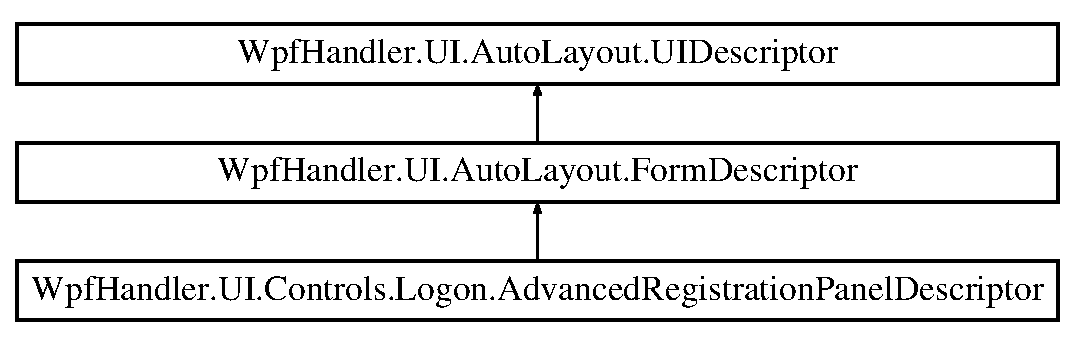
\includegraphics[height=3.000000cm]{dd/d32/class_wpf_handler_1_1_u_i_1_1_controls_1_1_logon_1_1_advanced_registration_panel_descriptor}
\end{center}
\end{figure}
\subsection*{Properties}
\begin{DoxyCompactItemize}
\item 
string \mbox{\hyperlink{class_wpf_handler_1_1_u_i_1_1_controls_1_1_logon_1_1_advanced_registration_panel_descriptor_ae8a21fc8856329480880595b0942afe7}{Email}} = \char`\"{}\char`\"{}\hspace{0.3cm}{\ttfamily  \mbox{[}get, set\mbox{]}}
\begin{DoxyCompactList}\small\item\em An user email. \end{DoxyCompactList}\item 
string \mbox{\hyperlink{class_wpf_handler_1_1_u_i_1_1_controls_1_1_logon_1_1_advanced_registration_panel_descriptor_a025efd3270fd44b0a8aafa7aa01fb50b}{Contact\+Phone}} = \char`\"{}\char`\"{}\hspace{0.3cm}{\ttfamily  \mbox{[}get, set\mbox{]}}
\begin{DoxyCompactList}\small\item\em An user cell. \end{DoxyCompactList}\item 
string \mbox{\hyperlink{class_wpf_handler_1_1_u_i_1_1_controls_1_1_logon_1_1_advanced_registration_panel_descriptor_a4fd87d8eab706d490c23ce21cbac3507}{Country}} = \char`\"{}\char`\"{}\hspace{0.3cm}{\ttfamily  \mbox{[}get, set\mbox{]}}
\begin{DoxyCompactList}\small\item\em A country where have been living a user. \end{DoxyCompactList}\item 
string \mbox{\hyperlink{class_wpf_handler_1_1_u_i_1_1_controls_1_1_logon_1_1_advanced_registration_panel_descriptor_a5918a7c8d33623d3cf9bc0bba7c295a2}{City}} = \char`\"{}\char`\"{}\hspace{0.3cm}{\ttfamily  \mbox{[}get, set\mbox{]}}
\begin{DoxyCompactList}\small\item\em A city where have been living a user. \end{DoxyCompactList}\item 
int \mbox{\hyperlink{class_wpf_handler_1_1_u_i_1_1_controls_1_1_logon_1_1_advanced_registration_panel_descriptor_a22e104a6aa8557c53ac8ab6bd53a3a0b}{Birth\+Year}} = 1960\hspace{0.3cm}{\ttfamily  \mbox{[}get, set\mbox{]}}
\begin{DoxyCompactList}\small\item\em A year of a user birth. \end{DoxyCompactList}\item 
int \mbox{\hyperlink{class_wpf_handler_1_1_u_i_1_1_controls_1_1_logon_1_1_advanced_registration_panel_descriptor_a54f4881fa4b6fbfd0aa8baa93993523c}{Birth\+Month}} = 1\hspace{0.3cm}{\ttfamily  \mbox{[}get, set\mbox{]}}
\begin{DoxyCompactList}\small\item\em A month of a user birth. \end{DoxyCompactList}\item 
int \mbox{\hyperlink{class_wpf_handler_1_1_u_i_1_1_controls_1_1_logon_1_1_advanced_registration_panel_descriptor_a30229eda915ba6cfdf9747e369f6afbe}{Birth\+Day}} = 1\hspace{0.3cm}{\ttfamily  \mbox{[}get, set\mbox{]}}
\begin{DoxyCompactList}\small\item\em A day of a user birth. \end{DoxyCompactList}\end{DoxyCompactItemize}
\subsection*{Additional Inherited Members}


\subsection{Detailed Description}
A form for storing advanced user\textquotesingle{}s info. 



\subsection{Property Documentation}
\mbox{\Hypertarget{class_wpf_handler_1_1_u_i_1_1_controls_1_1_logon_1_1_advanced_registration_panel_descriptor_a30229eda915ba6cfdf9747e369f6afbe}\label{class_wpf_handler_1_1_u_i_1_1_controls_1_1_logon_1_1_advanced_registration_panel_descriptor_a30229eda915ba6cfdf9747e369f6afbe}} 
\index{Wpf\+Handler\+::\+U\+I\+::\+Controls\+::\+Logon\+::\+Advanced\+Registration\+Panel\+Descriptor@{Wpf\+Handler\+::\+U\+I\+::\+Controls\+::\+Logon\+::\+Advanced\+Registration\+Panel\+Descriptor}!Birth\+Day@{Birth\+Day}}
\index{Birth\+Day@{Birth\+Day}!Wpf\+Handler\+::\+U\+I\+::\+Controls\+::\+Logon\+::\+Advanced\+Registration\+Panel\+Descriptor@{Wpf\+Handler\+::\+U\+I\+::\+Controls\+::\+Logon\+::\+Advanced\+Registration\+Panel\+Descriptor}}
\subsubsection{\texorpdfstring{Birth\+Day}{BirthDay}}
{\footnotesize\ttfamily int Wpf\+Handler.\+U\+I.\+Controls.\+Logon.\+Advanced\+Registration\+Panel\+Descriptor.\+Birth\+Day = 1\hspace{0.3cm}{\ttfamily [get]}, {\ttfamily [set]}}



A day of a user birth. 

\mbox{\Hypertarget{class_wpf_handler_1_1_u_i_1_1_controls_1_1_logon_1_1_advanced_registration_panel_descriptor_a54f4881fa4b6fbfd0aa8baa93993523c}\label{class_wpf_handler_1_1_u_i_1_1_controls_1_1_logon_1_1_advanced_registration_panel_descriptor_a54f4881fa4b6fbfd0aa8baa93993523c}} 
\index{Wpf\+Handler\+::\+U\+I\+::\+Controls\+::\+Logon\+::\+Advanced\+Registration\+Panel\+Descriptor@{Wpf\+Handler\+::\+U\+I\+::\+Controls\+::\+Logon\+::\+Advanced\+Registration\+Panel\+Descriptor}!Birth\+Month@{Birth\+Month}}
\index{Birth\+Month@{Birth\+Month}!Wpf\+Handler\+::\+U\+I\+::\+Controls\+::\+Logon\+::\+Advanced\+Registration\+Panel\+Descriptor@{Wpf\+Handler\+::\+U\+I\+::\+Controls\+::\+Logon\+::\+Advanced\+Registration\+Panel\+Descriptor}}
\subsubsection{\texorpdfstring{Birth\+Month}{BirthMonth}}
{\footnotesize\ttfamily int Wpf\+Handler.\+U\+I.\+Controls.\+Logon.\+Advanced\+Registration\+Panel\+Descriptor.\+Birth\+Month = 1\hspace{0.3cm}{\ttfamily [get]}, {\ttfamily [set]}}



A month of a user birth. 

\mbox{\Hypertarget{class_wpf_handler_1_1_u_i_1_1_controls_1_1_logon_1_1_advanced_registration_panel_descriptor_a22e104a6aa8557c53ac8ab6bd53a3a0b}\label{class_wpf_handler_1_1_u_i_1_1_controls_1_1_logon_1_1_advanced_registration_panel_descriptor_a22e104a6aa8557c53ac8ab6bd53a3a0b}} 
\index{Wpf\+Handler\+::\+U\+I\+::\+Controls\+::\+Logon\+::\+Advanced\+Registration\+Panel\+Descriptor@{Wpf\+Handler\+::\+U\+I\+::\+Controls\+::\+Logon\+::\+Advanced\+Registration\+Panel\+Descriptor}!Birth\+Year@{Birth\+Year}}
\index{Birth\+Year@{Birth\+Year}!Wpf\+Handler\+::\+U\+I\+::\+Controls\+::\+Logon\+::\+Advanced\+Registration\+Panel\+Descriptor@{Wpf\+Handler\+::\+U\+I\+::\+Controls\+::\+Logon\+::\+Advanced\+Registration\+Panel\+Descriptor}}
\subsubsection{\texorpdfstring{Birth\+Year}{BirthYear}}
{\footnotesize\ttfamily int Wpf\+Handler.\+U\+I.\+Controls.\+Logon.\+Advanced\+Registration\+Panel\+Descriptor.\+Birth\+Year = 1960\hspace{0.3cm}{\ttfamily [get]}, {\ttfamily [set]}}



A year of a user birth. 

\mbox{\Hypertarget{class_wpf_handler_1_1_u_i_1_1_controls_1_1_logon_1_1_advanced_registration_panel_descriptor_a5918a7c8d33623d3cf9bc0bba7c295a2}\label{class_wpf_handler_1_1_u_i_1_1_controls_1_1_logon_1_1_advanced_registration_panel_descriptor_a5918a7c8d33623d3cf9bc0bba7c295a2}} 
\index{Wpf\+Handler\+::\+U\+I\+::\+Controls\+::\+Logon\+::\+Advanced\+Registration\+Panel\+Descriptor@{Wpf\+Handler\+::\+U\+I\+::\+Controls\+::\+Logon\+::\+Advanced\+Registration\+Panel\+Descriptor}!City@{City}}
\index{City@{City}!Wpf\+Handler\+::\+U\+I\+::\+Controls\+::\+Logon\+::\+Advanced\+Registration\+Panel\+Descriptor@{Wpf\+Handler\+::\+U\+I\+::\+Controls\+::\+Logon\+::\+Advanced\+Registration\+Panel\+Descriptor}}
\subsubsection{\texorpdfstring{City}{City}}
{\footnotesize\ttfamily string Wpf\+Handler.\+U\+I.\+Controls.\+Logon.\+Advanced\+Registration\+Panel\+Descriptor.\+City = \char`\"{}\char`\"{}\hspace{0.3cm}{\ttfamily [get]}, {\ttfamily [set]}}



A city where have been living a user. 

\mbox{\Hypertarget{class_wpf_handler_1_1_u_i_1_1_controls_1_1_logon_1_1_advanced_registration_panel_descriptor_a025efd3270fd44b0a8aafa7aa01fb50b}\label{class_wpf_handler_1_1_u_i_1_1_controls_1_1_logon_1_1_advanced_registration_panel_descriptor_a025efd3270fd44b0a8aafa7aa01fb50b}} 
\index{Wpf\+Handler\+::\+U\+I\+::\+Controls\+::\+Logon\+::\+Advanced\+Registration\+Panel\+Descriptor@{Wpf\+Handler\+::\+U\+I\+::\+Controls\+::\+Logon\+::\+Advanced\+Registration\+Panel\+Descriptor}!Contact\+Phone@{Contact\+Phone}}
\index{Contact\+Phone@{Contact\+Phone}!Wpf\+Handler\+::\+U\+I\+::\+Controls\+::\+Logon\+::\+Advanced\+Registration\+Panel\+Descriptor@{Wpf\+Handler\+::\+U\+I\+::\+Controls\+::\+Logon\+::\+Advanced\+Registration\+Panel\+Descriptor}}
\subsubsection{\texorpdfstring{Contact\+Phone}{ContactPhone}}
{\footnotesize\ttfamily string Wpf\+Handler.\+U\+I.\+Controls.\+Logon.\+Advanced\+Registration\+Panel\+Descriptor.\+Contact\+Phone = \char`\"{}\char`\"{}\hspace{0.3cm}{\ttfamily [get]}, {\ttfamily [set]}}



An user cell. 

\mbox{\Hypertarget{class_wpf_handler_1_1_u_i_1_1_controls_1_1_logon_1_1_advanced_registration_panel_descriptor_a4fd87d8eab706d490c23ce21cbac3507}\label{class_wpf_handler_1_1_u_i_1_1_controls_1_1_logon_1_1_advanced_registration_panel_descriptor_a4fd87d8eab706d490c23ce21cbac3507}} 
\index{Wpf\+Handler\+::\+U\+I\+::\+Controls\+::\+Logon\+::\+Advanced\+Registration\+Panel\+Descriptor@{Wpf\+Handler\+::\+U\+I\+::\+Controls\+::\+Logon\+::\+Advanced\+Registration\+Panel\+Descriptor}!Country@{Country}}
\index{Country@{Country}!Wpf\+Handler\+::\+U\+I\+::\+Controls\+::\+Logon\+::\+Advanced\+Registration\+Panel\+Descriptor@{Wpf\+Handler\+::\+U\+I\+::\+Controls\+::\+Logon\+::\+Advanced\+Registration\+Panel\+Descriptor}}
\subsubsection{\texorpdfstring{Country}{Country}}
{\footnotesize\ttfamily string Wpf\+Handler.\+U\+I.\+Controls.\+Logon.\+Advanced\+Registration\+Panel\+Descriptor.\+Country = \char`\"{}\char`\"{}\hspace{0.3cm}{\ttfamily [get]}, {\ttfamily [set]}}



A country where have been living a user. 

\mbox{\Hypertarget{class_wpf_handler_1_1_u_i_1_1_controls_1_1_logon_1_1_advanced_registration_panel_descriptor_ae8a21fc8856329480880595b0942afe7}\label{class_wpf_handler_1_1_u_i_1_1_controls_1_1_logon_1_1_advanced_registration_panel_descriptor_ae8a21fc8856329480880595b0942afe7}} 
\index{Wpf\+Handler\+::\+U\+I\+::\+Controls\+::\+Logon\+::\+Advanced\+Registration\+Panel\+Descriptor@{Wpf\+Handler\+::\+U\+I\+::\+Controls\+::\+Logon\+::\+Advanced\+Registration\+Panel\+Descriptor}!Email@{Email}}
\index{Email@{Email}!Wpf\+Handler\+::\+U\+I\+::\+Controls\+::\+Logon\+::\+Advanced\+Registration\+Panel\+Descriptor@{Wpf\+Handler\+::\+U\+I\+::\+Controls\+::\+Logon\+::\+Advanced\+Registration\+Panel\+Descriptor}}
\subsubsection{\texorpdfstring{Email}{Email}}
{\footnotesize\ttfamily string Wpf\+Handler.\+U\+I.\+Controls.\+Logon.\+Advanced\+Registration\+Panel\+Descriptor.\+Email = \char`\"{}\char`\"{}\hspace{0.3cm}{\ttfamily [get]}, {\ttfamily [set]}}



An user email. 



The documentation for this class was generated from the following file\+:\begin{DoxyCompactItemize}
\item 
D\+:/\+Work/\+Git\+Hub/wpf-\/handler/\+Wpf\+Handler/\+U\+I/\+Controls/\+Logon/Advanced\+Registration\+Panel\+Descriptor.\+cs\end{DoxyCompactItemize}

\hypertarget{class_wpf_handler_1_1_dictionaries_1_1_a_p_i}{}\section{Wpf\+Handler.\+Dictionaries.\+A\+PI Class Reference}
\label{class_wpf_handler_1_1_dictionaries_1_1_a_p_i}\index{Wpf\+Handler.\+Dictionaries.\+A\+PI@{Wpf\+Handler.\+Dictionaries.\+A\+PI}}


Class that provide methods for controll W\+PF application localization.  


\subsection*{Static Public Member Functions}
\begin{DoxyCompactItemize}
\item 
static void \mbox{\hyperlink{class_wpf_handler_1_1_dictionaries_1_1_a_p_i_ac9aafbe351f06f0c20de39508d3e8852}{Load\+X\+A\+M\+L\+\_\+\+Thems}} (string theme\+Code)
\begin{DoxyCompactList}\small\item\em Scaning for language dictionaries in X\+A\+ML files, and load them to Merged dictionaries. Loading new theme by code if found. Leave already loaded if overrided dictionary not found. \end{DoxyCompactList}\item 
static void \mbox{\hyperlink{class_wpf_handler_1_1_dictionaries_1_1_a_p_i_a0de06b29ec542383dbdc470bb9a7c98e}{Update\+Dictionaries\+Group}} (string directory, string group\+Code, params string\mbox{[}$\,$\mbox{]} sub\+Codes)
\begin{DoxyCompactList}\small\item\em Updating dictionaries loaded for certain group. \end{DoxyCompactList}\item 
static void \mbox{\hyperlink{class_wpf_handler_1_1_dictionaries_1_1_a_p_i_a2611ee5407fe0a4cde1a2490a54d759e}{Clear\+Dictionaries\+Group}} (string group\+Code)
\begin{DoxyCompactList}\small\item\em Clearing all loaded dictionaries from certain group. \end{DoxyCompactList}\end{DoxyCompactItemize}


\subsection{Detailed Description}
Class that provide methods for controll W\+PF application localization. 



\subsection{Member Function Documentation}
\mbox{\Hypertarget{class_wpf_handler_1_1_dictionaries_1_1_a_p_i_a2611ee5407fe0a4cde1a2490a54d759e}\label{class_wpf_handler_1_1_dictionaries_1_1_a_p_i_a2611ee5407fe0a4cde1a2490a54d759e}} 
\index{Wpf\+Handler\+::\+Dictionaries\+::\+A\+PI@{Wpf\+Handler\+::\+Dictionaries\+::\+A\+PI}!Clear\+Dictionaries\+Group@{Clear\+Dictionaries\+Group}}
\index{Clear\+Dictionaries\+Group@{Clear\+Dictionaries\+Group}!Wpf\+Handler\+::\+Dictionaries\+::\+A\+PI@{Wpf\+Handler\+::\+Dictionaries\+::\+A\+PI}}
\subsubsection{\texorpdfstring{Clear\+Dictionaries\+Group()}{ClearDictionariesGroup()}}
{\footnotesize\ttfamily static void Wpf\+Handler.\+Dictionaries.\+A\+P\+I.\+Clear\+Dictionaries\+Group (\begin{DoxyParamCaption}\item[{string}]{group\+Code }\end{DoxyParamCaption})\hspace{0.3cm}{\ttfamily [static]}}



Clearing all loaded dictionaries from certain group. 


\begin{DoxyParams}{Parameters}
{\em group\+Code} & The unique code of the dictioaries group. Allows to determite the diferend purposes of the plugins like localization (lang), \mbox{\hyperlink{namespace_wpf_handler_1_1_u_i}{UI}} themes (theme), etc.\\
\hline
\end{DoxyParams}
\mbox{\Hypertarget{class_wpf_handler_1_1_dictionaries_1_1_a_p_i_ac9aafbe351f06f0c20de39508d3e8852}\label{class_wpf_handler_1_1_dictionaries_1_1_a_p_i_ac9aafbe351f06f0c20de39508d3e8852}} 
\index{Wpf\+Handler\+::\+Dictionaries\+::\+A\+PI@{Wpf\+Handler\+::\+Dictionaries\+::\+A\+PI}!Load\+X\+A\+M\+L\+\_\+\+Thems@{Load\+X\+A\+M\+L\+\_\+\+Thems}}
\index{Load\+X\+A\+M\+L\+\_\+\+Thems@{Load\+X\+A\+M\+L\+\_\+\+Thems}!Wpf\+Handler\+::\+Dictionaries\+::\+A\+PI@{Wpf\+Handler\+::\+Dictionaries\+::\+A\+PI}}
\subsubsection{\texorpdfstring{Load\+X\+A\+M\+L\+\_\+\+Thems()}{LoadXAML\_Thems()}}
{\footnotesize\ttfamily static void Wpf\+Handler.\+Dictionaries.\+A\+P\+I.\+Load\+X\+A\+M\+L\+\_\+\+Thems (\begin{DoxyParamCaption}\item[{string}]{theme\+Code }\end{DoxyParamCaption})\hspace{0.3cm}{\ttfamily [static]}}



Scaning for language dictionaries in X\+A\+ML files, and load them to Merged dictionaries. Loading new theme by code if found. Leave already loaded if overrided dictionary not found. 

Require files format\+: $\ast$.theme.\+T\+H\+E\+M\+E\+\_\+\+C\+O\+D\+E.\+xaml, where theme code equal current theme selected on the app. Example\+: plugin.\+feed.\+theme.\+blue\+Theme.\+xaml 


\begin{DoxyParams}{Parameters}
{\em theme\+Code} & \\
\hline
\end{DoxyParams}
\mbox{\Hypertarget{class_wpf_handler_1_1_dictionaries_1_1_a_p_i_a0de06b29ec542383dbdc470bb9a7c98e}\label{class_wpf_handler_1_1_dictionaries_1_1_a_p_i_a0de06b29ec542383dbdc470bb9a7c98e}} 
\index{Wpf\+Handler\+::\+Dictionaries\+::\+A\+PI@{Wpf\+Handler\+::\+Dictionaries\+::\+A\+PI}!Update\+Dictionaries\+Group@{Update\+Dictionaries\+Group}}
\index{Update\+Dictionaries\+Group@{Update\+Dictionaries\+Group}!Wpf\+Handler\+::\+Dictionaries\+::\+A\+PI@{Wpf\+Handler\+::\+Dictionaries\+::\+A\+PI}}
\subsubsection{\texorpdfstring{Update\+Dictionaries\+Group()}{UpdateDictionariesGroup()}}
{\footnotesize\ttfamily static void Wpf\+Handler.\+Dictionaries.\+A\+P\+I.\+Update\+Dictionaries\+Group (\begin{DoxyParamCaption}\item[{string}]{directory,  }\item[{string}]{group\+Code,  }\item[{params string \mbox{[}$\,$\mbox{]}}]{sub\+Codes }\end{DoxyParamCaption})\hspace{0.3cm}{\ttfamily [static]}}



Updating dictionaries loaded for certain group. 


\begin{DoxyParams}{Parameters}
{\em directory} & The directory where stored dicrionaties. Using Search\+Option.\+All\+Directories suring search. \\
\hline
{\em group\+Code} & The unique code of the dictioaries group. Allows to determite the diferend purposes of the plugins like localization (lang), \mbox{\hyperlink{namespace_wpf_handler_1_1_u_i}{UI}} themes (theme), etc.\\
\hline
{\em sub\+Codes} & Codes that will be required from group of plugins. Will be looced in order of prefernces. Lower index -\/ more prefered. Will load any exist in case if any requested code not found.\\
\hline
\end{DoxyParams}
Exmples\+: Culture code for localization plugins. Theme code for design plugins. 

The documentation for this class was generated from the following file\+:\begin{DoxyCompactItemize}
\item 
D\+:/\+Work/\+Git\+Hub/wpf-\/handler/\+Wpf\+Handler/\+Dictionaries/A\+P\+I.\+cs\end{DoxyCompactItemize}

\hypertarget{class_wpf_handler_1_1_plugins_1_1_a_p_i}{}\section{Wpf\+Handler.\+Plugins.\+A\+PI Class Reference}
\label{class_wpf_handler_1_1_plugins_1_1_a_p_i}\index{Wpf\+Handler.\+Plugins.\+A\+PI@{Wpf\+Handler.\+Plugins.\+A\+PI}}


Class that profide simplifyed way to integrate W\+PF plugins to client.  


\subsection*{Static Public Member Functions}
\begin{DoxyCompactItemize}
\item 
static I\+Enumerable$<$ \mbox{\hyperlink{interface_wpf_handler_1_1_plugins_1_1_i_plugin}{I\+Plugin}} $>$ \mbox{\hyperlink{class_wpf_handler_1_1_plugins_1_1_a_p_i_ae2d2c46617f63533ddc20f08166b6c6e}{Load\+Plugins\+Enumerable}} ()
\begin{DoxyCompactList}\small\item\em Load plugins from assembly and instiniate them to list. \end{DoxyCompactList}\item 
static System.\+Collections.\+Object\+Model.\+Observable\+Collection$<$ \mbox{\hyperlink{interface_wpf_handler_1_1_plugins_1_1_i_plugin}{I\+Plugin}} $>$ \mbox{\hyperlink{class_wpf_handler_1_1_plugins_1_1_a_p_i_aa797a592049cf57860ee422586fcccac}{Load\+Plugins\+Collection}} ()
\begin{DoxyCompactList}\small\item\em Load plugins from assembly and instiniate them to list. \end{DoxyCompactList}\item 
static void \mbox{\hyperlink{class_wpf_handler_1_1_plugins_1_1_a_p_i_a4dbfd1cc62cfb8def6f17d8c622e0fd8}{Open\+G\+UI}} (\mbox{\hyperlink{interface_wpf_handler_1_1_plugins_1_1_i_plugin}{I\+Plugin}} plugin, string panel\+Name=\char`\"{}canvas\char`\"{})
\begin{DoxyCompactList}\small\item\em Oppenig plugin G\+UI. \end{DoxyCompactList}\item 
static void \mbox{\hyperlink{class_wpf_handler_1_1_plugins_1_1_a_p_i_aaa094e4b6d27c336e8f0f76acc04ba20}{Sort\+By\+Domains}} (I\+Collection$<$ \mbox{\hyperlink{interface_wpf_handler_1_1_plugins_1_1_i_plugin}{I\+Plugin}} $>$ plugins)
\begin{DoxyCompactList}\small\item\em Sorting items in collection by tomain recommended orders and hierarchy depth. \end{DoxyCompactList}\end{DoxyCompactItemize}


\subsection{Detailed Description}
Class that profide simplifyed way to integrate W\+PF plugins to client. 



\subsection{Member Function Documentation}
\mbox{\Hypertarget{class_wpf_handler_1_1_plugins_1_1_a_p_i_aa797a592049cf57860ee422586fcccac}\label{class_wpf_handler_1_1_plugins_1_1_a_p_i_aa797a592049cf57860ee422586fcccac}} 
\index{Wpf\+Handler\+::\+Plugins\+::\+A\+PI@{Wpf\+Handler\+::\+Plugins\+::\+A\+PI}!Load\+Plugins\+Collection@{Load\+Plugins\+Collection}}
\index{Load\+Plugins\+Collection@{Load\+Plugins\+Collection}!Wpf\+Handler\+::\+Plugins\+::\+A\+PI@{Wpf\+Handler\+::\+Plugins\+::\+A\+PI}}
\subsubsection{\texorpdfstring{Load\+Plugins\+Collection()}{LoadPluginsCollection()}}
{\footnotesize\ttfamily static System.\+Collections.\+Object\+Model.\+Observable\+Collection$<$\mbox{\hyperlink{interface_wpf_handler_1_1_plugins_1_1_i_plugin}{I\+Plugin}}$>$ Wpf\+Handler.\+Plugins.\+A\+P\+I.\+Load\+Plugins\+Collection (\begin{DoxyParamCaption}{ }\end{DoxyParamCaption})\hspace{0.3cm}{\ttfamily [static]}}



Load plugins from assembly and instiniate them to list. 

\mbox{\Hypertarget{class_wpf_handler_1_1_plugins_1_1_a_p_i_ae2d2c46617f63533ddc20f08166b6c6e}\label{class_wpf_handler_1_1_plugins_1_1_a_p_i_ae2d2c46617f63533ddc20f08166b6c6e}} 
\index{Wpf\+Handler\+::\+Plugins\+::\+A\+PI@{Wpf\+Handler\+::\+Plugins\+::\+A\+PI}!Load\+Plugins\+Enumerable@{Load\+Plugins\+Enumerable}}
\index{Load\+Plugins\+Enumerable@{Load\+Plugins\+Enumerable}!Wpf\+Handler\+::\+Plugins\+::\+A\+PI@{Wpf\+Handler\+::\+Plugins\+::\+A\+PI}}
\subsubsection{\texorpdfstring{Load\+Plugins\+Enumerable()}{LoadPluginsEnumerable()}}
{\footnotesize\ttfamily static I\+Enumerable$<$\mbox{\hyperlink{interface_wpf_handler_1_1_plugins_1_1_i_plugin}{I\+Plugin}}$>$ Wpf\+Handler.\+Plugins.\+A\+P\+I.\+Load\+Plugins\+Enumerable (\begin{DoxyParamCaption}{ }\end{DoxyParamCaption})\hspace{0.3cm}{\ttfamily [static]}}



Load plugins from assembly and instiniate them to list. 

\begin{DoxyReturn}{Returns}

\end{DoxyReturn}
\mbox{\Hypertarget{class_wpf_handler_1_1_plugins_1_1_a_p_i_a4dbfd1cc62cfb8def6f17d8c622e0fd8}\label{class_wpf_handler_1_1_plugins_1_1_a_p_i_a4dbfd1cc62cfb8def6f17d8c622e0fd8}} 
\index{Wpf\+Handler\+::\+Plugins\+::\+A\+PI@{Wpf\+Handler\+::\+Plugins\+::\+A\+PI}!Open\+G\+UI@{Open\+G\+UI}}
\index{Open\+G\+UI@{Open\+G\+UI}!Wpf\+Handler\+::\+Plugins\+::\+A\+PI@{Wpf\+Handler\+::\+Plugins\+::\+A\+PI}}
\subsubsection{\texorpdfstring{Open\+G\+U\+I()}{OpenGUI()}}
{\footnotesize\ttfamily static void Wpf\+Handler.\+Plugins.\+A\+P\+I.\+Open\+G\+UI (\begin{DoxyParamCaption}\item[{\mbox{\hyperlink{interface_wpf_handler_1_1_plugins_1_1_i_plugin}{I\+Plugin}}}]{plugin,  }\item[{string}]{panel\+Name = {\ttfamily \char`\"{}canvas\char`\"{}} }\end{DoxyParamCaption})\hspace{0.3cm}{\ttfamily [static]}}



Oppenig plugin G\+UI. 


\begin{DoxyParams}{Parameters}
{\em plugin} & Target plugin.\\
\hline
{\em panel\+Name} & Name of the Panel control that would contrin content.\\
\hline
\end{DoxyParams}
\mbox{\Hypertarget{class_wpf_handler_1_1_plugins_1_1_a_p_i_aaa094e4b6d27c336e8f0f76acc04ba20}\label{class_wpf_handler_1_1_plugins_1_1_a_p_i_aaa094e4b6d27c336e8f0f76acc04ba20}} 
\index{Wpf\+Handler\+::\+Plugins\+::\+A\+PI@{Wpf\+Handler\+::\+Plugins\+::\+A\+PI}!Sort\+By\+Domains@{Sort\+By\+Domains}}
\index{Sort\+By\+Domains@{Sort\+By\+Domains}!Wpf\+Handler\+::\+Plugins\+::\+A\+PI@{Wpf\+Handler\+::\+Plugins\+::\+A\+PI}}
\subsubsection{\texorpdfstring{Sort\+By\+Domains()}{SortByDomains()}}
{\footnotesize\ttfamily static void Wpf\+Handler.\+Plugins.\+A\+P\+I.\+Sort\+By\+Domains (\begin{DoxyParamCaption}\item[{I\+Collection$<$ \mbox{\hyperlink{interface_wpf_handler_1_1_plugins_1_1_i_plugin}{I\+Plugin}} $>$}]{plugins }\end{DoxyParamCaption})\hspace{0.3cm}{\ttfamily [static]}}



Sorting items in collection by tomain recommended orders and hierarchy depth. 


\begin{DoxyParams}{Parameters}
{\em plugins} & \\
\hline
\end{DoxyParams}


The documentation for this class was generated from the following file\+:\begin{DoxyCompactItemize}
\item 
D\+:/\+Work/\+Git\+Hub/wpf-\/handler/\+Wpf\+Handler/\+Plugins/A\+P\+I.\+cs\end{DoxyCompactItemize}

\hypertarget{class_wpf_handler_1_1_u_i_1_1_controls_1_1_auto_collection}{}\section{Wpf\+Handler.\+U\+I.\+Controls.\+Auto\+Collection Class Reference}
\label{class_wpf_handler_1_1_u_i_1_1_controls_1_1_auto_collection}\index{Wpf\+Handler.\+U\+I.\+Controls.\+Auto\+Collection@{Wpf\+Handler.\+U\+I.\+Controls.\+Auto\+Collection}}


\mbox{\hyperlink{class_wpf_handler_1_1_u_i_1_1_controls_1_1_auto_collection}{Auto\+Collection}}  


Inheritance diagram for Wpf\+Handler.\+U\+I.\+Controls.\+Auto\+Collection\+:\begin{figure}[H]
\begin{center}
\leavevmode
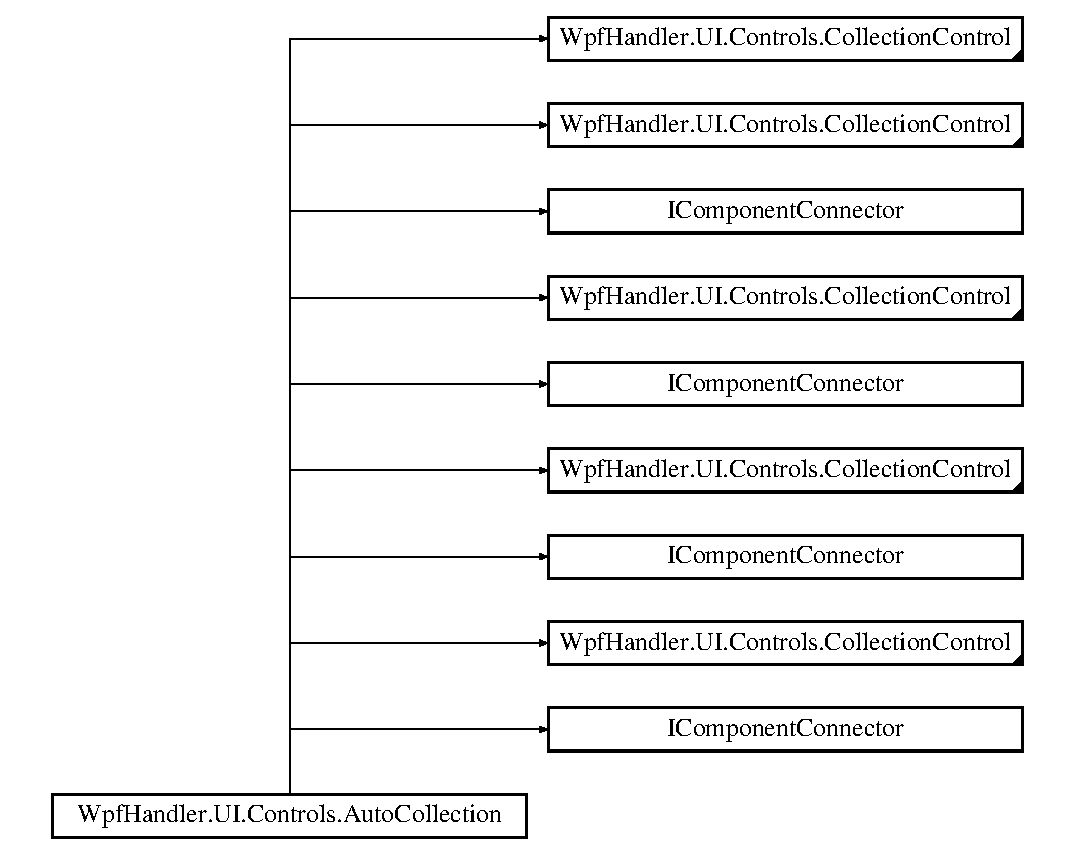
\includegraphics[height=10.000000cm]{d2/d28/class_wpf_handler_1_1_u_i_1_1_controls_1_1_auto_collection}
\end{center}
\end{figure}
\subsection*{Public Member Functions}
\begin{DoxyCompactItemize}
\item 
void \mbox{\hyperlink{class_wpf_handler_1_1_u_i_1_1_controls_1_1_auto_collection_a625f859b619ad02bc4943b8086a95dfd}{Initialize\+Component}} ()
\begin{DoxyCompactList}\small\item\em Initialize\+Component \end{DoxyCompactList}\item 
void \mbox{\hyperlink{class_wpf_handler_1_1_u_i_1_1_controls_1_1_auto_collection_a625f859b619ad02bc4943b8086a95dfd}{Initialize\+Component}} ()
\begin{DoxyCompactList}\small\item\em Initialize\+Component \end{DoxyCompactList}\item 
void \mbox{\hyperlink{class_wpf_handler_1_1_u_i_1_1_controls_1_1_auto_collection_a625f859b619ad02bc4943b8086a95dfd}{Initialize\+Component}} ()
\begin{DoxyCompactList}\small\item\em Initialize\+Component \end{DoxyCompactList}\item 
void \mbox{\hyperlink{class_wpf_handler_1_1_u_i_1_1_controls_1_1_auto_collection_a625f859b619ad02bc4943b8086a95dfd}{Initialize\+Component}} ()
\begin{DoxyCompactList}\small\item\em Initialize\+Component \end{DoxyCompactList}\item 
\mbox{\hyperlink{class_wpf_handler_1_1_u_i_1_1_controls_1_1_auto_collection_a8bc71a7c43dfeca1d6ff113b12088c28}{Auto\+Collection}} ()
\begin{DoxyCompactList}\small\item\em Initialize that component. Looking for the {\ttfamily \mbox{\hyperlink{class_wpf_handler_1_1_u_i_1_1_controls_1_1_auto_collection}{Auto\+Collection}}} Style resource. Use default if not found. \end{DoxyCompactList}\end{DoxyCompactItemize}
\subsection*{Public Attributes}
\begin{DoxyCompactItemize}
\item 
override List\+Box \mbox{\hyperlink{class_wpf_handler_1_1_u_i_1_1_controls_1_1_auto_collection_a144774a121d36e2207fd0e39dd67a074}{List\+Content}} =$>$ content\+Panel
\begin{DoxyCompactList}\small\item\em Bindted lsit element that will manage items. \end{DoxyCompactList}\item 
Action$<$ object $>$ \mbox{\hyperlink{class_wpf_handler_1_1_u_i_1_1_controls_1_1_auto_collection_a996c2d451bb6e072a9ff03ce6a21b5fc}{On\+Add\+Click}}
\begin{DoxyCompactList}\small\item\em The delegate that will be called during Add button click. In case if initialized then will be called instead default. \end{DoxyCompactList}\item 
Action$<$ object $>$ \mbox{\hyperlink{class_wpf_handler_1_1_u_i_1_1_controls_1_1_auto_collection_a6130a353d0fadfaaf9bc17881406354f}{On\+Remove\+Click}}
\begin{DoxyCompactList}\small\item\em The delegate that will be called during Remove button click. In case if initialized then will be called instead default. \end{DoxyCompactList}\end{DoxyCompactItemize}
\subsection*{Static Public Attributes}
\begin{DoxyCompactItemize}
\item 
static readonly Dependency\+Property \mbox{\hyperlink{class_wpf_handler_1_1_u_i_1_1_controls_1_1_auto_collection_ad8966a126d82307e2796bba38737518e}{Backplate\+Background\+Property}}
\begin{DoxyCompactList}\small\item\em Property that bridging control\textquotesingle{}s property between X\+A\+ML and code. \end{DoxyCompactList}\item 
static readonly Dependency\+Property \mbox{\hyperlink{class_wpf_handler_1_1_u_i_1_1_controls_1_1_auto_collection_a0d827839ba40e106ecbe9470a7e4c53b}{Spliter\+Color\+Property}}
\begin{DoxyCompactList}\small\item\em Property that bridging control\textquotesingle{}s property between X\+A\+ML and code. \end{DoxyCompactList}\item 
static readonly Dependency\+Property \mbox{\hyperlink{class_wpf_handler_1_1_u_i_1_1_controls_1_1_auto_collection_a7f269c1eaefddc9f23e9aa7c523740de}{Corner\+Radius\+Property}}
\begin{DoxyCompactList}\small\item\em Property that bridging control\textquotesingle{}s property between X\+A\+ML and code. \end{DoxyCompactList}\item 
static readonly Dependency\+Property \mbox{\hyperlink{class_wpf_handler_1_1_u_i_1_1_controls_1_1_auto_collection_a142911c55327f71205f61bf4f32f2e35}{Spliters\+Draw\+Property}}
\begin{DoxyCompactList}\small\item\em Property that bridging control\textquotesingle{}s property between X\+A\+ML and code. \end{DoxyCompactList}\item 
static readonly Dependency\+Property \mbox{\hyperlink{class_wpf_handler_1_1_u_i_1_1_controls_1_1_auto_collection_aff46124c0cd77747b466fa231ce4f264}{Add\+Button\+Visibile\+Property}}
\begin{DoxyCompactList}\small\item\em Property that bridging control\textquotesingle{}s property between X\+A\+ML and code. \end{DoxyCompactList}\item 
static readonly Dependency\+Property \mbox{\hyperlink{class_wpf_handler_1_1_u_i_1_1_controls_1_1_auto_collection_a85a427be17693babbaa5943c04c2ca2d}{Remove\+Button\+Visibile\+Property}}
\begin{DoxyCompactList}\small\item\em Property that bridging control\textquotesingle{}s property between X\+A\+ML and code. \end{DoxyCompactList}\item 
static readonly Routed\+Event \mbox{\hyperlink{class_wpf_handler_1_1_u_i_1_1_controls_1_1_auto_collection_adb3a377a24d9b0fefc0d58cf0c8e6289}{On\+Add\+Event}}
\begin{DoxyCompactList}\small\item\em Property that bridging control\textquotesingle{}s property between X\+A\+ML and code. \end{DoxyCompactList}\item 
static readonly Routed\+Event \mbox{\hyperlink{class_wpf_handler_1_1_u_i_1_1_controls_1_1_auto_collection_a55213a701b1defa4c6a490d25f083fe4}{On\+Remove\+Event}}
\begin{DoxyCompactList}\small\item\em Property that bridging control\textquotesingle{}s property between X\+A\+ML and code. \end{DoxyCompactList}\end{DoxyCompactItemize}
\subsection*{Protected Member Functions}
\begin{DoxyCompactItemize}
\item 
void \mbox{\hyperlink{class_wpf_handler_1_1_u_i_1_1_controls_1_1_auto_collection_a01ab069c42e1737cebb4bb813ec8aa06}{Recompute\+Layout}} ()
\begin{DoxyCompactList}\small\item\em Recomputing element layout. \end{DoxyCompactList}\item 
override Framework\+Element \mbox{\hyperlink{class_wpf_handler_1_1_u_i_1_1_controls_1_1_auto_collection_a7cea6362ca2a31dca7bca6ab1f39142d}{Item\+Registration}} (int index)
\begin{DoxyCompactList}\small\item\em Registrating an item of the list. \end{DoxyCompactList}\item 
void \mbox{\hyperlink{class_wpf_handler_1_1_u_i_1_1_controls_1_1_auto_collection_ac229b39e23e0d2d9895f4897d1116e70}{On\+Add}} (object sender)
\begin{DoxyCompactList}\small\item\em Occurs when user pressing add button. Adding an element of the type that described in the first generic type argument of the source I\+List. \end{DoxyCompactList}\item 
void \mbox{\hyperlink{class_wpf_handler_1_1_u_i_1_1_controls_1_1_auto_collection_addd4df92578229539c28bc4db8121d68}{On\+Remove}} (object sender)
\begin{DoxyCompactList}\small\item\em Occurs when user pressing remove button. \end{DoxyCompactList}\end{DoxyCompactItemize}
\subsection*{Package Functions}
\begin{DoxyCompactItemize}
\item 
\mbox{\Hypertarget{class_wpf_handler_1_1_u_i_1_1_controls_1_1_auto_collection_a99c959811ba90ac28a922c4fca6354c5}\label{class_wpf_handler_1_1_u_i_1_1_controls_1_1_auto_collection_a99c959811ba90ac28a922c4fca6354c5}} 
System.\+Delegate {\bfseries \+\_\+\+Create\+Delegate} (System.\+Type delegate\+Type, string handler)
\item 
\mbox{\Hypertarget{class_wpf_handler_1_1_u_i_1_1_controls_1_1_auto_collection_a99c959811ba90ac28a922c4fca6354c5}\label{class_wpf_handler_1_1_u_i_1_1_controls_1_1_auto_collection_a99c959811ba90ac28a922c4fca6354c5}} 
System.\+Delegate {\bfseries \+\_\+\+Create\+Delegate} (System.\+Type delegate\+Type, string handler)
\item 
\mbox{\Hypertarget{class_wpf_handler_1_1_u_i_1_1_controls_1_1_auto_collection_a99c959811ba90ac28a922c4fca6354c5}\label{class_wpf_handler_1_1_u_i_1_1_controls_1_1_auto_collection_a99c959811ba90ac28a922c4fca6354c5}} 
System.\+Delegate {\bfseries \+\_\+\+Create\+Delegate} (System.\+Type delegate\+Type, string handler)
\item 
\mbox{\Hypertarget{class_wpf_handler_1_1_u_i_1_1_controls_1_1_auto_collection_a99c959811ba90ac28a922c4fca6354c5}\label{class_wpf_handler_1_1_u_i_1_1_controls_1_1_auto_collection_a99c959811ba90ac28a922c4fca6354c5}} 
System.\+Delegate {\bfseries \+\_\+\+Create\+Delegate} (System.\+Type delegate\+Type, string handler)
\end{DoxyCompactItemize}
\subsection*{Package Attributes}
\begin{DoxyCompactItemize}
\item 
\mbox{\Hypertarget{class_wpf_handler_1_1_u_i_1_1_controls_1_1_auto_collection_a7dc53e4e449c84aaf0224e67178c75ee}\label{class_wpf_handler_1_1_u_i_1_1_controls_1_1_auto_collection_a7dc53e4e449c84aaf0224e67178c75ee}} 
System.\+Windows.\+Shapes.\+Rectangle {\bfseries buttons\+Bridge}
\item 
\mbox{\Hypertarget{class_wpf_handler_1_1_u_i_1_1_controls_1_1_auto_collection_a7789a472b03e85cbe2549c9013be00bf}\label{class_wpf_handler_1_1_u_i_1_1_controls_1_1_auto_collection_a7789a472b03e85cbe2549c9013be00bf}} 
System.\+Windows.\+Controls.\+Grid {\bfseries add\+Button\+Group}
\item 
\mbox{\Hypertarget{class_wpf_handler_1_1_u_i_1_1_controls_1_1_auto_collection_a13695c847269d9dbe772f19a851fe3e2}\label{class_wpf_handler_1_1_u_i_1_1_controls_1_1_auto_collection_a13695c847269d9dbe772f19a851fe3e2}} 
System.\+Windows.\+Controls.\+Grid {\bfseries remove\+Button\+Group}
\item 
\mbox{\Hypertarget{class_wpf_handler_1_1_u_i_1_1_controls_1_1_auto_collection_a63c727fa284523170ce868104ff84fdd}\label{class_wpf_handler_1_1_u_i_1_1_controls_1_1_auto_collection_a63c727fa284523170ce868104ff84fdd}} 
System.\+Windows.\+Shapes.\+Rectangle {\bfseries corner\+Backplate}
\item 
\mbox{\Hypertarget{class_wpf_handler_1_1_u_i_1_1_controls_1_1_auto_collection_a9ac5ea400a66d488ed009aaf7ed690f3}\label{class_wpf_handler_1_1_u_i_1_1_controls_1_1_auto_collection_a9ac5ea400a66d488ed009aaf7ed690f3}} 
System.\+Windows.\+Controls.\+Grid {\bfseries collection\+Panel}
\item 
\mbox{\Hypertarget{class_wpf_handler_1_1_u_i_1_1_controls_1_1_auto_collection_a02f27ec31a3f8119adb18c4d7985d8df}\label{class_wpf_handler_1_1_u_i_1_1_controls_1_1_auto_collection_a02f27ec31a3f8119adb18c4d7985d8df}} 
System.\+Windows.\+Controls.\+Scroll\+Viewer {\bfseries veiw}
\item 
\mbox{\Hypertarget{class_wpf_handler_1_1_u_i_1_1_controls_1_1_auto_collection_a8c09e909985500e234de87514b262f6c}\label{class_wpf_handler_1_1_u_i_1_1_controls_1_1_auto_collection_a8c09e909985500e234de87514b262f6c}} 
System.\+Windows.\+Controls.\+List\+Box {\bfseries content\+Panel}
\end{DoxyCompactItemize}
\subsection*{Properties}
\begin{DoxyCompactItemize}
\item 
bool \mbox{\hyperlink{class_wpf_handler_1_1_u_i_1_1_controls_1_1_auto_collection_a5b53cdaeabbf4958eb0391475f060771}{Add\+Button\+Visibile}}\hspace{0.3cm}{\ttfamily  \mbox{[}get, set\mbox{]}}
\begin{DoxyCompactList}\small\item\em If the add button available for an user. \end{DoxyCompactList}\item 
bool \mbox{\hyperlink{class_wpf_handler_1_1_u_i_1_1_controls_1_1_auto_collection_af64aaec7162358b87294c5b7f77c8e54}{Remove\+Button\+Visibile}}\hspace{0.3cm}{\ttfamily  \mbox{[}get, set\mbox{]}}
\begin{DoxyCompactList}\small\item\em Is the remove button available for an user. \end{DoxyCompactList}\item 
bool \mbox{\hyperlink{class_wpf_handler_1_1_u_i_1_1_controls_1_1_auto_collection_a78b75144a4f57f1ec4d6027388afbd5d}{Spliters\+Draw}} = true\hspace{0.3cm}{\ttfamily  \mbox{[}get, set\mbox{]}}
\begin{DoxyCompactList}\small\item\em Is the spliting lines between content elements are visible. \end{DoxyCompactList}\item 
double \mbox{\hyperlink{class_wpf_handler_1_1_u_i_1_1_controls_1_1_auto_collection_a0a78d9c621857e9a61e19cba5001589d}{Corner\+Radius}}\hspace{0.3cm}{\ttfamily  \mbox{[}get, set\mbox{]}}
\begin{DoxyCompactList}\small\item\em Radius of the rounded corders. \end{DoxyCompactList}\item 
Brush \mbox{\hyperlink{class_wpf_handler_1_1_u_i_1_1_controls_1_1_auto_collection_a9234690dcc653145332286c86afa4904}{Spliter\+Color}}\hspace{0.3cm}{\ttfamily  \mbox{[}get, set\mbox{]}}
\begin{DoxyCompactList}\small\item\em Color of the spliters. \end{DoxyCompactList}\item 
Brush \mbox{\hyperlink{class_wpf_handler_1_1_u_i_1_1_controls_1_1_auto_collection_af74226c7fb905acd0a3040ba4b677713}{Backplate\+Background}}\hspace{0.3cm}{\ttfamily  \mbox{[}get, set\mbox{]}}
\begin{DoxyCompactList}\small\item\em Color of the backplate. \end{DoxyCompactList}\end{DoxyCompactItemize}
\subsection*{Private Member Functions}
\begin{DoxyCompactItemize}
\item 
\mbox{\Hypertarget{class_wpf_handler_1_1_u_i_1_1_controls_1_1_auto_collection_ae27a9f5902ca092611b2dfcae06aac84}\label{class_wpf_handler_1_1_u_i_1_1_controls_1_1_auto_collection_ae27a9f5902ca092611b2dfcae06aac84}} 
void System.\+Windows.\+Markup.\+I\+Component\+Connector. {\bfseries Connect} (int connection\+Id, object target)
\item 
\mbox{\Hypertarget{class_wpf_handler_1_1_u_i_1_1_controls_1_1_auto_collection_ae27a9f5902ca092611b2dfcae06aac84}\label{class_wpf_handler_1_1_u_i_1_1_controls_1_1_auto_collection_ae27a9f5902ca092611b2dfcae06aac84}} 
void System.\+Windows.\+Markup.\+I\+Component\+Connector. {\bfseries Connect} (int connection\+Id, object target)
\item 
\mbox{\Hypertarget{class_wpf_handler_1_1_u_i_1_1_controls_1_1_auto_collection_ae27a9f5902ca092611b2dfcae06aac84}\label{class_wpf_handler_1_1_u_i_1_1_controls_1_1_auto_collection_ae27a9f5902ca092611b2dfcae06aac84}} 
void System.\+Windows.\+Markup.\+I\+Component\+Connector. {\bfseries Connect} (int connection\+Id, object target)
\item 
\mbox{\Hypertarget{class_wpf_handler_1_1_u_i_1_1_controls_1_1_auto_collection_ae27a9f5902ca092611b2dfcae06aac84}\label{class_wpf_handler_1_1_u_i_1_1_controls_1_1_auto_collection_ae27a9f5902ca092611b2dfcae06aac84}} 
void System.\+Windows.\+Markup.\+I\+Component\+Connector. {\bfseries Connect} (int connection\+Id, object target)
\item 
void \mbox{\hyperlink{class_wpf_handler_1_1_u_i_1_1_controls_1_1_auto_collection_a1a849b598ba5dadbb9466b3b758377cf}{Auto\+Collection\+\_\+\+Loaded}} (object sender, Routed\+Event\+Args e)
\begin{DoxyCompactList}\small\item\em Occurs when the contol is loaded. \end{DoxyCompactList}\end{DoxyCompactItemize}
\subsection*{Private Attributes}
\begin{DoxyCompactItemize}
\item 
\mbox{\Hypertarget{class_wpf_handler_1_1_u_i_1_1_controls_1_1_auto_collection_a9b1198e458151ced3611a7f6062506e9}\label{class_wpf_handler_1_1_u_i_1_1_controls_1_1_auto_collection_a9b1198e458151ced3611a7f6062506e9}} 
bool {\bfseries \+\_\+content\+Loaded}
\end{DoxyCompactItemize}
\subsection*{Additional Inherited Members}


\subsection{Detailed Description}
\mbox{\hyperlink{class_wpf_handler_1_1_u_i_1_1_controls_1_1_auto_collection}{Auto\+Collection}} 

Creating \mbox{\hyperlink{namespace_wpf_handler_1_1_u_i}{UI}} element for work with binded collections. 

\subsection{Constructor \& Destructor Documentation}
\mbox{\Hypertarget{class_wpf_handler_1_1_u_i_1_1_controls_1_1_auto_collection_a8bc71a7c43dfeca1d6ff113b12088c28}\label{class_wpf_handler_1_1_u_i_1_1_controls_1_1_auto_collection_a8bc71a7c43dfeca1d6ff113b12088c28}} 
\index{Wpf\+Handler\+::\+U\+I\+::\+Controls\+::\+Auto\+Collection@{Wpf\+Handler\+::\+U\+I\+::\+Controls\+::\+Auto\+Collection}!Auto\+Collection@{Auto\+Collection}}
\index{Auto\+Collection@{Auto\+Collection}!Wpf\+Handler\+::\+U\+I\+::\+Controls\+::\+Auto\+Collection@{Wpf\+Handler\+::\+U\+I\+::\+Controls\+::\+Auto\+Collection}}
\subsubsection{\texorpdfstring{Auto\+Collection()}{AutoCollection()}}
{\footnotesize\ttfamily Wpf\+Handler.\+U\+I.\+Controls.\+Auto\+Collection.\+Auto\+Collection (\begin{DoxyParamCaption}{ }\end{DoxyParamCaption})}



Initialize that component. Looking for the {\ttfamily \mbox{\hyperlink{class_wpf_handler_1_1_u_i_1_1_controls_1_1_auto_collection}{Auto\+Collection}}} Style resource. Use default if not found. 



\subsection{Member Function Documentation}
\mbox{\Hypertarget{class_wpf_handler_1_1_u_i_1_1_controls_1_1_auto_collection_a1a849b598ba5dadbb9466b3b758377cf}\label{class_wpf_handler_1_1_u_i_1_1_controls_1_1_auto_collection_a1a849b598ba5dadbb9466b3b758377cf}} 
\index{Wpf\+Handler\+::\+U\+I\+::\+Controls\+::\+Auto\+Collection@{Wpf\+Handler\+::\+U\+I\+::\+Controls\+::\+Auto\+Collection}!Auto\+Collection\+\_\+\+Loaded@{Auto\+Collection\+\_\+\+Loaded}}
\index{Auto\+Collection\+\_\+\+Loaded@{Auto\+Collection\+\_\+\+Loaded}!Wpf\+Handler\+::\+U\+I\+::\+Controls\+::\+Auto\+Collection@{Wpf\+Handler\+::\+U\+I\+::\+Controls\+::\+Auto\+Collection}}
\subsubsection{\texorpdfstring{Auto\+Collection\+\_\+\+Loaded()}{AutoCollection\_Loaded()}}
{\footnotesize\ttfamily void Wpf\+Handler.\+U\+I.\+Controls.\+Auto\+Collection.\+Auto\+Collection\+\_\+\+Loaded (\begin{DoxyParamCaption}\item[{object}]{sender,  }\item[{Routed\+Event\+Args}]{e }\end{DoxyParamCaption})\hspace{0.3cm}{\ttfamily [private]}}



Occurs when the contol is loaded. 


\begin{DoxyParams}{Parameters}
{\em sender} & \\
\hline
{\em e} & \\
\hline
\end{DoxyParams}
\mbox{\Hypertarget{class_wpf_handler_1_1_u_i_1_1_controls_1_1_auto_collection_a625f859b619ad02bc4943b8086a95dfd}\label{class_wpf_handler_1_1_u_i_1_1_controls_1_1_auto_collection_a625f859b619ad02bc4943b8086a95dfd}} 
\index{Wpf\+Handler\+::\+U\+I\+::\+Controls\+::\+Auto\+Collection@{Wpf\+Handler\+::\+U\+I\+::\+Controls\+::\+Auto\+Collection}!Initialize\+Component@{Initialize\+Component}}
\index{Initialize\+Component@{Initialize\+Component}!Wpf\+Handler\+::\+U\+I\+::\+Controls\+::\+Auto\+Collection@{Wpf\+Handler\+::\+U\+I\+::\+Controls\+::\+Auto\+Collection}}
\subsubsection{\texorpdfstring{Initialize\+Component()}{InitializeComponent()}\hspace{0.1cm}{\footnotesize\ttfamily [1/4]}}
{\footnotesize\ttfamily void Wpf\+Handler.\+U\+I.\+Controls.\+Auto\+Collection.\+Initialize\+Component (\begin{DoxyParamCaption}{ }\end{DoxyParamCaption})}



Initialize\+Component 

\mbox{\Hypertarget{class_wpf_handler_1_1_u_i_1_1_controls_1_1_auto_collection_a625f859b619ad02bc4943b8086a95dfd}\label{class_wpf_handler_1_1_u_i_1_1_controls_1_1_auto_collection_a625f859b619ad02bc4943b8086a95dfd}} 
\index{Wpf\+Handler\+::\+U\+I\+::\+Controls\+::\+Auto\+Collection@{Wpf\+Handler\+::\+U\+I\+::\+Controls\+::\+Auto\+Collection}!Initialize\+Component@{Initialize\+Component}}
\index{Initialize\+Component@{Initialize\+Component}!Wpf\+Handler\+::\+U\+I\+::\+Controls\+::\+Auto\+Collection@{Wpf\+Handler\+::\+U\+I\+::\+Controls\+::\+Auto\+Collection}}
\subsubsection{\texorpdfstring{Initialize\+Component()}{InitializeComponent()}\hspace{0.1cm}{\footnotesize\ttfamily [2/4]}}
{\footnotesize\ttfamily void Wpf\+Handler.\+U\+I.\+Controls.\+Auto\+Collection.\+Initialize\+Component (\begin{DoxyParamCaption}{ }\end{DoxyParamCaption})}



Initialize\+Component 

\mbox{\Hypertarget{class_wpf_handler_1_1_u_i_1_1_controls_1_1_auto_collection_a625f859b619ad02bc4943b8086a95dfd}\label{class_wpf_handler_1_1_u_i_1_1_controls_1_1_auto_collection_a625f859b619ad02bc4943b8086a95dfd}} 
\index{Wpf\+Handler\+::\+U\+I\+::\+Controls\+::\+Auto\+Collection@{Wpf\+Handler\+::\+U\+I\+::\+Controls\+::\+Auto\+Collection}!Initialize\+Component@{Initialize\+Component}}
\index{Initialize\+Component@{Initialize\+Component}!Wpf\+Handler\+::\+U\+I\+::\+Controls\+::\+Auto\+Collection@{Wpf\+Handler\+::\+U\+I\+::\+Controls\+::\+Auto\+Collection}}
\subsubsection{\texorpdfstring{Initialize\+Component()}{InitializeComponent()}\hspace{0.1cm}{\footnotesize\ttfamily [3/4]}}
{\footnotesize\ttfamily void Wpf\+Handler.\+U\+I.\+Controls.\+Auto\+Collection.\+Initialize\+Component (\begin{DoxyParamCaption}{ }\end{DoxyParamCaption})}



Initialize\+Component 

\mbox{\Hypertarget{class_wpf_handler_1_1_u_i_1_1_controls_1_1_auto_collection_a625f859b619ad02bc4943b8086a95dfd}\label{class_wpf_handler_1_1_u_i_1_1_controls_1_1_auto_collection_a625f859b619ad02bc4943b8086a95dfd}} 
\index{Wpf\+Handler\+::\+U\+I\+::\+Controls\+::\+Auto\+Collection@{Wpf\+Handler\+::\+U\+I\+::\+Controls\+::\+Auto\+Collection}!Initialize\+Component@{Initialize\+Component}}
\index{Initialize\+Component@{Initialize\+Component}!Wpf\+Handler\+::\+U\+I\+::\+Controls\+::\+Auto\+Collection@{Wpf\+Handler\+::\+U\+I\+::\+Controls\+::\+Auto\+Collection}}
\subsubsection{\texorpdfstring{Initialize\+Component()}{InitializeComponent()}\hspace{0.1cm}{\footnotesize\ttfamily [4/4]}}
{\footnotesize\ttfamily void Wpf\+Handler.\+U\+I.\+Controls.\+Auto\+Collection.\+Initialize\+Component (\begin{DoxyParamCaption}{ }\end{DoxyParamCaption})}



Initialize\+Component 

\mbox{\Hypertarget{class_wpf_handler_1_1_u_i_1_1_controls_1_1_auto_collection_a7cea6362ca2a31dca7bca6ab1f39142d}\label{class_wpf_handler_1_1_u_i_1_1_controls_1_1_auto_collection_a7cea6362ca2a31dca7bca6ab1f39142d}} 
\index{Wpf\+Handler\+::\+U\+I\+::\+Controls\+::\+Auto\+Collection@{Wpf\+Handler\+::\+U\+I\+::\+Controls\+::\+Auto\+Collection}!Item\+Registration@{Item\+Registration}}
\index{Item\+Registration@{Item\+Registration}!Wpf\+Handler\+::\+U\+I\+::\+Controls\+::\+Auto\+Collection@{Wpf\+Handler\+::\+U\+I\+::\+Controls\+::\+Auto\+Collection}}
\subsubsection{\texorpdfstring{Item\+Registration()}{ItemRegistration()}}
{\footnotesize\ttfamily override Framework\+Element Wpf\+Handler.\+U\+I.\+Controls.\+Auto\+Collection.\+Item\+Registration (\begin{DoxyParamCaption}\item[{int}]{index }\end{DoxyParamCaption})\hspace{0.3cm}{\ttfamily [protected]}, {\ttfamily [virtual]}}



Registrating an item of the list. 


\begin{DoxyParams}{Parameters}
{\em index} & An index of item into the source collection.\\
\hline
\end{DoxyParams}
\begin{DoxyReturn}{Returns}

\end{DoxyReturn}


Reimplemented from \mbox{\hyperlink{class_wpf_handler_1_1_u_i_1_1_controls_1_1_collection_control_af375cbcb4d351b4d104b2706d39b8303}{Wpf\+Handler.\+U\+I.\+Controls.\+Collection\+Control}}.

\mbox{\Hypertarget{class_wpf_handler_1_1_u_i_1_1_controls_1_1_auto_collection_ac229b39e23e0d2d9895f4897d1116e70}\label{class_wpf_handler_1_1_u_i_1_1_controls_1_1_auto_collection_ac229b39e23e0d2d9895f4897d1116e70}} 
\index{Wpf\+Handler\+::\+U\+I\+::\+Controls\+::\+Auto\+Collection@{Wpf\+Handler\+::\+U\+I\+::\+Controls\+::\+Auto\+Collection}!On\+Add@{On\+Add}}
\index{On\+Add@{On\+Add}!Wpf\+Handler\+::\+U\+I\+::\+Controls\+::\+Auto\+Collection@{Wpf\+Handler\+::\+U\+I\+::\+Controls\+::\+Auto\+Collection}}
\subsubsection{\texorpdfstring{On\+Add()}{OnAdd()}}
{\footnotesize\ttfamily void Wpf\+Handler.\+U\+I.\+Controls.\+Auto\+Collection.\+On\+Add (\begin{DoxyParamCaption}\item[{object}]{sender }\end{DoxyParamCaption})\hspace{0.3cm}{\ttfamily [protected]}}



Occurs when user pressing add button. Adding an element of the type that described in the first generic type argument of the source I\+List. 


\begin{DoxyParams}{Parameters}
{\em sender} & An element that caused that callback.\\
\hline
\end{DoxyParams}
\mbox{\Hypertarget{class_wpf_handler_1_1_u_i_1_1_controls_1_1_auto_collection_addd4df92578229539c28bc4db8121d68}\label{class_wpf_handler_1_1_u_i_1_1_controls_1_1_auto_collection_addd4df92578229539c28bc4db8121d68}} 
\index{Wpf\+Handler\+::\+U\+I\+::\+Controls\+::\+Auto\+Collection@{Wpf\+Handler\+::\+U\+I\+::\+Controls\+::\+Auto\+Collection}!On\+Remove@{On\+Remove}}
\index{On\+Remove@{On\+Remove}!Wpf\+Handler\+::\+U\+I\+::\+Controls\+::\+Auto\+Collection@{Wpf\+Handler\+::\+U\+I\+::\+Controls\+::\+Auto\+Collection}}
\subsubsection{\texorpdfstring{On\+Remove()}{OnRemove()}}
{\footnotesize\ttfamily void Wpf\+Handler.\+U\+I.\+Controls.\+Auto\+Collection.\+On\+Remove (\begin{DoxyParamCaption}\item[{object}]{sender }\end{DoxyParamCaption})\hspace{0.3cm}{\ttfamily [protected]}}



Occurs when user pressing remove button. 


\begin{DoxyParams}{Parameters}
{\em sender} & $>$An element that caused that callback.\\
\hline
\end{DoxyParams}
\mbox{\Hypertarget{class_wpf_handler_1_1_u_i_1_1_controls_1_1_auto_collection_a01ab069c42e1737cebb4bb813ec8aa06}\label{class_wpf_handler_1_1_u_i_1_1_controls_1_1_auto_collection_a01ab069c42e1737cebb4bb813ec8aa06}} 
\index{Wpf\+Handler\+::\+U\+I\+::\+Controls\+::\+Auto\+Collection@{Wpf\+Handler\+::\+U\+I\+::\+Controls\+::\+Auto\+Collection}!Recompute\+Layout@{Recompute\+Layout}}
\index{Recompute\+Layout@{Recompute\+Layout}!Wpf\+Handler\+::\+U\+I\+::\+Controls\+::\+Auto\+Collection@{Wpf\+Handler\+::\+U\+I\+::\+Controls\+::\+Auto\+Collection}}
\subsubsection{\texorpdfstring{Recompute\+Layout()}{RecomputeLayout()}}
{\footnotesize\ttfamily void Wpf\+Handler.\+U\+I.\+Controls.\+Auto\+Collection.\+Recompute\+Layout (\begin{DoxyParamCaption}{ }\end{DoxyParamCaption})\hspace{0.3cm}{\ttfamily [protected]}}



Recomputing element layout. 



\subsection{Member Data Documentation}
\mbox{\Hypertarget{class_wpf_handler_1_1_u_i_1_1_controls_1_1_auto_collection_aff46124c0cd77747b466fa231ce4f264}\label{class_wpf_handler_1_1_u_i_1_1_controls_1_1_auto_collection_aff46124c0cd77747b466fa231ce4f264}} 
\index{Wpf\+Handler\+::\+U\+I\+::\+Controls\+::\+Auto\+Collection@{Wpf\+Handler\+::\+U\+I\+::\+Controls\+::\+Auto\+Collection}!Add\+Button\+Visibile\+Property@{Add\+Button\+Visibile\+Property}}
\index{Add\+Button\+Visibile\+Property@{Add\+Button\+Visibile\+Property}!Wpf\+Handler\+::\+U\+I\+::\+Controls\+::\+Auto\+Collection@{Wpf\+Handler\+::\+U\+I\+::\+Controls\+::\+Auto\+Collection}}
\subsubsection{\texorpdfstring{Add\+Button\+Visibile\+Property}{AddButtonVisibileProperty}}
{\footnotesize\ttfamily readonly Dependency\+Property Wpf\+Handler.\+U\+I.\+Controls.\+Auto\+Collection.\+Add\+Button\+Visibile\+Property\hspace{0.3cm}{\ttfamily [static]}}

{\bfseries Initial value\+:}
\begin{DoxyCode}
= DependencyProperty.Register(
          \textcolor{stringliteral}{"AddButtonVisibile"}, typeof(\textcolor{keywordtype}{bool}), typeof(\mbox{\hyperlink{class_wpf_handler_1_1_u_i_1_1_controls_1_1_auto_collection_a8bc71a7c43dfeca1d6ff113b12088c28}{AutoCollection}}),
          \textcolor{keyword}{new} PropertyMetadata(\textcolor{keyword}{true}))
\end{DoxyCode}


Property that bridging control\textquotesingle{}s property between X\+A\+ML and code. 

\mbox{\Hypertarget{class_wpf_handler_1_1_u_i_1_1_controls_1_1_auto_collection_ad8966a126d82307e2796bba38737518e}\label{class_wpf_handler_1_1_u_i_1_1_controls_1_1_auto_collection_ad8966a126d82307e2796bba38737518e}} 
\index{Wpf\+Handler\+::\+U\+I\+::\+Controls\+::\+Auto\+Collection@{Wpf\+Handler\+::\+U\+I\+::\+Controls\+::\+Auto\+Collection}!Backplate\+Background\+Property@{Backplate\+Background\+Property}}
\index{Backplate\+Background\+Property@{Backplate\+Background\+Property}!Wpf\+Handler\+::\+U\+I\+::\+Controls\+::\+Auto\+Collection@{Wpf\+Handler\+::\+U\+I\+::\+Controls\+::\+Auto\+Collection}}
\subsubsection{\texorpdfstring{Backplate\+Background\+Property}{BackplateBackgroundProperty}}
{\footnotesize\ttfamily readonly Dependency\+Property Wpf\+Handler.\+U\+I.\+Controls.\+Auto\+Collection.\+Backplate\+Background\+Property\hspace{0.3cm}{\ttfamily [static]}}

{\bfseries Initial value\+:}
\begin{DoxyCode}
= DependencyProperty.Register(
          \textcolor{stringliteral}{"BackplateBackground"}, typeof(Brush), typeof(\mbox{\hyperlink{class_wpf_handler_1_1_u_i_1_1_controls_1_1_auto_collection_a8bc71a7c43dfeca1d6ff113b12088c28}{AutoCollection}}),
          \textcolor{keyword}{new} PropertyMetadata(Brushes.WhiteSmoke))
\end{DoxyCode}


Property that bridging control\textquotesingle{}s property between X\+A\+ML and code. 

\mbox{\Hypertarget{class_wpf_handler_1_1_u_i_1_1_controls_1_1_auto_collection_a7f269c1eaefddc9f23e9aa7c523740de}\label{class_wpf_handler_1_1_u_i_1_1_controls_1_1_auto_collection_a7f269c1eaefddc9f23e9aa7c523740de}} 
\index{Wpf\+Handler\+::\+U\+I\+::\+Controls\+::\+Auto\+Collection@{Wpf\+Handler\+::\+U\+I\+::\+Controls\+::\+Auto\+Collection}!Corner\+Radius\+Property@{Corner\+Radius\+Property}}
\index{Corner\+Radius\+Property@{Corner\+Radius\+Property}!Wpf\+Handler\+::\+U\+I\+::\+Controls\+::\+Auto\+Collection@{Wpf\+Handler\+::\+U\+I\+::\+Controls\+::\+Auto\+Collection}}
\subsubsection{\texorpdfstring{Corner\+Radius\+Property}{CornerRadiusProperty}}
{\footnotesize\ttfamily readonly Dependency\+Property Wpf\+Handler.\+U\+I.\+Controls.\+Auto\+Collection.\+Corner\+Radius\+Property\hspace{0.3cm}{\ttfamily [static]}}

{\bfseries Initial value\+:}
\begin{DoxyCode}
= DependencyProperty.Register(
          \textcolor{stringliteral}{"CornerRadius"}, typeof(\textcolor{keywordtype}{double}), typeof(\mbox{\hyperlink{class_wpf_handler_1_1_u_i_1_1_controls_1_1_auto_collection_a8bc71a7c43dfeca1d6ff113b12088c28}{AutoCollection}}),
          \textcolor{keyword}{new} PropertyMetadata(7.0d))
\end{DoxyCode}


Property that bridging control\textquotesingle{}s property between X\+A\+ML and code. 

\mbox{\Hypertarget{class_wpf_handler_1_1_u_i_1_1_controls_1_1_auto_collection_a144774a121d36e2207fd0e39dd67a074}\label{class_wpf_handler_1_1_u_i_1_1_controls_1_1_auto_collection_a144774a121d36e2207fd0e39dd67a074}} 
\index{Wpf\+Handler\+::\+U\+I\+::\+Controls\+::\+Auto\+Collection@{Wpf\+Handler\+::\+U\+I\+::\+Controls\+::\+Auto\+Collection}!List\+Content@{List\+Content}}
\index{List\+Content@{List\+Content}!Wpf\+Handler\+::\+U\+I\+::\+Controls\+::\+Auto\+Collection@{Wpf\+Handler\+::\+U\+I\+::\+Controls\+::\+Auto\+Collection}}
\subsubsection{\texorpdfstring{List\+Content}{ListContent}}
{\footnotesize\ttfamily override List\+Box Wpf\+Handler.\+U\+I.\+Controls.\+Auto\+Collection.\+List\+Content =$>$ content\+Panel}



Bindted lsit element that will manage items. 

\mbox{\Hypertarget{class_wpf_handler_1_1_u_i_1_1_controls_1_1_auto_collection_a996c2d451bb6e072a9ff03ce6a21b5fc}\label{class_wpf_handler_1_1_u_i_1_1_controls_1_1_auto_collection_a996c2d451bb6e072a9ff03ce6a21b5fc}} 
\index{Wpf\+Handler\+::\+U\+I\+::\+Controls\+::\+Auto\+Collection@{Wpf\+Handler\+::\+U\+I\+::\+Controls\+::\+Auto\+Collection}!On\+Add\+Click@{On\+Add\+Click}}
\index{On\+Add\+Click@{On\+Add\+Click}!Wpf\+Handler\+::\+U\+I\+::\+Controls\+::\+Auto\+Collection@{Wpf\+Handler\+::\+U\+I\+::\+Controls\+::\+Auto\+Collection}}
\subsubsection{\texorpdfstring{On\+Add\+Click}{OnAddClick}}
{\footnotesize\ttfamily Action$<$object$>$ Wpf\+Handler.\+U\+I.\+Controls.\+Auto\+Collection.\+On\+Add\+Click}



The delegate that will be called during Add button click. In case if initialized then will be called instead default. 

\mbox{\Hypertarget{class_wpf_handler_1_1_u_i_1_1_controls_1_1_auto_collection_adb3a377a24d9b0fefc0d58cf0c8e6289}\label{class_wpf_handler_1_1_u_i_1_1_controls_1_1_auto_collection_adb3a377a24d9b0fefc0d58cf0c8e6289}} 
\index{Wpf\+Handler\+::\+U\+I\+::\+Controls\+::\+Auto\+Collection@{Wpf\+Handler\+::\+U\+I\+::\+Controls\+::\+Auto\+Collection}!On\+Add\+Event@{On\+Add\+Event}}
\index{On\+Add\+Event@{On\+Add\+Event}!Wpf\+Handler\+::\+U\+I\+::\+Controls\+::\+Auto\+Collection@{Wpf\+Handler\+::\+U\+I\+::\+Controls\+::\+Auto\+Collection}}
\subsubsection{\texorpdfstring{On\+Add\+Event}{OnAddEvent}}
{\footnotesize\ttfamily readonly Routed\+Event Wpf\+Handler.\+U\+I.\+Controls.\+Auto\+Collection.\+On\+Add\+Event\hspace{0.3cm}{\ttfamily [static]}}

{\bfseries Initial value\+:}
\begin{DoxyCode}
= EventManager.RegisterRoutedEvent(\textcolor{stringliteral}{"OnAddClick"},
            RoutingStrategy.Bubble, typeof(RoutedEventHandler), typeof(
      \mbox{\hyperlink{class_wpf_handler_1_1_u_i_1_1_controls_1_1_auto_collection_a8bc71a7c43dfeca1d6ff113b12088c28}{AutoCollection}}))
\end{DoxyCode}


Property that bridging control\textquotesingle{}s property between X\+A\+ML and code. 

\mbox{\Hypertarget{class_wpf_handler_1_1_u_i_1_1_controls_1_1_auto_collection_a6130a353d0fadfaaf9bc17881406354f}\label{class_wpf_handler_1_1_u_i_1_1_controls_1_1_auto_collection_a6130a353d0fadfaaf9bc17881406354f}} 
\index{Wpf\+Handler\+::\+U\+I\+::\+Controls\+::\+Auto\+Collection@{Wpf\+Handler\+::\+U\+I\+::\+Controls\+::\+Auto\+Collection}!On\+Remove\+Click@{On\+Remove\+Click}}
\index{On\+Remove\+Click@{On\+Remove\+Click}!Wpf\+Handler\+::\+U\+I\+::\+Controls\+::\+Auto\+Collection@{Wpf\+Handler\+::\+U\+I\+::\+Controls\+::\+Auto\+Collection}}
\subsubsection{\texorpdfstring{On\+Remove\+Click}{OnRemoveClick}}
{\footnotesize\ttfamily Action$<$object$>$ Wpf\+Handler.\+U\+I.\+Controls.\+Auto\+Collection.\+On\+Remove\+Click}



The delegate that will be called during Remove button click. In case if initialized then will be called instead default. 

\mbox{\Hypertarget{class_wpf_handler_1_1_u_i_1_1_controls_1_1_auto_collection_a55213a701b1defa4c6a490d25f083fe4}\label{class_wpf_handler_1_1_u_i_1_1_controls_1_1_auto_collection_a55213a701b1defa4c6a490d25f083fe4}} 
\index{Wpf\+Handler\+::\+U\+I\+::\+Controls\+::\+Auto\+Collection@{Wpf\+Handler\+::\+U\+I\+::\+Controls\+::\+Auto\+Collection}!On\+Remove\+Event@{On\+Remove\+Event}}
\index{On\+Remove\+Event@{On\+Remove\+Event}!Wpf\+Handler\+::\+U\+I\+::\+Controls\+::\+Auto\+Collection@{Wpf\+Handler\+::\+U\+I\+::\+Controls\+::\+Auto\+Collection}}
\subsubsection{\texorpdfstring{On\+Remove\+Event}{OnRemoveEvent}}
{\footnotesize\ttfamily readonly Routed\+Event Wpf\+Handler.\+U\+I.\+Controls.\+Auto\+Collection.\+On\+Remove\+Event\hspace{0.3cm}{\ttfamily [static]}}

{\bfseries Initial value\+:}
\begin{DoxyCode}
= EventManager.RegisterRoutedEvent(\textcolor{stringliteral}{"OnRemoveClick"},
            RoutingStrategy.Bubble, typeof(RoutedEventHandler), typeof(
      \mbox{\hyperlink{class_wpf_handler_1_1_u_i_1_1_controls_1_1_auto_collection_a8bc71a7c43dfeca1d6ff113b12088c28}{AutoCollection}}))
\end{DoxyCode}


Property that bridging control\textquotesingle{}s property between X\+A\+ML and code. 

\mbox{\Hypertarget{class_wpf_handler_1_1_u_i_1_1_controls_1_1_auto_collection_a85a427be17693babbaa5943c04c2ca2d}\label{class_wpf_handler_1_1_u_i_1_1_controls_1_1_auto_collection_a85a427be17693babbaa5943c04c2ca2d}} 
\index{Wpf\+Handler\+::\+U\+I\+::\+Controls\+::\+Auto\+Collection@{Wpf\+Handler\+::\+U\+I\+::\+Controls\+::\+Auto\+Collection}!Remove\+Button\+Visibile\+Property@{Remove\+Button\+Visibile\+Property}}
\index{Remove\+Button\+Visibile\+Property@{Remove\+Button\+Visibile\+Property}!Wpf\+Handler\+::\+U\+I\+::\+Controls\+::\+Auto\+Collection@{Wpf\+Handler\+::\+U\+I\+::\+Controls\+::\+Auto\+Collection}}
\subsubsection{\texorpdfstring{Remove\+Button\+Visibile\+Property}{RemoveButtonVisibileProperty}}
{\footnotesize\ttfamily readonly Dependency\+Property Wpf\+Handler.\+U\+I.\+Controls.\+Auto\+Collection.\+Remove\+Button\+Visibile\+Property\hspace{0.3cm}{\ttfamily [static]}}

{\bfseries Initial value\+:}
\begin{DoxyCode}
= DependencyProperty.Register(
          \textcolor{stringliteral}{"RemoveButtonVisibile"}, typeof(\textcolor{keywordtype}{bool}), typeof(\mbox{\hyperlink{class_wpf_handler_1_1_u_i_1_1_controls_1_1_auto_collection_a8bc71a7c43dfeca1d6ff113b12088c28}{AutoCollection}}),
          \textcolor{keyword}{new} PropertyMetadata(\textcolor{keyword}{true}))
\end{DoxyCode}


Property that bridging control\textquotesingle{}s property between X\+A\+ML and code. 

\mbox{\Hypertarget{class_wpf_handler_1_1_u_i_1_1_controls_1_1_auto_collection_a0d827839ba40e106ecbe9470a7e4c53b}\label{class_wpf_handler_1_1_u_i_1_1_controls_1_1_auto_collection_a0d827839ba40e106ecbe9470a7e4c53b}} 
\index{Wpf\+Handler\+::\+U\+I\+::\+Controls\+::\+Auto\+Collection@{Wpf\+Handler\+::\+U\+I\+::\+Controls\+::\+Auto\+Collection}!Spliter\+Color\+Property@{Spliter\+Color\+Property}}
\index{Spliter\+Color\+Property@{Spliter\+Color\+Property}!Wpf\+Handler\+::\+U\+I\+::\+Controls\+::\+Auto\+Collection@{Wpf\+Handler\+::\+U\+I\+::\+Controls\+::\+Auto\+Collection}}
\subsubsection{\texorpdfstring{Spliter\+Color\+Property}{SpliterColorProperty}}
{\footnotesize\ttfamily readonly Dependency\+Property Wpf\+Handler.\+U\+I.\+Controls.\+Auto\+Collection.\+Spliter\+Color\+Property\hspace{0.3cm}{\ttfamily [static]}}

{\bfseries Initial value\+:}
\begin{DoxyCode}
= DependencyProperty.Register(
          \textcolor{stringliteral}{"SpliterColor"}, typeof(Brush), typeof(\mbox{\hyperlink{class_wpf_handler_1_1_u_i_1_1_controls_1_1_auto_collection_a8bc71a7c43dfeca1d6ff113b12088c28}{AutoCollection}}),
          \textcolor{keyword}{new} PropertyMetadata(Brushes.LightGray))
\end{DoxyCode}


Property that bridging control\textquotesingle{}s property between X\+A\+ML and code. 

\mbox{\Hypertarget{class_wpf_handler_1_1_u_i_1_1_controls_1_1_auto_collection_a142911c55327f71205f61bf4f32f2e35}\label{class_wpf_handler_1_1_u_i_1_1_controls_1_1_auto_collection_a142911c55327f71205f61bf4f32f2e35}} 
\index{Wpf\+Handler\+::\+U\+I\+::\+Controls\+::\+Auto\+Collection@{Wpf\+Handler\+::\+U\+I\+::\+Controls\+::\+Auto\+Collection}!Spliters\+Draw\+Property@{Spliters\+Draw\+Property}}
\index{Spliters\+Draw\+Property@{Spliters\+Draw\+Property}!Wpf\+Handler\+::\+U\+I\+::\+Controls\+::\+Auto\+Collection@{Wpf\+Handler\+::\+U\+I\+::\+Controls\+::\+Auto\+Collection}}
\subsubsection{\texorpdfstring{Spliters\+Draw\+Property}{SplitersDrawProperty}}
{\footnotesize\ttfamily readonly Dependency\+Property Wpf\+Handler.\+U\+I.\+Controls.\+Auto\+Collection.\+Spliters\+Draw\+Property\hspace{0.3cm}{\ttfamily [static]}}

{\bfseries Initial value\+:}
\begin{DoxyCode}
= DependencyProperty.Register(
          \textcolor{stringliteral}{"SplitersDraw"}, typeof(\textcolor{keywordtype}{bool}), typeof(\mbox{\hyperlink{class_wpf_handler_1_1_u_i_1_1_controls_1_1_auto_collection_a8bc71a7c43dfeca1d6ff113b12088c28}{AutoCollection}}),
          \textcolor{keyword}{new} PropertyMetadata(\textcolor{keyword}{true}))
\end{DoxyCode}


Property that bridging control\textquotesingle{}s property between X\+A\+ML and code. 



\subsection{Property Documentation}
\mbox{\Hypertarget{class_wpf_handler_1_1_u_i_1_1_controls_1_1_auto_collection_a5b53cdaeabbf4958eb0391475f060771}\label{class_wpf_handler_1_1_u_i_1_1_controls_1_1_auto_collection_a5b53cdaeabbf4958eb0391475f060771}} 
\index{Wpf\+Handler\+::\+U\+I\+::\+Controls\+::\+Auto\+Collection@{Wpf\+Handler\+::\+U\+I\+::\+Controls\+::\+Auto\+Collection}!Add\+Button\+Visibile@{Add\+Button\+Visibile}}
\index{Add\+Button\+Visibile@{Add\+Button\+Visibile}!Wpf\+Handler\+::\+U\+I\+::\+Controls\+::\+Auto\+Collection@{Wpf\+Handler\+::\+U\+I\+::\+Controls\+::\+Auto\+Collection}}
\subsubsection{\texorpdfstring{Add\+Button\+Visibile}{AddButtonVisibile}}
{\footnotesize\ttfamily bool Wpf\+Handler.\+U\+I.\+Controls.\+Auto\+Collection.\+Add\+Button\+Visibile\hspace{0.3cm}{\ttfamily [get]}, {\ttfamily [set]}}



If the add button available for an user. 

\mbox{\Hypertarget{class_wpf_handler_1_1_u_i_1_1_controls_1_1_auto_collection_af74226c7fb905acd0a3040ba4b677713}\label{class_wpf_handler_1_1_u_i_1_1_controls_1_1_auto_collection_af74226c7fb905acd0a3040ba4b677713}} 
\index{Wpf\+Handler\+::\+U\+I\+::\+Controls\+::\+Auto\+Collection@{Wpf\+Handler\+::\+U\+I\+::\+Controls\+::\+Auto\+Collection}!Backplate\+Background@{Backplate\+Background}}
\index{Backplate\+Background@{Backplate\+Background}!Wpf\+Handler\+::\+U\+I\+::\+Controls\+::\+Auto\+Collection@{Wpf\+Handler\+::\+U\+I\+::\+Controls\+::\+Auto\+Collection}}
\subsubsection{\texorpdfstring{Backplate\+Background}{BackplateBackground}}
{\footnotesize\ttfamily Brush Wpf\+Handler.\+U\+I.\+Controls.\+Auto\+Collection.\+Backplate\+Background\hspace{0.3cm}{\ttfamily [get]}, {\ttfamily [set]}}



Color of the backplate. 

\mbox{\Hypertarget{class_wpf_handler_1_1_u_i_1_1_controls_1_1_auto_collection_a0a78d9c621857e9a61e19cba5001589d}\label{class_wpf_handler_1_1_u_i_1_1_controls_1_1_auto_collection_a0a78d9c621857e9a61e19cba5001589d}} 
\index{Wpf\+Handler\+::\+U\+I\+::\+Controls\+::\+Auto\+Collection@{Wpf\+Handler\+::\+U\+I\+::\+Controls\+::\+Auto\+Collection}!Corner\+Radius@{Corner\+Radius}}
\index{Corner\+Radius@{Corner\+Radius}!Wpf\+Handler\+::\+U\+I\+::\+Controls\+::\+Auto\+Collection@{Wpf\+Handler\+::\+U\+I\+::\+Controls\+::\+Auto\+Collection}}
\subsubsection{\texorpdfstring{Corner\+Radius}{CornerRadius}}
{\footnotesize\ttfamily double Wpf\+Handler.\+U\+I.\+Controls.\+Auto\+Collection.\+Corner\+Radius\hspace{0.3cm}{\ttfamily [get]}, {\ttfamily [set]}}



Radius of the rounded corders. 

\mbox{\Hypertarget{class_wpf_handler_1_1_u_i_1_1_controls_1_1_auto_collection_af64aaec7162358b87294c5b7f77c8e54}\label{class_wpf_handler_1_1_u_i_1_1_controls_1_1_auto_collection_af64aaec7162358b87294c5b7f77c8e54}} 
\index{Wpf\+Handler\+::\+U\+I\+::\+Controls\+::\+Auto\+Collection@{Wpf\+Handler\+::\+U\+I\+::\+Controls\+::\+Auto\+Collection}!Remove\+Button\+Visibile@{Remove\+Button\+Visibile}}
\index{Remove\+Button\+Visibile@{Remove\+Button\+Visibile}!Wpf\+Handler\+::\+U\+I\+::\+Controls\+::\+Auto\+Collection@{Wpf\+Handler\+::\+U\+I\+::\+Controls\+::\+Auto\+Collection}}
\subsubsection{\texorpdfstring{Remove\+Button\+Visibile}{RemoveButtonVisibile}}
{\footnotesize\ttfamily bool Wpf\+Handler.\+U\+I.\+Controls.\+Auto\+Collection.\+Remove\+Button\+Visibile\hspace{0.3cm}{\ttfamily [get]}, {\ttfamily [set]}}



Is the remove button available for an user. 

\mbox{\Hypertarget{class_wpf_handler_1_1_u_i_1_1_controls_1_1_auto_collection_a9234690dcc653145332286c86afa4904}\label{class_wpf_handler_1_1_u_i_1_1_controls_1_1_auto_collection_a9234690dcc653145332286c86afa4904}} 
\index{Wpf\+Handler\+::\+U\+I\+::\+Controls\+::\+Auto\+Collection@{Wpf\+Handler\+::\+U\+I\+::\+Controls\+::\+Auto\+Collection}!Spliter\+Color@{Spliter\+Color}}
\index{Spliter\+Color@{Spliter\+Color}!Wpf\+Handler\+::\+U\+I\+::\+Controls\+::\+Auto\+Collection@{Wpf\+Handler\+::\+U\+I\+::\+Controls\+::\+Auto\+Collection}}
\subsubsection{\texorpdfstring{Spliter\+Color}{SpliterColor}}
{\footnotesize\ttfamily Brush Wpf\+Handler.\+U\+I.\+Controls.\+Auto\+Collection.\+Spliter\+Color\hspace{0.3cm}{\ttfamily [get]}, {\ttfamily [set]}}



Color of the spliters. 

\mbox{\Hypertarget{class_wpf_handler_1_1_u_i_1_1_controls_1_1_auto_collection_a78b75144a4f57f1ec4d6027388afbd5d}\label{class_wpf_handler_1_1_u_i_1_1_controls_1_1_auto_collection_a78b75144a4f57f1ec4d6027388afbd5d}} 
\index{Wpf\+Handler\+::\+U\+I\+::\+Controls\+::\+Auto\+Collection@{Wpf\+Handler\+::\+U\+I\+::\+Controls\+::\+Auto\+Collection}!Spliters\+Draw@{Spliters\+Draw}}
\index{Spliters\+Draw@{Spliters\+Draw}!Wpf\+Handler\+::\+U\+I\+::\+Controls\+::\+Auto\+Collection@{Wpf\+Handler\+::\+U\+I\+::\+Controls\+::\+Auto\+Collection}}
\subsubsection{\texorpdfstring{Spliters\+Draw}{SplitersDraw}}
{\footnotesize\ttfamily bool Wpf\+Handler.\+U\+I.\+Controls.\+Auto\+Collection.\+Spliters\+Draw = true\hspace{0.3cm}{\ttfamily [get]}, {\ttfamily [set]}}



Is the spliting lines between content elements are visible. 



The documentation for this class was generated from the following files\+:\begin{DoxyCompactItemize}
\item 
D\+:/\+Work/\+Git\+Hub/wpf-\/handler/\+Wpf\+Handler/obj/\+Debug/\+U\+I/\+Controls/Auto\+Collection.\+g.\+cs\item 
D\+:/\+Work/\+Git\+Hub/wpf-\/handler/\+Wpf\+Handler/obj/\+Debug/\+U\+I/\+Controls/Auto\+Collection.\+g.\+i.\+cs\item 
D\+:/\+Work/\+Git\+Hub/wpf-\/handler/\+Wpf\+Handler/\+U\+I/\+Controls/Auto\+Collection.\+xaml.\+cs\end{DoxyCompactItemize}

\hypertarget{class_wpf_handler_1_1_u_i_1_1_auto_layout_1_1_options_1_1_auto_collection_properties_attribute}{}\section{Wpf\+Handler.\+U\+I.\+Auto\+Layout.\+Options.\+Auto\+Collection\+Properties\+Attribute Class Reference}
\label{class_wpf_handler_1_1_u_i_1_1_auto_layout_1_1_options_1_1_auto_collection_properties_attribute}\index{Wpf\+Handler.\+U\+I.\+Auto\+Layout.\+Options.\+Auto\+Collection\+Properties\+Attribute@{Wpf\+Handler.\+U\+I.\+Auto\+Layout.\+Options.\+Auto\+Collection\+Properties\+Attribute}}


Redefines default properties values for a Auto\+Collection control. Not affect any other controls.  


Inheritance diagram for Wpf\+Handler.\+U\+I.\+Auto\+Layout.\+Options.\+Auto\+Collection\+Properties\+Attribute\+:\begin{figure}[H]
\begin{center}
\leavevmode
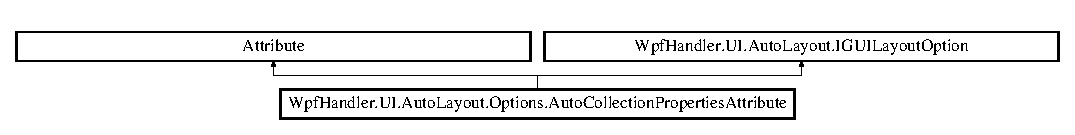
\includegraphics[height=1.372549cm]{d7/de8/class_wpf_handler_1_1_u_i_1_1_auto_layout_1_1_options_1_1_auto_collection_properties_attribute}
\end{center}
\end{figure}
\subsection*{Public Member Functions}
\begin{DoxyCompactItemize}
\item 
void \mbox{\hyperlink{class_wpf_handler_1_1_u_i_1_1_auto_layout_1_1_options_1_1_auto_collection_properties_attribute_aaff2195c793c7e75ac553291d9189655}{Apply\+Layout\+Option}} (Framework\+Element element)
\begin{DoxyCompactList}\small\item\em Applying collection properties to the elements if it\textquotesingle{}s inheirted from the Auto\+Collection \end{DoxyCompactList}\end{DoxyCompactItemize}
\subsection*{Properties}
\begin{DoxyCompactItemize}
\item 
double \mbox{\hyperlink{class_wpf_handler_1_1_u_i_1_1_auto_layout_1_1_options_1_1_auto_collection_properties_attribute_a7a137eb3059dd6d79f4edd9cee95769c}{Corner\+Radius}} = -\/1.\+0f\hspace{0.3cm}{\ttfamily  \mbox{[}get, set\mbox{]}}
\begin{DoxyCompactList}\small\item\em Radius of the rounded corders. Will affect default only if greater or equal to 0. \end{DoxyCompactList}\item 
bool \mbox{\hyperlink{class_wpf_handler_1_1_u_i_1_1_auto_layout_1_1_options_1_1_auto_collection_properties_attribute_a515d5509449af3cb2a46a770fb454778}{Spliters\+Draw}} = true\hspace{0.3cm}{\ttfamily  \mbox{[}get, set\mbox{]}}
\begin{DoxyCompactList}\small\item\em Is the spliting lines between content elements are visible. \end{DoxyCompactList}\item 
string \mbox{\hyperlink{class_wpf_handler_1_1_u_i_1_1_auto_layout_1_1_options_1_1_auto_collection_properties_attribute_a3d0bb6abd7d843bca5d6042e341dec7b}{Spliter\+Color}} = null\hspace{0.3cm}{\ttfamily  \mbox{[}get, set\mbox{]}}
\begin{DoxyCompactList}\small\item\em Color of the spliters. \end{DoxyCompactList}\item 
string \mbox{\hyperlink{class_wpf_handler_1_1_u_i_1_1_auto_layout_1_1_options_1_1_auto_collection_properties_attribute_a88ab71f9762a0d8425ebf57f72c0b2aa}{Backplate\+Background}} = null\hspace{0.3cm}{\ttfamily  \mbox{[}get, set\mbox{]}}
\begin{DoxyCompactList}\small\item\em Color of the backplate. \end{DoxyCompactList}\item 
bool \mbox{\hyperlink{class_wpf_handler_1_1_u_i_1_1_auto_layout_1_1_options_1_1_auto_collection_properties_attribute_aa93230d17f835aa86a64d12914ac482e}{Add\+Button\+Visibile}} = true\hspace{0.3cm}{\ttfamily  \mbox{[}get, set\mbox{]}}
\begin{DoxyCompactList}\small\item\em If the add button available for an user. \end{DoxyCompactList}\item 
bool \mbox{\hyperlink{class_wpf_handler_1_1_u_i_1_1_auto_layout_1_1_options_1_1_auto_collection_properties_attribute_a143a7de08e82032c232df0d05c2e1678}{Remove\+Button\+Visibile}} = true\hspace{0.3cm}{\ttfamily  \mbox{[}get, set\mbox{]}}
\begin{DoxyCompactList}\small\item\em Is the remove button available for an user. \end{DoxyCompactList}\item 
bool \mbox{\hyperlink{class_wpf_handler_1_1_u_i_1_1_auto_layout_1_1_options_1_1_auto_collection_properties_attribute_af5ff32848512ac0fb040b7e0d6311c0e}{Drag\+Allowed}} = true\hspace{0.3cm}{\ttfamily  \mbox{[}get, set\mbox{]}}
\begin{DoxyCompactList}\small\item\em Is the drag of elements allowed. \end{DoxyCompactList}\end{DoxyCompactItemize}


\subsection{Detailed Description}
Redefines default properties values for a Auto\+Collection control. Not affect any other controls. 



\subsection{Member Function Documentation}
\mbox{\Hypertarget{class_wpf_handler_1_1_u_i_1_1_auto_layout_1_1_options_1_1_auto_collection_properties_attribute_aaff2195c793c7e75ac553291d9189655}\label{class_wpf_handler_1_1_u_i_1_1_auto_layout_1_1_options_1_1_auto_collection_properties_attribute_aaff2195c793c7e75ac553291d9189655}} 
\index{Wpf\+Handler\+::\+U\+I\+::\+Auto\+Layout\+::\+Options\+::\+Auto\+Collection\+Properties\+Attribute@{Wpf\+Handler\+::\+U\+I\+::\+Auto\+Layout\+::\+Options\+::\+Auto\+Collection\+Properties\+Attribute}!Apply\+Layout\+Option@{Apply\+Layout\+Option}}
\index{Apply\+Layout\+Option@{Apply\+Layout\+Option}!Wpf\+Handler\+::\+U\+I\+::\+Auto\+Layout\+::\+Options\+::\+Auto\+Collection\+Properties\+Attribute@{Wpf\+Handler\+::\+U\+I\+::\+Auto\+Layout\+::\+Options\+::\+Auto\+Collection\+Properties\+Attribute}}
\subsubsection{\texorpdfstring{Apply\+Layout\+Option()}{ApplyLayoutOption()}}
{\footnotesize\ttfamily void Wpf\+Handler.\+U\+I.\+Auto\+Layout.\+Options.\+Auto\+Collection\+Properties\+Attribute.\+Apply\+Layout\+Option (\begin{DoxyParamCaption}\item[{Framework\+Element}]{element }\end{DoxyParamCaption})}



Applying collection properties to the elements if it\textquotesingle{}s inheirted from the Auto\+Collection 


\begin{DoxyParams}{Parameters}
{\em element} & The target \mbox{\hyperlink{namespace_wpf_handler_1_1_u_i}{UI}} element.\\
\hline
\end{DoxyParams}


Not causing an error if applying to element with a different type. 

Implements \mbox{\hyperlink{interface_wpf_handler_1_1_u_i_1_1_auto_layout_1_1_i_g_u_i_layout_option_ac2d2fa8aeaf753b3248381399f991005}{Wpf\+Handler.\+U\+I.\+Auto\+Layout.\+I\+G\+U\+I\+Layout\+Option}}.



\subsection{Property Documentation}
\mbox{\Hypertarget{class_wpf_handler_1_1_u_i_1_1_auto_layout_1_1_options_1_1_auto_collection_properties_attribute_aa93230d17f835aa86a64d12914ac482e}\label{class_wpf_handler_1_1_u_i_1_1_auto_layout_1_1_options_1_1_auto_collection_properties_attribute_aa93230d17f835aa86a64d12914ac482e}} 
\index{Wpf\+Handler\+::\+U\+I\+::\+Auto\+Layout\+::\+Options\+::\+Auto\+Collection\+Properties\+Attribute@{Wpf\+Handler\+::\+U\+I\+::\+Auto\+Layout\+::\+Options\+::\+Auto\+Collection\+Properties\+Attribute}!Add\+Button\+Visibile@{Add\+Button\+Visibile}}
\index{Add\+Button\+Visibile@{Add\+Button\+Visibile}!Wpf\+Handler\+::\+U\+I\+::\+Auto\+Layout\+::\+Options\+::\+Auto\+Collection\+Properties\+Attribute@{Wpf\+Handler\+::\+U\+I\+::\+Auto\+Layout\+::\+Options\+::\+Auto\+Collection\+Properties\+Attribute}}
\subsubsection{\texorpdfstring{Add\+Button\+Visibile}{AddButtonVisibile}}
{\footnotesize\ttfamily bool Wpf\+Handler.\+U\+I.\+Auto\+Layout.\+Options.\+Auto\+Collection\+Properties\+Attribute.\+Add\+Button\+Visibile = true\hspace{0.3cm}{\ttfamily [get]}, {\ttfamily [set]}}



If the add button available for an user. 

\mbox{\Hypertarget{class_wpf_handler_1_1_u_i_1_1_auto_layout_1_1_options_1_1_auto_collection_properties_attribute_a88ab71f9762a0d8425ebf57f72c0b2aa}\label{class_wpf_handler_1_1_u_i_1_1_auto_layout_1_1_options_1_1_auto_collection_properties_attribute_a88ab71f9762a0d8425ebf57f72c0b2aa}} 
\index{Wpf\+Handler\+::\+U\+I\+::\+Auto\+Layout\+::\+Options\+::\+Auto\+Collection\+Properties\+Attribute@{Wpf\+Handler\+::\+U\+I\+::\+Auto\+Layout\+::\+Options\+::\+Auto\+Collection\+Properties\+Attribute}!Backplate\+Background@{Backplate\+Background}}
\index{Backplate\+Background@{Backplate\+Background}!Wpf\+Handler\+::\+U\+I\+::\+Auto\+Layout\+::\+Options\+::\+Auto\+Collection\+Properties\+Attribute@{Wpf\+Handler\+::\+U\+I\+::\+Auto\+Layout\+::\+Options\+::\+Auto\+Collection\+Properties\+Attribute}}
\subsubsection{\texorpdfstring{Backplate\+Background}{BackplateBackground}}
{\footnotesize\ttfamily string Wpf\+Handler.\+U\+I.\+Auto\+Layout.\+Options.\+Auto\+Collection\+Properties\+Attribute.\+Backplate\+Background = null\hspace{0.3cm}{\ttfamily [get]}, {\ttfamily [set]}}



Color of the backplate. 

\mbox{\Hypertarget{class_wpf_handler_1_1_u_i_1_1_auto_layout_1_1_options_1_1_auto_collection_properties_attribute_a7a137eb3059dd6d79f4edd9cee95769c}\label{class_wpf_handler_1_1_u_i_1_1_auto_layout_1_1_options_1_1_auto_collection_properties_attribute_a7a137eb3059dd6d79f4edd9cee95769c}} 
\index{Wpf\+Handler\+::\+U\+I\+::\+Auto\+Layout\+::\+Options\+::\+Auto\+Collection\+Properties\+Attribute@{Wpf\+Handler\+::\+U\+I\+::\+Auto\+Layout\+::\+Options\+::\+Auto\+Collection\+Properties\+Attribute}!Corner\+Radius@{Corner\+Radius}}
\index{Corner\+Radius@{Corner\+Radius}!Wpf\+Handler\+::\+U\+I\+::\+Auto\+Layout\+::\+Options\+::\+Auto\+Collection\+Properties\+Attribute@{Wpf\+Handler\+::\+U\+I\+::\+Auto\+Layout\+::\+Options\+::\+Auto\+Collection\+Properties\+Attribute}}
\subsubsection{\texorpdfstring{Corner\+Radius}{CornerRadius}}
{\footnotesize\ttfamily double Wpf\+Handler.\+U\+I.\+Auto\+Layout.\+Options.\+Auto\+Collection\+Properties\+Attribute.\+Corner\+Radius = -\/1.\+0f\hspace{0.3cm}{\ttfamily [get]}, {\ttfamily [set]}}



Radius of the rounded corders. Will affect default only if greater or equal to 0. 

\mbox{\Hypertarget{class_wpf_handler_1_1_u_i_1_1_auto_layout_1_1_options_1_1_auto_collection_properties_attribute_af5ff32848512ac0fb040b7e0d6311c0e}\label{class_wpf_handler_1_1_u_i_1_1_auto_layout_1_1_options_1_1_auto_collection_properties_attribute_af5ff32848512ac0fb040b7e0d6311c0e}} 
\index{Wpf\+Handler\+::\+U\+I\+::\+Auto\+Layout\+::\+Options\+::\+Auto\+Collection\+Properties\+Attribute@{Wpf\+Handler\+::\+U\+I\+::\+Auto\+Layout\+::\+Options\+::\+Auto\+Collection\+Properties\+Attribute}!Drag\+Allowed@{Drag\+Allowed}}
\index{Drag\+Allowed@{Drag\+Allowed}!Wpf\+Handler\+::\+U\+I\+::\+Auto\+Layout\+::\+Options\+::\+Auto\+Collection\+Properties\+Attribute@{Wpf\+Handler\+::\+U\+I\+::\+Auto\+Layout\+::\+Options\+::\+Auto\+Collection\+Properties\+Attribute}}
\subsubsection{\texorpdfstring{Drag\+Allowed}{DragAllowed}}
{\footnotesize\ttfamily bool Wpf\+Handler.\+U\+I.\+Auto\+Layout.\+Options.\+Auto\+Collection\+Properties\+Attribute.\+Drag\+Allowed = true\hspace{0.3cm}{\ttfamily [get]}, {\ttfamily [set]}}



Is the drag of elements allowed. 

\mbox{\Hypertarget{class_wpf_handler_1_1_u_i_1_1_auto_layout_1_1_options_1_1_auto_collection_properties_attribute_a143a7de08e82032c232df0d05c2e1678}\label{class_wpf_handler_1_1_u_i_1_1_auto_layout_1_1_options_1_1_auto_collection_properties_attribute_a143a7de08e82032c232df0d05c2e1678}} 
\index{Wpf\+Handler\+::\+U\+I\+::\+Auto\+Layout\+::\+Options\+::\+Auto\+Collection\+Properties\+Attribute@{Wpf\+Handler\+::\+U\+I\+::\+Auto\+Layout\+::\+Options\+::\+Auto\+Collection\+Properties\+Attribute}!Remove\+Button\+Visibile@{Remove\+Button\+Visibile}}
\index{Remove\+Button\+Visibile@{Remove\+Button\+Visibile}!Wpf\+Handler\+::\+U\+I\+::\+Auto\+Layout\+::\+Options\+::\+Auto\+Collection\+Properties\+Attribute@{Wpf\+Handler\+::\+U\+I\+::\+Auto\+Layout\+::\+Options\+::\+Auto\+Collection\+Properties\+Attribute}}
\subsubsection{\texorpdfstring{Remove\+Button\+Visibile}{RemoveButtonVisibile}}
{\footnotesize\ttfamily bool Wpf\+Handler.\+U\+I.\+Auto\+Layout.\+Options.\+Auto\+Collection\+Properties\+Attribute.\+Remove\+Button\+Visibile = true\hspace{0.3cm}{\ttfamily [get]}, {\ttfamily [set]}}



Is the remove button available for an user. 

\mbox{\Hypertarget{class_wpf_handler_1_1_u_i_1_1_auto_layout_1_1_options_1_1_auto_collection_properties_attribute_a3d0bb6abd7d843bca5d6042e341dec7b}\label{class_wpf_handler_1_1_u_i_1_1_auto_layout_1_1_options_1_1_auto_collection_properties_attribute_a3d0bb6abd7d843bca5d6042e341dec7b}} 
\index{Wpf\+Handler\+::\+U\+I\+::\+Auto\+Layout\+::\+Options\+::\+Auto\+Collection\+Properties\+Attribute@{Wpf\+Handler\+::\+U\+I\+::\+Auto\+Layout\+::\+Options\+::\+Auto\+Collection\+Properties\+Attribute}!Spliter\+Color@{Spliter\+Color}}
\index{Spliter\+Color@{Spliter\+Color}!Wpf\+Handler\+::\+U\+I\+::\+Auto\+Layout\+::\+Options\+::\+Auto\+Collection\+Properties\+Attribute@{Wpf\+Handler\+::\+U\+I\+::\+Auto\+Layout\+::\+Options\+::\+Auto\+Collection\+Properties\+Attribute}}
\subsubsection{\texorpdfstring{Spliter\+Color}{SpliterColor}}
{\footnotesize\ttfamily string Wpf\+Handler.\+U\+I.\+Auto\+Layout.\+Options.\+Auto\+Collection\+Properties\+Attribute.\+Spliter\+Color = null\hspace{0.3cm}{\ttfamily [get]}, {\ttfamily [set]}}



Color of the spliters. 

\mbox{\Hypertarget{class_wpf_handler_1_1_u_i_1_1_auto_layout_1_1_options_1_1_auto_collection_properties_attribute_a515d5509449af3cb2a46a770fb454778}\label{class_wpf_handler_1_1_u_i_1_1_auto_layout_1_1_options_1_1_auto_collection_properties_attribute_a515d5509449af3cb2a46a770fb454778}} 
\index{Wpf\+Handler\+::\+U\+I\+::\+Auto\+Layout\+::\+Options\+::\+Auto\+Collection\+Properties\+Attribute@{Wpf\+Handler\+::\+U\+I\+::\+Auto\+Layout\+::\+Options\+::\+Auto\+Collection\+Properties\+Attribute}!Spliters\+Draw@{Spliters\+Draw}}
\index{Spliters\+Draw@{Spliters\+Draw}!Wpf\+Handler\+::\+U\+I\+::\+Auto\+Layout\+::\+Options\+::\+Auto\+Collection\+Properties\+Attribute@{Wpf\+Handler\+::\+U\+I\+::\+Auto\+Layout\+::\+Options\+::\+Auto\+Collection\+Properties\+Attribute}}
\subsubsection{\texorpdfstring{Spliters\+Draw}{SplitersDraw}}
{\footnotesize\ttfamily bool Wpf\+Handler.\+U\+I.\+Auto\+Layout.\+Options.\+Auto\+Collection\+Properties\+Attribute.\+Spliters\+Draw = true\hspace{0.3cm}{\ttfamily [get]}, {\ttfamily [set]}}



Is the spliting lines between content elements are visible. 



The documentation for this class was generated from the following file\+:\begin{DoxyCompactItemize}
\item 
D\+:/\+Work/\+Git\+Hub/wpf-\/handler/\+Wpf\+Handler/\+U\+I/\+Auto\+Layout/\+Options/Auto\+Collection\+Properties\+Attribute.\+cs\end{DoxyCompactItemize}

\hypertarget{class_wpf_handler_1_1_u_i_1_1_auto_layout_1_1_controls_1_1_auto_layout_veiw}{}\section{Wpf\+Handler.\+U\+I.\+Auto\+Layout.\+Controls.\+Auto\+Layout\+Veiw Class Reference}
\label{class_wpf_handler_1_1_u_i_1_1_auto_layout_1_1_controls_1_1_auto_layout_veiw}\index{Wpf\+Handler.\+U\+I.\+Auto\+Layout.\+Controls.\+Auto\+Layout\+Veiw@{Wpf\+Handler.\+U\+I.\+Auto\+Layout.\+Controls.\+Auto\+Layout\+Veiw}}


\mbox{\hyperlink{class_wpf_handler_1_1_u_i_1_1_auto_layout_1_1_controls_1_1_auto_layout_veiw}{Auto\+Layout\+Veiw}}  


Inheritance diagram for Wpf\+Handler.\+U\+I.\+Auto\+Layout.\+Controls.\+Auto\+Layout\+Veiw\+:\begin{figure}[H]
\begin{center}
\leavevmode
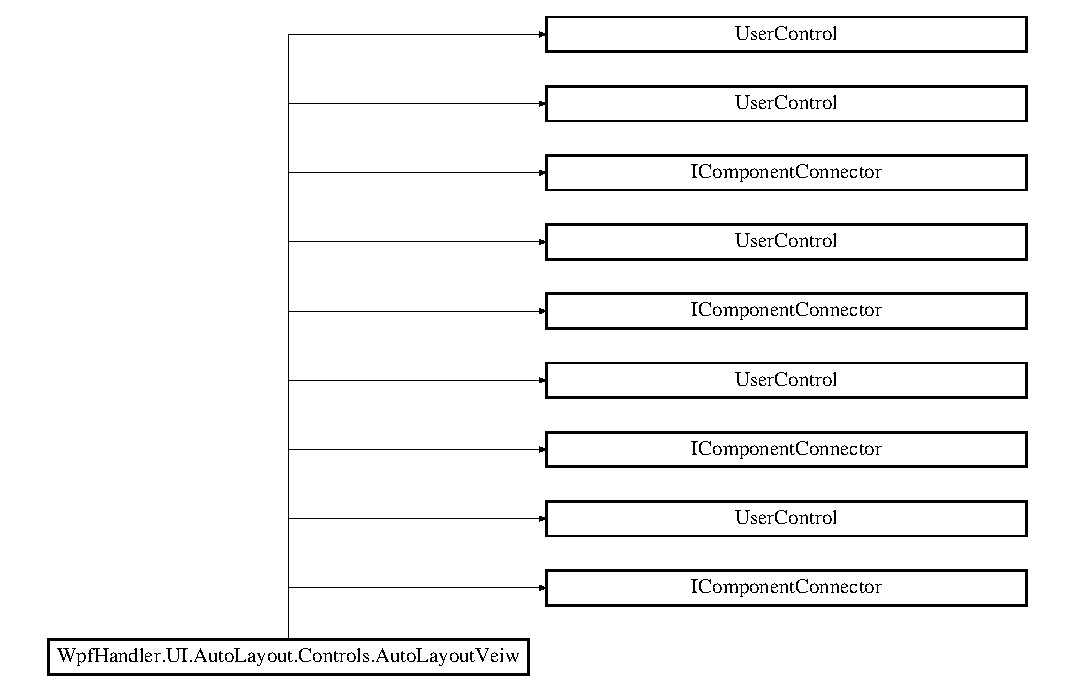
\includegraphics[height=8.832808cm]{d5/ddb/class_wpf_handler_1_1_u_i_1_1_auto_layout_1_1_controls_1_1_auto_layout_veiw}
\end{center}
\end{figure}
\subsection*{Public Member Functions}
\begin{DoxyCompactItemize}
\item 
void \mbox{\hyperlink{class_wpf_handler_1_1_u_i_1_1_auto_layout_1_1_controls_1_1_auto_layout_veiw_a9f1091c6f4daf3c752f2787d8ae1a4b6}{Initialize\+Component}} ()
\begin{DoxyCompactList}\small\item\em Initialize\+Component \end{DoxyCompactList}\item 
void \mbox{\hyperlink{class_wpf_handler_1_1_u_i_1_1_auto_layout_1_1_controls_1_1_auto_layout_veiw_a9f1091c6f4daf3c752f2787d8ae1a4b6}{Initialize\+Component}} ()
\begin{DoxyCompactList}\small\item\em Initialize\+Component \end{DoxyCompactList}\item 
void \mbox{\hyperlink{class_wpf_handler_1_1_u_i_1_1_auto_layout_1_1_controls_1_1_auto_layout_veiw_a9f1091c6f4daf3c752f2787d8ae1a4b6}{Initialize\+Component}} ()
\begin{DoxyCompactList}\small\item\em Initialize\+Component \end{DoxyCompactList}\item 
void \mbox{\hyperlink{class_wpf_handler_1_1_u_i_1_1_auto_layout_1_1_controls_1_1_auto_layout_veiw_a9f1091c6f4daf3c752f2787d8ae1a4b6}{Initialize\+Component}} ()
\begin{DoxyCompactList}\small\item\em Initialize\+Component \end{DoxyCompactList}\item 
\mbox{\hyperlink{class_wpf_handler_1_1_u_i_1_1_auto_layout_1_1_controls_1_1_auto_layout_veiw_a1bfcdfad104151ab6060168e0cbd0623}{Auto\+Layout\+Veiw}} ()
\begin{DoxyCompactList}\small\item\em Initialize component. \end{DoxyCompactList}\end{DoxyCompactItemize}
\subsection*{Protected Attributes}
\begin{DoxyCompactItemize}
\item 
\mbox{\hyperlink{class_wpf_handler_1_1_u_i_1_1_auto_layout_1_1_u_i_descriptor}{U\+I\+Descriptor}} \mbox{\hyperlink{class_wpf_handler_1_1_u_i_1_1_auto_layout_1_1_controls_1_1_auto_layout_veiw_abbafb7ec000393dc0cbffd3c1f1a8239}{\+\_\+\+Descriptor}}
\begin{DoxyCompactList}\small\item\em B\+Ufer that contains connected descriptor. \end{DoxyCompactList}\end{DoxyCompactItemize}
\subsection*{Package Attributes}
\begin{DoxyCompactItemize}
\item 
\mbox{\Hypertarget{class_wpf_handler_1_1_u_i_1_1_auto_layout_1_1_controls_1_1_auto_layout_veiw_a40493f222d9ffcdd653b767b68c52a44}\label{class_wpf_handler_1_1_u_i_1_1_auto_layout_1_1_controls_1_1_auto_layout_veiw_a40493f222d9ffcdd653b767b68c52a44}} 
\mbox{\hyperlink{class_wpf_handler_1_1_u_i_1_1_auto_layout_1_1_controls_1_1_auto_layout_veiw}{Wpf\+Handler.\+U\+I.\+Auto\+Layout.\+Controls.\+Auto\+Layout\+Veiw}} {\bfseries main}
\item 
\mbox{\Hypertarget{class_wpf_handler_1_1_u_i_1_1_auto_layout_1_1_controls_1_1_auto_layout_veiw_a7918966372bf9bad5dd25c837b748517}\label{class_wpf_handler_1_1_u_i_1_1_auto_layout_1_1_controls_1_1_auto_layout_veiw_a7918966372bf9bad5dd25c837b748517}} 
System.\+Windows.\+Controls.\+Stack\+Panel {\bfseries root}
\end{DoxyCompactItemize}
\subsection*{Properties}
\begin{DoxyCompactItemize}
\item 
\mbox{\hyperlink{class_wpf_handler_1_1_u_i_1_1_auto_layout_1_1_u_i_descriptor}{U\+I\+Descriptor}} \mbox{\hyperlink{class_wpf_handler_1_1_u_i_1_1_auto_layout_1_1_controls_1_1_auto_layout_veiw_abd1e3e95a1ed31eb35a7c6a531f51588}{Descriptor}}\hspace{0.3cm}{\ttfamily  \mbox{[}get, set\mbox{]}}
\begin{DoxyCompactList}\small\item\em Descriptor binded to the view. \end{DoxyCompactList}\end{DoxyCompactItemize}
\subsection*{Private Member Functions}
\begin{DoxyCompactItemize}
\item 
\mbox{\Hypertarget{class_wpf_handler_1_1_u_i_1_1_auto_layout_1_1_controls_1_1_auto_layout_veiw_af70d3c35cfef9f3e0c611ef4f01fcf35}\label{class_wpf_handler_1_1_u_i_1_1_auto_layout_1_1_controls_1_1_auto_layout_veiw_af70d3c35cfef9f3e0c611ef4f01fcf35}} 
void System.\+Windows.\+Markup.\+I\+Component\+Connector. {\bfseries Connect} (int connection\+Id, object target)
\item 
\mbox{\Hypertarget{class_wpf_handler_1_1_u_i_1_1_auto_layout_1_1_controls_1_1_auto_layout_veiw_af70d3c35cfef9f3e0c611ef4f01fcf35}\label{class_wpf_handler_1_1_u_i_1_1_auto_layout_1_1_controls_1_1_auto_layout_veiw_af70d3c35cfef9f3e0c611ef4f01fcf35}} 
void System.\+Windows.\+Markup.\+I\+Component\+Connector. {\bfseries Connect} (int connection\+Id, object target)
\item 
\mbox{\Hypertarget{class_wpf_handler_1_1_u_i_1_1_auto_layout_1_1_controls_1_1_auto_layout_veiw_af70d3c35cfef9f3e0c611ef4f01fcf35}\label{class_wpf_handler_1_1_u_i_1_1_auto_layout_1_1_controls_1_1_auto_layout_veiw_af70d3c35cfef9f3e0c611ef4f01fcf35}} 
void System.\+Windows.\+Markup.\+I\+Component\+Connector. {\bfseries Connect} (int connection\+Id, object target)
\item 
\mbox{\Hypertarget{class_wpf_handler_1_1_u_i_1_1_auto_layout_1_1_controls_1_1_auto_layout_veiw_af70d3c35cfef9f3e0c611ef4f01fcf35}\label{class_wpf_handler_1_1_u_i_1_1_auto_layout_1_1_controls_1_1_auto_layout_veiw_af70d3c35cfef9f3e0c611ef4f01fcf35}} 
void System.\+Windows.\+Markup.\+I\+Component\+Connector. {\bfseries Connect} (int connection\+Id, object target)
\item 
\mbox{\hyperlink{class_wpf_handler_1_1_u_i_1_1_auto_layout_1_1_controls_1_1_auto_layout_veiw_a1a6e98c4dc79f492b2174080f07c6705}{$\sim$\+Auto\+Layout\+Veiw}} ()
\begin{DoxyCompactList}\small\item\em Releasing unmanaged memory. \end{DoxyCompactList}\item 
void \mbox{\hyperlink{class_wpf_handler_1_1_u_i_1_1_auto_layout_1_1_controls_1_1_auto_layout_veiw_a651648035cd4ac0e459c8cf1daa81116}{Main\+\_\+\+Loaded}} (object sender, Routed\+Event\+Args e)
\begin{DoxyCompactList}\small\item\em Update dat after loading. \end{DoxyCompactList}\end{DoxyCompactItemize}
\subsection*{Private Attributes}
\begin{DoxyCompactItemize}
\item 
\mbox{\Hypertarget{class_wpf_handler_1_1_u_i_1_1_auto_layout_1_1_controls_1_1_auto_layout_veiw_aee334a65367c5ca61fb4bf3bff5e72d0}\label{class_wpf_handler_1_1_u_i_1_1_auto_layout_1_1_controls_1_1_auto_layout_veiw_aee334a65367c5ca61fb4bf3bff5e72d0}} 
bool {\bfseries \+\_\+content\+Loaded}
\end{DoxyCompactItemize}


\subsection{Detailed Description}
\mbox{\hyperlink{class_wpf_handler_1_1_u_i_1_1_auto_layout_1_1_controls_1_1_auto_layout_veiw}{Auto\+Layout\+Veiw}} 

Allow to connect auto generated G\+UI to the X\+A\+ML descriptor. 

\subsection{Constructor \& Destructor Documentation}
\mbox{\Hypertarget{class_wpf_handler_1_1_u_i_1_1_auto_layout_1_1_controls_1_1_auto_layout_veiw_a1bfcdfad104151ab6060168e0cbd0623}\label{class_wpf_handler_1_1_u_i_1_1_auto_layout_1_1_controls_1_1_auto_layout_veiw_a1bfcdfad104151ab6060168e0cbd0623}} 
\index{Wpf\+Handler\+::\+U\+I\+::\+Auto\+Layout\+::\+Controls\+::\+Auto\+Layout\+Veiw@{Wpf\+Handler\+::\+U\+I\+::\+Auto\+Layout\+::\+Controls\+::\+Auto\+Layout\+Veiw}!Auto\+Layout\+Veiw@{Auto\+Layout\+Veiw}}
\index{Auto\+Layout\+Veiw@{Auto\+Layout\+Veiw}!Wpf\+Handler\+::\+U\+I\+::\+Auto\+Layout\+::\+Controls\+::\+Auto\+Layout\+Veiw@{Wpf\+Handler\+::\+U\+I\+::\+Auto\+Layout\+::\+Controls\+::\+Auto\+Layout\+Veiw}}
\subsubsection{\texorpdfstring{Auto\+Layout\+Veiw()}{AutoLayoutVeiw()}}
{\footnotesize\ttfamily Wpf\+Handler.\+U\+I.\+Auto\+Layout.\+Controls.\+Auto\+Layout\+Veiw.\+Auto\+Layout\+Veiw (\begin{DoxyParamCaption}{ }\end{DoxyParamCaption})}



Initialize component. 

\mbox{\Hypertarget{class_wpf_handler_1_1_u_i_1_1_auto_layout_1_1_controls_1_1_auto_layout_veiw_a1a6e98c4dc79f492b2174080f07c6705}\label{class_wpf_handler_1_1_u_i_1_1_auto_layout_1_1_controls_1_1_auto_layout_veiw_a1a6e98c4dc79f492b2174080f07c6705}} 
\index{Wpf\+Handler\+::\+U\+I\+::\+Auto\+Layout\+::\+Controls\+::\+Auto\+Layout\+Veiw@{Wpf\+Handler\+::\+U\+I\+::\+Auto\+Layout\+::\+Controls\+::\+Auto\+Layout\+Veiw}!````~Auto\+Layout\+Veiw@{$\sim$\+Auto\+Layout\+Veiw}}
\index{````~Auto\+Layout\+Veiw@{$\sim$\+Auto\+Layout\+Veiw}!Wpf\+Handler\+::\+U\+I\+::\+Auto\+Layout\+::\+Controls\+::\+Auto\+Layout\+Veiw@{Wpf\+Handler\+::\+U\+I\+::\+Auto\+Layout\+::\+Controls\+::\+Auto\+Layout\+Veiw}}
\subsubsection{\texorpdfstring{$\sim$\+Auto\+Layout\+Veiw()}{~AutoLayoutVeiw()}}
{\footnotesize\ttfamily Wpf\+Handler.\+U\+I.\+Auto\+Layout.\+Controls.\+Auto\+Layout\+Veiw.$\sim$\+Auto\+Layout\+Veiw (\begin{DoxyParamCaption}{ }\end{DoxyParamCaption})\hspace{0.3cm}{\ttfamily [private]}}



Releasing unmanaged memory. 



\subsection{Member Function Documentation}
\mbox{\Hypertarget{class_wpf_handler_1_1_u_i_1_1_auto_layout_1_1_controls_1_1_auto_layout_veiw_a9f1091c6f4daf3c752f2787d8ae1a4b6}\label{class_wpf_handler_1_1_u_i_1_1_auto_layout_1_1_controls_1_1_auto_layout_veiw_a9f1091c6f4daf3c752f2787d8ae1a4b6}} 
\index{Wpf\+Handler\+::\+U\+I\+::\+Auto\+Layout\+::\+Controls\+::\+Auto\+Layout\+Veiw@{Wpf\+Handler\+::\+U\+I\+::\+Auto\+Layout\+::\+Controls\+::\+Auto\+Layout\+Veiw}!Initialize\+Component@{Initialize\+Component}}
\index{Initialize\+Component@{Initialize\+Component}!Wpf\+Handler\+::\+U\+I\+::\+Auto\+Layout\+::\+Controls\+::\+Auto\+Layout\+Veiw@{Wpf\+Handler\+::\+U\+I\+::\+Auto\+Layout\+::\+Controls\+::\+Auto\+Layout\+Veiw}}
\subsubsection{\texorpdfstring{Initialize\+Component()}{InitializeComponent()}\hspace{0.1cm}{\footnotesize\ttfamily [1/4]}}
{\footnotesize\ttfamily void Wpf\+Handler.\+U\+I.\+Auto\+Layout.\+Controls.\+Auto\+Layout\+Veiw.\+Initialize\+Component (\begin{DoxyParamCaption}{ }\end{DoxyParamCaption})}



Initialize\+Component 

\mbox{\Hypertarget{class_wpf_handler_1_1_u_i_1_1_auto_layout_1_1_controls_1_1_auto_layout_veiw_a9f1091c6f4daf3c752f2787d8ae1a4b6}\label{class_wpf_handler_1_1_u_i_1_1_auto_layout_1_1_controls_1_1_auto_layout_veiw_a9f1091c6f4daf3c752f2787d8ae1a4b6}} 
\index{Wpf\+Handler\+::\+U\+I\+::\+Auto\+Layout\+::\+Controls\+::\+Auto\+Layout\+Veiw@{Wpf\+Handler\+::\+U\+I\+::\+Auto\+Layout\+::\+Controls\+::\+Auto\+Layout\+Veiw}!Initialize\+Component@{Initialize\+Component}}
\index{Initialize\+Component@{Initialize\+Component}!Wpf\+Handler\+::\+U\+I\+::\+Auto\+Layout\+::\+Controls\+::\+Auto\+Layout\+Veiw@{Wpf\+Handler\+::\+U\+I\+::\+Auto\+Layout\+::\+Controls\+::\+Auto\+Layout\+Veiw}}
\subsubsection{\texorpdfstring{Initialize\+Component()}{InitializeComponent()}\hspace{0.1cm}{\footnotesize\ttfamily [2/4]}}
{\footnotesize\ttfamily void Wpf\+Handler.\+U\+I.\+Auto\+Layout.\+Controls.\+Auto\+Layout\+Veiw.\+Initialize\+Component (\begin{DoxyParamCaption}{ }\end{DoxyParamCaption})}



Initialize\+Component 

\mbox{\Hypertarget{class_wpf_handler_1_1_u_i_1_1_auto_layout_1_1_controls_1_1_auto_layout_veiw_a9f1091c6f4daf3c752f2787d8ae1a4b6}\label{class_wpf_handler_1_1_u_i_1_1_auto_layout_1_1_controls_1_1_auto_layout_veiw_a9f1091c6f4daf3c752f2787d8ae1a4b6}} 
\index{Wpf\+Handler\+::\+U\+I\+::\+Auto\+Layout\+::\+Controls\+::\+Auto\+Layout\+Veiw@{Wpf\+Handler\+::\+U\+I\+::\+Auto\+Layout\+::\+Controls\+::\+Auto\+Layout\+Veiw}!Initialize\+Component@{Initialize\+Component}}
\index{Initialize\+Component@{Initialize\+Component}!Wpf\+Handler\+::\+U\+I\+::\+Auto\+Layout\+::\+Controls\+::\+Auto\+Layout\+Veiw@{Wpf\+Handler\+::\+U\+I\+::\+Auto\+Layout\+::\+Controls\+::\+Auto\+Layout\+Veiw}}
\subsubsection{\texorpdfstring{Initialize\+Component()}{InitializeComponent()}\hspace{0.1cm}{\footnotesize\ttfamily [3/4]}}
{\footnotesize\ttfamily void Wpf\+Handler.\+U\+I.\+Auto\+Layout.\+Controls.\+Auto\+Layout\+Veiw.\+Initialize\+Component (\begin{DoxyParamCaption}{ }\end{DoxyParamCaption})}



Initialize\+Component 

\mbox{\Hypertarget{class_wpf_handler_1_1_u_i_1_1_auto_layout_1_1_controls_1_1_auto_layout_veiw_a9f1091c6f4daf3c752f2787d8ae1a4b6}\label{class_wpf_handler_1_1_u_i_1_1_auto_layout_1_1_controls_1_1_auto_layout_veiw_a9f1091c6f4daf3c752f2787d8ae1a4b6}} 
\index{Wpf\+Handler\+::\+U\+I\+::\+Auto\+Layout\+::\+Controls\+::\+Auto\+Layout\+Veiw@{Wpf\+Handler\+::\+U\+I\+::\+Auto\+Layout\+::\+Controls\+::\+Auto\+Layout\+Veiw}!Initialize\+Component@{Initialize\+Component}}
\index{Initialize\+Component@{Initialize\+Component}!Wpf\+Handler\+::\+U\+I\+::\+Auto\+Layout\+::\+Controls\+::\+Auto\+Layout\+Veiw@{Wpf\+Handler\+::\+U\+I\+::\+Auto\+Layout\+::\+Controls\+::\+Auto\+Layout\+Veiw}}
\subsubsection{\texorpdfstring{Initialize\+Component()}{InitializeComponent()}\hspace{0.1cm}{\footnotesize\ttfamily [4/4]}}
{\footnotesize\ttfamily void Wpf\+Handler.\+U\+I.\+Auto\+Layout.\+Controls.\+Auto\+Layout\+Veiw.\+Initialize\+Component (\begin{DoxyParamCaption}{ }\end{DoxyParamCaption})}



Initialize\+Component 

\mbox{\Hypertarget{class_wpf_handler_1_1_u_i_1_1_auto_layout_1_1_controls_1_1_auto_layout_veiw_a651648035cd4ac0e459c8cf1daa81116}\label{class_wpf_handler_1_1_u_i_1_1_auto_layout_1_1_controls_1_1_auto_layout_veiw_a651648035cd4ac0e459c8cf1daa81116}} 
\index{Wpf\+Handler\+::\+U\+I\+::\+Auto\+Layout\+::\+Controls\+::\+Auto\+Layout\+Veiw@{Wpf\+Handler\+::\+U\+I\+::\+Auto\+Layout\+::\+Controls\+::\+Auto\+Layout\+Veiw}!Main\+\_\+\+Loaded@{Main\+\_\+\+Loaded}}
\index{Main\+\_\+\+Loaded@{Main\+\_\+\+Loaded}!Wpf\+Handler\+::\+U\+I\+::\+Auto\+Layout\+::\+Controls\+::\+Auto\+Layout\+Veiw@{Wpf\+Handler\+::\+U\+I\+::\+Auto\+Layout\+::\+Controls\+::\+Auto\+Layout\+Veiw}}
\subsubsection{\texorpdfstring{Main\+\_\+\+Loaded()}{Main\_Loaded()}}
{\footnotesize\ttfamily void Wpf\+Handler.\+U\+I.\+Auto\+Layout.\+Controls.\+Auto\+Layout\+Veiw.\+Main\+\_\+\+Loaded (\begin{DoxyParamCaption}\item[{object}]{sender,  }\item[{Routed\+Event\+Args}]{e }\end{DoxyParamCaption})\hspace{0.3cm}{\ttfamily [private]}}



Update dat after loading. 


\begin{DoxyParams}{Parameters}
{\em sender} & \\
\hline
{\em e} & \\
\hline
\end{DoxyParams}


\subsection{Member Data Documentation}
\mbox{\Hypertarget{class_wpf_handler_1_1_u_i_1_1_auto_layout_1_1_controls_1_1_auto_layout_veiw_abbafb7ec000393dc0cbffd3c1f1a8239}\label{class_wpf_handler_1_1_u_i_1_1_auto_layout_1_1_controls_1_1_auto_layout_veiw_abbafb7ec000393dc0cbffd3c1f1a8239}} 
\index{Wpf\+Handler\+::\+U\+I\+::\+Auto\+Layout\+::\+Controls\+::\+Auto\+Layout\+Veiw@{Wpf\+Handler\+::\+U\+I\+::\+Auto\+Layout\+::\+Controls\+::\+Auto\+Layout\+Veiw}!\+\_\+\+Descriptor@{\+\_\+\+Descriptor}}
\index{\+\_\+\+Descriptor@{\+\_\+\+Descriptor}!Wpf\+Handler\+::\+U\+I\+::\+Auto\+Layout\+::\+Controls\+::\+Auto\+Layout\+Veiw@{Wpf\+Handler\+::\+U\+I\+::\+Auto\+Layout\+::\+Controls\+::\+Auto\+Layout\+Veiw}}
\subsubsection{\texorpdfstring{\+\_\+\+Descriptor}{\_Descriptor}}
{\footnotesize\ttfamily \mbox{\hyperlink{class_wpf_handler_1_1_u_i_1_1_auto_layout_1_1_u_i_descriptor}{U\+I\+Descriptor}} Wpf\+Handler.\+U\+I.\+Auto\+Layout.\+Controls.\+Auto\+Layout\+Veiw.\+\_\+\+Descriptor\hspace{0.3cm}{\ttfamily [protected]}}



B\+Ufer that contains connected descriptor. 



\subsection{Property Documentation}
\mbox{\Hypertarget{class_wpf_handler_1_1_u_i_1_1_auto_layout_1_1_controls_1_1_auto_layout_veiw_abd1e3e95a1ed31eb35a7c6a531f51588}\label{class_wpf_handler_1_1_u_i_1_1_auto_layout_1_1_controls_1_1_auto_layout_veiw_abd1e3e95a1ed31eb35a7c6a531f51588}} 
\index{Wpf\+Handler\+::\+U\+I\+::\+Auto\+Layout\+::\+Controls\+::\+Auto\+Layout\+Veiw@{Wpf\+Handler\+::\+U\+I\+::\+Auto\+Layout\+::\+Controls\+::\+Auto\+Layout\+Veiw}!Descriptor@{Descriptor}}
\index{Descriptor@{Descriptor}!Wpf\+Handler\+::\+U\+I\+::\+Auto\+Layout\+::\+Controls\+::\+Auto\+Layout\+Veiw@{Wpf\+Handler\+::\+U\+I\+::\+Auto\+Layout\+::\+Controls\+::\+Auto\+Layout\+Veiw}}
\subsubsection{\texorpdfstring{Descriptor}{Descriptor}}
{\footnotesize\ttfamily \mbox{\hyperlink{class_wpf_handler_1_1_u_i_1_1_auto_layout_1_1_u_i_descriptor}{U\+I\+Descriptor}} Wpf\+Handler.\+U\+I.\+Auto\+Layout.\+Controls.\+Auto\+Layout\+Veiw.\+Descriptor\hspace{0.3cm}{\ttfamily [get]}, {\ttfamily [set]}}



Descriptor binded to the view. 



The documentation for this class was generated from the following files\+:\begin{DoxyCompactItemize}
\item 
D\+:/\+Work/\+Git\+Hub/wpf-\/handler/\+Wpf\+Handler/obj/\+Debug/\+U\+I/\+Auto\+Layout/\+Controls/Auto\+Layout\+Veiw.\+g.\+cs\item 
D\+:/\+Work/\+Git\+Hub/wpf-\/handler/\+Wpf\+Handler/obj/\+Debug/\+U\+I/\+Auto\+Layout/\+Controls/Auto\+Layout\+Veiw.\+g.\+i.\+cs\item 
D\+:/\+Work/\+Git\+Hub/wpf-\/handler/\+Wpf\+Handler/\+U\+I/\+Auto\+Layout/\+Controls/Auto\+Layout\+Veiw.\+xaml.\+cs\end{DoxyCompactItemize}

\hypertarget{class_wpf_handler_1_1_u_i_1_1_auto_layout_1_1_options_1_1_background_attribute}{}\section{Wpf\+Handler.\+U\+I.\+Auto\+Layout.\+Options.\+Background\+Attribute Class Reference}
\label{class_wpf_handler_1_1_u_i_1_1_auto_layout_1_1_options_1_1_background_attribute}\index{Wpf\+Handler.\+U\+I.\+Auto\+Layout.\+Options.\+Background\+Attribute@{Wpf\+Handler.\+U\+I.\+Auto\+Layout.\+Options.\+Background\+Attribute}}


Define G\+UI element\textquotesingle{}s background brush.  


Inheritance diagram for Wpf\+Handler.\+U\+I.\+Auto\+Layout.\+Options.\+Background\+Attribute\+:\begin{figure}[H]
\begin{center}
\leavevmode
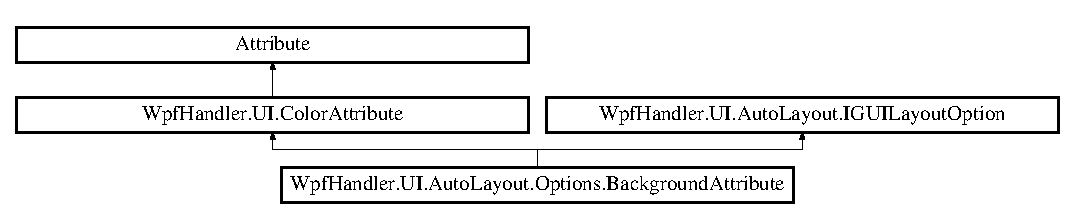
\includegraphics[height=2.500000cm]{d7/dde/class_wpf_handler_1_1_u_i_1_1_auto_layout_1_1_options_1_1_background_attribute}
\end{center}
\end{figure}
\subsection*{Public Member Functions}
\begin{DoxyCompactItemize}
\item 
\mbox{\hyperlink{class_wpf_handler_1_1_u_i_1_1_auto_layout_1_1_options_1_1_background_attribute_ade7defa6df0ce136497f5f8d617d645e}{Background\+Attribute}} (\mbox{\hyperlink{class_wpf_handler_1_1_u_i_1_1_color_attribute_afa14c4542d8023b3ddad6aba74993877}{Brush}} brush)
\begin{DoxyCompactList}\small\item\em Instiniating attribute with applied brush. \end{DoxyCompactList}\item 
\mbox{\hyperlink{class_wpf_handler_1_1_u_i_1_1_auto_layout_1_1_options_1_1_background_attribute_a5f31da6c168c956689ae1ef689bc2935}{Background\+Attribute}} (Solid\+Color\+Brush brush)
\begin{DoxyCompactList}\small\item\em Instiniating attribute with applied brush. \end{DoxyCompactList}\item 
\mbox{\hyperlink{class_wpf_handler_1_1_u_i_1_1_auto_layout_1_1_options_1_1_background_attribute_a47ce104c6fcb0fad6036dc109d1492eb}{Background\+Attribute}} (string color\+Code)
\begin{DoxyCompactList}\small\item\em Instiniating attribute with applied brush. \end{DoxyCompactList}\item 
\mbox{\hyperlink{class_wpf_handler_1_1_u_i_1_1_auto_layout_1_1_options_1_1_background_attribute_a2453a8f7be0ebe63191e01e6490052f8}{Background\+Attribute}} (\mbox{\hyperlink{class_wpf_handler_1_1_u_i_1_1_color_attribute_a6c5c2202427bd48877142ecf85327843}{Color}} color)
\begin{DoxyCompactList}\small\item\em Instiniating attribute with applied color. \end{DoxyCompactList}\item 
void \mbox{\hyperlink{class_wpf_handler_1_1_u_i_1_1_auto_layout_1_1_options_1_1_background_attribute_a97cce29c9e19d9145e881c69e3bf3d4e}{Apply\+Layout\+Option}} (Framework\+Element element)
\begin{DoxyCompactList}\small\item\em Define G\+UI element\textquotesingle{}s background brush. \end{DoxyCompactList}\end{DoxyCompactItemize}
\subsection*{Additional Inherited Members}


\subsection{Detailed Description}
Define G\+UI element\textquotesingle{}s background brush. 



\subsection{Constructor \& Destructor Documentation}
\mbox{\Hypertarget{class_wpf_handler_1_1_u_i_1_1_auto_layout_1_1_options_1_1_background_attribute_ade7defa6df0ce136497f5f8d617d645e}\label{class_wpf_handler_1_1_u_i_1_1_auto_layout_1_1_options_1_1_background_attribute_ade7defa6df0ce136497f5f8d617d645e}} 
\index{Wpf\+Handler\+::\+U\+I\+::\+Auto\+Layout\+::\+Options\+::\+Background\+Attribute@{Wpf\+Handler\+::\+U\+I\+::\+Auto\+Layout\+::\+Options\+::\+Background\+Attribute}!Background\+Attribute@{Background\+Attribute}}
\index{Background\+Attribute@{Background\+Attribute}!Wpf\+Handler\+::\+U\+I\+::\+Auto\+Layout\+::\+Options\+::\+Background\+Attribute@{Wpf\+Handler\+::\+U\+I\+::\+Auto\+Layout\+::\+Options\+::\+Background\+Attribute}}
\subsubsection{\texorpdfstring{Background\+Attribute()}{BackgroundAttribute()}\hspace{0.1cm}{\footnotesize\ttfamily [1/4]}}
{\footnotesize\ttfamily Wpf\+Handler.\+U\+I.\+Auto\+Layout.\+Options.\+Background\+Attribute.\+Background\+Attribute (\begin{DoxyParamCaption}\item[{\mbox{\hyperlink{class_wpf_handler_1_1_u_i_1_1_color_attribute_afa14c4542d8023b3ddad6aba74993877}{Brush}}}]{brush }\end{DoxyParamCaption})}



Instiniating attribute with applied brush. 


\begin{DoxyParams}{Parameters}
{\em brush} & Target brush.\\
\hline
\end{DoxyParams}


No supported via attribute.\mbox{\Hypertarget{class_wpf_handler_1_1_u_i_1_1_auto_layout_1_1_options_1_1_background_attribute_a5f31da6c168c956689ae1ef689bc2935}\label{class_wpf_handler_1_1_u_i_1_1_auto_layout_1_1_options_1_1_background_attribute_a5f31da6c168c956689ae1ef689bc2935}} 
\index{Wpf\+Handler\+::\+U\+I\+::\+Auto\+Layout\+::\+Options\+::\+Background\+Attribute@{Wpf\+Handler\+::\+U\+I\+::\+Auto\+Layout\+::\+Options\+::\+Background\+Attribute}!Background\+Attribute@{Background\+Attribute}}
\index{Background\+Attribute@{Background\+Attribute}!Wpf\+Handler\+::\+U\+I\+::\+Auto\+Layout\+::\+Options\+::\+Background\+Attribute@{Wpf\+Handler\+::\+U\+I\+::\+Auto\+Layout\+::\+Options\+::\+Background\+Attribute}}
\subsubsection{\texorpdfstring{Background\+Attribute()}{BackgroundAttribute()}\hspace{0.1cm}{\footnotesize\ttfamily [2/4]}}
{\footnotesize\ttfamily Wpf\+Handler.\+U\+I.\+Auto\+Layout.\+Options.\+Background\+Attribute.\+Background\+Attribute (\begin{DoxyParamCaption}\item[{Solid\+Color\+Brush}]{brush }\end{DoxyParamCaption})}



Instiniating attribute with applied brush. 


\begin{DoxyParams}{Parameters}
{\em brush} & Target brush.\\
\hline
\end{DoxyParams}


No supported via attribute.\mbox{\Hypertarget{class_wpf_handler_1_1_u_i_1_1_auto_layout_1_1_options_1_1_background_attribute_a47ce104c6fcb0fad6036dc109d1492eb}\label{class_wpf_handler_1_1_u_i_1_1_auto_layout_1_1_options_1_1_background_attribute_a47ce104c6fcb0fad6036dc109d1492eb}} 
\index{Wpf\+Handler\+::\+U\+I\+::\+Auto\+Layout\+::\+Options\+::\+Background\+Attribute@{Wpf\+Handler\+::\+U\+I\+::\+Auto\+Layout\+::\+Options\+::\+Background\+Attribute}!Background\+Attribute@{Background\+Attribute}}
\index{Background\+Attribute@{Background\+Attribute}!Wpf\+Handler\+::\+U\+I\+::\+Auto\+Layout\+::\+Options\+::\+Background\+Attribute@{Wpf\+Handler\+::\+U\+I\+::\+Auto\+Layout\+::\+Options\+::\+Background\+Attribute}}
\subsubsection{\texorpdfstring{Background\+Attribute()}{BackgroundAttribute()}\hspace{0.1cm}{\footnotesize\ttfamily [3/4]}}
{\footnotesize\ttfamily Wpf\+Handler.\+U\+I.\+Auto\+Layout.\+Options.\+Background\+Attribute.\+Background\+Attribute (\begin{DoxyParamCaption}\item[{string}]{color\+Code }\end{DoxyParamCaption})}



Instiniating attribute with applied brush. 


\begin{DoxyParams}{Parameters}
{\em color\+Code} & Trying to apply string color code as brush by using Color\+Converter rules. Not throw excption in case if color\textquotesingle{}s code invalid to prevent \mbox{\hyperlink{namespace_wpf_handler_1_1_u_i}{UI}} crash.\\
\hline
\end{DoxyParams}
\mbox{\Hypertarget{class_wpf_handler_1_1_u_i_1_1_auto_layout_1_1_options_1_1_background_attribute_a2453a8f7be0ebe63191e01e6490052f8}\label{class_wpf_handler_1_1_u_i_1_1_auto_layout_1_1_options_1_1_background_attribute_a2453a8f7be0ebe63191e01e6490052f8}} 
\index{Wpf\+Handler\+::\+U\+I\+::\+Auto\+Layout\+::\+Options\+::\+Background\+Attribute@{Wpf\+Handler\+::\+U\+I\+::\+Auto\+Layout\+::\+Options\+::\+Background\+Attribute}!Background\+Attribute@{Background\+Attribute}}
\index{Background\+Attribute@{Background\+Attribute}!Wpf\+Handler\+::\+U\+I\+::\+Auto\+Layout\+::\+Options\+::\+Background\+Attribute@{Wpf\+Handler\+::\+U\+I\+::\+Auto\+Layout\+::\+Options\+::\+Background\+Attribute}}
\subsubsection{\texorpdfstring{Background\+Attribute()}{BackgroundAttribute()}\hspace{0.1cm}{\footnotesize\ttfamily [4/4]}}
{\footnotesize\ttfamily Wpf\+Handler.\+U\+I.\+Auto\+Layout.\+Options.\+Background\+Attribute.\+Background\+Attribute (\begin{DoxyParamCaption}\item[{\mbox{\hyperlink{class_wpf_handler_1_1_u_i_1_1_color_attribute_a6c5c2202427bd48877142ecf85327843}{Color}}}]{color }\end{DoxyParamCaption})}



Instiniating attribute with applied color. 


\begin{DoxyParams}{Parameters}
{\em color} & Target color.\\
\hline
\end{DoxyParams}


No supported via attribute.

\subsection{Member Function Documentation}
\mbox{\Hypertarget{class_wpf_handler_1_1_u_i_1_1_auto_layout_1_1_options_1_1_background_attribute_a97cce29c9e19d9145e881c69e3bf3d4e}\label{class_wpf_handler_1_1_u_i_1_1_auto_layout_1_1_options_1_1_background_attribute_a97cce29c9e19d9145e881c69e3bf3d4e}} 
\index{Wpf\+Handler\+::\+U\+I\+::\+Auto\+Layout\+::\+Options\+::\+Background\+Attribute@{Wpf\+Handler\+::\+U\+I\+::\+Auto\+Layout\+::\+Options\+::\+Background\+Attribute}!Apply\+Layout\+Option@{Apply\+Layout\+Option}}
\index{Apply\+Layout\+Option@{Apply\+Layout\+Option}!Wpf\+Handler\+::\+U\+I\+::\+Auto\+Layout\+::\+Options\+::\+Background\+Attribute@{Wpf\+Handler\+::\+U\+I\+::\+Auto\+Layout\+::\+Options\+::\+Background\+Attribute}}
\subsubsection{\texorpdfstring{Apply\+Layout\+Option()}{ApplyLayoutOption()}}
{\footnotesize\ttfamily void Wpf\+Handler.\+U\+I.\+Auto\+Layout.\+Options.\+Background\+Attribute.\+Apply\+Layout\+Option (\begin{DoxyParamCaption}\item[{Framework\+Element}]{element }\end{DoxyParamCaption})}



Define G\+UI element\textquotesingle{}s background brush. 


\begin{DoxyParams}{Parameters}
{\em element} & Shared \mbox{\hyperlink{namespace_wpf_handler_1_1_u_i}{UI}} element. Must be inheirted from {\ttfamily System.\+Windows.\+Controls.\+Control} to affect the font properties. \\
\hline
\end{DoxyParams}


Implements \mbox{\hyperlink{interface_wpf_handler_1_1_u_i_1_1_auto_layout_1_1_i_g_u_i_layout_option_ac2d2fa8aeaf753b3248381399f991005}{Wpf\+Handler.\+U\+I.\+Auto\+Layout.\+I\+G\+U\+I\+Layout\+Option}}.



The documentation for this class was generated from the following file\+:\begin{DoxyCompactItemize}
\item 
D\+:/\+Work/\+Git\+Hub/wpf-\/handler/\+Wpf\+Handler/\+U\+I/\+Auto\+Layout/\+Options/Background\+Attribute.\+cs\end{DoxyCompactItemize}

\hypertarget{class_wpf_handler_1_1_u_i_1_1_auto_layout_1_1_configuration_1_1_begin_horizontal_group_attribute}{}\section{Wpf\+Handler.\+U\+I.\+Auto\+Layout.\+Configuration.\+Begin\+Horizontal\+Group\+Attribute Class Reference}
\label{class_wpf_handler_1_1_u_i_1_1_auto_layout_1_1_configuration_1_1_begin_horizontal_group_attribute}\index{Wpf\+Handler.\+U\+I.\+Auto\+Layout.\+Configuration.\+Begin\+Horizontal\+Group\+Attribute@{Wpf\+Handler.\+U\+I.\+Auto\+Layout.\+Configuration.\+Begin\+Horizontal\+Group\+Attribute}}


Starting a horizontal layout group. Will wait \mbox{\hyperlink{class_wpf_handler_1_1_u_i_1_1_auto_layout_1_1_configuration_1_1_end_group_attribute}{End\+Group\+Attribute}} to over the last begined group.  


Inheritance diagram for Wpf\+Handler.\+U\+I.\+Auto\+Layout.\+Configuration.\+Begin\+Horizontal\+Group\+Attribute\+:\begin{figure}[H]
\begin{center}
\leavevmode
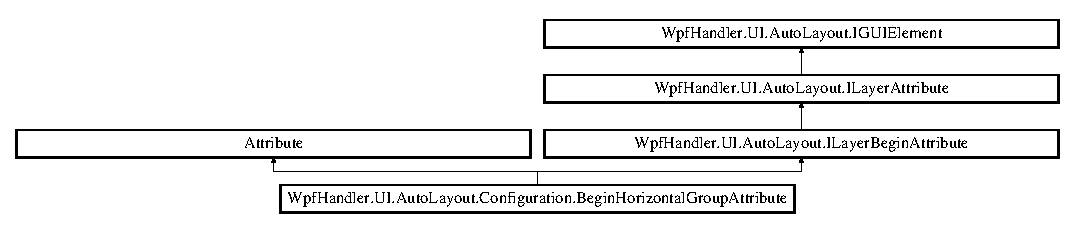
\includegraphics[height=2.635294cm]{db/d6f/class_wpf_handler_1_1_u_i_1_1_auto_layout_1_1_configuration_1_1_begin_horizontal_group_attribute}
\end{center}
\end{figure}
\subsection*{Public Member Functions}
\begin{DoxyCompactItemize}
\item 
void \mbox{\hyperlink{class_wpf_handler_1_1_u_i_1_1_auto_layout_1_1_configuration_1_1_begin_horizontal_group_attribute_a8bb61f969389bece86c87fbfa44d4c82}{On\+Layout}} (ref \mbox{\hyperlink{class_wpf_handler_1_1_u_i_1_1_auto_layout_1_1_layout_layer}{Layout\+Layer}} layer, params object\mbox{[}$\,$\mbox{]} args)
\begin{DoxyCompactList}\small\item\em Going one layer deeper into \mbox{\hyperlink{namespace_wpf_handler_1_1_u_i}{UI}} layout. All child element will be placed in horizontal order till calling of the End\+Group element. \end{DoxyCompactList}\end{DoxyCompactItemize}
\subsection*{Properties}
\begin{DoxyCompactItemize}
\item 
\mbox{\hyperlink{class_wpf_handler_1_1_u_i_1_1_auto_layout_1_1_layout_layer}{Layout\+Layer}} \mbox{\hyperlink{class_wpf_handler_1_1_u_i_1_1_auto_layout_1_1_configuration_1_1_begin_horizontal_group_attribute_afbdce9f3ac40b7f4bd6f2f675beafe36}{Layer}}\hspace{0.3cm}{\ttfamily  \mbox{[}get\mbox{]}}
\begin{DoxyCompactList}\small\item\em Layer that opereted into the handler. \end{DoxyCompactList}\end{DoxyCompactItemize}
\subsection*{Private Attributes}
\begin{DoxyCompactItemize}
\item 
\mbox{\hyperlink{class_wpf_handler_1_1_u_i_1_1_auto_layout_1_1_layout_layer}{Layout\+Layer}} \mbox{\hyperlink{class_wpf_handler_1_1_u_i_1_1_auto_layout_1_1_configuration_1_1_begin_horizontal_group_attribute_af50995071c008ef3fff87aa189a8256f}{\+\_\+\+Layer}}
\begin{DoxyCompactList}\small\item\em Bufer that contains layer. \end{DoxyCompactList}\end{DoxyCompactItemize}


\subsection{Detailed Description}
Starting a horizontal layout group. Will wait \mbox{\hyperlink{class_wpf_handler_1_1_u_i_1_1_auto_layout_1_1_configuration_1_1_end_group_attribute}{End\+Group\+Attribute}} to over the last begined group. 



\subsection{Member Function Documentation}
\mbox{\Hypertarget{class_wpf_handler_1_1_u_i_1_1_auto_layout_1_1_configuration_1_1_begin_horizontal_group_attribute_a8bb61f969389bece86c87fbfa44d4c82}\label{class_wpf_handler_1_1_u_i_1_1_auto_layout_1_1_configuration_1_1_begin_horizontal_group_attribute_a8bb61f969389bece86c87fbfa44d4c82}} 
\index{Wpf\+Handler\+::\+U\+I\+::\+Auto\+Layout\+::\+Configuration\+::\+Begin\+Horizontal\+Group\+Attribute@{Wpf\+Handler\+::\+U\+I\+::\+Auto\+Layout\+::\+Configuration\+::\+Begin\+Horizontal\+Group\+Attribute}!On\+Layout@{On\+Layout}}
\index{On\+Layout@{On\+Layout}!Wpf\+Handler\+::\+U\+I\+::\+Auto\+Layout\+::\+Configuration\+::\+Begin\+Horizontal\+Group\+Attribute@{Wpf\+Handler\+::\+U\+I\+::\+Auto\+Layout\+::\+Configuration\+::\+Begin\+Horizontal\+Group\+Attribute}}
\subsubsection{\texorpdfstring{On\+Layout()}{OnLayout()}}
{\footnotesize\ttfamily void Wpf\+Handler.\+U\+I.\+Auto\+Layout.\+Configuration.\+Begin\+Horizontal\+Group\+Attribute.\+On\+Layout (\begin{DoxyParamCaption}\item[{ref \mbox{\hyperlink{class_wpf_handler_1_1_u_i_1_1_auto_layout_1_1_layout_layer}{Layout\+Layer}}}]{layer,  }\item[{params object \mbox{[}$\,$\mbox{]}}]{args }\end{DoxyParamCaption})}



Going one layer deeper into \mbox{\hyperlink{namespace_wpf_handler_1_1_u_i}{UI}} layout. All child element will be placed in horizontal order till calling of the End\+Group element. 


\begin{DoxyParams}{Parameters}
{\em layer} & Curent layer. Refernece eill be changed to the new layer after performing.\\
\hline
{\em args} & Not using into that elelment.\\
\hline
\end{DoxyParams}


Implements \mbox{\hyperlink{interface_wpf_handler_1_1_u_i_1_1_auto_layout_1_1_i_g_u_i_element_a0ff16956f8e8187d51e1b36b6b9f894e}{Wpf\+Handler.\+U\+I.\+Auto\+Layout.\+I\+G\+U\+I\+Element}}.



\subsection{Member Data Documentation}
\mbox{\Hypertarget{class_wpf_handler_1_1_u_i_1_1_auto_layout_1_1_configuration_1_1_begin_horizontal_group_attribute_af50995071c008ef3fff87aa189a8256f}\label{class_wpf_handler_1_1_u_i_1_1_auto_layout_1_1_configuration_1_1_begin_horizontal_group_attribute_af50995071c008ef3fff87aa189a8256f}} 
\index{Wpf\+Handler\+::\+U\+I\+::\+Auto\+Layout\+::\+Configuration\+::\+Begin\+Horizontal\+Group\+Attribute@{Wpf\+Handler\+::\+U\+I\+::\+Auto\+Layout\+::\+Configuration\+::\+Begin\+Horizontal\+Group\+Attribute}!\+\_\+\+Layer@{\+\_\+\+Layer}}
\index{\+\_\+\+Layer@{\+\_\+\+Layer}!Wpf\+Handler\+::\+U\+I\+::\+Auto\+Layout\+::\+Configuration\+::\+Begin\+Horizontal\+Group\+Attribute@{Wpf\+Handler\+::\+U\+I\+::\+Auto\+Layout\+::\+Configuration\+::\+Begin\+Horizontal\+Group\+Attribute}}
\subsubsection{\texorpdfstring{\+\_\+\+Layer}{\_Layer}}
{\footnotesize\ttfamily \mbox{\hyperlink{class_wpf_handler_1_1_u_i_1_1_auto_layout_1_1_layout_layer}{Layout\+Layer}} Wpf\+Handler.\+U\+I.\+Auto\+Layout.\+Configuration.\+Begin\+Horizontal\+Group\+Attribute.\+\_\+\+Layer\hspace{0.3cm}{\ttfamily [private]}}



Bufer that contains layer. 



\subsection{Property Documentation}
\mbox{\Hypertarget{class_wpf_handler_1_1_u_i_1_1_auto_layout_1_1_configuration_1_1_begin_horizontal_group_attribute_afbdce9f3ac40b7f4bd6f2f675beafe36}\label{class_wpf_handler_1_1_u_i_1_1_auto_layout_1_1_configuration_1_1_begin_horizontal_group_attribute_afbdce9f3ac40b7f4bd6f2f675beafe36}} 
\index{Wpf\+Handler\+::\+U\+I\+::\+Auto\+Layout\+::\+Configuration\+::\+Begin\+Horizontal\+Group\+Attribute@{Wpf\+Handler\+::\+U\+I\+::\+Auto\+Layout\+::\+Configuration\+::\+Begin\+Horizontal\+Group\+Attribute}!Layer@{Layer}}
\index{Layer@{Layer}!Wpf\+Handler\+::\+U\+I\+::\+Auto\+Layout\+::\+Configuration\+::\+Begin\+Horizontal\+Group\+Attribute@{Wpf\+Handler\+::\+U\+I\+::\+Auto\+Layout\+::\+Configuration\+::\+Begin\+Horizontal\+Group\+Attribute}}
\subsubsection{\texorpdfstring{Layer}{Layer}}
{\footnotesize\ttfamily \mbox{\hyperlink{class_wpf_handler_1_1_u_i_1_1_auto_layout_1_1_layout_layer}{Layout\+Layer}} Wpf\+Handler.\+U\+I.\+Auto\+Layout.\+Configuration.\+Begin\+Horizontal\+Group\+Attribute.\+Layer\hspace{0.3cm}{\ttfamily [get]}}



Layer that opereted into the handler. 



The documentation for this class was generated from the following file\+:\begin{DoxyCompactItemize}
\item 
D\+:/\+Work/\+Git\+Hub/wpf-\/handler/\+Wpf\+Handler/\+U\+I/\+Auto\+Layout/\+Configuration/Begin\+Horizontal\+Group\+Attribute.\+cs\end{DoxyCompactItemize}

\hypertarget{class_wpf_handler_1_1_u_i_1_1_auto_layout_1_1_configuration_1_1_begin_vertical_group_attribute}{}\section{Wpf\+Handler.\+U\+I.\+Auto\+Layout.\+Configuration.\+Begin\+Vertical\+Group\+Attribute Class Reference}
\label{class_wpf_handler_1_1_u_i_1_1_auto_layout_1_1_configuration_1_1_begin_vertical_group_attribute}\index{Wpf\+Handler.\+U\+I.\+Auto\+Layout.\+Configuration.\+Begin\+Vertical\+Group\+Attribute@{Wpf\+Handler.\+U\+I.\+Auto\+Layout.\+Configuration.\+Begin\+Vertical\+Group\+Attribute}}


Starting vertical layout group. Will wait End\+Vertical to over the last begined group.  


Inheritance diagram for Wpf\+Handler.\+U\+I.\+Auto\+Layout.\+Configuration.\+Begin\+Vertical\+Group\+Attribute\+:\begin{figure}[H]
\begin{center}
\leavevmode
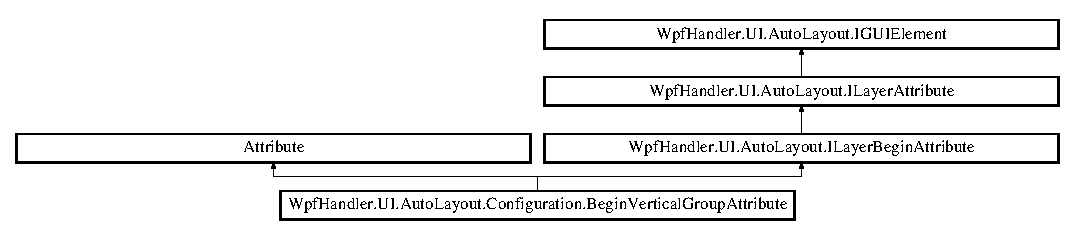
\includegraphics[height=2.718446cm]{de/db7/class_wpf_handler_1_1_u_i_1_1_auto_layout_1_1_configuration_1_1_begin_vertical_group_attribute}
\end{center}
\end{figure}
\subsection*{Public Member Functions}
\begin{DoxyCompactItemize}
\item 
void \mbox{\hyperlink{class_wpf_handler_1_1_u_i_1_1_auto_layout_1_1_configuration_1_1_begin_vertical_group_attribute_a52859bc4d83f107cbae35d20ae97ce83}{On\+Layout}} (ref \mbox{\hyperlink{class_wpf_handler_1_1_u_i_1_1_auto_layout_1_1_layout_layer}{Layout\+Layer}} layer, params object\mbox{[}$\,$\mbox{]} args)
\begin{DoxyCompactList}\small\item\em Going one layer deeper into \mbox{\hyperlink{namespace_wpf_handler_1_1_u_i}{UI}} layout. All child element will be placed in vertical order till calling of the End\+Group element. \end{DoxyCompactList}\end{DoxyCompactItemize}
\subsection*{Properties}
\begin{DoxyCompactItemize}
\item 
\mbox{\hyperlink{class_wpf_handler_1_1_u_i_1_1_auto_layout_1_1_layout_layer}{Layout\+Layer}} \mbox{\hyperlink{class_wpf_handler_1_1_u_i_1_1_auto_layout_1_1_configuration_1_1_begin_vertical_group_attribute_aba42e4648d684e4a0091d4157e58c19d}{Layer}}\hspace{0.3cm}{\ttfamily  \mbox{[}get\mbox{]}}
\begin{DoxyCompactList}\small\item\em Layer that opereted into the handler. \end{DoxyCompactList}\end{DoxyCompactItemize}
\subsection*{Private Attributes}
\begin{DoxyCompactItemize}
\item 
\mbox{\hyperlink{class_wpf_handler_1_1_u_i_1_1_auto_layout_1_1_layout_layer}{Layout\+Layer}} \mbox{\hyperlink{class_wpf_handler_1_1_u_i_1_1_auto_layout_1_1_configuration_1_1_begin_vertical_group_attribute_ac18db79463ee3229241875a881b71c48}{\+\_\+\+Layer}}
\begin{DoxyCompactList}\small\item\em Bufer that contains layer. \end{DoxyCompactList}\end{DoxyCompactItemize}


\subsection{Detailed Description}
Starting vertical layout group. Will wait End\+Vertical to over the last begined group. 



\subsection{Member Function Documentation}
\mbox{\Hypertarget{class_wpf_handler_1_1_u_i_1_1_auto_layout_1_1_configuration_1_1_begin_vertical_group_attribute_a52859bc4d83f107cbae35d20ae97ce83}\label{class_wpf_handler_1_1_u_i_1_1_auto_layout_1_1_configuration_1_1_begin_vertical_group_attribute_a52859bc4d83f107cbae35d20ae97ce83}} 
\index{Wpf\+Handler\+::\+U\+I\+::\+Auto\+Layout\+::\+Configuration\+::\+Begin\+Vertical\+Group\+Attribute@{Wpf\+Handler\+::\+U\+I\+::\+Auto\+Layout\+::\+Configuration\+::\+Begin\+Vertical\+Group\+Attribute}!On\+Layout@{On\+Layout}}
\index{On\+Layout@{On\+Layout}!Wpf\+Handler\+::\+U\+I\+::\+Auto\+Layout\+::\+Configuration\+::\+Begin\+Vertical\+Group\+Attribute@{Wpf\+Handler\+::\+U\+I\+::\+Auto\+Layout\+::\+Configuration\+::\+Begin\+Vertical\+Group\+Attribute}}
\subsubsection{\texorpdfstring{On\+Layout()}{OnLayout()}}
{\footnotesize\ttfamily void Wpf\+Handler.\+U\+I.\+Auto\+Layout.\+Configuration.\+Begin\+Vertical\+Group\+Attribute.\+On\+Layout (\begin{DoxyParamCaption}\item[{ref \mbox{\hyperlink{class_wpf_handler_1_1_u_i_1_1_auto_layout_1_1_layout_layer}{Layout\+Layer}}}]{layer,  }\item[{params object \mbox{[}$\,$\mbox{]}}]{args }\end{DoxyParamCaption})}



Going one layer deeper into \mbox{\hyperlink{namespace_wpf_handler_1_1_u_i}{UI}} layout. All child element will be placed in vertical order till calling of the End\+Group element. 


\begin{DoxyParams}{Parameters}
{\em layer} & Curent layer. Refernece eill be changed to the new layer after performing.\\
\hline
{\em args} & Not using into that elelment.\\
\hline
\end{DoxyParams}


Implements \mbox{\hyperlink{interface_wpf_handler_1_1_u_i_1_1_auto_layout_1_1_i_g_u_i_element_a0ff16956f8e8187d51e1b36b6b9f894e}{Wpf\+Handler.\+U\+I.\+Auto\+Layout.\+I\+G\+U\+I\+Element}}.



\subsection{Member Data Documentation}
\mbox{\Hypertarget{class_wpf_handler_1_1_u_i_1_1_auto_layout_1_1_configuration_1_1_begin_vertical_group_attribute_ac18db79463ee3229241875a881b71c48}\label{class_wpf_handler_1_1_u_i_1_1_auto_layout_1_1_configuration_1_1_begin_vertical_group_attribute_ac18db79463ee3229241875a881b71c48}} 
\index{Wpf\+Handler\+::\+U\+I\+::\+Auto\+Layout\+::\+Configuration\+::\+Begin\+Vertical\+Group\+Attribute@{Wpf\+Handler\+::\+U\+I\+::\+Auto\+Layout\+::\+Configuration\+::\+Begin\+Vertical\+Group\+Attribute}!\+\_\+\+Layer@{\+\_\+\+Layer}}
\index{\+\_\+\+Layer@{\+\_\+\+Layer}!Wpf\+Handler\+::\+U\+I\+::\+Auto\+Layout\+::\+Configuration\+::\+Begin\+Vertical\+Group\+Attribute@{Wpf\+Handler\+::\+U\+I\+::\+Auto\+Layout\+::\+Configuration\+::\+Begin\+Vertical\+Group\+Attribute}}
\subsubsection{\texorpdfstring{\+\_\+\+Layer}{\_Layer}}
{\footnotesize\ttfamily \mbox{\hyperlink{class_wpf_handler_1_1_u_i_1_1_auto_layout_1_1_layout_layer}{Layout\+Layer}} Wpf\+Handler.\+U\+I.\+Auto\+Layout.\+Configuration.\+Begin\+Vertical\+Group\+Attribute.\+\_\+\+Layer\hspace{0.3cm}{\ttfamily [private]}}



Bufer that contains layer. 



\subsection{Property Documentation}
\mbox{\Hypertarget{class_wpf_handler_1_1_u_i_1_1_auto_layout_1_1_configuration_1_1_begin_vertical_group_attribute_aba42e4648d684e4a0091d4157e58c19d}\label{class_wpf_handler_1_1_u_i_1_1_auto_layout_1_1_configuration_1_1_begin_vertical_group_attribute_aba42e4648d684e4a0091d4157e58c19d}} 
\index{Wpf\+Handler\+::\+U\+I\+::\+Auto\+Layout\+::\+Configuration\+::\+Begin\+Vertical\+Group\+Attribute@{Wpf\+Handler\+::\+U\+I\+::\+Auto\+Layout\+::\+Configuration\+::\+Begin\+Vertical\+Group\+Attribute}!Layer@{Layer}}
\index{Layer@{Layer}!Wpf\+Handler\+::\+U\+I\+::\+Auto\+Layout\+::\+Configuration\+::\+Begin\+Vertical\+Group\+Attribute@{Wpf\+Handler\+::\+U\+I\+::\+Auto\+Layout\+::\+Configuration\+::\+Begin\+Vertical\+Group\+Attribute}}
\subsubsection{\texorpdfstring{Layer}{Layer}}
{\footnotesize\ttfamily \mbox{\hyperlink{class_wpf_handler_1_1_u_i_1_1_auto_layout_1_1_layout_layer}{Layout\+Layer}} Wpf\+Handler.\+U\+I.\+Auto\+Layout.\+Configuration.\+Begin\+Vertical\+Group\+Attribute.\+Layer\hspace{0.3cm}{\ttfamily [get]}}



Layer that opereted into the handler. 



The documentation for this class was generated from the following file\+:\begin{DoxyCompactItemize}
\item 
D\+:/\+Work/\+Git\+Hub/wpf-\/handler/\+Wpf\+Handler/\+U\+I/\+Auto\+Layout/\+Configuration/Begin\+Vertical\+Group\+Attribute.\+cs\end{DoxyCompactItemize}

\hypertarget{class_wpf_handler_1_1_u_i_1_1_effects_1_1_blur_effect}{}\section{Wpf\+Handler.\+U\+I.\+Effects.\+Blur\+Effect Class Reference}
\label{class_wpf_handler_1_1_u_i_1_1_effects_1_1_blur_effect}\index{Wpf\+Handler.\+U\+I.\+Effects.\+Blur\+Effect@{Wpf\+Handler.\+U\+I.\+Effects.\+Blur\+Effect}}


Provide blur operations.  


\subsection*{Static Public Member Functions}
\begin{DoxyCompactItemize}
\item 
static Double\+Animation \mbox{\hyperlink{class_wpf_handler_1_1_u_i_1_1_effects_1_1_blur_effect_a4f7eaa622e8bc4226f865a7f9afa5d07}{Blur\+Apply}} (U\+I\+Element element, double blur\+Radius, Time\+Span duration, Time\+Span begin\+Time, Fill\+Behavior fill\+Behavior)
\begin{DoxyCompactList}\small\item\em Turning blur on. \end{DoxyCompactList}\item 
static Double\+Animation \mbox{\hyperlink{class_wpf_handler_1_1_u_i_1_1_effects_1_1_blur_effect_ac4161005a77de53909ed18c82477491a}{Blur\+Apply}} (U\+I\+Element element, double blur\+Radius, Time\+Span duration, Time\+Span begin\+Time, Fill\+Behavior fill\+Behavior, Action$<$ Double\+Animation $>$ init\+Handler)
\begin{DoxyCompactList}\small\item\em Turning blur on. \end{DoxyCompactList}\item 
static Double\+Animation \mbox{\hyperlink{class_wpf_handler_1_1_u_i_1_1_effects_1_1_blur_effect_a1d0e1aab31423c3bac492e41c51554b5}{Blur\+Disable}} (U\+I\+Element element, Time\+Span duration, Time\+Span begin\+Time)
\begin{DoxyCompactList}\small\item\em Turning blur off. \end{DoxyCompactList}\item 
static Double\+Animation \mbox{\hyperlink{class_wpf_handler_1_1_u_i_1_1_effects_1_1_blur_effect_a894c9100c3d72af41a15ab60ac4a62c1}{Blur\+Disable}} (U\+I\+Element element, Time\+Span duration, Time\+Span begin\+Time, Action$<$ Double\+Animation $>$ init\+Handler)
\begin{DoxyCompactList}\small\item\em Turning blur off. \end{DoxyCompactList}\end{DoxyCompactItemize}


\subsection{Detailed Description}
Provide blur operations. 



\subsection{Member Function Documentation}
\mbox{\Hypertarget{class_wpf_handler_1_1_u_i_1_1_effects_1_1_blur_effect_a4f7eaa622e8bc4226f865a7f9afa5d07}\label{class_wpf_handler_1_1_u_i_1_1_effects_1_1_blur_effect_a4f7eaa622e8bc4226f865a7f9afa5d07}} 
\index{Wpf\+Handler\+::\+U\+I\+::\+Effects\+::\+Blur\+Effect@{Wpf\+Handler\+::\+U\+I\+::\+Effects\+::\+Blur\+Effect}!Blur\+Apply@{Blur\+Apply}}
\index{Blur\+Apply@{Blur\+Apply}!Wpf\+Handler\+::\+U\+I\+::\+Effects\+::\+Blur\+Effect@{Wpf\+Handler\+::\+U\+I\+::\+Effects\+::\+Blur\+Effect}}
\subsubsection{\texorpdfstring{Blur\+Apply()}{BlurApply()}\hspace{0.1cm}{\footnotesize\ttfamily [1/2]}}
{\footnotesize\ttfamily static Double\+Animation Wpf\+Handler.\+U\+I.\+Effects.\+Blur\+Effect.\+Blur\+Apply (\begin{DoxyParamCaption}\item[{U\+I\+Element}]{element,  }\item[{double}]{blur\+Radius,  }\item[{Time\+Span}]{duration,  }\item[{Time\+Span}]{begin\+Time,  }\item[{Fill\+Behavior}]{fill\+Behavior }\end{DoxyParamCaption})\hspace{0.3cm}{\ttfamily [static]}}



Turning blur on. 


\begin{DoxyParams}{Parameters}
{\em element} & bluring element\\
\hline
{\em blur\+Radius} & blur radius\\
\hline
{\em duration} & blur animation duration\\
\hline
{\em begin\+Time} & blur animation delay\\
\hline
{\em fill\+Behavior} & Specifies how a System.\+Windows.\+Media.\+Animation.\+Timeline behaves when it is outside its active period but its parent is inside its active or hold period.\\
\hline
\end{DoxyParams}
\begin{DoxyReturn}{Returns}
Created animation.
\end{DoxyReturn}
\mbox{\Hypertarget{class_wpf_handler_1_1_u_i_1_1_effects_1_1_blur_effect_ac4161005a77de53909ed18c82477491a}\label{class_wpf_handler_1_1_u_i_1_1_effects_1_1_blur_effect_ac4161005a77de53909ed18c82477491a}} 
\index{Wpf\+Handler\+::\+U\+I\+::\+Effects\+::\+Blur\+Effect@{Wpf\+Handler\+::\+U\+I\+::\+Effects\+::\+Blur\+Effect}!Blur\+Apply@{Blur\+Apply}}
\index{Blur\+Apply@{Blur\+Apply}!Wpf\+Handler\+::\+U\+I\+::\+Effects\+::\+Blur\+Effect@{Wpf\+Handler\+::\+U\+I\+::\+Effects\+::\+Blur\+Effect}}
\subsubsection{\texorpdfstring{Blur\+Apply()}{BlurApply()}\hspace{0.1cm}{\footnotesize\ttfamily [2/2]}}
{\footnotesize\ttfamily static Double\+Animation Wpf\+Handler.\+U\+I.\+Effects.\+Blur\+Effect.\+Blur\+Apply (\begin{DoxyParamCaption}\item[{U\+I\+Element}]{element,  }\item[{double}]{blur\+Radius,  }\item[{Time\+Span}]{duration,  }\item[{Time\+Span}]{begin\+Time,  }\item[{Fill\+Behavior}]{fill\+Behavior,  }\item[{Action$<$ Double\+Animation $>$}]{init\+Handler }\end{DoxyParamCaption})\hspace{0.3cm}{\ttfamily [static]}}



Turning blur on. 


\begin{DoxyParams}{Parameters}
{\em element} & bluring element\\
\hline
{\em blur\+Radius} & blur radius\\
\hline
{\em duration} & blur animation duration\\
\hline
{\em begin\+Time} & blur animation delay\\
\hline
{\em fill\+Behavior} & Specifies how a System.\+Windows.\+Media.\+Animation.\+Timeline behaves when it is outside its active period but its parent is inside its active or hold period.\\
\hline
{\em init\+Handler} & Handler that would be called before animation start. There you can subscrube on events or reconfigurate settigns.\\
\hline
\end{DoxyParams}
\begin{DoxyReturn}{Returns}
Created animation.
\end{DoxyReturn}
\mbox{\Hypertarget{class_wpf_handler_1_1_u_i_1_1_effects_1_1_blur_effect_a1d0e1aab31423c3bac492e41c51554b5}\label{class_wpf_handler_1_1_u_i_1_1_effects_1_1_blur_effect_a1d0e1aab31423c3bac492e41c51554b5}} 
\index{Wpf\+Handler\+::\+U\+I\+::\+Effects\+::\+Blur\+Effect@{Wpf\+Handler\+::\+U\+I\+::\+Effects\+::\+Blur\+Effect}!Blur\+Disable@{Blur\+Disable}}
\index{Blur\+Disable@{Blur\+Disable}!Wpf\+Handler\+::\+U\+I\+::\+Effects\+::\+Blur\+Effect@{Wpf\+Handler\+::\+U\+I\+::\+Effects\+::\+Blur\+Effect}}
\subsubsection{\texorpdfstring{Blur\+Disable()}{BlurDisable()}\hspace{0.1cm}{\footnotesize\ttfamily [1/2]}}
{\footnotesize\ttfamily static Double\+Animation Wpf\+Handler.\+U\+I.\+Effects.\+Blur\+Effect.\+Blur\+Disable (\begin{DoxyParamCaption}\item[{U\+I\+Element}]{element,  }\item[{Time\+Span}]{duration,  }\item[{Time\+Span}]{begin\+Time }\end{DoxyParamCaption})\hspace{0.3cm}{\ttfamily [static]}}



Turning blur off. 


\begin{DoxyParams}{Parameters}
{\em element} & bluring element\\
\hline
{\em duration} & blur animation duration\\
\hline
{\em begin\+Time} & blur animation delay\\
\hline
\end{DoxyParams}
\begin{DoxyReturn}{Returns}
Created animation.
\end{DoxyReturn}
\mbox{\Hypertarget{class_wpf_handler_1_1_u_i_1_1_effects_1_1_blur_effect_a894c9100c3d72af41a15ab60ac4a62c1}\label{class_wpf_handler_1_1_u_i_1_1_effects_1_1_blur_effect_a894c9100c3d72af41a15ab60ac4a62c1}} 
\index{Wpf\+Handler\+::\+U\+I\+::\+Effects\+::\+Blur\+Effect@{Wpf\+Handler\+::\+U\+I\+::\+Effects\+::\+Blur\+Effect}!Blur\+Disable@{Blur\+Disable}}
\index{Blur\+Disable@{Blur\+Disable}!Wpf\+Handler\+::\+U\+I\+::\+Effects\+::\+Blur\+Effect@{Wpf\+Handler\+::\+U\+I\+::\+Effects\+::\+Blur\+Effect}}
\subsubsection{\texorpdfstring{Blur\+Disable()}{BlurDisable()}\hspace{0.1cm}{\footnotesize\ttfamily [2/2]}}
{\footnotesize\ttfamily static Double\+Animation Wpf\+Handler.\+U\+I.\+Effects.\+Blur\+Effect.\+Blur\+Disable (\begin{DoxyParamCaption}\item[{U\+I\+Element}]{element,  }\item[{Time\+Span}]{duration,  }\item[{Time\+Span}]{begin\+Time,  }\item[{Action$<$ Double\+Animation $>$}]{init\+Handler }\end{DoxyParamCaption})\hspace{0.3cm}{\ttfamily [static]}}



Turning blur off. 


\begin{DoxyParams}{Parameters}
{\em element} & bluring element\\
\hline
{\em duration} & blur animation duration\\
\hline
{\em begin\+Time} & blur animation delay\\
\hline
{\em init\+Handler} & Handler that would be called before animation start. There you can subscrube on events or reconfigurate settigns.\\
\hline
\end{DoxyParams}
\begin{DoxyReturn}{Returns}
Created animation.
\end{DoxyReturn}


The documentation for this class was generated from the following file\+:\begin{DoxyCompactItemize}
\item 
D\+:/\+Work/\+Git\+Hub/wpf-\/handler/\+Wpf\+Handler/\+U\+I/\+Effects/Blur\+Effect.\+cs\end{DoxyCompactItemize}

\hypertarget{class_wpf_handler_1_1_u_i_1_1_controls_1_1_catalog_button}{}\section{Wpf\+Handler.\+U\+I.\+Controls.\+Catalog\+Button Class Reference}
\label{class_wpf_handler_1_1_u_i_1_1_controls_1_1_catalog_button}\index{Wpf\+Handler.\+U\+I.\+Controls.\+Catalog\+Button@{Wpf\+Handler.\+U\+I.\+Controls.\+Catalog\+Button}}


\mbox{\hyperlink{class_wpf_handler_1_1_u_i_1_1_controls_1_1_catalog_button}{Catalog\+Button}}  


Inheritance diagram for Wpf\+Handler.\+U\+I.\+Controls.\+Catalog\+Button\+:\begin{figure}[H]
\begin{center}
\leavevmode
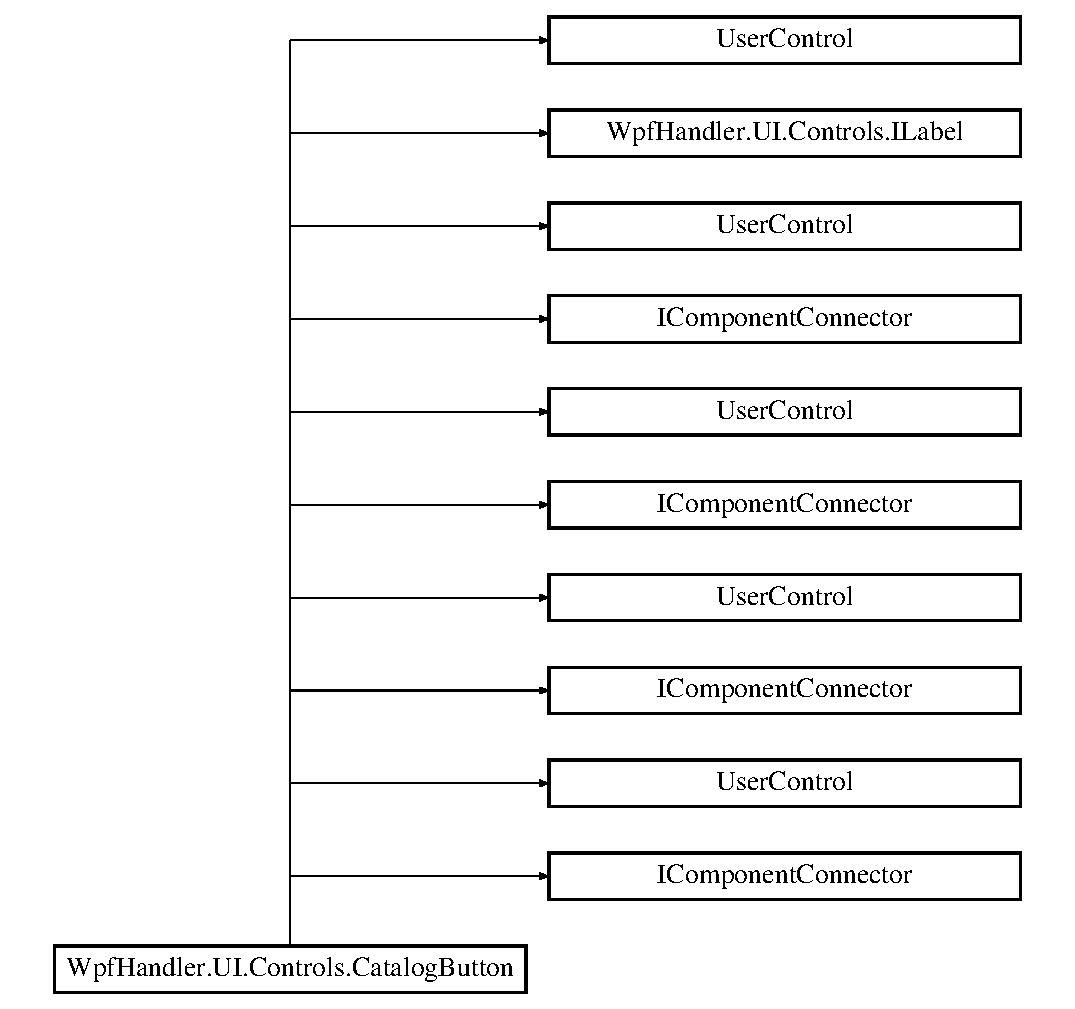
\includegraphics[height=11.000000cm]{d0/d24/class_wpf_handler_1_1_u_i_1_1_controls_1_1_catalog_button}
\end{center}
\end{figure}
\subsection*{Public Member Functions}
\begin{DoxyCompactItemize}
\item 
void \mbox{\hyperlink{class_wpf_handler_1_1_u_i_1_1_controls_1_1_catalog_button_abd3ec610152200149f7ac8a4f3d63594}{Initialize\+Component}} ()
\begin{DoxyCompactList}\small\item\em Initialize\+Component \end{DoxyCompactList}\item 
void \mbox{\hyperlink{class_wpf_handler_1_1_u_i_1_1_controls_1_1_catalog_button_abd3ec610152200149f7ac8a4f3d63594}{Initialize\+Component}} ()
\begin{DoxyCompactList}\small\item\em Initialize\+Component \end{DoxyCompactList}\item 
void \mbox{\hyperlink{class_wpf_handler_1_1_u_i_1_1_controls_1_1_catalog_button_abd3ec610152200149f7ac8a4f3d63594}{Initialize\+Component}} ()
\begin{DoxyCompactList}\small\item\em Initialize\+Component \end{DoxyCompactList}\item 
void \mbox{\hyperlink{class_wpf_handler_1_1_u_i_1_1_controls_1_1_catalog_button_abd3ec610152200149f7ac8a4f3d63594}{Initialize\+Component}} ()
\begin{DoxyCompactList}\small\item\em Initialize\+Component \end{DoxyCompactList}\item 
\mbox{\hyperlink{class_wpf_handler_1_1_u_i_1_1_controls_1_1_catalog_button_a448a9b9dc299b55303d67f4e4b13c2d7}{Catalog\+Button}} ()
\begin{DoxyCompactList}\small\item\em Initialisign the catalog button. \end{DoxyCompactList}\end{DoxyCompactItemize}
\subsection*{Static Public Attributes}
\begin{DoxyCompactItemize}
\item 
static readonly Dependency\+Property \mbox{\hyperlink{class_wpf_handler_1_1_u_i_1_1_controls_1_1_catalog_button_ab4d5e54d4e9edb3c3c34849f3ce9dce4}{Label\+Property}}
\begin{DoxyCompactList}\small\item\em Bridging X\+A\+ML declaring and the member. \end{DoxyCompactList}\item 
static readonly Dependency\+Property \mbox{\hyperlink{class_wpf_handler_1_1_u_i_1_1_controls_1_1_catalog_button_a607704571d71a9ca79f824962e860f3d}{Unfocused\+Background\+Color\+Property}}
\begin{DoxyCompactList}\small\item\em Bridging X\+A\+ML declaring and the member. \end{DoxyCompactList}\item 
static readonly Dependency\+Property \mbox{\hyperlink{class_wpf_handler_1_1_u_i_1_1_controls_1_1_catalog_button_afce5107ac54bea54129ff8386d9d35e8}{Focused\+Background\+Color\+Property}}
\begin{DoxyCompactList}\small\item\em Bridging X\+A\+ML declaring and the member. \end{DoxyCompactList}\item 
static readonly Dependency\+Property \mbox{\hyperlink{class_wpf_handler_1_1_u_i_1_1_controls_1_1_catalog_button_aa6d95a94eb81ade4a15936e88d9344d7}{Text\+Color\+Property}}
\begin{DoxyCompactList}\small\item\em Bridging X\+A\+ML declaring and the member. \end{DoxyCompactList}\item 
static readonly Dependency\+Property \mbox{\hyperlink{class_wpf_handler_1_1_u_i_1_1_controls_1_1_catalog_button_ab35a69a899697dca0a651d21ce61ebea}{Click\+Callback\+Property}}
\begin{DoxyCompactList}\small\item\em Bridging X\+A\+ML declaring and the member. \end{DoxyCompactList}\end{DoxyCompactItemize}
\subsection*{Package Attributes}
\begin{DoxyCompactItemize}
\item 
\mbox{\Hypertarget{class_wpf_handler_1_1_u_i_1_1_controls_1_1_catalog_button_a904217841fac9694a0496fca2e43419c}\label{class_wpf_handler_1_1_u_i_1_1_controls_1_1_catalog_button_a904217841fac9694a0496fca2e43419c}} 
System.\+Windows.\+Controls.\+Button {\bfseries catalog\+Button}
\end{DoxyCompactItemize}
\subsection*{Properties}
\begin{DoxyCompactItemize}
\item 
string \mbox{\hyperlink{class_wpf_handler_1_1_u_i_1_1_controls_1_1_catalog_button_ae34f49ccfd0f7a78d44a0a0beed99ed8}{Label}}\hspace{0.3cm}{\ttfamily  \mbox{[}get, set\mbox{]}}
\begin{DoxyCompactList}\small\item\em Text that will be displayed on the button. \end{DoxyCompactList}\item 
int \mbox{\hyperlink{class_wpf_handler_1_1_u_i_1_1_controls_1_1_catalog_button_abf5864543b3338cad73968a464586543}{Hierarchy\+Level}} = 1\hspace{0.3cm}{\ttfamily  \mbox{[}get, set\mbox{]}}
\begin{DoxyCompactList}\small\item\em Define offset of the button text. \end{DoxyCompactList}\item 
Thickness \mbox{\hyperlink{class_wpf_handler_1_1_u_i_1_1_controls_1_1_catalog_button_ab427b14cc2815b6d085f5c159cd0bb21}{Auto\+Margin}}\hspace{0.3cm}{\ttfamily  \mbox{[}get\mbox{]}}
\begin{DoxyCompactList}\small\item\em Compute margine relative to hierarchy level. \end{DoxyCompactList}\item 
Brush \mbox{\hyperlink{class_wpf_handler_1_1_u_i_1_1_controls_1_1_catalog_button_a75b1005b0624dd175bc8403be01ad71f}{Unfocused\+Background\+Color}}\hspace{0.3cm}{\ttfamily  \mbox{[}get, set\mbox{]}}
\begin{DoxyCompactList}\small\item\em Collor of button when it unfocused. \end{DoxyCompactList}\item 
Brush \mbox{\hyperlink{class_wpf_handler_1_1_u_i_1_1_controls_1_1_catalog_button_acd3112c31263741ec183d439e55242a6}{Focused\+Background\+Color}}\hspace{0.3cm}{\ttfamily  \mbox{[}get, set\mbox{]}}
\begin{DoxyCompactList}\small\item\em Color of button when it focused. \end{DoxyCompactList}\item 
Brush \mbox{\hyperlink{class_wpf_handler_1_1_u_i_1_1_controls_1_1_catalog_button_a1362ded51e8334d84f7daf89e9f656ce}{Text\+Color}}\hspace{0.3cm}{\ttfamily  \mbox{[}get, set\mbox{]}}
\begin{DoxyCompactList}\small\item\em Collor of the text. \end{DoxyCompactList}\item 
Action$<$ object $>$ \mbox{\hyperlink{class_wpf_handler_1_1_u_i_1_1_controls_1_1_catalog_button_a06e2c59dcf54d8094d2b84fa6a558c56}{Click\+Callback}}\hspace{0.3cm}{\ttfamily  \mbox{[}get, set\mbox{]}}
\begin{DoxyCompactList}\small\item\em Method that will has been calling during click on button. \end{DoxyCompactList}\item 
float \mbox{\hyperlink{class_wpf_handler_1_1_u_i_1_1_controls_1_1_catalog_button_ad02761d35dd16eacc261a9bcfd518e88}{Label\+Width}}\hspace{0.3cm}{\ttfamily  \mbox{[}get, set\mbox{]}}
\begin{DoxyCompactList}\small\item\em Not supported. \end{DoxyCompactList}\end{DoxyCompactItemize}
\subsection*{Private Member Functions}
\begin{DoxyCompactItemize}
\item 
\mbox{\Hypertarget{class_wpf_handler_1_1_u_i_1_1_controls_1_1_catalog_button_a8b8d46e0277bc37fa5b44878ff08227d}\label{class_wpf_handler_1_1_u_i_1_1_controls_1_1_catalog_button_a8b8d46e0277bc37fa5b44878ff08227d}} 
void System.\+Windows.\+Markup.\+I\+Component\+Connector. {\bfseries Connect} (int connection\+Id, object target)
\item 
\mbox{\Hypertarget{class_wpf_handler_1_1_u_i_1_1_controls_1_1_catalog_button_a8b8d46e0277bc37fa5b44878ff08227d}\label{class_wpf_handler_1_1_u_i_1_1_controls_1_1_catalog_button_a8b8d46e0277bc37fa5b44878ff08227d}} 
void System.\+Windows.\+Markup.\+I\+Component\+Connector. {\bfseries Connect} (int connection\+Id, object target)
\item 
\mbox{\Hypertarget{class_wpf_handler_1_1_u_i_1_1_controls_1_1_catalog_button_a8b8d46e0277bc37fa5b44878ff08227d}\label{class_wpf_handler_1_1_u_i_1_1_controls_1_1_catalog_button_a8b8d46e0277bc37fa5b44878ff08227d}} 
void System.\+Windows.\+Markup.\+I\+Component\+Connector. {\bfseries Connect} (int connection\+Id, object target)
\item 
\mbox{\Hypertarget{class_wpf_handler_1_1_u_i_1_1_controls_1_1_catalog_button_a8b8d46e0277bc37fa5b44878ff08227d}\label{class_wpf_handler_1_1_u_i_1_1_controls_1_1_catalog_button_a8b8d46e0277bc37fa5b44878ff08227d}} 
void System.\+Windows.\+Markup.\+I\+Component\+Connector. {\bfseries Connect} (int connection\+Id, object target)
\item 
void \mbox{\hyperlink{class_wpf_handler_1_1_u_i_1_1_controls_1_1_catalog_button_af586051be4f757942d42f6b3825a9aa0}{Catalog\+Button\+\_\+\+Click}} (object sender, Routed\+Event\+Args e)
\begin{DoxyCompactList}\small\item\em Callback that will has been calling when button will be clicked. \end{DoxyCompactList}\end{DoxyCompactItemize}
\subsection*{Private Attributes}
\begin{DoxyCompactItemize}
\item 
\mbox{\Hypertarget{class_wpf_handler_1_1_u_i_1_1_controls_1_1_catalog_button_ae16854f2ac8f8bccd5b7e9566815ab54}\label{class_wpf_handler_1_1_u_i_1_1_controls_1_1_catalog_button_ae16854f2ac8f8bccd5b7e9566815ab54}} 
bool {\bfseries \+\_\+content\+Loaded}
\end{DoxyCompactItemize}


\subsection{Detailed Description}
\mbox{\hyperlink{class_wpf_handler_1_1_u_i_1_1_controls_1_1_catalog_button}{Catalog\+Button}} 

Interaction logic for Catalog\+Button.\+xaml 

\subsection{Constructor \& Destructor Documentation}
\mbox{\Hypertarget{class_wpf_handler_1_1_u_i_1_1_controls_1_1_catalog_button_a448a9b9dc299b55303d67f4e4b13c2d7}\label{class_wpf_handler_1_1_u_i_1_1_controls_1_1_catalog_button_a448a9b9dc299b55303d67f4e4b13c2d7}} 
\index{Wpf\+Handler\+::\+U\+I\+::\+Controls\+::\+Catalog\+Button@{Wpf\+Handler\+::\+U\+I\+::\+Controls\+::\+Catalog\+Button}!Catalog\+Button@{Catalog\+Button}}
\index{Catalog\+Button@{Catalog\+Button}!Wpf\+Handler\+::\+U\+I\+::\+Controls\+::\+Catalog\+Button@{Wpf\+Handler\+::\+U\+I\+::\+Controls\+::\+Catalog\+Button}}
\subsubsection{\texorpdfstring{Catalog\+Button()}{CatalogButton()}}
{\footnotesize\ttfamily Wpf\+Handler.\+U\+I.\+Controls.\+Catalog\+Button.\+Catalog\+Button (\begin{DoxyParamCaption}{ }\end{DoxyParamCaption})}



Initialisign the catalog button. 

Trying to find \char`\"{}\+Menu\+Button\char`\"{} resource as Style. Applying in case if found. 

\subsection{Member Function Documentation}
\mbox{\Hypertarget{class_wpf_handler_1_1_u_i_1_1_controls_1_1_catalog_button_af586051be4f757942d42f6b3825a9aa0}\label{class_wpf_handler_1_1_u_i_1_1_controls_1_1_catalog_button_af586051be4f757942d42f6b3825a9aa0}} 
\index{Wpf\+Handler\+::\+U\+I\+::\+Controls\+::\+Catalog\+Button@{Wpf\+Handler\+::\+U\+I\+::\+Controls\+::\+Catalog\+Button}!Catalog\+Button\+\_\+\+Click@{Catalog\+Button\+\_\+\+Click}}
\index{Catalog\+Button\+\_\+\+Click@{Catalog\+Button\+\_\+\+Click}!Wpf\+Handler\+::\+U\+I\+::\+Controls\+::\+Catalog\+Button@{Wpf\+Handler\+::\+U\+I\+::\+Controls\+::\+Catalog\+Button}}
\subsubsection{\texorpdfstring{Catalog\+Button\+\_\+\+Click()}{CatalogButton\_Click()}}
{\footnotesize\ttfamily void Wpf\+Handler.\+U\+I.\+Controls.\+Catalog\+Button.\+Catalog\+Button\+\_\+\+Click (\begin{DoxyParamCaption}\item[{object}]{sender,  }\item[{Routed\+Event\+Args}]{e }\end{DoxyParamCaption})\hspace{0.3cm}{\ttfamily [private]}}



Callback that will has been calling when button will be clicked. 


\begin{DoxyParams}{Parameters}
{\em sender} & \\
\hline
{\em e} & \\
\hline
\end{DoxyParams}
\mbox{\Hypertarget{class_wpf_handler_1_1_u_i_1_1_controls_1_1_catalog_button_abd3ec610152200149f7ac8a4f3d63594}\label{class_wpf_handler_1_1_u_i_1_1_controls_1_1_catalog_button_abd3ec610152200149f7ac8a4f3d63594}} 
\index{Wpf\+Handler\+::\+U\+I\+::\+Controls\+::\+Catalog\+Button@{Wpf\+Handler\+::\+U\+I\+::\+Controls\+::\+Catalog\+Button}!Initialize\+Component@{Initialize\+Component}}
\index{Initialize\+Component@{Initialize\+Component}!Wpf\+Handler\+::\+U\+I\+::\+Controls\+::\+Catalog\+Button@{Wpf\+Handler\+::\+U\+I\+::\+Controls\+::\+Catalog\+Button}}
\subsubsection{\texorpdfstring{Initialize\+Component()}{InitializeComponent()}\hspace{0.1cm}{\footnotesize\ttfamily [1/4]}}
{\footnotesize\ttfamily void Wpf\+Handler.\+U\+I.\+Controls.\+Catalog\+Button.\+Initialize\+Component (\begin{DoxyParamCaption}{ }\end{DoxyParamCaption})}



Initialize\+Component 

\mbox{\Hypertarget{class_wpf_handler_1_1_u_i_1_1_controls_1_1_catalog_button_abd3ec610152200149f7ac8a4f3d63594}\label{class_wpf_handler_1_1_u_i_1_1_controls_1_1_catalog_button_abd3ec610152200149f7ac8a4f3d63594}} 
\index{Wpf\+Handler\+::\+U\+I\+::\+Controls\+::\+Catalog\+Button@{Wpf\+Handler\+::\+U\+I\+::\+Controls\+::\+Catalog\+Button}!Initialize\+Component@{Initialize\+Component}}
\index{Initialize\+Component@{Initialize\+Component}!Wpf\+Handler\+::\+U\+I\+::\+Controls\+::\+Catalog\+Button@{Wpf\+Handler\+::\+U\+I\+::\+Controls\+::\+Catalog\+Button}}
\subsubsection{\texorpdfstring{Initialize\+Component()}{InitializeComponent()}\hspace{0.1cm}{\footnotesize\ttfamily [2/4]}}
{\footnotesize\ttfamily void Wpf\+Handler.\+U\+I.\+Controls.\+Catalog\+Button.\+Initialize\+Component (\begin{DoxyParamCaption}{ }\end{DoxyParamCaption})}



Initialize\+Component 

\mbox{\Hypertarget{class_wpf_handler_1_1_u_i_1_1_controls_1_1_catalog_button_abd3ec610152200149f7ac8a4f3d63594}\label{class_wpf_handler_1_1_u_i_1_1_controls_1_1_catalog_button_abd3ec610152200149f7ac8a4f3d63594}} 
\index{Wpf\+Handler\+::\+U\+I\+::\+Controls\+::\+Catalog\+Button@{Wpf\+Handler\+::\+U\+I\+::\+Controls\+::\+Catalog\+Button}!Initialize\+Component@{Initialize\+Component}}
\index{Initialize\+Component@{Initialize\+Component}!Wpf\+Handler\+::\+U\+I\+::\+Controls\+::\+Catalog\+Button@{Wpf\+Handler\+::\+U\+I\+::\+Controls\+::\+Catalog\+Button}}
\subsubsection{\texorpdfstring{Initialize\+Component()}{InitializeComponent()}\hspace{0.1cm}{\footnotesize\ttfamily [3/4]}}
{\footnotesize\ttfamily void Wpf\+Handler.\+U\+I.\+Controls.\+Catalog\+Button.\+Initialize\+Component (\begin{DoxyParamCaption}{ }\end{DoxyParamCaption})}



Initialize\+Component 

\mbox{\Hypertarget{class_wpf_handler_1_1_u_i_1_1_controls_1_1_catalog_button_abd3ec610152200149f7ac8a4f3d63594}\label{class_wpf_handler_1_1_u_i_1_1_controls_1_1_catalog_button_abd3ec610152200149f7ac8a4f3d63594}} 
\index{Wpf\+Handler\+::\+U\+I\+::\+Controls\+::\+Catalog\+Button@{Wpf\+Handler\+::\+U\+I\+::\+Controls\+::\+Catalog\+Button}!Initialize\+Component@{Initialize\+Component}}
\index{Initialize\+Component@{Initialize\+Component}!Wpf\+Handler\+::\+U\+I\+::\+Controls\+::\+Catalog\+Button@{Wpf\+Handler\+::\+U\+I\+::\+Controls\+::\+Catalog\+Button}}
\subsubsection{\texorpdfstring{Initialize\+Component()}{InitializeComponent()}\hspace{0.1cm}{\footnotesize\ttfamily [4/4]}}
{\footnotesize\ttfamily void Wpf\+Handler.\+U\+I.\+Controls.\+Catalog\+Button.\+Initialize\+Component (\begin{DoxyParamCaption}{ }\end{DoxyParamCaption})}



Initialize\+Component 



\subsection{Member Data Documentation}
\mbox{\Hypertarget{class_wpf_handler_1_1_u_i_1_1_controls_1_1_catalog_button_ab35a69a899697dca0a651d21ce61ebea}\label{class_wpf_handler_1_1_u_i_1_1_controls_1_1_catalog_button_ab35a69a899697dca0a651d21ce61ebea}} 
\index{Wpf\+Handler\+::\+U\+I\+::\+Controls\+::\+Catalog\+Button@{Wpf\+Handler\+::\+U\+I\+::\+Controls\+::\+Catalog\+Button}!Click\+Callback\+Property@{Click\+Callback\+Property}}
\index{Click\+Callback\+Property@{Click\+Callback\+Property}!Wpf\+Handler\+::\+U\+I\+::\+Controls\+::\+Catalog\+Button@{Wpf\+Handler\+::\+U\+I\+::\+Controls\+::\+Catalog\+Button}}
\subsubsection{\texorpdfstring{Click\+Callback\+Property}{ClickCallbackProperty}}
{\footnotesize\ttfamily readonly Dependency\+Property Wpf\+Handler.\+U\+I.\+Controls.\+Catalog\+Button.\+Click\+Callback\+Property\hspace{0.3cm}{\ttfamily [static]}}

{\bfseries Initial value\+:}
\begin{DoxyCode}
= DependencyProperty.Register(
          \textcolor{stringliteral}{"ClickCallback"}, typeof(Action<object>), typeof(\mbox{\hyperlink{class_wpf_handler_1_1_u_i_1_1_controls_1_1_catalog_button_a448a9b9dc299b55303d67f4e4b13c2d7}{CatalogButton}}))
\end{DoxyCode}


Bridging X\+A\+ML declaring and the member. 

\mbox{\Hypertarget{class_wpf_handler_1_1_u_i_1_1_controls_1_1_catalog_button_afce5107ac54bea54129ff8386d9d35e8}\label{class_wpf_handler_1_1_u_i_1_1_controls_1_1_catalog_button_afce5107ac54bea54129ff8386d9d35e8}} 
\index{Wpf\+Handler\+::\+U\+I\+::\+Controls\+::\+Catalog\+Button@{Wpf\+Handler\+::\+U\+I\+::\+Controls\+::\+Catalog\+Button}!Focused\+Background\+Color\+Property@{Focused\+Background\+Color\+Property}}
\index{Focused\+Background\+Color\+Property@{Focused\+Background\+Color\+Property}!Wpf\+Handler\+::\+U\+I\+::\+Controls\+::\+Catalog\+Button@{Wpf\+Handler\+::\+U\+I\+::\+Controls\+::\+Catalog\+Button}}
\subsubsection{\texorpdfstring{Focused\+Background\+Color\+Property}{FocusedBackgroundColorProperty}}
{\footnotesize\ttfamily readonly Dependency\+Property Wpf\+Handler.\+U\+I.\+Controls.\+Catalog\+Button.\+Focused\+Background\+Color\+Property\hspace{0.3cm}{\ttfamily [static]}}

{\bfseries Initial value\+:}
\begin{DoxyCode}
= DependencyProperty.Register(
          \textcolor{stringliteral}{"FocusedBackgroundColor"}, typeof(Brush), typeof(\mbox{\hyperlink{class_wpf_handler_1_1_u_i_1_1_controls_1_1_catalog_button_a448a9b9dc299b55303d67f4e4b13c2d7}{CatalogButton}}),
           \textcolor{keyword}{new} PropertyMetadata(\textcolor{keyword}{new} SolidColorBrush((Color)ColorConverter.ConvertFromString(\textcolor{stringliteral}{"#00A8E8"}))))
\end{DoxyCode}


Bridging X\+A\+ML declaring and the member. 

\mbox{\Hypertarget{class_wpf_handler_1_1_u_i_1_1_controls_1_1_catalog_button_ab4d5e54d4e9edb3c3c34849f3ce9dce4}\label{class_wpf_handler_1_1_u_i_1_1_controls_1_1_catalog_button_ab4d5e54d4e9edb3c3c34849f3ce9dce4}} 
\index{Wpf\+Handler\+::\+U\+I\+::\+Controls\+::\+Catalog\+Button@{Wpf\+Handler\+::\+U\+I\+::\+Controls\+::\+Catalog\+Button}!Label\+Property@{Label\+Property}}
\index{Label\+Property@{Label\+Property}!Wpf\+Handler\+::\+U\+I\+::\+Controls\+::\+Catalog\+Button@{Wpf\+Handler\+::\+U\+I\+::\+Controls\+::\+Catalog\+Button}}
\subsubsection{\texorpdfstring{Label\+Property}{LabelProperty}}
{\footnotesize\ttfamily readonly Dependency\+Property Wpf\+Handler.\+U\+I.\+Controls.\+Catalog\+Button.\+Label\+Property\hspace{0.3cm}{\ttfamily [static]}}

{\bfseries Initial value\+:}
\begin{DoxyCode}
= DependencyProperty.Register(
          \textcolor{stringliteral}{"Label"}, typeof(\textcolor{keywordtype}{string}), typeof(\mbox{\hyperlink{class_wpf_handler_1_1_u_i_1_1_controls_1_1_catalog_button_a448a9b9dc299b55303d67f4e4b13c2d7}{CatalogButton}}))
\end{DoxyCode}


Bridging X\+A\+ML declaring and the member. 

\mbox{\Hypertarget{class_wpf_handler_1_1_u_i_1_1_controls_1_1_catalog_button_aa6d95a94eb81ade4a15936e88d9344d7}\label{class_wpf_handler_1_1_u_i_1_1_controls_1_1_catalog_button_aa6d95a94eb81ade4a15936e88d9344d7}} 
\index{Wpf\+Handler\+::\+U\+I\+::\+Controls\+::\+Catalog\+Button@{Wpf\+Handler\+::\+U\+I\+::\+Controls\+::\+Catalog\+Button}!Text\+Color\+Property@{Text\+Color\+Property}}
\index{Text\+Color\+Property@{Text\+Color\+Property}!Wpf\+Handler\+::\+U\+I\+::\+Controls\+::\+Catalog\+Button@{Wpf\+Handler\+::\+U\+I\+::\+Controls\+::\+Catalog\+Button}}
\subsubsection{\texorpdfstring{Text\+Color\+Property}{TextColorProperty}}
{\footnotesize\ttfamily readonly Dependency\+Property Wpf\+Handler.\+U\+I.\+Controls.\+Catalog\+Button.\+Text\+Color\+Property\hspace{0.3cm}{\ttfamily [static]}}

{\bfseries Initial value\+:}
\begin{DoxyCode}
= DependencyProperty.Register(
          \textcolor{stringliteral}{"TextColor"}, typeof(Brush), typeof(\mbox{\hyperlink{class_wpf_handler_1_1_u_i_1_1_controls_1_1_catalog_button_a448a9b9dc299b55303d67f4e4b13c2d7}{CatalogButton}}),
          \textcolor{keyword}{new} PropertyMetadata(Brushes.White))
\end{DoxyCode}


Bridging X\+A\+ML declaring and the member. 

\mbox{\Hypertarget{class_wpf_handler_1_1_u_i_1_1_controls_1_1_catalog_button_a607704571d71a9ca79f824962e860f3d}\label{class_wpf_handler_1_1_u_i_1_1_controls_1_1_catalog_button_a607704571d71a9ca79f824962e860f3d}} 
\index{Wpf\+Handler\+::\+U\+I\+::\+Controls\+::\+Catalog\+Button@{Wpf\+Handler\+::\+U\+I\+::\+Controls\+::\+Catalog\+Button}!Unfocused\+Background\+Color\+Property@{Unfocused\+Background\+Color\+Property}}
\index{Unfocused\+Background\+Color\+Property@{Unfocused\+Background\+Color\+Property}!Wpf\+Handler\+::\+U\+I\+::\+Controls\+::\+Catalog\+Button@{Wpf\+Handler\+::\+U\+I\+::\+Controls\+::\+Catalog\+Button}}
\subsubsection{\texorpdfstring{Unfocused\+Background\+Color\+Property}{UnfocusedBackgroundColorProperty}}
{\footnotesize\ttfamily readonly Dependency\+Property Wpf\+Handler.\+U\+I.\+Controls.\+Catalog\+Button.\+Unfocused\+Background\+Color\+Property\hspace{0.3cm}{\ttfamily [static]}}

{\bfseries Initial value\+:}
\begin{DoxyCode}
= DependencyProperty.Register(
          \textcolor{stringliteral}{"UnfocusedBackgroundColor"}, typeof(Brush), typeof(\mbox{\hyperlink{class_wpf_handler_1_1_u_i_1_1_controls_1_1_catalog_button_a448a9b9dc299b55303d67f4e4b13c2d7}{CatalogButton}}),
          \textcolor{keyword}{new} PropertyMetadata(Brushes.Transparent))
\end{DoxyCode}


Bridging X\+A\+ML declaring and the member. 



\subsection{Property Documentation}
\mbox{\Hypertarget{class_wpf_handler_1_1_u_i_1_1_controls_1_1_catalog_button_ab427b14cc2815b6d085f5c159cd0bb21}\label{class_wpf_handler_1_1_u_i_1_1_controls_1_1_catalog_button_ab427b14cc2815b6d085f5c159cd0bb21}} 
\index{Wpf\+Handler\+::\+U\+I\+::\+Controls\+::\+Catalog\+Button@{Wpf\+Handler\+::\+U\+I\+::\+Controls\+::\+Catalog\+Button}!Auto\+Margin@{Auto\+Margin}}
\index{Auto\+Margin@{Auto\+Margin}!Wpf\+Handler\+::\+U\+I\+::\+Controls\+::\+Catalog\+Button@{Wpf\+Handler\+::\+U\+I\+::\+Controls\+::\+Catalog\+Button}}
\subsubsection{\texorpdfstring{Auto\+Margin}{AutoMargin}}
{\footnotesize\ttfamily Thickness Wpf\+Handler.\+U\+I.\+Controls.\+Catalog\+Button.\+Auto\+Margin\hspace{0.3cm}{\ttfamily [get]}}



Compute margine relative to hierarchy level. 

\mbox{\Hypertarget{class_wpf_handler_1_1_u_i_1_1_controls_1_1_catalog_button_a06e2c59dcf54d8094d2b84fa6a558c56}\label{class_wpf_handler_1_1_u_i_1_1_controls_1_1_catalog_button_a06e2c59dcf54d8094d2b84fa6a558c56}} 
\index{Wpf\+Handler\+::\+U\+I\+::\+Controls\+::\+Catalog\+Button@{Wpf\+Handler\+::\+U\+I\+::\+Controls\+::\+Catalog\+Button}!Click\+Callback@{Click\+Callback}}
\index{Click\+Callback@{Click\+Callback}!Wpf\+Handler\+::\+U\+I\+::\+Controls\+::\+Catalog\+Button@{Wpf\+Handler\+::\+U\+I\+::\+Controls\+::\+Catalog\+Button}}
\subsubsection{\texorpdfstring{Click\+Callback}{ClickCallback}}
{\footnotesize\ttfamily Action$<$object$>$ Wpf\+Handler.\+U\+I.\+Controls.\+Catalog\+Button.\+Click\+Callback\hspace{0.3cm}{\ttfamily [get]}, {\ttfamily [set]}}



Method that will has been calling during click on button. 

\mbox{\Hypertarget{class_wpf_handler_1_1_u_i_1_1_controls_1_1_catalog_button_acd3112c31263741ec183d439e55242a6}\label{class_wpf_handler_1_1_u_i_1_1_controls_1_1_catalog_button_acd3112c31263741ec183d439e55242a6}} 
\index{Wpf\+Handler\+::\+U\+I\+::\+Controls\+::\+Catalog\+Button@{Wpf\+Handler\+::\+U\+I\+::\+Controls\+::\+Catalog\+Button}!Focused\+Background\+Color@{Focused\+Background\+Color}}
\index{Focused\+Background\+Color@{Focused\+Background\+Color}!Wpf\+Handler\+::\+U\+I\+::\+Controls\+::\+Catalog\+Button@{Wpf\+Handler\+::\+U\+I\+::\+Controls\+::\+Catalog\+Button}}
\subsubsection{\texorpdfstring{Focused\+Background\+Color}{FocusedBackgroundColor}}
{\footnotesize\ttfamily Brush Wpf\+Handler.\+U\+I.\+Controls.\+Catalog\+Button.\+Focused\+Background\+Color\hspace{0.3cm}{\ttfamily [get]}, {\ttfamily [set]}}



Color of button when it focused. 

\mbox{\Hypertarget{class_wpf_handler_1_1_u_i_1_1_controls_1_1_catalog_button_abf5864543b3338cad73968a464586543}\label{class_wpf_handler_1_1_u_i_1_1_controls_1_1_catalog_button_abf5864543b3338cad73968a464586543}} 
\index{Wpf\+Handler\+::\+U\+I\+::\+Controls\+::\+Catalog\+Button@{Wpf\+Handler\+::\+U\+I\+::\+Controls\+::\+Catalog\+Button}!Hierarchy\+Level@{Hierarchy\+Level}}
\index{Hierarchy\+Level@{Hierarchy\+Level}!Wpf\+Handler\+::\+U\+I\+::\+Controls\+::\+Catalog\+Button@{Wpf\+Handler\+::\+U\+I\+::\+Controls\+::\+Catalog\+Button}}
\subsubsection{\texorpdfstring{Hierarchy\+Level}{HierarchyLevel}}
{\footnotesize\ttfamily int Wpf\+Handler.\+U\+I.\+Controls.\+Catalog\+Button.\+Hierarchy\+Level = 1\hspace{0.3cm}{\ttfamily [get]}, {\ttfamily [set]}}



Define offset of the button text. 

\mbox{\Hypertarget{class_wpf_handler_1_1_u_i_1_1_controls_1_1_catalog_button_ae34f49ccfd0f7a78d44a0a0beed99ed8}\label{class_wpf_handler_1_1_u_i_1_1_controls_1_1_catalog_button_ae34f49ccfd0f7a78d44a0a0beed99ed8}} 
\index{Wpf\+Handler\+::\+U\+I\+::\+Controls\+::\+Catalog\+Button@{Wpf\+Handler\+::\+U\+I\+::\+Controls\+::\+Catalog\+Button}!Label@{Label}}
\index{Label@{Label}!Wpf\+Handler\+::\+U\+I\+::\+Controls\+::\+Catalog\+Button@{Wpf\+Handler\+::\+U\+I\+::\+Controls\+::\+Catalog\+Button}}
\subsubsection{\texorpdfstring{Label}{Label}}
{\footnotesize\ttfamily string Wpf\+Handler.\+U\+I.\+Controls.\+Catalog\+Button.\+Label\hspace{0.3cm}{\ttfamily [get]}, {\ttfamily [set]}}



Text that will be displayed on the button. 

\mbox{\Hypertarget{class_wpf_handler_1_1_u_i_1_1_controls_1_1_catalog_button_ad02761d35dd16eacc261a9bcfd518e88}\label{class_wpf_handler_1_1_u_i_1_1_controls_1_1_catalog_button_ad02761d35dd16eacc261a9bcfd518e88}} 
\index{Wpf\+Handler\+::\+U\+I\+::\+Controls\+::\+Catalog\+Button@{Wpf\+Handler\+::\+U\+I\+::\+Controls\+::\+Catalog\+Button}!Label\+Width@{Label\+Width}}
\index{Label\+Width@{Label\+Width}!Wpf\+Handler\+::\+U\+I\+::\+Controls\+::\+Catalog\+Button@{Wpf\+Handler\+::\+U\+I\+::\+Controls\+::\+Catalog\+Button}}
\subsubsection{\texorpdfstring{Label\+Width}{LabelWidth}}
{\footnotesize\ttfamily float Wpf\+Handler.\+U\+I.\+Controls.\+Catalog\+Button.\+Label\+Width\hspace{0.3cm}{\ttfamily [get]}, {\ttfamily [set]}}



Not supported. 

\mbox{\Hypertarget{class_wpf_handler_1_1_u_i_1_1_controls_1_1_catalog_button_a1362ded51e8334d84f7daf89e9f656ce}\label{class_wpf_handler_1_1_u_i_1_1_controls_1_1_catalog_button_a1362ded51e8334d84f7daf89e9f656ce}} 
\index{Wpf\+Handler\+::\+U\+I\+::\+Controls\+::\+Catalog\+Button@{Wpf\+Handler\+::\+U\+I\+::\+Controls\+::\+Catalog\+Button}!Text\+Color@{Text\+Color}}
\index{Text\+Color@{Text\+Color}!Wpf\+Handler\+::\+U\+I\+::\+Controls\+::\+Catalog\+Button@{Wpf\+Handler\+::\+U\+I\+::\+Controls\+::\+Catalog\+Button}}
\subsubsection{\texorpdfstring{Text\+Color}{TextColor}}
{\footnotesize\ttfamily Brush Wpf\+Handler.\+U\+I.\+Controls.\+Catalog\+Button.\+Text\+Color\hspace{0.3cm}{\ttfamily [get]}, {\ttfamily [set]}}



Collor of the text. 

\mbox{\Hypertarget{class_wpf_handler_1_1_u_i_1_1_controls_1_1_catalog_button_a75b1005b0624dd175bc8403be01ad71f}\label{class_wpf_handler_1_1_u_i_1_1_controls_1_1_catalog_button_a75b1005b0624dd175bc8403be01ad71f}} 
\index{Wpf\+Handler\+::\+U\+I\+::\+Controls\+::\+Catalog\+Button@{Wpf\+Handler\+::\+U\+I\+::\+Controls\+::\+Catalog\+Button}!Unfocused\+Background\+Color@{Unfocused\+Background\+Color}}
\index{Unfocused\+Background\+Color@{Unfocused\+Background\+Color}!Wpf\+Handler\+::\+U\+I\+::\+Controls\+::\+Catalog\+Button@{Wpf\+Handler\+::\+U\+I\+::\+Controls\+::\+Catalog\+Button}}
\subsubsection{\texorpdfstring{Unfocused\+Background\+Color}{UnfocusedBackgroundColor}}
{\footnotesize\ttfamily Brush Wpf\+Handler.\+U\+I.\+Controls.\+Catalog\+Button.\+Unfocused\+Background\+Color\hspace{0.3cm}{\ttfamily [get]}, {\ttfamily [set]}}



Collor of button when it unfocused. 



The documentation for this class was generated from the following files\+:\begin{DoxyCompactItemize}
\item 
D\+:/\+Work/\+Git\+Hub/wpf-\/handler/\+Wpf\+Handler/obj/\+Debug/\+U\+I/\+Controls/Catalog\+Button.\+g.\+cs\item 
D\+:/\+Work/\+Git\+Hub/wpf-\/handler/\+Wpf\+Handler/obj/\+Debug/\+U\+I/\+Controls/Catalog\+Button.\+g.\+i.\+cs\item 
D\+:/\+Work/\+Git\+Hub/wpf-\/handler/\+Wpf\+Handler/\+U\+I/\+Controls/Catalog\+Button.\+xaml.\+cs\end{DoxyCompactItemize}

\hypertarget{class_wpf_handler_1_1_u_i_1_1_controls_1_1_catalog_view}{}\section{Wpf\+Handler.\+U\+I.\+Controls.\+Catalog\+View Class Reference}
\label{class_wpf_handler_1_1_u_i_1_1_controls_1_1_catalog_view}\index{Wpf\+Handler.\+U\+I.\+Controls.\+Catalog\+View@{Wpf\+Handler.\+U\+I.\+Controls.\+Catalog\+View}}


\mbox{\hyperlink{class_wpf_handler_1_1_u_i_1_1_controls_1_1_catalog_view}{Catalog\+View}}  


Inheritance diagram for Wpf\+Handler.\+U\+I.\+Controls.\+Catalog\+View\+:\begin{figure}[H]
\begin{center}
\leavevmode
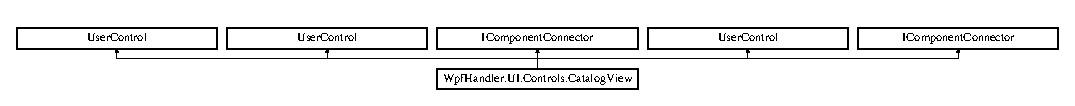
\includegraphics[height=0.982456cm]{dc/db6/class_wpf_handler_1_1_u_i_1_1_controls_1_1_catalog_view}
\end{center}
\end{figure}
\subsection*{Public Member Functions}
\begin{DoxyCompactItemize}
\item 
void \mbox{\hyperlink{class_wpf_handler_1_1_u_i_1_1_controls_1_1_catalog_view_a90654c67633bf7c8848f2b8dc1a3c712}{Initialize\+Component}} ()
\begin{DoxyCompactList}\small\item\em Initialize\+Component \end{DoxyCompactList}\item 
void \mbox{\hyperlink{class_wpf_handler_1_1_u_i_1_1_controls_1_1_catalog_view_a90654c67633bf7c8848f2b8dc1a3c712}{Initialize\+Component}} ()
\begin{DoxyCompactList}\small\item\em Initialize\+Component \end{DoxyCompactList}\item 
\mbox{\hyperlink{class_wpf_handler_1_1_u_i_1_1_controls_1_1_catalog_view_a805f93d9e815024d12b2ca2be31ad071}{Catalog\+View}} ()
\begin{DoxyCompactList}\small\item\em A default constructor. \end{DoxyCompactList}\item 
void \mbox{\hyperlink{class_wpf_handler_1_1_u_i_1_1_controls_1_1_catalog_view_aad6922f8af811dedadc8b4b7ea95ef18}{Update\+Catolog}} ()
\begin{DoxyCompactList}\small\item\em Updating the collection of catalog items. \end{DoxyCompactList}\item 
void \mbox{\hyperlink{class_wpf_handler_1_1_u_i_1_1_controls_1_1_catalog_view_a951cea1f55959f899562479d7b2e4490}{Start\+Plugin}} (int index)
\begin{DoxyCompactList}\small\item\em Starting th eplugin by index. \end{DoxyCompactList}\item 
void \mbox{\hyperlink{class_wpf_handler_1_1_u_i_1_1_controls_1_1_catalog_view_ac22dfdce2ff1a076449c33adf17f1dc1}{Start\+Plugin}} (string domain)
\begin{DoxyCompactList}\small\item\em Starting the plugin by a Menu\+Item\+Meta.\+domain value. \end{DoxyCompactList}\end{DoxyCompactItemize}
\subsection*{Package Attributes}
\begin{DoxyCompactItemize}
\item 
\mbox{\Hypertarget{class_wpf_handler_1_1_u_i_1_1_controls_1_1_catalog_view_afa1ca29284af69857b98e9f01fd55cb2}\label{class_wpf_handler_1_1_u_i_1_1_controls_1_1_catalog_view_afa1ca29284af69857b98e9f01fd55cb2}} 
System.\+Windows.\+Controls.\+Items\+Control {\bfseries Main\+Menu}
\end{DoxyCompactItemize}
\subsection*{Properties}
\begin{DoxyCompactItemize}
\item 
Observable\+Collection$<$ \mbox{\hyperlink{interface_wpf_handler_1_1_plugins_1_1_i_plugin}{I\+Plugin}} $>$ \mbox{\hyperlink{class_wpf_handler_1_1_u_i_1_1_controls_1_1_catalog_view_a7672bbed750a86616eb69af0cec22728}{Plugins}}\hspace{0.3cm}{\ttfamily  \mbox{[}get, set\mbox{]}}
\begin{DoxyCompactList}\small\item\em A collection that contains all loaded plugins. \end{DoxyCompactList}\item 
Observable\+Collection$<$ Framework\+Element $>$ \mbox{\hyperlink{class_wpf_handler_1_1_u_i_1_1_controls_1_1_catalog_view_a2cca758ee3885d67264eea318ea83b91}{Menu\+Buttons}}\hspace{0.3cm}{\ttfamily  \mbox{[}get, protected set\mbox{]}}
\begin{DoxyCompactList}\small\item\em A collection that contains menu\textquotesingle{}s controls. \end{DoxyCompactList}\end{DoxyCompactItemize}
\subsection*{Private Member Functions}
\begin{DoxyCompactItemize}
\item 
\mbox{\Hypertarget{class_wpf_handler_1_1_u_i_1_1_controls_1_1_catalog_view_a494d414ffd5a4bc6df0a11e136399b9c}\label{class_wpf_handler_1_1_u_i_1_1_controls_1_1_catalog_view_a494d414ffd5a4bc6df0a11e136399b9c}} 
void System.\+Windows.\+Markup.\+I\+Component\+Connector. {\bfseries Connect} (int connection\+Id, object target)
\item 
\mbox{\Hypertarget{class_wpf_handler_1_1_u_i_1_1_controls_1_1_catalog_view_a494d414ffd5a4bc6df0a11e136399b9c}\label{class_wpf_handler_1_1_u_i_1_1_controls_1_1_catalog_view_a494d414ffd5a4bc6df0a11e136399b9c}} 
void System.\+Windows.\+Markup.\+I\+Component\+Connector. {\bfseries Connect} (int connection\+Id, object target)
\end{DoxyCompactItemize}
\subsection*{Private Attributes}
\begin{DoxyCompactItemize}
\item 
\mbox{\Hypertarget{class_wpf_handler_1_1_u_i_1_1_controls_1_1_catalog_view_a4919c5ea75e5c986e98266ef8fced0f5}\label{class_wpf_handler_1_1_u_i_1_1_controls_1_1_catalog_view_a4919c5ea75e5c986e98266ef8fced0f5}} 
bool {\bfseries \+\_\+content\+Loaded}
\end{DoxyCompactItemize}


\subsection{Detailed Description}
\mbox{\hyperlink{class_wpf_handler_1_1_u_i_1_1_controls_1_1_catalog_view}{Catalog\+View}} 

Interaction logic for Catalog\+View.\+xaml 

\subsection{Constructor \& Destructor Documentation}
\mbox{\Hypertarget{class_wpf_handler_1_1_u_i_1_1_controls_1_1_catalog_view_a805f93d9e815024d12b2ca2be31ad071}\label{class_wpf_handler_1_1_u_i_1_1_controls_1_1_catalog_view_a805f93d9e815024d12b2ca2be31ad071}} 
\index{Wpf\+Handler\+::\+U\+I\+::\+Controls\+::\+Catalog\+View@{Wpf\+Handler\+::\+U\+I\+::\+Controls\+::\+Catalog\+View}!Catalog\+View@{Catalog\+View}}
\index{Catalog\+View@{Catalog\+View}!Wpf\+Handler\+::\+U\+I\+::\+Controls\+::\+Catalog\+View@{Wpf\+Handler\+::\+U\+I\+::\+Controls\+::\+Catalog\+View}}
\subsubsection{\texorpdfstring{Catalog\+View()}{CatalogView()}}
{\footnotesize\ttfamily Wpf\+Handler.\+U\+I.\+Controls.\+Catalog\+View.\+Catalog\+View (\begin{DoxyParamCaption}{ }\end{DoxyParamCaption})}



A default constructor. 



\subsection{Member Function Documentation}
\mbox{\Hypertarget{class_wpf_handler_1_1_u_i_1_1_controls_1_1_catalog_view_a90654c67633bf7c8848f2b8dc1a3c712}\label{class_wpf_handler_1_1_u_i_1_1_controls_1_1_catalog_view_a90654c67633bf7c8848f2b8dc1a3c712}} 
\index{Wpf\+Handler\+::\+U\+I\+::\+Controls\+::\+Catalog\+View@{Wpf\+Handler\+::\+U\+I\+::\+Controls\+::\+Catalog\+View}!Initialize\+Component@{Initialize\+Component}}
\index{Initialize\+Component@{Initialize\+Component}!Wpf\+Handler\+::\+U\+I\+::\+Controls\+::\+Catalog\+View@{Wpf\+Handler\+::\+U\+I\+::\+Controls\+::\+Catalog\+View}}
\subsubsection{\texorpdfstring{Initialize\+Component()}{InitializeComponent()}\hspace{0.1cm}{\footnotesize\ttfamily [1/2]}}
{\footnotesize\ttfamily void Wpf\+Handler.\+U\+I.\+Controls.\+Catalog\+View.\+Initialize\+Component (\begin{DoxyParamCaption}{ }\end{DoxyParamCaption})}



Initialize\+Component 

\mbox{\Hypertarget{class_wpf_handler_1_1_u_i_1_1_controls_1_1_catalog_view_a90654c67633bf7c8848f2b8dc1a3c712}\label{class_wpf_handler_1_1_u_i_1_1_controls_1_1_catalog_view_a90654c67633bf7c8848f2b8dc1a3c712}} 
\index{Wpf\+Handler\+::\+U\+I\+::\+Controls\+::\+Catalog\+View@{Wpf\+Handler\+::\+U\+I\+::\+Controls\+::\+Catalog\+View}!Initialize\+Component@{Initialize\+Component}}
\index{Initialize\+Component@{Initialize\+Component}!Wpf\+Handler\+::\+U\+I\+::\+Controls\+::\+Catalog\+View@{Wpf\+Handler\+::\+U\+I\+::\+Controls\+::\+Catalog\+View}}
\subsubsection{\texorpdfstring{Initialize\+Component()}{InitializeComponent()}\hspace{0.1cm}{\footnotesize\ttfamily [2/2]}}
{\footnotesize\ttfamily void Wpf\+Handler.\+U\+I.\+Controls.\+Catalog\+View.\+Initialize\+Component (\begin{DoxyParamCaption}{ }\end{DoxyParamCaption})}



Initialize\+Component 

\mbox{\Hypertarget{class_wpf_handler_1_1_u_i_1_1_controls_1_1_catalog_view_a951cea1f55959f899562479d7b2e4490}\label{class_wpf_handler_1_1_u_i_1_1_controls_1_1_catalog_view_a951cea1f55959f899562479d7b2e4490}} 
\index{Wpf\+Handler\+::\+U\+I\+::\+Controls\+::\+Catalog\+View@{Wpf\+Handler\+::\+U\+I\+::\+Controls\+::\+Catalog\+View}!Start\+Plugin@{Start\+Plugin}}
\index{Start\+Plugin@{Start\+Plugin}!Wpf\+Handler\+::\+U\+I\+::\+Controls\+::\+Catalog\+View@{Wpf\+Handler\+::\+U\+I\+::\+Controls\+::\+Catalog\+View}}
\subsubsection{\texorpdfstring{Start\+Plugin()}{StartPlugin()}\hspace{0.1cm}{\footnotesize\ttfamily [1/2]}}
{\footnotesize\ttfamily void Wpf\+Handler.\+U\+I.\+Controls.\+Catalog\+View.\+Start\+Plugin (\begin{DoxyParamCaption}\item[{int}]{index }\end{DoxyParamCaption})}



Starting th eplugin by index. 


\begin{DoxyParams}{Parameters}
{\em index} & Index of the loaded plugin.\\
\hline
\end{DoxyParams}

\begin{DoxyExceptions}{Exceptions}
{\em Index\+Out\+Of\+Range\+Exception} & Occurs when index not valid relative for a loaded plugins list. \\
\hline
\end{DoxyExceptions}
\mbox{\Hypertarget{class_wpf_handler_1_1_u_i_1_1_controls_1_1_catalog_view_ac22dfdce2ff1a076449c33adf17f1dc1}\label{class_wpf_handler_1_1_u_i_1_1_controls_1_1_catalog_view_ac22dfdce2ff1a076449c33adf17f1dc1}} 
\index{Wpf\+Handler\+::\+U\+I\+::\+Controls\+::\+Catalog\+View@{Wpf\+Handler\+::\+U\+I\+::\+Controls\+::\+Catalog\+View}!Start\+Plugin@{Start\+Plugin}}
\index{Start\+Plugin@{Start\+Plugin}!Wpf\+Handler\+::\+U\+I\+::\+Controls\+::\+Catalog\+View@{Wpf\+Handler\+::\+U\+I\+::\+Controls\+::\+Catalog\+View}}
\subsubsection{\texorpdfstring{Start\+Plugin()}{StartPlugin()}\hspace{0.1cm}{\footnotesize\ttfamily [2/2]}}
{\footnotesize\ttfamily void Wpf\+Handler.\+U\+I.\+Controls.\+Catalog\+View.\+Start\+Plugin (\begin{DoxyParamCaption}\item[{string}]{domain }\end{DoxyParamCaption})}



Starting the plugin by a Menu\+Item\+Meta.\+domain value. 


\begin{DoxyParams}{Parameters}
{\em domain} & A plugins\textquotesingle{}s domain name.\\
\hline
\end{DoxyParams}

\begin{DoxyExceptions}{Exceptions}
{\em Key\+Not\+Found\+Exception} & Occurs in case if the domain not found among loaded plugins. \\
\hline
\end{DoxyExceptions}
\mbox{\Hypertarget{class_wpf_handler_1_1_u_i_1_1_controls_1_1_catalog_view_aad6922f8af811dedadc8b4b7ea95ef18}\label{class_wpf_handler_1_1_u_i_1_1_controls_1_1_catalog_view_aad6922f8af811dedadc8b4b7ea95ef18}} 
\index{Wpf\+Handler\+::\+U\+I\+::\+Controls\+::\+Catalog\+View@{Wpf\+Handler\+::\+U\+I\+::\+Controls\+::\+Catalog\+View}!Update\+Catolog@{Update\+Catolog}}
\index{Update\+Catolog@{Update\+Catolog}!Wpf\+Handler\+::\+U\+I\+::\+Controls\+::\+Catalog\+View@{Wpf\+Handler\+::\+U\+I\+::\+Controls\+::\+Catalog\+View}}
\subsubsection{\texorpdfstring{Update\+Catolog()}{UpdateCatolog()}}
{\footnotesize\ttfamily void Wpf\+Handler.\+U\+I.\+Controls.\+Catalog\+View.\+Update\+Catolog (\begin{DoxyParamCaption}{ }\end{DoxyParamCaption})}



Updating the collection of catalog items. 



\subsection{Property Documentation}
\mbox{\Hypertarget{class_wpf_handler_1_1_u_i_1_1_controls_1_1_catalog_view_a2cca758ee3885d67264eea318ea83b91}\label{class_wpf_handler_1_1_u_i_1_1_controls_1_1_catalog_view_a2cca758ee3885d67264eea318ea83b91}} 
\index{Wpf\+Handler\+::\+U\+I\+::\+Controls\+::\+Catalog\+View@{Wpf\+Handler\+::\+U\+I\+::\+Controls\+::\+Catalog\+View}!Menu\+Buttons@{Menu\+Buttons}}
\index{Menu\+Buttons@{Menu\+Buttons}!Wpf\+Handler\+::\+U\+I\+::\+Controls\+::\+Catalog\+View@{Wpf\+Handler\+::\+U\+I\+::\+Controls\+::\+Catalog\+View}}
\subsubsection{\texorpdfstring{Menu\+Buttons}{MenuButtons}}
{\footnotesize\ttfamily Observable\+Collection$<$Framework\+Element$>$ Wpf\+Handler.\+U\+I.\+Controls.\+Catalog\+View.\+Menu\+Buttons\hspace{0.3cm}{\ttfamily [get]}, {\ttfamily [protected set]}}

{\bfseries Initial value\+:}
\begin{DoxyCode}
=
            \textcolor{keyword}{new} ObservableCollection<FrameworkElement>()
\end{DoxyCode}


A collection that contains menu\textquotesingle{}s controls. 

\mbox{\Hypertarget{class_wpf_handler_1_1_u_i_1_1_controls_1_1_catalog_view_a7672bbed750a86616eb69af0cec22728}\label{class_wpf_handler_1_1_u_i_1_1_controls_1_1_catalog_view_a7672bbed750a86616eb69af0cec22728}} 
\index{Wpf\+Handler\+::\+U\+I\+::\+Controls\+::\+Catalog\+View@{Wpf\+Handler\+::\+U\+I\+::\+Controls\+::\+Catalog\+View}!Plugins@{Plugins}}
\index{Plugins@{Plugins}!Wpf\+Handler\+::\+U\+I\+::\+Controls\+::\+Catalog\+View@{Wpf\+Handler\+::\+U\+I\+::\+Controls\+::\+Catalog\+View}}
\subsubsection{\texorpdfstring{Plugins}{Plugins}}
{\footnotesize\ttfamily Observable\+Collection$<$\mbox{\hyperlink{interface_wpf_handler_1_1_plugins_1_1_i_plugin}{I\+Plugin}}$>$ Wpf\+Handler.\+U\+I.\+Controls.\+Catalog\+View.\+Plugins\hspace{0.3cm}{\ttfamily [get]}, {\ttfamily [set]}}



A collection that contains all loaded plugins. 



The documentation for this class was generated from the following files\+:\begin{DoxyCompactItemize}
\item 
D\+:/\+Work/\+Git\+Hub/wpf-\/handler/\+Wpf\+Handler/obj/\+Debug/\+U\+I/\+Controls/Catalog\+View.\+g.\+cs\item 
D\+:/\+Work/\+Git\+Hub/wpf-\/handler/\+Wpf\+Handler/obj/\+Debug/\+U\+I/\+Controls/Catalog\+View.\+g.\+i.\+cs\item 
D\+:/\+Work/\+Git\+Hub/wpf-\/handler/\+Wpf\+Handler/\+U\+I/\+Controls/Catalog\+View.\+xaml.\+cs\end{DoxyCompactItemize}

\hypertarget{class_wpf_handler_1_1_u_i_1_1_controls_1_1_collection_control}{}\section{Wpf\+Handler.\+U\+I.\+Controls.\+Collection\+Control Class Reference}
\label{class_wpf_handler_1_1_u_i_1_1_controls_1_1_collection_control}\index{Wpf\+Handler.\+U\+I.\+Controls.\+Collection\+Control@{Wpf\+Handler.\+U\+I.\+Controls.\+Collection\+Control}}


Abstract class that provides common A\+PI for implementin collection controls.  


Inheritance diagram for Wpf\+Handler.\+U\+I.\+Controls.\+Collection\+Control\+:\begin{figure}[H]
\begin{center}
\leavevmode
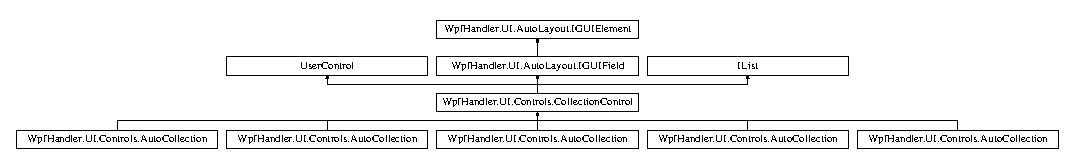
\includegraphics[height=1.763780cm]{d5/d8b/class_wpf_handler_1_1_u_i_1_1_controls_1_1_collection_control}
\end{center}
\end{figure}
\subsection*{Public Member Functions}
\begin{DoxyCompactItemize}
\item 
\mbox{\hyperlink{class_wpf_handler_1_1_u_i_1_1_controls_1_1_collection_control_a5228b3f2d5efec75b178a160bfd9a558}{Collection\+Control}} ()
\begin{DoxyCompactList}\small\item\em Default constructor. \end{DoxyCompactList}\item 
int \mbox{\hyperlink{class_wpf_handler_1_1_u_i_1_1_controls_1_1_collection_control_ae17242c33bd29c2545a06bba9c93a1df}{Add}} (object value)
\begin{DoxyCompactList}\small\item\em Adds an item to the System.\+Collections.\+I\+List. \end{DoxyCompactList}\item 
bool \mbox{\hyperlink{class_wpf_handler_1_1_u_i_1_1_controls_1_1_collection_control_ae703be50b290be72a7a40acbfe65b04c}{Contains}} (object value)
\begin{DoxyCompactList}\small\item\em Determines whether the System.\+Collections.\+I\+List contains a specific value. \end{DoxyCompactList}\item 
void \mbox{\hyperlink{class_wpf_handler_1_1_u_i_1_1_controls_1_1_collection_control_a1f1a7fd996c4e15ec7fe3b2724e962d3}{Clear}} ()
\begin{DoxyCompactList}\small\item\em Removes all items from the System.\+Collections.\+I\+List. \end{DoxyCompactList}\item 
int \mbox{\hyperlink{class_wpf_handler_1_1_u_i_1_1_controls_1_1_collection_control_ad2021b989a7f5aae430e12727a918982}{Index\+Of}} (object value)
\begin{DoxyCompactList}\small\item\em Determines the index of a specific item in the System.\+Collections.\+I\+List. \end{DoxyCompactList}\item 
void \mbox{\hyperlink{class_wpf_handler_1_1_u_i_1_1_controls_1_1_collection_control_ae89cb3b260d441186bac7ee953f4c028}{Insert}} (int index, object value)
\begin{DoxyCompactList}\small\item\em Inserts an item to the System.\+Collections.\+I\+List at the specified index. \end{DoxyCompactList}\item 
void \mbox{\hyperlink{class_wpf_handler_1_1_u_i_1_1_controls_1_1_collection_control_acc5c3b3a95e4d58b6cda68e5f61089fd}{Remove}} (object value)
\begin{DoxyCompactList}\small\item\em Removes the first occurrence of a specific object from the System.\+Collections.\+I\+List. \end{DoxyCompactList}\item 
void \mbox{\hyperlink{class_wpf_handler_1_1_u_i_1_1_controls_1_1_collection_control_ab9ea70c06d17283a4e07195b0f9b0de7}{Remove\+At}} (int index)
\begin{DoxyCompactList}\small\item\em Removes the System.\+Collections.\+I\+List item at the specified index. \end{DoxyCompactList}\item 
void \mbox{\hyperlink{class_wpf_handler_1_1_u_i_1_1_controls_1_1_collection_control_a1cf65910d88b69192fd7dd764a63609a}{Copy\+To}} (Array array, int index)
\begin{DoxyCompactList}\small\item\em Copies the elements of the \mbox{\hyperlink{class_wpf_handler_1_1_u_i_1_1_controls_1_1_collection_control_a78ccfdc5208ab2306308d7356757f32f}{source}} to an System.\+Array, starting at a particular System.\+Array index. \end{DoxyCompactList}\item 
I\+Enumerator \mbox{\hyperlink{class_wpf_handler_1_1_u_i_1_1_controls_1_1_collection_control_a63509ef1e8df1c4901f3b83ff9473236}{Get\+Enumerator}} ()
\begin{DoxyCompactList}\small\item\em Returns an enumerator that iterates through a collection. \end{DoxyCompactList}\item 
virtual void \mbox{\hyperlink{class_wpf_handler_1_1_u_i_1_1_controls_1_1_collection_control_a54cf416fee122e600059ed8713d75bb0}{On\+Layout}} (ref \mbox{\hyperlink{class_wpf_handler_1_1_u_i_1_1_auto_layout_1_1_layout_layer}{Layout\+Layer}} layer, params object\mbox{[}$\,$\mbox{]} args)
\begin{DoxyCompactList}\small\item\em Configurating collection and binding element to the descriptors handler. \end{DoxyCompactList}\end{DoxyCompactItemize}
\subsection*{Public Attributes}
\begin{DoxyCompactItemize}
\item 
bool \mbox{\hyperlink{class_wpf_handler_1_1_u_i_1_1_controls_1_1_collection_control_a2e1f163821f2cbc367ef40d3dcf652eb}{Is\+Read\+Only}} =$>$ \mbox{\hyperlink{class_wpf_handler_1_1_u_i_1_1_controls_1_1_collection_control_a78ccfdc5208ab2306308d7356757f32f}{source}} != null ? source.\+Is\+Read\+Only \+: true
\begin{DoxyCompactList}\small\item\em Gets a value indicating whether the System.\+Collections.\+I\+List is read-\/only. \end{DoxyCompactList}\item 
bool \mbox{\hyperlink{class_wpf_handler_1_1_u_i_1_1_controls_1_1_collection_control_aa95fcae30ed2356bfff8154bcceecc8a}{Is\+Fixed\+Size}} =$>$ \mbox{\hyperlink{class_wpf_handler_1_1_u_i_1_1_controls_1_1_collection_control_a78ccfdc5208ab2306308d7356757f32f}{source}} != null ? source.\+Is\+Fixed\+Size \+: true
\begin{DoxyCompactList}\small\item\em Gets a value indicating whether the System.\+Collections.\+I\+List has a fixed size. \end{DoxyCompactList}\item 
int \mbox{\hyperlink{class_wpf_handler_1_1_u_i_1_1_controls_1_1_collection_control_af4796b6959bcb870bde22f6d32379242}{Count}} =$>$ \mbox{\hyperlink{class_wpf_handler_1_1_u_i_1_1_controls_1_1_collection_control_a78ccfdc5208ab2306308d7356757f32f}{source}} != null ? source.\+Count \+: -\/1
\begin{DoxyCompactList}\small\item\em Gets the number of elements contained in the System.\+Collections.\+I\+Collection. Returns -\/1 in case if source not binded. \end{DoxyCompactList}\item 
object \mbox{\hyperlink{class_wpf_handler_1_1_u_i_1_1_controls_1_1_collection_control_a4ab9c597654cf0ca762f2fa13e807fc7}{Sync\+Root}} =$>$ \mbox{\hyperlink{class_wpf_handler_1_1_u_i_1_1_controls_1_1_collection_control_a78ccfdc5208ab2306308d7356757f32f}{source}}?.Sync\+Root
\begin{DoxyCompactList}\small\item\em Gets an object that can be used to synchronize access to the System.\+Collections.\+I\+Collection. \end{DoxyCompactList}\item 
bool \mbox{\hyperlink{class_wpf_handler_1_1_u_i_1_1_controls_1_1_collection_control_a0a40907daa815eb6c01be8677eb09450}{Is\+Synchronized}} =$>$ \mbox{\hyperlink{class_wpf_handler_1_1_u_i_1_1_controls_1_1_collection_control_a78ccfdc5208ab2306308d7356757f32f}{source}} != null ? source.\+Is\+Fixed\+Size \+: true
\begin{DoxyCompactList}\small\item\em Gets a value indicating whether access to the System.\+Collections.\+I\+Collection is synchronized (thread safe). \end{DoxyCompactList}\end{DoxyCompactItemize}
\subsection*{Static Public Attributes}
\begin{DoxyCompactItemize}
\item 
static readonly Dependency\+Property \mbox{\hyperlink{class_wpf_handler_1_1_u_i_1_1_controls_1_1_collection_control_aea4afe7ae229937f9c99809d720d8875}{Drag\+Allowed\+Property}}
\begin{DoxyCompactList}\small\item\em Property that bridging control\textquotesingle{}s property between X\+A\+ML and code. \end{DoxyCompactList}\end{DoxyCompactItemize}
\subsection*{Protected Member Functions}
\begin{DoxyCompactItemize}
\item 
void \mbox{\hyperlink{class_wpf_handler_1_1_u_i_1_1_controls_1_1_collection_control_a6df510adc9706b127f2179a6cc123799}{Update\+Elements\+Width}} (object sender, Size\+Changed\+Event\+Args e)
\begin{DoxyCompactList}\small\item\em Requiesting recomputing of the elements width. \end{DoxyCompactList}\item 
void \mbox{\hyperlink{class_wpf_handler_1_1_u_i_1_1_controls_1_1_collection_control_a5fdb64f8a451f387f2a36686f0fec014}{Configurate\+Styles}} ()
\begin{DoxyCompactList}\small\item\em Configurating styles applyed to the controls. \end{DoxyCompactList}\item 
virtual Framework\+Element \mbox{\hyperlink{class_wpf_handler_1_1_u_i_1_1_controls_1_1_collection_control_af375cbcb4d351b4d104b2706d39b8303}{Item\+Registration}} (int index)
\begin{DoxyCompactList}\small\item\em Regestrating element for source collection. Allow to create bachward binding of \mbox{\hyperlink{namespace_wpf_handler_1_1_u_i}{UI}} to the source object. \end{DoxyCompactList}\item 
virtual void \mbox{\hyperlink{class_wpf_handler_1_1_u_i_1_1_controls_1_1_collection_control_a2372fa8b10c175bb81d5901f36cbf8f7}{Collection\+Element\+Value\+Changed}} (\mbox{\hyperlink{interface_wpf_handler_1_1_u_i_1_1_auto_layout_1_1_i_g_u_i_field}{I\+G\+U\+I\+Field}} obj)
\begin{DoxyCompactList}\small\item\em Occurs when field\textquotesingle{}s valu will be changed via \mbox{\hyperlink{namespace_wpf_handler_1_1_u_i}{UI}} element. \end{DoxyCompactList}\item 
virtual void \mbox{\hyperlink{class_wpf_handler_1_1_u_i_1_1_controls_1_1_collection_control_ad6c991f82c204e789f32f21d28d48524}{On\+Preview\+Mouse\+Left\+Button\+Down}} (object sender, Mouse\+Button\+Event\+Args e)
\begin{DoxyCompactList}\small\item\em Occurs when item is selected by L\+MB click. \end{DoxyCompactList}\item 
virtual void \mbox{\hyperlink{class_wpf_handler_1_1_u_i_1_1_controls_1_1_collection_control_ae52c8e47654ca10e714a1e87a193331b}{On\+Item\+Drop}} (object sender, Drag\+Event\+Args e)
\begin{DoxyCompactList}\small\item\em Occurs when an element was droped after drag. \end{DoxyCompactList}\end{DoxyCompactItemize}
\subsection*{Protected Attributes}
\begin{DoxyCompactItemize}
\item 
readonly Hashtable \mbox{\hyperlink{class_wpf_handler_1_1_u_i_1_1_controls_1_1_collection_control_af3a8d4c03474bbb80d8d461f4a8e33e8}{index\+Map}} = new Hashtable()
\begin{DoxyCompactList}\small\item\em Mapp of G\+UI elements binding. I\+G\+U\+I\+Field -\/ key int -\/ index in the list. \end{DoxyCompactList}\item 
I\+List \mbox{\hyperlink{class_wpf_handler_1_1_u_i_1_1_controls_1_1_collection_control_a78ccfdc5208ab2306308d7356757f32f}{source}}
\begin{DoxyCompactList}\small\item\em Bufer that contains source sollection. \end{DoxyCompactList}\item 
I\+List \mbox{\hyperlink{class_wpf_handler_1_1_u_i_1_1_controls_1_1_collection_control_a128726ac8376cf78e3c33ba1c9f00b2d}{binded\+Source}}
\begin{DoxyCompactList}\small\item\em Source that is binded to the current \mbox{\hyperlink{namespace_wpf_handler_1_1_u_i}{UI}}. \end{DoxyCompactList}\end{DoxyCompactItemize}
\subsection*{Properties}
\begin{DoxyCompactItemize}
\item 
virtual bool \mbox{\hyperlink{class_wpf_handler_1_1_u_i_1_1_controls_1_1_collection_control_a93748b307999d44bfa539f0a799af1de}{Drag\+Allowed}}\hspace{0.3cm}{\ttfamily  \mbox{[}get, set\mbox{]}}
\begin{DoxyCompactList}\small\item\em Is list allows to drag elements. \end{DoxyCompactList}\item 
abstract List\+Box \mbox{\hyperlink{class_wpf_handler_1_1_u_i_1_1_controls_1_1_collection_control_af98966a5a52deff891275181f1a82b17}{List\+Content}}\hspace{0.3cm}{\ttfamily  \mbox{[}get\mbox{]}}
\begin{DoxyCompactList}\small\item\em Reference to the list box that will contains spawned elements. \end{DoxyCompactList}\item 
object \mbox{\hyperlink{class_wpf_handler_1_1_u_i_1_1_controls_1_1_collection_control_a130ec8fe8e45683069833138833e9356}{Value}}\hspace{0.3cm}{\ttfamily  \mbox{[}get, set\mbox{]}}
\begin{DoxyCompactList}\small\item\em Source collection applied to the \mbox{\hyperlink{namespace_wpf_handler_1_1_u_i}{UI}}. \end{DoxyCompactList}\item 
Member\+Info \mbox{\hyperlink{class_wpf_handler_1_1_u_i_1_1_controls_1_1_collection_control_ac5f779f05470058d2506b4f37cade718}{Binded\+Member}}\hspace{0.3cm}{\ttfamily  \mbox{[}get, set\mbox{]}}
\begin{DoxyCompactList}\small\item\em Member from U\+I\+Descriptor binded to the \mbox{\hyperlink{namespace_wpf_handler_1_1_u_i}{UI}} leement. \end{DoxyCompactList}\item 
Observable\+Collection$<$ Framework\+Element $>$ \mbox{\hyperlink{class_wpf_handler_1_1_u_i_1_1_controls_1_1_collection_control_ade5772e31978f3f8764f50d7483d27f4}{Elements}} = new Observable\+Collection$<$Framework\+Element$>$()\hspace{0.3cm}{\ttfamily  \mbox{[}get\mbox{]}}
\begin{DoxyCompactList}\small\item\em \mbox{\hyperlink{namespace_wpf_handler_1_1_u_i}{UI}} elemets existing into the current collection. \end{DoxyCompactList}\item 
Observable\+Collection$<$ \mbox{\hyperlink{interface_wpf_handler_1_1_u_i_1_1_auto_layout_1_1_i_g_u_i_field}{I\+G\+U\+I\+Field}} $>$ \mbox{\hyperlink{class_wpf_handler_1_1_u_i_1_1_controls_1_1_collection_control_a47291558ce667430c006d9e294f714bb}{Fields}} = new Observable\+Collection$<$\mbox{\hyperlink{interface_wpf_handler_1_1_u_i_1_1_auto_layout_1_1_i_g_u_i_field}{I\+G\+U\+I\+Field}}$>$()\hspace{0.3cm}{\ttfamily  \mbox{[}get\mbox{]}}
\begin{DoxyCompactList}\small\item\em Collection that contains instiniated G\+UI fields. \end{DoxyCompactList}\item 
object \mbox{\hyperlink{class_wpf_handler_1_1_u_i_1_1_controls_1_1_collection_control_ade95cee1fcd80188e8b5e5a15b33d43f}{this\mbox{[}int index\mbox{]}}}\hspace{0.3cm}{\ttfamily  \mbox{[}get, set\mbox{]}}
\begin{DoxyCompactList}\small\item\em Gets or sets the element at the specified index. \end{DoxyCompactList}\end{DoxyCompactItemize}
\subsection*{Events}
\begin{DoxyCompactItemize}
\item 
Action$<$ \mbox{\hyperlink{interface_wpf_handler_1_1_u_i_1_1_auto_layout_1_1_i_g_u_i_field}{I\+G\+U\+I\+Field}} $>$ \mbox{\hyperlink{class_wpf_handler_1_1_u_i_1_1_controls_1_1_collection_control_a7c24ead5af7dadce18f017f0a93706a2}{Value\+Changed}}
\begin{DoxyCompactList}\small\item\em Will occure when source or one from elements will change. \end{DoxyCompactList}\end{DoxyCompactItemize}


\subsection{Detailed Description}
Abstract class that provides common A\+PI for implementin collection controls. 

Fully compatible with U\+I\+Descriptor and auto layout handlers. 

\subsection{Constructor \& Destructor Documentation}
\mbox{\Hypertarget{class_wpf_handler_1_1_u_i_1_1_controls_1_1_collection_control_a5228b3f2d5efec75b178a160bfd9a558}\label{class_wpf_handler_1_1_u_i_1_1_controls_1_1_collection_control_a5228b3f2d5efec75b178a160bfd9a558}} 
\index{Wpf\+Handler\+::\+U\+I\+::\+Controls\+::\+Collection\+Control@{Wpf\+Handler\+::\+U\+I\+::\+Controls\+::\+Collection\+Control}!Collection\+Control@{Collection\+Control}}
\index{Collection\+Control@{Collection\+Control}!Wpf\+Handler\+::\+U\+I\+::\+Controls\+::\+Collection\+Control@{Wpf\+Handler\+::\+U\+I\+::\+Controls\+::\+Collection\+Control}}
\subsubsection{\texorpdfstring{Collection\+Control()}{CollectionControl()}}
{\footnotesize\ttfamily Wpf\+Handler.\+U\+I.\+Controls.\+Collection\+Control.\+Collection\+Control (\begin{DoxyParamCaption}{ }\end{DoxyParamCaption})}



Default constructor. 



\subsection{Member Function Documentation}
\mbox{\Hypertarget{class_wpf_handler_1_1_u_i_1_1_controls_1_1_collection_control_ae17242c33bd29c2545a06bba9c93a1df}\label{class_wpf_handler_1_1_u_i_1_1_controls_1_1_collection_control_ae17242c33bd29c2545a06bba9c93a1df}} 
\index{Wpf\+Handler\+::\+U\+I\+::\+Controls\+::\+Collection\+Control@{Wpf\+Handler\+::\+U\+I\+::\+Controls\+::\+Collection\+Control}!Add@{Add}}
\index{Add@{Add}!Wpf\+Handler\+::\+U\+I\+::\+Controls\+::\+Collection\+Control@{Wpf\+Handler\+::\+U\+I\+::\+Controls\+::\+Collection\+Control}}
\subsubsection{\texorpdfstring{Add()}{Add()}}
{\footnotesize\ttfamily int Wpf\+Handler.\+U\+I.\+Controls.\+Collection\+Control.\+Add (\begin{DoxyParamCaption}\item[{object}]{value }\end{DoxyParamCaption})}



Adds an item to the System.\+Collections.\+I\+List. 


\begin{DoxyParams}{Parameters}
{\em value} & The object to add to the System.\+Collections.\+I\+List.\\
\hline
\end{DoxyParams}
\begin{DoxyReturn}{Returns}
The position into which the new element was inserted, or -\/1 to indicate that the item was not inserted into the collection. 
\end{DoxyReturn}

\begin{DoxyExceptions}{Exceptions}
{\em System.\+Not\+Supported\+Exception} & The System.\+Collections.\+I\+List is read-\/only.-\/or-\/ The System.\+Collections.\+I\+List has a fixed size.-\/or-\/ I\+G\+U\+I\+Field for the object type not registred. \\
\hline
\end{DoxyExceptions}
\mbox{\Hypertarget{class_wpf_handler_1_1_u_i_1_1_controls_1_1_collection_control_a1f1a7fd996c4e15ec7fe3b2724e962d3}\label{class_wpf_handler_1_1_u_i_1_1_controls_1_1_collection_control_a1f1a7fd996c4e15ec7fe3b2724e962d3}} 
\index{Wpf\+Handler\+::\+U\+I\+::\+Controls\+::\+Collection\+Control@{Wpf\+Handler\+::\+U\+I\+::\+Controls\+::\+Collection\+Control}!Clear@{Clear}}
\index{Clear@{Clear}!Wpf\+Handler\+::\+U\+I\+::\+Controls\+::\+Collection\+Control@{Wpf\+Handler\+::\+U\+I\+::\+Controls\+::\+Collection\+Control}}
\subsubsection{\texorpdfstring{Clear()}{Clear()}}
{\footnotesize\ttfamily void Wpf\+Handler.\+U\+I.\+Controls.\+Collection\+Control.\+Clear (\begin{DoxyParamCaption}{ }\end{DoxyParamCaption})}



Removes all items from the System.\+Collections.\+I\+List. 


\begin{DoxyExceptions}{Exceptions}
{\em System.\+Not\+Supported\+Exception} & The System.\+Collections.\+I\+List is read-\/only. \\
\hline
\end{DoxyExceptions}
\mbox{\Hypertarget{class_wpf_handler_1_1_u_i_1_1_controls_1_1_collection_control_a2372fa8b10c175bb81d5901f36cbf8f7}\label{class_wpf_handler_1_1_u_i_1_1_controls_1_1_collection_control_a2372fa8b10c175bb81d5901f36cbf8f7}} 
\index{Wpf\+Handler\+::\+U\+I\+::\+Controls\+::\+Collection\+Control@{Wpf\+Handler\+::\+U\+I\+::\+Controls\+::\+Collection\+Control}!Collection\+Element\+Value\+Changed@{Collection\+Element\+Value\+Changed}}
\index{Collection\+Element\+Value\+Changed@{Collection\+Element\+Value\+Changed}!Wpf\+Handler\+::\+U\+I\+::\+Controls\+::\+Collection\+Control@{Wpf\+Handler\+::\+U\+I\+::\+Controls\+::\+Collection\+Control}}
\subsubsection{\texorpdfstring{Collection\+Element\+Value\+Changed()}{CollectionElementValueChanged()}}
{\footnotesize\ttfamily virtual void Wpf\+Handler.\+U\+I.\+Controls.\+Collection\+Control.\+Collection\+Element\+Value\+Changed (\begin{DoxyParamCaption}\item[{\mbox{\hyperlink{interface_wpf_handler_1_1_u_i_1_1_auto_layout_1_1_i_g_u_i_field}{I\+G\+U\+I\+Field}}}]{obj }\end{DoxyParamCaption})\hspace{0.3cm}{\ttfamily [protected]}, {\ttfamily [virtual]}}



Occurs when field\textquotesingle{}s valu will be changed via \mbox{\hyperlink{namespace_wpf_handler_1_1_u_i}{UI}} element. 


\begin{DoxyParams}{Parameters}
{\em obj} & The G\+UI element that initialize event.\\
\hline
\end{DoxyParams}
\mbox{\Hypertarget{class_wpf_handler_1_1_u_i_1_1_controls_1_1_collection_control_a5fdb64f8a451f387f2a36686f0fec014}\label{class_wpf_handler_1_1_u_i_1_1_controls_1_1_collection_control_a5fdb64f8a451f387f2a36686f0fec014}} 
\index{Wpf\+Handler\+::\+U\+I\+::\+Controls\+::\+Collection\+Control@{Wpf\+Handler\+::\+U\+I\+::\+Controls\+::\+Collection\+Control}!Configurate\+Styles@{Configurate\+Styles}}
\index{Configurate\+Styles@{Configurate\+Styles}!Wpf\+Handler\+::\+U\+I\+::\+Controls\+::\+Collection\+Control@{Wpf\+Handler\+::\+U\+I\+::\+Controls\+::\+Collection\+Control}}
\subsubsection{\texorpdfstring{Configurate\+Styles()}{ConfigurateStyles()}}
{\footnotesize\ttfamily void Wpf\+Handler.\+U\+I.\+Controls.\+Collection\+Control.\+Configurate\+Styles (\begin{DoxyParamCaption}{ }\end{DoxyParamCaption})\hspace{0.3cm}{\ttfamily [protected]}}



Configurating styles applyed to the controls. 

\mbox{\Hypertarget{class_wpf_handler_1_1_u_i_1_1_controls_1_1_collection_control_ae703be50b290be72a7a40acbfe65b04c}\label{class_wpf_handler_1_1_u_i_1_1_controls_1_1_collection_control_ae703be50b290be72a7a40acbfe65b04c}} 
\index{Wpf\+Handler\+::\+U\+I\+::\+Controls\+::\+Collection\+Control@{Wpf\+Handler\+::\+U\+I\+::\+Controls\+::\+Collection\+Control}!Contains@{Contains}}
\index{Contains@{Contains}!Wpf\+Handler\+::\+U\+I\+::\+Controls\+::\+Collection\+Control@{Wpf\+Handler\+::\+U\+I\+::\+Controls\+::\+Collection\+Control}}
\subsubsection{\texorpdfstring{Contains()}{Contains()}}
{\footnotesize\ttfamily bool Wpf\+Handler.\+U\+I.\+Controls.\+Collection\+Control.\+Contains (\begin{DoxyParamCaption}\item[{object}]{value }\end{DoxyParamCaption})}



Determines whether the System.\+Collections.\+I\+List contains a specific value. 


\begin{DoxyParams}{Parameters}
{\em value} & The object to locate in the System.\+Collections.\+I\+List.\\
\hline
\end{DoxyParams}
\begin{DoxyReturn}{Returns}
true if the System.\+Object is found in the System.\+Collections.\+I\+List; otherwise, false. 
\end{DoxyReturn}


In case if value is I\+G\+U\+I\+Field then looking via registred \mbox{\hyperlink{namespace_wpf_handler_1_1_u_i}{UI}} fileds.-\/or-\/ Otherwise looking via the \mbox{\hyperlink{class_wpf_handler_1_1_u_i_1_1_controls_1_1_collection_control_a78ccfdc5208ab2306308d7356757f32f}{source}} list. \mbox{\Hypertarget{class_wpf_handler_1_1_u_i_1_1_controls_1_1_collection_control_a1cf65910d88b69192fd7dd764a63609a}\label{class_wpf_handler_1_1_u_i_1_1_controls_1_1_collection_control_a1cf65910d88b69192fd7dd764a63609a}} 
\index{Wpf\+Handler\+::\+U\+I\+::\+Controls\+::\+Collection\+Control@{Wpf\+Handler\+::\+U\+I\+::\+Controls\+::\+Collection\+Control}!Copy\+To@{Copy\+To}}
\index{Copy\+To@{Copy\+To}!Wpf\+Handler\+::\+U\+I\+::\+Controls\+::\+Collection\+Control@{Wpf\+Handler\+::\+U\+I\+::\+Controls\+::\+Collection\+Control}}
\subsubsection{\texorpdfstring{Copy\+To()}{CopyTo()}}
{\footnotesize\ttfamily void Wpf\+Handler.\+U\+I.\+Controls.\+Collection\+Control.\+Copy\+To (\begin{DoxyParamCaption}\item[{Array}]{array,  }\item[{int}]{index }\end{DoxyParamCaption})}



Copies the elements of the \mbox{\hyperlink{class_wpf_handler_1_1_u_i_1_1_controls_1_1_collection_control_a78ccfdc5208ab2306308d7356757f32f}{source}} to an System.\+Array, starting at a particular System.\+Array index. 


\begin{DoxyParams}{Parameters}
{\em array} & The one-\/dimensional System.\+Array that is the destination of the elements copied from System.\+Collections.\+I\+Collection. The System.\+Array must have zero-\/based indexing.\\
\hline
{\em index} & The zero-\/based index in array at which copying begins.\\
\hline
\end{DoxyParams}

\begin{DoxyExceptions}{Exceptions}
{\em System.\+Argument\+Null\+Exception} & array is null. \\
\hline
{\em System.\+Argument\+Out\+Of\+Range\+Exception} & index is less than zero. \\
\hline
{\em System.\+Argument\+Null\+Exception} & array is multidimensional.-\/or-\/ The number of elements in the source System.\+Collections.\+I\+Collection is greater than the available space from index to the end of the destination array.-\/or-\/\+The type of the source System.\+Collections.\+I\+Collection cannot be cast automatically to the type of the destination array. \\
\hline
\end{DoxyExceptions}
\mbox{\Hypertarget{class_wpf_handler_1_1_u_i_1_1_controls_1_1_collection_control_a63509ef1e8df1c4901f3b83ff9473236}\label{class_wpf_handler_1_1_u_i_1_1_controls_1_1_collection_control_a63509ef1e8df1c4901f3b83ff9473236}} 
\index{Wpf\+Handler\+::\+U\+I\+::\+Controls\+::\+Collection\+Control@{Wpf\+Handler\+::\+U\+I\+::\+Controls\+::\+Collection\+Control}!Get\+Enumerator@{Get\+Enumerator}}
\index{Get\+Enumerator@{Get\+Enumerator}!Wpf\+Handler\+::\+U\+I\+::\+Controls\+::\+Collection\+Control@{Wpf\+Handler\+::\+U\+I\+::\+Controls\+::\+Collection\+Control}}
\subsubsection{\texorpdfstring{Get\+Enumerator()}{GetEnumerator()}}
{\footnotesize\ttfamily I\+Enumerator Wpf\+Handler.\+U\+I.\+Controls.\+Collection\+Control.\+Get\+Enumerator (\begin{DoxyParamCaption}{ }\end{DoxyParamCaption})}



Returns an enumerator that iterates through a collection. 

\begin{DoxyReturn}{Returns}
An System.\+Collections.\+I\+Enumerator object that can be used to iterate through the collection. 
\end{DoxyReturn}
\mbox{\Hypertarget{class_wpf_handler_1_1_u_i_1_1_controls_1_1_collection_control_ad2021b989a7f5aae430e12727a918982}\label{class_wpf_handler_1_1_u_i_1_1_controls_1_1_collection_control_ad2021b989a7f5aae430e12727a918982}} 
\index{Wpf\+Handler\+::\+U\+I\+::\+Controls\+::\+Collection\+Control@{Wpf\+Handler\+::\+U\+I\+::\+Controls\+::\+Collection\+Control}!Index\+Of@{Index\+Of}}
\index{Index\+Of@{Index\+Of}!Wpf\+Handler\+::\+U\+I\+::\+Controls\+::\+Collection\+Control@{Wpf\+Handler\+::\+U\+I\+::\+Controls\+::\+Collection\+Control}}
\subsubsection{\texorpdfstring{Index\+Of()}{IndexOf()}}
{\footnotesize\ttfamily int Wpf\+Handler.\+U\+I.\+Controls.\+Collection\+Control.\+Index\+Of (\begin{DoxyParamCaption}\item[{object}]{value }\end{DoxyParamCaption})}



Determines the index of a specific item in the System.\+Collections.\+I\+List. 


\begin{DoxyParams}{Parameters}
{\em value} & The object to locate in the System.\+Collections.\+I\+List.\\
\hline
\end{DoxyParams}
\begin{DoxyReturn}{Returns}
The index of value if found in the list; otherwise, -\/1.
\end{DoxyReturn}


In case if value is I\+G\+U\+I\+Field then looking via registred \mbox{\hyperlink{namespace_wpf_handler_1_1_u_i}{UI}} fileds.-\/or-\/ Otherwise looking via the \mbox{\hyperlink{class_wpf_handler_1_1_u_i_1_1_controls_1_1_collection_control_a78ccfdc5208ab2306308d7356757f32f}{source}} list. \mbox{\Hypertarget{class_wpf_handler_1_1_u_i_1_1_controls_1_1_collection_control_ae89cb3b260d441186bac7ee953f4c028}\label{class_wpf_handler_1_1_u_i_1_1_controls_1_1_collection_control_ae89cb3b260d441186bac7ee953f4c028}} 
\index{Wpf\+Handler\+::\+U\+I\+::\+Controls\+::\+Collection\+Control@{Wpf\+Handler\+::\+U\+I\+::\+Controls\+::\+Collection\+Control}!Insert@{Insert}}
\index{Insert@{Insert}!Wpf\+Handler\+::\+U\+I\+::\+Controls\+::\+Collection\+Control@{Wpf\+Handler\+::\+U\+I\+::\+Controls\+::\+Collection\+Control}}
\subsubsection{\texorpdfstring{Insert()}{Insert()}}
{\footnotesize\ttfamily void Wpf\+Handler.\+U\+I.\+Controls.\+Collection\+Control.\+Insert (\begin{DoxyParamCaption}\item[{int}]{index,  }\item[{object}]{value }\end{DoxyParamCaption})}



Inserts an item to the System.\+Collections.\+I\+List at the specified index. 


\begin{DoxyParams}{Parameters}
{\em index} & The zero-\/based index at which value should be inserted.\\
\hline
{\em value} & The object to insert into the System.\+Collections.\+I\+List.\\
\hline
\end{DoxyParams}

\begin{DoxyExceptions}{Exceptions}
{\em System.\+Argument\+Out\+Of\+Range\+Exception} & index is not a valid index in the System.\+Collections.\+I\+List. \\
\hline
{\em System.\+Not\+Supported\+Exception} & The System.\+Collections.\+I\+List is read-\/only.-\/or-\/ The System.\+Collections.\+I\+List has a fixed size. \\
\hline
{\em System.\+Null\+Reference\+Exception} & value is null reference in the System.\+Collections.\+I\+List. \\
\hline
\end{DoxyExceptions}
\mbox{\Hypertarget{class_wpf_handler_1_1_u_i_1_1_controls_1_1_collection_control_af375cbcb4d351b4d104b2706d39b8303}\label{class_wpf_handler_1_1_u_i_1_1_controls_1_1_collection_control_af375cbcb4d351b4d104b2706d39b8303}} 
\index{Wpf\+Handler\+::\+U\+I\+::\+Controls\+::\+Collection\+Control@{Wpf\+Handler\+::\+U\+I\+::\+Controls\+::\+Collection\+Control}!Item\+Registration@{Item\+Registration}}
\index{Item\+Registration@{Item\+Registration}!Wpf\+Handler\+::\+U\+I\+::\+Controls\+::\+Collection\+Control@{Wpf\+Handler\+::\+U\+I\+::\+Controls\+::\+Collection\+Control}}
\subsubsection{\texorpdfstring{Item\+Registration()}{ItemRegistration()}}
{\footnotesize\ttfamily virtual Framework\+Element Wpf\+Handler.\+U\+I.\+Controls.\+Collection\+Control.\+Item\+Registration (\begin{DoxyParamCaption}\item[{int}]{index }\end{DoxyParamCaption})\hspace{0.3cm}{\ttfamily [protected]}, {\ttfamily [virtual]}}



Regestrating element for source collection. Allow to create bachward binding of \mbox{\hyperlink{namespace_wpf_handler_1_1_u_i}{UI}} to the source object. 


\begin{DoxyParams}{Parameters}
{\em index} & Index of the element into the \mbox{\hyperlink{class_wpf_handler_1_1_u_i_1_1_controls_1_1_collection_control_a78ccfdc5208ab2306308d7356757f32f}{source}} collection.\\
\hline
\end{DoxyParams}


Reimplemented in \mbox{\hyperlink{class_wpf_handler_1_1_u_i_1_1_controls_1_1_auto_collection_a7cea6362ca2a31dca7bca6ab1f39142d}{Wpf\+Handler.\+U\+I.\+Controls.\+Auto\+Collection}}.

\mbox{\Hypertarget{class_wpf_handler_1_1_u_i_1_1_controls_1_1_collection_control_ae52c8e47654ca10e714a1e87a193331b}\label{class_wpf_handler_1_1_u_i_1_1_controls_1_1_collection_control_ae52c8e47654ca10e714a1e87a193331b}} 
\index{Wpf\+Handler\+::\+U\+I\+::\+Controls\+::\+Collection\+Control@{Wpf\+Handler\+::\+U\+I\+::\+Controls\+::\+Collection\+Control}!On\+Item\+Drop@{On\+Item\+Drop}}
\index{On\+Item\+Drop@{On\+Item\+Drop}!Wpf\+Handler\+::\+U\+I\+::\+Controls\+::\+Collection\+Control@{Wpf\+Handler\+::\+U\+I\+::\+Controls\+::\+Collection\+Control}}
\subsubsection{\texorpdfstring{On\+Item\+Drop()}{OnItemDrop()}}
{\footnotesize\ttfamily virtual void Wpf\+Handler.\+U\+I.\+Controls.\+Collection\+Control.\+On\+Item\+Drop (\begin{DoxyParamCaption}\item[{object}]{sender,  }\item[{Drag\+Event\+Args}]{e }\end{DoxyParamCaption})\hspace{0.3cm}{\ttfamily [protected]}, {\ttfamily [virtual]}}



Occurs when an element was droped after drag. 


\begin{DoxyParams}{Parameters}
{\em sender} & \\
\hline
{\em e} & \\
\hline
\end{DoxyParams}
\mbox{\Hypertarget{class_wpf_handler_1_1_u_i_1_1_controls_1_1_collection_control_a54cf416fee122e600059ed8713d75bb0}\label{class_wpf_handler_1_1_u_i_1_1_controls_1_1_collection_control_a54cf416fee122e600059ed8713d75bb0}} 
\index{Wpf\+Handler\+::\+U\+I\+::\+Controls\+::\+Collection\+Control@{Wpf\+Handler\+::\+U\+I\+::\+Controls\+::\+Collection\+Control}!On\+Layout@{On\+Layout}}
\index{On\+Layout@{On\+Layout}!Wpf\+Handler\+::\+U\+I\+::\+Controls\+::\+Collection\+Control@{Wpf\+Handler\+::\+U\+I\+::\+Controls\+::\+Collection\+Control}}
\subsubsection{\texorpdfstring{On\+Layout()}{OnLayout()}}
{\footnotesize\ttfamily virtual void Wpf\+Handler.\+U\+I.\+Controls.\+Collection\+Control.\+On\+Layout (\begin{DoxyParamCaption}\item[{ref \mbox{\hyperlink{class_wpf_handler_1_1_u_i_1_1_auto_layout_1_1_layout_layer}{Layout\+Layer}}}]{layer,  }\item[{params object \mbox{[}$\,$\mbox{]}}]{args }\end{DoxyParamCaption})\hspace{0.3cm}{\ttfamily [virtual]}}



Configurating collection and binding element to the descriptors handler. 


\begin{DoxyParams}{Parameters}
{\em layer} & \\
\hline
{\em args} & \\
\hline
\end{DoxyParams}


Implements \mbox{\hyperlink{interface_wpf_handler_1_1_u_i_1_1_auto_layout_1_1_i_g_u_i_element_a0ff16956f8e8187d51e1b36b6b9f894e}{Wpf\+Handler.\+U\+I.\+Auto\+Layout.\+I\+G\+U\+I\+Element}}.

\mbox{\Hypertarget{class_wpf_handler_1_1_u_i_1_1_controls_1_1_collection_control_ad6c991f82c204e789f32f21d28d48524}\label{class_wpf_handler_1_1_u_i_1_1_controls_1_1_collection_control_ad6c991f82c204e789f32f21d28d48524}} 
\index{Wpf\+Handler\+::\+U\+I\+::\+Controls\+::\+Collection\+Control@{Wpf\+Handler\+::\+U\+I\+::\+Controls\+::\+Collection\+Control}!On\+Preview\+Mouse\+Left\+Button\+Down@{On\+Preview\+Mouse\+Left\+Button\+Down}}
\index{On\+Preview\+Mouse\+Left\+Button\+Down@{On\+Preview\+Mouse\+Left\+Button\+Down}!Wpf\+Handler\+::\+U\+I\+::\+Controls\+::\+Collection\+Control@{Wpf\+Handler\+::\+U\+I\+::\+Controls\+::\+Collection\+Control}}
\subsubsection{\texorpdfstring{On\+Preview\+Mouse\+Left\+Button\+Down()}{OnPreviewMouseLeftButtonDown()}}
{\footnotesize\ttfamily virtual void Wpf\+Handler.\+U\+I.\+Controls.\+Collection\+Control.\+On\+Preview\+Mouse\+Left\+Button\+Down (\begin{DoxyParamCaption}\item[{object}]{sender,  }\item[{Mouse\+Button\+Event\+Args}]{e }\end{DoxyParamCaption})\hspace{0.3cm}{\ttfamily [protected]}, {\ttfamily [virtual]}}



Occurs when item is selected by L\+MB click. 


\begin{DoxyParams}{Parameters}
{\em sender} & \\
\hline
{\em e} & \\
\hline
\end{DoxyParams}
\mbox{\Hypertarget{class_wpf_handler_1_1_u_i_1_1_controls_1_1_collection_control_acc5c3b3a95e4d58b6cda68e5f61089fd}\label{class_wpf_handler_1_1_u_i_1_1_controls_1_1_collection_control_acc5c3b3a95e4d58b6cda68e5f61089fd}} 
\index{Wpf\+Handler\+::\+U\+I\+::\+Controls\+::\+Collection\+Control@{Wpf\+Handler\+::\+U\+I\+::\+Controls\+::\+Collection\+Control}!Remove@{Remove}}
\index{Remove@{Remove}!Wpf\+Handler\+::\+U\+I\+::\+Controls\+::\+Collection\+Control@{Wpf\+Handler\+::\+U\+I\+::\+Controls\+::\+Collection\+Control}}
\subsubsection{\texorpdfstring{Remove()}{Remove()}}
{\footnotesize\ttfamily void Wpf\+Handler.\+U\+I.\+Controls.\+Collection\+Control.\+Remove (\begin{DoxyParamCaption}\item[{object}]{value }\end{DoxyParamCaption})}



Removes the first occurrence of a specific object from the System.\+Collections.\+I\+List. 


\begin{DoxyParams}{Parameters}
{\em value} & The object to remove from the System.\+Collections.\+I\+List.\\
\hline
\end{DoxyParams}

\begin{DoxyExceptions}{Exceptions}
{\em System.\+Not\+Supported\+Exception} & The System.\+Collections.\+I\+List is read-\/only.-\/or-\/ The System.\+Collections.\+I\+List has a fixed size. \\
\hline
\end{DoxyExceptions}
\mbox{\Hypertarget{class_wpf_handler_1_1_u_i_1_1_controls_1_1_collection_control_ab9ea70c06d17283a4e07195b0f9b0de7}\label{class_wpf_handler_1_1_u_i_1_1_controls_1_1_collection_control_ab9ea70c06d17283a4e07195b0f9b0de7}} 
\index{Wpf\+Handler\+::\+U\+I\+::\+Controls\+::\+Collection\+Control@{Wpf\+Handler\+::\+U\+I\+::\+Controls\+::\+Collection\+Control}!Remove\+At@{Remove\+At}}
\index{Remove\+At@{Remove\+At}!Wpf\+Handler\+::\+U\+I\+::\+Controls\+::\+Collection\+Control@{Wpf\+Handler\+::\+U\+I\+::\+Controls\+::\+Collection\+Control}}
\subsubsection{\texorpdfstring{Remove\+At()}{RemoveAt()}}
{\footnotesize\ttfamily void Wpf\+Handler.\+U\+I.\+Controls.\+Collection\+Control.\+Remove\+At (\begin{DoxyParamCaption}\item[{int}]{index }\end{DoxyParamCaption})}



Removes the System.\+Collections.\+I\+List item at the specified index. 


\begin{DoxyParams}{Parameters}
{\em index} & The zero-\/based index of the item to remove.\\
\hline
\end{DoxyParams}

\begin{DoxyExceptions}{Exceptions}
{\em System.\+Argument\+Out\+Of\+Range\+Exception} & index is not a valid index in the System.\+Collections.\+I\+List. \\
\hline
{\em System.\+Not\+Supported\+Exception} & The System.\+Collections.\+I\+List is read-\/only.-\/or-\/ The System.\+Collections.\+I\+List has a fixed size. \\
\hline
\end{DoxyExceptions}
\mbox{\Hypertarget{class_wpf_handler_1_1_u_i_1_1_controls_1_1_collection_control_a6df510adc9706b127f2179a6cc123799}\label{class_wpf_handler_1_1_u_i_1_1_controls_1_1_collection_control_a6df510adc9706b127f2179a6cc123799}} 
\index{Wpf\+Handler\+::\+U\+I\+::\+Controls\+::\+Collection\+Control@{Wpf\+Handler\+::\+U\+I\+::\+Controls\+::\+Collection\+Control}!Update\+Elements\+Width@{Update\+Elements\+Width}}
\index{Update\+Elements\+Width@{Update\+Elements\+Width}!Wpf\+Handler\+::\+U\+I\+::\+Controls\+::\+Collection\+Control@{Wpf\+Handler\+::\+U\+I\+::\+Controls\+::\+Collection\+Control}}
\subsubsection{\texorpdfstring{Update\+Elements\+Width()}{UpdateElementsWidth()}}
{\footnotesize\ttfamily void Wpf\+Handler.\+U\+I.\+Controls.\+Collection\+Control.\+Update\+Elements\+Width (\begin{DoxyParamCaption}\item[{object}]{sender,  }\item[{Size\+Changed\+Event\+Args}]{e }\end{DoxyParamCaption})\hspace{0.3cm}{\ttfamily [protected]}}



Requiesting recomputing of the elements width. 


\begin{DoxyParams}{Parameters}
{\em sender} & \\
\hline
{\em e} & \\
\hline
\end{DoxyParams}


\subsection{Member Data Documentation}
\mbox{\Hypertarget{class_wpf_handler_1_1_u_i_1_1_controls_1_1_collection_control_a128726ac8376cf78e3c33ba1c9f00b2d}\label{class_wpf_handler_1_1_u_i_1_1_controls_1_1_collection_control_a128726ac8376cf78e3c33ba1c9f00b2d}} 
\index{Wpf\+Handler\+::\+U\+I\+::\+Controls\+::\+Collection\+Control@{Wpf\+Handler\+::\+U\+I\+::\+Controls\+::\+Collection\+Control}!binded\+Source@{binded\+Source}}
\index{binded\+Source@{binded\+Source}!Wpf\+Handler\+::\+U\+I\+::\+Controls\+::\+Collection\+Control@{Wpf\+Handler\+::\+U\+I\+::\+Controls\+::\+Collection\+Control}}
\subsubsection{\texorpdfstring{binded\+Source}{bindedSource}}
{\footnotesize\ttfamily I\+List Wpf\+Handler.\+U\+I.\+Controls.\+Collection\+Control.\+binded\+Source\hspace{0.3cm}{\ttfamily [protected]}}



Source that is binded to the current \mbox{\hyperlink{namespace_wpf_handler_1_1_u_i}{UI}}. 

\mbox{\Hypertarget{class_wpf_handler_1_1_u_i_1_1_controls_1_1_collection_control_af4796b6959bcb870bde22f6d32379242}\label{class_wpf_handler_1_1_u_i_1_1_controls_1_1_collection_control_af4796b6959bcb870bde22f6d32379242}} 
\index{Wpf\+Handler\+::\+U\+I\+::\+Controls\+::\+Collection\+Control@{Wpf\+Handler\+::\+U\+I\+::\+Controls\+::\+Collection\+Control}!Count@{Count}}
\index{Count@{Count}!Wpf\+Handler\+::\+U\+I\+::\+Controls\+::\+Collection\+Control@{Wpf\+Handler\+::\+U\+I\+::\+Controls\+::\+Collection\+Control}}
\subsubsection{\texorpdfstring{Count}{Count}}
{\footnotesize\ttfamily int Wpf\+Handler.\+U\+I.\+Controls.\+Collection\+Control.\+Count =$>$ \mbox{\hyperlink{class_wpf_handler_1_1_u_i_1_1_controls_1_1_collection_control_a78ccfdc5208ab2306308d7356757f32f}{source}} != null ? source.\+Count \+: -\/1}



Gets the number of elements contained in the System.\+Collections.\+I\+Collection. Returns -\/1 in case if source not binded. 

\mbox{\Hypertarget{class_wpf_handler_1_1_u_i_1_1_controls_1_1_collection_control_aea4afe7ae229937f9c99809d720d8875}\label{class_wpf_handler_1_1_u_i_1_1_controls_1_1_collection_control_aea4afe7ae229937f9c99809d720d8875}} 
\index{Wpf\+Handler\+::\+U\+I\+::\+Controls\+::\+Collection\+Control@{Wpf\+Handler\+::\+U\+I\+::\+Controls\+::\+Collection\+Control}!Drag\+Allowed\+Property@{Drag\+Allowed\+Property}}
\index{Drag\+Allowed\+Property@{Drag\+Allowed\+Property}!Wpf\+Handler\+::\+U\+I\+::\+Controls\+::\+Collection\+Control@{Wpf\+Handler\+::\+U\+I\+::\+Controls\+::\+Collection\+Control}}
\subsubsection{\texorpdfstring{Drag\+Allowed\+Property}{DragAllowedProperty}}
{\footnotesize\ttfamily readonly Dependency\+Property Wpf\+Handler.\+U\+I.\+Controls.\+Collection\+Control.\+Drag\+Allowed\+Property\hspace{0.3cm}{\ttfamily [static]}}

{\bfseries Initial value\+:}
\begin{DoxyCode}
= DependencyProperty.Register(
          \textcolor{stringliteral}{"DragAllowed"}, typeof(\textcolor{keywordtype}{bool}), typeof(\mbox{\hyperlink{class_wpf_handler_1_1_u_i_1_1_controls_1_1_collection_control_a5228b3f2d5efec75b178a160bfd9a558}{CollectionControl}}),
          \textcolor{keyword}{new} PropertyMetadata(\textcolor{keyword}{true}))
\end{DoxyCode}


Property that bridging control\textquotesingle{}s property between X\+A\+ML and code. 

\mbox{\Hypertarget{class_wpf_handler_1_1_u_i_1_1_controls_1_1_collection_control_af3a8d4c03474bbb80d8d461f4a8e33e8}\label{class_wpf_handler_1_1_u_i_1_1_controls_1_1_collection_control_af3a8d4c03474bbb80d8d461f4a8e33e8}} 
\index{Wpf\+Handler\+::\+U\+I\+::\+Controls\+::\+Collection\+Control@{Wpf\+Handler\+::\+U\+I\+::\+Controls\+::\+Collection\+Control}!index\+Map@{index\+Map}}
\index{index\+Map@{index\+Map}!Wpf\+Handler\+::\+U\+I\+::\+Controls\+::\+Collection\+Control@{Wpf\+Handler\+::\+U\+I\+::\+Controls\+::\+Collection\+Control}}
\subsubsection{\texorpdfstring{index\+Map}{indexMap}}
{\footnotesize\ttfamily readonly Hashtable Wpf\+Handler.\+U\+I.\+Controls.\+Collection\+Control.\+index\+Map = new Hashtable()\hspace{0.3cm}{\ttfamily [protected]}}



Mapp of G\+UI elements binding. I\+G\+U\+I\+Field -\/ key int -\/ index in the list. 

\mbox{\Hypertarget{class_wpf_handler_1_1_u_i_1_1_controls_1_1_collection_control_aa95fcae30ed2356bfff8154bcceecc8a}\label{class_wpf_handler_1_1_u_i_1_1_controls_1_1_collection_control_aa95fcae30ed2356bfff8154bcceecc8a}} 
\index{Wpf\+Handler\+::\+U\+I\+::\+Controls\+::\+Collection\+Control@{Wpf\+Handler\+::\+U\+I\+::\+Controls\+::\+Collection\+Control}!Is\+Fixed\+Size@{Is\+Fixed\+Size}}
\index{Is\+Fixed\+Size@{Is\+Fixed\+Size}!Wpf\+Handler\+::\+U\+I\+::\+Controls\+::\+Collection\+Control@{Wpf\+Handler\+::\+U\+I\+::\+Controls\+::\+Collection\+Control}}
\subsubsection{\texorpdfstring{Is\+Fixed\+Size}{IsFixedSize}}
{\footnotesize\ttfamily bool Wpf\+Handler.\+U\+I.\+Controls.\+Collection\+Control.\+Is\+Fixed\+Size =$>$ \mbox{\hyperlink{class_wpf_handler_1_1_u_i_1_1_controls_1_1_collection_control_a78ccfdc5208ab2306308d7356757f32f}{source}} != null ? source.\+Is\+Fixed\+Size \+: true}



Gets a value indicating whether the System.\+Collections.\+I\+List has a fixed size. 

\mbox{\Hypertarget{class_wpf_handler_1_1_u_i_1_1_controls_1_1_collection_control_a2e1f163821f2cbc367ef40d3dcf652eb}\label{class_wpf_handler_1_1_u_i_1_1_controls_1_1_collection_control_a2e1f163821f2cbc367ef40d3dcf652eb}} 
\index{Wpf\+Handler\+::\+U\+I\+::\+Controls\+::\+Collection\+Control@{Wpf\+Handler\+::\+U\+I\+::\+Controls\+::\+Collection\+Control}!Is\+Read\+Only@{Is\+Read\+Only}}
\index{Is\+Read\+Only@{Is\+Read\+Only}!Wpf\+Handler\+::\+U\+I\+::\+Controls\+::\+Collection\+Control@{Wpf\+Handler\+::\+U\+I\+::\+Controls\+::\+Collection\+Control}}
\subsubsection{\texorpdfstring{Is\+Read\+Only}{IsReadOnly}}
{\footnotesize\ttfamily bool Wpf\+Handler.\+U\+I.\+Controls.\+Collection\+Control.\+Is\+Read\+Only =$>$ \mbox{\hyperlink{class_wpf_handler_1_1_u_i_1_1_controls_1_1_collection_control_a78ccfdc5208ab2306308d7356757f32f}{source}} != null ? source.\+Is\+Read\+Only \+: true}



Gets a value indicating whether the System.\+Collections.\+I\+List is read-\/only. 

\mbox{\Hypertarget{class_wpf_handler_1_1_u_i_1_1_controls_1_1_collection_control_a0a40907daa815eb6c01be8677eb09450}\label{class_wpf_handler_1_1_u_i_1_1_controls_1_1_collection_control_a0a40907daa815eb6c01be8677eb09450}} 
\index{Wpf\+Handler\+::\+U\+I\+::\+Controls\+::\+Collection\+Control@{Wpf\+Handler\+::\+U\+I\+::\+Controls\+::\+Collection\+Control}!Is\+Synchronized@{Is\+Synchronized}}
\index{Is\+Synchronized@{Is\+Synchronized}!Wpf\+Handler\+::\+U\+I\+::\+Controls\+::\+Collection\+Control@{Wpf\+Handler\+::\+U\+I\+::\+Controls\+::\+Collection\+Control}}
\subsubsection{\texorpdfstring{Is\+Synchronized}{IsSynchronized}}
{\footnotesize\ttfamily bool Wpf\+Handler.\+U\+I.\+Controls.\+Collection\+Control.\+Is\+Synchronized =$>$ \mbox{\hyperlink{class_wpf_handler_1_1_u_i_1_1_controls_1_1_collection_control_a78ccfdc5208ab2306308d7356757f32f}{source}} != null ? source.\+Is\+Fixed\+Size \+: true}



Gets a value indicating whether access to the System.\+Collections.\+I\+Collection is synchronized (thread safe). 

\mbox{\Hypertarget{class_wpf_handler_1_1_u_i_1_1_controls_1_1_collection_control_a78ccfdc5208ab2306308d7356757f32f}\label{class_wpf_handler_1_1_u_i_1_1_controls_1_1_collection_control_a78ccfdc5208ab2306308d7356757f32f}} 
\index{Wpf\+Handler\+::\+U\+I\+::\+Controls\+::\+Collection\+Control@{Wpf\+Handler\+::\+U\+I\+::\+Controls\+::\+Collection\+Control}!source@{source}}
\index{source@{source}!Wpf\+Handler\+::\+U\+I\+::\+Controls\+::\+Collection\+Control@{Wpf\+Handler\+::\+U\+I\+::\+Controls\+::\+Collection\+Control}}
\subsubsection{\texorpdfstring{source}{source}}
{\footnotesize\ttfamily I\+List Wpf\+Handler.\+U\+I.\+Controls.\+Collection\+Control.\+source\hspace{0.3cm}{\ttfamily [protected]}}



Bufer that contains source sollection. 

\mbox{\Hypertarget{class_wpf_handler_1_1_u_i_1_1_controls_1_1_collection_control_a4ab9c597654cf0ca762f2fa13e807fc7}\label{class_wpf_handler_1_1_u_i_1_1_controls_1_1_collection_control_a4ab9c597654cf0ca762f2fa13e807fc7}} 
\index{Wpf\+Handler\+::\+U\+I\+::\+Controls\+::\+Collection\+Control@{Wpf\+Handler\+::\+U\+I\+::\+Controls\+::\+Collection\+Control}!Sync\+Root@{Sync\+Root}}
\index{Sync\+Root@{Sync\+Root}!Wpf\+Handler\+::\+U\+I\+::\+Controls\+::\+Collection\+Control@{Wpf\+Handler\+::\+U\+I\+::\+Controls\+::\+Collection\+Control}}
\subsubsection{\texorpdfstring{Sync\+Root}{SyncRoot}}
{\footnotesize\ttfamily object Wpf\+Handler.\+U\+I.\+Controls.\+Collection\+Control.\+Sync\+Root =$>$ \mbox{\hyperlink{class_wpf_handler_1_1_u_i_1_1_controls_1_1_collection_control_a78ccfdc5208ab2306308d7356757f32f}{source}}?.Sync\+Root}



Gets an object that can be used to synchronize access to the System.\+Collections.\+I\+Collection. 



\subsection{Property Documentation}
\mbox{\Hypertarget{class_wpf_handler_1_1_u_i_1_1_controls_1_1_collection_control_ac5f779f05470058d2506b4f37cade718}\label{class_wpf_handler_1_1_u_i_1_1_controls_1_1_collection_control_ac5f779f05470058d2506b4f37cade718}} 
\index{Wpf\+Handler\+::\+U\+I\+::\+Controls\+::\+Collection\+Control@{Wpf\+Handler\+::\+U\+I\+::\+Controls\+::\+Collection\+Control}!Binded\+Member@{Binded\+Member}}
\index{Binded\+Member@{Binded\+Member}!Wpf\+Handler\+::\+U\+I\+::\+Controls\+::\+Collection\+Control@{Wpf\+Handler\+::\+U\+I\+::\+Controls\+::\+Collection\+Control}}
\subsubsection{\texorpdfstring{Binded\+Member}{BindedMember}}
{\footnotesize\ttfamily Member\+Info Wpf\+Handler.\+U\+I.\+Controls.\+Collection\+Control.\+Binded\+Member\hspace{0.3cm}{\ttfamily [get]}, {\ttfamily [set]}}



Member from U\+I\+Descriptor binded to the \mbox{\hyperlink{namespace_wpf_handler_1_1_u_i}{UI}} leement. 

\mbox{\Hypertarget{class_wpf_handler_1_1_u_i_1_1_controls_1_1_collection_control_a93748b307999d44bfa539f0a799af1de}\label{class_wpf_handler_1_1_u_i_1_1_controls_1_1_collection_control_a93748b307999d44bfa539f0a799af1de}} 
\index{Wpf\+Handler\+::\+U\+I\+::\+Controls\+::\+Collection\+Control@{Wpf\+Handler\+::\+U\+I\+::\+Controls\+::\+Collection\+Control}!Drag\+Allowed@{Drag\+Allowed}}
\index{Drag\+Allowed@{Drag\+Allowed}!Wpf\+Handler\+::\+U\+I\+::\+Controls\+::\+Collection\+Control@{Wpf\+Handler\+::\+U\+I\+::\+Controls\+::\+Collection\+Control}}
\subsubsection{\texorpdfstring{Drag\+Allowed}{DragAllowed}}
{\footnotesize\ttfamily virtual bool Wpf\+Handler.\+U\+I.\+Controls.\+Collection\+Control.\+Drag\+Allowed\hspace{0.3cm}{\ttfamily [get]}, {\ttfamily [set]}}



Is list allows to drag elements. 

Can be true only in case if\mbox{\hyperlink{class_wpf_handler_1_1_u_i_1_1_controls_1_1_collection_control_aa95fcae30ed2356bfff8154bcceecc8a}{Is\+Fixed\+Size}} is false. \mbox{\Hypertarget{class_wpf_handler_1_1_u_i_1_1_controls_1_1_collection_control_ade5772e31978f3f8764f50d7483d27f4}\label{class_wpf_handler_1_1_u_i_1_1_controls_1_1_collection_control_ade5772e31978f3f8764f50d7483d27f4}} 
\index{Wpf\+Handler\+::\+U\+I\+::\+Controls\+::\+Collection\+Control@{Wpf\+Handler\+::\+U\+I\+::\+Controls\+::\+Collection\+Control}!Elements@{Elements}}
\index{Elements@{Elements}!Wpf\+Handler\+::\+U\+I\+::\+Controls\+::\+Collection\+Control@{Wpf\+Handler\+::\+U\+I\+::\+Controls\+::\+Collection\+Control}}
\subsubsection{\texorpdfstring{Elements}{Elements}}
{\footnotesize\ttfamily Observable\+Collection$<$Framework\+Element$>$ Wpf\+Handler.\+U\+I.\+Controls.\+Collection\+Control.\+Elements = new Observable\+Collection$<$Framework\+Element$>$()\hspace{0.3cm}{\ttfamily [get]}}



\mbox{\hyperlink{namespace_wpf_handler_1_1_u_i}{UI}} elemets existing into the current collection. 

\mbox{\Hypertarget{class_wpf_handler_1_1_u_i_1_1_controls_1_1_collection_control_a47291558ce667430c006d9e294f714bb}\label{class_wpf_handler_1_1_u_i_1_1_controls_1_1_collection_control_a47291558ce667430c006d9e294f714bb}} 
\index{Wpf\+Handler\+::\+U\+I\+::\+Controls\+::\+Collection\+Control@{Wpf\+Handler\+::\+U\+I\+::\+Controls\+::\+Collection\+Control}!Fields@{Fields}}
\index{Fields@{Fields}!Wpf\+Handler\+::\+U\+I\+::\+Controls\+::\+Collection\+Control@{Wpf\+Handler\+::\+U\+I\+::\+Controls\+::\+Collection\+Control}}
\subsubsection{\texorpdfstring{Fields}{Fields}}
{\footnotesize\ttfamily Observable\+Collection$<$\mbox{\hyperlink{interface_wpf_handler_1_1_u_i_1_1_auto_layout_1_1_i_g_u_i_field}{I\+G\+U\+I\+Field}}$>$ Wpf\+Handler.\+U\+I.\+Controls.\+Collection\+Control.\+Fields = new Observable\+Collection$<$\mbox{\hyperlink{interface_wpf_handler_1_1_u_i_1_1_auto_layout_1_1_i_g_u_i_field}{I\+G\+U\+I\+Field}}$>$()\hspace{0.3cm}{\ttfamily [get]}}



Collection that contains instiniated G\+UI fields. 

\mbox{\Hypertarget{class_wpf_handler_1_1_u_i_1_1_controls_1_1_collection_control_af98966a5a52deff891275181f1a82b17}\label{class_wpf_handler_1_1_u_i_1_1_controls_1_1_collection_control_af98966a5a52deff891275181f1a82b17}} 
\index{Wpf\+Handler\+::\+U\+I\+::\+Controls\+::\+Collection\+Control@{Wpf\+Handler\+::\+U\+I\+::\+Controls\+::\+Collection\+Control}!List\+Content@{List\+Content}}
\index{List\+Content@{List\+Content}!Wpf\+Handler\+::\+U\+I\+::\+Controls\+::\+Collection\+Control@{Wpf\+Handler\+::\+U\+I\+::\+Controls\+::\+Collection\+Control}}
\subsubsection{\texorpdfstring{List\+Content}{ListContent}}
{\footnotesize\ttfamily abstract List\+Box Wpf\+Handler.\+U\+I.\+Controls.\+Collection\+Control.\+List\+Content\hspace{0.3cm}{\ttfamily [get]}}



Reference to the list box that will contains spawned elements. 

\mbox{\Hypertarget{class_wpf_handler_1_1_u_i_1_1_controls_1_1_collection_control_ade95cee1fcd80188e8b5e5a15b33d43f}\label{class_wpf_handler_1_1_u_i_1_1_controls_1_1_collection_control_ade95cee1fcd80188e8b5e5a15b33d43f}} 
\index{Wpf\+Handler\+::\+U\+I\+::\+Controls\+::\+Collection\+Control@{Wpf\+Handler\+::\+U\+I\+::\+Controls\+::\+Collection\+Control}!this\mbox{[}int index\mbox{]}@{this[int index]}}
\index{this\mbox{[}int index\mbox{]}@{this[int index]}!Wpf\+Handler\+::\+U\+I\+::\+Controls\+::\+Collection\+Control@{Wpf\+Handler\+::\+U\+I\+::\+Controls\+::\+Collection\+Control}}
\subsubsection{\texorpdfstring{this[int index]}{this[int index]}}
{\footnotesize\ttfamily object Wpf\+Handler.\+U\+I.\+Controls.\+Collection\+Control.\+this\mbox{[}int index\mbox{]}\hspace{0.3cm}{\ttfamily [get]}, {\ttfamily [set]}}



Gets or sets the element at the specified index. 


\begin{DoxyParams}{Parameters}
{\em index} & The zero-\/based index of the element to get or set\\
\hline
\end{DoxyParams}
\begin{DoxyReturn}{Returns}
The element at the specified index.
\end{DoxyReturn}

\begin{DoxyExceptions}{Exceptions}
{\em Argument\+Out\+Of\+Range\+Exception} & index is not a valid index in the System.\+Collections.\+I\+List. \\
\hline
{\em Not\+Supported\+Exception} & The property is set and the System.\+Collections.\+I\+List is read-\/only. \\
\hline
\end{DoxyExceptions}
\mbox{\Hypertarget{class_wpf_handler_1_1_u_i_1_1_controls_1_1_collection_control_a130ec8fe8e45683069833138833e9356}\label{class_wpf_handler_1_1_u_i_1_1_controls_1_1_collection_control_a130ec8fe8e45683069833138833e9356}} 
\index{Wpf\+Handler\+::\+U\+I\+::\+Controls\+::\+Collection\+Control@{Wpf\+Handler\+::\+U\+I\+::\+Controls\+::\+Collection\+Control}!Value@{Value}}
\index{Value@{Value}!Wpf\+Handler\+::\+U\+I\+::\+Controls\+::\+Collection\+Control@{Wpf\+Handler\+::\+U\+I\+::\+Controls\+::\+Collection\+Control}}
\subsubsection{\texorpdfstring{Value}{Value}}
{\footnotesize\ttfamily object Wpf\+Handler.\+U\+I.\+Controls.\+Collection\+Control.\+Value\hspace{0.3cm}{\ttfamily [get]}, {\ttfamily [set]}}



Source collection applied to the \mbox{\hyperlink{namespace_wpf_handler_1_1_u_i}{UI}}. 

Object must has implemented I\+List interface. 

\subsection{Event Documentation}
\mbox{\Hypertarget{class_wpf_handler_1_1_u_i_1_1_controls_1_1_collection_control_a7c24ead5af7dadce18f017f0a93706a2}\label{class_wpf_handler_1_1_u_i_1_1_controls_1_1_collection_control_a7c24ead5af7dadce18f017f0a93706a2}} 
\index{Wpf\+Handler\+::\+U\+I\+::\+Controls\+::\+Collection\+Control@{Wpf\+Handler\+::\+U\+I\+::\+Controls\+::\+Collection\+Control}!Value\+Changed@{Value\+Changed}}
\index{Value\+Changed@{Value\+Changed}!Wpf\+Handler\+::\+U\+I\+::\+Controls\+::\+Collection\+Control@{Wpf\+Handler\+::\+U\+I\+::\+Controls\+::\+Collection\+Control}}
\subsubsection{\texorpdfstring{Value\+Changed}{ValueChanged}}
{\footnotesize\ttfamily Action$<$\mbox{\hyperlink{interface_wpf_handler_1_1_u_i_1_1_auto_layout_1_1_i_g_u_i_field}{I\+G\+U\+I\+Field}}$>$ Wpf\+Handler.\+U\+I.\+Controls.\+Collection\+Control.\+Value\+Changed}



Will occure when source or one from elements will change. 



The documentation for this class was generated from the following file\+:\begin{DoxyCompactItemize}
\item 
D\+:/\+Work/\+Git\+Hub/wpf-\/handler/\+Wpf\+Handler/\+U\+I/\+Controls/Collection\+Control.\+cs\end{DoxyCompactItemize}

\hypertarget{class_wpf_handler_1_1_u_i_1_1_color_attribute}{}\section{Wpf\+Handler.\+U\+I.\+Color\+Attribute Class Reference}
\label{class_wpf_handler_1_1_u_i_1_1_color_attribute}\index{Wpf\+Handler.\+U\+I.\+Color\+Attribute@{Wpf\+Handler.\+U\+I.\+Color\+Attribute}}


Base class for color attributes that provides unioform convertion A\+PI for color mamangment relative to the W\+PF.  


Inheritance diagram for Wpf\+Handler.\+U\+I.\+Color\+Attribute\+:\begin{figure}[H]
\begin{center}
\leavevmode
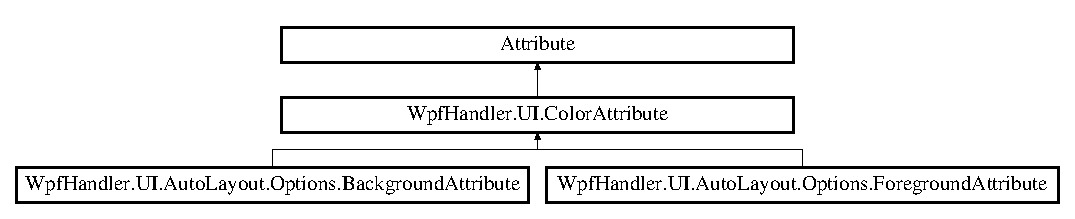
\includegraphics[height=2.500000cm]{d6/dab/class_wpf_handler_1_1_u_i_1_1_color_attribute}
\end{center}
\end{figure}
\subsection*{Public Member Functions}
\begin{DoxyCompactItemize}
\item 
\mbox{\hyperlink{class_wpf_handler_1_1_u_i_1_1_color_attribute_a55398dce3088472e741cfa5682090e4f}{Color\+Attribute}} (\mbox{\hyperlink{class_wpf_handler_1_1_u_i_1_1_color_attribute_afa14c4542d8023b3ddad6aba74993877}{Brush}} brush)
\begin{DoxyCompactList}\small\item\em Instiniating attribute with applied brush. \end{DoxyCompactList}\item 
\mbox{\hyperlink{class_wpf_handler_1_1_u_i_1_1_color_attribute_a5a07f18b18eff772c26e484a764b38f3}{Color\+Attribute}} (Solid\+Color\+Brush brush)
\begin{DoxyCompactList}\small\item\em Instiniating attribute with applied brush. \end{DoxyCompactList}\item 
\mbox{\hyperlink{class_wpf_handler_1_1_u_i_1_1_color_attribute_adc45633c132e90d33ae037b138e31250}{Color\+Attribute}} (string color\+Code)
\begin{DoxyCompactList}\small\item\em Instiniating attribute with applied brush. \end{DoxyCompactList}\item 
\mbox{\hyperlink{class_wpf_handler_1_1_u_i_1_1_color_attribute_a4f6a8ef0ae7f5da318a1c18eafdfbc98}{Color\+Attribute}} (\mbox{\hyperlink{class_wpf_handler_1_1_u_i_1_1_color_attribute_a6c5c2202427bd48877142ecf85327843}{Color}} color)
\begin{DoxyCompactList}\small\item\em Instiniating attribute with applied color. \end{DoxyCompactList}\end{DoxyCompactItemize}
\subsection*{Properties}
\begin{DoxyCompactItemize}
\item 
Color \mbox{\hyperlink{class_wpf_handler_1_1_u_i_1_1_color_attribute_a6c5c2202427bd48877142ecf85327843}{Color}}\hspace{0.3cm}{\ttfamily  \mbox{[}set\mbox{]}}
\begin{DoxyCompactList}\small\item\em Applying color to hte brush. \end{DoxyCompactList}\item 
string \mbox{\hyperlink{class_wpf_handler_1_1_u_i_1_1_color_attribute_a2f09d55a6dfaf3912f2941910e1936e8}{String\+Color}}\hspace{0.3cm}{\ttfamily  \mbox{[}set\mbox{]}}
\begin{DoxyCompactList}\small\item\em Trying to apply string color code as brush by using Color\+Converter rules. Not throw excption in case if color\textquotesingle{}s code invalid to prevent \mbox{\hyperlink{namespace_wpf_handler_1_1_u_i}{UI}} crash. \end{DoxyCompactList}\item 
Brush \mbox{\hyperlink{class_wpf_handler_1_1_u_i_1_1_color_attribute_afa14c4542d8023b3ddad6aba74993877}{Brush}}\hspace{0.3cm}{\ttfamily  \mbox{[}get, set\mbox{]}}
\begin{DoxyCompactList}\small\item\em Brush that will applied to G\+UI element. \end{DoxyCompactList}\end{DoxyCompactItemize}
\subsection*{Private Attributes}
\begin{DoxyCompactItemize}
\item 
\mbox{\hyperlink{class_wpf_handler_1_1_u_i_1_1_color_attribute_afa14c4542d8023b3ddad6aba74993877}{Brush}} \mbox{\hyperlink{class_wpf_handler_1_1_u_i_1_1_color_attribute_ae25cb492c8efb5e3ff570452b618ee23}{\+\_\+\+Brush}}
\begin{DoxyCompactList}\small\item\em Bufer that contains generated or shared Brush. \end{DoxyCompactList}\end{DoxyCompactItemize}


\subsection{Detailed Description}
Base class for color attributes that provides unioform convertion A\+PI for color mamangment relative to the W\+PF. 



\subsection{Constructor \& Destructor Documentation}
\mbox{\Hypertarget{class_wpf_handler_1_1_u_i_1_1_color_attribute_a55398dce3088472e741cfa5682090e4f}\label{class_wpf_handler_1_1_u_i_1_1_color_attribute_a55398dce3088472e741cfa5682090e4f}} 
\index{Wpf\+Handler\+::\+U\+I\+::\+Color\+Attribute@{Wpf\+Handler\+::\+U\+I\+::\+Color\+Attribute}!Color\+Attribute@{Color\+Attribute}}
\index{Color\+Attribute@{Color\+Attribute}!Wpf\+Handler\+::\+U\+I\+::\+Color\+Attribute@{Wpf\+Handler\+::\+U\+I\+::\+Color\+Attribute}}
\subsubsection{\texorpdfstring{Color\+Attribute()}{ColorAttribute()}\hspace{0.1cm}{\footnotesize\ttfamily [1/4]}}
{\footnotesize\ttfamily Wpf\+Handler.\+U\+I.\+Color\+Attribute.\+Color\+Attribute (\begin{DoxyParamCaption}\item[{\mbox{\hyperlink{class_wpf_handler_1_1_u_i_1_1_color_attribute_afa14c4542d8023b3ddad6aba74993877}{Brush}}}]{brush }\end{DoxyParamCaption})}



Instiniating attribute with applied brush. 


\begin{DoxyParams}{Parameters}
{\em brush} & Target brush.\\
\hline
\end{DoxyParams}


No supported via attribute.\mbox{\Hypertarget{class_wpf_handler_1_1_u_i_1_1_color_attribute_a5a07f18b18eff772c26e484a764b38f3}\label{class_wpf_handler_1_1_u_i_1_1_color_attribute_a5a07f18b18eff772c26e484a764b38f3}} 
\index{Wpf\+Handler\+::\+U\+I\+::\+Color\+Attribute@{Wpf\+Handler\+::\+U\+I\+::\+Color\+Attribute}!Color\+Attribute@{Color\+Attribute}}
\index{Color\+Attribute@{Color\+Attribute}!Wpf\+Handler\+::\+U\+I\+::\+Color\+Attribute@{Wpf\+Handler\+::\+U\+I\+::\+Color\+Attribute}}
\subsubsection{\texorpdfstring{Color\+Attribute()}{ColorAttribute()}\hspace{0.1cm}{\footnotesize\ttfamily [2/4]}}
{\footnotesize\ttfamily Wpf\+Handler.\+U\+I.\+Color\+Attribute.\+Color\+Attribute (\begin{DoxyParamCaption}\item[{Solid\+Color\+Brush}]{brush }\end{DoxyParamCaption})}



Instiniating attribute with applied brush. 


\begin{DoxyParams}{Parameters}
{\em brush} & Target brush.\\
\hline
\end{DoxyParams}


No supported via attribute.\mbox{\Hypertarget{class_wpf_handler_1_1_u_i_1_1_color_attribute_adc45633c132e90d33ae037b138e31250}\label{class_wpf_handler_1_1_u_i_1_1_color_attribute_adc45633c132e90d33ae037b138e31250}} 
\index{Wpf\+Handler\+::\+U\+I\+::\+Color\+Attribute@{Wpf\+Handler\+::\+U\+I\+::\+Color\+Attribute}!Color\+Attribute@{Color\+Attribute}}
\index{Color\+Attribute@{Color\+Attribute}!Wpf\+Handler\+::\+U\+I\+::\+Color\+Attribute@{Wpf\+Handler\+::\+U\+I\+::\+Color\+Attribute}}
\subsubsection{\texorpdfstring{Color\+Attribute()}{ColorAttribute()}\hspace{0.1cm}{\footnotesize\ttfamily [3/4]}}
{\footnotesize\ttfamily Wpf\+Handler.\+U\+I.\+Color\+Attribute.\+Color\+Attribute (\begin{DoxyParamCaption}\item[{string}]{color\+Code }\end{DoxyParamCaption})}



Instiniating attribute with applied brush. 


\begin{DoxyParams}{Parameters}
{\em color\+Code} & Trying to apply string color code as brush by using Color\+Converter rules. Not throw excption in case if color\textquotesingle{}s code invalid to prevent \mbox{\hyperlink{namespace_wpf_handler_1_1_u_i}{UI}} crash.\\
\hline
\end{DoxyParams}
\mbox{\Hypertarget{class_wpf_handler_1_1_u_i_1_1_color_attribute_a4f6a8ef0ae7f5da318a1c18eafdfbc98}\label{class_wpf_handler_1_1_u_i_1_1_color_attribute_a4f6a8ef0ae7f5da318a1c18eafdfbc98}} 
\index{Wpf\+Handler\+::\+U\+I\+::\+Color\+Attribute@{Wpf\+Handler\+::\+U\+I\+::\+Color\+Attribute}!Color\+Attribute@{Color\+Attribute}}
\index{Color\+Attribute@{Color\+Attribute}!Wpf\+Handler\+::\+U\+I\+::\+Color\+Attribute@{Wpf\+Handler\+::\+U\+I\+::\+Color\+Attribute}}
\subsubsection{\texorpdfstring{Color\+Attribute()}{ColorAttribute()}\hspace{0.1cm}{\footnotesize\ttfamily [4/4]}}
{\footnotesize\ttfamily Wpf\+Handler.\+U\+I.\+Color\+Attribute.\+Color\+Attribute (\begin{DoxyParamCaption}\item[{\mbox{\hyperlink{class_wpf_handler_1_1_u_i_1_1_color_attribute_a6c5c2202427bd48877142ecf85327843}{Color}}}]{color }\end{DoxyParamCaption})}



Instiniating attribute with applied color. 


\begin{DoxyParams}{Parameters}
{\em color} & Target color.\\
\hline
\end{DoxyParams}


No supported via attribute.

\subsection{Member Data Documentation}
\mbox{\Hypertarget{class_wpf_handler_1_1_u_i_1_1_color_attribute_ae25cb492c8efb5e3ff570452b618ee23}\label{class_wpf_handler_1_1_u_i_1_1_color_attribute_ae25cb492c8efb5e3ff570452b618ee23}} 
\index{Wpf\+Handler\+::\+U\+I\+::\+Color\+Attribute@{Wpf\+Handler\+::\+U\+I\+::\+Color\+Attribute}!\+\_\+\+Brush@{\+\_\+\+Brush}}
\index{\+\_\+\+Brush@{\+\_\+\+Brush}!Wpf\+Handler\+::\+U\+I\+::\+Color\+Attribute@{Wpf\+Handler\+::\+U\+I\+::\+Color\+Attribute}}
\subsubsection{\texorpdfstring{\+\_\+\+Brush}{\_Brush}}
{\footnotesize\ttfamily \mbox{\hyperlink{class_wpf_handler_1_1_u_i_1_1_color_attribute_afa14c4542d8023b3ddad6aba74993877}{Brush}} Wpf\+Handler.\+U\+I.\+Color\+Attribute.\+\_\+\+Brush\hspace{0.3cm}{\ttfamily [private]}}



Bufer that contains generated or shared Brush. 



\subsection{Property Documentation}
\mbox{\Hypertarget{class_wpf_handler_1_1_u_i_1_1_color_attribute_afa14c4542d8023b3ddad6aba74993877}\label{class_wpf_handler_1_1_u_i_1_1_color_attribute_afa14c4542d8023b3ddad6aba74993877}} 
\index{Wpf\+Handler\+::\+U\+I\+::\+Color\+Attribute@{Wpf\+Handler\+::\+U\+I\+::\+Color\+Attribute}!Brush@{Brush}}
\index{Brush@{Brush}!Wpf\+Handler\+::\+U\+I\+::\+Color\+Attribute@{Wpf\+Handler\+::\+U\+I\+::\+Color\+Attribute}}
\subsubsection{\texorpdfstring{Brush}{Brush}}
{\footnotesize\ttfamily Brush Wpf\+Handler.\+U\+I.\+Color\+Attribute.\+Brush\hspace{0.3cm}{\ttfamily [get]}, {\ttfamily [set]}}



Brush that will applied to G\+UI element. 

\mbox{\Hypertarget{class_wpf_handler_1_1_u_i_1_1_color_attribute_a6c5c2202427bd48877142ecf85327843}\label{class_wpf_handler_1_1_u_i_1_1_color_attribute_a6c5c2202427bd48877142ecf85327843}} 
\index{Wpf\+Handler\+::\+U\+I\+::\+Color\+Attribute@{Wpf\+Handler\+::\+U\+I\+::\+Color\+Attribute}!Color@{Color}}
\index{Color@{Color}!Wpf\+Handler\+::\+U\+I\+::\+Color\+Attribute@{Wpf\+Handler\+::\+U\+I\+::\+Color\+Attribute}}
\subsubsection{\texorpdfstring{Color}{Color}}
{\footnotesize\ttfamily Color Wpf\+Handler.\+U\+I.\+Color\+Attribute.\+Color\hspace{0.3cm}{\ttfamily [set]}}



Applying color to hte brush. 

\mbox{\Hypertarget{class_wpf_handler_1_1_u_i_1_1_color_attribute_a2f09d55a6dfaf3912f2941910e1936e8}\label{class_wpf_handler_1_1_u_i_1_1_color_attribute_a2f09d55a6dfaf3912f2941910e1936e8}} 
\index{Wpf\+Handler\+::\+U\+I\+::\+Color\+Attribute@{Wpf\+Handler\+::\+U\+I\+::\+Color\+Attribute}!String\+Color@{String\+Color}}
\index{String\+Color@{String\+Color}!Wpf\+Handler\+::\+U\+I\+::\+Color\+Attribute@{Wpf\+Handler\+::\+U\+I\+::\+Color\+Attribute}}
\subsubsection{\texorpdfstring{String\+Color}{StringColor}}
{\footnotesize\ttfamily string Wpf\+Handler.\+U\+I.\+Color\+Attribute.\+String\+Color\hspace{0.3cm}{\ttfamily [set]}}



Trying to apply string color code as brush by using Color\+Converter rules. Not throw excption in case if color\textquotesingle{}s code invalid to prevent \mbox{\hyperlink{namespace_wpf_handler_1_1_u_i}{UI}} crash. 



The documentation for this class was generated from the following file\+:\begin{DoxyCompactItemize}
\item 
D\+:/\+Work/\+Git\+Hub/wpf-\/handler/\+Wpf\+Handler/\+U\+I/Color\+Attribute.\+cs\end{DoxyCompactItemize}

\hypertarget{class_wpf_handler_1_1_plugins_1_1_constants}{}\section{Wpf\+Handler.\+Plugins.\+Constants Class Reference}
\label{class_wpf_handler_1_1_plugins_1_1_constants}\index{Wpf\+Handler.\+Plugins.\+Constants@{Wpf\+Handler.\+Plugins.\+Constants}}
\subsection*{Public Attributes}
\begin{DoxyCompactItemize}
\item 
const string \mbox{\hyperlink{class_wpf_handler_1_1_plugins_1_1_constants_a96f55ef86fe92a534722f4788340f390}{P\+L\+U\+G\+I\+N\+S\+\_\+\+D\+IR}} = \char`\"{}plugins/\char`\"{}
\begin{DoxyCompactList}\small\item\em Relative directory with plugins. \end{DoxyCompactList}\item 
const string \mbox{\hyperlink{class_wpf_handler_1_1_plugins_1_1_constants_aa7969fd3e77b585b42f0c99a5440dbb2}{T\+H\+E\+M\+E\+S\+\_\+\+D\+IR}} = \char`\"{}plugins/themes/\char`\"{}
\begin{DoxyCompactList}\small\item\em Relative directory with themes xaml files. \end{DoxyCompactList}\end{DoxyCompactItemize}


\subsection{Member Data Documentation}
\mbox{\Hypertarget{class_wpf_handler_1_1_plugins_1_1_constants_a96f55ef86fe92a534722f4788340f390}\label{class_wpf_handler_1_1_plugins_1_1_constants_a96f55ef86fe92a534722f4788340f390}} 
\index{Wpf\+Handler\+::\+Plugins\+::\+Constants@{Wpf\+Handler\+::\+Plugins\+::\+Constants}!P\+L\+U\+G\+I\+N\+S\+\_\+\+D\+IR@{P\+L\+U\+G\+I\+N\+S\+\_\+\+D\+IR}}
\index{P\+L\+U\+G\+I\+N\+S\+\_\+\+D\+IR@{P\+L\+U\+G\+I\+N\+S\+\_\+\+D\+IR}!Wpf\+Handler\+::\+Plugins\+::\+Constants@{Wpf\+Handler\+::\+Plugins\+::\+Constants}}
\subsubsection{\texorpdfstring{P\+L\+U\+G\+I\+N\+S\+\_\+\+D\+IR}{PLUGINS\_DIR}}
{\footnotesize\ttfamily const string Wpf\+Handler.\+Plugins.\+Constants.\+P\+L\+U\+G\+I\+N\+S\+\_\+\+D\+IR = \char`\"{}plugins/\char`\"{}}



Relative directory with plugins. 

\mbox{\Hypertarget{class_wpf_handler_1_1_plugins_1_1_constants_aa7969fd3e77b585b42f0c99a5440dbb2}\label{class_wpf_handler_1_1_plugins_1_1_constants_aa7969fd3e77b585b42f0c99a5440dbb2}} 
\index{Wpf\+Handler\+::\+Plugins\+::\+Constants@{Wpf\+Handler\+::\+Plugins\+::\+Constants}!T\+H\+E\+M\+E\+S\+\_\+\+D\+IR@{T\+H\+E\+M\+E\+S\+\_\+\+D\+IR}}
\index{T\+H\+E\+M\+E\+S\+\_\+\+D\+IR@{T\+H\+E\+M\+E\+S\+\_\+\+D\+IR}!Wpf\+Handler\+::\+Plugins\+::\+Constants@{Wpf\+Handler\+::\+Plugins\+::\+Constants}}
\subsubsection{\texorpdfstring{T\+H\+E\+M\+E\+S\+\_\+\+D\+IR}{THEMES\_DIR}}
{\footnotesize\ttfamily const string Wpf\+Handler.\+Plugins.\+Constants.\+T\+H\+E\+M\+E\+S\+\_\+\+D\+IR = \char`\"{}plugins/themes/\char`\"{}}



Relative directory with themes xaml files. 



The documentation for this class was generated from the following file\+:\begin{DoxyCompactItemize}
\item 
D\+:/\+Work/\+Git\+Hub/wpf-\/handler/\+Wpf\+Handler/\+Plugins/Constants.\+cs\end{DoxyCompactItemize}

\hypertarget{class_wpf_handler_1_1_u_i_1_1_auto_layout_1_1_configuration_1_1_content_attribute}{}\section{Wpf\+Handler.\+U\+I.\+Auto\+Layout.\+Configuration.\+Content\+Attribute Class Reference}
\label{class_wpf_handler_1_1_u_i_1_1_auto_layout_1_1_configuration_1_1_content_attribute}\index{Wpf\+Handler.\+U\+I.\+Auto\+Layout.\+Configuration.\+Content\+Attribute@{Wpf\+Handler.\+U\+I.\+Auto\+Layout.\+Configuration.\+Content\+Attribute}}


Defines a \mbox{\hyperlink{class_wpf_handler_1_1_u_i_1_1_g_u_i_content}{G\+U\+I\+Content}} applied to the member.  


Inheritance diagram for Wpf\+Handler.\+U\+I.\+Auto\+Layout.\+Configuration.\+Content\+Attribute\+:\begin{figure}[H]
\begin{center}
\leavevmode
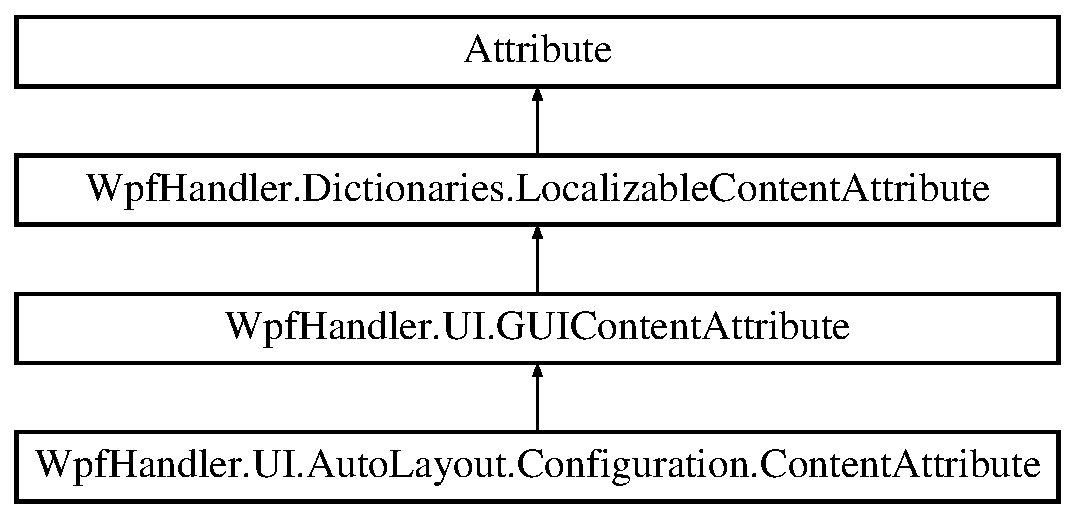
\includegraphics[height=4.000000cm]{d2/dfc/class_wpf_handler_1_1_u_i_1_1_auto_layout_1_1_configuration_1_1_content_attribute}
\end{center}
\end{figure}
\subsection*{Public Member Functions}
\begin{DoxyCompactItemize}
\item 
\mbox{\hyperlink{class_wpf_handler_1_1_u_i_1_1_auto_layout_1_1_configuration_1_1_content_attribute_acdfac4309551dd388a4f039b9e9263dc}{Content\+Attribute}} ()
\begin{DoxyCompactList}\small\item\em Instiniate new atribute with null G\+UI content. \end{DoxyCompactList}\item 
\mbox{\hyperlink{class_wpf_handler_1_1_u_i_1_1_auto_layout_1_1_configuration_1_1_content_attribute_ac65e5b234d917c37a95b5471ef8b41b0}{Content\+Attribute}} (string title)
\begin{DoxyCompactList}\small\item\em Auto initialize content with shared title value. \end{DoxyCompactList}\item 
\mbox{\hyperlink{class_wpf_handler_1_1_u_i_1_1_auto_layout_1_1_configuration_1_1_content_attribute_ac44c492fbdc06f7a28f77c4dcb50e828}{Content\+Attribute}} (string title, string description)
\begin{DoxyCompactList}\small\item\em Constructor that allow to set title. \end{DoxyCompactList}\item 
\mbox{\hyperlink{class_wpf_handler_1_1_u_i_1_1_auto_layout_1_1_configuration_1_1_content_attribute_ab0c84b73301dd184abc00bbf5204c178}{Content\+Attribute}} (string default\+Title, string default\+Description, string decription\+Localization\+Resourse\+Key)
\begin{DoxyCompactList}\small\item\em Initialize all allowed fields. \end{DoxyCompactList}\item 
\mbox{\hyperlink{class_wpf_handler_1_1_u_i_1_1_auto_layout_1_1_configuration_1_1_content_attribute_a54c8ed64b08dbbf380bfb47cbe2829e2}{Content\+Attribute}} (string default\+Title, string default\+Description, string title\+Localization\+Resourse\+Key, string decription\+Localization\+Resourse\+Key)
\begin{DoxyCompactList}\small\item\em Initialize all allowed fields. \end{DoxyCompactList}\item 
override void \mbox{\hyperlink{class_wpf_handler_1_1_u_i_1_1_auto_layout_1_1_configuration_1_1_content_attribute_a498818bc121b7f408af302eb4085056a}{Languages\+Dictionaries\+Updated}} ()
\begin{DoxyCompactList}\small\item\em Callback that will occurs in case of updating of the language dictionaries. \end{DoxyCompactList}\item 
void \mbox{\hyperlink{class_wpf_handler_1_1_u_i_1_1_auto_layout_1_1_configuration_1_1_content_attribute_a0d0f48fc255493eec2f341b9b90d5eee}{Bind\+To\+Label}} (\mbox{\hyperlink{interface_wpf_handler_1_1_u_i_1_1_controls_1_1_i_label}{I\+Label}} label)
\begin{DoxyCompactList}\small\item\em Connecting instiniated control with label to localization updates. \end{DoxyCompactList}\item 
void \mbox{\hyperlink{class_wpf_handler_1_1_u_i_1_1_auto_layout_1_1_configuration_1_1_content_attribute_aced8f451c4ff60a54694d64581432a36}{Bind\+To\+Label}} (\mbox{\hyperlink{interface_wpf_handler_1_1_u_i_1_1_controls_1_1_i_label}{I\+Label}} label, Member\+Info source\+Member)
\begin{DoxyCompactList}\small\item\em Connecting instiniated control with label to localization updates. \end{DoxyCompactList}\end{DoxyCompactItemize}
\subsection*{Properties}
\begin{DoxyCompactItemize}
\item 
static \mbox{\hyperlink{class_wpf_handler_1_1_u_i_1_1_auto_layout_1_1_configuration_1_1_content_attribute}{Content\+Attribute}} \mbox{\hyperlink{class_wpf_handler_1_1_u_i_1_1_auto_layout_1_1_configuration_1_1_content_attribute_a7342c312b16ecde3884a20ae56879485}{Empty}}\hspace{0.3cm}{\ttfamily  \mbox{[}get\mbox{]}}
\begin{DoxyCompactList}\small\item\em Return new attribute instance with None content. \end{DoxyCompactList}\item 
\mbox{\hyperlink{interface_wpf_handler_1_1_u_i_1_1_controls_1_1_i_label}{I\+Label}} \mbox{\hyperlink{class_wpf_handler_1_1_u_i_1_1_auto_layout_1_1_configuration_1_1_content_attribute_a27ac4fe8d5fdf953c624a099b7c33ac4}{Binded\+Label}}\hspace{0.3cm}{\ttfamily  \mbox{[}get, protected set\mbox{]}}
\begin{DoxyCompactList}\small\item\em Instiniated control with a label. \end{DoxyCompactList}\item 
Member\+Info \mbox{\hyperlink{class_wpf_handler_1_1_u_i_1_1_auto_layout_1_1_configuration_1_1_content_attribute_ac04878f4eb3c6ceb3c3f5c726fc34d50}{Binded\+Member}}\hspace{0.3cm}{\ttfamily  \mbox{[}get, protected set\mbox{]}}
\begin{DoxyCompactList}\small\item\em Member info that will be used to auto generation of the field\textquotesingle{}s label content. \end{DoxyCompactList}\end{DoxyCompactItemize}


\subsection{Detailed Description}
Defines a \mbox{\hyperlink{class_wpf_handler_1_1_u_i_1_1_g_u_i_content}{G\+U\+I\+Content}} applied to the member. 



\subsection{Constructor \& Destructor Documentation}
\mbox{\Hypertarget{class_wpf_handler_1_1_u_i_1_1_auto_layout_1_1_configuration_1_1_content_attribute_acdfac4309551dd388a4f039b9e9263dc}\label{class_wpf_handler_1_1_u_i_1_1_auto_layout_1_1_configuration_1_1_content_attribute_acdfac4309551dd388a4f039b9e9263dc}} 
\index{Wpf\+Handler\+::\+U\+I\+::\+Auto\+Layout\+::\+Configuration\+::\+Content\+Attribute@{Wpf\+Handler\+::\+U\+I\+::\+Auto\+Layout\+::\+Configuration\+::\+Content\+Attribute}!Content\+Attribute@{Content\+Attribute}}
\index{Content\+Attribute@{Content\+Attribute}!Wpf\+Handler\+::\+U\+I\+::\+Auto\+Layout\+::\+Configuration\+::\+Content\+Attribute@{Wpf\+Handler\+::\+U\+I\+::\+Auto\+Layout\+::\+Configuration\+::\+Content\+Attribute}}
\subsubsection{\texorpdfstring{Content\+Attribute()}{ContentAttribute()}\hspace{0.1cm}{\footnotesize\ttfamily [1/5]}}
{\footnotesize\ttfamily Wpf\+Handler.\+U\+I.\+Auto\+Layout.\+Configuration.\+Content\+Attribute.\+Content\+Attribute (\begin{DoxyParamCaption}{ }\end{DoxyParamCaption})}



Instiniate new atribute with null G\+UI content. 

\mbox{\Hypertarget{class_wpf_handler_1_1_u_i_1_1_auto_layout_1_1_configuration_1_1_content_attribute_ac65e5b234d917c37a95b5471ef8b41b0}\label{class_wpf_handler_1_1_u_i_1_1_auto_layout_1_1_configuration_1_1_content_attribute_ac65e5b234d917c37a95b5471ef8b41b0}} 
\index{Wpf\+Handler\+::\+U\+I\+::\+Auto\+Layout\+::\+Configuration\+::\+Content\+Attribute@{Wpf\+Handler\+::\+U\+I\+::\+Auto\+Layout\+::\+Configuration\+::\+Content\+Attribute}!Content\+Attribute@{Content\+Attribute}}
\index{Content\+Attribute@{Content\+Attribute}!Wpf\+Handler\+::\+U\+I\+::\+Auto\+Layout\+::\+Configuration\+::\+Content\+Attribute@{Wpf\+Handler\+::\+U\+I\+::\+Auto\+Layout\+::\+Configuration\+::\+Content\+Attribute}}
\subsubsection{\texorpdfstring{Content\+Attribute()}{ContentAttribute()}\hspace{0.1cm}{\footnotesize\ttfamily [2/5]}}
{\footnotesize\ttfamily Wpf\+Handler.\+U\+I.\+Auto\+Layout.\+Configuration.\+Content\+Attribute.\+Content\+Attribute (\begin{DoxyParamCaption}\item[{string}]{title }\end{DoxyParamCaption})}



Auto initialize content with shared title value. 


\begin{DoxyParams}{Parameters}
{\em title} & Title that will be showed up into the label.\\
\hline
\end{DoxyParams}
\mbox{\Hypertarget{class_wpf_handler_1_1_u_i_1_1_auto_layout_1_1_configuration_1_1_content_attribute_ac44c492fbdc06f7a28f77c4dcb50e828}\label{class_wpf_handler_1_1_u_i_1_1_auto_layout_1_1_configuration_1_1_content_attribute_ac44c492fbdc06f7a28f77c4dcb50e828}} 
\index{Wpf\+Handler\+::\+U\+I\+::\+Auto\+Layout\+::\+Configuration\+::\+Content\+Attribute@{Wpf\+Handler\+::\+U\+I\+::\+Auto\+Layout\+::\+Configuration\+::\+Content\+Attribute}!Content\+Attribute@{Content\+Attribute}}
\index{Content\+Attribute@{Content\+Attribute}!Wpf\+Handler\+::\+U\+I\+::\+Auto\+Layout\+::\+Configuration\+::\+Content\+Attribute@{Wpf\+Handler\+::\+U\+I\+::\+Auto\+Layout\+::\+Configuration\+::\+Content\+Attribute}}
\subsubsection{\texorpdfstring{Content\+Attribute()}{ContentAttribute()}\hspace{0.1cm}{\footnotesize\ttfamily [3/5]}}
{\footnotesize\ttfamily Wpf\+Handler.\+U\+I.\+Auto\+Layout.\+Configuration.\+Content\+Attribute.\+Content\+Attribute (\begin{DoxyParamCaption}\item[{string}]{title,  }\item[{string}]{description }\end{DoxyParamCaption})}



Constructor that allow to set title. 


\begin{DoxyParams}{Parameters}
{\em title} & Title of that element.\\
\hline
{\em description} & Description of that element.\\
\hline
\end{DoxyParams}
\mbox{\Hypertarget{class_wpf_handler_1_1_u_i_1_1_auto_layout_1_1_configuration_1_1_content_attribute_ab0c84b73301dd184abc00bbf5204c178}\label{class_wpf_handler_1_1_u_i_1_1_auto_layout_1_1_configuration_1_1_content_attribute_ab0c84b73301dd184abc00bbf5204c178}} 
\index{Wpf\+Handler\+::\+U\+I\+::\+Auto\+Layout\+::\+Configuration\+::\+Content\+Attribute@{Wpf\+Handler\+::\+U\+I\+::\+Auto\+Layout\+::\+Configuration\+::\+Content\+Attribute}!Content\+Attribute@{Content\+Attribute}}
\index{Content\+Attribute@{Content\+Attribute}!Wpf\+Handler\+::\+U\+I\+::\+Auto\+Layout\+::\+Configuration\+::\+Content\+Attribute@{Wpf\+Handler\+::\+U\+I\+::\+Auto\+Layout\+::\+Configuration\+::\+Content\+Attribute}}
\subsubsection{\texorpdfstring{Content\+Attribute()}{ContentAttribute()}\hspace{0.1cm}{\footnotesize\ttfamily [4/5]}}
{\footnotesize\ttfamily Wpf\+Handler.\+U\+I.\+Auto\+Layout.\+Configuration.\+Content\+Attribute.\+Content\+Attribute (\begin{DoxyParamCaption}\item[{string}]{default\+Title,  }\item[{string}]{default\+Description,  }\item[{string}]{decription\+Localization\+Resourse\+Key }\end{DoxyParamCaption})}



Initialize all allowed fields. 


\begin{DoxyParams}{Parameters}
{\em default\+Title} & Title that would be used by default if localization dictionary not found.\\
\hline
{\em default\+Description} & Default description if localization dictionary not found.\\
\hline
{\em decription\+Localization\+Resourse\+Key} & Key of description content in localized dynamic dictionary.\\
\hline
\end{DoxyParams}
\mbox{\Hypertarget{class_wpf_handler_1_1_u_i_1_1_auto_layout_1_1_configuration_1_1_content_attribute_a54c8ed64b08dbbf380bfb47cbe2829e2}\label{class_wpf_handler_1_1_u_i_1_1_auto_layout_1_1_configuration_1_1_content_attribute_a54c8ed64b08dbbf380bfb47cbe2829e2}} 
\index{Wpf\+Handler\+::\+U\+I\+::\+Auto\+Layout\+::\+Configuration\+::\+Content\+Attribute@{Wpf\+Handler\+::\+U\+I\+::\+Auto\+Layout\+::\+Configuration\+::\+Content\+Attribute}!Content\+Attribute@{Content\+Attribute}}
\index{Content\+Attribute@{Content\+Attribute}!Wpf\+Handler\+::\+U\+I\+::\+Auto\+Layout\+::\+Configuration\+::\+Content\+Attribute@{Wpf\+Handler\+::\+U\+I\+::\+Auto\+Layout\+::\+Configuration\+::\+Content\+Attribute}}
\subsubsection{\texorpdfstring{Content\+Attribute()}{ContentAttribute()}\hspace{0.1cm}{\footnotesize\ttfamily [5/5]}}
{\footnotesize\ttfamily Wpf\+Handler.\+U\+I.\+Auto\+Layout.\+Configuration.\+Content\+Attribute.\+Content\+Attribute (\begin{DoxyParamCaption}\item[{string}]{default\+Title,  }\item[{string}]{default\+Description,  }\item[{string}]{title\+Localization\+Resourse\+Key,  }\item[{string}]{decription\+Localization\+Resourse\+Key }\end{DoxyParamCaption})}



Initialize all allowed fields. 


\begin{DoxyParams}{Parameters}
{\em default\+Title} & Title that would be used by default if localization dictionary not found.\\
\hline
{\em default\+Description} & Default description if localization dictionary not found.\\
\hline
{\em title\+Localization\+Resourse\+Key} & Key of title content in localized dynamic dictionary.\\
\hline
{\em decription\+Localization\+Resourse\+Key} & Key of description content in localized dynamic dictionary.\\
\hline
\end{DoxyParams}


\subsection{Member Function Documentation}
\mbox{\Hypertarget{class_wpf_handler_1_1_u_i_1_1_auto_layout_1_1_configuration_1_1_content_attribute_a0d0f48fc255493eec2f341b9b90d5eee}\label{class_wpf_handler_1_1_u_i_1_1_auto_layout_1_1_configuration_1_1_content_attribute_a0d0f48fc255493eec2f341b9b90d5eee}} 
\index{Wpf\+Handler\+::\+U\+I\+::\+Auto\+Layout\+::\+Configuration\+::\+Content\+Attribute@{Wpf\+Handler\+::\+U\+I\+::\+Auto\+Layout\+::\+Configuration\+::\+Content\+Attribute}!Bind\+To\+Label@{Bind\+To\+Label}}
\index{Bind\+To\+Label@{Bind\+To\+Label}!Wpf\+Handler\+::\+U\+I\+::\+Auto\+Layout\+::\+Configuration\+::\+Content\+Attribute@{Wpf\+Handler\+::\+U\+I\+::\+Auto\+Layout\+::\+Configuration\+::\+Content\+Attribute}}
\subsubsection{\texorpdfstring{Bind\+To\+Label()}{BindToLabel()}\hspace{0.1cm}{\footnotesize\ttfamily [1/2]}}
{\footnotesize\ttfamily void Wpf\+Handler.\+U\+I.\+Auto\+Layout.\+Configuration.\+Content\+Attribute.\+Bind\+To\+Label (\begin{DoxyParamCaption}\item[{\mbox{\hyperlink{interface_wpf_handler_1_1_u_i_1_1_controls_1_1_i_label}{I\+Label}}}]{label }\end{DoxyParamCaption})}



Connecting instiniated control with label to localization updates. 


\begin{DoxyParams}{Parameters}
{\em label} & \mbox{\hyperlink{namespace_wpf_handler_1_1_u_i}{UI}} control that has a label to content bridging.\\
\hline
\end{DoxyParams}
\mbox{\Hypertarget{class_wpf_handler_1_1_u_i_1_1_auto_layout_1_1_configuration_1_1_content_attribute_aced8f451c4ff60a54694d64581432a36}\label{class_wpf_handler_1_1_u_i_1_1_auto_layout_1_1_configuration_1_1_content_attribute_aced8f451c4ff60a54694d64581432a36}} 
\index{Wpf\+Handler\+::\+U\+I\+::\+Auto\+Layout\+::\+Configuration\+::\+Content\+Attribute@{Wpf\+Handler\+::\+U\+I\+::\+Auto\+Layout\+::\+Configuration\+::\+Content\+Attribute}!Bind\+To\+Label@{Bind\+To\+Label}}
\index{Bind\+To\+Label@{Bind\+To\+Label}!Wpf\+Handler\+::\+U\+I\+::\+Auto\+Layout\+::\+Configuration\+::\+Content\+Attribute@{Wpf\+Handler\+::\+U\+I\+::\+Auto\+Layout\+::\+Configuration\+::\+Content\+Attribute}}
\subsubsection{\texorpdfstring{Bind\+To\+Label()}{BindToLabel()}\hspace{0.1cm}{\footnotesize\ttfamily [2/2]}}
{\footnotesize\ttfamily void Wpf\+Handler.\+U\+I.\+Auto\+Layout.\+Configuration.\+Content\+Attribute.\+Bind\+To\+Label (\begin{DoxyParamCaption}\item[{\mbox{\hyperlink{interface_wpf_handler_1_1_u_i_1_1_controls_1_1_i_label}{I\+Label}}}]{label,  }\item[{Member\+Info}]{source\+Member }\end{DoxyParamCaption})}



Connecting instiniated control with label to localization updates. 


\begin{DoxyParams}{Parameters}
{\em label} & \mbox{\hyperlink{namespace_wpf_handler_1_1_u_i}{UI}} control that has a label to content bridging.\\
\hline
{\em source\+Member} & Member infor that could be used as source for auto generated title in case if \mbox{\hyperlink{class_wpf_handler_1_1_u_i_1_1_g_u_i_content}{G\+U\+I\+Content}} not provided in resources.\\
\hline
\end{DoxyParams}
\mbox{\Hypertarget{class_wpf_handler_1_1_u_i_1_1_auto_layout_1_1_configuration_1_1_content_attribute_a498818bc121b7f408af302eb4085056a}\label{class_wpf_handler_1_1_u_i_1_1_auto_layout_1_1_configuration_1_1_content_attribute_a498818bc121b7f408af302eb4085056a}} 
\index{Wpf\+Handler\+::\+U\+I\+::\+Auto\+Layout\+::\+Configuration\+::\+Content\+Attribute@{Wpf\+Handler\+::\+U\+I\+::\+Auto\+Layout\+::\+Configuration\+::\+Content\+Attribute}!Languages\+Dictionaries\+Updated@{Languages\+Dictionaries\+Updated}}
\index{Languages\+Dictionaries\+Updated@{Languages\+Dictionaries\+Updated}!Wpf\+Handler\+::\+U\+I\+::\+Auto\+Layout\+::\+Configuration\+::\+Content\+Attribute@{Wpf\+Handler\+::\+U\+I\+::\+Auto\+Layout\+::\+Configuration\+::\+Content\+Attribute}}
\subsubsection{\texorpdfstring{Languages\+Dictionaries\+Updated()}{LanguagesDictionariesUpdated()}}
{\footnotesize\ttfamily override void Wpf\+Handler.\+U\+I.\+Auto\+Layout.\+Configuration.\+Content\+Attribute.\+Languages\+Dictionaries\+Updated (\begin{DoxyParamCaption}{ }\end{DoxyParamCaption})\hspace{0.3cm}{\ttfamily [virtual]}}



Callback that will occurs in case of updating of the language dictionaries. 



Implements \mbox{\hyperlink{class_wpf_handler_1_1_dictionaries_1_1_localizable_content_attribute_a001e110c7ad42422bc02a44d9eedc801}{Wpf\+Handler.\+Dictionaries.\+Localizable\+Content\+Attribute}}.



\subsection{Property Documentation}
\mbox{\Hypertarget{class_wpf_handler_1_1_u_i_1_1_auto_layout_1_1_configuration_1_1_content_attribute_a27ac4fe8d5fdf953c624a099b7c33ac4}\label{class_wpf_handler_1_1_u_i_1_1_auto_layout_1_1_configuration_1_1_content_attribute_a27ac4fe8d5fdf953c624a099b7c33ac4}} 
\index{Wpf\+Handler\+::\+U\+I\+::\+Auto\+Layout\+::\+Configuration\+::\+Content\+Attribute@{Wpf\+Handler\+::\+U\+I\+::\+Auto\+Layout\+::\+Configuration\+::\+Content\+Attribute}!Binded\+Label@{Binded\+Label}}
\index{Binded\+Label@{Binded\+Label}!Wpf\+Handler\+::\+U\+I\+::\+Auto\+Layout\+::\+Configuration\+::\+Content\+Attribute@{Wpf\+Handler\+::\+U\+I\+::\+Auto\+Layout\+::\+Configuration\+::\+Content\+Attribute}}
\subsubsection{\texorpdfstring{Binded\+Label}{BindedLabel}}
{\footnotesize\ttfamily \mbox{\hyperlink{interface_wpf_handler_1_1_u_i_1_1_controls_1_1_i_label}{I\+Label}} Wpf\+Handler.\+U\+I.\+Auto\+Layout.\+Configuration.\+Content\+Attribute.\+Binded\+Label\hspace{0.3cm}{\ttfamily [get]}, {\ttfamily [protected set]}}



Instiniated control with a label. 

\mbox{\Hypertarget{class_wpf_handler_1_1_u_i_1_1_auto_layout_1_1_configuration_1_1_content_attribute_ac04878f4eb3c6ceb3c3f5c726fc34d50}\label{class_wpf_handler_1_1_u_i_1_1_auto_layout_1_1_configuration_1_1_content_attribute_ac04878f4eb3c6ceb3c3f5c726fc34d50}} 
\index{Wpf\+Handler\+::\+U\+I\+::\+Auto\+Layout\+::\+Configuration\+::\+Content\+Attribute@{Wpf\+Handler\+::\+U\+I\+::\+Auto\+Layout\+::\+Configuration\+::\+Content\+Attribute}!Binded\+Member@{Binded\+Member}}
\index{Binded\+Member@{Binded\+Member}!Wpf\+Handler\+::\+U\+I\+::\+Auto\+Layout\+::\+Configuration\+::\+Content\+Attribute@{Wpf\+Handler\+::\+U\+I\+::\+Auto\+Layout\+::\+Configuration\+::\+Content\+Attribute}}
\subsubsection{\texorpdfstring{Binded\+Member}{BindedMember}}
{\footnotesize\ttfamily Member\+Info Wpf\+Handler.\+U\+I.\+Auto\+Layout.\+Configuration.\+Content\+Attribute.\+Binded\+Member\hspace{0.3cm}{\ttfamily [get]}, {\ttfamily [protected set]}}



Member info that will be used to auto generation of the field\textquotesingle{}s label content. 

\mbox{\Hypertarget{class_wpf_handler_1_1_u_i_1_1_auto_layout_1_1_configuration_1_1_content_attribute_a7342c312b16ecde3884a20ae56879485}\label{class_wpf_handler_1_1_u_i_1_1_auto_layout_1_1_configuration_1_1_content_attribute_a7342c312b16ecde3884a20ae56879485}} 
\index{Wpf\+Handler\+::\+U\+I\+::\+Auto\+Layout\+::\+Configuration\+::\+Content\+Attribute@{Wpf\+Handler\+::\+U\+I\+::\+Auto\+Layout\+::\+Configuration\+::\+Content\+Attribute}!Empty@{Empty}}
\index{Empty@{Empty}!Wpf\+Handler\+::\+U\+I\+::\+Auto\+Layout\+::\+Configuration\+::\+Content\+Attribute@{Wpf\+Handler\+::\+U\+I\+::\+Auto\+Layout\+::\+Configuration\+::\+Content\+Attribute}}
\subsubsection{\texorpdfstring{Empty}{Empty}}
{\footnotesize\ttfamily \mbox{\hyperlink{class_wpf_handler_1_1_u_i_1_1_auto_layout_1_1_configuration_1_1_content_attribute}{Content\+Attribute}} Wpf\+Handler.\+U\+I.\+Auto\+Layout.\+Configuration.\+Content\+Attribute.\+Empty\hspace{0.3cm}{\ttfamily [static]}, {\ttfamily [get]}}



Return new attribute instance with None content. 



The documentation for this class was generated from the following file\+:\begin{DoxyCompactItemize}
\item 
D\+:/\+Work/\+Git\+Hub/wpf-\/handler/\+Wpf\+Handler/\+U\+I/\+Auto\+Layout/\+Configuration/Content\+Attribute.\+cs\end{DoxyCompactItemize}

\hypertarget{class_wpf_handler_1_1_u_i_1_1_auto_layout_1_1_configuration_1_1_custom_control_attribute}{}\section{Wpf\+Handler.\+U\+I.\+Auto\+Layout.\+Configuration.\+Custom\+Control\+Attribute Class Reference}
\label{class_wpf_handler_1_1_u_i_1_1_auto_layout_1_1_configuration_1_1_custom_control_attribute}\index{Wpf\+Handler.\+U\+I.\+Auto\+Layout.\+Configuration.\+Custom\+Control\+Attribute@{Wpf\+Handler.\+U\+I.\+Auto\+Layout.\+Configuration.\+Custom\+Control\+Attribute}}


Overrides a default control for a field type for the parent member.  


Inheritance diagram for Wpf\+Handler.\+U\+I.\+Auto\+Layout.\+Configuration.\+Custom\+Control\+Attribute\+:\begin{figure}[H]
\begin{center}
\leavevmode
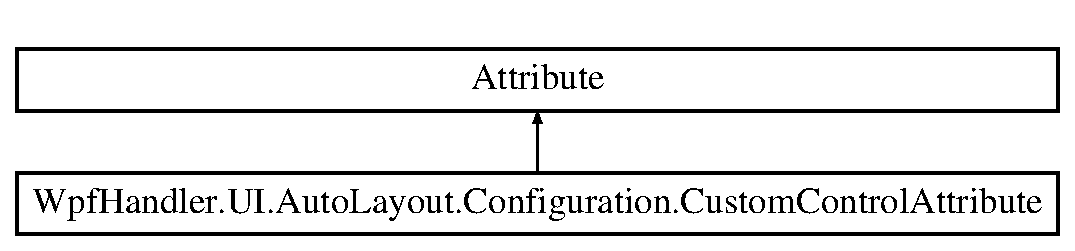
\includegraphics[height=2.000000cm]{d1/de8/class_wpf_handler_1_1_u_i_1_1_auto_layout_1_1_configuration_1_1_custom_control_attribute}
\end{center}
\end{figure}
\subsection*{Public Member Functions}
\begin{DoxyCompactItemize}
\item 
\mbox{\hyperlink{class_wpf_handler_1_1_u_i_1_1_auto_layout_1_1_configuration_1_1_custom_control_attribute_a7a46691a6fae1c36fb9812923e90cf8a}{Custom\+Control\+Attribute}} (Type control\+Type)
\begin{DoxyCompactList}\small\item\em Configurating attribute. \end{DoxyCompactList}\end{DoxyCompactItemize}
\subsection*{Properties}
\begin{DoxyCompactItemize}
\item 
Type \mbox{\hyperlink{class_wpf_handler_1_1_u_i_1_1_auto_layout_1_1_configuration_1_1_custom_control_attribute_a71f151123c78381231004ac155570be0}{Control\+Type}}\hspace{0.3cm}{\ttfamily  \mbox{[}get, set\mbox{]}}
\begin{DoxyCompactList}\small\item\em Control\textquotesingle{}s type that would be instiniated into G\+UI. \end{DoxyCompactList}\end{DoxyCompactItemize}
\subsection*{Private Attributes}
\begin{DoxyCompactItemize}
\item 
Type \mbox{\hyperlink{class_wpf_handler_1_1_u_i_1_1_auto_layout_1_1_configuration_1_1_custom_control_attribute_a3099e2b45323143744f788f5f9db22ab}{\+\_\+\+Control\+Type}}
\begin{DoxyCompactList}\small\item\em Buffer tht contains stored type. \end{DoxyCompactList}\end{DoxyCompactItemize}


\subsection{Detailed Description}
Overrides a default control for a field type for the parent member. 



\subsection{Constructor \& Destructor Documentation}
\mbox{\Hypertarget{class_wpf_handler_1_1_u_i_1_1_auto_layout_1_1_configuration_1_1_custom_control_attribute_a7a46691a6fae1c36fb9812923e90cf8a}\label{class_wpf_handler_1_1_u_i_1_1_auto_layout_1_1_configuration_1_1_custom_control_attribute_a7a46691a6fae1c36fb9812923e90cf8a}} 
\index{Wpf\+Handler\+::\+U\+I\+::\+Auto\+Layout\+::\+Configuration\+::\+Custom\+Control\+Attribute@{Wpf\+Handler\+::\+U\+I\+::\+Auto\+Layout\+::\+Configuration\+::\+Custom\+Control\+Attribute}!Custom\+Control\+Attribute@{Custom\+Control\+Attribute}}
\index{Custom\+Control\+Attribute@{Custom\+Control\+Attribute}!Wpf\+Handler\+::\+U\+I\+::\+Auto\+Layout\+::\+Configuration\+::\+Custom\+Control\+Attribute@{Wpf\+Handler\+::\+U\+I\+::\+Auto\+Layout\+::\+Configuration\+::\+Custom\+Control\+Attribute}}
\subsubsection{\texorpdfstring{Custom\+Control\+Attribute()}{CustomControlAttribute()}}
{\footnotesize\ttfamily Wpf\+Handler.\+U\+I.\+Auto\+Layout.\+Configuration.\+Custom\+Control\+Attribute.\+Custom\+Control\+Attribute (\begin{DoxyParamCaption}\item[{Type}]{control\+Type }\end{DoxyParamCaption})}



Configurating attribute. 


\begin{DoxyParams}{Parameters}
{\em control\+Type} & Type that would be instiniated during G\+UI spawn.\\
\hline
\end{DoxyParams}


\subsection{Member Data Documentation}
\mbox{\Hypertarget{class_wpf_handler_1_1_u_i_1_1_auto_layout_1_1_configuration_1_1_custom_control_attribute_a3099e2b45323143744f788f5f9db22ab}\label{class_wpf_handler_1_1_u_i_1_1_auto_layout_1_1_configuration_1_1_custom_control_attribute_a3099e2b45323143744f788f5f9db22ab}} 
\index{Wpf\+Handler\+::\+U\+I\+::\+Auto\+Layout\+::\+Configuration\+::\+Custom\+Control\+Attribute@{Wpf\+Handler\+::\+U\+I\+::\+Auto\+Layout\+::\+Configuration\+::\+Custom\+Control\+Attribute}!\+\_\+\+Control\+Type@{\+\_\+\+Control\+Type}}
\index{\+\_\+\+Control\+Type@{\+\_\+\+Control\+Type}!Wpf\+Handler\+::\+U\+I\+::\+Auto\+Layout\+::\+Configuration\+::\+Custom\+Control\+Attribute@{Wpf\+Handler\+::\+U\+I\+::\+Auto\+Layout\+::\+Configuration\+::\+Custom\+Control\+Attribute}}
\subsubsection{\texorpdfstring{\+\_\+\+Control\+Type}{\_ControlType}}
{\footnotesize\ttfamily Type Wpf\+Handler.\+U\+I.\+Auto\+Layout.\+Configuration.\+Custom\+Control\+Attribute.\+\_\+\+Control\+Type\hspace{0.3cm}{\ttfamily [private]}}



Buffer tht contains stored type. 



\subsection{Property Documentation}
\mbox{\Hypertarget{class_wpf_handler_1_1_u_i_1_1_auto_layout_1_1_configuration_1_1_custom_control_attribute_a71f151123c78381231004ac155570be0}\label{class_wpf_handler_1_1_u_i_1_1_auto_layout_1_1_configuration_1_1_custom_control_attribute_a71f151123c78381231004ac155570be0}} 
\index{Wpf\+Handler\+::\+U\+I\+::\+Auto\+Layout\+::\+Configuration\+::\+Custom\+Control\+Attribute@{Wpf\+Handler\+::\+U\+I\+::\+Auto\+Layout\+::\+Configuration\+::\+Custom\+Control\+Attribute}!Control\+Type@{Control\+Type}}
\index{Control\+Type@{Control\+Type}!Wpf\+Handler\+::\+U\+I\+::\+Auto\+Layout\+::\+Configuration\+::\+Custom\+Control\+Attribute@{Wpf\+Handler\+::\+U\+I\+::\+Auto\+Layout\+::\+Configuration\+::\+Custom\+Control\+Attribute}}
\subsubsection{\texorpdfstring{Control\+Type}{ControlType}}
{\footnotesize\ttfamily Type Wpf\+Handler.\+U\+I.\+Auto\+Layout.\+Configuration.\+Custom\+Control\+Attribute.\+Control\+Type\hspace{0.3cm}{\ttfamily [get]}, {\ttfamily [set]}}



Control\textquotesingle{}s type that would be instiniated into G\+UI. 



The documentation for this class was generated from the following file\+:\begin{DoxyCompactItemize}
\item 
D\+:/\+Work/\+Git\+Hub/wpf-\/handler/\+Wpf\+Handler/\+U\+I/\+Auto\+Layout/\+Configuration/Custom\+Control\+Attribute.\+cs\end{DoxyCompactItemize}

\hypertarget{class_wpf_handler_1_1_u_i_1_1_controls_1_1_logon_1_1_default_registration_panel_descriptor}{}\section{Wpf\+Handler.\+U\+I.\+Controls.\+Logon.\+Default\+Registration\+Panel\+Descriptor Class Reference}
\label{class_wpf_handler_1_1_u_i_1_1_controls_1_1_logon_1_1_default_registration_panel_descriptor}\index{Wpf\+Handler.\+U\+I.\+Controls.\+Logon.\+Default\+Registration\+Panel\+Descriptor@{Wpf\+Handler.\+U\+I.\+Controls.\+Logon.\+Default\+Registration\+Panel\+Descriptor}}


A desciptor used as default form for the refisration panel.  


Inheritance diagram for Wpf\+Handler.\+U\+I.\+Controls.\+Logon.\+Default\+Registration\+Panel\+Descriptor\+:\begin{figure}[H]
\begin{center}
\leavevmode
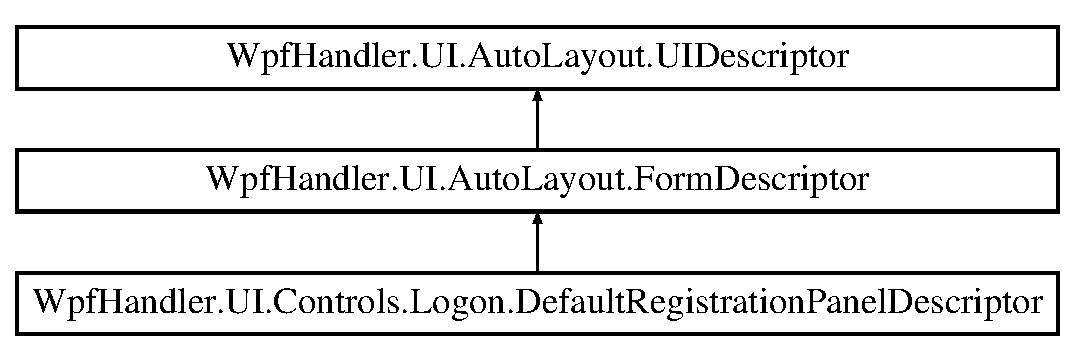
\includegraphics[height=3.000000cm]{d4/daf/class_wpf_handler_1_1_u_i_1_1_controls_1_1_logon_1_1_default_registration_panel_descriptor}
\end{center}
\end{figure}
\subsection*{Public Member Functions}
\begin{DoxyCompactItemize}
\item 
override \mbox{\hyperlink{struct_wpf_handler_1_1_u_i_1_1_auto_layout_1_1_form_descriptor_1_1_validation_report}{Validation\+Report}} \mbox{\hyperlink{class_wpf_handler_1_1_u_i_1_1_controls_1_1_logon_1_1_default_registration_panel_descriptor_abc8055d00358a941e9b507fed58ff662}{On\+Validation}} ()
\begin{DoxyCompactList}\small\item\em Handelr that will be called when a from should validate members data. \end{DoxyCompactList}\item 
override void \mbox{\hyperlink{class_wpf_handler_1_1_u_i_1_1_controls_1_1_logon_1_1_default_registration_panel_descriptor_aee1e6b6ba9214aac4a82b0213e4d3442}{On\+Confirm}} ()
\begin{DoxyCompactList}\small\item\em A handler that will called when the form will be confirmed. Handle the stored data. \end{DoxyCompactList}\item 
override void \mbox{\hyperlink{class_wpf_handler_1_1_u_i_1_1_controls_1_1_logon_1_1_default_registration_panel_descriptor_a9154a1e27afdf8d40da139042ee7e609}{On\+Cancel}} ()
\begin{DoxyCompactList}\small\item\em A handler that will called when the form will be canceled. Handle the stored data. \end{DoxyCompactList}\end{DoxyCompactItemize}
\subsection*{Properties}
\begin{DoxyCompactItemize}
\item 
string \mbox{\hyperlink{class_wpf_handler_1_1_u_i_1_1_controls_1_1_logon_1_1_default_registration_panel_descriptor_a4be5b2a0ce4dcbd9c596057b5bbeb8ce}{Login}}\hspace{0.3cm}{\ttfamily  \mbox{[}get, set\mbox{]}}
\begin{DoxyCompactList}\small\item\em A login for user profile. \end{DoxyCompactList}\item 
string \mbox{\hyperlink{class_wpf_handler_1_1_u_i_1_1_controls_1_1_logon_1_1_default_registration_panel_descriptor_ac525bd60f8febfaa251aeaebed55f515}{Password}}\hspace{0.3cm}{\ttfamily  \mbox{[}get, set\mbox{]}}
\begin{DoxyCompactList}\small\item\em A user\textquotesingle{}s password. \end{DoxyCompactList}\item 
string \mbox{\hyperlink{class_wpf_handler_1_1_u_i_1_1_controls_1_1_logon_1_1_default_registration_panel_descriptor_a6779df49ec2d45ee293929f3e7bafcf6}{Password\+Confirmation}}\hspace{0.3cm}{\ttfamily  \mbox{[}get, set\mbox{]}}
\begin{DoxyCompactList}\small\item\em An \mbox{\hyperlink{namespace_wpf_handler_1_1_u_i}{UI}} field that should contain the same password like in the \mbox{\hyperlink{class_wpf_handler_1_1_u_i_1_1_controls_1_1_logon_1_1_default_registration_panel_descriptor_ac525bd60f8febfaa251aeaebed55f515}{Password}} one. \end{DoxyCompactList}\item 
string \mbox{\hyperlink{class_wpf_handler_1_1_u_i_1_1_controls_1_1_logon_1_1_default_registration_panel_descriptor_a10f8af981d1154451adbc5896f53ffca}{First\+Name}}\hspace{0.3cm}{\ttfamily  \mbox{[}get, set\mbox{]}}
\begin{DoxyCompactList}\small\item\em A first name of an user. \end{DoxyCompactList}\item 
string \mbox{\hyperlink{class_wpf_handler_1_1_u_i_1_1_controls_1_1_logon_1_1_default_registration_panel_descriptor_a2a57913c309a9fb31fe5d4d9b0d6b7c6}{Middle\+Name}}\hspace{0.3cm}{\ttfamily  \mbox{[}get, set\mbox{]}}
\begin{DoxyCompactList}\small\item\em A middle name of an user. \end{DoxyCompactList}\item 
string \mbox{\hyperlink{class_wpf_handler_1_1_u_i_1_1_controls_1_1_logon_1_1_default_registration_panel_descriptor_a1cbf11f8c75a668f9a7398d3618857c9}{Last\+Name}}\hspace{0.3cm}{\ttfamily  \mbox{[}get, set\mbox{]}}
\begin{DoxyCompactList}\small\item\em A last and of an user. \end{DoxyCompactList}\item 
bool \mbox{\hyperlink{class_wpf_handler_1_1_u_i_1_1_controls_1_1_logon_1_1_default_registration_panel_descriptor_aecc64f8b53d3fb5e69d55d691a320a4b}{Is\+Passwords\+The\+Same}}\hspace{0.3cm}{\ttfamily  \mbox{[}get\mbox{]}}
\begin{DoxyCompactList}\small\item\em Check if passwords is the same and not null. \end{DoxyCompactList}\end{DoxyCompactItemize}
\subsection*{Additional Inherited Members}


\subsection{Detailed Description}
A desciptor used as default form for the refisration panel. 



\subsection{Member Function Documentation}
\mbox{\Hypertarget{class_wpf_handler_1_1_u_i_1_1_controls_1_1_logon_1_1_default_registration_panel_descriptor_a9154a1e27afdf8d40da139042ee7e609}\label{class_wpf_handler_1_1_u_i_1_1_controls_1_1_logon_1_1_default_registration_panel_descriptor_a9154a1e27afdf8d40da139042ee7e609}} 
\index{Wpf\+Handler\+::\+U\+I\+::\+Controls\+::\+Logon\+::\+Default\+Registration\+Panel\+Descriptor@{Wpf\+Handler\+::\+U\+I\+::\+Controls\+::\+Logon\+::\+Default\+Registration\+Panel\+Descriptor}!On\+Cancel@{On\+Cancel}}
\index{On\+Cancel@{On\+Cancel}!Wpf\+Handler\+::\+U\+I\+::\+Controls\+::\+Logon\+::\+Default\+Registration\+Panel\+Descriptor@{Wpf\+Handler\+::\+U\+I\+::\+Controls\+::\+Logon\+::\+Default\+Registration\+Panel\+Descriptor}}
\subsubsection{\texorpdfstring{On\+Cancel()}{OnCancel()}}
{\footnotesize\ttfamily override void Wpf\+Handler.\+U\+I.\+Controls.\+Logon.\+Default\+Registration\+Panel\+Descriptor.\+On\+Cancel (\begin{DoxyParamCaption}{ }\end{DoxyParamCaption})\hspace{0.3cm}{\ttfamily [virtual]}}



A handler that will called when the form will be canceled. Handle the stored data. 



Reimplemented from \mbox{\hyperlink{class_wpf_handler_1_1_u_i_1_1_auto_layout_1_1_form_descriptor_a4bbe131238be232c253ca4c65e8493f4}{Wpf\+Handler.\+U\+I.\+Auto\+Layout.\+Form\+Descriptor}}.

\mbox{\Hypertarget{class_wpf_handler_1_1_u_i_1_1_controls_1_1_logon_1_1_default_registration_panel_descriptor_aee1e6b6ba9214aac4a82b0213e4d3442}\label{class_wpf_handler_1_1_u_i_1_1_controls_1_1_logon_1_1_default_registration_panel_descriptor_aee1e6b6ba9214aac4a82b0213e4d3442}} 
\index{Wpf\+Handler\+::\+U\+I\+::\+Controls\+::\+Logon\+::\+Default\+Registration\+Panel\+Descriptor@{Wpf\+Handler\+::\+U\+I\+::\+Controls\+::\+Logon\+::\+Default\+Registration\+Panel\+Descriptor}!On\+Confirm@{On\+Confirm}}
\index{On\+Confirm@{On\+Confirm}!Wpf\+Handler\+::\+U\+I\+::\+Controls\+::\+Logon\+::\+Default\+Registration\+Panel\+Descriptor@{Wpf\+Handler\+::\+U\+I\+::\+Controls\+::\+Logon\+::\+Default\+Registration\+Panel\+Descriptor}}
\subsubsection{\texorpdfstring{On\+Confirm()}{OnConfirm()}}
{\footnotesize\ttfamily override void Wpf\+Handler.\+U\+I.\+Controls.\+Logon.\+Default\+Registration\+Panel\+Descriptor.\+On\+Confirm (\begin{DoxyParamCaption}{ }\end{DoxyParamCaption})\hspace{0.3cm}{\ttfamily [virtual]}}



A handler that will called when the form will be confirmed. Handle the stored data. 



Reimplemented from \mbox{\hyperlink{class_wpf_handler_1_1_u_i_1_1_auto_layout_1_1_form_descriptor_ae2d4791e3085dba435c09b6082bd8408}{Wpf\+Handler.\+U\+I.\+Auto\+Layout.\+Form\+Descriptor}}.

\mbox{\Hypertarget{class_wpf_handler_1_1_u_i_1_1_controls_1_1_logon_1_1_default_registration_panel_descriptor_abc8055d00358a941e9b507fed58ff662}\label{class_wpf_handler_1_1_u_i_1_1_controls_1_1_logon_1_1_default_registration_panel_descriptor_abc8055d00358a941e9b507fed58ff662}} 
\index{Wpf\+Handler\+::\+U\+I\+::\+Controls\+::\+Logon\+::\+Default\+Registration\+Panel\+Descriptor@{Wpf\+Handler\+::\+U\+I\+::\+Controls\+::\+Logon\+::\+Default\+Registration\+Panel\+Descriptor}!On\+Validation@{On\+Validation}}
\index{On\+Validation@{On\+Validation}!Wpf\+Handler\+::\+U\+I\+::\+Controls\+::\+Logon\+::\+Default\+Registration\+Panel\+Descriptor@{Wpf\+Handler\+::\+U\+I\+::\+Controls\+::\+Logon\+::\+Default\+Registration\+Panel\+Descriptor}}
\subsubsection{\texorpdfstring{On\+Validation()}{OnValidation()}}
{\footnotesize\ttfamily override \mbox{\hyperlink{struct_wpf_handler_1_1_u_i_1_1_auto_layout_1_1_form_descriptor_1_1_validation_report}{Validation\+Report}} Wpf\+Handler.\+U\+I.\+Controls.\+Logon.\+Default\+Registration\+Panel\+Descriptor.\+On\+Validation (\begin{DoxyParamCaption}{ }\end{DoxyParamCaption})\hspace{0.3cm}{\ttfamily [virtual]}}



Handelr that will be called when a from should validate members data. 

\begin{DoxyReturn}{Returns}
A validation report. 
\end{DoxyReturn}


Reimplemented from \mbox{\hyperlink{class_wpf_handler_1_1_u_i_1_1_auto_layout_1_1_form_descriptor_a63527cbe3f75e544b7f4ab417bfbb555}{Wpf\+Handler.\+U\+I.\+Auto\+Layout.\+Form\+Descriptor}}.



\subsection{Property Documentation}
\mbox{\Hypertarget{class_wpf_handler_1_1_u_i_1_1_controls_1_1_logon_1_1_default_registration_panel_descriptor_a10f8af981d1154451adbc5896f53ffca}\label{class_wpf_handler_1_1_u_i_1_1_controls_1_1_logon_1_1_default_registration_panel_descriptor_a10f8af981d1154451adbc5896f53ffca}} 
\index{Wpf\+Handler\+::\+U\+I\+::\+Controls\+::\+Logon\+::\+Default\+Registration\+Panel\+Descriptor@{Wpf\+Handler\+::\+U\+I\+::\+Controls\+::\+Logon\+::\+Default\+Registration\+Panel\+Descriptor}!First\+Name@{First\+Name}}
\index{First\+Name@{First\+Name}!Wpf\+Handler\+::\+U\+I\+::\+Controls\+::\+Logon\+::\+Default\+Registration\+Panel\+Descriptor@{Wpf\+Handler\+::\+U\+I\+::\+Controls\+::\+Logon\+::\+Default\+Registration\+Panel\+Descriptor}}
\subsubsection{\texorpdfstring{First\+Name}{FirstName}}
{\footnotesize\ttfamily string Wpf\+Handler.\+U\+I.\+Controls.\+Logon.\+Default\+Registration\+Panel\+Descriptor.\+First\+Name\hspace{0.3cm}{\ttfamily [get]}, {\ttfamily [set]}}



A first name of an user. 

\mbox{\Hypertarget{class_wpf_handler_1_1_u_i_1_1_controls_1_1_logon_1_1_default_registration_panel_descriptor_aecc64f8b53d3fb5e69d55d691a320a4b}\label{class_wpf_handler_1_1_u_i_1_1_controls_1_1_logon_1_1_default_registration_panel_descriptor_aecc64f8b53d3fb5e69d55d691a320a4b}} 
\index{Wpf\+Handler\+::\+U\+I\+::\+Controls\+::\+Logon\+::\+Default\+Registration\+Panel\+Descriptor@{Wpf\+Handler\+::\+U\+I\+::\+Controls\+::\+Logon\+::\+Default\+Registration\+Panel\+Descriptor}!Is\+Passwords\+The\+Same@{Is\+Passwords\+The\+Same}}
\index{Is\+Passwords\+The\+Same@{Is\+Passwords\+The\+Same}!Wpf\+Handler\+::\+U\+I\+::\+Controls\+::\+Logon\+::\+Default\+Registration\+Panel\+Descriptor@{Wpf\+Handler\+::\+U\+I\+::\+Controls\+::\+Logon\+::\+Default\+Registration\+Panel\+Descriptor}}
\subsubsection{\texorpdfstring{Is\+Passwords\+The\+Same}{IsPasswordsTheSame}}
{\footnotesize\ttfamily bool Wpf\+Handler.\+U\+I.\+Controls.\+Logon.\+Default\+Registration\+Panel\+Descriptor.\+Is\+Passwords\+The\+Same\hspace{0.3cm}{\ttfamily [get]}}



Check if passwords is the same and not null. 

\mbox{\Hypertarget{class_wpf_handler_1_1_u_i_1_1_controls_1_1_logon_1_1_default_registration_panel_descriptor_a1cbf11f8c75a668f9a7398d3618857c9}\label{class_wpf_handler_1_1_u_i_1_1_controls_1_1_logon_1_1_default_registration_panel_descriptor_a1cbf11f8c75a668f9a7398d3618857c9}} 
\index{Wpf\+Handler\+::\+U\+I\+::\+Controls\+::\+Logon\+::\+Default\+Registration\+Panel\+Descriptor@{Wpf\+Handler\+::\+U\+I\+::\+Controls\+::\+Logon\+::\+Default\+Registration\+Panel\+Descriptor}!Last\+Name@{Last\+Name}}
\index{Last\+Name@{Last\+Name}!Wpf\+Handler\+::\+U\+I\+::\+Controls\+::\+Logon\+::\+Default\+Registration\+Panel\+Descriptor@{Wpf\+Handler\+::\+U\+I\+::\+Controls\+::\+Logon\+::\+Default\+Registration\+Panel\+Descriptor}}
\subsubsection{\texorpdfstring{Last\+Name}{LastName}}
{\footnotesize\ttfamily string Wpf\+Handler.\+U\+I.\+Controls.\+Logon.\+Default\+Registration\+Panel\+Descriptor.\+Last\+Name\hspace{0.3cm}{\ttfamily [get]}, {\ttfamily [set]}}



A last and of an user. 

\mbox{\Hypertarget{class_wpf_handler_1_1_u_i_1_1_controls_1_1_logon_1_1_default_registration_panel_descriptor_a4be5b2a0ce4dcbd9c596057b5bbeb8ce}\label{class_wpf_handler_1_1_u_i_1_1_controls_1_1_logon_1_1_default_registration_panel_descriptor_a4be5b2a0ce4dcbd9c596057b5bbeb8ce}} 
\index{Wpf\+Handler\+::\+U\+I\+::\+Controls\+::\+Logon\+::\+Default\+Registration\+Panel\+Descriptor@{Wpf\+Handler\+::\+U\+I\+::\+Controls\+::\+Logon\+::\+Default\+Registration\+Panel\+Descriptor}!Login@{Login}}
\index{Login@{Login}!Wpf\+Handler\+::\+U\+I\+::\+Controls\+::\+Logon\+::\+Default\+Registration\+Panel\+Descriptor@{Wpf\+Handler\+::\+U\+I\+::\+Controls\+::\+Logon\+::\+Default\+Registration\+Panel\+Descriptor}}
\subsubsection{\texorpdfstring{Login}{Login}}
{\footnotesize\ttfamily string Wpf\+Handler.\+U\+I.\+Controls.\+Logon.\+Default\+Registration\+Panel\+Descriptor.\+Login\hspace{0.3cm}{\ttfamily [get]}, {\ttfamily [set]}}



A login for user profile. 

\mbox{\Hypertarget{class_wpf_handler_1_1_u_i_1_1_controls_1_1_logon_1_1_default_registration_panel_descriptor_a2a57913c309a9fb31fe5d4d9b0d6b7c6}\label{class_wpf_handler_1_1_u_i_1_1_controls_1_1_logon_1_1_default_registration_panel_descriptor_a2a57913c309a9fb31fe5d4d9b0d6b7c6}} 
\index{Wpf\+Handler\+::\+U\+I\+::\+Controls\+::\+Logon\+::\+Default\+Registration\+Panel\+Descriptor@{Wpf\+Handler\+::\+U\+I\+::\+Controls\+::\+Logon\+::\+Default\+Registration\+Panel\+Descriptor}!Middle\+Name@{Middle\+Name}}
\index{Middle\+Name@{Middle\+Name}!Wpf\+Handler\+::\+U\+I\+::\+Controls\+::\+Logon\+::\+Default\+Registration\+Panel\+Descriptor@{Wpf\+Handler\+::\+U\+I\+::\+Controls\+::\+Logon\+::\+Default\+Registration\+Panel\+Descriptor}}
\subsubsection{\texorpdfstring{Middle\+Name}{MiddleName}}
{\footnotesize\ttfamily string Wpf\+Handler.\+U\+I.\+Controls.\+Logon.\+Default\+Registration\+Panel\+Descriptor.\+Middle\+Name\hspace{0.3cm}{\ttfamily [get]}, {\ttfamily [set]}}



A middle name of an user. 

\mbox{\Hypertarget{class_wpf_handler_1_1_u_i_1_1_controls_1_1_logon_1_1_default_registration_panel_descriptor_ac525bd60f8febfaa251aeaebed55f515}\label{class_wpf_handler_1_1_u_i_1_1_controls_1_1_logon_1_1_default_registration_panel_descriptor_ac525bd60f8febfaa251aeaebed55f515}} 
\index{Wpf\+Handler\+::\+U\+I\+::\+Controls\+::\+Logon\+::\+Default\+Registration\+Panel\+Descriptor@{Wpf\+Handler\+::\+U\+I\+::\+Controls\+::\+Logon\+::\+Default\+Registration\+Panel\+Descriptor}!Password@{Password}}
\index{Password@{Password}!Wpf\+Handler\+::\+U\+I\+::\+Controls\+::\+Logon\+::\+Default\+Registration\+Panel\+Descriptor@{Wpf\+Handler\+::\+U\+I\+::\+Controls\+::\+Logon\+::\+Default\+Registration\+Panel\+Descriptor}}
\subsubsection{\texorpdfstring{Password}{Password}}
{\footnotesize\ttfamily string Wpf\+Handler.\+U\+I.\+Controls.\+Logon.\+Default\+Registration\+Panel\+Descriptor.\+Password\hspace{0.3cm}{\ttfamily [get]}, {\ttfamily [set]}}



A user\textquotesingle{}s password. 

\mbox{\Hypertarget{class_wpf_handler_1_1_u_i_1_1_controls_1_1_logon_1_1_default_registration_panel_descriptor_a6779df49ec2d45ee293929f3e7bafcf6}\label{class_wpf_handler_1_1_u_i_1_1_controls_1_1_logon_1_1_default_registration_panel_descriptor_a6779df49ec2d45ee293929f3e7bafcf6}} 
\index{Wpf\+Handler\+::\+U\+I\+::\+Controls\+::\+Logon\+::\+Default\+Registration\+Panel\+Descriptor@{Wpf\+Handler\+::\+U\+I\+::\+Controls\+::\+Logon\+::\+Default\+Registration\+Panel\+Descriptor}!Password\+Confirmation@{Password\+Confirmation}}
\index{Password\+Confirmation@{Password\+Confirmation}!Wpf\+Handler\+::\+U\+I\+::\+Controls\+::\+Logon\+::\+Default\+Registration\+Panel\+Descriptor@{Wpf\+Handler\+::\+U\+I\+::\+Controls\+::\+Logon\+::\+Default\+Registration\+Panel\+Descriptor}}
\subsubsection{\texorpdfstring{Password\+Confirmation}{PasswordConfirmation}}
{\footnotesize\ttfamily string Wpf\+Handler.\+U\+I.\+Controls.\+Logon.\+Default\+Registration\+Panel\+Descriptor.\+Password\+Confirmation\hspace{0.3cm}{\ttfamily [get]}, {\ttfamily [set]}}



An \mbox{\hyperlink{namespace_wpf_handler_1_1_u_i}{UI}} field that should contain the same password like in the \mbox{\hyperlink{class_wpf_handler_1_1_u_i_1_1_controls_1_1_logon_1_1_default_registration_panel_descriptor_ac525bd60f8febfaa251aeaebed55f515}{Password}} one. 



The documentation for this class was generated from the following file\+:\begin{DoxyCompactItemize}
\item 
D\+:/\+Work/\+Git\+Hub/wpf-\/handler/\+Wpf\+Handler/\+U\+I/\+Controls/\+Logon/Default\+Registration\+Panel\+Descriptor.\+cs\end{DoxyCompactItemize}

\hypertarget{class_wpf_handler_1_1_dictionaries_1_1_domain_container}{}\section{Wpf\+Handler.\+Dictionaries.\+Domain\+Container Class Reference}
\label{class_wpf_handler_1_1_dictionaries_1_1_domain_container}\index{Wpf\+Handler.\+Dictionaries.\+Domain\+Container@{Wpf\+Handler.\+Dictionaries.\+Domain\+Container}}


Class that provide information about dictionary domain.  


\subsection*{Public Attributes}
\begin{DoxyCompactItemize}
\item 
string \mbox{\hyperlink{class_wpf_handler_1_1_dictionaries_1_1_domain_container_ac87b2b5f12c34ef7c585f789a48667eb}{key}}
\begin{DoxyCompactList}\small\item\em Key code of this dictionary. \end{DoxyCompactList}\item 
string \mbox{\hyperlink{class_wpf_handler_1_1_dictionaries_1_1_domain_container_a364742e0754175046839e274bd1f1a1d}{plugin\+Domain}}
\begin{DoxyCompactList}\small\item\em Full domain of plugin. \end{DoxyCompactList}\item 
string \mbox{\hyperlink{class_wpf_handler_1_1_dictionaries_1_1_domain_container_a4b434bec866ecf4747ae30248fcbf760}{path}}
\begin{DoxyCompactList}\small\item\em Path to dictionary xaml. \end{DoxyCompactList}\end{DoxyCompactItemize}


\subsection{Detailed Description}
Class that provide information about dictionary domain. 



\subsection{Member Data Documentation}
\mbox{\Hypertarget{class_wpf_handler_1_1_dictionaries_1_1_domain_container_ac87b2b5f12c34ef7c585f789a48667eb}\label{class_wpf_handler_1_1_dictionaries_1_1_domain_container_ac87b2b5f12c34ef7c585f789a48667eb}} 
\index{Wpf\+Handler\+::\+Dictionaries\+::\+Domain\+Container@{Wpf\+Handler\+::\+Dictionaries\+::\+Domain\+Container}!key@{key}}
\index{key@{key}!Wpf\+Handler\+::\+Dictionaries\+::\+Domain\+Container@{Wpf\+Handler\+::\+Dictionaries\+::\+Domain\+Container}}
\subsubsection{\texorpdfstring{key}{key}}
{\footnotesize\ttfamily string Wpf\+Handler.\+Dictionaries.\+Domain\+Container.\+key}



Key code of this dictionary. 

\mbox{\Hypertarget{class_wpf_handler_1_1_dictionaries_1_1_domain_container_a4b434bec866ecf4747ae30248fcbf760}\label{class_wpf_handler_1_1_dictionaries_1_1_domain_container_a4b434bec866ecf4747ae30248fcbf760}} 
\index{Wpf\+Handler\+::\+Dictionaries\+::\+Domain\+Container@{Wpf\+Handler\+::\+Dictionaries\+::\+Domain\+Container}!path@{path}}
\index{path@{path}!Wpf\+Handler\+::\+Dictionaries\+::\+Domain\+Container@{Wpf\+Handler\+::\+Dictionaries\+::\+Domain\+Container}}
\subsubsection{\texorpdfstring{path}{path}}
{\footnotesize\ttfamily string Wpf\+Handler.\+Dictionaries.\+Domain\+Container.\+path}



Path to dictionary xaml. 

\mbox{\Hypertarget{class_wpf_handler_1_1_dictionaries_1_1_domain_container_a364742e0754175046839e274bd1f1a1d}\label{class_wpf_handler_1_1_dictionaries_1_1_domain_container_a364742e0754175046839e274bd1f1a1d}} 
\index{Wpf\+Handler\+::\+Dictionaries\+::\+Domain\+Container@{Wpf\+Handler\+::\+Dictionaries\+::\+Domain\+Container}!plugin\+Domain@{plugin\+Domain}}
\index{plugin\+Domain@{plugin\+Domain}!Wpf\+Handler\+::\+Dictionaries\+::\+Domain\+Container@{Wpf\+Handler\+::\+Dictionaries\+::\+Domain\+Container}}
\subsubsection{\texorpdfstring{plugin\+Domain}{pluginDomain}}
{\footnotesize\ttfamily string Wpf\+Handler.\+Dictionaries.\+Domain\+Container.\+plugin\+Domain}



Full domain of plugin. 



The documentation for this class was generated from the following file\+:\begin{DoxyCompactItemize}
\item 
D\+:/\+Work/\+Git\+Hub/wpf-\/handler/\+Wpf\+Handler/\+Dictionaries/Domain\+Container.\+cs\end{DoxyCompactItemize}

\hypertarget{class_wpf_handler_1_1_u_i_1_1_auto_layout_1_1_configuration_1_1_end_group_attribute}{}\section{Wpf\+Handler.\+U\+I.\+Auto\+Layout.\+Configuration.\+End\+Group\+Attribute Class Reference}
\label{class_wpf_handler_1_1_u_i_1_1_auto_layout_1_1_configuration_1_1_end_group_attribute}\index{Wpf\+Handler.\+U\+I.\+Auto\+Layout.\+Configuration.\+End\+Group\+Attribute@{Wpf\+Handler.\+U\+I.\+Auto\+Layout.\+Configuration.\+End\+Group\+Attribute}}


Close a last started layout group.  


Inheritance diagram for Wpf\+Handler.\+U\+I.\+Auto\+Layout.\+Configuration.\+End\+Group\+Attribute\+:\begin{figure}[H]
\begin{center}
\leavevmode
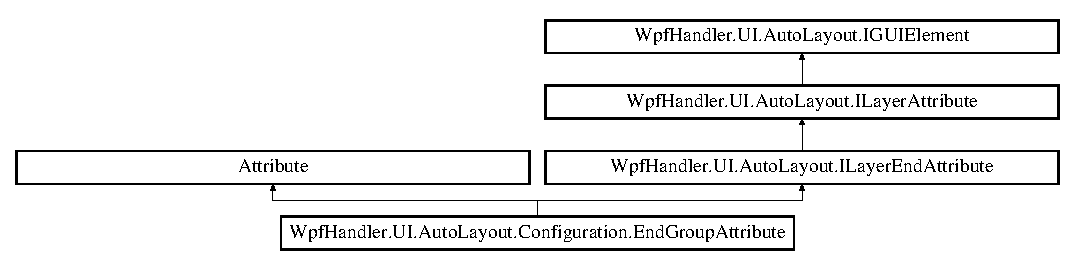
\includegraphics[height=3.128492cm]{db/de0/class_wpf_handler_1_1_u_i_1_1_auto_layout_1_1_configuration_1_1_end_group_attribute}
\end{center}
\end{figure}
\subsection*{Public Member Functions}
\begin{DoxyCompactItemize}
\item 
void \mbox{\hyperlink{class_wpf_handler_1_1_u_i_1_1_auto_layout_1_1_configuration_1_1_end_group_attribute_acaed685d0daf2b14d8f232389d56c478}{On\+Layout}} (ref \mbox{\hyperlink{class_wpf_handler_1_1_u_i_1_1_auto_layout_1_1_layout_layer}{Layout\+Layer}} layer, params object\mbox{[}$\,$\mbox{]} args)
\begin{DoxyCompactList}\small\item\em Trying to go to the upper \mbox{\hyperlink{namespace_wpf_handler_1_1_u_i}{UI}}\textquotesingle{}s layer. \end{DoxyCompactList}\end{DoxyCompactItemize}
\subsection*{Properties}
\begin{DoxyCompactItemize}
\item 
\mbox{\hyperlink{class_wpf_handler_1_1_u_i_1_1_auto_layout_1_1_layout_layer}{Layout\+Layer}} \mbox{\hyperlink{class_wpf_handler_1_1_u_i_1_1_auto_layout_1_1_configuration_1_1_end_group_attribute_aa49aeed9019ee998b6b85920251ce7c2}{Layer}}\hspace{0.3cm}{\ttfamily  \mbox{[}get\mbox{]}}
\begin{DoxyCompactList}\small\item\em Reference to the layer that had been got by handler doring Go\+Upper operation. \end{DoxyCompactList}\end{DoxyCompactItemize}
\subsection*{Private Attributes}
\begin{DoxyCompactItemize}
\item 
\mbox{\hyperlink{class_wpf_handler_1_1_u_i_1_1_auto_layout_1_1_layout_layer}{Layout\+Layer}} \mbox{\hyperlink{class_wpf_handler_1_1_u_i_1_1_auto_layout_1_1_configuration_1_1_end_group_attribute_a8f6eb211c88e7d5ade018a8f79d34a17}{\+\_\+\+Layer}}
\begin{DoxyCompactList}\small\item\em Bufer that contains operated layer. \end{DoxyCompactList}\end{DoxyCompactItemize}


\subsection{Detailed Description}
Close a last started layout group. 



\subsection{Member Function Documentation}
\mbox{\Hypertarget{class_wpf_handler_1_1_u_i_1_1_auto_layout_1_1_configuration_1_1_end_group_attribute_acaed685d0daf2b14d8f232389d56c478}\label{class_wpf_handler_1_1_u_i_1_1_auto_layout_1_1_configuration_1_1_end_group_attribute_acaed685d0daf2b14d8f232389d56c478}} 
\index{Wpf\+Handler\+::\+U\+I\+::\+Auto\+Layout\+::\+Configuration\+::\+End\+Group\+Attribute@{Wpf\+Handler\+::\+U\+I\+::\+Auto\+Layout\+::\+Configuration\+::\+End\+Group\+Attribute}!On\+Layout@{On\+Layout}}
\index{On\+Layout@{On\+Layout}!Wpf\+Handler\+::\+U\+I\+::\+Auto\+Layout\+::\+Configuration\+::\+End\+Group\+Attribute@{Wpf\+Handler\+::\+U\+I\+::\+Auto\+Layout\+::\+Configuration\+::\+End\+Group\+Attribute}}
\subsubsection{\texorpdfstring{On\+Layout()}{OnLayout()}}
{\footnotesize\ttfamily void Wpf\+Handler.\+U\+I.\+Auto\+Layout.\+Configuration.\+End\+Group\+Attribute.\+On\+Layout (\begin{DoxyParamCaption}\item[{ref \mbox{\hyperlink{class_wpf_handler_1_1_u_i_1_1_auto_layout_1_1_layout_layer}{Layout\+Layer}}}]{layer,  }\item[{params object \mbox{[}$\,$\mbox{]}}]{args }\end{DoxyParamCaption})}



Trying to go to the upper \mbox{\hyperlink{namespace_wpf_handler_1_1_u_i}{UI}}\textquotesingle{}s layer. 


\begin{DoxyParams}{Parameters}
{\em layer} & Current layer. Reference will be changed on relevant one.\\
\hline
{\em args} & Not using in that element.\\
\hline
\end{DoxyParams}


Implements \mbox{\hyperlink{interface_wpf_handler_1_1_u_i_1_1_auto_layout_1_1_i_g_u_i_element_a0ff16956f8e8187d51e1b36b6b9f894e}{Wpf\+Handler.\+U\+I.\+Auto\+Layout.\+I\+G\+U\+I\+Element}}.



\subsection{Member Data Documentation}
\mbox{\Hypertarget{class_wpf_handler_1_1_u_i_1_1_auto_layout_1_1_configuration_1_1_end_group_attribute_a8f6eb211c88e7d5ade018a8f79d34a17}\label{class_wpf_handler_1_1_u_i_1_1_auto_layout_1_1_configuration_1_1_end_group_attribute_a8f6eb211c88e7d5ade018a8f79d34a17}} 
\index{Wpf\+Handler\+::\+U\+I\+::\+Auto\+Layout\+::\+Configuration\+::\+End\+Group\+Attribute@{Wpf\+Handler\+::\+U\+I\+::\+Auto\+Layout\+::\+Configuration\+::\+End\+Group\+Attribute}!\+\_\+\+Layer@{\+\_\+\+Layer}}
\index{\+\_\+\+Layer@{\+\_\+\+Layer}!Wpf\+Handler\+::\+U\+I\+::\+Auto\+Layout\+::\+Configuration\+::\+End\+Group\+Attribute@{Wpf\+Handler\+::\+U\+I\+::\+Auto\+Layout\+::\+Configuration\+::\+End\+Group\+Attribute}}
\subsubsection{\texorpdfstring{\+\_\+\+Layer}{\_Layer}}
{\footnotesize\ttfamily \mbox{\hyperlink{class_wpf_handler_1_1_u_i_1_1_auto_layout_1_1_layout_layer}{Layout\+Layer}} Wpf\+Handler.\+U\+I.\+Auto\+Layout.\+Configuration.\+End\+Group\+Attribute.\+\_\+\+Layer\hspace{0.3cm}{\ttfamily [private]}}



Bufer that contains operated layer. 



\subsection{Property Documentation}
\mbox{\Hypertarget{class_wpf_handler_1_1_u_i_1_1_auto_layout_1_1_configuration_1_1_end_group_attribute_aa49aeed9019ee998b6b85920251ce7c2}\label{class_wpf_handler_1_1_u_i_1_1_auto_layout_1_1_configuration_1_1_end_group_attribute_aa49aeed9019ee998b6b85920251ce7c2}} 
\index{Wpf\+Handler\+::\+U\+I\+::\+Auto\+Layout\+::\+Configuration\+::\+End\+Group\+Attribute@{Wpf\+Handler\+::\+U\+I\+::\+Auto\+Layout\+::\+Configuration\+::\+End\+Group\+Attribute}!Layer@{Layer}}
\index{Layer@{Layer}!Wpf\+Handler\+::\+U\+I\+::\+Auto\+Layout\+::\+Configuration\+::\+End\+Group\+Attribute@{Wpf\+Handler\+::\+U\+I\+::\+Auto\+Layout\+::\+Configuration\+::\+End\+Group\+Attribute}}
\subsubsection{\texorpdfstring{Layer}{Layer}}
{\footnotesize\ttfamily \mbox{\hyperlink{class_wpf_handler_1_1_u_i_1_1_auto_layout_1_1_layout_layer}{Layout\+Layer}} Wpf\+Handler.\+U\+I.\+Auto\+Layout.\+Configuration.\+End\+Group\+Attribute.\+Layer\hspace{0.3cm}{\ttfamily [get]}}



Reference to the layer that had been got by handler doring Go\+Upper operation. 



The documentation for this class was generated from the following file\+:\begin{DoxyCompactItemize}
\item 
D\+:/\+Work/\+Git\+Hub/wpf-\/handler/\+Wpf\+Handler/\+U\+I/\+Auto\+Layout/\+Configuration/End\+Group\+Attribute.\+cs\end{DoxyCompactItemize}

\hypertarget{class_wpf_handler_1_1_u_i_1_1_auto_layout_1_1_markups_1_1_enums_compatible_attribute}{}\section{Wpf\+Handler.\+U\+I.\+Auto\+Layout.\+Markups.\+Enums\+Compatible\+Attribute Class Reference}
\label{class_wpf_handler_1_1_u_i_1_1_auto_layout_1_1_markups_1_1_enums_compatible_attribute}\index{Wpf\+Handler.\+U\+I.\+Auto\+Layout.\+Markups.\+Enums\+Compatible\+Attribute@{Wpf\+Handler.\+U\+I.\+Auto\+Layout.\+Markups.\+Enums\+Compatible\+Attribute}}


Marks a G\+UI element as compatible with enum source fields.  


Inheritance diagram for Wpf\+Handler.\+U\+I.\+Auto\+Layout.\+Markups.\+Enums\+Compatible\+Attribute\+:\begin{figure}[H]
\begin{center}
\leavevmode
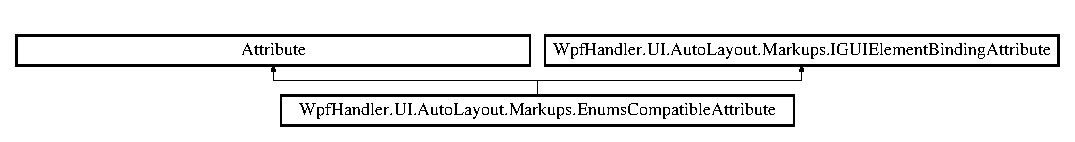
\includegraphics[height=1.462141cm]{d0/de7/class_wpf_handler_1_1_u_i_1_1_auto_layout_1_1_markups_1_1_enums_compatible_attribute}
\end{center}
\end{figure}


\subsection{Detailed Description}
Marks a G\+UI element as compatible with enum source fields. 



The documentation for this class was generated from the following file\+:\begin{DoxyCompactItemize}
\item 
D\+:/\+Work/\+Git\+Hub/wpf-\/handler/\+Wpf\+Handler/\+U\+I/\+Auto\+Layout/\+Markups/Enums\+Compatible\+Attribute.\+cs\end{DoxyCompactItemize}

\hypertarget{class_wpf_handler_1_1_u_i_1_1_animations_1_1_grid_length_animation_1_1_expander_double_animation}{}\section{Wpf\+Handler.\+U\+I.\+Animations.\+Grid\+Length\+Animation.\+Expander\+Double\+Animation Class Reference}
\label{class_wpf_handler_1_1_u_i_1_1_animations_1_1_grid_length_animation_1_1_expander_double_animation}\index{Wpf\+Handler.\+U\+I.\+Animations.\+Grid\+Length\+Animation.\+Expander\+Double\+Animation@{Wpf\+Handler.\+U\+I.\+Animations.\+Grid\+Length\+Animation.\+Expander\+Double\+Animation}}


Animates a double value  


Inheritance diagram for Wpf\+Handler.\+U\+I.\+Animations.\+Grid\+Length\+Animation.\+Expander\+Double\+Animation\+:\begin{figure}[H]
\begin{center}
\leavevmode
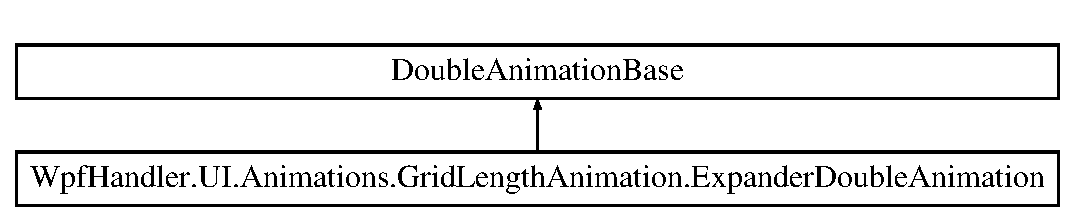
\includegraphics[height=2.000000cm]{d8/d40/class_wpf_handler_1_1_u_i_1_1_animations_1_1_grid_length_animation_1_1_expander_double_animation}
\end{center}
\end{figure}
\subsection*{Static Public Attributes}
\begin{DoxyCompactItemize}
\item 
static readonly Dependency\+Property \mbox{\hyperlink{class_wpf_handler_1_1_u_i_1_1_animations_1_1_grid_length_animation_1_1_expander_double_animation_a07d113740c7fc7eb161b5a0e38148462}{From\+Property}}
\begin{DoxyCompactList}\small\item\em Dependency property for the From property \end{DoxyCompactList}\item 
static readonly Dependency\+Property \mbox{\hyperlink{class_wpf_handler_1_1_u_i_1_1_animations_1_1_grid_length_animation_1_1_expander_double_animation_ae633ca54f3b0259e8a469f95a3a2f14b}{To\+Property}}
\begin{DoxyCompactList}\small\item\em Dependency property for the To property \end{DoxyCompactList}\item 
static readonly Dependency\+Property \mbox{\hyperlink{class_wpf_handler_1_1_u_i_1_1_animations_1_1_grid_length_animation_1_1_expander_double_animation_a31911e20e670e43ed1fc9b112f28ef68}{Reverse\+Value\+Property}}
\begin{DoxyCompactList}\small\item\em Sets the reverse value for the second animation \end{DoxyCompactList}\end{DoxyCompactItemize}
\subsection*{Protected Member Functions}
\begin{DoxyCompactItemize}
\item 
override Freezable \mbox{\hyperlink{class_wpf_handler_1_1_u_i_1_1_animations_1_1_grid_length_animation_1_1_expander_double_animation_a5645ce2b57d614b780066d0488b6dbd2}{Create\+Instance\+Core}} ()
\begin{DoxyCompactList}\small\item\em Creates an instance of the animation \end{DoxyCompactList}\item 
override double \mbox{\hyperlink{class_wpf_handler_1_1_u_i_1_1_animations_1_1_grid_length_animation_1_1_expander_double_animation_a49199d29a79cc39beb113376997e5973}{Get\+Current\+Value\+Core}} (double default\+Origin\+Value, double default\+Destination\+Value, Animation\+Clock animation\+Clock)
\begin{DoxyCompactList}\small\item\em Animates the double value \end{DoxyCompactList}\end{DoxyCompactItemize}
\subsection*{Properties}
\begin{DoxyCompactItemize}
\item 
double \mbox{\hyperlink{class_wpf_handler_1_1_u_i_1_1_animations_1_1_grid_length_animation_1_1_expander_double_animation_a2273bd2ccab6914f1b20bacf5c213ec7}{From}}\hspace{0.3cm}{\ttfamily  \mbox{[}get, set\mbox{]}}
\begin{DoxyCompactList}\small\item\em C\+LR Wrapper for the From depenendency property \end{DoxyCompactList}\item 
double \mbox{\hyperlink{class_wpf_handler_1_1_u_i_1_1_animations_1_1_grid_length_animation_1_1_expander_double_animation_aecdf2e18236eeb5bafc523b556c80641}{To}}\hspace{0.3cm}{\ttfamily  \mbox{[}get, set\mbox{]}}
\begin{DoxyCompactList}\small\item\em C\+LR Wrapper for the To property \end{DoxyCompactList}\item 
double \mbox{\hyperlink{class_wpf_handler_1_1_u_i_1_1_animations_1_1_grid_length_animation_1_1_expander_double_animation_afe3c498fad9f7f6be927b5d1d1f7514b}{Reverse\+Value}}\hspace{0.3cm}{\ttfamily  \mbox{[}get, set\mbox{]}}
\begin{DoxyCompactList}\small\item\em Sets the reverse value for the second animation \end{DoxyCompactList}\end{DoxyCompactItemize}


\subsection{Detailed Description}
Animates a double value 



\subsection{Member Function Documentation}
\mbox{\Hypertarget{class_wpf_handler_1_1_u_i_1_1_animations_1_1_grid_length_animation_1_1_expander_double_animation_a5645ce2b57d614b780066d0488b6dbd2}\label{class_wpf_handler_1_1_u_i_1_1_animations_1_1_grid_length_animation_1_1_expander_double_animation_a5645ce2b57d614b780066d0488b6dbd2}} 
\index{Wpf\+Handler\+::\+U\+I\+::\+Animations\+::\+Grid\+Length\+Animation\+::\+Expander\+Double\+Animation@{Wpf\+Handler\+::\+U\+I\+::\+Animations\+::\+Grid\+Length\+Animation\+::\+Expander\+Double\+Animation}!Create\+Instance\+Core@{Create\+Instance\+Core}}
\index{Create\+Instance\+Core@{Create\+Instance\+Core}!Wpf\+Handler\+::\+U\+I\+::\+Animations\+::\+Grid\+Length\+Animation\+::\+Expander\+Double\+Animation@{Wpf\+Handler\+::\+U\+I\+::\+Animations\+::\+Grid\+Length\+Animation\+::\+Expander\+Double\+Animation}}
\subsubsection{\texorpdfstring{Create\+Instance\+Core()}{CreateInstanceCore()}}
{\footnotesize\ttfamily override Freezable Wpf\+Handler.\+U\+I.\+Animations.\+Grid\+Length\+Animation.\+Expander\+Double\+Animation.\+Create\+Instance\+Core (\begin{DoxyParamCaption}{ }\end{DoxyParamCaption})\hspace{0.3cm}{\ttfamily [protected]}}



Creates an instance of the animation 

\begin{DoxyReturn}{Returns}

\end{DoxyReturn}
\mbox{\Hypertarget{class_wpf_handler_1_1_u_i_1_1_animations_1_1_grid_length_animation_1_1_expander_double_animation_a49199d29a79cc39beb113376997e5973}\label{class_wpf_handler_1_1_u_i_1_1_animations_1_1_grid_length_animation_1_1_expander_double_animation_a49199d29a79cc39beb113376997e5973}} 
\index{Wpf\+Handler\+::\+U\+I\+::\+Animations\+::\+Grid\+Length\+Animation\+::\+Expander\+Double\+Animation@{Wpf\+Handler\+::\+U\+I\+::\+Animations\+::\+Grid\+Length\+Animation\+::\+Expander\+Double\+Animation}!Get\+Current\+Value\+Core@{Get\+Current\+Value\+Core}}
\index{Get\+Current\+Value\+Core@{Get\+Current\+Value\+Core}!Wpf\+Handler\+::\+U\+I\+::\+Animations\+::\+Grid\+Length\+Animation\+::\+Expander\+Double\+Animation@{Wpf\+Handler\+::\+U\+I\+::\+Animations\+::\+Grid\+Length\+Animation\+::\+Expander\+Double\+Animation}}
\subsubsection{\texorpdfstring{Get\+Current\+Value\+Core()}{GetCurrentValueCore()}}
{\footnotesize\ttfamily override double Wpf\+Handler.\+U\+I.\+Animations.\+Grid\+Length\+Animation.\+Expander\+Double\+Animation.\+Get\+Current\+Value\+Core (\begin{DoxyParamCaption}\item[{double}]{default\+Origin\+Value,  }\item[{double}]{default\+Destination\+Value,  }\item[{Animation\+Clock}]{animation\+Clock }\end{DoxyParamCaption})\hspace{0.3cm}{\ttfamily [protected]}}



Animates the double value 


\begin{DoxyParams}{Parameters}
{\em default\+Origin\+Value} & The original value to animate\\
\hline
{\em default\+Destination\+Value} & The final value\\
\hline
{\em animation\+Clock} & The animation clock (timer)\\
\hline
\end{DoxyParams}
\begin{DoxyReturn}{Returns}
Returns the new double to set
\end{DoxyReturn}


\subsection{Member Data Documentation}
\mbox{\Hypertarget{class_wpf_handler_1_1_u_i_1_1_animations_1_1_grid_length_animation_1_1_expander_double_animation_a07d113740c7fc7eb161b5a0e38148462}\label{class_wpf_handler_1_1_u_i_1_1_animations_1_1_grid_length_animation_1_1_expander_double_animation_a07d113740c7fc7eb161b5a0e38148462}} 
\index{Wpf\+Handler\+::\+U\+I\+::\+Animations\+::\+Grid\+Length\+Animation\+::\+Expander\+Double\+Animation@{Wpf\+Handler\+::\+U\+I\+::\+Animations\+::\+Grid\+Length\+Animation\+::\+Expander\+Double\+Animation}!From\+Property@{From\+Property}}
\index{From\+Property@{From\+Property}!Wpf\+Handler\+::\+U\+I\+::\+Animations\+::\+Grid\+Length\+Animation\+::\+Expander\+Double\+Animation@{Wpf\+Handler\+::\+U\+I\+::\+Animations\+::\+Grid\+Length\+Animation\+::\+Expander\+Double\+Animation}}
\subsubsection{\texorpdfstring{From\+Property}{FromProperty}}
{\footnotesize\ttfamily readonly Dependency\+Property Wpf\+Handler.\+U\+I.\+Animations.\+Grid\+Length\+Animation.\+Expander\+Double\+Animation.\+From\+Property\hspace{0.3cm}{\ttfamily [static]}}

{\bfseries Initial value\+:}
\begin{DoxyCode}
= DependencyProperty.Register(\textcolor{stringliteral}{"From"}, typeof(\textcolor{keywordtype}{double}?),
                    typeof(ExpanderDoubleAnimation))
\end{DoxyCode}


Dependency property for the From property 

\mbox{\Hypertarget{class_wpf_handler_1_1_u_i_1_1_animations_1_1_grid_length_animation_1_1_expander_double_animation_a31911e20e670e43ed1fc9b112f28ef68}\label{class_wpf_handler_1_1_u_i_1_1_animations_1_1_grid_length_animation_1_1_expander_double_animation_a31911e20e670e43ed1fc9b112f28ef68}} 
\index{Wpf\+Handler\+::\+U\+I\+::\+Animations\+::\+Grid\+Length\+Animation\+::\+Expander\+Double\+Animation@{Wpf\+Handler\+::\+U\+I\+::\+Animations\+::\+Grid\+Length\+Animation\+::\+Expander\+Double\+Animation}!Reverse\+Value\+Property@{Reverse\+Value\+Property}}
\index{Reverse\+Value\+Property@{Reverse\+Value\+Property}!Wpf\+Handler\+::\+U\+I\+::\+Animations\+::\+Grid\+Length\+Animation\+::\+Expander\+Double\+Animation@{Wpf\+Handler\+::\+U\+I\+::\+Animations\+::\+Grid\+Length\+Animation\+::\+Expander\+Double\+Animation}}
\subsubsection{\texorpdfstring{Reverse\+Value\+Property}{ReverseValueProperty}}
{\footnotesize\ttfamily readonly Dependency\+Property Wpf\+Handler.\+U\+I.\+Animations.\+Grid\+Length\+Animation.\+Expander\+Double\+Animation.\+Reverse\+Value\+Property\hspace{0.3cm}{\ttfamily [static]}}

{\bfseries Initial value\+:}
\begin{DoxyCode}
=
                DependencyProperty.Register(\textcolor{stringliteral}{"ReverseValue"}, typeof(\textcolor{keywordtype}{double}?), typeof(ExpanderDoubleAnimation
      ), \textcolor{keyword}{new} UIPropertyMetadata(0.0))
\end{DoxyCode}


Sets the reverse value for the second animation 

\mbox{\Hypertarget{class_wpf_handler_1_1_u_i_1_1_animations_1_1_grid_length_animation_1_1_expander_double_animation_ae633ca54f3b0259e8a469f95a3a2f14b}\label{class_wpf_handler_1_1_u_i_1_1_animations_1_1_grid_length_animation_1_1_expander_double_animation_ae633ca54f3b0259e8a469f95a3a2f14b}} 
\index{Wpf\+Handler\+::\+U\+I\+::\+Animations\+::\+Grid\+Length\+Animation\+::\+Expander\+Double\+Animation@{Wpf\+Handler\+::\+U\+I\+::\+Animations\+::\+Grid\+Length\+Animation\+::\+Expander\+Double\+Animation}!To\+Property@{To\+Property}}
\index{To\+Property@{To\+Property}!Wpf\+Handler\+::\+U\+I\+::\+Animations\+::\+Grid\+Length\+Animation\+::\+Expander\+Double\+Animation@{Wpf\+Handler\+::\+U\+I\+::\+Animations\+::\+Grid\+Length\+Animation\+::\+Expander\+Double\+Animation}}
\subsubsection{\texorpdfstring{To\+Property}{ToProperty}}
{\footnotesize\ttfamily readonly Dependency\+Property Wpf\+Handler.\+U\+I.\+Animations.\+Grid\+Length\+Animation.\+Expander\+Double\+Animation.\+To\+Property\hspace{0.3cm}{\ttfamily [static]}}

{\bfseries Initial value\+:}
\begin{DoxyCode}
= DependencyProperty.Register(\textcolor{stringliteral}{"To"}, typeof(\textcolor{keywordtype}{double}?),
                    typeof(ExpanderDoubleAnimation))
\end{DoxyCode}


Dependency property for the To property 



\subsection{Property Documentation}
\mbox{\Hypertarget{class_wpf_handler_1_1_u_i_1_1_animations_1_1_grid_length_animation_1_1_expander_double_animation_a2273bd2ccab6914f1b20bacf5c213ec7}\label{class_wpf_handler_1_1_u_i_1_1_animations_1_1_grid_length_animation_1_1_expander_double_animation_a2273bd2ccab6914f1b20bacf5c213ec7}} 
\index{Wpf\+Handler\+::\+U\+I\+::\+Animations\+::\+Grid\+Length\+Animation\+::\+Expander\+Double\+Animation@{Wpf\+Handler\+::\+U\+I\+::\+Animations\+::\+Grid\+Length\+Animation\+::\+Expander\+Double\+Animation}!From@{From}}
\index{From@{From}!Wpf\+Handler\+::\+U\+I\+::\+Animations\+::\+Grid\+Length\+Animation\+::\+Expander\+Double\+Animation@{Wpf\+Handler\+::\+U\+I\+::\+Animations\+::\+Grid\+Length\+Animation\+::\+Expander\+Double\+Animation}}
\subsubsection{\texorpdfstring{From}{From}}
{\footnotesize\ttfamily double Wpf\+Handler.\+U\+I.\+Animations.\+Grid\+Length\+Animation.\+Expander\+Double\+Animation.\+From\hspace{0.3cm}{\ttfamily [get]}, {\ttfamily [set]}}



C\+LR Wrapper for the From depenendency property 

\mbox{\Hypertarget{class_wpf_handler_1_1_u_i_1_1_animations_1_1_grid_length_animation_1_1_expander_double_animation_afe3c498fad9f7f6be927b5d1d1f7514b}\label{class_wpf_handler_1_1_u_i_1_1_animations_1_1_grid_length_animation_1_1_expander_double_animation_afe3c498fad9f7f6be927b5d1d1f7514b}} 
\index{Wpf\+Handler\+::\+U\+I\+::\+Animations\+::\+Grid\+Length\+Animation\+::\+Expander\+Double\+Animation@{Wpf\+Handler\+::\+U\+I\+::\+Animations\+::\+Grid\+Length\+Animation\+::\+Expander\+Double\+Animation}!Reverse\+Value@{Reverse\+Value}}
\index{Reverse\+Value@{Reverse\+Value}!Wpf\+Handler\+::\+U\+I\+::\+Animations\+::\+Grid\+Length\+Animation\+::\+Expander\+Double\+Animation@{Wpf\+Handler\+::\+U\+I\+::\+Animations\+::\+Grid\+Length\+Animation\+::\+Expander\+Double\+Animation}}
\subsubsection{\texorpdfstring{Reverse\+Value}{ReverseValue}}
{\footnotesize\ttfamily double Wpf\+Handler.\+U\+I.\+Animations.\+Grid\+Length\+Animation.\+Expander\+Double\+Animation.\+Reverse\+Value\hspace{0.3cm}{\ttfamily [get]}, {\ttfamily [set]}}



Sets the reverse value for the second animation 

\mbox{\Hypertarget{class_wpf_handler_1_1_u_i_1_1_animations_1_1_grid_length_animation_1_1_expander_double_animation_aecdf2e18236eeb5bafc523b556c80641}\label{class_wpf_handler_1_1_u_i_1_1_animations_1_1_grid_length_animation_1_1_expander_double_animation_aecdf2e18236eeb5bafc523b556c80641}} 
\index{Wpf\+Handler\+::\+U\+I\+::\+Animations\+::\+Grid\+Length\+Animation\+::\+Expander\+Double\+Animation@{Wpf\+Handler\+::\+U\+I\+::\+Animations\+::\+Grid\+Length\+Animation\+::\+Expander\+Double\+Animation}!To@{To}}
\index{To@{To}!Wpf\+Handler\+::\+U\+I\+::\+Animations\+::\+Grid\+Length\+Animation\+::\+Expander\+Double\+Animation@{Wpf\+Handler\+::\+U\+I\+::\+Animations\+::\+Grid\+Length\+Animation\+::\+Expander\+Double\+Animation}}
\subsubsection{\texorpdfstring{To}{To}}
{\footnotesize\ttfamily double Wpf\+Handler.\+U\+I.\+Animations.\+Grid\+Length\+Animation.\+Expander\+Double\+Animation.\+To\hspace{0.3cm}{\ttfamily [get]}, {\ttfamily [set]}}



C\+LR Wrapper for the To property 



The documentation for this class was generated from the following file\+:\begin{DoxyCompactItemize}
\item 
D\+:/\+Work/\+Git\+Hub/wpf-\/handler/\+Wpf\+Handler/\+U\+I/\+Animations/Grid\+Length\+Animation.\+cs\end{DoxyCompactItemize}

\hypertarget{class_wpf_handler_1_1_u_i_1_1_controls_1_1_flat_button}{}\section{Wpf\+Handler.\+U\+I.\+Controls.\+Flat\+Button Class Reference}
\label{class_wpf_handler_1_1_u_i_1_1_controls_1_1_flat_button}\index{Wpf\+Handler.\+U\+I.\+Controls.\+Flat\+Button@{Wpf\+Handler.\+U\+I.\+Controls.\+Flat\+Button}}


\mbox{\hyperlink{class_wpf_handler_1_1_u_i_1_1_controls_1_1_flat_button}{Flat\+Button}}  


Inheritance diagram for Wpf\+Handler.\+U\+I.\+Controls.\+Flat\+Button\+:\begin{figure}[H]
\begin{center}
\leavevmode
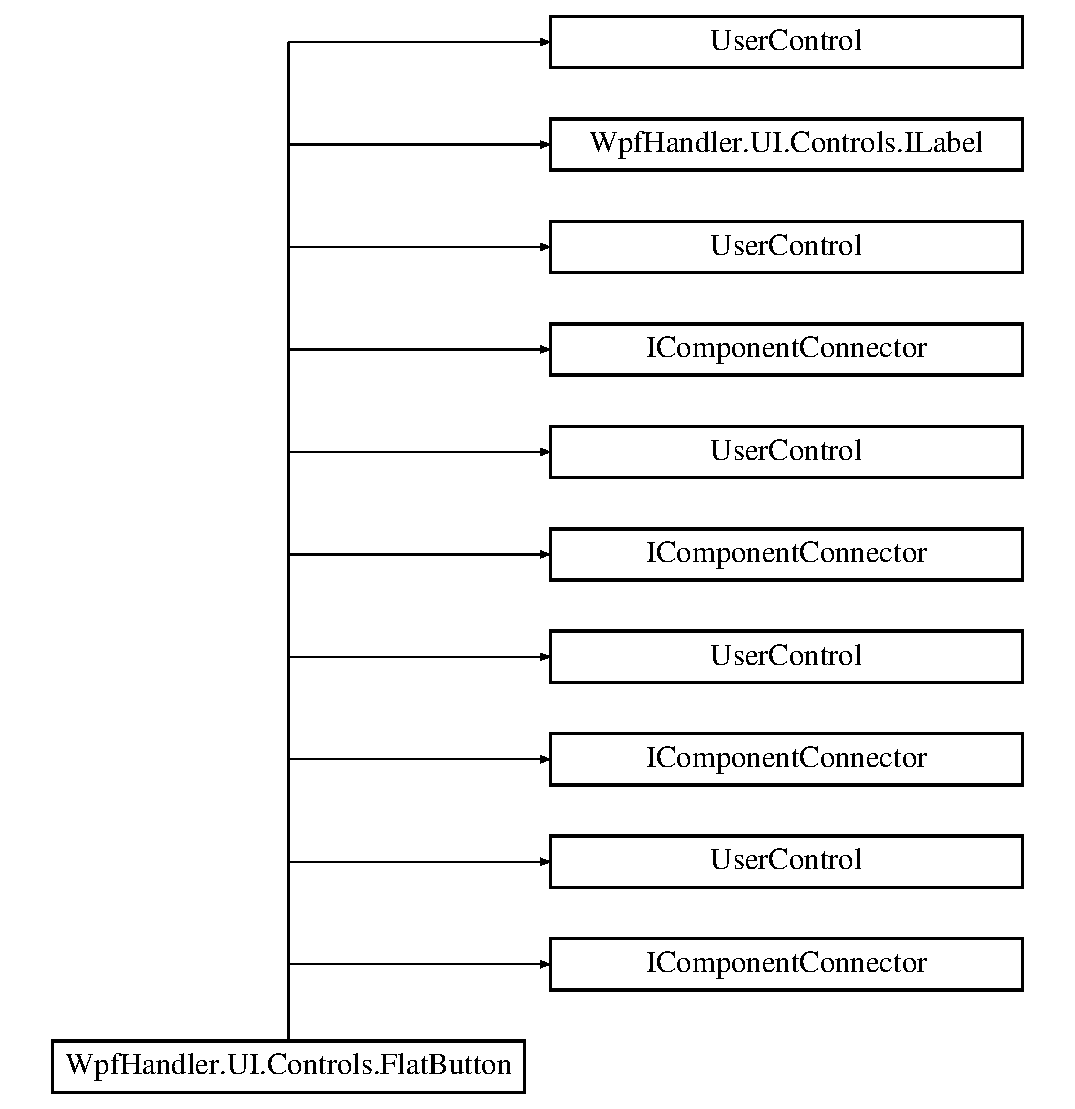
\includegraphics[height=11.000000cm]{d0/d83/class_wpf_handler_1_1_u_i_1_1_controls_1_1_flat_button}
\end{center}
\end{figure}
\subsection*{Public Member Functions}
\begin{DoxyCompactItemize}
\item 
void \mbox{\hyperlink{class_wpf_handler_1_1_u_i_1_1_controls_1_1_flat_button_acabdb68bfd2ca1a7baf68aeb819a7721}{Initialize\+Component}} ()
\begin{DoxyCompactList}\small\item\em Initialize\+Component \end{DoxyCompactList}\item 
void \mbox{\hyperlink{class_wpf_handler_1_1_u_i_1_1_controls_1_1_flat_button_acabdb68bfd2ca1a7baf68aeb819a7721}{Initialize\+Component}} ()
\begin{DoxyCompactList}\small\item\em Initialize\+Component \end{DoxyCompactList}\item 
void \mbox{\hyperlink{class_wpf_handler_1_1_u_i_1_1_controls_1_1_flat_button_acabdb68bfd2ca1a7baf68aeb819a7721}{Initialize\+Component}} ()
\begin{DoxyCompactList}\small\item\em Initialize\+Component \end{DoxyCompactList}\item 
void \mbox{\hyperlink{class_wpf_handler_1_1_u_i_1_1_controls_1_1_flat_button_acabdb68bfd2ca1a7baf68aeb819a7721}{Initialize\+Component}} ()
\begin{DoxyCompactList}\small\item\em Initialize\+Component \end{DoxyCompactList}\item 
\mbox{\hyperlink{class_wpf_handler_1_1_u_i_1_1_controls_1_1_flat_button_a17b78f2f94dad89be055e7bd3eec09da}{Flat\+Button}} ()
\begin{DoxyCompactList}\small\item\em Default constuctor. \end{DoxyCompactList}\end{DoxyCompactItemize}
\subsection*{Static Public Attributes}
\begin{DoxyCompactItemize}
\item 
static readonly Routed\+Event \mbox{\hyperlink{class_wpf_handler_1_1_u_i_1_1_controls_1_1_flat_button_a69190a203535d031a46aa317c5fa93e2}{Click\+Event}}
\begin{DoxyCompactList}\small\item\em Event that will be called when button will be pressed. \end{DoxyCompactList}\item 
static readonly Dependency\+Property \mbox{\hyperlink{class_wpf_handler_1_1_u_i_1_1_controls_1_1_flat_button_acad3d234805ceee99eeced499fe8cd80}{Label\+Property}}
\begin{DoxyCompactList}\small\item\em Bridging X\+A\+ML declaring and the member. \end{DoxyCompactList}\end{DoxyCompactItemize}
\subsection*{Package Attributes}
\begin{DoxyCompactItemize}
\item 
\mbox{\Hypertarget{class_wpf_handler_1_1_u_i_1_1_controls_1_1_flat_button_a26e3853965c8e0f9bc10fe25d4ad54f2}\label{class_wpf_handler_1_1_u_i_1_1_controls_1_1_flat_button_a26e3853965c8e0f9bc10fe25d4ad54f2}} 
\mbox{\hyperlink{class_wpf_handler_1_1_u_i_1_1_controls_1_1_flat_button}{Wpf\+Handler.\+U\+I.\+Controls.\+Flat\+Button}} {\bfseries main}
\item 
\mbox{\Hypertarget{class_wpf_handler_1_1_u_i_1_1_controls_1_1_flat_button_abd241b6a495c587914bde27d925e5fb7}\label{class_wpf_handler_1_1_u_i_1_1_controls_1_1_flat_button_abd241b6a495c587914bde27d925e5fb7}} 
System.\+Windows.\+Controls.\+Button {\bfseries flat\+Button}
\item 
\mbox{\Hypertarget{class_wpf_handler_1_1_u_i_1_1_controls_1_1_flat_button_a40d13fb4b546b97391efb5ae45b621b7}\label{class_wpf_handler_1_1_u_i_1_1_controls_1_1_flat_button_a40d13fb4b546b97391efb5ae45b621b7}} 
System.\+Windows.\+Controls.\+Label {\bfseries label}
\end{DoxyCompactItemize}
\subsection*{Properties}
\begin{DoxyCompactItemize}
\item 
string \mbox{\hyperlink{class_wpf_handler_1_1_u_i_1_1_controls_1_1_flat_button_a2408c739aab8767dd0972dd0a7957abc}{Label}}\hspace{0.3cm}{\ttfamily  \mbox{[}get, set\mbox{]}}
\begin{DoxyCompactList}\small\item\em Text that will be displayed on the button. \end{DoxyCompactList}\item 
Routed\+Event\+Handler \mbox{\hyperlink{class_wpf_handler_1_1_u_i_1_1_controls_1_1_flat_button_ad9184f68d9f9ae9db49fa4a82a97ae15}{Click}}
\begin{DoxyCompactList}\small\item\em Occurs when a \mbox{\hyperlink{class_wpf_handler_1_1_u_i_1_1_controls_1_1_flat_button}{Flat\+Button}}$>$ is clicked. \end{DoxyCompactList}\item 
float \mbox{\hyperlink{class_wpf_handler_1_1_u_i_1_1_controls_1_1_flat_button_ad8f23ebbd9a85097d01940f80d372217}{Label\+Width}}\hspace{0.3cm}{\ttfamily  \mbox{[}get, set\mbox{]}}
\begin{DoxyCompactList}\small\item\em Not supported. \end{DoxyCompactList}\end{DoxyCompactItemize}
\subsection*{Private Member Functions}
\begin{DoxyCompactItemize}
\item 
\mbox{\Hypertarget{class_wpf_handler_1_1_u_i_1_1_controls_1_1_flat_button_a8dbfddaea8859d6d10ddc916cd6ce094}\label{class_wpf_handler_1_1_u_i_1_1_controls_1_1_flat_button_a8dbfddaea8859d6d10ddc916cd6ce094}} 
void System.\+Windows.\+Markup.\+I\+Component\+Connector. {\bfseries Connect} (int connection\+Id, object target)
\item 
\mbox{\Hypertarget{class_wpf_handler_1_1_u_i_1_1_controls_1_1_flat_button_a8dbfddaea8859d6d10ddc916cd6ce094}\label{class_wpf_handler_1_1_u_i_1_1_controls_1_1_flat_button_a8dbfddaea8859d6d10ddc916cd6ce094}} 
void System.\+Windows.\+Markup.\+I\+Component\+Connector. {\bfseries Connect} (int connection\+Id, object target)
\item 
\mbox{\Hypertarget{class_wpf_handler_1_1_u_i_1_1_controls_1_1_flat_button_a8dbfddaea8859d6d10ddc916cd6ce094}\label{class_wpf_handler_1_1_u_i_1_1_controls_1_1_flat_button_a8dbfddaea8859d6d10ddc916cd6ce094}} 
void System.\+Windows.\+Markup.\+I\+Component\+Connector. {\bfseries Connect} (int connection\+Id, object target)
\item 
\mbox{\Hypertarget{class_wpf_handler_1_1_u_i_1_1_controls_1_1_flat_button_a8dbfddaea8859d6d10ddc916cd6ce094}\label{class_wpf_handler_1_1_u_i_1_1_controls_1_1_flat_button_a8dbfddaea8859d6d10ddc916cd6ce094}} 
void System.\+Windows.\+Markup.\+I\+Component\+Connector. {\bfseries Connect} (int connection\+Id, object target)
\item 
void \mbox{\hyperlink{class_wpf_handler_1_1_u_i_1_1_controls_1_1_flat_button_a5248afc0ce1627f03c235fc2d2df8230}{Flat\+Button\+\_\+\+Click}} (object \+\_\+, Routed\+Event\+Args \+\_\+\+\_\+)
\begin{DoxyCompactList}\small\item\em Occurs when internal button clicked. \end{DoxyCompactList}\end{DoxyCompactItemize}
\subsection*{Private Attributes}
\begin{DoxyCompactItemize}
\item 
\mbox{\Hypertarget{class_wpf_handler_1_1_u_i_1_1_controls_1_1_flat_button_a894cd257cfad5ffdf7b4208cb022d41d}\label{class_wpf_handler_1_1_u_i_1_1_controls_1_1_flat_button_a894cd257cfad5ffdf7b4208cb022d41d}} 
bool {\bfseries \+\_\+content\+Loaded}
\end{DoxyCompactItemize}


\subsection{Detailed Description}
\mbox{\hyperlink{class_wpf_handler_1_1_u_i_1_1_controls_1_1_flat_button}{Flat\+Button}} 

Interaction logic for Flat\+Button.\+xaml 

\subsection{Constructor \& Destructor Documentation}
\mbox{\Hypertarget{class_wpf_handler_1_1_u_i_1_1_controls_1_1_flat_button_a17b78f2f94dad89be055e7bd3eec09da}\label{class_wpf_handler_1_1_u_i_1_1_controls_1_1_flat_button_a17b78f2f94dad89be055e7bd3eec09da}} 
\index{Wpf\+Handler\+::\+U\+I\+::\+Controls\+::\+Flat\+Button@{Wpf\+Handler\+::\+U\+I\+::\+Controls\+::\+Flat\+Button}!Flat\+Button@{Flat\+Button}}
\index{Flat\+Button@{Flat\+Button}!Wpf\+Handler\+::\+U\+I\+::\+Controls\+::\+Flat\+Button@{Wpf\+Handler\+::\+U\+I\+::\+Controls\+::\+Flat\+Button}}
\subsubsection{\texorpdfstring{Flat\+Button()}{FlatButton()}}
{\footnotesize\ttfamily Wpf\+Handler.\+U\+I.\+Controls.\+Flat\+Button.\+Flat\+Button (\begin{DoxyParamCaption}{ }\end{DoxyParamCaption})}



Default constuctor. 



\subsection{Member Function Documentation}
\mbox{\Hypertarget{class_wpf_handler_1_1_u_i_1_1_controls_1_1_flat_button_a5248afc0ce1627f03c235fc2d2df8230}\label{class_wpf_handler_1_1_u_i_1_1_controls_1_1_flat_button_a5248afc0ce1627f03c235fc2d2df8230}} 
\index{Wpf\+Handler\+::\+U\+I\+::\+Controls\+::\+Flat\+Button@{Wpf\+Handler\+::\+U\+I\+::\+Controls\+::\+Flat\+Button}!Flat\+Button\+\_\+\+Click@{Flat\+Button\+\_\+\+Click}}
\index{Flat\+Button\+\_\+\+Click@{Flat\+Button\+\_\+\+Click}!Wpf\+Handler\+::\+U\+I\+::\+Controls\+::\+Flat\+Button@{Wpf\+Handler\+::\+U\+I\+::\+Controls\+::\+Flat\+Button}}
\subsubsection{\texorpdfstring{Flat\+Button\+\_\+\+Click()}{FlatButton\_Click()}}
{\footnotesize\ttfamily void Wpf\+Handler.\+U\+I.\+Controls.\+Flat\+Button.\+Flat\+Button\+\_\+\+Click (\begin{DoxyParamCaption}\item[{object}]{\+\_\+,  }\item[{Routed\+Event\+Args}]{\+\_\+\+\_\+ }\end{DoxyParamCaption})\hspace{0.3cm}{\ttfamily [private]}}



Occurs when internal button clicked. 


\begin{DoxyParams}{Parameters}
{\em \+\_\+} & \\
\hline
{\em \+\_\+\+\_\+} & \\
\hline
\end{DoxyParams}
\mbox{\Hypertarget{class_wpf_handler_1_1_u_i_1_1_controls_1_1_flat_button_acabdb68bfd2ca1a7baf68aeb819a7721}\label{class_wpf_handler_1_1_u_i_1_1_controls_1_1_flat_button_acabdb68bfd2ca1a7baf68aeb819a7721}} 
\index{Wpf\+Handler\+::\+U\+I\+::\+Controls\+::\+Flat\+Button@{Wpf\+Handler\+::\+U\+I\+::\+Controls\+::\+Flat\+Button}!Initialize\+Component@{Initialize\+Component}}
\index{Initialize\+Component@{Initialize\+Component}!Wpf\+Handler\+::\+U\+I\+::\+Controls\+::\+Flat\+Button@{Wpf\+Handler\+::\+U\+I\+::\+Controls\+::\+Flat\+Button}}
\subsubsection{\texorpdfstring{Initialize\+Component()}{InitializeComponent()}\hspace{0.1cm}{\footnotesize\ttfamily [1/4]}}
{\footnotesize\ttfamily void Wpf\+Handler.\+U\+I.\+Controls.\+Flat\+Button.\+Initialize\+Component (\begin{DoxyParamCaption}{ }\end{DoxyParamCaption})}



Initialize\+Component 

\mbox{\Hypertarget{class_wpf_handler_1_1_u_i_1_1_controls_1_1_flat_button_acabdb68bfd2ca1a7baf68aeb819a7721}\label{class_wpf_handler_1_1_u_i_1_1_controls_1_1_flat_button_acabdb68bfd2ca1a7baf68aeb819a7721}} 
\index{Wpf\+Handler\+::\+U\+I\+::\+Controls\+::\+Flat\+Button@{Wpf\+Handler\+::\+U\+I\+::\+Controls\+::\+Flat\+Button}!Initialize\+Component@{Initialize\+Component}}
\index{Initialize\+Component@{Initialize\+Component}!Wpf\+Handler\+::\+U\+I\+::\+Controls\+::\+Flat\+Button@{Wpf\+Handler\+::\+U\+I\+::\+Controls\+::\+Flat\+Button}}
\subsubsection{\texorpdfstring{Initialize\+Component()}{InitializeComponent()}\hspace{0.1cm}{\footnotesize\ttfamily [2/4]}}
{\footnotesize\ttfamily void Wpf\+Handler.\+U\+I.\+Controls.\+Flat\+Button.\+Initialize\+Component (\begin{DoxyParamCaption}{ }\end{DoxyParamCaption})}



Initialize\+Component 

\mbox{\Hypertarget{class_wpf_handler_1_1_u_i_1_1_controls_1_1_flat_button_acabdb68bfd2ca1a7baf68aeb819a7721}\label{class_wpf_handler_1_1_u_i_1_1_controls_1_1_flat_button_acabdb68bfd2ca1a7baf68aeb819a7721}} 
\index{Wpf\+Handler\+::\+U\+I\+::\+Controls\+::\+Flat\+Button@{Wpf\+Handler\+::\+U\+I\+::\+Controls\+::\+Flat\+Button}!Initialize\+Component@{Initialize\+Component}}
\index{Initialize\+Component@{Initialize\+Component}!Wpf\+Handler\+::\+U\+I\+::\+Controls\+::\+Flat\+Button@{Wpf\+Handler\+::\+U\+I\+::\+Controls\+::\+Flat\+Button}}
\subsubsection{\texorpdfstring{Initialize\+Component()}{InitializeComponent()}\hspace{0.1cm}{\footnotesize\ttfamily [3/4]}}
{\footnotesize\ttfamily void Wpf\+Handler.\+U\+I.\+Controls.\+Flat\+Button.\+Initialize\+Component (\begin{DoxyParamCaption}{ }\end{DoxyParamCaption})}



Initialize\+Component 

\mbox{\Hypertarget{class_wpf_handler_1_1_u_i_1_1_controls_1_1_flat_button_acabdb68bfd2ca1a7baf68aeb819a7721}\label{class_wpf_handler_1_1_u_i_1_1_controls_1_1_flat_button_acabdb68bfd2ca1a7baf68aeb819a7721}} 
\index{Wpf\+Handler\+::\+U\+I\+::\+Controls\+::\+Flat\+Button@{Wpf\+Handler\+::\+U\+I\+::\+Controls\+::\+Flat\+Button}!Initialize\+Component@{Initialize\+Component}}
\index{Initialize\+Component@{Initialize\+Component}!Wpf\+Handler\+::\+U\+I\+::\+Controls\+::\+Flat\+Button@{Wpf\+Handler\+::\+U\+I\+::\+Controls\+::\+Flat\+Button}}
\subsubsection{\texorpdfstring{Initialize\+Component()}{InitializeComponent()}\hspace{0.1cm}{\footnotesize\ttfamily [4/4]}}
{\footnotesize\ttfamily void Wpf\+Handler.\+U\+I.\+Controls.\+Flat\+Button.\+Initialize\+Component (\begin{DoxyParamCaption}{ }\end{DoxyParamCaption})}



Initialize\+Component 



\subsection{Member Data Documentation}
\mbox{\Hypertarget{class_wpf_handler_1_1_u_i_1_1_controls_1_1_flat_button_a69190a203535d031a46aa317c5fa93e2}\label{class_wpf_handler_1_1_u_i_1_1_controls_1_1_flat_button_a69190a203535d031a46aa317c5fa93e2}} 
\index{Wpf\+Handler\+::\+U\+I\+::\+Controls\+::\+Flat\+Button@{Wpf\+Handler\+::\+U\+I\+::\+Controls\+::\+Flat\+Button}!Click\+Event@{Click\+Event}}
\index{Click\+Event@{Click\+Event}!Wpf\+Handler\+::\+U\+I\+::\+Controls\+::\+Flat\+Button@{Wpf\+Handler\+::\+U\+I\+::\+Controls\+::\+Flat\+Button}}
\subsubsection{\texorpdfstring{Click\+Event}{ClickEvent}}
{\footnotesize\ttfamily readonly Routed\+Event Wpf\+Handler.\+U\+I.\+Controls.\+Flat\+Button.\+Click\+Event\hspace{0.3cm}{\ttfamily [static]}}



Event that will be called when button will be pressed. 

\mbox{\Hypertarget{class_wpf_handler_1_1_u_i_1_1_controls_1_1_flat_button_acad3d234805ceee99eeced499fe8cd80}\label{class_wpf_handler_1_1_u_i_1_1_controls_1_1_flat_button_acad3d234805ceee99eeced499fe8cd80}} 
\index{Wpf\+Handler\+::\+U\+I\+::\+Controls\+::\+Flat\+Button@{Wpf\+Handler\+::\+U\+I\+::\+Controls\+::\+Flat\+Button}!Label\+Property@{Label\+Property}}
\index{Label\+Property@{Label\+Property}!Wpf\+Handler\+::\+U\+I\+::\+Controls\+::\+Flat\+Button@{Wpf\+Handler\+::\+U\+I\+::\+Controls\+::\+Flat\+Button}}
\subsubsection{\texorpdfstring{Label\+Property}{LabelProperty}}
{\footnotesize\ttfamily readonly Dependency\+Property Wpf\+Handler.\+U\+I.\+Controls.\+Flat\+Button.\+Label\+Property\hspace{0.3cm}{\ttfamily [static]}}

{\bfseries Initial value\+:}
\begin{DoxyCode}
= DependencyProperty.Register(
          \textcolor{stringliteral}{"Label"}, typeof(\textcolor{keywordtype}{string}), typeof(FlatButton), \textcolor{keyword}{new} PropertyMetadata(\textcolor{stringliteral}{"Sample"}))
\end{DoxyCode}


Bridging X\+A\+ML declaring and the member. 



\subsection{Property Documentation}
\mbox{\Hypertarget{class_wpf_handler_1_1_u_i_1_1_controls_1_1_flat_button_ad9184f68d9f9ae9db49fa4a82a97ae15}\label{class_wpf_handler_1_1_u_i_1_1_controls_1_1_flat_button_ad9184f68d9f9ae9db49fa4a82a97ae15}} 
\index{Wpf\+Handler\+::\+U\+I\+::\+Controls\+::\+Flat\+Button@{Wpf\+Handler\+::\+U\+I\+::\+Controls\+::\+Flat\+Button}!Click@{Click}}
\index{Click@{Click}!Wpf\+Handler\+::\+U\+I\+::\+Controls\+::\+Flat\+Button@{Wpf\+Handler\+::\+U\+I\+::\+Controls\+::\+Flat\+Button}}
\subsubsection{\texorpdfstring{Click}{Click}}
{\footnotesize\ttfamily Routed\+Event\+Handler Wpf\+Handler.\+U\+I.\+Controls.\+Flat\+Button.\+Click\hspace{0.3cm}{\ttfamily [add]}, {\ttfamily [remove]}}



Occurs when a \mbox{\hyperlink{class_wpf_handler_1_1_u_i_1_1_controls_1_1_flat_button}{Flat\+Button}}$>$ is clicked. 

\mbox{\Hypertarget{class_wpf_handler_1_1_u_i_1_1_controls_1_1_flat_button_a2408c739aab8767dd0972dd0a7957abc}\label{class_wpf_handler_1_1_u_i_1_1_controls_1_1_flat_button_a2408c739aab8767dd0972dd0a7957abc}} 
\index{Wpf\+Handler\+::\+U\+I\+::\+Controls\+::\+Flat\+Button@{Wpf\+Handler\+::\+U\+I\+::\+Controls\+::\+Flat\+Button}!Label@{Label}}
\index{Label@{Label}!Wpf\+Handler\+::\+U\+I\+::\+Controls\+::\+Flat\+Button@{Wpf\+Handler\+::\+U\+I\+::\+Controls\+::\+Flat\+Button}}
\subsubsection{\texorpdfstring{Label}{Label}}
{\footnotesize\ttfamily string Wpf\+Handler.\+U\+I.\+Controls.\+Flat\+Button.\+Label\hspace{0.3cm}{\ttfamily [get]}, {\ttfamily [set]}}



Text that will be displayed on the button. 

\mbox{\Hypertarget{class_wpf_handler_1_1_u_i_1_1_controls_1_1_flat_button_ad8f23ebbd9a85097d01940f80d372217}\label{class_wpf_handler_1_1_u_i_1_1_controls_1_1_flat_button_ad8f23ebbd9a85097d01940f80d372217}} 
\index{Wpf\+Handler\+::\+U\+I\+::\+Controls\+::\+Flat\+Button@{Wpf\+Handler\+::\+U\+I\+::\+Controls\+::\+Flat\+Button}!Label\+Width@{Label\+Width}}
\index{Label\+Width@{Label\+Width}!Wpf\+Handler\+::\+U\+I\+::\+Controls\+::\+Flat\+Button@{Wpf\+Handler\+::\+U\+I\+::\+Controls\+::\+Flat\+Button}}
\subsubsection{\texorpdfstring{Label\+Width}{LabelWidth}}
{\footnotesize\ttfamily float Wpf\+Handler.\+U\+I.\+Controls.\+Flat\+Button.\+Label\+Width\hspace{0.3cm}{\ttfamily [get]}, {\ttfamily [set]}}



Not supported. 



The documentation for this class was generated from the following files\+:\begin{DoxyCompactItemize}
\item 
D\+:/\+Work/\+Git\+Hub/wpf-\/handler/\+Wpf\+Handler/obj/\+Debug/\+U\+I/\+Controls/Flat\+Button.\+g.\+cs\item 
D\+:/\+Work/\+Git\+Hub/wpf-\/handler/\+Wpf\+Handler/obj/\+Debug/\+U\+I/\+Controls/Flat\+Button.\+g.\+i.\+cs\item 
D\+:/\+Work/\+Git\+Hub/wpf-\/handler/\+Wpf\+Handler/\+U\+I/\+Controls/Flat\+Button.\+xaml.\+cs\end{DoxyCompactItemize}

\hypertarget{class_wpf_handler_1_1_u_i_1_1_controls_1_1_flat_password_box}{}\section{Wpf\+Handler.\+U\+I.\+Controls.\+Flat\+Password\+Box Class Reference}
\label{class_wpf_handler_1_1_u_i_1_1_controls_1_1_flat_password_box}\index{Wpf\+Handler.\+U\+I.\+Controls.\+Flat\+Password\+Box@{Wpf\+Handler.\+U\+I.\+Controls.\+Flat\+Password\+Box}}


\mbox{\hyperlink{class_wpf_handler_1_1_u_i_1_1_controls_1_1_flat_password_box}{Flat\+Password\+Box}}  


Inheritance diagram for Wpf\+Handler.\+U\+I.\+Controls.\+Flat\+Password\+Box\+:\begin{figure}[H]
\begin{center}
\leavevmode
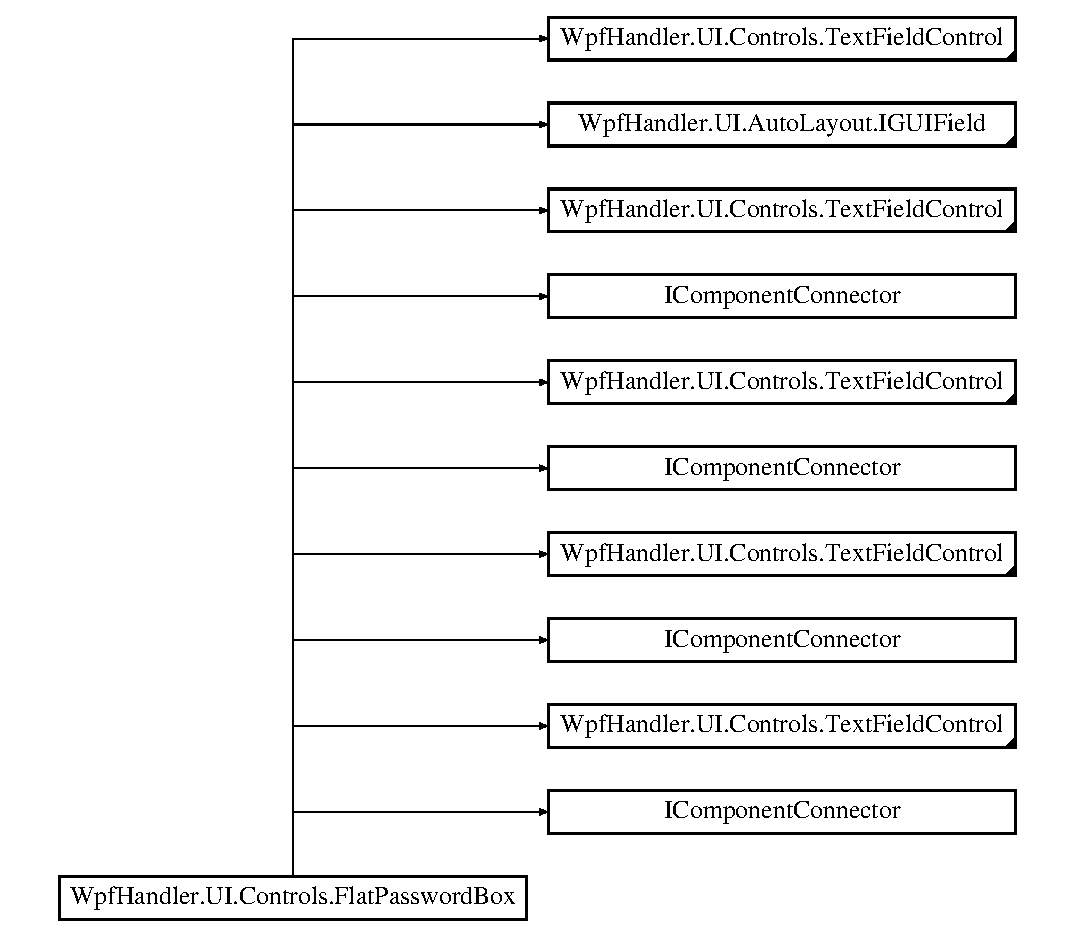
\includegraphics[height=11.000000cm]{d3/d1f/class_wpf_handler_1_1_u_i_1_1_controls_1_1_flat_password_box}
\end{center}
\end{figure}
\subsection*{Public Member Functions}
\begin{DoxyCompactItemize}
\item 
void \mbox{\hyperlink{class_wpf_handler_1_1_u_i_1_1_controls_1_1_flat_password_box_a123fe4c018543ad3c8ed399e9f94b617}{Initialize\+Component}} ()
\begin{DoxyCompactList}\small\item\em Initialize\+Component \end{DoxyCompactList}\item 
void \mbox{\hyperlink{class_wpf_handler_1_1_u_i_1_1_controls_1_1_flat_password_box_a123fe4c018543ad3c8ed399e9f94b617}{Initialize\+Component}} ()
\begin{DoxyCompactList}\small\item\em Initialize\+Component \end{DoxyCompactList}\item 
void \mbox{\hyperlink{class_wpf_handler_1_1_u_i_1_1_controls_1_1_flat_password_box_a123fe4c018543ad3c8ed399e9f94b617}{Initialize\+Component}} ()
\begin{DoxyCompactList}\small\item\em Initialize\+Component \end{DoxyCompactList}\item 
void \mbox{\hyperlink{class_wpf_handler_1_1_u_i_1_1_controls_1_1_flat_password_box_a123fe4c018543ad3c8ed399e9f94b617}{Initialize\+Component}} ()
\begin{DoxyCompactList}\small\item\em Initialize\+Component \end{DoxyCompactList}\item 
\mbox{\hyperlink{class_wpf_handler_1_1_u_i_1_1_controls_1_1_flat_password_box_a9f197f0001f085f6d6e0a0f332793499}{Flat\+Password\+Box}} ()
\begin{DoxyCompactList}\small\item\em Defalut constructor. \end{DoxyCompactList}\item 
void \mbox{\hyperlink{class_wpf_handler_1_1_u_i_1_1_controls_1_1_flat_password_box_a8a06600a127d2b9bc7a1a04767f383e8}{On\+Layout}} (ref \mbox{\hyperlink{class_wpf_handler_1_1_u_i_1_1_auto_layout_1_1_layout_layer}{Layout\+Layer}} layer, params object\mbox{[}$\,$\mbox{]} args)
\begin{DoxyCompactList}\small\item\em Not supported. \end{DoxyCompactList}\item 
override void \mbox{\hyperlink{class_wpf_handler_1_1_u_i_1_1_controls_1_1_flat_password_box_abe285f06393d65f13af4b293f9eb0941}{Recompute\+Layout}} ()
\begin{DoxyCompactList}\small\item\em Recomputing dinamic layout values for providing hight quiality view. \end{DoxyCompactList}\end{DoxyCompactItemize}
\subsection*{Package Functions}
\begin{DoxyCompactItemize}
\item 
\mbox{\Hypertarget{class_wpf_handler_1_1_u_i_1_1_controls_1_1_flat_password_box_a534bc2b9756b39720f896a7b9c105a9b}\label{class_wpf_handler_1_1_u_i_1_1_controls_1_1_flat_password_box_a534bc2b9756b39720f896a7b9c105a9b}} 
System.\+Delegate {\bfseries \+\_\+\+Create\+Delegate} (System.\+Type delegate\+Type, string handler)
\item 
\mbox{\Hypertarget{class_wpf_handler_1_1_u_i_1_1_controls_1_1_flat_password_box_a534bc2b9756b39720f896a7b9c105a9b}\label{class_wpf_handler_1_1_u_i_1_1_controls_1_1_flat_password_box_a534bc2b9756b39720f896a7b9c105a9b}} 
System.\+Delegate {\bfseries \+\_\+\+Create\+Delegate} (System.\+Type delegate\+Type, string handler)
\item 
\mbox{\Hypertarget{class_wpf_handler_1_1_u_i_1_1_controls_1_1_flat_password_box_a534bc2b9756b39720f896a7b9c105a9b}\label{class_wpf_handler_1_1_u_i_1_1_controls_1_1_flat_password_box_a534bc2b9756b39720f896a7b9c105a9b}} 
System.\+Delegate {\bfseries \+\_\+\+Create\+Delegate} (System.\+Type delegate\+Type, string handler)
\item 
\mbox{\Hypertarget{class_wpf_handler_1_1_u_i_1_1_controls_1_1_flat_password_box_a534bc2b9756b39720f896a7b9c105a9b}\label{class_wpf_handler_1_1_u_i_1_1_controls_1_1_flat_password_box_a534bc2b9756b39720f896a7b9c105a9b}} 
System.\+Delegate {\bfseries \+\_\+\+Create\+Delegate} (System.\+Type delegate\+Type, string handler)
\end{DoxyCompactItemize}
\subsection*{Package Attributes}
\begin{DoxyCompactItemize}
\item 
\mbox{\Hypertarget{class_wpf_handler_1_1_u_i_1_1_controls_1_1_flat_password_box_a44b2eb37ff6b536683c63ec5c1b894f9}\label{class_wpf_handler_1_1_u_i_1_1_controls_1_1_flat_password_box_a44b2eb37ff6b536683c63ec5c1b894f9}} 
System.\+Windows.\+Controls.\+Grid {\bfseries flat\+Button}
\item 
\mbox{\Hypertarget{class_wpf_handler_1_1_u_i_1_1_controls_1_1_flat_password_box_a0005bd42a8e3b5b3b8a9bf0777ad2432}\label{class_wpf_handler_1_1_u_i_1_1_controls_1_1_flat_password_box_a0005bd42a8e3b5b3b8a9bf0777ad2432}} 
System.\+Windows.\+Controls.\+Label {\bfseries label\+Element}
\item 
\mbox{\Hypertarget{class_wpf_handler_1_1_u_i_1_1_controls_1_1_flat_password_box_a2528eecafad73e73ff72376b99087c8a}\label{class_wpf_handler_1_1_u_i_1_1_controls_1_1_flat_password_box_a2528eecafad73e73ff72376b99087c8a}} 
System.\+Windows.\+Controls.\+Grid {\bfseries spliter}
\item 
\mbox{\Hypertarget{class_wpf_handler_1_1_u_i_1_1_controls_1_1_flat_password_box_a90d47102a4488676f596b8593f0bdcf2}\label{class_wpf_handler_1_1_u_i_1_1_controls_1_1_flat_password_box_a90d47102a4488676f596b8593f0bdcf2}} 
System.\+Windows.\+Controls.\+Grid {\bfseries field\+Element}
\item 
\mbox{\Hypertarget{class_wpf_handler_1_1_u_i_1_1_controls_1_1_flat_password_box_a633b415dd5950b41ff30666ca00f141a}\label{class_wpf_handler_1_1_u_i_1_1_controls_1_1_flat_password_box_a633b415dd5950b41ff30666ca00f141a}} 
System.\+Windows.\+Controls.\+Password\+Box {\bfseries password\+Box}
\end{DoxyCompactItemize}
\subsection*{Properties}
\begin{DoxyCompactItemize}
\item 
override string \mbox{\hyperlink{class_wpf_handler_1_1_u_i_1_1_controls_1_1_flat_password_box_a19e04b037d81228d50174d63e1ef30f6}{Text}}\hspace{0.3cm}{\ttfamily  \mbox{[}get, set\mbox{]}}
\begin{DoxyCompactList}\small\item\em Text in textbox. \end{DoxyCompactList}\item 
Member\+Info \mbox{\hyperlink{class_wpf_handler_1_1_u_i_1_1_controls_1_1_flat_password_box_ab26770e33e5faaa79da66a5f12b6ed4c}{Binded\+Member}}\hspace{0.3cm}{\ttfamily  \mbox{[}get, set\mbox{]}}
\begin{DoxyCompactList}\small\item\em Member binded to that element by the auto layout handler. \end{DoxyCompactList}\item 
override Framework\+Element \mbox{\hyperlink{class_wpf_handler_1_1_u_i_1_1_controls_1_1_flat_password_box_a12af7f9b9eff179c7155aa236f7fc234}{Label\+Element}}\hspace{0.3cm}{\ttfamily  \mbox{[}get\mbox{]}}
\begin{DoxyCompactList}\small\item\em Returns reference to the label block of \mbox{\hyperlink{namespace_wpf_handler_1_1_u_i}{UI}} element. \end{DoxyCompactList}\item 
override Framework\+Element \mbox{\hyperlink{class_wpf_handler_1_1_u_i_1_1_controls_1_1_flat_password_box_ae661a35bf58daefd8b0c1dc19faed414}{Field\+Element}}\hspace{0.3cm}{\ttfamily  \mbox{[}get\mbox{]}}
\begin{DoxyCompactList}\small\item\em Returns reference to the field block of \mbox{\hyperlink{namespace_wpf_handler_1_1_u_i}{UI}} element. \end{DoxyCompactList}\end{DoxyCompactItemize}
\subsection*{Events}
\begin{DoxyCompactItemize}
\item 
Action$<$ \mbox{\hyperlink{interface_wpf_handler_1_1_u_i_1_1_auto_layout_1_1_i_g_u_i_field}{I\+G\+U\+I\+Field}} $>$ \mbox{\hyperlink{class_wpf_handler_1_1_u_i_1_1_controls_1_1_flat_password_box_a9f85bdb8d3cf805ee1bc3d1d1580c176}{Value\+Changed}}
\begin{DoxyCompactList}\small\item\em Event that will occure in case if value of the field will be changed. Will cause updating of the Binded\+Member value. \end{DoxyCompactList}\end{DoxyCompactItemize}
\subsection*{Private Member Functions}
\begin{DoxyCompactItemize}
\item 
\mbox{\Hypertarget{class_wpf_handler_1_1_u_i_1_1_controls_1_1_flat_password_box_aa1a26564d3ca85c782b1df934f12cd24}\label{class_wpf_handler_1_1_u_i_1_1_controls_1_1_flat_password_box_aa1a26564d3ca85c782b1df934f12cd24}} 
void System.\+Windows.\+Markup.\+I\+Component\+Connector. {\bfseries Connect} (int connection\+Id, object target)
\item 
\mbox{\Hypertarget{class_wpf_handler_1_1_u_i_1_1_controls_1_1_flat_password_box_aa1a26564d3ca85c782b1df934f12cd24}\label{class_wpf_handler_1_1_u_i_1_1_controls_1_1_flat_password_box_aa1a26564d3ca85c782b1df934f12cd24}} 
void System.\+Windows.\+Markup.\+I\+Component\+Connector. {\bfseries Connect} (int connection\+Id, object target)
\item 
\mbox{\Hypertarget{class_wpf_handler_1_1_u_i_1_1_controls_1_1_flat_password_box_aa1a26564d3ca85c782b1df934f12cd24}\label{class_wpf_handler_1_1_u_i_1_1_controls_1_1_flat_password_box_aa1a26564d3ca85c782b1df934f12cd24}} 
void System.\+Windows.\+Markup.\+I\+Component\+Connector. {\bfseries Connect} (int connection\+Id, object target)
\item 
\mbox{\Hypertarget{class_wpf_handler_1_1_u_i_1_1_controls_1_1_flat_password_box_aa1a26564d3ca85c782b1df934f12cd24}\label{class_wpf_handler_1_1_u_i_1_1_controls_1_1_flat_password_box_aa1a26564d3ca85c782b1df934f12cd24}} 
void System.\+Windows.\+Markup.\+I\+Component\+Connector. {\bfseries Connect} (int connection\+Id, object target)
\item 
void \mbox{\hyperlink{class_wpf_handler_1_1_u_i_1_1_controls_1_1_flat_password_box_a617fc7b1bc409502029cffd2b3c53d36}{Password\+Box\+\_\+\+Password\+Changed}} (object sender, Routed\+Event\+Args e)
\begin{DoxyCompactList}\small\item\em Callback that will occure when password will changed. \end{DoxyCompactList}\end{DoxyCompactItemize}
\subsection*{Private Attributes}
\begin{DoxyCompactItemize}
\item 
\mbox{\Hypertarget{class_wpf_handler_1_1_u_i_1_1_controls_1_1_flat_password_box_aeb6fb2434a8bb98dd12230ccd58c59da}\label{class_wpf_handler_1_1_u_i_1_1_controls_1_1_flat_password_box_aeb6fb2434a8bb98dd12230ccd58c59da}} 
bool {\bfseries \+\_\+content\+Loaded}
\end{DoxyCompactItemize}
\subsection*{Additional Inherited Members}


\subsection{Detailed Description}
\mbox{\hyperlink{class_wpf_handler_1_1_u_i_1_1_controls_1_1_flat_password_box}{Flat\+Password\+Box}} 

Interaction logic for Flat\+Password\+Box.\+xaml 

\subsection{Constructor \& Destructor Documentation}
\mbox{\Hypertarget{class_wpf_handler_1_1_u_i_1_1_controls_1_1_flat_password_box_a9f197f0001f085f6d6e0a0f332793499}\label{class_wpf_handler_1_1_u_i_1_1_controls_1_1_flat_password_box_a9f197f0001f085f6d6e0a0f332793499}} 
\index{Wpf\+Handler\+::\+U\+I\+::\+Controls\+::\+Flat\+Password\+Box@{Wpf\+Handler\+::\+U\+I\+::\+Controls\+::\+Flat\+Password\+Box}!Flat\+Password\+Box@{Flat\+Password\+Box}}
\index{Flat\+Password\+Box@{Flat\+Password\+Box}!Wpf\+Handler\+::\+U\+I\+::\+Controls\+::\+Flat\+Password\+Box@{Wpf\+Handler\+::\+U\+I\+::\+Controls\+::\+Flat\+Password\+Box}}
\subsubsection{\texorpdfstring{Flat\+Password\+Box()}{FlatPasswordBox()}}
{\footnotesize\ttfamily Wpf\+Handler.\+U\+I.\+Controls.\+Flat\+Password\+Box.\+Flat\+Password\+Box (\begin{DoxyParamCaption}{ }\end{DoxyParamCaption})}



Defalut constructor. 

Trying to load {\ttfamily \mbox{\hyperlink{class_wpf_handler_1_1_u_i_1_1_controls_1_1_flat_password_box}{Flat\+Password\+Box}}} as  resource. 

\subsection{Member Function Documentation}
\mbox{\Hypertarget{class_wpf_handler_1_1_u_i_1_1_controls_1_1_flat_password_box_a123fe4c018543ad3c8ed399e9f94b617}\label{class_wpf_handler_1_1_u_i_1_1_controls_1_1_flat_password_box_a123fe4c018543ad3c8ed399e9f94b617}} 
\index{Wpf\+Handler\+::\+U\+I\+::\+Controls\+::\+Flat\+Password\+Box@{Wpf\+Handler\+::\+U\+I\+::\+Controls\+::\+Flat\+Password\+Box}!Initialize\+Component@{Initialize\+Component}}
\index{Initialize\+Component@{Initialize\+Component}!Wpf\+Handler\+::\+U\+I\+::\+Controls\+::\+Flat\+Password\+Box@{Wpf\+Handler\+::\+U\+I\+::\+Controls\+::\+Flat\+Password\+Box}}
\subsubsection{\texorpdfstring{Initialize\+Component()}{InitializeComponent()}\hspace{0.1cm}{\footnotesize\ttfamily [1/4]}}
{\footnotesize\ttfamily void Wpf\+Handler.\+U\+I.\+Controls.\+Flat\+Password\+Box.\+Initialize\+Component (\begin{DoxyParamCaption}{ }\end{DoxyParamCaption})}



Initialize\+Component 

\mbox{\Hypertarget{class_wpf_handler_1_1_u_i_1_1_controls_1_1_flat_password_box_a123fe4c018543ad3c8ed399e9f94b617}\label{class_wpf_handler_1_1_u_i_1_1_controls_1_1_flat_password_box_a123fe4c018543ad3c8ed399e9f94b617}} 
\index{Wpf\+Handler\+::\+U\+I\+::\+Controls\+::\+Flat\+Password\+Box@{Wpf\+Handler\+::\+U\+I\+::\+Controls\+::\+Flat\+Password\+Box}!Initialize\+Component@{Initialize\+Component}}
\index{Initialize\+Component@{Initialize\+Component}!Wpf\+Handler\+::\+U\+I\+::\+Controls\+::\+Flat\+Password\+Box@{Wpf\+Handler\+::\+U\+I\+::\+Controls\+::\+Flat\+Password\+Box}}
\subsubsection{\texorpdfstring{Initialize\+Component()}{InitializeComponent()}\hspace{0.1cm}{\footnotesize\ttfamily [2/4]}}
{\footnotesize\ttfamily void Wpf\+Handler.\+U\+I.\+Controls.\+Flat\+Password\+Box.\+Initialize\+Component (\begin{DoxyParamCaption}{ }\end{DoxyParamCaption})}



Initialize\+Component 

\mbox{\Hypertarget{class_wpf_handler_1_1_u_i_1_1_controls_1_1_flat_password_box_a123fe4c018543ad3c8ed399e9f94b617}\label{class_wpf_handler_1_1_u_i_1_1_controls_1_1_flat_password_box_a123fe4c018543ad3c8ed399e9f94b617}} 
\index{Wpf\+Handler\+::\+U\+I\+::\+Controls\+::\+Flat\+Password\+Box@{Wpf\+Handler\+::\+U\+I\+::\+Controls\+::\+Flat\+Password\+Box}!Initialize\+Component@{Initialize\+Component}}
\index{Initialize\+Component@{Initialize\+Component}!Wpf\+Handler\+::\+U\+I\+::\+Controls\+::\+Flat\+Password\+Box@{Wpf\+Handler\+::\+U\+I\+::\+Controls\+::\+Flat\+Password\+Box}}
\subsubsection{\texorpdfstring{Initialize\+Component()}{InitializeComponent()}\hspace{0.1cm}{\footnotesize\ttfamily [3/4]}}
{\footnotesize\ttfamily void Wpf\+Handler.\+U\+I.\+Controls.\+Flat\+Password\+Box.\+Initialize\+Component (\begin{DoxyParamCaption}{ }\end{DoxyParamCaption})}



Initialize\+Component 

\mbox{\Hypertarget{class_wpf_handler_1_1_u_i_1_1_controls_1_1_flat_password_box_a123fe4c018543ad3c8ed399e9f94b617}\label{class_wpf_handler_1_1_u_i_1_1_controls_1_1_flat_password_box_a123fe4c018543ad3c8ed399e9f94b617}} 
\index{Wpf\+Handler\+::\+U\+I\+::\+Controls\+::\+Flat\+Password\+Box@{Wpf\+Handler\+::\+U\+I\+::\+Controls\+::\+Flat\+Password\+Box}!Initialize\+Component@{Initialize\+Component}}
\index{Initialize\+Component@{Initialize\+Component}!Wpf\+Handler\+::\+U\+I\+::\+Controls\+::\+Flat\+Password\+Box@{Wpf\+Handler\+::\+U\+I\+::\+Controls\+::\+Flat\+Password\+Box}}
\subsubsection{\texorpdfstring{Initialize\+Component()}{InitializeComponent()}\hspace{0.1cm}{\footnotesize\ttfamily [4/4]}}
{\footnotesize\ttfamily void Wpf\+Handler.\+U\+I.\+Controls.\+Flat\+Password\+Box.\+Initialize\+Component (\begin{DoxyParamCaption}{ }\end{DoxyParamCaption})}



Initialize\+Component 

\mbox{\Hypertarget{class_wpf_handler_1_1_u_i_1_1_controls_1_1_flat_password_box_a8a06600a127d2b9bc7a1a04767f383e8}\label{class_wpf_handler_1_1_u_i_1_1_controls_1_1_flat_password_box_a8a06600a127d2b9bc7a1a04767f383e8}} 
\index{Wpf\+Handler\+::\+U\+I\+::\+Controls\+::\+Flat\+Password\+Box@{Wpf\+Handler\+::\+U\+I\+::\+Controls\+::\+Flat\+Password\+Box}!On\+Layout@{On\+Layout}}
\index{On\+Layout@{On\+Layout}!Wpf\+Handler\+::\+U\+I\+::\+Controls\+::\+Flat\+Password\+Box@{Wpf\+Handler\+::\+U\+I\+::\+Controls\+::\+Flat\+Password\+Box}}
\subsubsection{\texorpdfstring{On\+Layout()}{OnLayout()}}
{\footnotesize\ttfamily void Wpf\+Handler.\+U\+I.\+Controls.\+Flat\+Password\+Box.\+On\+Layout (\begin{DoxyParamCaption}\item[{ref \mbox{\hyperlink{class_wpf_handler_1_1_u_i_1_1_auto_layout_1_1_layout_layer}{Layout\+Layer}}}]{layer,  }\item[{params object \mbox{[}$\,$\mbox{]}}]{args }\end{DoxyParamCaption})}



Not supported. 


\begin{DoxyParams}{Parameters}
{\em layer} & \\
\hline
{\em args} & \\
\hline
\end{DoxyParams}


Implements \mbox{\hyperlink{interface_wpf_handler_1_1_u_i_1_1_auto_layout_1_1_i_g_u_i_element_a0ff16956f8e8187d51e1b36b6b9f894e}{Wpf\+Handler.\+U\+I.\+Auto\+Layout.\+I\+G\+U\+I\+Element}}.

\mbox{\Hypertarget{class_wpf_handler_1_1_u_i_1_1_controls_1_1_flat_password_box_a617fc7b1bc409502029cffd2b3c53d36}\label{class_wpf_handler_1_1_u_i_1_1_controls_1_1_flat_password_box_a617fc7b1bc409502029cffd2b3c53d36}} 
\index{Wpf\+Handler\+::\+U\+I\+::\+Controls\+::\+Flat\+Password\+Box@{Wpf\+Handler\+::\+U\+I\+::\+Controls\+::\+Flat\+Password\+Box}!Password\+Box\+\_\+\+Password\+Changed@{Password\+Box\+\_\+\+Password\+Changed}}
\index{Password\+Box\+\_\+\+Password\+Changed@{Password\+Box\+\_\+\+Password\+Changed}!Wpf\+Handler\+::\+U\+I\+::\+Controls\+::\+Flat\+Password\+Box@{Wpf\+Handler\+::\+U\+I\+::\+Controls\+::\+Flat\+Password\+Box}}
\subsubsection{\texorpdfstring{Password\+Box\+\_\+\+Password\+Changed()}{PasswordBox\_PasswordChanged()}}
{\footnotesize\ttfamily void Wpf\+Handler.\+U\+I.\+Controls.\+Flat\+Password\+Box.\+Password\+Box\+\_\+\+Password\+Changed (\begin{DoxyParamCaption}\item[{object}]{sender,  }\item[{Routed\+Event\+Args}]{e }\end{DoxyParamCaption})\hspace{0.3cm}{\ttfamily [private]}}



Callback that will occure when password will changed. 


\begin{DoxyParams}{Parameters}
{\em sender} & \\
\hline
{\em e} & \\
\hline
\end{DoxyParams}
\mbox{\Hypertarget{class_wpf_handler_1_1_u_i_1_1_controls_1_1_flat_password_box_abe285f06393d65f13af4b293f9eb0941}\label{class_wpf_handler_1_1_u_i_1_1_controls_1_1_flat_password_box_abe285f06393d65f13af4b293f9eb0941}} 
\index{Wpf\+Handler\+::\+U\+I\+::\+Controls\+::\+Flat\+Password\+Box@{Wpf\+Handler\+::\+U\+I\+::\+Controls\+::\+Flat\+Password\+Box}!Recompute\+Layout@{Recompute\+Layout}}
\index{Recompute\+Layout@{Recompute\+Layout}!Wpf\+Handler\+::\+U\+I\+::\+Controls\+::\+Flat\+Password\+Box@{Wpf\+Handler\+::\+U\+I\+::\+Controls\+::\+Flat\+Password\+Box}}
\subsubsection{\texorpdfstring{Recompute\+Layout()}{RecomputeLayout()}}
{\footnotesize\ttfamily override void Wpf\+Handler.\+U\+I.\+Controls.\+Flat\+Password\+Box.\+Recompute\+Layout (\begin{DoxyParamCaption}{ }\end{DoxyParamCaption})\hspace{0.3cm}{\ttfamily [virtual]}}



Recomputing dinamic layout values for providing hight quiality view. 



Reimplemented from \mbox{\hyperlink{class_wpf_handler_1_1_u_i_1_1_controls_1_1_text_field_control_aaf6c7c81a06ea18f7fd0b709fb9f26b3}{Wpf\+Handler.\+U\+I.\+Controls.\+Text\+Field\+Control}}.



\subsection{Property Documentation}
\mbox{\Hypertarget{class_wpf_handler_1_1_u_i_1_1_controls_1_1_flat_password_box_ab26770e33e5faaa79da66a5f12b6ed4c}\label{class_wpf_handler_1_1_u_i_1_1_controls_1_1_flat_password_box_ab26770e33e5faaa79da66a5f12b6ed4c}} 
\index{Wpf\+Handler\+::\+U\+I\+::\+Controls\+::\+Flat\+Password\+Box@{Wpf\+Handler\+::\+U\+I\+::\+Controls\+::\+Flat\+Password\+Box}!Binded\+Member@{Binded\+Member}}
\index{Binded\+Member@{Binded\+Member}!Wpf\+Handler\+::\+U\+I\+::\+Controls\+::\+Flat\+Password\+Box@{Wpf\+Handler\+::\+U\+I\+::\+Controls\+::\+Flat\+Password\+Box}}
\subsubsection{\texorpdfstring{Binded\+Member}{BindedMember}}
{\footnotesize\ttfamily Member\+Info Wpf\+Handler.\+U\+I.\+Controls.\+Flat\+Password\+Box.\+Binded\+Member\hspace{0.3cm}{\ttfamily [get]}, {\ttfamily [set]}}



Member binded to that element by the auto layout handler. 

\mbox{\Hypertarget{class_wpf_handler_1_1_u_i_1_1_controls_1_1_flat_password_box_ae661a35bf58daefd8b0c1dc19faed414}\label{class_wpf_handler_1_1_u_i_1_1_controls_1_1_flat_password_box_ae661a35bf58daefd8b0c1dc19faed414}} 
\index{Wpf\+Handler\+::\+U\+I\+::\+Controls\+::\+Flat\+Password\+Box@{Wpf\+Handler\+::\+U\+I\+::\+Controls\+::\+Flat\+Password\+Box}!Field\+Element@{Field\+Element}}
\index{Field\+Element@{Field\+Element}!Wpf\+Handler\+::\+U\+I\+::\+Controls\+::\+Flat\+Password\+Box@{Wpf\+Handler\+::\+U\+I\+::\+Controls\+::\+Flat\+Password\+Box}}
\subsubsection{\texorpdfstring{Field\+Element}{FieldElement}}
{\footnotesize\ttfamily override Framework\+Element Wpf\+Handler.\+U\+I.\+Controls.\+Flat\+Password\+Box.\+Field\+Element\hspace{0.3cm}{\ttfamily [get]}}



Returns reference to the field block of \mbox{\hyperlink{namespace_wpf_handler_1_1_u_i}{UI}} element. 

\mbox{\Hypertarget{class_wpf_handler_1_1_u_i_1_1_controls_1_1_flat_password_box_a12af7f9b9eff179c7155aa236f7fc234}\label{class_wpf_handler_1_1_u_i_1_1_controls_1_1_flat_password_box_a12af7f9b9eff179c7155aa236f7fc234}} 
\index{Wpf\+Handler\+::\+U\+I\+::\+Controls\+::\+Flat\+Password\+Box@{Wpf\+Handler\+::\+U\+I\+::\+Controls\+::\+Flat\+Password\+Box}!Label\+Element@{Label\+Element}}
\index{Label\+Element@{Label\+Element}!Wpf\+Handler\+::\+U\+I\+::\+Controls\+::\+Flat\+Password\+Box@{Wpf\+Handler\+::\+U\+I\+::\+Controls\+::\+Flat\+Password\+Box}}
\subsubsection{\texorpdfstring{Label\+Element}{LabelElement}}
{\footnotesize\ttfamily override Framework\+Element Wpf\+Handler.\+U\+I.\+Controls.\+Flat\+Password\+Box.\+Label\+Element\hspace{0.3cm}{\ttfamily [get]}}



Returns reference to the label block of \mbox{\hyperlink{namespace_wpf_handler_1_1_u_i}{UI}} element. 

\mbox{\Hypertarget{class_wpf_handler_1_1_u_i_1_1_controls_1_1_flat_password_box_a19e04b037d81228d50174d63e1ef30f6}\label{class_wpf_handler_1_1_u_i_1_1_controls_1_1_flat_password_box_a19e04b037d81228d50174d63e1ef30f6}} 
\index{Wpf\+Handler\+::\+U\+I\+::\+Controls\+::\+Flat\+Password\+Box@{Wpf\+Handler\+::\+U\+I\+::\+Controls\+::\+Flat\+Password\+Box}!Text@{Text}}
\index{Text@{Text}!Wpf\+Handler\+::\+U\+I\+::\+Controls\+::\+Flat\+Password\+Box@{Wpf\+Handler\+::\+U\+I\+::\+Controls\+::\+Flat\+Password\+Box}}
\subsubsection{\texorpdfstring{Text}{Text}}
{\footnotesize\ttfamily override string Wpf\+Handler.\+U\+I.\+Controls.\+Flat\+Password\+Box.\+Text\hspace{0.3cm}{\ttfamily [get]}, {\ttfamily [set]}}



Text in textbox. 



\subsection{Event Documentation}
\mbox{\Hypertarget{class_wpf_handler_1_1_u_i_1_1_controls_1_1_flat_password_box_a9f85bdb8d3cf805ee1bc3d1d1580c176}\label{class_wpf_handler_1_1_u_i_1_1_controls_1_1_flat_password_box_a9f85bdb8d3cf805ee1bc3d1d1580c176}} 
\index{Wpf\+Handler\+::\+U\+I\+::\+Controls\+::\+Flat\+Password\+Box@{Wpf\+Handler\+::\+U\+I\+::\+Controls\+::\+Flat\+Password\+Box}!Value\+Changed@{Value\+Changed}}
\index{Value\+Changed@{Value\+Changed}!Wpf\+Handler\+::\+U\+I\+::\+Controls\+::\+Flat\+Password\+Box@{Wpf\+Handler\+::\+U\+I\+::\+Controls\+::\+Flat\+Password\+Box}}
\subsubsection{\texorpdfstring{Value\+Changed}{ValueChanged}}
{\footnotesize\ttfamily Action$<$\mbox{\hyperlink{interface_wpf_handler_1_1_u_i_1_1_auto_layout_1_1_i_g_u_i_field}{I\+G\+U\+I\+Field}}$>$ Wpf\+Handler.\+U\+I.\+Controls.\+Flat\+Password\+Box.\+Value\+Changed}



Event that will occure in case if value of the field will be changed. Will cause updating of the Binded\+Member value. 



The documentation for this class was generated from the following files\+:\begin{DoxyCompactItemize}
\item 
D\+:/\+Work/\+Git\+Hub/wpf-\/handler/\+Wpf\+Handler/obj/\+Debug/\+U\+I/\+Controls/Flat\+Password\+Box.\+g.\+cs\item 
D\+:/\+Work/\+Git\+Hub/wpf-\/handler/\+Wpf\+Handler/obj/\+Debug/\+U\+I/\+Controls/Flat\+Password\+Box.\+g.\+i.\+cs\item 
D\+:/\+Work/\+Git\+Hub/wpf-\/handler/\+Wpf\+Handler/\+U\+I/\+Controls/Flat\+Password\+Box.\+xaml.\+cs\end{DoxyCompactItemize}

\hypertarget{class_wpf_handler_1_1_u_i_1_1_controls_1_1_flat_text_box}{}\section{Wpf\+Handler.\+U\+I.\+Controls.\+Flat\+Text\+Box Class Reference}
\label{class_wpf_handler_1_1_u_i_1_1_controls_1_1_flat_text_box}\index{Wpf\+Handler.\+U\+I.\+Controls.\+Flat\+Text\+Box@{Wpf\+Handler.\+U\+I.\+Controls.\+Flat\+Text\+Box}}


\mbox{\hyperlink{class_wpf_handler_1_1_u_i_1_1_controls_1_1_flat_text_box}{Flat\+Text\+Box}}  


Inheritance diagram for Wpf\+Handler.\+U\+I.\+Controls.\+Flat\+Text\+Box\+:\begin{figure}[H]
\begin{center}
\leavevmode
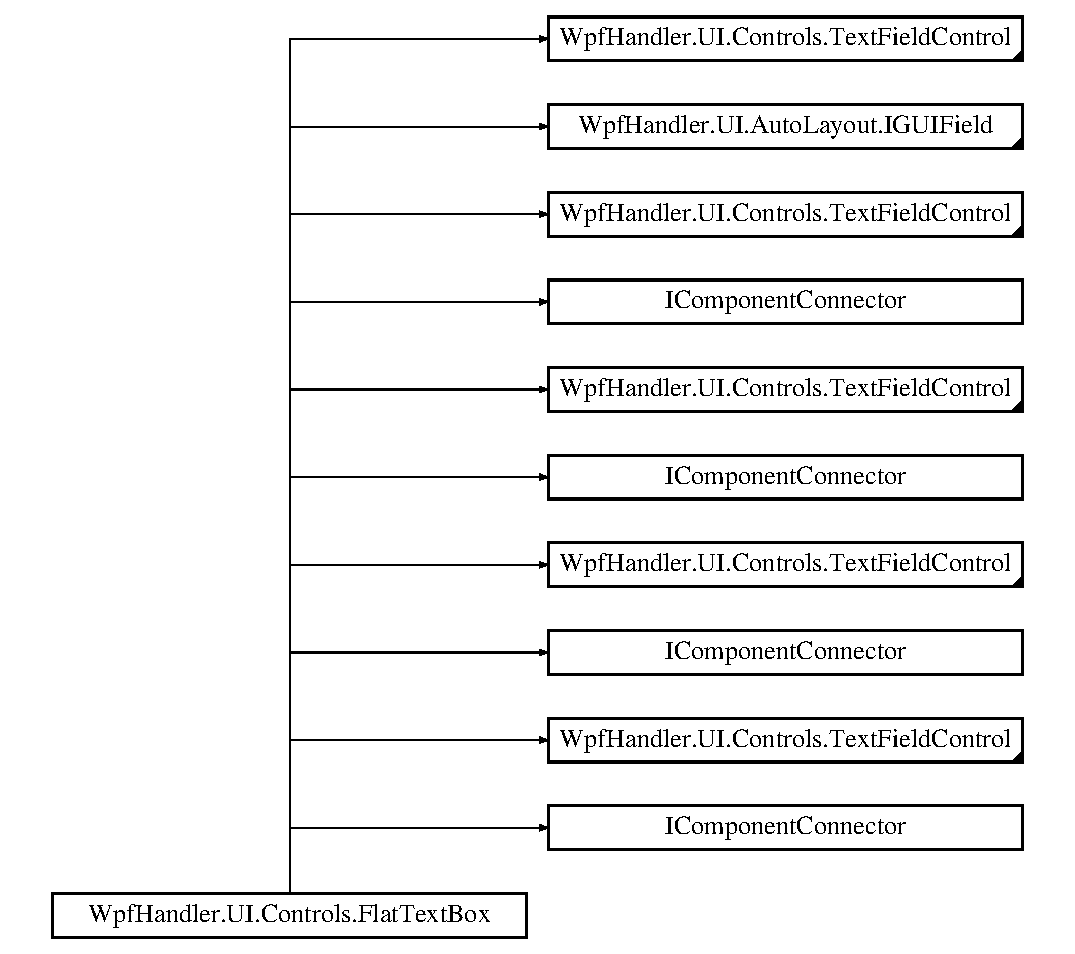
\includegraphics[height=11.000000cm]{d3/d32/class_wpf_handler_1_1_u_i_1_1_controls_1_1_flat_text_box}
\end{center}
\end{figure}
\subsection*{Public Member Functions}
\begin{DoxyCompactItemize}
\item 
void \mbox{\hyperlink{class_wpf_handler_1_1_u_i_1_1_controls_1_1_flat_text_box_a2f6880285eef90455e25c7f3c7fafa56}{Initialize\+Component}} ()
\begin{DoxyCompactList}\small\item\em Initialize\+Component \end{DoxyCompactList}\item 
void \mbox{\hyperlink{class_wpf_handler_1_1_u_i_1_1_controls_1_1_flat_text_box_a2f6880285eef90455e25c7f3c7fafa56}{Initialize\+Component}} ()
\begin{DoxyCompactList}\small\item\em Initialize\+Component \end{DoxyCompactList}\item 
void \mbox{\hyperlink{class_wpf_handler_1_1_u_i_1_1_controls_1_1_flat_text_box_a2f6880285eef90455e25c7f3c7fafa56}{Initialize\+Component}} ()
\begin{DoxyCompactList}\small\item\em Initialize\+Component \end{DoxyCompactList}\item 
void \mbox{\hyperlink{class_wpf_handler_1_1_u_i_1_1_controls_1_1_flat_text_box_a2f6880285eef90455e25c7f3c7fafa56}{Initialize\+Component}} ()
\begin{DoxyCompactList}\small\item\em Initialize\+Component \end{DoxyCompactList}\item 
\mbox{\hyperlink{class_wpf_handler_1_1_u_i_1_1_controls_1_1_flat_text_box_aefe884a51110f8fc9546ce2c86fcf574}{Flat\+Text\+Box}} ()
\begin{DoxyCompactList}\small\item\em Default constructor. Looking for the {\ttfamily \mbox{\hyperlink{class_wpf_handler_1_1_u_i_1_1_controls_1_1_flat_text_box}{Flat\+Text\+Box}}} Style resource. Use default if not found. \end{DoxyCompactList}\item 
void \mbox{\hyperlink{class_wpf_handler_1_1_u_i_1_1_controls_1_1_flat_text_box_a9885e81c438caeec3448c99796503a71}{On\+Layout}} (ref \mbox{\hyperlink{class_wpf_handler_1_1_u_i_1_1_auto_layout_1_1_layout_layer}{Layout\+Layer}} layer, params object\mbox{[}$\,$\mbox{]} args)
\begin{DoxyCompactList}\small\item\em Configurate G\+UI element and bind it to auto layout handler. \end{DoxyCompactList}\item 
override void \mbox{\hyperlink{class_wpf_handler_1_1_u_i_1_1_controls_1_1_flat_text_box_af96bd0b4244565a1ca7a137d56296cda}{Recompute\+Layout}} ()
\begin{DoxyCompactList}\small\item\em Recomputing dinamic layout values for providing hight quiality view. \end{DoxyCompactList}\end{DoxyCompactItemize}
\subsection*{Package Functions}
\begin{DoxyCompactItemize}
\item 
\mbox{\Hypertarget{class_wpf_handler_1_1_u_i_1_1_controls_1_1_flat_text_box_ad95fca5f96c4d3511458804f21944c87}\label{class_wpf_handler_1_1_u_i_1_1_controls_1_1_flat_text_box_ad95fca5f96c4d3511458804f21944c87}} 
System.\+Delegate {\bfseries \+\_\+\+Create\+Delegate} (System.\+Type delegate\+Type, string handler)
\item 
\mbox{\Hypertarget{class_wpf_handler_1_1_u_i_1_1_controls_1_1_flat_text_box_ad95fca5f96c4d3511458804f21944c87}\label{class_wpf_handler_1_1_u_i_1_1_controls_1_1_flat_text_box_ad95fca5f96c4d3511458804f21944c87}} 
System.\+Delegate {\bfseries \+\_\+\+Create\+Delegate} (System.\+Type delegate\+Type, string handler)
\item 
\mbox{\Hypertarget{class_wpf_handler_1_1_u_i_1_1_controls_1_1_flat_text_box_ad95fca5f96c4d3511458804f21944c87}\label{class_wpf_handler_1_1_u_i_1_1_controls_1_1_flat_text_box_ad95fca5f96c4d3511458804f21944c87}} 
System.\+Delegate {\bfseries \+\_\+\+Create\+Delegate} (System.\+Type delegate\+Type, string handler)
\item 
\mbox{\Hypertarget{class_wpf_handler_1_1_u_i_1_1_controls_1_1_flat_text_box_ad95fca5f96c4d3511458804f21944c87}\label{class_wpf_handler_1_1_u_i_1_1_controls_1_1_flat_text_box_ad95fca5f96c4d3511458804f21944c87}} 
System.\+Delegate {\bfseries \+\_\+\+Create\+Delegate} (System.\+Type delegate\+Type, string handler)
\end{DoxyCompactItemize}
\subsection*{Package Attributes}
\begin{DoxyCompactItemize}
\item 
\mbox{\Hypertarget{class_wpf_handler_1_1_u_i_1_1_controls_1_1_flat_text_box_a7ea61ebd8cd69d3801ba5f64276f3f5f}\label{class_wpf_handler_1_1_u_i_1_1_controls_1_1_flat_text_box_a7ea61ebd8cd69d3801ba5f64276f3f5f}} 
System.\+Windows.\+Controls.\+Grid {\bfseries flat\+Button}
\item 
\mbox{\Hypertarget{class_wpf_handler_1_1_u_i_1_1_controls_1_1_flat_text_box_ae0f74426b54b89a958e66f38ae4b541f}\label{class_wpf_handler_1_1_u_i_1_1_controls_1_1_flat_text_box_ae0f74426b54b89a958e66f38ae4b541f}} 
System.\+Windows.\+Controls.\+Label {\bfseries label\+Element}
\item 
\mbox{\Hypertarget{class_wpf_handler_1_1_u_i_1_1_controls_1_1_flat_text_box_acc82c9a54b01cb28a6f5b33d05d5c037}\label{class_wpf_handler_1_1_u_i_1_1_controls_1_1_flat_text_box_acc82c9a54b01cb28a6f5b33d05d5c037}} 
System.\+Windows.\+Controls.\+Grid {\bfseries spliter}
\item 
\mbox{\Hypertarget{class_wpf_handler_1_1_u_i_1_1_controls_1_1_flat_text_box_a43abbd93f032d9fcf3c3c559fd22aad3}\label{class_wpf_handler_1_1_u_i_1_1_controls_1_1_flat_text_box_a43abbd93f032d9fcf3c3c559fd22aad3}} 
System.\+Windows.\+Controls.\+Grid {\bfseries field\+Element}
\item 
\mbox{\Hypertarget{class_wpf_handler_1_1_u_i_1_1_controls_1_1_flat_text_box_a79af97ca25e12d0454582a1aa8a238bd}\label{class_wpf_handler_1_1_u_i_1_1_controls_1_1_flat_text_box_a79af97ca25e12d0454582a1aa8a238bd}} 
System.\+Windows.\+Controls.\+Text\+Box {\bfseries text\+Box}
\end{DoxyCompactItemize}
\subsection*{Properties}
\begin{DoxyCompactItemize}
\item 
Member\+Info \mbox{\hyperlink{class_wpf_handler_1_1_u_i_1_1_controls_1_1_flat_text_box_ae99e62202c09fb6f5e4ecd452c092ba0}{Binded\+Member}}\hspace{0.3cm}{\ttfamily  \mbox{[}get, set\mbox{]}}
\begin{DoxyCompactList}\small\item\em Memeber that will be used as source for the value into \mbox{\hyperlink{namespace_wpf_handler_1_1_u_i}{UI}}. \end{DoxyCompactList}\item 
override Framework\+Element \mbox{\hyperlink{class_wpf_handler_1_1_u_i_1_1_controls_1_1_flat_text_box_ad48de4d845ba738fe0797c3b63625def}{Label\+Element}}\hspace{0.3cm}{\ttfamily  \mbox{[}get\mbox{]}}
\begin{DoxyCompactList}\small\item\em Returns reference to the label block of \mbox{\hyperlink{namespace_wpf_handler_1_1_u_i}{UI}} element. \end{DoxyCompactList}\item 
override Framework\+Element \mbox{\hyperlink{class_wpf_handler_1_1_u_i_1_1_controls_1_1_flat_text_box_a07aad5ace193dc2627b760a7657c170b}{Field\+Element}}\hspace{0.3cm}{\ttfamily  \mbox{[}get\mbox{]}}
\begin{DoxyCompactList}\small\item\em Returns reference to the field block of \mbox{\hyperlink{namespace_wpf_handler_1_1_u_i}{UI}} element. \end{DoxyCompactList}\end{DoxyCompactItemize}
\subsection*{Events}
\begin{DoxyCompactItemize}
\item 
Action$<$ \mbox{\hyperlink{interface_wpf_handler_1_1_u_i_1_1_auto_layout_1_1_i_g_u_i_field}{I\+G\+U\+I\+Field}} $>$ \mbox{\hyperlink{class_wpf_handler_1_1_u_i_1_1_controls_1_1_flat_text_box_a105a5e83858eda13ef8010240747203e}{Value\+Changed}}
\begin{DoxyCompactList}\small\item\em Event that will occure in case if value of the field will be changed. Will cause updating of the Binded\+Member value. \end{DoxyCompactList}\end{DoxyCompactItemize}
\subsection*{Private Member Functions}
\begin{DoxyCompactItemize}
\item 
\mbox{\Hypertarget{class_wpf_handler_1_1_u_i_1_1_controls_1_1_flat_text_box_a2caba72f3d815ce5a0db0589dfb78400}\label{class_wpf_handler_1_1_u_i_1_1_controls_1_1_flat_text_box_a2caba72f3d815ce5a0db0589dfb78400}} 
void System.\+Windows.\+Markup.\+I\+Component\+Connector. {\bfseries Connect} (int connection\+Id, object target)
\item 
\mbox{\Hypertarget{class_wpf_handler_1_1_u_i_1_1_controls_1_1_flat_text_box_a2caba72f3d815ce5a0db0589dfb78400}\label{class_wpf_handler_1_1_u_i_1_1_controls_1_1_flat_text_box_a2caba72f3d815ce5a0db0589dfb78400}} 
void System.\+Windows.\+Markup.\+I\+Component\+Connector. {\bfseries Connect} (int connection\+Id, object target)
\item 
\mbox{\Hypertarget{class_wpf_handler_1_1_u_i_1_1_controls_1_1_flat_text_box_a2caba72f3d815ce5a0db0589dfb78400}\label{class_wpf_handler_1_1_u_i_1_1_controls_1_1_flat_text_box_a2caba72f3d815ce5a0db0589dfb78400}} 
void System.\+Windows.\+Markup.\+I\+Component\+Connector. {\bfseries Connect} (int connection\+Id, object target)
\item 
\mbox{\Hypertarget{class_wpf_handler_1_1_u_i_1_1_controls_1_1_flat_text_box_a2caba72f3d815ce5a0db0589dfb78400}\label{class_wpf_handler_1_1_u_i_1_1_controls_1_1_flat_text_box_a2caba72f3d815ce5a0db0589dfb78400}} 
void System.\+Windows.\+Markup.\+I\+Component\+Connector. {\bfseries Connect} (int connection\+Id, object target)
\item 
void \mbox{\hyperlink{class_wpf_handler_1_1_u_i_1_1_controls_1_1_flat_text_box_a4f374cedf385d1a3983e02f322a6f684}{Text\+Box\+\_\+\+Text\+Changed}} (object sender, Text\+Changed\+Event\+Args e)
\begin{DoxyCompactList}\small\item\em Will occure when password will be changed. \end{DoxyCompactList}\item 
void \mbox{\hyperlink{class_wpf_handler_1_1_u_i_1_1_controls_1_1_flat_text_box_a1d1990512144a1856294f2cef369d7b7}{Text\+Field\+Control\+\_\+\+Loaded}} (object sender, Routed\+Event\+Args e)
\begin{DoxyCompactList}\small\item\em Init configs when all properties applied. \end{DoxyCompactList}\end{DoxyCompactItemize}
\subsection*{Private Attributes}
\begin{DoxyCompactItemize}
\item 
\mbox{\Hypertarget{class_wpf_handler_1_1_u_i_1_1_controls_1_1_flat_text_box_a5ac3253617414dfd0210d24542359afb}\label{class_wpf_handler_1_1_u_i_1_1_controls_1_1_flat_text_box_a5ac3253617414dfd0210d24542359afb}} 
bool {\bfseries \+\_\+content\+Loaded}
\item 
string \mbox{\hyperlink{class_wpf_handler_1_1_u_i_1_1_controls_1_1_flat_text_box_a749af03c71b6c8f4b0075af04535a03c}{text\+Property\+Bufer}}
\begin{DoxyCompactList}\small\item\em Bufer that contains last valid stored text from textbox. \end{DoxyCompactList}\end{DoxyCompactItemize}
\subsection*{Additional Inherited Members}


\subsection{Detailed Description}
\mbox{\hyperlink{class_wpf_handler_1_1_u_i_1_1_controls_1_1_flat_text_box}{Flat\+Text\+Box}} 

Interaction logic for Flat\+Text\+Box.\+xaml 

\subsection{Constructor \& Destructor Documentation}
\mbox{\Hypertarget{class_wpf_handler_1_1_u_i_1_1_controls_1_1_flat_text_box_aefe884a51110f8fc9546ce2c86fcf574}\label{class_wpf_handler_1_1_u_i_1_1_controls_1_1_flat_text_box_aefe884a51110f8fc9546ce2c86fcf574}} 
\index{Wpf\+Handler\+::\+U\+I\+::\+Controls\+::\+Flat\+Text\+Box@{Wpf\+Handler\+::\+U\+I\+::\+Controls\+::\+Flat\+Text\+Box}!Flat\+Text\+Box@{Flat\+Text\+Box}}
\index{Flat\+Text\+Box@{Flat\+Text\+Box}!Wpf\+Handler\+::\+U\+I\+::\+Controls\+::\+Flat\+Text\+Box@{Wpf\+Handler\+::\+U\+I\+::\+Controls\+::\+Flat\+Text\+Box}}
\subsubsection{\texorpdfstring{Flat\+Text\+Box()}{FlatTextBox()}}
{\footnotesize\ttfamily Wpf\+Handler.\+U\+I.\+Controls.\+Flat\+Text\+Box.\+Flat\+Text\+Box (\begin{DoxyParamCaption}{ }\end{DoxyParamCaption})}



Default constructor. Looking for the {\ttfamily \mbox{\hyperlink{class_wpf_handler_1_1_u_i_1_1_controls_1_1_flat_text_box}{Flat\+Text\+Box}}} Style resource. Use default if not found. 



\subsection{Member Function Documentation}
\mbox{\Hypertarget{class_wpf_handler_1_1_u_i_1_1_controls_1_1_flat_text_box_a2f6880285eef90455e25c7f3c7fafa56}\label{class_wpf_handler_1_1_u_i_1_1_controls_1_1_flat_text_box_a2f6880285eef90455e25c7f3c7fafa56}} 
\index{Wpf\+Handler\+::\+U\+I\+::\+Controls\+::\+Flat\+Text\+Box@{Wpf\+Handler\+::\+U\+I\+::\+Controls\+::\+Flat\+Text\+Box}!Initialize\+Component@{Initialize\+Component}}
\index{Initialize\+Component@{Initialize\+Component}!Wpf\+Handler\+::\+U\+I\+::\+Controls\+::\+Flat\+Text\+Box@{Wpf\+Handler\+::\+U\+I\+::\+Controls\+::\+Flat\+Text\+Box}}
\subsubsection{\texorpdfstring{Initialize\+Component()}{InitializeComponent()}\hspace{0.1cm}{\footnotesize\ttfamily [1/4]}}
{\footnotesize\ttfamily void Wpf\+Handler.\+U\+I.\+Controls.\+Flat\+Text\+Box.\+Initialize\+Component (\begin{DoxyParamCaption}{ }\end{DoxyParamCaption})}



Initialize\+Component 

\mbox{\Hypertarget{class_wpf_handler_1_1_u_i_1_1_controls_1_1_flat_text_box_a2f6880285eef90455e25c7f3c7fafa56}\label{class_wpf_handler_1_1_u_i_1_1_controls_1_1_flat_text_box_a2f6880285eef90455e25c7f3c7fafa56}} 
\index{Wpf\+Handler\+::\+U\+I\+::\+Controls\+::\+Flat\+Text\+Box@{Wpf\+Handler\+::\+U\+I\+::\+Controls\+::\+Flat\+Text\+Box}!Initialize\+Component@{Initialize\+Component}}
\index{Initialize\+Component@{Initialize\+Component}!Wpf\+Handler\+::\+U\+I\+::\+Controls\+::\+Flat\+Text\+Box@{Wpf\+Handler\+::\+U\+I\+::\+Controls\+::\+Flat\+Text\+Box}}
\subsubsection{\texorpdfstring{Initialize\+Component()}{InitializeComponent()}\hspace{0.1cm}{\footnotesize\ttfamily [2/4]}}
{\footnotesize\ttfamily void Wpf\+Handler.\+U\+I.\+Controls.\+Flat\+Text\+Box.\+Initialize\+Component (\begin{DoxyParamCaption}{ }\end{DoxyParamCaption})}



Initialize\+Component 

\mbox{\Hypertarget{class_wpf_handler_1_1_u_i_1_1_controls_1_1_flat_text_box_a2f6880285eef90455e25c7f3c7fafa56}\label{class_wpf_handler_1_1_u_i_1_1_controls_1_1_flat_text_box_a2f6880285eef90455e25c7f3c7fafa56}} 
\index{Wpf\+Handler\+::\+U\+I\+::\+Controls\+::\+Flat\+Text\+Box@{Wpf\+Handler\+::\+U\+I\+::\+Controls\+::\+Flat\+Text\+Box}!Initialize\+Component@{Initialize\+Component}}
\index{Initialize\+Component@{Initialize\+Component}!Wpf\+Handler\+::\+U\+I\+::\+Controls\+::\+Flat\+Text\+Box@{Wpf\+Handler\+::\+U\+I\+::\+Controls\+::\+Flat\+Text\+Box}}
\subsubsection{\texorpdfstring{Initialize\+Component()}{InitializeComponent()}\hspace{0.1cm}{\footnotesize\ttfamily [3/4]}}
{\footnotesize\ttfamily void Wpf\+Handler.\+U\+I.\+Controls.\+Flat\+Text\+Box.\+Initialize\+Component (\begin{DoxyParamCaption}{ }\end{DoxyParamCaption})}



Initialize\+Component 

\mbox{\Hypertarget{class_wpf_handler_1_1_u_i_1_1_controls_1_1_flat_text_box_a2f6880285eef90455e25c7f3c7fafa56}\label{class_wpf_handler_1_1_u_i_1_1_controls_1_1_flat_text_box_a2f6880285eef90455e25c7f3c7fafa56}} 
\index{Wpf\+Handler\+::\+U\+I\+::\+Controls\+::\+Flat\+Text\+Box@{Wpf\+Handler\+::\+U\+I\+::\+Controls\+::\+Flat\+Text\+Box}!Initialize\+Component@{Initialize\+Component}}
\index{Initialize\+Component@{Initialize\+Component}!Wpf\+Handler\+::\+U\+I\+::\+Controls\+::\+Flat\+Text\+Box@{Wpf\+Handler\+::\+U\+I\+::\+Controls\+::\+Flat\+Text\+Box}}
\subsubsection{\texorpdfstring{Initialize\+Component()}{InitializeComponent()}\hspace{0.1cm}{\footnotesize\ttfamily [4/4]}}
{\footnotesize\ttfamily void Wpf\+Handler.\+U\+I.\+Controls.\+Flat\+Text\+Box.\+Initialize\+Component (\begin{DoxyParamCaption}{ }\end{DoxyParamCaption})}



Initialize\+Component 

\mbox{\Hypertarget{class_wpf_handler_1_1_u_i_1_1_controls_1_1_flat_text_box_a9885e81c438caeec3448c99796503a71}\label{class_wpf_handler_1_1_u_i_1_1_controls_1_1_flat_text_box_a9885e81c438caeec3448c99796503a71}} 
\index{Wpf\+Handler\+::\+U\+I\+::\+Controls\+::\+Flat\+Text\+Box@{Wpf\+Handler\+::\+U\+I\+::\+Controls\+::\+Flat\+Text\+Box}!On\+Layout@{On\+Layout}}
\index{On\+Layout@{On\+Layout}!Wpf\+Handler\+::\+U\+I\+::\+Controls\+::\+Flat\+Text\+Box@{Wpf\+Handler\+::\+U\+I\+::\+Controls\+::\+Flat\+Text\+Box}}
\subsubsection{\texorpdfstring{On\+Layout()}{OnLayout()}}
{\footnotesize\ttfamily void Wpf\+Handler.\+U\+I.\+Controls.\+Flat\+Text\+Box.\+On\+Layout (\begin{DoxyParamCaption}\item[{ref \mbox{\hyperlink{class_wpf_handler_1_1_u_i_1_1_auto_layout_1_1_layout_layer}{Layout\+Layer}}}]{layer,  }\item[{params object \mbox{[}$\,$\mbox{]}}]{args }\end{DoxyParamCaption})}



Configurate G\+UI element and bind it to auto layout handler. 


\begin{DoxyParams}{Parameters}
{\em layer} & Target \mbox{\hyperlink{namespace_wpf_handler_1_1_u_i}{UI}} layer.\\
\hline
{\em args} & Must contains\+: U\+I\+Descriptor and Member\+Info\\
\hline
\end{DoxyParams}


Implements \mbox{\hyperlink{interface_wpf_handler_1_1_u_i_1_1_auto_layout_1_1_i_g_u_i_element_a0ff16956f8e8187d51e1b36b6b9f894e}{Wpf\+Handler.\+U\+I.\+Auto\+Layout.\+I\+G\+U\+I\+Element}}.

\mbox{\Hypertarget{class_wpf_handler_1_1_u_i_1_1_controls_1_1_flat_text_box_af96bd0b4244565a1ca7a137d56296cda}\label{class_wpf_handler_1_1_u_i_1_1_controls_1_1_flat_text_box_af96bd0b4244565a1ca7a137d56296cda}} 
\index{Wpf\+Handler\+::\+U\+I\+::\+Controls\+::\+Flat\+Text\+Box@{Wpf\+Handler\+::\+U\+I\+::\+Controls\+::\+Flat\+Text\+Box}!Recompute\+Layout@{Recompute\+Layout}}
\index{Recompute\+Layout@{Recompute\+Layout}!Wpf\+Handler\+::\+U\+I\+::\+Controls\+::\+Flat\+Text\+Box@{Wpf\+Handler\+::\+U\+I\+::\+Controls\+::\+Flat\+Text\+Box}}
\subsubsection{\texorpdfstring{Recompute\+Layout()}{RecomputeLayout()}}
{\footnotesize\ttfamily override void Wpf\+Handler.\+U\+I.\+Controls.\+Flat\+Text\+Box.\+Recompute\+Layout (\begin{DoxyParamCaption}{ }\end{DoxyParamCaption})\hspace{0.3cm}{\ttfamily [virtual]}}



Recomputing dinamic layout values for providing hight quiality view. 



Reimplemented from \mbox{\hyperlink{class_wpf_handler_1_1_u_i_1_1_controls_1_1_text_field_control_aaf6c7c81a06ea18f7fd0b709fb9f26b3}{Wpf\+Handler.\+U\+I.\+Controls.\+Text\+Field\+Control}}.

\mbox{\Hypertarget{class_wpf_handler_1_1_u_i_1_1_controls_1_1_flat_text_box_a4f374cedf385d1a3983e02f322a6f684}\label{class_wpf_handler_1_1_u_i_1_1_controls_1_1_flat_text_box_a4f374cedf385d1a3983e02f322a6f684}} 
\index{Wpf\+Handler\+::\+U\+I\+::\+Controls\+::\+Flat\+Text\+Box@{Wpf\+Handler\+::\+U\+I\+::\+Controls\+::\+Flat\+Text\+Box}!Text\+Box\+\_\+\+Text\+Changed@{Text\+Box\+\_\+\+Text\+Changed}}
\index{Text\+Box\+\_\+\+Text\+Changed@{Text\+Box\+\_\+\+Text\+Changed}!Wpf\+Handler\+::\+U\+I\+::\+Controls\+::\+Flat\+Text\+Box@{Wpf\+Handler\+::\+U\+I\+::\+Controls\+::\+Flat\+Text\+Box}}
\subsubsection{\texorpdfstring{Text\+Box\+\_\+\+Text\+Changed()}{TextBox\_TextChanged()}}
{\footnotesize\ttfamily void Wpf\+Handler.\+U\+I.\+Controls.\+Flat\+Text\+Box.\+Text\+Box\+\_\+\+Text\+Changed (\begin{DoxyParamCaption}\item[{object}]{sender,  }\item[{Text\+Changed\+Event\+Args}]{e }\end{DoxyParamCaption})\hspace{0.3cm}{\ttfamily [private]}}



Will occure when password will be changed. 


\begin{DoxyParams}{Parameters}
{\em sender} & \\
\hline
{\em e} & \\
\hline
\end{DoxyParams}
\mbox{\Hypertarget{class_wpf_handler_1_1_u_i_1_1_controls_1_1_flat_text_box_a1d1990512144a1856294f2cef369d7b7}\label{class_wpf_handler_1_1_u_i_1_1_controls_1_1_flat_text_box_a1d1990512144a1856294f2cef369d7b7}} 
\index{Wpf\+Handler\+::\+U\+I\+::\+Controls\+::\+Flat\+Text\+Box@{Wpf\+Handler\+::\+U\+I\+::\+Controls\+::\+Flat\+Text\+Box}!Text\+Field\+Control\+\_\+\+Loaded@{Text\+Field\+Control\+\_\+\+Loaded}}
\index{Text\+Field\+Control\+\_\+\+Loaded@{Text\+Field\+Control\+\_\+\+Loaded}!Wpf\+Handler\+::\+U\+I\+::\+Controls\+::\+Flat\+Text\+Box@{Wpf\+Handler\+::\+U\+I\+::\+Controls\+::\+Flat\+Text\+Box}}
\subsubsection{\texorpdfstring{Text\+Field\+Control\+\_\+\+Loaded()}{TextFieldControl\_Loaded()}}
{\footnotesize\ttfamily void Wpf\+Handler.\+U\+I.\+Controls.\+Flat\+Text\+Box.\+Text\+Field\+Control\+\_\+\+Loaded (\begin{DoxyParamCaption}\item[{object}]{sender,  }\item[{Routed\+Event\+Args}]{e }\end{DoxyParamCaption})\hspace{0.3cm}{\ttfamily [private]}}



Init configs when all properties applied. 


\begin{DoxyParams}{Parameters}
{\em sender} & \\
\hline
{\em e} & \\
\hline
\end{DoxyParams}


\subsection{Member Data Documentation}
\mbox{\Hypertarget{class_wpf_handler_1_1_u_i_1_1_controls_1_1_flat_text_box_a749af03c71b6c8f4b0075af04535a03c}\label{class_wpf_handler_1_1_u_i_1_1_controls_1_1_flat_text_box_a749af03c71b6c8f4b0075af04535a03c}} 
\index{Wpf\+Handler\+::\+U\+I\+::\+Controls\+::\+Flat\+Text\+Box@{Wpf\+Handler\+::\+U\+I\+::\+Controls\+::\+Flat\+Text\+Box}!text\+Property\+Bufer@{text\+Property\+Bufer}}
\index{text\+Property\+Bufer@{text\+Property\+Bufer}!Wpf\+Handler\+::\+U\+I\+::\+Controls\+::\+Flat\+Text\+Box@{Wpf\+Handler\+::\+U\+I\+::\+Controls\+::\+Flat\+Text\+Box}}
\subsubsection{\texorpdfstring{text\+Property\+Bufer}{textPropertyBufer}}
{\footnotesize\ttfamily string Wpf\+Handler.\+U\+I.\+Controls.\+Flat\+Text\+Box.\+text\+Property\+Bufer\hspace{0.3cm}{\ttfamily [private]}}



Bufer that contains last valid stored text from textbox. 



\subsection{Property Documentation}
\mbox{\Hypertarget{class_wpf_handler_1_1_u_i_1_1_controls_1_1_flat_text_box_ae99e62202c09fb6f5e4ecd452c092ba0}\label{class_wpf_handler_1_1_u_i_1_1_controls_1_1_flat_text_box_ae99e62202c09fb6f5e4ecd452c092ba0}} 
\index{Wpf\+Handler\+::\+U\+I\+::\+Controls\+::\+Flat\+Text\+Box@{Wpf\+Handler\+::\+U\+I\+::\+Controls\+::\+Flat\+Text\+Box}!Binded\+Member@{Binded\+Member}}
\index{Binded\+Member@{Binded\+Member}!Wpf\+Handler\+::\+U\+I\+::\+Controls\+::\+Flat\+Text\+Box@{Wpf\+Handler\+::\+U\+I\+::\+Controls\+::\+Flat\+Text\+Box}}
\subsubsection{\texorpdfstring{Binded\+Member}{BindedMember}}
{\footnotesize\ttfamily Member\+Info Wpf\+Handler.\+U\+I.\+Controls.\+Flat\+Text\+Box.\+Binded\+Member\hspace{0.3cm}{\ttfamily [get]}, {\ttfamily [set]}}



Memeber that will be used as source for the value into \mbox{\hyperlink{namespace_wpf_handler_1_1_u_i}{UI}}. 

\mbox{\Hypertarget{class_wpf_handler_1_1_u_i_1_1_controls_1_1_flat_text_box_a07aad5ace193dc2627b760a7657c170b}\label{class_wpf_handler_1_1_u_i_1_1_controls_1_1_flat_text_box_a07aad5ace193dc2627b760a7657c170b}} 
\index{Wpf\+Handler\+::\+U\+I\+::\+Controls\+::\+Flat\+Text\+Box@{Wpf\+Handler\+::\+U\+I\+::\+Controls\+::\+Flat\+Text\+Box}!Field\+Element@{Field\+Element}}
\index{Field\+Element@{Field\+Element}!Wpf\+Handler\+::\+U\+I\+::\+Controls\+::\+Flat\+Text\+Box@{Wpf\+Handler\+::\+U\+I\+::\+Controls\+::\+Flat\+Text\+Box}}
\subsubsection{\texorpdfstring{Field\+Element}{FieldElement}}
{\footnotesize\ttfamily override Framework\+Element Wpf\+Handler.\+U\+I.\+Controls.\+Flat\+Text\+Box.\+Field\+Element\hspace{0.3cm}{\ttfamily [get]}}



Returns reference to the field block of \mbox{\hyperlink{namespace_wpf_handler_1_1_u_i}{UI}} element. 

\mbox{\Hypertarget{class_wpf_handler_1_1_u_i_1_1_controls_1_1_flat_text_box_ad48de4d845ba738fe0797c3b63625def}\label{class_wpf_handler_1_1_u_i_1_1_controls_1_1_flat_text_box_ad48de4d845ba738fe0797c3b63625def}} 
\index{Wpf\+Handler\+::\+U\+I\+::\+Controls\+::\+Flat\+Text\+Box@{Wpf\+Handler\+::\+U\+I\+::\+Controls\+::\+Flat\+Text\+Box}!Label\+Element@{Label\+Element}}
\index{Label\+Element@{Label\+Element}!Wpf\+Handler\+::\+U\+I\+::\+Controls\+::\+Flat\+Text\+Box@{Wpf\+Handler\+::\+U\+I\+::\+Controls\+::\+Flat\+Text\+Box}}
\subsubsection{\texorpdfstring{Label\+Element}{LabelElement}}
{\footnotesize\ttfamily override Framework\+Element Wpf\+Handler.\+U\+I.\+Controls.\+Flat\+Text\+Box.\+Label\+Element\hspace{0.3cm}{\ttfamily [get]}}



Returns reference to the label block of \mbox{\hyperlink{namespace_wpf_handler_1_1_u_i}{UI}} element. 



\subsection{Event Documentation}
\mbox{\Hypertarget{class_wpf_handler_1_1_u_i_1_1_controls_1_1_flat_text_box_a105a5e83858eda13ef8010240747203e}\label{class_wpf_handler_1_1_u_i_1_1_controls_1_1_flat_text_box_a105a5e83858eda13ef8010240747203e}} 
\index{Wpf\+Handler\+::\+U\+I\+::\+Controls\+::\+Flat\+Text\+Box@{Wpf\+Handler\+::\+U\+I\+::\+Controls\+::\+Flat\+Text\+Box}!Value\+Changed@{Value\+Changed}}
\index{Value\+Changed@{Value\+Changed}!Wpf\+Handler\+::\+U\+I\+::\+Controls\+::\+Flat\+Text\+Box@{Wpf\+Handler\+::\+U\+I\+::\+Controls\+::\+Flat\+Text\+Box}}
\subsubsection{\texorpdfstring{Value\+Changed}{ValueChanged}}
{\footnotesize\ttfamily Action$<$\mbox{\hyperlink{interface_wpf_handler_1_1_u_i_1_1_auto_layout_1_1_i_g_u_i_field}{I\+G\+U\+I\+Field}}$>$ Wpf\+Handler.\+U\+I.\+Controls.\+Flat\+Text\+Box.\+Value\+Changed}



Event that will occure in case if value of the field will be changed. Will cause updating of the Binded\+Member value. 



The documentation for this class was generated from the following files\+:\begin{DoxyCompactItemize}
\item 
D\+:/\+Work/\+Git\+Hub/wpf-\/handler/\+Wpf\+Handler/obj/\+Debug/\+U\+I/\+Controls/Flat\+Text\+Box.\+g.\+cs\item 
D\+:/\+Work/\+Git\+Hub/wpf-\/handler/\+Wpf\+Handler/obj/\+Debug/\+U\+I/\+Controls/Flat\+Text\+Box.\+g.\+i.\+cs\item 
D\+:/\+Work/\+Git\+Hub/wpf-\/handler/\+Wpf\+Handler/\+U\+I/\+Controls/Flat\+Text\+Box.\+xaml.\+cs\end{DoxyCompactItemize}

\hypertarget{class_wpf_handler_1_1_u_i_1_1_controls_1_1_flat_toggles_group}{}\section{Wpf\+Handler.\+U\+I.\+Controls.\+Flat\+Toggles\+Group Class Reference}
\label{class_wpf_handler_1_1_u_i_1_1_controls_1_1_flat_toggles_group}\index{Wpf\+Handler.\+U\+I.\+Controls.\+Flat\+Toggles\+Group@{Wpf\+Handler.\+U\+I.\+Controls.\+Flat\+Toggles\+Group}}


\mbox{\hyperlink{class_wpf_handler_1_1_u_i_1_1_controls_1_1_flat_toggles_group}{Flat\+Toggles\+Group}}  


Inheritance diagram for Wpf\+Handler.\+U\+I.\+Controls.\+Flat\+Toggles\+Group\+:\begin{figure}[H]
\begin{center}
\leavevmode
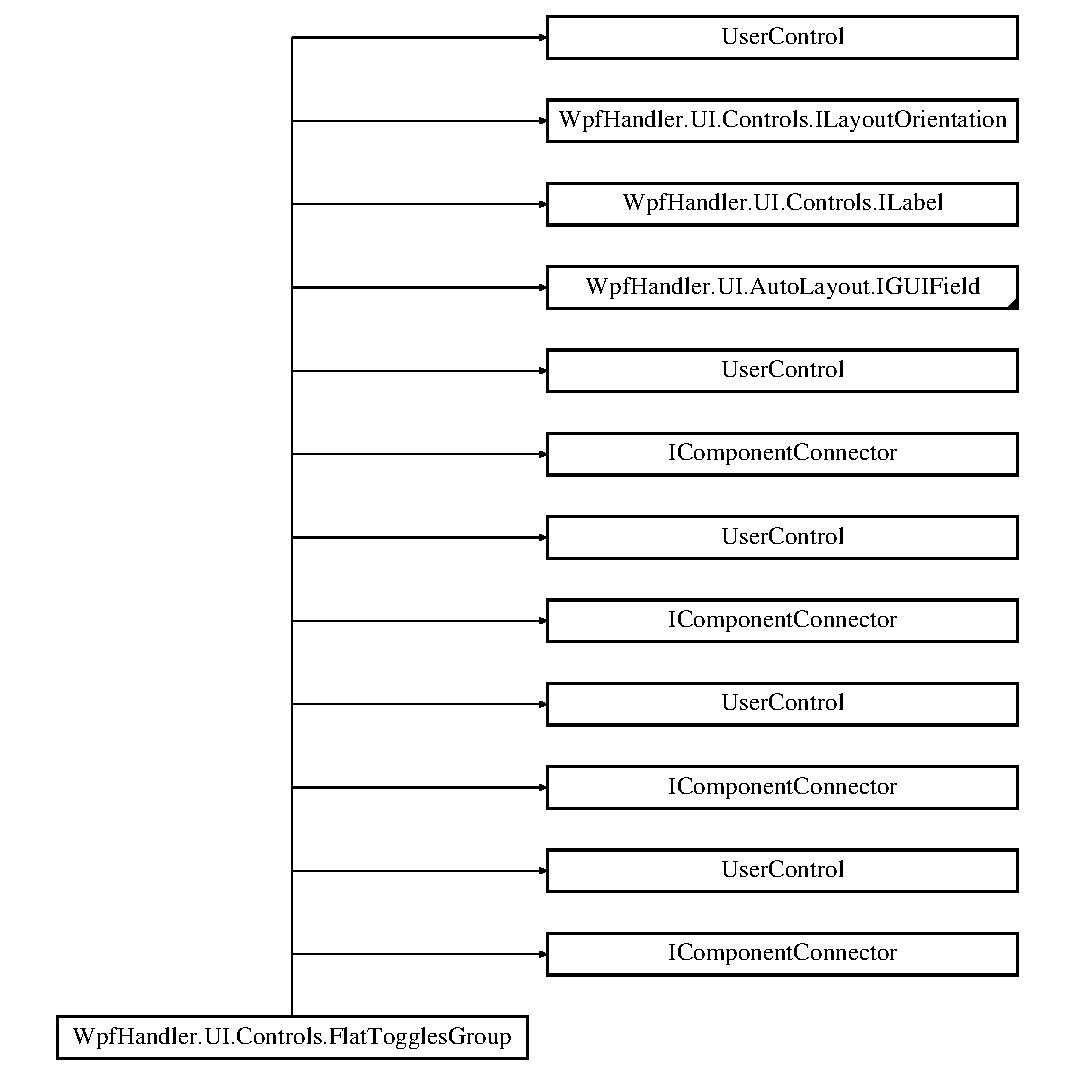
\includegraphics[height=12.000000cm]{dd/dae/class_wpf_handler_1_1_u_i_1_1_controls_1_1_flat_toggles_group}
\end{center}
\end{figure}
\subsection*{Public Member Functions}
\begin{DoxyCompactItemize}
\item 
void \mbox{\hyperlink{class_wpf_handler_1_1_u_i_1_1_controls_1_1_flat_toggles_group_a6bf13c1fc4d0e238190ce92895b8123c}{Initialize\+Component}} ()
\begin{DoxyCompactList}\small\item\em Initialize\+Component \end{DoxyCompactList}\item 
void \mbox{\hyperlink{class_wpf_handler_1_1_u_i_1_1_controls_1_1_flat_toggles_group_a6bf13c1fc4d0e238190ce92895b8123c}{Initialize\+Component}} ()
\begin{DoxyCompactList}\small\item\em Initialize\+Component \end{DoxyCompactList}\item 
void \mbox{\hyperlink{class_wpf_handler_1_1_u_i_1_1_controls_1_1_flat_toggles_group_a6bf13c1fc4d0e238190ce92895b8123c}{Initialize\+Component}} ()
\begin{DoxyCompactList}\small\item\em Initialize\+Component \end{DoxyCompactList}\item 
void \mbox{\hyperlink{class_wpf_handler_1_1_u_i_1_1_controls_1_1_flat_toggles_group_a6bf13c1fc4d0e238190ce92895b8123c}{Initialize\+Component}} ()
\begin{DoxyCompactList}\small\item\em Initialize\+Component \end{DoxyCompactList}\item 
\mbox{\hyperlink{class_wpf_handler_1_1_u_i_1_1_controls_1_1_flat_toggles_group_a026f873b2f214e35ee3f3ad5715e1bad}{Flat\+Toggles\+Group}} ()
\begin{DoxyCompactList}\small\item\em Initialize component. \end{DoxyCompactList}\item 
void \mbox{\hyperlink{class_wpf_handler_1_1_u_i_1_1_controls_1_1_flat_toggles_group_a5619e5107d6cbc3fb2cdabb21deb40a4}{On\+Layout}} (ref \mbox{\hyperlink{class_wpf_handler_1_1_u_i_1_1_auto_layout_1_1_layout_layer}{Layout\+Layer}} layer, params object\mbox{[}$\,$\mbox{]} args)
\begin{DoxyCompactList}\small\item\em Modify current layer\textquotesingle{}s layout according to G\+UI element requirments. Calls once during \mbox{\hyperlink{namespace_wpf_handler_1_1_u_i}{UI}} spawn. \end{DoxyCompactList}\item 
void \mbox{\hyperlink{class_wpf_handler_1_1_u_i_1_1_controls_1_1_flat_toggles_group_a614b0a059caad9bc0704342bae1bb7f5}{Update\+Elements\+Layout}} ()
\begin{DoxyCompactList}\small\item\em Applying relevant layout to the elements. \end{DoxyCompactList}\end{DoxyCompactItemize}
\subsection*{Static Public Attributes}
\begin{DoxyCompactItemize}
\item 
static readonly Dependency\+Property \mbox{\hyperlink{class_wpf_handler_1_1_u_i_1_1_controls_1_1_flat_toggles_group_a72591a66a8b72130cf16e966bbed5507}{Label\+Property}}
\begin{DoxyCompactList}\small\item\em Property that bridging control\textquotesingle{}s property between X\+A\+ML and code. \end{DoxyCompactList}\item 
static readonly Dependency\+Property \mbox{\hyperlink{class_wpf_handler_1_1_u_i_1_1_controls_1_1_flat_toggles_group_acd4cc98db2da7479ac81dd03ceaadcae}{Label\+Width\+Property}}
\begin{DoxyCompactList}\small\item\em Property that bridging control\textquotesingle{}s property between X\+A\+ML and code. \end{DoxyCompactList}\item 
static readonly Dependency\+Property \mbox{\hyperlink{class_wpf_handler_1_1_u_i_1_1_controls_1_1_flat_toggles_group_a2df8b183c4855b48d46fe14730225db4}{Fields\+Content\+Property}}
\begin{DoxyCompactList}\small\item\em Property that bridging control\textquotesingle{}s property between X\+A\+ML and code. \end{DoxyCompactList}\end{DoxyCompactItemize}
\subsection*{Protected Member Functions}
\begin{DoxyCompactItemize}
\item 
void \mbox{\hyperlink{class_wpf_handler_1_1_u_i_1_1_controls_1_1_flat_toggles_group_a58a008dadfd937ce1379ee16602139bd}{Instiniate\+Elements}} ()
\begin{DoxyCompactList}\small\item\em Instiniating \mbox{\hyperlink{namespace_wpf_handler_1_1_u_i}{UI}} elements from binded meta. \end{DoxyCompactList}\item 
void \mbox{\hyperlink{class_wpf_handler_1_1_u_i_1_1_controls_1_1_flat_toggles_group_a02dd935c06724428d0782839f0035189}{Instiniate\+Custom\+Elements}} ()
\begin{DoxyCompactList}\small\item\em Instiniating elelements for the custom \mbox{\hyperlink{class_wpf_handler_1_1_u_i_1_1_controls_1_1_flat_toggles_group_a48c85f0f2ca803d28b95877dbc0122f0}{Fields\+Content}} list. \end{DoxyCompactList}\item 
void \mbox{\hyperlink{class_wpf_handler_1_1_u_i_1_1_controls_1_1_flat_toggles_group_af854af2e1f2768daedecb38eb983072f}{Instiniate\+Enum\+Elements}} ()
\begin{DoxyCompactList}\small\item\em Instiniated elements by the binded Enum type. \end{DoxyCompactList}\item 
void \mbox{\hyperlink{class_wpf_handler_1_1_u_i_1_1_controls_1_1_flat_toggles_group_a8e8bd8928ac0cba35f35554adad3f077}{User\+Control\+\_\+\+Loaded}} (object sender, Routed\+Event\+Args e)
\begin{DoxyCompactList}\small\item\em Occurs when the element is loaded. \end{DoxyCompactList}\end{DoxyCompactItemize}
\subsection*{Protected Attributes}
\begin{DoxyCompactItemize}
\item 
float \mbox{\hyperlink{class_wpf_handler_1_1_u_i_1_1_controls_1_1_flat_toggles_group_ab56d0f33fd489259568de7a64b14487d}{Last\+Label\+Width}} = 0
\begin{DoxyCompactList}\small\item\em Bufer that contains las requested label width. \end{DoxyCompactList}\item 
\mbox{\hyperlink{class_wpf_handler_1_1_u_i_1_1_controls_1_1_flat_toggles_group_ab0cb4350ceae1f1288d6c83de4ed66c9}{Orientation}} \mbox{\hyperlink{class_wpf_handler_1_1_u_i_1_1_controls_1_1_flat_toggles_group_af7f9d34a746082b32a92ae1cb7e338f2}{\+\_\+\+Orientation}} = Orientation.\+Vertical
\begin{DoxyCompactList}\small\item\em Bufer that contains current layout orientation. \end{DoxyCompactList}\item 
int \mbox{\hyperlink{class_wpf_handler_1_1_u_i_1_1_controls_1_1_flat_toggles_group_a559848ddfbcddd8620d9a7783d2a7d04}{\+\_\+\+Index}} = 0
\begin{DoxyCompactList}\small\item\em Bufer that contains selected index. \end{DoxyCompactList}\item 
Member\+Info \mbox{\hyperlink{class_wpf_handler_1_1_u_i_1_1_controls_1_1_flat_toggles_group_a4c0eac437404a019551b6bfd102cc034}{\+\_\+\+Binded\+Member}}
\begin{DoxyCompactList}\small\item\em Bufer that contains reference to the binded member. \end{DoxyCompactList}\item 
Array \mbox{\hyperlink{class_wpf_handler_1_1_u_i_1_1_controls_1_1_flat_toggles_group_afce8c50c94f3417c807a2ba7cce7970f}{\+\_\+\+Values}}
\begin{DoxyCompactList}\small\item\em Bufer that contains the values of the binded enum. \end{DoxyCompactList}\item 
Framework\+Element \mbox{[}$\,$\mbox{]} \mbox{\hyperlink{class_wpf_handler_1_1_u_i_1_1_controls_1_1_flat_toggles_group_ad8b50e4aed5842fb4b3814a281d6cb31}{\+\_\+\+Elements}}
\begin{DoxyCompactList}\small\item\em Array that contains instiniated \mbox{\hyperlink{namespace_wpf_handler_1_1_u_i}{UI}} elements. \end{DoxyCompactList}\end{DoxyCompactItemize}
\subsection*{Package Attributes}
\begin{DoxyCompactItemize}
\item 
\mbox{\Hypertarget{class_wpf_handler_1_1_u_i_1_1_controls_1_1_flat_toggles_group_a20542cd1b273f10a8df98d4b403f0a49}\label{class_wpf_handler_1_1_u_i_1_1_controls_1_1_flat_toggles_group_a20542cd1b273f10a8df98d4b403f0a49}} 
System.\+Windows.\+Controls.\+Grid {\bfseries canvas}
\item 
\mbox{\Hypertarget{class_wpf_handler_1_1_u_i_1_1_controls_1_1_flat_toggles_group_ad45e117a4853bf701b9e5613f861c90d}\label{class_wpf_handler_1_1_u_i_1_1_controls_1_1_flat_toggles_group_ad45e117a4853bf701b9e5613f861c90d}} 
System.\+Windows.\+Controls.\+Label {\bfseries label}
\end{DoxyCompactItemize}
\subsection*{Properties}
\begin{DoxyCompactItemize}
\item 
Type \mbox{\hyperlink{class_wpf_handler_1_1_u_i_1_1_controls_1_1_flat_toggles_group_abb4f90b5eace0651db2af6f293d312d1}{Binded\+Enum\+Type}}\hspace{0.3cm}{\ttfamily  \mbox{[}get, protected set\mbox{]}}
\begin{DoxyCompactList}\small\item\em Type that binded to that G\+UI element. \end{DoxyCompactList}\item 
Array \mbox{\hyperlink{class_wpf_handler_1_1_u_i_1_1_controls_1_1_flat_toggles_group_a146fc04548cdc1df39cd8c9c1d4b3b00}{Values}}\hspace{0.3cm}{\ttfamily  \mbox{[}get\mbox{]}}
\begin{DoxyCompactList}\small\item\em Return an array with values of the binded tnum type. Using the \mbox{\hyperlink{class_wpf_handler_1_1_u_i_1_1_controls_1_1_flat_toggles_group_a48c85f0f2ca803d28b95877dbc0122f0}{Fields\+Content}} in case if \mbox{\hyperlink{class_wpf_handler_1_1_u_i_1_1_controls_1_1_flat_toggles_group_abb4f90b5eace0651db2af6f293d312d1}{Binded\+Enum\+Type}} is null. \end{DoxyCompactList}\item 
Orientation \mbox{\hyperlink{class_wpf_handler_1_1_u_i_1_1_controls_1_1_flat_toggles_group_ab0cb4350ceae1f1288d6c83de4ed66c9}{Orientation}}\hspace{0.3cm}{\ttfamily  \mbox{[}get, set\mbox{]}}
\begin{DoxyCompactList}\small\item\em Layout orientation of the \mbox{\hyperlink{namespace_wpf_handler_1_1_u_i}{UI}} elements. \end{DoxyCompactList}\item 
Framework\+Element \mbox{[}$\,$\mbox{]} \mbox{\hyperlink{class_wpf_handler_1_1_u_i_1_1_controls_1_1_flat_toggles_group_af11956552285c0b69219ab52362d3646}{Elements}}\hspace{0.3cm}{\ttfamily  \mbox{[}get, protected set\mbox{]}}
\begin{DoxyCompactList}\small\item\em Instiniated element in direct order. \end{DoxyCompactList}\item 
Array \mbox{\hyperlink{class_wpf_handler_1_1_u_i_1_1_controls_1_1_flat_toggles_group_a48c85f0f2ca803d28b95877dbc0122f0}{Fields\+Content}}\hspace{0.3cm}{\ttfamily  \mbox{[}get, set\mbox{]}}
\begin{DoxyCompactList}\small\item\em Text in label field. \end{DoxyCompactList}\item 
string \mbox{\hyperlink{class_wpf_handler_1_1_u_i_1_1_controls_1_1_flat_toggles_group_a49e224a3505a7214029943dd421e4cd6}{Label}}\hspace{0.3cm}{\ttfamily  \mbox{[}get, set\mbox{]}}
\begin{DoxyCompactList}\small\item\em Text in label field. \end{DoxyCompactList}\item 
float \mbox{\hyperlink{class_wpf_handler_1_1_u_i_1_1_controls_1_1_flat_toggles_group_a183897b270682950d9a7fa6cc8bd7e0f}{Label\+Width}}\hspace{0.3cm}{\ttfamily  \mbox{[}get, set\mbox{]}}
\begin{DoxyCompactList}\small\item\em Width of label field. \end{DoxyCompactList}\item 
object \mbox{\hyperlink{class_wpf_handler_1_1_u_i_1_1_controls_1_1_flat_toggles_group_a699f90c459005d9501720e719859ba96}{Value}}\hspace{0.3cm}{\ttfamily  \mbox{[}get, set\mbox{]}}
\begin{DoxyCompactList}\small\item\em Value of that control. \end{DoxyCompactList}\item 
int \mbox{\hyperlink{class_wpf_handler_1_1_u_i_1_1_controls_1_1_flat_toggles_group_a89cc073c7cd5761d1700f8d545ae72df}{Index}}\hspace{0.3cm}{\ttfamily  \mbox{[}get, set\mbox{]}}
\begin{DoxyCompactList}\small\item\em Current selected element in the group. \end{DoxyCompactList}\item 
Framework\+Element \mbox{\hyperlink{class_wpf_handler_1_1_u_i_1_1_controls_1_1_flat_toggles_group_a32cdb6b0e4be63ed1465645f6ea7b16b}{Selected\+Element}}\hspace{0.3cm}{\ttfamily  \mbox{[}get\mbox{]}}
\begin{DoxyCompactList}\small\item\em Returns current selected \mbox{\hyperlink{namespace_wpf_handler_1_1_u_i}{UI}} element. \end{DoxyCompactList}\item 
Member\+Info \mbox{\hyperlink{class_wpf_handler_1_1_u_i_1_1_controls_1_1_flat_toggles_group_a23b02958e22396a5fb45255cad69eac0}{Binded\+Member}}\hspace{0.3cm}{\ttfamily  \mbox{[}get, set\mbox{]}}
\begin{DoxyCompactList}\small\item\em Memeber that will be used as source for the value into \mbox{\hyperlink{namespace_wpf_handler_1_1_u_i}{UI}}. \end{DoxyCompactList}\item 
Panel \mbox{\hyperlink{class_wpf_handler_1_1_u_i_1_1_controls_1_1_flat_toggles_group_a89515b615bad1290bf2342ff791b8f16}{Items\+Panel}}\hspace{0.3cm}{\ttfamily  \mbox{[}get, protected set\mbox{]}}
\begin{DoxyCompactList}\small\item\em Panel that contains instiniated elemtnts. \end{DoxyCompactList}\end{DoxyCompactItemize}
\subsection*{Events}
\begin{DoxyCompactItemize}
\item 
Action$<$ \mbox{\hyperlink{interface_wpf_handler_1_1_u_i_1_1_auto_layout_1_1_i_g_u_i_field}{I\+G\+U\+I\+Field}} $>$ \mbox{\hyperlink{class_wpf_handler_1_1_u_i_1_1_controls_1_1_flat_toggles_group_aa00366c7443bee714b067ee15186de82}{Value\+Changed}}
\begin{DoxyCompactList}\small\item\em Event that will occure in case if value of the field will be changed. Will cause updating of the Binded\+Member value. \end{DoxyCompactList}\end{DoxyCompactItemize}
\subsection*{Private Member Functions}
\begin{DoxyCompactItemize}
\item 
\mbox{\Hypertarget{class_wpf_handler_1_1_u_i_1_1_controls_1_1_flat_toggles_group_ac714bc342f0c8121d2adb1585696110c}\label{class_wpf_handler_1_1_u_i_1_1_controls_1_1_flat_toggles_group_ac714bc342f0c8121d2adb1585696110c}} 
void System.\+Windows.\+Markup.\+I\+Component\+Connector. {\bfseries Connect} (int connection\+Id, object target)
\item 
\mbox{\Hypertarget{class_wpf_handler_1_1_u_i_1_1_controls_1_1_flat_toggles_group_ac714bc342f0c8121d2adb1585696110c}\label{class_wpf_handler_1_1_u_i_1_1_controls_1_1_flat_toggles_group_ac714bc342f0c8121d2adb1585696110c}} 
void System.\+Windows.\+Markup.\+I\+Component\+Connector. {\bfseries Connect} (int connection\+Id, object target)
\item 
\mbox{\Hypertarget{class_wpf_handler_1_1_u_i_1_1_controls_1_1_flat_toggles_group_ac714bc342f0c8121d2adb1585696110c}\label{class_wpf_handler_1_1_u_i_1_1_controls_1_1_flat_toggles_group_ac714bc342f0c8121d2adb1585696110c}} 
void System.\+Windows.\+Markup.\+I\+Component\+Connector. {\bfseries Connect} (int connection\+Id, object target)
\item 
\mbox{\Hypertarget{class_wpf_handler_1_1_u_i_1_1_controls_1_1_flat_toggles_group_ac714bc342f0c8121d2adb1585696110c}\label{class_wpf_handler_1_1_u_i_1_1_controls_1_1_flat_toggles_group_ac714bc342f0c8121d2adb1585696110c}} 
void System.\+Windows.\+Markup.\+I\+Component\+Connector. {\bfseries Connect} (int connection\+Id, object target)
\end{DoxyCompactItemize}
\subsection*{Private Attributes}
\begin{DoxyCompactItemize}
\item 
\mbox{\Hypertarget{class_wpf_handler_1_1_u_i_1_1_controls_1_1_flat_toggles_group_a07a25f02db300f347d12a32175acc88b}\label{class_wpf_handler_1_1_u_i_1_1_controls_1_1_flat_toggles_group_a07a25f02db300f347d12a32175acc88b}} 
bool {\bfseries \+\_\+content\+Loaded}
\end{DoxyCompactItemize}


\subsection{Detailed Description}
\mbox{\hyperlink{class_wpf_handler_1_1_u_i_1_1_controls_1_1_flat_toggles_group}{Flat\+Toggles\+Group}} 

T\+O\+DO\+: Operating by group of the toggles. 

\subsection{Constructor \& Destructor Documentation}
\mbox{\Hypertarget{class_wpf_handler_1_1_u_i_1_1_controls_1_1_flat_toggles_group_a026f873b2f214e35ee3f3ad5715e1bad}\label{class_wpf_handler_1_1_u_i_1_1_controls_1_1_flat_toggles_group_a026f873b2f214e35ee3f3ad5715e1bad}} 
\index{Wpf\+Handler\+::\+U\+I\+::\+Controls\+::\+Flat\+Toggles\+Group@{Wpf\+Handler\+::\+U\+I\+::\+Controls\+::\+Flat\+Toggles\+Group}!Flat\+Toggles\+Group@{Flat\+Toggles\+Group}}
\index{Flat\+Toggles\+Group@{Flat\+Toggles\+Group}!Wpf\+Handler\+::\+U\+I\+::\+Controls\+::\+Flat\+Toggles\+Group@{Wpf\+Handler\+::\+U\+I\+::\+Controls\+::\+Flat\+Toggles\+Group}}
\subsubsection{\texorpdfstring{Flat\+Toggles\+Group()}{FlatTogglesGroup()}}
{\footnotesize\ttfamily Wpf\+Handler.\+U\+I.\+Controls.\+Flat\+Toggles\+Group.\+Flat\+Toggles\+Group (\begin{DoxyParamCaption}{ }\end{DoxyParamCaption})}



Initialize component. 



\subsection{Member Function Documentation}
\mbox{\Hypertarget{class_wpf_handler_1_1_u_i_1_1_controls_1_1_flat_toggles_group_a6bf13c1fc4d0e238190ce92895b8123c}\label{class_wpf_handler_1_1_u_i_1_1_controls_1_1_flat_toggles_group_a6bf13c1fc4d0e238190ce92895b8123c}} 
\index{Wpf\+Handler\+::\+U\+I\+::\+Controls\+::\+Flat\+Toggles\+Group@{Wpf\+Handler\+::\+U\+I\+::\+Controls\+::\+Flat\+Toggles\+Group}!Initialize\+Component@{Initialize\+Component}}
\index{Initialize\+Component@{Initialize\+Component}!Wpf\+Handler\+::\+U\+I\+::\+Controls\+::\+Flat\+Toggles\+Group@{Wpf\+Handler\+::\+U\+I\+::\+Controls\+::\+Flat\+Toggles\+Group}}
\subsubsection{\texorpdfstring{Initialize\+Component()}{InitializeComponent()}\hspace{0.1cm}{\footnotesize\ttfamily [1/4]}}
{\footnotesize\ttfamily void Wpf\+Handler.\+U\+I.\+Controls.\+Flat\+Toggles\+Group.\+Initialize\+Component (\begin{DoxyParamCaption}{ }\end{DoxyParamCaption})}



Initialize\+Component 

\mbox{\Hypertarget{class_wpf_handler_1_1_u_i_1_1_controls_1_1_flat_toggles_group_a6bf13c1fc4d0e238190ce92895b8123c}\label{class_wpf_handler_1_1_u_i_1_1_controls_1_1_flat_toggles_group_a6bf13c1fc4d0e238190ce92895b8123c}} 
\index{Wpf\+Handler\+::\+U\+I\+::\+Controls\+::\+Flat\+Toggles\+Group@{Wpf\+Handler\+::\+U\+I\+::\+Controls\+::\+Flat\+Toggles\+Group}!Initialize\+Component@{Initialize\+Component}}
\index{Initialize\+Component@{Initialize\+Component}!Wpf\+Handler\+::\+U\+I\+::\+Controls\+::\+Flat\+Toggles\+Group@{Wpf\+Handler\+::\+U\+I\+::\+Controls\+::\+Flat\+Toggles\+Group}}
\subsubsection{\texorpdfstring{Initialize\+Component()}{InitializeComponent()}\hspace{0.1cm}{\footnotesize\ttfamily [2/4]}}
{\footnotesize\ttfamily void Wpf\+Handler.\+U\+I.\+Controls.\+Flat\+Toggles\+Group.\+Initialize\+Component (\begin{DoxyParamCaption}{ }\end{DoxyParamCaption})}



Initialize\+Component 

\mbox{\Hypertarget{class_wpf_handler_1_1_u_i_1_1_controls_1_1_flat_toggles_group_a6bf13c1fc4d0e238190ce92895b8123c}\label{class_wpf_handler_1_1_u_i_1_1_controls_1_1_flat_toggles_group_a6bf13c1fc4d0e238190ce92895b8123c}} 
\index{Wpf\+Handler\+::\+U\+I\+::\+Controls\+::\+Flat\+Toggles\+Group@{Wpf\+Handler\+::\+U\+I\+::\+Controls\+::\+Flat\+Toggles\+Group}!Initialize\+Component@{Initialize\+Component}}
\index{Initialize\+Component@{Initialize\+Component}!Wpf\+Handler\+::\+U\+I\+::\+Controls\+::\+Flat\+Toggles\+Group@{Wpf\+Handler\+::\+U\+I\+::\+Controls\+::\+Flat\+Toggles\+Group}}
\subsubsection{\texorpdfstring{Initialize\+Component()}{InitializeComponent()}\hspace{0.1cm}{\footnotesize\ttfamily [3/4]}}
{\footnotesize\ttfamily void Wpf\+Handler.\+U\+I.\+Controls.\+Flat\+Toggles\+Group.\+Initialize\+Component (\begin{DoxyParamCaption}{ }\end{DoxyParamCaption})}



Initialize\+Component 

\mbox{\Hypertarget{class_wpf_handler_1_1_u_i_1_1_controls_1_1_flat_toggles_group_a6bf13c1fc4d0e238190ce92895b8123c}\label{class_wpf_handler_1_1_u_i_1_1_controls_1_1_flat_toggles_group_a6bf13c1fc4d0e238190ce92895b8123c}} 
\index{Wpf\+Handler\+::\+U\+I\+::\+Controls\+::\+Flat\+Toggles\+Group@{Wpf\+Handler\+::\+U\+I\+::\+Controls\+::\+Flat\+Toggles\+Group}!Initialize\+Component@{Initialize\+Component}}
\index{Initialize\+Component@{Initialize\+Component}!Wpf\+Handler\+::\+U\+I\+::\+Controls\+::\+Flat\+Toggles\+Group@{Wpf\+Handler\+::\+U\+I\+::\+Controls\+::\+Flat\+Toggles\+Group}}
\subsubsection{\texorpdfstring{Initialize\+Component()}{InitializeComponent()}\hspace{0.1cm}{\footnotesize\ttfamily [4/4]}}
{\footnotesize\ttfamily void Wpf\+Handler.\+U\+I.\+Controls.\+Flat\+Toggles\+Group.\+Initialize\+Component (\begin{DoxyParamCaption}{ }\end{DoxyParamCaption})}



Initialize\+Component 

\mbox{\Hypertarget{class_wpf_handler_1_1_u_i_1_1_controls_1_1_flat_toggles_group_a02dd935c06724428d0782839f0035189}\label{class_wpf_handler_1_1_u_i_1_1_controls_1_1_flat_toggles_group_a02dd935c06724428d0782839f0035189}} 
\index{Wpf\+Handler\+::\+U\+I\+::\+Controls\+::\+Flat\+Toggles\+Group@{Wpf\+Handler\+::\+U\+I\+::\+Controls\+::\+Flat\+Toggles\+Group}!Instiniate\+Custom\+Elements@{Instiniate\+Custom\+Elements}}
\index{Instiniate\+Custom\+Elements@{Instiniate\+Custom\+Elements}!Wpf\+Handler\+::\+U\+I\+::\+Controls\+::\+Flat\+Toggles\+Group@{Wpf\+Handler\+::\+U\+I\+::\+Controls\+::\+Flat\+Toggles\+Group}}
\subsubsection{\texorpdfstring{Instiniate\+Custom\+Elements()}{InstiniateCustomElements()}}
{\footnotesize\ttfamily void Wpf\+Handler.\+U\+I.\+Controls.\+Flat\+Toggles\+Group.\+Instiniate\+Custom\+Elements (\begin{DoxyParamCaption}{ }\end{DoxyParamCaption})\hspace{0.3cm}{\ttfamily [protected]}}



Instiniating elelements for the custom \mbox{\hyperlink{class_wpf_handler_1_1_u_i_1_1_controls_1_1_flat_toggles_group_a48c85f0f2ca803d28b95877dbc0122f0}{Fields\+Content}} list. 

\mbox{\Hypertarget{class_wpf_handler_1_1_u_i_1_1_controls_1_1_flat_toggles_group_a58a008dadfd937ce1379ee16602139bd}\label{class_wpf_handler_1_1_u_i_1_1_controls_1_1_flat_toggles_group_a58a008dadfd937ce1379ee16602139bd}} 
\index{Wpf\+Handler\+::\+U\+I\+::\+Controls\+::\+Flat\+Toggles\+Group@{Wpf\+Handler\+::\+U\+I\+::\+Controls\+::\+Flat\+Toggles\+Group}!Instiniate\+Elements@{Instiniate\+Elements}}
\index{Instiniate\+Elements@{Instiniate\+Elements}!Wpf\+Handler\+::\+U\+I\+::\+Controls\+::\+Flat\+Toggles\+Group@{Wpf\+Handler\+::\+U\+I\+::\+Controls\+::\+Flat\+Toggles\+Group}}
\subsubsection{\texorpdfstring{Instiniate\+Elements()}{InstiniateElements()}}
{\footnotesize\ttfamily void Wpf\+Handler.\+U\+I.\+Controls.\+Flat\+Toggles\+Group.\+Instiniate\+Elements (\begin{DoxyParamCaption}{ }\end{DoxyParamCaption})\hspace{0.3cm}{\ttfamily [protected]}}



Instiniating \mbox{\hyperlink{namespace_wpf_handler_1_1_u_i}{UI}} elements from binded meta. 

\mbox{\Hypertarget{class_wpf_handler_1_1_u_i_1_1_controls_1_1_flat_toggles_group_af854af2e1f2768daedecb38eb983072f}\label{class_wpf_handler_1_1_u_i_1_1_controls_1_1_flat_toggles_group_af854af2e1f2768daedecb38eb983072f}} 
\index{Wpf\+Handler\+::\+U\+I\+::\+Controls\+::\+Flat\+Toggles\+Group@{Wpf\+Handler\+::\+U\+I\+::\+Controls\+::\+Flat\+Toggles\+Group}!Instiniate\+Enum\+Elements@{Instiniate\+Enum\+Elements}}
\index{Instiniate\+Enum\+Elements@{Instiniate\+Enum\+Elements}!Wpf\+Handler\+::\+U\+I\+::\+Controls\+::\+Flat\+Toggles\+Group@{Wpf\+Handler\+::\+U\+I\+::\+Controls\+::\+Flat\+Toggles\+Group}}
\subsubsection{\texorpdfstring{Instiniate\+Enum\+Elements()}{InstiniateEnumElements()}}
{\footnotesize\ttfamily void Wpf\+Handler.\+U\+I.\+Controls.\+Flat\+Toggles\+Group.\+Instiniate\+Enum\+Elements (\begin{DoxyParamCaption}{ }\end{DoxyParamCaption})\hspace{0.3cm}{\ttfamily [protected]}}



Instiniated elements by the binded Enum type. 

\mbox{\Hypertarget{class_wpf_handler_1_1_u_i_1_1_controls_1_1_flat_toggles_group_a5619e5107d6cbc3fb2cdabb21deb40a4}\label{class_wpf_handler_1_1_u_i_1_1_controls_1_1_flat_toggles_group_a5619e5107d6cbc3fb2cdabb21deb40a4}} 
\index{Wpf\+Handler\+::\+U\+I\+::\+Controls\+::\+Flat\+Toggles\+Group@{Wpf\+Handler\+::\+U\+I\+::\+Controls\+::\+Flat\+Toggles\+Group}!On\+Layout@{On\+Layout}}
\index{On\+Layout@{On\+Layout}!Wpf\+Handler\+::\+U\+I\+::\+Controls\+::\+Flat\+Toggles\+Group@{Wpf\+Handler\+::\+U\+I\+::\+Controls\+::\+Flat\+Toggles\+Group}}
\subsubsection{\texorpdfstring{On\+Layout()}{OnLayout()}}
{\footnotesize\ttfamily void Wpf\+Handler.\+U\+I.\+Controls.\+Flat\+Toggles\+Group.\+On\+Layout (\begin{DoxyParamCaption}\item[{ref \mbox{\hyperlink{class_wpf_handler_1_1_u_i_1_1_auto_layout_1_1_layout_layer}{Layout\+Layer}}}]{layer,  }\item[{params object \mbox{[}$\,$\mbox{]}}]{args }\end{DoxyParamCaption})}



Modify current layer\textquotesingle{}s layout according to G\+UI element requirments. Calls once during \mbox{\hyperlink{namespace_wpf_handler_1_1_u_i}{UI}} spawn. 


\begin{DoxyParams}{Parameters}
{\em layer} & Target G\+UI layer.\\
\hline
{\em args} & Shared arguments. Must contains Member\+Info.\\
\hline
\end{DoxyParams}


Allow castomization enum\textquotesingle{}s element by adding multiply Content\+Attribute. First attribute will applied to the common label. Any next Content\+Attribute will be related to the elements by the direct order. 

Implements \mbox{\hyperlink{interface_wpf_handler_1_1_u_i_1_1_auto_layout_1_1_i_g_u_i_element_a0ff16956f8e8187d51e1b36b6b9f894e}{Wpf\+Handler.\+U\+I.\+Auto\+Layout.\+I\+G\+U\+I\+Element}}.

\mbox{\Hypertarget{class_wpf_handler_1_1_u_i_1_1_controls_1_1_flat_toggles_group_a614b0a059caad9bc0704342bae1bb7f5}\label{class_wpf_handler_1_1_u_i_1_1_controls_1_1_flat_toggles_group_a614b0a059caad9bc0704342bae1bb7f5}} 
\index{Wpf\+Handler\+::\+U\+I\+::\+Controls\+::\+Flat\+Toggles\+Group@{Wpf\+Handler\+::\+U\+I\+::\+Controls\+::\+Flat\+Toggles\+Group}!Update\+Elements\+Layout@{Update\+Elements\+Layout}}
\index{Update\+Elements\+Layout@{Update\+Elements\+Layout}!Wpf\+Handler\+::\+U\+I\+::\+Controls\+::\+Flat\+Toggles\+Group@{Wpf\+Handler\+::\+U\+I\+::\+Controls\+::\+Flat\+Toggles\+Group}}
\subsubsection{\texorpdfstring{Update\+Elements\+Layout()}{UpdateElementsLayout()}}
{\footnotesize\ttfamily void Wpf\+Handler.\+U\+I.\+Controls.\+Flat\+Toggles\+Group.\+Update\+Elements\+Layout (\begin{DoxyParamCaption}{ }\end{DoxyParamCaption})}



Applying relevant layout to the elements. 

\mbox{\Hypertarget{class_wpf_handler_1_1_u_i_1_1_controls_1_1_flat_toggles_group_a8e8bd8928ac0cba35f35554adad3f077}\label{class_wpf_handler_1_1_u_i_1_1_controls_1_1_flat_toggles_group_a8e8bd8928ac0cba35f35554adad3f077}} 
\index{Wpf\+Handler\+::\+U\+I\+::\+Controls\+::\+Flat\+Toggles\+Group@{Wpf\+Handler\+::\+U\+I\+::\+Controls\+::\+Flat\+Toggles\+Group}!User\+Control\+\_\+\+Loaded@{User\+Control\+\_\+\+Loaded}}
\index{User\+Control\+\_\+\+Loaded@{User\+Control\+\_\+\+Loaded}!Wpf\+Handler\+::\+U\+I\+::\+Controls\+::\+Flat\+Toggles\+Group@{Wpf\+Handler\+::\+U\+I\+::\+Controls\+::\+Flat\+Toggles\+Group}}
\subsubsection{\texorpdfstring{User\+Control\+\_\+\+Loaded()}{UserControl\_Loaded()}}
{\footnotesize\ttfamily void Wpf\+Handler.\+U\+I.\+Controls.\+Flat\+Toggles\+Group.\+User\+Control\+\_\+\+Loaded (\begin{DoxyParamCaption}\item[{object}]{sender,  }\item[{Routed\+Event\+Args}]{e }\end{DoxyParamCaption})\hspace{0.3cm}{\ttfamily [protected]}}



Occurs when the element is loaded. 


\begin{DoxyParams}{Parameters}
{\em sender} & \\
\hline
{\em e} & \\
\hline
\end{DoxyParams}


\subsection{Member Data Documentation}
\mbox{\Hypertarget{class_wpf_handler_1_1_u_i_1_1_controls_1_1_flat_toggles_group_a4c0eac437404a019551b6bfd102cc034}\label{class_wpf_handler_1_1_u_i_1_1_controls_1_1_flat_toggles_group_a4c0eac437404a019551b6bfd102cc034}} 
\index{Wpf\+Handler\+::\+U\+I\+::\+Controls\+::\+Flat\+Toggles\+Group@{Wpf\+Handler\+::\+U\+I\+::\+Controls\+::\+Flat\+Toggles\+Group}!\+\_\+\+Binded\+Member@{\+\_\+\+Binded\+Member}}
\index{\+\_\+\+Binded\+Member@{\+\_\+\+Binded\+Member}!Wpf\+Handler\+::\+U\+I\+::\+Controls\+::\+Flat\+Toggles\+Group@{Wpf\+Handler\+::\+U\+I\+::\+Controls\+::\+Flat\+Toggles\+Group}}
\subsubsection{\texorpdfstring{\+\_\+\+Binded\+Member}{\_BindedMember}}
{\footnotesize\ttfamily Member\+Info Wpf\+Handler.\+U\+I.\+Controls.\+Flat\+Toggles\+Group.\+\_\+\+Binded\+Member\hspace{0.3cm}{\ttfamily [protected]}}



Bufer that contains reference to the binded member. 

\mbox{\Hypertarget{class_wpf_handler_1_1_u_i_1_1_controls_1_1_flat_toggles_group_ad8b50e4aed5842fb4b3814a281d6cb31}\label{class_wpf_handler_1_1_u_i_1_1_controls_1_1_flat_toggles_group_ad8b50e4aed5842fb4b3814a281d6cb31}} 
\index{Wpf\+Handler\+::\+U\+I\+::\+Controls\+::\+Flat\+Toggles\+Group@{Wpf\+Handler\+::\+U\+I\+::\+Controls\+::\+Flat\+Toggles\+Group}!\+\_\+\+Elements@{\+\_\+\+Elements}}
\index{\+\_\+\+Elements@{\+\_\+\+Elements}!Wpf\+Handler\+::\+U\+I\+::\+Controls\+::\+Flat\+Toggles\+Group@{Wpf\+Handler\+::\+U\+I\+::\+Controls\+::\+Flat\+Toggles\+Group}}
\subsubsection{\texorpdfstring{\+\_\+\+Elements}{\_Elements}}
{\footnotesize\ttfamily Framework\+Element \mbox{[}$\,$\mbox{]} Wpf\+Handler.\+U\+I.\+Controls.\+Flat\+Toggles\+Group.\+\_\+\+Elements\hspace{0.3cm}{\ttfamily [protected]}}



Array that contains instiniated \mbox{\hyperlink{namespace_wpf_handler_1_1_u_i}{UI}} elements. 

\mbox{\Hypertarget{class_wpf_handler_1_1_u_i_1_1_controls_1_1_flat_toggles_group_a559848ddfbcddd8620d9a7783d2a7d04}\label{class_wpf_handler_1_1_u_i_1_1_controls_1_1_flat_toggles_group_a559848ddfbcddd8620d9a7783d2a7d04}} 
\index{Wpf\+Handler\+::\+U\+I\+::\+Controls\+::\+Flat\+Toggles\+Group@{Wpf\+Handler\+::\+U\+I\+::\+Controls\+::\+Flat\+Toggles\+Group}!\+\_\+\+Index@{\+\_\+\+Index}}
\index{\+\_\+\+Index@{\+\_\+\+Index}!Wpf\+Handler\+::\+U\+I\+::\+Controls\+::\+Flat\+Toggles\+Group@{Wpf\+Handler\+::\+U\+I\+::\+Controls\+::\+Flat\+Toggles\+Group}}
\subsubsection{\texorpdfstring{\+\_\+\+Index}{\_Index}}
{\footnotesize\ttfamily int Wpf\+Handler.\+U\+I.\+Controls.\+Flat\+Toggles\+Group.\+\_\+\+Index = 0\hspace{0.3cm}{\ttfamily [protected]}}



Bufer that contains selected index. 

\mbox{\Hypertarget{class_wpf_handler_1_1_u_i_1_1_controls_1_1_flat_toggles_group_af7f9d34a746082b32a92ae1cb7e338f2}\label{class_wpf_handler_1_1_u_i_1_1_controls_1_1_flat_toggles_group_af7f9d34a746082b32a92ae1cb7e338f2}} 
\index{Wpf\+Handler\+::\+U\+I\+::\+Controls\+::\+Flat\+Toggles\+Group@{Wpf\+Handler\+::\+U\+I\+::\+Controls\+::\+Flat\+Toggles\+Group}!\+\_\+\+Orientation@{\+\_\+\+Orientation}}
\index{\+\_\+\+Orientation@{\+\_\+\+Orientation}!Wpf\+Handler\+::\+U\+I\+::\+Controls\+::\+Flat\+Toggles\+Group@{Wpf\+Handler\+::\+U\+I\+::\+Controls\+::\+Flat\+Toggles\+Group}}
\subsubsection{\texorpdfstring{\+\_\+\+Orientation}{\_Orientation}}
{\footnotesize\ttfamily \mbox{\hyperlink{class_wpf_handler_1_1_u_i_1_1_controls_1_1_flat_toggles_group_ab0cb4350ceae1f1288d6c83de4ed66c9}{Orientation}} Wpf\+Handler.\+U\+I.\+Controls.\+Flat\+Toggles\+Group.\+\_\+\+Orientation = Orientation.\+Vertical\hspace{0.3cm}{\ttfamily [protected]}}



Bufer that contains current layout orientation. 

\mbox{\Hypertarget{class_wpf_handler_1_1_u_i_1_1_controls_1_1_flat_toggles_group_afce8c50c94f3417c807a2ba7cce7970f}\label{class_wpf_handler_1_1_u_i_1_1_controls_1_1_flat_toggles_group_afce8c50c94f3417c807a2ba7cce7970f}} 
\index{Wpf\+Handler\+::\+U\+I\+::\+Controls\+::\+Flat\+Toggles\+Group@{Wpf\+Handler\+::\+U\+I\+::\+Controls\+::\+Flat\+Toggles\+Group}!\+\_\+\+Values@{\+\_\+\+Values}}
\index{\+\_\+\+Values@{\+\_\+\+Values}!Wpf\+Handler\+::\+U\+I\+::\+Controls\+::\+Flat\+Toggles\+Group@{Wpf\+Handler\+::\+U\+I\+::\+Controls\+::\+Flat\+Toggles\+Group}}
\subsubsection{\texorpdfstring{\+\_\+\+Values}{\_Values}}
{\footnotesize\ttfamily Array Wpf\+Handler.\+U\+I.\+Controls.\+Flat\+Toggles\+Group.\+\_\+\+Values\hspace{0.3cm}{\ttfamily [protected]}}



Bufer that contains the values of the binded enum. 

\mbox{\Hypertarget{class_wpf_handler_1_1_u_i_1_1_controls_1_1_flat_toggles_group_a2df8b183c4855b48d46fe14730225db4}\label{class_wpf_handler_1_1_u_i_1_1_controls_1_1_flat_toggles_group_a2df8b183c4855b48d46fe14730225db4}} 
\index{Wpf\+Handler\+::\+U\+I\+::\+Controls\+::\+Flat\+Toggles\+Group@{Wpf\+Handler\+::\+U\+I\+::\+Controls\+::\+Flat\+Toggles\+Group}!Fields\+Content\+Property@{Fields\+Content\+Property}}
\index{Fields\+Content\+Property@{Fields\+Content\+Property}!Wpf\+Handler\+::\+U\+I\+::\+Controls\+::\+Flat\+Toggles\+Group@{Wpf\+Handler\+::\+U\+I\+::\+Controls\+::\+Flat\+Toggles\+Group}}
\subsubsection{\texorpdfstring{Fields\+Content\+Property}{FieldsContentProperty}}
{\footnotesize\ttfamily readonly Dependency\+Property Wpf\+Handler.\+U\+I.\+Controls.\+Flat\+Toggles\+Group.\+Fields\+Content\+Property\hspace{0.3cm}{\ttfamily [static]}}

{\bfseries Initial value\+:}
\begin{DoxyCode}
= DependencyProperty.Register(
          \textcolor{stringliteral}{"FieldsContent"}, typeof(Array), typeof(\mbox{\hyperlink{class_wpf_handler_1_1_u_i_1_1_controls_1_1_flat_toggles_group_a026f873b2f214e35ee3f3ad5715e1bad}{FlatTogglesGroup}}))
\end{DoxyCode}


Property that bridging control\textquotesingle{}s property between X\+A\+ML and code. 

\mbox{\Hypertarget{class_wpf_handler_1_1_u_i_1_1_controls_1_1_flat_toggles_group_a72591a66a8b72130cf16e966bbed5507}\label{class_wpf_handler_1_1_u_i_1_1_controls_1_1_flat_toggles_group_a72591a66a8b72130cf16e966bbed5507}} 
\index{Wpf\+Handler\+::\+U\+I\+::\+Controls\+::\+Flat\+Toggles\+Group@{Wpf\+Handler\+::\+U\+I\+::\+Controls\+::\+Flat\+Toggles\+Group}!Label\+Property@{Label\+Property}}
\index{Label\+Property@{Label\+Property}!Wpf\+Handler\+::\+U\+I\+::\+Controls\+::\+Flat\+Toggles\+Group@{Wpf\+Handler\+::\+U\+I\+::\+Controls\+::\+Flat\+Toggles\+Group}}
\subsubsection{\texorpdfstring{Label\+Property}{LabelProperty}}
{\footnotesize\ttfamily readonly Dependency\+Property Wpf\+Handler.\+U\+I.\+Controls.\+Flat\+Toggles\+Group.\+Label\+Property\hspace{0.3cm}{\ttfamily [static]}}

{\bfseries Initial value\+:}
\begin{DoxyCode}
= DependencyProperty.Register(
          \textcolor{stringliteral}{"Label"}, typeof(\textcolor{keywordtype}{string}), typeof(\mbox{\hyperlink{class_wpf_handler_1_1_u_i_1_1_controls_1_1_flat_toggles_group_a026f873b2f214e35ee3f3ad5715e1bad}{FlatTogglesGroup}}))
\end{DoxyCode}


Property that bridging control\textquotesingle{}s property between X\+A\+ML and code. 

\mbox{\Hypertarget{class_wpf_handler_1_1_u_i_1_1_controls_1_1_flat_toggles_group_acd4cc98db2da7479ac81dd03ceaadcae}\label{class_wpf_handler_1_1_u_i_1_1_controls_1_1_flat_toggles_group_acd4cc98db2da7479ac81dd03ceaadcae}} 
\index{Wpf\+Handler\+::\+U\+I\+::\+Controls\+::\+Flat\+Toggles\+Group@{Wpf\+Handler\+::\+U\+I\+::\+Controls\+::\+Flat\+Toggles\+Group}!Label\+Width\+Property@{Label\+Width\+Property}}
\index{Label\+Width\+Property@{Label\+Width\+Property}!Wpf\+Handler\+::\+U\+I\+::\+Controls\+::\+Flat\+Toggles\+Group@{Wpf\+Handler\+::\+U\+I\+::\+Controls\+::\+Flat\+Toggles\+Group}}
\subsubsection{\texorpdfstring{Label\+Width\+Property}{LabelWidthProperty}}
{\footnotesize\ttfamily readonly Dependency\+Property Wpf\+Handler.\+U\+I.\+Controls.\+Flat\+Toggles\+Group.\+Label\+Width\+Property\hspace{0.3cm}{\ttfamily [static]}}

{\bfseries Initial value\+:}
\begin{DoxyCode}
= DependencyProperty.Register(
          \textcolor{stringliteral}{"LabelWidth"}, typeof(\textcolor{keywordtype}{float}), typeof(\mbox{\hyperlink{class_wpf_handler_1_1_u_i_1_1_controls_1_1_flat_toggles_group_a026f873b2f214e35ee3f3ad5715e1bad}{FlatTogglesGroup}}), \textcolor{keyword}{new} PropertyMetadata(\textcolor{keywordtype}{float}
      .NaN))
\end{DoxyCode}


Property that bridging control\textquotesingle{}s property between X\+A\+ML and code. 

\mbox{\Hypertarget{class_wpf_handler_1_1_u_i_1_1_controls_1_1_flat_toggles_group_ab56d0f33fd489259568de7a64b14487d}\label{class_wpf_handler_1_1_u_i_1_1_controls_1_1_flat_toggles_group_ab56d0f33fd489259568de7a64b14487d}} 
\index{Wpf\+Handler\+::\+U\+I\+::\+Controls\+::\+Flat\+Toggles\+Group@{Wpf\+Handler\+::\+U\+I\+::\+Controls\+::\+Flat\+Toggles\+Group}!Last\+Label\+Width@{Last\+Label\+Width}}
\index{Last\+Label\+Width@{Last\+Label\+Width}!Wpf\+Handler\+::\+U\+I\+::\+Controls\+::\+Flat\+Toggles\+Group@{Wpf\+Handler\+::\+U\+I\+::\+Controls\+::\+Flat\+Toggles\+Group}}
\subsubsection{\texorpdfstring{Last\+Label\+Width}{LastLabelWidth}}
{\footnotesize\ttfamily float Wpf\+Handler.\+U\+I.\+Controls.\+Flat\+Toggles\+Group.\+Last\+Label\+Width = 0\hspace{0.3cm}{\ttfamily [protected]}}



Bufer that contains las requested label width. 



\subsection{Property Documentation}
\mbox{\Hypertarget{class_wpf_handler_1_1_u_i_1_1_controls_1_1_flat_toggles_group_abb4f90b5eace0651db2af6f293d312d1}\label{class_wpf_handler_1_1_u_i_1_1_controls_1_1_flat_toggles_group_abb4f90b5eace0651db2af6f293d312d1}} 
\index{Wpf\+Handler\+::\+U\+I\+::\+Controls\+::\+Flat\+Toggles\+Group@{Wpf\+Handler\+::\+U\+I\+::\+Controls\+::\+Flat\+Toggles\+Group}!Binded\+Enum\+Type@{Binded\+Enum\+Type}}
\index{Binded\+Enum\+Type@{Binded\+Enum\+Type}!Wpf\+Handler\+::\+U\+I\+::\+Controls\+::\+Flat\+Toggles\+Group@{Wpf\+Handler\+::\+U\+I\+::\+Controls\+::\+Flat\+Toggles\+Group}}
\subsubsection{\texorpdfstring{Binded\+Enum\+Type}{BindedEnumType}}
{\footnotesize\ttfamily Type Wpf\+Handler.\+U\+I.\+Controls.\+Flat\+Toggles\+Group.\+Binded\+Enum\+Type\hspace{0.3cm}{\ttfamily [get]}, {\ttfamily [protected set]}}



Type that binded to that G\+UI element. 

\mbox{\Hypertarget{class_wpf_handler_1_1_u_i_1_1_controls_1_1_flat_toggles_group_a23b02958e22396a5fb45255cad69eac0}\label{class_wpf_handler_1_1_u_i_1_1_controls_1_1_flat_toggles_group_a23b02958e22396a5fb45255cad69eac0}} 
\index{Wpf\+Handler\+::\+U\+I\+::\+Controls\+::\+Flat\+Toggles\+Group@{Wpf\+Handler\+::\+U\+I\+::\+Controls\+::\+Flat\+Toggles\+Group}!Binded\+Member@{Binded\+Member}}
\index{Binded\+Member@{Binded\+Member}!Wpf\+Handler\+::\+U\+I\+::\+Controls\+::\+Flat\+Toggles\+Group@{Wpf\+Handler\+::\+U\+I\+::\+Controls\+::\+Flat\+Toggles\+Group}}
\subsubsection{\texorpdfstring{Binded\+Member}{BindedMember}}
{\footnotesize\ttfamily Member\+Info Wpf\+Handler.\+U\+I.\+Controls.\+Flat\+Toggles\+Group.\+Binded\+Member\hspace{0.3cm}{\ttfamily [get]}, {\ttfamily [set]}}



Memeber that will be used as source for the value into \mbox{\hyperlink{namespace_wpf_handler_1_1_u_i}{UI}}. 

The S\+ET option is not supported. \mbox{\Hypertarget{class_wpf_handler_1_1_u_i_1_1_controls_1_1_flat_toggles_group_af11956552285c0b69219ab52362d3646}\label{class_wpf_handler_1_1_u_i_1_1_controls_1_1_flat_toggles_group_af11956552285c0b69219ab52362d3646}} 
\index{Wpf\+Handler\+::\+U\+I\+::\+Controls\+::\+Flat\+Toggles\+Group@{Wpf\+Handler\+::\+U\+I\+::\+Controls\+::\+Flat\+Toggles\+Group}!Elements@{Elements}}
\index{Elements@{Elements}!Wpf\+Handler\+::\+U\+I\+::\+Controls\+::\+Flat\+Toggles\+Group@{Wpf\+Handler\+::\+U\+I\+::\+Controls\+::\+Flat\+Toggles\+Group}}
\subsubsection{\texorpdfstring{Elements}{Elements}}
{\footnotesize\ttfamily Framework\+Element \mbox{[}$\,$\mbox{]} Wpf\+Handler.\+U\+I.\+Controls.\+Flat\+Toggles\+Group.\+Elements\hspace{0.3cm}{\ttfamily [get]}, {\ttfamily [protected set]}}



Instiniated element in direct order. 

\mbox{\Hypertarget{class_wpf_handler_1_1_u_i_1_1_controls_1_1_flat_toggles_group_a48c85f0f2ca803d28b95877dbc0122f0}\label{class_wpf_handler_1_1_u_i_1_1_controls_1_1_flat_toggles_group_a48c85f0f2ca803d28b95877dbc0122f0}} 
\index{Wpf\+Handler\+::\+U\+I\+::\+Controls\+::\+Flat\+Toggles\+Group@{Wpf\+Handler\+::\+U\+I\+::\+Controls\+::\+Flat\+Toggles\+Group}!Fields\+Content@{Fields\+Content}}
\index{Fields\+Content@{Fields\+Content}!Wpf\+Handler\+::\+U\+I\+::\+Controls\+::\+Flat\+Toggles\+Group@{Wpf\+Handler\+::\+U\+I\+::\+Controls\+::\+Flat\+Toggles\+Group}}
\subsubsection{\texorpdfstring{Fields\+Content}{FieldsContent}}
{\footnotesize\ttfamily Array Wpf\+Handler.\+U\+I.\+Controls.\+Flat\+Toggles\+Group.\+Fields\+Content\hspace{0.3cm}{\ttfamily [get]}, {\ttfamily [set]}}



Text in label field. 

\mbox{\Hypertarget{class_wpf_handler_1_1_u_i_1_1_controls_1_1_flat_toggles_group_a89cc073c7cd5761d1700f8d545ae72df}\label{class_wpf_handler_1_1_u_i_1_1_controls_1_1_flat_toggles_group_a89cc073c7cd5761d1700f8d545ae72df}} 
\index{Wpf\+Handler\+::\+U\+I\+::\+Controls\+::\+Flat\+Toggles\+Group@{Wpf\+Handler\+::\+U\+I\+::\+Controls\+::\+Flat\+Toggles\+Group}!Index@{Index}}
\index{Index@{Index}!Wpf\+Handler\+::\+U\+I\+::\+Controls\+::\+Flat\+Toggles\+Group@{Wpf\+Handler\+::\+U\+I\+::\+Controls\+::\+Flat\+Toggles\+Group}}
\subsubsection{\texorpdfstring{Index}{Index}}
{\footnotesize\ttfamily int Wpf\+Handler.\+U\+I.\+Controls.\+Flat\+Toggles\+Group.\+Index\hspace{0.3cm}{\ttfamily [get]}, {\ttfamily [set]}}



Current selected element in the group. 

\mbox{\Hypertarget{class_wpf_handler_1_1_u_i_1_1_controls_1_1_flat_toggles_group_a89515b615bad1290bf2342ff791b8f16}\label{class_wpf_handler_1_1_u_i_1_1_controls_1_1_flat_toggles_group_a89515b615bad1290bf2342ff791b8f16}} 
\index{Wpf\+Handler\+::\+U\+I\+::\+Controls\+::\+Flat\+Toggles\+Group@{Wpf\+Handler\+::\+U\+I\+::\+Controls\+::\+Flat\+Toggles\+Group}!Items\+Panel@{Items\+Panel}}
\index{Items\+Panel@{Items\+Panel}!Wpf\+Handler\+::\+U\+I\+::\+Controls\+::\+Flat\+Toggles\+Group@{Wpf\+Handler\+::\+U\+I\+::\+Controls\+::\+Flat\+Toggles\+Group}}
\subsubsection{\texorpdfstring{Items\+Panel}{ItemsPanel}}
{\footnotesize\ttfamily Panel Wpf\+Handler.\+U\+I.\+Controls.\+Flat\+Toggles\+Group.\+Items\+Panel\hspace{0.3cm}{\ttfamily [get]}, {\ttfamily [protected set]}}



Panel that contains instiniated elemtnts. 

\mbox{\Hypertarget{class_wpf_handler_1_1_u_i_1_1_controls_1_1_flat_toggles_group_a49e224a3505a7214029943dd421e4cd6}\label{class_wpf_handler_1_1_u_i_1_1_controls_1_1_flat_toggles_group_a49e224a3505a7214029943dd421e4cd6}} 
\index{Wpf\+Handler\+::\+U\+I\+::\+Controls\+::\+Flat\+Toggles\+Group@{Wpf\+Handler\+::\+U\+I\+::\+Controls\+::\+Flat\+Toggles\+Group}!Label@{Label}}
\index{Label@{Label}!Wpf\+Handler\+::\+U\+I\+::\+Controls\+::\+Flat\+Toggles\+Group@{Wpf\+Handler\+::\+U\+I\+::\+Controls\+::\+Flat\+Toggles\+Group}}
\subsubsection{\texorpdfstring{Label}{Label}}
{\footnotesize\ttfamily string Wpf\+Handler.\+U\+I.\+Controls.\+Flat\+Toggles\+Group.\+Label\hspace{0.3cm}{\ttfamily [get]}, {\ttfamily [set]}}



Text in label field. 

\mbox{\Hypertarget{class_wpf_handler_1_1_u_i_1_1_controls_1_1_flat_toggles_group_a183897b270682950d9a7fa6cc8bd7e0f}\label{class_wpf_handler_1_1_u_i_1_1_controls_1_1_flat_toggles_group_a183897b270682950d9a7fa6cc8bd7e0f}} 
\index{Wpf\+Handler\+::\+U\+I\+::\+Controls\+::\+Flat\+Toggles\+Group@{Wpf\+Handler\+::\+U\+I\+::\+Controls\+::\+Flat\+Toggles\+Group}!Label\+Width@{Label\+Width}}
\index{Label\+Width@{Label\+Width}!Wpf\+Handler\+::\+U\+I\+::\+Controls\+::\+Flat\+Toggles\+Group@{Wpf\+Handler\+::\+U\+I\+::\+Controls\+::\+Flat\+Toggles\+Group}}
\subsubsection{\texorpdfstring{Label\+Width}{LabelWidth}}
{\footnotesize\ttfamily float Wpf\+Handler.\+U\+I.\+Controls.\+Flat\+Toggles\+Group.\+Label\+Width\hspace{0.3cm}{\ttfamily [get]}, {\ttfamily [set]}}



Width of label field. 

\mbox{\Hypertarget{class_wpf_handler_1_1_u_i_1_1_controls_1_1_flat_toggles_group_ab0cb4350ceae1f1288d6c83de4ed66c9}\label{class_wpf_handler_1_1_u_i_1_1_controls_1_1_flat_toggles_group_ab0cb4350ceae1f1288d6c83de4ed66c9}} 
\index{Wpf\+Handler\+::\+U\+I\+::\+Controls\+::\+Flat\+Toggles\+Group@{Wpf\+Handler\+::\+U\+I\+::\+Controls\+::\+Flat\+Toggles\+Group}!Orientation@{Orientation}}
\index{Orientation@{Orientation}!Wpf\+Handler\+::\+U\+I\+::\+Controls\+::\+Flat\+Toggles\+Group@{Wpf\+Handler\+::\+U\+I\+::\+Controls\+::\+Flat\+Toggles\+Group}}
\subsubsection{\texorpdfstring{Orientation}{Orientation}}
{\footnotesize\ttfamily Orientation Wpf\+Handler.\+U\+I.\+Controls.\+Flat\+Toggles\+Group.\+Orientation\hspace{0.3cm}{\ttfamily [get]}, {\ttfamily [set]}}



Layout orientation of the \mbox{\hyperlink{namespace_wpf_handler_1_1_u_i}{UI}} elements. 

\mbox{\Hypertarget{class_wpf_handler_1_1_u_i_1_1_controls_1_1_flat_toggles_group_a32cdb6b0e4be63ed1465645f6ea7b16b}\label{class_wpf_handler_1_1_u_i_1_1_controls_1_1_flat_toggles_group_a32cdb6b0e4be63ed1465645f6ea7b16b}} 
\index{Wpf\+Handler\+::\+U\+I\+::\+Controls\+::\+Flat\+Toggles\+Group@{Wpf\+Handler\+::\+U\+I\+::\+Controls\+::\+Flat\+Toggles\+Group}!Selected\+Element@{Selected\+Element}}
\index{Selected\+Element@{Selected\+Element}!Wpf\+Handler\+::\+U\+I\+::\+Controls\+::\+Flat\+Toggles\+Group@{Wpf\+Handler\+::\+U\+I\+::\+Controls\+::\+Flat\+Toggles\+Group}}
\subsubsection{\texorpdfstring{Selected\+Element}{SelectedElement}}
{\footnotesize\ttfamily Framework\+Element Wpf\+Handler.\+U\+I.\+Controls.\+Flat\+Toggles\+Group.\+Selected\+Element\hspace{0.3cm}{\ttfamily [get]}}



Returns current selected \mbox{\hyperlink{namespace_wpf_handler_1_1_u_i}{UI}} element. 

\mbox{\Hypertarget{class_wpf_handler_1_1_u_i_1_1_controls_1_1_flat_toggles_group_a699f90c459005d9501720e719859ba96}\label{class_wpf_handler_1_1_u_i_1_1_controls_1_1_flat_toggles_group_a699f90c459005d9501720e719859ba96}} 
\index{Wpf\+Handler\+::\+U\+I\+::\+Controls\+::\+Flat\+Toggles\+Group@{Wpf\+Handler\+::\+U\+I\+::\+Controls\+::\+Flat\+Toggles\+Group}!Value@{Value}}
\index{Value@{Value}!Wpf\+Handler\+::\+U\+I\+::\+Controls\+::\+Flat\+Toggles\+Group@{Wpf\+Handler\+::\+U\+I\+::\+Controls\+::\+Flat\+Toggles\+Group}}
\subsubsection{\texorpdfstring{Value}{Value}}
{\footnotesize\ttfamily object Wpf\+Handler.\+U\+I.\+Controls.\+Flat\+Toggles\+Group.\+Value\hspace{0.3cm}{\ttfamily [get]}, {\ttfamily [set]}}



Value of that control. 

Set allowed only for the enum values. For applying custom list use \mbox{\hyperlink{class_wpf_handler_1_1_u_i_1_1_controls_1_1_flat_toggles_group_a48c85f0f2ca803d28b95877dbc0122f0}{Fields\+Content}} property. \mbox{\Hypertarget{class_wpf_handler_1_1_u_i_1_1_controls_1_1_flat_toggles_group_a146fc04548cdc1df39cd8c9c1d4b3b00}\label{class_wpf_handler_1_1_u_i_1_1_controls_1_1_flat_toggles_group_a146fc04548cdc1df39cd8c9c1d4b3b00}} 
\index{Wpf\+Handler\+::\+U\+I\+::\+Controls\+::\+Flat\+Toggles\+Group@{Wpf\+Handler\+::\+U\+I\+::\+Controls\+::\+Flat\+Toggles\+Group}!Values@{Values}}
\index{Values@{Values}!Wpf\+Handler\+::\+U\+I\+::\+Controls\+::\+Flat\+Toggles\+Group@{Wpf\+Handler\+::\+U\+I\+::\+Controls\+::\+Flat\+Toggles\+Group}}
\subsubsection{\texorpdfstring{Values}{Values}}
{\footnotesize\ttfamily Array Wpf\+Handler.\+U\+I.\+Controls.\+Flat\+Toggles\+Group.\+Values\hspace{0.3cm}{\ttfamily [get]}}



Return an array with values of the binded tnum type. Using the \mbox{\hyperlink{class_wpf_handler_1_1_u_i_1_1_controls_1_1_flat_toggles_group_a48c85f0f2ca803d28b95877dbc0122f0}{Fields\+Content}} in case if \mbox{\hyperlink{class_wpf_handler_1_1_u_i_1_1_controls_1_1_flat_toggles_group_abb4f90b5eace0651db2af6f293d312d1}{Binded\+Enum\+Type}} is null. 



\subsection{Event Documentation}
\mbox{\Hypertarget{class_wpf_handler_1_1_u_i_1_1_controls_1_1_flat_toggles_group_aa00366c7443bee714b067ee15186de82}\label{class_wpf_handler_1_1_u_i_1_1_controls_1_1_flat_toggles_group_aa00366c7443bee714b067ee15186de82}} 
\index{Wpf\+Handler\+::\+U\+I\+::\+Controls\+::\+Flat\+Toggles\+Group@{Wpf\+Handler\+::\+U\+I\+::\+Controls\+::\+Flat\+Toggles\+Group}!Value\+Changed@{Value\+Changed}}
\index{Value\+Changed@{Value\+Changed}!Wpf\+Handler\+::\+U\+I\+::\+Controls\+::\+Flat\+Toggles\+Group@{Wpf\+Handler\+::\+U\+I\+::\+Controls\+::\+Flat\+Toggles\+Group}}
\subsubsection{\texorpdfstring{Value\+Changed}{ValueChanged}}
{\footnotesize\ttfamily Action$<$\mbox{\hyperlink{interface_wpf_handler_1_1_u_i_1_1_auto_layout_1_1_i_g_u_i_field}{I\+G\+U\+I\+Field}}$>$ Wpf\+Handler.\+U\+I.\+Controls.\+Flat\+Toggles\+Group.\+Value\+Changed}



Event that will occure in case if value of the field will be changed. Will cause updating of the Binded\+Member value. 

I\+G\+U\+I\+Field -\/ sender. 

The documentation for this class was generated from the following files\+:\begin{DoxyCompactItemize}
\item 
D\+:/\+Work/\+Git\+Hub/wpf-\/handler/\+Wpf\+Handler/obj/\+Debug/\+U\+I/\+Controls/Flat\+Toggles\+Group.\+g.\+cs\item 
D\+:/\+Work/\+Git\+Hub/wpf-\/handler/\+Wpf\+Handler/obj/\+Debug/\+U\+I/\+Controls/Flat\+Toggles\+Group.\+g.\+i.\+cs\item 
D\+:/\+Work/\+Git\+Hub/wpf-\/handler/\+Wpf\+Handler/\+U\+I/\+Controls/Flat\+Toggles\+Group.\+xaml.\+cs\end{DoxyCompactItemize}

\hypertarget{class_wpf_handler_1_1_u_i_1_1_animations_1_1_float_animation}{}\section{Wpf\+Handler.\+U\+I.\+Animations.\+Float\+Animation Class Reference}
\label{class_wpf_handler_1_1_u_i_1_1_animations_1_1_float_animation}\index{Wpf\+Handler.\+U\+I.\+Animations.\+Float\+Animation@{Wpf\+Handler.\+U\+I.\+Animations.\+Float\+Animation}}


Provide base float animations operations.  


\subsection*{Static Public Member Functions}
\begin{DoxyCompactItemize}
\item 
static Storyboard \mbox{\hyperlink{class_wpf_handler_1_1_u_i_1_1_animations_1_1_float_animation_ac9202e567d294e7f920c55caa8ec6d5d}{Start\+Storyboard}} (Framework\+Element parent, string control\+Name, Property\+Path property\+Path, Time\+Span duration, Fill\+Behavior fill\+Behavior, float from, float to)
\begin{DoxyCompactList}\small\item\em Start float animation. \end{DoxyCompactList}\item 
static Storyboard \mbox{\hyperlink{class_wpf_handler_1_1_u_i_1_1_animations_1_1_float_animation_a54dbe8874dbf79f15995777dfd8993ce}{Start\+Storyboard}} (Framework\+Element parent, string control\+Name, Property\+Path property\+Path, Time\+Span duration, Fill\+Behavior fill\+Behavior, float from, float to, Action$<$ Storyboard $>$ init\+Handler)
\begin{DoxyCompactList}\small\item\em Start float animation. \end{DoxyCompactList}\item 
static Storyboard \mbox{\hyperlink{class_wpf_handler_1_1_u_i_1_1_animations_1_1_float_animation_a6d93b7112e358ffdef4ebb17fb173990}{Start\+Storyboard}} (Framework\+Element parent, Dependency\+Object control, Property\+Path property\+Path, Time\+Span duration, Fill\+Behavior fill\+Behavior, float from, float to, Action$<$ Storyboard $>$ init\+Handler)
\begin{DoxyCompactList}\small\item\em Start float animation. \end{DoxyCompactList}\end{DoxyCompactItemize}


\subsection{Detailed Description}
Provide base float animations operations. 



\subsection{Member Function Documentation}
\mbox{\Hypertarget{class_wpf_handler_1_1_u_i_1_1_animations_1_1_float_animation_ac9202e567d294e7f920c55caa8ec6d5d}\label{class_wpf_handler_1_1_u_i_1_1_animations_1_1_float_animation_ac9202e567d294e7f920c55caa8ec6d5d}} 
\index{Wpf\+Handler\+::\+U\+I\+::\+Animations\+::\+Float\+Animation@{Wpf\+Handler\+::\+U\+I\+::\+Animations\+::\+Float\+Animation}!Start\+Storyboard@{Start\+Storyboard}}
\index{Start\+Storyboard@{Start\+Storyboard}!Wpf\+Handler\+::\+U\+I\+::\+Animations\+::\+Float\+Animation@{Wpf\+Handler\+::\+U\+I\+::\+Animations\+::\+Float\+Animation}}
\subsubsection{\texorpdfstring{Start\+Storyboard()}{StartStoryboard()}\hspace{0.1cm}{\footnotesize\ttfamily [1/3]}}
{\footnotesize\ttfamily static Storyboard Wpf\+Handler.\+U\+I.\+Animations.\+Float\+Animation.\+Start\+Storyboard (\begin{DoxyParamCaption}\item[{Framework\+Element}]{parent,  }\item[{string}]{control\+Name,  }\item[{Property\+Path}]{property\+Path,  }\item[{Time\+Span}]{duration,  }\item[{Fill\+Behavior}]{fill\+Behavior,  }\item[{float}]{from,  }\item[{float}]{to }\end{DoxyParamCaption})\hspace{0.3cm}{\ttfamily [static]}}



Start float animation. 


\begin{DoxyParams}{Parameters}
{\em parent} & Object that contains property.\\
\hline
{\em control\+Name} & A name of the \mbox{\hyperlink{namespace_wpf_handler_1_1_u_i}{UI}} Elemnt.\\
\hline
{\em property\+Path} & A path that describe the dependency property to be animated.\\
\hline
{\em duration} & How many time would take transit.\\
\hline
{\em fill\+Behavior} & Specifies how a System.\+Windows.\+Media.\+Animation.\+Timeline behaves when it is outside its active period but its parent is inside its active or hold period.\\
\hline
{\em from} & Start value.\\
\hline
{\em to} & Finish value.\\
\hline
\end{DoxyParams}
\begin{DoxyReturn}{Returns}
Created storyboard.
\end{DoxyReturn}
\mbox{\Hypertarget{class_wpf_handler_1_1_u_i_1_1_animations_1_1_float_animation_a54dbe8874dbf79f15995777dfd8993ce}\label{class_wpf_handler_1_1_u_i_1_1_animations_1_1_float_animation_a54dbe8874dbf79f15995777dfd8993ce}} 
\index{Wpf\+Handler\+::\+U\+I\+::\+Animations\+::\+Float\+Animation@{Wpf\+Handler\+::\+U\+I\+::\+Animations\+::\+Float\+Animation}!Start\+Storyboard@{Start\+Storyboard}}
\index{Start\+Storyboard@{Start\+Storyboard}!Wpf\+Handler\+::\+U\+I\+::\+Animations\+::\+Float\+Animation@{Wpf\+Handler\+::\+U\+I\+::\+Animations\+::\+Float\+Animation}}
\subsubsection{\texorpdfstring{Start\+Storyboard()}{StartStoryboard()}\hspace{0.1cm}{\footnotesize\ttfamily [2/3]}}
{\footnotesize\ttfamily static Storyboard Wpf\+Handler.\+U\+I.\+Animations.\+Float\+Animation.\+Start\+Storyboard (\begin{DoxyParamCaption}\item[{Framework\+Element}]{parent,  }\item[{string}]{control\+Name,  }\item[{Property\+Path}]{property\+Path,  }\item[{Time\+Span}]{duration,  }\item[{Fill\+Behavior}]{fill\+Behavior,  }\item[{float}]{from,  }\item[{float}]{to,  }\item[{Action$<$ Storyboard $>$}]{init\+Handler }\end{DoxyParamCaption})\hspace{0.3cm}{\ttfamily [static]}}



Start float animation. 


\begin{DoxyParams}{Parameters}
{\em parent} & Object that contains property.\\
\hline
{\em control\+Name} & A name of the \mbox{\hyperlink{namespace_wpf_handler_1_1_u_i}{UI}} element.\\
\hline
{\em property\+Path} & A path that describe the dependency property to be animated.\\
\hline
{\em duration} & How many time would take transit.\\
\hline
{\em fill\+Behavior} & Specifies how a System.\+Windows.\+Media.\+Animation.\+Timeline behaves when it is outside its active period but its parent is inside its active or hold period.\\
\hline
{\em from} & Start value.\\
\hline
{\em to} & Finish value.\\
\hline
{\em init\+Handler} & Handler that would be called before animation start. There you can subscrube on events or reconfigurate settigns.\\
\hline
\end{DoxyParams}
\begin{DoxyReturn}{Returns}
Created storyboard.
\end{DoxyReturn}
\mbox{\Hypertarget{class_wpf_handler_1_1_u_i_1_1_animations_1_1_float_animation_a6d93b7112e358ffdef4ebb17fb173990}\label{class_wpf_handler_1_1_u_i_1_1_animations_1_1_float_animation_a6d93b7112e358ffdef4ebb17fb173990}} 
\index{Wpf\+Handler\+::\+U\+I\+::\+Animations\+::\+Float\+Animation@{Wpf\+Handler\+::\+U\+I\+::\+Animations\+::\+Float\+Animation}!Start\+Storyboard@{Start\+Storyboard}}
\index{Start\+Storyboard@{Start\+Storyboard}!Wpf\+Handler\+::\+U\+I\+::\+Animations\+::\+Float\+Animation@{Wpf\+Handler\+::\+U\+I\+::\+Animations\+::\+Float\+Animation}}
\subsubsection{\texorpdfstring{Start\+Storyboard()}{StartStoryboard()}\hspace{0.1cm}{\footnotesize\ttfamily [3/3]}}
{\footnotesize\ttfamily static Storyboard Wpf\+Handler.\+U\+I.\+Animations.\+Float\+Animation.\+Start\+Storyboard (\begin{DoxyParamCaption}\item[{Framework\+Element}]{parent,  }\item[{Dependency\+Object}]{control,  }\item[{Property\+Path}]{property\+Path,  }\item[{Time\+Span}]{duration,  }\item[{Fill\+Behavior}]{fill\+Behavior,  }\item[{float}]{from,  }\item[{float}]{to,  }\item[{Action$<$ Storyboard $>$}]{init\+Handler }\end{DoxyParamCaption})\hspace{0.3cm}{\ttfamily [static]}}



Start float animation. 


\begin{DoxyParams}{Parameters}
{\em parent} & Object that contains target control.\\
\hline
{\em control} & \mbox{\hyperlink{namespace_wpf_handler_1_1_u_i}{UI}} element that will be animated.\\
\hline
{\em property\+Path} & A path that describe the dependency property to be animated.\\
\hline
{\em duration} & How many time would take transit.\\
\hline
{\em fill\+Behavior} & Specifies how a System.\+Windows.\+Media.\+Animation.\+Timeline behaves when it is outside its active period but its parent is inside its active or hold period.\\
\hline
{\em from} & Start value.\\
\hline
{\em to} & Finish value.\\
\hline
{\em init\+Handler} & Handler that would be called before animation start. There you can subscrube on events or reconfigurate settigns.\\
\hline
\end{DoxyParams}
\begin{DoxyReturn}{Returns}
Created storyboard.
\end{DoxyReturn}


The documentation for this class was generated from the following file\+:\begin{DoxyCompactItemize}
\item 
D\+:/\+Work/\+Git\+Hub/wpf-\/handler/\+Wpf\+Handler/\+U\+I/\+Animations/Float\+Animation.\+cs\end{DoxyCompactItemize}

\hypertarget{class_wpf_handler_1_1_u_i_1_1_auto_layout_1_1_options_1_1_font_size_attribute}{}\section{Wpf\+Handler.\+U\+I.\+Auto\+Layout.\+Options.\+Font\+Size\+Attribute Class Reference}
\label{class_wpf_handler_1_1_u_i_1_1_auto_layout_1_1_options_1_1_font_size_attribute}\index{Wpf\+Handler.\+U\+I.\+Auto\+Layout.\+Options.\+Font\+Size\+Attribute@{Wpf\+Handler.\+U\+I.\+Auto\+Layout.\+Options.\+Font\+Size\+Attribute}}


Define G\+UI element\textquotesingle{}s text font size.  


Inheritance diagram for Wpf\+Handler.\+U\+I.\+Auto\+Layout.\+Options.\+Font\+Size\+Attribute\+:\begin{figure}[H]
\begin{center}
\leavevmode
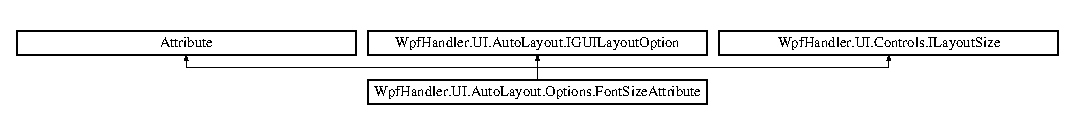
\includegraphics[height=1.177708cm]{d8/d18/class_wpf_handler_1_1_u_i_1_1_auto_layout_1_1_options_1_1_font_size_attribute}
\end{center}
\end{figure}
\subsection*{Public Member Functions}
\begin{DoxyCompactItemize}
\item 
void \mbox{\hyperlink{class_wpf_handler_1_1_u_i_1_1_auto_layout_1_1_options_1_1_font_size_attribute_abd93e70e5419e81c4dfdd9b5d1f35343}{Apply\+Layout\+Option}} (Framework\+Element element)
\begin{DoxyCompactList}\small\item\em Define G\+UI element\textquotesingle{}s text font size. \end{DoxyCompactList}\end{DoxyCompactItemize}
\subsection*{Properties}
\begin{DoxyCompactItemize}
\item 
double \mbox{\hyperlink{class_wpf_handler_1_1_u_i_1_1_auto_layout_1_1_options_1_1_font_size_attribute_a202d0e2cf999904e0a9391cab646bbfc}{Size}} = 14\hspace{0.3cm}{\ttfamily  \mbox{[}get, set\mbox{]}}
\begin{DoxyCompactList}\small\item\em Size of the font in points. \end{DoxyCompactList}\end{DoxyCompactItemize}


\subsection{Detailed Description}
Define G\+UI element\textquotesingle{}s text font size. 



\subsection{Member Function Documentation}
\mbox{\Hypertarget{class_wpf_handler_1_1_u_i_1_1_auto_layout_1_1_options_1_1_font_size_attribute_abd93e70e5419e81c4dfdd9b5d1f35343}\label{class_wpf_handler_1_1_u_i_1_1_auto_layout_1_1_options_1_1_font_size_attribute_abd93e70e5419e81c4dfdd9b5d1f35343}} 
\index{Wpf\+Handler\+::\+U\+I\+::\+Auto\+Layout\+::\+Options\+::\+Font\+Size\+Attribute@{Wpf\+Handler\+::\+U\+I\+::\+Auto\+Layout\+::\+Options\+::\+Font\+Size\+Attribute}!Apply\+Layout\+Option@{Apply\+Layout\+Option}}
\index{Apply\+Layout\+Option@{Apply\+Layout\+Option}!Wpf\+Handler\+::\+U\+I\+::\+Auto\+Layout\+::\+Options\+::\+Font\+Size\+Attribute@{Wpf\+Handler\+::\+U\+I\+::\+Auto\+Layout\+::\+Options\+::\+Font\+Size\+Attribute}}
\subsubsection{\texorpdfstring{Apply\+Layout\+Option()}{ApplyLayoutOption()}}
{\footnotesize\ttfamily void Wpf\+Handler.\+U\+I.\+Auto\+Layout.\+Options.\+Font\+Size\+Attribute.\+Apply\+Layout\+Option (\begin{DoxyParamCaption}\item[{Framework\+Element}]{element }\end{DoxyParamCaption})}



Define G\+UI element\textquotesingle{}s text font size. 


\begin{DoxyParams}{Parameters}
{\em element} & Shared \mbox{\hyperlink{namespace_wpf_handler_1_1_u_i}{UI}} element. Must be inheirted from {\ttfamily System.\+Windows.\+Controls.\+Control} to affect the font properties. \\
\hline
\end{DoxyParams}


Implements \mbox{\hyperlink{interface_wpf_handler_1_1_u_i_1_1_auto_layout_1_1_i_g_u_i_layout_option_ac2d2fa8aeaf753b3248381399f991005}{Wpf\+Handler.\+U\+I.\+Auto\+Layout.\+I\+G\+U\+I\+Layout\+Option}}.



\subsection{Property Documentation}
\mbox{\Hypertarget{class_wpf_handler_1_1_u_i_1_1_auto_layout_1_1_options_1_1_font_size_attribute_a202d0e2cf999904e0a9391cab646bbfc}\label{class_wpf_handler_1_1_u_i_1_1_auto_layout_1_1_options_1_1_font_size_attribute_a202d0e2cf999904e0a9391cab646bbfc}} 
\index{Wpf\+Handler\+::\+U\+I\+::\+Auto\+Layout\+::\+Options\+::\+Font\+Size\+Attribute@{Wpf\+Handler\+::\+U\+I\+::\+Auto\+Layout\+::\+Options\+::\+Font\+Size\+Attribute}!Size@{Size}}
\index{Size@{Size}!Wpf\+Handler\+::\+U\+I\+::\+Auto\+Layout\+::\+Options\+::\+Font\+Size\+Attribute@{Wpf\+Handler\+::\+U\+I\+::\+Auto\+Layout\+::\+Options\+::\+Font\+Size\+Attribute}}
\subsubsection{\texorpdfstring{Size}{Size}}
{\footnotesize\ttfamily double Wpf\+Handler.\+U\+I.\+Auto\+Layout.\+Options.\+Font\+Size\+Attribute.\+Size = 14\hspace{0.3cm}{\ttfamily [get]}, {\ttfamily [set]}}



Size of the font in points. 



The documentation for this class was generated from the following file\+:\begin{DoxyCompactItemize}
\item 
D\+:/\+Work/\+Git\+Hub/wpf-\/handler/\+Wpf\+Handler/\+U\+I/\+Auto\+Layout/\+Options/Font\+Size\+Attribute.\+cs\end{DoxyCompactItemize}

\hypertarget{class_wpf_handler_1_1_u_i_1_1_auto_layout_1_1_options_1_1_foreground_attribute}{}\section{Wpf\+Handler.\+U\+I.\+Auto\+Layout.\+Options.\+Foreground\+Attribute Class Reference}
\label{class_wpf_handler_1_1_u_i_1_1_auto_layout_1_1_options_1_1_foreground_attribute}\index{Wpf\+Handler.\+U\+I.\+Auto\+Layout.\+Options.\+Foreground\+Attribute@{Wpf\+Handler.\+U\+I.\+Auto\+Layout.\+Options.\+Foreground\+Attribute}}


Define G\+UI element\textquotesingle{}s foreground brush.  


Inheritance diagram for Wpf\+Handler.\+U\+I.\+Auto\+Layout.\+Options.\+Foreground\+Attribute\+:\begin{figure}[H]
\begin{center}
\leavevmode
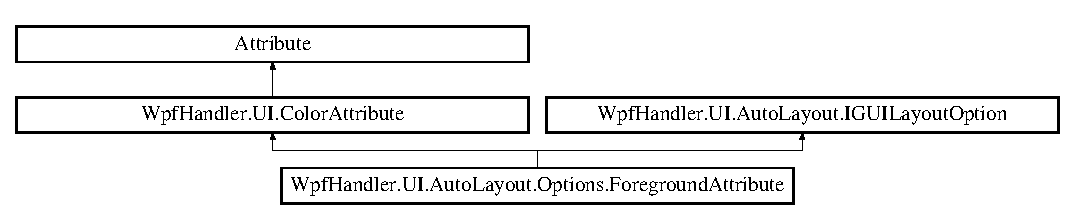
\includegraphics[height=2.507463cm]{dc/df7/class_wpf_handler_1_1_u_i_1_1_auto_layout_1_1_options_1_1_foreground_attribute}
\end{center}
\end{figure}
\subsection*{Public Member Functions}
\begin{DoxyCompactItemize}
\item 
\mbox{\hyperlink{class_wpf_handler_1_1_u_i_1_1_auto_layout_1_1_options_1_1_foreground_attribute_abae0ce13aea7130e5e9c72c208443380}{Foreground\+Attribute}} (\mbox{\hyperlink{class_wpf_handler_1_1_u_i_1_1_color_attribute_afa14c4542d8023b3ddad6aba74993877}{Brush}} brush)
\begin{DoxyCompactList}\small\item\em Instiniating attribute with applied brush. \end{DoxyCompactList}\item 
\mbox{\hyperlink{class_wpf_handler_1_1_u_i_1_1_auto_layout_1_1_options_1_1_foreground_attribute_a3c0591313938a963293a9b2df51e130b}{Foreground\+Attribute}} (Solid\+Color\+Brush brush)
\begin{DoxyCompactList}\small\item\em Instiniating attribute with applied brush. \end{DoxyCompactList}\item 
\mbox{\hyperlink{class_wpf_handler_1_1_u_i_1_1_auto_layout_1_1_options_1_1_foreground_attribute_ae4e67116f7dcce84028e700262afd1cf}{Foreground\+Attribute}} (string color\+Code)
\begin{DoxyCompactList}\small\item\em Instiniating attribute with applied brush. \end{DoxyCompactList}\item 
\mbox{\hyperlink{class_wpf_handler_1_1_u_i_1_1_auto_layout_1_1_options_1_1_foreground_attribute_ab3c65b68928d5ad4ccedee5b7baa337c}{Foreground\+Attribute}} (\mbox{\hyperlink{class_wpf_handler_1_1_u_i_1_1_color_attribute_a6c5c2202427bd48877142ecf85327843}{Color}} color)
\begin{DoxyCompactList}\small\item\em Instiniating attribute with applied color. \end{DoxyCompactList}\item 
void \mbox{\hyperlink{class_wpf_handler_1_1_u_i_1_1_auto_layout_1_1_options_1_1_foreground_attribute_a5231ed2afb4d2d26eac9eab670adca45}{Apply\+Layout\+Option}} (Framework\+Element element)
\begin{DoxyCompactList}\small\item\em Define G\+UI element\textquotesingle{}s foreground brush. \end{DoxyCompactList}\end{DoxyCompactItemize}
\subsection*{Additional Inherited Members}


\subsection{Detailed Description}
Define G\+UI element\textquotesingle{}s foreground brush. 



\subsection{Constructor \& Destructor Documentation}
\mbox{\Hypertarget{class_wpf_handler_1_1_u_i_1_1_auto_layout_1_1_options_1_1_foreground_attribute_abae0ce13aea7130e5e9c72c208443380}\label{class_wpf_handler_1_1_u_i_1_1_auto_layout_1_1_options_1_1_foreground_attribute_abae0ce13aea7130e5e9c72c208443380}} 
\index{Wpf\+Handler\+::\+U\+I\+::\+Auto\+Layout\+::\+Options\+::\+Foreground\+Attribute@{Wpf\+Handler\+::\+U\+I\+::\+Auto\+Layout\+::\+Options\+::\+Foreground\+Attribute}!Foreground\+Attribute@{Foreground\+Attribute}}
\index{Foreground\+Attribute@{Foreground\+Attribute}!Wpf\+Handler\+::\+U\+I\+::\+Auto\+Layout\+::\+Options\+::\+Foreground\+Attribute@{Wpf\+Handler\+::\+U\+I\+::\+Auto\+Layout\+::\+Options\+::\+Foreground\+Attribute}}
\subsubsection{\texorpdfstring{Foreground\+Attribute()}{ForegroundAttribute()}\hspace{0.1cm}{\footnotesize\ttfamily [1/4]}}
{\footnotesize\ttfamily Wpf\+Handler.\+U\+I.\+Auto\+Layout.\+Options.\+Foreground\+Attribute.\+Foreground\+Attribute (\begin{DoxyParamCaption}\item[{\mbox{\hyperlink{class_wpf_handler_1_1_u_i_1_1_color_attribute_afa14c4542d8023b3ddad6aba74993877}{Brush}}}]{brush }\end{DoxyParamCaption})}



Instiniating attribute with applied brush. 


\begin{DoxyParams}{Parameters}
{\em brush} & Target brush.\\
\hline
\end{DoxyParams}


No supported via attribute.\mbox{\Hypertarget{class_wpf_handler_1_1_u_i_1_1_auto_layout_1_1_options_1_1_foreground_attribute_a3c0591313938a963293a9b2df51e130b}\label{class_wpf_handler_1_1_u_i_1_1_auto_layout_1_1_options_1_1_foreground_attribute_a3c0591313938a963293a9b2df51e130b}} 
\index{Wpf\+Handler\+::\+U\+I\+::\+Auto\+Layout\+::\+Options\+::\+Foreground\+Attribute@{Wpf\+Handler\+::\+U\+I\+::\+Auto\+Layout\+::\+Options\+::\+Foreground\+Attribute}!Foreground\+Attribute@{Foreground\+Attribute}}
\index{Foreground\+Attribute@{Foreground\+Attribute}!Wpf\+Handler\+::\+U\+I\+::\+Auto\+Layout\+::\+Options\+::\+Foreground\+Attribute@{Wpf\+Handler\+::\+U\+I\+::\+Auto\+Layout\+::\+Options\+::\+Foreground\+Attribute}}
\subsubsection{\texorpdfstring{Foreground\+Attribute()}{ForegroundAttribute()}\hspace{0.1cm}{\footnotesize\ttfamily [2/4]}}
{\footnotesize\ttfamily Wpf\+Handler.\+U\+I.\+Auto\+Layout.\+Options.\+Foreground\+Attribute.\+Foreground\+Attribute (\begin{DoxyParamCaption}\item[{Solid\+Color\+Brush}]{brush }\end{DoxyParamCaption})}



Instiniating attribute with applied brush. 


\begin{DoxyParams}{Parameters}
{\em brush} & Target brush.\\
\hline
\end{DoxyParams}


No supported via attribute.\mbox{\Hypertarget{class_wpf_handler_1_1_u_i_1_1_auto_layout_1_1_options_1_1_foreground_attribute_ae4e67116f7dcce84028e700262afd1cf}\label{class_wpf_handler_1_1_u_i_1_1_auto_layout_1_1_options_1_1_foreground_attribute_ae4e67116f7dcce84028e700262afd1cf}} 
\index{Wpf\+Handler\+::\+U\+I\+::\+Auto\+Layout\+::\+Options\+::\+Foreground\+Attribute@{Wpf\+Handler\+::\+U\+I\+::\+Auto\+Layout\+::\+Options\+::\+Foreground\+Attribute}!Foreground\+Attribute@{Foreground\+Attribute}}
\index{Foreground\+Attribute@{Foreground\+Attribute}!Wpf\+Handler\+::\+U\+I\+::\+Auto\+Layout\+::\+Options\+::\+Foreground\+Attribute@{Wpf\+Handler\+::\+U\+I\+::\+Auto\+Layout\+::\+Options\+::\+Foreground\+Attribute}}
\subsubsection{\texorpdfstring{Foreground\+Attribute()}{ForegroundAttribute()}\hspace{0.1cm}{\footnotesize\ttfamily [3/4]}}
{\footnotesize\ttfamily Wpf\+Handler.\+U\+I.\+Auto\+Layout.\+Options.\+Foreground\+Attribute.\+Foreground\+Attribute (\begin{DoxyParamCaption}\item[{string}]{color\+Code }\end{DoxyParamCaption})}



Instiniating attribute with applied brush. 


\begin{DoxyParams}{Parameters}
{\em color\+Code} & Trying to apply string color code as brush by using Color\+Converter rules. Not throw excption in case if color\textquotesingle{}s code invalid to prevent \mbox{\hyperlink{namespace_wpf_handler_1_1_u_i}{UI}} crash.\\
\hline
\end{DoxyParams}
\mbox{\Hypertarget{class_wpf_handler_1_1_u_i_1_1_auto_layout_1_1_options_1_1_foreground_attribute_ab3c65b68928d5ad4ccedee5b7baa337c}\label{class_wpf_handler_1_1_u_i_1_1_auto_layout_1_1_options_1_1_foreground_attribute_ab3c65b68928d5ad4ccedee5b7baa337c}} 
\index{Wpf\+Handler\+::\+U\+I\+::\+Auto\+Layout\+::\+Options\+::\+Foreground\+Attribute@{Wpf\+Handler\+::\+U\+I\+::\+Auto\+Layout\+::\+Options\+::\+Foreground\+Attribute}!Foreground\+Attribute@{Foreground\+Attribute}}
\index{Foreground\+Attribute@{Foreground\+Attribute}!Wpf\+Handler\+::\+U\+I\+::\+Auto\+Layout\+::\+Options\+::\+Foreground\+Attribute@{Wpf\+Handler\+::\+U\+I\+::\+Auto\+Layout\+::\+Options\+::\+Foreground\+Attribute}}
\subsubsection{\texorpdfstring{Foreground\+Attribute()}{ForegroundAttribute()}\hspace{0.1cm}{\footnotesize\ttfamily [4/4]}}
{\footnotesize\ttfamily Wpf\+Handler.\+U\+I.\+Auto\+Layout.\+Options.\+Foreground\+Attribute.\+Foreground\+Attribute (\begin{DoxyParamCaption}\item[{\mbox{\hyperlink{class_wpf_handler_1_1_u_i_1_1_color_attribute_a6c5c2202427bd48877142ecf85327843}{Color}}}]{color }\end{DoxyParamCaption})}



Instiniating attribute with applied color. 


\begin{DoxyParams}{Parameters}
{\em color} & Target color.\\
\hline
\end{DoxyParams}


No supported via attribute.

\subsection{Member Function Documentation}
\mbox{\Hypertarget{class_wpf_handler_1_1_u_i_1_1_auto_layout_1_1_options_1_1_foreground_attribute_a5231ed2afb4d2d26eac9eab670adca45}\label{class_wpf_handler_1_1_u_i_1_1_auto_layout_1_1_options_1_1_foreground_attribute_a5231ed2afb4d2d26eac9eab670adca45}} 
\index{Wpf\+Handler\+::\+U\+I\+::\+Auto\+Layout\+::\+Options\+::\+Foreground\+Attribute@{Wpf\+Handler\+::\+U\+I\+::\+Auto\+Layout\+::\+Options\+::\+Foreground\+Attribute}!Apply\+Layout\+Option@{Apply\+Layout\+Option}}
\index{Apply\+Layout\+Option@{Apply\+Layout\+Option}!Wpf\+Handler\+::\+U\+I\+::\+Auto\+Layout\+::\+Options\+::\+Foreground\+Attribute@{Wpf\+Handler\+::\+U\+I\+::\+Auto\+Layout\+::\+Options\+::\+Foreground\+Attribute}}
\subsubsection{\texorpdfstring{Apply\+Layout\+Option()}{ApplyLayoutOption()}}
{\footnotesize\ttfamily void Wpf\+Handler.\+U\+I.\+Auto\+Layout.\+Options.\+Foreground\+Attribute.\+Apply\+Layout\+Option (\begin{DoxyParamCaption}\item[{Framework\+Element}]{element }\end{DoxyParamCaption})}



Define G\+UI element\textquotesingle{}s foreground brush. 


\begin{DoxyParams}{Parameters}
{\em element} & Shared \mbox{\hyperlink{namespace_wpf_handler_1_1_u_i}{UI}} element. Must be inheirted from {\ttfamily System.\+Windows.\+Controls.\+Control} to affect the font properties. \\
\hline
\end{DoxyParams}


Implements \mbox{\hyperlink{interface_wpf_handler_1_1_u_i_1_1_auto_layout_1_1_i_g_u_i_layout_option_ac2d2fa8aeaf753b3248381399f991005}{Wpf\+Handler.\+U\+I.\+Auto\+Layout.\+I\+G\+U\+I\+Layout\+Option}}.



The documentation for this class was generated from the following file\+:\begin{DoxyCompactItemize}
\item 
D\+:/\+Work/\+Git\+Hub/wpf-\/handler/\+Wpf\+Handler/\+U\+I/\+Auto\+Layout/\+Options/Foreground\+Attribute.\+cs\end{DoxyCompactItemize}

\hypertarget{class_wpf_handler_1_1_u_i_1_1_auto_layout_1_1_form_descriptor}{}\section{Wpf\+Handler.\+U\+I.\+Auto\+Layout.\+Form\+Descriptor Class Reference}
\label{class_wpf_handler_1_1_u_i_1_1_auto_layout_1_1_form_descriptor}\index{Wpf\+Handler.\+U\+I.\+Auto\+Layout.\+Form\+Descriptor@{Wpf\+Handler.\+U\+I.\+Auto\+Layout.\+Form\+Descriptor}}


An abstract \mbox{\hyperlink{namespace_wpf_handler_1_1_u_i}{UI}} descriptor suitable for the form-\/like interfaces.  


Inheritance diagram for Wpf\+Handler.\+U\+I.\+Auto\+Layout.\+Form\+Descriptor\+:\begin{figure}[H]
\begin{center}
\leavevmode
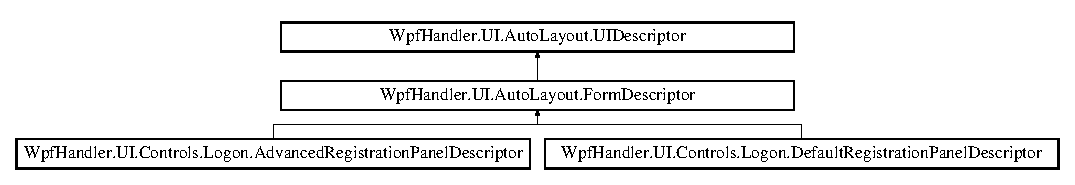
\includegraphics[height=2.043796cm]{d9/d42/class_wpf_handler_1_1_u_i_1_1_auto_layout_1_1_form_descriptor}
\end{center}
\end{figure}
\subsection*{Classes}
\begin{DoxyCompactItemize}
\item 
struct \mbox{\hyperlink{struct_wpf_handler_1_1_u_i_1_1_auto_layout_1_1_form_descriptor_1_1_validation_report}{Validation\+Report}}
\begin{DoxyCompactList}\small\item\em Sturcture that contains a validation report data. \end{DoxyCompactList}\end{DoxyCompactItemize}
\subsection*{Public Member Functions}
\begin{DoxyCompactItemize}
\item 
virtual \mbox{\hyperlink{struct_wpf_handler_1_1_u_i_1_1_auto_layout_1_1_form_descriptor_1_1_validation_report}{Validation\+Report}} \mbox{\hyperlink{class_wpf_handler_1_1_u_i_1_1_auto_layout_1_1_form_descriptor_a63527cbe3f75e544b7f4ab417bfbb555}{On\+Validation}} ()
\begin{DoxyCompactList}\small\item\em Handelr that will be called when a from should validate members data. \end{DoxyCompactList}\item 
virtual void \mbox{\hyperlink{class_wpf_handler_1_1_u_i_1_1_auto_layout_1_1_form_descriptor_ae2d4791e3085dba435c09b6082bd8408}{On\+Confirm}} ()
\begin{DoxyCompactList}\small\item\em A handler that will called when the form will be confirmed. Handle the stored data. \end{DoxyCompactList}\item 
virtual void \mbox{\hyperlink{class_wpf_handler_1_1_u_i_1_1_auto_layout_1_1_form_descriptor_a4bbe131238be232c253ca4c65e8493f4}{On\+Cancel}} ()
\begin{DoxyCompactList}\small\item\em A handler that will called when the form will be canceled. Handle the stored data. \end{DoxyCompactList}\end{DoxyCompactItemize}
\subsection*{Events}
\begin{DoxyCompactItemize}
\item 
Action$<$ \mbox{\hyperlink{class_wpf_handler_1_1_u_i_1_1_auto_layout_1_1_form_descriptor}{Form\+Descriptor}} $>$ \mbox{\hyperlink{class_wpf_handler_1_1_u_i_1_1_auto_layout_1_1_form_descriptor_a8a95b91b04aec2b3e109845866c25fb2}{On\+Confirm\+Event}}
\begin{DoxyCompactList}\small\item\em Occurs avter calling the \mbox{\hyperlink{class_wpf_handler_1_1_u_i_1_1_auto_layout_1_1_form_descriptor_ae2d4791e3085dba435c09b6082bd8408}{On\+Confirm}} handler. \end{DoxyCompactList}\item 
Action$<$ \mbox{\hyperlink{class_wpf_handler_1_1_u_i_1_1_auto_layout_1_1_form_descriptor}{Form\+Descriptor}} $>$ \mbox{\hyperlink{class_wpf_handler_1_1_u_i_1_1_auto_layout_1_1_form_descriptor_a5be99456050a10453139bf7a27baa78a}{On\+Cancel\+Event}}
\begin{DoxyCompactList}\small\item\em Occurs avter calling the \mbox{\hyperlink{class_wpf_handler_1_1_u_i_1_1_auto_layout_1_1_form_descriptor_a4bbe131238be232c253ca4c65e8493f4}{On\+Cancel}} handler. \end{DoxyCompactList}\end{DoxyCompactItemize}
\subsection*{Additional Inherited Members}


\subsection{Detailed Description}
An abstract \mbox{\hyperlink{namespace_wpf_handler_1_1_u_i}{UI}} descriptor suitable for the form-\/like interfaces. 



\subsection{Member Function Documentation}
\mbox{\Hypertarget{class_wpf_handler_1_1_u_i_1_1_auto_layout_1_1_form_descriptor_a4bbe131238be232c253ca4c65e8493f4}\label{class_wpf_handler_1_1_u_i_1_1_auto_layout_1_1_form_descriptor_a4bbe131238be232c253ca4c65e8493f4}} 
\index{Wpf\+Handler\+::\+U\+I\+::\+Auto\+Layout\+::\+Form\+Descriptor@{Wpf\+Handler\+::\+U\+I\+::\+Auto\+Layout\+::\+Form\+Descriptor}!On\+Cancel@{On\+Cancel}}
\index{On\+Cancel@{On\+Cancel}!Wpf\+Handler\+::\+U\+I\+::\+Auto\+Layout\+::\+Form\+Descriptor@{Wpf\+Handler\+::\+U\+I\+::\+Auto\+Layout\+::\+Form\+Descriptor}}
\subsubsection{\texorpdfstring{On\+Cancel()}{OnCancel()}}
{\footnotesize\ttfamily virtual void Wpf\+Handler.\+U\+I.\+Auto\+Layout.\+Form\+Descriptor.\+On\+Cancel (\begin{DoxyParamCaption}{ }\end{DoxyParamCaption})\hspace{0.3cm}{\ttfamily [virtual]}}



A handler that will called when the form will be canceled. Handle the stored data. 



Reimplemented in \mbox{\hyperlink{class_wpf_handler_1_1_u_i_1_1_controls_1_1_logon_1_1_default_registration_panel_descriptor_a9154a1e27afdf8d40da139042ee7e609}{Wpf\+Handler.\+U\+I.\+Controls.\+Logon.\+Default\+Registration\+Panel\+Descriptor}}.

\mbox{\Hypertarget{class_wpf_handler_1_1_u_i_1_1_auto_layout_1_1_form_descriptor_ae2d4791e3085dba435c09b6082bd8408}\label{class_wpf_handler_1_1_u_i_1_1_auto_layout_1_1_form_descriptor_ae2d4791e3085dba435c09b6082bd8408}} 
\index{Wpf\+Handler\+::\+U\+I\+::\+Auto\+Layout\+::\+Form\+Descriptor@{Wpf\+Handler\+::\+U\+I\+::\+Auto\+Layout\+::\+Form\+Descriptor}!On\+Confirm@{On\+Confirm}}
\index{On\+Confirm@{On\+Confirm}!Wpf\+Handler\+::\+U\+I\+::\+Auto\+Layout\+::\+Form\+Descriptor@{Wpf\+Handler\+::\+U\+I\+::\+Auto\+Layout\+::\+Form\+Descriptor}}
\subsubsection{\texorpdfstring{On\+Confirm()}{OnConfirm()}}
{\footnotesize\ttfamily virtual void Wpf\+Handler.\+U\+I.\+Auto\+Layout.\+Form\+Descriptor.\+On\+Confirm (\begin{DoxyParamCaption}{ }\end{DoxyParamCaption})\hspace{0.3cm}{\ttfamily [virtual]}}



A handler that will called when the form will be confirmed. Handle the stored data. 



Reimplemented in \mbox{\hyperlink{class_wpf_handler_1_1_u_i_1_1_controls_1_1_logon_1_1_default_registration_panel_descriptor_aee1e6b6ba9214aac4a82b0213e4d3442}{Wpf\+Handler.\+U\+I.\+Controls.\+Logon.\+Default\+Registration\+Panel\+Descriptor}}.

\mbox{\Hypertarget{class_wpf_handler_1_1_u_i_1_1_auto_layout_1_1_form_descriptor_a63527cbe3f75e544b7f4ab417bfbb555}\label{class_wpf_handler_1_1_u_i_1_1_auto_layout_1_1_form_descriptor_a63527cbe3f75e544b7f4ab417bfbb555}} 
\index{Wpf\+Handler\+::\+U\+I\+::\+Auto\+Layout\+::\+Form\+Descriptor@{Wpf\+Handler\+::\+U\+I\+::\+Auto\+Layout\+::\+Form\+Descriptor}!On\+Validation@{On\+Validation}}
\index{On\+Validation@{On\+Validation}!Wpf\+Handler\+::\+U\+I\+::\+Auto\+Layout\+::\+Form\+Descriptor@{Wpf\+Handler\+::\+U\+I\+::\+Auto\+Layout\+::\+Form\+Descriptor}}
\subsubsection{\texorpdfstring{On\+Validation()}{OnValidation()}}
{\footnotesize\ttfamily virtual \mbox{\hyperlink{struct_wpf_handler_1_1_u_i_1_1_auto_layout_1_1_form_descriptor_1_1_validation_report}{Validation\+Report}} Wpf\+Handler.\+U\+I.\+Auto\+Layout.\+Form\+Descriptor.\+On\+Validation (\begin{DoxyParamCaption}{ }\end{DoxyParamCaption})\hspace{0.3cm}{\ttfamily [virtual]}}



Handelr that will be called when a from should validate members data. 

\begin{DoxyReturn}{Returns}
A validation report. 
\end{DoxyReturn}


Reimplemented in \mbox{\hyperlink{class_wpf_handler_1_1_u_i_1_1_controls_1_1_logon_1_1_default_registration_panel_descriptor_abc8055d00358a941e9b507fed58ff662}{Wpf\+Handler.\+U\+I.\+Controls.\+Logon.\+Default\+Registration\+Panel\+Descriptor}}.



\subsection{Event Documentation}
\mbox{\Hypertarget{class_wpf_handler_1_1_u_i_1_1_auto_layout_1_1_form_descriptor_a5be99456050a10453139bf7a27baa78a}\label{class_wpf_handler_1_1_u_i_1_1_auto_layout_1_1_form_descriptor_a5be99456050a10453139bf7a27baa78a}} 
\index{Wpf\+Handler\+::\+U\+I\+::\+Auto\+Layout\+::\+Form\+Descriptor@{Wpf\+Handler\+::\+U\+I\+::\+Auto\+Layout\+::\+Form\+Descriptor}!On\+Cancel\+Event@{On\+Cancel\+Event}}
\index{On\+Cancel\+Event@{On\+Cancel\+Event}!Wpf\+Handler\+::\+U\+I\+::\+Auto\+Layout\+::\+Form\+Descriptor@{Wpf\+Handler\+::\+U\+I\+::\+Auto\+Layout\+::\+Form\+Descriptor}}
\subsubsection{\texorpdfstring{On\+Cancel\+Event}{OnCancelEvent}}
{\footnotesize\ttfamily Action$<$\mbox{\hyperlink{class_wpf_handler_1_1_u_i_1_1_auto_layout_1_1_form_descriptor}{Form\+Descriptor}}$>$ Wpf\+Handler.\+U\+I.\+Auto\+Layout.\+Form\+Descriptor.\+On\+Cancel\+Event}



Occurs avter calling the \mbox{\hyperlink{class_wpf_handler_1_1_u_i_1_1_auto_layout_1_1_form_descriptor_a4bbe131238be232c253ca4c65e8493f4}{On\+Cancel}} handler. 

\mbox{\Hypertarget{class_wpf_handler_1_1_u_i_1_1_auto_layout_1_1_form_descriptor_a8a95b91b04aec2b3e109845866c25fb2}\label{class_wpf_handler_1_1_u_i_1_1_auto_layout_1_1_form_descriptor_a8a95b91b04aec2b3e109845866c25fb2}} 
\index{Wpf\+Handler\+::\+U\+I\+::\+Auto\+Layout\+::\+Form\+Descriptor@{Wpf\+Handler\+::\+U\+I\+::\+Auto\+Layout\+::\+Form\+Descriptor}!On\+Confirm\+Event@{On\+Confirm\+Event}}
\index{On\+Confirm\+Event@{On\+Confirm\+Event}!Wpf\+Handler\+::\+U\+I\+::\+Auto\+Layout\+::\+Form\+Descriptor@{Wpf\+Handler\+::\+U\+I\+::\+Auto\+Layout\+::\+Form\+Descriptor}}
\subsubsection{\texorpdfstring{On\+Confirm\+Event}{OnConfirmEvent}}
{\footnotesize\ttfamily Action$<$\mbox{\hyperlink{class_wpf_handler_1_1_u_i_1_1_auto_layout_1_1_form_descriptor}{Form\+Descriptor}}$>$ Wpf\+Handler.\+U\+I.\+Auto\+Layout.\+Form\+Descriptor.\+On\+Confirm\+Event}



Occurs avter calling the \mbox{\hyperlink{class_wpf_handler_1_1_u_i_1_1_auto_layout_1_1_form_descriptor_ae2d4791e3085dba435c09b6082bd8408}{On\+Confirm}} handler. 



The documentation for this class was generated from the following file\+:\begin{DoxyCompactItemize}
\item 
D\+:/\+Work/\+Git\+Hub/wpf-\/handler/\+Wpf\+Handler/\+U\+I/\+Auto\+Layout/Form\+Descriptor.\+cs\end{DoxyCompactItemize}

\hypertarget{class_xaml_generated_namespace_1_1_generated_internal_type_helper}{}\section{Xaml\+Generated\+Namespace.\+Generated\+Internal\+Type\+Helper Class Reference}
\label{class_xaml_generated_namespace_1_1_generated_internal_type_helper}\index{Xaml\+Generated\+Namespace.\+Generated\+Internal\+Type\+Helper@{Xaml\+Generated\+Namespace.\+Generated\+Internal\+Type\+Helper}}


\mbox{\hyperlink{class_xaml_generated_namespace_1_1_generated_internal_type_helper}{Generated\+Internal\+Type\+Helper}}  


Inheritance diagram for Xaml\+Generated\+Namespace.\+Generated\+Internal\+Type\+Helper\+:\begin{figure}[H]
\begin{center}
\leavevmode
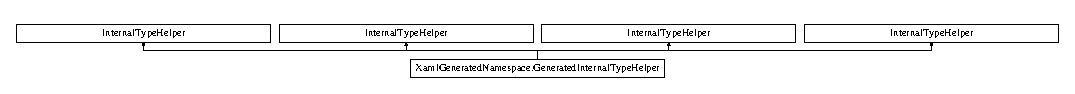
\includegraphics[height=0.813953cm]{dc/db0/class_xaml_generated_namespace_1_1_generated_internal_type_helper}
\end{center}
\end{figure}
\subsection*{Protected Member Functions}
\begin{DoxyCompactItemize}
\item 
override object \mbox{\hyperlink{class_xaml_generated_namespace_1_1_generated_internal_type_helper_aefb7a98fceb9c287cef4756942f441d1}{Create\+Instance}} (System.\+Type type, System.\+Globalization.\+Culture\+Info culture)
\begin{DoxyCompactList}\small\item\em Create\+Instance \end{DoxyCompactList}\item 
override object \mbox{\hyperlink{class_xaml_generated_namespace_1_1_generated_internal_type_helper_afdc9fe15b56607d02082908d934480c6}{Get\+Property\+Value}} (System.\+Reflection.\+Property\+Info property\+Info, object target, System.\+Globalization.\+Culture\+Info culture)
\begin{DoxyCompactList}\small\item\em Get\+Property\+Value \end{DoxyCompactList}\item 
override void \mbox{\hyperlink{class_xaml_generated_namespace_1_1_generated_internal_type_helper_ade0f04c0f7b18dd5b170e071d5534d38}{Set\+Property\+Value}} (System.\+Reflection.\+Property\+Info property\+Info, object target, object value, System.\+Globalization.\+Culture\+Info culture)
\begin{DoxyCompactList}\small\item\em Set\+Property\+Value \end{DoxyCompactList}\item 
override System.\+Delegate \mbox{\hyperlink{class_xaml_generated_namespace_1_1_generated_internal_type_helper_a8ec4c37e82d9f4e867e9655f4eac3a78}{Create\+Delegate}} (System.\+Type delegate\+Type, object target, string handler)
\begin{DoxyCompactList}\small\item\em Create\+Delegate \end{DoxyCompactList}\item 
override void \mbox{\hyperlink{class_xaml_generated_namespace_1_1_generated_internal_type_helper_a73471f4a6d1ca4c4fceec9ad8610f0c8}{Add\+Event\+Handler}} (System.\+Reflection.\+Event\+Info event\+Info, object target, System.\+Delegate handler)
\begin{DoxyCompactList}\small\item\em Add\+Event\+Handler \end{DoxyCompactList}\item 
override object \mbox{\hyperlink{class_xaml_generated_namespace_1_1_generated_internal_type_helper_aefb7a98fceb9c287cef4756942f441d1}{Create\+Instance}} (System.\+Type type, System.\+Globalization.\+Culture\+Info culture)
\begin{DoxyCompactList}\small\item\em Create\+Instance \end{DoxyCompactList}\item 
override object \mbox{\hyperlink{class_xaml_generated_namespace_1_1_generated_internal_type_helper_afdc9fe15b56607d02082908d934480c6}{Get\+Property\+Value}} (System.\+Reflection.\+Property\+Info property\+Info, object target, System.\+Globalization.\+Culture\+Info culture)
\begin{DoxyCompactList}\small\item\em Get\+Property\+Value \end{DoxyCompactList}\item 
override void \mbox{\hyperlink{class_xaml_generated_namespace_1_1_generated_internal_type_helper_ade0f04c0f7b18dd5b170e071d5534d38}{Set\+Property\+Value}} (System.\+Reflection.\+Property\+Info property\+Info, object target, object value, System.\+Globalization.\+Culture\+Info culture)
\begin{DoxyCompactList}\small\item\em Set\+Property\+Value \end{DoxyCompactList}\item 
override System.\+Delegate \mbox{\hyperlink{class_xaml_generated_namespace_1_1_generated_internal_type_helper_a8ec4c37e82d9f4e867e9655f4eac3a78}{Create\+Delegate}} (System.\+Type delegate\+Type, object target, string handler)
\begin{DoxyCompactList}\small\item\em Create\+Delegate \end{DoxyCompactList}\item 
override void \mbox{\hyperlink{class_xaml_generated_namespace_1_1_generated_internal_type_helper_a73471f4a6d1ca4c4fceec9ad8610f0c8}{Add\+Event\+Handler}} (System.\+Reflection.\+Event\+Info event\+Info, object target, System.\+Delegate handler)
\begin{DoxyCompactList}\small\item\em Add\+Event\+Handler \end{DoxyCompactList}\item 
override object \mbox{\hyperlink{class_xaml_generated_namespace_1_1_generated_internal_type_helper_aefb7a98fceb9c287cef4756942f441d1}{Create\+Instance}} (System.\+Type type, System.\+Globalization.\+Culture\+Info culture)
\begin{DoxyCompactList}\small\item\em Create\+Instance \end{DoxyCompactList}\item 
override object \mbox{\hyperlink{class_xaml_generated_namespace_1_1_generated_internal_type_helper_afdc9fe15b56607d02082908d934480c6}{Get\+Property\+Value}} (System.\+Reflection.\+Property\+Info property\+Info, object target, System.\+Globalization.\+Culture\+Info culture)
\begin{DoxyCompactList}\small\item\em Get\+Property\+Value \end{DoxyCompactList}\item 
override void \mbox{\hyperlink{class_xaml_generated_namespace_1_1_generated_internal_type_helper_ade0f04c0f7b18dd5b170e071d5534d38}{Set\+Property\+Value}} (System.\+Reflection.\+Property\+Info property\+Info, object target, object value, System.\+Globalization.\+Culture\+Info culture)
\begin{DoxyCompactList}\small\item\em Set\+Property\+Value \end{DoxyCompactList}\item 
override System.\+Delegate \mbox{\hyperlink{class_xaml_generated_namespace_1_1_generated_internal_type_helper_a8ec4c37e82d9f4e867e9655f4eac3a78}{Create\+Delegate}} (System.\+Type delegate\+Type, object target, string handler)
\begin{DoxyCompactList}\small\item\em Create\+Delegate \end{DoxyCompactList}\item 
override void \mbox{\hyperlink{class_xaml_generated_namespace_1_1_generated_internal_type_helper_a73471f4a6d1ca4c4fceec9ad8610f0c8}{Add\+Event\+Handler}} (System.\+Reflection.\+Event\+Info event\+Info, object target, System.\+Delegate handler)
\begin{DoxyCompactList}\small\item\em Add\+Event\+Handler \end{DoxyCompactList}\item 
override object \mbox{\hyperlink{class_xaml_generated_namespace_1_1_generated_internal_type_helper_aefb7a98fceb9c287cef4756942f441d1}{Create\+Instance}} (System.\+Type type, System.\+Globalization.\+Culture\+Info culture)
\begin{DoxyCompactList}\small\item\em Create\+Instance \end{DoxyCompactList}\item 
override object \mbox{\hyperlink{class_xaml_generated_namespace_1_1_generated_internal_type_helper_afdc9fe15b56607d02082908d934480c6}{Get\+Property\+Value}} (System.\+Reflection.\+Property\+Info property\+Info, object target, System.\+Globalization.\+Culture\+Info culture)
\begin{DoxyCompactList}\small\item\em Get\+Property\+Value \end{DoxyCompactList}\item 
override void \mbox{\hyperlink{class_xaml_generated_namespace_1_1_generated_internal_type_helper_ade0f04c0f7b18dd5b170e071d5534d38}{Set\+Property\+Value}} (System.\+Reflection.\+Property\+Info property\+Info, object target, object value, System.\+Globalization.\+Culture\+Info culture)
\begin{DoxyCompactList}\small\item\em Set\+Property\+Value \end{DoxyCompactList}\item 
override System.\+Delegate \mbox{\hyperlink{class_xaml_generated_namespace_1_1_generated_internal_type_helper_a8ec4c37e82d9f4e867e9655f4eac3a78}{Create\+Delegate}} (System.\+Type delegate\+Type, object target, string handler)
\begin{DoxyCompactList}\small\item\em Create\+Delegate \end{DoxyCompactList}\item 
override void \mbox{\hyperlink{class_xaml_generated_namespace_1_1_generated_internal_type_helper_a73471f4a6d1ca4c4fceec9ad8610f0c8}{Add\+Event\+Handler}} (System.\+Reflection.\+Event\+Info event\+Info, object target, System.\+Delegate handler)
\begin{DoxyCompactList}\small\item\em Add\+Event\+Handler \end{DoxyCompactList}\end{DoxyCompactItemize}


\subsection{Detailed Description}
\mbox{\hyperlink{class_xaml_generated_namespace_1_1_generated_internal_type_helper}{Generated\+Internal\+Type\+Helper}} 



\subsection{Member Function Documentation}
\mbox{\Hypertarget{class_xaml_generated_namespace_1_1_generated_internal_type_helper_a73471f4a6d1ca4c4fceec9ad8610f0c8}\label{class_xaml_generated_namespace_1_1_generated_internal_type_helper_a73471f4a6d1ca4c4fceec9ad8610f0c8}} 
\index{Xaml\+Generated\+Namespace\+::\+Generated\+Internal\+Type\+Helper@{Xaml\+Generated\+Namespace\+::\+Generated\+Internal\+Type\+Helper}!Add\+Event\+Handler@{Add\+Event\+Handler}}
\index{Add\+Event\+Handler@{Add\+Event\+Handler}!Xaml\+Generated\+Namespace\+::\+Generated\+Internal\+Type\+Helper@{Xaml\+Generated\+Namespace\+::\+Generated\+Internal\+Type\+Helper}}
\subsubsection{\texorpdfstring{Add\+Event\+Handler()}{AddEventHandler()}\hspace{0.1cm}{\footnotesize\ttfamily [1/4]}}
{\footnotesize\ttfamily override void Xaml\+Generated\+Namespace.\+Generated\+Internal\+Type\+Helper.\+Add\+Event\+Handler (\begin{DoxyParamCaption}\item[{System.\+Reflection.\+Event\+Info}]{event\+Info,  }\item[{object}]{target,  }\item[{System.\+Delegate}]{handler }\end{DoxyParamCaption})\hspace{0.3cm}{\ttfamily [protected]}}



Add\+Event\+Handler 

\mbox{\Hypertarget{class_xaml_generated_namespace_1_1_generated_internal_type_helper_a73471f4a6d1ca4c4fceec9ad8610f0c8}\label{class_xaml_generated_namespace_1_1_generated_internal_type_helper_a73471f4a6d1ca4c4fceec9ad8610f0c8}} 
\index{Xaml\+Generated\+Namespace\+::\+Generated\+Internal\+Type\+Helper@{Xaml\+Generated\+Namespace\+::\+Generated\+Internal\+Type\+Helper}!Add\+Event\+Handler@{Add\+Event\+Handler}}
\index{Add\+Event\+Handler@{Add\+Event\+Handler}!Xaml\+Generated\+Namespace\+::\+Generated\+Internal\+Type\+Helper@{Xaml\+Generated\+Namespace\+::\+Generated\+Internal\+Type\+Helper}}
\subsubsection{\texorpdfstring{Add\+Event\+Handler()}{AddEventHandler()}\hspace{0.1cm}{\footnotesize\ttfamily [2/4]}}
{\footnotesize\ttfamily override void Xaml\+Generated\+Namespace.\+Generated\+Internal\+Type\+Helper.\+Add\+Event\+Handler (\begin{DoxyParamCaption}\item[{System.\+Reflection.\+Event\+Info}]{event\+Info,  }\item[{object}]{target,  }\item[{System.\+Delegate}]{handler }\end{DoxyParamCaption})\hspace{0.3cm}{\ttfamily [protected]}}



Add\+Event\+Handler 

\mbox{\Hypertarget{class_xaml_generated_namespace_1_1_generated_internal_type_helper_a73471f4a6d1ca4c4fceec9ad8610f0c8}\label{class_xaml_generated_namespace_1_1_generated_internal_type_helper_a73471f4a6d1ca4c4fceec9ad8610f0c8}} 
\index{Xaml\+Generated\+Namespace\+::\+Generated\+Internal\+Type\+Helper@{Xaml\+Generated\+Namespace\+::\+Generated\+Internal\+Type\+Helper}!Add\+Event\+Handler@{Add\+Event\+Handler}}
\index{Add\+Event\+Handler@{Add\+Event\+Handler}!Xaml\+Generated\+Namespace\+::\+Generated\+Internal\+Type\+Helper@{Xaml\+Generated\+Namespace\+::\+Generated\+Internal\+Type\+Helper}}
\subsubsection{\texorpdfstring{Add\+Event\+Handler()}{AddEventHandler()}\hspace{0.1cm}{\footnotesize\ttfamily [3/4]}}
{\footnotesize\ttfamily override void Xaml\+Generated\+Namespace.\+Generated\+Internal\+Type\+Helper.\+Add\+Event\+Handler (\begin{DoxyParamCaption}\item[{System.\+Reflection.\+Event\+Info}]{event\+Info,  }\item[{object}]{target,  }\item[{System.\+Delegate}]{handler }\end{DoxyParamCaption})\hspace{0.3cm}{\ttfamily [protected]}}



Add\+Event\+Handler 

\mbox{\Hypertarget{class_xaml_generated_namespace_1_1_generated_internal_type_helper_a73471f4a6d1ca4c4fceec9ad8610f0c8}\label{class_xaml_generated_namespace_1_1_generated_internal_type_helper_a73471f4a6d1ca4c4fceec9ad8610f0c8}} 
\index{Xaml\+Generated\+Namespace\+::\+Generated\+Internal\+Type\+Helper@{Xaml\+Generated\+Namespace\+::\+Generated\+Internal\+Type\+Helper}!Add\+Event\+Handler@{Add\+Event\+Handler}}
\index{Add\+Event\+Handler@{Add\+Event\+Handler}!Xaml\+Generated\+Namespace\+::\+Generated\+Internal\+Type\+Helper@{Xaml\+Generated\+Namespace\+::\+Generated\+Internal\+Type\+Helper}}
\subsubsection{\texorpdfstring{Add\+Event\+Handler()}{AddEventHandler()}\hspace{0.1cm}{\footnotesize\ttfamily [4/4]}}
{\footnotesize\ttfamily override void Xaml\+Generated\+Namespace.\+Generated\+Internal\+Type\+Helper.\+Add\+Event\+Handler (\begin{DoxyParamCaption}\item[{System.\+Reflection.\+Event\+Info}]{event\+Info,  }\item[{object}]{target,  }\item[{System.\+Delegate}]{handler }\end{DoxyParamCaption})\hspace{0.3cm}{\ttfamily [protected]}}



Add\+Event\+Handler 

\mbox{\Hypertarget{class_xaml_generated_namespace_1_1_generated_internal_type_helper_a8ec4c37e82d9f4e867e9655f4eac3a78}\label{class_xaml_generated_namespace_1_1_generated_internal_type_helper_a8ec4c37e82d9f4e867e9655f4eac3a78}} 
\index{Xaml\+Generated\+Namespace\+::\+Generated\+Internal\+Type\+Helper@{Xaml\+Generated\+Namespace\+::\+Generated\+Internal\+Type\+Helper}!Create\+Delegate@{Create\+Delegate}}
\index{Create\+Delegate@{Create\+Delegate}!Xaml\+Generated\+Namespace\+::\+Generated\+Internal\+Type\+Helper@{Xaml\+Generated\+Namespace\+::\+Generated\+Internal\+Type\+Helper}}
\subsubsection{\texorpdfstring{Create\+Delegate()}{CreateDelegate()}\hspace{0.1cm}{\footnotesize\ttfamily [1/4]}}
{\footnotesize\ttfamily override System.\+Delegate Xaml\+Generated\+Namespace.\+Generated\+Internal\+Type\+Helper.\+Create\+Delegate (\begin{DoxyParamCaption}\item[{System.\+Type}]{delegate\+Type,  }\item[{object}]{target,  }\item[{string}]{handler }\end{DoxyParamCaption})\hspace{0.3cm}{\ttfamily [protected]}}



Create\+Delegate 

\mbox{\Hypertarget{class_xaml_generated_namespace_1_1_generated_internal_type_helper_a8ec4c37e82d9f4e867e9655f4eac3a78}\label{class_xaml_generated_namespace_1_1_generated_internal_type_helper_a8ec4c37e82d9f4e867e9655f4eac3a78}} 
\index{Xaml\+Generated\+Namespace\+::\+Generated\+Internal\+Type\+Helper@{Xaml\+Generated\+Namespace\+::\+Generated\+Internal\+Type\+Helper}!Create\+Delegate@{Create\+Delegate}}
\index{Create\+Delegate@{Create\+Delegate}!Xaml\+Generated\+Namespace\+::\+Generated\+Internal\+Type\+Helper@{Xaml\+Generated\+Namespace\+::\+Generated\+Internal\+Type\+Helper}}
\subsubsection{\texorpdfstring{Create\+Delegate()}{CreateDelegate()}\hspace{0.1cm}{\footnotesize\ttfamily [2/4]}}
{\footnotesize\ttfamily override System.\+Delegate Xaml\+Generated\+Namespace.\+Generated\+Internal\+Type\+Helper.\+Create\+Delegate (\begin{DoxyParamCaption}\item[{System.\+Type}]{delegate\+Type,  }\item[{object}]{target,  }\item[{string}]{handler }\end{DoxyParamCaption})\hspace{0.3cm}{\ttfamily [protected]}}



Create\+Delegate 

\mbox{\Hypertarget{class_xaml_generated_namespace_1_1_generated_internal_type_helper_a8ec4c37e82d9f4e867e9655f4eac3a78}\label{class_xaml_generated_namespace_1_1_generated_internal_type_helper_a8ec4c37e82d9f4e867e9655f4eac3a78}} 
\index{Xaml\+Generated\+Namespace\+::\+Generated\+Internal\+Type\+Helper@{Xaml\+Generated\+Namespace\+::\+Generated\+Internal\+Type\+Helper}!Create\+Delegate@{Create\+Delegate}}
\index{Create\+Delegate@{Create\+Delegate}!Xaml\+Generated\+Namespace\+::\+Generated\+Internal\+Type\+Helper@{Xaml\+Generated\+Namespace\+::\+Generated\+Internal\+Type\+Helper}}
\subsubsection{\texorpdfstring{Create\+Delegate()}{CreateDelegate()}\hspace{0.1cm}{\footnotesize\ttfamily [3/4]}}
{\footnotesize\ttfamily override System.\+Delegate Xaml\+Generated\+Namespace.\+Generated\+Internal\+Type\+Helper.\+Create\+Delegate (\begin{DoxyParamCaption}\item[{System.\+Type}]{delegate\+Type,  }\item[{object}]{target,  }\item[{string}]{handler }\end{DoxyParamCaption})\hspace{0.3cm}{\ttfamily [protected]}}



Create\+Delegate 

\mbox{\Hypertarget{class_xaml_generated_namespace_1_1_generated_internal_type_helper_a8ec4c37e82d9f4e867e9655f4eac3a78}\label{class_xaml_generated_namespace_1_1_generated_internal_type_helper_a8ec4c37e82d9f4e867e9655f4eac3a78}} 
\index{Xaml\+Generated\+Namespace\+::\+Generated\+Internal\+Type\+Helper@{Xaml\+Generated\+Namespace\+::\+Generated\+Internal\+Type\+Helper}!Create\+Delegate@{Create\+Delegate}}
\index{Create\+Delegate@{Create\+Delegate}!Xaml\+Generated\+Namespace\+::\+Generated\+Internal\+Type\+Helper@{Xaml\+Generated\+Namespace\+::\+Generated\+Internal\+Type\+Helper}}
\subsubsection{\texorpdfstring{Create\+Delegate()}{CreateDelegate()}\hspace{0.1cm}{\footnotesize\ttfamily [4/4]}}
{\footnotesize\ttfamily override System.\+Delegate Xaml\+Generated\+Namespace.\+Generated\+Internal\+Type\+Helper.\+Create\+Delegate (\begin{DoxyParamCaption}\item[{System.\+Type}]{delegate\+Type,  }\item[{object}]{target,  }\item[{string}]{handler }\end{DoxyParamCaption})\hspace{0.3cm}{\ttfamily [protected]}}



Create\+Delegate 

\mbox{\Hypertarget{class_xaml_generated_namespace_1_1_generated_internal_type_helper_aefb7a98fceb9c287cef4756942f441d1}\label{class_xaml_generated_namespace_1_1_generated_internal_type_helper_aefb7a98fceb9c287cef4756942f441d1}} 
\index{Xaml\+Generated\+Namespace\+::\+Generated\+Internal\+Type\+Helper@{Xaml\+Generated\+Namespace\+::\+Generated\+Internal\+Type\+Helper}!Create\+Instance@{Create\+Instance}}
\index{Create\+Instance@{Create\+Instance}!Xaml\+Generated\+Namespace\+::\+Generated\+Internal\+Type\+Helper@{Xaml\+Generated\+Namespace\+::\+Generated\+Internal\+Type\+Helper}}
\subsubsection{\texorpdfstring{Create\+Instance()}{CreateInstance()}\hspace{0.1cm}{\footnotesize\ttfamily [1/4]}}
{\footnotesize\ttfamily override object Xaml\+Generated\+Namespace.\+Generated\+Internal\+Type\+Helper.\+Create\+Instance (\begin{DoxyParamCaption}\item[{System.\+Type}]{type,  }\item[{System.\+Globalization.\+Culture\+Info}]{culture }\end{DoxyParamCaption})\hspace{0.3cm}{\ttfamily [protected]}}



Create\+Instance 

\mbox{\Hypertarget{class_xaml_generated_namespace_1_1_generated_internal_type_helper_aefb7a98fceb9c287cef4756942f441d1}\label{class_xaml_generated_namespace_1_1_generated_internal_type_helper_aefb7a98fceb9c287cef4756942f441d1}} 
\index{Xaml\+Generated\+Namespace\+::\+Generated\+Internal\+Type\+Helper@{Xaml\+Generated\+Namespace\+::\+Generated\+Internal\+Type\+Helper}!Create\+Instance@{Create\+Instance}}
\index{Create\+Instance@{Create\+Instance}!Xaml\+Generated\+Namespace\+::\+Generated\+Internal\+Type\+Helper@{Xaml\+Generated\+Namespace\+::\+Generated\+Internal\+Type\+Helper}}
\subsubsection{\texorpdfstring{Create\+Instance()}{CreateInstance()}\hspace{0.1cm}{\footnotesize\ttfamily [2/4]}}
{\footnotesize\ttfamily override object Xaml\+Generated\+Namespace.\+Generated\+Internal\+Type\+Helper.\+Create\+Instance (\begin{DoxyParamCaption}\item[{System.\+Type}]{type,  }\item[{System.\+Globalization.\+Culture\+Info}]{culture }\end{DoxyParamCaption})\hspace{0.3cm}{\ttfamily [protected]}}



Create\+Instance 

\mbox{\Hypertarget{class_xaml_generated_namespace_1_1_generated_internal_type_helper_aefb7a98fceb9c287cef4756942f441d1}\label{class_xaml_generated_namespace_1_1_generated_internal_type_helper_aefb7a98fceb9c287cef4756942f441d1}} 
\index{Xaml\+Generated\+Namespace\+::\+Generated\+Internal\+Type\+Helper@{Xaml\+Generated\+Namespace\+::\+Generated\+Internal\+Type\+Helper}!Create\+Instance@{Create\+Instance}}
\index{Create\+Instance@{Create\+Instance}!Xaml\+Generated\+Namespace\+::\+Generated\+Internal\+Type\+Helper@{Xaml\+Generated\+Namespace\+::\+Generated\+Internal\+Type\+Helper}}
\subsubsection{\texorpdfstring{Create\+Instance()}{CreateInstance()}\hspace{0.1cm}{\footnotesize\ttfamily [3/4]}}
{\footnotesize\ttfamily override object Xaml\+Generated\+Namespace.\+Generated\+Internal\+Type\+Helper.\+Create\+Instance (\begin{DoxyParamCaption}\item[{System.\+Type}]{type,  }\item[{System.\+Globalization.\+Culture\+Info}]{culture }\end{DoxyParamCaption})\hspace{0.3cm}{\ttfamily [protected]}}



Create\+Instance 

\mbox{\Hypertarget{class_xaml_generated_namespace_1_1_generated_internal_type_helper_aefb7a98fceb9c287cef4756942f441d1}\label{class_xaml_generated_namespace_1_1_generated_internal_type_helper_aefb7a98fceb9c287cef4756942f441d1}} 
\index{Xaml\+Generated\+Namespace\+::\+Generated\+Internal\+Type\+Helper@{Xaml\+Generated\+Namespace\+::\+Generated\+Internal\+Type\+Helper}!Create\+Instance@{Create\+Instance}}
\index{Create\+Instance@{Create\+Instance}!Xaml\+Generated\+Namespace\+::\+Generated\+Internal\+Type\+Helper@{Xaml\+Generated\+Namespace\+::\+Generated\+Internal\+Type\+Helper}}
\subsubsection{\texorpdfstring{Create\+Instance()}{CreateInstance()}\hspace{0.1cm}{\footnotesize\ttfamily [4/4]}}
{\footnotesize\ttfamily override object Xaml\+Generated\+Namespace.\+Generated\+Internal\+Type\+Helper.\+Create\+Instance (\begin{DoxyParamCaption}\item[{System.\+Type}]{type,  }\item[{System.\+Globalization.\+Culture\+Info}]{culture }\end{DoxyParamCaption})\hspace{0.3cm}{\ttfamily [protected]}}



Create\+Instance 

\mbox{\Hypertarget{class_xaml_generated_namespace_1_1_generated_internal_type_helper_afdc9fe15b56607d02082908d934480c6}\label{class_xaml_generated_namespace_1_1_generated_internal_type_helper_afdc9fe15b56607d02082908d934480c6}} 
\index{Xaml\+Generated\+Namespace\+::\+Generated\+Internal\+Type\+Helper@{Xaml\+Generated\+Namespace\+::\+Generated\+Internal\+Type\+Helper}!Get\+Property\+Value@{Get\+Property\+Value}}
\index{Get\+Property\+Value@{Get\+Property\+Value}!Xaml\+Generated\+Namespace\+::\+Generated\+Internal\+Type\+Helper@{Xaml\+Generated\+Namespace\+::\+Generated\+Internal\+Type\+Helper}}
\subsubsection{\texorpdfstring{Get\+Property\+Value()}{GetPropertyValue()}\hspace{0.1cm}{\footnotesize\ttfamily [1/4]}}
{\footnotesize\ttfamily override object Xaml\+Generated\+Namespace.\+Generated\+Internal\+Type\+Helper.\+Get\+Property\+Value (\begin{DoxyParamCaption}\item[{System.\+Reflection.\+Property\+Info}]{property\+Info,  }\item[{object}]{target,  }\item[{System.\+Globalization.\+Culture\+Info}]{culture }\end{DoxyParamCaption})\hspace{0.3cm}{\ttfamily [protected]}}



Get\+Property\+Value 

\mbox{\Hypertarget{class_xaml_generated_namespace_1_1_generated_internal_type_helper_afdc9fe15b56607d02082908d934480c6}\label{class_xaml_generated_namespace_1_1_generated_internal_type_helper_afdc9fe15b56607d02082908d934480c6}} 
\index{Xaml\+Generated\+Namespace\+::\+Generated\+Internal\+Type\+Helper@{Xaml\+Generated\+Namespace\+::\+Generated\+Internal\+Type\+Helper}!Get\+Property\+Value@{Get\+Property\+Value}}
\index{Get\+Property\+Value@{Get\+Property\+Value}!Xaml\+Generated\+Namespace\+::\+Generated\+Internal\+Type\+Helper@{Xaml\+Generated\+Namespace\+::\+Generated\+Internal\+Type\+Helper}}
\subsubsection{\texorpdfstring{Get\+Property\+Value()}{GetPropertyValue()}\hspace{0.1cm}{\footnotesize\ttfamily [2/4]}}
{\footnotesize\ttfamily override object Xaml\+Generated\+Namespace.\+Generated\+Internal\+Type\+Helper.\+Get\+Property\+Value (\begin{DoxyParamCaption}\item[{System.\+Reflection.\+Property\+Info}]{property\+Info,  }\item[{object}]{target,  }\item[{System.\+Globalization.\+Culture\+Info}]{culture }\end{DoxyParamCaption})\hspace{0.3cm}{\ttfamily [protected]}}



Get\+Property\+Value 

\mbox{\Hypertarget{class_xaml_generated_namespace_1_1_generated_internal_type_helper_afdc9fe15b56607d02082908d934480c6}\label{class_xaml_generated_namespace_1_1_generated_internal_type_helper_afdc9fe15b56607d02082908d934480c6}} 
\index{Xaml\+Generated\+Namespace\+::\+Generated\+Internal\+Type\+Helper@{Xaml\+Generated\+Namespace\+::\+Generated\+Internal\+Type\+Helper}!Get\+Property\+Value@{Get\+Property\+Value}}
\index{Get\+Property\+Value@{Get\+Property\+Value}!Xaml\+Generated\+Namespace\+::\+Generated\+Internal\+Type\+Helper@{Xaml\+Generated\+Namespace\+::\+Generated\+Internal\+Type\+Helper}}
\subsubsection{\texorpdfstring{Get\+Property\+Value()}{GetPropertyValue()}\hspace{0.1cm}{\footnotesize\ttfamily [3/4]}}
{\footnotesize\ttfamily override object Xaml\+Generated\+Namespace.\+Generated\+Internal\+Type\+Helper.\+Get\+Property\+Value (\begin{DoxyParamCaption}\item[{System.\+Reflection.\+Property\+Info}]{property\+Info,  }\item[{object}]{target,  }\item[{System.\+Globalization.\+Culture\+Info}]{culture }\end{DoxyParamCaption})\hspace{0.3cm}{\ttfamily [protected]}}



Get\+Property\+Value 

\mbox{\Hypertarget{class_xaml_generated_namespace_1_1_generated_internal_type_helper_afdc9fe15b56607d02082908d934480c6}\label{class_xaml_generated_namespace_1_1_generated_internal_type_helper_afdc9fe15b56607d02082908d934480c6}} 
\index{Xaml\+Generated\+Namespace\+::\+Generated\+Internal\+Type\+Helper@{Xaml\+Generated\+Namespace\+::\+Generated\+Internal\+Type\+Helper}!Get\+Property\+Value@{Get\+Property\+Value}}
\index{Get\+Property\+Value@{Get\+Property\+Value}!Xaml\+Generated\+Namespace\+::\+Generated\+Internal\+Type\+Helper@{Xaml\+Generated\+Namespace\+::\+Generated\+Internal\+Type\+Helper}}
\subsubsection{\texorpdfstring{Get\+Property\+Value()}{GetPropertyValue()}\hspace{0.1cm}{\footnotesize\ttfamily [4/4]}}
{\footnotesize\ttfamily override object Xaml\+Generated\+Namespace.\+Generated\+Internal\+Type\+Helper.\+Get\+Property\+Value (\begin{DoxyParamCaption}\item[{System.\+Reflection.\+Property\+Info}]{property\+Info,  }\item[{object}]{target,  }\item[{System.\+Globalization.\+Culture\+Info}]{culture }\end{DoxyParamCaption})\hspace{0.3cm}{\ttfamily [protected]}}



Get\+Property\+Value 

\mbox{\Hypertarget{class_xaml_generated_namespace_1_1_generated_internal_type_helper_ade0f04c0f7b18dd5b170e071d5534d38}\label{class_xaml_generated_namespace_1_1_generated_internal_type_helper_ade0f04c0f7b18dd5b170e071d5534d38}} 
\index{Xaml\+Generated\+Namespace\+::\+Generated\+Internal\+Type\+Helper@{Xaml\+Generated\+Namespace\+::\+Generated\+Internal\+Type\+Helper}!Set\+Property\+Value@{Set\+Property\+Value}}
\index{Set\+Property\+Value@{Set\+Property\+Value}!Xaml\+Generated\+Namespace\+::\+Generated\+Internal\+Type\+Helper@{Xaml\+Generated\+Namespace\+::\+Generated\+Internal\+Type\+Helper}}
\subsubsection{\texorpdfstring{Set\+Property\+Value()}{SetPropertyValue()}\hspace{0.1cm}{\footnotesize\ttfamily [1/4]}}
{\footnotesize\ttfamily override void Xaml\+Generated\+Namespace.\+Generated\+Internal\+Type\+Helper.\+Set\+Property\+Value (\begin{DoxyParamCaption}\item[{System.\+Reflection.\+Property\+Info}]{property\+Info,  }\item[{object}]{target,  }\item[{object}]{value,  }\item[{System.\+Globalization.\+Culture\+Info}]{culture }\end{DoxyParamCaption})\hspace{0.3cm}{\ttfamily [protected]}}



Set\+Property\+Value 

\mbox{\Hypertarget{class_xaml_generated_namespace_1_1_generated_internal_type_helper_ade0f04c0f7b18dd5b170e071d5534d38}\label{class_xaml_generated_namespace_1_1_generated_internal_type_helper_ade0f04c0f7b18dd5b170e071d5534d38}} 
\index{Xaml\+Generated\+Namespace\+::\+Generated\+Internal\+Type\+Helper@{Xaml\+Generated\+Namespace\+::\+Generated\+Internal\+Type\+Helper}!Set\+Property\+Value@{Set\+Property\+Value}}
\index{Set\+Property\+Value@{Set\+Property\+Value}!Xaml\+Generated\+Namespace\+::\+Generated\+Internal\+Type\+Helper@{Xaml\+Generated\+Namespace\+::\+Generated\+Internal\+Type\+Helper}}
\subsubsection{\texorpdfstring{Set\+Property\+Value()}{SetPropertyValue()}\hspace{0.1cm}{\footnotesize\ttfamily [2/4]}}
{\footnotesize\ttfamily override void Xaml\+Generated\+Namespace.\+Generated\+Internal\+Type\+Helper.\+Set\+Property\+Value (\begin{DoxyParamCaption}\item[{System.\+Reflection.\+Property\+Info}]{property\+Info,  }\item[{object}]{target,  }\item[{object}]{value,  }\item[{System.\+Globalization.\+Culture\+Info}]{culture }\end{DoxyParamCaption})\hspace{0.3cm}{\ttfamily [protected]}}



Set\+Property\+Value 

\mbox{\Hypertarget{class_xaml_generated_namespace_1_1_generated_internal_type_helper_ade0f04c0f7b18dd5b170e071d5534d38}\label{class_xaml_generated_namespace_1_1_generated_internal_type_helper_ade0f04c0f7b18dd5b170e071d5534d38}} 
\index{Xaml\+Generated\+Namespace\+::\+Generated\+Internal\+Type\+Helper@{Xaml\+Generated\+Namespace\+::\+Generated\+Internal\+Type\+Helper}!Set\+Property\+Value@{Set\+Property\+Value}}
\index{Set\+Property\+Value@{Set\+Property\+Value}!Xaml\+Generated\+Namespace\+::\+Generated\+Internal\+Type\+Helper@{Xaml\+Generated\+Namespace\+::\+Generated\+Internal\+Type\+Helper}}
\subsubsection{\texorpdfstring{Set\+Property\+Value()}{SetPropertyValue()}\hspace{0.1cm}{\footnotesize\ttfamily [3/4]}}
{\footnotesize\ttfamily override void Xaml\+Generated\+Namespace.\+Generated\+Internal\+Type\+Helper.\+Set\+Property\+Value (\begin{DoxyParamCaption}\item[{System.\+Reflection.\+Property\+Info}]{property\+Info,  }\item[{object}]{target,  }\item[{object}]{value,  }\item[{System.\+Globalization.\+Culture\+Info}]{culture }\end{DoxyParamCaption})\hspace{0.3cm}{\ttfamily [protected]}}



Set\+Property\+Value 

\mbox{\Hypertarget{class_xaml_generated_namespace_1_1_generated_internal_type_helper_ade0f04c0f7b18dd5b170e071d5534d38}\label{class_xaml_generated_namespace_1_1_generated_internal_type_helper_ade0f04c0f7b18dd5b170e071d5534d38}} 
\index{Xaml\+Generated\+Namespace\+::\+Generated\+Internal\+Type\+Helper@{Xaml\+Generated\+Namespace\+::\+Generated\+Internal\+Type\+Helper}!Set\+Property\+Value@{Set\+Property\+Value}}
\index{Set\+Property\+Value@{Set\+Property\+Value}!Xaml\+Generated\+Namespace\+::\+Generated\+Internal\+Type\+Helper@{Xaml\+Generated\+Namespace\+::\+Generated\+Internal\+Type\+Helper}}
\subsubsection{\texorpdfstring{Set\+Property\+Value()}{SetPropertyValue()}\hspace{0.1cm}{\footnotesize\ttfamily [4/4]}}
{\footnotesize\ttfamily override void Xaml\+Generated\+Namespace.\+Generated\+Internal\+Type\+Helper.\+Set\+Property\+Value (\begin{DoxyParamCaption}\item[{System.\+Reflection.\+Property\+Info}]{property\+Info,  }\item[{object}]{target,  }\item[{object}]{value,  }\item[{System.\+Globalization.\+Culture\+Info}]{culture }\end{DoxyParamCaption})\hspace{0.3cm}{\ttfamily [protected]}}



Set\+Property\+Value 



The documentation for this class was generated from the following files\+:\begin{DoxyCompactItemize}
\item 
D\+:/\+Work/\+Git\+Hub/wpf-\/handler/\+Wpf\+Handler/obj/\+Debug/Generated\+Internal\+Type\+Helper.\+g.\+cs\item 
D\+:/\+Work/\+Git\+Hub/wpf-\/handler/\+Wpf\+Handler/obj/\+Debug/Generated\+Internal\+Type\+Helper.\+g.\+i.\+cs\end{DoxyCompactItemize}

\hypertarget{class_wpf_handler_1_1_u_i_1_1_animations_1_1_grid_length_animation}{}\section{Wpf\+Handler.\+U\+I.\+Animations.\+Grid\+Length\+Animation Class Reference}
\label{class_wpf_handler_1_1_u_i_1_1_animations_1_1_grid_length_animation}\index{Wpf\+Handler.\+U\+I.\+Animations.\+Grid\+Length\+Animation@{Wpf\+Handler.\+U\+I.\+Animations.\+Grid\+Length\+Animation}}


Animates a grid length value just like the Double\+Animation animates a double value  


Inheritance diagram for Wpf\+Handler.\+U\+I.\+Animations.\+Grid\+Length\+Animation\+:\begin{figure}[H]
\begin{center}
\leavevmode
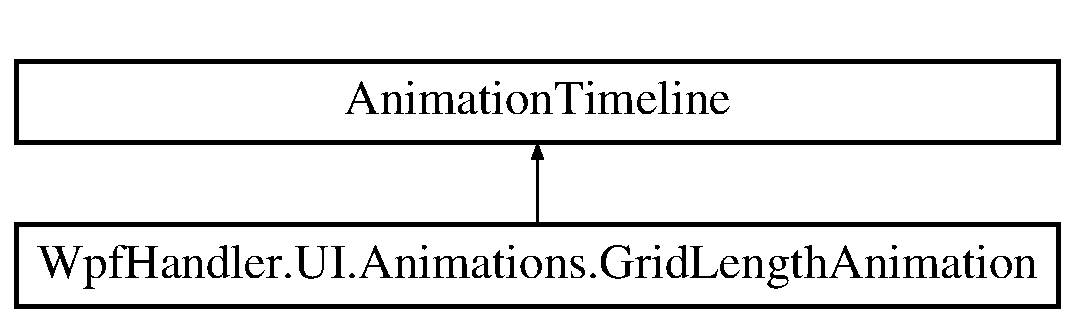
\includegraphics[height=2.000000cm]{de/d1a/class_wpf_handler_1_1_u_i_1_1_animations_1_1_grid_length_animation}
\end{center}
\end{figure}
\subsection*{Classes}
\begin{DoxyCompactItemize}
\item 
class \mbox{\hyperlink{class_wpf_handler_1_1_u_i_1_1_animations_1_1_grid_length_animation_1_1_expander_double_animation}{Expander\+Double\+Animation}}
\begin{DoxyCompactList}\small\item\em Animates a double value \end{DoxyCompactList}\end{DoxyCompactItemize}
\subsection*{Public Member Functions}
\begin{DoxyCompactItemize}
\item 
override object \mbox{\hyperlink{class_wpf_handler_1_1_u_i_1_1_animations_1_1_grid_length_animation_ae2f932054a13cdbe756f997ca4981708}{Get\+Current\+Value}} (object default\+Origin\+Value, object default\+Destination\+Value, Animation\+Clock animation\+Clock)
\begin{DoxyCompactList}\small\item\em Animates the grid let set \end{DoxyCompactList}\end{DoxyCompactItemize}
\subsection*{Static Public Member Functions}
\begin{DoxyCompactItemize}
\item 
static Storyboard \mbox{\hyperlink{class_wpf_handler_1_1_u_i_1_1_animations_1_1_grid_length_animation_a7ad925b0243e7b71b3aa51dcf5fd1bae}{Start\+Storyboard}} (Framework\+Element parent, Dependency\+Object control, Property\+Path property\+Path, Time\+Span duration, Fill\+Behavior fill\+Behavior, Grid\+Length from, Grid\+Length to, Action$<$ Storyboard $>$ init\+Handler)
\begin{DoxyCompactList}\small\item\em Creating story board with that animation. \end{DoxyCompactList}\end{DoxyCompactItemize}
\subsection*{Static Public Attributes}
\begin{DoxyCompactItemize}
\item 
static readonly Dependency\+Property \mbox{\hyperlink{class_wpf_handler_1_1_u_i_1_1_animations_1_1_grid_length_animation_a1f22e25ed15efee7758a5c1cdbe97965}{Reverse\+Value\+Property}}
\begin{DoxyCompactList}\small\item\em Dependency property. Sets the reverse value for the second animation \end{DoxyCompactList}\item 
static readonly Dependency\+Property \mbox{\hyperlink{class_wpf_handler_1_1_u_i_1_1_animations_1_1_grid_length_animation_a6950b177c05db4b6cab2705c1081c610}{From\+Property}}
\begin{DoxyCompactList}\small\item\em Dependency property for the From property \end{DoxyCompactList}\item 
static readonly Dependency\+Property \mbox{\hyperlink{class_wpf_handler_1_1_u_i_1_1_animations_1_1_grid_length_animation_ad46e81c2929885dacbff706b3c860146}{To\+Property}}
\begin{DoxyCompactList}\small\item\em Dependency property for the To property \end{DoxyCompactList}\end{DoxyCompactItemize}
\subsection*{Protected Member Functions}
\begin{DoxyCompactItemize}
\item 
override System.\+Windows.\+Freezable \mbox{\hyperlink{class_wpf_handler_1_1_u_i_1_1_animations_1_1_grid_length_animation_abf8dc83d562a5f43c9764c70d2d015f5}{Create\+Instance\+Core}} ()
\begin{DoxyCompactList}\small\item\em Creates an instance of the animation object \end{DoxyCompactList}\end{DoxyCompactItemize}
\subsection*{Properties}
\begin{DoxyCompactItemize}
\item 
bool \mbox{\hyperlink{class_wpf_handler_1_1_u_i_1_1_animations_1_1_grid_length_animation_a3884f38947db1a24ecc696b13a1e5ac4}{Is\+Completed}}\hspace{0.3cm}{\ttfamily  \mbox{[}get, set\mbox{]}}
\begin{DoxyCompactList}\small\item\em Marks the animation as completed \end{DoxyCompactList}\item 
double \mbox{\hyperlink{class_wpf_handler_1_1_u_i_1_1_animations_1_1_grid_length_animation_ab18d4bb2c37fd3d38cd285e12db18871}{Reverse\+Value}}\hspace{0.3cm}{\ttfamily  \mbox{[}get, set\mbox{]}}
\begin{DoxyCompactList}\small\item\em Sets the reverse value for the second animation \end{DoxyCompactList}\item 
override Type \mbox{\hyperlink{class_wpf_handler_1_1_u_i_1_1_animations_1_1_grid_length_animation_ac760bbe0c78eee7b3346f74f68024baa}{Target\+Property\+Type}}\hspace{0.3cm}{\ttfamily  \mbox{[}get\mbox{]}}
\begin{DoxyCompactList}\small\item\em Returns the type of object to animate \end{DoxyCompactList}\item 
Grid\+Length \mbox{\hyperlink{class_wpf_handler_1_1_u_i_1_1_animations_1_1_grid_length_animation_a6985f4dbd3e753ed873302a37ff542fe}{From}}\hspace{0.3cm}{\ttfamily  \mbox{[}get, set\mbox{]}}
\begin{DoxyCompactList}\small\item\em C\+LR Wrapper for the From depenendency property \end{DoxyCompactList}\item 
Grid\+Length \mbox{\hyperlink{class_wpf_handler_1_1_u_i_1_1_animations_1_1_grid_length_animation_a35b8e40718a9b06d82180d0e4aa9ffe0}{To}}\hspace{0.3cm}{\ttfamily  \mbox{[}get, set\mbox{]}}
\begin{DoxyCompactList}\small\item\em C\+LR Wrapper for the To property \end{DoxyCompactList}\end{DoxyCompactItemize}
\subsection*{Private Member Functions}
\begin{DoxyCompactItemize}
\item 
void \mbox{\hyperlink{class_wpf_handler_1_1_u_i_1_1_animations_1_1_grid_length_animation_ad162ed70827b35263f8e39939a0dcdcd}{Verify\+Animation\+Completed\+Status}} (Animation\+Clock clock)
\begin{DoxyCompactList}\small\item\em registers to the completed event of the animation clock \end{DoxyCompactList}\end{DoxyCompactItemize}
\subsection*{Private Attributes}
\begin{DoxyCompactItemize}
\item 
\mbox{\Hypertarget{class_wpf_handler_1_1_u_i_1_1_animations_1_1_grid_length_animation_a2a54b9ff4062d6c4ad47f28e137cfafe}\label{class_wpf_handler_1_1_u_i_1_1_animations_1_1_grid_length_animation_a2a54b9ff4062d6c4ad47f28e137cfafe}} 
bool {\bfseries is\+Completed}
\item 
\mbox{\Hypertarget{class_wpf_handler_1_1_u_i_1_1_animations_1_1_grid_length_animation_a2e79bc9b3aaa95f1f3d8e986b22d9540}\label{class_wpf_handler_1_1_u_i_1_1_animations_1_1_grid_length_animation_a2e79bc9b3aaa95f1f3d8e986b22d9540}} 
Animation\+Clock {\bfseries clock}
\end{DoxyCompactItemize}


\subsection{Detailed Description}
Animates a grid length value just like the Double\+Animation animates a double value 



\subsection{Member Function Documentation}
\mbox{\Hypertarget{class_wpf_handler_1_1_u_i_1_1_animations_1_1_grid_length_animation_abf8dc83d562a5f43c9764c70d2d015f5}\label{class_wpf_handler_1_1_u_i_1_1_animations_1_1_grid_length_animation_abf8dc83d562a5f43c9764c70d2d015f5}} 
\index{Wpf\+Handler\+::\+U\+I\+::\+Animations\+::\+Grid\+Length\+Animation@{Wpf\+Handler\+::\+U\+I\+::\+Animations\+::\+Grid\+Length\+Animation}!Create\+Instance\+Core@{Create\+Instance\+Core}}
\index{Create\+Instance\+Core@{Create\+Instance\+Core}!Wpf\+Handler\+::\+U\+I\+::\+Animations\+::\+Grid\+Length\+Animation@{Wpf\+Handler\+::\+U\+I\+::\+Animations\+::\+Grid\+Length\+Animation}}
\subsubsection{\texorpdfstring{Create\+Instance\+Core()}{CreateInstanceCore()}}
{\footnotesize\ttfamily override System.\+Windows.\+Freezable Wpf\+Handler.\+U\+I.\+Animations.\+Grid\+Length\+Animation.\+Create\+Instance\+Core (\begin{DoxyParamCaption}{ }\end{DoxyParamCaption})\hspace{0.3cm}{\ttfamily [protected]}}



Creates an instance of the animation object 

\begin{DoxyReturn}{Returns}
Returns the instance of the \mbox{\hyperlink{class_wpf_handler_1_1_u_i_1_1_animations_1_1_grid_length_animation}{Grid\+Length\+Animation}}
\end{DoxyReturn}
\mbox{\Hypertarget{class_wpf_handler_1_1_u_i_1_1_animations_1_1_grid_length_animation_ae2f932054a13cdbe756f997ca4981708}\label{class_wpf_handler_1_1_u_i_1_1_animations_1_1_grid_length_animation_ae2f932054a13cdbe756f997ca4981708}} 
\index{Wpf\+Handler\+::\+U\+I\+::\+Animations\+::\+Grid\+Length\+Animation@{Wpf\+Handler\+::\+U\+I\+::\+Animations\+::\+Grid\+Length\+Animation}!Get\+Current\+Value@{Get\+Current\+Value}}
\index{Get\+Current\+Value@{Get\+Current\+Value}!Wpf\+Handler\+::\+U\+I\+::\+Animations\+::\+Grid\+Length\+Animation@{Wpf\+Handler\+::\+U\+I\+::\+Animations\+::\+Grid\+Length\+Animation}}
\subsubsection{\texorpdfstring{Get\+Current\+Value()}{GetCurrentValue()}}
{\footnotesize\ttfamily override object Wpf\+Handler.\+U\+I.\+Animations.\+Grid\+Length\+Animation.\+Get\+Current\+Value (\begin{DoxyParamCaption}\item[{object}]{default\+Origin\+Value,  }\item[{object}]{default\+Destination\+Value,  }\item[{Animation\+Clock}]{animation\+Clock }\end{DoxyParamCaption})}



Animates the grid let set 


\begin{DoxyParams}{Parameters}
{\em default\+Origin\+Value} & The original value to animate\\
\hline
{\em default\+Destination\+Value} & The final value\\
\hline
{\em animation\+Clock} & The animation clock (timer)\\
\hline
\end{DoxyParams}
\begin{DoxyReturn}{Returns}
Returns the new grid length to set
\end{DoxyReturn}
\mbox{\Hypertarget{class_wpf_handler_1_1_u_i_1_1_animations_1_1_grid_length_animation_a7ad925b0243e7b71b3aa51dcf5fd1bae}\label{class_wpf_handler_1_1_u_i_1_1_animations_1_1_grid_length_animation_a7ad925b0243e7b71b3aa51dcf5fd1bae}} 
\index{Wpf\+Handler\+::\+U\+I\+::\+Animations\+::\+Grid\+Length\+Animation@{Wpf\+Handler\+::\+U\+I\+::\+Animations\+::\+Grid\+Length\+Animation}!Start\+Storyboard@{Start\+Storyboard}}
\index{Start\+Storyboard@{Start\+Storyboard}!Wpf\+Handler\+::\+U\+I\+::\+Animations\+::\+Grid\+Length\+Animation@{Wpf\+Handler\+::\+U\+I\+::\+Animations\+::\+Grid\+Length\+Animation}}
\subsubsection{\texorpdfstring{Start\+Storyboard()}{StartStoryboard()}}
{\footnotesize\ttfamily static Storyboard Wpf\+Handler.\+U\+I.\+Animations.\+Grid\+Length\+Animation.\+Start\+Storyboard (\begin{DoxyParamCaption}\item[{Framework\+Element}]{parent,  }\item[{Dependency\+Object}]{control,  }\item[{Property\+Path}]{property\+Path,  }\item[{Time\+Span}]{duration,  }\item[{Fill\+Behavior}]{fill\+Behavior,  }\item[{Grid\+Length}]{from,  }\item[{Grid\+Length}]{to,  }\item[{Action$<$ Storyboard $>$}]{init\+Handler }\end{DoxyParamCaption})\hspace{0.3cm}{\ttfamily [static]}}



Creating story board with that animation. 


\begin{DoxyParams}{Parameters}
{\em parent} & \\
\hline
{\em control} & \\
\hline
{\em property\+Path} & \\
\hline
{\em duration} & \\
\hline
{\em fill\+Behavior} & \\
\hline
{\em from} & \\
\hline
{\em to} & \\
\hline
{\em init\+Handler} & \\
\hline
\end{DoxyParams}
\begin{DoxyReturn}{Returns}

\end{DoxyReturn}
\mbox{\Hypertarget{class_wpf_handler_1_1_u_i_1_1_animations_1_1_grid_length_animation_ad162ed70827b35263f8e39939a0dcdcd}\label{class_wpf_handler_1_1_u_i_1_1_animations_1_1_grid_length_animation_ad162ed70827b35263f8e39939a0dcdcd}} 
\index{Wpf\+Handler\+::\+U\+I\+::\+Animations\+::\+Grid\+Length\+Animation@{Wpf\+Handler\+::\+U\+I\+::\+Animations\+::\+Grid\+Length\+Animation}!Verify\+Animation\+Completed\+Status@{Verify\+Animation\+Completed\+Status}}
\index{Verify\+Animation\+Completed\+Status@{Verify\+Animation\+Completed\+Status}!Wpf\+Handler\+::\+U\+I\+::\+Animations\+::\+Grid\+Length\+Animation@{Wpf\+Handler\+::\+U\+I\+::\+Animations\+::\+Grid\+Length\+Animation}}
\subsubsection{\texorpdfstring{Verify\+Animation\+Completed\+Status()}{VerifyAnimationCompletedStatus()}}
{\footnotesize\ttfamily void Wpf\+Handler.\+U\+I.\+Animations.\+Grid\+Length\+Animation.\+Verify\+Animation\+Completed\+Status (\begin{DoxyParamCaption}\item[{Animation\+Clock}]{clock }\end{DoxyParamCaption})\hspace{0.3cm}{\ttfamily [private]}}



registers to the completed event of the animation clock 


\begin{DoxyParams}{Parameters}
{\em clock} & the animation clock to notify completion status\\
\hline
\end{DoxyParams}


\subsection{Member Data Documentation}
\mbox{\Hypertarget{class_wpf_handler_1_1_u_i_1_1_animations_1_1_grid_length_animation_a6950b177c05db4b6cab2705c1081c610}\label{class_wpf_handler_1_1_u_i_1_1_animations_1_1_grid_length_animation_a6950b177c05db4b6cab2705c1081c610}} 
\index{Wpf\+Handler\+::\+U\+I\+::\+Animations\+::\+Grid\+Length\+Animation@{Wpf\+Handler\+::\+U\+I\+::\+Animations\+::\+Grid\+Length\+Animation}!From\+Property@{From\+Property}}
\index{From\+Property@{From\+Property}!Wpf\+Handler\+::\+U\+I\+::\+Animations\+::\+Grid\+Length\+Animation@{Wpf\+Handler\+::\+U\+I\+::\+Animations\+::\+Grid\+Length\+Animation}}
\subsubsection{\texorpdfstring{From\+Property}{FromProperty}}
{\footnotesize\ttfamily readonly Dependency\+Property Wpf\+Handler.\+U\+I.\+Animations.\+Grid\+Length\+Animation.\+From\+Property\hspace{0.3cm}{\ttfamily [static]}}

{\bfseries Initial value\+:}
\begin{DoxyCode}
= DependencyProperty.Register(\textcolor{stringliteral}{"From"}, typeof(GridLength),
                typeof(GridLengthAnimation))
\end{DoxyCode}


Dependency property for the From property 

\mbox{\Hypertarget{class_wpf_handler_1_1_u_i_1_1_animations_1_1_grid_length_animation_a1f22e25ed15efee7758a5c1cdbe97965}\label{class_wpf_handler_1_1_u_i_1_1_animations_1_1_grid_length_animation_a1f22e25ed15efee7758a5c1cdbe97965}} 
\index{Wpf\+Handler\+::\+U\+I\+::\+Animations\+::\+Grid\+Length\+Animation@{Wpf\+Handler\+::\+U\+I\+::\+Animations\+::\+Grid\+Length\+Animation}!Reverse\+Value\+Property@{Reverse\+Value\+Property}}
\index{Reverse\+Value\+Property@{Reverse\+Value\+Property}!Wpf\+Handler\+::\+U\+I\+::\+Animations\+::\+Grid\+Length\+Animation@{Wpf\+Handler\+::\+U\+I\+::\+Animations\+::\+Grid\+Length\+Animation}}
\subsubsection{\texorpdfstring{Reverse\+Value\+Property}{ReverseValueProperty}}
{\footnotesize\ttfamily readonly Dependency\+Property Wpf\+Handler.\+U\+I.\+Animations.\+Grid\+Length\+Animation.\+Reverse\+Value\+Property\hspace{0.3cm}{\ttfamily [static]}}

{\bfseries Initial value\+:}
\begin{DoxyCode}
=
            DependencyProperty.Register(\textcolor{stringliteral}{"ReverseValue"}, typeof(\textcolor{keywordtype}{double}), typeof(GridLengthAnimation), \textcolor{keyword}{new} 
      UIPropertyMetadata(0.0))
\end{DoxyCode}


Dependency property. Sets the reverse value for the second animation 

\mbox{\Hypertarget{class_wpf_handler_1_1_u_i_1_1_animations_1_1_grid_length_animation_ad46e81c2929885dacbff706b3c860146}\label{class_wpf_handler_1_1_u_i_1_1_animations_1_1_grid_length_animation_ad46e81c2929885dacbff706b3c860146}} 
\index{Wpf\+Handler\+::\+U\+I\+::\+Animations\+::\+Grid\+Length\+Animation@{Wpf\+Handler\+::\+U\+I\+::\+Animations\+::\+Grid\+Length\+Animation}!To\+Property@{To\+Property}}
\index{To\+Property@{To\+Property}!Wpf\+Handler\+::\+U\+I\+::\+Animations\+::\+Grid\+Length\+Animation@{Wpf\+Handler\+::\+U\+I\+::\+Animations\+::\+Grid\+Length\+Animation}}
\subsubsection{\texorpdfstring{To\+Property}{ToProperty}}
{\footnotesize\ttfamily readonly Dependency\+Property Wpf\+Handler.\+U\+I.\+Animations.\+Grid\+Length\+Animation.\+To\+Property\hspace{0.3cm}{\ttfamily [static]}}

{\bfseries Initial value\+:}
\begin{DoxyCode}
= DependencyProperty.Register(\textcolor{stringliteral}{"To"}, typeof(GridLength),
                typeof(GridLengthAnimation))
\end{DoxyCode}


Dependency property for the To property 



\subsection{Property Documentation}
\mbox{\Hypertarget{class_wpf_handler_1_1_u_i_1_1_animations_1_1_grid_length_animation_a6985f4dbd3e753ed873302a37ff542fe}\label{class_wpf_handler_1_1_u_i_1_1_animations_1_1_grid_length_animation_a6985f4dbd3e753ed873302a37ff542fe}} 
\index{Wpf\+Handler\+::\+U\+I\+::\+Animations\+::\+Grid\+Length\+Animation@{Wpf\+Handler\+::\+U\+I\+::\+Animations\+::\+Grid\+Length\+Animation}!From@{From}}
\index{From@{From}!Wpf\+Handler\+::\+U\+I\+::\+Animations\+::\+Grid\+Length\+Animation@{Wpf\+Handler\+::\+U\+I\+::\+Animations\+::\+Grid\+Length\+Animation}}
\subsubsection{\texorpdfstring{From}{From}}
{\footnotesize\ttfamily Grid\+Length Wpf\+Handler.\+U\+I.\+Animations.\+Grid\+Length\+Animation.\+From\hspace{0.3cm}{\ttfamily [get]}, {\ttfamily [set]}}



C\+LR Wrapper for the From depenendency property 

\mbox{\Hypertarget{class_wpf_handler_1_1_u_i_1_1_animations_1_1_grid_length_animation_a3884f38947db1a24ecc696b13a1e5ac4}\label{class_wpf_handler_1_1_u_i_1_1_animations_1_1_grid_length_animation_a3884f38947db1a24ecc696b13a1e5ac4}} 
\index{Wpf\+Handler\+::\+U\+I\+::\+Animations\+::\+Grid\+Length\+Animation@{Wpf\+Handler\+::\+U\+I\+::\+Animations\+::\+Grid\+Length\+Animation}!Is\+Completed@{Is\+Completed}}
\index{Is\+Completed@{Is\+Completed}!Wpf\+Handler\+::\+U\+I\+::\+Animations\+::\+Grid\+Length\+Animation@{Wpf\+Handler\+::\+U\+I\+::\+Animations\+::\+Grid\+Length\+Animation}}
\subsubsection{\texorpdfstring{Is\+Completed}{IsCompleted}}
{\footnotesize\ttfamily bool Wpf\+Handler.\+U\+I.\+Animations.\+Grid\+Length\+Animation.\+Is\+Completed\hspace{0.3cm}{\ttfamily [get]}, {\ttfamily [set]}}



Marks the animation as completed 

\mbox{\Hypertarget{class_wpf_handler_1_1_u_i_1_1_animations_1_1_grid_length_animation_ab18d4bb2c37fd3d38cd285e12db18871}\label{class_wpf_handler_1_1_u_i_1_1_animations_1_1_grid_length_animation_ab18d4bb2c37fd3d38cd285e12db18871}} 
\index{Wpf\+Handler\+::\+U\+I\+::\+Animations\+::\+Grid\+Length\+Animation@{Wpf\+Handler\+::\+U\+I\+::\+Animations\+::\+Grid\+Length\+Animation}!Reverse\+Value@{Reverse\+Value}}
\index{Reverse\+Value@{Reverse\+Value}!Wpf\+Handler\+::\+U\+I\+::\+Animations\+::\+Grid\+Length\+Animation@{Wpf\+Handler\+::\+U\+I\+::\+Animations\+::\+Grid\+Length\+Animation}}
\subsubsection{\texorpdfstring{Reverse\+Value}{ReverseValue}}
{\footnotesize\ttfamily double Wpf\+Handler.\+U\+I.\+Animations.\+Grid\+Length\+Animation.\+Reverse\+Value\hspace{0.3cm}{\ttfamily [get]}, {\ttfamily [set]}}



Sets the reverse value for the second animation 

\mbox{\Hypertarget{class_wpf_handler_1_1_u_i_1_1_animations_1_1_grid_length_animation_ac760bbe0c78eee7b3346f74f68024baa}\label{class_wpf_handler_1_1_u_i_1_1_animations_1_1_grid_length_animation_ac760bbe0c78eee7b3346f74f68024baa}} 
\index{Wpf\+Handler\+::\+U\+I\+::\+Animations\+::\+Grid\+Length\+Animation@{Wpf\+Handler\+::\+U\+I\+::\+Animations\+::\+Grid\+Length\+Animation}!Target\+Property\+Type@{Target\+Property\+Type}}
\index{Target\+Property\+Type@{Target\+Property\+Type}!Wpf\+Handler\+::\+U\+I\+::\+Animations\+::\+Grid\+Length\+Animation@{Wpf\+Handler\+::\+U\+I\+::\+Animations\+::\+Grid\+Length\+Animation}}
\subsubsection{\texorpdfstring{Target\+Property\+Type}{TargetPropertyType}}
{\footnotesize\ttfamily override Type Wpf\+Handler.\+U\+I.\+Animations.\+Grid\+Length\+Animation.\+Target\+Property\+Type\hspace{0.3cm}{\ttfamily [get]}}



Returns the type of object to animate 

\mbox{\Hypertarget{class_wpf_handler_1_1_u_i_1_1_animations_1_1_grid_length_animation_a35b8e40718a9b06d82180d0e4aa9ffe0}\label{class_wpf_handler_1_1_u_i_1_1_animations_1_1_grid_length_animation_a35b8e40718a9b06d82180d0e4aa9ffe0}} 
\index{Wpf\+Handler\+::\+U\+I\+::\+Animations\+::\+Grid\+Length\+Animation@{Wpf\+Handler\+::\+U\+I\+::\+Animations\+::\+Grid\+Length\+Animation}!To@{To}}
\index{To@{To}!Wpf\+Handler\+::\+U\+I\+::\+Animations\+::\+Grid\+Length\+Animation@{Wpf\+Handler\+::\+U\+I\+::\+Animations\+::\+Grid\+Length\+Animation}}
\subsubsection{\texorpdfstring{To}{To}}
{\footnotesize\ttfamily Grid\+Length Wpf\+Handler.\+U\+I.\+Animations.\+Grid\+Length\+Animation.\+To\hspace{0.3cm}{\ttfamily [get]}, {\ttfamily [set]}}



C\+LR Wrapper for the To property 



The documentation for this class was generated from the following file\+:\begin{DoxyCompactItemize}
\item 
D\+:/\+Work/\+Git\+Hub/wpf-\/handler/\+Wpf\+Handler/\+U\+I/\+Animations/Grid\+Length\+Animation.\+cs\end{DoxyCompactItemize}

\hypertarget{class_wpf_handler_1_1_u_i_1_1_g_u_i_content}{}\section{Wpf\+Handler.\+U\+I.\+G\+U\+I\+Content Class Reference}
\label{class_wpf_handler_1_1_u_i_1_1_g_u_i_content}\index{Wpf\+Handler.\+U\+I.\+G\+U\+I\+Content@{Wpf\+Handler.\+U\+I.\+G\+U\+I\+Content}}


Define content of G\+UI lement.  


Inheritance diagram for Wpf\+Handler.\+U\+I.\+G\+U\+I\+Content\+:\begin{figure}[H]
\begin{center}
\leavevmode
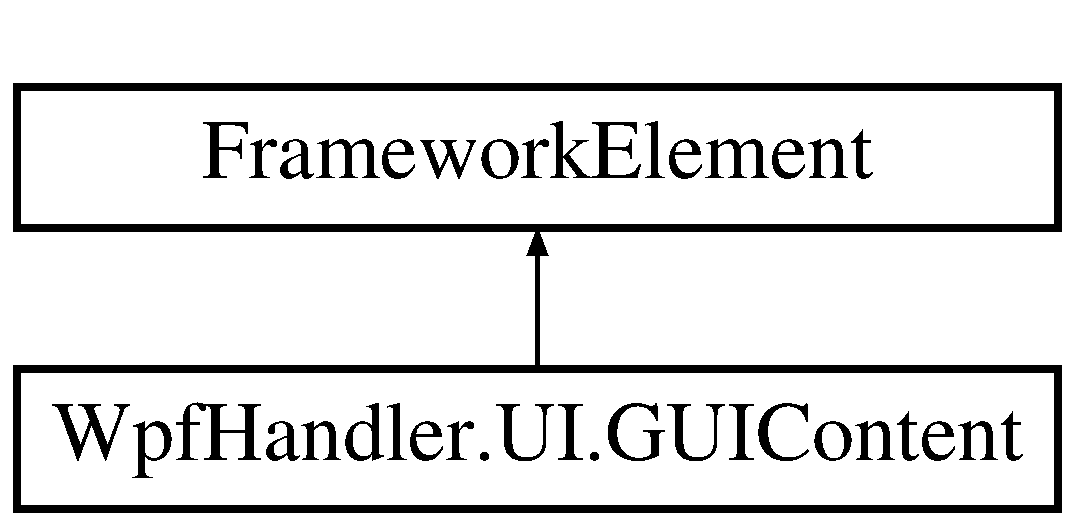
\includegraphics[height=2.000000cm]{db/dd5/class_wpf_handler_1_1_u_i_1_1_g_u_i_content}
\end{center}
\end{figure}
\subsection*{Public Member Functions}
\begin{DoxyCompactItemize}
\item 
\mbox{\hyperlink{class_wpf_handler_1_1_u_i_1_1_g_u_i_content_a94df176704a9da39956a31d4cc1f3aeb}{G\+U\+I\+Content}} ()
\begin{DoxyCompactList}\small\item\em Default constructor. \end{DoxyCompactList}\item 
\mbox{\hyperlink{class_wpf_handler_1_1_u_i_1_1_g_u_i_content_a4608943cf14878430faed858fb93b6fa}{G\+U\+I\+Content}} (string title)
\begin{DoxyCompactList}\small\item\em Constructor that allow to set title. \end{DoxyCompactList}\item 
\mbox{\hyperlink{class_wpf_handler_1_1_u_i_1_1_g_u_i_content_a1b6b06ba3dceb601146432dc2366240f}{G\+U\+I\+Content}} (string title, string description)
\begin{DoxyCompactList}\small\item\em Constructor that allow to set title. \end{DoxyCompactList}\item 
\mbox{\hyperlink{class_wpf_handler_1_1_u_i_1_1_g_u_i_content_a04d4c3d50ac71b80f193a3f8539a70ac}{G\+U\+I\+Content}} (string default\+Title, string default\+Description, string decription\+Localization\+Resourse\+Key)
\begin{DoxyCompactList}\small\item\em Initialize all allowed fields. \end{DoxyCompactList}\item 
\mbox{\hyperlink{class_wpf_handler_1_1_u_i_1_1_g_u_i_content_a20eef2a05ca7432cdb0b56731f1ec47b}{G\+U\+I\+Content}} (string default\+Title, string default\+Description, string title\+Localization\+Resourse\+Key, string decription\+Localization\+Resourse\+Key)
\begin{DoxyCompactList}\small\item\em Initialize all allowed fields. \end{DoxyCompactList}\item 
string \mbox{\hyperlink{class_wpf_handler_1_1_u_i_1_1_g_u_i_content_a06b4859ce09ed1dc91545154cdb9d5c3}{Get\+Title}} ()
\begin{DoxyCompactList}\small\item\em Define relevant title for certain member. \end{DoxyCompactList}\item 
string \mbox{\hyperlink{class_wpf_handler_1_1_u_i_1_1_g_u_i_content_a36c48561703ca7b73f21187ee9ff08bb}{Get\+Title}} (Member\+Info member)
\begin{DoxyCompactList}\small\item\em Define relevant title for certain member. \end{DoxyCompactList}\item 
string \mbox{\hyperlink{class_wpf_handler_1_1_u_i_1_1_g_u_i_content_a98ca8cae768fad4160df1aba48d6f7f6}{Get\+Description}} ()
\begin{DoxyCompactList}\small\item\em Define relevant description for certain member. \end{DoxyCompactList}\item 
string \mbox{\hyperlink{class_wpf_handler_1_1_u_i_1_1_g_u_i_content_ad37327acd55ad09e036f284970d1e022}{Format}} (string member\+Name)
\begin{DoxyCompactList}\small\item\em Format member name to user reandly veiw. \end{DoxyCompactList}\item 
void \mbox{\hyperlink{class_wpf_handler_1_1_u_i_1_1_g_u_i_content_ae691340b5a25a5497d9f64d4b0adddd6}{Clear}} ()
\begin{DoxyCompactList}\small\item\em Clearing current data. To allow update. \end{DoxyCompactList}\item 
override string \mbox{\hyperlink{class_wpf_handler_1_1_u_i_1_1_g_u_i_content_ae38dd5281ee8568b040af4c1d14322c4}{To\+String}} ()
\begin{DoxyCompactList}\small\item\em Return the G\+UI content in the string format. \end{DoxyCompactList}\end{DoxyCompactItemize}
\subsection*{Static Public Member Functions}
\begin{DoxyCompactItemize}
\item 
static implicit \mbox{\hyperlink{class_wpf_handler_1_1_u_i_1_1_g_u_i_content_a0a59156d78345550a413d155791e1137}{operator string}} (\mbox{\hyperlink{class_wpf_handler_1_1_u_i_1_1_g_u_i_content}{G\+U\+I\+Content}} content)
\begin{DoxyCompactList}\small\item\em Converting the \mbox{\hyperlink{class_wpf_handler_1_1_u_i_1_1_g_u_i_content}{G\+U\+I\+Content}} to he string format. \end{DoxyCompactList}\end{DoxyCompactItemize}
\subsection*{Properties}
\begin{DoxyCompactItemize}
\item 
static \mbox{\hyperlink{class_wpf_handler_1_1_u_i_1_1_g_u_i_content}{G\+U\+I\+Content}} \mbox{\hyperlink{class_wpf_handler_1_1_u_i_1_1_g_u_i_content_a9d8259c5a572b9ab33faab8166fc6053}{None}}\hspace{0.3cm}{\ttfamily  \mbox{[}get\mbox{]}}
\begin{DoxyCompactList}\small\item\em Empty content. Can\textquotesingle{}t change none state after instiniation. \end{DoxyCompactList}\item 
string \mbox{\hyperlink{class_wpf_handler_1_1_u_i_1_1_g_u_i_content_afa422133cdb4b7e81ab4041e3bcb93ca}{Default\+Title}}\hspace{0.3cm}{\ttfamily  \mbox{[}get, set\mbox{]}}
\begin{DoxyCompactList}\small\item\em Title that would be used by default in case if dynamic dictionry not found. in case if null then would be automaticly generated from the name of the binded member. \end{DoxyCompactList}\item 
string \mbox{\hyperlink{class_wpf_handler_1_1_u_i_1_1_g_u_i_content_afc956b837fa7495d33e25aba7995297b}{Default\+Description}}\hspace{0.3cm}{\ttfamily  \mbox{[}get, set\mbox{]}}
\begin{DoxyCompactList}\small\item\em Description that would be used by default in case if dynamic dictionry not found. \end{DoxyCompactList}\item 
string \mbox{\hyperlink{class_wpf_handler_1_1_u_i_1_1_g_u_i_content_a3d8843f4aaceba1bb1174f33c925bab2}{Title\+Localization\+Resourse\+Key}}\hspace{0.3cm}{\ttfamily  \mbox{[}get, set\mbox{]}}
\begin{DoxyCompactList}\small\item\em Key of resource from dynamic dictionary that would be used for loading of localized title. \end{DoxyCompactList}\item 
string \mbox{\hyperlink{class_wpf_handler_1_1_u_i_1_1_g_u_i_content_a03f871ffe5fe0858b5be321e356393ee}{Decription\+Localization\+Resourse\+Key}}\hspace{0.3cm}{\ttfamily  \mbox{[}get, set\mbox{]}}
\begin{DoxyCompactList}\small\item\em Key of resource from dynamic dictionary that would be used for loading of localized description. \end{DoxyCompactList}\item 
bool \mbox{\hyperlink{class_wpf_handler_1_1_u_i_1_1_g_u_i_content_ab8044a6651911a3b52f47b4cc6c485cd}{Is\+None}}\hspace{0.3cm}{\ttfamily  \mbox{[}get\mbox{]}}
\begin{DoxyCompactList}\small\item\em Is that conent is defult none. \end{DoxyCompactList}\end{DoxyCompactItemize}
\subsection*{Events}
\begin{DoxyCompactItemize}
\item 
Action$<$ \mbox{\hyperlink{class_wpf_handler_1_1_u_i_1_1_g_u_i_content}{G\+U\+I\+Content}} $>$ \mbox{\hyperlink{class_wpf_handler_1_1_u_i_1_1_g_u_i_content_a165b9cf266e359c62f576b07ee9865ad}{Content\+Updated}}
\begin{DoxyCompactList}\small\item\em Event that will occure when content properties will updated. \end{DoxyCompactList}\end{DoxyCompactItemize}
\subsection*{Private Member Functions}
\begin{DoxyCompactItemize}
\item 
\mbox{\hyperlink{class_wpf_handler_1_1_u_i_1_1_g_u_i_content_a6bd38c606c795603ab17e2d6acfec72f}{$\sim$\+G\+U\+I\+Content}} ()
\begin{DoxyCompactList}\small\item\em Resliasing unmanged memory. \end{DoxyCompactList}\item 
void \mbox{\hyperlink{class_wpf_handler_1_1_u_i_1_1_g_u_i_content_a05536bbfc1d91f3c2db9bea9ae2dc468}{A\+P\+I\+\_\+\+Languages\+Dictionaries\+Updated}} ()
\begin{DoxyCompactList}\small\item\em W\+Ill occure when new pool of language dictionaries will loaded. Drop current value to allow reloading. \end{DoxyCompactList}\end{DoxyCompactItemize}
\subsection*{Private Attributes}
\begin{DoxyCompactItemize}
\item 
string \mbox{\hyperlink{class_wpf_handler_1_1_u_i_1_1_g_u_i_content_af02b5c5e573d3bb9a92dfd9063690d1d}{\+\_\+\+Title}}
\begin{DoxyCompactList}\small\item\em Bufer that contains last defined title. \end{DoxyCompactList}\item 
string \mbox{\hyperlink{class_wpf_handler_1_1_u_i_1_1_g_u_i_content_a2589ade8a7b670ed7091b7c658863bb7}{\+\_\+\+Description}}
\begin{DoxyCompactList}\small\item\em Bufer that contains last defined description. \end{DoxyCompactList}\item 
bool \mbox{\hyperlink{class_wpf_handler_1_1_u_i_1_1_g_u_i_content_afffba81fad8d7a802ec0f55a6c8b9da7}{\+\_\+is\+None}} = false
\begin{DoxyCompactList}\small\item\em is that content is none. \end{DoxyCompactList}\item 
string \mbox{\hyperlink{class_wpf_handler_1_1_u_i_1_1_g_u_i_content_a7bfdcdd062eaf3f8cadcdb34eed52d2f}{\+\_\+\+Default\+Title}} = null
\begin{DoxyCompactList}\small\item\em Title that would be used by default in case if dynamic dictionry not found. in case if null then would be automaticly generated from the name of the binded member. \end{DoxyCompactList}\item 
string \mbox{\hyperlink{class_wpf_handler_1_1_u_i_1_1_g_u_i_content_a7d0ce7f98f08a7e1373eb150231d0c56}{\+\_\+\+Default\+Description}} = null
\begin{DoxyCompactList}\small\item\em Description that would be used by default in case if dynamic dictionry not found. \end{DoxyCompactList}\item 
string \mbox{\hyperlink{class_wpf_handler_1_1_u_i_1_1_g_u_i_content_ac878075c0d59c6ce0c7b54a82b5843c8}{\+\_\+\+Title\+Localization\+Resourse\+Key}} = null
\begin{DoxyCompactList}\small\item\em Key of resource from dynamic dictionary that would be used for loading of localized title. \end{DoxyCompactList}\item 
string \mbox{\hyperlink{class_wpf_handler_1_1_u_i_1_1_g_u_i_content_a067181a637a28c683c1a24ed06e577ae}{\+\_\+\+Decription\+Localization\+Resourse\+Key}} = null
\begin{DoxyCompactList}\small\item\em Key of resource from dynamic dictionary that would be used for loading of localized description. \end{DoxyCompactList}\end{DoxyCompactItemize}


\subsection{Detailed Description}
Define content of G\+UI lement. 



\subsection{Constructor \& Destructor Documentation}
\mbox{\Hypertarget{class_wpf_handler_1_1_u_i_1_1_g_u_i_content_a94df176704a9da39956a31d4cc1f3aeb}\label{class_wpf_handler_1_1_u_i_1_1_g_u_i_content_a94df176704a9da39956a31d4cc1f3aeb}} 
\index{Wpf\+Handler\+::\+U\+I\+::\+G\+U\+I\+Content@{Wpf\+Handler\+::\+U\+I\+::\+G\+U\+I\+Content}!G\+U\+I\+Content@{G\+U\+I\+Content}}
\index{G\+U\+I\+Content@{G\+U\+I\+Content}!Wpf\+Handler\+::\+U\+I\+::\+G\+U\+I\+Content@{Wpf\+Handler\+::\+U\+I\+::\+G\+U\+I\+Content}}
\subsubsection{\texorpdfstring{G\+U\+I\+Content()}{GUIContent()}\hspace{0.1cm}{\footnotesize\ttfamily [1/5]}}
{\footnotesize\ttfamily Wpf\+Handler.\+U\+I.\+G\+U\+I\+Content.\+G\+U\+I\+Content (\begin{DoxyParamCaption}{ }\end{DoxyParamCaption})}



Default constructor. 

\mbox{\Hypertarget{class_wpf_handler_1_1_u_i_1_1_g_u_i_content_a4608943cf14878430faed858fb93b6fa}\label{class_wpf_handler_1_1_u_i_1_1_g_u_i_content_a4608943cf14878430faed858fb93b6fa}} 
\index{Wpf\+Handler\+::\+U\+I\+::\+G\+U\+I\+Content@{Wpf\+Handler\+::\+U\+I\+::\+G\+U\+I\+Content}!G\+U\+I\+Content@{G\+U\+I\+Content}}
\index{G\+U\+I\+Content@{G\+U\+I\+Content}!Wpf\+Handler\+::\+U\+I\+::\+G\+U\+I\+Content@{Wpf\+Handler\+::\+U\+I\+::\+G\+U\+I\+Content}}
\subsubsection{\texorpdfstring{G\+U\+I\+Content()}{GUIContent()}\hspace{0.1cm}{\footnotesize\ttfamily [2/5]}}
{\footnotesize\ttfamily Wpf\+Handler.\+U\+I.\+G\+U\+I\+Content.\+G\+U\+I\+Content (\begin{DoxyParamCaption}\item[{string}]{title }\end{DoxyParamCaption})}



Constructor that allow to set title. 


\begin{DoxyParams}{Parameters}
{\em title} & Title of the element.\\
\hline
\end{DoxyParams}
\mbox{\Hypertarget{class_wpf_handler_1_1_u_i_1_1_g_u_i_content_a1b6b06ba3dceb601146432dc2366240f}\label{class_wpf_handler_1_1_u_i_1_1_g_u_i_content_a1b6b06ba3dceb601146432dc2366240f}} 
\index{Wpf\+Handler\+::\+U\+I\+::\+G\+U\+I\+Content@{Wpf\+Handler\+::\+U\+I\+::\+G\+U\+I\+Content}!G\+U\+I\+Content@{G\+U\+I\+Content}}
\index{G\+U\+I\+Content@{G\+U\+I\+Content}!Wpf\+Handler\+::\+U\+I\+::\+G\+U\+I\+Content@{Wpf\+Handler\+::\+U\+I\+::\+G\+U\+I\+Content}}
\subsubsection{\texorpdfstring{G\+U\+I\+Content()}{GUIContent()}\hspace{0.1cm}{\footnotesize\ttfamily [3/5]}}
{\footnotesize\ttfamily Wpf\+Handler.\+U\+I.\+G\+U\+I\+Content.\+G\+U\+I\+Content (\begin{DoxyParamCaption}\item[{string}]{title,  }\item[{string}]{description }\end{DoxyParamCaption})}



Constructor that allow to set title. 


\begin{DoxyParams}{Parameters}
{\em title} & Title of that element.\\
\hline
{\em description} & Description of that element.\\
\hline
\end{DoxyParams}
\mbox{\Hypertarget{class_wpf_handler_1_1_u_i_1_1_g_u_i_content_a04d4c3d50ac71b80f193a3f8539a70ac}\label{class_wpf_handler_1_1_u_i_1_1_g_u_i_content_a04d4c3d50ac71b80f193a3f8539a70ac}} 
\index{Wpf\+Handler\+::\+U\+I\+::\+G\+U\+I\+Content@{Wpf\+Handler\+::\+U\+I\+::\+G\+U\+I\+Content}!G\+U\+I\+Content@{G\+U\+I\+Content}}
\index{G\+U\+I\+Content@{G\+U\+I\+Content}!Wpf\+Handler\+::\+U\+I\+::\+G\+U\+I\+Content@{Wpf\+Handler\+::\+U\+I\+::\+G\+U\+I\+Content}}
\subsubsection{\texorpdfstring{G\+U\+I\+Content()}{GUIContent()}\hspace{0.1cm}{\footnotesize\ttfamily [4/5]}}
{\footnotesize\ttfamily Wpf\+Handler.\+U\+I.\+G\+U\+I\+Content.\+G\+U\+I\+Content (\begin{DoxyParamCaption}\item[{string}]{default\+Title,  }\item[{string}]{default\+Description,  }\item[{string}]{decription\+Localization\+Resourse\+Key }\end{DoxyParamCaption})}



Initialize all allowed fields. 


\begin{DoxyParams}{Parameters}
{\em default\+Title} & Title that would be used by default if localization dictionary not found.\\
\hline
{\em default\+Description} & Default description if localization dictionary not found.\\
\hline
{\em decription\+Localization\+Resourse\+Key} & Key of description content in localized dynamic dictionary.\\
\hline
\end{DoxyParams}
\mbox{\Hypertarget{class_wpf_handler_1_1_u_i_1_1_g_u_i_content_a20eef2a05ca7432cdb0b56731f1ec47b}\label{class_wpf_handler_1_1_u_i_1_1_g_u_i_content_a20eef2a05ca7432cdb0b56731f1ec47b}} 
\index{Wpf\+Handler\+::\+U\+I\+::\+G\+U\+I\+Content@{Wpf\+Handler\+::\+U\+I\+::\+G\+U\+I\+Content}!G\+U\+I\+Content@{G\+U\+I\+Content}}
\index{G\+U\+I\+Content@{G\+U\+I\+Content}!Wpf\+Handler\+::\+U\+I\+::\+G\+U\+I\+Content@{Wpf\+Handler\+::\+U\+I\+::\+G\+U\+I\+Content}}
\subsubsection{\texorpdfstring{G\+U\+I\+Content()}{GUIContent()}\hspace{0.1cm}{\footnotesize\ttfamily [5/5]}}
{\footnotesize\ttfamily Wpf\+Handler.\+U\+I.\+G\+U\+I\+Content.\+G\+U\+I\+Content (\begin{DoxyParamCaption}\item[{string}]{default\+Title,  }\item[{string}]{default\+Description,  }\item[{string}]{title\+Localization\+Resourse\+Key,  }\item[{string}]{decription\+Localization\+Resourse\+Key }\end{DoxyParamCaption})}



Initialize all allowed fields. 


\begin{DoxyParams}{Parameters}
{\em default\+Title} & Title that would be used by default if localization dictionary not found.\\
\hline
{\em default\+Description} & Default description if localization dictionary not found.\\
\hline
{\em title\+Localization\+Resourse\+Key} & Key of title content in localized dynamic dictionary.\\
\hline
{\em decription\+Localization\+Resourse\+Key} & Key of description content in localized dynamic dictionary.\\
\hline
\end{DoxyParams}
\mbox{\Hypertarget{class_wpf_handler_1_1_u_i_1_1_g_u_i_content_a6bd38c606c795603ab17e2d6acfec72f}\label{class_wpf_handler_1_1_u_i_1_1_g_u_i_content_a6bd38c606c795603ab17e2d6acfec72f}} 
\index{Wpf\+Handler\+::\+U\+I\+::\+G\+U\+I\+Content@{Wpf\+Handler\+::\+U\+I\+::\+G\+U\+I\+Content}!````~G\+U\+I\+Content@{$\sim$\+G\+U\+I\+Content}}
\index{````~G\+U\+I\+Content@{$\sim$\+G\+U\+I\+Content}!Wpf\+Handler\+::\+U\+I\+::\+G\+U\+I\+Content@{Wpf\+Handler\+::\+U\+I\+::\+G\+U\+I\+Content}}
\subsubsection{\texorpdfstring{$\sim$\+G\+U\+I\+Content()}{~GUIContent()}}
{\footnotesize\ttfamily Wpf\+Handler.\+U\+I.\+G\+U\+I\+Content.$\sim$\+G\+U\+I\+Content (\begin{DoxyParamCaption}{ }\end{DoxyParamCaption})\hspace{0.3cm}{\ttfamily [private]}}



Resliasing unmanged memory. 



\subsection{Member Function Documentation}
\mbox{\Hypertarget{class_wpf_handler_1_1_u_i_1_1_g_u_i_content_a05536bbfc1d91f3c2db9bea9ae2dc468}\label{class_wpf_handler_1_1_u_i_1_1_g_u_i_content_a05536bbfc1d91f3c2db9bea9ae2dc468}} 
\index{Wpf\+Handler\+::\+U\+I\+::\+G\+U\+I\+Content@{Wpf\+Handler\+::\+U\+I\+::\+G\+U\+I\+Content}!A\+P\+I\+\_\+\+Languages\+Dictionaries\+Updated@{A\+P\+I\+\_\+\+Languages\+Dictionaries\+Updated}}
\index{A\+P\+I\+\_\+\+Languages\+Dictionaries\+Updated@{A\+P\+I\+\_\+\+Languages\+Dictionaries\+Updated}!Wpf\+Handler\+::\+U\+I\+::\+G\+U\+I\+Content@{Wpf\+Handler\+::\+U\+I\+::\+G\+U\+I\+Content}}
\subsubsection{\texorpdfstring{A\+P\+I\+\_\+\+Languages\+Dictionaries\+Updated()}{API\_LanguagesDictionariesUpdated()}}
{\footnotesize\ttfamily void Wpf\+Handler.\+U\+I.\+G\+U\+I\+Content.\+A\+P\+I\+\_\+\+Languages\+Dictionaries\+Updated (\begin{DoxyParamCaption}{ }\end{DoxyParamCaption})\hspace{0.3cm}{\ttfamily [private]}}



W\+Ill occure when new pool of language dictionaries will loaded. Drop current value to allow reloading. 

\mbox{\Hypertarget{class_wpf_handler_1_1_u_i_1_1_g_u_i_content_ae691340b5a25a5497d9f64d4b0adddd6}\label{class_wpf_handler_1_1_u_i_1_1_g_u_i_content_ae691340b5a25a5497d9f64d4b0adddd6}} 
\index{Wpf\+Handler\+::\+U\+I\+::\+G\+U\+I\+Content@{Wpf\+Handler\+::\+U\+I\+::\+G\+U\+I\+Content}!Clear@{Clear}}
\index{Clear@{Clear}!Wpf\+Handler\+::\+U\+I\+::\+G\+U\+I\+Content@{Wpf\+Handler\+::\+U\+I\+::\+G\+U\+I\+Content}}
\subsubsection{\texorpdfstring{Clear()}{Clear()}}
{\footnotesize\ttfamily void Wpf\+Handler.\+U\+I.\+G\+U\+I\+Content.\+Clear (\begin{DoxyParamCaption}{ }\end{DoxyParamCaption})}



Clearing current data. To allow update. 

\mbox{\Hypertarget{class_wpf_handler_1_1_u_i_1_1_g_u_i_content_ad37327acd55ad09e036f284970d1e022}\label{class_wpf_handler_1_1_u_i_1_1_g_u_i_content_ad37327acd55ad09e036f284970d1e022}} 
\index{Wpf\+Handler\+::\+U\+I\+::\+G\+U\+I\+Content@{Wpf\+Handler\+::\+U\+I\+::\+G\+U\+I\+Content}!Format@{Format}}
\index{Format@{Format}!Wpf\+Handler\+::\+U\+I\+::\+G\+U\+I\+Content@{Wpf\+Handler\+::\+U\+I\+::\+G\+U\+I\+Content}}
\subsubsection{\texorpdfstring{Format()}{Format()}}
{\footnotesize\ttfamily string Wpf\+Handler.\+U\+I.\+G\+U\+I\+Content.\+Format (\begin{DoxyParamCaption}\item[{string}]{member\+Name }\end{DoxyParamCaption})}



Format member name to user reandly veiw. 


\begin{DoxyParams}{Parameters}
{\em member\+Name} & Name of the member.\\
\hline
\end{DoxyParams}
\begin{DoxyReturn}{Returns}
Formated name.
\end{DoxyReturn}
\mbox{\Hypertarget{class_wpf_handler_1_1_u_i_1_1_g_u_i_content_a98ca8cae768fad4160df1aba48d6f7f6}\label{class_wpf_handler_1_1_u_i_1_1_g_u_i_content_a98ca8cae768fad4160df1aba48d6f7f6}} 
\index{Wpf\+Handler\+::\+U\+I\+::\+G\+U\+I\+Content@{Wpf\+Handler\+::\+U\+I\+::\+G\+U\+I\+Content}!Get\+Description@{Get\+Description}}
\index{Get\+Description@{Get\+Description}!Wpf\+Handler\+::\+U\+I\+::\+G\+U\+I\+Content@{Wpf\+Handler\+::\+U\+I\+::\+G\+U\+I\+Content}}
\subsubsection{\texorpdfstring{Get\+Description()}{GetDescription()}}
{\footnotesize\ttfamily string Wpf\+Handler.\+U\+I.\+G\+U\+I\+Content.\+Get\+Description (\begin{DoxyParamCaption}{ }\end{DoxyParamCaption})}



Define relevant description for certain member. 

\begin{DoxyReturn}{Returns}
Relevant description of the member.
\end{DoxyReturn}
\mbox{\Hypertarget{class_wpf_handler_1_1_u_i_1_1_g_u_i_content_a06b4859ce09ed1dc91545154cdb9d5c3}\label{class_wpf_handler_1_1_u_i_1_1_g_u_i_content_a06b4859ce09ed1dc91545154cdb9d5c3}} 
\index{Wpf\+Handler\+::\+U\+I\+::\+G\+U\+I\+Content@{Wpf\+Handler\+::\+U\+I\+::\+G\+U\+I\+Content}!Get\+Title@{Get\+Title}}
\index{Get\+Title@{Get\+Title}!Wpf\+Handler\+::\+U\+I\+::\+G\+U\+I\+Content@{Wpf\+Handler\+::\+U\+I\+::\+G\+U\+I\+Content}}
\subsubsection{\texorpdfstring{Get\+Title()}{GetTitle()}\hspace{0.1cm}{\footnotesize\ttfamily [1/2]}}
{\footnotesize\ttfamily string Wpf\+Handler.\+U\+I.\+G\+U\+I\+Content.\+Get\+Title (\begin{DoxyParamCaption}{ }\end{DoxyParamCaption})}



Define relevant title for certain member. 

\begin{DoxyReturn}{Returns}
Relevant title based on internal data of content.
\end{DoxyReturn}
\mbox{\Hypertarget{class_wpf_handler_1_1_u_i_1_1_g_u_i_content_a36c48561703ca7b73f21187ee9ff08bb}\label{class_wpf_handler_1_1_u_i_1_1_g_u_i_content_a36c48561703ca7b73f21187ee9ff08bb}} 
\index{Wpf\+Handler\+::\+U\+I\+::\+G\+U\+I\+Content@{Wpf\+Handler\+::\+U\+I\+::\+G\+U\+I\+Content}!Get\+Title@{Get\+Title}}
\index{Get\+Title@{Get\+Title}!Wpf\+Handler\+::\+U\+I\+::\+G\+U\+I\+Content@{Wpf\+Handler\+::\+U\+I\+::\+G\+U\+I\+Content}}
\subsubsection{\texorpdfstring{Get\+Title()}{GetTitle()}\hspace{0.1cm}{\footnotesize\ttfamily [2/2]}}
{\footnotesize\ttfamily string Wpf\+Handler.\+U\+I.\+G\+U\+I\+Content.\+Get\+Title (\begin{DoxyParamCaption}\item[{Member\+Info}]{member }\end{DoxyParamCaption})}



Define relevant title for certain member. 


\begin{DoxyParams}{Parameters}
{\em member} & Binded member that would be used as source of auto generated member title.\\
\hline
\end{DoxyParams}
\begin{DoxyReturn}{Returns}
Relevant title of the member.
\end{DoxyReturn}
\mbox{\Hypertarget{class_wpf_handler_1_1_u_i_1_1_g_u_i_content_a0a59156d78345550a413d155791e1137}\label{class_wpf_handler_1_1_u_i_1_1_g_u_i_content_a0a59156d78345550a413d155791e1137}} 
\index{Wpf\+Handler\+::\+U\+I\+::\+G\+U\+I\+Content@{Wpf\+Handler\+::\+U\+I\+::\+G\+U\+I\+Content}!operator string@{operator string}}
\index{operator string@{operator string}!Wpf\+Handler\+::\+U\+I\+::\+G\+U\+I\+Content@{Wpf\+Handler\+::\+U\+I\+::\+G\+U\+I\+Content}}
\subsubsection{\texorpdfstring{operator string()}{operator string()}}
{\footnotesize\ttfamily static implicit Wpf\+Handler.\+U\+I.\+G\+U\+I\+Content.\+operator string (\begin{DoxyParamCaption}\item[{\mbox{\hyperlink{class_wpf_handler_1_1_u_i_1_1_g_u_i_content}{G\+U\+I\+Content}}}]{content }\end{DoxyParamCaption})\hspace{0.3cm}{\ttfamily [static]}}



Converting the \mbox{\hyperlink{class_wpf_handler_1_1_u_i_1_1_g_u_i_content}{G\+U\+I\+Content}} to he string format. 


\begin{DoxyParams}{Parameters}
{\em content} & \\
\hline
\end{DoxyParams}
\mbox{\Hypertarget{class_wpf_handler_1_1_u_i_1_1_g_u_i_content_ae38dd5281ee8568b040af4c1d14322c4}\label{class_wpf_handler_1_1_u_i_1_1_g_u_i_content_ae38dd5281ee8568b040af4c1d14322c4}} 
\index{Wpf\+Handler\+::\+U\+I\+::\+G\+U\+I\+Content@{Wpf\+Handler\+::\+U\+I\+::\+G\+U\+I\+Content}!To\+String@{To\+String}}
\index{To\+String@{To\+String}!Wpf\+Handler\+::\+U\+I\+::\+G\+U\+I\+Content@{Wpf\+Handler\+::\+U\+I\+::\+G\+U\+I\+Content}}
\subsubsection{\texorpdfstring{To\+String()}{ToString()}}
{\footnotesize\ttfamily override string Wpf\+Handler.\+U\+I.\+G\+U\+I\+Content.\+To\+String (\begin{DoxyParamCaption}{ }\end{DoxyParamCaption})}



Return the G\+UI content in the string format. 

\begin{DoxyReturn}{Returns}

\end{DoxyReturn}


\subsection{Member Data Documentation}
\mbox{\Hypertarget{class_wpf_handler_1_1_u_i_1_1_g_u_i_content_a067181a637a28c683c1a24ed06e577ae}\label{class_wpf_handler_1_1_u_i_1_1_g_u_i_content_a067181a637a28c683c1a24ed06e577ae}} 
\index{Wpf\+Handler\+::\+U\+I\+::\+G\+U\+I\+Content@{Wpf\+Handler\+::\+U\+I\+::\+G\+U\+I\+Content}!\+\_\+\+Decription\+Localization\+Resourse\+Key@{\+\_\+\+Decription\+Localization\+Resourse\+Key}}
\index{\+\_\+\+Decription\+Localization\+Resourse\+Key@{\+\_\+\+Decription\+Localization\+Resourse\+Key}!Wpf\+Handler\+::\+U\+I\+::\+G\+U\+I\+Content@{Wpf\+Handler\+::\+U\+I\+::\+G\+U\+I\+Content}}
\subsubsection{\texorpdfstring{\+\_\+\+Decription\+Localization\+Resourse\+Key}{\_DecriptionLocalizationResourseKey}}
{\footnotesize\ttfamily string Wpf\+Handler.\+U\+I.\+G\+U\+I\+Content.\+\_\+\+Decription\+Localization\+Resourse\+Key = null\hspace{0.3cm}{\ttfamily [private]}}



Key of resource from dynamic dictionary that would be used for loading of localized description. 

\mbox{\Hypertarget{class_wpf_handler_1_1_u_i_1_1_g_u_i_content_a7d0ce7f98f08a7e1373eb150231d0c56}\label{class_wpf_handler_1_1_u_i_1_1_g_u_i_content_a7d0ce7f98f08a7e1373eb150231d0c56}} 
\index{Wpf\+Handler\+::\+U\+I\+::\+G\+U\+I\+Content@{Wpf\+Handler\+::\+U\+I\+::\+G\+U\+I\+Content}!\+\_\+\+Default\+Description@{\+\_\+\+Default\+Description}}
\index{\+\_\+\+Default\+Description@{\+\_\+\+Default\+Description}!Wpf\+Handler\+::\+U\+I\+::\+G\+U\+I\+Content@{Wpf\+Handler\+::\+U\+I\+::\+G\+U\+I\+Content}}
\subsubsection{\texorpdfstring{\+\_\+\+Default\+Description}{\_DefaultDescription}}
{\footnotesize\ttfamily string Wpf\+Handler.\+U\+I.\+G\+U\+I\+Content.\+\_\+\+Default\+Description = null\hspace{0.3cm}{\ttfamily [private]}}



Description that would be used by default in case if dynamic dictionry not found. 

\mbox{\Hypertarget{class_wpf_handler_1_1_u_i_1_1_g_u_i_content_a7bfdcdd062eaf3f8cadcdb34eed52d2f}\label{class_wpf_handler_1_1_u_i_1_1_g_u_i_content_a7bfdcdd062eaf3f8cadcdb34eed52d2f}} 
\index{Wpf\+Handler\+::\+U\+I\+::\+G\+U\+I\+Content@{Wpf\+Handler\+::\+U\+I\+::\+G\+U\+I\+Content}!\+\_\+\+Default\+Title@{\+\_\+\+Default\+Title}}
\index{\+\_\+\+Default\+Title@{\+\_\+\+Default\+Title}!Wpf\+Handler\+::\+U\+I\+::\+G\+U\+I\+Content@{Wpf\+Handler\+::\+U\+I\+::\+G\+U\+I\+Content}}
\subsubsection{\texorpdfstring{\+\_\+\+Default\+Title}{\_DefaultTitle}}
{\footnotesize\ttfamily string Wpf\+Handler.\+U\+I.\+G\+U\+I\+Content.\+\_\+\+Default\+Title = null\hspace{0.3cm}{\ttfamily [private]}}



Title that would be used by default in case if dynamic dictionry not found. in case if null then would be automaticly generated from the name of the binded member. 

\mbox{\Hypertarget{class_wpf_handler_1_1_u_i_1_1_g_u_i_content_a2589ade8a7b670ed7091b7c658863bb7}\label{class_wpf_handler_1_1_u_i_1_1_g_u_i_content_a2589ade8a7b670ed7091b7c658863bb7}} 
\index{Wpf\+Handler\+::\+U\+I\+::\+G\+U\+I\+Content@{Wpf\+Handler\+::\+U\+I\+::\+G\+U\+I\+Content}!\+\_\+\+Description@{\+\_\+\+Description}}
\index{\+\_\+\+Description@{\+\_\+\+Description}!Wpf\+Handler\+::\+U\+I\+::\+G\+U\+I\+Content@{Wpf\+Handler\+::\+U\+I\+::\+G\+U\+I\+Content}}
\subsubsection{\texorpdfstring{\+\_\+\+Description}{\_Description}}
{\footnotesize\ttfamily string Wpf\+Handler.\+U\+I.\+G\+U\+I\+Content.\+\_\+\+Description\hspace{0.3cm}{\ttfamily [private]}}



Bufer that contains last defined description. 

\mbox{\Hypertarget{class_wpf_handler_1_1_u_i_1_1_g_u_i_content_afffba81fad8d7a802ec0f55a6c8b9da7}\label{class_wpf_handler_1_1_u_i_1_1_g_u_i_content_afffba81fad8d7a802ec0f55a6c8b9da7}} 
\index{Wpf\+Handler\+::\+U\+I\+::\+G\+U\+I\+Content@{Wpf\+Handler\+::\+U\+I\+::\+G\+U\+I\+Content}!\+\_\+is\+None@{\+\_\+is\+None}}
\index{\+\_\+is\+None@{\+\_\+is\+None}!Wpf\+Handler\+::\+U\+I\+::\+G\+U\+I\+Content@{Wpf\+Handler\+::\+U\+I\+::\+G\+U\+I\+Content}}
\subsubsection{\texorpdfstring{\+\_\+is\+None}{\_isNone}}
{\footnotesize\ttfamily bool Wpf\+Handler.\+U\+I.\+G\+U\+I\+Content.\+\_\+is\+None = false\hspace{0.3cm}{\ttfamily [private]}}



is that content is none. 

\mbox{\Hypertarget{class_wpf_handler_1_1_u_i_1_1_g_u_i_content_af02b5c5e573d3bb9a92dfd9063690d1d}\label{class_wpf_handler_1_1_u_i_1_1_g_u_i_content_af02b5c5e573d3bb9a92dfd9063690d1d}} 
\index{Wpf\+Handler\+::\+U\+I\+::\+G\+U\+I\+Content@{Wpf\+Handler\+::\+U\+I\+::\+G\+U\+I\+Content}!\+\_\+\+Title@{\+\_\+\+Title}}
\index{\+\_\+\+Title@{\+\_\+\+Title}!Wpf\+Handler\+::\+U\+I\+::\+G\+U\+I\+Content@{Wpf\+Handler\+::\+U\+I\+::\+G\+U\+I\+Content}}
\subsubsection{\texorpdfstring{\+\_\+\+Title}{\_Title}}
{\footnotesize\ttfamily string Wpf\+Handler.\+U\+I.\+G\+U\+I\+Content.\+\_\+\+Title\hspace{0.3cm}{\ttfamily [private]}}



Bufer that contains last defined title. 

\mbox{\Hypertarget{class_wpf_handler_1_1_u_i_1_1_g_u_i_content_ac878075c0d59c6ce0c7b54a82b5843c8}\label{class_wpf_handler_1_1_u_i_1_1_g_u_i_content_ac878075c0d59c6ce0c7b54a82b5843c8}} 
\index{Wpf\+Handler\+::\+U\+I\+::\+G\+U\+I\+Content@{Wpf\+Handler\+::\+U\+I\+::\+G\+U\+I\+Content}!\+\_\+\+Title\+Localization\+Resourse\+Key@{\+\_\+\+Title\+Localization\+Resourse\+Key}}
\index{\+\_\+\+Title\+Localization\+Resourse\+Key@{\+\_\+\+Title\+Localization\+Resourse\+Key}!Wpf\+Handler\+::\+U\+I\+::\+G\+U\+I\+Content@{Wpf\+Handler\+::\+U\+I\+::\+G\+U\+I\+Content}}
\subsubsection{\texorpdfstring{\+\_\+\+Title\+Localization\+Resourse\+Key}{\_TitleLocalizationResourseKey}}
{\footnotesize\ttfamily string Wpf\+Handler.\+U\+I.\+G\+U\+I\+Content.\+\_\+\+Title\+Localization\+Resourse\+Key = null\hspace{0.3cm}{\ttfamily [private]}}



Key of resource from dynamic dictionary that would be used for loading of localized title. 



\subsection{Property Documentation}
\mbox{\Hypertarget{class_wpf_handler_1_1_u_i_1_1_g_u_i_content_a03f871ffe5fe0858b5be321e356393ee}\label{class_wpf_handler_1_1_u_i_1_1_g_u_i_content_a03f871ffe5fe0858b5be321e356393ee}} 
\index{Wpf\+Handler\+::\+U\+I\+::\+G\+U\+I\+Content@{Wpf\+Handler\+::\+U\+I\+::\+G\+U\+I\+Content}!Decription\+Localization\+Resourse\+Key@{Decription\+Localization\+Resourse\+Key}}
\index{Decription\+Localization\+Resourse\+Key@{Decription\+Localization\+Resourse\+Key}!Wpf\+Handler\+::\+U\+I\+::\+G\+U\+I\+Content@{Wpf\+Handler\+::\+U\+I\+::\+G\+U\+I\+Content}}
\subsubsection{\texorpdfstring{Decription\+Localization\+Resourse\+Key}{DecriptionLocalizationResourseKey}}
{\footnotesize\ttfamily string Wpf\+Handler.\+U\+I.\+G\+U\+I\+Content.\+Decription\+Localization\+Resourse\+Key\hspace{0.3cm}{\ttfamily [get]}, {\ttfamily [set]}}



Key of resource from dynamic dictionary that would be used for loading of localized description. 

\mbox{\Hypertarget{class_wpf_handler_1_1_u_i_1_1_g_u_i_content_afc956b837fa7495d33e25aba7995297b}\label{class_wpf_handler_1_1_u_i_1_1_g_u_i_content_afc956b837fa7495d33e25aba7995297b}} 
\index{Wpf\+Handler\+::\+U\+I\+::\+G\+U\+I\+Content@{Wpf\+Handler\+::\+U\+I\+::\+G\+U\+I\+Content}!Default\+Description@{Default\+Description}}
\index{Default\+Description@{Default\+Description}!Wpf\+Handler\+::\+U\+I\+::\+G\+U\+I\+Content@{Wpf\+Handler\+::\+U\+I\+::\+G\+U\+I\+Content}}
\subsubsection{\texorpdfstring{Default\+Description}{DefaultDescription}}
{\footnotesize\ttfamily string Wpf\+Handler.\+U\+I.\+G\+U\+I\+Content.\+Default\+Description\hspace{0.3cm}{\ttfamily [get]}, {\ttfamily [set]}}



Description that would be used by default in case if dynamic dictionry not found. 

\mbox{\Hypertarget{class_wpf_handler_1_1_u_i_1_1_g_u_i_content_afa422133cdb4b7e81ab4041e3bcb93ca}\label{class_wpf_handler_1_1_u_i_1_1_g_u_i_content_afa422133cdb4b7e81ab4041e3bcb93ca}} 
\index{Wpf\+Handler\+::\+U\+I\+::\+G\+U\+I\+Content@{Wpf\+Handler\+::\+U\+I\+::\+G\+U\+I\+Content}!Default\+Title@{Default\+Title}}
\index{Default\+Title@{Default\+Title}!Wpf\+Handler\+::\+U\+I\+::\+G\+U\+I\+Content@{Wpf\+Handler\+::\+U\+I\+::\+G\+U\+I\+Content}}
\subsubsection{\texorpdfstring{Default\+Title}{DefaultTitle}}
{\footnotesize\ttfamily string Wpf\+Handler.\+U\+I.\+G\+U\+I\+Content.\+Default\+Title\hspace{0.3cm}{\ttfamily [get]}, {\ttfamily [set]}}



Title that would be used by default in case if dynamic dictionry not found. in case if null then would be automaticly generated from the name of the binded member. 

\mbox{\Hypertarget{class_wpf_handler_1_1_u_i_1_1_g_u_i_content_ab8044a6651911a3b52f47b4cc6c485cd}\label{class_wpf_handler_1_1_u_i_1_1_g_u_i_content_ab8044a6651911a3b52f47b4cc6c485cd}} 
\index{Wpf\+Handler\+::\+U\+I\+::\+G\+U\+I\+Content@{Wpf\+Handler\+::\+U\+I\+::\+G\+U\+I\+Content}!Is\+None@{Is\+None}}
\index{Is\+None@{Is\+None}!Wpf\+Handler\+::\+U\+I\+::\+G\+U\+I\+Content@{Wpf\+Handler\+::\+U\+I\+::\+G\+U\+I\+Content}}
\subsubsection{\texorpdfstring{Is\+None}{IsNone}}
{\footnotesize\ttfamily bool Wpf\+Handler.\+U\+I.\+G\+U\+I\+Content.\+Is\+None\hspace{0.3cm}{\ttfamily [get]}}



Is that conent is defult none. 

\mbox{\Hypertarget{class_wpf_handler_1_1_u_i_1_1_g_u_i_content_a9d8259c5a572b9ab33faab8166fc6053}\label{class_wpf_handler_1_1_u_i_1_1_g_u_i_content_a9d8259c5a572b9ab33faab8166fc6053}} 
\index{Wpf\+Handler\+::\+U\+I\+::\+G\+U\+I\+Content@{Wpf\+Handler\+::\+U\+I\+::\+G\+U\+I\+Content}!None@{None}}
\index{None@{None}!Wpf\+Handler\+::\+U\+I\+::\+G\+U\+I\+Content@{Wpf\+Handler\+::\+U\+I\+::\+G\+U\+I\+Content}}
\subsubsection{\texorpdfstring{None}{None}}
{\footnotesize\ttfamily \mbox{\hyperlink{class_wpf_handler_1_1_u_i_1_1_g_u_i_content}{G\+U\+I\+Content}} Wpf\+Handler.\+U\+I.\+G\+U\+I\+Content.\+None\hspace{0.3cm}{\ttfamily [static]}, {\ttfamily [get]}}



Empty content. Can\textquotesingle{}t change none state after instiniation. 

\mbox{\Hypertarget{class_wpf_handler_1_1_u_i_1_1_g_u_i_content_a3d8843f4aaceba1bb1174f33c925bab2}\label{class_wpf_handler_1_1_u_i_1_1_g_u_i_content_a3d8843f4aaceba1bb1174f33c925bab2}} 
\index{Wpf\+Handler\+::\+U\+I\+::\+G\+U\+I\+Content@{Wpf\+Handler\+::\+U\+I\+::\+G\+U\+I\+Content}!Title\+Localization\+Resourse\+Key@{Title\+Localization\+Resourse\+Key}}
\index{Title\+Localization\+Resourse\+Key@{Title\+Localization\+Resourse\+Key}!Wpf\+Handler\+::\+U\+I\+::\+G\+U\+I\+Content@{Wpf\+Handler\+::\+U\+I\+::\+G\+U\+I\+Content}}
\subsubsection{\texorpdfstring{Title\+Localization\+Resourse\+Key}{TitleLocalizationResourseKey}}
{\footnotesize\ttfamily string Wpf\+Handler.\+U\+I.\+G\+U\+I\+Content.\+Title\+Localization\+Resourse\+Key\hspace{0.3cm}{\ttfamily [get]}, {\ttfamily [set]}}



Key of resource from dynamic dictionary that would be used for loading of localized title. 



\subsection{Event Documentation}
\mbox{\Hypertarget{class_wpf_handler_1_1_u_i_1_1_g_u_i_content_a165b9cf266e359c62f576b07ee9865ad}\label{class_wpf_handler_1_1_u_i_1_1_g_u_i_content_a165b9cf266e359c62f576b07ee9865ad}} 
\index{Wpf\+Handler\+::\+U\+I\+::\+G\+U\+I\+Content@{Wpf\+Handler\+::\+U\+I\+::\+G\+U\+I\+Content}!Content\+Updated@{Content\+Updated}}
\index{Content\+Updated@{Content\+Updated}!Wpf\+Handler\+::\+U\+I\+::\+G\+U\+I\+Content@{Wpf\+Handler\+::\+U\+I\+::\+G\+U\+I\+Content}}
\subsubsection{\texorpdfstring{Content\+Updated}{ContentUpdated}}
{\footnotesize\ttfamily Action$<$\mbox{\hyperlink{class_wpf_handler_1_1_u_i_1_1_g_u_i_content}{G\+U\+I\+Content}}$>$ Wpf\+Handler.\+U\+I.\+G\+U\+I\+Content.\+Content\+Updated}



Event that will occure when content properties will updated. 



The documentation for this class was generated from the following file\+:\begin{DoxyCompactItemize}
\item 
D\+:/\+Work/\+Git\+Hub/wpf-\/handler/\+Wpf\+Handler/\+U\+I/G\+U\+I\+Content.\+cs\end{DoxyCompactItemize}

\hypertarget{class_wpf_handler_1_1_u_i_1_1_g_u_i_content_attribute}{}\section{Wpf\+Handler.\+U\+I.\+G\+U\+I\+Content\+Attribute Class Reference}
\label{class_wpf_handler_1_1_u_i_1_1_g_u_i_content_attribute}\index{Wpf\+Handler.\+U\+I.\+G\+U\+I\+Content\+Attribute@{Wpf\+Handler.\+U\+I.\+G\+U\+I\+Content\+Attribute}}


Define members for attributes focused on managing \mbox{\hyperlink{class_wpf_handler_1_1_u_i_1_1_g_u_i_content}{G\+U\+I\+Content}}.  


Inheritance diagram for Wpf\+Handler.\+U\+I.\+G\+U\+I\+Content\+Attribute\+:\begin{figure}[H]
\begin{center}
\leavevmode
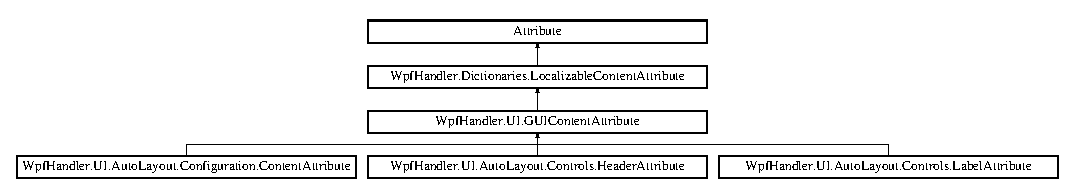
\includegraphics[height=2.170543cm]{d3/dd4/class_wpf_handler_1_1_u_i_1_1_g_u_i_content_attribute}
\end{center}
\end{figure}
\subsection*{Public Member Functions}
\begin{DoxyCompactItemize}
\item 
\mbox{\hyperlink{class_wpf_handler_1_1_u_i_1_1_g_u_i_content_attribute_ac2a5bef97b1df0ab4dfd1e9764710d06}{G\+U\+I\+Content\+Attribute}} ()
\begin{DoxyCompactList}\small\item\em Instiniate new atribute with null G\+UI content. \end{DoxyCompactList}\item 
\mbox{\hyperlink{class_wpf_handler_1_1_u_i_1_1_g_u_i_content_attribute_a26546834215fbd36a79b7811ddc0adfe}{G\+U\+I\+Content\+Attribute}} (string title)
\begin{DoxyCompactList}\small\item\em Auto initialize content with shared title value. \end{DoxyCompactList}\item 
\mbox{\hyperlink{class_wpf_handler_1_1_u_i_1_1_g_u_i_content_attribute_ad64c2fed8f65549ff65ba1bfa3185e05}{G\+U\+I\+Content\+Attribute}} (string title, string description)
\begin{DoxyCompactList}\small\item\em Constructor that allow to set title. \end{DoxyCompactList}\item 
\mbox{\hyperlink{class_wpf_handler_1_1_u_i_1_1_g_u_i_content_attribute_a251d3d3299dcd8fed8ae91e315cf8a1c}{G\+U\+I\+Content\+Attribute}} (string default\+Title, string default\+Description, string decription\+Localization\+Resourse\+Key)
\begin{DoxyCompactList}\small\item\em Initialize all allowed fields. \end{DoxyCompactList}\item 
\mbox{\hyperlink{class_wpf_handler_1_1_u_i_1_1_g_u_i_content_attribute_ac5a1a11874d2effe5743f2a4b5532fd2}{G\+U\+I\+Content\+Attribute}} (string default\+Title, string default\+Description, string title\+Localization\+Resourse\+Key, string decription\+Localization\+Resourse\+Key)
\begin{DoxyCompactList}\small\item\em Initialize all allowed fields. \end{DoxyCompactList}\end{DoxyCompactItemize}
\subsection*{Properties}
\begin{DoxyCompactItemize}
\item 
\mbox{\hyperlink{class_wpf_handler_1_1_u_i_1_1_g_u_i_content}{G\+U\+I\+Content}} \mbox{\hyperlink{class_wpf_handler_1_1_u_i_1_1_g_u_i_content_attribute_a300bccba346680f1baa6812f557209c5}{Content}}\hspace{0.3cm}{\ttfamily  \mbox{[}get, set\mbox{]}}
\begin{DoxyCompactList}\small\item\em Content applied to that G\+UI element. \end{DoxyCompactList}\end{DoxyCompactItemize}


\subsection{Detailed Description}
Define members for attributes focused on managing \mbox{\hyperlink{class_wpf_handler_1_1_u_i_1_1_g_u_i_content}{G\+U\+I\+Content}}. 



\subsection{Constructor \& Destructor Documentation}
\mbox{\Hypertarget{class_wpf_handler_1_1_u_i_1_1_g_u_i_content_attribute_ac2a5bef97b1df0ab4dfd1e9764710d06}\label{class_wpf_handler_1_1_u_i_1_1_g_u_i_content_attribute_ac2a5bef97b1df0ab4dfd1e9764710d06}} 
\index{Wpf\+Handler\+::\+U\+I\+::\+G\+U\+I\+Content\+Attribute@{Wpf\+Handler\+::\+U\+I\+::\+G\+U\+I\+Content\+Attribute}!G\+U\+I\+Content\+Attribute@{G\+U\+I\+Content\+Attribute}}
\index{G\+U\+I\+Content\+Attribute@{G\+U\+I\+Content\+Attribute}!Wpf\+Handler\+::\+U\+I\+::\+G\+U\+I\+Content\+Attribute@{Wpf\+Handler\+::\+U\+I\+::\+G\+U\+I\+Content\+Attribute}}
\subsubsection{\texorpdfstring{G\+U\+I\+Content\+Attribute()}{GUIContentAttribute()}\hspace{0.1cm}{\footnotesize\ttfamily [1/5]}}
{\footnotesize\ttfamily Wpf\+Handler.\+U\+I.\+G\+U\+I\+Content\+Attribute.\+G\+U\+I\+Content\+Attribute (\begin{DoxyParamCaption}{ }\end{DoxyParamCaption})}



Instiniate new atribute with null G\+UI content. 

\mbox{\Hypertarget{class_wpf_handler_1_1_u_i_1_1_g_u_i_content_attribute_a26546834215fbd36a79b7811ddc0adfe}\label{class_wpf_handler_1_1_u_i_1_1_g_u_i_content_attribute_a26546834215fbd36a79b7811ddc0adfe}} 
\index{Wpf\+Handler\+::\+U\+I\+::\+G\+U\+I\+Content\+Attribute@{Wpf\+Handler\+::\+U\+I\+::\+G\+U\+I\+Content\+Attribute}!G\+U\+I\+Content\+Attribute@{G\+U\+I\+Content\+Attribute}}
\index{G\+U\+I\+Content\+Attribute@{G\+U\+I\+Content\+Attribute}!Wpf\+Handler\+::\+U\+I\+::\+G\+U\+I\+Content\+Attribute@{Wpf\+Handler\+::\+U\+I\+::\+G\+U\+I\+Content\+Attribute}}
\subsubsection{\texorpdfstring{G\+U\+I\+Content\+Attribute()}{GUIContentAttribute()}\hspace{0.1cm}{\footnotesize\ttfamily [2/5]}}
{\footnotesize\ttfamily Wpf\+Handler.\+U\+I.\+G\+U\+I\+Content\+Attribute.\+G\+U\+I\+Content\+Attribute (\begin{DoxyParamCaption}\item[{string}]{title }\end{DoxyParamCaption})}



Auto initialize content with shared title value. 


\begin{DoxyParams}{Parameters}
{\em title} & Title that will be showed up into the label.\\
\hline
\end{DoxyParams}


If the title value is null or empty then instiniating \mbox{\hyperlink{class_wpf_handler_1_1_u_i_1_1_g_u_i_content_a9d8259c5a572b9ab33faab8166fc6053}{G\+U\+I\+Content.\+None}}.\mbox{\Hypertarget{class_wpf_handler_1_1_u_i_1_1_g_u_i_content_attribute_ad64c2fed8f65549ff65ba1bfa3185e05}\label{class_wpf_handler_1_1_u_i_1_1_g_u_i_content_attribute_ad64c2fed8f65549ff65ba1bfa3185e05}} 
\index{Wpf\+Handler\+::\+U\+I\+::\+G\+U\+I\+Content\+Attribute@{Wpf\+Handler\+::\+U\+I\+::\+G\+U\+I\+Content\+Attribute}!G\+U\+I\+Content\+Attribute@{G\+U\+I\+Content\+Attribute}}
\index{G\+U\+I\+Content\+Attribute@{G\+U\+I\+Content\+Attribute}!Wpf\+Handler\+::\+U\+I\+::\+G\+U\+I\+Content\+Attribute@{Wpf\+Handler\+::\+U\+I\+::\+G\+U\+I\+Content\+Attribute}}
\subsubsection{\texorpdfstring{G\+U\+I\+Content\+Attribute()}{GUIContentAttribute()}\hspace{0.1cm}{\footnotesize\ttfamily [3/5]}}
{\footnotesize\ttfamily Wpf\+Handler.\+U\+I.\+G\+U\+I\+Content\+Attribute.\+G\+U\+I\+Content\+Attribute (\begin{DoxyParamCaption}\item[{string}]{title,  }\item[{string}]{description }\end{DoxyParamCaption})}



Constructor that allow to set title. 


\begin{DoxyParams}{Parameters}
{\em title} & Title of that element.\\
\hline
{\em description} & Description of that element.\\
\hline
\end{DoxyParams}
\mbox{\Hypertarget{class_wpf_handler_1_1_u_i_1_1_g_u_i_content_attribute_a251d3d3299dcd8fed8ae91e315cf8a1c}\label{class_wpf_handler_1_1_u_i_1_1_g_u_i_content_attribute_a251d3d3299dcd8fed8ae91e315cf8a1c}} 
\index{Wpf\+Handler\+::\+U\+I\+::\+G\+U\+I\+Content\+Attribute@{Wpf\+Handler\+::\+U\+I\+::\+G\+U\+I\+Content\+Attribute}!G\+U\+I\+Content\+Attribute@{G\+U\+I\+Content\+Attribute}}
\index{G\+U\+I\+Content\+Attribute@{G\+U\+I\+Content\+Attribute}!Wpf\+Handler\+::\+U\+I\+::\+G\+U\+I\+Content\+Attribute@{Wpf\+Handler\+::\+U\+I\+::\+G\+U\+I\+Content\+Attribute}}
\subsubsection{\texorpdfstring{G\+U\+I\+Content\+Attribute()}{GUIContentAttribute()}\hspace{0.1cm}{\footnotesize\ttfamily [4/5]}}
{\footnotesize\ttfamily Wpf\+Handler.\+U\+I.\+G\+U\+I\+Content\+Attribute.\+G\+U\+I\+Content\+Attribute (\begin{DoxyParamCaption}\item[{string}]{default\+Title,  }\item[{string}]{default\+Description,  }\item[{string}]{decription\+Localization\+Resourse\+Key }\end{DoxyParamCaption})}



Initialize all allowed fields. 


\begin{DoxyParams}{Parameters}
{\em default\+Title} & Title that would be used by default if localization dictionary not found.\\
\hline
{\em default\+Description} & Default description if localization dictionary not found.\\
\hline
{\em decription\+Localization\+Resourse\+Key} & Key of description content in localized dynamic dictionary.\\
\hline
\end{DoxyParams}
\mbox{\Hypertarget{class_wpf_handler_1_1_u_i_1_1_g_u_i_content_attribute_ac5a1a11874d2effe5743f2a4b5532fd2}\label{class_wpf_handler_1_1_u_i_1_1_g_u_i_content_attribute_ac5a1a11874d2effe5743f2a4b5532fd2}} 
\index{Wpf\+Handler\+::\+U\+I\+::\+G\+U\+I\+Content\+Attribute@{Wpf\+Handler\+::\+U\+I\+::\+G\+U\+I\+Content\+Attribute}!G\+U\+I\+Content\+Attribute@{G\+U\+I\+Content\+Attribute}}
\index{G\+U\+I\+Content\+Attribute@{G\+U\+I\+Content\+Attribute}!Wpf\+Handler\+::\+U\+I\+::\+G\+U\+I\+Content\+Attribute@{Wpf\+Handler\+::\+U\+I\+::\+G\+U\+I\+Content\+Attribute}}
\subsubsection{\texorpdfstring{G\+U\+I\+Content\+Attribute()}{GUIContentAttribute()}\hspace{0.1cm}{\footnotesize\ttfamily [5/5]}}
{\footnotesize\ttfamily Wpf\+Handler.\+U\+I.\+G\+U\+I\+Content\+Attribute.\+G\+U\+I\+Content\+Attribute (\begin{DoxyParamCaption}\item[{string}]{default\+Title,  }\item[{string}]{default\+Description,  }\item[{string}]{title\+Localization\+Resourse\+Key,  }\item[{string}]{decription\+Localization\+Resourse\+Key }\end{DoxyParamCaption})}



Initialize all allowed fields. 


\begin{DoxyParams}{Parameters}
{\em default\+Title} & Title that would be used by default if localization dictionary not found.\\
\hline
{\em default\+Description} & Default description if localization dictionary not found.\\
\hline
{\em title\+Localization\+Resourse\+Key} & Key of title content in localized dynamic dictionary.\\
\hline
{\em decription\+Localization\+Resourse\+Key} & Key of description content in localized dynamic dictionary.\\
\hline
\end{DoxyParams}


\subsection{Property Documentation}
\mbox{\Hypertarget{class_wpf_handler_1_1_u_i_1_1_g_u_i_content_attribute_a300bccba346680f1baa6812f557209c5}\label{class_wpf_handler_1_1_u_i_1_1_g_u_i_content_attribute_a300bccba346680f1baa6812f557209c5}} 
\index{Wpf\+Handler\+::\+U\+I\+::\+G\+U\+I\+Content\+Attribute@{Wpf\+Handler\+::\+U\+I\+::\+G\+U\+I\+Content\+Attribute}!Content@{Content}}
\index{Content@{Content}!Wpf\+Handler\+::\+U\+I\+::\+G\+U\+I\+Content\+Attribute@{Wpf\+Handler\+::\+U\+I\+::\+G\+U\+I\+Content\+Attribute}}
\subsubsection{\texorpdfstring{Content}{Content}}
{\footnotesize\ttfamily \mbox{\hyperlink{class_wpf_handler_1_1_u_i_1_1_g_u_i_content}{G\+U\+I\+Content}} Wpf\+Handler.\+U\+I.\+G\+U\+I\+Content\+Attribute.\+Content\hspace{0.3cm}{\ttfamily [get]}, {\ttfamily [set]}}



Content applied to that G\+UI element. 



The documentation for this class was generated from the following file\+:\begin{DoxyCompactItemize}
\item 
D\+:/\+Work/\+Git\+Hub/wpf-\/handler/\+Wpf\+Handler/\+U\+I/G\+U\+I\+Content\+Attribute.\+cs\end{DoxyCompactItemize}

\hypertarget{class_wpf_handler_1_1_u_i_1_1_controls_1_1_header}{}\section{Wpf\+Handler.\+U\+I.\+Controls.\+Header Class Reference}
\label{class_wpf_handler_1_1_u_i_1_1_controls_1_1_header}\index{Wpf\+Handler.\+U\+I.\+Controls.\+Header@{Wpf\+Handler.\+U\+I.\+Controls.\+Header}}


\mbox{\hyperlink{class_wpf_handler_1_1_u_i_1_1_controls_1_1_header}{Header}}  


Inheritance diagram for Wpf\+Handler.\+U\+I.\+Controls.\+Header\+:\begin{figure}[H]
\begin{center}
\leavevmode
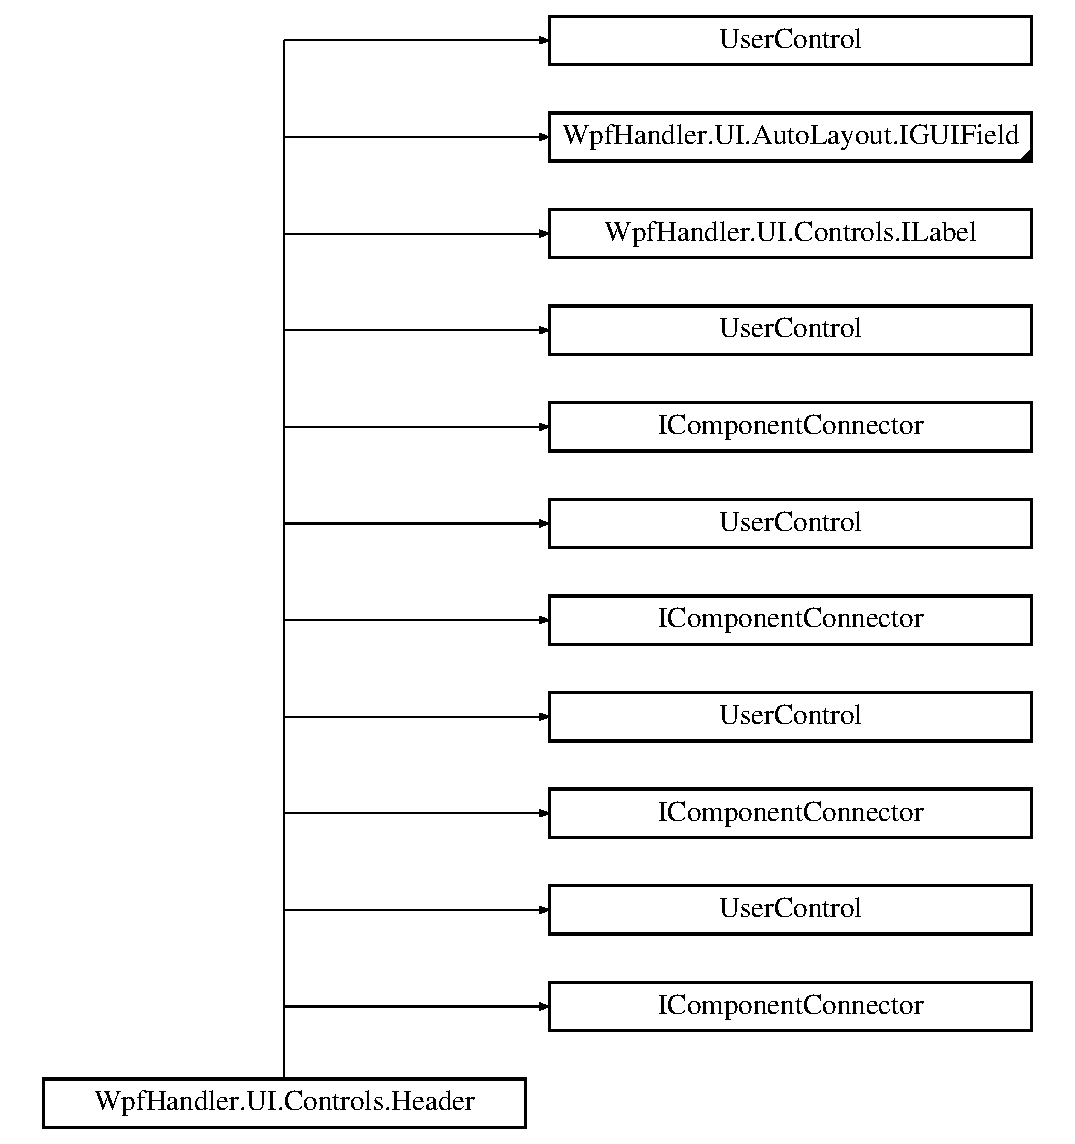
\includegraphics[height=12.000000cm]{d2/dc0/class_wpf_handler_1_1_u_i_1_1_controls_1_1_header}
\end{center}
\end{figure}
\subsection*{Public Member Functions}
\begin{DoxyCompactItemize}
\item 
void \mbox{\hyperlink{class_wpf_handler_1_1_u_i_1_1_controls_1_1_header_a3bc7092e9a7ce867b8f29cad1c1d3f2f}{Initialize\+Component}} ()
\begin{DoxyCompactList}\small\item\em Initialize\+Component \end{DoxyCompactList}\item 
void \mbox{\hyperlink{class_wpf_handler_1_1_u_i_1_1_controls_1_1_header_a3bc7092e9a7ce867b8f29cad1c1d3f2f}{Initialize\+Component}} ()
\begin{DoxyCompactList}\small\item\em Initialize\+Component \end{DoxyCompactList}\item 
void \mbox{\hyperlink{class_wpf_handler_1_1_u_i_1_1_controls_1_1_header_a3bc7092e9a7ce867b8f29cad1c1d3f2f}{Initialize\+Component}} ()
\begin{DoxyCompactList}\small\item\em Initialize\+Component \end{DoxyCompactList}\item 
void \mbox{\hyperlink{class_wpf_handler_1_1_u_i_1_1_controls_1_1_header_a3bc7092e9a7ce867b8f29cad1c1d3f2f}{Initialize\+Component}} ()
\begin{DoxyCompactList}\small\item\em Initialize\+Component \end{DoxyCompactList}\item 
\mbox{\hyperlink{class_wpf_handler_1_1_u_i_1_1_controls_1_1_header_a58551b76c66c4da201070cf01d0561f6}{Header}} ()
\begin{DoxyCompactList}\small\item\em Default costructor. \end{DoxyCompactList}\item 
void \mbox{\hyperlink{class_wpf_handler_1_1_u_i_1_1_controls_1_1_header_a23ac86ea123581ee90d1aa9b6a81dadd}{On\+Layout}} (ref \mbox{\hyperlink{class_wpf_handler_1_1_u_i_1_1_auto_layout_1_1_layout_layer}{Layout\+Layer}} layer, params object\mbox{[}$\,$\mbox{]} args)
\begin{DoxyCompactList}\small\item\em Connecting element to the \mbox{\hyperlink{namespace_wpf_handler_1_1_u_i}{UI}} handler. \end{DoxyCompactList}\end{DoxyCompactItemize}
\subsection*{Static Public Attributes}
\begin{DoxyCompactItemize}
\item 
static readonly Dependency\+Property \mbox{\hyperlink{class_wpf_handler_1_1_u_i_1_1_controls_1_1_header_a69d6de68c4cb8c83f31b15efbd0323dc}{Label\+Property}}
\begin{DoxyCompactList}\small\item\em Bridging X\+A\+ML declaring and the member. \end{DoxyCompactList}\item 
static readonly Dependency\+Property \mbox{\hyperlink{class_wpf_handler_1_1_u_i_1_1_controls_1_1_header_afc03b2a1c85957c525b20e793ce9cfe4}{G\+U\+I\+Content\+Property}}
\begin{DoxyCompactList}\small\item\em Bridging X\+A\+ML declaring and the member. \end{DoxyCompactList}\item 
static readonly Dependency\+Property \mbox{\hyperlink{class_wpf_handler_1_1_u_i_1_1_controls_1_1_header_a8d052187be3a68e9da2d4436bea3b504}{Active\+Property}}
\begin{DoxyCompactList}\small\item\em Bridging X\+A\+ML declaring and the member. \end{DoxyCompactList}\item 
static readonly Dependency\+Property \mbox{\hyperlink{class_wpf_handler_1_1_u_i_1_1_controls_1_1_header_aa3473a8ebaf39118c2ec51ddc0fcfce7}{Arrow\+Visible\+Property}}
\begin{DoxyCompactList}\small\item\em Bridging X\+A\+ML declaring and the member. \end{DoxyCompactList}\end{DoxyCompactItemize}
\subsection*{Package Attributes}
\begin{DoxyCompactItemize}
\item 
\mbox{\Hypertarget{class_wpf_handler_1_1_u_i_1_1_controls_1_1_header_ac6b6eb0ae388af1282a5dde380abd4f1}\label{class_wpf_handler_1_1_u_i_1_1_controls_1_1_header_ac6b6eb0ae388af1282a5dde380abd4f1}} 
\mbox{\hyperlink{class_wpf_handler_1_1_u_i_1_1_controls_1_1_header}{Wpf\+Handler.\+U\+I.\+Controls.\+Header}} {\bfseries main}
\item 
\mbox{\Hypertarget{class_wpf_handler_1_1_u_i_1_1_controls_1_1_header_a0c41a0e112b170298f34dd1afe555466}\label{class_wpf_handler_1_1_u_i_1_1_controls_1_1_header_a0c41a0e112b170298f34dd1afe555466}} 
System.\+Windows.\+Controls.\+Button {\bfseries button}
\item 
\mbox{\Hypertarget{class_wpf_handler_1_1_u_i_1_1_controls_1_1_header_a4dca87c9678237c9b2af0dd3dc0bb2e0}\label{class_wpf_handler_1_1_u_i_1_1_controls_1_1_header_a4dca87c9678237c9b2af0dd3dc0bb2e0}} 
System.\+Windows.\+Controls.\+Canvas {\bfseries list\+Control\+Ui}
\item 
\mbox{\Hypertarget{class_wpf_handler_1_1_u_i_1_1_controls_1_1_header_a457a413551d46e0674c51d22cbc1dd4f}\label{class_wpf_handler_1_1_u_i_1_1_controls_1_1_header_a457a413551d46e0674c51d22cbc1dd4f}} 
System.\+Windows.\+Shapes.\+Polygon {\bfseries list\+Control\+Ui\+\_\+\+Showed}
\item 
\mbox{\Hypertarget{class_wpf_handler_1_1_u_i_1_1_controls_1_1_header_a1fc08ceb38e9267375a64117ea03cfae}\label{class_wpf_handler_1_1_u_i_1_1_controls_1_1_header_a1fc08ceb38e9267375a64117ea03cfae}} 
System.\+Windows.\+Shapes.\+Polygon {\bfseries list\+Control\+Ui\+\_\+\+Hided}
\item 
\mbox{\Hypertarget{class_wpf_handler_1_1_u_i_1_1_controls_1_1_header_ab10ca0ccba374875757330fdd30ddab0}\label{class_wpf_handler_1_1_u_i_1_1_controls_1_1_header_ab10ca0ccba374875757330fdd30ddab0}} 
System.\+Windows.\+Controls.\+Label {\bfseries label}
\end{DoxyCompactItemize}
\subsection*{Properties}
\begin{DoxyCompactItemize}
\item 
Member\+Info \mbox{\hyperlink{class_wpf_handler_1_1_u_i_1_1_controls_1_1_header_a520cdfcc6671c954b6b889f61082244c}{Binded\+Member}}\hspace{0.3cm}{\ttfamily  \mbox{[}get, set\mbox{]}}
\begin{DoxyCompactList}\small\item\em Memeber that will be used as source for the value into \mbox{\hyperlink{namespace_wpf_handler_1_1_u_i}{UI}}. \end{DoxyCompactList}\item 
\mbox{\hyperlink{class_wpf_handler_1_1_u_i_1_1_auto_layout_1_1_layout_layer}{Layout\+Layer}} \mbox{\hyperlink{class_wpf_handler_1_1_u_i_1_1_controls_1_1_header_a3947ddcb07258827b26c25d9ca0f242d}{Child\+Layer}}\hspace{0.3cm}{\ttfamily  \mbox{[}get, set\mbox{]}}
\begin{DoxyCompactList}\small\item\em Layer thst will be managed by that header. \end{DoxyCompactList}\item 
string \mbox{\hyperlink{class_wpf_handler_1_1_u_i_1_1_controls_1_1_header_a6ea05d5b82deba64afc724e79a93275e}{Label}}\hspace{0.3cm}{\ttfamily  \mbox{[}get, set\mbox{]}}
\begin{DoxyCompactList}\small\item\em Text in label field. \end{DoxyCompactList}\item 
bool \mbox{\hyperlink{class_wpf_handler_1_1_u_i_1_1_controls_1_1_header_a020e75c12da978773cd2a3f0089e0644}{Active}}\hspace{0.3cm}{\ttfamily  \mbox{[}get, set\mbox{]}}
\begin{DoxyCompactList}\small\item\em Is this header active. \end{DoxyCompactList}\item 
bool \mbox{\hyperlink{class_wpf_handler_1_1_u_i_1_1_controls_1_1_header_a982c296a72324bf0fab5076cebd60928}{Arrow\+Visible}}\hspace{0.3cm}{\ttfamily  \mbox{[}get, set\mbox{]}}
\begin{DoxyCompactList}\small\item\em Is this header active state arrow is visible. \end{DoxyCompactList}\item 
\mbox{\hyperlink{class_wpf_handler_1_1_u_i_1_1_g_u_i_content}{G\+U\+I\+Content}} \mbox{\hyperlink{class_wpf_handler_1_1_u_i_1_1_controls_1_1_header_a0039e7d4594591d0d9ca1bf99a1ee497}{G\+U\+I\+Content}}\hspace{0.3cm}{\ttfamily  \mbox{[}get, set\mbox{]}}
\begin{DoxyCompactList}\small\item\em Is this header active state arrow is visible. \end{DoxyCompactList}\item 
object \mbox{\hyperlink{class_wpf_handler_1_1_u_i_1_1_controls_1_1_header_a905e42505bb758f31a2178730e41aa19}{Value}}\hspace{0.3cm}{\ttfamily  \mbox{[}get, set\mbox{]}}
\begin{DoxyCompactList}\small\item\em Uniform value of that property. Allow only bool. Deine state of  property. \end{DoxyCompactList}\item 
float \mbox{\hyperlink{class_wpf_handler_1_1_u_i_1_1_controls_1_1_header_a09034cb3d506198643c0d13b4b10cfdb}{Label\+Width}}\hspace{0.3cm}{\ttfamily  \mbox{[}get, set\mbox{]}}
\begin{DoxyCompactList}\small\item\em Not supported. \end{DoxyCompactList}\end{DoxyCompactItemize}
\subsection*{Events}
\begin{DoxyCompactItemize}
\item 
Action$<$ \mbox{\hyperlink{interface_wpf_handler_1_1_u_i_1_1_auto_layout_1_1_i_g_u_i_field}{I\+G\+U\+I\+Field}} $>$ \mbox{\hyperlink{class_wpf_handler_1_1_u_i_1_1_controls_1_1_header_a0934846d1b0bafdabb4997d47fb01b6c}{Value\+Changed}}
\begin{DoxyCompactList}\small\item\em Event that will occure in case if value of the field will be changed. Will cause updating of the Binded\+Member value. \end{DoxyCompactList}\end{DoxyCompactItemize}
\subsection*{Private Member Functions}
\begin{DoxyCompactItemize}
\item 
\mbox{\Hypertarget{class_wpf_handler_1_1_u_i_1_1_controls_1_1_header_a51aa62d103bb6008eb6760c6ff8a9a3d}\label{class_wpf_handler_1_1_u_i_1_1_controls_1_1_header_a51aa62d103bb6008eb6760c6ff8a9a3d}} 
void System.\+Windows.\+Markup.\+I\+Component\+Connector. {\bfseries Connect} (int connection\+Id, object target)
\item 
\mbox{\Hypertarget{class_wpf_handler_1_1_u_i_1_1_controls_1_1_header_a51aa62d103bb6008eb6760c6ff8a9a3d}\label{class_wpf_handler_1_1_u_i_1_1_controls_1_1_header_a51aa62d103bb6008eb6760c6ff8a9a3d}} 
void System.\+Windows.\+Markup.\+I\+Component\+Connector. {\bfseries Connect} (int connection\+Id, object target)
\item 
\mbox{\Hypertarget{class_wpf_handler_1_1_u_i_1_1_controls_1_1_header_a51aa62d103bb6008eb6760c6ff8a9a3d}\label{class_wpf_handler_1_1_u_i_1_1_controls_1_1_header_a51aa62d103bb6008eb6760c6ff8a9a3d}} 
void System.\+Windows.\+Markup.\+I\+Component\+Connector. {\bfseries Connect} (int connection\+Id, object target)
\item 
\mbox{\Hypertarget{class_wpf_handler_1_1_u_i_1_1_controls_1_1_header_a51aa62d103bb6008eb6760c6ff8a9a3d}\label{class_wpf_handler_1_1_u_i_1_1_controls_1_1_header_a51aa62d103bb6008eb6760c6ff8a9a3d}} 
void System.\+Windows.\+Markup.\+I\+Component\+Connector. {\bfseries Connect} (int connection\+Id, object target)
\item 
void \mbox{\hyperlink{class_wpf_handler_1_1_u_i_1_1_controls_1_1_header_ae986415a1ad448e5d3a6c5b88504f11d}{Button\+\_\+\+Click}} (object sender, Routed\+Event\+Args e)
\begin{DoxyCompactList}\small\item\em Occurs when layer state button was clicked. \end{DoxyCompactList}\end{DoxyCompactItemize}
\subsection*{Private Attributes}
\begin{DoxyCompactItemize}
\item 
\mbox{\Hypertarget{class_wpf_handler_1_1_u_i_1_1_controls_1_1_header_a90429ce83ea8bb00102a0e1bd2c660c1}\label{class_wpf_handler_1_1_u_i_1_1_controls_1_1_header_a90429ce83ea8bb00102a0e1bd2c660c1}} 
bool {\bfseries \+\_\+content\+Loaded}
\end{DoxyCompactItemize}


\subsection{Detailed Description}
\mbox{\hyperlink{class_wpf_handler_1_1_u_i_1_1_controls_1_1_header}{Header}} 

Interaction logic for Header.\+xaml 

\subsection{Constructor \& Destructor Documentation}
\mbox{\Hypertarget{class_wpf_handler_1_1_u_i_1_1_controls_1_1_header_a58551b76c66c4da201070cf01d0561f6}\label{class_wpf_handler_1_1_u_i_1_1_controls_1_1_header_a58551b76c66c4da201070cf01d0561f6}} 
\index{Wpf\+Handler\+::\+U\+I\+::\+Controls\+::\+Header@{Wpf\+Handler\+::\+U\+I\+::\+Controls\+::\+Header}!Header@{Header}}
\index{Header@{Header}!Wpf\+Handler\+::\+U\+I\+::\+Controls\+::\+Header@{Wpf\+Handler\+::\+U\+I\+::\+Controls\+::\+Header}}
\subsubsection{\texorpdfstring{Header()}{Header()}}
{\footnotesize\ttfamily Wpf\+Handler.\+U\+I.\+Controls.\+Header.\+Header (\begin{DoxyParamCaption}{ }\end{DoxyParamCaption})}



Default costructor. 



\subsection{Member Function Documentation}
\mbox{\Hypertarget{class_wpf_handler_1_1_u_i_1_1_controls_1_1_header_ae986415a1ad448e5d3a6c5b88504f11d}\label{class_wpf_handler_1_1_u_i_1_1_controls_1_1_header_ae986415a1ad448e5d3a6c5b88504f11d}} 
\index{Wpf\+Handler\+::\+U\+I\+::\+Controls\+::\+Header@{Wpf\+Handler\+::\+U\+I\+::\+Controls\+::\+Header}!Button\+\_\+\+Click@{Button\+\_\+\+Click}}
\index{Button\+\_\+\+Click@{Button\+\_\+\+Click}!Wpf\+Handler\+::\+U\+I\+::\+Controls\+::\+Header@{Wpf\+Handler\+::\+U\+I\+::\+Controls\+::\+Header}}
\subsubsection{\texorpdfstring{Button\+\_\+\+Click()}{Button\_Click()}}
{\footnotesize\ttfamily void Wpf\+Handler.\+U\+I.\+Controls.\+Header.\+Button\+\_\+\+Click (\begin{DoxyParamCaption}\item[{object}]{sender,  }\item[{Routed\+Event\+Args}]{e }\end{DoxyParamCaption})\hspace{0.3cm}{\ttfamily [private]}}



Occurs when layer state button was clicked. 


\begin{DoxyParams}{Parameters}
{\em sender} & \\
\hline
{\em e} & \\
\hline
\end{DoxyParams}
\mbox{\Hypertarget{class_wpf_handler_1_1_u_i_1_1_controls_1_1_header_a3bc7092e9a7ce867b8f29cad1c1d3f2f}\label{class_wpf_handler_1_1_u_i_1_1_controls_1_1_header_a3bc7092e9a7ce867b8f29cad1c1d3f2f}} 
\index{Wpf\+Handler\+::\+U\+I\+::\+Controls\+::\+Header@{Wpf\+Handler\+::\+U\+I\+::\+Controls\+::\+Header}!Initialize\+Component@{Initialize\+Component}}
\index{Initialize\+Component@{Initialize\+Component}!Wpf\+Handler\+::\+U\+I\+::\+Controls\+::\+Header@{Wpf\+Handler\+::\+U\+I\+::\+Controls\+::\+Header}}
\subsubsection{\texorpdfstring{Initialize\+Component()}{InitializeComponent()}\hspace{0.1cm}{\footnotesize\ttfamily [1/4]}}
{\footnotesize\ttfamily void Wpf\+Handler.\+U\+I.\+Controls.\+Header.\+Initialize\+Component (\begin{DoxyParamCaption}{ }\end{DoxyParamCaption})}



Initialize\+Component 

\mbox{\Hypertarget{class_wpf_handler_1_1_u_i_1_1_controls_1_1_header_a3bc7092e9a7ce867b8f29cad1c1d3f2f}\label{class_wpf_handler_1_1_u_i_1_1_controls_1_1_header_a3bc7092e9a7ce867b8f29cad1c1d3f2f}} 
\index{Wpf\+Handler\+::\+U\+I\+::\+Controls\+::\+Header@{Wpf\+Handler\+::\+U\+I\+::\+Controls\+::\+Header}!Initialize\+Component@{Initialize\+Component}}
\index{Initialize\+Component@{Initialize\+Component}!Wpf\+Handler\+::\+U\+I\+::\+Controls\+::\+Header@{Wpf\+Handler\+::\+U\+I\+::\+Controls\+::\+Header}}
\subsubsection{\texorpdfstring{Initialize\+Component()}{InitializeComponent()}\hspace{0.1cm}{\footnotesize\ttfamily [2/4]}}
{\footnotesize\ttfamily void Wpf\+Handler.\+U\+I.\+Controls.\+Header.\+Initialize\+Component (\begin{DoxyParamCaption}{ }\end{DoxyParamCaption})}



Initialize\+Component 

\mbox{\Hypertarget{class_wpf_handler_1_1_u_i_1_1_controls_1_1_header_a3bc7092e9a7ce867b8f29cad1c1d3f2f}\label{class_wpf_handler_1_1_u_i_1_1_controls_1_1_header_a3bc7092e9a7ce867b8f29cad1c1d3f2f}} 
\index{Wpf\+Handler\+::\+U\+I\+::\+Controls\+::\+Header@{Wpf\+Handler\+::\+U\+I\+::\+Controls\+::\+Header}!Initialize\+Component@{Initialize\+Component}}
\index{Initialize\+Component@{Initialize\+Component}!Wpf\+Handler\+::\+U\+I\+::\+Controls\+::\+Header@{Wpf\+Handler\+::\+U\+I\+::\+Controls\+::\+Header}}
\subsubsection{\texorpdfstring{Initialize\+Component()}{InitializeComponent()}\hspace{0.1cm}{\footnotesize\ttfamily [3/4]}}
{\footnotesize\ttfamily void Wpf\+Handler.\+U\+I.\+Controls.\+Header.\+Initialize\+Component (\begin{DoxyParamCaption}{ }\end{DoxyParamCaption})}



Initialize\+Component 

\mbox{\Hypertarget{class_wpf_handler_1_1_u_i_1_1_controls_1_1_header_a3bc7092e9a7ce867b8f29cad1c1d3f2f}\label{class_wpf_handler_1_1_u_i_1_1_controls_1_1_header_a3bc7092e9a7ce867b8f29cad1c1d3f2f}} 
\index{Wpf\+Handler\+::\+U\+I\+::\+Controls\+::\+Header@{Wpf\+Handler\+::\+U\+I\+::\+Controls\+::\+Header}!Initialize\+Component@{Initialize\+Component}}
\index{Initialize\+Component@{Initialize\+Component}!Wpf\+Handler\+::\+U\+I\+::\+Controls\+::\+Header@{Wpf\+Handler\+::\+U\+I\+::\+Controls\+::\+Header}}
\subsubsection{\texorpdfstring{Initialize\+Component()}{InitializeComponent()}\hspace{0.1cm}{\footnotesize\ttfamily [4/4]}}
{\footnotesize\ttfamily void Wpf\+Handler.\+U\+I.\+Controls.\+Header.\+Initialize\+Component (\begin{DoxyParamCaption}{ }\end{DoxyParamCaption})}



Initialize\+Component 

\mbox{\Hypertarget{class_wpf_handler_1_1_u_i_1_1_controls_1_1_header_a23ac86ea123581ee90d1aa9b6a81dadd}\label{class_wpf_handler_1_1_u_i_1_1_controls_1_1_header_a23ac86ea123581ee90d1aa9b6a81dadd}} 
\index{Wpf\+Handler\+::\+U\+I\+::\+Controls\+::\+Header@{Wpf\+Handler\+::\+U\+I\+::\+Controls\+::\+Header}!On\+Layout@{On\+Layout}}
\index{On\+Layout@{On\+Layout}!Wpf\+Handler\+::\+U\+I\+::\+Controls\+::\+Header@{Wpf\+Handler\+::\+U\+I\+::\+Controls\+::\+Header}}
\subsubsection{\texorpdfstring{On\+Layout()}{OnLayout()}}
{\footnotesize\ttfamily void Wpf\+Handler.\+U\+I.\+Controls.\+Header.\+On\+Layout (\begin{DoxyParamCaption}\item[{ref \mbox{\hyperlink{class_wpf_handler_1_1_u_i_1_1_auto_layout_1_1_layout_layer}{Layout\+Layer}}}]{layer,  }\item[{params object \mbox{[}$\,$\mbox{]}}]{args }\end{DoxyParamCaption})}



Connecting element to the \mbox{\hyperlink{namespace_wpf_handler_1_1_u_i}{UI}} handler. 


\begin{DoxyParams}{Parameters}
{\em layer} & Target \mbox{\hyperlink{namespace_wpf_handler_1_1_u_i}{UI}} layer.\\
\hline
{\em args} & Must contains\+: U\+I\+Descriptor and Member\+Info\\
\hline
\end{DoxyParams}


Implements \mbox{\hyperlink{interface_wpf_handler_1_1_u_i_1_1_auto_layout_1_1_i_g_u_i_element_a0ff16956f8e8187d51e1b36b6b9f894e}{Wpf\+Handler.\+U\+I.\+Auto\+Layout.\+I\+G\+U\+I\+Element}}.



\subsection{Member Data Documentation}
\mbox{\Hypertarget{class_wpf_handler_1_1_u_i_1_1_controls_1_1_header_a8d052187be3a68e9da2d4436bea3b504}\label{class_wpf_handler_1_1_u_i_1_1_controls_1_1_header_a8d052187be3a68e9da2d4436bea3b504}} 
\index{Wpf\+Handler\+::\+U\+I\+::\+Controls\+::\+Header@{Wpf\+Handler\+::\+U\+I\+::\+Controls\+::\+Header}!Active\+Property@{Active\+Property}}
\index{Active\+Property@{Active\+Property}!Wpf\+Handler\+::\+U\+I\+::\+Controls\+::\+Header@{Wpf\+Handler\+::\+U\+I\+::\+Controls\+::\+Header}}
\subsubsection{\texorpdfstring{Active\+Property}{ActiveProperty}}
{\footnotesize\ttfamily readonly Dependency\+Property Wpf\+Handler.\+U\+I.\+Controls.\+Header.\+Active\+Property\hspace{0.3cm}{\ttfamily [static]}}

{\bfseries Initial value\+:}
\begin{DoxyCode}
= DependencyProperty.Register(
            \textcolor{stringliteral}{"Active"}, typeof(\textcolor{keywordtype}{bool}), typeof(\mbox{\hyperlink{class_wpf_handler_1_1_u_i_1_1_controls_1_1_header_a58551b76c66c4da201070cf01d0561f6}{Header}}), \textcolor{keyword}{new} PropertyMetadata(\textcolor{keyword}{true}))
\end{DoxyCode}


Bridging X\+A\+ML declaring and the member. 

\mbox{\Hypertarget{class_wpf_handler_1_1_u_i_1_1_controls_1_1_header_aa3473a8ebaf39118c2ec51ddc0fcfce7}\label{class_wpf_handler_1_1_u_i_1_1_controls_1_1_header_aa3473a8ebaf39118c2ec51ddc0fcfce7}} 
\index{Wpf\+Handler\+::\+U\+I\+::\+Controls\+::\+Header@{Wpf\+Handler\+::\+U\+I\+::\+Controls\+::\+Header}!Arrow\+Visible\+Property@{Arrow\+Visible\+Property}}
\index{Arrow\+Visible\+Property@{Arrow\+Visible\+Property}!Wpf\+Handler\+::\+U\+I\+::\+Controls\+::\+Header@{Wpf\+Handler\+::\+U\+I\+::\+Controls\+::\+Header}}
\subsubsection{\texorpdfstring{Arrow\+Visible\+Property}{ArrowVisibleProperty}}
{\footnotesize\ttfamily readonly Dependency\+Property Wpf\+Handler.\+U\+I.\+Controls.\+Header.\+Arrow\+Visible\+Property\hspace{0.3cm}{\ttfamily [static]}}

{\bfseries Initial value\+:}
\begin{DoxyCode}
= DependencyProperty.Register(
            \textcolor{stringliteral}{"ArrowVisible"}, typeof(\textcolor{keywordtype}{bool}), typeof(\mbox{\hyperlink{class_wpf_handler_1_1_u_i_1_1_controls_1_1_header_a58551b76c66c4da201070cf01d0561f6}{Header}}), \textcolor{keyword}{new} PropertyMetadata(\textcolor{keyword}{true}))
\end{DoxyCode}


Bridging X\+A\+ML declaring and the member. 

\mbox{\Hypertarget{class_wpf_handler_1_1_u_i_1_1_controls_1_1_header_afc03b2a1c85957c525b20e793ce9cfe4}\label{class_wpf_handler_1_1_u_i_1_1_controls_1_1_header_afc03b2a1c85957c525b20e793ce9cfe4}} 
\index{Wpf\+Handler\+::\+U\+I\+::\+Controls\+::\+Header@{Wpf\+Handler\+::\+U\+I\+::\+Controls\+::\+Header}!G\+U\+I\+Content\+Property@{G\+U\+I\+Content\+Property}}
\index{G\+U\+I\+Content\+Property@{G\+U\+I\+Content\+Property}!Wpf\+Handler\+::\+U\+I\+::\+Controls\+::\+Header@{Wpf\+Handler\+::\+U\+I\+::\+Controls\+::\+Header}}
\subsubsection{\texorpdfstring{G\+U\+I\+Content\+Property}{GUIContentProperty}}
{\footnotesize\ttfamily readonly Dependency\+Property Wpf\+Handler.\+U\+I.\+Controls.\+Header.\+G\+U\+I\+Content\+Property\hspace{0.3cm}{\ttfamily [static]}}

{\bfseries Initial value\+:}
\begin{DoxyCode}
= DependencyProperty.Register(
            \textcolor{stringliteral}{"GUIContent"}, typeof(\mbox{\hyperlink{class_wpf_handler_1_1_u_i_1_1_controls_1_1_header_a0039e7d4594591d0d9ca1bf99a1ee497}{GUIContent}}), typeof(\mbox{\hyperlink{class_wpf_handler_1_1_u_i_1_1_controls_1_1_header_a58551b76c66c4da201070cf01d0561f6}{Header}}))
\end{DoxyCode}


Bridging X\+A\+ML declaring and the member. 

\mbox{\Hypertarget{class_wpf_handler_1_1_u_i_1_1_controls_1_1_header_a69d6de68c4cb8c83f31b15efbd0323dc}\label{class_wpf_handler_1_1_u_i_1_1_controls_1_1_header_a69d6de68c4cb8c83f31b15efbd0323dc}} 
\index{Wpf\+Handler\+::\+U\+I\+::\+Controls\+::\+Header@{Wpf\+Handler\+::\+U\+I\+::\+Controls\+::\+Header}!Label\+Property@{Label\+Property}}
\index{Label\+Property@{Label\+Property}!Wpf\+Handler\+::\+U\+I\+::\+Controls\+::\+Header@{Wpf\+Handler\+::\+U\+I\+::\+Controls\+::\+Header}}
\subsubsection{\texorpdfstring{Label\+Property}{LabelProperty}}
{\footnotesize\ttfamily readonly Dependency\+Property Wpf\+Handler.\+U\+I.\+Controls.\+Header.\+Label\+Property\hspace{0.3cm}{\ttfamily [static]}}

{\bfseries Initial value\+:}
\begin{DoxyCode}
= DependencyProperty.Register(
            \textcolor{stringliteral}{"Label"}, typeof(\textcolor{keywordtype}{string}), typeof(\mbox{\hyperlink{class_wpf_handler_1_1_u_i_1_1_controls_1_1_header_a58551b76c66c4da201070cf01d0561f6}{Header}}), \textcolor{keyword}{new} PropertyMetadata(\textcolor{stringliteral}{"Sample"}))
\end{DoxyCode}


Bridging X\+A\+ML declaring and the member. 



\subsection{Property Documentation}
\mbox{\Hypertarget{class_wpf_handler_1_1_u_i_1_1_controls_1_1_header_a020e75c12da978773cd2a3f0089e0644}\label{class_wpf_handler_1_1_u_i_1_1_controls_1_1_header_a020e75c12da978773cd2a3f0089e0644}} 
\index{Wpf\+Handler\+::\+U\+I\+::\+Controls\+::\+Header@{Wpf\+Handler\+::\+U\+I\+::\+Controls\+::\+Header}!Active@{Active}}
\index{Active@{Active}!Wpf\+Handler\+::\+U\+I\+::\+Controls\+::\+Header@{Wpf\+Handler\+::\+U\+I\+::\+Controls\+::\+Header}}
\subsubsection{\texorpdfstring{Active}{Active}}
{\footnotesize\ttfamily bool Wpf\+Handler.\+U\+I.\+Controls.\+Header.\+Active\hspace{0.3cm}{\ttfamily [get]}, {\ttfamily [set]}}



Is this header active. 

\mbox{\Hypertarget{class_wpf_handler_1_1_u_i_1_1_controls_1_1_header_a982c296a72324bf0fab5076cebd60928}\label{class_wpf_handler_1_1_u_i_1_1_controls_1_1_header_a982c296a72324bf0fab5076cebd60928}} 
\index{Wpf\+Handler\+::\+U\+I\+::\+Controls\+::\+Header@{Wpf\+Handler\+::\+U\+I\+::\+Controls\+::\+Header}!Arrow\+Visible@{Arrow\+Visible}}
\index{Arrow\+Visible@{Arrow\+Visible}!Wpf\+Handler\+::\+U\+I\+::\+Controls\+::\+Header@{Wpf\+Handler\+::\+U\+I\+::\+Controls\+::\+Header}}
\subsubsection{\texorpdfstring{Arrow\+Visible}{ArrowVisible}}
{\footnotesize\ttfamily bool Wpf\+Handler.\+U\+I.\+Controls.\+Header.\+Arrow\+Visible\hspace{0.3cm}{\ttfamily [get]}, {\ttfamily [set]}}



Is this header active state arrow is visible. 

\mbox{\Hypertarget{class_wpf_handler_1_1_u_i_1_1_controls_1_1_header_a520cdfcc6671c954b6b889f61082244c}\label{class_wpf_handler_1_1_u_i_1_1_controls_1_1_header_a520cdfcc6671c954b6b889f61082244c}} 
\index{Wpf\+Handler\+::\+U\+I\+::\+Controls\+::\+Header@{Wpf\+Handler\+::\+U\+I\+::\+Controls\+::\+Header}!Binded\+Member@{Binded\+Member}}
\index{Binded\+Member@{Binded\+Member}!Wpf\+Handler\+::\+U\+I\+::\+Controls\+::\+Header@{Wpf\+Handler\+::\+U\+I\+::\+Controls\+::\+Header}}
\subsubsection{\texorpdfstring{Binded\+Member}{BindedMember}}
{\footnotesize\ttfamily Member\+Info Wpf\+Handler.\+U\+I.\+Controls.\+Header.\+Binded\+Member\hspace{0.3cm}{\ttfamily [get]}, {\ttfamily [set]}}



Memeber that will be used as source for the value into \mbox{\hyperlink{namespace_wpf_handler_1_1_u_i}{UI}}. 

\mbox{\Hypertarget{class_wpf_handler_1_1_u_i_1_1_controls_1_1_header_a3947ddcb07258827b26c25d9ca0f242d}\label{class_wpf_handler_1_1_u_i_1_1_controls_1_1_header_a3947ddcb07258827b26c25d9ca0f242d}} 
\index{Wpf\+Handler\+::\+U\+I\+::\+Controls\+::\+Header@{Wpf\+Handler\+::\+U\+I\+::\+Controls\+::\+Header}!Child\+Layer@{Child\+Layer}}
\index{Child\+Layer@{Child\+Layer}!Wpf\+Handler\+::\+U\+I\+::\+Controls\+::\+Header@{Wpf\+Handler\+::\+U\+I\+::\+Controls\+::\+Header}}
\subsubsection{\texorpdfstring{Child\+Layer}{ChildLayer}}
{\footnotesize\ttfamily \mbox{\hyperlink{class_wpf_handler_1_1_u_i_1_1_auto_layout_1_1_layout_layer}{Layout\+Layer}} Wpf\+Handler.\+U\+I.\+Controls.\+Header.\+Child\+Layer\hspace{0.3cm}{\ttfamily [get]}, {\ttfamily [set]}}



Layer thst will be managed by that header. 

\mbox{\Hypertarget{class_wpf_handler_1_1_u_i_1_1_controls_1_1_header_a0039e7d4594591d0d9ca1bf99a1ee497}\label{class_wpf_handler_1_1_u_i_1_1_controls_1_1_header_a0039e7d4594591d0d9ca1bf99a1ee497}} 
\index{Wpf\+Handler\+::\+U\+I\+::\+Controls\+::\+Header@{Wpf\+Handler\+::\+U\+I\+::\+Controls\+::\+Header}!G\+U\+I\+Content@{G\+U\+I\+Content}}
\index{G\+U\+I\+Content@{G\+U\+I\+Content}!Wpf\+Handler\+::\+U\+I\+::\+Controls\+::\+Header@{Wpf\+Handler\+::\+U\+I\+::\+Controls\+::\+Header}}
\subsubsection{\texorpdfstring{G\+U\+I\+Content}{GUIContent}}
{\footnotesize\ttfamily \mbox{\hyperlink{class_wpf_handler_1_1_u_i_1_1_g_u_i_content}{G\+U\+I\+Content}} Wpf\+Handler.\+U\+I.\+Controls.\+Header.\+G\+U\+I\+Content\hspace{0.3cm}{\ttfamily [get]}, {\ttfamily [set]}}



Is this header active state arrow is visible. 

\mbox{\Hypertarget{class_wpf_handler_1_1_u_i_1_1_controls_1_1_header_a6ea05d5b82deba64afc724e79a93275e}\label{class_wpf_handler_1_1_u_i_1_1_controls_1_1_header_a6ea05d5b82deba64afc724e79a93275e}} 
\index{Wpf\+Handler\+::\+U\+I\+::\+Controls\+::\+Header@{Wpf\+Handler\+::\+U\+I\+::\+Controls\+::\+Header}!Label@{Label}}
\index{Label@{Label}!Wpf\+Handler\+::\+U\+I\+::\+Controls\+::\+Header@{Wpf\+Handler\+::\+U\+I\+::\+Controls\+::\+Header}}
\subsubsection{\texorpdfstring{Label}{Label}}
{\footnotesize\ttfamily string Wpf\+Handler.\+U\+I.\+Controls.\+Header.\+Label\hspace{0.3cm}{\ttfamily [get]}, {\ttfamily [set]}}



Text in label field. 

\mbox{\Hypertarget{class_wpf_handler_1_1_u_i_1_1_controls_1_1_header_a09034cb3d506198643c0d13b4b10cfdb}\label{class_wpf_handler_1_1_u_i_1_1_controls_1_1_header_a09034cb3d506198643c0d13b4b10cfdb}} 
\index{Wpf\+Handler\+::\+U\+I\+::\+Controls\+::\+Header@{Wpf\+Handler\+::\+U\+I\+::\+Controls\+::\+Header}!Label\+Width@{Label\+Width}}
\index{Label\+Width@{Label\+Width}!Wpf\+Handler\+::\+U\+I\+::\+Controls\+::\+Header@{Wpf\+Handler\+::\+U\+I\+::\+Controls\+::\+Header}}
\subsubsection{\texorpdfstring{Label\+Width}{LabelWidth}}
{\footnotesize\ttfamily float Wpf\+Handler.\+U\+I.\+Controls.\+Header.\+Label\+Width\hspace{0.3cm}{\ttfamily [get]}, {\ttfamily [set]}}



Not supported. 

\mbox{\Hypertarget{class_wpf_handler_1_1_u_i_1_1_controls_1_1_header_a905e42505bb758f31a2178730e41aa19}\label{class_wpf_handler_1_1_u_i_1_1_controls_1_1_header_a905e42505bb758f31a2178730e41aa19}} 
\index{Wpf\+Handler\+::\+U\+I\+::\+Controls\+::\+Header@{Wpf\+Handler\+::\+U\+I\+::\+Controls\+::\+Header}!Value@{Value}}
\index{Value@{Value}!Wpf\+Handler\+::\+U\+I\+::\+Controls\+::\+Header@{Wpf\+Handler\+::\+U\+I\+::\+Controls\+::\+Header}}
\subsubsection{\texorpdfstring{Value}{Value}}
{\footnotesize\ttfamily object Wpf\+Handler.\+U\+I.\+Controls.\+Header.\+Value\hspace{0.3cm}{\ttfamily [get]}, {\ttfamily [set]}}



Uniform value of that property. Allow only bool. Deine state of  property. 



\subsection{Event Documentation}
\mbox{\Hypertarget{class_wpf_handler_1_1_u_i_1_1_controls_1_1_header_a0934846d1b0bafdabb4997d47fb01b6c}\label{class_wpf_handler_1_1_u_i_1_1_controls_1_1_header_a0934846d1b0bafdabb4997d47fb01b6c}} 
\index{Wpf\+Handler\+::\+U\+I\+::\+Controls\+::\+Header@{Wpf\+Handler\+::\+U\+I\+::\+Controls\+::\+Header}!Value\+Changed@{Value\+Changed}}
\index{Value\+Changed@{Value\+Changed}!Wpf\+Handler\+::\+U\+I\+::\+Controls\+::\+Header@{Wpf\+Handler\+::\+U\+I\+::\+Controls\+::\+Header}}
\subsubsection{\texorpdfstring{Value\+Changed}{ValueChanged}}
{\footnotesize\ttfamily Action$<$\mbox{\hyperlink{interface_wpf_handler_1_1_u_i_1_1_auto_layout_1_1_i_g_u_i_field}{I\+G\+U\+I\+Field}}$>$ Wpf\+Handler.\+U\+I.\+Controls.\+Header.\+Value\+Changed}



Event that will occure in case if value of the field will be changed. Will cause updating of the Binded\+Member value. 



The documentation for this class was generated from the following files\+:\begin{DoxyCompactItemize}
\item 
D\+:/\+Work/\+Git\+Hub/wpf-\/handler/\+Wpf\+Handler/obj/\+Debug/\+U\+I/\+Controls/Header.\+g.\+cs\item 
D\+:/\+Work/\+Git\+Hub/wpf-\/handler/\+Wpf\+Handler/obj/\+Debug/\+U\+I/\+Controls/Header.\+g.\+i.\+cs\item 
D\+:/\+Work/\+Git\+Hub/wpf-\/handler/\+Wpf\+Handler/\+U\+I/\+Controls/Header.\+xaml.\+cs\end{DoxyCompactItemize}

\hypertarget{class_wpf_handler_1_1_u_i_1_1_auto_layout_1_1_controls_1_1_header_attribute}{}\section{Wpf\+Handler.\+U\+I.\+Auto\+Layout.\+Controls.\+Header\+Attribute Class Reference}
\label{class_wpf_handler_1_1_u_i_1_1_auto_layout_1_1_controls_1_1_header_attribute}\index{Wpf\+Handler.\+U\+I.\+Auto\+Layout.\+Controls.\+Header\+Attribute@{Wpf\+Handler.\+U\+I.\+Auto\+Layout.\+Controls.\+Header\+Attribute}}


Added header block element to \mbox{\hyperlink{namespace_wpf_handler_1_1_u_i}{UI}}.  


Inheritance diagram for Wpf\+Handler.\+U\+I.\+Auto\+Layout.\+Controls.\+Header\+Attribute\+:\begin{figure}[H]
\begin{center}
\leavevmode
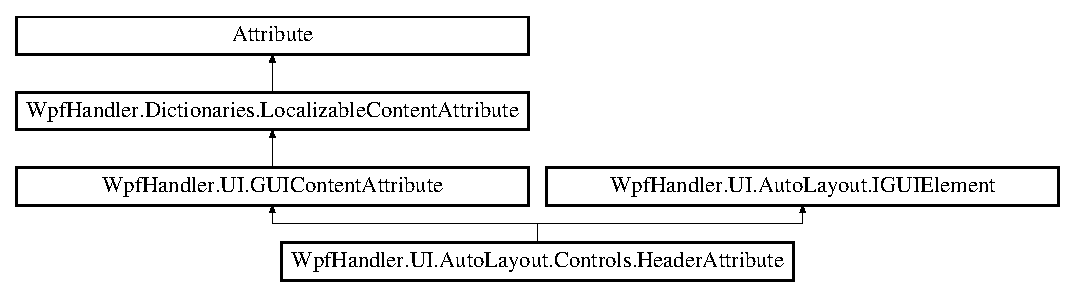
\includegraphics[height=3.544304cm]{d1/d32/class_wpf_handler_1_1_u_i_1_1_auto_layout_1_1_controls_1_1_header_attribute}
\end{center}
\end{figure}
\subsection*{Public Member Functions}
\begin{DoxyCompactItemize}
\item 
\mbox{\hyperlink{class_wpf_handler_1_1_u_i_1_1_auto_layout_1_1_controls_1_1_header_attribute_a0c0c74638fa9192803be651427641a7c}{Header\+Attribute}} (string title)
\begin{DoxyCompactList}\small\item\em Auto initialize content with shared title value. \end{DoxyCompactList}\item 
\mbox{\hyperlink{class_wpf_handler_1_1_u_i_1_1_auto_layout_1_1_controls_1_1_header_attribute_aa89774276da07f96c045d13506488df3}{Header\+Attribute}} (string title, string description)
\begin{DoxyCompactList}\small\item\em Constructor that allow to set title. \end{DoxyCompactList}\item 
\mbox{\hyperlink{class_wpf_handler_1_1_u_i_1_1_auto_layout_1_1_controls_1_1_header_attribute_ac3e75023735c59f6cb90a2f117c02427}{Header\+Attribute}} (string default\+Title, string default\+Description, string decription\+Localization\+Resourse\+Key)
\begin{DoxyCompactList}\small\item\em Initialize all allowed fields. \end{DoxyCompactList}\item 
\mbox{\hyperlink{class_wpf_handler_1_1_u_i_1_1_auto_layout_1_1_controls_1_1_header_attribute_a0ababe608741f8a08b2bcb9a31c32911}{Header\+Attribute}} (string default\+Title, string default\+Description, string title\+Localization\+Resourse\+Key, string decription\+Localization\+Resourse\+Key)
\begin{DoxyCompactList}\small\item\em Initialize all allowed fields. \end{DoxyCompactList}\item 
virtual void \mbox{\hyperlink{class_wpf_handler_1_1_u_i_1_1_auto_layout_1_1_controls_1_1_header_attribute_a837805f9b975447e7cf5663119189c37}{On\+Layout}} (ref \mbox{\hyperlink{class_wpf_handler_1_1_u_i_1_1_auto_layout_1_1_layout_layer}{Layout\+Layer}} layer, params object\mbox{[}$\,$\mbox{]} args)
\begin{DoxyCompactList}\small\item\em Spawning Header \mbox{\hyperlink{namespace_wpf_handler_1_1_u_i}{UI}} elements un shared layer. Connecting to the shared member. \end{DoxyCompactList}\item 
override void \mbox{\hyperlink{class_wpf_handler_1_1_u_i_1_1_auto_layout_1_1_controls_1_1_header_attribute_ae2587a69606cda16cc87e901140f113a}{Languages\+Dictionaries\+Updated}} ()
\begin{DoxyCompactList}\small\item\em T\+O\+DO\+: Callback that occurs when content dictionaries are reloaded. Updating header\textquotesingle{}s content. \end{DoxyCompactList}\end{DoxyCompactItemize}
\subsection*{Properties}
\begin{DoxyCompactItemize}
\item 
bool \mbox{\hyperlink{class_wpf_handler_1_1_u_i_1_1_auto_layout_1_1_controls_1_1_header_attribute_a37e39441398bd5aa132da26eb23e9349}{Default\+State}} = true\hspace{0.3cm}{\ttfamily  \mbox{[}get, set\mbox{]}}
\begin{DoxyCompactList}\small\item\em Default state that will applied to the spawned \mbox{\hyperlink{namespace_wpf_handler_1_1_u_i}{UI}} element. \end{DoxyCompactList}\item 
\mbox{\hyperlink{class_wpf_handler_1_1_u_i_1_1_controls_1_1_header}{U\+I.\+Controls.\+Header}} \mbox{\hyperlink{class_wpf_handler_1_1_u_i_1_1_auto_layout_1_1_controls_1_1_header_attribute_a27af4560ad16335bf2c210692949c1c5}{Binded\+UI}}\hspace{0.3cm}{\ttfamily  \mbox{[}get, protected set\mbox{]}}
\begin{DoxyCompactList}\small\item\em Instiniated \mbox{\hyperlink{namespace_wpf_handler_1_1_u_i}{UI}} element. \end{DoxyCompactList}\end{DoxyCompactItemize}


\subsection{Detailed Description}
Added header block element to \mbox{\hyperlink{namespace_wpf_handler_1_1_u_i}{UI}}. 



\subsection{Constructor \& Destructor Documentation}
\mbox{\Hypertarget{class_wpf_handler_1_1_u_i_1_1_auto_layout_1_1_controls_1_1_header_attribute_a0c0c74638fa9192803be651427641a7c}\label{class_wpf_handler_1_1_u_i_1_1_auto_layout_1_1_controls_1_1_header_attribute_a0c0c74638fa9192803be651427641a7c}} 
\index{Wpf\+Handler\+::\+U\+I\+::\+Auto\+Layout\+::\+Controls\+::\+Header\+Attribute@{Wpf\+Handler\+::\+U\+I\+::\+Auto\+Layout\+::\+Controls\+::\+Header\+Attribute}!Header\+Attribute@{Header\+Attribute}}
\index{Header\+Attribute@{Header\+Attribute}!Wpf\+Handler\+::\+U\+I\+::\+Auto\+Layout\+::\+Controls\+::\+Header\+Attribute@{Wpf\+Handler\+::\+U\+I\+::\+Auto\+Layout\+::\+Controls\+::\+Header\+Attribute}}
\subsubsection{\texorpdfstring{Header\+Attribute()}{HeaderAttribute()}\hspace{0.1cm}{\footnotesize\ttfamily [1/4]}}
{\footnotesize\ttfamily Wpf\+Handler.\+U\+I.\+Auto\+Layout.\+Controls.\+Header\+Attribute.\+Header\+Attribute (\begin{DoxyParamCaption}\item[{string}]{title }\end{DoxyParamCaption})}



Auto initialize content with shared title value. 


\begin{DoxyParams}{Parameters}
{\em title} & Title that will be showed up into the label.\\
\hline
\end{DoxyParams}
\mbox{\Hypertarget{class_wpf_handler_1_1_u_i_1_1_auto_layout_1_1_controls_1_1_header_attribute_aa89774276da07f96c045d13506488df3}\label{class_wpf_handler_1_1_u_i_1_1_auto_layout_1_1_controls_1_1_header_attribute_aa89774276da07f96c045d13506488df3}} 
\index{Wpf\+Handler\+::\+U\+I\+::\+Auto\+Layout\+::\+Controls\+::\+Header\+Attribute@{Wpf\+Handler\+::\+U\+I\+::\+Auto\+Layout\+::\+Controls\+::\+Header\+Attribute}!Header\+Attribute@{Header\+Attribute}}
\index{Header\+Attribute@{Header\+Attribute}!Wpf\+Handler\+::\+U\+I\+::\+Auto\+Layout\+::\+Controls\+::\+Header\+Attribute@{Wpf\+Handler\+::\+U\+I\+::\+Auto\+Layout\+::\+Controls\+::\+Header\+Attribute}}
\subsubsection{\texorpdfstring{Header\+Attribute()}{HeaderAttribute()}\hspace{0.1cm}{\footnotesize\ttfamily [2/4]}}
{\footnotesize\ttfamily Wpf\+Handler.\+U\+I.\+Auto\+Layout.\+Controls.\+Header\+Attribute.\+Header\+Attribute (\begin{DoxyParamCaption}\item[{string}]{title,  }\item[{string}]{description }\end{DoxyParamCaption})}



Constructor that allow to set title. 


\begin{DoxyParams}{Parameters}
{\em title} & Title of that element.\\
\hline
{\em description} & Description of that element.\\
\hline
\end{DoxyParams}
\mbox{\Hypertarget{class_wpf_handler_1_1_u_i_1_1_auto_layout_1_1_controls_1_1_header_attribute_ac3e75023735c59f6cb90a2f117c02427}\label{class_wpf_handler_1_1_u_i_1_1_auto_layout_1_1_controls_1_1_header_attribute_ac3e75023735c59f6cb90a2f117c02427}} 
\index{Wpf\+Handler\+::\+U\+I\+::\+Auto\+Layout\+::\+Controls\+::\+Header\+Attribute@{Wpf\+Handler\+::\+U\+I\+::\+Auto\+Layout\+::\+Controls\+::\+Header\+Attribute}!Header\+Attribute@{Header\+Attribute}}
\index{Header\+Attribute@{Header\+Attribute}!Wpf\+Handler\+::\+U\+I\+::\+Auto\+Layout\+::\+Controls\+::\+Header\+Attribute@{Wpf\+Handler\+::\+U\+I\+::\+Auto\+Layout\+::\+Controls\+::\+Header\+Attribute}}
\subsubsection{\texorpdfstring{Header\+Attribute()}{HeaderAttribute()}\hspace{0.1cm}{\footnotesize\ttfamily [3/4]}}
{\footnotesize\ttfamily Wpf\+Handler.\+U\+I.\+Auto\+Layout.\+Controls.\+Header\+Attribute.\+Header\+Attribute (\begin{DoxyParamCaption}\item[{string}]{default\+Title,  }\item[{string}]{default\+Description,  }\item[{string}]{decription\+Localization\+Resourse\+Key }\end{DoxyParamCaption})}



Initialize all allowed fields. 


\begin{DoxyParams}{Parameters}
{\em default\+Title} & Title that would be used by default if localization dictionary not found.\\
\hline
{\em default\+Description} & Default description if localization dictionary not found.\\
\hline
{\em decription\+Localization\+Resourse\+Key} & Key of description content in localized dynamic dictionary.\\
\hline
\end{DoxyParams}
\mbox{\Hypertarget{class_wpf_handler_1_1_u_i_1_1_auto_layout_1_1_controls_1_1_header_attribute_a0ababe608741f8a08b2bcb9a31c32911}\label{class_wpf_handler_1_1_u_i_1_1_auto_layout_1_1_controls_1_1_header_attribute_a0ababe608741f8a08b2bcb9a31c32911}} 
\index{Wpf\+Handler\+::\+U\+I\+::\+Auto\+Layout\+::\+Controls\+::\+Header\+Attribute@{Wpf\+Handler\+::\+U\+I\+::\+Auto\+Layout\+::\+Controls\+::\+Header\+Attribute}!Header\+Attribute@{Header\+Attribute}}
\index{Header\+Attribute@{Header\+Attribute}!Wpf\+Handler\+::\+U\+I\+::\+Auto\+Layout\+::\+Controls\+::\+Header\+Attribute@{Wpf\+Handler\+::\+U\+I\+::\+Auto\+Layout\+::\+Controls\+::\+Header\+Attribute}}
\subsubsection{\texorpdfstring{Header\+Attribute()}{HeaderAttribute()}\hspace{0.1cm}{\footnotesize\ttfamily [4/4]}}
{\footnotesize\ttfamily Wpf\+Handler.\+U\+I.\+Auto\+Layout.\+Controls.\+Header\+Attribute.\+Header\+Attribute (\begin{DoxyParamCaption}\item[{string}]{default\+Title,  }\item[{string}]{default\+Description,  }\item[{string}]{title\+Localization\+Resourse\+Key,  }\item[{string}]{decription\+Localization\+Resourse\+Key }\end{DoxyParamCaption})}



Initialize all allowed fields. 


\begin{DoxyParams}{Parameters}
{\em default\+Title} & Title that would be used by default if localization dictionary not found.\\
\hline
{\em default\+Description} & Default description if localization dictionary not found.\\
\hline
{\em title\+Localization\+Resourse\+Key} & Key of title content in localized dynamic dictionary.\\
\hline
{\em decription\+Localization\+Resourse\+Key} & Key of description content in localized dynamic dictionary.\\
\hline
\end{DoxyParams}


\subsection{Member Function Documentation}
\mbox{\Hypertarget{class_wpf_handler_1_1_u_i_1_1_auto_layout_1_1_controls_1_1_header_attribute_ae2587a69606cda16cc87e901140f113a}\label{class_wpf_handler_1_1_u_i_1_1_auto_layout_1_1_controls_1_1_header_attribute_ae2587a69606cda16cc87e901140f113a}} 
\index{Wpf\+Handler\+::\+U\+I\+::\+Auto\+Layout\+::\+Controls\+::\+Header\+Attribute@{Wpf\+Handler\+::\+U\+I\+::\+Auto\+Layout\+::\+Controls\+::\+Header\+Attribute}!Languages\+Dictionaries\+Updated@{Languages\+Dictionaries\+Updated}}
\index{Languages\+Dictionaries\+Updated@{Languages\+Dictionaries\+Updated}!Wpf\+Handler\+::\+U\+I\+::\+Auto\+Layout\+::\+Controls\+::\+Header\+Attribute@{Wpf\+Handler\+::\+U\+I\+::\+Auto\+Layout\+::\+Controls\+::\+Header\+Attribute}}
\subsubsection{\texorpdfstring{Languages\+Dictionaries\+Updated()}{LanguagesDictionariesUpdated()}}
{\footnotesize\ttfamily override void Wpf\+Handler.\+U\+I.\+Auto\+Layout.\+Controls.\+Header\+Attribute.\+Languages\+Dictionaries\+Updated (\begin{DoxyParamCaption}{ }\end{DoxyParamCaption})\hspace{0.3cm}{\ttfamily [virtual]}}



T\+O\+DO\+: Callback that occurs when content dictionaries are reloaded. Updating header\textquotesingle{}s content. 



Implements \mbox{\hyperlink{class_wpf_handler_1_1_dictionaries_1_1_localizable_content_attribute_a001e110c7ad42422bc02a44d9eedc801}{Wpf\+Handler.\+Dictionaries.\+Localizable\+Content\+Attribute}}.

\mbox{\Hypertarget{class_wpf_handler_1_1_u_i_1_1_auto_layout_1_1_controls_1_1_header_attribute_a837805f9b975447e7cf5663119189c37}\label{class_wpf_handler_1_1_u_i_1_1_auto_layout_1_1_controls_1_1_header_attribute_a837805f9b975447e7cf5663119189c37}} 
\index{Wpf\+Handler\+::\+U\+I\+::\+Auto\+Layout\+::\+Controls\+::\+Header\+Attribute@{Wpf\+Handler\+::\+U\+I\+::\+Auto\+Layout\+::\+Controls\+::\+Header\+Attribute}!On\+Layout@{On\+Layout}}
\index{On\+Layout@{On\+Layout}!Wpf\+Handler\+::\+U\+I\+::\+Auto\+Layout\+::\+Controls\+::\+Header\+Attribute@{Wpf\+Handler\+::\+U\+I\+::\+Auto\+Layout\+::\+Controls\+::\+Header\+Attribute}}
\subsubsection{\texorpdfstring{On\+Layout()}{OnLayout()}}
{\footnotesize\ttfamily virtual void Wpf\+Handler.\+U\+I.\+Auto\+Layout.\+Controls.\+Header\+Attribute.\+On\+Layout (\begin{DoxyParamCaption}\item[{ref \mbox{\hyperlink{class_wpf_handler_1_1_u_i_1_1_auto_layout_1_1_layout_layer}{Layout\+Layer}}}]{layer,  }\item[{params object \mbox{[}$\,$\mbox{]}}]{args }\end{DoxyParamCaption})\hspace{0.3cm}{\ttfamily [virtual]}}



Spawning Header \mbox{\hyperlink{namespace_wpf_handler_1_1_u_i}{UI}} elements un shared layer. Connecting to the shared member. 


\begin{DoxyParams}{Parameters}
{\em layer} & Target \mbox{\hyperlink{namespace_wpf_handler_1_1_u_i}{UI}} layer.\\
\hline
{\em args} & Must contains\+: \mbox{\hyperlink{class_wpf_handler_1_1_u_i_1_1_auto_layout_1_1_u_i_descriptor}{U\+I\+Descriptor}}. Member\+Info will excluded from array. Use U\+I.\+Controls.\+Header.\+On\+G\+UI instead if you want to bind member to the field.\\
\hline
\end{DoxyParams}


Implements \mbox{\hyperlink{interface_wpf_handler_1_1_u_i_1_1_auto_layout_1_1_i_g_u_i_element_a0ff16956f8e8187d51e1b36b6b9f894e}{Wpf\+Handler.\+U\+I.\+Auto\+Layout.\+I\+G\+U\+I\+Element}}.



\subsection{Property Documentation}
\mbox{\Hypertarget{class_wpf_handler_1_1_u_i_1_1_auto_layout_1_1_controls_1_1_header_attribute_a27af4560ad16335bf2c210692949c1c5}\label{class_wpf_handler_1_1_u_i_1_1_auto_layout_1_1_controls_1_1_header_attribute_a27af4560ad16335bf2c210692949c1c5}} 
\index{Wpf\+Handler\+::\+U\+I\+::\+Auto\+Layout\+::\+Controls\+::\+Header\+Attribute@{Wpf\+Handler\+::\+U\+I\+::\+Auto\+Layout\+::\+Controls\+::\+Header\+Attribute}!Binded\+UI@{Binded\+UI}}
\index{Binded\+UI@{Binded\+UI}!Wpf\+Handler\+::\+U\+I\+::\+Auto\+Layout\+::\+Controls\+::\+Header\+Attribute@{Wpf\+Handler\+::\+U\+I\+::\+Auto\+Layout\+::\+Controls\+::\+Header\+Attribute}}
\subsubsection{\texorpdfstring{Binded\+UI}{BindedUI}}
{\footnotesize\ttfamily \mbox{\hyperlink{class_wpf_handler_1_1_u_i_1_1_controls_1_1_header}{U\+I.\+Controls.\+Header}} Wpf\+Handler.\+U\+I.\+Auto\+Layout.\+Controls.\+Header\+Attribute.\+Binded\+UI\hspace{0.3cm}{\ttfamily [get]}, {\ttfamily [protected set]}}



Instiniated \mbox{\hyperlink{namespace_wpf_handler_1_1_u_i}{UI}} element. 

\mbox{\Hypertarget{class_wpf_handler_1_1_u_i_1_1_auto_layout_1_1_controls_1_1_header_attribute_a37e39441398bd5aa132da26eb23e9349}\label{class_wpf_handler_1_1_u_i_1_1_auto_layout_1_1_controls_1_1_header_attribute_a37e39441398bd5aa132da26eb23e9349}} 
\index{Wpf\+Handler\+::\+U\+I\+::\+Auto\+Layout\+::\+Controls\+::\+Header\+Attribute@{Wpf\+Handler\+::\+U\+I\+::\+Auto\+Layout\+::\+Controls\+::\+Header\+Attribute}!Default\+State@{Default\+State}}
\index{Default\+State@{Default\+State}!Wpf\+Handler\+::\+U\+I\+::\+Auto\+Layout\+::\+Controls\+::\+Header\+Attribute@{Wpf\+Handler\+::\+U\+I\+::\+Auto\+Layout\+::\+Controls\+::\+Header\+Attribute}}
\subsubsection{\texorpdfstring{Default\+State}{DefaultState}}
{\footnotesize\ttfamily bool Wpf\+Handler.\+U\+I.\+Auto\+Layout.\+Controls.\+Header\+Attribute.\+Default\+State = true\hspace{0.3cm}{\ttfamily [get]}, {\ttfamily [set]}}



Default state that will applied to the spawned \mbox{\hyperlink{namespace_wpf_handler_1_1_u_i}{UI}} element. 



The documentation for this class was generated from the following file\+:\begin{DoxyCompactItemize}
\item 
D\+:/\+Work/\+Git\+Hub/wpf-\/handler/\+Wpf\+Handler/\+U\+I/\+Auto\+Layout/\+Controls/Header\+Attribute.\+cs\end{DoxyCompactItemize}

\hypertarget{class_wpf_handler_1_1_u_i_1_1_auto_layout_1_1_options_1_1_height_attribute}{}\section{Wpf\+Handler.\+U\+I.\+Auto\+Layout.\+Options.\+Height\+Attribute Class Reference}
\label{class_wpf_handler_1_1_u_i_1_1_auto_layout_1_1_options_1_1_height_attribute}\index{Wpf\+Handler.\+U\+I.\+Auto\+Layout.\+Options.\+Height\+Attribute@{Wpf\+Handler.\+U\+I.\+Auto\+Layout.\+Options.\+Height\+Attribute}}


Define height of the G\+UI element.  


Inheritance diagram for Wpf\+Handler.\+U\+I.\+Auto\+Layout.\+Options.\+Height\+Attribute\+:\begin{figure}[H]
\begin{center}
\leavevmode
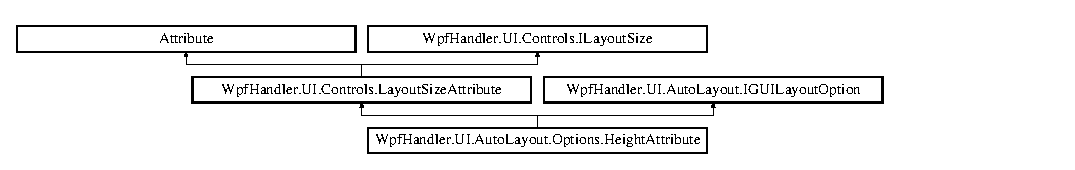
\includegraphics[height=1.842105cm]{d8/d4b/class_wpf_handler_1_1_u_i_1_1_auto_layout_1_1_options_1_1_height_attribute}
\end{center}
\end{figure}
\subsection*{Public Member Functions}
\begin{DoxyCompactItemize}
\item 
\mbox{\hyperlink{class_wpf_handler_1_1_u_i_1_1_auto_layout_1_1_options_1_1_height_attribute_a95fb727e17f5d821370948bfc7ee33a3}{Height\+Attribute}} ()
\begin{DoxyCompactList}\small\item\em Default constructor. Using auto height. \end{DoxyCompactList}\item 
\mbox{\hyperlink{class_wpf_handler_1_1_u_i_1_1_auto_layout_1_1_options_1_1_height_attribute_a96c546720b620ae0b867c25992bad3d6}{Height\+Attribute}} (double height)
\begin{DoxyCompactList}\small\item\em Set requested height as Size. \end{DoxyCompactList}\item 
void \mbox{\hyperlink{class_wpf_handler_1_1_u_i_1_1_auto_layout_1_1_options_1_1_height_attribute_a221d69c339ceb5cd3e16d8e59f216cc9}{Apply\+Layout\+Option}} (Framework\+Element element)
\begin{DoxyCompactList}\small\item\em Define height of the G\+UI element. \end{DoxyCompactList}\end{DoxyCompactItemize}
\subsection*{Additional Inherited Members}


\subsection{Detailed Description}
Define height of the G\+UI element. 



\subsection{Constructor \& Destructor Documentation}
\mbox{\Hypertarget{class_wpf_handler_1_1_u_i_1_1_auto_layout_1_1_options_1_1_height_attribute_a95fb727e17f5d821370948bfc7ee33a3}\label{class_wpf_handler_1_1_u_i_1_1_auto_layout_1_1_options_1_1_height_attribute_a95fb727e17f5d821370948bfc7ee33a3}} 
\index{Wpf\+Handler\+::\+U\+I\+::\+Auto\+Layout\+::\+Options\+::\+Height\+Attribute@{Wpf\+Handler\+::\+U\+I\+::\+Auto\+Layout\+::\+Options\+::\+Height\+Attribute}!Height\+Attribute@{Height\+Attribute}}
\index{Height\+Attribute@{Height\+Attribute}!Wpf\+Handler\+::\+U\+I\+::\+Auto\+Layout\+::\+Options\+::\+Height\+Attribute@{Wpf\+Handler\+::\+U\+I\+::\+Auto\+Layout\+::\+Options\+::\+Height\+Attribute}}
\subsubsection{\texorpdfstring{Height\+Attribute()}{HeightAttribute()}\hspace{0.1cm}{\footnotesize\ttfamily [1/2]}}
{\footnotesize\ttfamily Wpf\+Handler.\+U\+I.\+Auto\+Layout.\+Options.\+Height\+Attribute.\+Height\+Attribute (\begin{DoxyParamCaption}{ }\end{DoxyParamCaption})}



Default constructor. Using auto height. 

\mbox{\Hypertarget{class_wpf_handler_1_1_u_i_1_1_auto_layout_1_1_options_1_1_height_attribute_a96c546720b620ae0b867c25992bad3d6}\label{class_wpf_handler_1_1_u_i_1_1_auto_layout_1_1_options_1_1_height_attribute_a96c546720b620ae0b867c25992bad3d6}} 
\index{Wpf\+Handler\+::\+U\+I\+::\+Auto\+Layout\+::\+Options\+::\+Height\+Attribute@{Wpf\+Handler\+::\+U\+I\+::\+Auto\+Layout\+::\+Options\+::\+Height\+Attribute}!Height\+Attribute@{Height\+Attribute}}
\index{Height\+Attribute@{Height\+Attribute}!Wpf\+Handler\+::\+U\+I\+::\+Auto\+Layout\+::\+Options\+::\+Height\+Attribute@{Wpf\+Handler\+::\+U\+I\+::\+Auto\+Layout\+::\+Options\+::\+Height\+Attribute}}
\subsubsection{\texorpdfstring{Height\+Attribute()}{HeightAttribute()}\hspace{0.1cm}{\footnotesize\ttfamily [2/2]}}
{\footnotesize\ttfamily Wpf\+Handler.\+U\+I.\+Auto\+Layout.\+Options.\+Height\+Attribute.\+Height\+Attribute (\begin{DoxyParamCaption}\item[{double}]{height }\end{DoxyParamCaption})}



Set requested height as Size. 


\begin{DoxyParams}{Parameters}
{\em height} & \\
\hline
\end{DoxyParams}


\subsection{Member Function Documentation}
\mbox{\Hypertarget{class_wpf_handler_1_1_u_i_1_1_auto_layout_1_1_options_1_1_height_attribute_a221d69c339ceb5cd3e16d8e59f216cc9}\label{class_wpf_handler_1_1_u_i_1_1_auto_layout_1_1_options_1_1_height_attribute_a221d69c339ceb5cd3e16d8e59f216cc9}} 
\index{Wpf\+Handler\+::\+U\+I\+::\+Auto\+Layout\+::\+Options\+::\+Height\+Attribute@{Wpf\+Handler\+::\+U\+I\+::\+Auto\+Layout\+::\+Options\+::\+Height\+Attribute}!Apply\+Layout\+Option@{Apply\+Layout\+Option}}
\index{Apply\+Layout\+Option@{Apply\+Layout\+Option}!Wpf\+Handler\+::\+U\+I\+::\+Auto\+Layout\+::\+Options\+::\+Height\+Attribute@{Wpf\+Handler\+::\+U\+I\+::\+Auto\+Layout\+::\+Options\+::\+Height\+Attribute}}
\subsubsection{\texorpdfstring{Apply\+Layout\+Option()}{ApplyLayoutOption()}}
{\footnotesize\ttfamily void Wpf\+Handler.\+U\+I.\+Auto\+Layout.\+Options.\+Height\+Attribute.\+Apply\+Layout\+Option (\begin{DoxyParamCaption}\item[{Framework\+Element}]{element }\end{DoxyParamCaption})}



Define height of the G\+UI element. 


\begin{DoxyParams}{Parameters}
{\em element} & Shared \mbox{\hyperlink{namespace_wpf_handler_1_1_u_i}{UI}} element.\\
\hline
\end{DoxyParams}


Implements \mbox{\hyperlink{interface_wpf_handler_1_1_u_i_1_1_auto_layout_1_1_i_g_u_i_layout_option_ac2d2fa8aeaf753b3248381399f991005}{Wpf\+Handler.\+U\+I.\+Auto\+Layout.\+I\+G\+U\+I\+Layout\+Option}}.



The documentation for this class was generated from the following file\+:\begin{DoxyCompactItemize}
\item 
D\+:/\+Work/\+Git\+Hub/wpf-\/handler/\+Wpf\+Handler/\+U\+I/\+Auto\+Layout/\+Options/Height\+Attribute.\+cs\end{DoxyCompactItemize}

\hypertarget{class_wpf_handler_1_1_u_i_1_1_auto_layout_1_1_configuration_1_1_hide_in_inspector_attribute}{}\section{Wpf\+Handler.\+U\+I.\+Auto\+Layout.\+Configuration.\+Hide\+In\+Inspector\+Attribute Class Reference}
\label{class_wpf_handler_1_1_u_i_1_1_auto_layout_1_1_configuration_1_1_hide_in_inspector_attribute}\index{Wpf\+Handler.\+U\+I.\+Auto\+Layout.\+Configuration.\+Hide\+In\+Inspector\+Attribute@{Wpf\+Handler.\+U\+I.\+Auto\+Layout.\+Configuration.\+Hide\+In\+Inspector\+Attribute}}


Exclude a member from auto-\/builded inspector.  


Inheritance diagram for Wpf\+Handler.\+U\+I.\+Auto\+Layout.\+Configuration.\+Hide\+In\+Inspector\+Attribute\+:\begin{figure}[H]
\begin{center}
\leavevmode
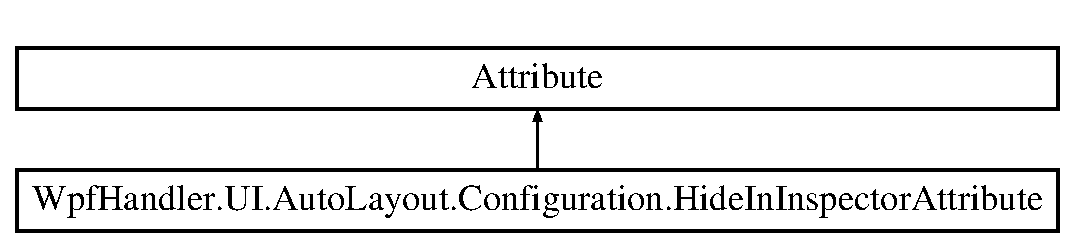
\includegraphics[height=2.000000cm]{d4/d91/class_wpf_handler_1_1_u_i_1_1_auto_layout_1_1_configuration_1_1_hide_in_inspector_attribute}
\end{center}
\end{figure}


\subsection{Detailed Description}
Exclude a member from auto-\/builded inspector. 



The documentation for this class was generated from the following file\+:\begin{DoxyCompactItemize}
\item 
D\+:/\+Work/\+Git\+Hub/wpf-\/handler/\+Wpf\+Handler/\+U\+I/\+Auto\+Layout/\+Configuration/Hide\+In\+Inspector\+Attribute.\+cs\end{DoxyCompactItemize}

\hypertarget{class_wpf_handler_1_1_u_i_1_1_auto_layout_1_1_options_1_1_horizontal_align_attribute}{}\section{Wpf\+Handler.\+U\+I.\+Auto\+Layout.\+Options.\+Horizontal\+Align\+Attribute Class Reference}
\label{class_wpf_handler_1_1_u_i_1_1_auto_layout_1_1_options_1_1_horizontal_align_attribute}\index{Wpf\+Handler.\+U\+I.\+Auto\+Layout.\+Options.\+Horizontal\+Align\+Attribute@{Wpf\+Handler.\+U\+I.\+Auto\+Layout.\+Options.\+Horizontal\+Align\+Attribute}}


Define horizontal align of the G\+UI element.  


Inheritance diagram for Wpf\+Handler.\+U\+I.\+Auto\+Layout.\+Options.\+Horizontal\+Align\+Attribute\+:\begin{figure}[H]
\begin{center}
\leavevmode
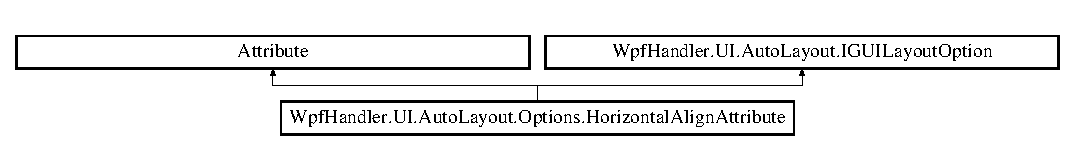
\includegraphics[height=1.581921cm]{da/de4/class_wpf_handler_1_1_u_i_1_1_auto_layout_1_1_options_1_1_horizontal_align_attribute}
\end{center}
\end{figure}
\subsection*{Public Member Functions}
\begin{DoxyCompactItemize}
\item 
void \mbox{\hyperlink{class_wpf_handler_1_1_u_i_1_1_auto_layout_1_1_options_1_1_horizontal_align_attribute_a53335e3d47b8509f6ce67ad93044a760}{Apply\+Layout\+Option}} (Framework\+Element element)
\begin{DoxyCompactList}\small\item\em Define horizontal align of the G\+UI element. \end{DoxyCompactList}\end{DoxyCompactItemize}
\subsection*{Properties}
\begin{DoxyCompactItemize}
\item 
Horizontal\+Alignment \mbox{\hyperlink{class_wpf_handler_1_1_u_i_1_1_auto_layout_1_1_options_1_1_horizontal_align_attribute_a7e62bc68b5e19d0f8167a97146996b6c}{Alignment}}\hspace{0.3cm}{\ttfamily  \mbox{[}get, set\mbox{]}}
\begin{DoxyCompactList}\small\item\em Alignment that will applied to G\+UI element. \end{DoxyCompactList}\end{DoxyCompactItemize}


\subsection{Detailed Description}
Define horizontal align of the G\+UI element. 



\subsection{Member Function Documentation}
\mbox{\Hypertarget{class_wpf_handler_1_1_u_i_1_1_auto_layout_1_1_options_1_1_horizontal_align_attribute_a53335e3d47b8509f6ce67ad93044a760}\label{class_wpf_handler_1_1_u_i_1_1_auto_layout_1_1_options_1_1_horizontal_align_attribute_a53335e3d47b8509f6ce67ad93044a760}} 
\index{Wpf\+Handler\+::\+U\+I\+::\+Auto\+Layout\+::\+Options\+::\+Horizontal\+Align\+Attribute@{Wpf\+Handler\+::\+U\+I\+::\+Auto\+Layout\+::\+Options\+::\+Horizontal\+Align\+Attribute}!Apply\+Layout\+Option@{Apply\+Layout\+Option}}
\index{Apply\+Layout\+Option@{Apply\+Layout\+Option}!Wpf\+Handler\+::\+U\+I\+::\+Auto\+Layout\+::\+Options\+::\+Horizontal\+Align\+Attribute@{Wpf\+Handler\+::\+U\+I\+::\+Auto\+Layout\+::\+Options\+::\+Horizontal\+Align\+Attribute}}
\subsubsection{\texorpdfstring{Apply\+Layout\+Option()}{ApplyLayoutOption()}}
{\footnotesize\ttfamily void Wpf\+Handler.\+U\+I.\+Auto\+Layout.\+Options.\+Horizontal\+Align\+Attribute.\+Apply\+Layout\+Option (\begin{DoxyParamCaption}\item[{Framework\+Element}]{element }\end{DoxyParamCaption})}



Define horizontal align of the G\+UI element. 


\begin{DoxyParams}{Parameters}
{\em element} & Shared \mbox{\hyperlink{namespace_wpf_handler_1_1_u_i}{UI}} element.\\
\hline
\end{DoxyParams}


Implements \mbox{\hyperlink{interface_wpf_handler_1_1_u_i_1_1_auto_layout_1_1_i_g_u_i_layout_option_ac2d2fa8aeaf753b3248381399f991005}{Wpf\+Handler.\+U\+I.\+Auto\+Layout.\+I\+G\+U\+I\+Layout\+Option}}.



\subsection{Property Documentation}
\mbox{\Hypertarget{class_wpf_handler_1_1_u_i_1_1_auto_layout_1_1_options_1_1_horizontal_align_attribute_a7e62bc68b5e19d0f8167a97146996b6c}\label{class_wpf_handler_1_1_u_i_1_1_auto_layout_1_1_options_1_1_horizontal_align_attribute_a7e62bc68b5e19d0f8167a97146996b6c}} 
\index{Wpf\+Handler\+::\+U\+I\+::\+Auto\+Layout\+::\+Options\+::\+Horizontal\+Align\+Attribute@{Wpf\+Handler\+::\+U\+I\+::\+Auto\+Layout\+::\+Options\+::\+Horizontal\+Align\+Attribute}!Alignment@{Alignment}}
\index{Alignment@{Alignment}!Wpf\+Handler\+::\+U\+I\+::\+Auto\+Layout\+::\+Options\+::\+Horizontal\+Align\+Attribute@{Wpf\+Handler\+::\+U\+I\+::\+Auto\+Layout\+::\+Options\+::\+Horizontal\+Align\+Attribute}}
\subsubsection{\texorpdfstring{Alignment}{Alignment}}
{\footnotesize\ttfamily Horizontal\+Alignment Wpf\+Handler.\+U\+I.\+Auto\+Layout.\+Options.\+Horizontal\+Align\+Attribute.\+Alignment\hspace{0.3cm}{\ttfamily [get]}, {\ttfamily [set]}}



Alignment that will applied to G\+UI element. 



The documentation for this class was generated from the following file\+:\begin{DoxyCompactItemize}
\item 
D\+:/\+Work/\+Git\+Hub/wpf-\/handler/\+Wpf\+Handler/\+U\+I/\+Auto\+Layout/\+Options/Horizontal\+Align\+Attribute.\+cs\end{DoxyCompactItemize}

\hypertarget{interface_wpf_handler_1_1_u_i_1_1_auto_layout_1_1_i_g_u_i_element}{}\section{Wpf\+Handler.\+U\+I.\+Auto\+Layout.\+I\+G\+U\+I\+Element Interface Reference}
\label{interface_wpf_handler_1_1_u_i_1_1_auto_layout_1_1_i_g_u_i_element}\index{Wpf\+Handler.\+U\+I.\+Auto\+Layout.\+I\+G\+U\+I\+Element@{Wpf\+Handler.\+U\+I.\+Auto\+Layout.\+I\+G\+U\+I\+Element}}


Implementing of that interface allow to modify current layout during calling.  


Inheritance diagram for Wpf\+Handler.\+U\+I.\+Auto\+Layout.\+I\+G\+U\+I\+Element\+:\begin{figure}[H]
\begin{center}
\leavevmode
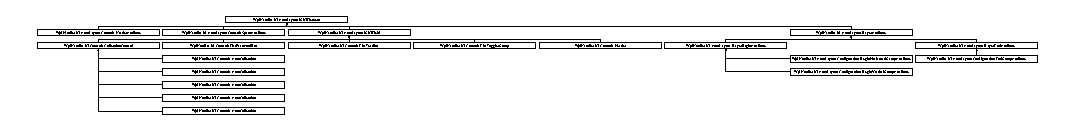
\includegraphics[height=1.171242cm]{da/db2/interface_wpf_handler_1_1_u_i_1_1_auto_layout_1_1_i_g_u_i_element}
\end{center}
\end{figure}
\subsection*{Public Member Functions}
\begin{DoxyCompactItemize}
\item 
void \mbox{\hyperlink{interface_wpf_handler_1_1_u_i_1_1_auto_layout_1_1_i_g_u_i_element_a0ff16956f8e8187d51e1b36b6b9f894e}{On\+Layout}} (ref \mbox{\hyperlink{class_wpf_handler_1_1_u_i_1_1_auto_layout_1_1_layout_layer}{Layout\+Layer}} layer, params object\mbox{[}$\,$\mbox{]} args)
\begin{DoxyCompactList}\small\item\em Modify current layer\textquotesingle{}s layout according to G\+UI element requirments. Calls once during \mbox{\hyperlink{namespace_wpf_handler_1_1_u_i}{UI}} spawn. \end{DoxyCompactList}\end{DoxyCompactItemize}


\subsection{Detailed Description}
Implementing of that interface allow to modify current layout during calling. 



\subsection{Member Function Documentation}
\mbox{\Hypertarget{interface_wpf_handler_1_1_u_i_1_1_auto_layout_1_1_i_g_u_i_element_a0ff16956f8e8187d51e1b36b6b9f894e}\label{interface_wpf_handler_1_1_u_i_1_1_auto_layout_1_1_i_g_u_i_element_a0ff16956f8e8187d51e1b36b6b9f894e}} 
\index{Wpf\+Handler\+::\+U\+I\+::\+Auto\+Layout\+::\+I\+G\+U\+I\+Element@{Wpf\+Handler\+::\+U\+I\+::\+Auto\+Layout\+::\+I\+G\+U\+I\+Element}!On\+Layout@{On\+Layout}}
\index{On\+Layout@{On\+Layout}!Wpf\+Handler\+::\+U\+I\+::\+Auto\+Layout\+::\+I\+G\+U\+I\+Element@{Wpf\+Handler\+::\+U\+I\+::\+Auto\+Layout\+::\+I\+G\+U\+I\+Element}}
\subsubsection{\texorpdfstring{On\+Layout()}{OnLayout()}}
{\footnotesize\ttfamily void Wpf\+Handler.\+U\+I.\+Auto\+Layout.\+I\+G\+U\+I\+Element.\+On\+Layout (\begin{DoxyParamCaption}\item[{ref \mbox{\hyperlink{class_wpf_handler_1_1_u_i_1_1_auto_layout_1_1_layout_layer}{Layout\+Layer}}}]{layer,  }\item[{params object \mbox{[}$\,$\mbox{]}}]{args }\end{DoxyParamCaption})}



Modify current layer\textquotesingle{}s layout according to G\+UI element requirments. Calls once during \mbox{\hyperlink{namespace_wpf_handler_1_1_u_i}{UI}} spawn. 


\begin{DoxyParams}{Parameters}
{\em layer} & Target G\+UI layer.\\
\hline
{\em args} & Shared arguments.\\
\hline
\end{DoxyParams}


Implemented in \mbox{\hyperlink{class_wpf_handler_1_1_u_i_1_1_controls_1_1_collection_control_a54cf416fee122e600059ed8713d75bb0}{Wpf\+Handler.\+U\+I.\+Controls.\+Collection\+Control}}, \mbox{\hyperlink{class_wpf_handler_1_1_u_i_1_1_controls_1_1_flat_toggles_group_a5619e5107d6cbc3fb2cdabb21deb40a4}{Wpf\+Handler.\+U\+I.\+Controls.\+Flat\+Toggles\+Group}}, \mbox{\hyperlink{class_wpf_handler_1_1_u_i_1_1_controls_1_1_header_a23ac86ea123581ee90d1aa9b6a81dadd}{Wpf\+Handler.\+U\+I.\+Controls.\+Header}}, \mbox{\hyperlink{class_wpf_handler_1_1_u_i_1_1_controls_1_1_flat_password_box_a8a06600a127d2b9bc7a1a04767f383e8}{Wpf\+Handler.\+U\+I.\+Controls.\+Flat\+Password\+Box}}, \mbox{\hyperlink{class_wpf_handler_1_1_u_i_1_1_controls_1_1_flat_text_box_a9885e81c438caeec3448c99796503a71}{Wpf\+Handler.\+U\+I.\+Controls.\+Flat\+Text\+Box}}, \mbox{\hyperlink{class_wpf_handler_1_1_u_i_1_1_auto_layout_1_1_controls_1_1_header_attribute_a837805f9b975447e7cf5663119189c37}{Wpf\+Handler.\+U\+I.\+Auto\+Layout.\+Controls.\+Header\+Attribute}}, \mbox{\hyperlink{class_wpf_handler_1_1_u_i_1_1_auto_layout_1_1_controls_1_1_label_attribute_a70b5b79babc0fd60171ba08231ce2a5c}{Wpf\+Handler.\+U\+I.\+Auto\+Layout.\+Controls.\+Label\+Attribute}}, \mbox{\hyperlink{class_wpf_handler_1_1_u_i_1_1_auto_layout_1_1_controls_1_1_space_attribute_abc4dedcaa52529fb4f0e227fb2386866}{Wpf\+Handler.\+U\+I.\+Auto\+Layout.\+Controls.\+Space\+Attribute}}, \mbox{\hyperlink{class_wpf_handler_1_1_u_i_1_1_auto_layout_1_1_configuration_1_1_begin_horizontal_group_attribute_a8bb61f969389bece86c87fbfa44d4c82}{Wpf\+Handler.\+U\+I.\+Auto\+Layout.\+Configuration.\+Begin\+Horizontal\+Group\+Attribute}}, \mbox{\hyperlink{class_wpf_handler_1_1_u_i_1_1_auto_layout_1_1_configuration_1_1_begin_vertical_group_attribute_a52859bc4d83f107cbae35d20ae97ce83}{Wpf\+Handler.\+U\+I.\+Auto\+Layout.\+Configuration.\+Begin\+Vertical\+Group\+Attribute}}, and \mbox{\hyperlink{class_wpf_handler_1_1_u_i_1_1_auto_layout_1_1_configuration_1_1_end_group_attribute_acaed685d0daf2b14d8f232389d56c478}{Wpf\+Handler.\+U\+I.\+Auto\+Layout.\+Configuration.\+End\+Group\+Attribute}}.



The documentation for this interface was generated from the following file\+:\begin{DoxyCompactItemize}
\item 
D\+:/\+Work/\+Git\+Hub/wpf-\/handler/\+Wpf\+Handler/\+U\+I/\+Auto\+Layout/\+Interfaces/I\+G\+U\+I\+Element.\+cs\end{DoxyCompactItemize}

\hypertarget{interface_wpf_handler_1_1_u_i_1_1_auto_layout_1_1_markups_1_1_i_g_u_i_element_binding_attribute}{}\section{Wpf\+Handler.\+U\+I.\+Auto\+Layout.\+Markups.\+I\+G\+U\+I\+Element\+Binding\+Attribute Interface Reference}
\label{interface_wpf_handler_1_1_u_i_1_1_auto_layout_1_1_markups_1_1_i_g_u_i_element_binding_attribute}\index{Wpf\+Handler.\+U\+I.\+Auto\+Layout.\+Markups.\+I\+G\+U\+I\+Element\+Binding\+Attribute@{Wpf\+Handler.\+U\+I.\+Auto\+Layout.\+Markups.\+I\+G\+U\+I\+Element\+Binding\+Attribute}}


Implementation of that interface marks the attribute as the one who using into specifying of a G\+UI element binding process.  


Inheritance diagram for Wpf\+Handler.\+U\+I.\+Auto\+Layout.\+Markups.\+I\+G\+U\+I\+Element\+Binding\+Attribute\+:\begin{figure}[H]
\begin{center}
\leavevmode
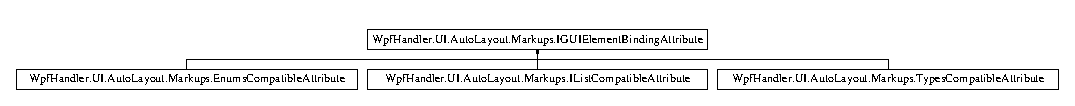
\includegraphics[height=0.974761cm]{d4/d32/interface_wpf_handler_1_1_u_i_1_1_auto_layout_1_1_markups_1_1_i_g_u_i_element_binding_attribute}
\end{center}
\end{figure}


\subsection{Detailed Description}
Implementation of that interface marks the attribute as the one who using into specifying of a G\+UI element binding process. 



The documentation for this interface was generated from the following file\+:\begin{DoxyCompactItemize}
\item 
D\+:/\+Work/\+Git\+Hub/wpf-\/handler/\+Wpf\+Handler/\+U\+I/\+Auto\+Layout/\+Markups/I\+G\+U\+I\+Element\+Binding\+Attribute.\+cs\end{DoxyCompactItemize}

\hypertarget{interface_wpf_handler_1_1_u_i_1_1_auto_layout_1_1_i_g_u_i_field}{}\section{Wpf\+Handler.\+U\+I.\+Auto\+Layout.\+I\+G\+U\+I\+Field Interface Reference}
\label{interface_wpf_handler_1_1_u_i_1_1_auto_layout_1_1_i_g_u_i_field}\index{Wpf\+Handler.\+U\+I.\+Auto\+Layout.\+I\+G\+U\+I\+Field@{Wpf\+Handler.\+U\+I.\+Auto\+Layout.\+I\+G\+U\+I\+Field}}


Implementation of that interface allow to use that control in auto layout user interfaces.  


Inheritance diagram for Wpf\+Handler.\+U\+I.\+Auto\+Layout.\+I\+G\+U\+I\+Field\+:\begin{figure}[H]
\begin{center}
\leavevmode
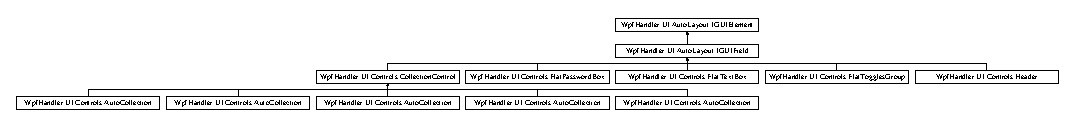
\includegraphics[height=1.245136cm]{d3/dac/interface_wpf_handler_1_1_u_i_1_1_auto_layout_1_1_i_g_u_i_field}
\end{center}
\end{figure}
\subsection*{Properties}
\begin{DoxyCompactItemize}
\item 
object \mbox{\hyperlink{interface_wpf_handler_1_1_u_i_1_1_auto_layout_1_1_i_g_u_i_field_a6603f5bb3eeee52e2d061d6d0f40720a}{Value}}\hspace{0.3cm}{\ttfamily  \mbox{[}get, set\mbox{]}}
\begin{DoxyCompactList}\small\item\em Value of that control. \end{DoxyCompactList}\item 
Member\+Info \mbox{\hyperlink{interface_wpf_handler_1_1_u_i_1_1_auto_layout_1_1_i_g_u_i_field_a063a35928be8b8f839f560d3c8af33e7}{Binded\+Member}}\hspace{0.3cm}{\ttfamily  \mbox{[}get, set\mbox{]}}
\begin{DoxyCompactList}\small\item\em Memeber that will be used as source for the value into \mbox{\hyperlink{namespace_wpf_handler_1_1_u_i}{UI}}. \end{DoxyCompactList}\end{DoxyCompactItemize}
\subsection*{Events}
\begin{DoxyCompactItemize}
\item 
System.\+Action$<$ \mbox{\hyperlink{interface_wpf_handler_1_1_u_i_1_1_auto_layout_1_1_i_g_u_i_field}{I\+G\+U\+I\+Field}} $>$ \mbox{\hyperlink{interface_wpf_handler_1_1_u_i_1_1_auto_layout_1_1_i_g_u_i_field_a97d9c046f0ed12e42560f2c7fb414d5f}{Value\+Changed}}
\begin{DoxyCompactList}\small\item\em Event that will occure in case if value of the field will be changed. Will cause updating of the Binded\+Member value. \end{DoxyCompactList}\end{DoxyCompactItemize}
\subsection*{Additional Inherited Members}


\subsection{Detailed Description}
Implementation of that interface allow to use that control in auto layout user interfaces. 



\subsection{Property Documentation}
\mbox{\Hypertarget{interface_wpf_handler_1_1_u_i_1_1_auto_layout_1_1_i_g_u_i_field_a063a35928be8b8f839f560d3c8af33e7}\label{interface_wpf_handler_1_1_u_i_1_1_auto_layout_1_1_i_g_u_i_field_a063a35928be8b8f839f560d3c8af33e7}} 
\index{Wpf\+Handler\+::\+U\+I\+::\+Auto\+Layout\+::\+I\+G\+U\+I\+Field@{Wpf\+Handler\+::\+U\+I\+::\+Auto\+Layout\+::\+I\+G\+U\+I\+Field}!Binded\+Member@{Binded\+Member}}
\index{Binded\+Member@{Binded\+Member}!Wpf\+Handler\+::\+U\+I\+::\+Auto\+Layout\+::\+I\+G\+U\+I\+Field@{Wpf\+Handler\+::\+U\+I\+::\+Auto\+Layout\+::\+I\+G\+U\+I\+Field}}
\subsubsection{\texorpdfstring{Binded\+Member}{BindedMember}}
{\footnotesize\ttfamily Member\+Info Wpf\+Handler.\+U\+I.\+Auto\+Layout.\+I\+G\+U\+I\+Field.\+Binded\+Member\hspace{0.3cm}{\ttfamily [get]}, {\ttfamily [set]}}



Memeber that will be used as source for the value into \mbox{\hyperlink{namespace_wpf_handler_1_1_u_i}{UI}}. 

\mbox{\Hypertarget{interface_wpf_handler_1_1_u_i_1_1_auto_layout_1_1_i_g_u_i_field_a6603f5bb3eeee52e2d061d6d0f40720a}\label{interface_wpf_handler_1_1_u_i_1_1_auto_layout_1_1_i_g_u_i_field_a6603f5bb3eeee52e2d061d6d0f40720a}} 
\index{Wpf\+Handler\+::\+U\+I\+::\+Auto\+Layout\+::\+I\+G\+U\+I\+Field@{Wpf\+Handler\+::\+U\+I\+::\+Auto\+Layout\+::\+I\+G\+U\+I\+Field}!Value@{Value}}
\index{Value@{Value}!Wpf\+Handler\+::\+U\+I\+::\+Auto\+Layout\+::\+I\+G\+U\+I\+Field@{Wpf\+Handler\+::\+U\+I\+::\+Auto\+Layout\+::\+I\+G\+U\+I\+Field}}
\subsubsection{\texorpdfstring{Value}{Value}}
{\footnotesize\ttfamily object Wpf\+Handler.\+U\+I.\+Auto\+Layout.\+I\+G\+U\+I\+Field.\+Value\hspace{0.3cm}{\ttfamily [get]}, {\ttfamily [set]}}



Value of that control. 



\subsection{Event Documentation}
\mbox{\Hypertarget{interface_wpf_handler_1_1_u_i_1_1_auto_layout_1_1_i_g_u_i_field_a97d9c046f0ed12e42560f2c7fb414d5f}\label{interface_wpf_handler_1_1_u_i_1_1_auto_layout_1_1_i_g_u_i_field_a97d9c046f0ed12e42560f2c7fb414d5f}} 
\index{Wpf\+Handler\+::\+U\+I\+::\+Auto\+Layout\+::\+I\+G\+U\+I\+Field@{Wpf\+Handler\+::\+U\+I\+::\+Auto\+Layout\+::\+I\+G\+U\+I\+Field}!Value\+Changed@{Value\+Changed}}
\index{Value\+Changed@{Value\+Changed}!Wpf\+Handler\+::\+U\+I\+::\+Auto\+Layout\+::\+I\+G\+U\+I\+Field@{Wpf\+Handler\+::\+U\+I\+::\+Auto\+Layout\+::\+I\+G\+U\+I\+Field}}
\subsubsection{\texorpdfstring{Value\+Changed}{ValueChanged}}
{\footnotesize\ttfamily System.\+Action$<$\mbox{\hyperlink{interface_wpf_handler_1_1_u_i_1_1_auto_layout_1_1_i_g_u_i_field}{I\+G\+U\+I\+Field}}$>$ Wpf\+Handler.\+U\+I.\+Auto\+Layout.\+I\+G\+U\+I\+Field.\+Value\+Changed}



Event that will occure in case if value of the field will be changed. Will cause updating of the Binded\+Member value. 

\mbox{\hyperlink{interface_wpf_handler_1_1_u_i_1_1_auto_layout_1_1_i_g_u_i_field}{I\+G\+U\+I\+Field}} -\/ sender. 

The documentation for this interface was generated from the following file\+:\begin{DoxyCompactItemize}
\item 
D\+:/\+Work/\+Git\+Hub/wpf-\/handler/\+Wpf\+Handler/\+U\+I/\+Auto\+Layout/\+Interfaces/I\+G\+U\+I\+Field.\+cs\end{DoxyCompactItemize}

\hypertarget{interface_wpf_handler_1_1_u_i_1_1_auto_layout_1_1_i_g_u_i_layout_option}{}\section{Wpf\+Handler.\+U\+I.\+Auto\+Layout.\+I\+G\+U\+I\+Layout\+Option Interface Reference}
\label{interface_wpf_handler_1_1_u_i_1_1_auto_layout_1_1_i_g_u_i_layout_option}\index{Wpf\+Handler.\+U\+I.\+Auto\+Layout.\+I\+G\+U\+I\+Layout\+Option@{Wpf\+Handler.\+U\+I.\+Auto\+Layout.\+I\+G\+U\+I\+Layout\+Option}}


Interface that implement custom layout options performing.  


Inheritance diagram for Wpf\+Handler.\+U\+I.\+Auto\+Layout.\+I\+G\+U\+I\+Layout\+Option\+:\begin{figure}[H]
\begin{center}
\leavevmode
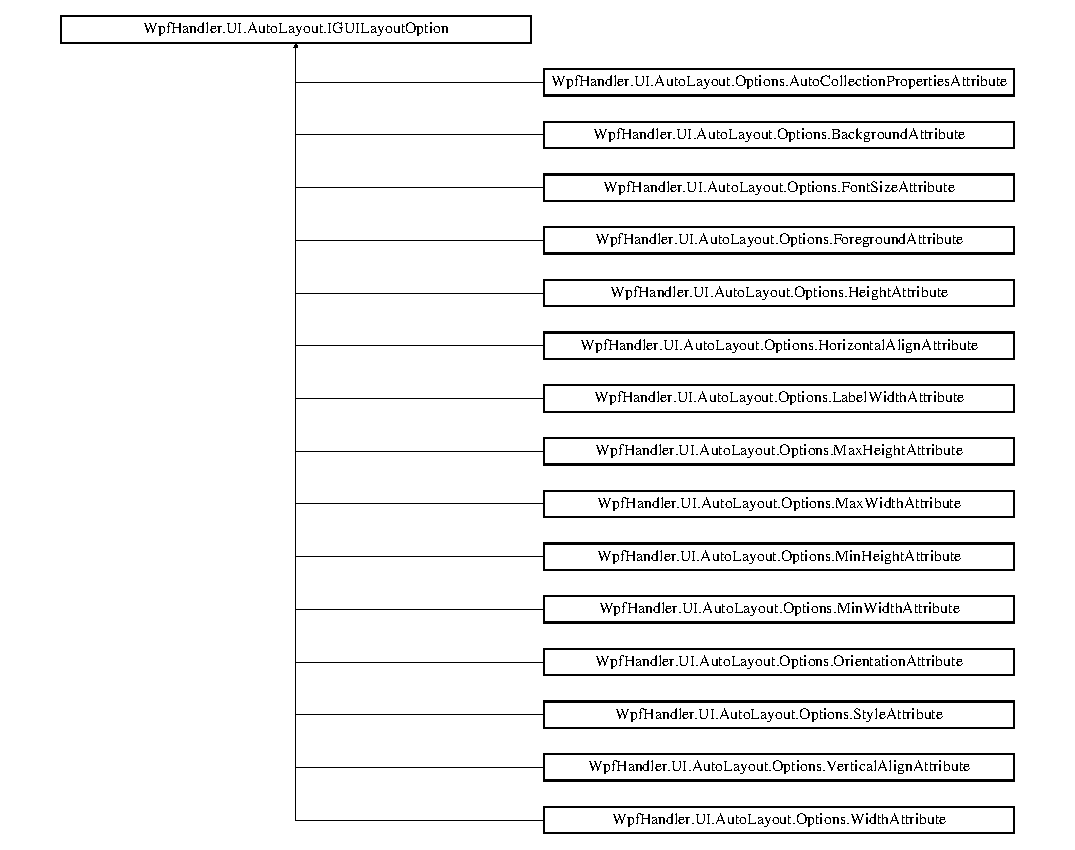
\includegraphics[height=10.980392cm]{d0/dfe/interface_wpf_handler_1_1_u_i_1_1_auto_layout_1_1_i_g_u_i_layout_option}
\end{center}
\end{figure}
\subsection*{Public Member Functions}
\begin{DoxyCompactItemize}
\item 
void \mbox{\hyperlink{interface_wpf_handler_1_1_u_i_1_1_auto_layout_1_1_i_g_u_i_layout_option_ac2d2fa8aeaf753b3248381399f991005}{Apply\+Layout\+Option}} (Framework\+Element element)
\begin{DoxyCompactList}\small\item\em Aplying option to the element. \end{DoxyCompactList}\end{DoxyCompactItemize}


\subsection{Detailed Description}
Interface that implement custom layout options performing. 



\subsection{Member Function Documentation}
\mbox{\Hypertarget{interface_wpf_handler_1_1_u_i_1_1_auto_layout_1_1_i_g_u_i_layout_option_ac2d2fa8aeaf753b3248381399f991005}\label{interface_wpf_handler_1_1_u_i_1_1_auto_layout_1_1_i_g_u_i_layout_option_ac2d2fa8aeaf753b3248381399f991005}} 
\index{Wpf\+Handler\+::\+U\+I\+::\+Auto\+Layout\+::\+I\+G\+U\+I\+Layout\+Option@{Wpf\+Handler\+::\+U\+I\+::\+Auto\+Layout\+::\+I\+G\+U\+I\+Layout\+Option}!Apply\+Layout\+Option@{Apply\+Layout\+Option}}
\index{Apply\+Layout\+Option@{Apply\+Layout\+Option}!Wpf\+Handler\+::\+U\+I\+::\+Auto\+Layout\+::\+I\+G\+U\+I\+Layout\+Option@{Wpf\+Handler\+::\+U\+I\+::\+Auto\+Layout\+::\+I\+G\+U\+I\+Layout\+Option}}
\subsubsection{\texorpdfstring{Apply\+Layout\+Option()}{ApplyLayoutOption()}}
{\footnotesize\ttfamily void Wpf\+Handler.\+U\+I.\+Auto\+Layout.\+I\+G\+U\+I\+Layout\+Option.\+Apply\+Layout\+Option (\begin{DoxyParamCaption}\item[{Framework\+Element}]{element }\end{DoxyParamCaption})}



Aplying option to the element. 


\begin{DoxyParams}{Parameters}
{\em element} & Target G\+UI element.\\
\hline
\end{DoxyParams}


Implemented in \mbox{\hyperlink{class_wpf_handler_1_1_u_i_1_1_auto_layout_1_1_options_1_1_auto_collection_properties_attribute_aaff2195c793c7e75ac553291d9189655}{Wpf\+Handler.\+U\+I.\+Auto\+Layout.\+Options.\+Auto\+Collection\+Properties\+Attribute}}, \mbox{\hyperlink{class_wpf_handler_1_1_u_i_1_1_auto_layout_1_1_options_1_1_background_attribute_a97cce29c9e19d9145e881c69e3bf3d4e}{Wpf\+Handler.\+U\+I.\+Auto\+Layout.\+Options.\+Background\+Attribute}}, \mbox{\hyperlink{class_wpf_handler_1_1_u_i_1_1_auto_layout_1_1_options_1_1_foreground_attribute_a5231ed2afb4d2d26eac9eab670adca45}{Wpf\+Handler.\+U\+I.\+Auto\+Layout.\+Options.\+Foreground\+Attribute}}, \mbox{\hyperlink{class_wpf_handler_1_1_u_i_1_1_auto_layout_1_1_options_1_1_label_width_attribute_ab8dae5f847875d310747599429c5054a}{Wpf\+Handler.\+U\+I.\+Auto\+Layout.\+Options.\+Label\+Width\+Attribute}}, \mbox{\hyperlink{class_wpf_handler_1_1_u_i_1_1_auto_layout_1_1_options_1_1_height_attribute_a221d69c339ceb5cd3e16d8e59f216cc9}{Wpf\+Handler.\+U\+I.\+Auto\+Layout.\+Options.\+Height\+Attribute}}, \mbox{\hyperlink{class_wpf_handler_1_1_u_i_1_1_auto_layout_1_1_options_1_1_max_height_attribute_a1b1d850c2c5d8e59454d7f9b5271ee88}{Wpf\+Handler.\+U\+I.\+Auto\+Layout.\+Options.\+Max\+Height\+Attribute}}, \mbox{\hyperlink{class_wpf_handler_1_1_u_i_1_1_auto_layout_1_1_options_1_1_max_width_attribute_ab7c7bf52114b1aa465f70debaeccf5f4}{Wpf\+Handler.\+U\+I.\+Auto\+Layout.\+Options.\+Max\+Width\+Attribute}}, \mbox{\hyperlink{class_wpf_handler_1_1_u_i_1_1_auto_layout_1_1_options_1_1_min_height_attribute_a8c049220211484fea64fbd1589a4cc57}{Wpf\+Handler.\+U\+I.\+Auto\+Layout.\+Options.\+Min\+Height\+Attribute}}, \mbox{\hyperlink{class_wpf_handler_1_1_u_i_1_1_auto_layout_1_1_options_1_1_min_width_attribute_a22bf72913c8d5d9f958d1edb1b52beda}{Wpf\+Handler.\+U\+I.\+Auto\+Layout.\+Options.\+Min\+Width\+Attribute}}, \mbox{\hyperlink{class_wpf_handler_1_1_u_i_1_1_auto_layout_1_1_options_1_1_width_attribute_afdff5891e40ae82fc6282d78753ff644}{Wpf\+Handler.\+U\+I.\+Auto\+Layout.\+Options.\+Width\+Attribute}}, \mbox{\hyperlink{class_wpf_handler_1_1_u_i_1_1_auto_layout_1_1_options_1_1_orientation_attribute_affc825395d69d510dfc17e37d330dfc8}{Wpf\+Handler.\+U\+I.\+Auto\+Layout.\+Options.\+Orientation\+Attribute}}, \mbox{\hyperlink{class_wpf_handler_1_1_u_i_1_1_auto_layout_1_1_options_1_1_font_size_attribute_abd93e70e5419e81c4dfdd9b5d1f35343}{Wpf\+Handler.\+U\+I.\+Auto\+Layout.\+Options.\+Font\+Size\+Attribute}}, \mbox{\hyperlink{class_wpf_handler_1_1_u_i_1_1_auto_layout_1_1_options_1_1_horizontal_align_attribute_a53335e3d47b8509f6ce67ad93044a760}{Wpf\+Handler.\+U\+I.\+Auto\+Layout.\+Options.\+Horizontal\+Align\+Attribute}}, \mbox{\hyperlink{class_wpf_handler_1_1_u_i_1_1_auto_layout_1_1_options_1_1_vertical_align_attribute_a5a37e0bcf32b49da94e4f4d539fe810c}{Wpf\+Handler.\+U\+I.\+Auto\+Layout.\+Options.\+Vertical\+Align\+Attribute}}, and \mbox{\hyperlink{class_wpf_handler_1_1_u_i_1_1_auto_layout_1_1_options_1_1_style_attribute_a4507ba7b9729b527b0c4f57bffaac0be}{Wpf\+Handler.\+U\+I.\+Auto\+Layout.\+Options.\+Style\+Attribute}}.



The documentation for this interface was generated from the following file\+:\begin{DoxyCompactItemize}
\item 
D\+:/\+Work/\+Git\+Hub/wpf-\/handler/\+Wpf\+Handler/\+U\+I/\+Auto\+Layout/\+Interfaces/I\+G\+U\+I\+Layout\+Option.\+cs\end{DoxyCompactItemize}

\hypertarget{interface_wpf_handler_1_1_u_i_1_1_controls_1_1_i_label}{}\section{Wpf\+Handler.\+U\+I.\+Controls.\+I\+Label Interface Reference}
\label{interface_wpf_handler_1_1_u_i_1_1_controls_1_1_i_label}\index{Wpf\+Handler.\+U\+I.\+Controls.\+I\+Label@{Wpf\+Handler.\+U\+I.\+Controls.\+I\+Label}}


Implement that interface for controls with existed text label.  


Inheritance diagram for Wpf\+Handler.\+U\+I.\+Controls.\+I\+Label\+:\begin{figure}[H]
\begin{center}
\leavevmode
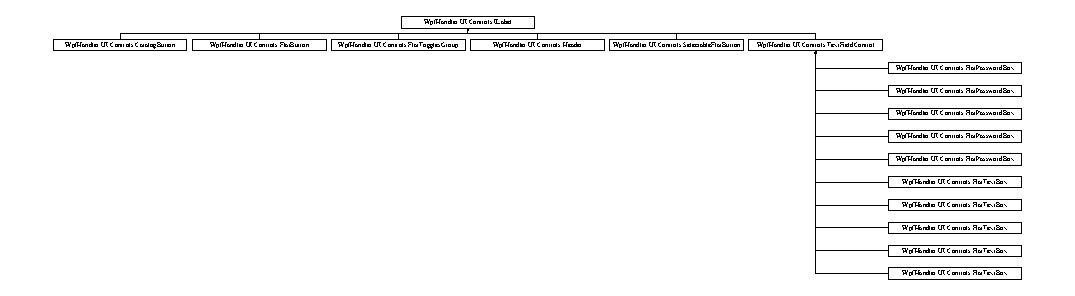
\includegraphics[height=3.529412cm]{dd/de2/interface_wpf_handler_1_1_u_i_1_1_controls_1_1_i_label}
\end{center}
\end{figure}
\subsection*{Properties}
\begin{DoxyCompactItemize}
\item 
string \mbox{\hyperlink{interface_wpf_handler_1_1_u_i_1_1_controls_1_1_i_label_aebbb23ec8dfeb78718107bc877f39c98}{Label}}\hspace{0.3cm}{\ttfamily  \mbox{[}get, set\mbox{]}}
\begin{DoxyCompactList}\small\item\em Text of the label. \end{DoxyCompactList}\item 
float \mbox{\hyperlink{interface_wpf_handler_1_1_u_i_1_1_controls_1_1_i_label_a20f588e0463f8b77531f342415f2eaa4}{Label\+Width}}\hspace{0.3cm}{\ttfamily  \mbox{[}get, set\mbox{]}}
\begin{DoxyCompactList}\small\item\em Width of label field. \end{DoxyCompactList}\end{DoxyCompactItemize}


\subsection{Detailed Description}
Implement that interface for controls with existed text label. 



\subsection{Property Documentation}
\mbox{\Hypertarget{interface_wpf_handler_1_1_u_i_1_1_controls_1_1_i_label_aebbb23ec8dfeb78718107bc877f39c98}\label{interface_wpf_handler_1_1_u_i_1_1_controls_1_1_i_label_aebbb23ec8dfeb78718107bc877f39c98}} 
\index{Wpf\+Handler\+::\+U\+I\+::\+Controls\+::\+I\+Label@{Wpf\+Handler\+::\+U\+I\+::\+Controls\+::\+I\+Label}!Label@{Label}}
\index{Label@{Label}!Wpf\+Handler\+::\+U\+I\+::\+Controls\+::\+I\+Label@{Wpf\+Handler\+::\+U\+I\+::\+Controls\+::\+I\+Label}}
\subsubsection{\texorpdfstring{Label}{Label}}
{\footnotesize\ttfamily string Wpf\+Handler.\+U\+I.\+Controls.\+I\+Label.\+Label\hspace{0.3cm}{\ttfamily [get]}, {\ttfamily [set]}}



Text of the label. 

\mbox{\Hypertarget{interface_wpf_handler_1_1_u_i_1_1_controls_1_1_i_label_a20f588e0463f8b77531f342415f2eaa4}\label{interface_wpf_handler_1_1_u_i_1_1_controls_1_1_i_label_a20f588e0463f8b77531f342415f2eaa4}} 
\index{Wpf\+Handler\+::\+U\+I\+::\+Controls\+::\+I\+Label@{Wpf\+Handler\+::\+U\+I\+::\+Controls\+::\+I\+Label}!Label\+Width@{Label\+Width}}
\index{Label\+Width@{Label\+Width}!Wpf\+Handler\+::\+U\+I\+::\+Controls\+::\+I\+Label@{Wpf\+Handler\+::\+U\+I\+::\+Controls\+::\+I\+Label}}
\subsubsection{\texorpdfstring{Label\+Width}{LabelWidth}}
{\footnotesize\ttfamily float Wpf\+Handler.\+U\+I.\+Controls.\+I\+Label.\+Label\+Width\hspace{0.3cm}{\ttfamily [get]}, {\ttfamily [set]}}



Width of label field. 



The documentation for this interface was generated from the following file\+:\begin{DoxyCompactItemize}
\item 
D\+:/\+Work/\+Git\+Hub/wpf-\/handler/\+Wpf\+Handler/\+U\+I/\+Controls/I\+Label.\+cs\end{DoxyCompactItemize}

\hypertarget{interface_wpf_handler_1_1_u_i_1_1_auto_layout_1_1_i_layer_attribute}{}\section{Wpf\+Handler.\+U\+I.\+Auto\+Layout.\+I\+Layer\+Attribute Interface Reference}
\label{interface_wpf_handler_1_1_u_i_1_1_auto_layout_1_1_i_layer_attribute}\index{Wpf\+Handler.\+U\+I.\+Auto\+Layout.\+I\+Layer\+Attribute@{Wpf\+Handler.\+U\+I.\+Auto\+Layout.\+I\+Layer\+Attribute}}


Define attribute like one that operate with layout layers.  


Inheritance diagram for Wpf\+Handler.\+U\+I.\+Auto\+Layout.\+I\+Layer\+Attribute\+:\begin{figure}[H]
\begin{center}
\leavevmode
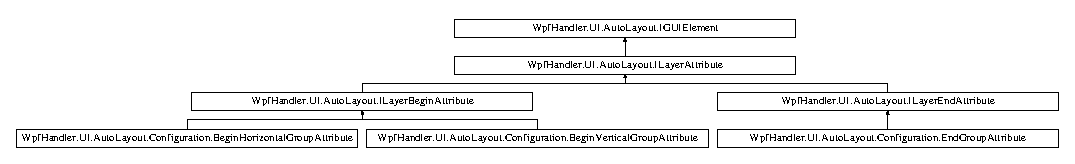
\includegraphics[height=1.756863cm]{d7/d70/interface_wpf_handler_1_1_u_i_1_1_auto_layout_1_1_i_layer_attribute}
\end{center}
\end{figure}
\subsection*{Properties}
\begin{DoxyCompactItemize}
\item 
\mbox{\hyperlink{class_wpf_handler_1_1_u_i_1_1_auto_layout_1_1_layout_layer}{Layout\+Layer}} \mbox{\hyperlink{interface_wpf_handler_1_1_u_i_1_1_auto_layout_1_1_i_layer_attribute_a0af8e554e80237be99bf7927749ff49f}{Layer}}\hspace{0.3cm}{\ttfamily  \mbox{[}get\mbox{]}}
\begin{DoxyCompactList}\small\item\em Layer that opereted into the handler. \end{DoxyCompactList}\end{DoxyCompactItemize}
\subsection*{Additional Inherited Members}


\subsection{Detailed Description}
Define attribute like one that operate with layout layers. 



\subsection{Property Documentation}
\mbox{\Hypertarget{interface_wpf_handler_1_1_u_i_1_1_auto_layout_1_1_i_layer_attribute_a0af8e554e80237be99bf7927749ff49f}\label{interface_wpf_handler_1_1_u_i_1_1_auto_layout_1_1_i_layer_attribute_a0af8e554e80237be99bf7927749ff49f}} 
\index{Wpf\+Handler\+::\+U\+I\+::\+Auto\+Layout\+::\+I\+Layer\+Attribute@{Wpf\+Handler\+::\+U\+I\+::\+Auto\+Layout\+::\+I\+Layer\+Attribute}!Layer@{Layer}}
\index{Layer@{Layer}!Wpf\+Handler\+::\+U\+I\+::\+Auto\+Layout\+::\+I\+Layer\+Attribute@{Wpf\+Handler\+::\+U\+I\+::\+Auto\+Layout\+::\+I\+Layer\+Attribute}}
\subsubsection{\texorpdfstring{Layer}{Layer}}
{\footnotesize\ttfamily \mbox{\hyperlink{class_wpf_handler_1_1_u_i_1_1_auto_layout_1_1_layout_layer}{Layout\+Layer}} Wpf\+Handler.\+U\+I.\+Auto\+Layout.\+I\+Layer\+Attribute.\+Layer\hspace{0.3cm}{\ttfamily [get]}}



Layer that opereted into the handler. 



The documentation for this interface was generated from the following file\+:\begin{DoxyCompactItemize}
\item 
D\+:/\+Work/\+Git\+Hub/wpf-\/handler/\+Wpf\+Handler/\+U\+I/\+Auto\+Layout/\+Interfaces/\+Layers/I\+Layer\+Attribute.\+cs\end{DoxyCompactItemize}

\hypertarget{interface_wpf_handler_1_1_u_i_1_1_auto_layout_1_1_i_layer_begin_attribute}{}\section{Wpf\+Handler.\+U\+I.\+Auto\+Layout.\+I\+Layer\+Begin\+Attribute Interface Reference}
\label{interface_wpf_handler_1_1_u_i_1_1_auto_layout_1_1_i_layer_begin_attribute}\index{Wpf\+Handler.\+U\+I.\+Auto\+Layout.\+I\+Layer\+Begin\+Attribute@{Wpf\+Handler.\+U\+I.\+Auto\+Layout.\+I\+Layer\+Begin\+Attribute}}


Attribute that cause new layer.  


Inheritance diagram for Wpf\+Handler.\+U\+I.\+Auto\+Layout.\+I\+Layer\+Begin\+Attribute\+:\begin{figure}[H]
\begin{center}
\leavevmode
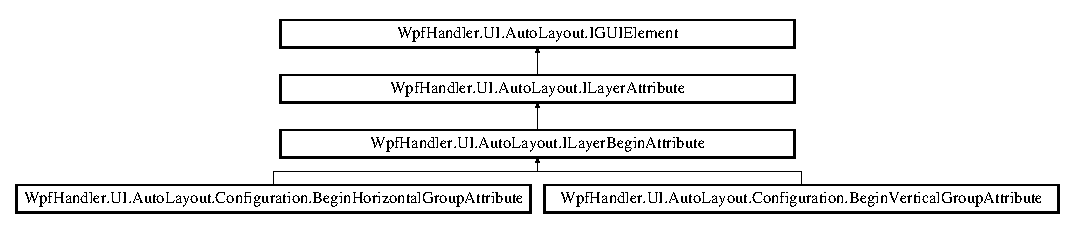
\includegraphics[height=2.635294cm]{d5/d7b/interface_wpf_handler_1_1_u_i_1_1_auto_layout_1_1_i_layer_begin_attribute}
\end{center}
\end{figure}
\subsection*{Additional Inherited Members}


\subsection{Detailed Description}
Attribute that cause new layer. 



The documentation for this interface was generated from the following file\+:\begin{DoxyCompactItemize}
\item 
D\+:/\+Work/\+Git\+Hub/wpf-\/handler/\+Wpf\+Handler/\+U\+I/\+Auto\+Layout/\+Interfaces/\+Layers/I\+Layer\+Begin\+Attribute.\+cs\end{DoxyCompactItemize}

\hypertarget{interface_wpf_handler_1_1_u_i_1_1_auto_layout_1_1_i_layer_end_attribute}{}\section{Wpf\+Handler.\+U\+I.\+Auto\+Layout.\+I\+Layer\+End\+Attribute Interface Reference}
\label{interface_wpf_handler_1_1_u_i_1_1_auto_layout_1_1_i_layer_end_attribute}\index{Wpf\+Handler.\+U\+I.\+Auto\+Layout.\+I\+Layer\+End\+Attribute@{Wpf\+Handler.\+U\+I.\+Auto\+Layout.\+I\+Layer\+End\+Attribute}}


Attribute that will cause end of work with current \mbox{\hyperlink{namespace_wpf_handler_1_1_u_i}{UI}} layer.  


Inheritance diagram for Wpf\+Handler.\+U\+I.\+Auto\+Layout.\+I\+Layer\+End\+Attribute\+:\begin{figure}[H]
\begin{center}
\leavevmode
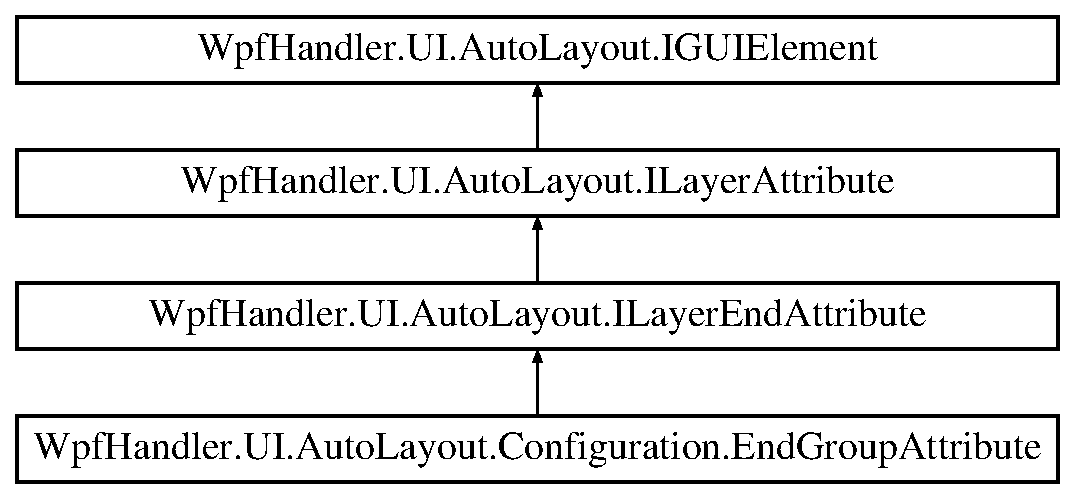
\includegraphics[height=4.000000cm]{df/d01/interface_wpf_handler_1_1_u_i_1_1_auto_layout_1_1_i_layer_end_attribute}
\end{center}
\end{figure}
\subsection*{Additional Inherited Members}


\subsection{Detailed Description}
Attribute that will cause end of work with current \mbox{\hyperlink{namespace_wpf_handler_1_1_u_i}{UI}} layer. 



The documentation for this interface was generated from the following file\+:\begin{DoxyCompactItemize}
\item 
D\+:/\+Work/\+Git\+Hub/wpf-\/handler/\+Wpf\+Handler/\+U\+I/\+Auto\+Layout/\+Interfaces/\+Layers/I\+Layer\+End\+Attribute.\+cs\end{DoxyCompactItemize}

\hypertarget{interface_wpf_handler_1_1_u_i_1_1_controls_1_1_i_layout_orientation}{}\section{Wpf\+Handler.\+U\+I.\+Controls.\+I\+Layout\+Orientation Interface Reference}
\label{interface_wpf_handler_1_1_u_i_1_1_controls_1_1_i_layout_orientation}\index{Wpf\+Handler.\+U\+I.\+Controls.\+I\+Layout\+Orientation@{Wpf\+Handler.\+U\+I.\+Controls.\+I\+Layout\+Orientation}}


Implementing of that interface make \mbox{\hyperlink{namespace_wpf_handler_1_1_u_i}{UI}} element compatible with orientation modifiers.  


Inheritance diagram for Wpf\+Handler.\+U\+I.\+Controls.\+I\+Layout\+Orientation\+:\begin{figure}[H]
\begin{center}
\leavevmode
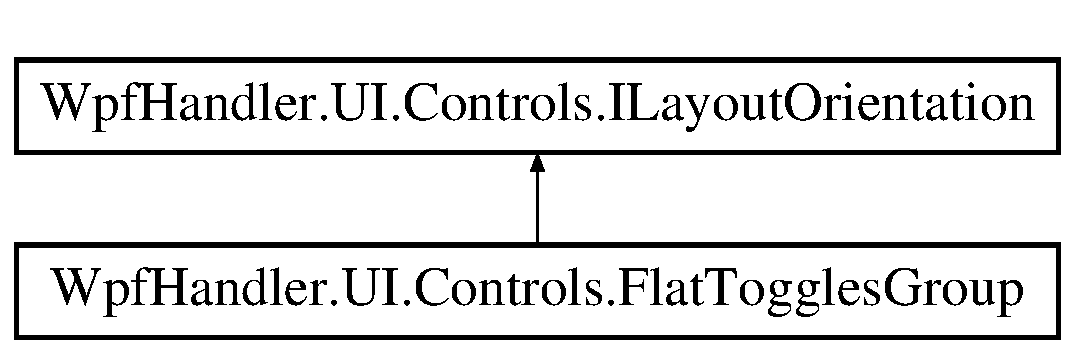
\includegraphics[height=2.000000cm]{d2/d03/interface_wpf_handler_1_1_u_i_1_1_controls_1_1_i_layout_orientation}
\end{center}
\end{figure}
\subsection*{Properties}
\begin{DoxyCompactItemize}
\item 
Orientation \mbox{\hyperlink{interface_wpf_handler_1_1_u_i_1_1_controls_1_1_i_layout_orientation_ae6ef94c906753022926767578498721a}{Orientation}}\hspace{0.3cm}{\ttfamily  \mbox{[}get, set\mbox{]}}
\begin{DoxyCompactList}\small\item\em Orientation of the \mbox{\hyperlink{namespace_wpf_handler_1_1_u_i}{UI}} element. \end{DoxyCompactList}\end{DoxyCompactItemize}


\subsection{Detailed Description}
Implementing of that interface make \mbox{\hyperlink{namespace_wpf_handler_1_1_u_i}{UI}} element compatible with orientation modifiers. 



\subsection{Property Documentation}
\mbox{\Hypertarget{interface_wpf_handler_1_1_u_i_1_1_controls_1_1_i_layout_orientation_ae6ef94c906753022926767578498721a}\label{interface_wpf_handler_1_1_u_i_1_1_controls_1_1_i_layout_orientation_ae6ef94c906753022926767578498721a}} 
\index{Wpf\+Handler\+::\+U\+I\+::\+Controls\+::\+I\+Layout\+Orientation@{Wpf\+Handler\+::\+U\+I\+::\+Controls\+::\+I\+Layout\+Orientation}!Orientation@{Orientation}}
\index{Orientation@{Orientation}!Wpf\+Handler\+::\+U\+I\+::\+Controls\+::\+I\+Layout\+Orientation@{Wpf\+Handler\+::\+U\+I\+::\+Controls\+::\+I\+Layout\+Orientation}}
\subsubsection{\texorpdfstring{Orientation}{Orientation}}
{\footnotesize\ttfamily Orientation Wpf\+Handler.\+U\+I.\+Controls.\+I\+Layout\+Orientation.\+Orientation\hspace{0.3cm}{\ttfamily [get]}, {\ttfamily [set]}}



Orientation of the \mbox{\hyperlink{namespace_wpf_handler_1_1_u_i}{UI}} element. 



The documentation for this interface was generated from the following file\+:\begin{DoxyCompactItemize}
\item 
D\+:/\+Work/\+Git\+Hub/wpf-\/handler/\+Wpf\+Handler/\+U\+I/\+Controls/I\+Layout\+Orientation.\+cs\end{DoxyCompactItemize}

\hypertarget{interface_wpf_handler_1_1_u_i_1_1_controls_1_1_i_layout_size}{}\section{Wpf\+Handler.\+U\+I.\+Controls.\+I\+Layout\+Size Interface Reference}
\label{interface_wpf_handler_1_1_u_i_1_1_controls_1_1_i_layout_size}\index{Wpf\+Handler.\+U\+I.\+Controls.\+I\+Layout\+Size@{Wpf\+Handler.\+U\+I.\+Controls.\+I\+Layout\+Size}}


Define properties for layout managment.  


Inheritance diagram for Wpf\+Handler.\+U\+I.\+Controls.\+I\+Layout\+Size\+:\begin{figure}[H]
\begin{center}
\leavevmode
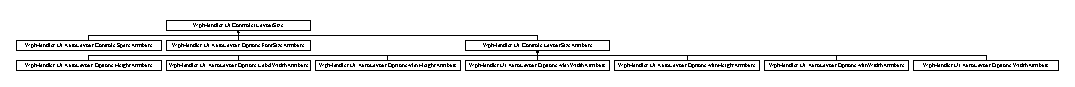
\includegraphics[height=0.727273cm]{d6/d39/interface_wpf_handler_1_1_u_i_1_1_controls_1_1_i_layout_size}
\end{center}
\end{figure}
\subsection*{Properties}
\begin{DoxyCompactItemize}
\item 
double \mbox{\hyperlink{interface_wpf_handler_1_1_u_i_1_1_controls_1_1_i_layout_size_ab6305d7396e1e85d864d110db689331f}{Size}}\hspace{0.3cm}{\ttfamily  \mbox{[}get, set\mbox{]}}
\begin{DoxyCompactList}\small\item\em Value applied to layout property. \end{DoxyCompactList}\end{DoxyCompactItemize}


\subsection{Detailed Description}
Define properties for layout managment. 



\subsection{Property Documentation}
\mbox{\Hypertarget{interface_wpf_handler_1_1_u_i_1_1_controls_1_1_i_layout_size_ab6305d7396e1e85d864d110db689331f}\label{interface_wpf_handler_1_1_u_i_1_1_controls_1_1_i_layout_size_ab6305d7396e1e85d864d110db689331f}} 
\index{Wpf\+Handler\+::\+U\+I\+::\+Controls\+::\+I\+Layout\+Size@{Wpf\+Handler\+::\+U\+I\+::\+Controls\+::\+I\+Layout\+Size}!Size@{Size}}
\index{Size@{Size}!Wpf\+Handler\+::\+U\+I\+::\+Controls\+::\+I\+Layout\+Size@{Wpf\+Handler\+::\+U\+I\+::\+Controls\+::\+I\+Layout\+Size}}
\subsubsection{\texorpdfstring{Size}{Size}}
{\footnotesize\ttfamily double Wpf\+Handler.\+U\+I.\+Controls.\+I\+Layout\+Size.\+Size\hspace{0.3cm}{\ttfamily [get]}, {\ttfamily [set]}}



Value applied to layout property. 



The documentation for this interface was generated from the following file\+:\begin{DoxyCompactItemize}
\item 
D\+:/\+Work/\+Git\+Hub/wpf-\/handler/\+Wpf\+Handler/\+U\+I/\+Controls/I\+Layout\+Size.\+cs\end{DoxyCompactItemize}

\hypertarget{class_wpf_handler_1_1_u_i_1_1_auto_layout_1_1_markups_1_1_i_list_compatible_attribute}{}\section{Wpf\+Handler.\+U\+I.\+Auto\+Layout.\+Markups.\+I\+List\+Compatible\+Attribute Class Reference}
\label{class_wpf_handler_1_1_u_i_1_1_auto_layout_1_1_markups_1_1_i_list_compatible_attribute}\index{Wpf\+Handler.\+U\+I.\+Auto\+Layout.\+Markups.\+I\+List\+Compatible\+Attribute@{Wpf\+Handler.\+U\+I.\+Auto\+Layout.\+Markups.\+I\+List\+Compatible\+Attribute}}


Marks a G\+UI element as compatible with I\+List members.  


Inheritance diagram for Wpf\+Handler.\+U\+I.\+Auto\+Layout.\+Markups.\+I\+List\+Compatible\+Attribute\+:\begin{figure}[H]
\begin{center}
\leavevmode
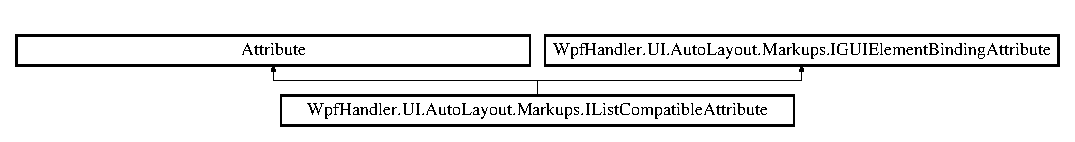
\includegraphics[height=1.462141cm]{d3/df0/class_wpf_handler_1_1_u_i_1_1_auto_layout_1_1_markups_1_1_i_list_compatible_attribute}
\end{center}
\end{figure}


\subsection{Detailed Description}
Marks a G\+UI element as compatible with I\+List members. 

Class with that attribute will be allowed only for displaying I\+List members. Any other specifing will not has any effect. 

The documentation for this class was generated from the following file\+:\begin{DoxyCompactItemize}
\item 
D\+:/\+Work/\+Git\+Hub/wpf-\/handler/\+Wpf\+Handler/\+U\+I/\+Auto\+Layout/\+Markups/I\+List\+Compatible\+Attribute.\+cs\end{DoxyCompactItemize}

\hypertarget{interface_wpf_handler_1_1_plugins_1_1_i_plugin}{}\section{Wpf\+Handler.\+Plugins.\+I\+Plugin Interface Reference}
\label{interface_wpf_handler_1_1_plugins_1_1_i_plugin}\index{Wpf\+Handler.\+Plugins.\+I\+Plugin@{Wpf\+Handler.\+Plugins.\+I\+Plugin}}


Interface that allow to create a plugin that can be connect to client application.  


\subsection*{Public Member Functions}
\begin{DoxyCompactItemize}
\item 
void \mbox{\hyperlink{interface_wpf_handler_1_1_plugins_1_1_i_plugin_aabe1a8e5680ebeb37f96ffe86b6123e9}{On\+Start}} (object sender)
\begin{DoxyCompactList}\small\item\em Method that will has been calling when menu item would press. Use to apply executable part of the plugin. \end{DoxyCompactList}\end{DoxyCompactItemize}
\subsection*{Properties}
\begin{DoxyCompactItemize}
\item 
\mbox{\hyperlink{class_wpf_handler_1_1_plugins_1_1_menu_item_meta}{Menu\+Item\+Meta}} \mbox{\hyperlink{interface_wpf_handler_1_1_plugins_1_1_i_plugin_a654e20458e4e44b69c9de0be25a8d9af}{Meta}}\hspace{0.3cm}{\ttfamily  \mbox{[}get, set\mbox{]}}
\begin{DoxyCompactList}\small\item\em Meta data that contains description for main menu integration. \end{DoxyCompactList}\end{DoxyCompactItemize}


\subsection{Detailed Description}
Interface that allow to create a plugin that can be connect to client application. 



\subsection{Member Function Documentation}
\mbox{\Hypertarget{interface_wpf_handler_1_1_plugins_1_1_i_plugin_aabe1a8e5680ebeb37f96ffe86b6123e9}\label{interface_wpf_handler_1_1_plugins_1_1_i_plugin_aabe1a8e5680ebeb37f96ffe86b6123e9}} 
\index{Wpf\+Handler\+::\+Plugins\+::\+I\+Plugin@{Wpf\+Handler\+::\+Plugins\+::\+I\+Plugin}!On\+Start@{On\+Start}}
\index{On\+Start@{On\+Start}!Wpf\+Handler\+::\+Plugins\+::\+I\+Plugin@{Wpf\+Handler\+::\+Plugins\+::\+I\+Plugin}}
\subsubsection{\texorpdfstring{On\+Start()}{OnStart()}}
{\footnotesize\ttfamily void Wpf\+Handler.\+Plugins.\+I\+Plugin.\+On\+Start (\begin{DoxyParamCaption}\item[{object}]{sender }\end{DoxyParamCaption})}



Method that will has been calling when menu item would press. Use to apply executable part of the plugin. 



\subsection{Property Documentation}
\mbox{\Hypertarget{interface_wpf_handler_1_1_plugins_1_1_i_plugin_a654e20458e4e44b69c9de0be25a8d9af}\label{interface_wpf_handler_1_1_plugins_1_1_i_plugin_a654e20458e4e44b69c9de0be25a8d9af}} 
\index{Wpf\+Handler\+::\+Plugins\+::\+I\+Plugin@{Wpf\+Handler\+::\+Plugins\+::\+I\+Plugin}!Meta@{Meta}}
\index{Meta@{Meta}!Wpf\+Handler\+::\+Plugins\+::\+I\+Plugin@{Wpf\+Handler\+::\+Plugins\+::\+I\+Plugin}}
\subsubsection{\texorpdfstring{Meta}{Meta}}
{\footnotesize\ttfamily \mbox{\hyperlink{class_wpf_handler_1_1_plugins_1_1_menu_item_meta}{Menu\+Item\+Meta}} Wpf\+Handler.\+Plugins.\+I\+Plugin.\+Meta\hspace{0.3cm}{\ttfamily [get]}, {\ttfamily [set]}}



Meta data that contains description for main menu integration. 



The documentation for this interface was generated from the following file\+:\begin{DoxyCompactItemize}
\item 
D\+:/\+Work/\+Git\+Hub/wpf-\/handler/\+Wpf\+Handler/\+Plugins/\+Interfaces/I\+Plugin.\+cs\end{DoxyCompactItemize}

\hypertarget{interface_wpf_handler_1_1_plugins_1_1_i_plugin_settings}{}\section{Wpf\+Handler.\+Plugins.\+I\+Plugin\+Settings Interface Reference}
\label{interface_wpf_handler_1_1_plugins_1_1_i_plugin_settings}\index{Wpf\+Handler.\+Plugins.\+I\+Plugin\+Settings@{Wpf\+Handler.\+Plugins.\+I\+Plugin\+Settings}}


Provide possibility to implement setting ui block in application.  


\subsection*{Properties}
\begin{DoxyCompactItemize}
\item 
\mbox{\hyperlink{class_wpf_handler_1_1_plugins_1_1_menu_item_meta}{Menu\+Item\+Meta}} \mbox{\hyperlink{interface_wpf_handler_1_1_plugins_1_1_i_plugin_settings_a63a2624a2e5f76e870817ebb292ec462}{Meta}}\hspace{0.3cm}{\ttfamily  \mbox{[}get, set\mbox{]}}
\begin{DoxyCompactList}\small\item\em Meta data that contains description for main menu integration. \end{DoxyCompactList}\item 
User\+Control \mbox{\hyperlink{interface_wpf_handler_1_1_plugins_1_1_i_plugin_settings_a61126c998a55b28a6f7f79905621fc54}{G\+UI}}\hspace{0.3cm}{\ttfamily  \mbox{[}get\mbox{]}}
\begin{DoxyCompactList}\small\item\em Return control that can be displayed as block of settings menu. \end{DoxyCompactList}\end{DoxyCompactItemize}


\subsection{Detailed Description}
Provide possibility to implement setting ui block in application. 



\subsection{Property Documentation}
\mbox{\Hypertarget{interface_wpf_handler_1_1_plugins_1_1_i_plugin_settings_a61126c998a55b28a6f7f79905621fc54}\label{interface_wpf_handler_1_1_plugins_1_1_i_plugin_settings_a61126c998a55b28a6f7f79905621fc54}} 
\index{Wpf\+Handler\+::\+Plugins\+::\+I\+Plugin\+Settings@{Wpf\+Handler\+::\+Plugins\+::\+I\+Plugin\+Settings}!G\+UI@{G\+UI}}
\index{G\+UI@{G\+UI}!Wpf\+Handler\+::\+Plugins\+::\+I\+Plugin\+Settings@{Wpf\+Handler\+::\+Plugins\+::\+I\+Plugin\+Settings}}
\subsubsection{\texorpdfstring{G\+UI}{GUI}}
{\footnotesize\ttfamily User\+Control Wpf\+Handler.\+Plugins.\+I\+Plugin\+Settings.\+G\+UI\hspace{0.3cm}{\ttfamily [get]}}



Return control that can be displayed as block of settings menu. 

\mbox{\Hypertarget{interface_wpf_handler_1_1_plugins_1_1_i_plugin_settings_a63a2624a2e5f76e870817ebb292ec462}\label{interface_wpf_handler_1_1_plugins_1_1_i_plugin_settings_a63a2624a2e5f76e870817ebb292ec462}} 
\index{Wpf\+Handler\+::\+Plugins\+::\+I\+Plugin\+Settings@{Wpf\+Handler\+::\+Plugins\+::\+I\+Plugin\+Settings}!Meta@{Meta}}
\index{Meta@{Meta}!Wpf\+Handler\+::\+Plugins\+::\+I\+Plugin\+Settings@{Wpf\+Handler\+::\+Plugins\+::\+I\+Plugin\+Settings}}
\subsubsection{\texorpdfstring{Meta}{Meta}}
{\footnotesize\ttfamily \mbox{\hyperlink{class_wpf_handler_1_1_plugins_1_1_menu_item_meta}{Menu\+Item\+Meta}} Wpf\+Handler.\+Plugins.\+I\+Plugin\+Settings.\+Meta\hspace{0.3cm}{\ttfamily [get]}, {\ttfamily [set]}}



Meta data that contains description for main menu integration. 



The documentation for this interface was generated from the following file\+:\begin{DoxyCompactItemize}
\item 
D\+:/\+Work/\+Git\+Hub/wpf-\/handler/\+Wpf\+Handler/\+Plugins/\+Interfaces/I\+Plugin\+Settings.\+cs\end{DoxyCompactItemize}

\hypertarget{interface_wpf_handler_1_1_u_i_1_1_controls_1_1_i_toggle_control}{}\section{Wpf\+Handler.\+U\+I.\+Controls.\+I\+Toggle\+Control Interface Reference}
\label{interface_wpf_handler_1_1_u_i_1_1_controls_1_1_i_toggle_control}\index{Wpf\+Handler.\+U\+I.\+Controls.\+I\+Toggle\+Control@{Wpf\+Handler.\+U\+I.\+Controls.\+I\+Toggle\+Control}}


Provides standardized way to operate toggle state of the element.  


Inheritance diagram for Wpf\+Handler.\+U\+I.\+Controls.\+I\+Toggle\+Control\+:\begin{figure}[H]
\begin{center}
\leavevmode
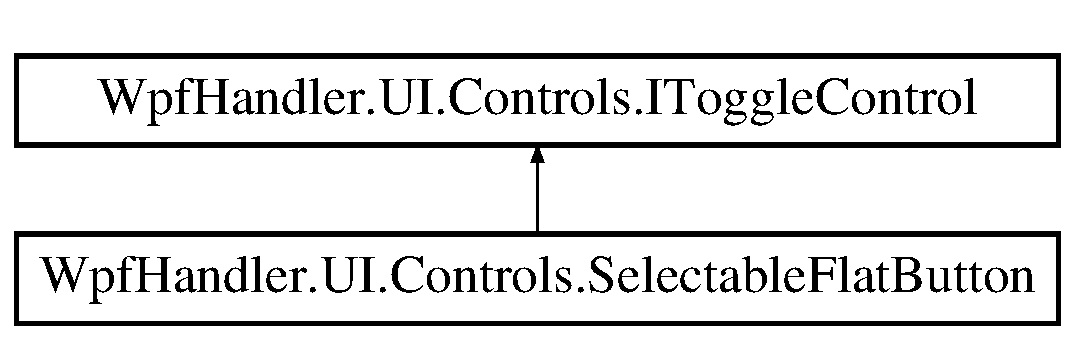
\includegraphics[height=2.000000cm]{d5/db4/interface_wpf_handler_1_1_u_i_1_1_controls_1_1_i_toggle_control}
\end{center}
\end{figure}
\subsection*{Properties}
\begin{DoxyCompactItemize}
\item 
bool \mbox{\hyperlink{interface_wpf_handler_1_1_u_i_1_1_controls_1_1_i_toggle_control_a7262e3301c8625f3104105ed336bc427}{Selected}}\hspace{0.3cm}{\ttfamily  \mbox{[}get, set\mbox{]}}
\begin{DoxyCompactList}\small\item\em Is that element selected. \end{DoxyCompactList}\item 
string \mbox{\hyperlink{interface_wpf_handler_1_1_u_i_1_1_controls_1_1_i_toggle_control_a3ad83163a8f21262b4d48d831ad72541}{Group}}\hspace{0.3cm}{\ttfamily  \mbox{[}get, set\mbox{]}}
\begin{DoxyCompactList}\small\item\em Group of buttons that will allow auto deselect other buttons from that group. \end{DoxyCompactList}\item 
bool \mbox{\hyperlink{interface_wpf_handler_1_1_u_i_1_1_controls_1_1_i_toggle_control_a459178217d5156bb32ac1fd9eef9fd20}{Multi\+Selection}}\hspace{0.3cm}{\ttfamily  \mbox{[}get, set\mbox{]}}
\begin{DoxyCompactList}\small\item\em Is group allow few selected buttons in one group. \end{DoxyCompactList}\end{DoxyCompactItemize}


\subsection{Detailed Description}
Provides standardized way to operate toggle state of the element. 



\subsection{Property Documentation}
\mbox{\Hypertarget{interface_wpf_handler_1_1_u_i_1_1_controls_1_1_i_toggle_control_a3ad83163a8f21262b4d48d831ad72541}\label{interface_wpf_handler_1_1_u_i_1_1_controls_1_1_i_toggle_control_a3ad83163a8f21262b4d48d831ad72541}} 
\index{Wpf\+Handler\+::\+U\+I\+::\+Controls\+::\+I\+Toggle\+Control@{Wpf\+Handler\+::\+U\+I\+::\+Controls\+::\+I\+Toggle\+Control}!Group@{Group}}
\index{Group@{Group}!Wpf\+Handler\+::\+U\+I\+::\+Controls\+::\+I\+Toggle\+Control@{Wpf\+Handler\+::\+U\+I\+::\+Controls\+::\+I\+Toggle\+Control}}
\subsubsection{\texorpdfstring{Group}{Group}}
{\footnotesize\ttfamily string Wpf\+Handler.\+U\+I.\+Controls.\+I\+Toggle\+Control.\+Group\hspace{0.3cm}{\ttfamily [get]}, {\ttfamily [set]}}



Group of buttons that will allow auto deselect other buttons from that group. 

\mbox{\Hypertarget{interface_wpf_handler_1_1_u_i_1_1_controls_1_1_i_toggle_control_a459178217d5156bb32ac1fd9eef9fd20}\label{interface_wpf_handler_1_1_u_i_1_1_controls_1_1_i_toggle_control_a459178217d5156bb32ac1fd9eef9fd20}} 
\index{Wpf\+Handler\+::\+U\+I\+::\+Controls\+::\+I\+Toggle\+Control@{Wpf\+Handler\+::\+U\+I\+::\+Controls\+::\+I\+Toggle\+Control}!Multi\+Selection@{Multi\+Selection}}
\index{Multi\+Selection@{Multi\+Selection}!Wpf\+Handler\+::\+U\+I\+::\+Controls\+::\+I\+Toggle\+Control@{Wpf\+Handler\+::\+U\+I\+::\+Controls\+::\+I\+Toggle\+Control}}
\subsubsection{\texorpdfstring{Multi\+Selection}{MultiSelection}}
{\footnotesize\ttfamily bool Wpf\+Handler.\+U\+I.\+Controls.\+I\+Toggle\+Control.\+Multi\+Selection\hspace{0.3cm}{\ttfamily [get]}, {\ttfamily [set]}}



Is group allow few selected buttons in one group. 

\mbox{\Hypertarget{interface_wpf_handler_1_1_u_i_1_1_controls_1_1_i_toggle_control_a7262e3301c8625f3104105ed336bc427}\label{interface_wpf_handler_1_1_u_i_1_1_controls_1_1_i_toggle_control_a7262e3301c8625f3104105ed336bc427}} 
\index{Wpf\+Handler\+::\+U\+I\+::\+Controls\+::\+I\+Toggle\+Control@{Wpf\+Handler\+::\+U\+I\+::\+Controls\+::\+I\+Toggle\+Control}!Selected@{Selected}}
\index{Selected@{Selected}!Wpf\+Handler\+::\+U\+I\+::\+Controls\+::\+I\+Toggle\+Control@{Wpf\+Handler\+::\+U\+I\+::\+Controls\+::\+I\+Toggle\+Control}}
\subsubsection{\texorpdfstring{Selected}{Selected}}
{\footnotesize\ttfamily bool Wpf\+Handler.\+U\+I.\+Controls.\+I\+Toggle\+Control.\+Selected\hspace{0.3cm}{\ttfamily [get]}, {\ttfamily [set]}}



Is that element selected. 



The documentation for this interface was generated from the following file\+:\begin{DoxyCompactItemize}
\item 
D\+:/\+Work/\+Git\+Hub/wpf-\/handler/\+Wpf\+Handler/\+U\+I/\+Controls/I\+Toggle\+Control.\+cs\end{DoxyCompactItemize}

\hypertarget{class_wpf_handler_1_1_u_i_1_1_auto_layout_1_1_controls_1_1_label_attribute}{}\section{Wpf\+Handler.\+U\+I.\+Auto\+Layout.\+Controls.\+Label\+Attribute Class Reference}
\label{class_wpf_handler_1_1_u_i_1_1_auto_layout_1_1_controls_1_1_label_attribute}\index{Wpf\+Handler.\+U\+I.\+Auto\+Layout.\+Controls.\+Label\+Attribute@{Wpf\+Handler.\+U\+I.\+Auto\+Layout.\+Controls.\+Label\+Attribute}}


Allow to add custom label element to the \mbox{\hyperlink{namespace_wpf_handler_1_1_u_i}{UI}}.  


Inheritance diagram for Wpf\+Handler.\+U\+I.\+Auto\+Layout.\+Controls.\+Label\+Attribute\+:\begin{figure}[H]
\begin{center}
\leavevmode
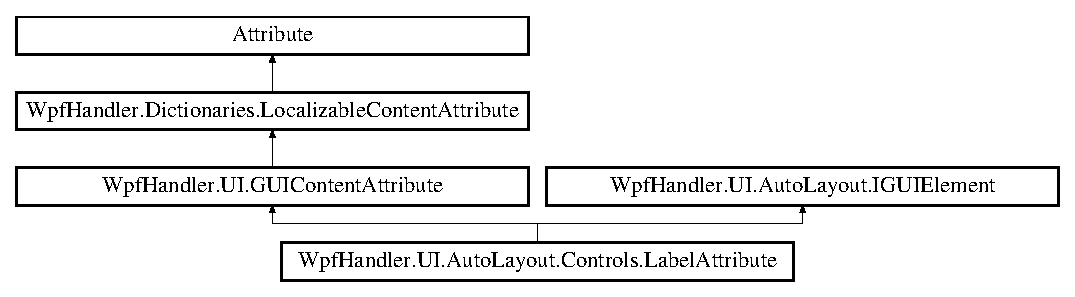
\includegraphics[height=4.000000cm]{d9/d7c/class_wpf_handler_1_1_u_i_1_1_auto_layout_1_1_controls_1_1_label_attribute}
\end{center}
\end{figure}
\subsection*{Public Member Functions}
\begin{DoxyCompactItemize}
\item 
\mbox{\hyperlink{class_wpf_handler_1_1_u_i_1_1_auto_layout_1_1_controls_1_1_label_attribute_af52c1a4d96d9ab17f369a6c6423f58fb}{Label\+Attribute}} (string title)
\begin{DoxyCompactList}\small\item\em Auto initialize content with shared title value. \end{DoxyCompactList}\item 
\mbox{\hyperlink{class_wpf_handler_1_1_u_i_1_1_auto_layout_1_1_controls_1_1_label_attribute_a961e0cd1faee5baad4ced251193adcc4}{Label\+Attribute}} (string title, string description)
\begin{DoxyCompactList}\small\item\em Constructor that allow to set title. \end{DoxyCompactList}\item 
\mbox{\hyperlink{class_wpf_handler_1_1_u_i_1_1_auto_layout_1_1_controls_1_1_label_attribute_ae3fc540124479e4cdc343ab23ae1a1c9}{Label\+Attribute}} (string default\+Title, string default\+Description, string decription\+Localization\+Resourse\+Key)
\begin{DoxyCompactList}\small\item\em Initialize all allowed fields. \end{DoxyCompactList}\item 
\mbox{\hyperlink{class_wpf_handler_1_1_u_i_1_1_auto_layout_1_1_controls_1_1_label_attribute_abfc5ebdb910630168db5f10fdbb713b7}{Label\+Attribute}} (string default\+Title, string default\+Description, string title\+Localization\+Resourse\+Key, string decription\+Localization\+Resourse\+Key)
\begin{DoxyCompactList}\small\item\em Initialize all allowed fields. \end{DoxyCompactList}\item 
virtual void \mbox{\hyperlink{class_wpf_handler_1_1_u_i_1_1_auto_layout_1_1_controls_1_1_label_attribute_a86bdaaa6d028cbdee8536138e63d0159}{On\+G\+UI}} (ref \mbox{\hyperlink{class_wpf_handler_1_1_u_i_1_1_auto_layout_1_1_layout_layer}{Layout\+Layer}} layer, params object\mbox{[}$\,$\mbox{]} args)
\begin{DoxyCompactList}\small\item\em Spawn label element into the \mbox{\hyperlink{namespace_wpf_handler_1_1_u_i}{UI}}. \end{DoxyCompactList}\item 
override void \mbox{\hyperlink{class_wpf_handler_1_1_u_i_1_1_auto_layout_1_1_controls_1_1_label_attribute_a3ed5f61dc946ffd5ce385cc4ef60362d}{Languages\+Dictionaries\+Updated}} ()
\begin{DoxyCompactList}\small\item\em T\+O\+DO\+: Callback that occurs when content dictionaries are reloaded. Updating label\textquotesingle{}s content. \end{DoxyCompactList}\end{DoxyCompactItemize}
\subsection*{Additional Inherited Members}


\subsection{Detailed Description}
Allow to add custom label element to the \mbox{\hyperlink{namespace_wpf_handler_1_1_u_i}{UI}}. 



\subsection{Constructor \& Destructor Documentation}
\mbox{\Hypertarget{class_wpf_handler_1_1_u_i_1_1_auto_layout_1_1_controls_1_1_label_attribute_af52c1a4d96d9ab17f369a6c6423f58fb}\label{class_wpf_handler_1_1_u_i_1_1_auto_layout_1_1_controls_1_1_label_attribute_af52c1a4d96d9ab17f369a6c6423f58fb}} 
\index{Wpf\+Handler\+::\+U\+I\+::\+Auto\+Layout\+::\+Controls\+::\+Label\+Attribute@{Wpf\+Handler\+::\+U\+I\+::\+Auto\+Layout\+::\+Controls\+::\+Label\+Attribute}!Label\+Attribute@{Label\+Attribute}}
\index{Label\+Attribute@{Label\+Attribute}!Wpf\+Handler\+::\+U\+I\+::\+Auto\+Layout\+::\+Controls\+::\+Label\+Attribute@{Wpf\+Handler\+::\+U\+I\+::\+Auto\+Layout\+::\+Controls\+::\+Label\+Attribute}}
\subsubsection{\texorpdfstring{Label\+Attribute()}{LabelAttribute()}\hspace{0.1cm}{\footnotesize\ttfamily [1/4]}}
{\footnotesize\ttfamily Wpf\+Handler.\+U\+I.\+Auto\+Layout.\+Controls.\+Label\+Attribute.\+Label\+Attribute (\begin{DoxyParamCaption}\item[{string}]{title }\end{DoxyParamCaption})}



Auto initialize content with shared title value. 


\begin{DoxyParams}{Parameters}
{\em title} & Title that will be showed up into the label.\\
\hline
\end{DoxyParams}
\mbox{\Hypertarget{class_wpf_handler_1_1_u_i_1_1_auto_layout_1_1_controls_1_1_label_attribute_a961e0cd1faee5baad4ced251193adcc4}\label{class_wpf_handler_1_1_u_i_1_1_auto_layout_1_1_controls_1_1_label_attribute_a961e0cd1faee5baad4ced251193adcc4}} 
\index{Wpf\+Handler\+::\+U\+I\+::\+Auto\+Layout\+::\+Controls\+::\+Label\+Attribute@{Wpf\+Handler\+::\+U\+I\+::\+Auto\+Layout\+::\+Controls\+::\+Label\+Attribute}!Label\+Attribute@{Label\+Attribute}}
\index{Label\+Attribute@{Label\+Attribute}!Wpf\+Handler\+::\+U\+I\+::\+Auto\+Layout\+::\+Controls\+::\+Label\+Attribute@{Wpf\+Handler\+::\+U\+I\+::\+Auto\+Layout\+::\+Controls\+::\+Label\+Attribute}}
\subsubsection{\texorpdfstring{Label\+Attribute()}{LabelAttribute()}\hspace{0.1cm}{\footnotesize\ttfamily [2/4]}}
{\footnotesize\ttfamily Wpf\+Handler.\+U\+I.\+Auto\+Layout.\+Controls.\+Label\+Attribute.\+Label\+Attribute (\begin{DoxyParamCaption}\item[{string}]{title,  }\item[{string}]{description }\end{DoxyParamCaption})}



Constructor that allow to set title. 


\begin{DoxyParams}{Parameters}
{\em title} & Title of that element.\\
\hline
{\em description} & Description of that element.\\
\hline
\end{DoxyParams}
\mbox{\Hypertarget{class_wpf_handler_1_1_u_i_1_1_auto_layout_1_1_controls_1_1_label_attribute_ae3fc540124479e4cdc343ab23ae1a1c9}\label{class_wpf_handler_1_1_u_i_1_1_auto_layout_1_1_controls_1_1_label_attribute_ae3fc540124479e4cdc343ab23ae1a1c9}} 
\index{Wpf\+Handler\+::\+U\+I\+::\+Auto\+Layout\+::\+Controls\+::\+Label\+Attribute@{Wpf\+Handler\+::\+U\+I\+::\+Auto\+Layout\+::\+Controls\+::\+Label\+Attribute}!Label\+Attribute@{Label\+Attribute}}
\index{Label\+Attribute@{Label\+Attribute}!Wpf\+Handler\+::\+U\+I\+::\+Auto\+Layout\+::\+Controls\+::\+Label\+Attribute@{Wpf\+Handler\+::\+U\+I\+::\+Auto\+Layout\+::\+Controls\+::\+Label\+Attribute}}
\subsubsection{\texorpdfstring{Label\+Attribute()}{LabelAttribute()}\hspace{0.1cm}{\footnotesize\ttfamily [3/4]}}
{\footnotesize\ttfamily Wpf\+Handler.\+U\+I.\+Auto\+Layout.\+Controls.\+Label\+Attribute.\+Label\+Attribute (\begin{DoxyParamCaption}\item[{string}]{default\+Title,  }\item[{string}]{default\+Description,  }\item[{string}]{decription\+Localization\+Resourse\+Key }\end{DoxyParamCaption})}



Initialize all allowed fields. 


\begin{DoxyParams}{Parameters}
{\em default\+Title} & Title that would be used by default if localization dictionary not found.\\
\hline
{\em default\+Description} & Default description if localization dictionary not found.\\
\hline
{\em decription\+Localization\+Resourse\+Key} & Key of description content in localized dynamic dictionary.\\
\hline
\end{DoxyParams}
\mbox{\Hypertarget{class_wpf_handler_1_1_u_i_1_1_auto_layout_1_1_controls_1_1_label_attribute_abfc5ebdb910630168db5f10fdbb713b7}\label{class_wpf_handler_1_1_u_i_1_1_auto_layout_1_1_controls_1_1_label_attribute_abfc5ebdb910630168db5f10fdbb713b7}} 
\index{Wpf\+Handler\+::\+U\+I\+::\+Auto\+Layout\+::\+Controls\+::\+Label\+Attribute@{Wpf\+Handler\+::\+U\+I\+::\+Auto\+Layout\+::\+Controls\+::\+Label\+Attribute}!Label\+Attribute@{Label\+Attribute}}
\index{Label\+Attribute@{Label\+Attribute}!Wpf\+Handler\+::\+U\+I\+::\+Auto\+Layout\+::\+Controls\+::\+Label\+Attribute@{Wpf\+Handler\+::\+U\+I\+::\+Auto\+Layout\+::\+Controls\+::\+Label\+Attribute}}
\subsubsection{\texorpdfstring{Label\+Attribute()}{LabelAttribute()}\hspace{0.1cm}{\footnotesize\ttfamily [4/4]}}
{\footnotesize\ttfamily Wpf\+Handler.\+U\+I.\+Auto\+Layout.\+Controls.\+Label\+Attribute.\+Label\+Attribute (\begin{DoxyParamCaption}\item[{string}]{default\+Title,  }\item[{string}]{default\+Description,  }\item[{string}]{title\+Localization\+Resourse\+Key,  }\item[{string}]{decription\+Localization\+Resourse\+Key }\end{DoxyParamCaption})}



Initialize all allowed fields. 


\begin{DoxyParams}{Parameters}
{\em default\+Title} & Title that would be used by default if localization dictionary not found.\\
\hline
{\em default\+Description} & Default description if localization dictionary not found.\\
\hline
{\em title\+Localization\+Resourse\+Key} & Key of title content in localized dynamic dictionary.\\
\hline
{\em decription\+Localization\+Resourse\+Key} & Key of description content in localized dynamic dictionary.\\
\hline
\end{DoxyParams}


\subsection{Member Function Documentation}
\mbox{\Hypertarget{class_wpf_handler_1_1_u_i_1_1_auto_layout_1_1_controls_1_1_label_attribute_a3ed5f61dc946ffd5ce385cc4ef60362d}\label{class_wpf_handler_1_1_u_i_1_1_auto_layout_1_1_controls_1_1_label_attribute_a3ed5f61dc946ffd5ce385cc4ef60362d}} 
\index{Wpf\+Handler\+::\+U\+I\+::\+Auto\+Layout\+::\+Controls\+::\+Label\+Attribute@{Wpf\+Handler\+::\+U\+I\+::\+Auto\+Layout\+::\+Controls\+::\+Label\+Attribute}!Languages\+Dictionaries\+Updated@{Languages\+Dictionaries\+Updated}}
\index{Languages\+Dictionaries\+Updated@{Languages\+Dictionaries\+Updated}!Wpf\+Handler\+::\+U\+I\+::\+Auto\+Layout\+::\+Controls\+::\+Label\+Attribute@{Wpf\+Handler\+::\+U\+I\+::\+Auto\+Layout\+::\+Controls\+::\+Label\+Attribute}}
\subsubsection{\texorpdfstring{Languages\+Dictionaries\+Updated()}{LanguagesDictionariesUpdated()}}
{\footnotesize\ttfamily override void Wpf\+Handler.\+U\+I.\+Auto\+Layout.\+Controls.\+Label\+Attribute.\+Languages\+Dictionaries\+Updated (\begin{DoxyParamCaption}{ }\end{DoxyParamCaption})\hspace{0.3cm}{\ttfamily [virtual]}}



T\+O\+DO\+: Callback that occurs when content dictionaries are reloaded. Updating label\textquotesingle{}s content. 



Implements \mbox{\hyperlink{class_wpf_handler_1_1_dictionaries_1_1_localizable_content_attribute_a001e110c7ad42422bc02a44d9eedc801}{Wpf\+Handler.\+Dictionaries.\+Localizable\+Content\+Attribute}}.

\mbox{\Hypertarget{class_wpf_handler_1_1_u_i_1_1_auto_layout_1_1_controls_1_1_label_attribute_a86bdaaa6d028cbdee8536138e63d0159}\label{class_wpf_handler_1_1_u_i_1_1_auto_layout_1_1_controls_1_1_label_attribute_a86bdaaa6d028cbdee8536138e63d0159}} 
\index{Wpf\+Handler\+::\+U\+I\+::\+Auto\+Layout\+::\+Controls\+::\+Label\+Attribute@{Wpf\+Handler\+::\+U\+I\+::\+Auto\+Layout\+::\+Controls\+::\+Label\+Attribute}!On\+G\+UI@{On\+G\+UI}}
\index{On\+G\+UI@{On\+G\+UI}!Wpf\+Handler\+::\+U\+I\+::\+Auto\+Layout\+::\+Controls\+::\+Label\+Attribute@{Wpf\+Handler\+::\+U\+I\+::\+Auto\+Layout\+::\+Controls\+::\+Label\+Attribute}}
\subsubsection{\texorpdfstring{On\+G\+U\+I()}{OnGUI()}}
{\footnotesize\ttfamily virtual void Wpf\+Handler.\+U\+I.\+Auto\+Layout.\+Controls.\+Label\+Attribute.\+On\+G\+UI (\begin{DoxyParamCaption}\item[{ref \mbox{\hyperlink{class_wpf_handler_1_1_u_i_1_1_auto_layout_1_1_layout_layer}{Layout\+Layer}}}]{layer,  }\item[{params object \mbox{[}$\,$\mbox{]}}]{args }\end{DoxyParamCaption})\hspace{0.3cm}{\ttfamily [virtual]}}



Spawn label element into the \mbox{\hyperlink{namespace_wpf_handler_1_1_u_i}{UI}}. 


\begin{DoxyParams}{Parameters}
{\em layer} & \\
\hline
{\em args} & \\
\hline
\end{DoxyParams}


The documentation for this class was generated from the following file\+:\begin{DoxyCompactItemize}
\item 
D\+:/\+Work/\+Git\+Hub/wpf-\/handler/\+Wpf\+Handler/\+U\+I/\+Auto\+Layout/\+Controls/Label\+Attribute.\+cs\end{DoxyCompactItemize}

\hypertarget{class_wpf_handler_1_1_u_i_1_1_auto_layout_1_1_options_1_1_label_width_attribute}{}\section{Wpf\+Handler.\+U\+I.\+Auto\+Layout.\+Options.\+Label\+Width\+Attribute Class Reference}
\label{class_wpf_handler_1_1_u_i_1_1_auto_layout_1_1_options_1_1_label_width_attribute}\index{Wpf\+Handler.\+U\+I.\+Auto\+Layout.\+Options.\+Label\+Width\+Attribute@{Wpf\+Handler.\+U\+I.\+Auto\+Layout.\+Options.\+Label\+Width\+Attribute}}


Redefines lable width for the I\+Lable objects.  


Inheritance diagram for Wpf\+Handler.\+U\+I.\+Auto\+Layout.\+Options.\+Label\+Width\+Attribute\+:\begin{figure}[H]
\begin{center}
\leavevmode
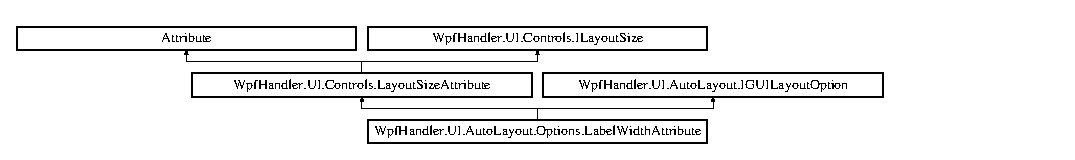
\includegraphics[height=1.696970cm]{d2/d77/class_wpf_handler_1_1_u_i_1_1_auto_layout_1_1_options_1_1_label_width_attribute}
\end{center}
\end{figure}
\subsection*{Public Member Functions}
\begin{DoxyCompactItemize}
\item 
\mbox{\hyperlink{class_wpf_handler_1_1_u_i_1_1_auto_layout_1_1_options_1_1_label_width_attribute_a466768b6dfd74a49bcae860cb52ab7ab}{Label\+Width\+Attribute}} ()
\begin{DoxyCompactList}\small\item\em Default constructor. Using auto width. \end{DoxyCompactList}\item 
\mbox{\hyperlink{class_wpf_handler_1_1_u_i_1_1_auto_layout_1_1_options_1_1_label_width_attribute_a24991b7cdbc8d575106a41fd7573ad92}{Label\+Width\+Attribute}} (double width)
\begin{DoxyCompactList}\small\item\em Set requested maximum height as Size. \end{DoxyCompactList}\item 
void \mbox{\hyperlink{class_wpf_handler_1_1_u_i_1_1_auto_layout_1_1_options_1_1_label_width_attribute_ab8dae5f847875d310747599429c5054a}{Apply\+Layout\+Option}} (Framework\+Element element)
\begin{DoxyCompactList}\small\item\em Define max allowed height of the G\+UI element. NaN size value will skiped. \end{DoxyCompactList}\end{DoxyCompactItemize}
\subsection*{Properties}
\begin{DoxyCompactItemize}
\item 
Framework\+Element \mbox{\hyperlink{class_wpf_handler_1_1_u_i_1_1_auto_layout_1_1_options_1_1_label_width_attribute_ae3a052219f7ebdf78dc6e47962a9f8b9}{Binded\+Label}}\hspace{0.3cm}{\ttfamily  \mbox{[}get, protected set\mbox{]}}
\begin{DoxyCompactList}\small\item\em Lalbe binded to that attribute. \end{DoxyCompactList}\end{DoxyCompactItemize}
\subsection*{Private Member Functions}
\begin{DoxyCompactItemize}
\item 
void \mbox{\hyperlink{class_wpf_handler_1_1_u_i_1_1_auto_layout_1_1_options_1_1_label_width_attribute_a16e03ce7309091450367210b02392b1b}{Label\+Width\+Attribute\+\_\+\+Loaded}} (object sender, Routed\+Event\+Args e)
\begin{DoxyCompactList}\small\item\em Occurs when lable element will load. \end{DoxyCompactList}\end{DoxyCompactItemize}


\subsection{Detailed Description}
Redefines lable width for the I\+Lable objects. 



\subsection{Constructor \& Destructor Documentation}
\mbox{\Hypertarget{class_wpf_handler_1_1_u_i_1_1_auto_layout_1_1_options_1_1_label_width_attribute_a466768b6dfd74a49bcae860cb52ab7ab}\label{class_wpf_handler_1_1_u_i_1_1_auto_layout_1_1_options_1_1_label_width_attribute_a466768b6dfd74a49bcae860cb52ab7ab}} 
\index{Wpf\+Handler\+::\+U\+I\+::\+Auto\+Layout\+::\+Options\+::\+Label\+Width\+Attribute@{Wpf\+Handler\+::\+U\+I\+::\+Auto\+Layout\+::\+Options\+::\+Label\+Width\+Attribute}!Label\+Width\+Attribute@{Label\+Width\+Attribute}}
\index{Label\+Width\+Attribute@{Label\+Width\+Attribute}!Wpf\+Handler\+::\+U\+I\+::\+Auto\+Layout\+::\+Options\+::\+Label\+Width\+Attribute@{Wpf\+Handler\+::\+U\+I\+::\+Auto\+Layout\+::\+Options\+::\+Label\+Width\+Attribute}}
\subsubsection{\texorpdfstring{Label\+Width\+Attribute()}{LabelWidthAttribute()}\hspace{0.1cm}{\footnotesize\ttfamily [1/2]}}
{\footnotesize\ttfamily Wpf\+Handler.\+U\+I.\+Auto\+Layout.\+Options.\+Label\+Width\+Attribute.\+Label\+Width\+Attribute (\begin{DoxyParamCaption}{ }\end{DoxyParamCaption})}



Default constructor. Using auto width. 

\mbox{\Hypertarget{class_wpf_handler_1_1_u_i_1_1_auto_layout_1_1_options_1_1_label_width_attribute_a24991b7cdbc8d575106a41fd7573ad92}\label{class_wpf_handler_1_1_u_i_1_1_auto_layout_1_1_options_1_1_label_width_attribute_a24991b7cdbc8d575106a41fd7573ad92}} 
\index{Wpf\+Handler\+::\+U\+I\+::\+Auto\+Layout\+::\+Options\+::\+Label\+Width\+Attribute@{Wpf\+Handler\+::\+U\+I\+::\+Auto\+Layout\+::\+Options\+::\+Label\+Width\+Attribute}!Label\+Width\+Attribute@{Label\+Width\+Attribute}}
\index{Label\+Width\+Attribute@{Label\+Width\+Attribute}!Wpf\+Handler\+::\+U\+I\+::\+Auto\+Layout\+::\+Options\+::\+Label\+Width\+Attribute@{Wpf\+Handler\+::\+U\+I\+::\+Auto\+Layout\+::\+Options\+::\+Label\+Width\+Attribute}}
\subsubsection{\texorpdfstring{Label\+Width\+Attribute()}{LabelWidthAttribute()}\hspace{0.1cm}{\footnotesize\ttfamily [2/2]}}
{\footnotesize\ttfamily Wpf\+Handler.\+U\+I.\+Auto\+Layout.\+Options.\+Label\+Width\+Attribute.\+Label\+Width\+Attribute (\begin{DoxyParamCaption}\item[{double}]{width }\end{DoxyParamCaption})}



Set requested maximum height as Size. 


\begin{DoxyParams}{Parameters}
{\em width} & Target lable width.\\
\hline
\end{DoxyParams}


\subsection{Member Function Documentation}
\mbox{\Hypertarget{class_wpf_handler_1_1_u_i_1_1_auto_layout_1_1_options_1_1_label_width_attribute_ab8dae5f847875d310747599429c5054a}\label{class_wpf_handler_1_1_u_i_1_1_auto_layout_1_1_options_1_1_label_width_attribute_ab8dae5f847875d310747599429c5054a}} 
\index{Wpf\+Handler\+::\+U\+I\+::\+Auto\+Layout\+::\+Options\+::\+Label\+Width\+Attribute@{Wpf\+Handler\+::\+U\+I\+::\+Auto\+Layout\+::\+Options\+::\+Label\+Width\+Attribute}!Apply\+Layout\+Option@{Apply\+Layout\+Option}}
\index{Apply\+Layout\+Option@{Apply\+Layout\+Option}!Wpf\+Handler\+::\+U\+I\+::\+Auto\+Layout\+::\+Options\+::\+Label\+Width\+Attribute@{Wpf\+Handler\+::\+U\+I\+::\+Auto\+Layout\+::\+Options\+::\+Label\+Width\+Attribute}}
\subsubsection{\texorpdfstring{Apply\+Layout\+Option()}{ApplyLayoutOption()}}
{\footnotesize\ttfamily void Wpf\+Handler.\+U\+I.\+Auto\+Layout.\+Options.\+Label\+Width\+Attribute.\+Apply\+Layout\+Option (\begin{DoxyParamCaption}\item[{Framework\+Element}]{element }\end{DoxyParamCaption})}



Define max allowed height of the G\+UI element. NaN size value will skiped. 


\begin{DoxyParams}{Parameters}
{\em element} & Shared \mbox{\hyperlink{namespace_wpf_handler_1_1_u_i}{UI}} element. Must has implemented  interface.\\
\hline
\end{DoxyParams}


Implements \mbox{\hyperlink{interface_wpf_handler_1_1_u_i_1_1_auto_layout_1_1_i_g_u_i_layout_option_ac2d2fa8aeaf753b3248381399f991005}{Wpf\+Handler.\+U\+I.\+Auto\+Layout.\+I\+G\+U\+I\+Layout\+Option}}.

\mbox{\Hypertarget{class_wpf_handler_1_1_u_i_1_1_auto_layout_1_1_options_1_1_label_width_attribute_a16e03ce7309091450367210b02392b1b}\label{class_wpf_handler_1_1_u_i_1_1_auto_layout_1_1_options_1_1_label_width_attribute_a16e03ce7309091450367210b02392b1b}} 
\index{Wpf\+Handler\+::\+U\+I\+::\+Auto\+Layout\+::\+Options\+::\+Label\+Width\+Attribute@{Wpf\+Handler\+::\+U\+I\+::\+Auto\+Layout\+::\+Options\+::\+Label\+Width\+Attribute}!Label\+Width\+Attribute\+\_\+\+Loaded@{Label\+Width\+Attribute\+\_\+\+Loaded}}
\index{Label\+Width\+Attribute\+\_\+\+Loaded@{Label\+Width\+Attribute\+\_\+\+Loaded}!Wpf\+Handler\+::\+U\+I\+::\+Auto\+Layout\+::\+Options\+::\+Label\+Width\+Attribute@{Wpf\+Handler\+::\+U\+I\+::\+Auto\+Layout\+::\+Options\+::\+Label\+Width\+Attribute}}
\subsubsection{\texorpdfstring{Label\+Width\+Attribute\+\_\+\+Loaded()}{LabelWidthAttribute\_Loaded()}}
{\footnotesize\ttfamily void Wpf\+Handler.\+U\+I.\+Auto\+Layout.\+Options.\+Label\+Width\+Attribute.\+Label\+Width\+Attribute\+\_\+\+Loaded (\begin{DoxyParamCaption}\item[{object}]{sender,  }\item[{Routed\+Event\+Args}]{e }\end{DoxyParamCaption})\hspace{0.3cm}{\ttfamily [private]}}



Occurs when lable element will load. 


\begin{DoxyParams}{Parameters}
{\em sender} & \\
\hline
{\em e} & \\
\hline
\end{DoxyParams}


\subsection{Property Documentation}
\mbox{\Hypertarget{class_wpf_handler_1_1_u_i_1_1_auto_layout_1_1_options_1_1_label_width_attribute_ae3a052219f7ebdf78dc6e47962a9f8b9}\label{class_wpf_handler_1_1_u_i_1_1_auto_layout_1_1_options_1_1_label_width_attribute_ae3a052219f7ebdf78dc6e47962a9f8b9}} 
\index{Wpf\+Handler\+::\+U\+I\+::\+Auto\+Layout\+::\+Options\+::\+Label\+Width\+Attribute@{Wpf\+Handler\+::\+U\+I\+::\+Auto\+Layout\+::\+Options\+::\+Label\+Width\+Attribute}!Binded\+Label@{Binded\+Label}}
\index{Binded\+Label@{Binded\+Label}!Wpf\+Handler\+::\+U\+I\+::\+Auto\+Layout\+::\+Options\+::\+Label\+Width\+Attribute@{Wpf\+Handler\+::\+U\+I\+::\+Auto\+Layout\+::\+Options\+::\+Label\+Width\+Attribute}}
\subsubsection{\texorpdfstring{Binded\+Label}{BindedLabel}}
{\footnotesize\ttfamily Framework\+Element Wpf\+Handler.\+U\+I.\+Auto\+Layout.\+Options.\+Label\+Width\+Attribute.\+Binded\+Label\hspace{0.3cm}{\ttfamily [get]}, {\ttfamily [protected set]}}



Lalbe binded to that attribute. 



The documentation for this class was generated from the following file\+:\begin{DoxyCompactItemize}
\item 
D\+:/\+Work/\+Git\+Hub/wpf-\/handler/\+Wpf\+Handler/\+U\+I/\+Auto\+Layout/\+Options/Label\+Width\+Attribute.\+cs\end{DoxyCompactItemize}

\hypertarget{class_wpf_handler_1_1_u_i_1_1_auto_layout_1_1_layout_handler}{}\section{Wpf\+Handler.\+U\+I.\+Auto\+Layout.\+Layout\+Handler Class Reference}
\label{class_wpf_handler_1_1_u_i_1_1_auto_layout_1_1_layout_handler}\index{Wpf\+Handler.\+U\+I.\+Auto\+Layout.\+Layout\+Handler@{Wpf\+Handler.\+U\+I.\+Auto\+Layout.\+Layout\+Handler}}


Provides core methods for layout controls.  


\subsection*{Static Public Member Functions}
\begin{DoxyCompactItemize}
\item 
static void \mbox{\hyperlink{class_wpf_handler_1_1_u_i_1_1_auto_layout_1_1_layout_handler_af450dc0f251144cbdb3c64c4756c8025}{Horizontal\+Layout\+Add\+Child}} (I\+Add\+Child parent, Framework\+Element element)
\begin{DoxyCompactList}\small\item\em Adding child to horizontal grid. \end{DoxyCompactList}\item 
static void \mbox{\hyperlink{class_wpf_handler_1_1_u_i_1_1_auto_layout_1_1_layout_handler_aa974993604b1fe101eccab0fe966170a}{Vertical\+Layout\+Add\+Child}} (I\+Add\+Child parent, Framework\+Element element)
\begin{DoxyCompactList}\small\item\em Adding child to the bertical layout group. \end{DoxyCompactList}\item 
static void \mbox{\hyperlink{class_wpf_handler_1_1_u_i_1_1_auto_layout_1_1_layout_handler_a2ae3e871977ebeaed8c265ccf98e46a9}{Registrate\+Field}} (this \mbox{\hyperlink{interface_wpf_handler_1_1_u_i_1_1_auto_layout_1_1_i_g_u_i_field}{I\+G\+U\+I\+Field}} control, \mbox{\hyperlink{class_wpf_handler_1_1_u_i_1_1_auto_layout_1_1_u_i_descriptor}{U\+I\+Descriptor}} descriptor, Member\+Info member, object defautlt\+Value)
\begin{DoxyCompactList}\small\item\em Registrating bool property into auto layout ui. \end{DoxyCompactList}\item 
static void \mbox{\hyperlink{class_wpf_handler_1_1_u_i_1_1_auto_layout_1_1_layout_handler_a14720e6297e28f2502765ac372f32155}{Unregistrate\+Field}} (this \mbox{\hyperlink{interface_wpf_handler_1_1_u_i_1_1_auto_layout_1_1_i_g_u_i_field}{I\+G\+U\+I\+Field}} control)
\begin{DoxyCompactList}\small\item\em Unbind layout control from auto layout handler. \end{DoxyCompactList}\item 
static void \mbox{\hyperlink{class_wpf_handler_1_1_u_i_1_1_auto_layout_1_1_layout_handler_a68b385db6f1fb9795be73195401a3175}{Rescan\+Assemblies}} ()
\begin{DoxyCompactList}\small\item\em Rescaning solution for Layout controls bindings. \end{DoxyCompactList}\item 
static void \mbox{\hyperlink{class_wpf_handler_1_1_u_i_1_1_auto_layout_1_1_layout_handler_ad580450c00d9a58be2c85399e7cf4b26}{Bind\+Layout\+Control\+To\+Type}} (Hashtable table, Type control\+Type, Type source\+Type)
\begin{DoxyCompactList}\small\item\em Binds \mbox{\hyperlink{interface_wpf_handler_1_1_u_i_1_1_auto_layout_1_1_i_g_u_i_field}{I\+G\+U\+I\+Field}} to the source type to using into auto generate ui panels based on \mbox{\hyperlink{class_wpf_handler_1_1_u_i_1_1_auto_layout_1_1_u_i_descriptor}{U\+I\+Descriptor}} content. \end{DoxyCompactList}\item 
static Type \mbox{\hyperlink{class_wpf_handler_1_1_u_i_1_1_auto_layout_1_1_layout_handler_adbcbc84c8b00500646fd088f9dfba3c4}{Get\+Binded\+Control}} (Type source\+Type, bool is\+Inherited)
\begin{DoxyCompactList}\small\item\em Looking got control binded to the source type. \end{DoxyCompactList}\end{DoxyCompactItemize}
\subsection*{Static Private Member Functions}
\begin{DoxyCompactItemize}
\item 
static \mbox{\hyperlink{class_wpf_handler_1_1_u_i_1_1_auto_layout_1_1_layout_handler_af5019f7dbd2cfafc9d5c5fce4382ff8f}{Layout\+Handler}} ()
\begin{DoxyCompactList}\small\item\em Scaning asseblies to find descriptions of controls. \end{DoxyCompactList}\end{DoxyCompactItemize}
\subsection*{Static Private Attributes}
\begin{DoxyCompactItemize}
\item 
static readonly Hashtable \mbox{\hyperlink{class_wpf_handler_1_1_u_i_1_1_auto_layout_1_1_layout_handler_a15ec26f7b47df47d599c8e649b766463}{Default\+Controls\+Bindings}} = new Hashtable()
\begin{DoxyCompactList}\small\item\em Contains declared bindings from types to default layout controls. \end{DoxyCompactList}\item 
static readonly Hashtable \mbox{\hyperlink{class_wpf_handler_1_1_u_i_1_1_auto_layout_1_1_layout_handler_ae61aae6b0256f71e33dc8c8ed1403ff0}{Enum\+Controls\+Bindings}} = new Hashtable()
\begin{DoxyCompactList}\small\item\em Contains declared bindings from types to default layout controls comaptible with a enum members. \end{DoxyCompactList}\item 
static readonly Hashtable \mbox{\hyperlink{class_wpf_handler_1_1_u_i_1_1_auto_layout_1_1_layout_handler_a9838c1e408adbcb072a03521be50e6fe}{Enumerable\+Controls\+Bindings}} = new Hashtable()
\begin{DoxyCompactList}\small\item\em Contains declared bindings from types to default layout controls comaptible with an enumerable types. \end{DoxyCompactList}\item 
static readonly Hashtable \mbox{\hyperlink{class_wpf_handler_1_1_u_i_1_1_auto_layout_1_1_layout_handler_afda300c91d5d5e45c7fb51d1154fcf4b}{Registred\+Callbacks}} = new Hashtable()
\begin{DoxyCompactList}\small\item\em Table that contains all registread value update callbacks. \end{DoxyCompactList}\end{DoxyCompactItemize}


\subsection{Detailed Description}
Provides core methods for layout controls. 



\subsection{Constructor \& Destructor Documentation}
\mbox{\Hypertarget{class_wpf_handler_1_1_u_i_1_1_auto_layout_1_1_layout_handler_af5019f7dbd2cfafc9d5c5fce4382ff8f}\label{class_wpf_handler_1_1_u_i_1_1_auto_layout_1_1_layout_handler_af5019f7dbd2cfafc9d5c5fce4382ff8f}} 
\index{Wpf\+Handler\+::\+U\+I\+::\+Auto\+Layout\+::\+Layout\+Handler@{Wpf\+Handler\+::\+U\+I\+::\+Auto\+Layout\+::\+Layout\+Handler}!Layout\+Handler@{Layout\+Handler}}
\index{Layout\+Handler@{Layout\+Handler}!Wpf\+Handler\+::\+U\+I\+::\+Auto\+Layout\+::\+Layout\+Handler@{Wpf\+Handler\+::\+U\+I\+::\+Auto\+Layout\+::\+Layout\+Handler}}
\subsubsection{\texorpdfstring{Layout\+Handler()}{LayoutHandler()}}
{\footnotesize\ttfamily static Wpf\+Handler.\+U\+I.\+Auto\+Layout.\+Layout\+Handler.\+Layout\+Handler (\begin{DoxyParamCaption}{ }\end{DoxyParamCaption})\hspace{0.3cm}{\ttfamily [static]}, {\ttfamily [private]}}



Scaning asseblies to find descriptions of controls. 



\subsection{Member Function Documentation}
\mbox{\Hypertarget{class_wpf_handler_1_1_u_i_1_1_auto_layout_1_1_layout_handler_ad580450c00d9a58be2c85399e7cf4b26}\label{class_wpf_handler_1_1_u_i_1_1_auto_layout_1_1_layout_handler_ad580450c00d9a58be2c85399e7cf4b26}} 
\index{Wpf\+Handler\+::\+U\+I\+::\+Auto\+Layout\+::\+Layout\+Handler@{Wpf\+Handler\+::\+U\+I\+::\+Auto\+Layout\+::\+Layout\+Handler}!Bind\+Layout\+Control\+To\+Type@{Bind\+Layout\+Control\+To\+Type}}
\index{Bind\+Layout\+Control\+To\+Type@{Bind\+Layout\+Control\+To\+Type}!Wpf\+Handler\+::\+U\+I\+::\+Auto\+Layout\+::\+Layout\+Handler@{Wpf\+Handler\+::\+U\+I\+::\+Auto\+Layout\+::\+Layout\+Handler}}
\subsubsection{\texorpdfstring{Bind\+Layout\+Control\+To\+Type()}{BindLayoutControlToType()}}
{\footnotesize\ttfamily static void Wpf\+Handler.\+U\+I.\+Auto\+Layout.\+Layout\+Handler.\+Bind\+Layout\+Control\+To\+Type (\begin{DoxyParamCaption}\item[{Hashtable}]{table,  }\item[{Type}]{control\+Type,  }\item[{Type}]{source\+Type }\end{DoxyParamCaption})\hspace{0.3cm}{\ttfamily [static]}}



Binds \mbox{\hyperlink{interface_wpf_handler_1_1_u_i_1_1_auto_layout_1_1_i_g_u_i_field}{I\+G\+U\+I\+Field}} to the source type to using into auto generate ui panels based on \mbox{\hyperlink{class_wpf_handler_1_1_u_i_1_1_auto_layout_1_1_u_i_descriptor}{U\+I\+Descriptor}} content. 


\begin{DoxyParams}{Parameters}
{\em table} & Target table for binding the element.\\
\hline
{\em control\+Type} & Type with implemented \mbox{\hyperlink{interface_wpf_handler_1_1_u_i_1_1_auto_layout_1_1_i_g_u_i_field}{I\+G\+U\+I\+Field}} interface.\\
\hline
{\em source\+Type} & Type that will cause spawning of binded \mbox{\hyperlink{interface_wpf_handler_1_1_u_i_1_1_auto_layout_1_1_i_g_u_i_field}{I\+G\+U\+I\+Field}} during building of auto-\/generated U\+Is.\\
\hline
\end{DoxyParams}
\mbox{\Hypertarget{class_wpf_handler_1_1_u_i_1_1_auto_layout_1_1_layout_handler_adbcbc84c8b00500646fd088f9dfba3c4}\label{class_wpf_handler_1_1_u_i_1_1_auto_layout_1_1_layout_handler_adbcbc84c8b00500646fd088f9dfba3c4}} 
\index{Wpf\+Handler\+::\+U\+I\+::\+Auto\+Layout\+::\+Layout\+Handler@{Wpf\+Handler\+::\+U\+I\+::\+Auto\+Layout\+::\+Layout\+Handler}!Get\+Binded\+Control@{Get\+Binded\+Control}}
\index{Get\+Binded\+Control@{Get\+Binded\+Control}!Wpf\+Handler\+::\+U\+I\+::\+Auto\+Layout\+::\+Layout\+Handler@{Wpf\+Handler\+::\+U\+I\+::\+Auto\+Layout\+::\+Layout\+Handler}}
\subsubsection{\texorpdfstring{Get\+Binded\+Control()}{GetBindedControl()}}
{\footnotesize\ttfamily static Type Wpf\+Handler.\+U\+I.\+Auto\+Layout.\+Layout\+Handler.\+Get\+Binded\+Control (\begin{DoxyParamCaption}\item[{Type}]{source\+Type,  }\item[{bool}]{is\+Inherited }\end{DoxyParamCaption})\hspace{0.3cm}{\ttfamily [static]}}



Looking got control binded to the source type. 


\begin{DoxyParams}{Parameters}
{\em source\+Type} & Type of the member that will be applied to the \mbox{\hyperlink{namespace_wpf_handler_1_1_u_i}{UI}} control.\\
\hline
{\em is\+Inherited} & Should it look into entire inheritance hierarchy of the source type till not found the binded one?\\
\hline
\end{DoxyParams}
\begin{DoxyReturn}{Returns}
Type of found control. Null if not found.
\end{DoxyReturn}
\mbox{\Hypertarget{class_wpf_handler_1_1_u_i_1_1_auto_layout_1_1_layout_handler_af450dc0f251144cbdb3c64c4756c8025}\label{class_wpf_handler_1_1_u_i_1_1_auto_layout_1_1_layout_handler_af450dc0f251144cbdb3c64c4756c8025}} 
\index{Wpf\+Handler\+::\+U\+I\+::\+Auto\+Layout\+::\+Layout\+Handler@{Wpf\+Handler\+::\+U\+I\+::\+Auto\+Layout\+::\+Layout\+Handler}!Horizontal\+Layout\+Add\+Child@{Horizontal\+Layout\+Add\+Child}}
\index{Horizontal\+Layout\+Add\+Child@{Horizontal\+Layout\+Add\+Child}!Wpf\+Handler\+::\+U\+I\+::\+Auto\+Layout\+::\+Layout\+Handler@{Wpf\+Handler\+::\+U\+I\+::\+Auto\+Layout\+::\+Layout\+Handler}}
\subsubsection{\texorpdfstring{Horizontal\+Layout\+Add\+Child()}{HorizontalLayoutAddChild()}}
{\footnotesize\ttfamily static void Wpf\+Handler.\+U\+I.\+Auto\+Layout.\+Layout\+Handler.\+Horizontal\+Layout\+Add\+Child (\begin{DoxyParamCaption}\item[{I\+Add\+Child}]{parent,  }\item[{Framework\+Element}]{element }\end{DoxyParamCaption})\hspace{0.3cm}{\ttfamily [static]}}



Adding child to horizontal grid. 


\begin{DoxyParams}{Parameters}
{\em parent} & Grid that will contain child.\\
\hline
{\em element} & Element that will be added to the grid as child.\\
\hline
\end{DoxyParams}
\mbox{\Hypertarget{class_wpf_handler_1_1_u_i_1_1_auto_layout_1_1_layout_handler_a2ae3e871977ebeaed8c265ccf98e46a9}\label{class_wpf_handler_1_1_u_i_1_1_auto_layout_1_1_layout_handler_a2ae3e871977ebeaed8c265ccf98e46a9}} 
\index{Wpf\+Handler\+::\+U\+I\+::\+Auto\+Layout\+::\+Layout\+Handler@{Wpf\+Handler\+::\+U\+I\+::\+Auto\+Layout\+::\+Layout\+Handler}!Registrate\+Field@{Registrate\+Field}}
\index{Registrate\+Field@{Registrate\+Field}!Wpf\+Handler\+::\+U\+I\+::\+Auto\+Layout\+::\+Layout\+Handler@{Wpf\+Handler\+::\+U\+I\+::\+Auto\+Layout\+::\+Layout\+Handler}}
\subsubsection{\texorpdfstring{Registrate\+Field()}{RegistrateField()}}
{\footnotesize\ttfamily static void Wpf\+Handler.\+U\+I.\+Auto\+Layout.\+Layout\+Handler.\+Registrate\+Field (\begin{DoxyParamCaption}\item[{this \mbox{\hyperlink{interface_wpf_handler_1_1_u_i_1_1_auto_layout_1_1_i_g_u_i_field}{I\+G\+U\+I\+Field}}}]{control,  }\item[{\mbox{\hyperlink{class_wpf_handler_1_1_u_i_1_1_auto_layout_1_1_u_i_descriptor}{U\+I\+Descriptor}}}]{descriptor,  }\item[{Member\+Info}]{member,  }\item[{object}]{defautlt\+Value }\end{DoxyParamCaption})\hspace{0.3cm}{\ttfamily [static]}}



Registrating bool property into auto layout ui. 


\begin{DoxyParams}{Parameters}
{\em control} & Instiniated layout control.\\
\hline
{\em descriptor} & Descriptor that hold fields or properties.\\
\hline
{\em member} & Member in descriptor instance that will be used as target for value update.\\
\hline
{\em defautlt\+Value} & Value that will be setted by default.\\
\hline
\end{DoxyParams}
\mbox{\Hypertarget{class_wpf_handler_1_1_u_i_1_1_auto_layout_1_1_layout_handler_a68b385db6f1fb9795be73195401a3175}\label{class_wpf_handler_1_1_u_i_1_1_auto_layout_1_1_layout_handler_a68b385db6f1fb9795be73195401a3175}} 
\index{Wpf\+Handler\+::\+U\+I\+::\+Auto\+Layout\+::\+Layout\+Handler@{Wpf\+Handler\+::\+U\+I\+::\+Auto\+Layout\+::\+Layout\+Handler}!Rescan\+Assemblies@{Rescan\+Assemblies}}
\index{Rescan\+Assemblies@{Rescan\+Assemblies}!Wpf\+Handler\+::\+U\+I\+::\+Auto\+Layout\+::\+Layout\+Handler@{Wpf\+Handler\+::\+U\+I\+::\+Auto\+Layout\+::\+Layout\+Handler}}
\subsubsection{\texorpdfstring{Rescan\+Assemblies()}{RescanAssemblies()}}
{\footnotesize\ttfamily static void Wpf\+Handler.\+U\+I.\+Auto\+Layout.\+Layout\+Handler.\+Rescan\+Assemblies (\begin{DoxyParamCaption}{ }\end{DoxyParamCaption})\hspace{0.3cm}{\ttfamily [static]}}



Rescaning solution for Layout controls bindings. 

\mbox{\Hypertarget{class_wpf_handler_1_1_u_i_1_1_auto_layout_1_1_layout_handler_a14720e6297e28f2502765ac372f32155}\label{class_wpf_handler_1_1_u_i_1_1_auto_layout_1_1_layout_handler_a14720e6297e28f2502765ac372f32155}} 
\index{Wpf\+Handler\+::\+U\+I\+::\+Auto\+Layout\+::\+Layout\+Handler@{Wpf\+Handler\+::\+U\+I\+::\+Auto\+Layout\+::\+Layout\+Handler}!Unregistrate\+Field@{Unregistrate\+Field}}
\index{Unregistrate\+Field@{Unregistrate\+Field}!Wpf\+Handler\+::\+U\+I\+::\+Auto\+Layout\+::\+Layout\+Handler@{Wpf\+Handler\+::\+U\+I\+::\+Auto\+Layout\+::\+Layout\+Handler}}
\subsubsection{\texorpdfstring{Unregistrate\+Field()}{UnregistrateField()}}
{\footnotesize\ttfamily static void Wpf\+Handler.\+U\+I.\+Auto\+Layout.\+Layout\+Handler.\+Unregistrate\+Field (\begin{DoxyParamCaption}\item[{this \mbox{\hyperlink{interface_wpf_handler_1_1_u_i_1_1_auto_layout_1_1_i_g_u_i_field}{I\+G\+U\+I\+Field}}}]{control }\end{DoxyParamCaption})\hspace{0.3cm}{\ttfamily [static]}}



Unbind layout control from auto layout handler. 


\begin{DoxyParams}{Parameters}
{\em control} & Target layout control.\\
\hline
\end{DoxyParams}
\mbox{\Hypertarget{class_wpf_handler_1_1_u_i_1_1_auto_layout_1_1_layout_handler_aa974993604b1fe101eccab0fe966170a}\label{class_wpf_handler_1_1_u_i_1_1_auto_layout_1_1_layout_handler_aa974993604b1fe101eccab0fe966170a}} 
\index{Wpf\+Handler\+::\+U\+I\+::\+Auto\+Layout\+::\+Layout\+Handler@{Wpf\+Handler\+::\+U\+I\+::\+Auto\+Layout\+::\+Layout\+Handler}!Vertical\+Layout\+Add\+Child@{Vertical\+Layout\+Add\+Child}}
\index{Vertical\+Layout\+Add\+Child@{Vertical\+Layout\+Add\+Child}!Wpf\+Handler\+::\+U\+I\+::\+Auto\+Layout\+::\+Layout\+Handler@{Wpf\+Handler\+::\+U\+I\+::\+Auto\+Layout\+::\+Layout\+Handler}}
\subsubsection{\texorpdfstring{Vertical\+Layout\+Add\+Child()}{VerticalLayoutAddChild()}}
{\footnotesize\ttfamily static void Wpf\+Handler.\+U\+I.\+Auto\+Layout.\+Layout\+Handler.\+Vertical\+Layout\+Add\+Child (\begin{DoxyParamCaption}\item[{I\+Add\+Child}]{parent,  }\item[{Framework\+Element}]{element }\end{DoxyParamCaption})\hspace{0.3cm}{\ttfamily [static]}}



Adding child to the bertical layout group. 


\begin{DoxyParams}{Parameters}
{\em parent} & Vertical\+Stack\+Panel that will contin child.\\
\hline
{\em element} & Element that will be added to the panel as child.\\
\hline
\end{DoxyParams}


\subsection{Member Data Documentation}
\mbox{\Hypertarget{class_wpf_handler_1_1_u_i_1_1_auto_layout_1_1_layout_handler_a15ec26f7b47df47d599c8e649b766463}\label{class_wpf_handler_1_1_u_i_1_1_auto_layout_1_1_layout_handler_a15ec26f7b47df47d599c8e649b766463}} 
\index{Wpf\+Handler\+::\+U\+I\+::\+Auto\+Layout\+::\+Layout\+Handler@{Wpf\+Handler\+::\+U\+I\+::\+Auto\+Layout\+::\+Layout\+Handler}!Default\+Controls\+Bindings@{Default\+Controls\+Bindings}}
\index{Default\+Controls\+Bindings@{Default\+Controls\+Bindings}!Wpf\+Handler\+::\+U\+I\+::\+Auto\+Layout\+::\+Layout\+Handler@{Wpf\+Handler\+::\+U\+I\+::\+Auto\+Layout\+::\+Layout\+Handler}}
\subsubsection{\texorpdfstring{Default\+Controls\+Bindings}{DefaultControlsBindings}}
{\footnotesize\ttfamily readonly Hashtable Wpf\+Handler.\+U\+I.\+Auto\+Layout.\+Layout\+Handler.\+Default\+Controls\+Bindings = new Hashtable()\hspace{0.3cm}{\ttfamily [static]}, {\ttfamily [private]}}



Contains declared bindings from types to default layout controls. 

Key -\/ The source Type Value -\/ The binded Type of the \mbox{\hyperlink{interface_wpf_handler_1_1_u_i_1_1_auto_layout_1_1_i_g_u_i_field}{I\+G\+U\+I\+Field}} suitable for displaing a source data. \mbox{\Hypertarget{class_wpf_handler_1_1_u_i_1_1_auto_layout_1_1_layout_handler_ae61aae6b0256f71e33dc8c8ed1403ff0}\label{class_wpf_handler_1_1_u_i_1_1_auto_layout_1_1_layout_handler_ae61aae6b0256f71e33dc8c8ed1403ff0}} 
\index{Wpf\+Handler\+::\+U\+I\+::\+Auto\+Layout\+::\+Layout\+Handler@{Wpf\+Handler\+::\+U\+I\+::\+Auto\+Layout\+::\+Layout\+Handler}!Enum\+Controls\+Bindings@{Enum\+Controls\+Bindings}}
\index{Enum\+Controls\+Bindings@{Enum\+Controls\+Bindings}!Wpf\+Handler\+::\+U\+I\+::\+Auto\+Layout\+::\+Layout\+Handler@{Wpf\+Handler\+::\+U\+I\+::\+Auto\+Layout\+::\+Layout\+Handler}}
\subsubsection{\texorpdfstring{Enum\+Controls\+Bindings}{EnumControlsBindings}}
{\footnotesize\ttfamily readonly Hashtable Wpf\+Handler.\+U\+I.\+Auto\+Layout.\+Layout\+Handler.\+Enum\+Controls\+Bindings = new Hashtable()\hspace{0.3cm}{\ttfamily [static]}, {\ttfamily [private]}}



Contains declared bindings from types to default layout controls comaptible with a enum members. 

Key -\/ The source Type Value -\/ The binded Type of the \mbox{\hyperlink{interface_wpf_handler_1_1_u_i_1_1_auto_layout_1_1_i_g_u_i_field}{I\+G\+U\+I\+Field}} suitable for displaing a source data. \mbox{\Hypertarget{class_wpf_handler_1_1_u_i_1_1_auto_layout_1_1_layout_handler_a9838c1e408adbcb072a03521be50e6fe}\label{class_wpf_handler_1_1_u_i_1_1_auto_layout_1_1_layout_handler_a9838c1e408adbcb072a03521be50e6fe}} 
\index{Wpf\+Handler\+::\+U\+I\+::\+Auto\+Layout\+::\+Layout\+Handler@{Wpf\+Handler\+::\+U\+I\+::\+Auto\+Layout\+::\+Layout\+Handler}!Enumerable\+Controls\+Bindings@{Enumerable\+Controls\+Bindings}}
\index{Enumerable\+Controls\+Bindings@{Enumerable\+Controls\+Bindings}!Wpf\+Handler\+::\+U\+I\+::\+Auto\+Layout\+::\+Layout\+Handler@{Wpf\+Handler\+::\+U\+I\+::\+Auto\+Layout\+::\+Layout\+Handler}}
\subsubsection{\texorpdfstring{Enumerable\+Controls\+Bindings}{EnumerableControlsBindings}}
{\footnotesize\ttfamily readonly Hashtable Wpf\+Handler.\+U\+I.\+Auto\+Layout.\+Layout\+Handler.\+Enumerable\+Controls\+Bindings = new Hashtable()\hspace{0.3cm}{\ttfamily [static]}, {\ttfamily [private]}}



Contains declared bindings from types to default layout controls comaptible with an enumerable types. 

Key -\/ The source Type Value -\/ The binded Type of the \mbox{\hyperlink{interface_wpf_handler_1_1_u_i_1_1_auto_layout_1_1_i_g_u_i_field}{I\+G\+U\+I\+Field}} suitable for displaing a source data. \mbox{\Hypertarget{class_wpf_handler_1_1_u_i_1_1_auto_layout_1_1_layout_handler_afda300c91d5d5e45c7fb51d1154fcf4b}\label{class_wpf_handler_1_1_u_i_1_1_auto_layout_1_1_layout_handler_afda300c91d5d5e45c7fb51d1154fcf4b}} 
\index{Wpf\+Handler\+::\+U\+I\+::\+Auto\+Layout\+::\+Layout\+Handler@{Wpf\+Handler\+::\+U\+I\+::\+Auto\+Layout\+::\+Layout\+Handler}!Registred\+Callbacks@{Registred\+Callbacks}}
\index{Registred\+Callbacks@{Registred\+Callbacks}!Wpf\+Handler\+::\+U\+I\+::\+Auto\+Layout\+::\+Layout\+Handler@{Wpf\+Handler\+::\+U\+I\+::\+Auto\+Layout\+::\+Layout\+Handler}}
\subsubsection{\texorpdfstring{Registred\+Callbacks}{RegistredCallbacks}}
{\footnotesize\ttfamily readonly Hashtable Wpf\+Handler.\+U\+I.\+Auto\+Layout.\+Layout\+Handler.\+Registred\+Callbacks = new Hashtable()\hspace{0.3cm}{\ttfamily [static]}, {\ttfamily [private]}}



Table that contains all registread value update callbacks. 

Key = Type of the binded \mbox{\hyperlink{interface_wpf_handler_1_1_u_i_1_1_auto_layout_1_1_i_g_u_i_field}{I\+G\+U\+I\+Field}} 

The documentation for this class was generated from the following file\+:\begin{DoxyCompactItemize}
\item 
D\+:/\+Work/\+Git\+Hub/wpf-\/handler/\+Wpf\+Handler/\+U\+I/\+Auto\+Layout/Layout\+Handler.\+cs\end{DoxyCompactItemize}

\hypertarget{class_wpf_handler_1_1_u_i_1_1_auto_layout_1_1_layout_layer}{}\section{Wpf\+Handler.\+U\+I.\+Auto\+Layout.\+Layout\+Layer Class Reference}
\label{class_wpf_handler_1_1_u_i_1_1_auto_layout_1_1_layout_layer}\index{Wpf\+Handler.\+U\+I.\+Auto\+Layout.\+Layout\+Layer@{Wpf\+Handler.\+U\+I.\+Auto\+Layout.\+Layout\+Layer}}


Contains data about layout layer to relative element.  


\subsection*{Public Member Functions}
\begin{DoxyCompactItemize}
\item 
\mbox{\hyperlink{class_wpf_handler_1_1_u_i_1_1_auto_layout_1_1_layout_layer}{Layout\+Layer}} \mbox{\hyperlink{class_wpf_handler_1_1_u_i_1_1_auto_layout_1_1_layout_layer_aaca617fe1447981b657c49376b31ab81}{Go\+Deeper}} (I\+Add\+Child next\+Layer\+Root)
\begin{DoxyCompactList}\small\item\em Create next \mbox{\hyperlink{namespace_wpf_handler_1_1_u_i}{UI}} layer and set it as active. \end{DoxyCompactList}\item 
\mbox{\hyperlink{class_wpf_handler_1_1_u_i_1_1_auto_layout_1_1_layout_layer}{Layout\+Layer}} \mbox{\hyperlink{class_wpf_handler_1_1_u_i_1_1_auto_layout_1_1_layout_layer_a537da237144a99cdb6434db5363c668f}{Go\+Upper}} ()
\begin{DoxyCompactList}\small\item\em Change current layer to previous one. \end{DoxyCompactList}\item 
void \mbox{\hyperlink{class_wpf_handler_1_1_u_i_1_1_auto_layout_1_1_layout_layer_a0f17411e0b1732930511f9db6b07cf29}{Apply\+Control}} (Framework\+Element element)
\begin{DoxyCompactList}\small\item\em Applying \mbox{\hyperlink{namespace_wpf_handler_1_1_u_i}{UI}} element to the G\+UI. \end{DoxyCompactList}\end{DoxyCompactItemize}
\subsection*{Public Attributes}
\begin{DoxyCompactItemize}
\item 
I\+Add\+Child \mbox{\hyperlink{class_wpf_handler_1_1_u_i_1_1_auto_layout_1_1_layout_layer_a33a0fb101d691fe36c813f7ed8a101e3}{root}}
\begin{DoxyCompactList}\small\item\em Element on that will contains child elements. \end{DoxyCompactList}\item 
Orientation \mbox{\hyperlink{class_wpf_handler_1_1_u_i_1_1_auto_layout_1_1_layout_layer_aaa8c38d388802ad0cc19d10041fce973}{orientation}} = Orientation.\+Vertical
\begin{DoxyCompactList}\small\item\em Orientation of that \mbox{\hyperlink{namespace_wpf_handler_1_1_u_i}{UI}} layer. \end{DoxyCompactList}\end{DoxyCompactItemize}
\subsection*{Properties}
\begin{DoxyCompactItemize}
\item 
\mbox{\hyperlink{class_wpf_handler_1_1_u_i_1_1_auto_layout_1_1_layout_layer}{Layout\+Layer}} \mbox{\hyperlink{class_wpf_handler_1_1_u_i_1_1_auto_layout_1_1_layout_layer_a6c500688328621ecf68522d0660338e0}{Parent}}\hspace{0.3cm}{\ttfamily  \mbox{[}get, protected set\mbox{]}}
\begin{DoxyCompactList}\small\item\em Parent layer that contains that element. \end{DoxyCompactList}\item 
bool \mbox{\hyperlink{class_wpf_handler_1_1_u_i_1_1_auto_layout_1_1_layout_layer_a5ea746a7bc23b5db06caaaf753ec4507}{Has\+Parent}}\hspace{0.3cm}{\ttfamily  \mbox{[}get\mbox{]}}
\begin{DoxyCompactList}\small\item\em Check does the layer has a parent. \end{DoxyCompactList}\item 
int \mbox{\hyperlink{class_wpf_handler_1_1_u_i_1_1_auto_layout_1_1_layout_layer_a3c200abd4df57c0090471f255607557f}{Depth}}\hspace{0.3cm}{\ttfamily  \mbox{[}get\mbox{]}}
\begin{DoxyCompactList}\small\item\em Computing how many layers existed in that \mbox{\hyperlink{namespace_wpf_handler_1_1_u_i}{UI}} group. If Parent layer not exist still count itself as 1 layer. \end{DoxyCompactList}\end{DoxyCompactItemize}
\subsection*{Private Attributes}
\begin{DoxyCompactItemize}
\item 
\mbox{\hyperlink{class_wpf_handler_1_1_u_i_1_1_auto_layout_1_1_layout_layer}{Layout\+Layer}} \mbox{\hyperlink{class_wpf_handler_1_1_u_i_1_1_auto_layout_1_1_layout_layer_a4897233d2f53f207ad18c3e29e3356e6}{\+\_\+\+Parent}}
\begin{DoxyCompactList}\small\item\em Bufer that containes reference to the parent layer. \end{DoxyCompactList}\end{DoxyCompactItemize}


\subsection{Detailed Description}
Contains data about layout layer to relative element. 



\subsection{Member Function Documentation}
\mbox{\Hypertarget{class_wpf_handler_1_1_u_i_1_1_auto_layout_1_1_layout_layer_a0f17411e0b1732930511f9db6b07cf29}\label{class_wpf_handler_1_1_u_i_1_1_auto_layout_1_1_layout_layer_a0f17411e0b1732930511f9db6b07cf29}} 
\index{Wpf\+Handler\+::\+U\+I\+::\+Auto\+Layout\+::\+Layout\+Layer@{Wpf\+Handler\+::\+U\+I\+::\+Auto\+Layout\+::\+Layout\+Layer}!Apply\+Control@{Apply\+Control}}
\index{Apply\+Control@{Apply\+Control}!Wpf\+Handler\+::\+U\+I\+::\+Auto\+Layout\+::\+Layout\+Layer@{Wpf\+Handler\+::\+U\+I\+::\+Auto\+Layout\+::\+Layout\+Layer}}
\subsubsection{\texorpdfstring{Apply\+Control()}{ApplyControl()}}
{\footnotesize\ttfamily void Wpf\+Handler.\+U\+I.\+Auto\+Layout.\+Layout\+Layer.\+Apply\+Control (\begin{DoxyParamCaption}\item[{Framework\+Element}]{element }\end{DoxyParamCaption})}



Applying \mbox{\hyperlink{namespace_wpf_handler_1_1_u_i}{UI}} element to the G\+UI. 


\begin{DoxyParams}{Parameters}
{\em element} & Shared \mbox{\hyperlink{namespace_wpf_handler_1_1_u_i}{UI}} element.\\
\hline
\end{DoxyParams}
\mbox{\Hypertarget{class_wpf_handler_1_1_u_i_1_1_auto_layout_1_1_layout_layer_aaca617fe1447981b657c49376b31ab81}\label{class_wpf_handler_1_1_u_i_1_1_auto_layout_1_1_layout_layer_aaca617fe1447981b657c49376b31ab81}} 
\index{Wpf\+Handler\+::\+U\+I\+::\+Auto\+Layout\+::\+Layout\+Layer@{Wpf\+Handler\+::\+U\+I\+::\+Auto\+Layout\+::\+Layout\+Layer}!Go\+Deeper@{Go\+Deeper}}
\index{Go\+Deeper@{Go\+Deeper}!Wpf\+Handler\+::\+U\+I\+::\+Auto\+Layout\+::\+Layout\+Layer@{Wpf\+Handler\+::\+U\+I\+::\+Auto\+Layout\+::\+Layout\+Layer}}
\subsubsection{\texorpdfstring{Go\+Deeper()}{GoDeeper()}}
{\footnotesize\ttfamily \mbox{\hyperlink{class_wpf_handler_1_1_u_i_1_1_auto_layout_1_1_layout_layer}{Layout\+Layer}} Wpf\+Handler.\+U\+I.\+Auto\+Layout.\+Layout\+Layer.\+Go\+Deeper (\begin{DoxyParamCaption}\item[{I\+Add\+Child}]{next\+Layer\+Root }\end{DoxyParamCaption})}



Create next \mbox{\hyperlink{namespace_wpf_handler_1_1_u_i}{UI}} layer and set it as active. 


\begin{DoxyParams}{Parameters}
{\em next\+Layer\+Root} & Element that will be root of the new layer.\\
\hline
\end{DoxyParams}
\mbox{\Hypertarget{class_wpf_handler_1_1_u_i_1_1_auto_layout_1_1_layout_layer_a537da237144a99cdb6434db5363c668f}\label{class_wpf_handler_1_1_u_i_1_1_auto_layout_1_1_layout_layer_a537da237144a99cdb6434db5363c668f}} 
\index{Wpf\+Handler\+::\+U\+I\+::\+Auto\+Layout\+::\+Layout\+Layer@{Wpf\+Handler\+::\+U\+I\+::\+Auto\+Layout\+::\+Layout\+Layer}!Go\+Upper@{Go\+Upper}}
\index{Go\+Upper@{Go\+Upper}!Wpf\+Handler\+::\+U\+I\+::\+Auto\+Layout\+::\+Layout\+Layer@{Wpf\+Handler\+::\+U\+I\+::\+Auto\+Layout\+::\+Layout\+Layer}}
\subsubsection{\texorpdfstring{Go\+Upper()}{GoUpper()}}
{\footnotesize\ttfamily \mbox{\hyperlink{class_wpf_handler_1_1_u_i_1_1_auto_layout_1_1_layout_layer}{Layout\+Layer}} Wpf\+Handler.\+U\+I.\+Auto\+Layout.\+Layout\+Layer.\+Go\+Upper (\begin{DoxyParamCaption}{ }\end{DoxyParamCaption})}



Change current layer to previous one. 



\subsection{Member Data Documentation}
\mbox{\Hypertarget{class_wpf_handler_1_1_u_i_1_1_auto_layout_1_1_layout_layer_a4897233d2f53f207ad18c3e29e3356e6}\label{class_wpf_handler_1_1_u_i_1_1_auto_layout_1_1_layout_layer_a4897233d2f53f207ad18c3e29e3356e6}} 
\index{Wpf\+Handler\+::\+U\+I\+::\+Auto\+Layout\+::\+Layout\+Layer@{Wpf\+Handler\+::\+U\+I\+::\+Auto\+Layout\+::\+Layout\+Layer}!\+\_\+\+Parent@{\+\_\+\+Parent}}
\index{\+\_\+\+Parent@{\+\_\+\+Parent}!Wpf\+Handler\+::\+U\+I\+::\+Auto\+Layout\+::\+Layout\+Layer@{Wpf\+Handler\+::\+U\+I\+::\+Auto\+Layout\+::\+Layout\+Layer}}
\subsubsection{\texorpdfstring{\+\_\+\+Parent}{\_Parent}}
{\footnotesize\ttfamily \mbox{\hyperlink{class_wpf_handler_1_1_u_i_1_1_auto_layout_1_1_layout_layer}{Layout\+Layer}} Wpf\+Handler.\+U\+I.\+Auto\+Layout.\+Layout\+Layer.\+\_\+\+Parent\hspace{0.3cm}{\ttfamily [private]}}



Bufer that containes reference to the parent layer. 

\mbox{\Hypertarget{class_wpf_handler_1_1_u_i_1_1_auto_layout_1_1_layout_layer_aaa8c38d388802ad0cc19d10041fce973}\label{class_wpf_handler_1_1_u_i_1_1_auto_layout_1_1_layout_layer_aaa8c38d388802ad0cc19d10041fce973}} 
\index{Wpf\+Handler\+::\+U\+I\+::\+Auto\+Layout\+::\+Layout\+Layer@{Wpf\+Handler\+::\+U\+I\+::\+Auto\+Layout\+::\+Layout\+Layer}!orientation@{orientation}}
\index{orientation@{orientation}!Wpf\+Handler\+::\+U\+I\+::\+Auto\+Layout\+::\+Layout\+Layer@{Wpf\+Handler\+::\+U\+I\+::\+Auto\+Layout\+::\+Layout\+Layer}}
\subsubsection{\texorpdfstring{orientation}{orientation}}
{\footnotesize\ttfamily Orientation Wpf\+Handler.\+U\+I.\+Auto\+Layout.\+Layout\+Layer.\+orientation = Orientation.\+Vertical}



Orientation of that \mbox{\hyperlink{namespace_wpf_handler_1_1_u_i}{UI}} layer. 

\mbox{\Hypertarget{class_wpf_handler_1_1_u_i_1_1_auto_layout_1_1_layout_layer_a33a0fb101d691fe36c813f7ed8a101e3}\label{class_wpf_handler_1_1_u_i_1_1_auto_layout_1_1_layout_layer_a33a0fb101d691fe36c813f7ed8a101e3}} 
\index{Wpf\+Handler\+::\+U\+I\+::\+Auto\+Layout\+::\+Layout\+Layer@{Wpf\+Handler\+::\+U\+I\+::\+Auto\+Layout\+::\+Layout\+Layer}!root@{root}}
\index{root@{root}!Wpf\+Handler\+::\+U\+I\+::\+Auto\+Layout\+::\+Layout\+Layer@{Wpf\+Handler\+::\+U\+I\+::\+Auto\+Layout\+::\+Layout\+Layer}}
\subsubsection{\texorpdfstring{root}{root}}
{\footnotesize\ttfamily I\+Add\+Child Wpf\+Handler.\+U\+I.\+Auto\+Layout.\+Layout\+Layer.\+root}



Element on that will contains child elements. 



\subsection{Property Documentation}
\mbox{\Hypertarget{class_wpf_handler_1_1_u_i_1_1_auto_layout_1_1_layout_layer_a3c200abd4df57c0090471f255607557f}\label{class_wpf_handler_1_1_u_i_1_1_auto_layout_1_1_layout_layer_a3c200abd4df57c0090471f255607557f}} 
\index{Wpf\+Handler\+::\+U\+I\+::\+Auto\+Layout\+::\+Layout\+Layer@{Wpf\+Handler\+::\+U\+I\+::\+Auto\+Layout\+::\+Layout\+Layer}!Depth@{Depth}}
\index{Depth@{Depth}!Wpf\+Handler\+::\+U\+I\+::\+Auto\+Layout\+::\+Layout\+Layer@{Wpf\+Handler\+::\+U\+I\+::\+Auto\+Layout\+::\+Layout\+Layer}}
\subsubsection{\texorpdfstring{Depth}{Depth}}
{\footnotesize\ttfamily int Wpf\+Handler.\+U\+I.\+Auto\+Layout.\+Layout\+Layer.\+Depth\hspace{0.3cm}{\ttfamily [get]}}



Computing how many layers existed in that \mbox{\hyperlink{namespace_wpf_handler_1_1_u_i}{UI}} group. If Parent layer not exist still count itself as 1 layer. 

\mbox{\Hypertarget{class_wpf_handler_1_1_u_i_1_1_auto_layout_1_1_layout_layer_a5ea746a7bc23b5db06caaaf753ec4507}\label{class_wpf_handler_1_1_u_i_1_1_auto_layout_1_1_layout_layer_a5ea746a7bc23b5db06caaaf753ec4507}} 
\index{Wpf\+Handler\+::\+U\+I\+::\+Auto\+Layout\+::\+Layout\+Layer@{Wpf\+Handler\+::\+U\+I\+::\+Auto\+Layout\+::\+Layout\+Layer}!Has\+Parent@{Has\+Parent}}
\index{Has\+Parent@{Has\+Parent}!Wpf\+Handler\+::\+U\+I\+::\+Auto\+Layout\+::\+Layout\+Layer@{Wpf\+Handler\+::\+U\+I\+::\+Auto\+Layout\+::\+Layout\+Layer}}
\subsubsection{\texorpdfstring{Has\+Parent}{HasParent}}
{\footnotesize\ttfamily bool Wpf\+Handler.\+U\+I.\+Auto\+Layout.\+Layout\+Layer.\+Has\+Parent\hspace{0.3cm}{\ttfamily [get]}}



Check does the layer has a parent. 

\mbox{\Hypertarget{class_wpf_handler_1_1_u_i_1_1_auto_layout_1_1_layout_layer_a6c500688328621ecf68522d0660338e0}\label{class_wpf_handler_1_1_u_i_1_1_auto_layout_1_1_layout_layer_a6c500688328621ecf68522d0660338e0}} 
\index{Wpf\+Handler\+::\+U\+I\+::\+Auto\+Layout\+::\+Layout\+Layer@{Wpf\+Handler\+::\+U\+I\+::\+Auto\+Layout\+::\+Layout\+Layer}!Parent@{Parent}}
\index{Parent@{Parent}!Wpf\+Handler\+::\+U\+I\+::\+Auto\+Layout\+::\+Layout\+Layer@{Wpf\+Handler\+::\+U\+I\+::\+Auto\+Layout\+::\+Layout\+Layer}}
\subsubsection{\texorpdfstring{Parent}{Parent}}
{\footnotesize\ttfamily \mbox{\hyperlink{class_wpf_handler_1_1_u_i_1_1_auto_layout_1_1_layout_layer}{Layout\+Layer}} Wpf\+Handler.\+U\+I.\+Auto\+Layout.\+Layout\+Layer.\+Parent\hspace{0.3cm}{\ttfamily [get]}, {\ttfamily [protected set]}}



Parent layer that contains that element. 



The documentation for this class was generated from the following file\+:\begin{DoxyCompactItemize}
\item 
D\+:/\+Work/\+Git\+Hub/wpf-\/handler/\+Wpf\+Handler/\+U\+I/\+Auto\+Layout/Layout\+Layer.\+cs\end{DoxyCompactItemize}

\hypertarget{class_wpf_handler_1_1_u_i_1_1_controls_1_1_layout_size_attribute}{}\section{Wpf\+Handler.\+U\+I.\+Controls.\+Layout\+Size\+Attribute Class Reference}
\label{class_wpf_handler_1_1_u_i_1_1_controls_1_1_layout_size_attribute}\index{Wpf\+Handler.\+U\+I.\+Controls.\+Layout\+Size\+Attribute@{Wpf\+Handler.\+U\+I.\+Controls.\+Layout\+Size\+Attribute}}


Attribute for managing layout size of some element. Provides base members.  


Inheritance diagram for Wpf\+Handler.\+U\+I.\+Controls.\+Layout\+Size\+Attribute\+:\begin{figure}[H]
\begin{center}
\leavevmode
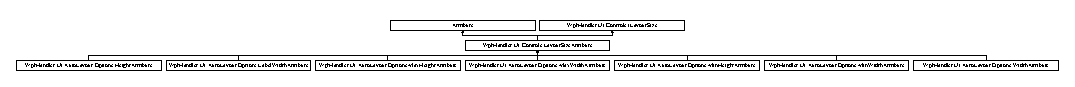
\includegraphics[height=0.727273cm]{d7/d51/class_wpf_handler_1_1_u_i_1_1_controls_1_1_layout_size_attribute}
\end{center}
\end{figure}
\subsection*{Public Member Functions}
\begin{DoxyCompactItemize}
\item 
\mbox{\hyperlink{class_wpf_handler_1_1_u_i_1_1_controls_1_1_layout_size_attribute_ade163e9b2952d02cda556e26bf6be52f}{Layout\+Size\+Attribute}} ()
\begin{DoxyCompactList}\small\item\em Default constructor. Use auto width. \end{DoxyCompactList}\item 
\mbox{\hyperlink{class_wpf_handler_1_1_u_i_1_1_controls_1_1_layout_size_attribute_a35d91131ec3931e5bde8cf3b026ff23c}{Layout\+Size\+Attribute}} (double width)
\begin{DoxyCompactList}\small\item\em Set requested width as Size. \end{DoxyCompactList}\end{DoxyCompactItemize}
\subsection*{Properties}
\begin{DoxyCompactItemize}
\item 
double \mbox{\hyperlink{class_wpf_handler_1_1_u_i_1_1_controls_1_1_layout_size_attribute_a3cf68aa208cfd09f789773f844683f87}{Size}} = double.\+NaN\hspace{0.3cm}{\ttfamily  \mbox{[}get, set\mbox{]}}
\begin{DoxyCompactList}\small\item\em Value that will be used in the element\textquotesingle{}s propeties. \end{DoxyCompactList}\end{DoxyCompactItemize}


\subsection{Detailed Description}
Attribute for managing layout size of some element. Provides base members. 



\subsection{Constructor \& Destructor Documentation}
\mbox{\Hypertarget{class_wpf_handler_1_1_u_i_1_1_controls_1_1_layout_size_attribute_ade163e9b2952d02cda556e26bf6be52f}\label{class_wpf_handler_1_1_u_i_1_1_controls_1_1_layout_size_attribute_ade163e9b2952d02cda556e26bf6be52f}} 
\index{Wpf\+Handler\+::\+U\+I\+::\+Controls\+::\+Layout\+Size\+Attribute@{Wpf\+Handler\+::\+U\+I\+::\+Controls\+::\+Layout\+Size\+Attribute}!Layout\+Size\+Attribute@{Layout\+Size\+Attribute}}
\index{Layout\+Size\+Attribute@{Layout\+Size\+Attribute}!Wpf\+Handler\+::\+U\+I\+::\+Controls\+::\+Layout\+Size\+Attribute@{Wpf\+Handler\+::\+U\+I\+::\+Controls\+::\+Layout\+Size\+Attribute}}
\subsubsection{\texorpdfstring{Layout\+Size\+Attribute()}{LayoutSizeAttribute()}\hspace{0.1cm}{\footnotesize\ttfamily [1/2]}}
{\footnotesize\ttfamily Wpf\+Handler.\+U\+I.\+Controls.\+Layout\+Size\+Attribute.\+Layout\+Size\+Attribute (\begin{DoxyParamCaption}{ }\end{DoxyParamCaption})}



Default constructor. Use auto width. 

\mbox{\Hypertarget{class_wpf_handler_1_1_u_i_1_1_controls_1_1_layout_size_attribute_a35d91131ec3931e5bde8cf3b026ff23c}\label{class_wpf_handler_1_1_u_i_1_1_controls_1_1_layout_size_attribute_a35d91131ec3931e5bde8cf3b026ff23c}} 
\index{Wpf\+Handler\+::\+U\+I\+::\+Controls\+::\+Layout\+Size\+Attribute@{Wpf\+Handler\+::\+U\+I\+::\+Controls\+::\+Layout\+Size\+Attribute}!Layout\+Size\+Attribute@{Layout\+Size\+Attribute}}
\index{Layout\+Size\+Attribute@{Layout\+Size\+Attribute}!Wpf\+Handler\+::\+U\+I\+::\+Controls\+::\+Layout\+Size\+Attribute@{Wpf\+Handler\+::\+U\+I\+::\+Controls\+::\+Layout\+Size\+Attribute}}
\subsubsection{\texorpdfstring{Layout\+Size\+Attribute()}{LayoutSizeAttribute()}\hspace{0.1cm}{\footnotesize\ttfamily [2/2]}}
{\footnotesize\ttfamily Wpf\+Handler.\+U\+I.\+Controls.\+Layout\+Size\+Attribute.\+Layout\+Size\+Attribute (\begin{DoxyParamCaption}\item[{double}]{width }\end{DoxyParamCaption})}



Set requested width as Size. 


\begin{DoxyParams}{Parameters}
{\em width} & \\
\hline
\end{DoxyParams}


\subsection{Property Documentation}
\mbox{\Hypertarget{class_wpf_handler_1_1_u_i_1_1_controls_1_1_layout_size_attribute_a3cf68aa208cfd09f789773f844683f87}\label{class_wpf_handler_1_1_u_i_1_1_controls_1_1_layout_size_attribute_a3cf68aa208cfd09f789773f844683f87}} 
\index{Wpf\+Handler\+::\+U\+I\+::\+Controls\+::\+Layout\+Size\+Attribute@{Wpf\+Handler\+::\+U\+I\+::\+Controls\+::\+Layout\+Size\+Attribute}!Size@{Size}}
\index{Size@{Size}!Wpf\+Handler\+::\+U\+I\+::\+Controls\+::\+Layout\+Size\+Attribute@{Wpf\+Handler\+::\+U\+I\+::\+Controls\+::\+Layout\+Size\+Attribute}}
\subsubsection{\texorpdfstring{Size}{Size}}
{\footnotesize\ttfamily double Wpf\+Handler.\+U\+I.\+Controls.\+Layout\+Size\+Attribute.\+Size = double.\+NaN\hspace{0.3cm}{\ttfamily [get]}, {\ttfamily [set]}}



Value that will be used in the element\textquotesingle{}s propeties. 



The documentation for this class was generated from the following file\+:\begin{DoxyCompactItemize}
\item 
D\+:/\+Work/\+Git\+Hub/wpf-\/handler/\+Wpf\+Handler/\+U\+I/\+Controls/Layout\+Size\+Attribute.\+cs\end{DoxyCompactItemize}

\hypertarget{class_wpf_handler_1_1_dictionaries_1_1_localizable_content_attribute}{}\section{Wpf\+Handler.\+Dictionaries.\+Localizable\+Content\+Attribute Class Reference}
\label{class_wpf_handler_1_1_dictionaries_1_1_localizable_content_attribute}\index{Wpf\+Handler.\+Dictionaries.\+Localizable\+Content\+Attribute@{Wpf\+Handler.\+Dictionaries.\+Localizable\+Content\+Attribute}}


Base attribute that binding \mbox{\hyperlink{namespace_wpf_handler_1_1_u_i}{UI}} element to the common auto localization system.  


Inheritance diagram for Wpf\+Handler.\+Dictionaries.\+Localizable\+Content\+Attribute\+:\begin{figure}[H]
\begin{center}
\leavevmode
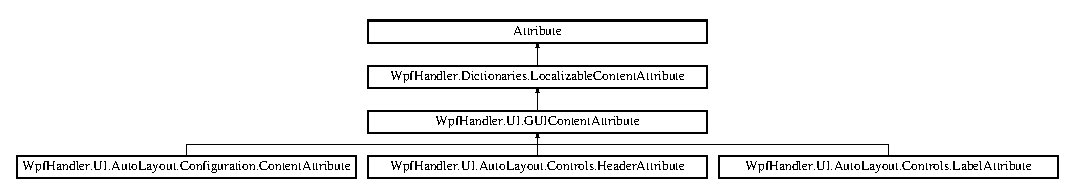
\includegraphics[height=2.170543cm]{db/dbf/class_wpf_handler_1_1_dictionaries_1_1_localizable_content_attribute}
\end{center}
\end{figure}
\subsection*{Public Member Functions}
\begin{DoxyCompactItemize}
\item 
\mbox{\hyperlink{class_wpf_handler_1_1_dictionaries_1_1_localizable_content_attribute_abba3c6699a97cc5a417eebc194979acd}{Localizable\+Content\+Attribute}} ()
\begin{DoxyCompactList}\small\item\em Default constructor. \end{DoxyCompactList}\item 
abstract void \mbox{\hyperlink{class_wpf_handler_1_1_dictionaries_1_1_localizable_content_attribute_a001e110c7ad42422bc02a44d9eedc801}{Languages\+Dictionaries\+Updated}} ()
\begin{DoxyCompactList}\small\item\em Occurs when would reloaded dynamic dictionaries. \end{DoxyCompactList}\end{DoxyCompactItemize}
\subsection*{Private Member Functions}
\begin{DoxyCompactItemize}
\item 
\mbox{\hyperlink{class_wpf_handler_1_1_dictionaries_1_1_localizable_content_attribute_a38a1f37df12d6f6205ab32933ddeb5b1}{$\sim$\+Localizable\+Content\+Attribute}} ()
\begin{DoxyCompactList}\small\item\em Unsubscribe from events. \end{DoxyCompactList}\end{DoxyCompactItemize}


\subsection{Detailed Description}
Base attribute that binding \mbox{\hyperlink{namespace_wpf_handler_1_1_u_i}{UI}} element to the common auto localization system. 



\subsection{Constructor \& Destructor Documentation}
\mbox{\Hypertarget{class_wpf_handler_1_1_dictionaries_1_1_localizable_content_attribute_abba3c6699a97cc5a417eebc194979acd}\label{class_wpf_handler_1_1_dictionaries_1_1_localizable_content_attribute_abba3c6699a97cc5a417eebc194979acd}} 
\index{Wpf\+Handler\+::\+Dictionaries\+::\+Localizable\+Content\+Attribute@{Wpf\+Handler\+::\+Dictionaries\+::\+Localizable\+Content\+Attribute}!Localizable\+Content\+Attribute@{Localizable\+Content\+Attribute}}
\index{Localizable\+Content\+Attribute@{Localizable\+Content\+Attribute}!Wpf\+Handler\+::\+Dictionaries\+::\+Localizable\+Content\+Attribute@{Wpf\+Handler\+::\+Dictionaries\+::\+Localizable\+Content\+Attribute}}
\subsubsection{\texorpdfstring{Localizable\+Content\+Attribute()}{LocalizableContentAttribute()}}
{\footnotesize\ttfamily Wpf\+Handler.\+Dictionaries.\+Localizable\+Content\+Attribute.\+Localizable\+Content\+Attribute (\begin{DoxyParamCaption}{ }\end{DoxyParamCaption})}



Default constructor. 

\mbox{\Hypertarget{class_wpf_handler_1_1_dictionaries_1_1_localizable_content_attribute_a38a1f37df12d6f6205ab32933ddeb5b1}\label{class_wpf_handler_1_1_dictionaries_1_1_localizable_content_attribute_a38a1f37df12d6f6205ab32933ddeb5b1}} 
\index{Wpf\+Handler\+::\+Dictionaries\+::\+Localizable\+Content\+Attribute@{Wpf\+Handler\+::\+Dictionaries\+::\+Localizable\+Content\+Attribute}!````~Localizable\+Content\+Attribute@{$\sim$\+Localizable\+Content\+Attribute}}
\index{````~Localizable\+Content\+Attribute@{$\sim$\+Localizable\+Content\+Attribute}!Wpf\+Handler\+::\+Dictionaries\+::\+Localizable\+Content\+Attribute@{Wpf\+Handler\+::\+Dictionaries\+::\+Localizable\+Content\+Attribute}}
\subsubsection{\texorpdfstring{$\sim$\+Localizable\+Content\+Attribute()}{~LocalizableContentAttribute()}}
{\footnotesize\ttfamily Wpf\+Handler.\+Dictionaries.\+Localizable\+Content\+Attribute.$\sim$\+Localizable\+Content\+Attribute (\begin{DoxyParamCaption}{ }\end{DoxyParamCaption})\hspace{0.3cm}{\ttfamily [private]}}



Unsubscribe from events. 



\subsection{Member Function Documentation}
\mbox{\Hypertarget{class_wpf_handler_1_1_dictionaries_1_1_localizable_content_attribute_a001e110c7ad42422bc02a44d9eedc801}\label{class_wpf_handler_1_1_dictionaries_1_1_localizable_content_attribute_a001e110c7ad42422bc02a44d9eedc801}} 
\index{Wpf\+Handler\+::\+Dictionaries\+::\+Localizable\+Content\+Attribute@{Wpf\+Handler\+::\+Dictionaries\+::\+Localizable\+Content\+Attribute}!Languages\+Dictionaries\+Updated@{Languages\+Dictionaries\+Updated}}
\index{Languages\+Dictionaries\+Updated@{Languages\+Dictionaries\+Updated}!Wpf\+Handler\+::\+Dictionaries\+::\+Localizable\+Content\+Attribute@{Wpf\+Handler\+::\+Dictionaries\+::\+Localizable\+Content\+Attribute}}
\subsubsection{\texorpdfstring{Languages\+Dictionaries\+Updated()}{LanguagesDictionariesUpdated()}}
{\footnotesize\ttfamily abstract void Wpf\+Handler.\+Dictionaries.\+Localizable\+Content\+Attribute.\+Languages\+Dictionaries\+Updated (\begin{DoxyParamCaption}{ }\end{DoxyParamCaption})\hspace{0.3cm}{\ttfamily [pure virtual]}}



Occurs when would reloaded dynamic dictionaries. 



Implemented in \mbox{\hyperlink{class_wpf_handler_1_1_u_i_1_1_auto_layout_1_1_controls_1_1_header_attribute_ae2587a69606cda16cc87e901140f113a}{Wpf\+Handler.\+U\+I.\+Auto\+Layout.\+Controls.\+Header\+Attribute}}, \mbox{\hyperlink{class_wpf_handler_1_1_u_i_1_1_auto_layout_1_1_configuration_1_1_content_attribute_a498818bc121b7f408af302eb4085056a}{Wpf\+Handler.\+U\+I.\+Auto\+Layout.\+Configuration.\+Content\+Attribute}}, and \mbox{\hyperlink{class_wpf_handler_1_1_u_i_1_1_auto_layout_1_1_controls_1_1_label_attribute_a3ed5f61dc946ffd5ce385cc4ef60362d}{Wpf\+Handler.\+U\+I.\+Auto\+Layout.\+Controls.\+Label\+Attribute}}.



The documentation for this class was generated from the following file\+:\begin{DoxyCompactItemize}
\item 
D\+:/\+Work/\+Git\+Hub/wpf-\/handler/\+Wpf\+Handler/\+Dictionaries/Localizable\+Content\+Attribute.\+cs\end{DoxyCompactItemize}

\hypertarget{class_wpf_handler_1_1_u_i_1_1_localization_handler}{}\section{Wpf\+Handler.\+U\+I.\+Localization\+Handler Class Reference}
\label{class_wpf_handler_1_1_u_i_1_1_localization_handler}\index{Wpf\+Handler.\+U\+I.\+Localization\+Handler@{Wpf\+Handler.\+U\+I.\+Localization\+Handler}}


Provides the A\+PI to managing the localization system.  


\subsection*{Static Public Member Functions}
\begin{DoxyCompactItemize}
\item 
static void \mbox{\hyperlink{class_wpf_handler_1_1_u_i_1_1_localization_handler_a619201b52fa3480e4bdb75231ebdd666}{Bind\+To\+Label}} (this \mbox{\hyperlink{class_wpf_handler_1_1_u_i_1_1_g_u_i_content}{G\+U\+I\+Content}} content, \mbox{\hyperlink{interface_wpf_handler_1_1_u_i_1_1_controls_1_1_i_label}{I\+Label}} label)
\begin{DoxyCompactList}\small\item\em Connecting instiniated control with label to localization updates. \end{DoxyCompactList}\item 
static void \mbox{\hyperlink{class_wpf_handler_1_1_u_i_1_1_localization_handler_a45a3a6581764446bf67a622119d9b89d}{Bind\+To\+Label}} (this \mbox{\hyperlink{class_wpf_handler_1_1_u_i_1_1_g_u_i_content}{G\+U\+I\+Content}} content, \mbox{\hyperlink{interface_wpf_handler_1_1_u_i_1_1_controls_1_1_i_label}{I\+Label}} label, Member\+Info source\+Member)
\begin{DoxyCompactList}\small\item\em Connecting instiniated control with label to localization updates. \end{DoxyCompactList}\item 
static void \mbox{\hyperlink{class_wpf_handler_1_1_u_i_1_1_localization_handler_a8159e214fd8c0709f32b5b1b3cf25020}{Load\+Dictionaries}} (params Culture\+Info\mbox{[}$\,$\mbox{]} cultures\+Order)
\begin{DoxyCompactList}\small\item\em Scaning for language dictionaries in X\+A\+ML files stored by \mbox{\hyperlink{class_wpf_handler_1_1_plugins_1_1_constants_a96f55ef86fe92a534722f4788340f390}{Plugins.\+Constants.\+P\+L\+U\+G\+I\+N\+S\+\_\+\+D\+IR}}, and loading them to Merged dictionaries. Loading only relative to the new culture if found. Leave a previous culture if not. \end{DoxyCompactList}\item 
static void \mbox{\hyperlink{class_wpf_handler_1_1_u_i_1_1_localization_handler_a5703a690547759b592d63b5f5b2f489e}{Unload\+Dictionaries}} ()
\begin{DoxyCompactList}\small\item\em Unloading all current loaded localization dictionaries. \end{DoxyCompactList}\end{DoxyCompactItemize}
\subsection*{Events}
\begin{DoxyCompactItemize}
\item 
static Action \mbox{\hyperlink{class_wpf_handler_1_1_u_i_1_1_localization_handler_afa222c8723785db39e70a9694e2e5398}{Languages\+Dictionaries\+Updated}}
\begin{DoxyCompactList}\small\item\em Event that occurs when languages dictionary will be loaded. \end{DoxyCompactList}\end{DoxyCompactItemize}


\subsection{Detailed Description}
Provides the A\+PI to managing the localization system. 



\subsection{Member Function Documentation}
\mbox{\Hypertarget{class_wpf_handler_1_1_u_i_1_1_localization_handler_a619201b52fa3480e4bdb75231ebdd666}\label{class_wpf_handler_1_1_u_i_1_1_localization_handler_a619201b52fa3480e4bdb75231ebdd666}} 
\index{Wpf\+Handler\+::\+U\+I\+::\+Localization\+Handler@{Wpf\+Handler\+::\+U\+I\+::\+Localization\+Handler}!Bind\+To\+Label@{Bind\+To\+Label}}
\index{Bind\+To\+Label@{Bind\+To\+Label}!Wpf\+Handler\+::\+U\+I\+::\+Localization\+Handler@{Wpf\+Handler\+::\+U\+I\+::\+Localization\+Handler}}
\subsubsection{\texorpdfstring{Bind\+To\+Label()}{BindToLabel()}\hspace{0.1cm}{\footnotesize\ttfamily [1/2]}}
{\footnotesize\ttfamily static void Wpf\+Handler.\+U\+I.\+Localization\+Handler.\+Bind\+To\+Label (\begin{DoxyParamCaption}\item[{this \mbox{\hyperlink{class_wpf_handler_1_1_u_i_1_1_g_u_i_content}{G\+U\+I\+Content}}}]{content,  }\item[{\mbox{\hyperlink{interface_wpf_handler_1_1_u_i_1_1_controls_1_1_i_label}{I\+Label}}}]{label }\end{DoxyParamCaption})\hspace{0.3cm}{\ttfamily [static]}}



Connecting instiniated control with label to localization updates. 


\begin{DoxyParams}{Parameters}
{\em content} & Content handler that will manage the label.\\
\hline
{\em label} & \mbox{\hyperlink{namespace_wpf_handler_1_1_u_i}{UI}} control that has a label to content bridging.\\
\hline
\end{DoxyParams}
\mbox{\Hypertarget{class_wpf_handler_1_1_u_i_1_1_localization_handler_a45a3a6581764446bf67a622119d9b89d}\label{class_wpf_handler_1_1_u_i_1_1_localization_handler_a45a3a6581764446bf67a622119d9b89d}} 
\index{Wpf\+Handler\+::\+U\+I\+::\+Localization\+Handler@{Wpf\+Handler\+::\+U\+I\+::\+Localization\+Handler}!Bind\+To\+Label@{Bind\+To\+Label}}
\index{Bind\+To\+Label@{Bind\+To\+Label}!Wpf\+Handler\+::\+U\+I\+::\+Localization\+Handler@{Wpf\+Handler\+::\+U\+I\+::\+Localization\+Handler}}
\subsubsection{\texorpdfstring{Bind\+To\+Label()}{BindToLabel()}\hspace{0.1cm}{\footnotesize\ttfamily [2/2]}}
{\footnotesize\ttfamily static void Wpf\+Handler.\+U\+I.\+Localization\+Handler.\+Bind\+To\+Label (\begin{DoxyParamCaption}\item[{this \mbox{\hyperlink{class_wpf_handler_1_1_u_i_1_1_g_u_i_content}{G\+U\+I\+Content}}}]{content,  }\item[{\mbox{\hyperlink{interface_wpf_handler_1_1_u_i_1_1_controls_1_1_i_label}{I\+Label}}}]{label,  }\item[{Member\+Info}]{source\+Member }\end{DoxyParamCaption})\hspace{0.3cm}{\ttfamily [static]}}



Connecting instiniated control with label to localization updates. 


\begin{DoxyParams}{Parameters}
{\em content} & Content handler that will manage the label.\\
\hline
{\em label} & \mbox{\hyperlink{namespace_wpf_handler_1_1_u_i}{UI}} control that has a label to content bridging.\\
\hline
{\em source\+Member} & Member infor that could be used as source for auto generated title in case if \mbox{\hyperlink{class_wpf_handler_1_1_u_i_1_1_g_u_i_content}{G\+U\+I\+Content}} not provided in resources.\\
\hline
\end{DoxyParams}
\mbox{\Hypertarget{class_wpf_handler_1_1_u_i_1_1_localization_handler_a8159e214fd8c0709f32b5b1b3cf25020}\label{class_wpf_handler_1_1_u_i_1_1_localization_handler_a8159e214fd8c0709f32b5b1b3cf25020}} 
\index{Wpf\+Handler\+::\+U\+I\+::\+Localization\+Handler@{Wpf\+Handler\+::\+U\+I\+::\+Localization\+Handler}!Load\+Dictionaries@{Load\+Dictionaries}}
\index{Load\+Dictionaries@{Load\+Dictionaries}!Wpf\+Handler\+::\+U\+I\+::\+Localization\+Handler@{Wpf\+Handler\+::\+U\+I\+::\+Localization\+Handler}}
\subsubsection{\texorpdfstring{Load\+Dictionaries()}{LoadDictionaries()}}
{\footnotesize\ttfamily static void Wpf\+Handler.\+U\+I.\+Localization\+Handler.\+Load\+Dictionaries (\begin{DoxyParamCaption}\item[{params Culture\+Info \mbox{[}$\,$\mbox{]}}]{cultures\+Order }\end{DoxyParamCaption})\hspace{0.3cm}{\ttfamily [static]}}



Scaning for language dictionaries in X\+A\+ML files stored by \mbox{\hyperlink{class_wpf_handler_1_1_plugins_1_1_constants_a96f55ef86fe92a534722f4788340f390}{Plugins.\+Constants.\+P\+L\+U\+G\+I\+N\+S\+\_\+\+D\+IR}}, and loading them to Merged dictionaries. Loading only relative to the new culture if found. Leave a previous culture if not. 

Require files format\+: $\ast$.lang.\+C\+U\+L\+T\+U\+R\+E\+\_\+\+C\+O\+D\+E.\+xaml, where culture code equal current translation of the app. Example\+: plugin.\+feed.\+lang.\+en-\/\+U\+S.\+xaml 


\begin{DoxyParams}{Parameters}
{\em cultures\+Order} & Array of cultures reuested to loading in the priiority oreder.\\
\hline
\end{DoxyParams}
\mbox{\Hypertarget{class_wpf_handler_1_1_u_i_1_1_localization_handler_a5703a690547759b592d63b5f5b2f489e}\label{class_wpf_handler_1_1_u_i_1_1_localization_handler_a5703a690547759b592d63b5f5b2f489e}} 
\index{Wpf\+Handler\+::\+U\+I\+::\+Localization\+Handler@{Wpf\+Handler\+::\+U\+I\+::\+Localization\+Handler}!Unload\+Dictionaries@{Unload\+Dictionaries}}
\index{Unload\+Dictionaries@{Unload\+Dictionaries}!Wpf\+Handler\+::\+U\+I\+::\+Localization\+Handler@{Wpf\+Handler\+::\+U\+I\+::\+Localization\+Handler}}
\subsubsection{\texorpdfstring{Unload\+Dictionaries()}{UnloadDictionaries()}}
{\footnotesize\ttfamily static void Wpf\+Handler.\+U\+I.\+Localization\+Handler.\+Unload\+Dictionaries (\begin{DoxyParamCaption}{ }\end{DoxyParamCaption})\hspace{0.3cm}{\ttfamily [static]}}



Unloading all current loaded localization dictionaries. 



\subsection{Event Documentation}
\mbox{\Hypertarget{class_wpf_handler_1_1_u_i_1_1_localization_handler_afa222c8723785db39e70a9694e2e5398}\label{class_wpf_handler_1_1_u_i_1_1_localization_handler_afa222c8723785db39e70a9694e2e5398}} 
\index{Wpf\+Handler\+::\+U\+I\+::\+Localization\+Handler@{Wpf\+Handler\+::\+U\+I\+::\+Localization\+Handler}!Languages\+Dictionaries\+Updated@{Languages\+Dictionaries\+Updated}}
\index{Languages\+Dictionaries\+Updated@{Languages\+Dictionaries\+Updated}!Wpf\+Handler\+::\+U\+I\+::\+Localization\+Handler@{Wpf\+Handler\+::\+U\+I\+::\+Localization\+Handler}}
\subsubsection{\texorpdfstring{Languages\+Dictionaries\+Updated}{LanguagesDictionariesUpdated}}
{\footnotesize\ttfamily Action Wpf\+Handler.\+U\+I.\+Localization\+Handler.\+Languages\+Dictionaries\+Updated\hspace{0.3cm}{\ttfamily [static]}}



Event that occurs when languages dictionary will be loaded. 



The documentation for this class was generated from the following file\+:\begin{DoxyCompactItemize}
\item 
D\+:/\+Work/\+Git\+Hub/wpf-\/handler/\+Wpf\+Handler/\+U\+I/Localization\+Handler.\+cs\end{DoxyCompactItemize}

\hypertarget{class_wpf_handler_1_1_u_i_1_1_controls_1_1_lock_screen}{}\section{Wpf\+Handler.\+U\+I.\+Controls.\+Lock\+Screen Class Reference}
\label{class_wpf_handler_1_1_u_i_1_1_controls_1_1_lock_screen}\index{Wpf\+Handler.\+U\+I.\+Controls.\+Lock\+Screen@{Wpf\+Handler.\+U\+I.\+Controls.\+Lock\+Screen}}


\mbox{\hyperlink{class_wpf_handler_1_1_u_i_1_1_controls_1_1_lock_screen}{Lock\+Screen}}  


Inheritance diagram for Wpf\+Handler.\+U\+I.\+Controls.\+Lock\+Screen\+:\begin{figure}[H]
\begin{center}
\leavevmode
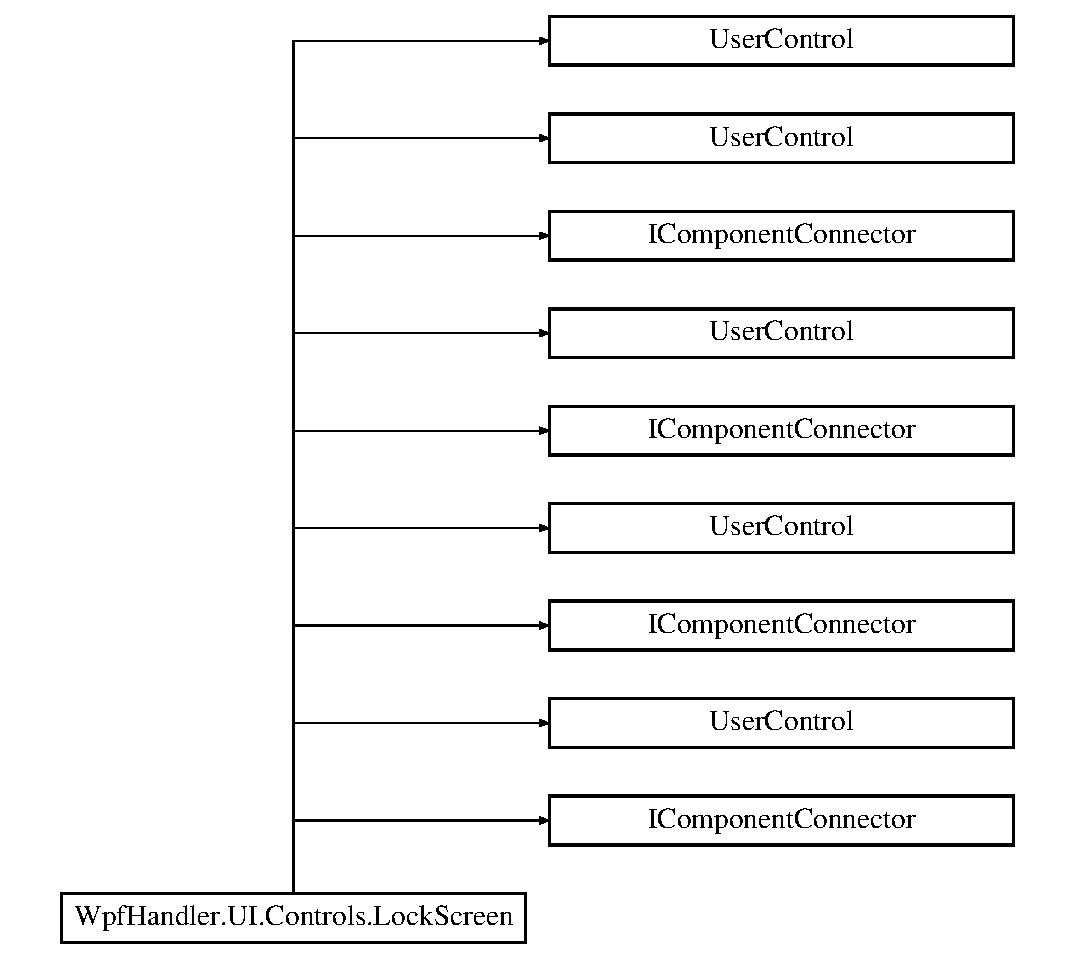
\includegraphics[height=10.000000cm]{dc/d68/class_wpf_handler_1_1_u_i_1_1_controls_1_1_lock_screen}
\end{center}
\end{figure}
\subsection*{Public Member Functions}
\begin{DoxyCompactItemize}
\item 
void \mbox{\hyperlink{class_wpf_handler_1_1_u_i_1_1_controls_1_1_lock_screen_aacd97a7da29eefb57cc695f5af31dce5}{Initialize\+Component}} ()
\begin{DoxyCompactList}\small\item\em Initialize\+Component \end{DoxyCompactList}\item 
void \mbox{\hyperlink{class_wpf_handler_1_1_u_i_1_1_controls_1_1_lock_screen_aacd97a7da29eefb57cc695f5af31dce5}{Initialize\+Component}} ()
\begin{DoxyCompactList}\small\item\em Initialize\+Component \end{DoxyCompactList}\item 
void \mbox{\hyperlink{class_wpf_handler_1_1_u_i_1_1_controls_1_1_lock_screen_aacd97a7da29eefb57cc695f5af31dce5}{Initialize\+Component}} ()
\begin{DoxyCompactList}\small\item\em Initialize\+Component \end{DoxyCompactList}\item 
void \mbox{\hyperlink{class_wpf_handler_1_1_u_i_1_1_controls_1_1_lock_screen_aacd97a7da29eefb57cc695f5af31dce5}{Initialize\+Component}} ()
\begin{DoxyCompactList}\small\item\em Initialize\+Component \end{DoxyCompactList}\item 
\mbox{\hyperlink{class_wpf_handler_1_1_u_i_1_1_controls_1_1_lock_screen_a9b03e106f5477ce912a76c7b7de5aac2}{Lock\+Screen}} ()
\begin{DoxyCompactList}\small\item\em Default constructor. \end{DoxyCompactList}\item 
void \mbox{\hyperlink{class_wpf_handler_1_1_u_i_1_1_controls_1_1_lock_screen_ae53cb9098b105a55f6da81acf3703e69}{Lock}} (string message, params Framework\+Element\mbox{[}$\,$\mbox{]} controls)
\begin{DoxyCompactList}\small\item\em Lock screen and enable loading animation. \end{DoxyCompactList}\item 
void \mbox{\hyperlink{class_wpf_handler_1_1_u_i_1_1_controls_1_1_lock_screen_a2411f98b2544601d6310967dc93064a2}{Unlock}} ()
\begin{DoxyCompactList}\small\item\em Unlock screen. \end{DoxyCompactList}\item 
void \mbox{\hyperlink{class_wpf_handler_1_1_u_i_1_1_controls_1_1_lock_screen_ab3d0b280c769a2c9ed57766d03791fd7}{Lock\+Cancel\+Callback\+Handler}} (object sender, Routed\+Event\+Args args)
\begin{DoxyCompactList}\small\item\em Occurs when lock screee cancel button is pressed. \end{DoxyCompactList}\end{DoxyCompactItemize}
\subsection*{Public Attributes}
\begin{DoxyCompactItemize}
\item 
Time\+Span \mbox{\hyperlink{class_wpf_handler_1_1_u_i_1_1_controls_1_1_lock_screen_aa2733098fb7a92be1c98a6b0ac47972c}{lock\+Animation\+Duration}} = new Time\+Span(0, 0, 0, 0, 300)
\begin{DoxyCompactList}\small\item\em How many time will take blur animation. \end{DoxyCompactList}\item 
float \mbox{\hyperlink{class_wpf_handler_1_1_u_i_1_1_controls_1_1_lock_screen_a5152e45504e88316e8d76753577ea4b5}{blur\+Size}} = 20
\begin{DoxyCompactList}\small\item\em Size of Gausian blur. \end{DoxyCompactList}\end{DoxyCompactItemize}
\subsection*{Protected Attributes}
\begin{DoxyCompactItemize}
\item 
Framework\+Element \mbox{[}$\,$\mbox{]} \mbox{\hyperlink{class_wpf_handler_1_1_u_i_1_1_controls_1_1_lock_screen_a6c0e4649ba3a27b7e55d32ddf093d4dd}{locked\+Ellements}}
\begin{DoxyCompactList}\small\item\em Elements that would locked. \end{DoxyCompactList}\end{DoxyCompactItemize}
\subsection*{Package Functions}
\begin{DoxyCompactItemize}
\item 
\mbox{\Hypertarget{class_wpf_handler_1_1_u_i_1_1_controls_1_1_lock_screen_aeadd163b71840ecd0f5364997bf4dd49}\label{class_wpf_handler_1_1_u_i_1_1_controls_1_1_lock_screen_aeadd163b71840ecd0f5364997bf4dd49}} 
System.\+Delegate {\bfseries \+\_\+\+Create\+Delegate} (System.\+Type delegate\+Type, string handler)
\item 
\mbox{\Hypertarget{class_wpf_handler_1_1_u_i_1_1_controls_1_1_lock_screen_aeadd163b71840ecd0f5364997bf4dd49}\label{class_wpf_handler_1_1_u_i_1_1_controls_1_1_lock_screen_aeadd163b71840ecd0f5364997bf4dd49}} 
System.\+Delegate {\bfseries \+\_\+\+Create\+Delegate} (System.\+Type delegate\+Type, string handler)
\item 
\mbox{\Hypertarget{class_wpf_handler_1_1_u_i_1_1_controls_1_1_lock_screen_aeadd163b71840ecd0f5364997bf4dd49}\label{class_wpf_handler_1_1_u_i_1_1_controls_1_1_lock_screen_aeadd163b71840ecd0f5364997bf4dd49}} 
System.\+Delegate {\bfseries \+\_\+\+Create\+Delegate} (System.\+Type delegate\+Type, string handler)
\item 
\mbox{\Hypertarget{class_wpf_handler_1_1_u_i_1_1_controls_1_1_lock_screen_aeadd163b71840ecd0f5364997bf4dd49}\label{class_wpf_handler_1_1_u_i_1_1_controls_1_1_lock_screen_aeadd163b71840ecd0f5364997bf4dd49}} 
System.\+Delegate {\bfseries \+\_\+\+Create\+Delegate} (System.\+Type delegate\+Type, string handler)
\end{DoxyCompactItemize}
\subsection*{Package Attributes}
\begin{DoxyCompactItemize}
\item 
\mbox{\Hypertarget{class_wpf_handler_1_1_u_i_1_1_controls_1_1_lock_screen_a70df15cf031c4b8b17660091f35eaf5c}\label{class_wpf_handler_1_1_u_i_1_1_controls_1_1_lock_screen_a70df15cf031c4b8b17660091f35eaf5c}} 
System.\+Windows.\+Controls.\+Grid {\bfseries lock\+Screen}
\item 
\mbox{\Hypertarget{class_wpf_handler_1_1_u_i_1_1_controls_1_1_lock_screen_a567f1855147e8635ebd8980dc6da744b}\label{class_wpf_handler_1_1_u_i_1_1_controls_1_1_lock_screen_a567f1855147e8635ebd8980dc6da744b}} 
System.\+Windows.\+Controls.\+Grid {\bfseries backplate}
\item 
\mbox{\Hypertarget{class_wpf_handler_1_1_u_i_1_1_controls_1_1_lock_screen_a0bc49ea590c0e024d2d6fa2ee6bff68c}\label{class_wpf_handler_1_1_u_i_1_1_controls_1_1_lock_screen_a0bc49ea590c0e024d2d6fa2ee6bff68c}} 
System.\+Windows.\+Controls.\+Label {\bfseries lock\+Label}
\item 
\mbox{\Hypertarget{class_wpf_handler_1_1_u_i_1_1_controls_1_1_lock_screen_a685dc9d63cfe051b2dd651d474402163}\label{class_wpf_handler_1_1_u_i_1_1_controls_1_1_lock_screen_a685dc9d63cfe051b2dd651d474402163}} 
\mbox{\hyperlink{class_wpf_handler_1_1_u_i_1_1_controls_1_1_flat_button}{Wpf\+Handler.\+U\+I.\+Controls.\+Flat\+Button}} {\bfseries lock\+Cancel\+Button}
\end{DoxyCompactItemize}
\subsection*{Properties}
\begin{DoxyCompactItemize}
\item 
Action$<$ object $>$ \mbox{\hyperlink{class_wpf_handler_1_1_u_i_1_1_controls_1_1_lock_screen_a43e0275f123b6e3d5dcf2f9032a67e82}{Operation\+Cancel\+Callback}}\hspace{0.3cm}{\ttfamily  \mbox{[}get, set\mbox{]}}
\begin{DoxyCompactList}\small\item\em Method that will has been calling during click on operation cancel button. \end{DoxyCompactList}\end{DoxyCompactItemize}
\subsection*{Private Member Functions}
\begin{DoxyCompactItemize}
\item 
\mbox{\Hypertarget{class_wpf_handler_1_1_u_i_1_1_controls_1_1_lock_screen_a0f64872e36d05d04de460b1a0adf7e2d}\label{class_wpf_handler_1_1_u_i_1_1_controls_1_1_lock_screen_a0f64872e36d05d04de460b1a0adf7e2d}} 
void System.\+Windows.\+Markup.\+I\+Component\+Connector. {\bfseries Connect} (int connection\+Id, object target)
\item 
\mbox{\Hypertarget{class_wpf_handler_1_1_u_i_1_1_controls_1_1_lock_screen_a0f64872e36d05d04de460b1a0adf7e2d}\label{class_wpf_handler_1_1_u_i_1_1_controls_1_1_lock_screen_a0f64872e36d05d04de460b1a0adf7e2d}} 
void System.\+Windows.\+Markup.\+I\+Component\+Connector. {\bfseries Connect} (int connection\+Id, object target)
\item 
\mbox{\Hypertarget{class_wpf_handler_1_1_u_i_1_1_controls_1_1_lock_screen_a0f64872e36d05d04de460b1a0adf7e2d}\label{class_wpf_handler_1_1_u_i_1_1_controls_1_1_lock_screen_a0f64872e36d05d04de460b1a0adf7e2d}} 
void System.\+Windows.\+Markup.\+I\+Component\+Connector. {\bfseries Connect} (int connection\+Id, object target)
\item 
\mbox{\Hypertarget{class_wpf_handler_1_1_u_i_1_1_controls_1_1_lock_screen_a0f64872e36d05d04de460b1a0adf7e2d}\label{class_wpf_handler_1_1_u_i_1_1_controls_1_1_lock_screen_a0f64872e36d05d04de460b1a0adf7e2d}} 
void System.\+Windows.\+Markup.\+I\+Component\+Connector. {\bfseries Connect} (int connection\+Id, object target)
\end{DoxyCompactItemize}
\subsection*{Private Attributes}
\begin{DoxyCompactItemize}
\item 
\mbox{\Hypertarget{class_wpf_handler_1_1_u_i_1_1_controls_1_1_lock_screen_a3e5cc93c865f07f3ce73d948bd43fb75}\label{class_wpf_handler_1_1_u_i_1_1_controls_1_1_lock_screen_a3e5cc93c865f07f3ce73d948bd43fb75}} 
bool {\bfseries \+\_\+content\+Loaded}
\end{DoxyCompactItemize}


\subsection{Detailed Description}
\mbox{\hyperlink{class_wpf_handler_1_1_u_i_1_1_controls_1_1_lock_screen}{Lock\+Screen}} 

Interaction logic for Lock\+Screen.\+xaml 

\subsection{Constructor \& Destructor Documentation}
\mbox{\Hypertarget{class_wpf_handler_1_1_u_i_1_1_controls_1_1_lock_screen_a9b03e106f5477ce912a76c7b7de5aac2}\label{class_wpf_handler_1_1_u_i_1_1_controls_1_1_lock_screen_a9b03e106f5477ce912a76c7b7de5aac2}} 
\index{Wpf\+Handler\+::\+U\+I\+::\+Controls\+::\+Lock\+Screen@{Wpf\+Handler\+::\+U\+I\+::\+Controls\+::\+Lock\+Screen}!Lock\+Screen@{Lock\+Screen}}
\index{Lock\+Screen@{Lock\+Screen}!Wpf\+Handler\+::\+U\+I\+::\+Controls\+::\+Lock\+Screen@{Wpf\+Handler\+::\+U\+I\+::\+Controls\+::\+Lock\+Screen}}
\subsubsection{\texorpdfstring{Lock\+Screen()}{LockScreen()}}
{\footnotesize\ttfamily Wpf\+Handler.\+U\+I.\+Controls.\+Lock\+Screen.\+Lock\+Screen (\begin{DoxyParamCaption}{ }\end{DoxyParamCaption})}



Default constructor. 



\subsection{Member Function Documentation}
\mbox{\Hypertarget{class_wpf_handler_1_1_u_i_1_1_controls_1_1_lock_screen_aacd97a7da29eefb57cc695f5af31dce5}\label{class_wpf_handler_1_1_u_i_1_1_controls_1_1_lock_screen_aacd97a7da29eefb57cc695f5af31dce5}} 
\index{Wpf\+Handler\+::\+U\+I\+::\+Controls\+::\+Lock\+Screen@{Wpf\+Handler\+::\+U\+I\+::\+Controls\+::\+Lock\+Screen}!Initialize\+Component@{Initialize\+Component}}
\index{Initialize\+Component@{Initialize\+Component}!Wpf\+Handler\+::\+U\+I\+::\+Controls\+::\+Lock\+Screen@{Wpf\+Handler\+::\+U\+I\+::\+Controls\+::\+Lock\+Screen}}
\subsubsection{\texorpdfstring{Initialize\+Component()}{InitializeComponent()}\hspace{0.1cm}{\footnotesize\ttfamily [1/4]}}
{\footnotesize\ttfamily void Wpf\+Handler.\+U\+I.\+Controls.\+Lock\+Screen.\+Initialize\+Component (\begin{DoxyParamCaption}{ }\end{DoxyParamCaption})}



Initialize\+Component 

\mbox{\Hypertarget{class_wpf_handler_1_1_u_i_1_1_controls_1_1_lock_screen_aacd97a7da29eefb57cc695f5af31dce5}\label{class_wpf_handler_1_1_u_i_1_1_controls_1_1_lock_screen_aacd97a7da29eefb57cc695f5af31dce5}} 
\index{Wpf\+Handler\+::\+U\+I\+::\+Controls\+::\+Lock\+Screen@{Wpf\+Handler\+::\+U\+I\+::\+Controls\+::\+Lock\+Screen}!Initialize\+Component@{Initialize\+Component}}
\index{Initialize\+Component@{Initialize\+Component}!Wpf\+Handler\+::\+U\+I\+::\+Controls\+::\+Lock\+Screen@{Wpf\+Handler\+::\+U\+I\+::\+Controls\+::\+Lock\+Screen}}
\subsubsection{\texorpdfstring{Initialize\+Component()}{InitializeComponent()}\hspace{0.1cm}{\footnotesize\ttfamily [2/4]}}
{\footnotesize\ttfamily void Wpf\+Handler.\+U\+I.\+Controls.\+Lock\+Screen.\+Initialize\+Component (\begin{DoxyParamCaption}{ }\end{DoxyParamCaption})}



Initialize\+Component 

\mbox{\Hypertarget{class_wpf_handler_1_1_u_i_1_1_controls_1_1_lock_screen_aacd97a7da29eefb57cc695f5af31dce5}\label{class_wpf_handler_1_1_u_i_1_1_controls_1_1_lock_screen_aacd97a7da29eefb57cc695f5af31dce5}} 
\index{Wpf\+Handler\+::\+U\+I\+::\+Controls\+::\+Lock\+Screen@{Wpf\+Handler\+::\+U\+I\+::\+Controls\+::\+Lock\+Screen}!Initialize\+Component@{Initialize\+Component}}
\index{Initialize\+Component@{Initialize\+Component}!Wpf\+Handler\+::\+U\+I\+::\+Controls\+::\+Lock\+Screen@{Wpf\+Handler\+::\+U\+I\+::\+Controls\+::\+Lock\+Screen}}
\subsubsection{\texorpdfstring{Initialize\+Component()}{InitializeComponent()}\hspace{0.1cm}{\footnotesize\ttfamily [3/4]}}
{\footnotesize\ttfamily void Wpf\+Handler.\+U\+I.\+Controls.\+Lock\+Screen.\+Initialize\+Component (\begin{DoxyParamCaption}{ }\end{DoxyParamCaption})}



Initialize\+Component 

\mbox{\Hypertarget{class_wpf_handler_1_1_u_i_1_1_controls_1_1_lock_screen_aacd97a7da29eefb57cc695f5af31dce5}\label{class_wpf_handler_1_1_u_i_1_1_controls_1_1_lock_screen_aacd97a7da29eefb57cc695f5af31dce5}} 
\index{Wpf\+Handler\+::\+U\+I\+::\+Controls\+::\+Lock\+Screen@{Wpf\+Handler\+::\+U\+I\+::\+Controls\+::\+Lock\+Screen}!Initialize\+Component@{Initialize\+Component}}
\index{Initialize\+Component@{Initialize\+Component}!Wpf\+Handler\+::\+U\+I\+::\+Controls\+::\+Lock\+Screen@{Wpf\+Handler\+::\+U\+I\+::\+Controls\+::\+Lock\+Screen}}
\subsubsection{\texorpdfstring{Initialize\+Component()}{InitializeComponent()}\hspace{0.1cm}{\footnotesize\ttfamily [4/4]}}
{\footnotesize\ttfamily void Wpf\+Handler.\+U\+I.\+Controls.\+Lock\+Screen.\+Initialize\+Component (\begin{DoxyParamCaption}{ }\end{DoxyParamCaption})}



Initialize\+Component 

\mbox{\Hypertarget{class_wpf_handler_1_1_u_i_1_1_controls_1_1_lock_screen_ae53cb9098b105a55f6da81acf3703e69}\label{class_wpf_handler_1_1_u_i_1_1_controls_1_1_lock_screen_ae53cb9098b105a55f6da81acf3703e69}} 
\index{Wpf\+Handler\+::\+U\+I\+::\+Controls\+::\+Lock\+Screen@{Wpf\+Handler\+::\+U\+I\+::\+Controls\+::\+Lock\+Screen}!Lock@{Lock}}
\index{Lock@{Lock}!Wpf\+Handler\+::\+U\+I\+::\+Controls\+::\+Lock\+Screen@{Wpf\+Handler\+::\+U\+I\+::\+Controls\+::\+Lock\+Screen}}
\subsubsection{\texorpdfstring{Lock()}{Lock()}}
{\footnotesize\ttfamily void Wpf\+Handler.\+U\+I.\+Controls.\+Lock\+Screen.\+Lock (\begin{DoxyParamCaption}\item[{string}]{message,  }\item[{params Framework\+Element \mbox{[}$\,$\mbox{]}}]{controls }\end{DoxyParamCaption})}



Lock screen and enable loading animation. 


\begin{DoxyParams}{Parameters}
{\em message} & Message that wold be showed up during lock.\\
\hline
{\em controls} & elements that would be locked.\\
\hline
\end{DoxyParams}
\mbox{\Hypertarget{class_wpf_handler_1_1_u_i_1_1_controls_1_1_lock_screen_ab3d0b280c769a2c9ed57766d03791fd7}\label{class_wpf_handler_1_1_u_i_1_1_controls_1_1_lock_screen_ab3d0b280c769a2c9ed57766d03791fd7}} 
\index{Wpf\+Handler\+::\+U\+I\+::\+Controls\+::\+Lock\+Screen@{Wpf\+Handler\+::\+U\+I\+::\+Controls\+::\+Lock\+Screen}!Lock\+Cancel\+Callback\+Handler@{Lock\+Cancel\+Callback\+Handler}}
\index{Lock\+Cancel\+Callback\+Handler@{Lock\+Cancel\+Callback\+Handler}!Wpf\+Handler\+::\+U\+I\+::\+Controls\+::\+Lock\+Screen@{Wpf\+Handler\+::\+U\+I\+::\+Controls\+::\+Lock\+Screen}}
\subsubsection{\texorpdfstring{Lock\+Cancel\+Callback\+Handler()}{LockCancelCallbackHandler()}}
{\footnotesize\ttfamily void Wpf\+Handler.\+U\+I.\+Controls.\+Lock\+Screen.\+Lock\+Cancel\+Callback\+Handler (\begin{DoxyParamCaption}\item[{object}]{sender,  }\item[{Routed\+Event\+Args}]{args }\end{DoxyParamCaption})}



Occurs when lock screee cancel button is pressed. 


\begin{DoxyParams}{Parameters}
{\em sender} & \\
\hline
{\em args} & \\
\hline
\end{DoxyParams}
\mbox{\Hypertarget{class_wpf_handler_1_1_u_i_1_1_controls_1_1_lock_screen_a2411f98b2544601d6310967dc93064a2}\label{class_wpf_handler_1_1_u_i_1_1_controls_1_1_lock_screen_a2411f98b2544601d6310967dc93064a2}} 
\index{Wpf\+Handler\+::\+U\+I\+::\+Controls\+::\+Lock\+Screen@{Wpf\+Handler\+::\+U\+I\+::\+Controls\+::\+Lock\+Screen}!Unlock@{Unlock}}
\index{Unlock@{Unlock}!Wpf\+Handler\+::\+U\+I\+::\+Controls\+::\+Lock\+Screen@{Wpf\+Handler\+::\+U\+I\+::\+Controls\+::\+Lock\+Screen}}
\subsubsection{\texorpdfstring{Unlock()}{Unlock()}}
{\footnotesize\ttfamily void Wpf\+Handler.\+U\+I.\+Controls.\+Lock\+Screen.\+Unlock (\begin{DoxyParamCaption}{ }\end{DoxyParamCaption})}



Unlock screen. 



\subsection{Member Data Documentation}
\mbox{\Hypertarget{class_wpf_handler_1_1_u_i_1_1_controls_1_1_lock_screen_a5152e45504e88316e8d76753577ea4b5}\label{class_wpf_handler_1_1_u_i_1_1_controls_1_1_lock_screen_a5152e45504e88316e8d76753577ea4b5}} 
\index{Wpf\+Handler\+::\+U\+I\+::\+Controls\+::\+Lock\+Screen@{Wpf\+Handler\+::\+U\+I\+::\+Controls\+::\+Lock\+Screen}!blur\+Size@{blur\+Size}}
\index{blur\+Size@{blur\+Size}!Wpf\+Handler\+::\+U\+I\+::\+Controls\+::\+Lock\+Screen@{Wpf\+Handler\+::\+U\+I\+::\+Controls\+::\+Lock\+Screen}}
\subsubsection{\texorpdfstring{blur\+Size}{blurSize}}
{\footnotesize\ttfamily float Wpf\+Handler.\+U\+I.\+Controls.\+Lock\+Screen.\+blur\+Size = 20}



Size of Gausian blur. 

\mbox{\Hypertarget{class_wpf_handler_1_1_u_i_1_1_controls_1_1_lock_screen_aa2733098fb7a92be1c98a6b0ac47972c}\label{class_wpf_handler_1_1_u_i_1_1_controls_1_1_lock_screen_aa2733098fb7a92be1c98a6b0ac47972c}} 
\index{Wpf\+Handler\+::\+U\+I\+::\+Controls\+::\+Lock\+Screen@{Wpf\+Handler\+::\+U\+I\+::\+Controls\+::\+Lock\+Screen}!lock\+Animation\+Duration@{lock\+Animation\+Duration}}
\index{lock\+Animation\+Duration@{lock\+Animation\+Duration}!Wpf\+Handler\+::\+U\+I\+::\+Controls\+::\+Lock\+Screen@{Wpf\+Handler\+::\+U\+I\+::\+Controls\+::\+Lock\+Screen}}
\subsubsection{\texorpdfstring{lock\+Animation\+Duration}{lockAnimationDuration}}
{\footnotesize\ttfamily Time\+Span Wpf\+Handler.\+U\+I.\+Controls.\+Lock\+Screen.\+lock\+Animation\+Duration = new Time\+Span(0, 0, 0, 0, 300)}



How many time will take blur animation. 

\mbox{\Hypertarget{class_wpf_handler_1_1_u_i_1_1_controls_1_1_lock_screen_a6c0e4649ba3a27b7e55d32ddf093d4dd}\label{class_wpf_handler_1_1_u_i_1_1_controls_1_1_lock_screen_a6c0e4649ba3a27b7e55d32ddf093d4dd}} 
\index{Wpf\+Handler\+::\+U\+I\+::\+Controls\+::\+Lock\+Screen@{Wpf\+Handler\+::\+U\+I\+::\+Controls\+::\+Lock\+Screen}!locked\+Ellements@{locked\+Ellements}}
\index{locked\+Ellements@{locked\+Ellements}!Wpf\+Handler\+::\+U\+I\+::\+Controls\+::\+Lock\+Screen@{Wpf\+Handler\+::\+U\+I\+::\+Controls\+::\+Lock\+Screen}}
\subsubsection{\texorpdfstring{locked\+Ellements}{lockedEllements}}
{\footnotesize\ttfamily Framework\+Element \mbox{[}$\,$\mbox{]} Wpf\+Handler.\+U\+I.\+Controls.\+Lock\+Screen.\+locked\+Ellements\hspace{0.3cm}{\ttfamily [protected]}}



Elements that would locked. 



\subsection{Property Documentation}
\mbox{\Hypertarget{class_wpf_handler_1_1_u_i_1_1_controls_1_1_lock_screen_a43e0275f123b6e3d5dcf2f9032a67e82}\label{class_wpf_handler_1_1_u_i_1_1_controls_1_1_lock_screen_a43e0275f123b6e3d5dcf2f9032a67e82}} 
\index{Wpf\+Handler\+::\+U\+I\+::\+Controls\+::\+Lock\+Screen@{Wpf\+Handler\+::\+U\+I\+::\+Controls\+::\+Lock\+Screen}!Operation\+Cancel\+Callback@{Operation\+Cancel\+Callback}}
\index{Operation\+Cancel\+Callback@{Operation\+Cancel\+Callback}!Wpf\+Handler\+::\+U\+I\+::\+Controls\+::\+Lock\+Screen@{Wpf\+Handler\+::\+U\+I\+::\+Controls\+::\+Lock\+Screen}}
\subsubsection{\texorpdfstring{Operation\+Cancel\+Callback}{OperationCancelCallback}}
{\footnotesize\ttfamily Action$<$object$>$ Wpf\+Handler.\+U\+I.\+Controls.\+Lock\+Screen.\+Operation\+Cancel\+Callback\hspace{0.3cm}{\ttfamily [get]}, {\ttfamily [set]}}



Method that will has been calling during click on operation cancel button. 



The documentation for this class was generated from the following files\+:\begin{DoxyCompactItemize}
\item 
D\+:/\+Work/\+Git\+Hub/wpf-\/handler/\+Wpf\+Handler/obj/\+Debug/\+U\+I/\+Controls/Lock\+Screen.\+g.\+cs\item 
D\+:/\+Work/\+Git\+Hub/wpf-\/handler/\+Wpf\+Handler/obj/\+Debug/\+U\+I/\+Controls/Lock\+Screen.\+g.\+i.\+cs\item 
D\+:/\+Work/\+Git\+Hub/wpf-\/handler/\+Wpf\+Handler/\+U\+I/\+Controls/Lock\+Screen.\+xaml.\+cs\end{DoxyCompactItemize}

\hypertarget{class_wpf_handler_1_1_u_i_1_1_controls_1_1_logon_1_1_logon_panel}{}\section{Wpf\+Handler.\+U\+I.\+Controls.\+Logon.\+Logon\+Panel Class Reference}
\label{class_wpf_handler_1_1_u_i_1_1_controls_1_1_logon_1_1_logon_panel}\index{Wpf\+Handler.\+U\+I.\+Controls.\+Logon.\+Logon\+Panel@{Wpf\+Handler.\+U\+I.\+Controls.\+Logon.\+Logon\+Panel}}


\mbox{\hyperlink{class_wpf_handler_1_1_u_i_1_1_controls_1_1_logon_1_1_logon_panel}{Logon\+Panel}}  


Inheritance diagram for Wpf\+Handler.\+U\+I.\+Controls.\+Logon.\+Logon\+Panel\+:\begin{figure}[H]
\begin{center}
\leavevmode
\includegraphics[height=10.000000cm]{d2/d77/class_wpf_handler_1_1_u_i_1_1_controls_1_1_logon_1_1_logon_panel}
\end{center}
\end{figure}
\subsection*{Public Member Functions}
\begin{DoxyCompactItemize}
\item 
void \mbox{\hyperlink{class_wpf_handler_1_1_u_i_1_1_controls_1_1_logon_1_1_logon_panel_a96ecdfdcd36c8ff1f9dcf3ab85e4b461}{Initialize\+Component}} ()
\begin{DoxyCompactList}\small\item\em Initialize\+Component \end{DoxyCompactList}\item 
void \mbox{\hyperlink{class_wpf_handler_1_1_u_i_1_1_controls_1_1_logon_1_1_logon_panel_a96ecdfdcd36c8ff1f9dcf3ab85e4b461}{Initialize\+Component}} ()
\begin{DoxyCompactList}\small\item\em Initialize\+Component \end{DoxyCompactList}\item 
void \mbox{\hyperlink{class_wpf_handler_1_1_u_i_1_1_controls_1_1_logon_1_1_logon_panel_a96ecdfdcd36c8ff1f9dcf3ab85e4b461}{Initialize\+Component}} ()
\begin{DoxyCompactList}\small\item\em Initialize\+Component \end{DoxyCompactList}\item 
void \mbox{\hyperlink{class_wpf_handler_1_1_u_i_1_1_controls_1_1_logon_1_1_logon_panel_a96ecdfdcd36c8ff1f9dcf3ab85e4b461}{Initialize\+Component}} ()
\begin{DoxyCompactList}\small\item\em Initialize\+Component \end{DoxyCompactList}\item 
\mbox{\hyperlink{class_wpf_handler_1_1_u_i_1_1_controls_1_1_logon_1_1_logon_panel_ad9f500958796fd5161cd258d68b25c21}{Logon\+Panel}} ()
\begin{DoxyCompactList}\small\item\em Default constructor. \end{DoxyCompactList}\item 
void \mbox{\hyperlink{class_wpf_handler_1_1_u_i_1_1_controls_1_1_logon_1_1_logon_panel_a1307c96701838404199db630a3cc2ae6}{Clear}} ()
\begin{DoxyCompactList}\small\item\em Clear all entered data from forms. \end{DoxyCompactList}\end{DoxyCompactItemize}
\subsection*{Static Public Attributes}
\begin{DoxyCompactItemize}
\item 
static readonly Routed\+Event \mbox{\hyperlink{class_wpf_handler_1_1_u_i_1_1_controls_1_1_logon_1_1_logon_panel_ab9613de0d505e18492f27e6a724d5f15}{Login\+Click\+Event}}
\begin{DoxyCompactList}\small\item\em Property that bridging control\textquotesingle{}s property between X\+A\+ML and code. \end{DoxyCompactList}\item 
static readonly Routed\+Event \mbox{\hyperlink{class_wpf_handler_1_1_u_i_1_1_controls_1_1_logon_1_1_logon_panel_a4cf4484559bf3452fc12775eaa6320f8}{Sing\+Up\+Click\+Event}}
\begin{DoxyCompactList}\small\item\em Property that bridging control\textquotesingle{}s property between X\+A\+ML and code. \end{DoxyCompactList}\end{DoxyCompactItemize}
\subsection*{Package Functions}
\begin{DoxyCompactItemize}
\item 
\mbox{\Hypertarget{class_wpf_handler_1_1_u_i_1_1_controls_1_1_logon_1_1_logon_panel_a647f73a59562525754889c5403b031b0}\label{class_wpf_handler_1_1_u_i_1_1_controls_1_1_logon_1_1_logon_panel_a647f73a59562525754889c5403b031b0}} 
System.\+Delegate {\bfseries \+\_\+\+Create\+Delegate} (System.\+Type delegate\+Type, string handler)
\item 
\mbox{\Hypertarget{class_wpf_handler_1_1_u_i_1_1_controls_1_1_logon_1_1_logon_panel_a647f73a59562525754889c5403b031b0}\label{class_wpf_handler_1_1_u_i_1_1_controls_1_1_logon_1_1_logon_panel_a647f73a59562525754889c5403b031b0}} 
System.\+Delegate {\bfseries \+\_\+\+Create\+Delegate} (System.\+Type delegate\+Type, string handler)
\item 
\mbox{\Hypertarget{class_wpf_handler_1_1_u_i_1_1_controls_1_1_logon_1_1_logon_panel_a647f73a59562525754889c5403b031b0}\label{class_wpf_handler_1_1_u_i_1_1_controls_1_1_logon_1_1_logon_panel_a647f73a59562525754889c5403b031b0}} 
System.\+Delegate {\bfseries \+\_\+\+Create\+Delegate} (System.\+Type delegate\+Type, string handler)
\item 
\mbox{\Hypertarget{class_wpf_handler_1_1_u_i_1_1_controls_1_1_logon_1_1_logon_panel_a647f73a59562525754889c5403b031b0}\label{class_wpf_handler_1_1_u_i_1_1_controls_1_1_logon_1_1_logon_panel_a647f73a59562525754889c5403b031b0}} 
System.\+Delegate {\bfseries \+\_\+\+Create\+Delegate} (System.\+Type delegate\+Type, string handler)
\end{DoxyCompactItemize}
\subsection*{Package Attributes}
\begin{DoxyCompactItemize}
\item 
\mbox{\Hypertarget{class_wpf_handler_1_1_u_i_1_1_controls_1_1_logon_1_1_logon_panel_a38b578781a387efbdabe79e695169e85}\label{class_wpf_handler_1_1_u_i_1_1_controls_1_1_logon_1_1_logon_panel_a38b578781a387efbdabe79e695169e85}} 
System.\+Windows.\+Controls.\+Grid {\bfseries main}
\item 
\mbox{\Hypertarget{class_wpf_handler_1_1_u_i_1_1_controls_1_1_logon_1_1_logon_panel_a415e4719b65323f4b25256133028a967}\label{class_wpf_handler_1_1_u_i_1_1_controls_1_1_logon_1_1_logon_panel_a415e4719b65323f4b25256133028a967}} 
System.\+Windows.\+Controls.\+Stack\+Panel {\bfseries logon\+Panel\+\_\+\+Form\+Block}
\item 
\mbox{\Hypertarget{class_wpf_handler_1_1_u_i_1_1_controls_1_1_logon_1_1_logon_panel_a1ef8527115e6a883ab2675fe8a92cb42}\label{class_wpf_handler_1_1_u_i_1_1_controls_1_1_logon_1_1_logon_panel_a1ef8527115e6a883ab2675fe8a92cb42}} 
\mbox{\hyperlink{class_wpf_handler_1_1_u_i_1_1_controls_1_1_flat_text_box}{Wpf\+Handler.\+U\+I.\+Controls.\+Flat\+Text\+Box}} {\bfseries login\+Field}
\item 
\mbox{\Hypertarget{class_wpf_handler_1_1_u_i_1_1_controls_1_1_logon_1_1_logon_panel_ac134049e5e6be32614afe0af41ea07f5}\label{class_wpf_handler_1_1_u_i_1_1_controls_1_1_logon_1_1_logon_panel_ac134049e5e6be32614afe0af41ea07f5}} 
\mbox{\hyperlink{class_wpf_handler_1_1_u_i_1_1_controls_1_1_flat_password_box}{Wpf\+Handler.\+U\+I.\+Controls.\+Flat\+Password\+Box}} {\bfseries password\+Field}
\item 
\mbox{\Hypertarget{class_wpf_handler_1_1_u_i_1_1_controls_1_1_logon_1_1_logon_panel_a6e984282d8fb9d7c79392b1c25d95985}\label{class_wpf_handler_1_1_u_i_1_1_controls_1_1_logon_1_1_logon_panel_a6e984282d8fb9d7c79392b1c25d95985}} 
System.\+Windows.\+Controls.\+Label {\bfseries error\+Message}
\item 
\mbox{\Hypertarget{class_wpf_handler_1_1_u_i_1_1_controls_1_1_logon_1_1_logon_panel_a03a354da237970cce9d860f8f063b4ac}\label{class_wpf_handler_1_1_u_i_1_1_controls_1_1_logon_1_1_logon_panel_a03a354da237970cce9d860f8f063b4ac}} 
\mbox{\hyperlink{class_wpf_handler_1_1_u_i_1_1_controls_1_1_flat_button}{Wpf\+Handler.\+U\+I.\+Controls.\+Flat\+Button}} {\bfseries login\+Button}
\item 
\mbox{\Hypertarget{class_wpf_handler_1_1_u_i_1_1_controls_1_1_logon_1_1_logon_panel_ab327c6d3c4167897e954a26178415a60}\label{class_wpf_handler_1_1_u_i_1_1_controls_1_1_logon_1_1_logon_panel_ab327c6d3c4167897e954a26178415a60}} 
\mbox{\hyperlink{class_wpf_handler_1_1_u_i_1_1_controls_1_1_flat_button}{Wpf\+Handler.\+U\+I.\+Controls.\+Flat\+Button}} {\bfseries signup\+Button}
\item 
\mbox{\Hypertarget{class_wpf_handler_1_1_u_i_1_1_controls_1_1_logon_1_1_logon_panel_a5911bef87fc1c174057b446915cdf089}\label{class_wpf_handler_1_1_u_i_1_1_controls_1_1_logon_1_1_logon_panel_a5911bef87fc1c174057b446915cdf089}} 
\mbox{\hyperlink{class_wpf_handler_1_1_u_i_1_1_controls_1_1_flat_button}{Wpf\+Handler.\+U\+I.\+Controls.\+Flat\+Button}} {\bfseries restore\+Button}
\item 
\mbox{\Hypertarget{class_wpf_handler_1_1_u_i_1_1_controls_1_1_logon_1_1_logon_panel_af3d23fd0eb5d334566ab21f3dbefb4ed}\label{class_wpf_handler_1_1_u_i_1_1_controls_1_1_logon_1_1_logon_panel_af3d23fd0eb5d334566ab21f3dbefb4ed}} 
\mbox{\hyperlink{class_wpf_handler_1_1_u_i_1_1_controls_1_1_flat_button}{Wpf\+Handler.\+U\+I.\+Controls.\+Flat\+Button}} {\bfseries singup\+Button}
\end{DoxyCompactItemize}
\subsection*{Properties}
\begin{DoxyCompactItemize}
\item 
Routed\+Event\+Handler \mbox{\hyperlink{class_wpf_handler_1_1_u_i_1_1_controls_1_1_logon_1_1_logon_panel_a0f9d98ee4593b4159b475d04304f9c8c}{Sing\+Up\+Callback}}
\begin{DoxyCompactList}\small\item\em Method that will has been calling during click on button. \end{DoxyCompactList}\item 
Routed\+Event\+Handler \mbox{\hyperlink{class_wpf_handler_1_1_u_i_1_1_controls_1_1_logon_1_1_logon_panel_ad7db982bbf88ecd0a372135e6e3141ff}{Login\+Callback}}
\begin{DoxyCompactList}\small\item\em Method that will has been calling during click on button. \end{DoxyCompactList}\item 
Thickness \mbox{\hyperlink{class_wpf_handler_1_1_u_i_1_1_controls_1_1_logon_1_1_logon_panel_abaaf66c7a6670520ca218fe83f571208}{Logon\+Form\+Margin}}\hspace{0.3cm}{\ttfamily  \mbox{[}get\mbox{]}}
\begin{DoxyCompactList}\small\item\em Margine of internal form. \end{DoxyCompactList}\item 
string \mbox{\hyperlink{class_wpf_handler_1_1_u_i_1_1_controls_1_1_logon_1_1_logon_panel_abf1db78189d11dc269252a5888f7a613}{Login}}\hspace{0.3cm}{\ttfamily  \mbox{[}get, set\mbox{]}}
\begin{DoxyCompactList}\small\item\em Entered login value. \end{DoxyCompactList}\item 
string \mbox{\hyperlink{class_wpf_handler_1_1_u_i_1_1_controls_1_1_logon_1_1_logon_panel_a2b5b8a76a045af6351be2ddaab3ebaf0}{Password}}\hspace{0.3cm}{\ttfamily  \mbox{[}get, set\mbox{]}}
\begin{DoxyCompactList}\small\item\em Entered password value. \end{DoxyCompactList}\item 
string \mbox{\hyperlink{class_wpf_handler_1_1_u_i_1_1_controls_1_1_logon_1_1_logon_panel_afa45374205dd8e659e084df9699e49b6}{Error\+Message}}\hspace{0.3cm}{\ttfamily  \mbox{[}set\mbox{]}}
\begin{DoxyCompactList}\small\item\em Error message tha twould displayed at \mbox{\hyperlink{namespace_wpf_handler_1_1_u_i}{UI}}\textquotesingle{}s label. \end{DoxyCompactList}\end{DoxyCompactItemize}
\subsection*{Private Member Functions}
\begin{DoxyCompactItemize}
\item 
\mbox{\Hypertarget{class_wpf_handler_1_1_u_i_1_1_controls_1_1_logon_1_1_logon_panel_aadd1d6dc671028b7a54d884bcb40e2c6}\label{class_wpf_handler_1_1_u_i_1_1_controls_1_1_logon_1_1_logon_panel_aadd1d6dc671028b7a54d884bcb40e2c6}} 
void System.\+Windows.\+Markup.\+I\+Component\+Connector. {\bfseries Connect} (int connection\+Id, object target)
\item 
\mbox{\Hypertarget{class_wpf_handler_1_1_u_i_1_1_controls_1_1_logon_1_1_logon_panel_aadd1d6dc671028b7a54d884bcb40e2c6}\label{class_wpf_handler_1_1_u_i_1_1_controls_1_1_logon_1_1_logon_panel_aadd1d6dc671028b7a54d884bcb40e2c6}} 
void System.\+Windows.\+Markup.\+I\+Component\+Connector. {\bfseries Connect} (int connection\+Id, object target)
\item 
\mbox{\Hypertarget{class_wpf_handler_1_1_u_i_1_1_controls_1_1_logon_1_1_logon_panel_aadd1d6dc671028b7a54d884bcb40e2c6}\label{class_wpf_handler_1_1_u_i_1_1_controls_1_1_logon_1_1_logon_panel_aadd1d6dc671028b7a54d884bcb40e2c6}} 
void System.\+Windows.\+Markup.\+I\+Component\+Connector. {\bfseries Connect} (int connection\+Id, object target)
\item 
\mbox{\Hypertarget{class_wpf_handler_1_1_u_i_1_1_controls_1_1_logon_1_1_logon_panel_aadd1d6dc671028b7a54d884bcb40e2c6}\label{class_wpf_handler_1_1_u_i_1_1_controls_1_1_logon_1_1_logon_panel_aadd1d6dc671028b7a54d884bcb40e2c6}} 
void System.\+Windows.\+Markup.\+I\+Component\+Connector. {\bfseries Connect} (int connection\+Id, object target)
\item 
\mbox{\hyperlink{class_wpf_handler_1_1_u_i_1_1_controls_1_1_logon_1_1_logon_panel_a44c9cab77d3396169da4b97ec8edc9b5}{$\sim$\+Logon\+Panel}} ()
\begin{DoxyCompactList}\small\item\em Releasing an unmanaged memory. \end{DoxyCompactList}\item 
void \mbox{\hyperlink{class_wpf_handler_1_1_u_i_1_1_controls_1_1_logon_1_1_logon_panel_a4f72805700420f21360f6d5ffa5c57e0}{Main\+Window\+\_\+\+Size\+Changed}} (object sender, Size\+Changed\+Event\+Args e)
\begin{DoxyCompactList}\small\item\em Callback that will has been calling when widow size will be changed. \end{DoxyCompactList}\item 
void \mbox{\hyperlink{class_wpf_handler_1_1_u_i_1_1_controls_1_1_logon_1_1_logon_panel_a15ae3f2fcfd57772403ee512f9b9b649}{Logon\+Panel\+\_\+\+Loaded}} (object sender, Routed\+Event\+Args e)
\begin{DoxyCompactList}\small\item\em Callback that will caling when panel will loaded. \end{DoxyCompactList}\end{DoxyCompactItemize}
\subsection*{Private Attributes}
\begin{DoxyCompactItemize}
\item 
\mbox{\Hypertarget{class_wpf_handler_1_1_u_i_1_1_controls_1_1_logon_1_1_logon_panel_a09f1ffb4c84fcecf5808e8260d8b1b7b}\label{class_wpf_handler_1_1_u_i_1_1_controls_1_1_logon_1_1_logon_panel_a09f1ffb4c84fcecf5808e8260d8b1b7b}} 
bool {\bfseries \+\_\+content\+Loaded}
\end{DoxyCompactItemize}


\subsection{Detailed Description}
\mbox{\hyperlink{class_wpf_handler_1_1_u_i_1_1_controls_1_1_logon_1_1_logon_panel}{Logon\+Panel}} 

Interaction logic for Logon\+Panel.\+xaml 

\subsection{Constructor \& Destructor Documentation}
\mbox{\Hypertarget{class_wpf_handler_1_1_u_i_1_1_controls_1_1_logon_1_1_logon_panel_ad9f500958796fd5161cd258d68b25c21}\label{class_wpf_handler_1_1_u_i_1_1_controls_1_1_logon_1_1_logon_panel_ad9f500958796fd5161cd258d68b25c21}} 
\index{Wpf\+Handler\+::\+U\+I\+::\+Controls\+::\+Logon\+::\+Logon\+Panel@{Wpf\+Handler\+::\+U\+I\+::\+Controls\+::\+Logon\+::\+Logon\+Panel}!Logon\+Panel@{Logon\+Panel}}
\index{Logon\+Panel@{Logon\+Panel}!Wpf\+Handler\+::\+U\+I\+::\+Controls\+::\+Logon\+::\+Logon\+Panel@{Wpf\+Handler\+::\+U\+I\+::\+Controls\+::\+Logon\+::\+Logon\+Panel}}
\subsubsection{\texorpdfstring{Logon\+Panel()}{LogonPanel()}}
{\footnotesize\ttfamily Wpf\+Handler.\+U\+I.\+Controls.\+Logon.\+Logon\+Panel.\+Logon\+Panel (\begin{DoxyParamCaption}{ }\end{DoxyParamCaption})}



Default constructor. 

\mbox{\Hypertarget{class_wpf_handler_1_1_u_i_1_1_controls_1_1_logon_1_1_logon_panel_a44c9cab77d3396169da4b97ec8edc9b5}\label{class_wpf_handler_1_1_u_i_1_1_controls_1_1_logon_1_1_logon_panel_a44c9cab77d3396169da4b97ec8edc9b5}} 
\index{Wpf\+Handler\+::\+U\+I\+::\+Controls\+::\+Logon\+::\+Logon\+Panel@{Wpf\+Handler\+::\+U\+I\+::\+Controls\+::\+Logon\+::\+Logon\+Panel}!````~Logon\+Panel@{$\sim$\+Logon\+Panel}}
\index{````~Logon\+Panel@{$\sim$\+Logon\+Panel}!Wpf\+Handler\+::\+U\+I\+::\+Controls\+::\+Logon\+::\+Logon\+Panel@{Wpf\+Handler\+::\+U\+I\+::\+Controls\+::\+Logon\+::\+Logon\+Panel}}
\subsubsection{\texorpdfstring{$\sim$\+Logon\+Panel()}{~LogonPanel()}}
{\footnotesize\ttfamily Wpf\+Handler.\+U\+I.\+Controls.\+Logon.\+Logon\+Panel.$\sim$\+Logon\+Panel (\begin{DoxyParamCaption}{ }\end{DoxyParamCaption})\hspace{0.3cm}{\ttfamily [private]}}



Releasing an unmanaged memory. 



\subsection{Member Function Documentation}
\mbox{\Hypertarget{class_wpf_handler_1_1_u_i_1_1_controls_1_1_logon_1_1_logon_panel_a1307c96701838404199db630a3cc2ae6}\label{class_wpf_handler_1_1_u_i_1_1_controls_1_1_logon_1_1_logon_panel_a1307c96701838404199db630a3cc2ae6}} 
\index{Wpf\+Handler\+::\+U\+I\+::\+Controls\+::\+Logon\+::\+Logon\+Panel@{Wpf\+Handler\+::\+U\+I\+::\+Controls\+::\+Logon\+::\+Logon\+Panel}!Clear@{Clear}}
\index{Clear@{Clear}!Wpf\+Handler\+::\+U\+I\+::\+Controls\+::\+Logon\+::\+Logon\+Panel@{Wpf\+Handler\+::\+U\+I\+::\+Controls\+::\+Logon\+::\+Logon\+Panel}}
\subsubsection{\texorpdfstring{Clear()}{Clear()}}
{\footnotesize\ttfamily void Wpf\+Handler.\+U\+I.\+Controls.\+Logon.\+Logon\+Panel.\+Clear (\begin{DoxyParamCaption}{ }\end{DoxyParamCaption})}



Clear all entered data from forms. 

\mbox{\Hypertarget{class_wpf_handler_1_1_u_i_1_1_controls_1_1_logon_1_1_logon_panel_a96ecdfdcd36c8ff1f9dcf3ab85e4b461}\label{class_wpf_handler_1_1_u_i_1_1_controls_1_1_logon_1_1_logon_panel_a96ecdfdcd36c8ff1f9dcf3ab85e4b461}} 
\index{Wpf\+Handler\+::\+U\+I\+::\+Controls\+::\+Logon\+::\+Logon\+Panel@{Wpf\+Handler\+::\+U\+I\+::\+Controls\+::\+Logon\+::\+Logon\+Panel}!Initialize\+Component@{Initialize\+Component}}
\index{Initialize\+Component@{Initialize\+Component}!Wpf\+Handler\+::\+U\+I\+::\+Controls\+::\+Logon\+::\+Logon\+Panel@{Wpf\+Handler\+::\+U\+I\+::\+Controls\+::\+Logon\+::\+Logon\+Panel}}
\subsubsection{\texorpdfstring{Initialize\+Component()}{InitializeComponent()}\hspace{0.1cm}{\footnotesize\ttfamily [1/4]}}
{\footnotesize\ttfamily void Wpf\+Handler.\+U\+I.\+Controls.\+Logon.\+Logon\+Panel.\+Initialize\+Component (\begin{DoxyParamCaption}{ }\end{DoxyParamCaption})}



Initialize\+Component 

\mbox{\Hypertarget{class_wpf_handler_1_1_u_i_1_1_controls_1_1_logon_1_1_logon_panel_a96ecdfdcd36c8ff1f9dcf3ab85e4b461}\label{class_wpf_handler_1_1_u_i_1_1_controls_1_1_logon_1_1_logon_panel_a96ecdfdcd36c8ff1f9dcf3ab85e4b461}} 
\index{Wpf\+Handler\+::\+U\+I\+::\+Controls\+::\+Logon\+::\+Logon\+Panel@{Wpf\+Handler\+::\+U\+I\+::\+Controls\+::\+Logon\+::\+Logon\+Panel}!Initialize\+Component@{Initialize\+Component}}
\index{Initialize\+Component@{Initialize\+Component}!Wpf\+Handler\+::\+U\+I\+::\+Controls\+::\+Logon\+::\+Logon\+Panel@{Wpf\+Handler\+::\+U\+I\+::\+Controls\+::\+Logon\+::\+Logon\+Panel}}
\subsubsection{\texorpdfstring{Initialize\+Component()}{InitializeComponent()}\hspace{0.1cm}{\footnotesize\ttfamily [2/4]}}
{\footnotesize\ttfamily void Wpf\+Handler.\+U\+I.\+Controls.\+Logon.\+Logon\+Panel.\+Initialize\+Component (\begin{DoxyParamCaption}{ }\end{DoxyParamCaption})}



Initialize\+Component 

\mbox{\Hypertarget{class_wpf_handler_1_1_u_i_1_1_controls_1_1_logon_1_1_logon_panel_a96ecdfdcd36c8ff1f9dcf3ab85e4b461}\label{class_wpf_handler_1_1_u_i_1_1_controls_1_1_logon_1_1_logon_panel_a96ecdfdcd36c8ff1f9dcf3ab85e4b461}} 
\index{Wpf\+Handler\+::\+U\+I\+::\+Controls\+::\+Logon\+::\+Logon\+Panel@{Wpf\+Handler\+::\+U\+I\+::\+Controls\+::\+Logon\+::\+Logon\+Panel}!Initialize\+Component@{Initialize\+Component}}
\index{Initialize\+Component@{Initialize\+Component}!Wpf\+Handler\+::\+U\+I\+::\+Controls\+::\+Logon\+::\+Logon\+Panel@{Wpf\+Handler\+::\+U\+I\+::\+Controls\+::\+Logon\+::\+Logon\+Panel}}
\subsubsection{\texorpdfstring{Initialize\+Component()}{InitializeComponent()}\hspace{0.1cm}{\footnotesize\ttfamily [3/4]}}
{\footnotesize\ttfamily void Wpf\+Handler.\+U\+I.\+Controls.\+Logon.\+Logon\+Panel.\+Initialize\+Component (\begin{DoxyParamCaption}{ }\end{DoxyParamCaption})}



Initialize\+Component 

\mbox{\Hypertarget{class_wpf_handler_1_1_u_i_1_1_controls_1_1_logon_1_1_logon_panel_a96ecdfdcd36c8ff1f9dcf3ab85e4b461}\label{class_wpf_handler_1_1_u_i_1_1_controls_1_1_logon_1_1_logon_panel_a96ecdfdcd36c8ff1f9dcf3ab85e4b461}} 
\index{Wpf\+Handler\+::\+U\+I\+::\+Controls\+::\+Logon\+::\+Logon\+Panel@{Wpf\+Handler\+::\+U\+I\+::\+Controls\+::\+Logon\+::\+Logon\+Panel}!Initialize\+Component@{Initialize\+Component}}
\index{Initialize\+Component@{Initialize\+Component}!Wpf\+Handler\+::\+U\+I\+::\+Controls\+::\+Logon\+::\+Logon\+Panel@{Wpf\+Handler\+::\+U\+I\+::\+Controls\+::\+Logon\+::\+Logon\+Panel}}
\subsubsection{\texorpdfstring{Initialize\+Component()}{InitializeComponent()}\hspace{0.1cm}{\footnotesize\ttfamily [4/4]}}
{\footnotesize\ttfamily void Wpf\+Handler.\+U\+I.\+Controls.\+Logon.\+Logon\+Panel.\+Initialize\+Component (\begin{DoxyParamCaption}{ }\end{DoxyParamCaption})}



Initialize\+Component 

\mbox{\Hypertarget{class_wpf_handler_1_1_u_i_1_1_controls_1_1_logon_1_1_logon_panel_a15ae3f2fcfd57772403ee512f9b9b649}\label{class_wpf_handler_1_1_u_i_1_1_controls_1_1_logon_1_1_logon_panel_a15ae3f2fcfd57772403ee512f9b9b649}} 
\index{Wpf\+Handler\+::\+U\+I\+::\+Controls\+::\+Logon\+::\+Logon\+Panel@{Wpf\+Handler\+::\+U\+I\+::\+Controls\+::\+Logon\+::\+Logon\+Panel}!Logon\+Panel\+\_\+\+Loaded@{Logon\+Panel\+\_\+\+Loaded}}
\index{Logon\+Panel\+\_\+\+Loaded@{Logon\+Panel\+\_\+\+Loaded}!Wpf\+Handler\+::\+U\+I\+::\+Controls\+::\+Logon\+::\+Logon\+Panel@{Wpf\+Handler\+::\+U\+I\+::\+Controls\+::\+Logon\+::\+Logon\+Panel}}
\subsubsection{\texorpdfstring{Logon\+Panel\+\_\+\+Loaded()}{LogonPanel\_Loaded()}}
{\footnotesize\ttfamily void Wpf\+Handler.\+U\+I.\+Controls.\+Logon.\+Logon\+Panel.\+Logon\+Panel\+\_\+\+Loaded (\begin{DoxyParamCaption}\item[{object}]{sender,  }\item[{Routed\+Event\+Args}]{e }\end{DoxyParamCaption})\hspace{0.3cm}{\ttfamily [private]}}



Callback that will caling when panel will loaded. 


\begin{DoxyParams}{Parameters}
{\em sender} & \\
\hline
{\em e} & \\
\hline
\end{DoxyParams}
\mbox{\Hypertarget{class_wpf_handler_1_1_u_i_1_1_controls_1_1_logon_1_1_logon_panel_a4f72805700420f21360f6d5ffa5c57e0}\label{class_wpf_handler_1_1_u_i_1_1_controls_1_1_logon_1_1_logon_panel_a4f72805700420f21360f6d5ffa5c57e0}} 
\index{Wpf\+Handler\+::\+U\+I\+::\+Controls\+::\+Logon\+::\+Logon\+Panel@{Wpf\+Handler\+::\+U\+I\+::\+Controls\+::\+Logon\+::\+Logon\+Panel}!Main\+Window\+\_\+\+Size\+Changed@{Main\+Window\+\_\+\+Size\+Changed}}
\index{Main\+Window\+\_\+\+Size\+Changed@{Main\+Window\+\_\+\+Size\+Changed}!Wpf\+Handler\+::\+U\+I\+::\+Controls\+::\+Logon\+::\+Logon\+Panel@{Wpf\+Handler\+::\+U\+I\+::\+Controls\+::\+Logon\+::\+Logon\+Panel}}
\subsubsection{\texorpdfstring{Main\+Window\+\_\+\+Size\+Changed()}{MainWindow\_SizeChanged()}}
{\footnotesize\ttfamily void Wpf\+Handler.\+U\+I.\+Controls.\+Logon.\+Logon\+Panel.\+Main\+Window\+\_\+\+Size\+Changed (\begin{DoxyParamCaption}\item[{object}]{sender,  }\item[{Size\+Changed\+Event\+Args}]{e }\end{DoxyParamCaption})\hspace{0.3cm}{\ttfamily [private]}}



Callback that will has been calling when widow size will be changed. 


\begin{DoxyParams}{Parameters}
{\em sender} & \\
\hline
{\em e} & \\
\hline
\end{DoxyParams}


\subsection{Member Data Documentation}
\mbox{\Hypertarget{class_wpf_handler_1_1_u_i_1_1_controls_1_1_logon_1_1_logon_panel_ab9613de0d505e18492f27e6a724d5f15}\label{class_wpf_handler_1_1_u_i_1_1_controls_1_1_logon_1_1_logon_panel_ab9613de0d505e18492f27e6a724d5f15}} 
\index{Wpf\+Handler\+::\+U\+I\+::\+Controls\+::\+Logon\+::\+Logon\+Panel@{Wpf\+Handler\+::\+U\+I\+::\+Controls\+::\+Logon\+::\+Logon\+Panel}!Login\+Click\+Event@{Login\+Click\+Event}}
\index{Login\+Click\+Event@{Login\+Click\+Event}!Wpf\+Handler\+::\+U\+I\+::\+Controls\+::\+Logon\+::\+Logon\+Panel@{Wpf\+Handler\+::\+U\+I\+::\+Controls\+::\+Logon\+::\+Logon\+Panel}}
\subsubsection{\texorpdfstring{Login\+Click\+Event}{LoginClickEvent}}
{\footnotesize\ttfamily readonly Routed\+Event Wpf\+Handler.\+U\+I.\+Controls.\+Logon.\+Logon\+Panel.\+Login\+Click\+Event\hspace{0.3cm}{\ttfamily [static]}}

{\bfseries Initial value\+:}
\begin{DoxyCode}
= EventManager.RegisterRoutedEvent(\textcolor{stringliteral}{"LoginCallback"},
            RoutingStrategy.Bubble, typeof(RoutedEventHandler), typeof(
      \mbox{\hyperlink{class_wpf_handler_1_1_u_i_1_1_controls_1_1_logon_1_1_logon_panel_ad9f500958796fd5161cd258d68b25c21}{LogonPanel}}))
\end{DoxyCode}


Property that bridging control\textquotesingle{}s property between X\+A\+ML and code. 

\mbox{\Hypertarget{class_wpf_handler_1_1_u_i_1_1_controls_1_1_logon_1_1_logon_panel_a4cf4484559bf3452fc12775eaa6320f8}\label{class_wpf_handler_1_1_u_i_1_1_controls_1_1_logon_1_1_logon_panel_a4cf4484559bf3452fc12775eaa6320f8}} 
\index{Wpf\+Handler\+::\+U\+I\+::\+Controls\+::\+Logon\+::\+Logon\+Panel@{Wpf\+Handler\+::\+U\+I\+::\+Controls\+::\+Logon\+::\+Logon\+Panel}!Sing\+Up\+Click\+Event@{Sing\+Up\+Click\+Event}}
\index{Sing\+Up\+Click\+Event@{Sing\+Up\+Click\+Event}!Wpf\+Handler\+::\+U\+I\+::\+Controls\+::\+Logon\+::\+Logon\+Panel@{Wpf\+Handler\+::\+U\+I\+::\+Controls\+::\+Logon\+::\+Logon\+Panel}}
\subsubsection{\texorpdfstring{Sing\+Up\+Click\+Event}{SingUpClickEvent}}
{\footnotesize\ttfamily readonly Routed\+Event Wpf\+Handler.\+U\+I.\+Controls.\+Logon.\+Logon\+Panel.\+Sing\+Up\+Click\+Event\hspace{0.3cm}{\ttfamily [static]}}

{\bfseries Initial value\+:}
\begin{DoxyCode}
= EventManager.RegisterRoutedEvent(\textcolor{stringliteral}{"SingUpCallback"},
            RoutingStrategy.Bubble, typeof(RoutedEventHandler), typeof(
      \mbox{\hyperlink{class_wpf_handler_1_1_u_i_1_1_controls_1_1_logon_1_1_logon_panel_ad9f500958796fd5161cd258d68b25c21}{LogonPanel}}))
\end{DoxyCode}


Property that bridging control\textquotesingle{}s property between X\+A\+ML and code. 



\subsection{Property Documentation}
\mbox{\Hypertarget{class_wpf_handler_1_1_u_i_1_1_controls_1_1_logon_1_1_logon_panel_afa45374205dd8e659e084df9699e49b6}\label{class_wpf_handler_1_1_u_i_1_1_controls_1_1_logon_1_1_logon_panel_afa45374205dd8e659e084df9699e49b6}} 
\index{Wpf\+Handler\+::\+U\+I\+::\+Controls\+::\+Logon\+::\+Logon\+Panel@{Wpf\+Handler\+::\+U\+I\+::\+Controls\+::\+Logon\+::\+Logon\+Panel}!Error\+Message@{Error\+Message}}
\index{Error\+Message@{Error\+Message}!Wpf\+Handler\+::\+U\+I\+::\+Controls\+::\+Logon\+::\+Logon\+Panel@{Wpf\+Handler\+::\+U\+I\+::\+Controls\+::\+Logon\+::\+Logon\+Panel}}
\subsubsection{\texorpdfstring{Error\+Message}{ErrorMessage}}
{\footnotesize\ttfamily string Wpf\+Handler.\+U\+I.\+Controls.\+Logon.\+Logon\+Panel.\+Error\+Message\hspace{0.3cm}{\ttfamily [set]}}



Error message tha twould displayed at \mbox{\hyperlink{namespace_wpf_handler_1_1_u_i}{UI}}\textquotesingle{}s label. 

\mbox{\Hypertarget{class_wpf_handler_1_1_u_i_1_1_controls_1_1_logon_1_1_logon_panel_abf1db78189d11dc269252a5888f7a613}\label{class_wpf_handler_1_1_u_i_1_1_controls_1_1_logon_1_1_logon_panel_abf1db78189d11dc269252a5888f7a613}} 
\index{Wpf\+Handler\+::\+U\+I\+::\+Controls\+::\+Logon\+::\+Logon\+Panel@{Wpf\+Handler\+::\+U\+I\+::\+Controls\+::\+Logon\+::\+Logon\+Panel}!Login@{Login}}
\index{Login@{Login}!Wpf\+Handler\+::\+U\+I\+::\+Controls\+::\+Logon\+::\+Logon\+Panel@{Wpf\+Handler\+::\+U\+I\+::\+Controls\+::\+Logon\+::\+Logon\+Panel}}
\subsubsection{\texorpdfstring{Login}{Login}}
{\footnotesize\ttfamily string Wpf\+Handler.\+U\+I.\+Controls.\+Logon.\+Logon\+Panel.\+Login\hspace{0.3cm}{\ttfamily [get]}, {\ttfamily [set]}}



Entered login value. 

\mbox{\Hypertarget{class_wpf_handler_1_1_u_i_1_1_controls_1_1_logon_1_1_logon_panel_ad7db982bbf88ecd0a372135e6e3141ff}\label{class_wpf_handler_1_1_u_i_1_1_controls_1_1_logon_1_1_logon_panel_ad7db982bbf88ecd0a372135e6e3141ff}} 
\index{Wpf\+Handler\+::\+U\+I\+::\+Controls\+::\+Logon\+::\+Logon\+Panel@{Wpf\+Handler\+::\+U\+I\+::\+Controls\+::\+Logon\+::\+Logon\+Panel}!Login\+Callback@{Login\+Callback}}
\index{Login\+Callback@{Login\+Callback}!Wpf\+Handler\+::\+U\+I\+::\+Controls\+::\+Logon\+::\+Logon\+Panel@{Wpf\+Handler\+::\+U\+I\+::\+Controls\+::\+Logon\+::\+Logon\+Panel}}
\subsubsection{\texorpdfstring{Login\+Callback}{LoginCallback}}
{\footnotesize\ttfamily Routed\+Event\+Handler Wpf\+Handler.\+U\+I.\+Controls.\+Logon.\+Logon\+Panel.\+Login\+Callback\hspace{0.3cm}{\ttfamily [add]}, {\ttfamily [remove]}}



Method that will has been calling during click on button. 

\mbox{\Hypertarget{class_wpf_handler_1_1_u_i_1_1_controls_1_1_logon_1_1_logon_panel_abaaf66c7a6670520ca218fe83f571208}\label{class_wpf_handler_1_1_u_i_1_1_controls_1_1_logon_1_1_logon_panel_abaaf66c7a6670520ca218fe83f571208}} 
\index{Wpf\+Handler\+::\+U\+I\+::\+Controls\+::\+Logon\+::\+Logon\+Panel@{Wpf\+Handler\+::\+U\+I\+::\+Controls\+::\+Logon\+::\+Logon\+Panel}!Logon\+Form\+Margin@{Logon\+Form\+Margin}}
\index{Logon\+Form\+Margin@{Logon\+Form\+Margin}!Wpf\+Handler\+::\+U\+I\+::\+Controls\+::\+Logon\+::\+Logon\+Panel@{Wpf\+Handler\+::\+U\+I\+::\+Controls\+::\+Logon\+::\+Logon\+Panel}}
\subsubsection{\texorpdfstring{Logon\+Form\+Margin}{LogonFormMargin}}
{\footnotesize\ttfamily Thickness Wpf\+Handler.\+U\+I.\+Controls.\+Logon.\+Logon\+Panel.\+Logon\+Form\+Margin\hspace{0.3cm}{\ttfamily [get]}}



Margine of internal form. 

\mbox{\Hypertarget{class_wpf_handler_1_1_u_i_1_1_controls_1_1_logon_1_1_logon_panel_a2b5b8a76a045af6351be2ddaab3ebaf0}\label{class_wpf_handler_1_1_u_i_1_1_controls_1_1_logon_1_1_logon_panel_a2b5b8a76a045af6351be2ddaab3ebaf0}} 
\index{Wpf\+Handler\+::\+U\+I\+::\+Controls\+::\+Logon\+::\+Logon\+Panel@{Wpf\+Handler\+::\+U\+I\+::\+Controls\+::\+Logon\+::\+Logon\+Panel}!Password@{Password}}
\index{Password@{Password}!Wpf\+Handler\+::\+U\+I\+::\+Controls\+::\+Logon\+::\+Logon\+Panel@{Wpf\+Handler\+::\+U\+I\+::\+Controls\+::\+Logon\+::\+Logon\+Panel}}
\subsubsection{\texorpdfstring{Password}{Password}}
{\footnotesize\ttfamily string Wpf\+Handler.\+U\+I.\+Controls.\+Logon.\+Logon\+Panel.\+Password\hspace{0.3cm}{\ttfamily [get]}, {\ttfamily [set]}}



Entered password value. 

\mbox{\Hypertarget{class_wpf_handler_1_1_u_i_1_1_controls_1_1_logon_1_1_logon_panel_a0f9d98ee4593b4159b475d04304f9c8c}\label{class_wpf_handler_1_1_u_i_1_1_controls_1_1_logon_1_1_logon_panel_a0f9d98ee4593b4159b475d04304f9c8c}} 
\index{Wpf\+Handler\+::\+U\+I\+::\+Controls\+::\+Logon\+::\+Logon\+Panel@{Wpf\+Handler\+::\+U\+I\+::\+Controls\+::\+Logon\+::\+Logon\+Panel}!Sing\+Up\+Callback@{Sing\+Up\+Callback}}
\index{Sing\+Up\+Callback@{Sing\+Up\+Callback}!Wpf\+Handler\+::\+U\+I\+::\+Controls\+::\+Logon\+::\+Logon\+Panel@{Wpf\+Handler\+::\+U\+I\+::\+Controls\+::\+Logon\+::\+Logon\+Panel}}
\subsubsection{\texorpdfstring{Sing\+Up\+Callback}{SingUpCallback}}
{\footnotesize\ttfamily Routed\+Event\+Handler Wpf\+Handler.\+U\+I.\+Controls.\+Logon.\+Logon\+Panel.\+Sing\+Up\+Callback\hspace{0.3cm}{\ttfamily [add]}, {\ttfamily [remove]}}



Method that will has been calling during click on button. 



The documentation for this class was generated from the following files\+:\begin{DoxyCompactItemize}
\item 
D\+:/\+Work/\+Git\+Hub/wpf-\/handler/\+Wpf\+Handler/obj/\+Debug/\+U\+I/\+Controls/\+Logon/Logon\+Panel.\+g.\+cs\item 
D\+:/\+Work/\+Git\+Hub/wpf-\/handler/\+Wpf\+Handler/obj/\+Debug/\+U\+I/\+Controls/\+Logon/Logon\+Panel.\+g.\+i.\+cs\item 
D\+:/\+Work/\+Git\+Hub/wpf-\/handler/\+Wpf\+Handler/\+U\+I/\+Controls/\+Logon/Logon\+Panel.\+xaml.\+cs\end{DoxyCompactItemize}

\hypertarget{class_wpf_handler_1_1_u_i_1_1_controls_1_1_logon_1_1_logon_screen}{}\section{Wpf\+Handler.\+U\+I.\+Controls.\+Logon.\+Logon\+Screen Class Reference}
\label{class_wpf_handler_1_1_u_i_1_1_controls_1_1_logon_1_1_logon_screen}\index{Wpf\+Handler.\+U\+I.\+Controls.\+Logon.\+Logon\+Screen@{Wpf\+Handler.\+U\+I.\+Controls.\+Logon.\+Logon\+Screen}}


\mbox{\hyperlink{class_wpf_handler_1_1_u_i_1_1_controls_1_1_logon_1_1_logon_screen}{Logon\+Screen}}  


Inheritance diagram for Wpf\+Handler.\+U\+I.\+Controls.\+Logon.\+Logon\+Screen\+:\begin{figure}[H]
\begin{center}
\leavevmode
\includegraphics[height=10.000000cm]{d4/d25/class_wpf_handler_1_1_u_i_1_1_controls_1_1_logon_1_1_logon_screen}
\end{center}
\end{figure}
\subsection*{Public Member Functions}
\begin{DoxyCompactItemize}
\item 
void \mbox{\hyperlink{class_wpf_handler_1_1_u_i_1_1_controls_1_1_logon_1_1_logon_screen_a305abd77b32a115eae52ceba8c369c3d}{Initialize\+Component}} ()
\begin{DoxyCompactList}\small\item\em Initialize\+Component \end{DoxyCompactList}\item 
void \mbox{\hyperlink{class_wpf_handler_1_1_u_i_1_1_controls_1_1_logon_1_1_logon_screen_a305abd77b32a115eae52ceba8c369c3d}{Initialize\+Component}} ()
\begin{DoxyCompactList}\small\item\em Initialize\+Component \end{DoxyCompactList}\item 
void \mbox{\hyperlink{class_wpf_handler_1_1_u_i_1_1_controls_1_1_logon_1_1_logon_screen_a305abd77b32a115eae52ceba8c369c3d}{Initialize\+Component}} ()
\begin{DoxyCompactList}\small\item\em Initialize\+Component \end{DoxyCompactList}\item 
void \mbox{\hyperlink{class_wpf_handler_1_1_u_i_1_1_controls_1_1_logon_1_1_logon_screen_a305abd77b32a115eae52ceba8c369c3d}{Initialize\+Component}} ()
\begin{DoxyCompactList}\small\item\em Initialize\+Component \end{DoxyCompactList}\item 
void \mbox{\hyperlink{class_wpf_handler_1_1_u_i_1_1_controls_1_1_logon_1_1_logon_screen_aea4275b155b6aa31830e1e492bb881b0}{Clear}} ()
\begin{DoxyCompactList}\small\item\em Clear all temporal data and the data from forms. \end{DoxyCompactList}\end{DoxyCompactItemize}
\subsection*{Public Attributes}
\begin{DoxyCompactItemize}
\item 
readonly \mbox{\hyperlink{class_wpf_handler_1_1_u_i_1_1_controls_1_1_logon_1_1_logon_panel}{Logon\+Panel}} \mbox{\hyperlink{class_wpf_handler_1_1_u_i_1_1_controls_1_1_logon_1_1_logon_screen_a410f16aabbf34281eb778da292be0966}{logon\+Panel}} = new \mbox{\hyperlink{class_wpf_handler_1_1_u_i_1_1_controls_1_1_logon_1_1_logon_panel}{Logon\+Panel}}()
\begin{DoxyCompactList}\small\item\em Instance of logon panel. \end{DoxyCompactList}\item 
readonly \mbox{\hyperlink{class_wpf_handler_1_1_u_i_1_1_controls_1_1_logon_1_1_registration_panel}{Registration\+Panel}} \mbox{\hyperlink{class_wpf_handler_1_1_u_i_1_1_controls_1_1_logon_1_1_logon_screen_a9de43de9ee6526493d97226d75385262}{registration\+Panel}} = new \mbox{\hyperlink{class_wpf_handler_1_1_u_i_1_1_controls_1_1_logon_1_1_registration_panel}{Registration\+Panel}}()
\begin{DoxyCompactList}\small\item\em Instance of refistration panel. \end{DoxyCompactList}\end{DoxyCompactItemize}
\subsection*{Static Public Attributes}
\begin{DoxyCompactItemize}
\item 
static readonly Dependency\+Property {\bfseries Operation\+Cancel\+Callback\+Property}
\end{DoxyCompactItemize}
\subsection*{Package Functions}
\begin{DoxyCompactItemize}
\item 
\mbox{\Hypertarget{class_wpf_handler_1_1_u_i_1_1_controls_1_1_logon_1_1_logon_screen_a591266985a2aec5ad5e6d90968c33bf9}\label{class_wpf_handler_1_1_u_i_1_1_controls_1_1_logon_1_1_logon_screen_a591266985a2aec5ad5e6d90968c33bf9}} 
System.\+Delegate {\bfseries \+\_\+\+Create\+Delegate} (System.\+Type delegate\+Type, string handler)
\item 
\mbox{\Hypertarget{class_wpf_handler_1_1_u_i_1_1_controls_1_1_logon_1_1_logon_screen_a591266985a2aec5ad5e6d90968c33bf9}\label{class_wpf_handler_1_1_u_i_1_1_controls_1_1_logon_1_1_logon_screen_a591266985a2aec5ad5e6d90968c33bf9}} 
System.\+Delegate {\bfseries \+\_\+\+Create\+Delegate} (System.\+Type delegate\+Type, string handler)
\item 
\mbox{\Hypertarget{class_wpf_handler_1_1_u_i_1_1_controls_1_1_logon_1_1_logon_screen_a591266985a2aec5ad5e6d90968c33bf9}\label{class_wpf_handler_1_1_u_i_1_1_controls_1_1_logon_1_1_logon_screen_a591266985a2aec5ad5e6d90968c33bf9}} 
System.\+Delegate {\bfseries \+\_\+\+Create\+Delegate} (System.\+Type delegate\+Type, string handler)
\item 
\mbox{\Hypertarget{class_wpf_handler_1_1_u_i_1_1_controls_1_1_logon_1_1_logon_screen_a591266985a2aec5ad5e6d90968c33bf9}\label{class_wpf_handler_1_1_u_i_1_1_controls_1_1_logon_1_1_logon_screen_a591266985a2aec5ad5e6d90968c33bf9}} 
System.\+Delegate {\bfseries \+\_\+\+Create\+Delegate} (System.\+Type delegate\+Type, string handler)
\end{DoxyCompactItemize}
\subsection*{Package Attributes}
\begin{DoxyCompactItemize}
\item 
\mbox{\Hypertarget{class_wpf_handler_1_1_u_i_1_1_controls_1_1_logon_1_1_logon_screen_add9f8805380be70e40313358bdac0101}\label{class_wpf_handler_1_1_u_i_1_1_controls_1_1_logon_1_1_logon_screen_add9f8805380be70e40313358bdac0101}} 
System.\+Windows.\+Controls.\+Grid {\bfseries main}
\item 
\mbox{\Hypertarget{class_wpf_handler_1_1_u_i_1_1_controls_1_1_logon_1_1_logon_screen_a185c57ad2701019de6bffdc556baab6b}\label{class_wpf_handler_1_1_u_i_1_1_controls_1_1_logon_1_1_logon_screen_a185c57ad2701019de6bffdc556baab6b}} 
System.\+Windows.\+Controls.\+Grid {\bfseries logon\+Screen\+Backplate}
\item 
\mbox{\Hypertarget{class_wpf_handler_1_1_u_i_1_1_controls_1_1_logon_1_1_logon_screen_a69e253de479f58d6e00fffc8be2b9c5f}\label{class_wpf_handler_1_1_u_i_1_1_controls_1_1_logon_1_1_logon_screen_a69e253de479f58d6e00fffc8be2b9c5f}} 
\mbox{\hyperlink{class_wpf_handler_1_1_u_i_1_1_controls_1_1_switch_panel}{Wpf\+Handler.\+U\+I.\+Controls.\+Switch\+Panel}} {\bfseries switch\+Panel}
\item 
\mbox{\Hypertarget{class_wpf_handler_1_1_u_i_1_1_controls_1_1_logon_1_1_logon_screen_afe1089f1891a9cf467b47814890d86cc}\label{class_wpf_handler_1_1_u_i_1_1_controls_1_1_logon_1_1_logon_screen_afe1089f1891a9cf467b47814890d86cc}} 
System.\+Windows.\+Controls.\+Grid {\bfseries canvas}
\item 
\mbox{\Hypertarget{class_wpf_handler_1_1_u_i_1_1_controls_1_1_logon_1_1_logon_screen_ae29b8f7f4300683413dcf938bb13b1eb}\label{class_wpf_handler_1_1_u_i_1_1_controls_1_1_logon_1_1_logon_screen_ae29b8f7f4300683413dcf938bb13b1eb}} 
System.\+Windows.\+Controls.\+Column\+Definition {\bfseries content\+Line1\+Size}
\item 
\mbox{\Hypertarget{class_wpf_handler_1_1_u_i_1_1_controls_1_1_logon_1_1_logon_screen_a7d7fb863807f97e87fa42e1df45e7033}\label{class_wpf_handler_1_1_u_i_1_1_controls_1_1_logon_1_1_logon_screen_a7d7fb863807f97e87fa42e1df45e7033}} 
System.\+Windows.\+Controls.\+Column\+Definition {\bfseries content\+Line2\+Size}
\item 
\mbox{\Hypertarget{class_wpf_handler_1_1_u_i_1_1_controls_1_1_logon_1_1_logon_screen_a17333e4a452450fc8d3e67659fcecb27}\label{class_wpf_handler_1_1_u_i_1_1_controls_1_1_logon_1_1_logon_screen_a17333e4a452450fc8d3e67659fcecb27}} 
System.\+Windows.\+Controls.\+Column\+Definition {\bfseries content\+Line3\+Size}
\item 
\mbox{\Hypertarget{class_wpf_handler_1_1_u_i_1_1_controls_1_1_logon_1_1_logon_screen_a22cf2a8d5299a6d83b0478e69059d7f3}\label{class_wpf_handler_1_1_u_i_1_1_controls_1_1_logon_1_1_logon_screen_a22cf2a8d5299a6d83b0478e69059d7f3}} 
System.\+Windows.\+Controls.\+Grid {\bfseries content\+Line1}
\item 
\mbox{\Hypertarget{class_wpf_handler_1_1_u_i_1_1_controls_1_1_logon_1_1_logon_screen_ae011b4eb612f117a976bf95fa18dde6f}\label{class_wpf_handler_1_1_u_i_1_1_controls_1_1_logon_1_1_logon_screen_ae011b4eb612f117a976bf95fa18dde6f}} 
System.\+Windows.\+Controls.\+Grid {\bfseries content\+Line2}
\item 
\mbox{\Hypertarget{class_wpf_handler_1_1_u_i_1_1_controls_1_1_logon_1_1_logon_screen_a33806d21a1c1b41b0c7dcb7c59f5c2fa}\label{class_wpf_handler_1_1_u_i_1_1_controls_1_1_logon_1_1_logon_screen_a33806d21a1c1b41b0c7dcb7c59f5c2fa}} 
System.\+Windows.\+Controls.\+Grid {\bfseries content\+Line3}
\end{DoxyCompactItemize}
\subsection*{Properties}
\begin{DoxyCompactItemize}
\item 
Action$<$ object $>$ \mbox{\hyperlink{class_wpf_handler_1_1_u_i_1_1_controls_1_1_logon_1_1_logon_screen_aaf6c43d29c350ee263c48cee22395866}{Logon\+Panel\+\_\+\+Login\+Callback}}\hspace{0.3cm}{\ttfamily  \mbox{[}get, set\mbox{]}}
\begin{DoxyCompactList}\small\item\em Method that will has been calling during click on button. \end{DoxyCompactList}\item 
Action$<$ object $>$ \mbox{\hyperlink{class_wpf_handler_1_1_u_i_1_1_controls_1_1_logon_1_1_logon_screen_aaebc4715a8ea2a8d71275b1fe84f49d2}{Logon\+Panel\+\_\+\+Sing\+Up\+Callback}}\hspace{0.3cm}{\ttfamily  \mbox{[}get, set\mbox{]}}
\begin{DoxyCompactList}\small\item\em Method that will has been calling during click on button. \end{DoxyCompactList}\item 
Action$<$ object $>$ \mbox{\hyperlink{class_wpf_handler_1_1_u_i_1_1_controls_1_1_logon_1_1_logon_screen_a7dda90d79034bc7a2064335d8ccdcd19}{Reg\+Panel\+\_\+\+Continue\+Callback}}\hspace{0.3cm}{\ttfamily  \mbox{[}get, set\mbox{]}}
\begin{DoxyCompactList}\small\item\em Method that will has been calling during continue on button. \end{DoxyCompactList}\item 
Action$<$ object $>$ \mbox{\hyperlink{class_wpf_handler_1_1_u_i_1_1_controls_1_1_logon_1_1_logon_screen_ac42e1308611e356afc0be771b38f5a2c}{Reg\+Panel\+\_\+\+Back\+Callback}}\hspace{0.3cm}{\ttfamily  \mbox{[}get, set\mbox{]}}
\begin{DoxyCompactList}\small\item\em Method that will has been calling during back on button. \end{DoxyCompactList}\item 
Action$<$ object $>$ \mbox{\hyperlink{class_wpf_handler_1_1_u_i_1_1_controls_1_1_logon_1_1_logon_screen_a3438f019d965cd643756e612dd8ac2d3}{Operation\+Cancel\+Callback}}\hspace{0.3cm}{\ttfamily  \mbox{[}get, set\mbox{]}}
\begin{DoxyCompactList}\small\item\em Method that will has been calling during click on operation cancel button. \end{DoxyCompactList}\item 
Time\+Span \mbox{\hyperlink{class_wpf_handler_1_1_u_i_1_1_controls_1_1_logon_1_1_logon_screen_a66c8e6dd59e6951a2ccf9889daaadde6}{Forms\+Animation\+Duration}} = new Time\+Span(0, 0, 0, 0, 300)\hspace{0.3cm}{\ttfamily  \mbox{[}get, set\mbox{]}}
\begin{DoxyCompactList}\small\item\em How many time will take swich animation of forms. \end{DoxyCompactList}\item 
U\+I\+Element \mbox{\hyperlink{class_wpf_handler_1_1_u_i_1_1_controls_1_1_logon_1_1_logon_screen_a7e4c55e305734514eeedf6b387dad3ea}{Current\+Form}}\hspace{0.3cm}{\ttfamily  \mbox{[}get\mbox{]}}
\begin{DoxyCompactList}\small\item\em Returns current active form. \end{DoxyCompactList}\end{DoxyCompactItemize}
\subsection*{Private Member Functions}
\begin{DoxyCompactItemize}
\item 
\mbox{\Hypertarget{class_wpf_handler_1_1_u_i_1_1_controls_1_1_logon_1_1_logon_screen_a823deb2cd00da3e7fd7ae170c54f5d83}\label{class_wpf_handler_1_1_u_i_1_1_controls_1_1_logon_1_1_logon_screen_a823deb2cd00da3e7fd7ae170c54f5d83}} 
void System.\+Windows.\+Markup.\+I\+Component\+Connector. {\bfseries Connect} (int connection\+Id, object target)
\item 
\mbox{\Hypertarget{class_wpf_handler_1_1_u_i_1_1_controls_1_1_logon_1_1_logon_screen_a823deb2cd00da3e7fd7ae170c54f5d83}\label{class_wpf_handler_1_1_u_i_1_1_controls_1_1_logon_1_1_logon_screen_a823deb2cd00da3e7fd7ae170c54f5d83}} 
void System.\+Windows.\+Markup.\+I\+Component\+Connector. {\bfseries Connect} (int connection\+Id, object target)
\item 
\mbox{\Hypertarget{class_wpf_handler_1_1_u_i_1_1_controls_1_1_logon_1_1_logon_screen_a823deb2cd00da3e7fd7ae170c54f5d83}\label{class_wpf_handler_1_1_u_i_1_1_controls_1_1_logon_1_1_logon_screen_a823deb2cd00da3e7fd7ae170c54f5d83}} 
void System.\+Windows.\+Markup.\+I\+Component\+Connector. {\bfseries Connect} (int connection\+Id, object target)
\item 
\mbox{\Hypertarget{class_wpf_handler_1_1_u_i_1_1_controls_1_1_logon_1_1_logon_screen_a823deb2cd00da3e7fd7ae170c54f5d83}\label{class_wpf_handler_1_1_u_i_1_1_controls_1_1_logon_1_1_logon_screen_a823deb2cd00da3e7fd7ae170c54f5d83}} 
void System.\+Windows.\+Markup.\+I\+Component\+Connector. {\bfseries Connect} (int connection\+Id, object target)
\item 
\mbox{\Hypertarget{class_wpf_handler_1_1_u_i_1_1_controls_1_1_logon_1_1_logon_screen_a275dea16cf32b81cd2f75f19c92e5e4b}\label{class_wpf_handler_1_1_u_i_1_1_controls_1_1_logon_1_1_logon_screen_a275dea16cf32b81cd2f75f19c92e5e4b}} 
void {\bfseries Logon\+Panel\+\_\+\+Loaded} (object sender, Routed\+Event\+Args e)
\item 
\mbox{\Hypertarget{class_wpf_handler_1_1_u_i_1_1_controls_1_1_logon_1_1_logon_screen_a424adaef54eeeb3afb89f0c3c4b8ee90}\label{class_wpf_handler_1_1_u_i_1_1_controls_1_1_logon_1_1_logon_screen_a424adaef54eeeb3afb89f0c3c4b8ee90}} 
void {\bfseries Logon\+Panel\+\_\+\+Sing\+Up\+Callback\+Handler} (object sender)
\item 
\mbox{\Hypertarget{class_wpf_handler_1_1_u_i_1_1_controls_1_1_logon_1_1_logon_screen_a59b3a2b822c5b5edae10467098a02efc}\label{class_wpf_handler_1_1_u_i_1_1_controls_1_1_logon_1_1_logon_screen_a59b3a2b822c5b5edae10467098a02efc}} 
void {\bfseries Logon\+Panel\+\_\+\+Login\+Callback\+Handler} (object sender)
\item 
\mbox{\Hypertarget{class_wpf_handler_1_1_u_i_1_1_controls_1_1_logon_1_1_logon_screen_a7cadc878b1d75999cefdb12939c2167c}\label{class_wpf_handler_1_1_u_i_1_1_controls_1_1_logon_1_1_logon_screen_a7cadc878b1d75999cefdb12939c2167c}} 
void {\bfseries Reg\+Panel\+\_\+\+Back\+Callback\+Handler} (object sender)
\item 
\mbox{\Hypertarget{class_wpf_handler_1_1_u_i_1_1_controls_1_1_logon_1_1_logon_screen_a917a514f4651d57e74471217591e203e}\label{class_wpf_handler_1_1_u_i_1_1_controls_1_1_logon_1_1_logon_screen_a917a514f4651d57e74471217591e203e}} 
void {\bfseries Reg\+Panel\+\_\+\+Continue\+Callback\+Handler} (object sender)
\end{DoxyCompactItemize}
\subsection*{Private Attributes}
\begin{DoxyCompactItemize}
\item 
\mbox{\Hypertarget{class_wpf_handler_1_1_u_i_1_1_controls_1_1_logon_1_1_logon_screen_a507b43de13994d560610ccfda99d1b21}\label{class_wpf_handler_1_1_u_i_1_1_controls_1_1_logon_1_1_logon_screen_a507b43de13994d560610ccfda99d1b21}} 
bool {\bfseries \+\_\+content\+Loaded}
\end{DoxyCompactItemize}


\subsection{Detailed Description}
\mbox{\hyperlink{class_wpf_handler_1_1_u_i_1_1_controls_1_1_logon_1_1_logon_screen}{Logon\+Screen}} 

Interaction logic for Logon\+Screen.\+xaml 

\subsection{Member Function Documentation}
\mbox{\Hypertarget{class_wpf_handler_1_1_u_i_1_1_controls_1_1_logon_1_1_logon_screen_aea4275b155b6aa31830e1e492bb881b0}\label{class_wpf_handler_1_1_u_i_1_1_controls_1_1_logon_1_1_logon_screen_aea4275b155b6aa31830e1e492bb881b0}} 
\index{Wpf\+Handler\+::\+U\+I\+::\+Controls\+::\+Logon\+::\+Logon\+Screen@{Wpf\+Handler\+::\+U\+I\+::\+Controls\+::\+Logon\+::\+Logon\+Screen}!Clear@{Clear}}
\index{Clear@{Clear}!Wpf\+Handler\+::\+U\+I\+::\+Controls\+::\+Logon\+::\+Logon\+Screen@{Wpf\+Handler\+::\+U\+I\+::\+Controls\+::\+Logon\+::\+Logon\+Screen}}
\subsubsection{\texorpdfstring{Clear()}{Clear()}}
{\footnotesize\ttfamily void Wpf\+Handler.\+U\+I.\+Controls.\+Logon.\+Logon\+Screen.\+Clear (\begin{DoxyParamCaption}{ }\end{DoxyParamCaption})}



Clear all temporal data and the data from forms. 

\mbox{\Hypertarget{class_wpf_handler_1_1_u_i_1_1_controls_1_1_logon_1_1_logon_screen_a305abd77b32a115eae52ceba8c369c3d}\label{class_wpf_handler_1_1_u_i_1_1_controls_1_1_logon_1_1_logon_screen_a305abd77b32a115eae52ceba8c369c3d}} 
\index{Wpf\+Handler\+::\+U\+I\+::\+Controls\+::\+Logon\+::\+Logon\+Screen@{Wpf\+Handler\+::\+U\+I\+::\+Controls\+::\+Logon\+::\+Logon\+Screen}!Initialize\+Component@{Initialize\+Component}}
\index{Initialize\+Component@{Initialize\+Component}!Wpf\+Handler\+::\+U\+I\+::\+Controls\+::\+Logon\+::\+Logon\+Screen@{Wpf\+Handler\+::\+U\+I\+::\+Controls\+::\+Logon\+::\+Logon\+Screen}}
\subsubsection{\texorpdfstring{Initialize\+Component()}{InitializeComponent()}\hspace{0.1cm}{\footnotesize\ttfamily [1/4]}}
{\footnotesize\ttfamily void Wpf\+Handler.\+U\+I.\+Controls.\+Logon.\+Logon\+Screen.\+Initialize\+Component (\begin{DoxyParamCaption}{ }\end{DoxyParamCaption})}



Initialize\+Component 

\mbox{\Hypertarget{class_wpf_handler_1_1_u_i_1_1_controls_1_1_logon_1_1_logon_screen_a305abd77b32a115eae52ceba8c369c3d}\label{class_wpf_handler_1_1_u_i_1_1_controls_1_1_logon_1_1_logon_screen_a305abd77b32a115eae52ceba8c369c3d}} 
\index{Wpf\+Handler\+::\+U\+I\+::\+Controls\+::\+Logon\+::\+Logon\+Screen@{Wpf\+Handler\+::\+U\+I\+::\+Controls\+::\+Logon\+::\+Logon\+Screen}!Initialize\+Component@{Initialize\+Component}}
\index{Initialize\+Component@{Initialize\+Component}!Wpf\+Handler\+::\+U\+I\+::\+Controls\+::\+Logon\+::\+Logon\+Screen@{Wpf\+Handler\+::\+U\+I\+::\+Controls\+::\+Logon\+::\+Logon\+Screen}}
\subsubsection{\texorpdfstring{Initialize\+Component()}{InitializeComponent()}\hspace{0.1cm}{\footnotesize\ttfamily [2/4]}}
{\footnotesize\ttfamily void Wpf\+Handler.\+U\+I.\+Controls.\+Logon.\+Logon\+Screen.\+Initialize\+Component (\begin{DoxyParamCaption}{ }\end{DoxyParamCaption})}



Initialize\+Component 

\mbox{\Hypertarget{class_wpf_handler_1_1_u_i_1_1_controls_1_1_logon_1_1_logon_screen_a305abd77b32a115eae52ceba8c369c3d}\label{class_wpf_handler_1_1_u_i_1_1_controls_1_1_logon_1_1_logon_screen_a305abd77b32a115eae52ceba8c369c3d}} 
\index{Wpf\+Handler\+::\+U\+I\+::\+Controls\+::\+Logon\+::\+Logon\+Screen@{Wpf\+Handler\+::\+U\+I\+::\+Controls\+::\+Logon\+::\+Logon\+Screen}!Initialize\+Component@{Initialize\+Component}}
\index{Initialize\+Component@{Initialize\+Component}!Wpf\+Handler\+::\+U\+I\+::\+Controls\+::\+Logon\+::\+Logon\+Screen@{Wpf\+Handler\+::\+U\+I\+::\+Controls\+::\+Logon\+::\+Logon\+Screen}}
\subsubsection{\texorpdfstring{Initialize\+Component()}{InitializeComponent()}\hspace{0.1cm}{\footnotesize\ttfamily [3/4]}}
{\footnotesize\ttfamily void Wpf\+Handler.\+U\+I.\+Controls.\+Logon.\+Logon\+Screen.\+Initialize\+Component (\begin{DoxyParamCaption}{ }\end{DoxyParamCaption})}



Initialize\+Component 

\mbox{\Hypertarget{class_wpf_handler_1_1_u_i_1_1_controls_1_1_logon_1_1_logon_screen_a305abd77b32a115eae52ceba8c369c3d}\label{class_wpf_handler_1_1_u_i_1_1_controls_1_1_logon_1_1_logon_screen_a305abd77b32a115eae52ceba8c369c3d}} 
\index{Wpf\+Handler\+::\+U\+I\+::\+Controls\+::\+Logon\+::\+Logon\+Screen@{Wpf\+Handler\+::\+U\+I\+::\+Controls\+::\+Logon\+::\+Logon\+Screen}!Initialize\+Component@{Initialize\+Component}}
\index{Initialize\+Component@{Initialize\+Component}!Wpf\+Handler\+::\+U\+I\+::\+Controls\+::\+Logon\+::\+Logon\+Screen@{Wpf\+Handler\+::\+U\+I\+::\+Controls\+::\+Logon\+::\+Logon\+Screen}}
\subsubsection{\texorpdfstring{Initialize\+Component()}{InitializeComponent()}\hspace{0.1cm}{\footnotesize\ttfamily [4/4]}}
{\footnotesize\ttfamily void Wpf\+Handler.\+U\+I.\+Controls.\+Logon.\+Logon\+Screen.\+Initialize\+Component (\begin{DoxyParamCaption}{ }\end{DoxyParamCaption})}



Initialize\+Component 



\subsection{Member Data Documentation}
\mbox{\Hypertarget{class_wpf_handler_1_1_u_i_1_1_controls_1_1_logon_1_1_logon_screen_a410f16aabbf34281eb778da292be0966}\label{class_wpf_handler_1_1_u_i_1_1_controls_1_1_logon_1_1_logon_screen_a410f16aabbf34281eb778da292be0966}} 
\index{Wpf\+Handler\+::\+U\+I\+::\+Controls\+::\+Logon\+::\+Logon\+Screen@{Wpf\+Handler\+::\+U\+I\+::\+Controls\+::\+Logon\+::\+Logon\+Screen}!logon\+Panel@{logon\+Panel}}
\index{logon\+Panel@{logon\+Panel}!Wpf\+Handler\+::\+U\+I\+::\+Controls\+::\+Logon\+::\+Logon\+Screen@{Wpf\+Handler\+::\+U\+I\+::\+Controls\+::\+Logon\+::\+Logon\+Screen}}
\subsubsection{\texorpdfstring{logon\+Panel}{logonPanel}}
{\footnotesize\ttfamily readonly \mbox{\hyperlink{class_wpf_handler_1_1_u_i_1_1_controls_1_1_logon_1_1_logon_panel}{Logon\+Panel}} Wpf\+Handler.\+U\+I.\+Controls.\+Logon.\+Logon\+Screen.\+logon\+Panel = new \mbox{\hyperlink{class_wpf_handler_1_1_u_i_1_1_controls_1_1_logon_1_1_logon_panel}{Logon\+Panel}}()}



Instance of logon panel. 

\mbox{\Hypertarget{class_wpf_handler_1_1_u_i_1_1_controls_1_1_logon_1_1_logon_screen_a7eeb82fcda705d681d328d27754be142}\label{class_wpf_handler_1_1_u_i_1_1_controls_1_1_logon_1_1_logon_screen_a7eeb82fcda705d681d328d27754be142}} 
\index{Wpf\+Handler\+::\+U\+I\+::\+Controls\+::\+Logon\+::\+Logon\+Screen@{Wpf\+Handler\+::\+U\+I\+::\+Controls\+::\+Logon\+::\+Logon\+Screen}!Operation\+Cancel\+Callback\+Property@{Operation\+Cancel\+Callback\+Property}}
\index{Operation\+Cancel\+Callback\+Property@{Operation\+Cancel\+Callback\+Property}!Wpf\+Handler\+::\+U\+I\+::\+Controls\+::\+Logon\+::\+Logon\+Screen@{Wpf\+Handler\+::\+U\+I\+::\+Controls\+::\+Logon\+::\+Logon\+Screen}}
\subsubsection{\texorpdfstring{Operation\+Cancel\+Callback\+Property}{OperationCancelCallbackProperty}}
{\footnotesize\ttfamily readonly Dependency\+Property Wpf\+Handler.\+U\+I.\+Controls.\+Logon.\+Logon\+Screen.\+Operation\+Cancel\+Callback\+Property\hspace{0.3cm}{\ttfamily [static]}}

{\bfseries Initial value\+:}
\begin{DoxyCode}
= DependencyProperty.Register(
          \textcolor{stringliteral}{"OperationCancelCallback"}, typeof(Action<object>), typeof(LogonScreen))
\end{DoxyCode}
\mbox{\Hypertarget{class_wpf_handler_1_1_u_i_1_1_controls_1_1_logon_1_1_logon_screen_a9de43de9ee6526493d97226d75385262}\label{class_wpf_handler_1_1_u_i_1_1_controls_1_1_logon_1_1_logon_screen_a9de43de9ee6526493d97226d75385262}} 
\index{Wpf\+Handler\+::\+U\+I\+::\+Controls\+::\+Logon\+::\+Logon\+Screen@{Wpf\+Handler\+::\+U\+I\+::\+Controls\+::\+Logon\+::\+Logon\+Screen}!registration\+Panel@{registration\+Panel}}
\index{registration\+Panel@{registration\+Panel}!Wpf\+Handler\+::\+U\+I\+::\+Controls\+::\+Logon\+::\+Logon\+Screen@{Wpf\+Handler\+::\+U\+I\+::\+Controls\+::\+Logon\+::\+Logon\+Screen}}
\subsubsection{\texorpdfstring{registration\+Panel}{registrationPanel}}
{\footnotesize\ttfamily readonly \mbox{\hyperlink{class_wpf_handler_1_1_u_i_1_1_controls_1_1_logon_1_1_registration_panel}{Registration\+Panel}} Wpf\+Handler.\+U\+I.\+Controls.\+Logon.\+Logon\+Screen.\+registration\+Panel = new \mbox{\hyperlink{class_wpf_handler_1_1_u_i_1_1_controls_1_1_logon_1_1_registration_panel}{Registration\+Panel}}()}



Instance of refistration panel. 



\subsection{Property Documentation}
\mbox{\Hypertarget{class_wpf_handler_1_1_u_i_1_1_controls_1_1_logon_1_1_logon_screen_a7e4c55e305734514eeedf6b387dad3ea}\label{class_wpf_handler_1_1_u_i_1_1_controls_1_1_logon_1_1_logon_screen_a7e4c55e305734514eeedf6b387dad3ea}} 
\index{Wpf\+Handler\+::\+U\+I\+::\+Controls\+::\+Logon\+::\+Logon\+Screen@{Wpf\+Handler\+::\+U\+I\+::\+Controls\+::\+Logon\+::\+Logon\+Screen}!Current\+Form@{Current\+Form}}
\index{Current\+Form@{Current\+Form}!Wpf\+Handler\+::\+U\+I\+::\+Controls\+::\+Logon\+::\+Logon\+Screen@{Wpf\+Handler\+::\+U\+I\+::\+Controls\+::\+Logon\+::\+Logon\+Screen}}
\subsubsection{\texorpdfstring{Current\+Form}{CurrentForm}}
{\footnotesize\ttfamily U\+I\+Element Wpf\+Handler.\+U\+I.\+Controls.\+Logon.\+Logon\+Screen.\+Current\+Form\hspace{0.3cm}{\ttfamily [get]}}



Returns current active form. 

\mbox{\Hypertarget{class_wpf_handler_1_1_u_i_1_1_controls_1_1_logon_1_1_logon_screen_a66c8e6dd59e6951a2ccf9889daaadde6}\label{class_wpf_handler_1_1_u_i_1_1_controls_1_1_logon_1_1_logon_screen_a66c8e6dd59e6951a2ccf9889daaadde6}} 
\index{Wpf\+Handler\+::\+U\+I\+::\+Controls\+::\+Logon\+::\+Logon\+Screen@{Wpf\+Handler\+::\+U\+I\+::\+Controls\+::\+Logon\+::\+Logon\+Screen}!Forms\+Animation\+Duration@{Forms\+Animation\+Duration}}
\index{Forms\+Animation\+Duration@{Forms\+Animation\+Duration}!Wpf\+Handler\+::\+U\+I\+::\+Controls\+::\+Logon\+::\+Logon\+Screen@{Wpf\+Handler\+::\+U\+I\+::\+Controls\+::\+Logon\+::\+Logon\+Screen}}
\subsubsection{\texorpdfstring{Forms\+Animation\+Duration}{FormsAnimationDuration}}
{\footnotesize\ttfamily Time\+Span Wpf\+Handler.\+U\+I.\+Controls.\+Logon.\+Logon\+Screen.\+Forms\+Animation\+Duration = new Time\+Span(0, 0, 0, 0, 300)\hspace{0.3cm}{\ttfamily [get]}, {\ttfamily [set]}}



How many time will take swich animation of forms. 

\mbox{\Hypertarget{class_wpf_handler_1_1_u_i_1_1_controls_1_1_logon_1_1_logon_screen_aaf6c43d29c350ee263c48cee22395866}\label{class_wpf_handler_1_1_u_i_1_1_controls_1_1_logon_1_1_logon_screen_aaf6c43d29c350ee263c48cee22395866}} 
\index{Wpf\+Handler\+::\+U\+I\+::\+Controls\+::\+Logon\+::\+Logon\+Screen@{Wpf\+Handler\+::\+U\+I\+::\+Controls\+::\+Logon\+::\+Logon\+Screen}!Logon\+Panel\+\_\+\+Login\+Callback@{Logon\+Panel\+\_\+\+Login\+Callback}}
\index{Logon\+Panel\+\_\+\+Login\+Callback@{Logon\+Panel\+\_\+\+Login\+Callback}!Wpf\+Handler\+::\+U\+I\+::\+Controls\+::\+Logon\+::\+Logon\+Screen@{Wpf\+Handler\+::\+U\+I\+::\+Controls\+::\+Logon\+::\+Logon\+Screen}}
\subsubsection{\texorpdfstring{Logon\+Panel\+\_\+\+Login\+Callback}{LogonPanel\_LoginCallback}}
{\footnotesize\ttfamily Action$<$object$>$ Wpf\+Handler.\+U\+I.\+Controls.\+Logon.\+Logon\+Screen.\+Logon\+Panel\+\_\+\+Login\+Callback\hspace{0.3cm}{\ttfamily [get]}, {\ttfamily [set]}}



Method that will has been calling during click on button. 

\mbox{\Hypertarget{class_wpf_handler_1_1_u_i_1_1_controls_1_1_logon_1_1_logon_screen_aaebc4715a8ea2a8d71275b1fe84f49d2}\label{class_wpf_handler_1_1_u_i_1_1_controls_1_1_logon_1_1_logon_screen_aaebc4715a8ea2a8d71275b1fe84f49d2}} 
\index{Wpf\+Handler\+::\+U\+I\+::\+Controls\+::\+Logon\+::\+Logon\+Screen@{Wpf\+Handler\+::\+U\+I\+::\+Controls\+::\+Logon\+::\+Logon\+Screen}!Logon\+Panel\+\_\+\+Sing\+Up\+Callback@{Logon\+Panel\+\_\+\+Sing\+Up\+Callback}}
\index{Logon\+Panel\+\_\+\+Sing\+Up\+Callback@{Logon\+Panel\+\_\+\+Sing\+Up\+Callback}!Wpf\+Handler\+::\+U\+I\+::\+Controls\+::\+Logon\+::\+Logon\+Screen@{Wpf\+Handler\+::\+U\+I\+::\+Controls\+::\+Logon\+::\+Logon\+Screen}}
\subsubsection{\texorpdfstring{Logon\+Panel\+\_\+\+Sing\+Up\+Callback}{LogonPanel\_SingUpCallback}}
{\footnotesize\ttfamily Action$<$object$>$ Wpf\+Handler.\+U\+I.\+Controls.\+Logon.\+Logon\+Screen.\+Logon\+Panel\+\_\+\+Sing\+Up\+Callback\hspace{0.3cm}{\ttfamily [get]}, {\ttfamily [set]}}



Method that will has been calling during click on button. 

\mbox{\Hypertarget{class_wpf_handler_1_1_u_i_1_1_controls_1_1_logon_1_1_logon_screen_a3438f019d965cd643756e612dd8ac2d3}\label{class_wpf_handler_1_1_u_i_1_1_controls_1_1_logon_1_1_logon_screen_a3438f019d965cd643756e612dd8ac2d3}} 
\index{Wpf\+Handler\+::\+U\+I\+::\+Controls\+::\+Logon\+::\+Logon\+Screen@{Wpf\+Handler\+::\+U\+I\+::\+Controls\+::\+Logon\+::\+Logon\+Screen}!Operation\+Cancel\+Callback@{Operation\+Cancel\+Callback}}
\index{Operation\+Cancel\+Callback@{Operation\+Cancel\+Callback}!Wpf\+Handler\+::\+U\+I\+::\+Controls\+::\+Logon\+::\+Logon\+Screen@{Wpf\+Handler\+::\+U\+I\+::\+Controls\+::\+Logon\+::\+Logon\+Screen}}
\subsubsection{\texorpdfstring{Operation\+Cancel\+Callback}{OperationCancelCallback}}
{\footnotesize\ttfamily Action$<$object$>$ Wpf\+Handler.\+U\+I.\+Controls.\+Logon.\+Logon\+Screen.\+Operation\+Cancel\+Callback\hspace{0.3cm}{\ttfamily [get]}, {\ttfamily [set]}}



Method that will has been calling during click on operation cancel button. 

\mbox{\Hypertarget{class_wpf_handler_1_1_u_i_1_1_controls_1_1_logon_1_1_logon_screen_ac42e1308611e356afc0be771b38f5a2c}\label{class_wpf_handler_1_1_u_i_1_1_controls_1_1_logon_1_1_logon_screen_ac42e1308611e356afc0be771b38f5a2c}} 
\index{Wpf\+Handler\+::\+U\+I\+::\+Controls\+::\+Logon\+::\+Logon\+Screen@{Wpf\+Handler\+::\+U\+I\+::\+Controls\+::\+Logon\+::\+Logon\+Screen}!Reg\+Panel\+\_\+\+Back\+Callback@{Reg\+Panel\+\_\+\+Back\+Callback}}
\index{Reg\+Panel\+\_\+\+Back\+Callback@{Reg\+Panel\+\_\+\+Back\+Callback}!Wpf\+Handler\+::\+U\+I\+::\+Controls\+::\+Logon\+::\+Logon\+Screen@{Wpf\+Handler\+::\+U\+I\+::\+Controls\+::\+Logon\+::\+Logon\+Screen}}
\subsubsection{\texorpdfstring{Reg\+Panel\+\_\+\+Back\+Callback}{RegPanel\_BackCallback}}
{\footnotesize\ttfamily Action$<$object$>$ Wpf\+Handler.\+U\+I.\+Controls.\+Logon.\+Logon\+Screen.\+Reg\+Panel\+\_\+\+Back\+Callback\hspace{0.3cm}{\ttfamily [get]}, {\ttfamily [set]}}



Method that will has been calling during back on button. 

\mbox{\Hypertarget{class_wpf_handler_1_1_u_i_1_1_controls_1_1_logon_1_1_logon_screen_a7dda90d79034bc7a2064335d8ccdcd19}\label{class_wpf_handler_1_1_u_i_1_1_controls_1_1_logon_1_1_logon_screen_a7dda90d79034bc7a2064335d8ccdcd19}} 
\index{Wpf\+Handler\+::\+U\+I\+::\+Controls\+::\+Logon\+::\+Logon\+Screen@{Wpf\+Handler\+::\+U\+I\+::\+Controls\+::\+Logon\+::\+Logon\+Screen}!Reg\+Panel\+\_\+\+Continue\+Callback@{Reg\+Panel\+\_\+\+Continue\+Callback}}
\index{Reg\+Panel\+\_\+\+Continue\+Callback@{Reg\+Panel\+\_\+\+Continue\+Callback}!Wpf\+Handler\+::\+U\+I\+::\+Controls\+::\+Logon\+::\+Logon\+Screen@{Wpf\+Handler\+::\+U\+I\+::\+Controls\+::\+Logon\+::\+Logon\+Screen}}
\subsubsection{\texorpdfstring{Reg\+Panel\+\_\+\+Continue\+Callback}{RegPanel\_ContinueCallback}}
{\footnotesize\ttfamily Action$<$object$>$ Wpf\+Handler.\+U\+I.\+Controls.\+Logon.\+Logon\+Screen.\+Reg\+Panel\+\_\+\+Continue\+Callback\hspace{0.3cm}{\ttfamily [get]}, {\ttfamily [set]}}



Method that will has been calling during continue on button. 



The documentation for this class was generated from the following files\+:\begin{DoxyCompactItemize}
\item 
D\+:/\+Work/\+Git\+Hub/wpf-\/handler/\+Wpf\+Handler/obj/\+Debug/\+U\+I/\+Controls/\+Logon/Logon\+Screen.\+g.\+cs\item 
D\+:/\+Work/\+Git\+Hub/wpf-\/handler/\+Wpf\+Handler/obj/\+Debug/\+U\+I/\+Controls/\+Logon/Logon\+Screen.\+g.\+i.\+cs\item 
D\+:/\+Work/\+Git\+Hub/wpf-\/handler/\+Wpf\+Handler/\+U\+I/\+Controls/\+Logon/Logon\+Screen.\+xaml.\+cs\end{DoxyCompactItemize}

\hypertarget{class_wpf_handler_1_1_u_i_1_1_auto_layout_1_1_options_1_1_max_height_attribute}{}\section{Wpf\+Handler.\+U\+I.\+Auto\+Layout.\+Options.\+Max\+Height\+Attribute Class Reference}
\label{class_wpf_handler_1_1_u_i_1_1_auto_layout_1_1_options_1_1_max_height_attribute}\index{Wpf\+Handler.\+U\+I.\+Auto\+Layout.\+Options.\+Max\+Height\+Attribute@{Wpf\+Handler.\+U\+I.\+Auto\+Layout.\+Options.\+Max\+Height\+Attribute}}


Define max allowed height of the G\+UI element.  


Inheritance diagram for Wpf\+Handler.\+U\+I.\+Auto\+Layout.\+Options.\+Max\+Height\+Attribute\+:\begin{figure}[H]
\begin{center}
\leavevmode
\includegraphics[height=1.707317cm]{d8/d31/class_wpf_handler_1_1_u_i_1_1_auto_layout_1_1_options_1_1_max_height_attribute}
\end{center}
\end{figure}
\subsection*{Public Member Functions}
\begin{DoxyCompactItemize}
\item 
\mbox{\hyperlink{class_wpf_handler_1_1_u_i_1_1_auto_layout_1_1_options_1_1_max_height_attribute_af8c796ee4a1ea70d91249014f9c59117}{Max\+Height\+Attribute}} ()
\begin{DoxyCompactList}\small\item\em Default constructor. Using auto height. \end{DoxyCompactList}\item 
\mbox{\hyperlink{class_wpf_handler_1_1_u_i_1_1_auto_layout_1_1_options_1_1_max_height_attribute_af504388049b3db7acbc4e0a340014127}{Max\+Height\+Attribute}} (double height)
\begin{DoxyCompactList}\small\item\em Set requested maximum height as Size. \end{DoxyCompactList}\item 
void \mbox{\hyperlink{class_wpf_handler_1_1_u_i_1_1_auto_layout_1_1_options_1_1_max_height_attribute_a1b1d850c2c5d8e59454d7f9b5271ee88}{Apply\+Layout\+Option}} (Framework\+Element element)
\begin{DoxyCompactList}\small\item\em Define max allowed height of the G\+UI element. \end{DoxyCompactList}\end{DoxyCompactItemize}
\subsection*{Additional Inherited Members}


\subsection{Detailed Description}
Define max allowed height of the G\+UI element. 



\subsection{Constructor \& Destructor Documentation}
\mbox{\Hypertarget{class_wpf_handler_1_1_u_i_1_1_auto_layout_1_1_options_1_1_max_height_attribute_af8c796ee4a1ea70d91249014f9c59117}\label{class_wpf_handler_1_1_u_i_1_1_auto_layout_1_1_options_1_1_max_height_attribute_af8c796ee4a1ea70d91249014f9c59117}} 
\index{Wpf\+Handler\+::\+U\+I\+::\+Auto\+Layout\+::\+Options\+::\+Max\+Height\+Attribute@{Wpf\+Handler\+::\+U\+I\+::\+Auto\+Layout\+::\+Options\+::\+Max\+Height\+Attribute}!Max\+Height\+Attribute@{Max\+Height\+Attribute}}
\index{Max\+Height\+Attribute@{Max\+Height\+Attribute}!Wpf\+Handler\+::\+U\+I\+::\+Auto\+Layout\+::\+Options\+::\+Max\+Height\+Attribute@{Wpf\+Handler\+::\+U\+I\+::\+Auto\+Layout\+::\+Options\+::\+Max\+Height\+Attribute}}
\subsubsection{\texorpdfstring{Max\+Height\+Attribute()}{MaxHeightAttribute()}\hspace{0.1cm}{\footnotesize\ttfamily [1/2]}}
{\footnotesize\ttfamily Wpf\+Handler.\+U\+I.\+Auto\+Layout.\+Options.\+Max\+Height\+Attribute.\+Max\+Height\+Attribute (\begin{DoxyParamCaption}{ }\end{DoxyParamCaption})}



Default constructor. Using auto height. 

\mbox{\Hypertarget{class_wpf_handler_1_1_u_i_1_1_auto_layout_1_1_options_1_1_max_height_attribute_af504388049b3db7acbc4e0a340014127}\label{class_wpf_handler_1_1_u_i_1_1_auto_layout_1_1_options_1_1_max_height_attribute_af504388049b3db7acbc4e0a340014127}} 
\index{Wpf\+Handler\+::\+U\+I\+::\+Auto\+Layout\+::\+Options\+::\+Max\+Height\+Attribute@{Wpf\+Handler\+::\+U\+I\+::\+Auto\+Layout\+::\+Options\+::\+Max\+Height\+Attribute}!Max\+Height\+Attribute@{Max\+Height\+Attribute}}
\index{Max\+Height\+Attribute@{Max\+Height\+Attribute}!Wpf\+Handler\+::\+U\+I\+::\+Auto\+Layout\+::\+Options\+::\+Max\+Height\+Attribute@{Wpf\+Handler\+::\+U\+I\+::\+Auto\+Layout\+::\+Options\+::\+Max\+Height\+Attribute}}
\subsubsection{\texorpdfstring{Max\+Height\+Attribute()}{MaxHeightAttribute()}\hspace{0.1cm}{\footnotesize\ttfamily [2/2]}}
{\footnotesize\ttfamily Wpf\+Handler.\+U\+I.\+Auto\+Layout.\+Options.\+Max\+Height\+Attribute.\+Max\+Height\+Attribute (\begin{DoxyParamCaption}\item[{double}]{height }\end{DoxyParamCaption})}



Set requested maximum height as Size. 


\begin{DoxyParams}{Parameters}
{\em height} & Element\textquotesingle{}s maximum height.\\
\hline
\end{DoxyParams}


\subsection{Member Function Documentation}
\mbox{\Hypertarget{class_wpf_handler_1_1_u_i_1_1_auto_layout_1_1_options_1_1_max_height_attribute_a1b1d850c2c5d8e59454d7f9b5271ee88}\label{class_wpf_handler_1_1_u_i_1_1_auto_layout_1_1_options_1_1_max_height_attribute_a1b1d850c2c5d8e59454d7f9b5271ee88}} 
\index{Wpf\+Handler\+::\+U\+I\+::\+Auto\+Layout\+::\+Options\+::\+Max\+Height\+Attribute@{Wpf\+Handler\+::\+U\+I\+::\+Auto\+Layout\+::\+Options\+::\+Max\+Height\+Attribute}!Apply\+Layout\+Option@{Apply\+Layout\+Option}}
\index{Apply\+Layout\+Option@{Apply\+Layout\+Option}!Wpf\+Handler\+::\+U\+I\+::\+Auto\+Layout\+::\+Options\+::\+Max\+Height\+Attribute@{Wpf\+Handler\+::\+U\+I\+::\+Auto\+Layout\+::\+Options\+::\+Max\+Height\+Attribute}}
\subsubsection{\texorpdfstring{Apply\+Layout\+Option()}{ApplyLayoutOption()}}
{\footnotesize\ttfamily void Wpf\+Handler.\+U\+I.\+Auto\+Layout.\+Options.\+Max\+Height\+Attribute.\+Apply\+Layout\+Option (\begin{DoxyParamCaption}\item[{Framework\+Element}]{element }\end{DoxyParamCaption})}



Define max allowed height of the G\+UI element. 


\begin{DoxyParams}{Parameters}
{\em element} & Shared \mbox{\hyperlink{namespace_wpf_handler_1_1_u_i}{UI}} element.\\
\hline
\end{DoxyParams}


Implements \mbox{\hyperlink{interface_wpf_handler_1_1_u_i_1_1_auto_layout_1_1_i_g_u_i_layout_option_ac2d2fa8aeaf753b3248381399f991005}{Wpf\+Handler.\+U\+I.\+Auto\+Layout.\+I\+G\+U\+I\+Layout\+Option}}.



The documentation for this class was generated from the following file\+:\begin{DoxyCompactItemize}
\item 
D\+:/\+Work/\+Git\+Hub/wpf-\/handler/\+Wpf\+Handler/\+U\+I/\+Auto\+Layout/\+Options/Max\+Height\+Attribute.\+cs\end{DoxyCompactItemize}

\hypertarget{class_wpf_handler_1_1_u_i_1_1_auto_layout_1_1_options_1_1_max_width_attribute}{}\section{Wpf\+Handler.\+U\+I.\+Auto\+Layout.\+Options.\+Max\+Width\+Attribute Class Reference}
\label{class_wpf_handler_1_1_u_i_1_1_auto_layout_1_1_options_1_1_max_width_attribute}\index{Wpf\+Handler.\+U\+I.\+Auto\+Layout.\+Options.\+Max\+Width\+Attribute@{Wpf\+Handler.\+U\+I.\+Auto\+Layout.\+Options.\+Max\+Width\+Attribute}}


Defines a max width of the G\+UI element.  


Inheritance diagram for Wpf\+Handler.\+U\+I.\+Auto\+Layout.\+Options.\+Max\+Width\+Attribute\+:\begin{figure}[H]
\begin{center}
\leavevmode
\includegraphics[height=1.733746cm]{de/d94/class_wpf_handler_1_1_u_i_1_1_auto_layout_1_1_options_1_1_max_width_attribute}
\end{center}
\end{figure}
\subsection*{Public Member Functions}
\begin{DoxyCompactItemize}
\item 
\mbox{\hyperlink{class_wpf_handler_1_1_u_i_1_1_auto_layout_1_1_options_1_1_max_width_attribute_a3429e7c52bbf6e67c2e712afad4631fe}{Max\+Width\+Attribute}} ()
\begin{DoxyCompactList}\small\item\em Default constructor. Using auto width. \end{DoxyCompactList}\item 
\mbox{\hyperlink{class_wpf_handler_1_1_u_i_1_1_auto_layout_1_1_options_1_1_max_width_attribute_acd322def2c9a5f6cd36b385d1acf2866}{Max\+Width\+Attribute}} (double width)
\begin{DoxyCompactList}\small\item\em Set requested max height as Size. \end{DoxyCompactList}\item 
void \mbox{\hyperlink{class_wpf_handler_1_1_u_i_1_1_auto_layout_1_1_options_1_1_max_width_attribute_ab7c7bf52114b1aa465f70debaeccf5f4}{Apply\+Layout\+Option}} (Framework\+Element element)
\begin{DoxyCompactList}\small\item\em Define max width of the G\+UI element. \end{DoxyCompactList}\end{DoxyCompactItemize}
\subsection*{Additional Inherited Members}


\subsection{Detailed Description}
Defines a max width of the G\+UI element. 



\subsection{Constructor \& Destructor Documentation}
\mbox{\Hypertarget{class_wpf_handler_1_1_u_i_1_1_auto_layout_1_1_options_1_1_max_width_attribute_a3429e7c52bbf6e67c2e712afad4631fe}\label{class_wpf_handler_1_1_u_i_1_1_auto_layout_1_1_options_1_1_max_width_attribute_a3429e7c52bbf6e67c2e712afad4631fe}} 
\index{Wpf\+Handler\+::\+U\+I\+::\+Auto\+Layout\+::\+Options\+::\+Max\+Width\+Attribute@{Wpf\+Handler\+::\+U\+I\+::\+Auto\+Layout\+::\+Options\+::\+Max\+Width\+Attribute}!Max\+Width\+Attribute@{Max\+Width\+Attribute}}
\index{Max\+Width\+Attribute@{Max\+Width\+Attribute}!Wpf\+Handler\+::\+U\+I\+::\+Auto\+Layout\+::\+Options\+::\+Max\+Width\+Attribute@{Wpf\+Handler\+::\+U\+I\+::\+Auto\+Layout\+::\+Options\+::\+Max\+Width\+Attribute}}
\subsubsection{\texorpdfstring{Max\+Width\+Attribute()}{MaxWidthAttribute()}\hspace{0.1cm}{\footnotesize\ttfamily [1/2]}}
{\footnotesize\ttfamily Wpf\+Handler.\+U\+I.\+Auto\+Layout.\+Options.\+Max\+Width\+Attribute.\+Max\+Width\+Attribute (\begin{DoxyParamCaption}{ }\end{DoxyParamCaption})}



Default constructor. Using auto width. 

\mbox{\Hypertarget{class_wpf_handler_1_1_u_i_1_1_auto_layout_1_1_options_1_1_max_width_attribute_acd322def2c9a5f6cd36b385d1acf2866}\label{class_wpf_handler_1_1_u_i_1_1_auto_layout_1_1_options_1_1_max_width_attribute_acd322def2c9a5f6cd36b385d1acf2866}} 
\index{Wpf\+Handler\+::\+U\+I\+::\+Auto\+Layout\+::\+Options\+::\+Max\+Width\+Attribute@{Wpf\+Handler\+::\+U\+I\+::\+Auto\+Layout\+::\+Options\+::\+Max\+Width\+Attribute}!Max\+Width\+Attribute@{Max\+Width\+Attribute}}
\index{Max\+Width\+Attribute@{Max\+Width\+Attribute}!Wpf\+Handler\+::\+U\+I\+::\+Auto\+Layout\+::\+Options\+::\+Max\+Width\+Attribute@{Wpf\+Handler\+::\+U\+I\+::\+Auto\+Layout\+::\+Options\+::\+Max\+Width\+Attribute}}
\subsubsection{\texorpdfstring{Max\+Width\+Attribute()}{MaxWidthAttribute()}\hspace{0.1cm}{\footnotesize\ttfamily [2/2]}}
{\footnotesize\ttfamily Wpf\+Handler.\+U\+I.\+Auto\+Layout.\+Options.\+Max\+Width\+Attribute.\+Max\+Width\+Attribute (\begin{DoxyParamCaption}\item[{double}]{width }\end{DoxyParamCaption})}



Set requested max height as Size. 


\begin{DoxyParams}{Parameters}
{\em width} & Element\textquotesingle{}s maximum width.\\
\hline
\end{DoxyParams}


\subsection{Member Function Documentation}
\mbox{\Hypertarget{class_wpf_handler_1_1_u_i_1_1_auto_layout_1_1_options_1_1_max_width_attribute_ab7c7bf52114b1aa465f70debaeccf5f4}\label{class_wpf_handler_1_1_u_i_1_1_auto_layout_1_1_options_1_1_max_width_attribute_ab7c7bf52114b1aa465f70debaeccf5f4}} 
\index{Wpf\+Handler\+::\+U\+I\+::\+Auto\+Layout\+::\+Options\+::\+Max\+Width\+Attribute@{Wpf\+Handler\+::\+U\+I\+::\+Auto\+Layout\+::\+Options\+::\+Max\+Width\+Attribute}!Apply\+Layout\+Option@{Apply\+Layout\+Option}}
\index{Apply\+Layout\+Option@{Apply\+Layout\+Option}!Wpf\+Handler\+::\+U\+I\+::\+Auto\+Layout\+::\+Options\+::\+Max\+Width\+Attribute@{Wpf\+Handler\+::\+U\+I\+::\+Auto\+Layout\+::\+Options\+::\+Max\+Width\+Attribute}}
\subsubsection{\texorpdfstring{Apply\+Layout\+Option()}{ApplyLayoutOption()}}
{\footnotesize\ttfamily void Wpf\+Handler.\+U\+I.\+Auto\+Layout.\+Options.\+Max\+Width\+Attribute.\+Apply\+Layout\+Option (\begin{DoxyParamCaption}\item[{Framework\+Element}]{element }\end{DoxyParamCaption})}



Define max width of the G\+UI element. 


\begin{DoxyParams}{Parameters}
{\em element} & Shared \mbox{\hyperlink{namespace_wpf_handler_1_1_u_i}{UI}} element.\\
\hline
\end{DoxyParams}


Implements \mbox{\hyperlink{interface_wpf_handler_1_1_u_i_1_1_auto_layout_1_1_i_g_u_i_layout_option_ac2d2fa8aeaf753b3248381399f991005}{Wpf\+Handler.\+U\+I.\+Auto\+Layout.\+I\+G\+U\+I\+Layout\+Option}}.



The documentation for this class was generated from the following file\+:\begin{DoxyCompactItemize}
\item 
D\+:/\+Work/\+Git\+Hub/wpf-\/handler/\+Wpf\+Handler/\+U\+I/\+Auto\+Layout/\+Options/Max\+Width\+Attribute.\+cs\end{DoxyCompactItemize}

\hypertarget{class_wpf_handler_1_1_u_i_1_1_auto_layout_1_1_u_i_descriptor_1_1_members_handler}{}\section{Wpf\+Handler.\+U\+I.\+Auto\+Layout.\+U\+I\+Descriptor.\+Members\+Handler Class Reference}
\label{class_wpf_handler_1_1_u_i_1_1_auto_layout_1_1_u_i_descriptor_1_1_members_handler}\index{Wpf\+Handler.\+U\+I.\+Auto\+Layout.\+U\+I\+Descriptor.\+Members\+Handler@{Wpf\+Handler.\+U\+I.\+Auto\+Layout.\+U\+I\+Descriptor.\+Members\+Handler}}


Handling tasks with members suitable for \mbox{\hyperlink{namespace_wpf_handler_1_1_u_i}{UI}} descriptor\textquotesingle{}s operations.  


\subsection*{Static Public Member Functions}
\begin{DoxyCompactItemize}
\item 
static bool \mbox{\hyperlink{class_wpf_handler_1_1_u_i_1_1_auto_layout_1_1_u_i_descriptor_1_1_members_handler_ab01eefa74f07555d76c813ac0f104b54}{Get\+Specified\+Member\+Info}} (Member\+Info member, out Property\+Info prop\+Info, out Field\+Info field\+Info)
\begin{DoxyCompactList}\small\item\em Get info suitable for field and properties members. \end{DoxyCompactList}\item 
static void \mbox{\hyperlink{class_wpf_handler_1_1_u_i_1_1_auto_layout_1_1_u_i_descriptor_1_1_members_handler_a1bd9d1aaca70397519f3043059bebb63}{Set\+Value}} (Member\+Info member, object target, object value)
\begin{DoxyCompactList}\small\item\em Setingt value to the member. \end{DoxyCompactList}\item 
static void \mbox{\hyperlink{class_wpf_handler_1_1_u_i_1_1_auto_layout_1_1_u_i_descriptor_1_1_members_handler_a3bf47759ce16ab35678709a5ddf121f6}{Get\+Value}} (Member\+Info member, object target)
\begin{DoxyCompactList}\small\item\em Getting value to the member. \end{DoxyCompactList}\item 
static Type \mbox{\hyperlink{class_wpf_handler_1_1_u_i_1_1_auto_layout_1_1_u_i_descriptor_1_1_members_handler_a0a6dfae144a9878366a3b81ef52b7145}{Get\+Specified\+Member\+Type}} (Member\+Info member)
\begin{DoxyCompactList}\small\item\em Getting the type of the member. \end{DoxyCompactList}\end{DoxyCompactItemize}


\subsection{Detailed Description}
Handling tasks with members suitable for \mbox{\hyperlink{namespace_wpf_handler_1_1_u_i}{UI}} descriptor\textquotesingle{}s operations. 



\subsection{Member Function Documentation}
\mbox{\Hypertarget{class_wpf_handler_1_1_u_i_1_1_auto_layout_1_1_u_i_descriptor_1_1_members_handler_ab01eefa74f07555d76c813ac0f104b54}\label{class_wpf_handler_1_1_u_i_1_1_auto_layout_1_1_u_i_descriptor_1_1_members_handler_ab01eefa74f07555d76c813ac0f104b54}} 
\index{Wpf\+Handler\+::\+U\+I\+::\+Auto\+Layout\+::\+U\+I\+Descriptor\+::\+Members\+Handler@{Wpf\+Handler\+::\+U\+I\+::\+Auto\+Layout\+::\+U\+I\+Descriptor\+::\+Members\+Handler}!Get\+Specified\+Member\+Info@{Get\+Specified\+Member\+Info}}
\index{Get\+Specified\+Member\+Info@{Get\+Specified\+Member\+Info}!Wpf\+Handler\+::\+U\+I\+::\+Auto\+Layout\+::\+U\+I\+Descriptor\+::\+Members\+Handler@{Wpf\+Handler\+::\+U\+I\+::\+Auto\+Layout\+::\+U\+I\+Descriptor\+::\+Members\+Handler}}
\subsubsection{\texorpdfstring{Get\+Specified\+Member\+Info()}{GetSpecifiedMemberInfo()}}
{\footnotesize\ttfamily static bool Wpf\+Handler.\+U\+I.\+Auto\+Layout.\+U\+I\+Descriptor.\+Members\+Handler.\+Get\+Specified\+Member\+Info (\begin{DoxyParamCaption}\item[{Member\+Info}]{member,  }\item[{out Property\+Info}]{prop\+Info,  }\item[{out Field\+Info}]{field\+Info }\end{DoxyParamCaption})\hspace{0.3cm}{\ttfamily [static]}}



Get info suitable for field and properties members. 


\begin{DoxyParams}{Parameters}
{\em member} & \\
\hline
{\em prop\+Info} & \\
\hline
{\em field\+Info} & \\
\hline
\end{DoxyParams}
\begin{DoxyReturn}{Returns}
Is the member is property of field?
\end{DoxyReturn}
\mbox{\Hypertarget{class_wpf_handler_1_1_u_i_1_1_auto_layout_1_1_u_i_descriptor_1_1_members_handler_a0a6dfae144a9878366a3b81ef52b7145}\label{class_wpf_handler_1_1_u_i_1_1_auto_layout_1_1_u_i_descriptor_1_1_members_handler_a0a6dfae144a9878366a3b81ef52b7145}} 
\index{Wpf\+Handler\+::\+U\+I\+::\+Auto\+Layout\+::\+U\+I\+Descriptor\+::\+Members\+Handler@{Wpf\+Handler\+::\+U\+I\+::\+Auto\+Layout\+::\+U\+I\+Descriptor\+::\+Members\+Handler}!Get\+Specified\+Member\+Type@{Get\+Specified\+Member\+Type}}
\index{Get\+Specified\+Member\+Type@{Get\+Specified\+Member\+Type}!Wpf\+Handler\+::\+U\+I\+::\+Auto\+Layout\+::\+U\+I\+Descriptor\+::\+Members\+Handler@{Wpf\+Handler\+::\+U\+I\+::\+Auto\+Layout\+::\+U\+I\+Descriptor\+::\+Members\+Handler}}
\subsubsection{\texorpdfstring{Get\+Specified\+Member\+Type()}{GetSpecifiedMemberType()}}
{\footnotesize\ttfamily static Type Wpf\+Handler.\+U\+I.\+Auto\+Layout.\+U\+I\+Descriptor.\+Members\+Handler.\+Get\+Specified\+Member\+Type (\begin{DoxyParamCaption}\item[{Member\+Info}]{member }\end{DoxyParamCaption})\hspace{0.3cm}{\ttfamily [static]}}



Getting the type of the member. 


\begin{DoxyParams}{Parameters}
{\em member} & Member for looking type. Allowed Property\+Info or Field\+Info. \\
\hline
\end{DoxyParams}
\begin{DoxyReturn}{Returns}
Type of the member.
\end{DoxyReturn}
\mbox{\Hypertarget{class_wpf_handler_1_1_u_i_1_1_auto_layout_1_1_u_i_descriptor_1_1_members_handler_a3bf47759ce16ab35678709a5ddf121f6}\label{class_wpf_handler_1_1_u_i_1_1_auto_layout_1_1_u_i_descriptor_1_1_members_handler_a3bf47759ce16ab35678709a5ddf121f6}} 
\index{Wpf\+Handler\+::\+U\+I\+::\+Auto\+Layout\+::\+U\+I\+Descriptor\+::\+Members\+Handler@{Wpf\+Handler\+::\+U\+I\+::\+Auto\+Layout\+::\+U\+I\+Descriptor\+::\+Members\+Handler}!Get\+Value@{Get\+Value}}
\index{Get\+Value@{Get\+Value}!Wpf\+Handler\+::\+U\+I\+::\+Auto\+Layout\+::\+U\+I\+Descriptor\+::\+Members\+Handler@{Wpf\+Handler\+::\+U\+I\+::\+Auto\+Layout\+::\+U\+I\+Descriptor\+::\+Members\+Handler}}
\subsubsection{\texorpdfstring{Get\+Value()}{GetValue()}}
{\footnotesize\ttfamily static void Wpf\+Handler.\+U\+I.\+Auto\+Layout.\+U\+I\+Descriptor.\+Members\+Handler.\+Get\+Value (\begin{DoxyParamCaption}\item[{Member\+Info}]{member,  }\item[{object}]{target }\end{DoxyParamCaption})\hspace{0.3cm}{\ttfamily [static]}}



Getting value to the member. 


\begin{DoxyParams}{Parameters}
{\em member} & Property\+Info ot Field\+Info instance.\\
\hline
{\em target} & Object that contains member.\\
\hline
\end{DoxyParams}
\mbox{\Hypertarget{class_wpf_handler_1_1_u_i_1_1_auto_layout_1_1_u_i_descriptor_1_1_members_handler_a1bd9d1aaca70397519f3043059bebb63}\label{class_wpf_handler_1_1_u_i_1_1_auto_layout_1_1_u_i_descriptor_1_1_members_handler_a1bd9d1aaca70397519f3043059bebb63}} 
\index{Wpf\+Handler\+::\+U\+I\+::\+Auto\+Layout\+::\+U\+I\+Descriptor\+::\+Members\+Handler@{Wpf\+Handler\+::\+U\+I\+::\+Auto\+Layout\+::\+U\+I\+Descriptor\+::\+Members\+Handler}!Set\+Value@{Set\+Value}}
\index{Set\+Value@{Set\+Value}!Wpf\+Handler\+::\+U\+I\+::\+Auto\+Layout\+::\+U\+I\+Descriptor\+::\+Members\+Handler@{Wpf\+Handler\+::\+U\+I\+::\+Auto\+Layout\+::\+U\+I\+Descriptor\+::\+Members\+Handler}}
\subsubsection{\texorpdfstring{Set\+Value()}{SetValue()}}
{\footnotesize\ttfamily static void Wpf\+Handler.\+U\+I.\+Auto\+Layout.\+U\+I\+Descriptor.\+Members\+Handler.\+Set\+Value (\begin{DoxyParamCaption}\item[{Member\+Info}]{member,  }\item[{object}]{target,  }\item[{object}]{value }\end{DoxyParamCaption})\hspace{0.3cm}{\ttfamily [static]}}



Setingt value to the member. 


\begin{DoxyParams}{Parameters}
{\em member} & Property\+Info ot Field\+Info instance.\\
\hline
{\em target} & Object that contains member.\\
\hline
{\em value} & Value to set.\\
\hline
\end{DoxyParams}


The documentation for this class was generated from the following file\+:\begin{DoxyCompactItemize}
\item 
D\+:/\+Work/\+Git\+Hub/wpf-\/handler/\+Wpf\+Handler/\+U\+I/\+Auto\+Layout/U\+I\+Descriptor.\+cs\end{DoxyCompactItemize}

\hypertarget{class_wpf_handler_1_1_plugins_1_1_menu_item_meta}{}\section{Wpf\+Handler.\+Plugins.\+Menu\+Item\+Meta Class Reference}
\label{class_wpf_handler_1_1_plugins_1_1_menu_item_meta}\index{Wpf\+Handler.\+Plugins.\+Menu\+Item\+Meta@{Wpf\+Handler.\+Plugins.\+Menu\+Item\+Meta}}


Contain information that will be used for connection to the automatic navigation menu in client application  


\subsection*{Public Member Functions}
\begin{DoxyCompactItemize}
\item 
\mbox{\hyperlink{class_wpf_handler_1_1_plugins_1_1_menu_item_meta_aa4fb81675356848e0e44b87cbfb6b76b}{Menu\+Item\+Meta}} ()
\begin{DoxyCompactList}\small\item\em Default empty constructor. \end{DoxyCompactList}\item 
\mbox{\hyperlink{class_wpf_handler_1_1_plugins_1_1_menu_item_meta_a0151fef18aa63b197c0dda26fd3a01eb}{Menu\+Item\+Meta}} (string \mbox{\hyperlink{class_wpf_handler_1_1_plugins_1_1_menu_item_meta_a029f2a5b3bfe5165d6e00ae76afed48e}{domain}}, string \mbox{\hyperlink{class_wpf_handler_1_1_plugins_1_1_menu_item_meta_ad86b56cff5215164499143cf088c2bf8}{title\+Dictionary\+Code}})
\begin{DoxyCompactList}\small\item\em Initializing core memebers. \end{DoxyCompactList}\end{DoxyCompactItemize}
\subsection*{Public Attributes}
\begin{DoxyCompactItemize}
\item 
string \mbox{\hyperlink{class_wpf_handler_1_1_plugins_1_1_menu_item_meta_a029f2a5b3bfe5165d6e00ae76afed48e}{domain}} = \char`\"{}0\+\_\+main.\+0\+\_\+new\+\_\+plugin\char`\"{}
\begin{DoxyCompactList}\small\item\em Path of item in menu hierarchy. \end{DoxyCompactList}\item 
string \mbox{\hyperlink{class_wpf_handler_1_1_plugins_1_1_menu_item_meta_ad86b56cff5215164499143cf088c2bf8}{title\+Dictionary\+Code}} = \char`\"{}p\+\_\+author\+\_\+my\+Plugin\+\_\+title\char`\"{}
\begin{DoxyCompactList}\small\item\em Code of resource in language xaml dictionary that will contain translated title. \end{DoxyCompactList}\item 
string \mbox{\hyperlink{class_wpf_handler_1_1_plugins_1_1_menu_item_meta_a8071dad94e312ee2c0038e7c1689df23}{default\+Title}} = null
\begin{DoxyCompactList}\small\item\em Title that will be showed in case if dictionary not found. \end{DoxyCompactList}\end{DoxyCompactItemize}


\subsection{Detailed Description}
Contain information that will be used for connection to the automatic navigation menu in client application 



\subsection{Constructor \& Destructor Documentation}
\mbox{\Hypertarget{class_wpf_handler_1_1_plugins_1_1_menu_item_meta_aa4fb81675356848e0e44b87cbfb6b76b}\label{class_wpf_handler_1_1_plugins_1_1_menu_item_meta_aa4fb81675356848e0e44b87cbfb6b76b}} 
\index{Wpf\+Handler\+::\+Plugins\+::\+Menu\+Item\+Meta@{Wpf\+Handler\+::\+Plugins\+::\+Menu\+Item\+Meta}!Menu\+Item\+Meta@{Menu\+Item\+Meta}}
\index{Menu\+Item\+Meta@{Menu\+Item\+Meta}!Wpf\+Handler\+::\+Plugins\+::\+Menu\+Item\+Meta@{Wpf\+Handler\+::\+Plugins\+::\+Menu\+Item\+Meta}}
\subsubsection{\texorpdfstring{Menu\+Item\+Meta()}{MenuItemMeta()}\hspace{0.1cm}{\footnotesize\ttfamily [1/2]}}
{\footnotesize\ttfamily Wpf\+Handler.\+Plugins.\+Menu\+Item\+Meta.\+Menu\+Item\+Meta (\begin{DoxyParamCaption}{ }\end{DoxyParamCaption})}



Default empty constructor. 

\mbox{\Hypertarget{class_wpf_handler_1_1_plugins_1_1_menu_item_meta_a0151fef18aa63b197c0dda26fd3a01eb}\label{class_wpf_handler_1_1_plugins_1_1_menu_item_meta_a0151fef18aa63b197c0dda26fd3a01eb}} 
\index{Wpf\+Handler\+::\+Plugins\+::\+Menu\+Item\+Meta@{Wpf\+Handler\+::\+Plugins\+::\+Menu\+Item\+Meta}!Menu\+Item\+Meta@{Menu\+Item\+Meta}}
\index{Menu\+Item\+Meta@{Menu\+Item\+Meta}!Wpf\+Handler\+::\+Plugins\+::\+Menu\+Item\+Meta@{Wpf\+Handler\+::\+Plugins\+::\+Menu\+Item\+Meta}}
\subsubsection{\texorpdfstring{Menu\+Item\+Meta()}{MenuItemMeta()}\hspace{0.1cm}{\footnotesize\ttfamily [2/2]}}
{\footnotesize\ttfamily Wpf\+Handler.\+Plugins.\+Menu\+Item\+Meta.\+Menu\+Item\+Meta (\begin{DoxyParamCaption}\item[{string}]{domain,  }\item[{string}]{title\+Dictionary\+Code }\end{DoxyParamCaption})}



Initializing core memebers. 


\begin{DoxyParams}{Parameters}
{\em domain} & Item domain into hierarchy.\\
\hline
{\em title\+Dictionary\+Code} & The resource key in X\+A\+ML resource dictionary for getting the title.\\
\hline
\end{DoxyParams}


\subsection{Member Data Documentation}
\mbox{\Hypertarget{class_wpf_handler_1_1_plugins_1_1_menu_item_meta_a8071dad94e312ee2c0038e7c1689df23}\label{class_wpf_handler_1_1_plugins_1_1_menu_item_meta_a8071dad94e312ee2c0038e7c1689df23}} 
\index{Wpf\+Handler\+::\+Plugins\+::\+Menu\+Item\+Meta@{Wpf\+Handler\+::\+Plugins\+::\+Menu\+Item\+Meta}!default\+Title@{default\+Title}}
\index{default\+Title@{default\+Title}!Wpf\+Handler\+::\+Plugins\+::\+Menu\+Item\+Meta@{Wpf\+Handler\+::\+Plugins\+::\+Menu\+Item\+Meta}}
\subsubsection{\texorpdfstring{default\+Title}{defaultTitle}}
{\footnotesize\ttfamily string Wpf\+Handler.\+Plugins.\+Menu\+Item\+Meta.\+default\+Title = null}



Title that will be showed in case if dictionary not found. 

\mbox{\Hypertarget{class_wpf_handler_1_1_plugins_1_1_menu_item_meta_a029f2a5b3bfe5165d6e00ae76afed48e}\label{class_wpf_handler_1_1_plugins_1_1_menu_item_meta_a029f2a5b3bfe5165d6e00ae76afed48e}} 
\index{Wpf\+Handler\+::\+Plugins\+::\+Menu\+Item\+Meta@{Wpf\+Handler\+::\+Plugins\+::\+Menu\+Item\+Meta}!domain@{domain}}
\index{domain@{domain}!Wpf\+Handler\+::\+Plugins\+::\+Menu\+Item\+Meta@{Wpf\+Handler\+::\+Plugins\+::\+Menu\+Item\+Meta}}
\subsubsection{\texorpdfstring{domain}{domain}}
{\footnotesize\ttfamily string Wpf\+Handler.\+Plugins.\+Menu\+Item\+Meta.\+domain = \char`\"{}0\+\_\+main.\+0\+\_\+new\+\_\+plugin\char`\"{}}



Path of item in menu hierarchy. 

Domain fragment format\+: \mbox{[}prority\mbox{]}\+\_\+domain\+Part. Priority will be used for sorting of plugins in menu. If not defined then will be auto changed to S\+U\+B\+D\+O\+M\+A\+I\+N.\+Get\+Hashcode(). 

Attention\+: 0\+\_\+\+Domain\+Name != Domain\+Name 0\+\_\+\+Domain\+Name.\+Subdomain\+Name != 10\+\_\+\+Domain\+Name.\+Subdomain\+Name

Example of plugins menu map\+: 0\+\_\+main 0\+\_\+main.\+0\+\_\+plugin\+\_\+1 0\+\_\+main.\+1\+\_\+plugin\+\_\+2

big\+\_\+plugin\+\_\+3 big\+\_\+plugin\+\_\+3.\+10\+\_\+plugin1 big\+\_\+plugin\+\_\+3.\+20\+\_\+pl\+\_\+2 big\+\_\+plugin\+\_\+3.\+20\+\_\+pl\+\_\+2.\+minor\+\_\+plugin big\+\_\+plugin\+\_\+3.\+p\+\_\+3

big\+\_\+plugin\+\_\+3 // Dublicated plugin\textquotesingle{}s domain. Will be added to menu but all childs will applied to first entry plugin. \mbox{\Hypertarget{class_wpf_handler_1_1_plugins_1_1_menu_item_meta_ad86b56cff5215164499143cf088c2bf8}\label{class_wpf_handler_1_1_plugins_1_1_menu_item_meta_ad86b56cff5215164499143cf088c2bf8}} 
\index{Wpf\+Handler\+::\+Plugins\+::\+Menu\+Item\+Meta@{Wpf\+Handler\+::\+Plugins\+::\+Menu\+Item\+Meta}!title\+Dictionary\+Code@{title\+Dictionary\+Code}}
\index{title\+Dictionary\+Code@{title\+Dictionary\+Code}!Wpf\+Handler\+::\+Plugins\+::\+Menu\+Item\+Meta@{Wpf\+Handler\+::\+Plugins\+::\+Menu\+Item\+Meta}}
\subsubsection{\texorpdfstring{title\+Dictionary\+Code}{titleDictionaryCode}}
{\footnotesize\ttfamily string Wpf\+Handler.\+Plugins.\+Menu\+Item\+Meta.\+title\+Dictionary\+Code = \char`\"{}p\+\_\+author\+\_\+my\+Plugin\+\_\+title\char`\"{}}



Code of resource in language xaml dictionary that will contain translated title. 

For avoidance of conflicts recommended naming format is\+: \char`\"{}p\+\_\+\char`\"{} + author + \char`\"{}\+\_\+\char`\"{} + plugin\+\_\+name + \char`\"{}\+\_\+\char`\"{} + title. 

The documentation for this class was generated from the following file\+:\begin{DoxyCompactItemize}
\item 
D\+:/\+Work/\+Git\+Hub/wpf-\/handler/\+Wpf\+Handler/\+Plugins/Menu\+Item\+Meta.\+cs\end{DoxyCompactItemize}

\hypertarget{class_wpf_handler_1_1_u_i_1_1_auto_layout_1_1_options_1_1_min_height_attribute}{}\section{Wpf\+Handler.\+U\+I.\+Auto\+Layout.\+Options.\+Min\+Height\+Attribute Class Reference}
\label{class_wpf_handler_1_1_u_i_1_1_auto_layout_1_1_options_1_1_min_height_attribute}\index{Wpf\+Handler.\+U\+I.\+Auto\+Layout.\+Options.\+Min\+Height\+Attribute@{Wpf\+Handler.\+U\+I.\+Auto\+Layout.\+Options.\+Min\+Height\+Attribute}}


Define min height of the G\+UI element.  


Inheritance diagram for Wpf\+Handler.\+U\+I.\+Auto\+Layout.\+Options.\+Min\+Height\+Attribute\+:\begin{figure}[H]
\begin{center}
\leavevmode
\includegraphics[height=1.723077cm]{d7/dff/class_wpf_handler_1_1_u_i_1_1_auto_layout_1_1_options_1_1_min_height_attribute}
\end{center}
\end{figure}
\subsection*{Public Member Functions}
\begin{DoxyCompactItemize}
\item 
\mbox{\hyperlink{class_wpf_handler_1_1_u_i_1_1_auto_layout_1_1_options_1_1_min_height_attribute_ad263ee4e1ae14222051889791d35c95e}{Min\+Height\+Attribute}} ()
\begin{DoxyCompactList}\small\item\em Default constructor. Using auto height. \end{DoxyCompactList}\item 
\mbox{\hyperlink{class_wpf_handler_1_1_u_i_1_1_auto_layout_1_1_options_1_1_min_height_attribute_a4c3ec69b8c292501be942bf6d89b5927}{Min\+Height\+Attribute}} (double height)
\begin{DoxyCompactList}\small\item\em Set requested min height as Size. \end{DoxyCompactList}\item 
void \mbox{\hyperlink{class_wpf_handler_1_1_u_i_1_1_auto_layout_1_1_options_1_1_min_height_attribute_a8c049220211484fea64fbd1589a4cc57}{Apply\+Layout\+Option}} (Framework\+Element element)
\begin{DoxyCompactList}\small\item\em Define min height of the G\+UI element. \end{DoxyCompactList}\end{DoxyCompactItemize}
\subsection*{Additional Inherited Members}


\subsection{Detailed Description}
Define min height of the G\+UI element. 



\subsection{Constructor \& Destructor Documentation}
\mbox{\Hypertarget{class_wpf_handler_1_1_u_i_1_1_auto_layout_1_1_options_1_1_min_height_attribute_ad263ee4e1ae14222051889791d35c95e}\label{class_wpf_handler_1_1_u_i_1_1_auto_layout_1_1_options_1_1_min_height_attribute_ad263ee4e1ae14222051889791d35c95e}} 
\index{Wpf\+Handler\+::\+U\+I\+::\+Auto\+Layout\+::\+Options\+::\+Min\+Height\+Attribute@{Wpf\+Handler\+::\+U\+I\+::\+Auto\+Layout\+::\+Options\+::\+Min\+Height\+Attribute}!Min\+Height\+Attribute@{Min\+Height\+Attribute}}
\index{Min\+Height\+Attribute@{Min\+Height\+Attribute}!Wpf\+Handler\+::\+U\+I\+::\+Auto\+Layout\+::\+Options\+::\+Min\+Height\+Attribute@{Wpf\+Handler\+::\+U\+I\+::\+Auto\+Layout\+::\+Options\+::\+Min\+Height\+Attribute}}
\subsubsection{\texorpdfstring{Min\+Height\+Attribute()}{MinHeightAttribute()}\hspace{0.1cm}{\footnotesize\ttfamily [1/2]}}
{\footnotesize\ttfamily Wpf\+Handler.\+U\+I.\+Auto\+Layout.\+Options.\+Min\+Height\+Attribute.\+Min\+Height\+Attribute (\begin{DoxyParamCaption}{ }\end{DoxyParamCaption})}



Default constructor. Using auto height. 

\mbox{\Hypertarget{class_wpf_handler_1_1_u_i_1_1_auto_layout_1_1_options_1_1_min_height_attribute_a4c3ec69b8c292501be942bf6d89b5927}\label{class_wpf_handler_1_1_u_i_1_1_auto_layout_1_1_options_1_1_min_height_attribute_a4c3ec69b8c292501be942bf6d89b5927}} 
\index{Wpf\+Handler\+::\+U\+I\+::\+Auto\+Layout\+::\+Options\+::\+Min\+Height\+Attribute@{Wpf\+Handler\+::\+U\+I\+::\+Auto\+Layout\+::\+Options\+::\+Min\+Height\+Attribute}!Min\+Height\+Attribute@{Min\+Height\+Attribute}}
\index{Min\+Height\+Attribute@{Min\+Height\+Attribute}!Wpf\+Handler\+::\+U\+I\+::\+Auto\+Layout\+::\+Options\+::\+Min\+Height\+Attribute@{Wpf\+Handler\+::\+U\+I\+::\+Auto\+Layout\+::\+Options\+::\+Min\+Height\+Attribute}}
\subsubsection{\texorpdfstring{Min\+Height\+Attribute()}{MinHeightAttribute()}\hspace{0.1cm}{\footnotesize\ttfamily [2/2]}}
{\footnotesize\ttfamily Wpf\+Handler.\+U\+I.\+Auto\+Layout.\+Options.\+Min\+Height\+Attribute.\+Min\+Height\+Attribute (\begin{DoxyParamCaption}\item[{double}]{height }\end{DoxyParamCaption})}



Set requested min height as Size. 


\begin{DoxyParams}{Parameters}
{\em height} & Element\textquotesingle{}s min height.\\
\hline
\end{DoxyParams}


\subsection{Member Function Documentation}
\mbox{\Hypertarget{class_wpf_handler_1_1_u_i_1_1_auto_layout_1_1_options_1_1_min_height_attribute_a8c049220211484fea64fbd1589a4cc57}\label{class_wpf_handler_1_1_u_i_1_1_auto_layout_1_1_options_1_1_min_height_attribute_a8c049220211484fea64fbd1589a4cc57}} 
\index{Wpf\+Handler\+::\+U\+I\+::\+Auto\+Layout\+::\+Options\+::\+Min\+Height\+Attribute@{Wpf\+Handler\+::\+U\+I\+::\+Auto\+Layout\+::\+Options\+::\+Min\+Height\+Attribute}!Apply\+Layout\+Option@{Apply\+Layout\+Option}}
\index{Apply\+Layout\+Option@{Apply\+Layout\+Option}!Wpf\+Handler\+::\+U\+I\+::\+Auto\+Layout\+::\+Options\+::\+Min\+Height\+Attribute@{Wpf\+Handler\+::\+U\+I\+::\+Auto\+Layout\+::\+Options\+::\+Min\+Height\+Attribute}}
\subsubsection{\texorpdfstring{Apply\+Layout\+Option()}{ApplyLayoutOption()}}
{\footnotesize\ttfamily void Wpf\+Handler.\+U\+I.\+Auto\+Layout.\+Options.\+Min\+Height\+Attribute.\+Apply\+Layout\+Option (\begin{DoxyParamCaption}\item[{Framework\+Element}]{element }\end{DoxyParamCaption})}



Define min height of the G\+UI element. 


\begin{DoxyParams}{Parameters}
{\em element} & Shared \mbox{\hyperlink{namespace_wpf_handler_1_1_u_i}{UI}} element.\\
\hline
\end{DoxyParams}


Implements \mbox{\hyperlink{interface_wpf_handler_1_1_u_i_1_1_auto_layout_1_1_i_g_u_i_layout_option_ac2d2fa8aeaf753b3248381399f991005}{Wpf\+Handler.\+U\+I.\+Auto\+Layout.\+I\+G\+U\+I\+Layout\+Option}}.



The documentation for this class was generated from the following file\+:\begin{DoxyCompactItemize}
\item 
D\+:/\+Work/\+Git\+Hub/wpf-\/handler/\+Wpf\+Handler/\+U\+I/\+Auto\+Layout/\+Options/Min\+Height\+Attribute.\+cs\end{DoxyCompactItemize}

\hypertarget{class_wpf_handler_1_1_u_i_1_1_auto_layout_1_1_options_1_1_min_width_attribute}{}\section{Wpf\+Handler.\+U\+I.\+Auto\+Layout.\+Options.\+Min\+Width\+Attribute Class Reference}
\label{class_wpf_handler_1_1_u_i_1_1_auto_layout_1_1_options_1_1_min_width_attribute}\index{Wpf\+Handler.\+U\+I.\+Auto\+Layout.\+Options.\+Min\+Width\+Attribute@{Wpf\+Handler.\+U\+I.\+Auto\+Layout.\+Options.\+Min\+Width\+Attribute}}


Define min width of the G\+UI element.  


Inheritance diagram for Wpf\+Handler.\+U\+I.\+Auto\+Layout.\+Options.\+Min\+Width\+Attribute\+:\begin{figure}[H]
\begin{center}
\leavevmode
\includegraphics[height=1.750000cm]{d2/d96/class_wpf_handler_1_1_u_i_1_1_auto_layout_1_1_options_1_1_min_width_attribute}
\end{center}
\end{figure}
\subsection*{Public Member Functions}
\begin{DoxyCompactItemize}
\item 
\mbox{\hyperlink{class_wpf_handler_1_1_u_i_1_1_auto_layout_1_1_options_1_1_min_width_attribute_a9b1911633fbe6a02f618cc6a8011013f}{Min\+Width\+Attribute}} ()
\begin{DoxyCompactList}\small\item\em Default constructor. Using auto width. \end{DoxyCompactList}\item 
\mbox{\hyperlink{class_wpf_handler_1_1_u_i_1_1_auto_layout_1_1_options_1_1_min_width_attribute_a073c7f0b94a87b68e71267c6a18c3ba3}{Min\+Width\+Attribute}} (double width)
\begin{DoxyCompactList}\small\item\em Set requested maximum height as Size. \end{DoxyCompactList}\item 
void \mbox{\hyperlink{class_wpf_handler_1_1_u_i_1_1_auto_layout_1_1_options_1_1_min_width_attribute_a22bf72913c8d5d9f958d1edb1b52beda}{Apply\+Layout\+Option}} (Framework\+Element element)
\begin{DoxyCompactList}\small\item\em Define min width of the G\+UI element. \end{DoxyCompactList}\end{DoxyCompactItemize}
\subsection*{Additional Inherited Members}


\subsection{Detailed Description}
Define min width of the G\+UI element. 



\subsection{Constructor \& Destructor Documentation}
\mbox{\Hypertarget{class_wpf_handler_1_1_u_i_1_1_auto_layout_1_1_options_1_1_min_width_attribute_a9b1911633fbe6a02f618cc6a8011013f}\label{class_wpf_handler_1_1_u_i_1_1_auto_layout_1_1_options_1_1_min_width_attribute_a9b1911633fbe6a02f618cc6a8011013f}} 
\index{Wpf\+Handler\+::\+U\+I\+::\+Auto\+Layout\+::\+Options\+::\+Min\+Width\+Attribute@{Wpf\+Handler\+::\+U\+I\+::\+Auto\+Layout\+::\+Options\+::\+Min\+Width\+Attribute}!Min\+Width\+Attribute@{Min\+Width\+Attribute}}
\index{Min\+Width\+Attribute@{Min\+Width\+Attribute}!Wpf\+Handler\+::\+U\+I\+::\+Auto\+Layout\+::\+Options\+::\+Min\+Width\+Attribute@{Wpf\+Handler\+::\+U\+I\+::\+Auto\+Layout\+::\+Options\+::\+Min\+Width\+Attribute}}
\subsubsection{\texorpdfstring{Min\+Width\+Attribute()}{MinWidthAttribute()}\hspace{0.1cm}{\footnotesize\ttfamily [1/2]}}
{\footnotesize\ttfamily Wpf\+Handler.\+U\+I.\+Auto\+Layout.\+Options.\+Min\+Width\+Attribute.\+Min\+Width\+Attribute (\begin{DoxyParamCaption}{ }\end{DoxyParamCaption})}



Default constructor. Using auto width. 

\mbox{\Hypertarget{class_wpf_handler_1_1_u_i_1_1_auto_layout_1_1_options_1_1_min_width_attribute_a073c7f0b94a87b68e71267c6a18c3ba3}\label{class_wpf_handler_1_1_u_i_1_1_auto_layout_1_1_options_1_1_min_width_attribute_a073c7f0b94a87b68e71267c6a18c3ba3}} 
\index{Wpf\+Handler\+::\+U\+I\+::\+Auto\+Layout\+::\+Options\+::\+Min\+Width\+Attribute@{Wpf\+Handler\+::\+U\+I\+::\+Auto\+Layout\+::\+Options\+::\+Min\+Width\+Attribute}!Min\+Width\+Attribute@{Min\+Width\+Attribute}}
\index{Min\+Width\+Attribute@{Min\+Width\+Attribute}!Wpf\+Handler\+::\+U\+I\+::\+Auto\+Layout\+::\+Options\+::\+Min\+Width\+Attribute@{Wpf\+Handler\+::\+U\+I\+::\+Auto\+Layout\+::\+Options\+::\+Min\+Width\+Attribute}}
\subsubsection{\texorpdfstring{Min\+Width\+Attribute()}{MinWidthAttribute()}\hspace{0.1cm}{\footnotesize\ttfamily [2/2]}}
{\footnotesize\ttfamily Wpf\+Handler.\+U\+I.\+Auto\+Layout.\+Options.\+Min\+Width\+Attribute.\+Min\+Width\+Attribute (\begin{DoxyParamCaption}\item[{double}]{width }\end{DoxyParamCaption})}



Set requested maximum height as Size. 


\begin{DoxyParams}{Parameters}
{\em width} & Element\textquotesingle{}s minimum width.\\
\hline
\end{DoxyParams}


\subsection{Member Function Documentation}
\mbox{\Hypertarget{class_wpf_handler_1_1_u_i_1_1_auto_layout_1_1_options_1_1_min_width_attribute_a22bf72913c8d5d9f958d1edb1b52beda}\label{class_wpf_handler_1_1_u_i_1_1_auto_layout_1_1_options_1_1_min_width_attribute_a22bf72913c8d5d9f958d1edb1b52beda}} 
\index{Wpf\+Handler\+::\+U\+I\+::\+Auto\+Layout\+::\+Options\+::\+Min\+Width\+Attribute@{Wpf\+Handler\+::\+U\+I\+::\+Auto\+Layout\+::\+Options\+::\+Min\+Width\+Attribute}!Apply\+Layout\+Option@{Apply\+Layout\+Option}}
\index{Apply\+Layout\+Option@{Apply\+Layout\+Option}!Wpf\+Handler\+::\+U\+I\+::\+Auto\+Layout\+::\+Options\+::\+Min\+Width\+Attribute@{Wpf\+Handler\+::\+U\+I\+::\+Auto\+Layout\+::\+Options\+::\+Min\+Width\+Attribute}}
\subsubsection{\texorpdfstring{Apply\+Layout\+Option()}{ApplyLayoutOption()}}
{\footnotesize\ttfamily void Wpf\+Handler.\+U\+I.\+Auto\+Layout.\+Options.\+Min\+Width\+Attribute.\+Apply\+Layout\+Option (\begin{DoxyParamCaption}\item[{Framework\+Element}]{element }\end{DoxyParamCaption})}



Define min width of the G\+UI element. 


\begin{DoxyParams}{Parameters}
{\em element} & Shared \mbox{\hyperlink{namespace_wpf_handler_1_1_u_i}{UI}} element.\\
\hline
\end{DoxyParams}


Implements \mbox{\hyperlink{interface_wpf_handler_1_1_u_i_1_1_auto_layout_1_1_i_g_u_i_layout_option_ac2d2fa8aeaf753b3248381399f991005}{Wpf\+Handler.\+U\+I.\+Auto\+Layout.\+I\+G\+U\+I\+Layout\+Option}}.



The documentation for this class was generated from the following file\+:\begin{DoxyCompactItemize}
\item 
D\+:/\+Work/\+Git\+Hub/wpf-\/handler/\+Wpf\+Handler/\+U\+I/\+Auto\+Layout/\+Options/Min\+Width\+Attribute.\+cs\end{DoxyCompactItemize}

\hypertarget{class_wpf_handler_1_1_u_i_1_1_animations_1_1_object_animation}{}\section{Wpf\+Handler.\+U\+I.\+Animations.\+Object\+Animation Class Reference}
\label{class_wpf_handler_1_1_u_i_1_1_animations_1_1_object_animation}\index{Wpf\+Handler.\+U\+I.\+Animations.\+Object\+Animation@{Wpf\+Handler.\+U\+I.\+Animations.\+Object\+Animation}}


Profides A\+PI for managinf objects animations.  


\subsection*{Static Public Member Functions}
\begin{DoxyCompactItemize}
\item 
static Storyboard \mbox{\hyperlink{class_wpf_handler_1_1_u_i_1_1_animations_1_1_object_animation_ac96433e1be9908688f99df2ce31522cb}{Start\+Storyboard}} (Framework\+Element parent, string property\+Name, Property\+Path property\+Path, Time\+Span duration, object from, object to, Fill\+Behavior fill\+Behavior, Action$<$ Storyboard $>$ init\+Handler)
\begin{DoxyCompactList}\small\item\em Start object animation. \end{DoxyCompactList}\item 
static Storyboard \mbox{\hyperlink{class_wpf_handler_1_1_u_i_1_1_animations_1_1_object_animation_a15ee07796f01bd55b0fc64b328388365}{Start\+Storyboard}} (Framework\+Element parent, Dependency\+Object obj, Property\+Path property\+Path, Time\+Span duration, object from, object to, Fill\+Behavior fill\+Behavior, Action$<$ Storyboard $>$ init\+Handler)
\begin{DoxyCompactList}\small\item\em Start object animation. \end{DoxyCompactList}\end{DoxyCompactItemize}
\subsection*{Static Private Member Functions}
\begin{DoxyCompactItemize}
\item 
static Storyboard \mbox{\hyperlink{class_wpf_handler_1_1_u_i_1_1_animations_1_1_object_animation_ab4a73302bd6186812494d099f0b6c469}{Start\+Storyboard}} (Framework\+Element parent, string property\+Name, Dependency\+Object obj, Property\+Path property\+Path, Time\+Span duration, object from, object to, Fill\+Behavior fill\+Behavior, Action$<$ Storyboard $>$ init\+Handler)
\begin{DoxyCompactList}\small\item\em Start object animation. \end{DoxyCompactList}\end{DoxyCompactItemize}


\subsection{Detailed Description}
Profides A\+PI for managinf objects animations. 



\subsection{Member Function Documentation}
\mbox{\Hypertarget{class_wpf_handler_1_1_u_i_1_1_animations_1_1_object_animation_ac96433e1be9908688f99df2ce31522cb}\label{class_wpf_handler_1_1_u_i_1_1_animations_1_1_object_animation_ac96433e1be9908688f99df2ce31522cb}} 
\index{Wpf\+Handler\+::\+U\+I\+::\+Animations\+::\+Object\+Animation@{Wpf\+Handler\+::\+U\+I\+::\+Animations\+::\+Object\+Animation}!Start\+Storyboard@{Start\+Storyboard}}
\index{Start\+Storyboard@{Start\+Storyboard}!Wpf\+Handler\+::\+U\+I\+::\+Animations\+::\+Object\+Animation@{Wpf\+Handler\+::\+U\+I\+::\+Animations\+::\+Object\+Animation}}
\subsubsection{\texorpdfstring{Start\+Storyboard()}{StartStoryboard()}\hspace{0.1cm}{\footnotesize\ttfamily [1/3]}}
{\footnotesize\ttfamily static Storyboard Wpf\+Handler.\+U\+I.\+Animations.\+Object\+Animation.\+Start\+Storyboard (\begin{DoxyParamCaption}\item[{Framework\+Element}]{parent,  }\item[{string}]{property\+Name,  }\item[{Property\+Path}]{property\+Path,  }\item[{Time\+Span}]{duration,  }\item[{object}]{from,  }\item[{object}]{to,  }\item[{Fill\+Behavior}]{fill\+Behavior,  }\item[{Action$<$ Storyboard $>$}]{init\+Handler }\end{DoxyParamCaption})\hspace{0.3cm}{\ttfamily [static]}}



Start object animation. 


\begin{DoxyParams}{Parameters}
{\em parent} & Object that contains property.\\
\hline
{\em property\+Name} & A name of the property.\\
\hline
{\em property\+Path} & A path that describe the dependency property to be animated.\\
\hline
{\em duration} & How many time would take transit.\\
\hline
{\em from} & Start value.\\
\hline
{\em to} & Finish value.\\
\hline
{\em fill\+Behavior} & Specifies how a System.\+Windows.\+Media.\+Animation.\+Timeline behaves when it is outside its active period but its parent is inside its active or hold period.\\
\hline
{\em init\+Handler} & Handler that would be called before animation start. There you can subscrube on events or reconfigurate settigns.\\
\hline
\end{DoxyParams}
\begin{DoxyReturn}{Returns}
Created storyboard.
\end{DoxyReturn}
\mbox{\Hypertarget{class_wpf_handler_1_1_u_i_1_1_animations_1_1_object_animation_a15ee07796f01bd55b0fc64b328388365}\label{class_wpf_handler_1_1_u_i_1_1_animations_1_1_object_animation_a15ee07796f01bd55b0fc64b328388365}} 
\index{Wpf\+Handler\+::\+U\+I\+::\+Animations\+::\+Object\+Animation@{Wpf\+Handler\+::\+U\+I\+::\+Animations\+::\+Object\+Animation}!Start\+Storyboard@{Start\+Storyboard}}
\index{Start\+Storyboard@{Start\+Storyboard}!Wpf\+Handler\+::\+U\+I\+::\+Animations\+::\+Object\+Animation@{Wpf\+Handler\+::\+U\+I\+::\+Animations\+::\+Object\+Animation}}
\subsubsection{\texorpdfstring{Start\+Storyboard()}{StartStoryboard()}\hspace{0.1cm}{\footnotesize\ttfamily [2/3]}}
{\footnotesize\ttfamily static Storyboard Wpf\+Handler.\+U\+I.\+Animations.\+Object\+Animation.\+Start\+Storyboard (\begin{DoxyParamCaption}\item[{Framework\+Element}]{parent,  }\item[{Dependency\+Object}]{obj,  }\item[{Property\+Path}]{property\+Path,  }\item[{Time\+Span}]{duration,  }\item[{object}]{from,  }\item[{object}]{to,  }\item[{Fill\+Behavior}]{fill\+Behavior,  }\item[{Action$<$ Storyboard $>$}]{init\+Handler }\end{DoxyParamCaption})\hspace{0.3cm}{\ttfamily [static]}}



Start object animation. 


\begin{DoxyParams}{Parameters}
{\em parent} & Object that contains property.\\
\hline
{\em obj} & object that will animated.\\
\hline
{\em property\+Path} & A path that describe the dependency property to be animated.\\
\hline
{\em duration} & How many time would take transit.\\
\hline
{\em from} & Start value.\\
\hline
{\em to} & Finish value.\\
\hline
{\em fill\+Behavior} & Specifies how a System.\+Windows.\+Media.\+Animation.\+Timeline behaves when it is outside its active period but its parent is inside its active or hold period.\\
\hline
{\em init\+Handler} & Handler that would be called before animation start. There you can subscrube on events or reconfigurate settigns.\\
\hline
\end{DoxyParams}
\begin{DoxyReturn}{Returns}
Created storyboard.
\end{DoxyReturn}
\mbox{\Hypertarget{class_wpf_handler_1_1_u_i_1_1_animations_1_1_object_animation_ab4a73302bd6186812494d099f0b6c469}\label{class_wpf_handler_1_1_u_i_1_1_animations_1_1_object_animation_ab4a73302bd6186812494d099f0b6c469}} 
\index{Wpf\+Handler\+::\+U\+I\+::\+Animations\+::\+Object\+Animation@{Wpf\+Handler\+::\+U\+I\+::\+Animations\+::\+Object\+Animation}!Start\+Storyboard@{Start\+Storyboard}}
\index{Start\+Storyboard@{Start\+Storyboard}!Wpf\+Handler\+::\+U\+I\+::\+Animations\+::\+Object\+Animation@{Wpf\+Handler\+::\+U\+I\+::\+Animations\+::\+Object\+Animation}}
\subsubsection{\texorpdfstring{Start\+Storyboard()}{StartStoryboard()}\hspace{0.1cm}{\footnotesize\ttfamily [3/3]}}
{\footnotesize\ttfamily static Storyboard Wpf\+Handler.\+U\+I.\+Animations.\+Object\+Animation.\+Start\+Storyboard (\begin{DoxyParamCaption}\item[{Framework\+Element}]{parent,  }\item[{string}]{property\+Name,  }\item[{Dependency\+Object}]{obj,  }\item[{Property\+Path}]{property\+Path,  }\item[{Time\+Span}]{duration,  }\item[{object}]{from,  }\item[{object}]{to,  }\item[{Fill\+Behavior}]{fill\+Behavior,  }\item[{Action$<$ Storyboard $>$}]{init\+Handler }\end{DoxyParamCaption})\hspace{0.3cm}{\ttfamily [static]}, {\ttfamily [private]}}



Start object animation. 


\begin{DoxyParams}{Parameters}
{\em parent} & Object that contains property.\\
\hline
{\em property\+Name} & A name of the property.\\
\hline
{\em obj} & Object that will animated. Using in case if  is null.\\
\hline
{\em property\+Path} & A path that describe the dependency property to be animated.\\
\hline
{\em duration} & How many time would take transit.\\
\hline
{\em from} & Start value.\\
\hline
{\em to} & Finish value.\\
\hline
{\em fill\+Behavior} & Specifies how a System.\+Windows.\+Media.\+Animation.\+Timeline behaves when it is outside its active period but its parent is inside its active or hold period.\\
\hline
{\em init\+Handler} & Handler that would be called before animation start. There you can subscrube on events or reconfigurate settigns.\\
\hline
\end{DoxyParams}
\begin{DoxyReturn}{Returns}
Created storyboard.
\end{DoxyReturn}


The documentation for this class was generated from the following file\+:\begin{DoxyCompactItemize}
\item 
D\+:/\+Work/\+Git\+Hub/wpf-\/handler/\+Wpf\+Handler/\+U\+I/\+Animations/Object\+Animation.\+cs\end{DoxyCompactItemize}

\hypertarget{class_wpf_handler_1_1_u_i_1_1_auto_layout_1_1_configuration_1_1_order_attribute}{}\section{Wpf\+Handler.\+U\+I.\+Auto\+Layout.\+Configuration.\+Order\+Attribute Class Reference}
\label{class_wpf_handler_1_1_u_i_1_1_auto_layout_1_1_configuration_1_1_order_attribute}\index{Wpf\+Handler.\+U\+I.\+Auto\+Layout.\+Configuration.\+Order\+Attribute@{Wpf\+Handler.\+U\+I.\+Auto\+Layout.\+Configuration.\+Order\+Attribute}}


Defines an order of the member into an auto-\/generated \mbox{\hyperlink{namespace_wpf_handler_1_1_u_i}{UI}}.  


Inheritance diagram for Wpf\+Handler.\+U\+I.\+Auto\+Layout.\+Configuration.\+Order\+Attribute\+:\begin{figure}[H]
\begin{center}
\leavevmode
\includegraphics[height=2.000000cm]{df/d2b/class_wpf_handler_1_1_u_i_1_1_auto_layout_1_1_configuration_1_1_order_attribute}
\end{center}
\end{figure}
\subsection*{Public Member Functions}
\begin{DoxyCompactItemize}
\item 
\mbox{\hyperlink{class_wpf_handler_1_1_u_i_1_1_auto_layout_1_1_configuration_1_1_order_attribute_a1cd880e2369a3a6be08d0ace9be115ab}{Order\+Attribute}} (int order)
\begin{DoxyCompactList}\small\item\em Default constuctor. \end{DoxyCompactList}\end{DoxyCompactItemize}
\subsection*{Properties}
\begin{DoxyCompactItemize}
\item 
int \mbox{\hyperlink{class_wpf_handler_1_1_u_i_1_1_auto_layout_1_1_configuration_1_1_order_attribute_af216fd2b8c66cf70d39b0904793c345a}{Order}}\hspace{0.3cm}{\ttfamily  \mbox{[}get\mbox{]}}
\begin{DoxyCompactList}\small\item\em The prority order of an element. \end{DoxyCompactList}\end{DoxyCompactItemize}
\subsection*{Private Attributes}
\begin{DoxyCompactItemize}
\item 
\mbox{\Hypertarget{class_wpf_handler_1_1_u_i_1_1_auto_layout_1_1_configuration_1_1_order_attribute_a3a9164418c248a5bd362cf40f69f5a9c}\label{class_wpf_handler_1_1_u_i_1_1_auto_layout_1_1_configuration_1_1_order_attribute_a3a9164418c248a5bd362cf40f69f5a9c}} 
readonly int {\bfseries order}
\end{DoxyCompactItemize}


\subsection{Detailed Description}
Defines an order of the member into an auto-\/generated \mbox{\hyperlink{namespace_wpf_handler_1_1_u_i}{UI}}. 



\subsection{Constructor \& Destructor Documentation}
\mbox{\Hypertarget{class_wpf_handler_1_1_u_i_1_1_auto_layout_1_1_configuration_1_1_order_attribute_a1cd880e2369a3a6be08d0ace9be115ab}\label{class_wpf_handler_1_1_u_i_1_1_auto_layout_1_1_configuration_1_1_order_attribute_a1cd880e2369a3a6be08d0ace9be115ab}} 
\index{Wpf\+Handler\+::\+U\+I\+::\+Auto\+Layout\+::\+Configuration\+::\+Order\+Attribute@{Wpf\+Handler\+::\+U\+I\+::\+Auto\+Layout\+::\+Configuration\+::\+Order\+Attribute}!Order\+Attribute@{Order\+Attribute}}
\index{Order\+Attribute@{Order\+Attribute}!Wpf\+Handler\+::\+U\+I\+::\+Auto\+Layout\+::\+Configuration\+::\+Order\+Attribute@{Wpf\+Handler\+::\+U\+I\+::\+Auto\+Layout\+::\+Configuration\+::\+Order\+Attribute}}
\subsubsection{\texorpdfstring{Order\+Attribute()}{OrderAttribute()}}
{\footnotesize\ttfamily Wpf\+Handler.\+U\+I.\+Auto\+Layout.\+Configuration.\+Order\+Attribute.\+Order\+Attribute (\begin{DoxyParamCaption}\item[{int}]{order }\end{DoxyParamCaption})}



Default constuctor. 


\begin{DoxyParams}{Parameters}
{\em order} & The prority order of an element.\\
\hline
\end{DoxyParams}


\subsection{Property Documentation}
\mbox{\Hypertarget{class_wpf_handler_1_1_u_i_1_1_auto_layout_1_1_configuration_1_1_order_attribute_af216fd2b8c66cf70d39b0904793c345a}\label{class_wpf_handler_1_1_u_i_1_1_auto_layout_1_1_configuration_1_1_order_attribute_af216fd2b8c66cf70d39b0904793c345a}} 
\index{Wpf\+Handler\+::\+U\+I\+::\+Auto\+Layout\+::\+Configuration\+::\+Order\+Attribute@{Wpf\+Handler\+::\+U\+I\+::\+Auto\+Layout\+::\+Configuration\+::\+Order\+Attribute}!Order@{Order}}
\index{Order@{Order}!Wpf\+Handler\+::\+U\+I\+::\+Auto\+Layout\+::\+Configuration\+::\+Order\+Attribute@{Wpf\+Handler\+::\+U\+I\+::\+Auto\+Layout\+::\+Configuration\+::\+Order\+Attribute}}
\subsubsection{\texorpdfstring{Order}{Order}}
{\footnotesize\ttfamily int Wpf\+Handler.\+U\+I.\+Auto\+Layout.\+Configuration.\+Order\+Attribute.\+Order\hspace{0.3cm}{\ttfamily [get]}}



The prority order of an element. 



The documentation for this class was generated from the following file\+:\begin{DoxyCompactItemize}
\item 
D\+:/\+Work/\+Git\+Hub/wpf-\/handler/\+Wpf\+Handler/\+U\+I/\+Auto\+Layout/\+Configuration/Order\+Attribute.\+cs\end{DoxyCompactItemize}

\hypertarget{class_wpf_handler_1_1_u_i_1_1_auto_layout_1_1_options_1_1_orientation_attribute}{}\section{Wpf\+Handler.\+U\+I.\+Auto\+Layout.\+Options.\+Orientation\+Attribute Class Reference}
\label{class_wpf_handler_1_1_u_i_1_1_auto_layout_1_1_options_1_1_orientation_attribute}\index{Wpf\+Handler.\+U\+I.\+Auto\+Layout.\+Options.\+Orientation\+Attribute@{Wpf\+Handler.\+U\+I.\+Auto\+Layout.\+Options.\+Orientation\+Attribute}}


Define orentation of the \mbox{\hyperlink{namespace_wpf_handler_1_1_u_i}{UI}} element.  


Inheritance diagram for Wpf\+Handler.\+U\+I.\+Auto\+Layout.\+Options.\+Orientation\+Attribute\+:\begin{figure}[H]
\begin{center}
\leavevmode
\includegraphics[height=1.696970cm]{d4/dae/class_wpf_handler_1_1_u_i_1_1_auto_layout_1_1_options_1_1_orientation_attribute}
\end{center}
\end{figure}
\subsection*{Public Member Functions}
\begin{DoxyCompactItemize}
\item 
\mbox{\hyperlink{class_wpf_handler_1_1_u_i_1_1_auto_layout_1_1_options_1_1_orientation_attribute_a1a2b97e91de843f677c37aac422b3667}{Orientation\+Attribute}} (System.\+Windows.\+Controls.\+Orientation orientation)
\begin{DoxyCompactList}\small\item\em Default cosntructor. \end{DoxyCompactList}\item 
void \mbox{\hyperlink{class_wpf_handler_1_1_u_i_1_1_auto_layout_1_1_options_1_1_orientation_attribute_affc825395d69d510dfc17e37d330dfc8}{Apply\+Layout\+Option}} (Framework\+Element element)
\begin{DoxyCompactList}\small\item\em Applying orientation to the \mbox{\hyperlink{namespace_wpf_handler_1_1_u_i}{UI}} element. \end{DoxyCompactList}\end{DoxyCompactItemize}
\subsection*{Public Attributes}
\begin{DoxyCompactItemize}
\item 
System.\+Windows.\+Controls.\+Orientation \mbox{\hyperlink{class_wpf_handler_1_1_u_i_1_1_auto_layout_1_1_options_1_1_orientation_attribute_aa0e346725fdf25d2172e0811e12000ed}{Value}} = System.\+Windows.\+Controls.\+Orientation.\+Horizontal
\begin{DoxyCompactList}\small\item\em Orientation \end{DoxyCompactList}\end{DoxyCompactItemize}


\subsection{Detailed Description}
Define orentation of the \mbox{\hyperlink{namespace_wpf_handler_1_1_u_i}{UI}} element. 



\subsection{Constructor \& Destructor Documentation}
\mbox{\Hypertarget{class_wpf_handler_1_1_u_i_1_1_auto_layout_1_1_options_1_1_orientation_attribute_a1a2b97e91de843f677c37aac422b3667}\label{class_wpf_handler_1_1_u_i_1_1_auto_layout_1_1_options_1_1_orientation_attribute_a1a2b97e91de843f677c37aac422b3667}} 
\index{Wpf\+Handler\+::\+U\+I\+::\+Auto\+Layout\+::\+Options\+::\+Orientation\+Attribute@{Wpf\+Handler\+::\+U\+I\+::\+Auto\+Layout\+::\+Options\+::\+Orientation\+Attribute}!Orientation\+Attribute@{Orientation\+Attribute}}
\index{Orientation\+Attribute@{Orientation\+Attribute}!Wpf\+Handler\+::\+U\+I\+::\+Auto\+Layout\+::\+Options\+::\+Orientation\+Attribute@{Wpf\+Handler\+::\+U\+I\+::\+Auto\+Layout\+::\+Options\+::\+Orientation\+Attribute}}
\subsubsection{\texorpdfstring{Orientation\+Attribute()}{OrientationAttribute()}}
{\footnotesize\ttfamily Wpf\+Handler.\+U\+I.\+Auto\+Layout.\+Options.\+Orientation\+Attribute.\+Orientation\+Attribute (\begin{DoxyParamCaption}\item[{System.\+Windows.\+Controls.\+Orientation}]{orientation }\end{DoxyParamCaption})}



Default cosntructor. 


\begin{DoxyParams}{Parameters}
{\em orientation} & Target \mbox{\hyperlink{namespace_wpf_handler_1_1_u_i}{UI}} orientation.\\
\hline
\end{DoxyParams}


\subsection{Member Function Documentation}
\mbox{\Hypertarget{class_wpf_handler_1_1_u_i_1_1_auto_layout_1_1_options_1_1_orientation_attribute_affc825395d69d510dfc17e37d330dfc8}\label{class_wpf_handler_1_1_u_i_1_1_auto_layout_1_1_options_1_1_orientation_attribute_affc825395d69d510dfc17e37d330dfc8}} 
\index{Wpf\+Handler\+::\+U\+I\+::\+Auto\+Layout\+::\+Options\+::\+Orientation\+Attribute@{Wpf\+Handler\+::\+U\+I\+::\+Auto\+Layout\+::\+Options\+::\+Orientation\+Attribute}!Apply\+Layout\+Option@{Apply\+Layout\+Option}}
\index{Apply\+Layout\+Option@{Apply\+Layout\+Option}!Wpf\+Handler\+::\+U\+I\+::\+Auto\+Layout\+::\+Options\+::\+Orientation\+Attribute@{Wpf\+Handler\+::\+U\+I\+::\+Auto\+Layout\+::\+Options\+::\+Orientation\+Attribute}}
\subsubsection{\texorpdfstring{Apply\+Layout\+Option()}{ApplyLayoutOption()}}
{\footnotesize\ttfamily void Wpf\+Handler.\+U\+I.\+Auto\+Layout.\+Options.\+Orientation\+Attribute.\+Apply\+Layout\+Option (\begin{DoxyParamCaption}\item[{Framework\+Element}]{element }\end{DoxyParamCaption})}



Applying orientation to the \mbox{\hyperlink{namespace_wpf_handler_1_1_u_i}{UI}} element. 


\begin{DoxyParams}{Parameters}
{\em element} & Must implements Interfaces.\+I\+Layout\+Orientation.\\
\hline
\end{DoxyParams}


Implements \mbox{\hyperlink{interface_wpf_handler_1_1_u_i_1_1_auto_layout_1_1_i_g_u_i_layout_option_ac2d2fa8aeaf753b3248381399f991005}{Wpf\+Handler.\+U\+I.\+Auto\+Layout.\+I\+G\+U\+I\+Layout\+Option}}.



\subsection{Member Data Documentation}
\mbox{\Hypertarget{class_wpf_handler_1_1_u_i_1_1_auto_layout_1_1_options_1_1_orientation_attribute_aa0e346725fdf25d2172e0811e12000ed}\label{class_wpf_handler_1_1_u_i_1_1_auto_layout_1_1_options_1_1_orientation_attribute_aa0e346725fdf25d2172e0811e12000ed}} 
\index{Wpf\+Handler\+::\+U\+I\+::\+Auto\+Layout\+::\+Options\+::\+Orientation\+Attribute@{Wpf\+Handler\+::\+U\+I\+::\+Auto\+Layout\+::\+Options\+::\+Orientation\+Attribute}!Value@{Value}}
\index{Value@{Value}!Wpf\+Handler\+::\+U\+I\+::\+Auto\+Layout\+::\+Options\+::\+Orientation\+Attribute@{Wpf\+Handler\+::\+U\+I\+::\+Auto\+Layout\+::\+Options\+::\+Orientation\+Attribute}}
\subsubsection{\texorpdfstring{Value}{Value}}
{\footnotesize\ttfamily System.\+Windows.\+Controls.\+Orientation Wpf\+Handler.\+U\+I.\+Auto\+Layout.\+Options.\+Orientation\+Attribute.\+Value = System.\+Windows.\+Controls.\+Orientation.\+Horizontal}



Orientation 



The documentation for this class was generated from the following file\+:\begin{DoxyCompactItemize}
\item 
D\+:/\+Work/\+Git\+Hub/wpf-\/handler/\+Wpf\+Handler/\+U\+I/\+Auto\+Layout/\+Options/Orientation\+Attribute.\+cs\end{DoxyCompactItemize}

\hypertarget{class_wpf_handler_1_1_u_i_1_1_effects_1_1_rect_blur_effect}{}\section{Wpf\+Handler.\+U\+I.\+Effects.\+Rect\+Blur\+Effect Class Reference}
\label{class_wpf_handler_1_1_u_i_1_1_effects_1_1_rect_blur_effect}\index{Wpf\+Handler.\+U\+I.\+Effects.\+Rect\+Blur\+Effect@{Wpf\+Handler.\+U\+I.\+Effects.\+Rect\+Blur\+Effect}}


Effect that allow to blur elements under the rect.  


Inheritance diagram for Wpf\+Handler.\+U\+I.\+Effects.\+Rect\+Blur\+Effect\+:\begin{figure}[H]
\begin{center}
\leavevmode
\includegraphics[height=2.000000cm]{dd/d01/class_wpf_handler_1_1_u_i_1_1_effects_1_1_rect_blur_effect}
\end{center}
\end{figure}
\subsection*{Public Member Functions}
\begin{DoxyCompactItemize}
\item 
\mbox{\hyperlink{class_wpf_handler_1_1_u_i_1_1_effects_1_1_rect_blur_effect_a0c1d8acdb627c0b85b370dffcf92d921}{Rect\+Blur\+Effect}} ()
\begin{DoxyCompactList}\small\item\em Instiniate the shader effect. \end{DoxyCompactList}\end{DoxyCompactItemize}
\subsection*{Static Public Member Functions}
\begin{DoxyCompactItemize}
\item 
static Uri \mbox{\hyperlink{class_wpf_handler_1_1_u_i_1_1_effects_1_1_rect_blur_effect_a8556fe01d7ac0600f9f938067c9bc24f}{Make\+Pack\+Uri}} (string relative\+File)
\begin{DoxyCompactList}\small\item\em Make\+Pack\+Uri is a utility method for computing a pack uri for the given resource. \end{DoxyCompactList}\end{DoxyCompactItemize}
\subsection*{Static Public Attributes}
\begin{DoxyCompactItemize}
\item 
static readonly Dependency\+Property \mbox{\hyperlink{class_wpf_handler_1_1_u_i_1_1_effects_1_1_rect_blur_effect_a0e5c306c71e975fe32328651ae81e5d0}{Input\+Property}}
\begin{DoxyCompactList}\small\item\em Bind the Input property from the shader to the code behind. \end{DoxyCompactList}\item 
static readonly Dependency\+Property \mbox{\hyperlink{class_wpf_handler_1_1_u_i_1_1_effects_1_1_rect_blur_effect_aaf9984410cb78206a63a2d56dff7b04d}{Up\+Left\+Corner\+Property}}
\begin{DoxyCompactList}\small\item\em Bind the Up\+Left\+Corner\+Property property from the shader to the code behind. \end{DoxyCompactList}\item 
static readonly Dependency\+Property \mbox{\hyperlink{class_wpf_handler_1_1_u_i_1_1_effects_1_1_rect_blur_effect_aeba11586a03ba6bed31ff15d5ba3009f}{Low\+Right\+Corner\+Property}}
\begin{DoxyCompactList}\small\item\em Bind the Low\+Right\+Corner\+Property property from the shader to the code behind. \end{DoxyCompactList}\item 
static readonly Dependency\+Property \mbox{\hyperlink{class_wpf_handler_1_1_u_i_1_1_effects_1_1_rect_blur_effect_a140029690d8c4a72b4b9a003e7a4643c}{Framework\+Element\+Property}}
\begin{DoxyCompactList}\small\item\em Bind the Framework\+Element\+Property property from the shader to the code behind. \end{DoxyCompactList}\end{DoxyCompactItemize}
\subsection*{Properties}
\begin{DoxyCompactItemize}
\item 
Brush \mbox{\hyperlink{class_wpf_handler_1_1_u_i_1_1_effects_1_1_rect_blur_effect_ab0fee53cfe9bd6fd6a3ba991a2c024a3}{Input}}\hspace{0.3cm}{\ttfamily  \mbox{[}get, set\mbox{]}}
\begin{DoxyCompactList}\small\item\em Defines input brush. \end{DoxyCompactList}\item 
Point \mbox{\hyperlink{class_wpf_handler_1_1_u_i_1_1_effects_1_1_rect_blur_effect_a7a8ff424f98797d72aa8acea72f45b89}{Up\+Left\+Corner}}\hspace{0.3cm}{\ttfamily  \mbox{[}get, set\mbox{]}}
\begin{DoxyCompactList}\small\item\em Defines up left corner of the rect. \end{DoxyCompactList}\item 
Point \mbox{\hyperlink{class_wpf_handler_1_1_u_i_1_1_effects_1_1_rect_blur_effect_ab96f47536e8fe94f27c24072d1f462a5}{Low\+Right\+Corner}}\hspace{0.3cm}{\ttfamily  \mbox{[}get, set\mbox{]}}
\begin{DoxyCompactList}\small\item\em Defines low right corner of the rect. \end{DoxyCompactList}\item 
Framework\+Element \mbox{\hyperlink{class_wpf_handler_1_1_u_i_1_1_effects_1_1_rect_blur_effect_a16fb661a9b5f9f2c7a59eba0bca46198}{Framework\+Element}}\hspace{0.3cm}{\ttfamily  \mbox{[}get, set\mbox{]}}
\begin{DoxyCompactList}\small\item\em Defines binded framwork element. \end{DoxyCompactList}\end{DoxyCompactItemize}
\subsection*{Private Member Functions}
\begin{DoxyCompactItemize}
\item 
\mbox{\Hypertarget{class_wpf_handler_1_1_u_i_1_1_effects_1_1_rect_blur_effect_aa60afd4d911b66bd47a6bbd8df16689a}\label{class_wpf_handler_1_1_u_i_1_1_effects_1_1_rect_blur_effect_aa60afd4d911b66bd47a6bbd8df16689a}} 
\mbox{\hyperlink{class_wpf_handler_1_1_u_i_1_1_effects_1_1_rect_blur_effect_a16fb661a9b5f9f2c7a59eba0bca46198}{Framework\+Element}} {\bfseries Get\+Inheritance\+Context} ()
\item 
\mbox{\Hypertarget{class_wpf_handler_1_1_u_i_1_1_effects_1_1_rect_blur_effect_a15ff012163044834cdf634a2282ab6ec}\label{class_wpf_handler_1_1_u_i_1_1_effects_1_1_rect_blur_effect_a15ff012163044834cdf634a2282ab6ec}} 
void {\bfseries Update\+Effect} (object sender, Event\+Args args)
\end{DoxyCompactItemize}
\subsection*{Static Private Member Functions}
\begin{DoxyCompactItemize}
\item 
static \mbox{\hyperlink{class_wpf_handler_1_1_u_i_1_1_effects_1_1_rect_blur_effect_a2f78d40f98a923f23467fb795a1d301c}{Rect\+Blur\+Effect}} ()
\begin{DoxyCompactList}\small\item\em Getting the shader executable source. \end{DoxyCompactList}\item 
\mbox{\Hypertarget{class_wpf_handler_1_1_u_i_1_1_effects_1_1_rect_blur_effect_a194ef2243516f91ffb4ecb0419fdb634}\label{class_wpf_handler_1_1_u_i_1_1_effects_1_1_rect_blur_effect_a194ef2243516f91ffb4ecb0419fdb634}} 
static void {\bfseries On\+Framework\+Element\+Property\+Changed} (Dependency\+Object d, Dependency\+Property\+Changed\+Event\+Args args)
\end{DoxyCompactItemize}
\subsection*{Static Private Attributes}
\begin{DoxyCompactItemize}
\item 
\mbox{\Hypertarget{class_wpf_handler_1_1_u_i_1_1_effects_1_1_rect_blur_effect_a851f73004a1a6030ac85d0d36d5d074e}\label{class_wpf_handler_1_1_u_i_1_1_effects_1_1_rect_blur_effect_a851f73004a1a6030ac85d0d36d5d074e}} 
static readonly Pixel\+Shader {\bfseries pixel\+Shader} = new Pixel\+Shader()
\item 
\mbox{\Hypertarget{class_wpf_handler_1_1_u_i_1_1_effects_1_1_rect_blur_effect_a87d037dc36ff72dbeff3fce597331eb0}\label{class_wpf_handler_1_1_u_i_1_1_effects_1_1_rect_blur_effect_a87d037dc36ff72dbeff3fce597331eb0}} 
static readonly Property\+Info {\bfseries property\+Info}
\end{DoxyCompactItemize}


\subsection{Detailed Description}
Effect that allow to blur elements under the rect. 



\subsection{Constructor \& Destructor Documentation}
\mbox{\Hypertarget{class_wpf_handler_1_1_u_i_1_1_effects_1_1_rect_blur_effect_a2f78d40f98a923f23467fb795a1d301c}\label{class_wpf_handler_1_1_u_i_1_1_effects_1_1_rect_blur_effect_a2f78d40f98a923f23467fb795a1d301c}} 
\index{Wpf\+Handler\+::\+U\+I\+::\+Effects\+::\+Rect\+Blur\+Effect@{Wpf\+Handler\+::\+U\+I\+::\+Effects\+::\+Rect\+Blur\+Effect}!Rect\+Blur\+Effect@{Rect\+Blur\+Effect}}
\index{Rect\+Blur\+Effect@{Rect\+Blur\+Effect}!Wpf\+Handler\+::\+U\+I\+::\+Effects\+::\+Rect\+Blur\+Effect@{Wpf\+Handler\+::\+U\+I\+::\+Effects\+::\+Rect\+Blur\+Effect}}
\subsubsection{\texorpdfstring{Rect\+Blur\+Effect()}{RectBlurEffect()}\hspace{0.1cm}{\footnotesize\ttfamily [1/2]}}
{\footnotesize\ttfamily static Wpf\+Handler.\+U\+I.\+Effects.\+Rect\+Blur\+Effect.\+Rect\+Blur\+Effect (\begin{DoxyParamCaption}{ }\end{DoxyParamCaption})\hspace{0.3cm}{\ttfamily [static]}, {\ttfamily [private]}}



Getting the shader executable source. 

\mbox{\Hypertarget{class_wpf_handler_1_1_u_i_1_1_effects_1_1_rect_blur_effect_a0c1d8acdb627c0b85b370dffcf92d921}\label{class_wpf_handler_1_1_u_i_1_1_effects_1_1_rect_blur_effect_a0c1d8acdb627c0b85b370dffcf92d921}} 
\index{Wpf\+Handler\+::\+U\+I\+::\+Effects\+::\+Rect\+Blur\+Effect@{Wpf\+Handler\+::\+U\+I\+::\+Effects\+::\+Rect\+Blur\+Effect}!Rect\+Blur\+Effect@{Rect\+Blur\+Effect}}
\index{Rect\+Blur\+Effect@{Rect\+Blur\+Effect}!Wpf\+Handler\+::\+U\+I\+::\+Effects\+::\+Rect\+Blur\+Effect@{Wpf\+Handler\+::\+U\+I\+::\+Effects\+::\+Rect\+Blur\+Effect}}
\subsubsection{\texorpdfstring{Rect\+Blur\+Effect()}{RectBlurEffect()}\hspace{0.1cm}{\footnotesize\ttfamily [2/2]}}
{\footnotesize\ttfamily Wpf\+Handler.\+U\+I.\+Effects.\+Rect\+Blur\+Effect.\+Rect\+Blur\+Effect (\begin{DoxyParamCaption}{ }\end{DoxyParamCaption})}



Instiniate the shader effect. 



\subsection{Member Function Documentation}
\mbox{\Hypertarget{class_wpf_handler_1_1_u_i_1_1_effects_1_1_rect_blur_effect_a8556fe01d7ac0600f9f938067c9bc24f}\label{class_wpf_handler_1_1_u_i_1_1_effects_1_1_rect_blur_effect_a8556fe01d7ac0600f9f938067c9bc24f}} 
\index{Wpf\+Handler\+::\+U\+I\+::\+Effects\+::\+Rect\+Blur\+Effect@{Wpf\+Handler\+::\+U\+I\+::\+Effects\+::\+Rect\+Blur\+Effect}!Make\+Pack\+Uri@{Make\+Pack\+Uri}}
\index{Make\+Pack\+Uri@{Make\+Pack\+Uri}!Wpf\+Handler\+::\+U\+I\+::\+Effects\+::\+Rect\+Blur\+Effect@{Wpf\+Handler\+::\+U\+I\+::\+Effects\+::\+Rect\+Blur\+Effect}}
\subsubsection{\texorpdfstring{Make\+Pack\+Uri()}{MakePackUri()}}
{\footnotesize\ttfamily static Uri Wpf\+Handler.\+U\+I.\+Effects.\+Rect\+Blur\+Effect.\+Make\+Pack\+Uri (\begin{DoxyParamCaption}\item[{string}]{relative\+File }\end{DoxyParamCaption})\hspace{0.3cm}{\ttfamily [static]}}



Make\+Pack\+Uri is a utility method for computing a pack uri for the given resource. 


\begin{DoxyParams}{Parameters}
{\em relative\+File} & Path to the file.\\
\hline
\end{DoxyParams}
\begin{DoxyReturn}{Returns}
U\+RI to the file.
\end{DoxyReturn}


\subsection{Member Data Documentation}
\mbox{\Hypertarget{class_wpf_handler_1_1_u_i_1_1_effects_1_1_rect_blur_effect_a140029690d8c4a72b4b9a003e7a4643c}\label{class_wpf_handler_1_1_u_i_1_1_effects_1_1_rect_blur_effect_a140029690d8c4a72b4b9a003e7a4643c}} 
\index{Wpf\+Handler\+::\+U\+I\+::\+Effects\+::\+Rect\+Blur\+Effect@{Wpf\+Handler\+::\+U\+I\+::\+Effects\+::\+Rect\+Blur\+Effect}!Framework\+Element\+Property@{Framework\+Element\+Property}}
\index{Framework\+Element\+Property@{Framework\+Element\+Property}!Wpf\+Handler\+::\+U\+I\+::\+Effects\+::\+Rect\+Blur\+Effect@{Wpf\+Handler\+::\+U\+I\+::\+Effects\+::\+Rect\+Blur\+Effect}}
\subsubsection{\texorpdfstring{Framework\+Element\+Property}{FrameworkElementProperty}}
{\footnotesize\ttfamily readonly Dependency\+Property Wpf\+Handler.\+U\+I.\+Effects.\+Rect\+Blur\+Effect.\+Framework\+Element\+Property\hspace{0.3cm}{\ttfamily [static]}}

{\bfseries Initial value\+:}
\begin{DoxyCode}
=
            DependencyProperty.Register(\textcolor{stringliteral}{"FrameworkElement"}, typeof(
      \mbox{\hyperlink{class_wpf_handler_1_1_u_i_1_1_effects_1_1_rect_blur_effect_a16fb661a9b5f9f2c7a59eba0bca46198}{FrameworkElement}}), typeof(\mbox{\hyperlink{class_wpf_handler_1_1_u_i_1_1_effects_1_1_rect_blur_effect_a2f78d40f98a923f23467fb795a1d301c}{RectBlurEffect}}),
            \textcolor{keyword}{new} PropertyMetadata(null, OnFrameworkElementPropertyChanged))
\end{DoxyCode}


Bind the Framework\+Element\+Property property from the shader to the code behind. 

\mbox{\Hypertarget{class_wpf_handler_1_1_u_i_1_1_effects_1_1_rect_blur_effect_a0e5c306c71e975fe32328651ae81e5d0}\label{class_wpf_handler_1_1_u_i_1_1_effects_1_1_rect_blur_effect_a0e5c306c71e975fe32328651ae81e5d0}} 
\index{Wpf\+Handler\+::\+U\+I\+::\+Effects\+::\+Rect\+Blur\+Effect@{Wpf\+Handler\+::\+U\+I\+::\+Effects\+::\+Rect\+Blur\+Effect}!Input\+Property@{Input\+Property}}
\index{Input\+Property@{Input\+Property}!Wpf\+Handler\+::\+U\+I\+::\+Effects\+::\+Rect\+Blur\+Effect@{Wpf\+Handler\+::\+U\+I\+::\+Effects\+::\+Rect\+Blur\+Effect}}
\subsubsection{\texorpdfstring{Input\+Property}{InputProperty}}
{\footnotesize\ttfamily readonly Dependency\+Property Wpf\+Handler.\+U\+I.\+Effects.\+Rect\+Blur\+Effect.\+Input\+Property\hspace{0.3cm}{\ttfamily [static]}}

{\bfseries Initial value\+:}
\begin{DoxyCode}
=
            ShaderEffect.RegisterPixelShaderSamplerProperty(\textcolor{stringliteral}{"Input"}, typeof(
      \mbox{\hyperlink{class_wpf_handler_1_1_u_i_1_1_effects_1_1_rect_blur_effect_a2f78d40f98a923f23467fb795a1d301c}{RectBlurEffect}}), 0)
\end{DoxyCode}


Bind the Input property from the shader to the code behind. 

\mbox{\Hypertarget{class_wpf_handler_1_1_u_i_1_1_effects_1_1_rect_blur_effect_aeba11586a03ba6bed31ff15d5ba3009f}\label{class_wpf_handler_1_1_u_i_1_1_effects_1_1_rect_blur_effect_aeba11586a03ba6bed31ff15d5ba3009f}} 
\index{Wpf\+Handler\+::\+U\+I\+::\+Effects\+::\+Rect\+Blur\+Effect@{Wpf\+Handler\+::\+U\+I\+::\+Effects\+::\+Rect\+Blur\+Effect}!Low\+Right\+Corner\+Property@{Low\+Right\+Corner\+Property}}
\index{Low\+Right\+Corner\+Property@{Low\+Right\+Corner\+Property}!Wpf\+Handler\+::\+U\+I\+::\+Effects\+::\+Rect\+Blur\+Effect@{Wpf\+Handler\+::\+U\+I\+::\+Effects\+::\+Rect\+Blur\+Effect}}
\subsubsection{\texorpdfstring{Low\+Right\+Corner\+Property}{LowRightCornerProperty}}
{\footnotesize\ttfamily readonly Dependency\+Property Wpf\+Handler.\+U\+I.\+Effects.\+Rect\+Blur\+Effect.\+Low\+Right\+Corner\+Property\hspace{0.3cm}{\ttfamily [static]}}

{\bfseries Initial value\+:}
\begin{DoxyCode}
=
            DependencyProperty.Register(\textcolor{stringliteral}{"LowRightCorner"}, typeof(Point), typeof(
      \mbox{\hyperlink{class_wpf_handler_1_1_u_i_1_1_effects_1_1_rect_blur_effect_a2f78d40f98a923f23467fb795a1d301c}{RectBlurEffect}}),
                \textcolor{keyword}{new} UIPropertyMetadata(\textcolor{keyword}{new} Point(1, 1), PixelShaderConstantCallback(1)))
\end{DoxyCode}


Bind the Low\+Right\+Corner\+Property property from the shader to the code behind. 

\mbox{\Hypertarget{class_wpf_handler_1_1_u_i_1_1_effects_1_1_rect_blur_effect_aaf9984410cb78206a63a2d56dff7b04d}\label{class_wpf_handler_1_1_u_i_1_1_effects_1_1_rect_blur_effect_aaf9984410cb78206a63a2d56dff7b04d}} 
\index{Wpf\+Handler\+::\+U\+I\+::\+Effects\+::\+Rect\+Blur\+Effect@{Wpf\+Handler\+::\+U\+I\+::\+Effects\+::\+Rect\+Blur\+Effect}!Up\+Left\+Corner\+Property@{Up\+Left\+Corner\+Property}}
\index{Up\+Left\+Corner\+Property@{Up\+Left\+Corner\+Property}!Wpf\+Handler\+::\+U\+I\+::\+Effects\+::\+Rect\+Blur\+Effect@{Wpf\+Handler\+::\+U\+I\+::\+Effects\+::\+Rect\+Blur\+Effect}}
\subsubsection{\texorpdfstring{Up\+Left\+Corner\+Property}{UpLeftCornerProperty}}
{\footnotesize\ttfamily readonly Dependency\+Property Wpf\+Handler.\+U\+I.\+Effects.\+Rect\+Blur\+Effect.\+Up\+Left\+Corner\+Property\hspace{0.3cm}{\ttfamily [static]}}

{\bfseries Initial value\+:}
\begin{DoxyCode}
=
            DependencyProperty.Register(\textcolor{stringliteral}{"UpLeftCorner"}, typeof(Point), typeof(
      \mbox{\hyperlink{class_wpf_handler_1_1_u_i_1_1_effects_1_1_rect_blur_effect_a2f78d40f98a923f23467fb795a1d301c}{RectBlurEffect}}),
                \textcolor{keyword}{new} UIPropertyMetadata(\textcolor{keyword}{new} Point(0, 0), PixelShaderConstantCallback(0)))
\end{DoxyCode}


Bind the Up\+Left\+Corner\+Property property from the shader to the code behind. 



\subsection{Property Documentation}
\mbox{\Hypertarget{class_wpf_handler_1_1_u_i_1_1_effects_1_1_rect_blur_effect_a16fb661a9b5f9f2c7a59eba0bca46198}\label{class_wpf_handler_1_1_u_i_1_1_effects_1_1_rect_blur_effect_a16fb661a9b5f9f2c7a59eba0bca46198}} 
\index{Wpf\+Handler\+::\+U\+I\+::\+Effects\+::\+Rect\+Blur\+Effect@{Wpf\+Handler\+::\+U\+I\+::\+Effects\+::\+Rect\+Blur\+Effect}!Framework\+Element@{Framework\+Element}}
\index{Framework\+Element@{Framework\+Element}!Wpf\+Handler\+::\+U\+I\+::\+Effects\+::\+Rect\+Blur\+Effect@{Wpf\+Handler\+::\+U\+I\+::\+Effects\+::\+Rect\+Blur\+Effect}}
\subsubsection{\texorpdfstring{Framework\+Element}{FrameworkElement}}
{\footnotesize\ttfamily Framework\+Element Wpf\+Handler.\+U\+I.\+Effects.\+Rect\+Blur\+Effect.\+Framework\+Element\hspace{0.3cm}{\ttfamily [get]}, {\ttfamily [set]}}



Defines binded framwork element. 

\mbox{\Hypertarget{class_wpf_handler_1_1_u_i_1_1_effects_1_1_rect_blur_effect_ab0fee53cfe9bd6fd6a3ba991a2c024a3}\label{class_wpf_handler_1_1_u_i_1_1_effects_1_1_rect_blur_effect_ab0fee53cfe9bd6fd6a3ba991a2c024a3}} 
\index{Wpf\+Handler\+::\+U\+I\+::\+Effects\+::\+Rect\+Blur\+Effect@{Wpf\+Handler\+::\+U\+I\+::\+Effects\+::\+Rect\+Blur\+Effect}!Input@{Input}}
\index{Input@{Input}!Wpf\+Handler\+::\+U\+I\+::\+Effects\+::\+Rect\+Blur\+Effect@{Wpf\+Handler\+::\+U\+I\+::\+Effects\+::\+Rect\+Blur\+Effect}}
\subsubsection{\texorpdfstring{Input}{Input}}
{\footnotesize\ttfamily Brush Wpf\+Handler.\+U\+I.\+Effects.\+Rect\+Blur\+Effect.\+Input\hspace{0.3cm}{\ttfamily [get]}, {\ttfamily [set]}}



Defines input brush. 

\mbox{\Hypertarget{class_wpf_handler_1_1_u_i_1_1_effects_1_1_rect_blur_effect_ab96f47536e8fe94f27c24072d1f462a5}\label{class_wpf_handler_1_1_u_i_1_1_effects_1_1_rect_blur_effect_ab96f47536e8fe94f27c24072d1f462a5}} 
\index{Wpf\+Handler\+::\+U\+I\+::\+Effects\+::\+Rect\+Blur\+Effect@{Wpf\+Handler\+::\+U\+I\+::\+Effects\+::\+Rect\+Blur\+Effect}!Low\+Right\+Corner@{Low\+Right\+Corner}}
\index{Low\+Right\+Corner@{Low\+Right\+Corner}!Wpf\+Handler\+::\+U\+I\+::\+Effects\+::\+Rect\+Blur\+Effect@{Wpf\+Handler\+::\+U\+I\+::\+Effects\+::\+Rect\+Blur\+Effect}}
\subsubsection{\texorpdfstring{Low\+Right\+Corner}{LowRightCorner}}
{\footnotesize\ttfamily Point Wpf\+Handler.\+U\+I.\+Effects.\+Rect\+Blur\+Effect.\+Low\+Right\+Corner\hspace{0.3cm}{\ttfamily [get]}, {\ttfamily [set]}}



Defines low right corner of the rect. 

\mbox{\Hypertarget{class_wpf_handler_1_1_u_i_1_1_effects_1_1_rect_blur_effect_a7a8ff424f98797d72aa8acea72f45b89}\label{class_wpf_handler_1_1_u_i_1_1_effects_1_1_rect_blur_effect_a7a8ff424f98797d72aa8acea72f45b89}} 
\index{Wpf\+Handler\+::\+U\+I\+::\+Effects\+::\+Rect\+Blur\+Effect@{Wpf\+Handler\+::\+U\+I\+::\+Effects\+::\+Rect\+Blur\+Effect}!Up\+Left\+Corner@{Up\+Left\+Corner}}
\index{Up\+Left\+Corner@{Up\+Left\+Corner}!Wpf\+Handler\+::\+U\+I\+::\+Effects\+::\+Rect\+Blur\+Effect@{Wpf\+Handler\+::\+U\+I\+::\+Effects\+::\+Rect\+Blur\+Effect}}
\subsubsection{\texorpdfstring{Up\+Left\+Corner}{UpLeftCorner}}
{\footnotesize\ttfamily Point Wpf\+Handler.\+U\+I.\+Effects.\+Rect\+Blur\+Effect.\+Up\+Left\+Corner\hspace{0.3cm}{\ttfamily [get]}, {\ttfamily [set]}}



Defines up left corner of the rect. 



The documentation for this class was generated from the following file\+:\begin{DoxyCompactItemize}
\item 
D\+:/\+Work/\+Git\+Hub/wpf-\/handler/\+Wpf\+Handler/\+U\+I/\+Effects/Rect\+Blur\+Effect.\+cs\end{DoxyCompactItemize}

\hypertarget{class_wpf_handler_1_1_u_i_1_1_controls_1_1_logon_1_1_registration_panel}{}\section{Wpf\+Handler.\+U\+I.\+Controls.\+Logon.\+Registration\+Panel Class Reference}
\label{class_wpf_handler_1_1_u_i_1_1_controls_1_1_logon_1_1_registration_panel}\index{Wpf\+Handler.\+U\+I.\+Controls.\+Logon.\+Registration\+Panel@{Wpf\+Handler.\+U\+I.\+Controls.\+Logon.\+Registration\+Panel}}


\mbox{\hyperlink{class_wpf_handler_1_1_u_i_1_1_controls_1_1_logon_1_1_registration_panel}{Registration\+Panel}}  


Inheritance diagram for Wpf\+Handler.\+U\+I.\+Controls.\+Logon.\+Registration\+Panel\+:\begin{figure}[H]
\begin{center}
\leavevmode
\includegraphics[height=9.523809cm]{d8/d0b/class_wpf_handler_1_1_u_i_1_1_controls_1_1_logon_1_1_registration_panel}
\end{center}
\end{figure}
\subsection*{Public Member Functions}
\begin{DoxyCompactItemize}
\item 
void \mbox{\hyperlink{class_wpf_handler_1_1_u_i_1_1_controls_1_1_logon_1_1_registration_panel_a32e00deb7cab659d0c7b677bc32bea18}{Initialize\+Component}} ()
\begin{DoxyCompactList}\small\item\em Initialize\+Component \end{DoxyCompactList}\item 
void \mbox{\hyperlink{class_wpf_handler_1_1_u_i_1_1_controls_1_1_logon_1_1_registration_panel_a32e00deb7cab659d0c7b677bc32bea18}{Initialize\+Component}} ()
\begin{DoxyCompactList}\small\item\em Initialize\+Component \end{DoxyCompactList}\item 
void \mbox{\hyperlink{class_wpf_handler_1_1_u_i_1_1_controls_1_1_logon_1_1_registration_panel_a32e00deb7cab659d0c7b677bc32bea18}{Initialize\+Component}} ()
\begin{DoxyCompactList}\small\item\em Initialize\+Component \end{DoxyCompactList}\item 
void \mbox{\hyperlink{class_wpf_handler_1_1_u_i_1_1_controls_1_1_logon_1_1_registration_panel_a32e00deb7cab659d0c7b677bc32bea18}{Initialize\+Component}} ()
\begin{DoxyCompactList}\small\item\em Initialize\+Component \end{DoxyCompactList}\item 
void \mbox{\hyperlink{class_wpf_handler_1_1_u_i_1_1_controls_1_1_logon_1_1_registration_panel_a0cedeb04a8dd51c128dfb4f44d9dd5fa}{Clear}} ()
\begin{DoxyCompactList}\small\item\em Clear all data filled to form. \end{DoxyCompactList}\end{DoxyCompactItemize}
\subsection*{Static Public Attributes}
\begin{DoxyCompactItemize}
\item 
static readonly Dependency\+Property {\bfseries Continue\+Callback\+Property}
\item 
static readonly Dependency\+Property {\bfseries Back\+Callback\+Property}
\end{DoxyCompactItemize}
\subsection*{Package Functions}
\begin{DoxyCompactItemize}
\item 
\mbox{\Hypertarget{class_wpf_handler_1_1_u_i_1_1_controls_1_1_logon_1_1_registration_panel_a73139da2616614c832bb2898d3ed5d64}\label{class_wpf_handler_1_1_u_i_1_1_controls_1_1_logon_1_1_registration_panel_a73139da2616614c832bb2898d3ed5d64}} 
System.\+Delegate {\bfseries \+\_\+\+Create\+Delegate} (System.\+Type delegate\+Type, string handler)
\item 
\mbox{\Hypertarget{class_wpf_handler_1_1_u_i_1_1_controls_1_1_logon_1_1_registration_panel_a73139da2616614c832bb2898d3ed5d64}\label{class_wpf_handler_1_1_u_i_1_1_controls_1_1_logon_1_1_registration_panel_a73139da2616614c832bb2898d3ed5d64}} 
System.\+Delegate {\bfseries \+\_\+\+Create\+Delegate} (System.\+Type delegate\+Type, string handler)
\item 
\mbox{\Hypertarget{class_wpf_handler_1_1_u_i_1_1_controls_1_1_logon_1_1_registration_panel_a73139da2616614c832bb2898d3ed5d64}\label{class_wpf_handler_1_1_u_i_1_1_controls_1_1_logon_1_1_registration_panel_a73139da2616614c832bb2898d3ed5d64}} 
System.\+Delegate {\bfseries \+\_\+\+Create\+Delegate} (System.\+Type delegate\+Type, string handler)
\item 
\mbox{\Hypertarget{class_wpf_handler_1_1_u_i_1_1_controls_1_1_logon_1_1_registration_panel_a73139da2616614c832bb2898d3ed5d64}\label{class_wpf_handler_1_1_u_i_1_1_controls_1_1_logon_1_1_registration_panel_a73139da2616614c832bb2898d3ed5d64}} 
System.\+Delegate {\bfseries \+\_\+\+Create\+Delegate} (System.\+Type delegate\+Type, string handler)
\end{DoxyCompactItemize}
\subsection*{Package Attributes}
\begin{DoxyCompactItemize}
\item 
\mbox{\Hypertarget{class_wpf_handler_1_1_u_i_1_1_controls_1_1_logon_1_1_registration_panel_ac14ea75c8f7062307d7260af118ca341}\label{class_wpf_handler_1_1_u_i_1_1_controls_1_1_logon_1_1_registration_panel_ac14ea75c8f7062307d7260af118ca341}} 
System.\+Windows.\+Controls.\+Grid {\bfseries main}
\item 
\mbox{\Hypertarget{class_wpf_handler_1_1_u_i_1_1_controls_1_1_logon_1_1_registration_panel_ab1bcecd52be11848f03bbec1e96cb0fa}\label{class_wpf_handler_1_1_u_i_1_1_controls_1_1_logon_1_1_registration_panel_ab1bcecd52be11848f03bbec1e96cb0fa}} 
System.\+Windows.\+Controls.\+Stack\+Panel {\bfseries reg\+Panel\+\_\+\+Form\+Block}
\item 
\mbox{\Hypertarget{class_wpf_handler_1_1_u_i_1_1_controls_1_1_logon_1_1_registration_panel_a761d743d6667aae4fbb10729c105038a}\label{class_wpf_handler_1_1_u_i_1_1_controls_1_1_logon_1_1_registration_panel_a761d743d6667aae4fbb10729c105038a}} 
\mbox{\hyperlink{class_wpf_handler_1_1_u_i_1_1_controls_1_1_flat_text_box}{Wpf\+Handler.\+U\+I.\+Controls.\+Flat\+Text\+Box}} {\bfseries reg\+Login\+Field}
\item 
\mbox{\Hypertarget{class_wpf_handler_1_1_u_i_1_1_controls_1_1_logon_1_1_registration_panel_aa7cc2ca9c02e8600c76c3853f91600aa}\label{class_wpf_handler_1_1_u_i_1_1_controls_1_1_logon_1_1_registration_panel_aa7cc2ca9c02e8600c76c3853f91600aa}} 
\mbox{\hyperlink{class_wpf_handler_1_1_u_i_1_1_controls_1_1_flat_password_box}{Wpf\+Handler.\+U\+I.\+Controls.\+Flat\+Password\+Box}} {\bfseries reg\+Password\+Field}
\item 
\mbox{\Hypertarget{class_wpf_handler_1_1_u_i_1_1_controls_1_1_logon_1_1_registration_panel_a5bca8248a3d8843b1e45eea2416b264c}\label{class_wpf_handler_1_1_u_i_1_1_controls_1_1_logon_1_1_registration_panel_a5bca8248a3d8843b1e45eea2416b264c}} 
\mbox{\hyperlink{class_wpf_handler_1_1_u_i_1_1_controls_1_1_flat_password_box}{Wpf\+Handler.\+U\+I.\+Controls.\+Flat\+Password\+Box}} {\bfseries reg\+Password\+Field2}
\item 
\mbox{\Hypertarget{class_wpf_handler_1_1_u_i_1_1_controls_1_1_logon_1_1_registration_panel_a040e76a570eb6560f1b5f6ebbd0e61ca}\label{class_wpf_handler_1_1_u_i_1_1_controls_1_1_logon_1_1_registration_panel_a040e76a570eb6560f1b5f6ebbd0e61ca}} 
\mbox{\hyperlink{class_wpf_handler_1_1_u_i_1_1_controls_1_1_flat_text_box}{Wpf\+Handler.\+U\+I.\+Controls.\+Flat\+Text\+Box}} {\bfseries reg\+F\+Name\+Field}
\item 
\mbox{\Hypertarget{class_wpf_handler_1_1_u_i_1_1_controls_1_1_logon_1_1_registration_panel_a2861818158d989e7166da9158282def3}\label{class_wpf_handler_1_1_u_i_1_1_controls_1_1_logon_1_1_registration_panel_a2861818158d989e7166da9158282def3}} 
\mbox{\hyperlink{class_wpf_handler_1_1_u_i_1_1_controls_1_1_flat_text_box}{Wpf\+Handler.\+U\+I.\+Controls.\+Flat\+Text\+Box}} {\bfseries reg\+M\+Name\+Field}
\item 
\mbox{\Hypertarget{class_wpf_handler_1_1_u_i_1_1_controls_1_1_logon_1_1_registration_panel_a4c4e085fd6c4d861d82586b3eeeee9cf}\label{class_wpf_handler_1_1_u_i_1_1_controls_1_1_logon_1_1_registration_panel_a4c4e085fd6c4d861d82586b3eeeee9cf}} 
\mbox{\hyperlink{class_wpf_handler_1_1_u_i_1_1_controls_1_1_flat_text_box}{Wpf\+Handler.\+U\+I.\+Controls.\+Flat\+Text\+Box}} {\bfseries reg\+L\+Name\+Field}
\item 
\mbox{\Hypertarget{class_wpf_handler_1_1_u_i_1_1_controls_1_1_logon_1_1_registration_panel_a861fceb00f8a334e86ed4fb6c166af6d}\label{class_wpf_handler_1_1_u_i_1_1_controls_1_1_logon_1_1_registration_panel_a861fceb00f8a334e86ed4fb6c166af6d}} 
\mbox{\hyperlink{class_wpf_handler_1_1_u_i_1_1_controls_1_1_flat_button}{Wpf\+Handler.\+U\+I.\+Controls.\+Flat\+Button}} {\bfseries reg\+Back}
\item 
\mbox{\Hypertarget{class_wpf_handler_1_1_u_i_1_1_controls_1_1_logon_1_1_registration_panel_a70804e968bf3ebfd9476ab5a57b4f69c}\label{class_wpf_handler_1_1_u_i_1_1_controls_1_1_logon_1_1_registration_panel_a70804e968bf3ebfd9476ab5a57b4f69c}} 
\mbox{\hyperlink{class_wpf_handler_1_1_u_i_1_1_controls_1_1_flat_button}{Wpf\+Handler.\+U\+I.\+Controls.\+Flat\+Button}} {\bfseries reg\+Continue}
\item 
\mbox{\Hypertarget{class_wpf_handler_1_1_u_i_1_1_controls_1_1_logon_1_1_registration_panel_a238fdf2bd9df827a989a8677c81639b0}\label{class_wpf_handler_1_1_u_i_1_1_controls_1_1_logon_1_1_registration_panel_a238fdf2bd9df827a989a8677c81639b0}} 
System.\+Windows.\+Controls.\+Label {\bfseries reg\+Panel\+\_\+error\+\_\+server}
\item 
\mbox{\Hypertarget{class_wpf_handler_1_1_u_i_1_1_controls_1_1_logon_1_1_registration_panel_aba35a21a7032f0c95be462ae591b07dd}\label{class_wpf_handler_1_1_u_i_1_1_controls_1_1_logon_1_1_registration_panel_aba35a21a7032f0c95be462ae591b07dd}} 
System.\+Windows.\+Controls.\+Label {\bfseries reg\+Panel\+\_\+error\+\_\+l\+P\+NM}
\item 
\mbox{\Hypertarget{class_wpf_handler_1_1_u_i_1_1_controls_1_1_logon_1_1_registration_panel_aed13115a5a985f5c7e238bcd887c62ca}\label{class_wpf_handler_1_1_u_i_1_1_controls_1_1_logon_1_1_registration_panel_aed13115a5a985f5c7e238bcd887c62ca}} 
System.\+Windows.\+Controls.\+Label {\bfseries reg\+Panel\+\_\+error\+\_\+l\+F\+AF}
\end{DoxyCompactItemize}
\subsection*{Properties}
\begin{DoxyCompactItemize}
\item 
Action$<$ object $>$ \mbox{\hyperlink{class_wpf_handler_1_1_u_i_1_1_controls_1_1_logon_1_1_registration_panel_abaec8de066eb2e0300849e2d649aa451}{Continue\+Callback}}\hspace{0.3cm}{\ttfamily  \mbox{[}get, set\mbox{]}}
\begin{DoxyCompactList}\small\item\em Method that will has been calling during click on button. \end{DoxyCompactList}\item 
Action$<$ object $>$ \mbox{\hyperlink{class_wpf_handler_1_1_u_i_1_1_controls_1_1_logon_1_1_registration_panel_a52f6e9d84b5d3011ddb8313426fd06ab}{Back\+Callback}}\hspace{0.3cm}{\ttfamily  \mbox{[}get, set\mbox{]}}
\begin{DoxyCompactList}\small\item\em Method that will has been calling during click on button. \end{DoxyCompactList}\item 
Thickness \mbox{\hyperlink{class_wpf_handler_1_1_u_i_1_1_controls_1_1_logon_1_1_registration_panel_ad05f4bb773e52b1715229a854cf3a8ad}{Reg\+Form\+Margin}}\hspace{0.3cm}{\ttfamily  \mbox{[}get\mbox{]}}
\begin{DoxyCompactList}\small\item\em Margine of scalable panel. \end{DoxyCompactList}\item 
double \mbox{\hyperlink{class_wpf_handler_1_1_u_i_1_1_controls_1_1_logon_1_1_registration_panel_a91323c1b7f498e79c891dbb9a968537d}{Reg\+Form\+Width}}\hspace{0.3cm}{\ttfamily  \mbox{[}get\mbox{]}}
\begin{DoxyCompactList}\small\item\em Auto-\/scalable form width. \end{DoxyCompactList}\item 
string \mbox{\hyperlink{class_wpf_handler_1_1_u_i_1_1_controls_1_1_logon_1_1_registration_panel_a8cb28db1c4476e3261428c359171aa1b}{Login}}\hspace{0.3cm}{\ttfamily  \mbox{[}get, set\mbox{]}}
\begin{DoxyCompactList}\small\item\em Current login value in the field. \end{DoxyCompactList}\item 
string \mbox{\hyperlink{class_wpf_handler_1_1_u_i_1_1_controls_1_1_logon_1_1_registration_panel_ad0c2680bd73c2f4d9bc18f776276a98c}{Password}}\hspace{0.3cm}{\ttfamily  \mbox{[}get, set\mbox{]}}
\begin{DoxyCompactList}\small\item\em Current password value in the field. \end{DoxyCompactList}\item 
string \mbox{\hyperlink{class_wpf_handler_1_1_u_i_1_1_controls_1_1_logon_1_1_registration_panel_a3cd22277d691338136b2834f3eb4b2de}{Password\+Confirmation}}\hspace{0.3cm}{\ttfamily  \mbox{[}get, set\mbox{]}}
\begin{DoxyCompactList}\small\item\em Current password\textquotesingle{}s confirmation value in the field. \end{DoxyCompactList}\item 
string \mbox{\hyperlink{class_wpf_handler_1_1_u_i_1_1_controls_1_1_logon_1_1_registration_panel_ac60741ba9e6cde499f9d6c5f42c5835f}{First\+Name}}\hspace{0.3cm}{\ttfamily  \mbox{[}get, set\mbox{]}}
\begin{DoxyCompactList}\small\item\em Current first name value in the field. \end{DoxyCompactList}\item 
string \mbox{\hyperlink{class_wpf_handler_1_1_u_i_1_1_controls_1_1_logon_1_1_registration_panel_a0456bb0003a90fe81d1b7e2e33203658}{Middle\+Name}}\hspace{0.3cm}{\ttfamily  \mbox{[}get, set\mbox{]}}
\begin{DoxyCompactList}\small\item\em Current first name value in the field. \end{DoxyCompactList}\item 
string \mbox{\hyperlink{class_wpf_handler_1_1_u_i_1_1_controls_1_1_logon_1_1_registration_panel_a5413cdd4b2a61834dd40f460fed905d7}{Last\+Name}}\hspace{0.3cm}{\ttfamily  \mbox{[}get, set\mbox{]}}
\begin{DoxyCompactList}\small\item\em Current first name value in the field. \end{DoxyCompactList}\item 
bool \mbox{\hyperlink{class_wpf_handler_1_1_u_i_1_1_controls_1_1_logon_1_1_registration_panel_a57ee6ead500ba0ecbc1ec033bedfa1ce}{Password\+Not\+Match\+Error\+Label}}\hspace{0.3cm}{\ttfamily  \mbox{[}get, set\mbox{]}}
\begin{DoxyCompactList}\small\item\em Does \char`\"{}password not match\char`\"{} error label is enabled. \end{DoxyCompactList}\item 
bool \mbox{\hyperlink{class_wpf_handler_1_1_u_i_1_1_controls_1_1_logon_1_1_registration_panel_af34f2ada32926ac1f4551b250e7544db}{Fill\+All\+Field\+Error\+Label}}\hspace{0.3cm}{\ttfamily  \mbox{[}get, set\mbox{]}}
\begin{DoxyCompactList}\small\item\em Does \char`\"{}fiill all field\char`\"{} error label is enabled. \end{DoxyCompactList}\item 
string \mbox{\hyperlink{class_wpf_handler_1_1_u_i_1_1_controls_1_1_logon_1_1_registration_panel_afaf0825575b64dcf5613320bbf6f5b10}{Error\+Message}}\hspace{0.3cm}{\ttfamily  \mbox{[}set\mbox{]}}
\begin{DoxyCompactList}\small\item\em Error message tha twould displayed at \mbox{\hyperlink{namespace_wpf_handler_1_1_u_i}{UI}}\textquotesingle{}s label. \end{DoxyCompactList}\item 
bool \mbox{\hyperlink{class_wpf_handler_1_1_u_i_1_1_controls_1_1_logon_1_1_registration_panel_aff8fcb491529663fb55cb90bb1f844d9}{Is\+Passwords\+The\+Same}}\hspace{0.3cm}{\ttfamily  \mbox{[}get\mbox{]}}
\begin{DoxyCompactList}\small\item\em Check if passwords is the same and not null. \end{DoxyCompactList}\end{DoxyCompactItemize}
\subsection*{Private Member Functions}
\begin{DoxyCompactItemize}
\item 
\mbox{\Hypertarget{class_wpf_handler_1_1_u_i_1_1_controls_1_1_logon_1_1_registration_panel_abe43d5c4cbe12784e4da3d78df3ff1c1}\label{class_wpf_handler_1_1_u_i_1_1_controls_1_1_logon_1_1_registration_panel_abe43d5c4cbe12784e4da3d78df3ff1c1}} 
void System.\+Windows.\+Markup.\+I\+Component\+Connector. {\bfseries Connect} (int connection\+Id, object target)
\item 
\mbox{\Hypertarget{class_wpf_handler_1_1_u_i_1_1_controls_1_1_logon_1_1_registration_panel_abe43d5c4cbe12784e4da3d78df3ff1c1}\label{class_wpf_handler_1_1_u_i_1_1_controls_1_1_logon_1_1_registration_panel_abe43d5c4cbe12784e4da3d78df3ff1c1}} 
void System.\+Windows.\+Markup.\+I\+Component\+Connector. {\bfseries Connect} (int connection\+Id, object target)
\item 
\mbox{\Hypertarget{class_wpf_handler_1_1_u_i_1_1_controls_1_1_logon_1_1_registration_panel_abe43d5c4cbe12784e4da3d78df3ff1c1}\label{class_wpf_handler_1_1_u_i_1_1_controls_1_1_logon_1_1_registration_panel_abe43d5c4cbe12784e4da3d78df3ff1c1}} 
void System.\+Windows.\+Markup.\+I\+Component\+Connector. {\bfseries Connect} (int connection\+Id, object target)
\item 
\mbox{\Hypertarget{class_wpf_handler_1_1_u_i_1_1_controls_1_1_logon_1_1_registration_panel_abe43d5c4cbe12784e4da3d78df3ff1c1}\label{class_wpf_handler_1_1_u_i_1_1_controls_1_1_logon_1_1_registration_panel_abe43d5c4cbe12784e4da3d78df3ff1c1}} 
void System.\+Windows.\+Markup.\+I\+Component\+Connector. {\bfseries Connect} (int connection\+Id, object target)
\item 
void \mbox{\hyperlink{class_wpf_handler_1_1_u_i_1_1_controls_1_1_logon_1_1_registration_panel_af7dcb01e3a28df3dbf53b5eb2a58b1ac}{Main\+Window\+\_\+\+Size\+Changed}} (object sender, Size\+Changed\+Event\+Args e)
\begin{DoxyCompactList}\small\item\em Callback that will has been calling when widow size will be changed. \end{DoxyCompactList}\item 
void \mbox{\hyperlink{class_wpf_handler_1_1_u_i_1_1_controls_1_1_logon_1_1_registration_panel_a4ee6df9a19b36e88c71e85fdc295a806}{Logon\+Panel\+\_\+\+Loaded}} (object sender, Routed\+Event\+Args e)
\begin{DoxyCompactList}\small\item\em Callback that will caling when panel will loaded. \end{DoxyCompactList}\item 
void \mbox{\hyperlink{class_wpf_handler_1_1_u_i_1_1_controls_1_1_logon_1_1_registration_panel_ae186646427b48ea8fbce2a8a208484c9}{Continue\+Callback\+Handler}} (object sender)
\begin{DoxyCompactList}\small\item\em Callback to continue button. \end{DoxyCompactList}\item 
void \mbox{\hyperlink{class_wpf_handler_1_1_u_i_1_1_controls_1_1_logon_1_1_registration_panel_adc95d35879b50f9b35504bb7610ce5d9}{Back\+Callback\+Handler}} (object sender)
\begin{DoxyCompactList}\small\item\em Callback to back button. \end{DoxyCompactList}\end{DoxyCompactItemize}
\subsection*{Private Attributes}
\begin{DoxyCompactItemize}
\item 
\mbox{\Hypertarget{class_wpf_handler_1_1_u_i_1_1_controls_1_1_logon_1_1_registration_panel_a952c9b5d4435669a5f3446869e8e004c}\label{class_wpf_handler_1_1_u_i_1_1_controls_1_1_logon_1_1_registration_panel_a952c9b5d4435669a5f3446869e8e004c}} 
bool {\bfseries \+\_\+content\+Loaded}
\end{DoxyCompactItemize}


\subsection{Detailed Description}
\mbox{\hyperlink{class_wpf_handler_1_1_u_i_1_1_controls_1_1_logon_1_1_registration_panel}{Registration\+Panel}} 

Interaction logic for Registration\+Panel.\+xaml 

\subsection{Member Function Documentation}
\mbox{\Hypertarget{class_wpf_handler_1_1_u_i_1_1_controls_1_1_logon_1_1_registration_panel_adc95d35879b50f9b35504bb7610ce5d9}\label{class_wpf_handler_1_1_u_i_1_1_controls_1_1_logon_1_1_registration_panel_adc95d35879b50f9b35504bb7610ce5d9}} 
\index{Wpf\+Handler\+::\+U\+I\+::\+Controls\+::\+Logon\+::\+Registration\+Panel@{Wpf\+Handler\+::\+U\+I\+::\+Controls\+::\+Logon\+::\+Registration\+Panel}!Back\+Callback\+Handler@{Back\+Callback\+Handler}}
\index{Back\+Callback\+Handler@{Back\+Callback\+Handler}!Wpf\+Handler\+::\+U\+I\+::\+Controls\+::\+Logon\+::\+Registration\+Panel@{Wpf\+Handler\+::\+U\+I\+::\+Controls\+::\+Logon\+::\+Registration\+Panel}}
\subsubsection{\texorpdfstring{Back\+Callback\+Handler()}{BackCallbackHandler()}}
{\footnotesize\ttfamily void Wpf\+Handler.\+U\+I.\+Controls.\+Logon.\+Registration\+Panel.\+Back\+Callback\+Handler (\begin{DoxyParamCaption}\item[{object}]{sender }\end{DoxyParamCaption})\hspace{0.3cm}{\ttfamily [private]}}



Callback to back button. 


\begin{DoxyParams}{Parameters}
{\em sender} & \\
\hline
\end{DoxyParams}
\mbox{\Hypertarget{class_wpf_handler_1_1_u_i_1_1_controls_1_1_logon_1_1_registration_panel_a0cedeb04a8dd51c128dfb4f44d9dd5fa}\label{class_wpf_handler_1_1_u_i_1_1_controls_1_1_logon_1_1_registration_panel_a0cedeb04a8dd51c128dfb4f44d9dd5fa}} 
\index{Wpf\+Handler\+::\+U\+I\+::\+Controls\+::\+Logon\+::\+Registration\+Panel@{Wpf\+Handler\+::\+U\+I\+::\+Controls\+::\+Logon\+::\+Registration\+Panel}!Clear@{Clear}}
\index{Clear@{Clear}!Wpf\+Handler\+::\+U\+I\+::\+Controls\+::\+Logon\+::\+Registration\+Panel@{Wpf\+Handler\+::\+U\+I\+::\+Controls\+::\+Logon\+::\+Registration\+Panel}}
\subsubsection{\texorpdfstring{Clear()}{Clear()}}
{\footnotesize\ttfamily void Wpf\+Handler.\+U\+I.\+Controls.\+Logon.\+Registration\+Panel.\+Clear (\begin{DoxyParamCaption}{ }\end{DoxyParamCaption})}



Clear all data filled to form. 

\mbox{\Hypertarget{class_wpf_handler_1_1_u_i_1_1_controls_1_1_logon_1_1_registration_panel_ae186646427b48ea8fbce2a8a208484c9}\label{class_wpf_handler_1_1_u_i_1_1_controls_1_1_logon_1_1_registration_panel_ae186646427b48ea8fbce2a8a208484c9}} 
\index{Wpf\+Handler\+::\+U\+I\+::\+Controls\+::\+Logon\+::\+Registration\+Panel@{Wpf\+Handler\+::\+U\+I\+::\+Controls\+::\+Logon\+::\+Registration\+Panel}!Continue\+Callback\+Handler@{Continue\+Callback\+Handler}}
\index{Continue\+Callback\+Handler@{Continue\+Callback\+Handler}!Wpf\+Handler\+::\+U\+I\+::\+Controls\+::\+Logon\+::\+Registration\+Panel@{Wpf\+Handler\+::\+U\+I\+::\+Controls\+::\+Logon\+::\+Registration\+Panel}}
\subsubsection{\texorpdfstring{Continue\+Callback\+Handler()}{ContinueCallbackHandler()}}
{\footnotesize\ttfamily void Wpf\+Handler.\+U\+I.\+Controls.\+Logon.\+Registration\+Panel.\+Continue\+Callback\+Handler (\begin{DoxyParamCaption}\item[{object}]{sender }\end{DoxyParamCaption})\hspace{0.3cm}{\ttfamily [private]}}



Callback to continue button. 


\begin{DoxyParams}{Parameters}
{\em sender} & \\
\hline
\end{DoxyParams}
\mbox{\Hypertarget{class_wpf_handler_1_1_u_i_1_1_controls_1_1_logon_1_1_registration_panel_a32e00deb7cab659d0c7b677bc32bea18}\label{class_wpf_handler_1_1_u_i_1_1_controls_1_1_logon_1_1_registration_panel_a32e00deb7cab659d0c7b677bc32bea18}} 
\index{Wpf\+Handler\+::\+U\+I\+::\+Controls\+::\+Logon\+::\+Registration\+Panel@{Wpf\+Handler\+::\+U\+I\+::\+Controls\+::\+Logon\+::\+Registration\+Panel}!Initialize\+Component@{Initialize\+Component}}
\index{Initialize\+Component@{Initialize\+Component}!Wpf\+Handler\+::\+U\+I\+::\+Controls\+::\+Logon\+::\+Registration\+Panel@{Wpf\+Handler\+::\+U\+I\+::\+Controls\+::\+Logon\+::\+Registration\+Panel}}
\subsubsection{\texorpdfstring{Initialize\+Component()}{InitializeComponent()}\hspace{0.1cm}{\footnotesize\ttfamily [1/4]}}
{\footnotesize\ttfamily void Wpf\+Handler.\+U\+I.\+Controls.\+Logon.\+Registration\+Panel.\+Initialize\+Component (\begin{DoxyParamCaption}{ }\end{DoxyParamCaption})}



Initialize\+Component 

\mbox{\Hypertarget{class_wpf_handler_1_1_u_i_1_1_controls_1_1_logon_1_1_registration_panel_a32e00deb7cab659d0c7b677bc32bea18}\label{class_wpf_handler_1_1_u_i_1_1_controls_1_1_logon_1_1_registration_panel_a32e00deb7cab659d0c7b677bc32bea18}} 
\index{Wpf\+Handler\+::\+U\+I\+::\+Controls\+::\+Logon\+::\+Registration\+Panel@{Wpf\+Handler\+::\+U\+I\+::\+Controls\+::\+Logon\+::\+Registration\+Panel}!Initialize\+Component@{Initialize\+Component}}
\index{Initialize\+Component@{Initialize\+Component}!Wpf\+Handler\+::\+U\+I\+::\+Controls\+::\+Logon\+::\+Registration\+Panel@{Wpf\+Handler\+::\+U\+I\+::\+Controls\+::\+Logon\+::\+Registration\+Panel}}
\subsubsection{\texorpdfstring{Initialize\+Component()}{InitializeComponent()}\hspace{0.1cm}{\footnotesize\ttfamily [2/4]}}
{\footnotesize\ttfamily void Wpf\+Handler.\+U\+I.\+Controls.\+Logon.\+Registration\+Panel.\+Initialize\+Component (\begin{DoxyParamCaption}{ }\end{DoxyParamCaption})}



Initialize\+Component 

\mbox{\Hypertarget{class_wpf_handler_1_1_u_i_1_1_controls_1_1_logon_1_1_registration_panel_a32e00deb7cab659d0c7b677bc32bea18}\label{class_wpf_handler_1_1_u_i_1_1_controls_1_1_logon_1_1_registration_panel_a32e00deb7cab659d0c7b677bc32bea18}} 
\index{Wpf\+Handler\+::\+U\+I\+::\+Controls\+::\+Logon\+::\+Registration\+Panel@{Wpf\+Handler\+::\+U\+I\+::\+Controls\+::\+Logon\+::\+Registration\+Panel}!Initialize\+Component@{Initialize\+Component}}
\index{Initialize\+Component@{Initialize\+Component}!Wpf\+Handler\+::\+U\+I\+::\+Controls\+::\+Logon\+::\+Registration\+Panel@{Wpf\+Handler\+::\+U\+I\+::\+Controls\+::\+Logon\+::\+Registration\+Panel}}
\subsubsection{\texorpdfstring{Initialize\+Component()}{InitializeComponent()}\hspace{0.1cm}{\footnotesize\ttfamily [3/4]}}
{\footnotesize\ttfamily void Wpf\+Handler.\+U\+I.\+Controls.\+Logon.\+Registration\+Panel.\+Initialize\+Component (\begin{DoxyParamCaption}{ }\end{DoxyParamCaption})}



Initialize\+Component 

\mbox{\Hypertarget{class_wpf_handler_1_1_u_i_1_1_controls_1_1_logon_1_1_registration_panel_a32e00deb7cab659d0c7b677bc32bea18}\label{class_wpf_handler_1_1_u_i_1_1_controls_1_1_logon_1_1_registration_panel_a32e00deb7cab659d0c7b677bc32bea18}} 
\index{Wpf\+Handler\+::\+U\+I\+::\+Controls\+::\+Logon\+::\+Registration\+Panel@{Wpf\+Handler\+::\+U\+I\+::\+Controls\+::\+Logon\+::\+Registration\+Panel}!Initialize\+Component@{Initialize\+Component}}
\index{Initialize\+Component@{Initialize\+Component}!Wpf\+Handler\+::\+U\+I\+::\+Controls\+::\+Logon\+::\+Registration\+Panel@{Wpf\+Handler\+::\+U\+I\+::\+Controls\+::\+Logon\+::\+Registration\+Panel}}
\subsubsection{\texorpdfstring{Initialize\+Component()}{InitializeComponent()}\hspace{0.1cm}{\footnotesize\ttfamily [4/4]}}
{\footnotesize\ttfamily void Wpf\+Handler.\+U\+I.\+Controls.\+Logon.\+Registration\+Panel.\+Initialize\+Component (\begin{DoxyParamCaption}{ }\end{DoxyParamCaption})}



Initialize\+Component 

\mbox{\Hypertarget{class_wpf_handler_1_1_u_i_1_1_controls_1_1_logon_1_1_registration_panel_a4ee6df9a19b36e88c71e85fdc295a806}\label{class_wpf_handler_1_1_u_i_1_1_controls_1_1_logon_1_1_registration_panel_a4ee6df9a19b36e88c71e85fdc295a806}} 
\index{Wpf\+Handler\+::\+U\+I\+::\+Controls\+::\+Logon\+::\+Registration\+Panel@{Wpf\+Handler\+::\+U\+I\+::\+Controls\+::\+Logon\+::\+Registration\+Panel}!Logon\+Panel\+\_\+\+Loaded@{Logon\+Panel\+\_\+\+Loaded}}
\index{Logon\+Panel\+\_\+\+Loaded@{Logon\+Panel\+\_\+\+Loaded}!Wpf\+Handler\+::\+U\+I\+::\+Controls\+::\+Logon\+::\+Registration\+Panel@{Wpf\+Handler\+::\+U\+I\+::\+Controls\+::\+Logon\+::\+Registration\+Panel}}
\subsubsection{\texorpdfstring{Logon\+Panel\+\_\+\+Loaded()}{LogonPanel\_Loaded()}}
{\footnotesize\ttfamily void Wpf\+Handler.\+U\+I.\+Controls.\+Logon.\+Registration\+Panel.\+Logon\+Panel\+\_\+\+Loaded (\begin{DoxyParamCaption}\item[{object}]{sender,  }\item[{Routed\+Event\+Args}]{e }\end{DoxyParamCaption})\hspace{0.3cm}{\ttfamily [private]}}



Callback that will caling when panel will loaded. 


\begin{DoxyParams}{Parameters}
{\em sender} & \\
\hline
{\em e} & \\
\hline
\end{DoxyParams}
\mbox{\Hypertarget{class_wpf_handler_1_1_u_i_1_1_controls_1_1_logon_1_1_registration_panel_af7dcb01e3a28df3dbf53b5eb2a58b1ac}\label{class_wpf_handler_1_1_u_i_1_1_controls_1_1_logon_1_1_registration_panel_af7dcb01e3a28df3dbf53b5eb2a58b1ac}} 
\index{Wpf\+Handler\+::\+U\+I\+::\+Controls\+::\+Logon\+::\+Registration\+Panel@{Wpf\+Handler\+::\+U\+I\+::\+Controls\+::\+Logon\+::\+Registration\+Panel}!Main\+Window\+\_\+\+Size\+Changed@{Main\+Window\+\_\+\+Size\+Changed}}
\index{Main\+Window\+\_\+\+Size\+Changed@{Main\+Window\+\_\+\+Size\+Changed}!Wpf\+Handler\+::\+U\+I\+::\+Controls\+::\+Logon\+::\+Registration\+Panel@{Wpf\+Handler\+::\+U\+I\+::\+Controls\+::\+Logon\+::\+Registration\+Panel}}
\subsubsection{\texorpdfstring{Main\+Window\+\_\+\+Size\+Changed()}{MainWindow\_SizeChanged()}}
{\footnotesize\ttfamily void Wpf\+Handler.\+U\+I.\+Controls.\+Logon.\+Registration\+Panel.\+Main\+Window\+\_\+\+Size\+Changed (\begin{DoxyParamCaption}\item[{object}]{sender,  }\item[{Size\+Changed\+Event\+Args}]{e }\end{DoxyParamCaption})\hspace{0.3cm}{\ttfamily [private]}}



Callback that will has been calling when widow size will be changed. 


\begin{DoxyParams}{Parameters}
{\em sender} & \\
\hline
{\em e} & \\
\hline
\end{DoxyParams}


\subsection{Member Data Documentation}
\mbox{\Hypertarget{class_wpf_handler_1_1_u_i_1_1_controls_1_1_logon_1_1_registration_panel_ab31a831af5a6c9be9f96671b983cada3}\label{class_wpf_handler_1_1_u_i_1_1_controls_1_1_logon_1_1_registration_panel_ab31a831af5a6c9be9f96671b983cada3}} 
\index{Wpf\+Handler\+::\+U\+I\+::\+Controls\+::\+Logon\+::\+Registration\+Panel@{Wpf\+Handler\+::\+U\+I\+::\+Controls\+::\+Logon\+::\+Registration\+Panel}!Back\+Callback\+Property@{Back\+Callback\+Property}}
\index{Back\+Callback\+Property@{Back\+Callback\+Property}!Wpf\+Handler\+::\+U\+I\+::\+Controls\+::\+Logon\+::\+Registration\+Panel@{Wpf\+Handler\+::\+U\+I\+::\+Controls\+::\+Logon\+::\+Registration\+Panel}}
\subsubsection{\texorpdfstring{Back\+Callback\+Property}{BackCallbackProperty}}
{\footnotesize\ttfamily readonly Dependency\+Property Wpf\+Handler.\+U\+I.\+Controls.\+Logon.\+Registration\+Panel.\+Back\+Callback\+Property\hspace{0.3cm}{\ttfamily [static]}}

{\bfseries Initial value\+:}
\begin{DoxyCode}
= DependencyProperty.Register(
          \textcolor{stringliteral}{"BackCallback"}, typeof(Action<object>), typeof(RegistrationPanel))
\end{DoxyCode}
\mbox{\Hypertarget{class_wpf_handler_1_1_u_i_1_1_controls_1_1_logon_1_1_registration_panel_ae2306dea3d2ed9ef33d24e846e06c250}\label{class_wpf_handler_1_1_u_i_1_1_controls_1_1_logon_1_1_registration_panel_ae2306dea3d2ed9ef33d24e846e06c250}} 
\index{Wpf\+Handler\+::\+U\+I\+::\+Controls\+::\+Logon\+::\+Registration\+Panel@{Wpf\+Handler\+::\+U\+I\+::\+Controls\+::\+Logon\+::\+Registration\+Panel}!Continue\+Callback\+Property@{Continue\+Callback\+Property}}
\index{Continue\+Callback\+Property@{Continue\+Callback\+Property}!Wpf\+Handler\+::\+U\+I\+::\+Controls\+::\+Logon\+::\+Registration\+Panel@{Wpf\+Handler\+::\+U\+I\+::\+Controls\+::\+Logon\+::\+Registration\+Panel}}
\subsubsection{\texorpdfstring{Continue\+Callback\+Property}{ContinueCallbackProperty}}
{\footnotesize\ttfamily readonly Dependency\+Property Wpf\+Handler.\+U\+I.\+Controls.\+Logon.\+Registration\+Panel.\+Continue\+Callback\+Property\hspace{0.3cm}{\ttfamily [static]}}

{\bfseries Initial value\+:}
\begin{DoxyCode}
= DependencyProperty.Register(
          \textcolor{stringliteral}{"ContinueCallback"}, typeof(Action<object>), typeof(RegistrationPanel))
\end{DoxyCode}


\subsection{Property Documentation}
\mbox{\Hypertarget{class_wpf_handler_1_1_u_i_1_1_controls_1_1_logon_1_1_registration_panel_a52f6e9d84b5d3011ddb8313426fd06ab}\label{class_wpf_handler_1_1_u_i_1_1_controls_1_1_logon_1_1_registration_panel_a52f6e9d84b5d3011ddb8313426fd06ab}} 
\index{Wpf\+Handler\+::\+U\+I\+::\+Controls\+::\+Logon\+::\+Registration\+Panel@{Wpf\+Handler\+::\+U\+I\+::\+Controls\+::\+Logon\+::\+Registration\+Panel}!Back\+Callback@{Back\+Callback}}
\index{Back\+Callback@{Back\+Callback}!Wpf\+Handler\+::\+U\+I\+::\+Controls\+::\+Logon\+::\+Registration\+Panel@{Wpf\+Handler\+::\+U\+I\+::\+Controls\+::\+Logon\+::\+Registration\+Panel}}
\subsubsection{\texorpdfstring{Back\+Callback}{BackCallback}}
{\footnotesize\ttfamily Action$<$object$>$ Wpf\+Handler.\+U\+I.\+Controls.\+Logon.\+Registration\+Panel.\+Back\+Callback\hspace{0.3cm}{\ttfamily [get]}, {\ttfamily [set]}}



Method that will has been calling during click on button. 

\mbox{\Hypertarget{class_wpf_handler_1_1_u_i_1_1_controls_1_1_logon_1_1_registration_panel_abaec8de066eb2e0300849e2d649aa451}\label{class_wpf_handler_1_1_u_i_1_1_controls_1_1_logon_1_1_registration_panel_abaec8de066eb2e0300849e2d649aa451}} 
\index{Wpf\+Handler\+::\+U\+I\+::\+Controls\+::\+Logon\+::\+Registration\+Panel@{Wpf\+Handler\+::\+U\+I\+::\+Controls\+::\+Logon\+::\+Registration\+Panel}!Continue\+Callback@{Continue\+Callback}}
\index{Continue\+Callback@{Continue\+Callback}!Wpf\+Handler\+::\+U\+I\+::\+Controls\+::\+Logon\+::\+Registration\+Panel@{Wpf\+Handler\+::\+U\+I\+::\+Controls\+::\+Logon\+::\+Registration\+Panel}}
\subsubsection{\texorpdfstring{Continue\+Callback}{ContinueCallback}}
{\footnotesize\ttfamily Action$<$object$>$ Wpf\+Handler.\+U\+I.\+Controls.\+Logon.\+Registration\+Panel.\+Continue\+Callback\hspace{0.3cm}{\ttfamily [get]}, {\ttfamily [set]}}



Method that will has been calling during click on button. 

\mbox{\Hypertarget{class_wpf_handler_1_1_u_i_1_1_controls_1_1_logon_1_1_registration_panel_afaf0825575b64dcf5613320bbf6f5b10}\label{class_wpf_handler_1_1_u_i_1_1_controls_1_1_logon_1_1_registration_panel_afaf0825575b64dcf5613320bbf6f5b10}} 
\index{Wpf\+Handler\+::\+U\+I\+::\+Controls\+::\+Logon\+::\+Registration\+Panel@{Wpf\+Handler\+::\+U\+I\+::\+Controls\+::\+Logon\+::\+Registration\+Panel}!Error\+Message@{Error\+Message}}
\index{Error\+Message@{Error\+Message}!Wpf\+Handler\+::\+U\+I\+::\+Controls\+::\+Logon\+::\+Registration\+Panel@{Wpf\+Handler\+::\+U\+I\+::\+Controls\+::\+Logon\+::\+Registration\+Panel}}
\subsubsection{\texorpdfstring{Error\+Message}{ErrorMessage}}
{\footnotesize\ttfamily string Wpf\+Handler.\+U\+I.\+Controls.\+Logon.\+Registration\+Panel.\+Error\+Message\hspace{0.3cm}{\ttfamily [set]}}



Error message tha twould displayed at \mbox{\hyperlink{namespace_wpf_handler_1_1_u_i}{UI}}\textquotesingle{}s label. 

\mbox{\Hypertarget{class_wpf_handler_1_1_u_i_1_1_controls_1_1_logon_1_1_registration_panel_af34f2ada32926ac1f4551b250e7544db}\label{class_wpf_handler_1_1_u_i_1_1_controls_1_1_logon_1_1_registration_panel_af34f2ada32926ac1f4551b250e7544db}} 
\index{Wpf\+Handler\+::\+U\+I\+::\+Controls\+::\+Logon\+::\+Registration\+Panel@{Wpf\+Handler\+::\+U\+I\+::\+Controls\+::\+Logon\+::\+Registration\+Panel}!Fill\+All\+Field\+Error\+Label@{Fill\+All\+Field\+Error\+Label}}
\index{Fill\+All\+Field\+Error\+Label@{Fill\+All\+Field\+Error\+Label}!Wpf\+Handler\+::\+U\+I\+::\+Controls\+::\+Logon\+::\+Registration\+Panel@{Wpf\+Handler\+::\+U\+I\+::\+Controls\+::\+Logon\+::\+Registration\+Panel}}
\subsubsection{\texorpdfstring{Fill\+All\+Field\+Error\+Label}{FillAllFieldErrorLabel}}
{\footnotesize\ttfamily bool Wpf\+Handler.\+U\+I.\+Controls.\+Logon.\+Registration\+Panel.\+Fill\+All\+Field\+Error\+Label\hspace{0.3cm}{\ttfamily [get]}, {\ttfamily [set]}}



Does \char`\"{}fiill all field\char`\"{} error label is enabled. 

\mbox{\Hypertarget{class_wpf_handler_1_1_u_i_1_1_controls_1_1_logon_1_1_registration_panel_ac60741ba9e6cde499f9d6c5f42c5835f}\label{class_wpf_handler_1_1_u_i_1_1_controls_1_1_logon_1_1_registration_panel_ac60741ba9e6cde499f9d6c5f42c5835f}} 
\index{Wpf\+Handler\+::\+U\+I\+::\+Controls\+::\+Logon\+::\+Registration\+Panel@{Wpf\+Handler\+::\+U\+I\+::\+Controls\+::\+Logon\+::\+Registration\+Panel}!First\+Name@{First\+Name}}
\index{First\+Name@{First\+Name}!Wpf\+Handler\+::\+U\+I\+::\+Controls\+::\+Logon\+::\+Registration\+Panel@{Wpf\+Handler\+::\+U\+I\+::\+Controls\+::\+Logon\+::\+Registration\+Panel}}
\subsubsection{\texorpdfstring{First\+Name}{FirstName}}
{\footnotesize\ttfamily string Wpf\+Handler.\+U\+I.\+Controls.\+Logon.\+Registration\+Panel.\+First\+Name\hspace{0.3cm}{\ttfamily [get]}, {\ttfamily [set]}}



Current first name value in the field. 

\mbox{\Hypertarget{class_wpf_handler_1_1_u_i_1_1_controls_1_1_logon_1_1_registration_panel_aff8fcb491529663fb55cb90bb1f844d9}\label{class_wpf_handler_1_1_u_i_1_1_controls_1_1_logon_1_1_registration_panel_aff8fcb491529663fb55cb90bb1f844d9}} 
\index{Wpf\+Handler\+::\+U\+I\+::\+Controls\+::\+Logon\+::\+Registration\+Panel@{Wpf\+Handler\+::\+U\+I\+::\+Controls\+::\+Logon\+::\+Registration\+Panel}!Is\+Passwords\+The\+Same@{Is\+Passwords\+The\+Same}}
\index{Is\+Passwords\+The\+Same@{Is\+Passwords\+The\+Same}!Wpf\+Handler\+::\+U\+I\+::\+Controls\+::\+Logon\+::\+Registration\+Panel@{Wpf\+Handler\+::\+U\+I\+::\+Controls\+::\+Logon\+::\+Registration\+Panel}}
\subsubsection{\texorpdfstring{Is\+Passwords\+The\+Same}{IsPasswordsTheSame}}
{\footnotesize\ttfamily bool Wpf\+Handler.\+U\+I.\+Controls.\+Logon.\+Registration\+Panel.\+Is\+Passwords\+The\+Same\hspace{0.3cm}{\ttfamily [get]}}



Check if passwords is the same and not null. 

\mbox{\Hypertarget{class_wpf_handler_1_1_u_i_1_1_controls_1_1_logon_1_1_registration_panel_a5413cdd4b2a61834dd40f460fed905d7}\label{class_wpf_handler_1_1_u_i_1_1_controls_1_1_logon_1_1_registration_panel_a5413cdd4b2a61834dd40f460fed905d7}} 
\index{Wpf\+Handler\+::\+U\+I\+::\+Controls\+::\+Logon\+::\+Registration\+Panel@{Wpf\+Handler\+::\+U\+I\+::\+Controls\+::\+Logon\+::\+Registration\+Panel}!Last\+Name@{Last\+Name}}
\index{Last\+Name@{Last\+Name}!Wpf\+Handler\+::\+U\+I\+::\+Controls\+::\+Logon\+::\+Registration\+Panel@{Wpf\+Handler\+::\+U\+I\+::\+Controls\+::\+Logon\+::\+Registration\+Panel}}
\subsubsection{\texorpdfstring{Last\+Name}{LastName}}
{\footnotesize\ttfamily string Wpf\+Handler.\+U\+I.\+Controls.\+Logon.\+Registration\+Panel.\+Last\+Name\hspace{0.3cm}{\ttfamily [get]}, {\ttfamily [set]}}



Current first name value in the field. 

\mbox{\Hypertarget{class_wpf_handler_1_1_u_i_1_1_controls_1_1_logon_1_1_registration_panel_a8cb28db1c4476e3261428c359171aa1b}\label{class_wpf_handler_1_1_u_i_1_1_controls_1_1_logon_1_1_registration_panel_a8cb28db1c4476e3261428c359171aa1b}} 
\index{Wpf\+Handler\+::\+U\+I\+::\+Controls\+::\+Logon\+::\+Registration\+Panel@{Wpf\+Handler\+::\+U\+I\+::\+Controls\+::\+Logon\+::\+Registration\+Panel}!Login@{Login}}
\index{Login@{Login}!Wpf\+Handler\+::\+U\+I\+::\+Controls\+::\+Logon\+::\+Registration\+Panel@{Wpf\+Handler\+::\+U\+I\+::\+Controls\+::\+Logon\+::\+Registration\+Panel}}
\subsubsection{\texorpdfstring{Login}{Login}}
{\footnotesize\ttfamily string Wpf\+Handler.\+U\+I.\+Controls.\+Logon.\+Registration\+Panel.\+Login\hspace{0.3cm}{\ttfamily [get]}, {\ttfamily [set]}}



Current login value in the field. 

\mbox{\Hypertarget{class_wpf_handler_1_1_u_i_1_1_controls_1_1_logon_1_1_registration_panel_a0456bb0003a90fe81d1b7e2e33203658}\label{class_wpf_handler_1_1_u_i_1_1_controls_1_1_logon_1_1_registration_panel_a0456bb0003a90fe81d1b7e2e33203658}} 
\index{Wpf\+Handler\+::\+U\+I\+::\+Controls\+::\+Logon\+::\+Registration\+Panel@{Wpf\+Handler\+::\+U\+I\+::\+Controls\+::\+Logon\+::\+Registration\+Panel}!Middle\+Name@{Middle\+Name}}
\index{Middle\+Name@{Middle\+Name}!Wpf\+Handler\+::\+U\+I\+::\+Controls\+::\+Logon\+::\+Registration\+Panel@{Wpf\+Handler\+::\+U\+I\+::\+Controls\+::\+Logon\+::\+Registration\+Panel}}
\subsubsection{\texorpdfstring{Middle\+Name}{MiddleName}}
{\footnotesize\ttfamily string Wpf\+Handler.\+U\+I.\+Controls.\+Logon.\+Registration\+Panel.\+Middle\+Name\hspace{0.3cm}{\ttfamily [get]}, {\ttfamily [set]}}



Current first name value in the field. 

\mbox{\Hypertarget{class_wpf_handler_1_1_u_i_1_1_controls_1_1_logon_1_1_registration_panel_ad0c2680bd73c2f4d9bc18f776276a98c}\label{class_wpf_handler_1_1_u_i_1_1_controls_1_1_logon_1_1_registration_panel_ad0c2680bd73c2f4d9bc18f776276a98c}} 
\index{Wpf\+Handler\+::\+U\+I\+::\+Controls\+::\+Logon\+::\+Registration\+Panel@{Wpf\+Handler\+::\+U\+I\+::\+Controls\+::\+Logon\+::\+Registration\+Panel}!Password@{Password}}
\index{Password@{Password}!Wpf\+Handler\+::\+U\+I\+::\+Controls\+::\+Logon\+::\+Registration\+Panel@{Wpf\+Handler\+::\+U\+I\+::\+Controls\+::\+Logon\+::\+Registration\+Panel}}
\subsubsection{\texorpdfstring{Password}{Password}}
{\footnotesize\ttfamily string Wpf\+Handler.\+U\+I.\+Controls.\+Logon.\+Registration\+Panel.\+Password\hspace{0.3cm}{\ttfamily [get]}, {\ttfamily [set]}}



Current password value in the field. 

\mbox{\Hypertarget{class_wpf_handler_1_1_u_i_1_1_controls_1_1_logon_1_1_registration_panel_a3cd22277d691338136b2834f3eb4b2de}\label{class_wpf_handler_1_1_u_i_1_1_controls_1_1_logon_1_1_registration_panel_a3cd22277d691338136b2834f3eb4b2de}} 
\index{Wpf\+Handler\+::\+U\+I\+::\+Controls\+::\+Logon\+::\+Registration\+Panel@{Wpf\+Handler\+::\+U\+I\+::\+Controls\+::\+Logon\+::\+Registration\+Panel}!Password\+Confirmation@{Password\+Confirmation}}
\index{Password\+Confirmation@{Password\+Confirmation}!Wpf\+Handler\+::\+U\+I\+::\+Controls\+::\+Logon\+::\+Registration\+Panel@{Wpf\+Handler\+::\+U\+I\+::\+Controls\+::\+Logon\+::\+Registration\+Panel}}
\subsubsection{\texorpdfstring{Password\+Confirmation}{PasswordConfirmation}}
{\footnotesize\ttfamily string Wpf\+Handler.\+U\+I.\+Controls.\+Logon.\+Registration\+Panel.\+Password\+Confirmation\hspace{0.3cm}{\ttfamily [get]}, {\ttfamily [set]}}



Current password\textquotesingle{}s confirmation value in the field. 

\mbox{\Hypertarget{class_wpf_handler_1_1_u_i_1_1_controls_1_1_logon_1_1_registration_panel_a57ee6ead500ba0ecbc1ec033bedfa1ce}\label{class_wpf_handler_1_1_u_i_1_1_controls_1_1_logon_1_1_registration_panel_a57ee6ead500ba0ecbc1ec033bedfa1ce}} 
\index{Wpf\+Handler\+::\+U\+I\+::\+Controls\+::\+Logon\+::\+Registration\+Panel@{Wpf\+Handler\+::\+U\+I\+::\+Controls\+::\+Logon\+::\+Registration\+Panel}!Password\+Not\+Match\+Error\+Label@{Password\+Not\+Match\+Error\+Label}}
\index{Password\+Not\+Match\+Error\+Label@{Password\+Not\+Match\+Error\+Label}!Wpf\+Handler\+::\+U\+I\+::\+Controls\+::\+Logon\+::\+Registration\+Panel@{Wpf\+Handler\+::\+U\+I\+::\+Controls\+::\+Logon\+::\+Registration\+Panel}}
\subsubsection{\texorpdfstring{Password\+Not\+Match\+Error\+Label}{PasswordNotMatchErrorLabel}}
{\footnotesize\ttfamily bool Wpf\+Handler.\+U\+I.\+Controls.\+Logon.\+Registration\+Panel.\+Password\+Not\+Match\+Error\+Label\hspace{0.3cm}{\ttfamily [get]}, {\ttfamily [set]}}



Does \char`\"{}password not match\char`\"{} error label is enabled. 

\mbox{\Hypertarget{class_wpf_handler_1_1_u_i_1_1_controls_1_1_logon_1_1_registration_panel_ad05f4bb773e52b1715229a854cf3a8ad}\label{class_wpf_handler_1_1_u_i_1_1_controls_1_1_logon_1_1_registration_panel_ad05f4bb773e52b1715229a854cf3a8ad}} 
\index{Wpf\+Handler\+::\+U\+I\+::\+Controls\+::\+Logon\+::\+Registration\+Panel@{Wpf\+Handler\+::\+U\+I\+::\+Controls\+::\+Logon\+::\+Registration\+Panel}!Reg\+Form\+Margin@{Reg\+Form\+Margin}}
\index{Reg\+Form\+Margin@{Reg\+Form\+Margin}!Wpf\+Handler\+::\+U\+I\+::\+Controls\+::\+Logon\+::\+Registration\+Panel@{Wpf\+Handler\+::\+U\+I\+::\+Controls\+::\+Logon\+::\+Registration\+Panel}}
\subsubsection{\texorpdfstring{Reg\+Form\+Margin}{RegFormMargin}}
{\footnotesize\ttfamily Thickness Wpf\+Handler.\+U\+I.\+Controls.\+Logon.\+Registration\+Panel.\+Reg\+Form\+Margin\hspace{0.3cm}{\ttfamily [get]}}



Margine of scalable panel. 

\mbox{\Hypertarget{class_wpf_handler_1_1_u_i_1_1_controls_1_1_logon_1_1_registration_panel_a91323c1b7f498e79c891dbb9a968537d}\label{class_wpf_handler_1_1_u_i_1_1_controls_1_1_logon_1_1_registration_panel_a91323c1b7f498e79c891dbb9a968537d}} 
\index{Wpf\+Handler\+::\+U\+I\+::\+Controls\+::\+Logon\+::\+Registration\+Panel@{Wpf\+Handler\+::\+U\+I\+::\+Controls\+::\+Logon\+::\+Registration\+Panel}!Reg\+Form\+Width@{Reg\+Form\+Width}}
\index{Reg\+Form\+Width@{Reg\+Form\+Width}!Wpf\+Handler\+::\+U\+I\+::\+Controls\+::\+Logon\+::\+Registration\+Panel@{Wpf\+Handler\+::\+U\+I\+::\+Controls\+::\+Logon\+::\+Registration\+Panel}}
\subsubsection{\texorpdfstring{Reg\+Form\+Width}{RegFormWidth}}
{\footnotesize\ttfamily double Wpf\+Handler.\+U\+I.\+Controls.\+Logon.\+Registration\+Panel.\+Reg\+Form\+Width\hspace{0.3cm}{\ttfamily [get]}}



Auto-\/scalable form width. 



The documentation for this class was generated from the following files\+:\begin{DoxyCompactItemize}
\item 
D\+:/\+Work/\+Git\+Hub/wpf-\/handler/\+Wpf\+Handler/obj/\+Debug/\+U\+I/\+Controls/\+Logon/Registration\+Panel.\+g.\+cs\item 
D\+:/\+Work/\+Git\+Hub/wpf-\/handler/\+Wpf\+Handler/obj/\+Debug/\+U\+I/\+Controls/\+Logon/Registration\+Panel.\+g.\+i.\+cs\item 
D\+:/\+Work/\+Git\+Hub/wpf-\/handler/\+Wpf\+Handler/\+U\+I/\+Controls/\+Logon/Registration\+Panel.\+xaml.\+cs\end{DoxyCompactItemize}

\hypertarget{class_wpf_handler_1_1_properties_1_1_resources}{}\section{Wpf\+Handler.\+Properties.\+Resources Class Reference}
\label{class_wpf_handler_1_1_properties_1_1_resources}\index{Wpf\+Handler.\+Properties.\+Resources@{Wpf\+Handler.\+Properties.\+Resources}}


A strongly-\/typed resource class, for looking up localized strings, etc.  


\subsection*{Properties}
\begin{DoxyCompactItemize}
\item 
static global\+::\+System.\+Resources.\+Resource\+Manager \mbox{\hyperlink{class_wpf_handler_1_1_properties_1_1_resources_a4908c4924066b6d42cc0e042fdae5079}{Resource\+Manager}}\hspace{0.3cm}{\ttfamily  \mbox{[}get\mbox{]}}
\begin{DoxyCompactList}\small\item\em Returns the cached Resource\+Manager instance used by this class. \end{DoxyCompactList}\item 
static global\+::\+System.\+Globalization.\+Culture\+Info \mbox{\hyperlink{class_wpf_handler_1_1_properties_1_1_resources_a9d6eb037cf7891a3ed5b2370e7dfdc23}{Culture}}\hspace{0.3cm}{\ttfamily  \mbox{[}get, set\mbox{]}}
\begin{DoxyCompactList}\small\item\em Overrides the current thread\textquotesingle{}s Current\+U\+I\+Culture property for all resource lookups using this strongly typed resource class. \end{DoxyCompactList}\end{DoxyCompactItemize}
\subsection*{Static Private Attributes}
\begin{DoxyCompactItemize}
\item 
\mbox{\Hypertarget{class_wpf_handler_1_1_properties_1_1_resources_a70255d9bbf2306b40e8bed65c3ec52ae}\label{class_wpf_handler_1_1_properties_1_1_resources_a70255d9bbf2306b40e8bed65c3ec52ae}} 
static global\+::\+System.\+Resources.\+Resource\+Manager {\bfseries resource\+Man}
\item 
\mbox{\Hypertarget{class_wpf_handler_1_1_properties_1_1_resources_a32f5b165404b01ed52a1aa141dbee00f}\label{class_wpf_handler_1_1_properties_1_1_resources_a32f5b165404b01ed52a1aa141dbee00f}} 
static global\+::\+System.\+Globalization.\+Culture\+Info {\bfseries resource\+Culture}
\end{DoxyCompactItemize}


\subsection{Detailed Description}
A strongly-\/typed resource class, for looking up localized strings, etc. 



\subsection{Property Documentation}
\mbox{\Hypertarget{class_wpf_handler_1_1_properties_1_1_resources_a9d6eb037cf7891a3ed5b2370e7dfdc23}\label{class_wpf_handler_1_1_properties_1_1_resources_a9d6eb037cf7891a3ed5b2370e7dfdc23}} 
\index{Wpf\+Handler\+::\+Properties\+::\+Resources@{Wpf\+Handler\+::\+Properties\+::\+Resources}!Culture@{Culture}}
\index{Culture@{Culture}!Wpf\+Handler\+::\+Properties\+::\+Resources@{Wpf\+Handler\+::\+Properties\+::\+Resources}}
\subsubsection{\texorpdfstring{Culture}{Culture}}
{\footnotesize\ttfamily global.\+System.\+Globalization.\+Culture\+Info Wpf\+Handler.\+Properties.\+Resources.\+Culture\hspace{0.3cm}{\ttfamily [static]}, {\ttfamily [get]}, {\ttfamily [set]}, {\ttfamily [package]}}



Overrides the current thread\textquotesingle{}s Current\+U\+I\+Culture property for all resource lookups using this strongly typed resource class. 

\mbox{\Hypertarget{class_wpf_handler_1_1_properties_1_1_resources_a4908c4924066b6d42cc0e042fdae5079}\label{class_wpf_handler_1_1_properties_1_1_resources_a4908c4924066b6d42cc0e042fdae5079}} 
\index{Wpf\+Handler\+::\+Properties\+::\+Resources@{Wpf\+Handler\+::\+Properties\+::\+Resources}!Resource\+Manager@{Resource\+Manager}}
\index{Resource\+Manager@{Resource\+Manager}!Wpf\+Handler\+::\+Properties\+::\+Resources@{Wpf\+Handler\+::\+Properties\+::\+Resources}}
\subsubsection{\texorpdfstring{Resource\+Manager}{ResourceManager}}
{\footnotesize\ttfamily global.\+System.\+Resources.\+Resource\+Manager Wpf\+Handler.\+Properties.\+Resources.\+Resource\+Manager\hspace{0.3cm}{\ttfamily [static]}, {\ttfamily [get]}, {\ttfamily [package]}}



Returns the cached Resource\+Manager instance used by this class. 



The documentation for this class was generated from the following file\+:\begin{DoxyCompactItemize}
\item 
D\+:/\+Work/\+Git\+Hub/wpf-\/handler/\+Wpf\+Handler/\+Properties/Resources.\+Designer.\+cs\end{DoxyCompactItemize}

\hypertarget{class_wpf_handler_1_1_u_i_1_1_controls_1_1_selectable_flat_button}{}\section{Wpf\+Handler.\+U\+I.\+Controls.\+Selectable\+Flat\+Button Class Reference}
\label{class_wpf_handler_1_1_u_i_1_1_controls_1_1_selectable_flat_button}\index{Wpf\+Handler.\+U\+I.\+Controls.\+Selectable\+Flat\+Button@{Wpf\+Handler.\+U\+I.\+Controls.\+Selectable\+Flat\+Button}}


\mbox{\hyperlink{class_wpf_handler_1_1_u_i_1_1_controls_1_1_selectable_flat_button}{Selectable\+Flat\+Button}}  


Inheritance diagram for Wpf\+Handler.\+U\+I.\+Controls.\+Selectable\+Flat\+Button\+:\begin{figure}[H]
\begin{center}
\leavevmode
\includegraphics[height=12.000000cm]{d3/d10/class_wpf_handler_1_1_u_i_1_1_controls_1_1_selectable_flat_button}
\end{center}
\end{figure}
\subsection*{Public Member Functions}
\begin{DoxyCompactItemize}
\item 
void \mbox{\hyperlink{class_wpf_handler_1_1_u_i_1_1_controls_1_1_selectable_flat_button_ab8dd666c08bc02e2c4677c7a780bb828}{Initialize\+Component}} ()
\begin{DoxyCompactList}\small\item\em Initialize\+Component \end{DoxyCompactList}\item 
void \mbox{\hyperlink{class_wpf_handler_1_1_u_i_1_1_controls_1_1_selectable_flat_button_ab8dd666c08bc02e2c4677c7a780bb828}{Initialize\+Component}} ()
\begin{DoxyCompactList}\small\item\em Initialize\+Component \end{DoxyCompactList}\item 
void \mbox{\hyperlink{class_wpf_handler_1_1_u_i_1_1_controls_1_1_selectable_flat_button_ab8dd666c08bc02e2c4677c7a780bb828}{Initialize\+Component}} ()
\begin{DoxyCompactList}\small\item\em Initialize\+Component \end{DoxyCompactList}\item 
void \mbox{\hyperlink{class_wpf_handler_1_1_u_i_1_1_controls_1_1_selectable_flat_button_ab8dd666c08bc02e2c4677c7a780bb828}{Initialize\+Component}} ()
\begin{DoxyCompactList}\small\item\em Initialize\+Component \end{DoxyCompactList}\item 
\mbox{\hyperlink{class_wpf_handler_1_1_u_i_1_1_controls_1_1_selectable_flat_button_a05bd4f4c7754212984b77499922a275d}{Selectable\+Flat\+Button}} ()
\begin{DoxyCompactList}\small\item\em Default button. \end{DoxyCompactList}\item 
void \mbox{\hyperlink{class_wpf_handler_1_1_u_i_1_1_controls_1_1_selectable_flat_button_a0ce515d3620b53667b3aa377ea4f2f6b}{Selected\+Callback}} (object clicked)
\begin{DoxyCompactList}\small\item\em Callback that will be called when button will be clicked. \end{DoxyCompactList}\item 
void \mbox{\hyperlink{class_wpf_handler_1_1_u_i_1_1_controls_1_1_selectable_flat_button_aa6389115bf881a33ed384871a7ae816a}{On\+Button\+Click}} (object \+\_\+)
\begin{DoxyCompactList}\small\item\em Callback for button click. \end{DoxyCompactList}\end{DoxyCompactItemize}
\subsection*{Static Public Member Functions}
\begin{DoxyCompactItemize}
\item 
static bool \mbox{\hyperlink{class_wpf_handler_1_1_u_i_1_1_controls_1_1_selectable_flat_button_aab3702adeef6c8a17aa65bfb91081fd4}{Try\+To\+Get\+Selected}} (string group, out \mbox{\hyperlink{class_wpf_handler_1_1_u_i_1_1_controls_1_1_selectable_flat_button}{Selectable\+Flat\+Button}} button)
\begin{DoxyCompactList}\small\item\em Trying to get curernt selected button in certain group. \end{DoxyCompactList}\end{DoxyCompactItemize}
\subsection*{Static Public Attributes}
\begin{DoxyCompactItemize}
\item 
static readonly Dependency\+Property \mbox{\hyperlink{class_wpf_handler_1_1_u_i_1_1_controls_1_1_selectable_flat_button_afecdba1a6a477d574f423cc47ded74f7}{Label\+Property}}
\begin{DoxyCompactList}\small\item\em Bridging X\+A\+ML declaring and the member. \end{DoxyCompactList}\item 
static readonly Dependency\+Property \mbox{\hyperlink{class_wpf_handler_1_1_u_i_1_1_controls_1_1_selectable_flat_button_aebfe33b92f950fe559a1f33670ffe1b6}{Click\+Callback\+Property}}
\begin{DoxyCompactList}\small\item\em Bridging X\+A\+ML declaring and the member. \end{DoxyCompactList}\item 
static readonly Dependency\+Property \mbox{\hyperlink{class_wpf_handler_1_1_u_i_1_1_controls_1_1_selectable_flat_button_a8fcdfa5d44a6463e1c0296250fa260c9}{Selected\+Property}}
\begin{DoxyCompactList}\small\item\em Bridging X\+A\+ML declaring and the member. \end{DoxyCompactList}\item 
static readonly Dependency\+Property \mbox{\hyperlink{class_wpf_handler_1_1_u_i_1_1_controls_1_1_selectable_flat_button_a7263ef5d414587ec40f35ab3616173e4}{Group\+Property}}
\begin{DoxyCompactList}\small\item\em Bridging X\+A\+ML declaring and the member. \end{DoxyCompactList}\item 
static readonly Dependency\+Property \mbox{\hyperlink{class_wpf_handler_1_1_u_i_1_1_controls_1_1_selectable_flat_button_a5765829144f2d6ff2f76b972940ec242}{Multi\+Selection\+Property}}
\begin{DoxyCompactList}\small\item\em Bridging X\+A\+ML declaring and the member. \end{DoxyCompactList}\item 
static readonly Dependency\+Property \mbox{\hyperlink{class_wpf_handler_1_1_u_i_1_1_controls_1_1_selectable_flat_button_afc8f06c4a5fab3f5d259a250910ace6e}{Hightlight\+Background\+Property}}
\begin{DoxyCompactList}\small\item\em Bridging X\+A\+ML declaring and the member. \end{DoxyCompactList}\end{DoxyCompactItemize}
\subsection*{Package Functions}
\begin{DoxyCompactItemize}
\item 
\mbox{\Hypertarget{class_wpf_handler_1_1_u_i_1_1_controls_1_1_selectable_flat_button_a1db2b3726e01cd4d817fa10b67863427}\label{class_wpf_handler_1_1_u_i_1_1_controls_1_1_selectable_flat_button_a1db2b3726e01cd4d817fa10b67863427}} 
System.\+Delegate {\bfseries \+\_\+\+Create\+Delegate} (System.\+Type delegate\+Type, string handler)
\item 
\mbox{\Hypertarget{class_wpf_handler_1_1_u_i_1_1_controls_1_1_selectable_flat_button_a1db2b3726e01cd4d817fa10b67863427}\label{class_wpf_handler_1_1_u_i_1_1_controls_1_1_selectable_flat_button_a1db2b3726e01cd4d817fa10b67863427}} 
System.\+Delegate {\bfseries \+\_\+\+Create\+Delegate} (System.\+Type delegate\+Type, string handler)
\item 
\mbox{\Hypertarget{class_wpf_handler_1_1_u_i_1_1_controls_1_1_selectable_flat_button_a1db2b3726e01cd4d817fa10b67863427}\label{class_wpf_handler_1_1_u_i_1_1_controls_1_1_selectable_flat_button_a1db2b3726e01cd4d817fa10b67863427}} 
System.\+Delegate {\bfseries \+\_\+\+Create\+Delegate} (System.\+Type delegate\+Type, string handler)
\item 
\mbox{\Hypertarget{class_wpf_handler_1_1_u_i_1_1_controls_1_1_selectable_flat_button_a1db2b3726e01cd4d817fa10b67863427}\label{class_wpf_handler_1_1_u_i_1_1_controls_1_1_selectable_flat_button_a1db2b3726e01cd4d817fa10b67863427}} 
System.\+Delegate {\bfseries \+\_\+\+Create\+Delegate} (System.\+Type delegate\+Type, string handler)
\end{DoxyCompactItemize}
\subsection*{Package Attributes}
\begin{DoxyCompactItemize}
\item 
\mbox{\Hypertarget{class_wpf_handler_1_1_u_i_1_1_controls_1_1_selectable_flat_button_a3ad625ba0ad33ba34ce8f32b723f0bd9}\label{class_wpf_handler_1_1_u_i_1_1_controls_1_1_selectable_flat_button_a3ad625ba0ad33ba34ce8f32b723f0bd9}} 
\mbox{\hyperlink{class_wpf_handler_1_1_u_i_1_1_controls_1_1_selectable_flat_button}{Wpf\+Handler.\+U\+I.\+Controls.\+Selectable\+Flat\+Button}} {\bfseries main}
\item 
\mbox{\Hypertarget{class_wpf_handler_1_1_u_i_1_1_controls_1_1_selectable_flat_button_a6dca782fe163e0fd97183aa28bbbfb33}\label{class_wpf_handler_1_1_u_i_1_1_controls_1_1_selectable_flat_button_a6dca782fe163e0fd97183aa28bbbfb33}} 
System.\+Windows.\+Controls.\+Grid {\bfseries mark}
\item 
\mbox{\Hypertarget{class_wpf_handler_1_1_u_i_1_1_controls_1_1_selectable_flat_button_a212d3f87419d2163a2c53afb72622991}\label{class_wpf_handler_1_1_u_i_1_1_controls_1_1_selectable_flat_button_a212d3f87419d2163a2c53afb72622991}} 
\mbox{\hyperlink{class_wpf_handler_1_1_u_i_1_1_controls_1_1_flat_button}{Wpf\+Handler.\+U\+I.\+Controls.\+Flat\+Button}} {\bfseries button}
\end{DoxyCompactItemize}
\subsection*{Properties}
\begin{DoxyCompactItemize}
\item 
string \mbox{\hyperlink{class_wpf_handler_1_1_u_i_1_1_controls_1_1_selectable_flat_button_a082859dda84e188a1da2d0e9ba919058}{Label}}\hspace{0.3cm}{\ttfamily  \mbox{[}get, set\mbox{]}}
\begin{DoxyCompactList}\small\item\em Text that will be displayed on the button. \end{DoxyCompactList}\item 
Action$<$ object $>$ \mbox{\hyperlink{class_wpf_handler_1_1_u_i_1_1_controls_1_1_selectable_flat_button_a27cd38802c48c61f3b8a230a74669b17}{Click\+Callback}}\hspace{0.3cm}{\ttfamily  \mbox{[}get, set\mbox{]}}
\begin{DoxyCompactList}\small\item\em Method that will has been calling during click on button. \end{DoxyCompactList}\item 
bool \mbox{\hyperlink{class_wpf_handler_1_1_u_i_1_1_controls_1_1_selectable_flat_button_ad1ff756964fdb1d04f2ca04a41c67f1c}{Selected}}\hspace{0.3cm}{\ttfamily  \mbox{[}get, set\mbox{]}}
\begin{DoxyCompactList}\small\item\em Does that button selected. \end{DoxyCompactList}\item 
string \mbox{\hyperlink{class_wpf_handler_1_1_u_i_1_1_controls_1_1_selectable_flat_button_a2df582128e2ef8858ff4c6f174800b9d}{Group}}\hspace{0.3cm}{\ttfamily  \mbox{[}get, set\mbox{]}}
\begin{DoxyCompactList}\small\item\em Group of buttons that will allow auto deselect other buttons from that group. \end{DoxyCompactList}\item 
bool \mbox{\hyperlink{class_wpf_handler_1_1_u_i_1_1_controls_1_1_selectable_flat_button_ac13d0a092b070729c49587c58f050971}{Multi\+Selection}}\hspace{0.3cm}{\ttfamily  \mbox{[}get, set\mbox{]}}
\begin{DoxyCompactList}\small\item\em Is group allow few selected buttons in one group. \end{DoxyCompactList}\item 
Brush \mbox{\hyperlink{class_wpf_handler_1_1_u_i_1_1_controls_1_1_selectable_flat_button_ac6e0b3d04d913327eb3b8482a48453d7}{Hightlight\+Background}}\hspace{0.3cm}{\ttfamily  \mbox{[}get, set\mbox{]}}
\begin{DoxyCompactList}\small\item\em Color of highlight mark. \end{DoxyCompactList}\item 
float \mbox{\hyperlink{class_wpf_handler_1_1_u_i_1_1_controls_1_1_selectable_flat_button_a926a0f181d6faec84ca8877467604100}{Label\+Width}}\hspace{0.3cm}{\ttfamily  \mbox{[}get, set\mbox{]}}
\begin{DoxyCompactList}\small\item\em Not supported. \end{DoxyCompactList}\end{DoxyCompactItemize}
\subsection*{Events}
\begin{DoxyCompactItemize}
\item 
static Action$<$ \mbox{\hyperlink{class_wpf_handler_1_1_u_i_1_1_controls_1_1_selectable_flat_button}{Selectable\+Flat\+Button}} $>$ \mbox{\hyperlink{class_wpf_handler_1_1_u_i_1_1_controls_1_1_selectable_flat_button_aa36bac42f7eef1ba46a8a5dc8f071c19}{Button\+Activated}}
\begin{DoxyCompactList}\small\item\em Ivent that will bne called when button wil selected. \end{DoxyCompactList}\end{DoxyCompactItemize}
\subsection*{Private Member Functions}
\begin{DoxyCompactItemize}
\item 
\mbox{\Hypertarget{class_wpf_handler_1_1_u_i_1_1_controls_1_1_selectable_flat_button_a0641902352c955ea46db0fa88c073006}\label{class_wpf_handler_1_1_u_i_1_1_controls_1_1_selectable_flat_button_a0641902352c955ea46db0fa88c073006}} 
void System.\+Windows.\+Markup.\+I\+Component\+Connector. {\bfseries Connect} (int connection\+Id, object target)
\item 
\mbox{\Hypertarget{class_wpf_handler_1_1_u_i_1_1_controls_1_1_selectable_flat_button_a0641902352c955ea46db0fa88c073006}\label{class_wpf_handler_1_1_u_i_1_1_controls_1_1_selectable_flat_button_a0641902352c955ea46db0fa88c073006}} 
void System.\+Windows.\+Markup.\+I\+Component\+Connector. {\bfseries Connect} (int connection\+Id, object target)
\item 
\mbox{\Hypertarget{class_wpf_handler_1_1_u_i_1_1_controls_1_1_selectable_flat_button_a0641902352c955ea46db0fa88c073006}\label{class_wpf_handler_1_1_u_i_1_1_controls_1_1_selectable_flat_button_a0641902352c955ea46db0fa88c073006}} 
void System.\+Windows.\+Markup.\+I\+Component\+Connector. {\bfseries Connect} (int connection\+Id, object target)
\item 
\mbox{\Hypertarget{class_wpf_handler_1_1_u_i_1_1_controls_1_1_selectable_flat_button_a0641902352c955ea46db0fa88c073006}\label{class_wpf_handler_1_1_u_i_1_1_controls_1_1_selectable_flat_button_a0641902352c955ea46db0fa88c073006}} 
void System.\+Windows.\+Markup.\+I\+Component\+Connector. {\bfseries Connect} (int connection\+Id, object target)
\item 
void \mbox{\hyperlink{class_wpf_handler_1_1_u_i_1_1_controls_1_1_selectable_flat_button_adeb088033184dde922518f7a7f577fa1}{U\+I\+\_\+\+Loaded}} (object sender, Routed\+Event\+Args e)
\begin{DoxyCompactList}\small\item\em Callback that will be called when \mbox{\hyperlink{namespace_wpf_handler_1_1_u_i}{UI}} finish loading. \end{DoxyCompactList}\end{DoxyCompactItemize}
\subsection*{Private Attributes}
\begin{DoxyCompactItemize}
\item 
\mbox{\Hypertarget{class_wpf_handler_1_1_u_i_1_1_controls_1_1_selectable_flat_button_a2b5a1d08aec8c16088a106dad5fc4ed4}\label{class_wpf_handler_1_1_u_i_1_1_controls_1_1_selectable_flat_button_a2b5a1d08aec8c16088a106dad5fc4ed4}} 
bool {\bfseries \+\_\+content\+Loaded}
\end{DoxyCompactItemize}
\subsection*{Static Private Attributes}
\begin{DoxyCompactItemize}
\item 
static readonly Hashtable \mbox{\hyperlink{class_wpf_handler_1_1_u_i_1_1_controls_1_1_selectable_flat_button_aeda1be5761f1a96fbd14138aab118826}{active\+Groups\+Items}} = new Hashtable()
\begin{DoxyCompactList}\small\item\em Hashtable that contain registred groups\textquotesingle{}s items. \end{DoxyCompactList}\end{DoxyCompactItemize}


\subsection{Detailed Description}
\mbox{\hyperlink{class_wpf_handler_1_1_u_i_1_1_controls_1_1_selectable_flat_button}{Selectable\+Flat\+Button}} 

Interaction logic for Selectable\+Flat\+Button.\+xaml 

\subsection{Constructor \& Destructor Documentation}
\mbox{\Hypertarget{class_wpf_handler_1_1_u_i_1_1_controls_1_1_selectable_flat_button_a05bd4f4c7754212984b77499922a275d}\label{class_wpf_handler_1_1_u_i_1_1_controls_1_1_selectable_flat_button_a05bd4f4c7754212984b77499922a275d}} 
\index{Wpf\+Handler\+::\+U\+I\+::\+Controls\+::\+Selectable\+Flat\+Button@{Wpf\+Handler\+::\+U\+I\+::\+Controls\+::\+Selectable\+Flat\+Button}!Selectable\+Flat\+Button@{Selectable\+Flat\+Button}}
\index{Selectable\+Flat\+Button@{Selectable\+Flat\+Button}!Wpf\+Handler\+::\+U\+I\+::\+Controls\+::\+Selectable\+Flat\+Button@{Wpf\+Handler\+::\+U\+I\+::\+Controls\+::\+Selectable\+Flat\+Button}}
\subsubsection{\texorpdfstring{Selectable\+Flat\+Button()}{SelectableFlatButton()}}
{\footnotesize\ttfamily Wpf\+Handler.\+U\+I.\+Controls.\+Selectable\+Flat\+Button.\+Selectable\+Flat\+Button (\begin{DoxyParamCaption}{ }\end{DoxyParamCaption})}



Default button. 



\subsection{Member Function Documentation}
\mbox{\Hypertarget{class_wpf_handler_1_1_u_i_1_1_controls_1_1_selectable_flat_button_ab8dd666c08bc02e2c4677c7a780bb828}\label{class_wpf_handler_1_1_u_i_1_1_controls_1_1_selectable_flat_button_ab8dd666c08bc02e2c4677c7a780bb828}} 
\index{Wpf\+Handler\+::\+U\+I\+::\+Controls\+::\+Selectable\+Flat\+Button@{Wpf\+Handler\+::\+U\+I\+::\+Controls\+::\+Selectable\+Flat\+Button}!Initialize\+Component@{Initialize\+Component}}
\index{Initialize\+Component@{Initialize\+Component}!Wpf\+Handler\+::\+U\+I\+::\+Controls\+::\+Selectable\+Flat\+Button@{Wpf\+Handler\+::\+U\+I\+::\+Controls\+::\+Selectable\+Flat\+Button}}
\subsubsection{\texorpdfstring{Initialize\+Component()}{InitializeComponent()}\hspace{0.1cm}{\footnotesize\ttfamily [1/4]}}
{\footnotesize\ttfamily void Wpf\+Handler.\+U\+I.\+Controls.\+Selectable\+Flat\+Button.\+Initialize\+Component (\begin{DoxyParamCaption}{ }\end{DoxyParamCaption})}



Initialize\+Component 

\mbox{\Hypertarget{class_wpf_handler_1_1_u_i_1_1_controls_1_1_selectable_flat_button_ab8dd666c08bc02e2c4677c7a780bb828}\label{class_wpf_handler_1_1_u_i_1_1_controls_1_1_selectable_flat_button_ab8dd666c08bc02e2c4677c7a780bb828}} 
\index{Wpf\+Handler\+::\+U\+I\+::\+Controls\+::\+Selectable\+Flat\+Button@{Wpf\+Handler\+::\+U\+I\+::\+Controls\+::\+Selectable\+Flat\+Button}!Initialize\+Component@{Initialize\+Component}}
\index{Initialize\+Component@{Initialize\+Component}!Wpf\+Handler\+::\+U\+I\+::\+Controls\+::\+Selectable\+Flat\+Button@{Wpf\+Handler\+::\+U\+I\+::\+Controls\+::\+Selectable\+Flat\+Button}}
\subsubsection{\texorpdfstring{Initialize\+Component()}{InitializeComponent()}\hspace{0.1cm}{\footnotesize\ttfamily [2/4]}}
{\footnotesize\ttfamily void Wpf\+Handler.\+U\+I.\+Controls.\+Selectable\+Flat\+Button.\+Initialize\+Component (\begin{DoxyParamCaption}{ }\end{DoxyParamCaption})}



Initialize\+Component 

\mbox{\Hypertarget{class_wpf_handler_1_1_u_i_1_1_controls_1_1_selectable_flat_button_ab8dd666c08bc02e2c4677c7a780bb828}\label{class_wpf_handler_1_1_u_i_1_1_controls_1_1_selectable_flat_button_ab8dd666c08bc02e2c4677c7a780bb828}} 
\index{Wpf\+Handler\+::\+U\+I\+::\+Controls\+::\+Selectable\+Flat\+Button@{Wpf\+Handler\+::\+U\+I\+::\+Controls\+::\+Selectable\+Flat\+Button}!Initialize\+Component@{Initialize\+Component}}
\index{Initialize\+Component@{Initialize\+Component}!Wpf\+Handler\+::\+U\+I\+::\+Controls\+::\+Selectable\+Flat\+Button@{Wpf\+Handler\+::\+U\+I\+::\+Controls\+::\+Selectable\+Flat\+Button}}
\subsubsection{\texorpdfstring{Initialize\+Component()}{InitializeComponent()}\hspace{0.1cm}{\footnotesize\ttfamily [3/4]}}
{\footnotesize\ttfamily void Wpf\+Handler.\+U\+I.\+Controls.\+Selectable\+Flat\+Button.\+Initialize\+Component (\begin{DoxyParamCaption}{ }\end{DoxyParamCaption})}



Initialize\+Component 

\mbox{\Hypertarget{class_wpf_handler_1_1_u_i_1_1_controls_1_1_selectable_flat_button_ab8dd666c08bc02e2c4677c7a780bb828}\label{class_wpf_handler_1_1_u_i_1_1_controls_1_1_selectable_flat_button_ab8dd666c08bc02e2c4677c7a780bb828}} 
\index{Wpf\+Handler\+::\+U\+I\+::\+Controls\+::\+Selectable\+Flat\+Button@{Wpf\+Handler\+::\+U\+I\+::\+Controls\+::\+Selectable\+Flat\+Button}!Initialize\+Component@{Initialize\+Component}}
\index{Initialize\+Component@{Initialize\+Component}!Wpf\+Handler\+::\+U\+I\+::\+Controls\+::\+Selectable\+Flat\+Button@{Wpf\+Handler\+::\+U\+I\+::\+Controls\+::\+Selectable\+Flat\+Button}}
\subsubsection{\texorpdfstring{Initialize\+Component()}{InitializeComponent()}\hspace{0.1cm}{\footnotesize\ttfamily [4/4]}}
{\footnotesize\ttfamily void Wpf\+Handler.\+U\+I.\+Controls.\+Selectable\+Flat\+Button.\+Initialize\+Component (\begin{DoxyParamCaption}{ }\end{DoxyParamCaption})}



Initialize\+Component 

\mbox{\Hypertarget{class_wpf_handler_1_1_u_i_1_1_controls_1_1_selectable_flat_button_aa6389115bf881a33ed384871a7ae816a}\label{class_wpf_handler_1_1_u_i_1_1_controls_1_1_selectable_flat_button_aa6389115bf881a33ed384871a7ae816a}} 
\index{Wpf\+Handler\+::\+U\+I\+::\+Controls\+::\+Selectable\+Flat\+Button@{Wpf\+Handler\+::\+U\+I\+::\+Controls\+::\+Selectable\+Flat\+Button}!On\+Button\+Click@{On\+Button\+Click}}
\index{On\+Button\+Click@{On\+Button\+Click}!Wpf\+Handler\+::\+U\+I\+::\+Controls\+::\+Selectable\+Flat\+Button@{Wpf\+Handler\+::\+U\+I\+::\+Controls\+::\+Selectable\+Flat\+Button}}
\subsubsection{\texorpdfstring{On\+Button\+Click()}{OnButtonClick()}}
{\footnotesize\ttfamily void Wpf\+Handler.\+U\+I.\+Controls.\+Selectable\+Flat\+Button.\+On\+Button\+Click (\begin{DoxyParamCaption}\item[{object}]{\+\_\+ }\end{DoxyParamCaption})}



Callback for button click. 


\begin{DoxyParams}{Parameters}
{\em \+\_\+} & Not using. Will be overided on {\ttfamily this} cause listener can\textquotesingle{}t khow reference tp the child button control.\\
\hline
\end{DoxyParams}
\mbox{\Hypertarget{class_wpf_handler_1_1_u_i_1_1_controls_1_1_selectable_flat_button_a0ce515d3620b53667b3aa377ea4f2f6b}\label{class_wpf_handler_1_1_u_i_1_1_controls_1_1_selectable_flat_button_a0ce515d3620b53667b3aa377ea4f2f6b}} 
\index{Wpf\+Handler\+::\+U\+I\+::\+Controls\+::\+Selectable\+Flat\+Button@{Wpf\+Handler\+::\+U\+I\+::\+Controls\+::\+Selectable\+Flat\+Button}!Selected\+Callback@{Selected\+Callback}}
\index{Selected\+Callback@{Selected\+Callback}!Wpf\+Handler\+::\+U\+I\+::\+Controls\+::\+Selectable\+Flat\+Button@{Wpf\+Handler\+::\+U\+I\+::\+Controls\+::\+Selectable\+Flat\+Button}}
\subsubsection{\texorpdfstring{Selected\+Callback()}{SelectedCallback()}}
{\footnotesize\ttfamily void Wpf\+Handler.\+U\+I.\+Controls.\+Selectable\+Flat\+Button.\+Selected\+Callback (\begin{DoxyParamCaption}\item[{object}]{clicked }\end{DoxyParamCaption})}



Callback that will be called when button will be clicked. 


\begin{DoxyParams}{Parameters}
{\em clicked} & \\
\hline
\end{DoxyParams}
\mbox{\Hypertarget{class_wpf_handler_1_1_u_i_1_1_controls_1_1_selectable_flat_button_aab3702adeef6c8a17aa65bfb91081fd4}\label{class_wpf_handler_1_1_u_i_1_1_controls_1_1_selectable_flat_button_aab3702adeef6c8a17aa65bfb91081fd4}} 
\index{Wpf\+Handler\+::\+U\+I\+::\+Controls\+::\+Selectable\+Flat\+Button@{Wpf\+Handler\+::\+U\+I\+::\+Controls\+::\+Selectable\+Flat\+Button}!Try\+To\+Get\+Selected@{Try\+To\+Get\+Selected}}
\index{Try\+To\+Get\+Selected@{Try\+To\+Get\+Selected}!Wpf\+Handler\+::\+U\+I\+::\+Controls\+::\+Selectable\+Flat\+Button@{Wpf\+Handler\+::\+U\+I\+::\+Controls\+::\+Selectable\+Flat\+Button}}
\subsubsection{\texorpdfstring{Try\+To\+Get\+Selected()}{TryToGetSelected()}}
{\footnotesize\ttfamily static bool Wpf\+Handler.\+U\+I.\+Controls.\+Selectable\+Flat\+Button.\+Try\+To\+Get\+Selected (\begin{DoxyParamCaption}\item[{string}]{group,  }\item[{out \mbox{\hyperlink{class_wpf_handler_1_1_u_i_1_1_controls_1_1_selectable_flat_button}{Selectable\+Flat\+Button}}}]{button }\end{DoxyParamCaption})\hspace{0.3cm}{\ttfamily [static]}}



Trying to get curernt selected button in certain group. 


\begin{DoxyParams}{Parameters}
{\em group} & Code of buttons\textquotesingle{} group.\\
\hline
{\em button} & Selected button. Null if not selected.\\
\hline
\end{DoxyParams}
\begin{DoxyReturn}{Returns}
is any button selected?
\end{DoxyReturn}
\mbox{\Hypertarget{class_wpf_handler_1_1_u_i_1_1_controls_1_1_selectable_flat_button_adeb088033184dde922518f7a7f577fa1}\label{class_wpf_handler_1_1_u_i_1_1_controls_1_1_selectable_flat_button_adeb088033184dde922518f7a7f577fa1}} 
\index{Wpf\+Handler\+::\+U\+I\+::\+Controls\+::\+Selectable\+Flat\+Button@{Wpf\+Handler\+::\+U\+I\+::\+Controls\+::\+Selectable\+Flat\+Button}!U\+I\+\_\+\+Loaded@{U\+I\+\_\+\+Loaded}}
\index{U\+I\+\_\+\+Loaded@{U\+I\+\_\+\+Loaded}!Wpf\+Handler\+::\+U\+I\+::\+Controls\+::\+Selectable\+Flat\+Button@{Wpf\+Handler\+::\+U\+I\+::\+Controls\+::\+Selectable\+Flat\+Button}}
\subsubsection{\texorpdfstring{U\+I\+\_\+\+Loaded()}{UI\_Loaded()}}
{\footnotesize\ttfamily void Wpf\+Handler.\+U\+I.\+Controls.\+Selectable\+Flat\+Button.\+U\+I\+\_\+\+Loaded (\begin{DoxyParamCaption}\item[{object}]{sender,  }\item[{Routed\+Event\+Args}]{e }\end{DoxyParamCaption})\hspace{0.3cm}{\ttfamily [private]}}



Callback that will be called when \mbox{\hyperlink{namespace_wpf_handler_1_1_u_i}{UI}} finish loading. 


\begin{DoxyParams}{Parameters}
{\em sender} & \\
\hline
{\em e} & \\
\hline
\end{DoxyParams}


\subsection{Member Data Documentation}
\mbox{\Hypertarget{class_wpf_handler_1_1_u_i_1_1_controls_1_1_selectable_flat_button_aeda1be5761f1a96fbd14138aab118826}\label{class_wpf_handler_1_1_u_i_1_1_controls_1_1_selectable_flat_button_aeda1be5761f1a96fbd14138aab118826}} 
\index{Wpf\+Handler\+::\+U\+I\+::\+Controls\+::\+Selectable\+Flat\+Button@{Wpf\+Handler\+::\+U\+I\+::\+Controls\+::\+Selectable\+Flat\+Button}!active\+Groups\+Items@{active\+Groups\+Items}}
\index{active\+Groups\+Items@{active\+Groups\+Items}!Wpf\+Handler\+::\+U\+I\+::\+Controls\+::\+Selectable\+Flat\+Button@{Wpf\+Handler\+::\+U\+I\+::\+Controls\+::\+Selectable\+Flat\+Button}}
\subsubsection{\texorpdfstring{active\+Groups\+Items}{activeGroupsItems}}
{\footnotesize\ttfamily readonly Hashtable Wpf\+Handler.\+U\+I.\+Controls.\+Selectable\+Flat\+Button.\+active\+Groups\+Items = new Hashtable()\hspace{0.3cm}{\ttfamily [static]}, {\ttfamily [private]}}



Hashtable that contain registred groups\textquotesingle{}s items. 

\mbox{\Hypertarget{class_wpf_handler_1_1_u_i_1_1_controls_1_1_selectable_flat_button_aebfe33b92f950fe559a1f33670ffe1b6}\label{class_wpf_handler_1_1_u_i_1_1_controls_1_1_selectable_flat_button_aebfe33b92f950fe559a1f33670ffe1b6}} 
\index{Wpf\+Handler\+::\+U\+I\+::\+Controls\+::\+Selectable\+Flat\+Button@{Wpf\+Handler\+::\+U\+I\+::\+Controls\+::\+Selectable\+Flat\+Button}!Click\+Callback\+Property@{Click\+Callback\+Property}}
\index{Click\+Callback\+Property@{Click\+Callback\+Property}!Wpf\+Handler\+::\+U\+I\+::\+Controls\+::\+Selectable\+Flat\+Button@{Wpf\+Handler\+::\+U\+I\+::\+Controls\+::\+Selectable\+Flat\+Button}}
\subsubsection{\texorpdfstring{Click\+Callback\+Property}{ClickCallbackProperty}}
{\footnotesize\ttfamily readonly Dependency\+Property Wpf\+Handler.\+U\+I.\+Controls.\+Selectable\+Flat\+Button.\+Click\+Callback\+Property\hspace{0.3cm}{\ttfamily [static]}}

{\bfseries Initial value\+:}
\begin{DoxyCode}
= DependencyProperty.Register(
          \textcolor{stringliteral}{"ClickCallback"}, typeof(Action<object>), typeof(\mbox{\hyperlink{class_wpf_handler_1_1_u_i_1_1_controls_1_1_selectable_flat_button_a05bd4f4c7754212984b77499922a275d}{SelectableFlatButton}}))
\end{DoxyCode}


Bridging X\+A\+ML declaring and the member. 

\mbox{\Hypertarget{class_wpf_handler_1_1_u_i_1_1_controls_1_1_selectable_flat_button_a7263ef5d414587ec40f35ab3616173e4}\label{class_wpf_handler_1_1_u_i_1_1_controls_1_1_selectable_flat_button_a7263ef5d414587ec40f35ab3616173e4}} 
\index{Wpf\+Handler\+::\+U\+I\+::\+Controls\+::\+Selectable\+Flat\+Button@{Wpf\+Handler\+::\+U\+I\+::\+Controls\+::\+Selectable\+Flat\+Button}!Group\+Property@{Group\+Property}}
\index{Group\+Property@{Group\+Property}!Wpf\+Handler\+::\+U\+I\+::\+Controls\+::\+Selectable\+Flat\+Button@{Wpf\+Handler\+::\+U\+I\+::\+Controls\+::\+Selectable\+Flat\+Button}}
\subsubsection{\texorpdfstring{Group\+Property}{GroupProperty}}
{\footnotesize\ttfamily readonly Dependency\+Property Wpf\+Handler.\+U\+I.\+Controls.\+Selectable\+Flat\+Button.\+Group\+Property\hspace{0.3cm}{\ttfamily [static]}}

{\bfseries Initial value\+:}
\begin{DoxyCode}
= DependencyProperty.Register(
          \textcolor{stringliteral}{"Group"}, typeof(\textcolor{keywordtype}{string}), typeof(\mbox{\hyperlink{class_wpf_handler_1_1_u_i_1_1_controls_1_1_selectable_flat_button_a05bd4f4c7754212984b77499922a275d}{SelectableFlatButton}}), \textcolor{keyword}{new} PropertyMetadata(\textcolor{stringliteral}{"
      default"}))
\end{DoxyCode}


Bridging X\+A\+ML declaring and the member. 

\mbox{\Hypertarget{class_wpf_handler_1_1_u_i_1_1_controls_1_1_selectable_flat_button_afc8f06c4a5fab3f5d259a250910ace6e}\label{class_wpf_handler_1_1_u_i_1_1_controls_1_1_selectable_flat_button_afc8f06c4a5fab3f5d259a250910ace6e}} 
\index{Wpf\+Handler\+::\+U\+I\+::\+Controls\+::\+Selectable\+Flat\+Button@{Wpf\+Handler\+::\+U\+I\+::\+Controls\+::\+Selectable\+Flat\+Button}!Hightlight\+Background\+Property@{Hightlight\+Background\+Property}}
\index{Hightlight\+Background\+Property@{Hightlight\+Background\+Property}!Wpf\+Handler\+::\+U\+I\+::\+Controls\+::\+Selectable\+Flat\+Button@{Wpf\+Handler\+::\+U\+I\+::\+Controls\+::\+Selectable\+Flat\+Button}}
\subsubsection{\texorpdfstring{Hightlight\+Background\+Property}{HightlightBackgroundProperty}}
{\footnotesize\ttfamily readonly Dependency\+Property Wpf\+Handler.\+U\+I.\+Controls.\+Selectable\+Flat\+Button.\+Hightlight\+Background\+Property\hspace{0.3cm}{\ttfamily [static]}}

{\bfseries Initial value\+:}
\begin{DoxyCode}
= DependencyProperty.Register(
          \textcolor{stringliteral}{"HightlightBackground"}, typeof(Brush), typeof(\mbox{\hyperlink{class_wpf_handler_1_1_u_i_1_1_controls_1_1_selectable_flat_button_a05bd4f4c7754212984b77499922a275d}{SelectableFlatButton}}),
          \textcolor{keyword}{new} PropertyMetadata(Brushes.Yellow))
\end{DoxyCode}


Bridging X\+A\+ML declaring and the member. 

\mbox{\Hypertarget{class_wpf_handler_1_1_u_i_1_1_controls_1_1_selectable_flat_button_afecdba1a6a477d574f423cc47ded74f7}\label{class_wpf_handler_1_1_u_i_1_1_controls_1_1_selectable_flat_button_afecdba1a6a477d574f423cc47ded74f7}} 
\index{Wpf\+Handler\+::\+U\+I\+::\+Controls\+::\+Selectable\+Flat\+Button@{Wpf\+Handler\+::\+U\+I\+::\+Controls\+::\+Selectable\+Flat\+Button}!Label\+Property@{Label\+Property}}
\index{Label\+Property@{Label\+Property}!Wpf\+Handler\+::\+U\+I\+::\+Controls\+::\+Selectable\+Flat\+Button@{Wpf\+Handler\+::\+U\+I\+::\+Controls\+::\+Selectable\+Flat\+Button}}
\subsubsection{\texorpdfstring{Label\+Property}{LabelProperty}}
{\footnotesize\ttfamily readonly Dependency\+Property Wpf\+Handler.\+U\+I.\+Controls.\+Selectable\+Flat\+Button.\+Label\+Property\hspace{0.3cm}{\ttfamily [static]}}

{\bfseries Initial value\+:}
\begin{DoxyCode}
= DependencyProperty.Register(
          \textcolor{stringliteral}{"Label"}, typeof(\textcolor{keywordtype}{string}), typeof(\mbox{\hyperlink{class_wpf_handler_1_1_u_i_1_1_controls_1_1_selectable_flat_button_a05bd4f4c7754212984b77499922a275d}{SelectableFlatButton}}), \textcolor{keyword}{new} PropertyMetadata(\textcolor{stringliteral}{"
      Sample"}))
\end{DoxyCode}


Bridging X\+A\+ML declaring and the member. 

\mbox{\Hypertarget{class_wpf_handler_1_1_u_i_1_1_controls_1_1_selectable_flat_button_a5765829144f2d6ff2f76b972940ec242}\label{class_wpf_handler_1_1_u_i_1_1_controls_1_1_selectable_flat_button_a5765829144f2d6ff2f76b972940ec242}} 
\index{Wpf\+Handler\+::\+U\+I\+::\+Controls\+::\+Selectable\+Flat\+Button@{Wpf\+Handler\+::\+U\+I\+::\+Controls\+::\+Selectable\+Flat\+Button}!Multi\+Selection\+Property@{Multi\+Selection\+Property}}
\index{Multi\+Selection\+Property@{Multi\+Selection\+Property}!Wpf\+Handler\+::\+U\+I\+::\+Controls\+::\+Selectable\+Flat\+Button@{Wpf\+Handler\+::\+U\+I\+::\+Controls\+::\+Selectable\+Flat\+Button}}
\subsubsection{\texorpdfstring{Multi\+Selection\+Property}{MultiSelectionProperty}}
{\footnotesize\ttfamily readonly Dependency\+Property Wpf\+Handler.\+U\+I.\+Controls.\+Selectable\+Flat\+Button.\+Multi\+Selection\+Property\hspace{0.3cm}{\ttfamily [static]}}

{\bfseries Initial value\+:}
\begin{DoxyCode}
= DependencyProperty.Register(
          \textcolor{stringliteral}{"MultiSelection"}, typeof(\textcolor{keywordtype}{bool}), typeof(\mbox{\hyperlink{class_wpf_handler_1_1_u_i_1_1_controls_1_1_selectable_flat_button_a05bd4f4c7754212984b77499922a275d}{SelectableFlatButton}}), \textcolor{keyword}{new} 
      PropertyMetadata(\textcolor{keyword}{false}))
\end{DoxyCode}


Bridging X\+A\+ML declaring and the member. 

\mbox{\Hypertarget{class_wpf_handler_1_1_u_i_1_1_controls_1_1_selectable_flat_button_a8fcdfa5d44a6463e1c0296250fa260c9}\label{class_wpf_handler_1_1_u_i_1_1_controls_1_1_selectable_flat_button_a8fcdfa5d44a6463e1c0296250fa260c9}} 
\index{Wpf\+Handler\+::\+U\+I\+::\+Controls\+::\+Selectable\+Flat\+Button@{Wpf\+Handler\+::\+U\+I\+::\+Controls\+::\+Selectable\+Flat\+Button}!Selected\+Property@{Selected\+Property}}
\index{Selected\+Property@{Selected\+Property}!Wpf\+Handler\+::\+U\+I\+::\+Controls\+::\+Selectable\+Flat\+Button@{Wpf\+Handler\+::\+U\+I\+::\+Controls\+::\+Selectable\+Flat\+Button}}
\subsubsection{\texorpdfstring{Selected\+Property}{SelectedProperty}}
{\footnotesize\ttfamily readonly Dependency\+Property Wpf\+Handler.\+U\+I.\+Controls.\+Selectable\+Flat\+Button.\+Selected\+Property\hspace{0.3cm}{\ttfamily [static]}}

{\bfseries Initial value\+:}
\begin{DoxyCode}
= DependencyProperty.Register(
          \textcolor{stringliteral}{"Selected"}, typeof(\textcolor{keywordtype}{bool}), typeof(\mbox{\hyperlink{class_wpf_handler_1_1_u_i_1_1_controls_1_1_selectable_flat_button_a05bd4f4c7754212984b77499922a275d}{SelectableFlatButton}}))
\end{DoxyCode}


Bridging X\+A\+ML declaring and the member. 



\subsection{Property Documentation}
\mbox{\Hypertarget{class_wpf_handler_1_1_u_i_1_1_controls_1_1_selectable_flat_button_a27cd38802c48c61f3b8a230a74669b17}\label{class_wpf_handler_1_1_u_i_1_1_controls_1_1_selectable_flat_button_a27cd38802c48c61f3b8a230a74669b17}} 
\index{Wpf\+Handler\+::\+U\+I\+::\+Controls\+::\+Selectable\+Flat\+Button@{Wpf\+Handler\+::\+U\+I\+::\+Controls\+::\+Selectable\+Flat\+Button}!Click\+Callback@{Click\+Callback}}
\index{Click\+Callback@{Click\+Callback}!Wpf\+Handler\+::\+U\+I\+::\+Controls\+::\+Selectable\+Flat\+Button@{Wpf\+Handler\+::\+U\+I\+::\+Controls\+::\+Selectable\+Flat\+Button}}
\subsubsection{\texorpdfstring{Click\+Callback}{ClickCallback}}
{\footnotesize\ttfamily Action$<$object$>$ Wpf\+Handler.\+U\+I.\+Controls.\+Selectable\+Flat\+Button.\+Click\+Callback\hspace{0.3cm}{\ttfamily [get]}, {\ttfamily [set]}}



Method that will has been calling during click on button. 

\mbox{\Hypertarget{class_wpf_handler_1_1_u_i_1_1_controls_1_1_selectable_flat_button_a2df582128e2ef8858ff4c6f174800b9d}\label{class_wpf_handler_1_1_u_i_1_1_controls_1_1_selectable_flat_button_a2df582128e2ef8858ff4c6f174800b9d}} 
\index{Wpf\+Handler\+::\+U\+I\+::\+Controls\+::\+Selectable\+Flat\+Button@{Wpf\+Handler\+::\+U\+I\+::\+Controls\+::\+Selectable\+Flat\+Button}!Group@{Group}}
\index{Group@{Group}!Wpf\+Handler\+::\+U\+I\+::\+Controls\+::\+Selectable\+Flat\+Button@{Wpf\+Handler\+::\+U\+I\+::\+Controls\+::\+Selectable\+Flat\+Button}}
\subsubsection{\texorpdfstring{Group}{Group}}
{\footnotesize\ttfamily string Wpf\+Handler.\+U\+I.\+Controls.\+Selectable\+Flat\+Button.\+Group\hspace{0.3cm}{\ttfamily [get]}, {\ttfamily [set]}}



Group of buttons that will allow auto deselect other buttons from that group. 

\mbox{\Hypertarget{class_wpf_handler_1_1_u_i_1_1_controls_1_1_selectable_flat_button_ac6e0b3d04d913327eb3b8482a48453d7}\label{class_wpf_handler_1_1_u_i_1_1_controls_1_1_selectable_flat_button_ac6e0b3d04d913327eb3b8482a48453d7}} 
\index{Wpf\+Handler\+::\+U\+I\+::\+Controls\+::\+Selectable\+Flat\+Button@{Wpf\+Handler\+::\+U\+I\+::\+Controls\+::\+Selectable\+Flat\+Button}!Hightlight\+Background@{Hightlight\+Background}}
\index{Hightlight\+Background@{Hightlight\+Background}!Wpf\+Handler\+::\+U\+I\+::\+Controls\+::\+Selectable\+Flat\+Button@{Wpf\+Handler\+::\+U\+I\+::\+Controls\+::\+Selectable\+Flat\+Button}}
\subsubsection{\texorpdfstring{Hightlight\+Background}{HightlightBackground}}
{\footnotesize\ttfamily Brush Wpf\+Handler.\+U\+I.\+Controls.\+Selectable\+Flat\+Button.\+Hightlight\+Background\hspace{0.3cm}{\ttfamily [get]}, {\ttfamily [set]}}



Color of highlight mark. 

\mbox{\Hypertarget{class_wpf_handler_1_1_u_i_1_1_controls_1_1_selectable_flat_button_a082859dda84e188a1da2d0e9ba919058}\label{class_wpf_handler_1_1_u_i_1_1_controls_1_1_selectable_flat_button_a082859dda84e188a1da2d0e9ba919058}} 
\index{Wpf\+Handler\+::\+U\+I\+::\+Controls\+::\+Selectable\+Flat\+Button@{Wpf\+Handler\+::\+U\+I\+::\+Controls\+::\+Selectable\+Flat\+Button}!Label@{Label}}
\index{Label@{Label}!Wpf\+Handler\+::\+U\+I\+::\+Controls\+::\+Selectable\+Flat\+Button@{Wpf\+Handler\+::\+U\+I\+::\+Controls\+::\+Selectable\+Flat\+Button}}
\subsubsection{\texorpdfstring{Label}{Label}}
{\footnotesize\ttfamily string Wpf\+Handler.\+U\+I.\+Controls.\+Selectable\+Flat\+Button.\+Label\hspace{0.3cm}{\ttfamily [get]}, {\ttfamily [set]}}



Text that will be displayed on the button. 

\mbox{\Hypertarget{class_wpf_handler_1_1_u_i_1_1_controls_1_1_selectable_flat_button_a926a0f181d6faec84ca8877467604100}\label{class_wpf_handler_1_1_u_i_1_1_controls_1_1_selectable_flat_button_a926a0f181d6faec84ca8877467604100}} 
\index{Wpf\+Handler\+::\+U\+I\+::\+Controls\+::\+Selectable\+Flat\+Button@{Wpf\+Handler\+::\+U\+I\+::\+Controls\+::\+Selectable\+Flat\+Button}!Label\+Width@{Label\+Width}}
\index{Label\+Width@{Label\+Width}!Wpf\+Handler\+::\+U\+I\+::\+Controls\+::\+Selectable\+Flat\+Button@{Wpf\+Handler\+::\+U\+I\+::\+Controls\+::\+Selectable\+Flat\+Button}}
\subsubsection{\texorpdfstring{Label\+Width}{LabelWidth}}
{\footnotesize\ttfamily float Wpf\+Handler.\+U\+I.\+Controls.\+Selectable\+Flat\+Button.\+Label\+Width\hspace{0.3cm}{\ttfamily [get]}, {\ttfamily [set]}}



Not supported. 

\mbox{\Hypertarget{class_wpf_handler_1_1_u_i_1_1_controls_1_1_selectable_flat_button_ac13d0a092b070729c49587c58f050971}\label{class_wpf_handler_1_1_u_i_1_1_controls_1_1_selectable_flat_button_ac13d0a092b070729c49587c58f050971}} 
\index{Wpf\+Handler\+::\+U\+I\+::\+Controls\+::\+Selectable\+Flat\+Button@{Wpf\+Handler\+::\+U\+I\+::\+Controls\+::\+Selectable\+Flat\+Button}!Multi\+Selection@{Multi\+Selection}}
\index{Multi\+Selection@{Multi\+Selection}!Wpf\+Handler\+::\+U\+I\+::\+Controls\+::\+Selectable\+Flat\+Button@{Wpf\+Handler\+::\+U\+I\+::\+Controls\+::\+Selectable\+Flat\+Button}}
\subsubsection{\texorpdfstring{Multi\+Selection}{MultiSelection}}
{\footnotesize\ttfamily bool Wpf\+Handler.\+U\+I.\+Controls.\+Selectable\+Flat\+Button.\+Multi\+Selection\hspace{0.3cm}{\ttfamily [get]}, {\ttfamily [set]}}



Is group allow few selected buttons in one group. 

\mbox{\Hypertarget{class_wpf_handler_1_1_u_i_1_1_controls_1_1_selectable_flat_button_ad1ff756964fdb1d04f2ca04a41c67f1c}\label{class_wpf_handler_1_1_u_i_1_1_controls_1_1_selectable_flat_button_ad1ff756964fdb1d04f2ca04a41c67f1c}} 
\index{Wpf\+Handler\+::\+U\+I\+::\+Controls\+::\+Selectable\+Flat\+Button@{Wpf\+Handler\+::\+U\+I\+::\+Controls\+::\+Selectable\+Flat\+Button}!Selected@{Selected}}
\index{Selected@{Selected}!Wpf\+Handler\+::\+U\+I\+::\+Controls\+::\+Selectable\+Flat\+Button@{Wpf\+Handler\+::\+U\+I\+::\+Controls\+::\+Selectable\+Flat\+Button}}
\subsubsection{\texorpdfstring{Selected}{Selected}}
{\footnotesize\ttfamily bool Wpf\+Handler.\+U\+I.\+Controls.\+Selectable\+Flat\+Button.\+Selected\hspace{0.3cm}{\ttfamily [get]}, {\ttfamily [set]}}



Does that button selected. 



\subsection{Event Documentation}
\mbox{\Hypertarget{class_wpf_handler_1_1_u_i_1_1_controls_1_1_selectable_flat_button_aa36bac42f7eef1ba46a8a5dc8f071c19}\label{class_wpf_handler_1_1_u_i_1_1_controls_1_1_selectable_flat_button_aa36bac42f7eef1ba46a8a5dc8f071c19}} 
\index{Wpf\+Handler\+::\+U\+I\+::\+Controls\+::\+Selectable\+Flat\+Button@{Wpf\+Handler\+::\+U\+I\+::\+Controls\+::\+Selectable\+Flat\+Button}!Button\+Activated@{Button\+Activated}}
\index{Button\+Activated@{Button\+Activated}!Wpf\+Handler\+::\+U\+I\+::\+Controls\+::\+Selectable\+Flat\+Button@{Wpf\+Handler\+::\+U\+I\+::\+Controls\+::\+Selectable\+Flat\+Button}}
\subsubsection{\texorpdfstring{Button\+Activated}{ButtonActivated}}
{\footnotesize\ttfamily Action$<$\mbox{\hyperlink{class_wpf_handler_1_1_u_i_1_1_controls_1_1_selectable_flat_button}{Selectable\+Flat\+Button}}$>$ Wpf\+Handler.\+U\+I.\+Controls.\+Selectable\+Flat\+Button.\+Button\+Activated\hspace{0.3cm}{\ttfamily [static]}}



Ivent that will bne called when button wil selected. 



The documentation for this class was generated from the following files\+:\begin{DoxyCompactItemize}
\item 
D\+:/\+Work/\+Git\+Hub/wpf-\/handler/\+Wpf\+Handler/obj/\+Debug/\+U\+I/\+Controls/Selectable\+Flat\+Button.\+g.\+cs\item 
D\+:/\+Work/\+Git\+Hub/wpf-\/handler/\+Wpf\+Handler/obj/\+Debug/\+U\+I/\+Controls/Selectable\+Flat\+Button.\+g.\+i.\+cs\item 
D\+:/\+Work/\+Git\+Hub/wpf-\/handler/\+Wpf\+Handler/\+U\+I/\+Controls/Selectable\+Flat\+Button.\+xaml.\+cs\end{DoxyCompactItemize}

\hypertarget{class_wpf_handler_1_1_u_i_1_1_controls_1_1_selectable_grid}{}\section{Wpf\+Handler.\+U\+I.\+Controls.\+Selectable\+Grid Class Reference}
\label{class_wpf_handler_1_1_u_i_1_1_controls_1_1_selectable_grid}\index{Wpf\+Handler.\+U\+I.\+Controls.\+Selectable\+Grid@{Wpf\+Handler.\+U\+I.\+Controls.\+Selectable\+Grid}}


\mbox{\hyperlink{class_wpf_handler_1_1_u_i_1_1_controls_1_1_selectable_grid}{Selectable\+Grid}}  


Inheritance diagram for Wpf\+Handler.\+U\+I.\+Controls.\+Selectable\+Grid\+:\begin{figure}[H]
\begin{center}
\leavevmode
\includegraphics[height=10.000000cm]{de/dc7/class_wpf_handler_1_1_u_i_1_1_controls_1_1_selectable_grid}
\end{center}
\end{figure}
\subsection*{Classes}
\begin{DoxyCompactItemize}
\item 
class \mbox{\hyperlink{class_wpf_handler_1_1_u_i_1_1_controls_1_1_selectable_grid_1_1_active_border}{Active\+Border}}
\begin{DoxyCompactList}\small\item\em Class that contains information about active border element. \end{DoxyCompactList}\end{DoxyCompactItemize}
\subsection*{Public Member Functions}
\begin{DoxyCompactItemize}
\item 
void \mbox{\hyperlink{class_wpf_handler_1_1_u_i_1_1_controls_1_1_selectable_grid_a3cfa1a512c14c55f2528c5d755a3373b}{Initialize\+Component}} ()
\begin{DoxyCompactList}\small\item\em Initialize\+Component \end{DoxyCompactList}\item 
void \mbox{\hyperlink{class_wpf_handler_1_1_u_i_1_1_controls_1_1_selectable_grid_a3cfa1a512c14c55f2528c5d755a3373b}{Initialize\+Component}} ()
\begin{DoxyCompactList}\small\item\em Initialize\+Component \end{DoxyCompactList}\item 
void \mbox{\hyperlink{class_wpf_handler_1_1_u_i_1_1_controls_1_1_selectable_grid_a3cfa1a512c14c55f2528c5d755a3373b}{Initialize\+Component}} ()
\begin{DoxyCompactList}\small\item\em Initialize\+Component \end{DoxyCompactList}\item 
void \mbox{\hyperlink{class_wpf_handler_1_1_u_i_1_1_controls_1_1_selectable_grid_a3cfa1a512c14c55f2528c5d755a3373b}{Initialize\+Component}} ()
\begin{DoxyCompactList}\small\item\em Initialize\+Component \end{DoxyCompactList}\item 
delegate U\+I\+Element \mbox{\hyperlink{class_wpf_handler_1_1_u_i_1_1_controls_1_1_selectable_grid_a62f02ab127d85228321df8aac18c67ac}{U\+I\+Spawn\+Handler}} (int x, int y)
\begin{DoxyCompactList}\small\item\em Delegate that will be called duiring \mbox{\hyperlink{namespace_wpf_handler_1_1_u_i}{UI}} spawn. \end{DoxyCompactList}\item 
\mbox{\hyperlink{class_wpf_handler_1_1_u_i_1_1_controls_1_1_selectable_grid_a3968411e99848235dfb6bdb7ec0f8fc5}{Selectable\+Grid}} ()
\begin{DoxyCompactList}\small\item\em Default constructor. \end{DoxyCompactList}\item 
void \mbox{\hyperlink{class_wpf_handler_1_1_u_i_1_1_controls_1_1_selectable_grid_a7b3c440a9ab67b44c9b6fc5911cbe07a}{Update\+Grid}} ()
\begin{DoxyCompactList}\small\item\em Updating grid of elements relative to that block. \end{DoxyCompactList}\end{DoxyCompactItemize}
\subsection*{Static Public Attributes}
\begin{DoxyCompactItemize}
\item 
static readonly Dependency\+Property \mbox{\hyperlink{class_wpf_handler_1_1_u_i_1_1_controls_1_1_selectable_grid_ae01cdb093f79b7c6a66afee98475c64a}{Columns\+Count\+Property}}
\begin{DoxyCompactList}\small\item\em Bridging X\+A\+ML declaring and the member. \end{DoxyCompactList}\item 
static readonly Dependency\+Property \mbox{\hyperlink{class_wpf_handler_1_1_u_i_1_1_controls_1_1_selectable_grid_a3745830392e0dc3a51702709acc6d2f3}{Rows\+Count\+Property}}
\begin{DoxyCompactList}\small\item\em Bridging X\+A\+ML declaring and the member. \end{DoxyCompactList}\item 
static readonly Dependency\+Property \mbox{\hyperlink{class_wpf_handler_1_1_u_i_1_1_controls_1_1_selectable_grid_a12533edc00d4b969496b7099fed1f502}{Selecteble\+Rows\+Property}}
\begin{DoxyCompactList}\small\item\em Bridging X\+A\+ML declaring and the member. \end{DoxyCompactList}\item 
static readonly Dependency\+Property \mbox{\hyperlink{class_wpf_handler_1_1_u_i_1_1_controls_1_1_selectable_grid_aed373719e62f55815d7042d62fdf8a88}{Selecteble\+Columns\+Property}}
\begin{DoxyCompactList}\small\item\em Bridging X\+A\+ML declaring and the member. \end{DoxyCompactList}\item 
static readonly Dependency\+Property \mbox{\hyperlink{class_wpf_handler_1_1_u_i_1_1_controls_1_1_selectable_grid_ad500e6d2835a39f0b2b3d7e617d41c3c}{Selecteble\+Blocks\+Property}}
\begin{DoxyCompactList}\small\item\em Bridging X\+A\+ML declaring and the member. \end{DoxyCompactList}\item 
static readonly Dependency\+Property \mbox{\hyperlink{class_wpf_handler_1_1_u_i_1_1_controls_1_1_selectable_grid_af2a964404379788302d8cc9665bcad24}{Cell\+Size\+Property}}
\begin{DoxyCompactList}\small\item\em Bridging X\+A\+ML declaring and the member. \end{DoxyCompactList}\item 
static readonly Dependency\+Property \mbox{\hyperlink{class_wpf_handler_1_1_u_i_1_1_controls_1_1_selectable_grid_a3b29cec2069df36506601778308e0c12}{Cells\+Space\+Property}}
\begin{DoxyCompactList}\small\item\em Bridging X\+A\+ML declaring and the member. \end{DoxyCompactList}\item 
static readonly Dependency\+Property \mbox{\hyperlink{class_wpf_handler_1_1_u_i_1_1_controls_1_1_selectable_grid_af245a91354364683ece9619ecb4ce8a4}{Selected\+Border\+Background\+Property}}
\begin{DoxyCompactList}\small\item\em Bridging X\+A\+ML declaring and the member. \end{DoxyCompactList}\item 
static readonly Dependency\+Property \mbox{\hyperlink{class_wpf_handler_1_1_u_i_1_1_controls_1_1_selectable_grid_abc4ecb5aed8ec5cacf5e539bacb89560}{Selected\+Grid\+Background\+Property}}
\begin{DoxyCompactList}\small\item\em Bridging X\+A\+ML declaring and the member. \end{DoxyCompactList}\item 
static readonly Dependency\+Property \mbox{\hyperlink{class_wpf_handler_1_1_u_i_1_1_controls_1_1_selectable_grid_afe30f255ae21ee7c865cab4417b428c2}{Horizontal\+Symmetry\+Property}}
\begin{DoxyCompactList}\small\item\em Bridging X\+A\+ML declaring and the member. \end{DoxyCompactList}\item 
static readonly Dependency\+Property \mbox{\hyperlink{class_wpf_handler_1_1_u_i_1_1_controls_1_1_selectable_grid_a75dc797a169d6fb291e49c970e7e3595}{Horizontal\+Symmetry\+Space\+Property}}
\begin{DoxyCompactList}\small\item\em Bridging X\+A\+ML declaring and the member. \end{DoxyCompactList}\end{DoxyCompactItemize}
\subsection*{Protected Member Functions}
\begin{DoxyCompactItemize}
\item 
void \mbox{\hyperlink{class_wpf_handler_1_1_u_i_1_1_controls_1_1_selectable_grid_a9cda9d0ebfa85f35374d7f7fda7b8a82}{Fill\+Grid\+Rect}} (int startX, int startY, int width, int height)
\begin{DoxyCompactList}\small\item\em Filling rect of grid with a cells. \end{DoxyCompactList}\end{DoxyCompactItemize}
\subsection*{Package Attributes}
\begin{DoxyCompactItemize}
\item 
\mbox{\Hypertarget{class_wpf_handler_1_1_u_i_1_1_controls_1_1_selectable_grid_afdce270b7d04bf8f7143d56e7bc77602}\label{class_wpf_handler_1_1_u_i_1_1_controls_1_1_selectable_grid_afdce270b7d04bf8f7143d56e7bc77602}} 
System.\+Windows.\+Controls.\+Grid {\bfseries grid}
\end{DoxyCompactItemize}
\subsection*{Properties}
\begin{DoxyCompactItemize}
\item 
\mbox{\hyperlink{class_wpf_handler_1_1_u_i_1_1_controls_1_1_selectable_grid}{Selectable\+Grid}} \mbox{\hyperlink{class_wpf_handler_1_1_u_i_1_1_controls_1_1_selectable_grid_ae199a4309937de8ff5ba0e5810c46c60}{Active}}\hspace{0.3cm}{\ttfamily  \mbox{[}get, set\mbox{]}}
\begin{DoxyCompactList}\small\item\em Current active grid. \end{DoxyCompactList}\item 
int \mbox{\hyperlink{class_wpf_handler_1_1_u_i_1_1_controls_1_1_selectable_grid_ad2776d9cb89fc0728452c45b3301cca6}{Columns\+Count}}\hspace{0.3cm}{\ttfamily  \mbox{[}get, set\mbox{]}}
\begin{DoxyCompactList}\small\item\em How many collumns will contain grid. \end{DoxyCompactList}\item 
int \mbox{\hyperlink{class_wpf_handler_1_1_u_i_1_1_controls_1_1_selectable_grid_ab4175e918c62be3413dbeae09d3d89b6}{Rows\+Count}}\hspace{0.3cm}{\ttfamily  \mbox{[}get, set\mbox{]}}
\begin{DoxyCompactList}\small\item\em How many rows will contain grid. \end{DoxyCompactList}\item 
bool \mbox{\hyperlink{class_wpf_handler_1_1_u_i_1_1_controls_1_1_selectable_grid_a868b098a54c06eeb57cfce7d19f042c7}{Selecteble\+Rows}}\hspace{0.3cm}{\ttfamily  \mbox{[}get, set\mbox{]}}
\begin{DoxyCompactList}\small\item\em Is you able to select row\textquotesingle{}s zone between elements? \end{DoxyCompactList}\item 
bool \mbox{\hyperlink{class_wpf_handler_1_1_u_i_1_1_controls_1_1_selectable_grid_a283074c2acbee3d462a62b566a1f0622}{Selecteble\+Columns}}\hspace{0.3cm}{\ttfamily  \mbox{[}get, set\mbox{]}}
\begin{DoxyCompactList}\small\item\em Is you able to select column\textquotesingle{}s zone between elements? \end{DoxyCompactList}\item 
bool \mbox{\hyperlink{class_wpf_handler_1_1_u_i_1_1_controls_1_1_selectable_grid_a6ae8695b895a7e0f4d1cca0f3a68c387}{Selecteble\+Blocks}}\hspace{0.3cm}{\ttfamily  \mbox{[}get, set\mbox{]}}
\begin{DoxyCompactList}\small\item\em Is you able to select whole block by selecting corner? \end{DoxyCompactList}\item 
Brush \mbox{\hyperlink{class_wpf_handler_1_1_u_i_1_1_controls_1_1_selectable_grid_a9b9dcdf11b27e11e9e985eb1e9ed2356}{Selected\+Border\+Background}}\hspace{0.3cm}{\ttfamily  \mbox{[}get, set\mbox{]}}
\begin{DoxyCompactList}\small\item\em Color of the border elements when that has selected state. \end{DoxyCompactList}\item 
Brush \mbox{\hyperlink{class_wpf_handler_1_1_u_i_1_1_controls_1_1_selectable_grid_a24ba51e797ef53ac12567d25ebec29bc}{Selected\+Grid\+Background}}\hspace{0.3cm}{\ttfamily  \mbox{[}get, set\mbox{]}}
\begin{DoxyCompactList}\small\item\em Color of the entire grid when that has selected state. \end{DoxyCompactList}\item 
float \mbox{\hyperlink{class_wpf_handler_1_1_u_i_1_1_controls_1_1_selectable_grid_a572fdc5fcfdbc2cf1a91a8d14aa04af4}{Cell\+Size}}\hspace{0.3cm}{\ttfamily  \mbox{[}get, set\mbox{]}}
\begin{DoxyCompactList}\small\item\em Size of the grid\textquotesingle{}s cell. \end{DoxyCompactList}\item 
float \mbox{\hyperlink{class_wpf_handler_1_1_u_i_1_1_controls_1_1_selectable_grid_ad08f5fc217fd934d27a06aa3813b991a}{Cells\+Space}}\hspace{0.3cm}{\ttfamily  \mbox{[}get, set\mbox{]}}
\begin{DoxyCompactList}\small\item\em Space between grid\textquotesingle{}s cells. \end{DoxyCompactList}\item 
bool \mbox{\hyperlink{class_wpf_handler_1_1_u_i_1_1_controls_1_1_selectable_grid_adf693b13b3ad87d4770c47f122c8994c}{Horizontal\+Symmetry}}\hspace{0.3cm}{\ttfamily  \mbox{[}get, set\mbox{]}}
\begin{DoxyCompactList}\small\item\em Is you able to select whole block by selecting corner? \end{DoxyCompactList}\item 
float \mbox{\hyperlink{class_wpf_handler_1_1_u_i_1_1_controls_1_1_selectable_grid_a08593b0b57bdb8a732bcb9c7f612a64c}{Horizontal\+Symmetry\+Space}}\hspace{0.3cm}{\ttfamily  \mbox{[}get, set\mbox{]}}
\begin{DoxyCompactList}\small\item\em Space betwwen sivided symmetric blocks. \end{DoxyCompactList}\item 
\mbox{\hyperlink{class_wpf_handler_1_1_u_i_1_1_controls_1_1_selectable_grid_a62f02ab127d85228321df8aac18c67ac}{U\+I\+Spawn\+Handler}} \mbox{\hyperlink{class_wpf_handler_1_1_u_i_1_1_controls_1_1_selectable_grid_adf20c76518ea51a020e4846275982e4a}{On\+Element\+Istiniation}}\hspace{0.3cm}{\ttfamily  \mbox{[}get, set\mbox{]}}
\begin{DoxyCompactList}\small\item\em Handler that will be called suring grid filling. \end{DoxyCompactList}\end{DoxyCompactItemize}
\subsection*{Events}
\begin{DoxyCompactItemize}
\item 
Action$<$ \mbox{\hyperlink{class_wpf_handler_1_1_u_i_1_1_controls_1_1_selectable_grid}{Selectable\+Grid}} $>$ \mbox{\hyperlink{class_wpf_handler_1_1_u_i_1_1_controls_1_1_selectable_grid_ab6cfd75acc443340a49f28376ee093ea}{Grid\+Selected}}
\begin{DoxyCompactList}\small\item\em Event that will be called when the grid will be activated. \end{DoxyCompactList}\item 
Action$<$ \mbox{\hyperlink{class_wpf_handler_1_1_u_i_1_1_controls_1_1_selectable_grid}{Selectable\+Grid}}, \mbox{\hyperlink{class_wpf_handler_1_1_u_i_1_1_controls_1_1_selectable_grid_1_1_active_border}{Active\+Border}} $>$ \mbox{\hyperlink{class_wpf_handler_1_1_u_i_1_1_controls_1_1_selectable_grid_acb900c70331edb5a8a371414915985f8}{Border\+Selected}}
\begin{DoxyCompactList}\small\item\em Event that will be called when some border will selected. \end{DoxyCompactList}\end{DoxyCompactItemize}
\subsection*{Private Member Functions}
\begin{DoxyCompactItemize}
\item 
\mbox{\Hypertarget{class_wpf_handler_1_1_u_i_1_1_controls_1_1_selectable_grid_a9c398cc7ff1a15b9ee8abd61e9e13e42}\label{class_wpf_handler_1_1_u_i_1_1_controls_1_1_selectable_grid_a9c398cc7ff1a15b9ee8abd61e9e13e42}} 
void System.\+Windows.\+Markup.\+I\+Component\+Connector. {\bfseries Connect} (int connection\+Id, object target)
\item 
\mbox{\Hypertarget{class_wpf_handler_1_1_u_i_1_1_controls_1_1_selectable_grid_a9c398cc7ff1a15b9ee8abd61e9e13e42}\label{class_wpf_handler_1_1_u_i_1_1_controls_1_1_selectable_grid_a9c398cc7ff1a15b9ee8abd61e9e13e42}} 
void System.\+Windows.\+Markup.\+I\+Component\+Connector. {\bfseries Connect} (int connection\+Id, object target)
\item 
\mbox{\Hypertarget{class_wpf_handler_1_1_u_i_1_1_controls_1_1_selectable_grid_a9c398cc7ff1a15b9ee8abd61e9e13e42}\label{class_wpf_handler_1_1_u_i_1_1_controls_1_1_selectable_grid_a9c398cc7ff1a15b9ee8abd61e9e13e42}} 
void System.\+Windows.\+Markup.\+I\+Component\+Connector. {\bfseries Connect} (int connection\+Id, object target)
\item 
\mbox{\Hypertarget{class_wpf_handler_1_1_u_i_1_1_controls_1_1_selectable_grid_a9c398cc7ff1a15b9ee8abd61e9e13e42}\label{class_wpf_handler_1_1_u_i_1_1_controls_1_1_selectable_grid_a9c398cc7ff1a15b9ee8abd61e9e13e42}} 
void System.\+Windows.\+Markup.\+I\+Component\+Connector. {\bfseries Connect} (int connection\+Id, object target)
\end{DoxyCompactItemize}
\subsection*{Private Attributes}
\begin{DoxyCompactItemize}
\item 
\mbox{\Hypertarget{class_wpf_handler_1_1_u_i_1_1_controls_1_1_selectable_grid_aca4b9f3a8f31273a9cc99051689e0679}\label{class_wpf_handler_1_1_u_i_1_1_controls_1_1_selectable_grid_aca4b9f3a8f31273a9cc99051689e0679}} 
bool {\bfseries \+\_\+content\+Loaded}
\end{DoxyCompactItemize}


\subsection{Detailed Description}
\mbox{\hyperlink{class_wpf_handler_1_1_u_i_1_1_controls_1_1_selectable_grid}{Selectable\+Grid}} 

Interaction logic for Selectable\+Grid.\+xaml 

\subsection{Constructor \& Destructor Documentation}
\mbox{\Hypertarget{class_wpf_handler_1_1_u_i_1_1_controls_1_1_selectable_grid_a3968411e99848235dfb6bdb7ec0f8fc5}\label{class_wpf_handler_1_1_u_i_1_1_controls_1_1_selectable_grid_a3968411e99848235dfb6bdb7ec0f8fc5}} 
\index{Wpf\+Handler\+::\+U\+I\+::\+Controls\+::\+Selectable\+Grid@{Wpf\+Handler\+::\+U\+I\+::\+Controls\+::\+Selectable\+Grid}!Selectable\+Grid@{Selectable\+Grid}}
\index{Selectable\+Grid@{Selectable\+Grid}!Wpf\+Handler\+::\+U\+I\+::\+Controls\+::\+Selectable\+Grid@{Wpf\+Handler\+::\+U\+I\+::\+Controls\+::\+Selectable\+Grid}}
\subsubsection{\texorpdfstring{Selectable\+Grid()}{SelectableGrid()}}
{\footnotesize\ttfamily Wpf\+Handler.\+U\+I.\+Controls.\+Selectable\+Grid.\+Selectable\+Grid (\begin{DoxyParamCaption}{ }\end{DoxyParamCaption})}



Default constructor. 



\subsection{Member Function Documentation}
\mbox{\Hypertarget{class_wpf_handler_1_1_u_i_1_1_controls_1_1_selectable_grid_a9cda9d0ebfa85f35374d7f7fda7b8a82}\label{class_wpf_handler_1_1_u_i_1_1_controls_1_1_selectable_grid_a9cda9d0ebfa85f35374d7f7fda7b8a82}} 
\index{Wpf\+Handler\+::\+U\+I\+::\+Controls\+::\+Selectable\+Grid@{Wpf\+Handler\+::\+U\+I\+::\+Controls\+::\+Selectable\+Grid}!Fill\+Grid\+Rect@{Fill\+Grid\+Rect}}
\index{Fill\+Grid\+Rect@{Fill\+Grid\+Rect}!Wpf\+Handler\+::\+U\+I\+::\+Controls\+::\+Selectable\+Grid@{Wpf\+Handler\+::\+U\+I\+::\+Controls\+::\+Selectable\+Grid}}
\subsubsection{\texorpdfstring{Fill\+Grid\+Rect()}{FillGridRect()}}
{\footnotesize\ttfamily void Wpf\+Handler.\+U\+I.\+Controls.\+Selectable\+Grid.\+Fill\+Grid\+Rect (\begin{DoxyParamCaption}\item[{int}]{startX,  }\item[{int}]{startY,  }\item[{int}]{width,  }\item[{int}]{height }\end{DoxyParamCaption})\hspace{0.3cm}{\ttfamily [protected]}}



Filling rect of grid with a cells. 


\begin{DoxyParams}{Parameters}
{\em startX} & \\
\hline
{\em startY} & \\
\hline
{\em width} & \\
\hline
{\em height} & \\
\hline
\end{DoxyParams}
\mbox{\Hypertarget{class_wpf_handler_1_1_u_i_1_1_controls_1_1_selectable_grid_a3cfa1a512c14c55f2528c5d755a3373b}\label{class_wpf_handler_1_1_u_i_1_1_controls_1_1_selectable_grid_a3cfa1a512c14c55f2528c5d755a3373b}} 
\index{Wpf\+Handler\+::\+U\+I\+::\+Controls\+::\+Selectable\+Grid@{Wpf\+Handler\+::\+U\+I\+::\+Controls\+::\+Selectable\+Grid}!Initialize\+Component@{Initialize\+Component}}
\index{Initialize\+Component@{Initialize\+Component}!Wpf\+Handler\+::\+U\+I\+::\+Controls\+::\+Selectable\+Grid@{Wpf\+Handler\+::\+U\+I\+::\+Controls\+::\+Selectable\+Grid}}
\subsubsection{\texorpdfstring{Initialize\+Component()}{InitializeComponent()}\hspace{0.1cm}{\footnotesize\ttfamily [1/4]}}
{\footnotesize\ttfamily void Wpf\+Handler.\+U\+I.\+Controls.\+Selectable\+Grid.\+Initialize\+Component (\begin{DoxyParamCaption}{ }\end{DoxyParamCaption})}



Initialize\+Component 

\mbox{\Hypertarget{class_wpf_handler_1_1_u_i_1_1_controls_1_1_selectable_grid_a3cfa1a512c14c55f2528c5d755a3373b}\label{class_wpf_handler_1_1_u_i_1_1_controls_1_1_selectable_grid_a3cfa1a512c14c55f2528c5d755a3373b}} 
\index{Wpf\+Handler\+::\+U\+I\+::\+Controls\+::\+Selectable\+Grid@{Wpf\+Handler\+::\+U\+I\+::\+Controls\+::\+Selectable\+Grid}!Initialize\+Component@{Initialize\+Component}}
\index{Initialize\+Component@{Initialize\+Component}!Wpf\+Handler\+::\+U\+I\+::\+Controls\+::\+Selectable\+Grid@{Wpf\+Handler\+::\+U\+I\+::\+Controls\+::\+Selectable\+Grid}}
\subsubsection{\texorpdfstring{Initialize\+Component()}{InitializeComponent()}\hspace{0.1cm}{\footnotesize\ttfamily [2/4]}}
{\footnotesize\ttfamily void Wpf\+Handler.\+U\+I.\+Controls.\+Selectable\+Grid.\+Initialize\+Component (\begin{DoxyParamCaption}{ }\end{DoxyParamCaption})}



Initialize\+Component 

\mbox{\Hypertarget{class_wpf_handler_1_1_u_i_1_1_controls_1_1_selectable_grid_a3cfa1a512c14c55f2528c5d755a3373b}\label{class_wpf_handler_1_1_u_i_1_1_controls_1_1_selectable_grid_a3cfa1a512c14c55f2528c5d755a3373b}} 
\index{Wpf\+Handler\+::\+U\+I\+::\+Controls\+::\+Selectable\+Grid@{Wpf\+Handler\+::\+U\+I\+::\+Controls\+::\+Selectable\+Grid}!Initialize\+Component@{Initialize\+Component}}
\index{Initialize\+Component@{Initialize\+Component}!Wpf\+Handler\+::\+U\+I\+::\+Controls\+::\+Selectable\+Grid@{Wpf\+Handler\+::\+U\+I\+::\+Controls\+::\+Selectable\+Grid}}
\subsubsection{\texorpdfstring{Initialize\+Component()}{InitializeComponent()}\hspace{0.1cm}{\footnotesize\ttfamily [3/4]}}
{\footnotesize\ttfamily void Wpf\+Handler.\+U\+I.\+Controls.\+Selectable\+Grid.\+Initialize\+Component (\begin{DoxyParamCaption}{ }\end{DoxyParamCaption})}



Initialize\+Component 

\mbox{\Hypertarget{class_wpf_handler_1_1_u_i_1_1_controls_1_1_selectable_grid_a3cfa1a512c14c55f2528c5d755a3373b}\label{class_wpf_handler_1_1_u_i_1_1_controls_1_1_selectable_grid_a3cfa1a512c14c55f2528c5d755a3373b}} 
\index{Wpf\+Handler\+::\+U\+I\+::\+Controls\+::\+Selectable\+Grid@{Wpf\+Handler\+::\+U\+I\+::\+Controls\+::\+Selectable\+Grid}!Initialize\+Component@{Initialize\+Component}}
\index{Initialize\+Component@{Initialize\+Component}!Wpf\+Handler\+::\+U\+I\+::\+Controls\+::\+Selectable\+Grid@{Wpf\+Handler\+::\+U\+I\+::\+Controls\+::\+Selectable\+Grid}}
\subsubsection{\texorpdfstring{Initialize\+Component()}{InitializeComponent()}\hspace{0.1cm}{\footnotesize\ttfamily [4/4]}}
{\footnotesize\ttfamily void Wpf\+Handler.\+U\+I.\+Controls.\+Selectable\+Grid.\+Initialize\+Component (\begin{DoxyParamCaption}{ }\end{DoxyParamCaption})}



Initialize\+Component 

\mbox{\Hypertarget{class_wpf_handler_1_1_u_i_1_1_controls_1_1_selectable_grid_a62f02ab127d85228321df8aac18c67ac}\label{class_wpf_handler_1_1_u_i_1_1_controls_1_1_selectable_grid_a62f02ab127d85228321df8aac18c67ac}} 
\index{Wpf\+Handler\+::\+U\+I\+::\+Controls\+::\+Selectable\+Grid@{Wpf\+Handler\+::\+U\+I\+::\+Controls\+::\+Selectable\+Grid}!U\+I\+Spawn\+Handler@{U\+I\+Spawn\+Handler}}
\index{U\+I\+Spawn\+Handler@{U\+I\+Spawn\+Handler}!Wpf\+Handler\+::\+U\+I\+::\+Controls\+::\+Selectable\+Grid@{Wpf\+Handler\+::\+U\+I\+::\+Controls\+::\+Selectable\+Grid}}
\subsubsection{\texorpdfstring{U\+I\+Spawn\+Handler()}{UISpawnHandler()}}
{\footnotesize\ttfamily delegate U\+I\+Element Wpf\+Handler.\+U\+I.\+Controls.\+Selectable\+Grid.\+U\+I\+Spawn\+Handler (\begin{DoxyParamCaption}\item[{int}]{x,  }\item[{int}]{y }\end{DoxyParamCaption})}



Delegate that will be called duiring \mbox{\hyperlink{namespace_wpf_handler_1_1_u_i}{UI}} spawn. 


\begin{DoxyParams}{Parameters}
{\em x} & X coordinate of an element in the grid.\\
\hline
{\em y} & Y coordinate of an element in the grid.\\
\hline
\end{DoxyParams}
\begin{DoxyReturn}{Returns}
Instiniated element. Will be applied to the grid layout automaticly.
\end{DoxyReturn}
\mbox{\Hypertarget{class_wpf_handler_1_1_u_i_1_1_controls_1_1_selectable_grid_a7b3c440a9ab67b44c9b6fc5911cbe07a}\label{class_wpf_handler_1_1_u_i_1_1_controls_1_1_selectable_grid_a7b3c440a9ab67b44c9b6fc5911cbe07a}} 
\index{Wpf\+Handler\+::\+U\+I\+::\+Controls\+::\+Selectable\+Grid@{Wpf\+Handler\+::\+U\+I\+::\+Controls\+::\+Selectable\+Grid}!Update\+Grid@{Update\+Grid}}
\index{Update\+Grid@{Update\+Grid}!Wpf\+Handler\+::\+U\+I\+::\+Controls\+::\+Selectable\+Grid@{Wpf\+Handler\+::\+U\+I\+::\+Controls\+::\+Selectable\+Grid}}
\subsubsection{\texorpdfstring{Update\+Grid()}{UpdateGrid()}}
{\footnotesize\ttfamily void Wpf\+Handler.\+U\+I.\+Controls.\+Selectable\+Grid.\+Update\+Grid (\begin{DoxyParamCaption}{ }\end{DoxyParamCaption})}



Updating grid of elements relative to that block. 



\subsection{Member Data Documentation}
\mbox{\Hypertarget{class_wpf_handler_1_1_u_i_1_1_controls_1_1_selectable_grid_af2a964404379788302d8cc9665bcad24}\label{class_wpf_handler_1_1_u_i_1_1_controls_1_1_selectable_grid_af2a964404379788302d8cc9665bcad24}} 
\index{Wpf\+Handler\+::\+U\+I\+::\+Controls\+::\+Selectable\+Grid@{Wpf\+Handler\+::\+U\+I\+::\+Controls\+::\+Selectable\+Grid}!Cell\+Size\+Property@{Cell\+Size\+Property}}
\index{Cell\+Size\+Property@{Cell\+Size\+Property}!Wpf\+Handler\+::\+U\+I\+::\+Controls\+::\+Selectable\+Grid@{Wpf\+Handler\+::\+U\+I\+::\+Controls\+::\+Selectable\+Grid}}
\subsubsection{\texorpdfstring{Cell\+Size\+Property}{CellSizeProperty}}
{\footnotesize\ttfamily readonly Dependency\+Property Wpf\+Handler.\+U\+I.\+Controls.\+Selectable\+Grid.\+Cell\+Size\+Property\hspace{0.3cm}{\ttfamily [static]}}

{\bfseries Initial value\+:}
\begin{DoxyCode}
= DependencyProperty.Register(
            \textcolor{stringliteral}{"CellSize"}, typeof(\textcolor{keywordtype}{float}), typeof(\mbox{\hyperlink{class_wpf_handler_1_1_u_i_1_1_controls_1_1_selectable_grid_a3968411e99848235dfb6bdb7ec0f8fc5}{SelectableGrid}}), \textcolor{keyword}{new} PropertyMetadata(25.0f))
\end{DoxyCode}


Bridging X\+A\+ML declaring and the member. 

\mbox{\Hypertarget{class_wpf_handler_1_1_u_i_1_1_controls_1_1_selectable_grid_a3b29cec2069df36506601778308e0c12}\label{class_wpf_handler_1_1_u_i_1_1_controls_1_1_selectable_grid_a3b29cec2069df36506601778308e0c12}} 
\index{Wpf\+Handler\+::\+U\+I\+::\+Controls\+::\+Selectable\+Grid@{Wpf\+Handler\+::\+U\+I\+::\+Controls\+::\+Selectable\+Grid}!Cells\+Space\+Property@{Cells\+Space\+Property}}
\index{Cells\+Space\+Property@{Cells\+Space\+Property}!Wpf\+Handler\+::\+U\+I\+::\+Controls\+::\+Selectable\+Grid@{Wpf\+Handler\+::\+U\+I\+::\+Controls\+::\+Selectable\+Grid}}
\subsubsection{\texorpdfstring{Cells\+Space\+Property}{CellsSpaceProperty}}
{\footnotesize\ttfamily readonly Dependency\+Property Wpf\+Handler.\+U\+I.\+Controls.\+Selectable\+Grid.\+Cells\+Space\+Property\hspace{0.3cm}{\ttfamily [static]}}

{\bfseries Initial value\+:}
\begin{DoxyCode}
= DependencyProperty.Register(
            \textcolor{stringliteral}{"CellsSpace"}, typeof(\textcolor{keywordtype}{float}), typeof(\mbox{\hyperlink{class_wpf_handler_1_1_u_i_1_1_controls_1_1_selectable_grid_a3968411e99848235dfb6bdb7ec0f8fc5}{SelectableGrid}}), \textcolor{keyword}{new} PropertyMetadata(5.0f))
\end{DoxyCode}


Bridging X\+A\+ML declaring and the member. 

\mbox{\Hypertarget{class_wpf_handler_1_1_u_i_1_1_controls_1_1_selectable_grid_ae01cdb093f79b7c6a66afee98475c64a}\label{class_wpf_handler_1_1_u_i_1_1_controls_1_1_selectable_grid_ae01cdb093f79b7c6a66afee98475c64a}} 
\index{Wpf\+Handler\+::\+U\+I\+::\+Controls\+::\+Selectable\+Grid@{Wpf\+Handler\+::\+U\+I\+::\+Controls\+::\+Selectable\+Grid}!Columns\+Count\+Property@{Columns\+Count\+Property}}
\index{Columns\+Count\+Property@{Columns\+Count\+Property}!Wpf\+Handler\+::\+U\+I\+::\+Controls\+::\+Selectable\+Grid@{Wpf\+Handler\+::\+U\+I\+::\+Controls\+::\+Selectable\+Grid}}
\subsubsection{\texorpdfstring{Columns\+Count\+Property}{ColumnsCountProperty}}
{\footnotesize\ttfamily readonly Dependency\+Property Wpf\+Handler.\+U\+I.\+Controls.\+Selectable\+Grid.\+Columns\+Count\+Property\hspace{0.3cm}{\ttfamily [static]}}

{\bfseries Initial value\+:}
\begin{DoxyCode}
= DependencyProperty.Register(
          \textcolor{stringliteral}{"ColumnsCount"}, typeof(\textcolor{keywordtype}{int}), typeof(\mbox{\hyperlink{class_wpf_handler_1_1_u_i_1_1_controls_1_1_selectable_grid_a3968411e99848235dfb6bdb7ec0f8fc5}{SelectableGrid}}), \textcolor{keyword}{new} PropertyMetadata(1))
\end{DoxyCode}


Bridging X\+A\+ML declaring and the member. 

\mbox{\Hypertarget{class_wpf_handler_1_1_u_i_1_1_controls_1_1_selectable_grid_afe30f255ae21ee7c865cab4417b428c2}\label{class_wpf_handler_1_1_u_i_1_1_controls_1_1_selectable_grid_afe30f255ae21ee7c865cab4417b428c2}} 
\index{Wpf\+Handler\+::\+U\+I\+::\+Controls\+::\+Selectable\+Grid@{Wpf\+Handler\+::\+U\+I\+::\+Controls\+::\+Selectable\+Grid}!Horizontal\+Symmetry\+Property@{Horizontal\+Symmetry\+Property}}
\index{Horizontal\+Symmetry\+Property@{Horizontal\+Symmetry\+Property}!Wpf\+Handler\+::\+U\+I\+::\+Controls\+::\+Selectable\+Grid@{Wpf\+Handler\+::\+U\+I\+::\+Controls\+::\+Selectable\+Grid}}
\subsubsection{\texorpdfstring{Horizontal\+Symmetry\+Property}{HorizontalSymmetryProperty}}
{\footnotesize\ttfamily readonly Dependency\+Property Wpf\+Handler.\+U\+I.\+Controls.\+Selectable\+Grid.\+Horizontal\+Symmetry\+Property\hspace{0.3cm}{\ttfamily [static]}}

{\bfseries Initial value\+:}
\begin{DoxyCode}
= DependencyProperty.Register(
            \textcolor{stringliteral}{"HorizontalSymmetry"}, typeof(\textcolor{keywordtype}{bool}), typeof(\mbox{\hyperlink{class_wpf_handler_1_1_u_i_1_1_controls_1_1_selectable_grid_a3968411e99848235dfb6bdb7ec0f8fc5}{SelectableGrid}}), \textcolor{keyword}{new} PropertyMetadata(\textcolor{keyword}{
      false}))
\end{DoxyCode}


Bridging X\+A\+ML declaring and the member. 

\mbox{\Hypertarget{class_wpf_handler_1_1_u_i_1_1_controls_1_1_selectable_grid_a75dc797a169d6fb291e49c970e7e3595}\label{class_wpf_handler_1_1_u_i_1_1_controls_1_1_selectable_grid_a75dc797a169d6fb291e49c970e7e3595}} 
\index{Wpf\+Handler\+::\+U\+I\+::\+Controls\+::\+Selectable\+Grid@{Wpf\+Handler\+::\+U\+I\+::\+Controls\+::\+Selectable\+Grid}!Horizontal\+Symmetry\+Space\+Property@{Horizontal\+Symmetry\+Space\+Property}}
\index{Horizontal\+Symmetry\+Space\+Property@{Horizontal\+Symmetry\+Space\+Property}!Wpf\+Handler\+::\+U\+I\+::\+Controls\+::\+Selectable\+Grid@{Wpf\+Handler\+::\+U\+I\+::\+Controls\+::\+Selectable\+Grid}}
\subsubsection{\texorpdfstring{Horizontal\+Symmetry\+Space\+Property}{HorizontalSymmetrySpaceProperty}}
{\footnotesize\ttfamily readonly Dependency\+Property Wpf\+Handler.\+U\+I.\+Controls.\+Selectable\+Grid.\+Horizontal\+Symmetry\+Space\+Property\hspace{0.3cm}{\ttfamily [static]}}

{\bfseries Initial value\+:}
\begin{DoxyCode}
= DependencyProperty.Register(
            \textcolor{stringliteral}{"HorizontalSymmetrySpace"}, typeof(\textcolor{keywordtype}{float}), typeof(\mbox{\hyperlink{class_wpf_handler_1_1_u_i_1_1_controls_1_1_selectable_grid_a3968411e99848235dfb6bdb7ec0f8fc5}{SelectableGrid}}), \textcolor{keyword}{new} 
      PropertyMetadata(0.0f))
\end{DoxyCode}


Bridging X\+A\+ML declaring and the member. 

\mbox{\Hypertarget{class_wpf_handler_1_1_u_i_1_1_controls_1_1_selectable_grid_a3745830392e0dc3a51702709acc6d2f3}\label{class_wpf_handler_1_1_u_i_1_1_controls_1_1_selectable_grid_a3745830392e0dc3a51702709acc6d2f3}} 
\index{Wpf\+Handler\+::\+U\+I\+::\+Controls\+::\+Selectable\+Grid@{Wpf\+Handler\+::\+U\+I\+::\+Controls\+::\+Selectable\+Grid}!Rows\+Count\+Property@{Rows\+Count\+Property}}
\index{Rows\+Count\+Property@{Rows\+Count\+Property}!Wpf\+Handler\+::\+U\+I\+::\+Controls\+::\+Selectable\+Grid@{Wpf\+Handler\+::\+U\+I\+::\+Controls\+::\+Selectable\+Grid}}
\subsubsection{\texorpdfstring{Rows\+Count\+Property}{RowsCountProperty}}
{\footnotesize\ttfamily readonly Dependency\+Property Wpf\+Handler.\+U\+I.\+Controls.\+Selectable\+Grid.\+Rows\+Count\+Property\hspace{0.3cm}{\ttfamily [static]}}

{\bfseries Initial value\+:}
\begin{DoxyCode}
= DependencyProperty.Register(
          \textcolor{stringliteral}{"RowsCount"}, typeof(\textcolor{keywordtype}{int}), typeof(\mbox{\hyperlink{class_wpf_handler_1_1_u_i_1_1_controls_1_1_selectable_grid_a3968411e99848235dfb6bdb7ec0f8fc5}{SelectableGrid}}), \textcolor{keyword}{new} PropertyMetadata(1))
\end{DoxyCode}


Bridging X\+A\+ML declaring and the member. 

\mbox{\Hypertarget{class_wpf_handler_1_1_u_i_1_1_controls_1_1_selectable_grid_ad500e6d2835a39f0b2b3d7e617d41c3c}\label{class_wpf_handler_1_1_u_i_1_1_controls_1_1_selectable_grid_ad500e6d2835a39f0b2b3d7e617d41c3c}} 
\index{Wpf\+Handler\+::\+U\+I\+::\+Controls\+::\+Selectable\+Grid@{Wpf\+Handler\+::\+U\+I\+::\+Controls\+::\+Selectable\+Grid}!Selecteble\+Blocks\+Property@{Selecteble\+Blocks\+Property}}
\index{Selecteble\+Blocks\+Property@{Selecteble\+Blocks\+Property}!Wpf\+Handler\+::\+U\+I\+::\+Controls\+::\+Selectable\+Grid@{Wpf\+Handler\+::\+U\+I\+::\+Controls\+::\+Selectable\+Grid}}
\subsubsection{\texorpdfstring{Selecteble\+Blocks\+Property}{SelectebleBlocksProperty}}
{\footnotesize\ttfamily readonly Dependency\+Property Wpf\+Handler.\+U\+I.\+Controls.\+Selectable\+Grid.\+Selecteble\+Blocks\+Property\hspace{0.3cm}{\ttfamily [static]}}

{\bfseries Initial value\+:}
\begin{DoxyCode}
= DependencyProperty.Register(
          \textcolor{stringliteral}{"SelectebleBlocks"}, typeof(\textcolor{keywordtype}{bool}), typeof(\mbox{\hyperlink{class_wpf_handler_1_1_u_i_1_1_controls_1_1_selectable_grid_a3968411e99848235dfb6bdb7ec0f8fc5}{SelectableGrid}}), \textcolor{keyword}{new} PropertyMetadata(\textcolor{keyword}{true}
      ))
\end{DoxyCode}


Bridging X\+A\+ML declaring and the member. 

\mbox{\Hypertarget{class_wpf_handler_1_1_u_i_1_1_controls_1_1_selectable_grid_aed373719e62f55815d7042d62fdf8a88}\label{class_wpf_handler_1_1_u_i_1_1_controls_1_1_selectable_grid_aed373719e62f55815d7042d62fdf8a88}} 
\index{Wpf\+Handler\+::\+U\+I\+::\+Controls\+::\+Selectable\+Grid@{Wpf\+Handler\+::\+U\+I\+::\+Controls\+::\+Selectable\+Grid}!Selecteble\+Columns\+Property@{Selecteble\+Columns\+Property}}
\index{Selecteble\+Columns\+Property@{Selecteble\+Columns\+Property}!Wpf\+Handler\+::\+U\+I\+::\+Controls\+::\+Selectable\+Grid@{Wpf\+Handler\+::\+U\+I\+::\+Controls\+::\+Selectable\+Grid}}
\subsubsection{\texorpdfstring{Selecteble\+Columns\+Property}{SelectebleColumnsProperty}}
{\footnotesize\ttfamily readonly Dependency\+Property Wpf\+Handler.\+U\+I.\+Controls.\+Selectable\+Grid.\+Selecteble\+Columns\+Property\hspace{0.3cm}{\ttfamily [static]}}

{\bfseries Initial value\+:}
\begin{DoxyCode}
= DependencyProperty.Register(
          \textcolor{stringliteral}{"SelectebleColumns"}, typeof(\textcolor{keywordtype}{bool}), typeof(\mbox{\hyperlink{class_wpf_handler_1_1_u_i_1_1_controls_1_1_selectable_grid_a3968411e99848235dfb6bdb7ec0f8fc5}{SelectableGrid}}), \textcolor{keyword}{new} PropertyMetadata(\textcolor{keyword}{
      true}))
\end{DoxyCode}


Bridging X\+A\+ML declaring and the member. 

\mbox{\Hypertarget{class_wpf_handler_1_1_u_i_1_1_controls_1_1_selectable_grid_a12533edc00d4b969496b7099fed1f502}\label{class_wpf_handler_1_1_u_i_1_1_controls_1_1_selectable_grid_a12533edc00d4b969496b7099fed1f502}} 
\index{Wpf\+Handler\+::\+U\+I\+::\+Controls\+::\+Selectable\+Grid@{Wpf\+Handler\+::\+U\+I\+::\+Controls\+::\+Selectable\+Grid}!Selecteble\+Rows\+Property@{Selecteble\+Rows\+Property}}
\index{Selecteble\+Rows\+Property@{Selecteble\+Rows\+Property}!Wpf\+Handler\+::\+U\+I\+::\+Controls\+::\+Selectable\+Grid@{Wpf\+Handler\+::\+U\+I\+::\+Controls\+::\+Selectable\+Grid}}
\subsubsection{\texorpdfstring{Selecteble\+Rows\+Property}{SelectebleRowsProperty}}
{\footnotesize\ttfamily readonly Dependency\+Property Wpf\+Handler.\+U\+I.\+Controls.\+Selectable\+Grid.\+Selecteble\+Rows\+Property\hspace{0.3cm}{\ttfamily [static]}}

{\bfseries Initial value\+:}
\begin{DoxyCode}
= DependencyProperty.Register(
          \textcolor{stringliteral}{"SelectebleRows"}, typeof(\textcolor{keywordtype}{bool}), typeof(\mbox{\hyperlink{class_wpf_handler_1_1_u_i_1_1_controls_1_1_selectable_grid_a3968411e99848235dfb6bdb7ec0f8fc5}{SelectableGrid}}), \textcolor{keyword}{new} PropertyMetadata(\textcolor{keyword}{true}))
\end{DoxyCode}


Bridging X\+A\+ML declaring and the member. 

\mbox{\Hypertarget{class_wpf_handler_1_1_u_i_1_1_controls_1_1_selectable_grid_af245a91354364683ece9619ecb4ce8a4}\label{class_wpf_handler_1_1_u_i_1_1_controls_1_1_selectable_grid_af245a91354364683ece9619ecb4ce8a4}} 
\index{Wpf\+Handler\+::\+U\+I\+::\+Controls\+::\+Selectable\+Grid@{Wpf\+Handler\+::\+U\+I\+::\+Controls\+::\+Selectable\+Grid}!Selected\+Border\+Background\+Property@{Selected\+Border\+Background\+Property}}
\index{Selected\+Border\+Background\+Property@{Selected\+Border\+Background\+Property}!Wpf\+Handler\+::\+U\+I\+::\+Controls\+::\+Selectable\+Grid@{Wpf\+Handler\+::\+U\+I\+::\+Controls\+::\+Selectable\+Grid}}
\subsubsection{\texorpdfstring{Selected\+Border\+Background\+Property}{SelectedBorderBackgroundProperty}}
{\footnotesize\ttfamily readonly Dependency\+Property Wpf\+Handler.\+U\+I.\+Controls.\+Selectable\+Grid.\+Selected\+Border\+Background\+Property\hspace{0.3cm}{\ttfamily [static]}}

{\bfseries Initial value\+:}
\begin{DoxyCode}
= DependencyProperty.Register(
            \textcolor{stringliteral}{"SelectedBorderBackground"}, typeof(Brush), typeof(\mbox{\hyperlink{class_wpf_handler_1_1_u_i_1_1_controls_1_1_selectable_grid_a3968411e99848235dfb6bdb7ec0f8fc5}{SelectableGrid}}), \textcolor{keyword}{new} 
      PropertyMetadata(Brushes.WhiteSmoke))
\end{DoxyCode}


Bridging X\+A\+ML declaring and the member. 

\mbox{\Hypertarget{class_wpf_handler_1_1_u_i_1_1_controls_1_1_selectable_grid_abc4ecb5aed8ec5cacf5e539bacb89560}\label{class_wpf_handler_1_1_u_i_1_1_controls_1_1_selectable_grid_abc4ecb5aed8ec5cacf5e539bacb89560}} 
\index{Wpf\+Handler\+::\+U\+I\+::\+Controls\+::\+Selectable\+Grid@{Wpf\+Handler\+::\+U\+I\+::\+Controls\+::\+Selectable\+Grid}!Selected\+Grid\+Background\+Property@{Selected\+Grid\+Background\+Property}}
\index{Selected\+Grid\+Background\+Property@{Selected\+Grid\+Background\+Property}!Wpf\+Handler\+::\+U\+I\+::\+Controls\+::\+Selectable\+Grid@{Wpf\+Handler\+::\+U\+I\+::\+Controls\+::\+Selectable\+Grid}}
\subsubsection{\texorpdfstring{Selected\+Grid\+Background\+Property}{SelectedGridBackgroundProperty}}
{\footnotesize\ttfamily readonly Dependency\+Property Wpf\+Handler.\+U\+I.\+Controls.\+Selectable\+Grid.\+Selected\+Grid\+Background\+Property\hspace{0.3cm}{\ttfamily [static]}}

{\bfseries Initial value\+:}
\begin{DoxyCode}
= DependencyProperty.Register(
            \textcolor{stringliteral}{"SelectedGridBackground"}, typeof(Brush), typeof(\mbox{\hyperlink{class_wpf_handler_1_1_u_i_1_1_controls_1_1_selectable_grid_a3968411e99848235dfb6bdb7ec0f8fc5}{SelectableGrid}}), \textcolor{keyword}{new} 
      PropertyMetadata(Brushes.WhiteSmoke))
\end{DoxyCode}


Bridging X\+A\+ML declaring and the member. 



\subsection{Property Documentation}
\mbox{\Hypertarget{class_wpf_handler_1_1_u_i_1_1_controls_1_1_selectable_grid_ae199a4309937de8ff5ba0e5810c46c60}\label{class_wpf_handler_1_1_u_i_1_1_controls_1_1_selectable_grid_ae199a4309937de8ff5ba0e5810c46c60}} 
\index{Wpf\+Handler\+::\+U\+I\+::\+Controls\+::\+Selectable\+Grid@{Wpf\+Handler\+::\+U\+I\+::\+Controls\+::\+Selectable\+Grid}!Active@{Active}}
\index{Active@{Active}!Wpf\+Handler\+::\+U\+I\+::\+Controls\+::\+Selectable\+Grid@{Wpf\+Handler\+::\+U\+I\+::\+Controls\+::\+Selectable\+Grid}}
\subsubsection{\texorpdfstring{Active}{Active}}
{\footnotesize\ttfamily \mbox{\hyperlink{class_wpf_handler_1_1_u_i_1_1_controls_1_1_selectable_grid}{Selectable\+Grid}} Wpf\+Handler.\+U\+I.\+Controls.\+Selectable\+Grid.\+Active\hspace{0.3cm}{\ttfamily [get]}, {\ttfamily [set]}}



Current active grid. 

\mbox{\Hypertarget{class_wpf_handler_1_1_u_i_1_1_controls_1_1_selectable_grid_a572fdc5fcfdbc2cf1a91a8d14aa04af4}\label{class_wpf_handler_1_1_u_i_1_1_controls_1_1_selectable_grid_a572fdc5fcfdbc2cf1a91a8d14aa04af4}} 
\index{Wpf\+Handler\+::\+U\+I\+::\+Controls\+::\+Selectable\+Grid@{Wpf\+Handler\+::\+U\+I\+::\+Controls\+::\+Selectable\+Grid}!Cell\+Size@{Cell\+Size}}
\index{Cell\+Size@{Cell\+Size}!Wpf\+Handler\+::\+U\+I\+::\+Controls\+::\+Selectable\+Grid@{Wpf\+Handler\+::\+U\+I\+::\+Controls\+::\+Selectable\+Grid}}
\subsubsection{\texorpdfstring{Cell\+Size}{CellSize}}
{\footnotesize\ttfamily float Wpf\+Handler.\+U\+I.\+Controls.\+Selectable\+Grid.\+Cell\+Size\hspace{0.3cm}{\ttfamily [get]}, {\ttfamily [set]}}



Size of the grid\textquotesingle{}s cell. 

\mbox{\Hypertarget{class_wpf_handler_1_1_u_i_1_1_controls_1_1_selectable_grid_ad08f5fc217fd934d27a06aa3813b991a}\label{class_wpf_handler_1_1_u_i_1_1_controls_1_1_selectable_grid_ad08f5fc217fd934d27a06aa3813b991a}} 
\index{Wpf\+Handler\+::\+U\+I\+::\+Controls\+::\+Selectable\+Grid@{Wpf\+Handler\+::\+U\+I\+::\+Controls\+::\+Selectable\+Grid}!Cells\+Space@{Cells\+Space}}
\index{Cells\+Space@{Cells\+Space}!Wpf\+Handler\+::\+U\+I\+::\+Controls\+::\+Selectable\+Grid@{Wpf\+Handler\+::\+U\+I\+::\+Controls\+::\+Selectable\+Grid}}
\subsubsection{\texorpdfstring{Cells\+Space}{CellsSpace}}
{\footnotesize\ttfamily float Wpf\+Handler.\+U\+I.\+Controls.\+Selectable\+Grid.\+Cells\+Space\hspace{0.3cm}{\ttfamily [get]}, {\ttfamily [set]}}



Space between grid\textquotesingle{}s cells. 

\mbox{\Hypertarget{class_wpf_handler_1_1_u_i_1_1_controls_1_1_selectable_grid_ad2776d9cb89fc0728452c45b3301cca6}\label{class_wpf_handler_1_1_u_i_1_1_controls_1_1_selectable_grid_ad2776d9cb89fc0728452c45b3301cca6}} 
\index{Wpf\+Handler\+::\+U\+I\+::\+Controls\+::\+Selectable\+Grid@{Wpf\+Handler\+::\+U\+I\+::\+Controls\+::\+Selectable\+Grid}!Columns\+Count@{Columns\+Count}}
\index{Columns\+Count@{Columns\+Count}!Wpf\+Handler\+::\+U\+I\+::\+Controls\+::\+Selectable\+Grid@{Wpf\+Handler\+::\+U\+I\+::\+Controls\+::\+Selectable\+Grid}}
\subsubsection{\texorpdfstring{Columns\+Count}{ColumnsCount}}
{\footnotesize\ttfamily int Wpf\+Handler.\+U\+I.\+Controls.\+Selectable\+Grid.\+Columns\+Count\hspace{0.3cm}{\ttfamily [get]}, {\ttfamily [set]}}



How many collumns will contain grid. 

\mbox{\Hypertarget{class_wpf_handler_1_1_u_i_1_1_controls_1_1_selectable_grid_adf693b13b3ad87d4770c47f122c8994c}\label{class_wpf_handler_1_1_u_i_1_1_controls_1_1_selectable_grid_adf693b13b3ad87d4770c47f122c8994c}} 
\index{Wpf\+Handler\+::\+U\+I\+::\+Controls\+::\+Selectable\+Grid@{Wpf\+Handler\+::\+U\+I\+::\+Controls\+::\+Selectable\+Grid}!Horizontal\+Symmetry@{Horizontal\+Symmetry}}
\index{Horizontal\+Symmetry@{Horizontal\+Symmetry}!Wpf\+Handler\+::\+U\+I\+::\+Controls\+::\+Selectable\+Grid@{Wpf\+Handler\+::\+U\+I\+::\+Controls\+::\+Selectable\+Grid}}
\subsubsection{\texorpdfstring{Horizontal\+Symmetry}{HorizontalSymmetry}}
{\footnotesize\ttfamily bool Wpf\+Handler.\+U\+I.\+Controls.\+Selectable\+Grid.\+Horizontal\+Symmetry\hspace{0.3cm}{\ttfamily [get]}, {\ttfamily [set]}}



Is you able to select whole block by selecting corner? 

\mbox{\Hypertarget{class_wpf_handler_1_1_u_i_1_1_controls_1_1_selectable_grid_a08593b0b57bdb8a732bcb9c7f612a64c}\label{class_wpf_handler_1_1_u_i_1_1_controls_1_1_selectable_grid_a08593b0b57bdb8a732bcb9c7f612a64c}} 
\index{Wpf\+Handler\+::\+U\+I\+::\+Controls\+::\+Selectable\+Grid@{Wpf\+Handler\+::\+U\+I\+::\+Controls\+::\+Selectable\+Grid}!Horizontal\+Symmetry\+Space@{Horizontal\+Symmetry\+Space}}
\index{Horizontal\+Symmetry\+Space@{Horizontal\+Symmetry\+Space}!Wpf\+Handler\+::\+U\+I\+::\+Controls\+::\+Selectable\+Grid@{Wpf\+Handler\+::\+U\+I\+::\+Controls\+::\+Selectable\+Grid}}
\subsubsection{\texorpdfstring{Horizontal\+Symmetry\+Space}{HorizontalSymmetrySpace}}
{\footnotesize\ttfamily float Wpf\+Handler.\+U\+I.\+Controls.\+Selectable\+Grid.\+Horizontal\+Symmetry\+Space\hspace{0.3cm}{\ttfamily [get]}, {\ttfamily [set]}}



Space betwwen sivided symmetric blocks. 

\mbox{\Hypertarget{class_wpf_handler_1_1_u_i_1_1_controls_1_1_selectable_grid_adf20c76518ea51a020e4846275982e4a}\label{class_wpf_handler_1_1_u_i_1_1_controls_1_1_selectable_grid_adf20c76518ea51a020e4846275982e4a}} 
\index{Wpf\+Handler\+::\+U\+I\+::\+Controls\+::\+Selectable\+Grid@{Wpf\+Handler\+::\+U\+I\+::\+Controls\+::\+Selectable\+Grid}!On\+Element\+Istiniation@{On\+Element\+Istiniation}}
\index{On\+Element\+Istiniation@{On\+Element\+Istiniation}!Wpf\+Handler\+::\+U\+I\+::\+Controls\+::\+Selectable\+Grid@{Wpf\+Handler\+::\+U\+I\+::\+Controls\+::\+Selectable\+Grid}}
\subsubsection{\texorpdfstring{On\+Element\+Istiniation}{OnElementIstiniation}}
{\footnotesize\ttfamily \mbox{\hyperlink{class_wpf_handler_1_1_u_i_1_1_controls_1_1_selectable_grid_a62f02ab127d85228321df8aac18c67ac}{U\+I\+Spawn\+Handler}} Wpf\+Handler.\+U\+I.\+Controls.\+Selectable\+Grid.\+On\+Element\+Istiniation\hspace{0.3cm}{\ttfamily [get]}, {\ttfamily [set]}}



Handler that will be called suring grid filling. 

\mbox{\Hypertarget{class_wpf_handler_1_1_u_i_1_1_controls_1_1_selectable_grid_ab4175e918c62be3413dbeae09d3d89b6}\label{class_wpf_handler_1_1_u_i_1_1_controls_1_1_selectable_grid_ab4175e918c62be3413dbeae09d3d89b6}} 
\index{Wpf\+Handler\+::\+U\+I\+::\+Controls\+::\+Selectable\+Grid@{Wpf\+Handler\+::\+U\+I\+::\+Controls\+::\+Selectable\+Grid}!Rows\+Count@{Rows\+Count}}
\index{Rows\+Count@{Rows\+Count}!Wpf\+Handler\+::\+U\+I\+::\+Controls\+::\+Selectable\+Grid@{Wpf\+Handler\+::\+U\+I\+::\+Controls\+::\+Selectable\+Grid}}
\subsubsection{\texorpdfstring{Rows\+Count}{RowsCount}}
{\footnotesize\ttfamily int Wpf\+Handler.\+U\+I.\+Controls.\+Selectable\+Grid.\+Rows\+Count\hspace{0.3cm}{\ttfamily [get]}, {\ttfamily [set]}}



How many rows will contain grid. 

\mbox{\Hypertarget{class_wpf_handler_1_1_u_i_1_1_controls_1_1_selectable_grid_a6ae8695b895a7e0f4d1cca0f3a68c387}\label{class_wpf_handler_1_1_u_i_1_1_controls_1_1_selectable_grid_a6ae8695b895a7e0f4d1cca0f3a68c387}} 
\index{Wpf\+Handler\+::\+U\+I\+::\+Controls\+::\+Selectable\+Grid@{Wpf\+Handler\+::\+U\+I\+::\+Controls\+::\+Selectable\+Grid}!Selecteble\+Blocks@{Selecteble\+Blocks}}
\index{Selecteble\+Blocks@{Selecteble\+Blocks}!Wpf\+Handler\+::\+U\+I\+::\+Controls\+::\+Selectable\+Grid@{Wpf\+Handler\+::\+U\+I\+::\+Controls\+::\+Selectable\+Grid}}
\subsubsection{\texorpdfstring{Selecteble\+Blocks}{SelectebleBlocks}}
{\footnotesize\ttfamily bool Wpf\+Handler.\+U\+I.\+Controls.\+Selectable\+Grid.\+Selecteble\+Blocks\hspace{0.3cm}{\ttfamily [get]}, {\ttfamily [set]}}



Is you able to select whole block by selecting corner? 

\mbox{\Hypertarget{class_wpf_handler_1_1_u_i_1_1_controls_1_1_selectable_grid_a283074c2acbee3d462a62b566a1f0622}\label{class_wpf_handler_1_1_u_i_1_1_controls_1_1_selectable_grid_a283074c2acbee3d462a62b566a1f0622}} 
\index{Wpf\+Handler\+::\+U\+I\+::\+Controls\+::\+Selectable\+Grid@{Wpf\+Handler\+::\+U\+I\+::\+Controls\+::\+Selectable\+Grid}!Selecteble\+Columns@{Selecteble\+Columns}}
\index{Selecteble\+Columns@{Selecteble\+Columns}!Wpf\+Handler\+::\+U\+I\+::\+Controls\+::\+Selectable\+Grid@{Wpf\+Handler\+::\+U\+I\+::\+Controls\+::\+Selectable\+Grid}}
\subsubsection{\texorpdfstring{Selecteble\+Columns}{SelectebleColumns}}
{\footnotesize\ttfamily bool Wpf\+Handler.\+U\+I.\+Controls.\+Selectable\+Grid.\+Selecteble\+Columns\hspace{0.3cm}{\ttfamily [get]}, {\ttfamily [set]}}



Is you able to select column\textquotesingle{}s zone between elements? 

\mbox{\Hypertarget{class_wpf_handler_1_1_u_i_1_1_controls_1_1_selectable_grid_a868b098a54c06eeb57cfce7d19f042c7}\label{class_wpf_handler_1_1_u_i_1_1_controls_1_1_selectable_grid_a868b098a54c06eeb57cfce7d19f042c7}} 
\index{Wpf\+Handler\+::\+U\+I\+::\+Controls\+::\+Selectable\+Grid@{Wpf\+Handler\+::\+U\+I\+::\+Controls\+::\+Selectable\+Grid}!Selecteble\+Rows@{Selecteble\+Rows}}
\index{Selecteble\+Rows@{Selecteble\+Rows}!Wpf\+Handler\+::\+U\+I\+::\+Controls\+::\+Selectable\+Grid@{Wpf\+Handler\+::\+U\+I\+::\+Controls\+::\+Selectable\+Grid}}
\subsubsection{\texorpdfstring{Selecteble\+Rows}{SelectebleRows}}
{\footnotesize\ttfamily bool Wpf\+Handler.\+U\+I.\+Controls.\+Selectable\+Grid.\+Selecteble\+Rows\hspace{0.3cm}{\ttfamily [get]}, {\ttfamily [set]}}



Is you able to select row\textquotesingle{}s zone between elements? 

\mbox{\Hypertarget{class_wpf_handler_1_1_u_i_1_1_controls_1_1_selectable_grid_a9b9dcdf11b27e11e9e985eb1e9ed2356}\label{class_wpf_handler_1_1_u_i_1_1_controls_1_1_selectable_grid_a9b9dcdf11b27e11e9e985eb1e9ed2356}} 
\index{Wpf\+Handler\+::\+U\+I\+::\+Controls\+::\+Selectable\+Grid@{Wpf\+Handler\+::\+U\+I\+::\+Controls\+::\+Selectable\+Grid}!Selected\+Border\+Background@{Selected\+Border\+Background}}
\index{Selected\+Border\+Background@{Selected\+Border\+Background}!Wpf\+Handler\+::\+U\+I\+::\+Controls\+::\+Selectable\+Grid@{Wpf\+Handler\+::\+U\+I\+::\+Controls\+::\+Selectable\+Grid}}
\subsubsection{\texorpdfstring{Selected\+Border\+Background}{SelectedBorderBackground}}
{\footnotesize\ttfamily Brush Wpf\+Handler.\+U\+I.\+Controls.\+Selectable\+Grid.\+Selected\+Border\+Background\hspace{0.3cm}{\ttfamily [get]}, {\ttfamily [set]}}



Color of the border elements when that has selected state. 

\mbox{\Hypertarget{class_wpf_handler_1_1_u_i_1_1_controls_1_1_selectable_grid_a24ba51e797ef53ac12567d25ebec29bc}\label{class_wpf_handler_1_1_u_i_1_1_controls_1_1_selectable_grid_a24ba51e797ef53ac12567d25ebec29bc}} 
\index{Wpf\+Handler\+::\+U\+I\+::\+Controls\+::\+Selectable\+Grid@{Wpf\+Handler\+::\+U\+I\+::\+Controls\+::\+Selectable\+Grid}!Selected\+Grid\+Background@{Selected\+Grid\+Background}}
\index{Selected\+Grid\+Background@{Selected\+Grid\+Background}!Wpf\+Handler\+::\+U\+I\+::\+Controls\+::\+Selectable\+Grid@{Wpf\+Handler\+::\+U\+I\+::\+Controls\+::\+Selectable\+Grid}}
\subsubsection{\texorpdfstring{Selected\+Grid\+Background}{SelectedGridBackground}}
{\footnotesize\ttfamily Brush Wpf\+Handler.\+U\+I.\+Controls.\+Selectable\+Grid.\+Selected\+Grid\+Background\hspace{0.3cm}{\ttfamily [get]}, {\ttfamily [set]}}



Color of the entire grid when that has selected state. 



\subsection{Event Documentation}
\mbox{\Hypertarget{class_wpf_handler_1_1_u_i_1_1_controls_1_1_selectable_grid_acb900c70331edb5a8a371414915985f8}\label{class_wpf_handler_1_1_u_i_1_1_controls_1_1_selectable_grid_acb900c70331edb5a8a371414915985f8}} 
\index{Wpf\+Handler\+::\+U\+I\+::\+Controls\+::\+Selectable\+Grid@{Wpf\+Handler\+::\+U\+I\+::\+Controls\+::\+Selectable\+Grid}!Border\+Selected@{Border\+Selected}}
\index{Border\+Selected@{Border\+Selected}!Wpf\+Handler\+::\+U\+I\+::\+Controls\+::\+Selectable\+Grid@{Wpf\+Handler\+::\+U\+I\+::\+Controls\+::\+Selectable\+Grid}}
\subsubsection{\texorpdfstring{Border\+Selected}{BorderSelected}}
{\footnotesize\ttfamily Action$<$\mbox{\hyperlink{class_wpf_handler_1_1_u_i_1_1_controls_1_1_selectable_grid}{Selectable\+Grid}}, \mbox{\hyperlink{class_wpf_handler_1_1_u_i_1_1_controls_1_1_selectable_grid_1_1_active_border}{Active\+Border}}$>$ Wpf\+Handler.\+U\+I.\+Controls.\+Selectable\+Grid.\+Border\+Selected}



Event that will be called when some border will selected. 

\mbox{\Hypertarget{class_wpf_handler_1_1_u_i_1_1_controls_1_1_selectable_grid_ab6cfd75acc443340a49f28376ee093ea}\label{class_wpf_handler_1_1_u_i_1_1_controls_1_1_selectable_grid_ab6cfd75acc443340a49f28376ee093ea}} 
\index{Wpf\+Handler\+::\+U\+I\+::\+Controls\+::\+Selectable\+Grid@{Wpf\+Handler\+::\+U\+I\+::\+Controls\+::\+Selectable\+Grid}!Grid\+Selected@{Grid\+Selected}}
\index{Grid\+Selected@{Grid\+Selected}!Wpf\+Handler\+::\+U\+I\+::\+Controls\+::\+Selectable\+Grid@{Wpf\+Handler\+::\+U\+I\+::\+Controls\+::\+Selectable\+Grid}}
\subsubsection{\texorpdfstring{Grid\+Selected}{GridSelected}}
{\footnotesize\ttfamily Action$<$\mbox{\hyperlink{class_wpf_handler_1_1_u_i_1_1_controls_1_1_selectable_grid}{Selectable\+Grid}}$>$ Wpf\+Handler.\+U\+I.\+Controls.\+Selectable\+Grid.\+Grid\+Selected}



Event that will be called when the grid will be activated. 



The documentation for this class was generated from the following files\+:\begin{DoxyCompactItemize}
\item 
D\+:/\+Work/\+Git\+Hub/wpf-\/handler/\+Wpf\+Handler/obj/\+Debug/\+U\+I/\+Controls/Selectable\+Grid.\+g.\+cs\item 
D\+:/\+Work/\+Git\+Hub/wpf-\/handler/\+Wpf\+Handler/obj/\+Debug/\+U\+I/\+Controls/Selectable\+Grid.\+g.\+i.\+cs\item 
D\+:/\+Work/\+Git\+Hub/wpf-\/handler/\+Wpf\+Handler/\+U\+I/\+Controls/Selectable\+Grid.\+xaml.\+cs\end{DoxyCompactItemize}

\hypertarget{class_wpf_handler_1_1_properties_1_1_settings}{}\section{Wpf\+Handler.\+Properties.\+Settings Class Reference}
\label{class_wpf_handler_1_1_properties_1_1_settings}\index{Wpf\+Handler.\+Properties.\+Settings@{Wpf\+Handler.\+Properties.\+Settings}}
Inheritance diagram for Wpf\+Handler.\+Properties.\+Settings\+:\begin{figure}[H]
\begin{center}
\leavevmode
\includegraphics[height=2.000000cm]{d7/d4f/class_wpf_handler_1_1_properties_1_1_settings}
\end{center}
\end{figure}
\subsection*{Properties}
\begin{DoxyCompactItemize}
\item 
\mbox{\Hypertarget{class_wpf_handler_1_1_properties_1_1_settings_a252db64811cbf5a2fccc03433c9566c3}\label{class_wpf_handler_1_1_properties_1_1_settings_a252db64811cbf5a2fccc03433c9566c3}} 
static \mbox{\hyperlink{class_wpf_handler_1_1_properties_1_1_settings}{Settings}} {\bfseries Default}\hspace{0.3cm}{\ttfamily  \mbox{[}get\mbox{]}}
\end{DoxyCompactItemize}
\subsection*{Static Private Attributes}
\begin{DoxyCompactItemize}
\item 
\mbox{\Hypertarget{class_wpf_handler_1_1_properties_1_1_settings_a7b2e360d53ec59976635347e45223008}\label{class_wpf_handler_1_1_properties_1_1_settings_a7b2e360d53ec59976635347e45223008}} 
static \mbox{\hyperlink{class_wpf_handler_1_1_properties_1_1_settings}{Settings}} {\bfseries default\+Instance} = ((\mbox{\hyperlink{class_wpf_handler_1_1_properties_1_1_settings}{Settings}})(global\+::\+System.\+Configuration.\+Application\+Settings\+Base.\+Synchronized(new \mbox{\hyperlink{class_wpf_handler_1_1_properties_1_1_settings}{Settings}}())))
\end{DoxyCompactItemize}


The documentation for this class was generated from the following file\+:\begin{DoxyCompactItemize}
\item 
D\+:/\+Work/\+Git\+Hub/wpf-\/handler/\+Wpf\+Handler/\+Properties/Settings.\+Designer.\+cs\end{DoxyCompactItemize}

\hypertarget{class_wpf_handler_1_1_u_i_1_1_auto_layout_1_1_controls_1_1_space_attribute}{}\section{Wpf\+Handler.\+U\+I.\+Auto\+Layout.\+Controls.\+Space\+Attribute Class Reference}
\label{class_wpf_handler_1_1_u_i_1_1_auto_layout_1_1_controls_1_1_space_attribute}\index{Wpf\+Handler.\+U\+I.\+Auto\+Layout.\+Controls.\+Space\+Attribute@{Wpf\+Handler.\+U\+I.\+Auto\+Layout.\+Controls.\+Space\+Attribute}}


Adding space between \mbox{\hyperlink{namespace_wpf_handler_1_1_u_i}{UI}} elements.  


Inheritance diagram for Wpf\+Handler.\+U\+I.\+Auto\+Layout.\+Controls.\+Space\+Attribute\+:\begin{figure}[H]
\begin{center}
\leavevmode
\includegraphics[height=1.212121cm]{d8/df1/class_wpf_handler_1_1_u_i_1_1_auto_layout_1_1_controls_1_1_space_attribute}
\end{center}
\end{figure}
\subsection*{Public Member Functions}
\begin{DoxyCompactItemize}
\item 
\mbox{\hyperlink{class_wpf_handler_1_1_u_i_1_1_auto_layout_1_1_controls_1_1_space_attribute_a074e315606e279957f2a10c9c86e2094}{Space\+Attribute}} ()
\begin{DoxyCompactList}\small\item\em Initialize space into 10 points. \end{DoxyCompactList}\item 
\mbox{\hyperlink{class_wpf_handler_1_1_u_i_1_1_auto_layout_1_1_controls_1_1_space_attribute_a4c2a99ed228d57fa34d0641003d568e6}{Space\+Attribute}} (float space)
\begin{DoxyCompactList}\small\item\em Set custom step value. \end{DoxyCompactList}\item 
void \mbox{\hyperlink{class_wpf_handler_1_1_u_i_1_1_auto_layout_1_1_controls_1_1_space_attribute_abc4dedcaa52529fb4f0e227fb2386866}{On\+Layout}} (ref \mbox{\hyperlink{class_wpf_handler_1_1_u_i_1_1_auto_layout_1_1_layout_layer}{Layout\+Layer}} layer, params object\mbox{[}$\,$\mbox{]} args)
\begin{DoxyCompactList}\small\item\em Instiniating Space G\+UI lement. \end{DoxyCompactList}\end{DoxyCompactItemize}
\subsection*{Properties}
\begin{DoxyCompactItemize}
\item 
double \mbox{\hyperlink{class_wpf_handler_1_1_u_i_1_1_auto_layout_1_1_controls_1_1_space_attribute_a68206a96d773373166c9754a2aff971f}{Size}} = double.\+NaN\hspace{0.3cm}{\ttfamily  \mbox{[}get, set\mbox{]}}
\begin{DoxyCompactList}\small\item\em Size of the space. \end{DoxyCompactList}\end{DoxyCompactItemize}


\subsection{Detailed Description}
Adding space between \mbox{\hyperlink{namespace_wpf_handler_1_1_u_i}{UI}} elements. 



\subsection{Constructor \& Destructor Documentation}
\mbox{\Hypertarget{class_wpf_handler_1_1_u_i_1_1_auto_layout_1_1_controls_1_1_space_attribute_a074e315606e279957f2a10c9c86e2094}\label{class_wpf_handler_1_1_u_i_1_1_auto_layout_1_1_controls_1_1_space_attribute_a074e315606e279957f2a10c9c86e2094}} 
\index{Wpf\+Handler\+::\+U\+I\+::\+Auto\+Layout\+::\+Controls\+::\+Space\+Attribute@{Wpf\+Handler\+::\+U\+I\+::\+Auto\+Layout\+::\+Controls\+::\+Space\+Attribute}!Space\+Attribute@{Space\+Attribute}}
\index{Space\+Attribute@{Space\+Attribute}!Wpf\+Handler\+::\+U\+I\+::\+Auto\+Layout\+::\+Controls\+::\+Space\+Attribute@{Wpf\+Handler\+::\+U\+I\+::\+Auto\+Layout\+::\+Controls\+::\+Space\+Attribute}}
\subsubsection{\texorpdfstring{Space\+Attribute()}{SpaceAttribute()}\hspace{0.1cm}{\footnotesize\ttfamily [1/2]}}
{\footnotesize\ttfamily Wpf\+Handler.\+U\+I.\+Auto\+Layout.\+Controls.\+Space\+Attribute.\+Space\+Attribute (\begin{DoxyParamCaption}{ }\end{DoxyParamCaption})}



Initialize space into 10 points. 

\mbox{\Hypertarget{class_wpf_handler_1_1_u_i_1_1_auto_layout_1_1_controls_1_1_space_attribute_a4c2a99ed228d57fa34d0641003d568e6}\label{class_wpf_handler_1_1_u_i_1_1_auto_layout_1_1_controls_1_1_space_attribute_a4c2a99ed228d57fa34d0641003d568e6}} 
\index{Wpf\+Handler\+::\+U\+I\+::\+Auto\+Layout\+::\+Controls\+::\+Space\+Attribute@{Wpf\+Handler\+::\+U\+I\+::\+Auto\+Layout\+::\+Controls\+::\+Space\+Attribute}!Space\+Attribute@{Space\+Attribute}}
\index{Space\+Attribute@{Space\+Attribute}!Wpf\+Handler\+::\+U\+I\+::\+Auto\+Layout\+::\+Controls\+::\+Space\+Attribute@{Wpf\+Handler\+::\+U\+I\+::\+Auto\+Layout\+::\+Controls\+::\+Space\+Attribute}}
\subsubsection{\texorpdfstring{Space\+Attribute()}{SpaceAttribute()}\hspace{0.1cm}{\footnotesize\ttfamily [2/2]}}
{\footnotesize\ttfamily Wpf\+Handler.\+U\+I.\+Auto\+Layout.\+Controls.\+Space\+Attribute.\+Space\+Attribute (\begin{DoxyParamCaption}\item[{float}]{space }\end{DoxyParamCaption})}



Set custom step value. 


\begin{DoxyParams}{Parameters}
{\em space} & Size of step.\\
\hline
\end{DoxyParams}


\subsection{Member Function Documentation}
\mbox{\Hypertarget{class_wpf_handler_1_1_u_i_1_1_auto_layout_1_1_controls_1_1_space_attribute_abc4dedcaa52529fb4f0e227fb2386866}\label{class_wpf_handler_1_1_u_i_1_1_auto_layout_1_1_controls_1_1_space_attribute_abc4dedcaa52529fb4f0e227fb2386866}} 
\index{Wpf\+Handler\+::\+U\+I\+::\+Auto\+Layout\+::\+Controls\+::\+Space\+Attribute@{Wpf\+Handler\+::\+U\+I\+::\+Auto\+Layout\+::\+Controls\+::\+Space\+Attribute}!On\+Layout@{On\+Layout}}
\index{On\+Layout@{On\+Layout}!Wpf\+Handler\+::\+U\+I\+::\+Auto\+Layout\+::\+Controls\+::\+Space\+Attribute@{Wpf\+Handler\+::\+U\+I\+::\+Auto\+Layout\+::\+Controls\+::\+Space\+Attribute}}
\subsubsection{\texorpdfstring{On\+Layout()}{OnLayout()}}
{\footnotesize\ttfamily void Wpf\+Handler.\+U\+I.\+Auto\+Layout.\+Controls.\+Space\+Attribute.\+On\+Layout (\begin{DoxyParamCaption}\item[{ref \mbox{\hyperlink{class_wpf_handler_1_1_u_i_1_1_auto_layout_1_1_layout_layer}{Layout\+Layer}}}]{layer,  }\item[{params object \mbox{[}$\,$\mbox{]}}]{args }\end{DoxyParamCaption})}



Instiniating Space G\+UI lement. 


\begin{DoxyParams}{Parameters}
{\em layer} & Target G\+UI layer.\\
\hline
{\em args} & Not using in that element.\\
\hline
\end{DoxyParams}


Implements \mbox{\hyperlink{interface_wpf_handler_1_1_u_i_1_1_auto_layout_1_1_i_g_u_i_element_a0ff16956f8e8187d51e1b36b6b9f894e}{Wpf\+Handler.\+U\+I.\+Auto\+Layout.\+I\+G\+U\+I\+Element}}.



\subsection{Property Documentation}
\mbox{\Hypertarget{class_wpf_handler_1_1_u_i_1_1_auto_layout_1_1_controls_1_1_space_attribute_a68206a96d773373166c9754a2aff971f}\label{class_wpf_handler_1_1_u_i_1_1_auto_layout_1_1_controls_1_1_space_attribute_a68206a96d773373166c9754a2aff971f}} 
\index{Wpf\+Handler\+::\+U\+I\+::\+Auto\+Layout\+::\+Controls\+::\+Space\+Attribute@{Wpf\+Handler\+::\+U\+I\+::\+Auto\+Layout\+::\+Controls\+::\+Space\+Attribute}!Size@{Size}}
\index{Size@{Size}!Wpf\+Handler\+::\+U\+I\+::\+Auto\+Layout\+::\+Controls\+::\+Space\+Attribute@{Wpf\+Handler\+::\+U\+I\+::\+Auto\+Layout\+::\+Controls\+::\+Space\+Attribute}}
\subsubsection{\texorpdfstring{Size}{Size}}
{\footnotesize\ttfamily double Wpf\+Handler.\+U\+I.\+Auto\+Layout.\+Controls.\+Space\+Attribute.\+Size = double.\+NaN\hspace{0.3cm}{\ttfamily [get]}, {\ttfamily [set]}}



Size of the space. 



The documentation for this class was generated from the following file\+:\begin{DoxyCompactItemize}
\item 
D\+:/\+Work/\+Git\+Hub/wpf-\/handler/\+Wpf\+Handler/\+U\+I/\+Auto\+Layout/\+Controls/Space\+Attribute.\+cs\end{DoxyCompactItemize}

\hypertarget{class_wpf_handler_1_1_u_i_1_1_auto_layout_1_1_options_1_1_style_attribute}{}\section{Wpf\+Handler.\+U\+I.\+Auto\+Layout.\+Options.\+Style\+Attribute Class Reference}
\label{class_wpf_handler_1_1_u_i_1_1_auto_layout_1_1_options_1_1_style_attribute}\index{Wpf\+Handler.\+U\+I.\+Auto\+Layout.\+Options.\+Style\+Attribute@{Wpf\+Handler.\+U\+I.\+Auto\+Layout.\+Options.\+Style\+Attribute}}


Define custom style from resources that would be applied to the G\+UI element.  


Inheritance diagram for Wpf\+Handler.\+U\+I.\+Auto\+Layout.\+Options.\+Style\+Attribute\+:\begin{figure}[H]
\begin{center}
\leavevmode
\includegraphics[height=1.891892cm]{d4/db4/class_wpf_handler_1_1_u_i_1_1_auto_layout_1_1_options_1_1_style_attribute}
\end{center}
\end{figure}
\subsection*{Public Member Functions}
\begin{DoxyCompactItemize}
\item 
void \mbox{\hyperlink{class_wpf_handler_1_1_u_i_1_1_auto_layout_1_1_options_1_1_style_attribute_a4507ba7b9729b527b0c4f57bffaac0be}{Apply\+Layout\+Option}} (Framework\+Element element)
\begin{DoxyCompactList}\small\item\em Trying to apply requested style. \end{DoxyCompactList}\end{DoxyCompactItemize}
\subsection*{Properties}
\begin{DoxyCompactItemize}
\item 
string \mbox{\hyperlink{class_wpf_handler_1_1_u_i_1_1_auto_layout_1_1_options_1_1_style_attribute_a25d5446eb9674e30cf46c642734648fa}{Resource\+Key}}\hspace{0.3cm}{\ttfamily  \mbox{[}get, set\mbox{]}}
\begin{DoxyCompactList}\small\item\em Resource key that would be looking for style loading. \end{DoxyCompactList}\item 
bool \mbox{\hyperlink{class_wpf_handler_1_1_u_i_1_1_auto_layout_1_1_options_1_1_style_attribute_a86e104f756eca13578f07d3c04832a7a}{Show\+Error\+Messages}} = true\hspace{0.3cm}{\ttfamily  \mbox{[}get, set\mbox{]}}
\begin{DoxyCompactList}\small\item\em Marker that enable or disabling showing of error messages. \end{DoxyCompactList}\end{DoxyCompactItemize}


\subsection{Detailed Description}
Define custom style from resources that would be applied to the G\+UI element. 



\subsection{Member Function Documentation}
\mbox{\Hypertarget{class_wpf_handler_1_1_u_i_1_1_auto_layout_1_1_options_1_1_style_attribute_a4507ba7b9729b527b0c4f57bffaac0be}\label{class_wpf_handler_1_1_u_i_1_1_auto_layout_1_1_options_1_1_style_attribute_a4507ba7b9729b527b0c4f57bffaac0be}} 
\index{Wpf\+Handler\+::\+U\+I\+::\+Auto\+Layout\+::\+Options\+::\+Style\+Attribute@{Wpf\+Handler\+::\+U\+I\+::\+Auto\+Layout\+::\+Options\+::\+Style\+Attribute}!Apply\+Layout\+Option@{Apply\+Layout\+Option}}
\index{Apply\+Layout\+Option@{Apply\+Layout\+Option}!Wpf\+Handler\+::\+U\+I\+::\+Auto\+Layout\+::\+Options\+::\+Style\+Attribute@{Wpf\+Handler\+::\+U\+I\+::\+Auto\+Layout\+::\+Options\+::\+Style\+Attribute}}
\subsubsection{\texorpdfstring{Apply\+Layout\+Option()}{ApplyLayoutOption()}}
{\footnotesize\ttfamily void Wpf\+Handler.\+U\+I.\+Auto\+Layout.\+Options.\+Style\+Attribute.\+Apply\+Layout\+Option (\begin{DoxyParamCaption}\item[{Framework\+Element}]{element }\end{DoxyParamCaption})}



Trying to apply requested style. 


\begin{DoxyParams}{Parameters}
{\em element} & Shared \mbox{\hyperlink{namespace_wpf_handler_1_1_u_i}{UI}} element.\\
\hline
\end{DoxyParams}


Implements \mbox{\hyperlink{interface_wpf_handler_1_1_u_i_1_1_auto_layout_1_1_i_g_u_i_layout_option_ac2d2fa8aeaf753b3248381399f991005}{Wpf\+Handler.\+U\+I.\+Auto\+Layout.\+I\+G\+U\+I\+Layout\+Option}}.



\subsection{Property Documentation}
\mbox{\Hypertarget{class_wpf_handler_1_1_u_i_1_1_auto_layout_1_1_options_1_1_style_attribute_a25d5446eb9674e30cf46c642734648fa}\label{class_wpf_handler_1_1_u_i_1_1_auto_layout_1_1_options_1_1_style_attribute_a25d5446eb9674e30cf46c642734648fa}} 
\index{Wpf\+Handler\+::\+U\+I\+::\+Auto\+Layout\+::\+Options\+::\+Style\+Attribute@{Wpf\+Handler\+::\+U\+I\+::\+Auto\+Layout\+::\+Options\+::\+Style\+Attribute}!Resource\+Key@{Resource\+Key}}
\index{Resource\+Key@{Resource\+Key}!Wpf\+Handler\+::\+U\+I\+::\+Auto\+Layout\+::\+Options\+::\+Style\+Attribute@{Wpf\+Handler\+::\+U\+I\+::\+Auto\+Layout\+::\+Options\+::\+Style\+Attribute}}
\subsubsection{\texorpdfstring{Resource\+Key}{ResourceKey}}
{\footnotesize\ttfamily string Wpf\+Handler.\+U\+I.\+Auto\+Layout.\+Options.\+Style\+Attribute.\+Resource\+Key\hspace{0.3cm}{\ttfamily [get]}, {\ttfamily [set]}}



Resource key that would be looking for style loading. 

\mbox{\Hypertarget{class_wpf_handler_1_1_u_i_1_1_auto_layout_1_1_options_1_1_style_attribute_a86e104f756eca13578f07d3c04832a7a}\label{class_wpf_handler_1_1_u_i_1_1_auto_layout_1_1_options_1_1_style_attribute_a86e104f756eca13578f07d3c04832a7a}} 
\index{Wpf\+Handler\+::\+U\+I\+::\+Auto\+Layout\+::\+Options\+::\+Style\+Attribute@{Wpf\+Handler\+::\+U\+I\+::\+Auto\+Layout\+::\+Options\+::\+Style\+Attribute}!Show\+Error\+Messages@{Show\+Error\+Messages}}
\index{Show\+Error\+Messages@{Show\+Error\+Messages}!Wpf\+Handler\+::\+U\+I\+::\+Auto\+Layout\+::\+Options\+::\+Style\+Attribute@{Wpf\+Handler\+::\+U\+I\+::\+Auto\+Layout\+::\+Options\+::\+Style\+Attribute}}
\subsubsection{\texorpdfstring{Show\+Error\+Messages}{ShowErrorMessages}}
{\footnotesize\ttfamily bool Wpf\+Handler.\+U\+I.\+Auto\+Layout.\+Options.\+Style\+Attribute.\+Show\+Error\+Messages = true\hspace{0.3cm}{\ttfamily [get]}, {\ttfamily [set]}}



Marker that enable or disabling showing of error messages. 



The documentation for this class was generated from the following file\+:\begin{DoxyCompactItemize}
\item 
D\+:/\+Work/\+Git\+Hub/wpf-\/handler/\+Wpf\+Handler/\+U\+I/\+Auto\+Layout/\+Options/Style\+Attribute.\+cs\end{DoxyCompactItemize}

\hypertarget{class_wpf_handler_1_1_u_i_1_1_controls_1_1_switch_panel}{}\section{Wpf\+Handler.\+U\+I.\+Controls.\+Switch\+Panel Class Reference}
\label{class_wpf_handler_1_1_u_i_1_1_controls_1_1_switch_panel}\index{Wpf\+Handler.\+U\+I.\+Controls.\+Switch\+Panel@{Wpf\+Handler.\+U\+I.\+Controls.\+Switch\+Panel}}


\mbox{\hyperlink{class_wpf_handler_1_1_u_i_1_1_controls_1_1_switch_panel}{Switch\+Panel}}  


Inheritance diagram for Wpf\+Handler.\+U\+I.\+Controls.\+Switch\+Panel\+:\begin{figure}[H]
\begin{center}
\leavevmode
\includegraphics[height=10.000000cm]{de/d1c/class_wpf_handler_1_1_u_i_1_1_controls_1_1_switch_panel}
\end{center}
\end{figure}
\subsection*{Public Types}
\begin{DoxyCompactItemize}
\item 
enum \mbox{\hyperlink{class_wpf_handler_1_1_u_i_1_1_controls_1_1_switch_panel_aad6e1d850ec0101cc8d98c259971e272}{Animation\+Type}} \{ \mbox{\hyperlink{class_wpf_handler_1_1_u_i_1_1_controls_1_1_switch_panel_aad6e1d850ec0101cc8d98c259971e272a6adf97f83acf6453d4a6a4b1070f3754}{Animation\+Type.\+None}}, 
\mbox{\hyperlink{class_wpf_handler_1_1_u_i_1_1_controls_1_1_switch_panel_aad6e1d850ec0101cc8d98c259971e272a4ce5d668b86ac96aacf1d05114485003}{Animation\+Type.\+Alpha\+Swipe}}, 
\mbox{\hyperlink{class_wpf_handler_1_1_u_i_1_1_controls_1_1_switch_panel_aad6e1d850ec0101cc8d98c259971e272aa6f170ca3522b9caecbc14df26a22710}{Animation\+Type.\+Dark\+Swipe}}
 \}
\begin{DoxyCompactList}\small\item\em Type of animation. \end{DoxyCompactList}\end{DoxyCompactItemize}
\subsection*{Public Member Functions}
\begin{DoxyCompactItemize}
\item 
void \mbox{\hyperlink{class_wpf_handler_1_1_u_i_1_1_controls_1_1_switch_panel_a9a8e8f316052b03ca360d48a507e8734}{Initialize\+Component}} ()
\begin{DoxyCompactList}\small\item\em Initialize\+Component \end{DoxyCompactList}\item 
void \mbox{\hyperlink{class_wpf_handler_1_1_u_i_1_1_controls_1_1_switch_panel_a9a8e8f316052b03ca360d48a507e8734}{Initialize\+Component}} ()
\begin{DoxyCompactList}\small\item\em Initialize\+Component \end{DoxyCompactList}\item 
void \mbox{\hyperlink{class_wpf_handler_1_1_u_i_1_1_controls_1_1_switch_panel_a9a8e8f316052b03ca360d48a507e8734}{Initialize\+Component}} ()
\begin{DoxyCompactList}\small\item\em Initialize\+Component \end{DoxyCompactList}\item 
void \mbox{\hyperlink{class_wpf_handler_1_1_u_i_1_1_controls_1_1_switch_panel_a9a8e8f316052b03ca360d48a507e8734}{Initialize\+Component}} ()
\begin{DoxyCompactList}\small\item\em Initialize\+Component \end{DoxyCompactList}\item 
\mbox{\hyperlink{class_wpf_handler_1_1_u_i_1_1_controls_1_1_switch_panel_a66b597d71d605434b2f51276feff9c8b}{Switch\+Panel}} ()
\begin{DoxyCompactList}\small\item\em Instiniating the switch panel. \end{DoxyCompactList}\item 
async Task \mbox{\hyperlink{class_wpf_handler_1_1_u_i_1_1_controls_1_1_switch_panel_a1797a0bb1de37134c2ed133718cdcee4}{Switch\+To\+Async}} (U\+I\+Element element, \mbox{\hyperlink{class_wpf_handler_1_1_u_i_1_1_controls_1_1_switch_panel_aad6e1d850ec0101cc8d98c259971e272}{Animation\+Type}} animation\+Type)
\begin{DoxyCompactList}\small\item\em Requesting switch of \mbox{\hyperlink{namespace_wpf_handler_1_1_u_i}{UI}} to new Element. \end{DoxyCompactList}\end{DoxyCompactItemize}
\subsection*{Static Public Attributes}
\begin{DoxyCompactItemize}
\item 
static readonly Dependency\+Property \mbox{\hyperlink{class_wpf_handler_1_1_u_i_1_1_controls_1_1_switch_panel_ad636f8069ad5c1869073781451f6ba2a}{Duration\+Property}}
\begin{DoxyCompactList}\small\item\em Bridging X\+A\+ML declaring and the member. \end{DoxyCompactList}\end{DoxyCompactItemize}
\subsection*{Protected Member Functions}
\begin{DoxyCompactItemize}
\item 
void \mbox{\hyperlink{class_wpf_handler_1_1_u_i_1_1_controls_1_1_switch_panel_a2227b95066799ff4d9b0431c97513643}{Start\+Switch\+Animation}} ()
\begin{DoxyCompactList}\small\item\em Starting animation of elements switching. \end{DoxyCompactList}\item 
virtual void \mbox{\hyperlink{class_wpf_handler_1_1_u_i_1_1_controls_1_1_switch_panel_af0469b4bed6e5d1e34a677427f45051a}{Alpha\+Swipe}} ()
\begin{DoxyCompactList}\small\item\em Swipe animation. \end{DoxyCompactList}\end{DoxyCompactItemize}
\subsection*{Package Attributes}
\begin{DoxyCompactItemize}
\item 
\mbox{\Hypertarget{class_wpf_handler_1_1_u_i_1_1_controls_1_1_switch_panel_af15c245b340d5416b5c673da9a889eb9}\label{class_wpf_handler_1_1_u_i_1_1_controls_1_1_switch_panel_af15c245b340d5416b5c673da9a889eb9}} 
\mbox{\hyperlink{class_wpf_handler_1_1_u_i_1_1_controls_1_1_switch_panel}{Wpf\+Handler.\+U\+I.\+Controls.\+Switch\+Panel}} {\bfseries main}
\item 
\mbox{\Hypertarget{class_wpf_handler_1_1_u_i_1_1_controls_1_1_switch_panel_ab04295aeb38f8cf67e1b98b54d7b073d}\label{class_wpf_handler_1_1_u_i_1_1_controls_1_1_switch_panel_ab04295aeb38f8cf67e1b98b54d7b073d}} 
System.\+Windows.\+Controls.\+Grid {\bfseries grid}
\item 
\mbox{\Hypertarget{class_wpf_handler_1_1_u_i_1_1_controls_1_1_switch_panel_a6913da7b87a27aef9fac93a206b900a1}\label{class_wpf_handler_1_1_u_i_1_1_controls_1_1_switch_panel_a6913da7b87a27aef9fac93a206b900a1}} 
System.\+Windows.\+Controls.\+Grid {\bfseries next}
\item 
\mbox{\Hypertarget{class_wpf_handler_1_1_u_i_1_1_controls_1_1_switch_panel_aff7ed0b36cb541447a9ab6eb9f2400f9}\label{class_wpf_handler_1_1_u_i_1_1_controls_1_1_switch_panel_aff7ed0b36cb541447a9ab6eb9f2400f9}} 
System.\+Windows.\+Controls.\+Grid {\bfseries switch\+Panel}
\item 
\mbox{\Hypertarget{class_wpf_handler_1_1_u_i_1_1_controls_1_1_switch_panel_a79e5aefd50fd6e2dbcc444923a9d1e4b}\label{class_wpf_handler_1_1_u_i_1_1_controls_1_1_switch_panel_a79e5aefd50fd6e2dbcc444923a9d1e4b}} 
System.\+Windows.\+Controls.\+Grid {\bfseries current}
\item 
\mbox{\Hypertarget{class_wpf_handler_1_1_u_i_1_1_controls_1_1_switch_panel_ab3b3a8aaa054b67f882134942aa20ff0}\label{class_wpf_handler_1_1_u_i_1_1_controls_1_1_switch_panel_ab3b3a8aaa054b67f882134942aa20ff0}} 
System.\+Windows.\+Controls.\+Grid {\bfseries main}
\end{DoxyCompactItemize}
\subsection*{Properties}
\begin{DoxyCompactItemize}
\item 
Time\+Span \mbox{\hyperlink{class_wpf_handler_1_1_u_i_1_1_controls_1_1_switch_panel_a3640cb1447755f529ffe36bccad2dc34}{Duration}}\hspace{0.3cm}{\ttfamily  \mbox{[}get, set\mbox{]}}
\begin{DoxyCompactList}\small\item\em How many time woult take animation duration. \end{DoxyCompactList}\item 
U\+I\+Element \mbox{\hyperlink{class_wpf_handler_1_1_u_i_1_1_controls_1_1_switch_panel_a5412b80c31880fe852a7b82c0a81fd7a}{Current}}\hspace{0.3cm}{\ttfamily  \mbox{[}get, set\mbox{]}}
\begin{DoxyCompactList}\small\item\em Current active element. \end{DoxyCompactList}\item 
\mbox{\hyperlink{class_wpf_handler_1_1_u_i_1_1_controls_1_1_switch_panel_aad6e1d850ec0101cc8d98c259971e272}{Animation\+Type}} \mbox{\hyperlink{class_wpf_handler_1_1_u_i_1_1_controls_1_1_switch_panel_aeef75c353f5212b3745cfa7b099e5406}{Last\+Anmimation\+Type}}\hspace{0.3cm}{\ttfamily  \mbox{[}get, protected set\mbox{]}}
\begin{DoxyCompactList}\small\item\em Animation type that was used during last switch request. \end{DoxyCompactList}\item 
U\+I\+Element \mbox{\hyperlink{class_wpf_handler_1_1_u_i_1_1_controls_1_1_switch_panel_a885bc2ba8a565945b07a7e8b0116dcc6}{In\+Processing}}\hspace{0.3cm}{\ttfamily  \mbox{[}get, protected set\mbox{]}}
\begin{DoxyCompactList}\small\item\em Element that now in processing. \end{DoxyCompactList}\item 
U\+I\+Element \mbox{\hyperlink{class_wpf_handler_1_1_u_i_1_1_controls_1_1_switch_panel_a91e83b22fc1d655359370611e2d76ec9}{Order\+Bufer}}\hspace{0.3cm}{\ttfamily  \mbox{[}get, protected set\mbox{]}}
\begin{DoxyCompactList}\small\item\em Element that was ordered during processing. Would be automaticly call switch to that element after finishing processing. \end{DoxyCompactList}\end{DoxyCompactItemize}
\subsection*{Events}
\begin{DoxyCompactItemize}
\item 
Action \mbox{\hyperlink{class_wpf_handler_1_1_u_i_1_1_controls_1_1_switch_panel_a1ac8e003ec56876807755b845ad0b205}{Animation\+Finished}}
\begin{DoxyCompactList}\small\item\em Event that woul be called when animation will be finished. \end{DoxyCompactList}\end{DoxyCompactItemize}
\subsection*{Private Member Functions}
\begin{DoxyCompactItemize}
\item 
\mbox{\Hypertarget{class_wpf_handler_1_1_u_i_1_1_controls_1_1_switch_panel_a17743b6a82dd0acd5d67c97dc38cd156}\label{class_wpf_handler_1_1_u_i_1_1_controls_1_1_switch_panel_a17743b6a82dd0acd5d67c97dc38cd156}} 
void System.\+Windows.\+Markup.\+I\+Component\+Connector. {\bfseries Connect} (int connection\+Id, object target)
\item 
\mbox{\Hypertarget{class_wpf_handler_1_1_u_i_1_1_controls_1_1_switch_panel_a17743b6a82dd0acd5d67c97dc38cd156}\label{class_wpf_handler_1_1_u_i_1_1_controls_1_1_switch_panel_a17743b6a82dd0acd5d67c97dc38cd156}} 
void System.\+Windows.\+Markup.\+I\+Component\+Connector. {\bfseries Connect} (int connection\+Id, object target)
\item 
\mbox{\Hypertarget{class_wpf_handler_1_1_u_i_1_1_controls_1_1_switch_panel_a17743b6a82dd0acd5d67c97dc38cd156}\label{class_wpf_handler_1_1_u_i_1_1_controls_1_1_switch_panel_a17743b6a82dd0acd5d67c97dc38cd156}} 
void System.\+Windows.\+Markup.\+I\+Component\+Connector. {\bfseries Connect} (int connection\+Id, object target)
\item 
\mbox{\Hypertarget{class_wpf_handler_1_1_u_i_1_1_controls_1_1_switch_panel_a17743b6a82dd0acd5d67c97dc38cd156}\label{class_wpf_handler_1_1_u_i_1_1_controls_1_1_switch_panel_a17743b6a82dd0acd5d67c97dc38cd156}} 
void System.\+Windows.\+Markup.\+I\+Component\+Connector. {\bfseries Connect} (int connection\+Id, object target)
\item 
void \mbox{\hyperlink{class_wpf_handler_1_1_u_i_1_1_controls_1_1_switch_panel_aee8ae4fc196bb52df9784f6c0b71a172}{Animation\+\_\+\+Completed}} (object sender, Event\+Args e)
\begin{DoxyCompactList}\small\item\em Callback that will has been calling when swwitch animation would be fisnished. \end{DoxyCompactList}\end{DoxyCompactItemize}
\subsection*{Private Attributes}
\begin{DoxyCompactItemize}
\item 
\mbox{\Hypertarget{class_wpf_handler_1_1_u_i_1_1_controls_1_1_switch_panel_a46769d162cebe1b7292ff512fe5feaf3}\label{class_wpf_handler_1_1_u_i_1_1_controls_1_1_switch_panel_a46769d162cebe1b7292ff512fe5feaf3}} 
bool {\bfseries \+\_\+content\+Loaded}
\end{DoxyCompactItemize}


\subsection{Detailed Description}
\mbox{\hyperlink{class_wpf_handler_1_1_u_i_1_1_controls_1_1_switch_panel}{Switch\+Panel}} 

Interaction logic for Switch\+Panel.\+xaml 

\subsection{Member Enumeration Documentation}
\mbox{\Hypertarget{class_wpf_handler_1_1_u_i_1_1_controls_1_1_switch_panel_aad6e1d850ec0101cc8d98c259971e272}\label{class_wpf_handler_1_1_u_i_1_1_controls_1_1_switch_panel_aad6e1d850ec0101cc8d98c259971e272}} 
\index{Wpf\+Handler\+::\+U\+I\+::\+Controls\+::\+Switch\+Panel@{Wpf\+Handler\+::\+U\+I\+::\+Controls\+::\+Switch\+Panel}!Animation\+Type@{Animation\+Type}}
\index{Animation\+Type@{Animation\+Type}!Wpf\+Handler\+::\+U\+I\+::\+Controls\+::\+Switch\+Panel@{Wpf\+Handler\+::\+U\+I\+::\+Controls\+::\+Switch\+Panel}}
\subsubsection{\texorpdfstring{Animation\+Type}{AnimationType}}
{\footnotesize\ttfamily enum \mbox{\hyperlink{class_wpf_handler_1_1_u_i_1_1_controls_1_1_switch_panel_aad6e1d850ec0101cc8d98c259971e272}{Wpf\+Handler.\+U\+I.\+Controls.\+Switch\+Panel.\+Animation\+Type}}\hspace{0.3cm}{\ttfamily [strong]}}



Type of animation. 

\begin{DoxyEnumFields}{Enumerator}
\raisebox{\heightof{T}}[0pt][0pt]{\index{None@{None}!Wpf\+Handler\+::\+U\+I\+::\+Controls\+::\+Switch\+Panel@{Wpf\+Handler\+::\+U\+I\+::\+Controls\+::\+Switch\+Panel}}\index{Wpf\+Handler\+::\+U\+I\+::\+Controls\+::\+Switch\+Panel@{Wpf\+Handler\+::\+U\+I\+::\+Controls\+::\+Switch\+Panel}!None@{None}}}\mbox{\Hypertarget{class_wpf_handler_1_1_u_i_1_1_controls_1_1_switch_panel_aad6e1d850ec0101cc8d98c259971e272a6adf97f83acf6453d4a6a4b1070f3754}\label{class_wpf_handler_1_1_u_i_1_1_controls_1_1_switch_panel_aad6e1d850ec0101cc8d98c259971e272a6adf97f83acf6453d4a6a4b1070f3754}} 
None&Animation not defined. Control will switch to the next element immediately. \\
\hline

\raisebox{\heightof{T}}[0pt][0pt]{\index{Alpha\+Swipe@{Alpha\+Swipe}!Wpf\+Handler\+::\+U\+I\+::\+Controls\+::\+Switch\+Panel@{Wpf\+Handler\+::\+U\+I\+::\+Controls\+::\+Switch\+Panel}}\index{Wpf\+Handler\+::\+U\+I\+::\+Controls\+::\+Switch\+Panel@{Wpf\+Handler\+::\+U\+I\+::\+Controls\+::\+Switch\+Panel}!Alpha\+Swipe@{Alpha\+Swipe}}}\mbox{\Hypertarget{class_wpf_handler_1_1_u_i_1_1_controls_1_1_switch_panel_aad6e1d850ec0101cc8d98c259971e272a4ce5d668b86ac96aacf1d05114485003}\label{class_wpf_handler_1_1_u_i_1_1_controls_1_1_switch_panel_aad6e1d850ec0101cc8d98c259971e272a4ce5d668b86ac96aacf1d05114485003}} 
Alpha\+Swipe&Switching between elements via making current element transparency and rolling of the next element from the border of the current control. \\
\hline

\raisebox{\heightof{T}}[0pt][0pt]{\index{Dark\+Swipe@{Dark\+Swipe}!Wpf\+Handler\+::\+U\+I\+::\+Controls\+::\+Switch\+Panel@{Wpf\+Handler\+::\+U\+I\+::\+Controls\+::\+Switch\+Panel}}\index{Wpf\+Handler\+::\+U\+I\+::\+Controls\+::\+Switch\+Panel@{Wpf\+Handler\+::\+U\+I\+::\+Controls\+::\+Switch\+Panel}!Dark\+Swipe@{Dark\+Swipe}}}\mbox{\Hypertarget{class_wpf_handler_1_1_u_i_1_1_controls_1_1_switch_panel_aad6e1d850ec0101cc8d98c259971e272aa6f170ca3522b9caecbc14df26a22710}\label{class_wpf_handler_1_1_u_i_1_1_controls_1_1_switch_panel_aad6e1d850ec0101cc8d98c259971e272aa6f170ca3522b9caecbc14df26a22710}} 
Dark\+Swipe&Shadowing the background and swipe current element out of the control\textquotesingle{}s border. Removing the shadow when timeline is finished. \\
\hline

\end{DoxyEnumFields}


\subsection{Constructor \& Destructor Documentation}
\mbox{\Hypertarget{class_wpf_handler_1_1_u_i_1_1_controls_1_1_switch_panel_a66b597d71d605434b2f51276feff9c8b}\label{class_wpf_handler_1_1_u_i_1_1_controls_1_1_switch_panel_a66b597d71d605434b2f51276feff9c8b}} 
\index{Wpf\+Handler\+::\+U\+I\+::\+Controls\+::\+Switch\+Panel@{Wpf\+Handler\+::\+U\+I\+::\+Controls\+::\+Switch\+Panel}!Switch\+Panel@{Switch\+Panel}}
\index{Switch\+Panel@{Switch\+Panel}!Wpf\+Handler\+::\+U\+I\+::\+Controls\+::\+Switch\+Panel@{Wpf\+Handler\+::\+U\+I\+::\+Controls\+::\+Switch\+Panel}}
\subsubsection{\texorpdfstring{Switch\+Panel()}{SwitchPanel()}}
{\footnotesize\ttfamily Wpf\+Handler.\+U\+I.\+Controls.\+Switch\+Panel.\+Switch\+Panel (\begin{DoxyParamCaption}{ }\end{DoxyParamCaption})}



Instiniating the switch panel. 



\subsection{Member Function Documentation}
\mbox{\Hypertarget{class_wpf_handler_1_1_u_i_1_1_controls_1_1_switch_panel_af0469b4bed6e5d1e34a677427f45051a}\label{class_wpf_handler_1_1_u_i_1_1_controls_1_1_switch_panel_af0469b4bed6e5d1e34a677427f45051a}} 
\index{Wpf\+Handler\+::\+U\+I\+::\+Controls\+::\+Switch\+Panel@{Wpf\+Handler\+::\+U\+I\+::\+Controls\+::\+Switch\+Panel}!Alpha\+Swipe@{Alpha\+Swipe}}
\index{Alpha\+Swipe@{Alpha\+Swipe}!Wpf\+Handler\+::\+U\+I\+::\+Controls\+::\+Switch\+Panel@{Wpf\+Handler\+::\+U\+I\+::\+Controls\+::\+Switch\+Panel}}
\subsubsection{\texorpdfstring{Alpha\+Swipe()}{AlphaSwipe()}}
{\footnotesize\ttfamily virtual void Wpf\+Handler.\+U\+I.\+Controls.\+Switch\+Panel.\+Alpha\+Swipe (\begin{DoxyParamCaption}{ }\end{DoxyParamCaption})\hspace{0.3cm}{\ttfamily [protected]}, {\ttfamily [virtual]}}



Swipe animation. 

\mbox{\Hypertarget{class_wpf_handler_1_1_u_i_1_1_controls_1_1_switch_panel_aee8ae4fc196bb52df9784f6c0b71a172}\label{class_wpf_handler_1_1_u_i_1_1_controls_1_1_switch_panel_aee8ae4fc196bb52df9784f6c0b71a172}} 
\index{Wpf\+Handler\+::\+U\+I\+::\+Controls\+::\+Switch\+Panel@{Wpf\+Handler\+::\+U\+I\+::\+Controls\+::\+Switch\+Panel}!Animation\+\_\+\+Completed@{Animation\+\_\+\+Completed}}
\index{Animation\+\_\+\+Completed@{Animation\+\_\+\+Completed}!Wpf\+Handler\+::\+U\+I\+::\+Controls\+::\+Switch\+Panel@{Wpf\+Handler\+::\+U\+I\+::\+Controls\+::\+Switch\+Panel}}
\subsubsection{\texorpdfstring{Animation\+\_\+\+Completed()}{Animation\_Completed()}}
{\footnotesize\ttfamily void Wpf\+Handler.\+U\+I.\+Controls.\+Switch\+Panel.\+Animation\+\_\+\+Completed (\begin{DoxyParamCaption}\item[{object}]{sender,  }\item[{Event\+Args}]{e }\end{DoxyParamCaption})\hspace{0.3cm}{\ttfamily [private]}}



Callback that will has been calling when swwitch animation would be fisnished. 


\begin{DoxyParams}{Parameters}
{\em sender} & \\
\hline
{\em e} & \\
\hline
\end{DoxyParams}
\mbox{\Hypertarget{class_wpf_handler_1_1_u_i_1_1_controls_1_1_switch_panel_a9a8e8f316052b03ca360d48a507e8734}\label{class_wpf_handler_1_1_u_i_1_1_controls_1_1_switch_panel_a9a8e8f316052b03ca360d48a507e8734}} 
\index{Wpf\+Handler\+::\+U\+I\+::\+Controls\+::\+Switch\+Panel@{Wpf\+Handler\+::\+U\+I\+::\+Controls\+::\+Switch\+Panel}!Initialize\+Component@{Initialize\+Component}}
\index{Initialize\+Component@{Initialize\+Component}!Wpf\+Handler\+::\+U\+I\+::\+Controls\+::\+Switch\+Panel@{Wpf\+Handler\+::\+U\+I\+::\+Controls\+::\+Switch\+Panel}}
\subsubsection{\texorpdfstring{Initialize\+Component()}{InitializeComponent()}\hspace{0.1cm}{\footnotesize\ttfamily [1/4]}}
{\footnotesize\ttfamily void Wpf\+Handler.\+U\+I.\+Controls.\+Switch\+Panel.\+Initialize\+Component (\begin{DoxyParamCaption}{ }\end{DoxyParamCaption})}



Initialize\+Component 

\mbox{\Hypertarget{class_wpf_handler_1_1_u_i_1_1_controls_1_1_switch_panel_a9a8e8f316052b03ca360d48a507e8734}\label{class_wpf_handler_1_1_u_i_1_1_controls_1_1_switch_panel_a9a8e8f316052b03ca360d48a507e8734}} 
\index{Wpf\+Handler\+::\+U\+I\+::\+Controls\+::\+Switch\+Panel@{Wpf\+Handler\+::\+U\+I\+::\+Controls\+::\+Switch\+Panel}!Initialize\+Component@{Initialize\+Component}}
\index{Initialize\+Component@{Initialize\+Component}!Wpf\+Handler\+::\+U\+I\+::\+Controls\+::\+Switch\+Panel@{Wpf\+Handler\+::\+U\+I\+::\+Controls\+::\+Switch\+Panel}}
\subsubsection{\texorpdfstring{Initialize\+Component()}{InitializeComponent()}\hspace{0.1cm}{\footnotesize\ttfamily [2/4]}}
{\footnotesize\ttfamily void Wpf\+Handler.\+U\+I.\+Controls.\+Switch\+Panel.\+Initialize\+Component (\begin{DoxyParamCaption}{ }\end{DoxyParamCaption})}



Initialize\+Component 

\mbox{\Hypertarget{class_wpf_handler_1_1_u_i_1_1_controls_1_1_switch_panel_a9a8e8f316052b03ca360d48a507e8734}\label{class_wpf_handler_1_1_u_i_1_1_controls_1_1_switch_panel_a9a8e8f316052b03ca360d48a507e8734}} 
\index{Wpf\+Handler\+::\+U\+I\+::\+Controls\+::\+Switch\+Panel@{Wpf\+Handler\+::\+U\+I\+::\+Controls\+::\+Switch\+Panel}!Initialize\+Component@{Initialize\+Component}}
\index{Initialize\+Component@{Initialize\+Component}!Wpf\+Handler\+::\+U\+I\+::\+Controls\+::\+Switch\+Panel@{Wpf\+Handler\+::\+U\+I\+::\+Controls\+::\+Switch\+Panel}}
\subsubsection{\texorpdfstring{Initialize\+Component()}{InitializeComponent()}\hspace{0.1cm}{\footnotesize\ttfamily [3/4]}}
{\footnotesize\ttfamily void Wpf\+Handler.\+U\+I.\+Controls.\+Switch\+Panel.\+Initialize\+Component (\begin{DoxyParamCaption}{ }\end{DoxyParamCaption})}



Initialize\+Component 

\mbox{\Hypertarget{class_wpf_handler_1_1_u_i_1_1_controls_1_1_switch_panel_a9a8e8f316052b03ca360d48a507e8734}\label{class_wpf_handler_1_1_u_i_1_1_controls_1_1_switch_panel_a9a8e8f316052b03ca360d48a507e8734}} 
\index{Wpf\+Handler\+::\+U\+I\+::\+Controls\+::\+Switch\+Panel@{Wpf\+Handler\+::\+U\+I\+::\+Controls\+::\+Switch\+Panel}!Initialize\+Component@{Initialize\+Component}}
\index{Initialize\+Component@{Initialize\+Component}!Wpf\+Handler\+::\+U\+I\+::\+Controls\+::\+Switch\+Panel@{Wpf\+Handler\+::\+U\+I\+::\+Controls\+::\+Switch\+Panel}}
\subsubsection{\texorpdfstring{Initialize\+Component()}{InitializeComponent()}\hspace{0.1cm}{\footnotesize\ttfamily [4/4]}}
{\footnotesize\ttfamily void Wpf\+Handler.\+U\+I.\+Controls.\+Switch\+Panel.\+Initialize\+Component (\begin{DoxyParamCaption}{ }\end{DoxyParamCaption})}



Initialize\+Component 

\mbox{\Hypertarget{class_wpf_handler_1_1_u_i_1_1_controls_1_1_switch_panel_a2227b95066799ff4d9b0431c97513643}\label{class_wpf_handler_1_1_u_i_1_1_controls_1_1_switch_panel_a2227b95066799ff4d9b0431c97513643}} 
\index{Wpf\+Handler\+::\+U\+I\+::\+Controls\+::\+Switch\+Panel@{Wpf\+Handler\+::\+U\+I\+::\+Controls\+::\+Switch\+Panel}!Start\+Switch\+Animation@{Start\+Switch\+Animation}}
\index{Start\+Switch\+Animation@{Start\+Switch\+Animation}!Wpf\+Handler\+::\+U\+I\+::\+Controls\+::\+Switch\+Panel@{Wpf\+Handler\+::\+U\+I\+::\+Controls\+::\+Switch\+Panel}}
\subsubsection{\texorpdfstring{Start\+Switch\+Animation()}{StartSwitchAnimation()}}
{\footnotesize\ttfamily void Wpf\+Handler.\+U\+I.\+Controls.\+Switch\+Panel.\+Start\+Switch\+Animation (\begin{DoxyParamCaption}{ }\end{DoxyParamCaption})\hspace{0.3cm}{\ttfamily [protected]}}



Starting animation of elements switching. 

\mbox{\Hypertarget{class_wpf_handler_1_1_u_i_1_1_controls_1_1_switch_panel_a1797a0bb1de37134c2ed133718cdcee4}\label{class_wpf_handler_1_1_u_i_1_1_controls_1_1_switch_panel_a1797a0bb1de37134c2ed133718cdcee4}} 
\index{Wpf\+Handler\+::\+U\+I\+::\+Controls\+::\+Switch\+Panel@{Wpf\+Handler\+::\+U\+I\+::\+Controls\+::\+Switch\+Panel}!Switch\+To\+Async@{Switch\+To\+Async}}
\index{Switch\+To\+Async@{Switch\+To\+Async}!Wpf\+Handler\+::\+U\+I\+::\+Controls\+::\+Switch\+Panel@{Wpf\+Handler\+::\+U\+I\+::\+Controls\+::\+Switch\+Panel}}
\subsubsection{\texorpdfstring{Switch\+To\+Async()}{SwitchToAsync()}}
{\footnotesize\ttfamily async Task Wpf\+Handler.\+U\+I.\+Controls.\+Switch\+Panel.\+Switch\+To\+Async (\begin{DoxyParamCaption}\item[{U\+I\+Element}]{element,  }\item[{\mbox{\hyperlink{class_wpf_handler_1_1_u_i_1_1_controls_1_1_switch_panel_aad6e1d850ec0101cc8d98c259971e272}{Animation\+Type}}}]{animation\+Type }\end{DoxyParamCaption})}



Requesting switch of \mbox{\hyperlink{namespace_wpf_handler_1_1_u_i}{UI}} to new Element. 


\begin{DoxyParams}{Parameters}
{\em element} & Element that would be showed instead current.\\
\hline
{\em animation\+Type} & The type of an animation that will be used during elemetns switching.\\
\hline
\end{DoxyParams}


\subsection{Member Data Documentation}
\mbox{\Hypertarget{class_wpf_handler_1_1_u_i_1_1_controls_1_1_switch_panel_ad636f8069ad5c1869073781451f6ba2a}\label{class_wpf_handler_1_1_u_i_1_1_controls_1_1_switch_panel_ad636f8069ad5c1869073781451f6ba2a}} 
\index{Wpf\+Handler\+::\+U\+I\+::\+Controls\+::\+Switch\+Panel@{Wpf\+Handler\+::\+U\+I\+::\+Controls\+::\+Switch\+Panel}!Duration\+Property@{Duration\+Property}}
\index{Duration\+Property@{Duration\+Property}!Wpf\+Handler\+::\+U\+I\+::\+Controls\+::\+Switch\+Panel@{Wpf\+Handler\+::\+U\+I\+::\+Controls\+::\+Switch\+Panel}}
\subsubsection{\texorpdfstring{Duration\+Property}{DurationProperty}}
{\footnotesize\ttfamily readonly Dependency\+Property Wpf\+Handler.\+U\+I.\+Controls.\+Switch\+Panel.\+Duration\+Property\hspace{0.3cm}{\ttfamily [static]}}

{\bfseries Initial value\+:}
\begin{DoxyCode}
= DependencyProperty.Register(
          \textcolor{stringliteral}{"Duration"}, typeof(TimeSpan), typeof(\mbox{\hyperlink{class_wpf_handler_1_1_u_i_1_1_controls_1_1_switch_panel_a66b597d71d605434b2f51276feff9c8b}{SwitchPanel}}), \textcolor{keyword}{new} PropertyMetadata(\textcolor{keyword}{new} TimeSpan(0
      , 0, 0, 0, 300)))
\end{DoxyCode}


Bridging X\+A\+ML declaring and the member. 



\subsection{Property Documentation}
\mbox{\Hypertarget{class_wpf_handler_1_1_u_i_1_1_controls_1_1_switch_panel_a5412b80c31880fe852a7b82c0a81fd7a}\label{class_wpf_handler_1_1_u_i_1_1_controls_1_1_switch_panel_a5412b80c31880fe852a7b82c0a81fd7a}} 
\index{Wpf\+Handler\+::\+U\+I\+::\+Controls\+::\+Switch\+Panel@{Wpf\+Handler\+::\+U\+I\+::\+Controls\+::\+Switch\+Panel}!Current@{Current}}
\index{Current@{Current}!Wpf\+Handler\+::\+U\+I\+::\+Controls\+::\+Switch\+Panel@{Wpf\+Handler\+::\+U\+I\+::\+Controls\+::\+Switch\+Panel}}
\subsubsection{\texorpdfstring{Current}{Current}}
{\footnotesize\ttfamily U\+I\+Element Wpf\+Handler.\+U\+I.\+Controls.\+Switch\+Panel.\+Current\hspace{0.3cm}{\ttfamily [get]}, {\ttfamily [set]}}



Current active element. 

\mbox{\Hypertarget{class_wpf_handler_1_1_u_i_1_1_controls_1_1_switch_panel_a3640cb1447755f529ffe36bccad2dc34}\label{class_wpf_handler_1_1_u_i_1_1_controls_1_1_switch_panel_a3640cb1447755f529ffe36bccad2dc34}} 
\index{Wpf\+Handler\+::\+U\+I\+::\+Controls\+::\+Switch\+Panel@{Wpf\+Handler\+::\+U\+I\+::\+Controls\+::\+Switch\+Panel}!Duration@{Duration}}
\index{Duration@{Duration}!Wpf\+Handler\+::\+U\+I\+::\+Controls\+::\+Switch\+Panel@{Wpf\+Handler\+::\+U\+I\+::\+Controls\+::\+Switch\+Panel}}
\subsubsection{\texorpdfstring{Duration}{Duration}}
{\footnotesize\ttfamily Time\+Span Wpf\+Handler.\+U\+I.\+Controls.\+Switch\+Panel.\+Duration\hspace{0.3cm}{\ttfamily [get]}, {\ttfamily [set]}}



How many time woult take animation duration. 

\mbox{\Hypertarget{class_wpf_handler_1_1_u_i_1_1_controls_1_1_switch_panel_a885bc2ba8a565945b07a7e8b0116dcc6}\label{class_wpf_handler_1_1_u_i_1_1_controls_1_1_switch_panel_a885bc2ba8a565945b07a7e8b0116dcc6}} 
\index{Wpf\+Handler\+::\+U\+I\+::\+Controls\+::\+Switch\+Panel@{Wpf\+Handler\+::\+U\+I\+::\+Controls\+::\+Switch\+Panel}!In\+Processing@{In\+Processing}}
\index{In\+Processing@{In\+Processing}!Wpf\+Handler\+::\+U\+I\+::\+Controls\+::\+Switch\+Panel@{Wpf\+Handler\+::\+U\+I\+::\+Controls\+::\+Switch\+Panel}}
\subsubsection{\texorpdfstring{In\+Processing}{InProcessing}}
{\footnotesize\ttfamily U\+I\+Element Wpf\+Handler.\+U\+I.\+Controls.\+Switch\+Panel.\+In\+Processing\hspace{0.3cm}{\ttfamily [get]}, {\ttfamily [protected set]}}



Element that now in processing. 

\mbox{\Hypertarget{class_wpf_handler_1_1_u_i_1_1_controls_1_1_switch_panel_aeef75c353f5212b3745cfa7b099e5406}\label{class_wpf_handler_1_1_u_i_1_1_controls_1_1_switch_panel_aeef75c353f5212b3745cfa7b099e5406}} 
\index{Wpf\+Handler\+::\+U\+I\+::\+Controls\+::\+Switch\+Panel@{Wpf\+Handler\+::\+U\+I\+::\+Controls\+::\+Switch\+Panel}!Last\+Anmimation\+Type@{Last\+Anmimation\+Type}}
\index{Last\+Anmimation\+Type@{Last\+Anmimation\+Type}!Wpf\+Handler\+::\+U\+I\+::\+Controls\+::\+Switch\+Panel@{Wpf\+Handler\+::\+U\+I\+::\+Controls\+::\+Switch\+Panel}}
\subsubsection{\texorpdfstring{Last\+Anmimation\+Type}{LastAnmimationType}}
{\footnotesize\ttfamily \mbox{\hyperlink{class_wpf_handler_1_1_u_i_1_1_controls_1_1_switch_panel_aad6e1d850ec0101cc8d98c259971e272}{Animation\+Type}} Wpf\+Handler.\+U\+I.\+Controls.\+Switch\+Panel.\+Last\+Anmimation\+Type\hspace{0.3cm}{\ttfamily [get]}, {\ttfamily [protected set]}}



Animation type that was used during last switch request. 

\mbox{\Hypertarget{class_wpf_handler_1_1_u_i_1_1_controls_1_1_switch_panel_a91e83b22fc1d655359370611e2d76ec9}\label{class_wpf_handler_1_1_u_i_1_1_controls_1_1_switch_panel_a91e83b22fc1d655359370611e2d76ec9}} 
\index{Wpf\+Handler\+::\+U\+I\+::\+Controls\+::\+Switch\+Panel@{Wpf\+Handler\+::\+U\+I\+::\+Controls\+::\+Switch\+Panel}!Order\+Bufer@{Order\+Bufer}}
\index{Order\+Bufer@{Order\+Bufer}!Wpf\+Handler\+::\+U\+I\+::\+Controls\+::\+Switch\+Panel@{Wpf\+Handler\+::\+U\+I\+::\+Controls\+::\+Switch\+Panel}}
\subsubsection{\texorpdfstring{Order\+Bufer}{OrderBufer}}
{\footnotesize\ttfamily U\+I\+Element Wpf\+Handler.\+U\+I.\+Controls.\+Switch\+Panel.\+Order\+Bufer\hspace{0.3cm}{\ttfamily [get]}, {\ttfamily [protected set]}}



Element that was ordered during processing. Would be automaticly call switch to that element after finishing processing. 



\subsection{Event Documentation}
\mbox{\Hypertarget{class_wpf_handler_1_1_u_i_1_1_controls_1_1_switch_panel_a1ac8e003ec56876807755b845ad0b205}\label{class_wpf_handler_1_1_u_i_1_1_controls_1_1_switch_panel_a1ac8e003ec56876807755b845ad0b205}} 
\index{Wpf\+Handler\+::\+U\+I\+::\+Controls\+::\+Switch\+Panel@{Wpf\+Handler\+::\+U\+I\+::\+Controls\+::\+Switch\+Panel}!Animation\+Finished@{Animation\+Finished}}
\index{Animation\+Finished@{Animation\+Finished}!Wpf\+Handler\+::\+U\+I\+::\+Controls\+::\+Switch\+Panel@{Wpf\+Handler\+::\+U\+I\+::\+Controls\+::\+Switch\+Panel}}
\subsubsection{\texorpdfstring{Animation\+Finished}{AnimationFinished}}
{\footnotesize\ttfamily Action Wpf\+Handler.\+U\+I.\+Controls.\+Switch\+Panel.\+Animation\+Finished}



Event that woul be called when animation will be finished. 



The documentation for this class was generated from the following files\+:\begin{DoxyCompactItemize}
\item 
D\+:/\+Work/\+Git\+Hub/wpf-\/handler/\+Wpf\+Handler/obj/\+Debug/\+U\+I/\+Controls/Switch\+Panel.\+g.\+cs\item 
D\+:/\+Work/\+Git\+Hub/wpf-\/handler/\+Wpf\+Handler/obj/\+Debug/\+U\+I/\+Controls/Switch\+Panel.\+g.\+i.\+cs\item 
D\+:/\+Work/\+Git\+Hub/wpf-\/handler/\+Wpf\+Handler/\+U\+I/\+Controls/Switch\+Panel.\+xaml.\+cs\end{DoxyCompactItemize}

\hypertarget{class_wpf_handler_1_1_u_i_1_1_controls_1_1_text_field_control}{}\section{Wpf\+Handler.\+U\+I.\+Controls.\+Text\+Field\+Control Class Reference}
\label{class_wpf_handler_1_1_u_i_1_1_controls_1_1_text_field_control}\index{Wpf\+Handler.\+U\+I.\+Controls.\+Text\+Field\+Control@{Wpf\+Handler.\+U\+I.\+Controls.\+Text\+Field\+Control}}


Defines base members for all text field for providing uniform way to operate with G\+UI elemetns.  


Inheritance diagram for Wpf\+Handler.\+U\+I.\+Controls.\+Text\+Field\+Control\+:\begin{figure}[H]
\begin{center}
\leavevmode
\includegraphics[height=8.818898cm]{d2/dda/class_wpf_handler_1_1_u_i_1_1_controls_1_1_text_field_control}
\end{center}
\end{figure}
\subsection*{Public Types}
\begin{DoxyCompactItemize}
\item 
enum \mbox{\hyperlink{class_wpf_handler_1_1_u_i_1_1_controls_1_1_text_field_control_a99939f3d8500812661376afa5ee1a31d}{Mode}} \{ \newline
\mbox{\hyperlink{class_wpf_handler_1_1_u_i_1_1_controls_1_1_text_field_control_a99939f3d8500812661376afa5ee1a31daec0fc0100c4fc1ce4eea230c3dc10360}{Mode.\+Undefined}}, 
\mbox{\hyperlink{class_wpf_handler_1_1_u_i_1_1_controls_1_1_text_field_control_a99939f3d8500812661376afa5ee1a31da27118326006d3829667a400ad23d5d98}{Mode.\+String}}, 
\mbox{\hyperlink{class_wpf_handler_1_1_u_i_1_1_controls_1_1_text_field_control_a99939f3d8500812661376afa5ee1a31da1686a6c336b71b36d77354cea19a8b52}{Mode.\+Int}}, 
\mbox{\hyperlink{class_wpf_handler_1_1_u_i_1_1_controls_1_1_text_field_control_a99939f3d8500812661376afa5ee1a31da22ae0e2b89e5e3d477f988cc36d3272b}{Mode.\+Float}}, 
\newline
\mbox{\hyperlink{class_wpf_handler_1_1_u_i_1_1_controls_1_1_text_field_control_a99939f3d8500812661376afa5ee1a31dad909d38d705ce75386dd86e611a82f5b}{Mode.\+Double}}, 
\mbox{\hyperlink{class_wpf_handler_1_1_u_i_1_1_controls_1_1_text_field_control_a99939f3d8500812661376afa5ee1a31da86f600672d32a7be1dd6cb035ac61577}{Mode.\+Regex}}
 \}
\begin{DoxyCompactList}\small\item\em Mode of value operating. \end{DoxyCompactList}\end{DoxyCompactItemize}
\subsection*{Public Member Functions}
\begin{DoxyCompactItemize}
\item 
virtual void \mbox{\hyperlink{class_wpf_handler_1_1_u_i_1_1_controls_1_1_text_field_control_aaf6c7c81a06ea18f7fd0b709fb9f26b3}{Recompute\+Layout}} ()
\begin{DoxyCompactList}\small\item\em Recomputing dinamic layout values for providing hight quiality view. \end{DoxyCompactList}\item 
void \mbox{\hyperlink{class_wpf_handler_1_1_u_i_1_1_controls_1_1_text_field_control_a0b8ff332028f0277379658e84edadbd7}{Define\+Mode\+By\+Type}} (Type type)
\begin{DoxyCompactList}\small\item\em Defining an element mode by the target type. \end{DoxyCompactList}\end{DoxyCompactItemize}
\subsection*{Static Public Attributes}
\begin{DoxyCompactItemize}
\item 
static readonly Dependency\+Property \mbox{\hyperlink{class_wpf_handler_1_1_u_i_1_1_controls_1_1_text_field_control_a333e66e23a4653713e1a4b27571b7553}{Text\+Property}}
\begin{DoxyCompactList}\small\item\em Property that bridging control\textquotesingle{}s property between X\+A\+ML and code. \end{DoxyCompactList}\item 
static readonly Dependency\+Property \mbox{\hyperlink{class_wpf_handler_1_1_u_i_1_1_controls_1_1_text_field_control_a062dfc30849f6fff2dee9ea75ab272ef}{Value\+Mode\+Property}}
\begin{DoxyCompactList}\small\item\em Property that bridging control\textquotesingle{}s property between X\+A\+ML and code. \end{DoxyCompactList}\item 
static readonly Routed\+Event \mbox{\hyperlink{class_wpf_handler_1_1_u_i_1_1_controls_1_1_text_field_control_af4ec0cb3db2339845ead75a90d0f18ff}{Text\+Changed\+Event}}
\begin{DoxyCompactList}\small\item\em Property that bridging control\textquotesingle{}s property between X\+A\+ML and code. \end{DoxyCompactList}\item 
static readonly Dependency\+Property \mbox{\hyperlink{class_wpf_handler_1_1_u_i_1_1_controls_1_1_text_field_control_acead52c79405215bbfd50ff38fe08145}{Label\+Property}}
\begin{DoxyCompactList}\small\item\em Property that bridging control\textquotesingle{}s property between X\+A\+ML and code. \end{DoxyCompactList}\item 
static readonly Dependency\+Property \mbox{\hyperlink{class_wpf_handler_1_1_u_i_1_1_controls_1_1_text_field_control_a8dbe89b4efe3eb38c82799e8ce68cf2c}{Label\+Width\+Property}}
\begin{DoxyCompactList}\small\item\em Property that bridging control\textquotesingle{}s property between X\+A\+ML and code. \end{DoxyCompactList}\item 
static readonly Dependency\+Property \mbox{\hyperlink{class_wpf_handler_1_1_u_i_1_1_controls_1_1_text_field_control_aef80cc7a4cde41c24e8a599a5702956c}{Text\+Box\+Foreground\+Property}}
\begin{DoxyCompactList}\small\item\em Property that bridging control\textquotesingle{}s property between X\+A\+ML and code. \end{DoxyCompactList}\item 
static readonly Dependency\+Property \mbox{\hyperlink{class_wpf_handler_1_1_u_i_1_1_controls_1_1_text_field_control_ab49579689a93b206513268c77d6343c7}{Text\+Box\+Background\+Property}}
\begin{DoxyCompactList}\small\item\em Property that bridging control\textquotesingle{}s property between X\+A\+ML and code. \end{DoxyCompactList}\end{DoxyCompactItemize}
\subsection*{Protected Member Functions}
\begin{DoxyCompactItemize}
\item 
\mbox{\hyperlink{class_wpf_handler_1_1_u_i_1_1_controls_1_1_text_field_control_a90ff02e9ee1b2b63d034a3376594ddf4}{Text\+Field\+Control}} ()
\begin{DoxyCompactList}\small\item\em Initizlize base User\+Control contructor. \end{DoxyCompactList}\end{DoxyCompactItemize}
\subsection*{Protected Attributes}
\begin{DoxyCompactItemize}
\item 
float \mbox{\hyperlink{class_wpf_handler_1_1_u_i_1_1_controls_1_1_text_field_control_ab30d14bb8af0855cdadbc2c2713273ad}{\+\_\+\+Label\+Width}}
\begin{DoxyCompactList}\small\item\em Bufer that contains las requested label width. \end{DoxyCompactList}\end{DoxyCompactItemize}
\subsection*{Properties}
\begin{DoxyCompactItemize}
\item 
Text\+Changed\+Event\+Handler \mbox{\hyperlink{class_wpf_handler_1_1_u_i_1_1_controls_1_1_text_field_control_a402232775f61db3f7b693c1771993324}{Text\+Changed}}
\begin{DoxyCompactList}\small\item\em Occurs when content changes in the text element. \end{DoxyCompactList}\item 
virtual string \mbox{\hyperlink{class_wpf_handler_1_1_u_i_1_1_controls_1_1_text_field_control_a33311103774ab41a0af23f6181ef7d2c}{Text}}\hspace{0.3cm}{\ttfamily  \mbox{[}get, set\mbox{]}}
\begin{DoxyCompactList}\small\item\em Text in textbox. \end{DoxyCompactList}\item 
virtual \mbox{\hyperlink{class_wpf_handler_1_1_u_i_1_1_controls_1_1_text_field_control_a99939f3d8500812661376afa5ee1a31d}{Mode}} \mbox{\hyperlink{class_wpf_handler_1_1_u_i_1_1_controls_1_1_text_field_control_a3d56cbedf03f93150117a1d999b828dc}{Value\+Mode}}\hspace{0.3cm}{\ttfamily  \mbox{[}get, set\mbox{]}}
\begin{DoxyCompactList}\small\item\em Text in textbox. \end{DoxyCompactList}\item 
new object \mbox{\hyperlink{class_wpf_handler_1_1_u_i_1_1_controls_1_1_text_field_control_ab4b06ba1470f467c920ad28f100a4ae2}{Content}}\hspace{0.3cm}{\ttfamily  \mbox{[}get, set\mbox{]}}
\begin{DoxyCompactList}\small\item\em Applyong value as label content. \end{DoxyCompactList}\item 
virtual object \mbox{\hyperlink{class_wpf_handler_1_1_u_i_1_1_controls_1_1_text_field_control_a3ddca328a79686b354a61f609abc163b}{Value}}\hspace{0.3cm}{\ttfamily  \mbox{[}get, set\mbox{]}}
\begin{DoxyCompactList}\small\item\em Uniform value. Allowed type depends from . \end{DoxyCompactList}\item 
string \mbox{\hyperlink{class_wpf_handler_1_1_u_i_1_1_controls_1_1_text_field_control_a10cec1ad9b5fb5bb48d59e07d4cf2675}{Label}}\hspace{0.3cm}{\ttfamily  \mbox{[}get, set\mbox{]}}
\begin{DoxyCompactList}\small\item\em Text in label field. \end{DoxyCompactList}\item 
float \mbox{\hyperlink{class_wpf_handler_1_1_u_i_1_1_controls_1_1_text_field_control_ab2089e6e1caddd925e2fa23d0ce481cb}{Label\+Width}}\hspace{0.3cm}{\ttfamily  \mbox{[}get, set\mbox{]}}
\begin{DoxyCompactList}\small\item\em Width of label field. \end{DoxyCompactList}\item 
Brush \mbox{\hyperlink{class_wpf_handler_1_1_u_i_1_1_controls_1_1_text_field_control_a3ae60ed0a18d02385cb019fc9857b6d0}{Text\+Box\+Foreground}}\hspace{0.3cm}{\ttfamily  \mbox{[}get, set\mbox{]}}
\begin{DoxyCompactList}\small\item\em Color of the text in textbox. \end{DoxyCompactList}\item 
Brush \mbox{\hyperlink{class_wpf_handler_1_1_u_i_1_1_controls_1_1_text_field_control_a15be413d59498274a43e43aebe172221}{Text\+Box\+Background}}\hspace{0.3cm}{\ttfamily  \mbox{[}get, set\mbox{]}}
\begin{DoxyCompactList}\small\item\em Collor of the text box backplate. \end{DoxyCompactList}\item 
abstract Framework\+Element \mbox{\hyperlink{class_wpf_handler_1_1_u_i_1_1_controls_1_1_text_field_control_a7fcc5e59ea300a5660285170f98eb097}{Label\+Element}}\hspace{0.3cm}{\ttfamily  \mbox{[}get\mbox{]}}
\begin{DoxyCompactList}\small\item\em Returns reference to the label block of \mbox{\hyperlink{namespace_wpf_handler_1_1_u_i}{UI}} element. \end{DoxyCompactList}\item 
abstract Framework\+Element \mbox{\hyperlink{class_wpf_handler_1_1_u_i_1_1_controls_1_1_text_field_control_aa2cb0bc5918aba314439476a88453bdb}{Field\+Element}}\hspace{0.3cm}{\ttfamily  \mbox{[}get\mbox{]}}
\begin{DoxyCompactList}\small\item\em Returns reference to the field block of \mbox{\hyperlink{namespace_wpf_handler_1_1_u_i}{UI}} element. \end{DoxyCompactList}\end{DoxyCompactItemize}
\subsection*{Private Member Functions}
\begin{DoxyCompactItemize}
\item 
\mbox{\hyperlink{class_wpf_handler_1_1_u_i_1_1_controls_1_1_text_field_control_ab7456e1fe411f936385192629583fb5b}{$\sim$\+Text\+Field\+Control}} ()
\begin{DoxyCompactList}\small\item\em Releasing unmanaged memory. \end{DoxyCompactList}\item 
void \mbox{\hyperlink{class_wpf_handler_1_1_u_i_1_1_controls_1_1_text_field_control_a54beb83e4ba522eea92f86eab02f9071}{Text\+Field\+Control\+\_\+\+Loaded}} (object sender, Routed\+Event\+Args e)
\begin{DoxyCompactList}\small\item\em Init configs when all properties applied. \end{DoxyCompactList}\item 
void \mbox{\hyperlink{class_wpf_handler_1_1_u_i_1_1_controls_1_1_text_field_control_ab07c1f1ee9bd33207b99d5b31bcec8b4}{Text\+Field\+Control\+\_\+\+Size\+Changed}} (object sender, Size\+Changed\+Event\+Args e)
\begin{DoxyCompactList}\small\item\em Occurs when element size will shanged. \end{DoxyCompactList}\end{DoxyCompactItemize}


\subsection{Detailed Description}
Defines base members for all text field for providing uniform way to operate with G\+UI elemetns. 



\subsection{Member Enumeration Documentation}
\mbox{\Hypertarget{class_wpf_handler_1_1_u_i_1_1_controls_1_1_text_field_control_a99939f3d8500812661376afa5ee1a31d}\label{class_wpf_handler_1_1_u_i_1_1_controls_1_1_text_field_control_a99939f3d8500812661376afa5ee1a31d}} 
\index{Wpf\+Handler\+::\+U\+I\+::\+Controls\+::\+Text\+Field\+Control@{Wpf\+Handler\+::\+U\+I\+::\+Controls\+::\+Text\+Field\+Control}!Mode@{Mode}}
\index{Mode@{Mode}!Wpf\+Handler\+::\+U\+I\+::\+Controls\+::\+Text\+Field\+Control@{Wpf\+Handler\+::\+U\+I\+::\+Controls\+::\+Text\+Field\+Control}}
\subsubsection{\texorpdfstring{Mode}{Mode}}
{\footnotesize\ttfamily enum \mbox{\hyperlink{class_wpf_handler_1_1_u_i_1_1_controls_1_1_text_field_control_a99939f3d8500812661376afa5ee1a31d}{Wpf\+Handler.\+U\+I.\+Controls.\+Text\+Field\+Control.\+Mode}}\hspace{0.3cm}{\ttfamily [strong]}}



Mode of value operating. 

\begin{DoxyEnumFields}{Enumerator}
\raisebox{\heightof{T}}[0pt][0pt]{\index{Undefined@{Undefined}!Wpf\+Handler\+::\+U\+I\+::\+Controls\+::\+Text\+Field\+Control@{Wpf\+Handler\+::\+U\+I\+::\+Controls\+::\+Text\+Field\+Control}}\index{Wpf\+Handler\+::\+U\+I\+::\+Controls\+::\+Text\+Field\+Control@{Wpf\+Handler\+::\+U\+I\+::\+Controls\+::\+Text\+Field\+Control}!Undefined@{Undefined}}}\mbox{\Hypertarget{class_wpf_handler_1_1_u_i_1_1_controls_1_1_text_field_control_a99939f3d8500812661376afa5ee1a31daec0fc0100c4fc1ce4eea230c3dc10360}\label{class_wpf_handler_1_1_u_i_1_1_controls_1_1_text_field_control_a99939f3d8500812661376afa5ee1a31daec0fc0100c4fc1ce4eea230c3dc10360}} 
Undefined&Type not defined yet. \\
\hline

\raisebox{\heightof{T}}[0pt][0pt]{\index{String@{String}!Wpf\+Handler\+::\+U\+I\+::\+Controls\+::\+Text\+Field\+Control@{Wpf\+Handler\+::\+U\+I\+::\+Controls\+::\+Text\+Field\+Control}}\index{Wpf\+Handler\+::\+U\+I\+::\+Controls\+::\+Text\+Field\+Control@{Wpf\+Handler\+::\+U\+I\+::\+Controls\+::\+Text\+Field\+Control}!String@{String}}}\mbox{\Hypertarget{class_wpf_handler_1_1_u_i_1_1_controls_1_1_text_field_control_a99939f3d8500812661376afa5ee1a31da27118326006d3829667a400ad23d5d98}\label{class_wpf_handler_1_1_u_i_1_1_controls_1_1_text_field_control_a99939f3d8500812661376afa5ee1a31da27118326006d3829667a400ad23d5d98}} 
String&Allow any string value. \\
\hline

\raisebox{\heightof{T}}[0pt][0pt]{\index{Int@{Int}!Wpf\+Handler\+::\+U\+I\+::\+Controls\+::\+Text\+Field\+Control@{Wpf\+Handler\+::\+U\+I\+::\+Controls\+::\+Text\+Field\+Control}}\index{Wpf\+Handler\+::\+U\+I\+::\+Controls\+::\+Text\+Field\+Control@{Wpf\+Handler\+::\+U\+I\+::\+Controls\+::\+Text\+Field\+Control}!Int@{Int}}}\mbox{\Hypertarget{class_wpf_handler_1_1_u_i_1_1_controls_1_1_text_field_control_a99939f3d8500812661376afa5ee1a31da1686a6c336b71b36d77354cea19a8b52}\label{class_wpf_handler_1_1_u_i_1_1_controls_1_1_text_field_control_a99939f3d8500812661376afa5ee1a31da1686a6c336b71b36d77354cea19a8b52}} 
Int&Allow only int formated values. \\
\hline

\raisebox{\heightof{T}}[0pt][0pt]{\index{Float@{Float}!Wpf\+Handler\+::\+U\+I\+::\+Controls\+::\+Text\+Field\+Control@{Wpf\+Handler\+::\+U\+I\+::\+Controls\+::\+Text\+Field\+Control}}\index{Wpf\+Handler\+::\+U\+I\+::\+Controls\+::\+Text\+Field\+Control@{Wpf\+Handler\+::\+U\+I\+::\+Controls\+::\+Text\+Field\+Control}!Float@{Float}}}\mbox{\Hypertarget{class_wpf_handler_1_1_u_i_1_1_controls_1_1_text_field_control_a99939f3d8500812661376afa5ee1a31da22ae0e2b89e5e3d477f988cc36d3272b}\label{class_wpf_handler_1_1_u_i_1_1_controls_1_1_text_field_control_a99939f3d8500812661376afa5ee1a31da22ae0e2b89e5e3d477f988cc36d3272b}} 
Float&Allow only float values. \\
\hline

\raisebox{\heightof{T}}[0pt][0pt]{\index{Double@{Double}!Wpf\+Handler\+::\+U\+I\+::\+Controls\+::\+Text\+Field\+Control@{Wpf\+Handler\+::\+U\+I\+::\+Controls\+::\+Text\+Field\+Control}}\index{Wpf\+Handler\+::\+U\+I\+::\+Controls\+::\+Text\+Field\+Control@{Wpf\+Handler\+::\+U\+I\+::\+Controls\+::\+Text\+Field\+Control}!Double@{Double}}}\mbox{\Hypertarget{class_wpf_handler_1_1_u_i_1_1_controls_1_1_text_field_control_a99939f3d8500812661376afa5ee1a31dad909d38d705ce75386dd86e611a82f5b}\label{class_wpf_handler_1_1_u_i_1_1_controls_1_1_text_field_control_a99939f3d8500812661376afa5ee1a31dad909d38d705ce75386dd86e611a82f5b}} 
Double&Allow only double values. \\
\hline

\raisebox{\heightof{T}}[0pt][0pt]{\index{Regex@{Regex}!Wpf\+Handler\+::\+U\+I\+::\+Controls\+::\+Text\+Field\+Control@{Wpf\+Handler\+::\+U\+I\+::\+Controls\+::\+Text\+Field\+Control}}\index{Wpf\+Handler\+::\+U\+I\+::\+Controls\+::\+Text\+Field\+Control@{Wpf\+Handler\+::\+U\+I\+::\+Controls\+::\+Text\+Field\+Control}!Regex@{Regex}}}\mbox{\Hypertarget{class_wpf_handler_1_1_u_i_1_1_controls_1_1_text_field_control_a99939f3d8500812661376afa5ee1a31da86f600672d32a7be1dd6cb035ac61577}\label{class_wpf_handler_1_1_u_i_1_1_controls_1_1_text_field_control_a99939f3d8500812661376afa5ee1a31da86f600672d32a7be1dd6cb035ac61577}} 
Regex&T\+O\+DO\+: Use custom regex to define if value is valid. \\
\hline

\end{DoxyEnumFields}


\subsection{Constructor \& Destructor Documentation}
\mbox{\Hypertarget{class_wpf_handler_1_1_u_i_1_1_controls_1_1_text_field_control_a90ff02e9ee1b2b63d034a3376594ddf4}\label{class_wpf_handler_1_1_u_i_1_1_controls_1_1_text_field_control_a90ff02e9ee1b2b63d034a3376594ddf4}} 
\index{Wpf\+Handler\+::\+U\+I\+::\+Controls\+::\+Text\+Field\+Control@{Wpf\+Handler\+::\+U\+I\+::\+Controls\+::\+Text\+Field\+Control}!Text\+Field\+Control@{Text\+Field\+Control}}
\index{Text\+Field\+Control@{Text\+Field\+Control}!Wpf\+Handler\+::\+U\+I\+::\+Controls\+::\+Text\+Field\+Control@{Wpf\+Handler\+::\+U\+I\+::\+Controls\+::\+Text\+Field\+Control}}
\subsubsection{\texorpdfstring{Text\+Field\+Control()}{TextFieldControl()}}
{\footnotesize\ttfamily Wpf\+Handler.\+U\+I.\+Controls.\+Text\+Field\+Control.\+Text\+Field\+Control (\begin{DoxyParamCaption}{ }\end{DoxyParamCaption})\hspace{0.3cm}{\ttfamily [protected]}}



Initizlize base User\+Control contructor. 

\mbox{\Hypertarget{class_wpf_handler_1_1_u_i_1_1_controls_1_1_text_field_control_ab7456e1fe411f936385192629583fb5b}\label{class_wpf_handler_1_1_u_i_1_1_controls_1_1_text_field_control_ab7456e1fe411f936385192629583fb5b}} 
\index{Wpf\+Handler\+::\+U\+I\+::\+Controls\+::\+Text\+Field\+Control@{Wpf\+Handler\+::\+U\+I\+::\+Controls\+::\+Text\+Field\+Control}!````~Text\+Field\+Control@{$\sim$\+Text\+Field\+Control}}
\index{````~Text\+Field\+Control@{$\sim$\+Text\+Field\+Control}!Wpf\+Handler\+::\+U\+I\+::\+Controls\+::\+Text\+Field\+Control@{Wpf\+Handler\+::\+U\+I\+::\+Controls\+::\+Text\+Field\+Control}}
\subsubsection{\texorpdfstring{$\sim$\+Text\+Field\+Control()}{~TextFieldControl()}}
{\footnotesize\ttfamily Wpf\+Handler.\+U\+I.\+Controls.\+Text\+Field\+Control.$\sim$\+Text\+Field\+Control (\begin{DoxyParamCaption}{ }\end{DoxyParamCaption})\hspace{0.3cm}{\ttfamily [private]}}



Releasing unmanaged memory. 



\subsection{Member Function Documentation}
\mbox{\Hypertarget{class_wpf_handler_1_1_u_i_1_1_controls_1_1_text_field_control_a0b8ff332028f0277379658e84edadbd7}\label{class_wpf_handler_1_1_u_i_1_1_controls_1_1_text_field_control_a0b8ff332028f0277379658e84edadbd7}} 
\index{Wpf\+Handler\+::\+U\+I\+::\+Controls\+::\+Text\+Field\+Control@{Wpf\+Handler\+::\+U\+I\+::\+Controls\+::\+Text\+Field\+Control}!Define\+Mode\+By\+Type@{Define\+Mode\+By\+Type}}
\index{Define\+Mode\+By\+Type@{Define\+Mode\+By\+Type}!Wpf\+Handler\+::\+U\+I\+::\+Controls\+::\+Text\+Field\+Control@{Wpf\+Handler\+::\+U\+I\+::\+Controls\+::\+Text\+Field\+Control}}
\subsubsection{\texorpdfstring{Define\+Mode\+By\+Type()}{DefineModeByType()}}
{\footnotesize\ttfamily void Wpf\+Handler.\+U\+I.\+Controls.\+Text\+Field\+Control.\+Define\+Mode\+By\+Type (\begin{DoxyParamCaption}\item[{Type}]{type }\end{DoxyParamCaption})}



Defining an element mode by the target type. 


\begin{DoxyParams}{Parameters}
{\em type} & Type applyied to that field.\\
\hline
\end{DoxyParams}
\mbox{\Hypertarget{class_wpf_handler_1_1_u_i_1_1_controls_1_1_text_field_control_aaf6c7c81a06ea18f7fd0b709fb9f26b3}\label{class_wpf_handler_1_1_u_i_1_1_controls_1_1_text_field_control_aaf6c7c81a06ea18f7fd0b709fb9f26b3}} 
\index{Wpf\+Handler\+::\+U\+I\+::\+Controls\+::\+Text\+Field\+Control@{Wpf\+Handler\+::\+U\+I\+::\+Controls\+::\+Text\+Field\+Control}!Recompute\+Layout@{Recompute\+Layout}}
\index{Recompute\+Layout@{Recompute\+Layout}!Wpf\+Handler\+::\+U\+I\+::\+Controls\+::\+Text\+Field\+Control@{Wpf\+Handler\+::\+U\+I\+::\+Controls\+::\+Text\+Field\+Control}}
\subsubsection{\texorpdfstring{Recompute\+Layout()}{RecomputeLayout()}}
{\footnotesize\ttfamily virtual void Wpf\+Handler.\+U\+I.\+Controls.\+Text\+Field\+Control.\+Recompute\+Layout (\begin{DoxyParamCaption}{ }\end{DoxyParamCaption})\hspace{0.3cm}{\ttfamily [virtual]}}



Recomputing dinamic layout values for providing hight quiality view. 



Reimplemented in \mbox{\hyperlink{class_wpf_handler_1_1_u_i_1_1_controls_1_1_flat_password_box_abe285f06393d65f13af4b293f9eb0941}{Wpf\+Handler.\+U\+I.\+Controls.\+Flat\+Password\+Box}}, and \mbox{\hyperlink{class_wpf_handler_1_1_u_i_1_1_controls_1_1_flat_text_box_af96bd0b4244565a1ca7a137d56296cda}{Wpf\+Handler.\+U\+I.\+Controls.\+Flat\+Text\+Box}}.

\mbox{\Hypertarget{class_wpf_handler_1_1_u_i_1_1_controls_1_1_text_field_control_a54beb83e4ba522eea92f86eab02f9071}\label{class_wpf_handler_1_1_u_i_1_1_controls_1_1_text_field_control_a54beb83e4ba522eea92f86eab02f9071}} 
\index{Wpf\+Handler\+::\+U\+I\+::\+Controls\+::\+Text\+Field\+Control@{Wpf\+Handler\+::\+U\+I\+::\+Controls\+::\+Text\+Field\+Control}!Text\+Field\+Control\+\_\+\+Loaded@{Text\+Field\+Control\+\_\+\+Loaded}}
\index{Text\+Field\+Control\+\_\+\+Loaded@{Text\+Field\+Control\+\_\+\+Loaded}!Wpf\+Handler\+::\+U\+I\+::\+Controls\+::\+Text\+Field\+Control@{Wpf\+Handler\+::\+U\+I\+::\+Controls\+::\+Text\+Field\+Control}}
\subsubsection{\texorpdfstring{Text\+Field\+Control\+\_\+\+Loaded()}{TextFieldControl\_Loaded()}}
{\footnotesize\ttfamily void Wpf\+Handler.\+U\+I.\+Controls.\+Text\+Field\+Control.\+Text\+Field\+Control\+\_\+\+Loaded (\begin{DoxyParamCaption}\item[{object}]{sender,  }\item[{Routed\+Event\+Args}]{e }\end{DoxyParamCaption})\hspace{0.3cm}{\ttfamily [private]}}



Init configs when all properties applied. 


\begin{DoxyParams}{Parameters}
{\em sender} & \\
\hline
{\em e} & \\
\hline
\end{DoxyParams}
\mbox{\Hypertarget{class_wpf_handler_1_1_u_i_1_1_controls_1_1_text_field_control_ab07c1f1ee9bd33207b99d5b31bcec8b4}\label{class_wpf_handler_1_1_u_i_1_1_controls_1_1_text_field_control_ab07c1f1ee9bd33207b99d5b31bcec8b4}} 
\index{Wpf\+Handler\+::\+U\+I\+::\+Controls\+::\+Text\+Field\+Control@{Wpf\+Handler\+::\+U\+I\+::\+Controls\+::\+Text\+Field\+Control}!Text\+Field\+Control\+\_\+\+Size\+Changed@{Text\+Field\+Control\+\_\+\+Size\+Changed}}
\index{Text\+Field\+Control\+\_\+\+Size\+Changed@{Text\+Field\+Control\+\_\+\+Size\+Changed}!Wpf\+Handler\+::\+U\+I\+::\+Controls\+::\+Text\+Field\+Control@{Wpf\+Handler\+::\+U\+I\+::\+Controls\+::\+Text\+Field\+Control}}
\subsubsection{\texorpdfstring{Text\+Field\+Control\+\_\+\+Size\+Changed()}{TextFieldControl\_SizeChanged()}}
{\footnotesize\ttfamily void Wpf\+Handler.\+U\+I.\+Controls.\+Text\+Field\+Control.\+Text\+Field\+Control\+\_\+\+Size\+Changed (\begin{DoxyParamCaption}\item[{object}]{sender,  }\item[{Size\+Changed\+Event\+Args}]{e }\end{DoxyParamCaption})\hspace{0.3cm}{\ttfamily [private]}}



Occurs when element size will shanged. 


\begin{DoxyParams}{Parameters}
{\em sender} & \\
\hline
{\em e} & \\
\hline
\end{DoxyParams}


\subsection{Member Data Documentation}
\mbox{\Hypertarget{class_wpf_handler_1_1_u_i_1_1_controls_1_1_text_field_control_ab30d14bb8af0855cdadbc2c2713273ad}\label{class_wpf_handler_1_1_u_i_1_1_controls_1_1_text_field_control_ab30d14bb8af0855cdadbc2c2713273ad}} 
\index{Wpf\+Handler\+::\+U\+I\+::\+Controls\+::\+Text\+Field\+Control@{Wpf\+Handler\+::\+U\+I\+::\+Controls\+::\+Text\+Field\+Control}!\+\_\+\+Label\+Width@{\+\_\+\+Label\+Width}}
\index{\+\_\+\+Label\+Width@{\+\_\+\+Label\+Width}!Wpf\+Handler\+::\+U\+I\+::\+Controls\+::\+Text\+Field\+Control@{Wpf\+Handler\+::\+U\+I\+::\+Controls\+::\+Text\+Field\+Control}}
\subsubsection{\texorpdfstring{\+\_\+\+Label\+Width}{\_LabelWidth}}
{\footnotesize\ttfamily float Wpf\+Handler.\+U\+I.\+Controls.\+Text\+Field\+Control.\+\_\+\+Label\+Width\hspace{0.3cm}{\ttfamily [protected]}}



Bufer that contains las requested label width. 

\mbox{\Hypertarget{class_wpf_handler_1_1_u_i_1_1_controls_1_1_text_field_control_acead52c79405215bbfd50ff38fe08145}\label{class_wpf_handler_1_1_u_i_1_1_controls_1_1_text_field_control_acead52c79405215bbfd50ff38fe08145}} 
\index{Wpf\+Handler\+::\+U\+I\+::\+Controls\+::\+Text\+Field\+Control@{Wpf\+Handler\+::\+U\+I\+::\+Controls\+::\+Text\+Field\+Control}!Label\+Property@{Label\+Property}}
\index{Label\+Property@{Label\+Property}!Wpf\+Handler\+::\+U\+I\+::\+Controls\+::\+Text\+Field\+Control@{Wpf\+Handler\+::\+U\+I\+::\+Controls\+::\+Text\+Field\+Control}}
\subsubsection{\texorpdfstring{Label\+Property}{LabelProperty}}
{\footnotesize\ttfamily readonly Dependency\+Property Wpf\+Handler.\+U\+I.\+Controls.\+Text\+Field\+Control.\+Label\+Property\hspace{0.3cm}{\ttfamily [static]}}

{\bfseries Initial value\+:}
\begin{DoxyCode}
= DependencyProperty.Register(
          \textcolor{stringliteral}{"Label"}, typeof(\textcolor{keywordtype}{string}), typeof(\mbox{\hyperlink{class_wpf_handler_1_1_u_i_1_1_controls_1_1_text_field_control_a90ff02e9ee1b2b63d034a3376594ddf4}{TextFieldControl}}))
\end{DoxyCode}


Property that bridging control\textquotesingle{}s property between X\+A\+ML and code. 

\mbox{\Hypertarget{class_wpf_handler_1_1_u_i_1_1_controls_1_1_text_field_control_a8dbe89b4efe3eb38c82799e8ce68cf2c}\label{class_wpf_handler_1_1_u_i_1_1_controls_1_1_text_field_control_a8dbe89b4efe3eb38c82799e8ce68cf2c}} 
\index{Wpf\+Handler\+::\+U\+I\+::\+Controls\+::\+Text\+Field\+Control@{Wpf\+Handler\+::\+U\+I\+::\+Controls\+::\+Text\+Field\+Control}!Label\+Width\+Property@{Label\+Width\+Property}}
\index{Label\+Width\+Property@{Label\+Width\+Property}!Wpf\+Handler\+::\+U\+I\+::\+Controls\+::\+Text\+Field\+Control@{Wpf\+Handler\+::\+U\+I\+::\+Controls\+::\+Text\+Field\+Control}}
\subsubsection{\texorpdfstring{Label\+Width\+Property}{LabelWidthProperty}}
{\footnotesize\ttfamily readonly Dependency\+Property Wpf\+Handler.\+U\+I.\+Controls.\+Text\+Field\+Control.\+Label\+Width\+Property\hspace{0.3cm}{\ttfamily [static]}}

{\bfseries Initial value\+:}
\begin{DoxyCode}
= DependencyProperty.Register(
          \textcolor{stringliteral}{"LabelWidth"}, typeof(\textcolor{keywordtype}{float}), typeof(\mbox{\hyperlink{class_wpf_handler_1_1_u_i_1_1_controls_1_1_text_field_control_a90ff02e9ee1b2b63d034a3376594ddf4}{TextFieldControl}}), \textcolor{keyword}{new} PropertyMetadata(120.0
      f))
\end{DoxyCode}


Property that bridging control\textquotesingle{}s property between X\+A\+ML and code. 

\mbox{\Hypertarget{class_wpf_handler_1_1_u_i_1_1_controls_1_1_text_field_control_ab49579689a93b206513268c77d6343c7}\label{class_wpf_handler_1_1_u_i_1_1_controls_1_1_text_field_control_ab49579689a93b206513268c77d6343c7}} 
\index{Wpf\+Handler\+::\+U\+I\+::\+Controls\+::\+Text\+Field\+Control@{Wpf\+Handler\+::\+U\+I\+::\+Controls\+::\+Text\+Field\+Control}!Text\+Box\+Background\+Property@{Text\+Box\+Background\+Property}}
\index{Text\+Box\+Background\+Property@{Text\+Box\+Background\+Property}!Wpf\+Handler\+::\+U\+I\+::\+Controls\+::\+Text\+Field\+Control@{Wpf\+Handler\+::\+U\+I\+::\+Controls\+::\+Text\+Field\+Control}}
\subsubsection{\texorpdfstring{Text\+Box\+Background\+Property}{TextBoxBackgroundProperty}}
{\footnotesize\ttfamily readonly Dependency\+Property Wpf\+Handler.\+U\+I.\+Controls.\+Text\+Field\+Control.\+Text\+Box\+Background\+Property\hspace{0.3cm}{\ttfamily [static]}}

{\bfseries Initial value\+:}
\begin{DoxyCode}
= DependencyProperty.Register(
          \textcolor{stringliteral}{"TextBoxBackground"}, typeof(Brush), typeof(\mbox{\hyperlink{class_wpf_handler_1_1_u_i_1_1_controls_1_1_text_field_control_a90ff02e9ee1b2b63d034a3376594ddf4}{TextFieldControl}}),
          \textcolor{keyword}{new} PropertyMetadata(\textcolor{keyword}{new} SolidColorBrush((Color)ColorConverter.ConvertFromString(\textcolor{stringliteral}{"#00a9e9"}))))
\end{DoxyCode}


Property that bridging control\textquotesingle{}s property between X\+A\+ML and code. 

\mbox{\Hypertarget{class_wpf_handler_1_1_u_i_1_1_controls_1_1_text_field_control_aef80cc7a4cde41c24e8a599a5702956c}\label{class_wpf_handler_1_1_u_i_1_1_controls_1_1_text_field_control_aef80cc7a4cde41c24e8a599a5702956c}} 
\index{Wpf\+Handler\+::\+U\+I\+::\+Controls\+::\+Text\+Field\+Control@{Wpf\+Handler\+::\+U\+I\+::\+Controls\+::\+Text\+Field\+Control}!Text\+Box\+Foreground\+Property@{Text\+Box\+Foreground\+Property}}
\index{Text\+Box\+Foreground\+Property@{Text\+Box\+Foreground\+Property}!Wpf\+Handler\+::\+U\+I\+::\+Controls\+::\+Text\+Field\+Control@{Wpf\+Handler\+::\+U\+I\+::\+Controls\+::\+Text\+Field\+Control}}
\subsubsection{\texorpdfstring{Text\+Box\+Foreground\+Property}{TextBoxForegroundProperty}}
{\footnotesize\ttfamily readonly Dependency\+Property Wpf\+Handler.\+U\+I.\+Controls.\+Text\+Field\+Control.\+Text\+Box\+Foreground\+Property\hspace{0.3cm}{\ttfamily [static]}}

{\bfseries Initial value\+:}
\begin{DoxyCode}
= DependencyProperty.Register(
          \textcolor{stringliteral}{"TextBoxForeground"}, typeof(Brush), typeof(\mbox{\hyperlink{class_wpf_handler_1_1_u_i_1_1_controls_1_1_text_field_control_a90ff02e9ee1b2b63d034a3376594ddf4}{TextFieldControl}}),
          \textcolor{keyword}{new} PropertyMetadata(\textcolor{keyword}{new} SolidColorBrush((Color)ColorConverter.ConvertFromString(\textcolor{stringliteral}{"#FFFFFF"}))))
\end{DoxyCode}


Property that bridging control\textquotesingle{}s property between X\+A\+ML and code. 

\mbox{\Hypertarget{class_wpf_handler_1_1_u_i_1_1_controls_1_1_text_field_control_af4ec0cb3db2339845ead75a90d0f18ff}\label{class_wpf_handler_1_1_u_i_1_1_controls_1_1_text_field_control_af4ec0cb3db2339845ead75a90d0f18ff}} 
\index{Wpf\+Handler\+::\+U\+I\+::\+Controls\+::\+Text\+Field\+Control@{Wpf\+Handler\+::\+U\+I\+::\+Controls\+::\+Text\+Field\+Control}!Text\+Changed\+Event@{Text\+Changed\+Event}}
\index{Text\+Changed\+Event@{Text\+Changed\+Event}!Wpf\+Handler\+::\+U\+I\+::\+Controls\+::\+Text\+Field\+Control@{Wpf\+Handler\+::\+U\+I\+::\+Controls\+::\+Text\+Field\+Control}}
\subsubsection{\texorpdfstring{Text\+Changed\+Event}{TextChangedEvent}}
{\footnotesize\ttfamily readonly Routed\+Event Wpf\+Handler.\+U\+I.\+Controls.\+Text\+Field\+Control.\+Text\+Changed\+Event\hspace{0.3cm}{\ttfamily [static]}}

{\bfseries Initial value\+:}
\begin{DoxyCode}
= EventManager.RegisterRoutedEvent(\textcolor{stringliteral}{"TextChanged"},
            RoutingStrategy.Bubble, typeof(RoutedEventHandler), typeof(
      \mbox{\hyperlink{class_wpf_handler_1_1_u_i_1_1_controls_1_1_text_field_control_a90ff02e9ee1b2b63d034a3376594ddf4}{TextFieldControl}}))
\end{DoxyCode}


Property that bridging control\textquotesingle{}s property between X\+A\+ML and code. 

\mbox{\Hypertarget{class_wpf_handler_1_1_u_i_1_1_controls_1_1_text_field_control_a333e66e23a4653713e1a4b27571b7553}\label{class_wpf_handler_1_1_u_i_1_1_controls_1_1_text_field_control_a333e66e23a4653713e1a4b27571b7553}} 
\index{Wpf\+Handler\+::\+U\+I\+::\+Controls\+::\+Text\+Field\+Control@{Wpf\+Handler\+::\+U\+I\+::\+Controls\+::\+Text\+Field\+Control}!Text\+Property@{Text\+Property}}
\index{Text\+Property@{Text\+Property}!Wpf\+Handler\+::\+U\+I\+::\+Controls\+::\+Text\+Field\+Control@{Wpf\+Handler\+::\+U\+I\+::\+Controls\+::\+Text\+Field\+Control}}
\subsubsection{\texorpdfstring{Text\+Property}{TextProperty}}
{\footnotesize\ttfamily readonly Dependency\+Property Wpf\+Handler.\+U\+I.\+Controls.\+Text\+Field\+Control.\+Text\+Property\hspace{0.3cm}{\ttfamily [static]}}

{\bfseries Initial value\+:}
\begin{DoxyCode}
= DependencyProperty.Register(
          \textcolor{stringliteral}{"Text"}, typeof(\textcolor{keywordtype}{string}), typeof(\mbox{\hyperlink{class_wpf_handler_1_1_u_i_1_1_controls_1_1_text_field_control_a90ff02e9ee1b2b63d034a3376594ddf4}{TextFieldControl}}))
\end{DoxyCode}


Property that bridging control\textquotesingle{}s property between X\+A\+ML and code. 

\mbox{\Hypertarget{class_wpf_handler_1_1_u_i_1_1_controls_1_1_text_field_control_a062dfc30849f6fff2dee9ea75ab272ef}\label{class_wpf_handler_1_1_u_i_1_1_controls_1_1_text_field_control_a062dfc30849f6fff2dee9ea75ab272ef}} 
\index{Wpf\+Handler\+::\+U\+I\+::\+Controls\+::\+Text\+Field\+Control@{Wpf\+Handler\+::\+U\+I\+::\+Controls\+::\+Text\+Field\+Control}!Value\+Mode\+Property@{Value\+Mode\+Property}}
\index{Value\+Mode\+Property@{Value\+Mode\+Property}!Wpf\+Handler\+::\+U\+I\+::\+Controls\+::\+Text\+Field\+Control@{Wpf\+Handler\+::\+U\+I\+::\+Controls\+::\+Text\+Field\+Control}}
\subsubsection{\texorpdfstring{Value\+Mode\+Property}{ValueModeProperty}}
{\footnotesize\ttfamily readonly Dependency\+Property Wpf\+Handler.\+U\+I.\+Controls.\+Text\+Field\+Control.\+Value\+Mode\+Property\hspace{0.3cm}{\ttfamily [static]}}

{\bfseries Initial value\+:}
\begin{DoxyCode}
= DependencyProperty.Register(
          \textcolor{stringliteral}{"ValueMode"}, typeof(\mbox{\hyperlink{class_wpf_handler_1_1_u_i_1_1_controls_1_1_text_field_control_a99939f3d8500812661376afa5ee1a31d}{Mode}}), typeof(\mbox{\hyperlink{class_wpf_handler_1_1_u_i_1_1_controls_1_1_text_field_control_a90ff02e9ee1b2b63d034a3376594ddf4}{TextFieldControl}}))
\end{DoxyCode}


Property that bridging control\textquotesingle{}s property between X\+A\+ML and code. 



\subsection{Property Documentation}
\mbox{\Hypertarget{class_wpf_handler_1_1_u_i_1_1_controls_1_1_text_field_control_ab4b06ba1470f467c920ad28f100a4ae2}\label{class_wpf_handler_1_1_u_i_1_1_controls_1_1_text_field_control_ab4b06ba1470f467c920ad28f100a4ae2}} 
\index{Wpf\+Handler\+::\+U\+I\+::\+Controls\+::\+Text\+Field\+Control@{Wpf\+Handler\+::\+U\+I\+::\+Controls\+::\+Text\+Field\+Control}!Content@{Content}}
\index{Content@{Content}!Wpf\+Handler\+::\+U\+I\+::\+Controls\+::\+Text\+Field\+Control@{Wpf\+Handler\+::\+U\+I\+::\+Controls\+::\+Text\+Field\+Control}}
\subsubsection{\texorpdfstring{Content}{Content}}
{\footnotesize\ttfamily new object Wpf\+Handler.\+U\+I.\+Controls.\+Text\+Field\+Control.\+Content\hspace{0.3cm}{\ttfamily [get]}, {\ttfamily [set]}}



Applyong value as label content. 

Allow only the string values.\mbox{\Hypertarget{class_wpf_handler_1_1_u_i_1_1_controls_1_1_text_field_control_aa2cb0bc5918aba314439476a88453bdb}\label{class_wpf_handler_1_1_u_i_1_1_controls_1_1_text_field_control_aa2cb0bc5918aba314439476a88453bdb}} 
\index{Wpf\+Handler\+::\+U\+I\+::\+Controls\+::\+Text\+Field\+Control@{Wpf\+Handler\+::\+U\+I\+::\+Controls\+::\+Text\+Field\+Control}!Field\+Element@{Field\+Element}}
\index{Field\+Element@{Field\+Element}!Wpf\+Handler\+::\+U\+I\+::\+Controls\+::\+Text\+Field\+Control@{Wpf\+Handler\+::\+U\+I\+::\+Controls\+::\+Text\+Field\+Control}}
\subsubsection{\texorpdfstring{Field\+Element}{FieldElement}}
{\footnotesize\ttfamily abstract Framework\+Element Wpf\+Handler.\+U\+I.\+Controls.\+Text\+Field\+Control.\+Field\+Element\hspace{0.3cm}{\ttfamily [get]}}



Returns reference to the field block of \mbox{\hyperlink{namespace_wpf_handler_1_1_u_i}{UI}} element. 

\mbox{\Hypertarget{class_wpf_handler_1_1_u_i_1_1_controls_1_1_text_field_control_a10cec1ad9b5fb5bb48d59e07d4cf2675}\label{class_wpf_handler_1_1_u_i_1_1_controls_1_1_text_field_control_a10cec1ad9b5fb5bb48d59e07d4cf2675}} 
\index{Wpf\+Handler\+::\+U\+I\+::\+Controls\+::\+Text\+Field\+Control@{Wpf\+Handler\+::\+U\+I\+::\+Controls\+::\+Text\+Field\+Control}!Label@{Label}}
\index{Label@{Label}!Wpf\+Handler\+::\+U\+I\+::\+Controls\+::\+Text\+Field\+Control@{Wpf\+Handler\+::\+U\+I\+::\+Controls\+::\+Text\+Field\+Control}}
\subsubsection{\texorpdfstring{Label}{Label}}
{\footnotesize\ttfamily string Wpf\+Handler.\+U\+I.\+Controls.\+Text\+Field\+Control.\+Label\hspace{0.3cm}{\ttfamily [get]}, {\ttfamily [set]}}



Text in label field. 

\mbox{\Hypertarget{class_wpf_handler_1_1_u_i_1_1_controls_1_1_text_field_control_a7fcc5e59ea300a5660285170f98eb097}\label{class_wpf_handler_1_1_u_i_1_1_controls_1_1_text_field_control_a7fcc5e59ea300a5660285170f98eb097}} 
\index{Wpf\+Handler\+::\+U\+I\+::\+Controls\+::\+Text\+Field\+Control@{Wpf\+Handler\+::\+U\+I\+::\+Controls\+::\+Text\+Field\+Control}!Label\+Element@{Label\+Element}}
\index{Label\+Element@{Label\+Element}!Wpf\+Handler\+::\+U\+I\+::\+Controls\+::\+Text\+Field\+Control@{Wpf\+Handler\+::\+U\+I\+::\+Controls\+::\+Text\+Field\+Control}}
\subsubsection{\texorpdfstring{Label\+Element}{LabelElement}}
{\footnotesize\ttfamily abstract Framework\+Element Wpf\+Handler.\+U\+I.\+Controls.\+Text\+Field\+Control.\+Label\+Element\hspace{0.3cm}{\ttfamily [get]}}



Returns reference to the label block of \mbox{\hyperlink{namespace_wpf_handler_1_1_u_i}{UI}} element. 

\mbox{\Hypertarget{class_wpf_handler_1_1_u_i_1_1_controls_1_1_text_field_control_ab2089e6e1caddd925e2fa23d0ce481cb}\label{class_wpf_handler_1_1_u_i_1_1_controls_1_1_text_field_control_ab2089e6e1caddd925e2fa23d0ce481cb}} 
\index{Wpf\+Handler\+::\+U\+I\+::\+Controls\+::\+Text\+Field\+Control@{Wpf\+Handler\+::\+U\+I\+::\+Controls\+::\+Text\+Field\+Control}!Label\+Width@{Label\+Width}}
\index{Label\+Width@{Label\+Width}!Wpf\+Handler\+::\+U\+I\+::\+Controls\+::\+Text\+Field\+Control@{Wpf\+Handler\+::\+U\+I\+::\+Controls\+::\+Text\+Field\+Control}}
\subsubsection{\texorpdfstring{Label\+Width}{LabelWidth}}
{\footnotesize\ttfamily float Wpf\+Handler.\+U\+I.\+Controls.\+Text\+Field\+Control.\+Label\+Width\hspace{0.3cm}{\ttfamily [get]}, {\ttfamily [set]}}



Width of label field. 

\mbox{\Hypertarget{class_wpf_handler_1_1_u_i_1_1_controls_1_1_text_field_control_a33311103774ab41a0af23f6181ef7d2c}\label{class_wpf_handler_1_1_u_i_1_1_controls_1_1_text_field_control_a33311103774ab41a0af23f6181ef7d2c}} 
\index{Wpf\+Handler\+::\+U\+I\+::\+Controls\+::\+Text\+Field\+Control@{Wpf\+Handler\+::\+U\+I\+::\+Controls\+::\+Text\+Field\+Control}!Text@{Text}}
\index{Text@{Text}!Wpf\+Handler\+::\+U\+I\+::\+Controls\+::\+Text\+Field\+Control@{Wpf\+Handler\+::\+U\+I\+::\+Controls\+::\+Text\+Field\+Control}}
\subsubsection{\texorpdfstring{Text}{Text}}
{\footnotesize\ttfamily virtual string Wpf\+Handler.\+U\+I.\+Controls.\+Text\+Field\+Control.\+Text\hspace{0.3cm}{\ttfamily [get]}, {\ttfamily [set]}}



Text in textbox. 

\mbox{\Hypertarget{class_wpf_handler_1_1_u_i_1_1_controls_1_1_text_field_control_a15be413d59498274a43e43aebe172221}\label{class_wpf_handler_1_1_u_i_1_1_controls_1_1_text_field_control_a15be413d59498274a43e43aebe172221}} 
\index{Wpf\+Handler\+::\+U\+I\+::\+Controls\+::\+Text\+Field\+Control@{Wpf\+Handler\+::\+U\+I\+::\+Controls\+::\+Text\+Field\+Control}!Text\+Box\+Background@{Text\+Box\+Background}}
\index{Text\+Box\+Background@{Text\+Box\+Background}!Wpf\+Handler\+::\+U\+I\+::\+Controls\+::\+Text\+Field\+Control@{Wpf\+Handler\+::\+U\+I\+::\+Controls\+::\+Text\+Field\+Control}}
\subsubsection{\texorpdfstring{Text\+Box\+Background}{TextBoxBackground}}
{\footnotesize\ttfamily Brush Wpf\+Handler.\+U\+I.\+Controls.\+Text\+Field\+Control.\+Text\+Box\+Background\hspace{0.3cm}{\ttfamily [get]}, {\ttfamily [set]}}



Collor of the text box backplate. 

\mbox{\Hypertarget{class_wpf_handler_1_1_u_i_1_1_controls_1_1_text_field_control_a3ae60ed0a18d02385cb019fc9857b6d0}\label{class_wpf_handler_1_1_u_i_1_1_controls_1_1_text_field_control_a3ae60ed0a18d02385cb019fc9857b6d0}} 
\index{Wpf\+Handler\+::\+U\+I\+::\+Controls\+::\+Text\+Field\+Control@{Wpf\+Handler\+::\+U\+I\+::\+Controls\+::\+Text\+Field\+Control}!Text\+Box\+Foreground@{Text\+Box\+Foreground}}
\index{Text\+Box\+Foreground@{Text\+Box\+Foreground}!Wpf\+Handler\+::\+U\+I\+::\+Controls\+::\+Text\+Field\+Control@{Wpf\+Handler\+::\+U\+I\+::\+Controls\+::\+Text\+Field\+Control}}
\subsubsection{\texorpdfstring{Text\+Box\+Foreground}{TextBoxForeground}}
{\footnotesize\ttfamily Brush Wpf\+Handler.\+U\+I.\+Controls.\+Text\+Field\+Control.\+Text\+Box\+Foreground\hspace{0.3cm}{\ttfamily [get]}, {\ttfamily [set]}}



Color of the text in textbox. 

\mbox{\Hypertarget{class_wpf_handler_1_1_u_i_1_1_controls_1_1_text_field_control_a402232775f61db3f7b693c1771993324}\label{class_wpf_handler_1_1_u_i_1_1_controls_1_1_text_field_control_a402232775f61db3f7b693c1771993324}} 
\index{Wpf\+Handler\+::\+U\+I\+::\+Controls\+::\+Text\+Field\+Control@{Wpf\+Handler\+::\+U\+I\+::\+Controls\+::\+Text\+Field\+Control}!Text\+Changed@{Text\+Changed}}
\index{Text\+Changed@{Text\+Changed}!Wpf\+Handler\+::\+U\+I\+::\+Controls\+::\+Text\+Field\+Control@{Wpf\+Handler\+::\+U\+I\+::\+Controls\+::\+Text\+Field\+Control}}
\subsubsection{\texorpdfstring{Text\+Changed}{TextChanged}}
{\footnotesize\ttfamily Text\+Changed\+Event\+Handler Wpf\+Handler.\+U\+I.\+Controls.\+Text\+Field\+Control.\+Text\+Changed\hspace{0.3cm}{\ttfamily [add]}, {\ttfamily [remove]}}



Occurs when content changes in the text element. 

\mbox{\Hypertarget{class_wpf_handler_1_1_u_i_1_1_controls_1_1_text_field_control_a3ddca328a79686b354a61f609abc163b}\label{class_wpf_handler_1_1_u_i_1_1_controls_1_1_text_field_control_a3ddca328a79686b354a61f609abc163b}} 
\index{Wpf\+Handler\+::\+U\+I\+::\+Controls\+::\+Text\+Field\+Control@{Wpf\+Handler\+::\+U\+I\+::\+Controls\+::\+Text\+Field\+Control}!Value@{Value}}
\index{Value@{Value}!Wpf\+Handler\+::\+U\+I\+::\+Controls\+::\+Text\+Field\+Control@{Wpf\+Handler\+::\+U\+I\+::\+Controls\+::\+Text\+Field\+Control}}
\subsubsection{\texorpdfstring{Value}{Value}}
{\footnotesize\ttfamily virtual object Wpf\+Handler.\+U\+I.\+Controls.\+Text\+Field\+Control.\+Value\hspace{0.3cm}{\ttfamily [get]}, {\ttfamily [set]}}



Uniform value. Allowed type depends from . 

\mbox{\Hypertarget{class_wpf_handler_1_1_u_i_1_1_controls_1_1_text_field_control_a3d56cbedf03f93150117a1d999b828dc}\label{class_wpf_handler_1_1_u_i_1_1_controls_1_1_text_field_control_a3d56cbedf03f93150117a1d999b828dc}} 
\index{Wpf\+Handler\+::\+U\+I\+::\+Controls\+::\+Text\+Field\+Control@{Wpf\+Handler\+::\+U\+I\+::\+Controls\+::\+Text\+Field\+Control}!Value\+Mode@{Value\+Mode}}
\index{Value\+Mode@{Value\+Mode}!Wpf\+Handler\+::\+U\+I\+::\+Controls\+::\+Text\+Field\+Control@{Wpf\+Handler\+::\+U\+I\+::\+Controls\+::\+Text\+Field\+Control}}
\subsubsection{\texorpdfstring{Value\+Mode}{ValueMode}}
{\footnotesize\ttfamily virtual \mbox{\hyperlink{class_wpf_handler_1_1_u_i_1_1_controls_1_1_text_field_control_a99939f3d8500812661376afa5ee1a31d}{Mode}} Wpf\+Handler.\+U\+I.\+Controls.\+Text\+Field\+Control.\+Value\+Mode\hspace{0.3cm}{\ttfamily [get]}, {\ttfamily [set]}}



Text in textbox. 



The documentation for this class was generated from the following file\+:\begin{DoxyCompactItemize}
\item 
D\+:/\+Work/\+Git\+Hub/wpf-\/handler/\+Wpf\+Handler/\+U\+I/\+Controls/Text\+Field\+Control.\+cs\end{DoxyCompactItemize}

\hypertarget{class_wpf_handler_1_1_u_i_1_1_animations_1_1_thinkness_animation}{}\section{Wpf\+Handler.\+U\+I.\+Animations.\+Thinkness\+Animation Class Reference}
\label{class_wpf_handler_1_1_u_i_1_1_animations_1_1_thinkness_animation}\index{Wpf\+Handler.\+U\+I.\+Animations.\+Thinkness\+Animation@{Wpf\+Handler.\+U\+I.\+Animations.\+Thinkness\+Animation}}
\subsection*{Static Public Member Functions}
\begin{DoxyCompactItemize}
\item 
static Storyboard \mbox{\hyperlink{class_wpf_handler_1_1_u_i_1_1_animations_1_1_thinkness_animation_ac4a710434bb02a390f075779861718c3}{Start\+Storyboard}} (Framework\+Element parent, string property\+Name, Property\+Path property\+Path, Time\+Span duration, Thickness from, Thickness to, Fill\+Behavior fill\+Behavior)
\begin{DoxyCompactList}\small\item\em Start thinkness animation. \end{DoxyCompactList}\item 
static Storyboard \mbox{\hyperlink{class_wpf_handler_1_1_u_i_1_1_animations_1_1_thinkness_animation_a8d77a8dc5e24b4d00e9aa123a4ca7831}{Start\+Storyboard}} (Framework\+Element parent, string property\+Name, Property\+Path property\+Path, Time\+Span duration, Thickness from, Thickness to, Fill\+Behavior fill\+Behavior, Action$<$ Storyboard $>$ init\+Handler)
\begin{DoxyCompactList}\small\item\em Start thinkness animation. \end{DoxyCompactList}\end{DoxyCompactItemize}


\subsection{Member Function Documentation}
\mbox{\Hypertarget{class_wpf_handler_1_1_u_i_1_1_animations_1_1_thinkness_animation_ac4a710434bb02a390f075779861718c3}\label{class_wpf_handler_1_1_u_i_1_1_animations_1_1_thinkness_animation_ac4a710434bb02a390f075779861718c3}} 
\index{Wpf\+Handler\+::\+U\+I\+::\+Animations\+::\+Thinkness\+Animation@{Wpf\+Handler\+::\+U\+I\+::\+Animations\+::\+Thinkness\+Animation}!Start\+Storyboard@{Start\+Storyboard}}
\index{Start\+Storyboard@{Start\+Storyboard}!Wpf\+Handler\+::\+U\+I\+::\+Animations\+::\+Thinkness\+Animation@{Wpf\+Handler\+::\+U\+I\+::\+Animations\+::\+Thinkness\+Animation}}
\subsubsection{\texorpdfstring{Start\+Storyboard()}{StartStoryboard()}\hspace{0.1cm}{\footnotesize\ttfamily [1/2]}}
{\footnotesize\ttfamily static Storyboard Wpf\+Handler.\+U\+I.\+Animations.\+Thinkness\+Animation.\+Start\+Storyboard (\begin{DoxyParamCaption}\item[{Framework\+Element}]{parent,  }\item[{string}]{property\+Name,  }\item[{Property\+Path}]{property\+Path,  }\item[{Time\+Span}]{duration,  }\item[{Thickness}]{from,  }\item[{Thickness}]{to,  }\item[{Fill\+Behavior}]{fill\+Behavior }\end{DoxyParamCaption})\hspace{0.3cm}{\ttfamily [static]}}



Start thinkness animation. 


\begin{DoxyParams}{Parameters}
{\em parent} & Object that contains property.\\
\hline
{\em property\+Name} & A name of the property.\\
\hline
{\em property\+Path} & A path that describe the dependency property to be animated.\\
\hline
{\em duration} & How many time would take transit.\\
\hline
{\em from} & Start value.\\
\hline
{\em to} & Finish value.\\
\hline
{\em fill\+Behavior} & Specifies how a System.\+Windows.\+Media.\+Animation.\+Timeline behaves when it is outside its active period but its parent is inside its active or hold period.\\
\hline
\end{DoxyParams}
\begin{DoxyReturn}{Returns}
Created storyboard.
\end{DoxyReturn}
\mbox{\Hypertarget{class_wpf_handler_1_1_u_i_1_1_animations_1_1_thinkness_animation_a8d77a8dc5e24b4d00e9aa123a4ca7831}\label{class_wpf_handler_1_1_u_i_1_1_animations_1_1_thinkness_animation_a8d77a8dc5e24b4d00e9aa123a4ca7831}} 
\index{Wpf\+Handler\+::\+U\+I\+::\+Animations\+::\+Thinkness\+Animation@{Wpf\+Handler\+::\+U\+I\+::\+Animations\+::\+Thinkness\+Animation}!Start\+Storyboard@{Start\+Storyboard}}
\index{Start\+Storyboard@{Start\+Storyboard}!Wpf\+Handler\+::\+U\+I\+::\+Animations\+::\+Thinkness\+Animation@{Wpf\+Handler\+::\+U\+I\+::\+Animations\+::\+Thinkness\+Animation}}
\subsubsection{\texorpdfstring{Start\+Storyboard()}{StartStoryboard()}\hspace{0.1cm}{\footnotesize\ttfamily [2/2]}}
{\footnotesize\ttfamily static Storyboard Wpf\+Handler.\+U\+I.\+Animations.\+Thinkness\+Animation.\+Start\+Storyboard (\begin{DoxyParamCaption}\item[{Framework\+Element}]{parent,  }\item[{string}]{property\+Name,  }\item[{Property\+Path}]{property\+Path,  }\item[{Time\+Span}]{duration,  }\item[{Thickness}]{from,  }\item[{Thickness}]{to,  }\item[{Fill\+Behavior}]{fill\+Behavior,  }\item[{Action$<$ Storyboard $>$}]{init\+Handler }\end{DoxyParamCaption})\hspace{0.3cm}{\ttfamily [static]}}



Start thinkness animation. 


\begin{DoxyParams}{Parameters}
{\em parent} & Object that contains property.\\
\hline
{\em property\+Name} & A name of the property.\\
\hline
{\em property\+Path} & A path that describe the dependency property to be animated.\\
\hline
{\em duration} & How many time would take transit.\\
\hline
{\em from} & Start value.\\
\hline
{\em to} & Finish value.\\
\hline
{\em fill\+Behavior} & Specifies how a System.\+Windows.\+Media.\+Animation.\+Timeline behaves when it is outside its active period but its parent is inside its active or hold period.\\
\hline
{\em init\+Handler} & Handler that would be called before animation start. There you can subscrube on events or reconfigurate settigns.\\
\hline
\end{DoxyParams}
\begin{DoxyReturn}{Returns}
Created storyboard.
\end{DoxyReturn}


The documentation for this class was generated from the following file\+:\begin{DoxyCompactItemize}
\item 
D\+:/\+Work/\+Git\+Hub/wpf-\/handler/\+Wpf\+Handler/\+U\+I/\+Animations/Thinkness\+Animation.\+cs\end{DoxyCompactItemize}

\hypertarget{class_wpf_handler_1_1_u_i_1_1_auto_layout_1_1_markups_1_1_types_compatible_attribute}{}\section{Wpf\+Handler.\+U\+I.\+Auto\+Layout.\+Markups.\+Types\+Compatible\+Attribute Class Reference}
\label{class_wpf_handler_1_1_u_i_1_1_auto_layout_1_1_markups_1_1_types_compatible_attribute}\index{Wpf\+Handler.\+U\+I.\+Auto\+Layout.\+Markups.\+Types\+Compatible\+Attribute@{Wpf\+Handler.\+U\+I.\+Auto\+Layout.\+Markups.\+Types\+Compatible\+Attribute}}


Defines the types the compatible with the member.  


Inheritance diagram for Wpf\+Handler.\+U\+I.\+Auto\+Layout.\+Markups.\+Types\+Compatible\+Attribute\+:\begin{figure}[H]
\begin{center}
\leavevmode
\includegraphics[height=1.462141cm]{d1/d67/class_wpf_handler_1_1_u_i_1_1_auto_layout_1_1_markups_1_1_types_compatible_attribute}
\end{center}
\end{figure}
\subsection*{Public Member Functions}
\begin{DoxyCompactItemize}
\item 
\mbox{\hyperlink{class_wpf_handler_1_1_u_i_1_1_auto_layout_1_1_markups_1_1_types_compatible_attribute_af5282ffa8586a2faeb03048f39f0260e}{Types\+Compatible\+Attribute}} (params Type\mbox{[}$\,$\mbox{]} types)
\begin{DoxyCompactList}\small\item\em Configurating types compatible with the memeber. \end{DoxyCompactList}\end{DoxyCompactItemize}
\subsection*{Public Attributes}
\begin{DoxyCompactItemize}
\item 
Type \mbox{[}$\,$\mbox{]} \mbox{\hyperlink{class_wpf_handler_1_1_u_i_1_1_auto_layout_1_1_markups_1_1_types_compatible_attribute_a74636e48fed1bb50fe551c1d160b68d1}{Compatible\+With}}
\begin{DoxyCompactList}\small\item\em Type that compatible with the member. \end{DoxyCompactList}\end{DoxyCompactItemize}


\subsection{Detailed Description}
Defines the types the compatible with the member. 



\subsection{Constructor \& Destructor Documentation}
\mbox{\Hypertarget{class_wpf_handler_1_1_u_i_1_1_auto_layout_1_1_markups_1_1_types_compatible_attribute_af5282ffa8586a2faeb03048f39f0260e}\label{class_wpf_handler_1_1_u_i_1_1_auto_layout_1_1_markups_1_1_types_compatible_attribute_af5282ffa8586a2faeb03048f39f0260e}} 
\index{Wpf\+Handler\+::\+U\+I\+::\+Auto\+Layout\+::\+Markups\+::\+Types\+Compatible\+Attribute@{Wpf\+Handler\+::\+U\+I\+::\+Auto\+Layout\+::\+Markups\+::\+Types\+Compatible\+Attribute}!Types\+Compatible\+Attribute@{Types\+Compatible\+Attribute}}
\index{Types\+Compatible\+Attribute@{Types\+Compatible\+Attribute}!Wpf\+Handler\+::\+U\+I\+::\+Auto\+Layout\+::\+Markups\+::\+Types\+Compatible\+Attribute@{Wpf\+Handler\+::\+U\+I\+::\+Auto\+Layout\+::\+Markups\+::\+Types\+Compatible\+Attribute}}
\subsubsection{\texorpdfstring{Types\+Compatible\+Attribute()}{TypesCompatibleAttribute()}}
{\footnotesize\ttfamily Wpf\+Handler.\+U\+I.\+Auto\+Layout.\+Markups.\+Types\+Compatible\+Attribute.\+Types\+Compatible\+Attribute (\begin{DoxyParamCaption}\item[{params Type \mbox{[}$\,$\mbox{]}}]{types }\end{DoxyParamCaption})}



Configurating types compatible with the memeber. 


\begin{DoxyParams}{Parameters}
{\em types} & C\+Ompatible types.\\
\hline
\end{DoxyParams}


\subsection{Member Data Documentation}
\mbox{\Hypertarget{class_wpf_handler_1_1_u_i_1_1_auto_layout_1_1_markups_1_1_types_compatible_attribute_a74636e48fed1bb50fe551c1d160b68d1}\label{class_wpf_handler_1_1_u_i_1_1_auto_layout_1_1_markups_1_1_types_compatible_attribute_a74636e48fed1bb50fe551c1d160b68d1}} 
\index{Wpf\+Handler\+::\+U\+I\+::\+Auto\+Layout\+::\+Markups\+::\+Types\+Compatible\+Attribute@{Wpf\+Handler\+::\+U\+I\+::\+Auto\+Layout\+::\+Markups\+::\+Types\+Compatible\+Attribute}!Compatible\+With@{Compatible\+With}}
\index{Compatible\+With@{Compatible\+With}!Wpf\+Handler\+::\+U\+I\+::\+Auto\+Layout\+::\+Markups\+::\+Types\+Compatible\+Attribute@{Wpf\+Handler\+::\+U\+I\+::\+Auto\+Layout\+::\+Markups\+::\+Types\+Compatible\+Attribute}}
\subsubsection{\texorpdfstring{Compatible\+With}{CompatibleWith}}
{\footnotesize\ttfamily Type \mbox{[}$\,$\mbox{]} Wpf\+Handler.\+U\+I.\+Auto\+Layout.\+Markups.\+Types\+Compatible\+Attribute.\+Compatible\+With}



Type that compatible with the member. 



The documentation for this class was generated from the following file\+:\begin{DoxyCompactItemize}
\item 
D\+:/\+Work/\+Git\+Hub/wpf-\/handler/\+Wpf\+Handler/\+U\+I/\+Auto\+Layout/\+Markups/Types\+Compatible\+Attribute.\+cs\end{DoxyCompactItemize}

\hypertarget{class_wpf_handler_1_1_u_i_1_1_auto_layout_1_1_u_i_descriptor}{}\section{Wpf\+Handler.\+U\+I.\+Auto\+Layout.\+U\+I\+Descriptor Class Reference}
\label{class_wpf_handler_1_1_u_i_1_1_auto_layout_1_1_u_i_descriptor}\index{Wpf\+Handler.\+U\+I.\+Auto\+Layout.\+U\+I\+Descriptor@{Wpf\+Handler.\+U\+I.\+Auto\+Layout.\+U\+I\+Descriptor}}


Class that provides adopting of members by \mbox{\hyperlink{namespace_wpf_handler_1_1_u_i_1_1_auto_layout}{Auto\+Layout}} \mbox{\hyperlink{namespace_wpf_handler_1_1_u_i}{UI}}.  


\subsection*{Classes}
\begin{DoxyCompactItemize}
\item 
class \mbox{\hyperlink{class_wpf_handler_1_1_u_i_1_1_auto_layout_1_1_u_i_descriptor_1_1_members_handler}{Members\+Handler}}
\begin{DoxyCompactList}\small\item\em Handling tasks with members suitable for \mbox{\hyperlink{namespace_wpf_handler_1_1_u_i}{UI}} descriptor\textquotesingle{}s operations. \end{DoxyCompactList}\end{DoxyCompactItemize}
\subsection*{Public Member Functions}
\begin{DoxyCompactItemize}
\item 
void \mbox{\hyperlink{class_wpf_handler_1_1_u_i_1_1_auto_layout_1_1_u_i_descriptor_af342f6e3f3a3fc86eed3e998bbce1cc5}{Bind\+To}} (Panel root)
\begin{DoxyCompactList}\small\item\em Insiniate \mbox{\hyperlink{namespace_wpf_handler_1_1_u_i}{UI}} by descriptor\textquotesingle{}s attributes map and add it as child to parent element. \end{DoxyCompactList}\item 
void \mbox{\hyperlink{class_wpf_handler_1_1_u_i_1_1_auto_layout_1_1_u_i_descriptor_aa2a2328a6283c4df8aad0b8f925922e8}{Unbind\+From}} (Panel root)
\begin{DoxyCompactList}\small\item\em Unbinding descriptor from panel. Will affect only memeber defied into descriptor and leave and other G\+UI elements childed to the panel. \end{DoxyCompactList}\item 
void \mbox{\hyperlink{class_wpf_handler_1_1_u_i_1_1_auto_layout_1_1_u_i_descriptor_a2862ba93b12a9698b88795d41c672f97}{Control\+Sign\+Up}} (\mbox{\hyperlink{interface_wpf_handler_1_1_u_i_1_1_auto_layout_1_1_i_g_u_i_field}{I\+G\+U\+I\+Field}} control, Member\+Info member, object value)
\begin{DoxyCompactList}\small\item\em Safely init layout control element and sighn up on internal hadler events. \end{DoxyCompactList}\item 
\mbox{\hyperlink{interface_wpf_handler_1_1_u_i_1_1_auto_layout_1_1_i_g_u_i_field}{I\+G\+U\+I\+Field}} \mbox{\hyperlink{class_wpf_handler_1_1_u_i_1_1_auto_layout_1_1_u_i_descriptor_af39e8fdd24e6de1956b0e3b60fa74368}{Get\+Field\+By\+Member}} (string member\+Name)
\begin{DoxyCompactList}\small\item\em Return an \mbox{\hyperlink{namespace_wpf_handler_1_1_u_i}{UI}} field binded to the member. \end{DoxyCompactList}\item 
\mbox{\hyperlink{interface_wpf_handler_1_1_u_i_1_1_auto_layout_1_1_i_g_u_i_field}{I\+G\+U\+I\+Field}} \mbox{\hyperlink{class_wpf_handler_1_1_u_i_1_1_auto_layout_1_1_u_i_descriptor_ab965d93a86ca10bb9e7b30ac14fcfad8}{Get\+Field\+By\+Member}} (Member\+Info member)
\begin{DoxyCompactList}\small\item\em Return an \mbox{\hyperlink{namespace_wpf_handler_1_1_u_i}{UI}} field binded to the member. \end{DoxyCompactList}\end{DoxyCompactItemize}
\subsection*{Static Public Member Functions}
\begin{DoxyCompactItemize}
\item 
static bool \mbox{\hyperlink{class_wpf_handler_1_1_u_i_1_1_auto_layout_1_1_u_i_descriptor_a51be997d431bb7a6d73de302f60f6dd9}{Try\+To\+Bind\+Control}} (\mbox{\hyperlink{interface_wpf_handler_1_1_u_i_1_1_auto_layout_1_1_i_g_u_i_field}{I\+G\+U\+I\+Field}} control, params object\mbox{[}$\,$\mbox{]} args)
\begin{DoxyCompactList}\small\item\em Trying to bind control to the auto layout handler. \end{DoxyCompactList}\item 
static void \mbox{\hyperlink{class_wpf_handler_1_1_u_i_1_1_auto_layout_1_1_u_i_descriptor_a129506a55a400487664febab7ea85266}{To\+Bind\+Control}} (\mbox{\hyperlink{interface_wpf_handler_1_1_u_i_1_1_auto_layout_1_1_i_g_u_i_field}{I\+G\+U\+I\+Field}} control, params object\mbox{[}$\,$\mbox{]} args)
\begin{DoxyCompactList}\small\item\em Bind control to the auto layout handler. \end{DoxyCompactList}\item 
static void \mbox{\hyperlink{class_wpf_handler_1_1_u_i_1_1_auto_layout_1_1_u_i_descriptor_a763e1f50836b07edf0a3e6579454c335}{To\+Bind\+Control}} (\mbox{\hyperlink{interface_wpf_handler_1_1_u_i_1_1_auto_layout_1_1_i_g_u_i_field}{I\+G\+U\+I\+Field}} control, \mbox{\hyperlink{class_wpf_handler_1_1_u_i_1_1_auto_layout_1_1_u_i_descriptor}{U\+I\+Descriptor}} descriptor, Member\+Info member)
\begin{DoxyCompactList}\small\item\em Bind control to the auto layout handler. \end{DoxyCompactList}\end{DoxyCompactItemize}
\subsection*{Properties}
\begin{DoxyCompactItemize}
\item 
bool \mbox{\hyperlink{class_wpf_handler_1_1_u_i_1_1_auto_layout_1_1_u_i_descriptor_a2e1bd8a01df4160b293fd79f639ce962}{Is\+Loaded}}\hspace{0.3cm}{\ttfamily  \mbox{[}get, private set\mbox{]}}
\begin{DoxyCompactList}\small\item\em Is that descriptor loaded? \end{DoxyCompactList}\item 
Hashtable \mbox{\hyperlink{class_wpf_handler_1_1_u_i_1_1_auto_layout_1_1_u_i_descriptor_a6c63f0a13186cb7eae1928ec8907aea2}{Registred\+Fields}} = new Hashtable()\hspace{0.3cm}{\ttfamily  \mbox{[}get, set\mbox{]}}
\begin{DoxyCompactList}\small\item\em The table that contais instiniated elements. Key -\/ Member\+Info. Value -\/ \mbox{\hyperlink{interface_wpf_handler_1_1_u_i_1_1_auto_layout_1_1_i_g_u_i_field}{I\+G\+U\+I\+Field}}. \end{DoxyCompactList}\end{DoxyCompactItemize}
\subsection*{Events}
\begin{DoxyCompactItemize}
\item 
Action$<$ \mbox{\hyperlink{class_wpf_handler_1_1_u_i_1_1_auto_layout_1_1_u_i_descriptor}{U\+I\+Descriptor}} $>$ \mbox{\hyperlink{class_wpf_handler_1_1_u_i_1_1_auto_layout_1_1_u_i_descriptor_abaa60ede8bf9e59734238f1beadaf50e}{Loaded}}
\begin{DoxyCompactList}\small\item\em Will occurs when the descripot get loaded state. \end{DoxyCompactList}\end{DoxyCompactItemize}
\subsection*{Private Attributes}
\begin{DoxyCompactItemize}
\item 
\mbox{\hyperlink{class_wpf_handler_1_1_u_i_1_1_auto_layout_1_1_layout_layer}{Layout\+Layer}} \mbox{\hyperlink{class_wpf_handler_1_1_u_i_1_1_auto_layout_1_1_u_i_descriptor_a5870ffc200ecb9f352cb250b497b3df2}{active\+Layer}} = new \mbox{\hyperlink{class_wpf_handler_1_1_u_i_1_1_auto_layout_1_1_layout_layer}{Layout\+Layer}}()
\begin{DoxyCompactList}\small\item\em Cyrrent active \mbox{\hyperlink{namespace_wpf_handler_1_1_u_i}{UI}} layer. \end{DoxyCompactList}\end{DoxyCompactItemize}


\subsection{Detailed Description}
Class that provides adopting of members by \mbox{\hyperlink{namespace_wpf_handler_1_1_u_i_1_1_auto_layout}{Auto\+Layout}} \mbox{\hyperlink{namespace_wpf_handler_1_1_u_i}{UI}}. 



\subsection{Member Function Documentation}
\mbox{\Hypertarget{class_wpf_handler_1_1_u_i_1_1_auto_layout_1_1_u_i_descriptor_af342f6e3f3a3fc86eed3e998bbce1cc5}\label{class_wpf_handler_1_1_u_i_1_1_auto_layout_1_1_u_i_descriptor_af342f6e3f3a3fc86eed3e998bbce1cc5}} 
\index{Wpf\+Handler\+::\+U\+I\+::\+Auto\+Layout\+::\+U\+I\+Descriptor@{Wpf\+Handler\+::\+U\+I\+::\+Auto\+Layout\+::\+U\+I\+Descriptor}!Bind\+To@{Bind\+To}}
\index{Bind\+To@{Bind\+To}!Wpf\+Handler\+::\+U\+I\+::\+Auto\+Layout\+::\+U\+I\+Descriptor@{Wpf\+Handler\+::\+U\+I\+::\+Auto\+Layout\+::\+U\+I\+Descriptor}}
\subsubsection{\texorpdfstring{Bind\+To()}{BindTo()}}
{\footnotesize\ttfamily void Wpf\+Handler.\+U\+I.\+Auto\+Layout.\+U\+I\+Descriptor.\+Bind\+To (\begin{DoxyParamCaption}\item[{Panel}]{root }\end{DoxyParamCaption})}



Insiniate \mbox{\hyperlink{namespace_wpf_handler_1_1_u_i}{UI}} by descriptor\textquotesingle{}s attributes map and add it as child to parent element. 


\begin{DoxyParams}{Parameters}
{\em root} & \mbox{\hyperlink{namespace_wpf_handler_1_1_u_i}{UI}} element that would contain instiniated \mbox{\hyperlink{namespace_wpf_handler_1_1_u_i}{UI}} elemets.\\
\hline
\end{DoxyParams}
\mbox{\Hypertarget{class_wpf_handler_1_1_u_i_1_1_auto_layout_1_1_u_i_descriptor_a2862ba93b12a9698b88795d41c672f97}\label{class_wpf_handler_1_1_u_i_1_1_auto_layout_1_1_u_i_descriptor_a2862ba93b12a9698b88795d41c672f97}} 
\index{Wpf\+Handler\+::\+U\+I\+::\+Auto\+Layout\+::\+U\+I\+Descriptor@{Wpf\+Handler\+::\+U\+I\+::\+Auto\+Layout\+::\+U\+I\+Descriptor}!Control\+Sign\+Up@{Control\+Sign\+Up}}
\index{Control\+Sign\+Up@{Control\+Sign\+Up}!Wpf\+Handler\+::\+U\+I\+::\+Auto\+Layout\+::\+U\+I\+Descriptor@{Wpf\+Handler\+::\+U\+I\+::\+Auto\+Layout\+::\+U\+I\+Descriptor}}
\subsubsection{\texorpdfstring{Control\+Sign\+Up()}{ControlSignUp()}}
{\footnotesize\ttfamily void Wpf\+Handler.\+U\+I.\+Auto\+Layout.\+U\+I\+Descriptor.\+Control\+Sign\+Up (\begin{DoxyParamCaption}\item[{\mbox{\hyperlink{interface_wpf_handler_1_1_u_i_1_1_auto_layout_1_1_i_g_u_i_field}{I\+G\+U\+I\+Field}}}]{control,  }\item[{Member\+Info}]{member,  }\item[{object}]{value }\end{DoxyParamCaption})}



Safely init layout control element and sighn up on internal hadler events. 


\begin{DoxyParams}{Parameters}
{\em control} & The G\+UI control that will be instiniated.\\
\hline
{\em member} & The member that will be binded to the G\+UI.\\
\hline
{\em value} & Value that will applied as default.\\
\hline
\end{DoxyParams}
\mbox{\Hypertarget{class_wpf_handler_1_1_u_i_1_1_auto_layout_1_1_u_i_descriptor_af39e8fdd24e6de1956b0e3b60fa74368}\label{class_wpf_handler_1_1_u_i_1_1_auto_layout_1_1_u_i_descriptor_af39e8fdd24e6de1956b0e3b60fa74368}} 
\index{Wpf\+Handler\+::\+U\+I\+::\+Auto\+Layout\+::\+U\+I\+Descriptor@{Wpf\+Handler\+::\+U\+I\+::\+Auto\+Layout\+::\+U\+I\+Descriptor}!Get\+Field\+By\+Member@{Get\+Field\+By\+Member}}
\index{Get\+Field\+By\+Member@{Get\+Field\+By\+Member}!Wpf\+Handler\+::\+U\+I\+::\+Auto\+Layout\+::\+U\+I\+Descriptor@{Wpf\+Handler\+::\+U\+I\+::\+Auto\+Layout\+::\+U\+I\+Descriptor}}
\subsubsection{\texorpdfstring{Get\+Field\+By\+Member()}{GetFieldByMember()}\hspace{0.1cm}{\footnotesize\ttfamily [1/2]}}
{\footnotesize\ttfamily \mbox{\hyperlink{interface_wpf_handler_1_1_u_i_1_1_auto_layout_1_1_i_g_u_i_field}{I\+G\+U\+I\+Field}} Wpf\+Handler.\+U\+I.\+Auto\+Layout.\+U\+I\+Descriptor.\+Get\+Field\+By\+Member (\begin{DoxyParamCaption}\item[{string}]{member\+Name }\end{DoxyParamCaption})}



Return an \mbox{\hyperlink{namespace_wpf_handler_1_1_u_i}{UI}} field binded to the member. 


\begin{DoxyParams}{Parameters}
{\em member\+Name} & The name of the member from the source descriptor.\\
\hline
\end{DoxyParams}
\begin{DoxyReturn}{Returns}
A G\+UI Field binded to the member.
\end{DoxyReturn}
\mbox{\Hypertarget{class_wpf_handler_1_1_u_i_1_1_auto_layout_1_1_u_i_descriptor_ab965d93a86ca10bb9e7b30ac14fcfad8}\label{class_wpf_handler_1_1_u_i_1_1_auto_layout_1_1_u_i_descriptor_ab965d93a86ca10bb9e7b30ac14fcfad8}} 
\index{Wpf\+Handler\+::\+U\+I\+::\+Auto\+Layout\+::\+U\+I\+Descriptor@{Wpf\+Handler\+::\+U\+I\+::\+Auto\+Layout\+::\+U\+I\+Descriptor}!Get\+Field\+By\+Member@{Get\+Field\+By\+Member}}
\index{Get\+Field\+By\+Member@{Get\+Field\+By\+Member}!Wpf\+Handler\+::\+U\+I\+::\+Auto\+Layout\+::\+U\+I\+Descriptor@{Wpf\+Handler\+::\+U\+I\+::\+Auto\+Layout\+::\+U\+I\+Descriptor}}
\subsubsection{\texorpdfstring{Get\+Field\+By\+Member()}{GetFieldByMember()}\hspace{0.1cm}{\footnotesize\ttfamily [2/2]}}
{\footnotesize\ttfamily \mbox{\hyperlink{interface_wpf_handler_1_1_u_i_1_1_auto_layout_1_1_i_g_u_i_field}{I\+G\+U\+I\+Field}} Wpf\+Handler.\+U\+I.\+Auto\+Layout.\+U\+I\+Descriptor.\+Get\+Field\+By\+Member (\begin{DoxyParamCaption}\item[{Member\+Info}]{member }\end{DoxyParamCaption})}



Return an \mbox{\hyperlink{namespace_wpf_handler_1_1_u_i}{UI}} field binded to the member. 


\begin{DoxyParams}{Parameters}
{\em member} & The member from the source descriptor.\\
\hline
\end{DoxyParams}
\begin{DoxyReturn}{Returns}
A G\+UI Field binded to the member.
\end{DoxyReturn}
\mbox{\Hypertarget{class_wpf_handler_1_1_u_i_1_1_auto_layout_1_1_u_i_descriptor_a129506a55a400487664febab7ea85266}\label{class_wpf_handler_1_1_u_i_1_1_auto_layout_1_1_u_i_descriptor_a129506a55a400487664febab7ea85266}} 
\index{Wpf\+Handler\+::\+U\+I\+::\+Auto\+Layout\+::\+U\+I\+Descriptor@{Wpf\+Handler\+::\+U\+I\+::\+Auto\+Layout\+::\+U\+I\+Descriptor}!To\+Bind\+Control@{To\+Bind\+Control}}
\index{To\+Bind\+Control@{To\+Bind\+Control}!Wpf\+Handler\+::\+U\+I\+::\+Auto\+Layout\+::\+U\+I\+Descriptor@{Wpf\+Handler\+::\+U\+I\+::\+Auto\+Layout\+::\+U\+I\+Descriptor}}
\subsubsection{\texorpdfstring{To\+Bind\+Control()}{ToBindControl()}\hspace{0.1cm}{\footnotesize\ttfamily [1/2]}}
{\footnotesize\ttfamily static void Wpf\+Handler.\+U\+I.\+Auto\+Layout.\+U\+I\+Descriptor.\+To\+Bind\+Control (\begin{DoxyParamCaption}\item[{\mbox{\hyperlink{interface_wpf_handler_1_1_u_i_1_1_auto_layout_1_1_i_g_u_i_field}{I\+G\+U\+I\+Field}}}]{control,  }\item[{params object \mbox{[}$\,$\mbox{]}}]{args }\end{DoxyParamCaption})\hspace{0.3cm}{\ttfamily [static]}}



Bind control to the auto layout handler. 


\begin{DoxyParams}{Parameters}
{\em control} & Control that would be binded.\\
\hline
{\em args} & Must contains \mbox{\hyperlink{class_wpf_handler_1_1_u_i_1_1_auto_layout_1_1_u_i_descriptor}{U\+I\+Descriptor}} and Member\+Info.\\
\hline
\end{DoxyParams}
\mbox{\Hypertarget{class_wpf_handler_1_1_u_i_1_1_auto_layout_1_1_u_i_descriptor_a763e1f50836b07edf0a3e6579454c335}\label{class_wpf_handler_1_1_u_i_1_1_auto_layout_1_1_u_i_descriptor_a763e1f50836b07edf0a3e6579454c335}} 
\index{Wpf\+Handler\+::\+U\+I\+::\+Auto\+Layout\+::\+U\+I\+Descriptor@{Wpf\+Handler\+::\+U\+I\+::\+Auto\+Layout\+::\+U\+I\+Descriptor}!To\+Bind\+Control@{To\+Bind\+Control}}
\index{To\+Bind\+Control@{To\+Bind\+Control}!Wpf\+Handler\+::\+U\+I\+::\+Auto\+Layout\+::\+U\+I\+Descriptor@{Wpf\+Handler\+::\+U\+I\+::\+Auto\+Layout\+::\+U\+I\+Descriptor}}
\subsubsection{\texorpdfstring{To\+Bind\+Control()}{ToBindControl()}\hspace{0.1cm}{\footnotesize\ttfamily [2/2]}}
{\footnotesize\ttfamily static void Wpf\+Handler.\+U\+I.\+Auto\+Layout.\+U\+I\+Descriptor.\+To\+Bind\+Control (\begin{DoxyParamCaption}\item[{\mbox{\hyperlink{interface_wpf_handler_1_1_u_i_1_1_auto_layout_1_1_i_g_u_i_field}{I\+G\+U\+I\+Field}}}]{control,  }\item[{\mbox{\hyperlink{class_wpf_handler_1_1_u_i_1_1_auto_layout_1_1_u_i_descriptor}{U\+I\+Descriptor}}}]{descriptor,  }\item[{Member\+Info}]{member }\end{DoxyParamCaption})\hspace{0.3cm}{\ttfamily [static]}}



Bind control to the auto layout handler. 


\begin{DoxyParams}{Parameters}
{\em control} & Control that would be binded.\\
\hline
{\em descriptor} & Source descriptor.\\
\hline
{\em member} & Member from the descriptor.\\
\hline
\end{DoxyParams}
\mbox{\Hypertarget{class_wpf_handler_1_1_u_i_1_1_auto_layout_1_1_u_i_descriptor_a51be997d431bb7a6d73de302f60f6dd9}\label{class_wpf_handler_1_1_u_i_1_1_auto_layout_1_1_u_i_descriptor_a51be997d431bb7a6d73de302f60f6dd9}} 
\index{Wpf\+Handler\+::\+U\+I\+::\+Auto\+Layout\+::\+U\+I\+Descriptor@{Wpf\+Handler\+::\+U\+I\+::\+Auto\+Layout\+::\+U\+I\+Descriptor}!Try\+To\+Bind\+Control@{Try\+To\+Bind\+Control}}
\index{Try\+To\+Bind\+Control@{Try\+To\+Bind\+Control}!Wpf\+Handler\+::\+U\+I\+::\+Auto\+Layout\+::\+U\+I\+Descriptor@{Wpf\+Handler\+::\+U\+I\+::\+Auto\+Layout\+::\+U\+I\+Descriptor}}
\subsubsection{\texorpdfstring{Try\+To\+Bind\+Control()}{TryToBindControl()}}
{\footnotesize\ttfamily static bool Wpf\+Handler.\+U\+I.\+Auto\+Layout.\+U\+I\+Descriptor.\+Try\+To\+Bind\+Control (\begin{DoxyParamCaption}\item[{\mbox{\hyperlink{interface_wpf_handler_1_1_u_i_1_1_auto_layout_1_1_i_g_u_i_field}{I\+G\+U\+I\+Field}}}]{control,  }\item[{params object \mbox{[}$\,$\mbox{]}}]{args }\end{DoxyParamCaption})\hspace{0.3cm}{\ttfamily [static]}}



Trying to bind control to the auto layout handler. 


\begin{DoxyParams}{Parameters}
{\em control} & Control that would be binded.\\
\hline
{\em args} & Must contains \mbox{\hyperlink{class_wpf_handler_1_1_u_i_1_1_auto_layout_1_1_u_i_descriptor}{U\+I\+Descriptor}} and Member\+Info for success performing.\\
\hline
\end{DoxyParams}
\begin{DoxyReturn}{Returns}
Is control was binded?
\end{DoxyReturn}
\mbox{\Hypertarget{class_wpf_handler_1_1_u_i_1_1_auto_layout_1_1_u_i_descriptor_aa2a2328a6283c4df8aad0b8f925922e8}\label{class_wpf_handler_1_1_u_i_1_1_auto_layout_1_1_u_i_descriptor_aa2a2328a6283c4df8aad0b8f925922e8}} 
\index{Wpf\+Handler\+::\+U\+I\+::\+Auto\+Layout\+::\+U\+I\+Descriptor@{Wpf\+Handler\+::\+U\+I\+::\+Auto\+Layout\+::\+U\+I\+Descriptor}!Unbind\+From@{Unbind\+From}}
\index{Unbind\+From@{Unbind\+From}!Wpf\+Handler\+::\+U\+I\+::\+Auto\+Layout\+::\+U\+I\+Descriptor@{Wpf\+Handler\+::\+U\+I\+::\+Auto\+Layout\+::\+U\+I\+Descriptor}}
\subsubsection{\texorpdfstring{Unbind\+From()}{UnbindFrom()}}
{\footnotesize\ttfamily void Wpf\+Handler.\+U\+I.\+Auto\+Layout.\+U\+I\+Descriptor.\+Unbind\+From (\begin{DoxyParamCaption}\item[{Panel}]{root }\end{DoxyParamCaption})}



Unbinding descriptor from panel. Will affect only memeber defied into descriptor and leave and other G\+UI elements childed to the panel. 


\begin{DoxyParams}{Parameters}
{\em root} & Root panle that was binding target for descriptor.\\
\hline
\end{DoxyParams}


\subsection{Member Data Documentation}
\mbox{\Hypertarget{class_wpf_handler_1_1_u_i_1_1_auto_layout_1_1_u_i_descriptor_a5870ffc200ecb9f352cb250b497b3df2}\label{class_wpf_handler_1_1_u_i_1_1_auto_layout_1_1_u_i_descriptor_a5870ffc200ecb9f352cb250b497b3df2}} 
\index{Wpf\+Handler\+::\+U\+I\+::\+Auto\+Layout\+::\+U\+I\+Descriptor@{Wpf\+Handler\+::\+U\+I\+::\+Auto\+Layout\+::\+U\+I\+Descriptor}!active\+Layer@{active\+Layer}}
\index{active\+Layer@{active\+Layer}!Wpf\+Handler\+::\+U\+I\+::\+Auto\+Layout\+::\+U\+I\+Descriptor@{Wpf\+Handler\+::\+U\+I\+::\+Auto\+Layout\+::\+U\+I\+Descriptor}}
\subsubsection{\texorpdfstring{active\+Layer}{activeLayer}}
{\footnotesize\ttfamily \mbox{\hyperlink{class_wpf_handler_1_1_u_i_1_1_auto_layout_1_1_layout_layer}{Layout\+Layer}} Wpf\+Handler.\+U\+I.\+Auto\+Layout.\+U\+I\+Descriptor.\+active\+Layer = new \mbox{\hyperlink{class_wpf_handler_1_1_u_i_1_1_auto_layout_1_1_layout_layer}{Layout\+Layer}}()\hspace{0.3cm}{\ttfamily [private]}}



Cyrrent active \mbox{\hyperlink{namespace_wpf_handler_1_1_u_i}{UI}} layer. 



\subsection{Property Documentation}
\mbox{\Hypertarget{class_wpf_handler_1_1_u_i_1_1_auto_layout_1_1_u_i_descriptor_a2e1bd8a01df4160b293fd79f639ce962}\label{class_wpf_handler_1_1_u_i_1_1_auto_layout_1_1_u_i_descriptor_a2e1bd8a01df4160b293fd79f639ce962}} 
\index{Wpf\+Handler\+::\+U\+I\+::\+Auto\+Layout\+::\+U\+I\+Descriptor@{Wpf\+Handler\+::\+U\+I\+::\+Auto\+Layout\+::\+U\+I\+Descriptor}!Is\+Loaded@{Is\+Loaded}}
\index{Is\+Loaded@{Is\+Loaded}!Wpf\+Handler\+::\+U\+I\+::\+Auto\+Layout\+::\+U\+I\+Descriptor@{Wpf\+Handler\+::\+U\+I\+::\+Auto\+Layout\+::\+U\+I\+Descriptor}}
\subsubsection{\texorpdfstring{Is\+Loaded}{IsLoaded}}
{\footnotesize\ttfamily bool Wpf\+Handler.\+U\+I.\+Auto\+Layout.\+U\+I\+Descriptor.\+Is\+Loaded\hspace{0.3cm}{\ttfamily [get]}, {\ttfamily [private set]}}



Is that descriptor loaded? 

\mbox{\Hypertarget{class_wpf_handler_1_1_u_i_1_1_auto_layout_1_1_u_i_descriptor_a6c63f0a13186cb7eae1928ec8907aea2}\label{class_wpf_handler_1_1_u_i_1_1_auto_layout_1_1_u_i_descriptor_a6c63f0a13186cb7eae1928ec8907aea2}} 
\index{Wpf\+Handler\+::\+U\+I\+::\+Auto\+Layout\+::\+U\+I\+Descriptor@{Wpf\+Handler\+::\+U\+I\+::\+Auto\+Layout\+::\+U\+I\+Descriptor}!Registred\+Fields@{Registred\+Fields}}
\index{Registred\+Fields@{Registred\+Fields}!Wpf\+Handler\+::\+U\+I\+::\+Auto\+Layout\+::\+U\+I\+Descriptor@{Wpf\+Handler\+::\+U\+I\+::\+Auto\+Layout\+::\+U\+I\+Descriptor}}
\subsubsection{\texorpdfstring{Registred\+Fields}{RegistredFields}}
{\footnotesize\ttfamily Hashtable Wpf\+Handler.\+U\+I.\+Auto\+Layout.\+U\+I\+Descriptor.\+Registred\+Fields = new Hashtable()\hspace{0.3cm}{\ttfamily [get]}, {\ttfamily [set]}, {\ttfamily [private]}}



The table that contais instiniated elements. Key -\/ Member\+Info. Value -\/ \mbox{\hyperlink{interface_wpf_handler_1_1_u_i_1_1_auto_layout_1_1_i_g_u_i_field}{I\+G\+U\+I\+Field}}. 



\subsection{Event Documentation}
\mbox{\Hypertarget{class_wpf_handler_1_1_u_i_1_1_auto_layout_1_1_u_i_descriptor_abaa60ede8bf9e59734238f1beadaf50e}\label{class_wpf_handler_1_1_u_i_1_1_auto_layout_1_1_u_i_descriptor_abaa60ede8bf9e59734238f1beadaf50e}} 
\index{Wpf\+Handler\+::\+U\+I\+::\+Auto\+Layout\+::\+U\+I\+Descriptor@{Wpf\+Handler\+::\+U\+I\+::\+Auto\+Layout\+::\+U\+I\+Descriptor}!Loaded@{Loaded}}
\index{Loaded@{Loaded}!Wpf\+Handler\+::\+U\+I\+::\+Auto\+Layout\+::\+U\+I\+Descriptor@{Wpf\+Handler\+::\+U\+I\+::\+Auto\+Layout\+::\+U\+I\+Descriptor}}
\subsubsection{\texorpdfstring{Loaded}{Loaded}}
{\footnotesize\ttfamily Action$<$\mbox{\hyperlink{class_wpf_handler_1_1_u_i_1_1_auto_layout_1_1_u_i_descriptor}{U\+I\+Descriptor}}$>$ Wpf\+Handler.\+U\+I.\+Auto\+Layout.\+U\+I\+Descriptor.\+Loaded}



Will occurs when the descripot get loaded state. 



The documentation for this class was generated from the following file\+:\begin{DoxyCompactItemize}
\item 
D\+:/\+Work/\+Git\+Hub/wpf-\/handler/\+Wpf\+Handler/\+U\+I/\+Auto\+Layout/U\+I\+Descriptor.\+cs\end{DoxyCompactItemize}

\hypertarget{struct_wpf_handler_1_1_u_i_1_1_auto_layout_1_1_form_descriptor_1_1_validation_report}{}\section{Wpf\+Handler.\+U\+I.\+Auto\+Layout.\+Form\+Descriptor.\+Validation\+Report Struct Reference}
\label{struct_wpf_handler_1_1_u_i_1_1_auto_layout_1_1_form_descriptor_1_1_validation_report}\index{Wpf\+Handler.\+U\+I.\+Auto\+Layout.\+Form\+Descriptor.\+Validation\+Report@{Wpf\+Handler.\+U\+I.\+Auto\+Layout.\+Form\+Descriptor.\+Validation\+Report}}


Sturcture that contains a validation report data.  


\subsection*{Public Member Functions}
\begin{DoxyCompactItemize}
\item 
\mbox{\hyperlink{struct_wpf_handler_1_1_u_i_1_1_auto_layout_1_1_form_descriptor_1_1_validation_report_a1275fe61d36101439b465c802ec9aa7e}{Validation\+Report}} (bool result)
\begin{DoxyCompactList}\small\item\em Instiniating the simple report. \end{DoxyCompactList}\item 
\mbox{\hyperlink{struct_wpf_handler_1_1_u_i_1_1_auto_layout_1_1_form_descriptor_1_1_validation_report_ae484c3444567552ac38a1211c12d60c7}{Validation\+Report}} (bool result, \mbox{\hyperlink{class_wpf_handler_1_1_u_i_1_1_g_u_i_content}{G\+U\+I\+Content}} message)
\begin{DoxyCompactList}\small\item\em Instiniate the report data. \end{DoxyCompactList}\end{DoxyCompactItemize}
\subsection*{Properties}
\begin{DoxyCompactItemize}
\item 
bool \mbox{\hyperlink{struct_wpf_handler_1_1_u_i_1_1_auto_layout_1_1_form_descriptor_1_1_validation_report_a0f4de7224f6cc1999e761bda1618c90c}{Result}}\hspace{0.3cm}{\ttfamily  \mbox{[}get, private set\mbox{]}}
\begin{DoxyCompactList}\small\item\em A result of validation. \end{DoxyCompactList}\item 
\mbox{\hyperlink{class_wpf_handler_1_1_u_i_1_1_g_u_i_content}{G\+U\+I\+Content}} \mbox{\hyperlink{struct_wpf_handler_1_1_u_i_1_1_auto_layout_1_1_form_descriptor_1_1_validation_report_a6471563ada41b77fb47c8dc38c263d7c}{Message}}\hspace{0.3cm}{\ttfamily  \mbox{[}get, private set\mbox{]}}
\begin{DoxyCompactList}\small\item\em A report\textquotesingle{}s messasge. \end{DoxyCompactList}\end{DoxyCompactItemize}


\subsection{Detailed Description}
Sturcture that contains a validation report data. 



\subsection{Constructor \& Destructor Documentation}
\mbox{\Hypertarget{struct_wpf_handler_1_1_u_i_1_1_auto_layout_1_1_form_descriptor_1_1_validation_report_a1275fe61d36101439b465c802ec9aa7e}\label{struct_wpf_handler_1_1_u_i_1_1_auto_layout_1_1_form_descriptor_1_1_validation_report_a1275fe61d36101439b465c802ec9aa7e}} 
\index{Wpf\+Handler\+::\+U\+I\+::\+Auto\+Layout\+::\+Form\+Descriptor\+::\+Validation\+Report@{Wpf\+Handler\+::\+U\+I\+::\+Auto\+Layout\+::\+Form\+Descriptor\+::\+Validation\+Report}!Validation\+Report@{Validation\+Report}}
\index{Validation\+Report@{Validation\+Report}!Wpf\+Handler\+::\+U\+I\+::\+Auto\+Layout\+::\+Form\+Descriptor\+::\+Validation\+Report@{Wpf\+Handler\+::\+U\+I\+::\+Auto\+Layout\+::\+Form\+Descriptor\+::\+Validation\+Report}}
\subsubsection{\texorpdfstring{Validation\+Report()}{ValidationReport()}\hspace{0.1cm}{\footnotesize\ttfamily [1/2]}}
{\footnotesize\ttfamily Wpf\+Handler.\+U\+I.\+Auto\+Layout.\+Form\+Descriptor.\+Validation\+Report.\+Validation\+Report (\begin{DoxyParamCaption}\item[{bool}]{result }\end{DoxyParamCaption})}



Instiniating the simple report. 


\begin{DoxyParams}{Parameters}
{\em result} & A result of validation.\\
\hline
\end{DoxyParams}
\mbox{\Hypertarget{struct_wpf_handler_1_1_u_i_1_1_auto_layout_1_1_form_descriptor_1_1_validation_report_ae484c3444567552ac38a1211c12d60c7}\label{struct_wpf_handler_1_1_u_i_1_1_auto_layout_1_1_form_descriptor_1_1_validation_report_ae484c3444567552ac38a1211c12d60c7}} 
\index{Wpf\+Handler\+::\+U\+I\+::\+Auto\+Layout\+::\+Form\+Descriptor\+::\+Validation\+Report@{Wpf\+Handler\+::\+U\+I\+::\+Auto\+Layout\+::\+Form\+Descriptor\+::\+Validation\+Report}!Validation\+Report@{Validation\+Report}}
\index{Validation\+Report@{Validation\+Report}!Wpf\+Handler\+::\+U\+I\+::\+Auto\+Layout\+::\+Form\+Descriptor\+::\+Validation\+Report@{Wpf\+Handler\+::\+U\+I\+::\+Auto\+Layout\+::\+Form\+Descriptor\+::\+Validation\+Report}}
\subsubsection{\texorpdfstring{Validation\+Report()}{ValidationReport()}\hspace{0.1cm}{\footnotesize\ttfamily [2/2]}}
{\footnotesize\ttfamily Wpf\+Handler.\+U\+I.\+Auto\+Layout.\+Form\+Descriptor.\+Validation\+Report.\+Validation\+Report (\begin{DoxyParamCaption}\item[{bool}]{result,  }\item[{\mbox{\hyperlink{class_wpf_handler_1_1_u_i_1_1_g_u_i_content}{G\+U\+I\+Content}}}]{message }\end{DoxyParamCaption})}



Instiniate the report data. 


\begin{DoxyParams}{Parameters}
{\em result} & A result of validation.\\
\hline
{\em message} & A report\textquotesingle{}s messasge.\\
\hline
\end{DoxyParams}


\subsection{Property Documentation}
\mbox{\Hypertarget{struct_wpf_handler_1_1_u_i_1_1_auto_layout_1_1_form_descriptor_1_1_validation_report_a6471563ada41b77fb47c8dc38c263d7c}\label{struct_wpf_handler_1_1_u_i_1_1_auto_layout_1_1_form_descriptor_1_1_validation_report_a6471563ada41b77fb47c8dc38c263d7c}} 
\index{Wpf\+Handler\+::\+U\+I\+::\+Auto\+Layout\+::\+Form\+Descriptor\+::\+Validation\+Report@{Wpf\+Handler\+::\+U\+I\+::\+Auto\+Layout\+::\+Form\+Descriptor\+::\+Validation\+Report}!Message@{Message}}
\index{Message@{Message}!Wpf\+Handler\+::\+U\+I\+::\+Auto\+Layout\+::\+Form\+Descriptor\+::\+Validation\+Report@{Wpf\+Handler\+::\+U\+I\+::\+Auto\+Layout\+::\+Form\+Descriptor\+::\+Validation\+Report}}
\subsubsection{\texorpdfstring{Message}{Message}}
{\footnotesize\ttfamily \mbox{\hyperlink{class_wpf_handler_1_1_u_i_1_1_g_u_i_content}{G\+U\+I\+Content}} Wpf\+Handler.\+U\+I.\+Auto\+Layout.\+Form\+Descriptor.\+Validation\+Report.\+Message\hspace{0.3cm}{\ttfamily [get]}, {\ttfamily [private set]}}



A report\textquotesingle{}s messasge. 

\mbox{\Hypertarget{struct_wpf_handler_1_1_u_i_1_1_auto_layout_1_1_form_descriptor_1_1_validation_report_a0f4de7224f6cc1999e761bda1618c90c}\label{struct_wpf_handler_1_1_u_i_1_1_auto_layout_1_1_form_descriptor_1_1_validation_report_a0f4de7224f6cc1999e761bda1618c90c}} 
\index{Wpf\+Handler\+::\+U\+I\+::\+Auto\+Layout\+::\+Form\+Descriptor\+::\+Validation\+Report@{Wpf\+Handler\+::\+U\+I\+::\+Auto\+Layout\+::\+Form\+Descriptor\+::\+Validation\+Report}!Result@{Result}}
\index{Result@{Result}!Wpf\+Handler\+::\+U\+I\+::\+Auto\+Layout\+::\+Form\+Descriptor\+::\+Validation\+Report@{Wpf\+Handler\+::\+U\+I\+::\+Auto\+Layout\+::\+Form\+Descriptor\+::\+Validation\+Report}}
\subsubsection{\texorpdfstring{Result}{Result}}
{\footnotesize\ttfamily bool Wpf\+Handler.\+U\+I.\+Auto\+Layout.\+Form\+Descriptor.\+Validation\+Report.\+Result\hspace{0.3cm}{\ttfamily [get]}, {\ttfamily [private set]}}



A result of validation. 



The documentation for this struct was generated from the following file\+:\begin{DoxyCompactItemize}
\item 
D\+:/\+Work/\+Git\+Hub/wpf-\/handler/\+Wpf\+Handler/\+U\+I/\+Auto\+Layout/Form\+Descriptor.\+cs\end{DoxyCompactItemize}

\hypertarget{class_wpf_handler_1_1_u_i_1_1_auto_layout_1_1_options_1_1_vertical_align_attribute}{}\section{Wpf\+Handler.\+U\+I.\+Auto\+Layout.\+Options.\+Vertical\+Align\+Attribute Class Reference}
\label{class_wpf_handler_1_1_u_i_1_1_auto_layout_1_1_options_1_1_vertical_align_attribute}\index{Wpf\+Handler.\+U\+I.\+Auto\+Layout.\+Options.\+Vertical\+Align\+Attribute@{Wpf\+Handler.\+U\+I.\+Auto\+Layout.\+Options.\+Vertical\+Align\+Attribute}}


Define vertical align of the G\+UI element.  


Inheritance diagram for Wpf\+Handler.\+U\+I.\+Auto\+Layout.\+Options.\+Vertical\+Align\+Attribute\+:\begin{figure}[H]
\begin{center}
\leavevmode
\includegraphics[height=1.642229cm]{d6/db9/class_wpf_handler_1_1_u_i_1_1_auto_layout_1_1_options_1_1_vertical_align_attribute}
\end{center}
\end{figure}
\subsection*{Public Member Functions}
\begin{DoxyCompactItemize}
\item 
void \mbox{\hyperlink{class_wpf_handler_1_1_u_i_1_1_auto_layout_1_1_options_1_1_vertical_align_attribute_a5a37e0bcf32b49da94e4f4d539fe810c}{Apply\+Layout\+Option}} (Framework\+Element element)
\begin{DoxyCompactList}\small\item\em Define vertical align of the G\+UI element. \end{DoxyCompactList}\end{DoxyCompactItemize}
\subsection*{Properties}
\begin{DoxyCompactItemize}
\item 
Vertical\+Alignment \mbox{\hyperlink{class_wpf_handler_1_1_u_i_1_1_auto_layout_1_1_options_1_1_vertical_align_attribute_a71a12b8962ff5c070830d42c1909ff75}{Alignment}}\hspace{0.3cm}{\ttfamily  \mbox{[}get, set\mbox{]}}
\begin{DoxyCompactList}\small\item\em Alignment that will applied to G\+UI element. \end{DoxyCompactList}\end{DoxyCompactItemize}


\subsection{Detailed Description}
Define vertical align of the G\+UI element. 



\subsection{Member Function Documentation}
\mbox{\Hypertarget{class_wpf_handler_1_1_u_i_1_1_auto_layout_1_1_options_1_1_vertical_align_attribute_a5a37e0bcf32b49da94e4f4d539fe810c}\label{class_wpf_handler_1_1_u_i_1_1_auto_layout_1_1_options_1_1_vertical_align_attribute_a5a37e0bcf32b49da94e4f4d539fe810c}} 
\index{Wpf\+Handler\+::\+U\+I\+::\+Auto\+Layout\+::\+Options\+::\+Vertical\+Align\+Attribute@{Wpf\+Handler\+::\+U\+I\+::\+Auto\+Layout\+::\+Options\+::\+Vertical\+Align\+Attribute}!Apply\+Layout\+Option@{Apply\+Layout\+Option}}
\index{Apply\+Layout\+Option@{Apply\+Layout\+Option}!Wpf\+Handler\+::\+U\+I\+::\+Auto\+Layout\+::\+Options\+::\+Vertical\+Align\+Attribute@{Wpf\+Handler\+::\+U\+I\+::\+Auto\+Layout\+::\+Options\+::\+Vertical\+Align\+Attribute}}
\subsubsection{\texorpdfstring{Apply\+Layout\+Option()}{ApplyLayoutOption()}}
{\footnotesize\ttfamily void Wpf\+Handler.\+U\+I.\+Auto\+Layout.\+Options.\+Vertical\+Align\+Attribute.\+Apply\+Layout\+Option (\begin{DoxyParamCaption}\item[{Framework\+Element}]{element }\end{DoxyParamCaption})}



Define vertical align of the G\+UI element. 


\begin{DoxyParams}{Parameters}
{\em element} & Shared \mbox{\hyperlink{namespace_wpf_handler_1_1_u_i}{UI}} element.\\
\hline
\end{DoxyParams}


Implements \mbox{\hyperlink{interface_wpf_handler_1_1_u_i_1_1_auto_layout_1_1_i_g_u_i_layout_option_ac2d2fa8aeaf753b3248381399f991005}{Wpf\+Handler.\+U\+I.\+Auto\+Layout.\+I\+G\+U\+I\+Layout\+Option}}.



\subsection{Property Documentation}
\mbox{\Hypertarget{class_wpf_handler_1_1_u_i_1_1_auto_layout_1_1_options_1_1_vertical_align_attribute_a71a12b8962ff5c070830d42c1909ff75}\label{class_wpf_handler_1_1_u_i_1_1_auto_layout_1_1_options_1_1_vertical_align_attribute_a71a12b8962ff5c070830d42c1909ff75}} 
\index{Wpf\+Handler\+::\+U\+I\+::\+Auto\+Layout\+::\+Options\+::\+Vertical\+Align\+Attribute@{Wpf\+Handler\+::\+U\+I\+::\+Auto\+Layout\+::\+Options\+::\+Vertical\+Align\+Attribute}!Alignment@{Alignment}}
\index{Alignment@{Alignment}!Wpf\+Handler\+::\+U\+I\+::\+Auto\+Layout\+::\+Options\+::\+Vertical\+Align\+Attribute@{Wpf\+Handler\+::\+U\+I\+::\+Auto\+Layout\+::\+Options\+::\+Vertical\+Align\+Attribute}}
\subsubsection{\texorpdfstring{Alignment}{Alignment}}
{\footnotesize\ttfamily Vertical\+Alignment Wpf\+Handler.\+U\+I.\+Auto\+Layout.\+Options.\+Vertical\+Align\+Attribute.\+Alignment\hspace{0.3cm}{\ttfamily [get]}, {\ttfamily [set]}}



Alignment that will applied to G\+UI element. 



The documentation for this class was generated from the following file\+:\begin{DoxyCompactItemize}
\item 
D\+:/\+Work/\+Git\+Hub/wpf-\/handler/\+Wpf\+Handler/\+U\+I/\+Auto\+Layout/\+Options/Vertical\+Align\+Attribute.\+cs\end{DoxyCompactItemize}

\hypertarget{class_wpf_handler_1_1_u_i_1_1_auto_layout_1_1_options_1_1_width_attribute}{}\section{Wpf\+Handler.\+U\+I.\+Auto\+Layout.\+Options.\+Width\+Attribute Class Reference}
\label{class_wpf_handler_1_1_u_i_1_1_auto_layout_1_1_options_1_1_width_attribute}\index{Wpf\+Handler.\+U\+I.\+Auto\+Layout.\+Options.\+Width\+Attribute@{Wpf\+Handler.\+U\+I.\+Auto\+Layout.\+Options.\+Width\+Attribute}}


Define width of G\+UI element.  


Inheritance diagram for Wpf\+Handler.\+U\+I.\+Auto\+Layout.\+Options.\+Width\+Attribute\+:\begin{figure}[H]
\begin{center}
\leavevmode
\includegraphics[height=1.872910cm]{d6/d44/class_wpf_handler_1_1_u_i_1_1_auto_layout_1_1_options_1_1_width_attribute}
\end{center}
\end{figure}
\subsection*{Public Member Functions}
\begin{DoxyCompactItemize}
\item 
\mbox{\hyperlink{class_wpf_handler_1_1_u_i_1_1_auto_layout_1_1_options_1_1_width_attribute_a6f7d00386300a62fc4abfbc98ea64dac}{Width\+Attribute}} ()
\begin{DoxyCompactList}\small\item\em Default constructor. Using auto width. \end{DoxyCompactList}\item 
\mbox{\hyperlink{class_wpf_handler_1_1_u_i_1_1_auto_layout_1_1_options_1_1_width_attribute_ad003db268061c52fdb4330dd9b57cda8}{Width\+Attribute}} (double width)
\begin{DoxyCompactList}\small\item\em Set requested width as Size. \end{DoxyCompactList}\item 
void \mbox{\hyperlink{class_wpf_handler_1_1_u_i_1_1_auto_layout_1_1_options_1_1_width_attribute_afdff5891e40ae82fc6282d78753ff644}{Apply\+Layout\+Option}} (Framework\+Element element)
\begin{DoxyCompactList}\small\item\em Define width of G\+UI element. \end{DoxyCompactList}\end{DoxyCompactItemize}
\subsection*{Additional Inherited Members}


\subsection{Detailed Description}
Define width of G\+UI element. 



\subsection{Constructor \& Destructor Documentation}
\mbox{\Hypertarget{class_wpf_handler_1_1_u_i_1_1_auto_layout_1_1_options_1_1_width_attribute_a6f7d00386300a62fc4abfbc98ea64dac}\label{class_wpf_handler_1_1_u_i_1_1_auto_layout_1_1_options_1_1_width_attribute_a6f7d00386300a62fc4abfbc98ea64dac}} 
\index{Wpf\+Handler\+::\+U\+I\+::\+Auto\+Layout\+::\+Options\+::\+Width\+Attribute@{Wpf\+Handler\+::\+U\+I\+::\+Auto\+Layout\+::\+Options\+::\+Width\+Attribute}!Width\+Attribute@{Width\+Attribute}}
\index{Width\+Attribute@{Width\+Attribute}!Wpf\+Handler\+::\+U\+I\+::\+Auto\+Layout\+::\+Options\+::\+Width\+Attribute@{Wpf\+Handler\+::\+U\+I\+::\+Auto\+Layout\+::\+Options\+::\+Width\+Attribute}}
\subsubsection{\texorpdfstring{Width\+Attribute()}{WidthAttribute()}\hspace{0.1cm}{\footnotesize\ttfamily [1/2]}}
{\footnotesize\ttfamily Wpf\+Handler.\+U\+I.\+Auto\+Layout.\+Options.\+Width\+Attribute.\+Width\+Attribute (\begin{DoxyParamCaption}{ }\end{DoxyParamCaption})}



Default constructor. Using auto width. 

\mbox{\Hypertarget{class_wpf_handler_1_1_u_i_1_1_auto_layout_1_1_options_1_1_width_attribute_ad003db268061c52fdb4330dd9b57cda8}\label{class_wpf_handler_1_1_u_i_1_1_auto_layout_1_1_options_1_1_width_attribute_ad003db268061c52fdb4330dd9b57cda8}} 
\index{Wpf\+Handler\+::\+U\+I\+::\+Auto\+Layout\+::\+Options\+::\+Width\+Attribute@{Wpf\+Handler\+::\+U\+I\+::\+Auto\+Layout\+::\+Options\+::\+Width\+Attribute}!Width\+Attribute@{Width\+Attribute}}
\index{Width\+Attribute@{Width\+Attribute}!Wpf\+Handler\+::\+U\+I\+::\+Auto\+Layout\+::\+Options\+::\+Width\+Attribute@{Wpf\+Handler\+::\+U\+I\+::\+Auto\+Layout\+::\+Options\+::\+Width\+Attribute}}
\subsubsection{\texorpdfstring{Width\+Attribute()}{WidthAttribute()}\hspace{0.1cm}{\footnotesize\ttfamily [2/2]}}
{\footnotesize\ttfamily Wpf\+Handler.\+U\+I.\+Auto\+Layout.\+Options.\+Width\+Attribute.\+Width\+Attribute (\begin{DoxyParamCaption}\item[{double}]{width }\end{DoxyParamCaption})}



Set requested width as Size. 


\begin{DoxyParams}{Parameters}
{\em width} & Element\textquotesingle{}s width.\\
\hline
\end{DoxyParams}


\subsection{Member Function Documentation}
\mbox{\Hypertarget{class_wpf_handler_1_1_u_i_1_1_auto_layout_1_1_options_1_1_width_attribute_afdff5891e40ae82fc6282d78753ff644}\label{class_wpf_handler_1_1_u_i_1_1_auto_layout_1_1_options_1_1_width_attribute_afdff5891e40ae82fc6282d78753ff644}} 
\index{Wpf\+Handler\+::\+U\+I\+::\+Auto\+Layout\+::\+Options\+::\+Width\+Attribute@{Wpf\+Handler\+::\+U\+I\+::\+Auto\+Layout\+::\+Options\+::\+Width\+Attribute}!Apply\+Layout\+Option@{Apply\+Layout\+Option}}
\index{Apply\+Layout\+Option@{Apply\+Layout\+Option}!Wpf\+Handler\+::\+U\+I\+::\+Auto\+Layout\+::\+Options\+::\+Width\+Attribute@{Wpf\+Handler\+::\+U\+I\+::\+Auto\+Layout\+::\+Options\+::\+Width\+Attribute}}
\subsubsection{\texorpdfstring{Apply\+Layout\+Option()}{ApplyLayoutOption()}}
{\footnotesize\ttfamily void Wpf\+Handler.\+U\+I.\+Auto\+Layout.\+Options.\+Width\+Attribute.\+Apply\+Layout\+Option (\begin{DoxyParamCaption}\item[{Framework\+Element}]{element }\end{DoxyParamCaption})}



Define width of G\+UI element. 


\begin{DoxyParams}{Parameters}
{\em element} & Shared \mbox{\hyperlink{namespace_wpf_handler_1_1_u_i}{UI}} element.\\
\hline
\end{DoxyParams}


Implements \mbox{\hyperlink{interface_wpf_handler_1_1_u_i_1_1_auto_layout_1_1_i_g_u_i_layout_option_ac2d2fa8aeaf753b3248381399f991005}{Wpf\+Handler.\+U\+I.\+Auto\+Layout.\+I\+G\+U\+I\+Layout\+Option}}.



The documentation for this class was generated from the following file\+:\begin{DoxyCompactItemize}
\item 
D\+:/\+Work/\+Git\+Hub/wpf-\/handler/\+Wpf\+Handler/\+U\+I/\+Auto\+Layout/\+Options/Width\+Attribute.\+cs\end{DoxyCompactItemize}

%--- End generated contents ---

% Index
\backmatter
\newpage
\phantomsection
\clearemptydoublepage
\addcontentsline{toc}{chapter}{Index}
\printindex

\end{document}
